\documentclass[twoside]{book}

% Packages required by doxygen
\usepackage{fixltx2e}
\usepackage{calc}
\usepackage{doxygen}
\usepackage[export]{adjustbox} % also loads graphicx
\usepackage{graphicx}
\usepackage[utf8]{inputenc}
\usepackage{makeidx}
\usepackage{multicol}
\usepackage{multirow}
\PassOptionsToPackage{warn}{textcomp}
\usepackage{textcomp}
\usepackage[nointegrals]{wasysym}
\usepackage[table]{xcolor}

% Font selection
\usepackage[T1]{fontenc}
\usepackage[scaled=.90]{helvet}
\usepackage{courier}
\usepackage{amssymb}
\usepackage{sectsty}
\renewcommand{\familydefault}{\sfdefault}
\allsectionsfont{%
  \fontseries{bc}\selectfont%
  \color{darkgray}%
}
\renewcommand{\DoxyLabelFont}{%
  \fontseries{bc}\selectfont%
  \color{darkgray}%
}
\newcommand{\+}{\discretionary{\mbox{\scriptsize$\hookleftarrow$}}{}{}}

% Page & text layout
\usepackage{geometry}
\geometry{%
  a4paper,%
  top=2.5cm,%
  bottom=2.5cm,%
  left=2.5cm,%
  right=2.5cm%
}
\tolerance=750
\hfuzz=15pt
\hbadness=750
\setlength{\emergencystretch}{15pt}
\setlength{\parindent}{0cm}
\setlength{\parskip}{3ex plus 2ex minus 2ex}
\makeatletter
\renewcommand{\paragraph}{%
  \@startsection{paragraph}{4}{0ex}{-1.0ex}{1.0ex}{%
    \normalfont\normalsize\bfseries\SS@parafont%
  }%
}
\renewcommand{\subparagraph}{%
  \@startsection{subparagraph}{5}{0ex}{-1.0ex}{1.0ex}{%
    \normalfont\normalsize\bfseries\SS@subparafont%
  }%
}
\makeatother

% Headers & footers
\usepackage{fancyhdr}
\pagestyle{fancyplain}
\fancyhead[LE]{\fancyplain{}{\bfseries\thepage}}
\fancyhead[CE]{\fancyplain{}{}}
\fancyhead[RE]{\fancyplain{}{\bfseries\leftmark}}
\fancyhead[LO]{\fancyplain{}{\bfseries\rightmark}}
\fancyhead[CO]{\fancyplain{}{}}
\fancyhead[RO]{\fancyplain{}{\bfseries\thepage}}
\fancyfoot[LE]{\fancyplain{}{}}
\fancyfoot[CE]{\fancyplain{}{}}
\fancyfoot[RE]{\fancyplain{}{\bfseries\scriptsize Generated by Doxygen }}
\fancyfoot[LO]{\fancyplain{}{\bfseries\scriptsize Generated by Doxygen }}
\fancyfoot[CO]{\fancyplain{}{}}
\fancyfoot[RO]{\fancyplain{}{}}
\renewcommand{\footrulewidth}{0.4pt}
\renewcommand{\chaptermark}[1]{%
  \markboth{#1}{}%
}
\renewcommand{\sectionmark}[1]{%
  \markright{\thesection\ #1}%
}

% Indices & bibliography
\usepackage{natbib}
\usepackage[titles]{tocloft}
\setcounter{tocdepth}{3}
\setcounter{secnumdepth}{5}
\makeindex

% Hyperlinks (required, but should be loaded last)
\usepackage{ifpdf}
\ifpdf
  \usepackage[pdftex,pagebackref=true]{hyperref}
\else
  \usepackage[ps2pdf,pagebackref=true]{hyperref}
\fi
\hypersetup{%
  colorlinks=true,%
  linkcolor=blue,%
  citecolor=blue,%
  unicode%
}

% Custom commands
\newcommand{\clearemptydoublepage}{%
  \newpage{\pagestyle{empty}\cleardoublepage}%
}

\usepackage{caption}
\captionsetup{labelsep=space,justification=centering,font={bf},singlelinecheck=off,skip=4pt,position=top}

%===== C O N T E N T S =====

\begin{document}

% Titlepage & ToC
\hypersetup{pageanchor=false,
             bookmarksnumbered=true,
             pdfencoding=unicode
            }
\pagenumbering{alph}
\begin{titlepage}
\vspace*{7cm}
\begin{center}%
{\Large E\+SP Home \\[1ex]\large 1.\+0 }\\
\vspace*{1cm}
{\large Generated by Doxygen 1.8.13}\\
\end{center}
\end{titlepage}
\clearemptydoublepage
\pagenumbering{roman}
\tableofcontents
\clearemptydoublepage
\pagenumbering{arabic}
\hypersetup{pageanchor=true}

%--- Begin generated contents ---
\chapter{E\+S\+P\+\_\+\+Components}
\label{md_README}
\Hypertarget{md_README}
A small library of my E\+S\+P-\/\+I\+D\+F/\+Free\+R\+T\+OS based Components for various devices.

\subsubsection*{Design}

Each driver is written using E\+S\+P-\/\+I\+DF and Free\+R\+T\+OS v9(?).

Each driver follows a basic pattern


\begin{DoxyItemize}
\item Each driver has a task. This task is periodic if device mode requires, else waits on task notifications
\item Each driver has an init function which should take a pointer to an init structure and return a handle to the driver structure or N\+U\+LL
\item \hyperlink{structThe}{The} driver structures are stored in allocated heap memory (I know it\textquotesingle{}s baad practice, but the E\+SP has so much memory... where else could I store them, I wonder?)
\item Each driver controls a single device (lookin at you, W\+S2812b driver!)
\item Each driver has a set of public Getter/\+Setter functions, which take as arguments a device handle and a pointer to a value (set) or value storage (get)
\item Each driver contains a map of parameters for use with my peripheral manager (see E\+S\+P\+Home for more deets)
\item Each driver should have a Task\+Handle for notifications
\end{DoxyItemize}

\subsubsection*{Current Drivers}


\begin{DoxyItemize}
\item A4988 Stepper motor IC (beta)
\item A\+P\+A102 Addressable L\+E\+Ds (beta)
\item A\+P\+DS Color/\+Prox/\+Gesture sensor (beta)
\item BM(P$\vert$E) 280 Temperature sensor (ok)
\item C\+Buffer\+\_\+\+Utils (not complete)
\item C\+C\+S811 Gas sensor (not complete)
\item Circular\+Buffer (beta -\/ now with packet storage!)
\item D\+S2321 R\+TC IC (beta)
\item Futaba V\+FD (not working)
\item H\+M\+C5883 Magnetometer (beta)
\item H\+P\+D\+L1414 Bubble L\+ED display (beta)
\item Led\+Effects for ws2812/apa102 (beta)
\item L\+S\+M6\+D\+S3 Accel/\+Gyro sensor (beta)
\item Lo\+Ra S\+X1276 chipset (not complete)
\item Max30102 Heartbeat sensor (not complete)
\item M\+S\+G\+E\+Q7 Audio spectrum ic (alpha)
\item Push\+Button driver (beta)
\item Rotary\+Encoder driver (beta)
\item R\+GB 3 $\ast$ P\+WM channel driver (beta)
\item S\+S\+D1306 O\+L\+ED screen (alpha) (credit to \href{https://github.com/yanbe/ssd1306-esp-idf-i2c.git}{\tt https\+://github.\+com/yanbe/ssd1306-\/esp-\/idf-\/i2c.\+git})
\item S\+T7735 Screen (not complete)
\item E\+S\+P32 System interface (not complete)
\item W\+S2812 Addressable L\+E\+Ds (beta) (credit to E\+S\+P-\/\+I\+DF\textquotesingle{}s W\+S2812 example)
\item V\+L53\+L0X Time of flight sensor (beta) (credit to ST\textquotesingle{}s V\+L53\+L0X api -\/ included for ease of use)
\item Utilities (various bits) (beta)
\end{DoxyItemize}

\subsubsection*{Informations}

Some of these drivers built with inspiration or borrowed sections from other\textquotesingle{}s code. Credit where it\textquotesingle{}s due. 
\chapter{Module Index}
\section{Modules}
Here is a list of all modules\+:\begin{DoxyCompactList}
\item \contentsline{section}{A4988\+\_\+definitions}{\pageref{group__A4988__definitions}}{}
\item \contentsline{section}{A4988\+\_\+\+Driver\+\_\+functions}{\pageref{group__A4988__Driver__functions}}{}
\item \contentsline{section}{A\+P\+D\+S9960\+\_\+\+Function\+Defines}{\pageref{group__APDS9960__FunctionDefines}}{}
\item \contentsline{section}{A\+P\+D\+S9960\+\_\+\+Set\+Status\+Functions}{\pageref{group__APDS9960__SetStatusFunctions}}{}
\item \contentsline{section}{A\+P\+D\+S9960\+\_\+\+General\+Functions}{\pageref{group__APDS9960__GeneralFunctions}}{}
\item \contentsline{section}{A\+P\+D\+S9960\+\_\+\+Interrupt\+Functions}{\pageref{group__APDS9960__InterruptFunctions}}{}
\item \contentsline{section}{A\+P\+D\+S9960\+\_\+\+A\+L\+S\+Functions}{\pageref{group__APDS9960__ALSFunctions}}{}
\item \contentsline{section}{A\+P\+D\+S9960\+\_\+\+Proximity\+Functions}{\pageref{group__APDS9960__ProximityFunctions}}{}
\item \contentsline{section}{A\+P\+D\+S9960\+\_\+\+Gesture\+Functions}{\pageref{group__APDS9960__GestureFunctions}}{}
\item \contentsline{section}{A\+P\+D\+S9960\+\_\+\+Data\+Functions}{\pageref{group__APDS9960__DataFunctions}}{}
\item \contentsline{section}{V\+L53\+L0X cut1.1 Function Definition}{\pageref{group__VL53L0X__cut11__group}}{}
\begin{DoxyCompactList}
\item \contentsline{section}{V\+L53\+L0X General Functions}{\pageref{group__VL53L0X__general__group}}{}
\item \contentsline{section}{V\+L53\+L0X Init Functions}{\pageref{group__VL53L0X__init__group}}{}
\item \contentsline{section}{V\+L53\+L0X Parameters Functions}{\pageref{group__VL53L0X__parameters__group}}{}
\item \contentsline{section}{V\+L53\+L0X Measurement Functions}{\pageref{group__VL53L0X__measurement__group}}{}
\item \contentsline{section}{V\+L53\+L0X Interrupt Functions}{\pageref{group__VL53L0X__interrupt__group}}{}
\item \contentsline{section}{V\+L53\+L0X S\+P\+AD Functions}{\pageref{group__VL53L0X__SPADfunctions__group}}{}
\end{DoxyCompactList}
\item \contentsline{section}{V\+L53\+L0X Defines}{\pageref{group__VL53L0X__globaldefine__group}}{}
\begin{DoxyCompactList}
\item \contentsline{section}{Error and Warning code returned by A\+PI}{\pageref{group__VL53L0X__define__Error__group}}{}
\item \contentsline{section}{Defines Device modes}{\pageref{group__VL53L0X__define__DeviceModes__group}}{}
\item \contentsline{section}{Defines Histogram modes}{\pageref{group__VL53L0X__define__HistogramModes__group}}{}
\item \contentsline{section}{List of available Power Modes}{\pageref{group__VL53L0X__define__PowerModes__group}}{}
\item \contentsline{section}{Defines the current status of the device}{\pageref{group__VL53L0X__define__State__group}}{}
\item \contentsline{section}{Defines the Polarity}{\pageref{group__VL53L0X__define__InterruptPolarity__group}}{}
\item \contentsline{section}{Vcsel Period Defines}{\pageref{group__VL53L0X__define__VcselPeriod__group}}{}
\item \contentsline{section}{Defines the steps}{\pageref{group__VL53L0X__define__SchedulerSequence__group}}{}
\item \contentsline{section}{Defines the Polarity}{\pageref{group__VL53L0X__define__SequenceStepId__group}}{}
\item \contentsline{section}{General Macro Defines}{\pageref{group__VL53L0X__define__GeneralMacro__group}}{}
\end{DoxyCompactList}
\item \contentsline{section}{V\+L53\+L0X cut1.1 Device Specific Defines}{\pageref{group__VL53L0X__DevSpecDefines__group}}{}
\begin{DoxyCompactList}
\item \contentsline{section}{Device Error}{\pageref{group__VL53L0X__DeviceError__group}}{}
\item \contentsline{section}{Check Enable list}{\pageref{group__VL53L0X__CheckEnable__group}}{}
\item \contentsline{section}{Gpio Functionality}{\pageref{group__VL53L0X__GpioFunctionality__group}}{}
\item \contentsline{section}{Define Registers}{\pageref{group__VL53L0X__DefineRegisters__group}}{}
\end{DoxyCompactList}
\item \contentsline{section}{V\+L53\+L0X Platform Functions}{\pageref{group__VL53L0X__platform__group}}{}
\begin{DoxyCompactList}
\item \contentsline{section}{P\+AL Register Access Functions}{\pageref{group__VL53L0X__registerAccess__group}}{}
\item \contentsline{section}{Basic type definition}{\pageref{group__porting__type}}{}
\end{DoxyCompactList}
\item \contentsline{section}{Calc\+\_\+sigma\+\_\+estimate}{\pageref{group__calc__sigma__estimate}}{}
\end{DoxyCompactList}

\chapter{Class Index}
\section{Class List}
Here are the classes, structs, unions and interfaces with brief descriptions\+:\begin{DoxyCompactList}
\item\contentsline{section}{\hyperlink{structA4988__Driver}{A4988\+\_\+\+Driver} }{\pageref{structA4988__Driver}}{}
\item\contentsline{section}{\hyperlink{structA4988__Init}{A4988\+\_\+\+Init} \\*Defines the initialisation data }{\pageref{structA4988__Init}}{}
\item\contentsline{section}{\hyperlink{structaddress__pins__t}{address\+\_\+pins\+\_\+t} }{\pageref{structaddress__pins__t}}{}
\item\contentsline{section}{\hyperlink{structals__settings__t}{als\+\_\+settings\+\_\+t} \\*\hyperlink{structThe}{The} driver\textquotesingle{}s A\+LS settings }{\pageref{structals__settings__t}}{}
\item\contentsline{section}{\hyperlink{structapa102__init}{apa102\+\_\+init} }{\pageref{structapa102__init}}{}
\item\contentsline{section}{\hyperlink{structAPDS9960__ALS__Settings}{A\+P\+D\+S9960\+\_\+\+A\+L\+S\+\_\+\+Settings} }{\pageref{structAPDS9960__ALS__Settings}}{}
\item\contentsline{section}{\hyperlink{structAPDS9960__Data}{A\+P\+D\+S9960\+\_\+\+Data} }{\pageref{structAPDS9960__Data}}{}
\item\contentsline{section}{\hyperlink{structAPDS9960__Driver}{A\+P\+D\+S9960\+\_\+\+Driver} }{\pageref{structAPDS9960__Driver}}{}
\item\contentsline{section}{\hyperlink{structAPDS9960__GST__Settings}{A\+P\+D\+S9960\+\_\+\+G\+S\+T\+\_\+\+Settings} }{\pageref{structAPDS9960__GST__Settings}}{}
\item\contentsline{section}{\hyperlink{structAPDS9960__PRX__Settings}{A\+P\+D\+S9960\+\_\+\+P\+R\+X\+\_\+\+Settings} }{\pageref{structAPDS9960__PRX__Settings}}{}
\item\contentsline{section}{\hyperlink{structapds__data__t}{apds\+\_\+data\+\_\+t} \\*\hyperlink{structThe}{The} latest fifo data }{\pageref{structapds__data__t}}{}
\item\contentsline{section}{\hyperlink{structAPDS__GeneralSettings}{A\+P\+D\+S\+\_\+\+General\+Settings} }{\pageref{structAPDS__GeneralSettings}}{}
\item\contentsline{section}{\hyperlink{structAPDS__Init}{A\+P\+D\+S\+\_\+\+Init} }{\pageref{structAPDS__Init}}{}
\item\contentsline{section}{\hyperlink{structapds__init__t}{apds\+\_\+init\+\_\+t} \\*\hyperlink{structThe}{The} initialiser info for the A\+P\+DS driver }{\pageref{structapds__init__t}}{}
\item\contentsline{section}{\hyperlink{structBM__CalibrationData}{B\+M\+\_\+\+Calibration\+Data} }{\pageref{structBM__CalibrationData}}{}
\item\contentsline{section}{\hyperlink{structbm__controlData}{bm\+\_\+control\+Data} }{\pageref{structbm__controlData}}{}
\item\contentsline{section}{\hyperlink{structbm__deviceSettings}{bm\+\_\+device\+Settings} }{\pageref{structbm__deviceSettings}}{}
\item\contentsline{section}{\hyperlink{structbm__initData}{bm\+\_\+init\+Data} }{\pageref{structbm__initData}}{}
\item\contentsline{section}{\hyperlink{structBM__sensorData}{B\+M\+\_\+sensor\+Data} }{\pageref{structBM__sensorData}}{}
\item\contentsline{section}{\hyperlink{structbuttonData}{button\+Data} }{\pageref{structbuttonData}}{}
\item\contentsline{section}{\hyperlink{structCBuffer__Handle}{C\+Buffer\+\_\+\+Handle} }{\pageref{structCBuffer__Handle}}{}
\item\contentsline{section}{\hyperlink{structCBuffer__init}{C\+Buffer\+\_\+init} }{\pageref{structCBuffer__init}}{}
\item\contentsline{section}{\hyperlink{structCBuffer__packet__member}{C\+Buffer\+\_\+packet\+\_\+member} }{\pageref{structCBuffer__packet__member}}{}
\item\contentsline{section}{\hyperlink{structcbuffer__packet__settings}{cbuffer\+\_\+packet\+\_\+settings} }{\pageref{structcbuffer__packet__settings}}{}
\item\contentsline{section}{\hyperlink{structCBuffer__tasks}{C\+Buffer\+\_\+tasks} }{\pageref{structCBuffer__tasks}}{}
\item\contentsline{section}{\hyperlink{structccs811__Device}{ccs811\+\_\+\+Device} }{\pageref{structccs811__Device}}{}
\item\contentsline{section}{\hyperlink{structccs811__init}{ccs811\+\_\+init} }{\pageref{structccs811__init}}{}
\item\contentsline{section}{\hyperlink{structcoldata__pins__t}{coldata\+\_\+pins\+\_\+t} }{\pageref{structcoldata__pins__t}}{}
\item\contentsline{section}{\hyperlink{structDS2321__Alarm}{D\+S2321\+\_\+\+Alarm} }{\pageref{structDS2321__Alarm}}{}
\item\contentsline{section}{\hyperlink{structDS2321__Driver}{D\+S2321\+\_\+\+Driver} }{\pageref{structDS2321__Driver}}{}
\item\contentsline{section}{\hyperlink{structDS2321__Init}{D\+S2321\+\_\+\+Init} }{\pageref{structDS2321__Init}}{}
\item\contentsline{section}{\hyperlink{structDS2321__Settings}{D\+S2321\+\_\+\+Settings} }{\pageref{structDS2321__Settings}}{}
\item\contentsline{section}{\hyperlink{structDS2321__Time}{D\+S2321\+\_\+\+Time} }{\pageref{structDS2321__Time}}{}
\item\contentsline{section}{\hyperlink{structFSK__Register__Map}{F\+S\+K\+\_\+\+Register\+\_\+\+Map} }{\pageref{structFSK__Register__Map}}{}
\item\contentsline{section}{\hyperlink{structFutabaVFD__Driver}{Futaba\+V\+F\+D\+\_\+\+Driver} }{\pageref{structFutabaVFD__Driver}}{}
\item\contentsline{section}{\hyperlink{structgen__settings__t}{gen\+\_\+settings\+\_\+t} \\*\hyperlink{structThe}{The} driver\textquotesingle{}s general operation settings }{\pageref{structgen__settings__t}}{}
\item\contentsline{section}{\hyperlink{structgst__settings__t}{gst\+\_\+settings\+\_\+t} \\*\hyperlink{structThe}{The} driver\textquotesingle{}s gesture engine settings }{\pageref{structgst__settings__t}}{}
\item\contentsline{section}{\hyperlink{structHMC5883__Driver}{H\+M\+C5883\+\_\+\+Driver} }{\pageref{structHMC5883__Driver}}{}
\item\contentsline{section}{\hyperlink{structHMC5883__init}{H\+M\+C5883\+\_\+init} }{\pageref{structHMC5883__init}}{}
\item\contentsline{section}{\hyperlink{structHMC__Measurements}{H\+M\+C\+\_\+\+Measurements} }{\pageref{structHMC__Measurements}}{}
\item\contentsline{section}{\hyperlink{structHPDL1414__Driver}{H\+P\+D\+L1414\+\_\+\+Driver} }{\pageref{structHPDL1414__Driver}}{}
\item\contentsline{section}{\hyperlink{structHPDL1414__init}{H\+P\+D\+L1414\+\_\+init} }{\pageref{structHPDL1414__init}}{}
\item\contentsline{section}{\hyperlink{structledEffectData}{led\+Effect\+Data} }{\pageref{structledEffectData}}{}
\item\contentsline{section}{\hyperlink{structLSM__DeviceMeasures}{L\+S\+M\+\_\+\+Device\+Measures} }{\pageref{structLSM__DeviceMeasures}}{}
\item\contentsline{section}{\hyperlink{structLSM__deviceSettings}{L\+S\+M\+\_\+device\+Settings} }{\pageref{structLSM__deviceSettings}}{}
\item\contentsline{section}{\hyperlink{structLSM__Driver__settings}{L\+S\+M\+\_\+\+Driver\+\_\+settings} }{\pageref{structLSM__Driver__settings}}{}
\item\contentsline{section}{\hyperlink{structLSM__DriverSettings}{L\+S\+M\+\_\+\+Driver\+Settings} }{\pageref{structLSM__DriverSettings}}{}
\item\contentsline{section}{\hyperlink{structLSM__FIFO__packet__descr__t}{L\+S\+M\+\_\+\+F\+I\+F\+O\+\_\+packet\+\_\+descr\+\_\+t} }{\pageref{structLSM__FIFO__packet__descr__t}}{}
\item\contentsline{section}{\hyperlink{structLSM__initData}{L\+S\+M\+\_\+init\+Data} }{\pageref{structLSM__initData}}{}
\item\contentsline{section}{\hyperlink{structLSM__status}{L\+S\+M\+\_\+status} }{\pageref{structLSM__status}}{}
\item\contentsline{section}{\hyperlink{structMax30102__Driver}{Max30102\+\_\+\+Driver} }{\pageref{structMax30102__Driver}}{}
\item\contentsline{section}{\hyperlink{structmax31__initdata}{max31\+\_\+initdata} }{\pageref{structmax31__initdata}}{}
\item\contentsline{section}{\hyperlink{structMFRC__Init}{M\+F\+R\+C\+\_\+\+Init} }{\pageref{structMFRC__Init}}{}
\item\contentsline{section}{\hyperlink{structmsg__handle}{msg\+\_\+handle} }{\pageref{structmsg__handle}}{}
\item\contentsline{section}{\hyperlink{structmsg__init}{msg\+\_\+init} }{\pageref{structmsg__init}}{}
\item\contentsline{section}{\hyperlink{structMSGEQ7__Measures}{M\+S\+G\+E\+Q7\+\_\+\+Measures} }{\pageref{structMSGEQ7__Measures}}{}
\item\contentsline{section}{\hyperlink{structprx__settings__t}{prx\+\_\+settings\+\_\+t} \\*\hyperlink{structThe}{The} driver\textquotesingle{}s Proximity settings }{\pageref{structprx__settings__t}}{}
\item\contentsline{section}{\hyperlink{structRGB__Driver}{R\+G\+B\+\_\+\+Driver} }{\pageref{structRGB__Driver}}{}
\item\contentsline{section}{\hyperlink{structRGB__DriverInit}{R\+G\+B\+\_\+\+Driver\+Init} }{\pageref{structRGB__DriverInit}}{}
\item\contentsline{section}{\hyperlink{structRGB__Settings}{R\+G\+B\+\_\+\+Settings} }{\pageref{structRGB__Settings}}{}
\item\contentsline{section}{\hyperlink{unionrotaryCount}{rotary\+Count} }{\pageref{unionrotaryCount}}{}
\item\contentsline{section}{\hyperlink{structrotaryEncoder}{rotary\+Encoder} }{\pageref{structrotaryEncoder}}{}
\item\contentsline{section}{\hyperlink{structrowdata__pins__t}{rowdata\+\_\+pins\+\_\+t} }{\pageref{structrowdata__pins__t}}{}
\item\contentsline{section}{\hyperlink{structscreen__handle__t}{screen\+\_\+handle\+\_\+t} }{\pageref{structscreen__handle__t}}{}
\item\contentsline{section}{\hyperlink{structscreen__settings__t}{screen\+\_\+settings\+\_\+t} }{\pageref{structscreen__settings__t}}{}
\item\contentsline{section}{\hyperlink{structscreen__transaction__t}{screen\+\_\+transaction\+\_\+t} }{\pageref{structscreen__transaction__t}}{}
\item\contentsline{section}{\hyperlink{structsim800__init}{sim800\+\_\+init} }{\pageref{structsim800__init}}{}
\item\contentsline{section}{\hyperlink{structSIM800L__Driver}{S\+I\+M800\+L\+\_\+\+Driver} }{\pageref{structSIM800L__Driver}}{}
\item\contentsline{section}{\hyperlink{structSimpleAnalogInit}{Simple\+Analog\+Init} }{\pageref{structSimpleAnalogInit}}{}
\item\contentsline{section}{\hyperlink{structSimpleAnalogInput}{Simple\+Analog\+Input} }{\pageref{structSimpleAnalogInput}}{}
\item\contentsline{section}{\hyperlink{structssd1306__handle}{ssd1306\+\_\+handle} }{\pageref{structssd1306__handle}}{}
\item\contentsline{section}{\hyperlink{structssd1306__init}{ssd1306\+\_\+init} }{\pageref{structssd1306__init}}{}
\item\contentsline{section}{\hyperlink{structst7735__init}{st7735\+\_\+init} }{\pageref{structst7735__init}}{}
\item\contentsline{section}{\hyperlink{structStrandData}{Strand\+Data} }{\pageref{structStrandData}}{}
\item\contentsline{section}{\hyperlink{structstruct}{struct} }{\pageref{structstruct}}{}
\item\contentsline{section}{\hyperlink{structStructure}{Structure} \\*\hyperlink{structThe}{The} driver handle structure }{\pageref{structStructure}}{}
\item\contentsline{section}{\hyperlink{structSX1276__Device__Settings}{S\+X1276\+\_\+\+Device\+\_\+\+Settings} }{\pageref{structSX1276__Device__Settings}}{}
\item\contentsline{section}{\hyperlink{structSX1276__Driver}{S\+X1276\+\_\+\+Driver} }{\pageref{structSX1276__Driver}}{}
\item\contentsline{section}{\hyperlink{structsx1276__init__t}{sx1276\+\_\+init\+\_\+t} }{\pageref{structsx1276__init__t}}{}
\item\contentsline{section}{\hyperlink{structSystemHandle}{System\+Handle} }{\pageref{structSystemHandle}}{}
\item\contentsline{section}{\hyperlink{structThe}{The} \\*Contains the information used to intialise the driver }{\pageref{structThe}}{}
\item\contentsline{section}{\hyperlink{structTouchSenseDriver}{Touch\+Sense\+Driver} }{\pageref{structTouchSenseDriver}}{}
\item\contentsline{section}{\hyperlink{structTouchSenseInit}{Touch\+Sense\+Init} }{\pageref{structTouchSenseInit}}{}
\item\contentsline{section}{\hyperlink{structVEML6070__Driver}{V\+E\+M\+L6070\+\_\+\+Driver} }{\pageref{structVEML6070__Driver}}{}
\item\contentsline{section}{\hyperlink{structveml__init}{veml\+\_\+init} }{\pageref{structveml__init}}{}
\item\contentsline{section}{\hyperlink{structVFD__Init}{V\+F\+D\+\_\+\+Init} }{\pageref{structVFD__Init}}{}
\item\contentsline{section}{\hyperlink{structVL53L0X__Dev__t}{V\+L53\+L0\+X\+\_\+\+Dev\+\_\+t} \\*Generic P\+AL device type that does link between A\+PI and platform abstraction layer }{\pageref{structVL53L0X__Dev__t}}{}
\item\contentsline{section}{\hyperlink{structVL53L0X__DevData__t}{V\+L53\+L0\+X\+\_\+\+Dev\+Data\+\_\+t} \\*V\+L53\+L0X P\+AL device ST private data structure ~\newline
End user should never access any of these field directly }{\pageref{structVL53L0X__DevData__t}}{}
\item\contentsline{section}{\hyperlink{structVL53L0X__DeviceInfo__t}{V\+L53\+L0\+X\+\_\+\+Device\+Info\+\_\+t} \\*Defines the parameters of the Get Device Info Functions }{\pageref{structVL53L0X__DeviceInfo__t}}{}
\item\contentsline{section}{\hyperlink{structVL53L0X__DeviceParameters__t}{V\+L53\+L0\+X\+\_\+\+Device\+Parameters\+\_\+t} \\*Defines all parameters for the device }{\pageref{structVL53L0X__DeviceParameters__t}}{}
\item\contentsline{section}{\hyperlink{structVL53L0X__DeviceSpecificParameters__t}{V\+L53\+L0\+X\+\_\+\+Device\+Specific\+Parameters\+\_\+t} }{\pageref{structVL53L0X__DeviceSpecificParameters__t}}{}
\item\contentsline{section}{\hyperlink{structVL53L0X__DMaxData__t}{V\+L53\+L0\+X\+\_\+\+D\+Max\+Data\+\_\+t} \\*\hyperlink{structStructure}{Structure} containing the Dmax computation parameters and data }{\pageref{structVL53L0X__DMaxData__t}}{}
\item\contentsline{section}{\hyperlink{structVL53L0X__HistogramData__t}{V\+L53\+L0\+X\+\_\+\+Histogram\+Data\+\_\+t} \\*Histogram measurement data }{\pageref{structVL53L0X__HistogramData__t}}{}
\item\contentsline{section}{\hyperlink{structVL53L0X__HistogramMeasurementData__t}{V\+L53\+L0\+X\+\_\+\+Histogram\+Measurement\+Data\+\_\+t} }{\pageref{structVL53L0X__HistogramMeasurementData__t}}{}
\item\contentsline{section}{\hyperlink{structVL53L0X__RangeData__t}{V\+L53\+L0\+X\+\_\+\+Range\+Data\+\_\+t} \\*Range measurement data }{\pageref{structVL53L0X__RangeData__t}}{}
\item\contentsline{section}{\hyperlink{structVL53L0X__RangingMeasurementData__t}{V\+L53\+L0\+X\+\_\+\+Ranging\+Measurement\+Data\+\_\+t} }{\pageref{structVL53L0X__RangingMeasurementData__t}}{}
\item\contentsline{section}{\hyperlink{structVL53L0X__SchedulerSequenceSteps__t}{V\+L53\+L0\+X\+\_\+\+Scheduler\+Sequence\+Steps\+\_\+t} }{\pageref{structVL53L0X__SchedulerSequenceSteps__t}}{}
\item\contentsline{section}{\hyperlink{structVL53L0X__SpadData__t}{V\+L53\+L0\+X\+\_\+\+Spad\+Data\+\_\+t} \\*Spad Configuration Data }{\pageref{structVL53L0X__SpadData__t}}{}
\item\contentsline{section}{\hyperlink{structVL53L0X__Version__t}{V\+L53\+L0\+X\+\_\+\+Version\+\_\+t} \\*Defines the parameters of the Get Version Functions }{\pageref{structVL53L0X__Version__t}}{}
\item\contentsline{section}{\hyperlink{structWakePin}{Wake\+Pin} }{\pageref{structWakePin}}{}
\item\contentsline{section}{\hyperlink{structws2812__initdata}{ws2812\+\_\+initdata} }{\pageref{structws2812__initdata}}{}
\item\contentsline{section}{\hyperlink{structws2812b__timing__t}{ws2812b\+\_\+timing\+\_\+t} }{\pageref{structws2812b__timing__t}}{}
\item\contentsline{section}{\hyperlink{structws2812Control}{ws2812\+Control} }{\pageref{structws2812Control}}{}
\end{DoxyCompactList}

\chapter{File Index}
\section{File List}
Here is a list of all documented files with brief descriptions\+:\begin{DoxyCompactList}
\item\contentsline{section}{A4988\+\_\+\+Driver/{\bfseries A4988\+\_\+\+Driver.\+h} }{\pageref{A4988__Driver_8h}}{}
\item\contentsline{section}{A\+P\+A102\+\_\+\+Driver/{\bfseries A\+P\+A102\+\_\+\+Driver.\+h} }{\pageref{APA102__Driver_8h}}{}
\item\contentsline{section}{A\+P\+D\+S9960\+\_\+\+Driver/{\bfseries A\+P\+D\+S9960\+\_\+\+Driver.\+h} }{\pageref{APDS9960__Driver_8h}}{}
\item\contentsline{section}{B\+M\+E280\+\_\+\+Driver/{\bfseries B\+M\+E280\+\_\+\+Driver.\+h} }{\pageref{BME280__Driver_8h}}{}
\item\contentsline{section}{C\+Buffer/{\bfseries C\+Buffer\+\_\+\+Utils.\+h} }{\pageref{CBuffer__Utils_8h}}{}
\item\contentsline{section}{C\+Buffer/{\bfseries Circular\+Buffer.\+h} }{\pageref{CircularBuffer_8h}}{}
\item\contentsline{section}{C\+S811\+\_\+\+Driver/{\bfseries C\+C\+S811\+\_\+\+Driver.\+h} }{\pageref{CCS811__Driver_8h}}{}
\item\contentsline{section}{D\+S2321\+\_\+\+Driver/{\bfseries D\+S2321\+\_\+\+Driver.\+h} }{\pageref{DS2321__Driver_8h}}{}
\item\contentsline{section}{Futaba\+V\+F\+D\+\_\+\+Driver/{\bfseries Futaba\+V\+F\+D\+\_\+\+Driver.\+h} }{\pageref{FutabaVFD__Driver_8h}}{}
\item\contentsline{section}{H\+M\+C5885\+\_\+\+Driver/{\bfseries H\+M\+C5883\+\_\+\+Driver.\+h} }{\pageref{HMC5883__Driver_8h}}{}
\item\contentsline{section}{H\+P\+D\+L1414\+\_\+\+Driver/{\bfseries H\+P\+D\+L1414\+\_\+\+Driver.\+h} }{\pageref{HPDL1414__Driver_8h}}{}
\item\contentsline{section}{Lora\+S\+X1276\+\_\+\+Driver/{\bfseries Lora\+\_\+\+S\+X1276\+\_\+\+Driver.\+h} }{\pageref{Lora__SX1276__Driver_8h}}{}
\item\contentsline{section}{Lora\+S\+X1276\+\_\+\+Driver/{\bfseries sx\+\_\+fsk\+\_\+definitions.\+h} }{\pageref{sx__fsk__definitions_8h}}{}
\item\contentsline{section}{Lora\+S\+X1276\+\_\+\+Driver/{\bfseries sx\+\_\+lora\+\_\+definitions.\+h} }{\pageref{sx__lora__definitions_8h}}{}
\item\contentsline{section}{L\+S\+M\+\_\+\+Driver/{\bfseries L\+S\+M\+\_\+\+Driver.\+h} }{\pageref{LSM__Driver_8h}}{}
\item\contentsline{section}{Max30102\+\_\+\+Driver/{\bfseries Max30102\+\_\+\+Driver.\+h} }{\pageref{Max30102__Driver_8h}}{}
\item\contentsline{section}{M\+F\+R\+C522\+\_\+\+Driver/{\bfseries M\+F\+R\+C522\+\_\+\+Driver.\+h} }{\pageref{MFRC522__Driver_8h}}{}
\item\contentsline{section}{M\+S\+G\+E\+Q7\+\_\+\+Driver/{\bfseries M\+S\+G\+E\+Q7\+\_\+\+Driver.\+h} }{\pageref{MSGEQ7__Driver_8h}}{}
\item\contentsline{section}{Pushbutton\+\_\+\+Driver/{\bfseries Push\+Button\+\_\+\+Driver.\+h} }{\pageref{PushButton__Driver_8h}}{}
\item\contentsline{section}{R\+G\+B\+\_\+\+Driver/{\bfseries R\+G\+B\+\_\+\+Driver.\+h} }{\pageref{RGB__Driver_8h}}{}
\item\contentsline{section}{Rotary\+Encoder\+\_\+\+Driver/{\bfseries Rotary\+Encoder\+\_\+\+Driver.\+h} }{\pageref{RotaryEncoder__Driver_8h}}{}
\item\contentsline{section}{Sim800\+L\+\_\+\+Driver/{\bfseries S\+I\+M800\+L\+\_\+\+Driver.\+h} }{\pageref{SIM800L__Driver_8h}}{}
\item\contentsline{section}{S\+S\+D1306\+\_\+\+Driver/{\bfseries S\+S\+D1306\+\_\+\+Driver.\+h} }{\pageref{SSD1306__Driver_8h}}{}
\item\contentsline{section}{S\+T7735\+\_\+\+Driver/{\bfseries S\+T7735\+\_\+\+Screen.\+h} }{\pageref{ST7735__Screen_8h}}{}
\item\contentsline{section}{Systerm\+Component/{\bfseries System\+Component.\+h} }{\pageref{SystemComponent_8h}}{}
\item\contentsline{section}{Utils/{\bfseries font8x8\+\_\+basic.\+h} }{\pageref{font8x8__basic_8h}}{}
\item\contentsline{section}{Utils/{\bfseries Led\+Effects.\+h} }{\pageref{LedEffects_8h}}{}
\item\contentsline{section}{Utils/{\bfseries Simple\+Analog\+Input.\+h} }{\pageref{SimpleAnalogInput_8h}}{}
\item\contentsline{section}{Utils/{\bfseries Touch\+Sense\+Driver.\+h} }{\pageref{TouchSenseDriver_8h}}{}
\item\contentsline{section}{Utils/{\bfseries Utilities.\+h} }{\pageref{Utilities_8h}}{}
\item\contentsline{section}{V\+E\+M\+L6070\+\_\+\+Driver/{\bfseries V\+E\+M\+L6070\+\_\+\+Driver.\+h} }{\pageref{VEML6070__Driver_8h}}{}
\item\contentsline{section}{V\+L53\+L0\+X\+\_\+\+Driver/{\bfseries V\+L53\+L0\+X\+\_\+\+Driver.\+h} }{\pageref{VL53L0X__Driver_8h}}{}
\item\contentsline{section}{V\+L53\+L0\+X\+\_\+\+Driver/\+V\+L53\+L0\+X/include/{\bfseries vl53l0x\+\_\+api.\+h} }{\pageref{vl53l0x__api_8h}}{}
\item\contentsline{section}{V\+L53\+L0\+X\+\_\+\+Driver/\+V\+L53\+L0\+X/include/{\bfseries vl53l0x\+\_\+api\+\_\+calibration.\+h} }{\pageref{vl53l0x__api__calibration_8h}}{}
\item\contentsline{section}{V\+L53\+L0\+X\+\_\+\+Driver/\+V\+L53\+L0\+X/include/{\bfseries vl53l0x\+\_\+api\+\_\+core.\+h} }{\pageref{vl53l0x__api__core_8h}}{}
\item\contentsline{section}{V\+L53\+L0\+X\+\_\+\+Driver/\+V\+L53\+L0\+X/include/{\bfseries vl53l0x\+\_\+api\+\_\+ranging.\+h} }{\pageref{vl53l0x__api__ranging_8h}}{}
\item\contentsline{section}{V\+L53\+L0\+X\+\_\+\+Driver/\+V\+L53\+L0\+X/include/{\bfseries vl53l0x\+\_\+api\+\_\+strings.\+h} }{\pageref{vl53l0x__api__strings_8h}}{}
\item\contentsline{section}{V\+L53\+L0\+X\+\_\+\+Driver/\+V\+L53\+L0\+X/include/{\bfseries vl53l0x\+\_\+def.\+h} }{\pageref{vl53l0x__def_8h}}{}
\item\contentsline{section}{V\+L53\+L0\+X\+\_\+\+Driver/\+V\+L53\+L0\+X/include/{\bfseries vl53l0x\+\_\+device.\+h} }{\pageref{vl53l0x__device_8h}}{}
\item\contentsline{section}{V\+L53\+L0\+X\+\_\+\+Driver/\+V\+L53\+L0\+X/include/{\bfseries vl53l0x\+\_\+i2c\+\_\+platform.\+h} }{\pageref{vl53l0x__i2c__platform_8h}}{}
\item\contentsline{section}{V\+L53\+L0\+X\+\_\+\+Driver/\+V\+L53\+L0\+X/include/{\bfseries vl53l0x\+\_\+interrupt\+\_\+threshold\+\_\+settings.\+h} }{\pageref{vl53l0x__interrupt__threshold__settings_8h}}{}
\item\contentsline{section}{V\+L53\+L0\+X\+\_\+\+Driver/\+V\+L53\+L0\+X/include/\hyperlink{vl53l0x__platform_8h}{vl53l0x\+\_\+platform.\+h} \\*All end user O\+S/platform/application porting }{\pageref{vl53l0x__platform_8h}}{}
\item\contentsline{section}{V\+L53\+L0\+X\+\_\+\+Driver/\+V\+L53\+L0\+X/include/\hyperlink{vl53l0x__platform__log_8h}{vl53l0x\+\_\+platform\+\_\+log.\+h} \\*Platform log function definition }{\pageref{vl53l0x__platform__log_8h}}{}
\item\contentsline{section}{V\+L53\+L0\+X\+\_\+\+Driver/\+V\+L53\+L0\+X/include/{\bfseries vl53l0x\+\_\+tuning.\+h} }{\pageref{vl53l0x__tuning_8h}}{}
\item\contentsline{section}{V\+L53\+L0\+X\+\_\+\+Driver/\+V\+L53\+L0\+X/include/\hyperlink{vl53l0x__types_8h}{vl53l0x\+\_\+types.\+h} \\*V\+L53\+L0X types definition }{\pageref{vl53l0x__types_8h}}{}
\item\contentsline{section}{W\+S2812\+B\+\_\+\+Driver/{\bfseries W\+S2812\+\_\+\+Driver.\+h} }{\pageref{WS2812__Driver_8h}}{}
\end{DoxyCompactList}

\chapter{Module Documentation}
\hypertarget{group__A4988__definitions}{}\section{A4988\+\_\+definitions}
\label{group__A4988__definitions}\index{A4988\+\_\+definitions@{A4988\+\_\+definitions}}


A4988 definitions.  


\subsection*{Classes}
\begin{DoxyCompactItemize}
\item 
struct \hyperlink{structA4988__Init}{A4988\+\_\+\+Init}
\begin{DoxyCompactList}\small\item\em Defines the initialisation data. \end{DoxyCompactList}\item 
struct \hyperlink{structA4988__Driver}{A4988\+\_\+\+Driver}
\item 
struct \hyperlink{structStructure}{Structure}
\begin{DoxyCompactList}\small\item\em \hyperlink{structThe}{The} driver handle structure. \end{DoxyCompactList}\end{DoxyCompactItemize}
\subsection*{Macros}
\begin{DoxyCompactItemize}
\item 
\mbox{\Hypertarget{group__A4988__definitions_ga9d3d53a87f2a26595e794a30ce127c1c}\label{group__A4988__definitions_ga9d3d53a87f2a26595e794a30ce127c1c}} 
\#define {\bfseries A4988\+\_\+\+D\+E\+F\+A\+U\+L\+T\+\_\+\+S\+T\+E\+P\+\_\+\+P\+U\+L\+S\+E\+\_\+\+L\+EN}~1
\item 
\mbox{\Hypertarget{group__A4988__definitions_gae78d12b3efc4815a96899916270aa376}\label{group__A4988__definitions_gae78d12b3efc4815a96899916270aa376}} 
\#define {\bfseries A4988\+\_\+\+D\+E\+F\+A\+U\+L\+T\+\_\+\+S\+T\+E\+P\+\_\+\+D\+E\+L\+AY}~100
\end{DoxyCompactItemize}
\subsection*{Typedefs}
\begin{DoxyCompactItemize}
\item 
\mbox{\Hypertarget{group__A4988__definitions_gac5bf19333196aea92a3ab2fa176b7f65}\label{group__A4988__definitions_gac5bf19333196aea92a3ab2fa176b7f65}} 
typedef \hyperlink{structstruct}{struct} \hyperlink{structA4988__Init}{A4988\+\_\+\+Init} \hyperlink{group__A4988__definitions_gac5bf19333196aea92a3ab2fa176b7f65}{a4988\+\_\+init\+\_\+t}
\begin{DoxyCompactList}\small\item\em Defines the initialisation data. \end{DoxyCompactList}\item 
\mbox{\Hypertarget{group__A4988__definitions_gafc008dff0ba0648dc8b3d953a5afb4fa}\label{group__A4988__definitions_gafc008dff0ba0648dc8b3d953a5afb4fa}} 
typedef \hyperlink{structstruct}{struct} \hyperlink{structA4988__Driver}{A4988\+\_\+\+Driver} {\bfseries a4988\+\_\+handle\+\_\+t}
\item 
\mbox{\Hypertarget{group__A4988__definitions_ga16590a9dd79ad8fcf4c317be2659b6c5}\label{group__A4988__definitions_ga16590a9dd79ad8fcf4c317be2659b6c5}} 
typedef \hyperlink{structA4988__Driver}{a4988\+\_\+handle\+\_\+t} $\ast$ \hyperlink{group__A4988__definitions_ga16590a9dd79ad8fcf4c317be2659b6c5}{A4988\+\_\+\+D\+EV}
\begin{DoxyCompactList}\small\item\em Device handle type. \end{DoxyCompactList}\end{DoxyCompactItemize}
\subsection*{Enumerations}
\begin{DoxyCompactItemize}
\item 
\mbox{\Hypertarget{group__A4988__definitions_gad84fc402211d9487e63ee884e4d79531}\label{group__A4988__definitions_gad84fc402211d9487e63ee884e4d79531}} 
enum \hyperlink{group__A4988__definitions_gad84fc402211d9487e63ee884e4d79531}{step\+\_\+size\+\_\+t} \{ \newline
{\bfseries F\+U\+L\+L\+\_\+\+S\+T\+E\+P\+\_\+T} = 0, 
{\bfseries H\+A\+L\+F\+\_\+\+S\+T\+E\+P\+\_\+T} = 1, 
{\bfseries Q\+U\+R\+T\+\_\+\+S\+T\+E\+P\+\_\+T} = 2, 
{\bfseries E\+G\+T\+H\+\_\+\+S\+T\+E\+P\+\_\+T} = 3, 
\newline
{\bfseries S\+X\+T\+N\+\_\+\+S\+T\+E\+P\+\_\+T} = 7
 \}\begin{DoxyCompactList}\small\item\em Defines the step size types. \end{DoxyCompactList}
\end{DoxyCompactItemize}


\subsection{Detailed Description}
A4988 definitions. 


\hypertarget{group__A4988__Driver__functions}{}\section{A4988\+\_\+\+Driver\+\_\+functions}
\label{group__A4988__Driver__functions}\index{A4988\+\_\+\+Driver\+\_\+functions@{A4988\+\_\+\+Driver\+\_\+functions}}


A4988 Driver function definitions.  


\subsection*{Functions}
\begin{DoxyCompactItemize}
\item 
\hyperlink{group__A4988__definitions_ga16590a9dd79ad8fcf4c317be2659b6c5}{A4988\+\_\+\+D\+EV} \hyperlink{group__A4988__Driver__functions_ga169b52420965fa29fa24319c932234e0}{a4988\+\_\+init} (\hyperlink{group__A4988__definitions_gac5bf19333196aea92a3ab2fa176b7f65}{a4988\+\_\+init\+\_\+t} $\ast$init)
\begin{DoxyCompactList}\small\item\em Initialises the A4988 Driver and returns the driver handle. \end{DoxyCompactList}\item 
esp\+\_\+err\+\_\+t \hyperlink{group__A4988__Driver__functions_ga828d80809d008442cf283598778053e0}{a4988\+\_\+step} (\hyperlink{group__A4988__definitions_ga16590a9dd79ad8fcf4c317be2659b6c5}{A4988\+\_\+\+D\+EV} dev)
\begin{DoxyCompactList}\small\item\em Take a single step in the configured direction. \end{DoxyCompactList}\item 
esp\+\_\+err\+\_\+t \hyperlink{group__A4988__Driver__functions_ga8841dcdeca8a2b9ae13f3e8e1a63884c}{a4988\+\_\+reset} (\hyperlink{group__A4988__definitions_ga16590a9dd79ad8fcf4c317be2659b6c5}{A4988\+\_\+\+D\+EV} dev)
\begin{DoxyCompactList}\small\item\em Resets the IC. \end{DoxyCompactList}\item 
esp\+\_\+err\+\_\+t \hyperlink{group__A4988__Driver__functions_gaa96b4dada68f3d5b054310e629b7fcdb}{a4988\+\_\+clear\+\_\+step\+\_\+queue} (\hyperlink{group__A4988__definitions_ga16590a9dd79ad8fcf4c317be2659b6c5}{A4988\+\_\+\+D\+EV} dev)
\begin{DoxyCompactList}\small\item\em Clears currently queued steps. \end{DoxyCompactList}\item 
esp\+\_\+err\+\_\+t \hyperlink{group__A4988__Driver__functions_ga144d15a11c15f6404e03850da79f51b9}{a4988\+\_\+get\+\_\+queued\+\_\+steps} (\hyperlink{group__A4988__definitions_ga16590a9dd79ad8fcf4c317be2659b6c5}{A4988\+\_\+\+D\+EV} dev, \hyperlink{vl53l0x__types_8h_a273cf69d639a59973b6019625df33e30}{uint16\+\_\+t} $\ast$steps)
\begin{DoxyCompactList}\small\item\em Get the number of steps in the queue. \end{DoxyCompactList}\item 
esp\+\_\+err\+\_\+t \hyperlink{group__A4988__Driver__functions_ga54510570aa6ac5475af005f81d93c5b0}{a4988\+\_\+set\+\_\+queued\+\_\+steps} (\hyperlink{group__A4988__definitions_ga16590a9dd79ad8fcf4c317be2659b6c5}{A4988\+\_\+\+D\+EV} dev, \hyperlink{vl53l0x__types_8h_a273cf69d639a59973b6019625df33e30}{uint16\+\_\+t} $\ast$steps)
\begin{DoxyCompactList}\small\item\em Set the number of steps in the queue. \end{DoxyCompactList}\item 
esp\+\_\+err\+\_\+t \hyperlink{group__A4988__Driver__functions_gab5150822a8c40c8bbf66fc67c4ad43a7}{a4988\+\_\+get\+\_\+stepsize} (\hyperlink{group__A4988__definitions_ga16590a9dd79ad8fcf4c317be2659b6c5}{A4988\+\_\+\+D\+EV} dev, \hyperlink{vl53l0x__types_8h_aba7bc1797add20fe3efdf37ced1182c5}{uint8\+\_\+t} $\ast$sz)
\begin{DoxyCompactList}\small\item\em Get the currently configured step size. \end{DoxyCompactList}\item 
esp\+\_\+err\+\_\+t \hyperlink{group__A4988__Driver__functions_gaf2408ca27eb89e542e82a3c7874aa6b3}{a4988\+\_\+set\+\_\+stepsize} (\hyperlink{group__A4988__definitions_ga16590a9dd79ad8fcf4c317be2659b6c5}{A4988\+\_\+\+D\+EV} dev, \hyperlink{vl53l0x__types_8h_aba7bc1797add20fe3efdf37ced1182c5}{uint8\+\_\+t} $\ast$sz)
\begin{DoxyCompactList}\small\item\em Set the step size -\/ the driver must control the step size pins. \end{DoxyCompactList}\item 
esp\+\_\+err\+\_\+t \hyperlink{group__A4988__Driver__functions_ga19ad6378ca6f643f535025921d8246f0}{a4988\+\_\+get\+\_\+sleepstate} (\hyperlink{group__A4988__definitions_ga16590a9dd79ad8fcf4c317be2659b6c5}{A4988\+\_\+\+D\+EV} dev, bool $\ast$slp)
\begin{DoxyCompactList}\small\item\em Get the sleep state. \end{DoxyCompactList}\item 
esp\+\_\+err\+\_\+t \hyperlink{group__A4988__Driver__functions_gafe87a246c0e96cec94f730677c70f96d}{a4988\+\_\+set\+\_\+sleepstate} (\hyperlink{group__A4988__definitions_ga16590a9dd79ad8fcf4c317be2659b6c5}{A4988\+\_\+\+D\+EV} dev, bool $\ast$slp)
\begin{DoxyCompactList}\small\item\em Set the device sleep state. \hyperlink{structThe}{The} driver must control the sleep pin in order to set this value. \end{DoxyCompactList}\item 
esp\+\_\+err\+\_\+t \hyperlink{group__A4988__Driver__functions_ga06cdb3eee313296b14112378b6fede82}{a4988\+\_\+get\+\_\+enable} (\hyperlink{group__A4988__definitions_ga16590a9dd79ad8fcf4c317be2659b6c5}{A4988\+\_\+\+D\+EV} dev, bool $\ast$en)
\begin{DoxyCompactList}\small\item\em Get the device\textquotesingle{}s enabled status. \end{DoxyCompactList}\item 
esp\+\_\+err\+\_\+t \hyperlink{group__A4988__Driver__functions_gabfef3cf1f7be7216983e91510c43dd92}{a4988\+\_\+set\+\_\+enable} (\hyperlink{group__A4988__definitions_ga16590a9dd79ad8fcf4c317be2659b6c5}{A4988\+\_\+\+D\+EV} dev, bool $\ast$en)
\begin{DoxyCompactList}\small\item\em Set the device\textquotesingle{}s enable state -\/ the driver must control the enable pin in order to set this value. \end{DoxyCompactList}\item 
esp\+\_\+err\+\_\+t \hyperlink{group__A4988__Driver__functions_ga326f6130f475404923b17e3ef940721d}{a4988\+\_\+get\+\_\+step\+\_\+delay} (\hyperlink{group__A4988__definitions_ga16590a9dd79ad8fcf4c317be2659b6c5}{A4988\+\_\+\+D\+EV} dev, \hyperlink{vl53l0x__types_8h_a273cf69d639a59973b6019625df33e30}{uint16\+\_\+t} $\ast$sz)
\begin{DoxyCompactList}\small\item\em Get the currently configured delay between steps. \end{DoxyCompactList}\item 
esp\+\_\+err\+\_\+t \hyperlink{group__A4988__Driver__functions_gade65c56d4fb7d4058d7ebae0a95567c9}{a4988\+\_\+set\+\_\+step\+\_\+delay} (\hyperlink{group__A4988__definitions_ga16590a9dd79ad8fcf4c317be2659b6c5}{A4988\+\_\+\+D\+EV} dev, \hyperlink{vl53l0x__types_8h_a273cf69d639a59973b6019625df33e30}{uint16\+\_\+t} $\ast$sz)
\begin{DoxyCompactList}\small\item\em Set the delay between steps. \end{DoxyCompactList}\item 
esp\+\_\+err\+\_\+t \hyperlink{group__A4988__Driver__functions_ga23b84536dd1d56a74440425469f29875}{a4988\+\_\+get\+\_\+direction} (\hyperlink{group__A4988__definitions_ga16590a9dd79ad8fcf4c317be2659b6c5}{A4988\+\_\+\+D\+EV} dev, bool $\ast$dir)
\begin{DoxyCompactList}\small\item\em Get the currently configured direction. \end{DoxyCompactList}\item 
esp\+\_\+err\+\_\+t \hyperlink{group__A4988__Driver__functions_ga3762fb75b81dc81b9348a2c29d0de3bc}{a4988\+\_\+set\+\_\+direction} (\hyperlink{group__A4988__definitions_ga16590a9dd79ad8fcf4c317be2659b6c5}{A4988\+\_\+\+D\+EV} dev, bool $\ast$dir)
\begin{DoxyCompactList}\small\item\em Set the direction. \end{DoxyCompactList}\end{DoxyCompactItemize}


\subsection{Detailed Description}
A4988 Driver function definitions. 



\subsection{Function Documentation}
\mbox{\Hypertarget{group__A4988__Driver__functions_gaa96b4dada68f3d5b054310e629b7fcdb}\label{group__A4988__Driver__functions_gaa96b4dada68f3d5b054310e629b7fcdb}} 
\index{A4988\+\_\+\+Driver\+\_\+functions@{A4988\+\_\+\+Driver\+\_\+functions}!a4988\+\_\+clear\+\_\+step\+\_\+queue@{a4988\+\_\+clear\+\_\+step\+\_\+queue}}
\index{a4988\+\_\+clear\+\_\+step\+\_\+queue@{a4988\+\_\+clear\+\_\+step\+\_\+queue}!A4988\+\_\+\+Driver\+\_\+functions@{A4988\+\_\+\+Driver\+\_\+functions}}
\subsubsection{\texorpdfstring{a4988\+\_\+clear\+\_\+step\+\_\+queue()}{a4988\_clear\_step\_queue()}}
{\footnotesize\ttfamily esp\+\_\+err\+\_\+t a4988\+\_\+clear\+\_\+step\+\_\+queue (\begin{DoxyParamCaption}\item[{\hyperlink{group__A4988__definitions_ga16590a9dd79ad8fcf4c317be2659b6c5}{A4988\+\_\+\+D\+EV}}]{dev }\end{DoxyParamCaption})}



Clears currently queued steps. 


\begin{DoxyParams}{Parameters}
{\em dev} & -\/ the A4988 driver device handle \\
\hline
\end{DoxyParams}
\begin{DoxyReturn}{Returns}
E\+S\+P\+\_\+\+OK or Error 
\end{DoxyReturn}
\mbox{\Hypertarget{group__A4988__Driver__functions_ga23b84536dd1d56a74440425469f29875}\label{group__A4988__Driver__functions_ga23b84536dd1d56a74440425469f29875}} 
\index{A4988\+\_\+\+Driver\+\_\+functions@{A4988\+\_\+\+Driver\+\_\+functions}!a4988\+\_\+get\+\_\+direction@{a4988\+\_\+get\+\_\+direction}}
\index{a4988\+\_\+get\+\_\+direction@{a4988\+\_\+get\+\_\+direction}!A4988\+\_\+\+Driver\+\_\+functions@{A4988\+\_\+\+Driver\+\_\+functions}}
\subsubsection{\texorpdfstring{a4988\+\_\+get\+\_\+direction()}{a4988\_get\_direction()}}
{\footnotesize\ttfamily esp\+\_\+err\+\_\+t a4988\+\_\+get\+\_\+direction (\begin{DoxyParamCaption}\item[{\hyperlink{group__A4988__definitions_ga16590a9dd79ad8fcf4c317be2659b6c5}{A4988\+\_\+\+D\+EV}}]{dev,  }\item[{bool $\ast$}]{dir }\end{DoxyParamCaption})}



Get the currently configured direction. 


\begin{DoxyParams}{Parameters}
{\em dev} & -\/ the A4988 driver device handle \\
\hline
{\em dir} & -\/ pointer to value storage \\
\hline
\end{DoxyParams}
\begin{DoxyReturn}{Returns}
E\+S\+P\+\_\+\+OK or Error 
\end{DoxyReturn}
\mbox{\Hypertarget{group__A4988__Driver__functions_ga06cdb3eee313296b14112378b6fede82}\label{group__A4988__Driver__functions_ga06cdb3eee313296b14112378b6fede82}} 
\index{A4988\+\_\+\+Driver\+\_\+functions@{A4988\+\_\+\+Driver\+\_\+functions}!a4988\+\_\+get\+\_\+enable@{a4988\+\_\+get\+\_\+enable}}
\index{a4988\+\_\+get\+\_\+enable@{a4988\+\_\+get\+\_\+enable}!A4988\+\_\+\+Driver\+\_\+functions@{A4988\+\_\+\+Driver\+\_\+functions}}
\subsubsection{\texorpdfstring{a4988\+\_\+get\+\_\+enable()}{a4988\_get\_enable()}}
{\footnotesize\ttfamily esp\+\_\+err\+\_\+t a4988\+\_\+get\+\_\+enable (\begin{DoxyParamCaption}\item[{\hyperlink{group__A4988__definitions_ga16590a9dd79ad8fcf4c317be2659b6c5}{A4988\+\_\+\+D\+EV}}]{dev,  }\item[{bool $\ast$}]{en }\end{DoxyParamCaption})}



Get the device\textquotesingle{}s enabled status. 


\begin{DoxyParams}{Parameters}
{\em dev} & -\/ the A4988 driver device handle \\
\hline
{\em en} & -\/ pointer to value storage \\
\hline
\end{DoxyParams}
\begin{DoxyReturn}{Returns}
E\+S\+P\+\_\+\+OK or Error 
\end{DoxyReturn}
\mbox{\Hypertarget{group__A4988__Driver__functions_ga144d15a11c15f6404e03850da79f51b9}\label{group__A4988__Driver__functions_ga144d15a11c15f6404e03850da79f51b9}} 
\index{A4988\+\_\+\+Driver\+\_\+functions@{A4988\+\_\+\+Driver\+\_\+functions}!a4988\+\_\+get\+\_\+queued\+\_\+steps@{a4988\+\_\+get\+\_\+queued\+\_\+steps}}
\index{a4988\+\_\+get\+\_\+queued\+\_\+steps@{a4988\+\_\+get\+\_\+queued\+\_\+steps}!A4988\+\_\+\+Driver\+\_\+functions@{A4988\+\_\+\+Driver\+\_\+functions}}
\subsubsection{\texorpdfstring{a4988\+\_\+get\+\_\+queued\+\_\+steps()}{a4988\_get\_queued\_steps()}}
{\footnotesize\ttfamily esp\+\_\+err\+\_\+t a4988\+\_\+get\+\_\+queued\+\_\+steps (\begin{DoxyParamCaption}\item[{\hyperlink{group__A4988__definitions_ga16590a9dd79ad8fcf4c317be2659b6c5}{A4988\+\_\+\+D\+EV}}]{dev,  }\item[{\hyperlink{vl53l0x__types_8h_a273cf69d639a59973b6019625df33e30}{uint16\+\_\+t} $\ast$}]{steps }\end{DoxyParamCaption})}



Get the number of steps in the queue. 


\begin{DoxyParams}{Parameters}
{\em dev} & -\/ the A4988 driver device handle \\
\hline
{\em steps} & -\/ pointer to value storage \\
\hline
\end{DoxyParams}
\begin{DoxyReturn}{Returns}
E\+S\+P\+\_\+\+OK or Error 
\end{DoxyReturn}
\mbox{\Hypertarget{group__A4988__Driver__functions_ga19ad6378ca6f643f535025921d8246f0}\label{group__A4988__Driver__functions_ga19ad6378ca6f643f535025921d8246f0}} 
\index{A4988\+\_\+\+Driver\+\_\+functions@{A4988\+\_\+\+Driver\+\_\+functions}!a4988\+\_\+get\+\_\+sleepstate@{a4988\+\_\+get\+\_\+sleepstate}}
\index{a4988\+\_\+get\+\_\+sleepstate@{a4988\+\_\+get\+\_\+sleepstate}!A4988\+\_\+\+Driver\+\_\+functions@{A4988\+\_\+\+Driver\+\_\+functions}}
\subsubsection{\texorpdfstring{a4988\+\_\+get\+\_\+sleepstate()}{a4988\_get\_sleepstate()}}
{\footnotesize\ttfamily esp\+\_\+err\+\_\+t a4988\+\_\+get\+\_\+sleepstate (\begin{DoxyParamCaption}\item[{\hyperlink{group__A4988__definitions_ga16590a9dd79ad8fcf4c317be2659b6c5}{A4988\+\_\+\+D\+EV}}]{dev,  }\item[{bool $\ast$}]{slp }\end{DoxyParamCaption})}



Get the sleep state. 


\begin{DoxyParams}{Parameters}
{\em dev} & -\/ the A4988 driver device handle \\
\hline
{\em slp} & -\/ pointer to value storage \\
\hline
\end{DoxyParams}
\begin{DoxyReturn}{Returns}
E\+S\+P\+\_\+\+OK or Error 
\end{DoxyReturn}
\mbox{\Hypertarget{group__A4988__Driver__functions_ga326f6130f475404923b17e3ef940721d}\label{group__A4988__Driver__functions_ga326f6130f475404923b17e3ef940721d}} 
\index{A4988\+\_\+\+Driver\+\_\+functions@{A4988\+\_\+\+Driver\+\_\+functions}!a4988\+\_\+get\+\_\+step\+\_\+delay@{a4988\+\_\+get\+\_\+step\+\_\+delay}}
\index{a4988\+\_\+get\+\_\+step\+\_\+delay@{a4988\+\_\+get\+\_\+step\+\_\+delay}!A4988\+\_\+\+Driver\+\_\+functions@{A4988\+\_\+\+Driver\+\_\+functions}}
\subsubsection{\texorpdfstring{a4988\+\_\+get\+\_\+step\+\_\+delay()}{a4988\_get\_step\_delay()}}
{\footnotesize\ttfamily esp\+\_\+err\+\_\+t a4988\+\_\+get\+\_\+step\+\_\+delay (\begin{DoxyParamCaption}\item[{\hyperlink{group__A4988__definitions_ga16590a9dd79ad8fcf4c317be2659b6c5}{A4988\+\_\+\+D\+EV}}]{dev,  }\item[{\hyperlink{vl53l0x__types_8h_a273cf69d639a59973b6019625df33e30}{uint16\+\_\+t} $\ast$}]{sz }\end{DoxyParamCaption})}



Get the currently configured delay between steps. 


\begin{DoxyParams}{Parameters}
{\em dev} & -\/ the A4988 driver device handle \\
\hline
{\em sz} & -\/ pointer to value storage \\
\hline
\end{DoxyParams}
\begin{DoxyReturn}{Returns}
E\+S\+P\+\_\+\+OK or Error 
\end{DoxyReturn}
\mbox{\Hypertarget{group__A4988__Driver__functions_gab5150822a8c40c8bbf66fc67c4ad43a7}\label{group__A4988__Driver__functions_gab5150822a8c40c8bbf66fc67c4ad43a7}} 
\index{A4988\+\_\+\+Driver\+\_\+functions@{A4988\+\_\+\+Driver\+\_\+functions}!a4988\+\_\+get\+\_\+stepsize@{a4988\+\_\+get\+\_\+stepsize}}
\index{a4988\+\_\+get\+\_\+stepsize@{a4988\+\_\+get\+\_\+stepsize}!A4988\+\_\+\+Driver\+\_\+functions@{A4988\+\_\+\+Driver\+\_\+functions}}
\subsubsection{\texorpdfstring{a4988\+\_\+get\+\_\+stepsize()}{a4988\_get\_stepsize()}}
{\footnotesize\ttfamily esp\+\_\+err\+\_\+t a4988\+\_\+get\+\_\+stepsize (\begin{DoxyParamCaption}\item[{\hyperlink{group__A4988__definitions_ga16590a9dd79ad8fcf4c317be2659b6c5}{A4988\+\_\+\+D\+EV}}]{dev,  }\item[{\hyperlink{vl53l0x__types_8h_aba7bc1797add20fe3efdf37ced1182c5}{uint8\+\_\+t} $\ast$}]{sz }\end{DoxyParamCaption})}



Get the currently configured step size. 


\begin{DoxyParams}{Parameters}
{\em dev} & -\/ the A4988 driver device handle \\
\hline
{\em steps} & -\/ pointer to value storage \\
\hline
\end{DoxyParams}
\begin{DoxyReturn}{Returns}
E\+S\+P\+\_\+\+OK or Error 
\end{DoxyReturn}
\mbox{\Hypertarget{group__A4988__Driver__functions_ga169b52420965fa29fa24319c932234e0}\label{group__A4988__Driver__functions_ga169b52420965fa29fa24319c932234e0}} 
\index{A4988\+\_\+\+Driver\+\_\+functions@{A4988\+\_\+\+Driver\+\_\+functions}!a4988\+\_\+init@{a4988\+\_\+init}}
\index{a4988\+\_\+init@{a4988\+\_\+init}!A4988\+\_\+\+Driver\+\_\+functions@{A4988\+\_\+\+Driver\+\_\+functions}}
\subsubsection{\texorpdfstring{a4988\+\_\+init()}{a4988\_init()}}
{\footnotesize\ttfamily \hyperlink{group__A4988__definitions_ga16590a9dd79ad8fcf4c317be2659b6c5}{A4988\+\_\+\+D\+EV} a4988\+\_\+init (\begin{DoxyParamCaption}\item[{\hyperlink{group__A4988__definitions_gac5bf19333196aea92a3ab2fa176b7f65}{a4988\+\_\+init\+\_\+t} $\ast$}]{init }\end{DoxyParamCaption})}



Initialises the A4988 Driver and returns the driver handle. 


\begin{DoxyParams}{Parameters}
{\em init} & Pointer to a populated A4988\+\_\+init\+\_\+t \\
\hline
\end{DoxyParams}
\begin{DoxyReturn}{Returns}
Device handle or N\+U\+LL on error 
\end{DoxyReturn}
initialise the handle

check \& initialise the mandatory pins

set pin states

check if the driver controls the enable pin

check if the driver controls the sleep pin

check if the driver controls all 3 ms pins

initialise these as outputs

set pin levels \mbox{\Hypertarget{group__A4988__Driver__functions_ga8841dcdeca8a2b9ae13f3e8e1a63884c}\label{group__A4988__Driver__functions_ga8841dcdeca8a2b9ae13f3e8e1a63884c}} 
\index{A4988\+\_\+\+Driver\+\_\+functions@{A4988\+\_\+\+Driver\+\_\+functions}!a4988\+\_\+reset@{a4988\+\_\+reset}}
\index{a4988\+\_\+reset@{a4988\+\_\+reset}!A4988\+\_\+\+Driver\+\_\+functions@{A4988\+\_\+\+Driver\+\_\+functions}}
\subsubsection{\texorpdfstring{a4988\+\_\+reset()}{a4988\_reset()}}
{\footnotesize\ttfamily esp\+\_\+err\+\_\+t a4988\+\_\+reset (\begin{DoxyParamCaption}\item[{\hyperlink{group__A4988__definitions_ga16590a9dd79ad8fcf4c317be2659b6c5}{A4988\+\_\+\+D\+EV}}]{dev }\end{DoxyParamCaption})}



Resets the IC. 


\begin{DoxyParams}{Parameters}
{\em dev} & -\/ the A4988 driver device handle \\
\hline
\end{DoxyParams}
\begin{DoxyReturn}{Returns}
E\+S\+P\+\_\+\+OK or Error 
\end{DoxyReturn}
\mbox{\Hypertarget{group__A4988__Driver__functions_ga3762fb75b81dc81b9348a2c29d0de3bc}\label{group__A4988__Driver__functions_ga3762fb75b81dc81b9348a2c29d0de3bc}} 
\index{A4988\+\_\+\+Driver\+\_\+functions@{A4988\+\_\+\+Driver\+\_\+functions}!a4988\+\_\+set\+\_\+direction@{a4988\+\_\+set\+\_\+direction}}
\index{a4988\+\_\+set\+\_\+direction@{a4988\+\_\+set\+\_\+direction}!A4988\+\_\+\+Driver\+\_\+functions@{A4988\+\_\+\+Driver\+\_\+functions}}
\subsubsection{\texorpdfstring{a4988\+\_\+set\+\_\+direction()}{a4988\_set\_direction()}}
{\footnotesize\ttfamily esp\+\_\+err\+\_\+t a4988\+\_\+set\+\_\+direction (\begin{DoxyParamCaption}\item[{\hyperlink{group__A4988__definitions_ga16590a9dd79ad8fcf4c317be2659b6c5}{A4988\+\_\+\+D\+EV}}]{dev,  }\item[{bool $\ast$}]{dir }\end{DoxyParamCaption})}



Set the direction. 


\begin{DoxyParams}{Parameters}
{\em dev} & -\/ the A4988 driver device handle \\
\hline
{\em dir} & -\/ pointer to value storage \\
\hline
\end{DoxyParams}
\begin{DoxyReturn}{Returns}
E\+S\+P\+\_\+\+OK or Error 
\end{DoxyReturn}
\mbox{\Hypertarget{group__A4988__Driver__functions_gabfef3cf1f7be7216983e91510c43dd92}\label{group__A4988__Driver__functions_gabfef3cf1f7be7216983e91510c43dd92}} 
\index{A4988\+\_\+\+Driver\+\_\+functions@{A4988\+\_\+\+Driver\+\_\+functions}!a4988\+\_\+set\+\_\+enable@{a4988\+\_\+set\+\_\+enable}}
\index{a4988\+\_\+set\+\_\+enable@{a4988\+\_\+set\+\_\+enable}!A4988\+\_\+\+Driver\+\_\+functions@{A4988\+\_\+\+Driver\+\_\+functions}}
\subsubsection{\texorpdfstring{a4988\+\_\+set\+\_\+enable()}{a4988\_set\_enable()}}
{\footnotesize\ttfamily esp\+\_\+err\+\_\+t a4988\+\_\+set\+\_\+enable (\begin{DoxyParamCaption}\item[{\hyperlink{group__A4988__definitions_ga16590a9dd79ad8fcf4c317be2659b6c5}{A4988\+\_\+\+D\+EV}}]{dev,  }\item[{bool $\ast$}]{en }\end{DoxyParamCaption})}



Set the device\textquotesingle{}s enable state -\/ the driver must control the enable pin in order to set this value. 


\begin{DoxyParams}{Parameters}
{\em dev} & -\/ the A4988 driver device handle \\
\hline
{\em steps} & -\/ pointer to value storage \\
\hline
\end{DoxyParams}
\begin{DoxyReturn}{Returns}
E\+S\+P\+\_\+\+OK or Error 
\end{DoxyReturn}
\mbox{\Hypertarget{group__A4988__Driver__functions_ga54510570aa6ac5475af005f81d93c5b0}\label{group__A4988__Driver__functions_ga54510570aa6ac5475af005f81d93c5b0}} 
\index{A4988\+\_\+\+Driver\+\_\+functions@{A4988\+\_\+\+Driver\+\_\+functions}!a4988\+\_\+set\+\_\+queued\+\_\+steps@{a4988\+\_\+set\+\_\+queued\+\_\+steps}}
\index{a4988\+\_\+set\+\_\+queued\+\_\+steps@{a4988\+\_\+set\+\_\+queued\+\_\+steps}!A4988\+\_\+\+Driver\+\_\+functions@{A4988\+\_\+\+Driver\+\_\+functions}}
\subsubsection{\texorpdfstring{a4988\+\_\+set\+\_\+queued\+\_\+steps()}{a4988\_set\_queued\_steps()}}
{\footnotesize\ttfamily esp\+\_\+err\+\_\+t a4988\+\_\+set\+\_\+queued\+\_\+steps (\begin{DoxyParamCaption}\item[{\hyperlink{group__A4988__definitions_ga16590a9dd79ad8fcf4c317be2659b6c5}{A4988\+\_\+\+D\+EV}}]{dev,  }\item[{\hyperlink{vl53l0x__types_8h_a273cf69d639a59973b6019625df33e30}{uint16\+\_\+t} $\ast$}]{steps }\end{DoxyParamCaption})}



Set the number of steps in the queue. 


\begin{DoxyParams}{Parameters}
{\em dev} & -\/ the A4988 driver device handle \\
\hline
{\em steps} & -\/ pointer to value \\
\hline
\end{DoxyParams}
\begin{DoxyReturn}{Returns}
E\+S\+P\+\_\+\+OK or Error 
\end{DoxyReturn}
\mbox{\Hypertarget{group__A4988__Driver__functions_gafe87a246c0e96cec94f730677c70f96d}\label{group__A4988__Driver__functions_gafe87a246c0e96cec94f730677c70f96d}} 
\index{A4988\+\_\+\+Driver\+\_\+functions@{A4988\+\_\+\+Driver\+\_\+functions}!a4988\+\_\+set\+\_\+sleepstate@{a4988\+\_\+set\+\_\+sleepstate}}
\index{a4988\+\_\+set\+\_\+sleepstate@{a4988\+\_\+set\+\_\+sleepstate}!A4988\+\_\+\+Driver\+\_\+functions@{A4988\+\_\+\+Driver\+\_\+functions}}
\subsubsection{\texorpdfstring{a4988\+\_\+set\+\_\+sleepstate()}{a4988\_set\_sleepstate()}}
{\footnotesize\ttfamily esp\+\_\+err\+\_\+t a4988\+\_\+set\+\_\+sleepstate (\begin{DoxyParamCaption}\item[{\hyperlink{group__A4988__definitions_ga16590a9dd79ad8fcf4c317be2659b6c5}{A4988\+\_\+\+D\+EV}}]{dev,  }\item[{bool $\ast$}]{slp }\end{DoxyParamCaption})}



Set the device sleep state. \hyperlink{structThe}{The} driver must control the sleep pin in order to set this value. 


\begin{DoxyParams}{Parameters}
{\em dev} & -\/ the A4988 driver device handle \\
\hline
{\em slp} & -\/ pointer to value storage \\
\hline
\end{DoxyParams}
\begin{DoxyReturn}{Returns}
E\+S\+P\+\_\+\+OK or Error 
\end{DoxyReturn}
\mbox{\Hypertarget{group__A4988__Driver__functions_gade65c56d4fb7d4058d7ebae0a95567c9}\label{group__A4988__Driver__functions_gade65c56d4fb7d4058d7ebae0a95567c9}} 
\index{A4988\+\_\+\+Driver\+\_\+functions@{A4988\+\_\+\+Driver\+\_\+functions}!a4988\+\_\+set\+\_\+step\+\_\+delay@{a4988\+\_\+set\+\_\+step\+\_\+delay}}
\index{a4988\+\_\+set\+\_\+step\+\_\+delay@{a4988\+\_\+set\+\_\+step\+\_\+delay}!A4988\+\_\+\+Driver\+\_\+functions@{A4988\+\_\+\+Driver\+\_\+functions}}
\subsubsection{\texorpdfstring{a4988\+\_\+set\+\_\+step\+\_\+delay()}{a4988\_set\_step\_delay()}}
{\footnotesize\ttfamily esp\+\_\+err\+\_\+t a4988\+\_\+set\+\_\+step\+\_\+delay (\begin{DoxyParamCaption}\item[{\hyperlink{group__A4988__definitions_ga16590a9dd79ad8fcf4c317be2659b6c5}{A4988\+\_\+\+D\+EV}}]{dev,  }\item[{\hyperlink{vl53l0x__types_8h_a273cf69d639a59973b6019625df33e30}{uint16\+\_\+t} $\ast$}]{sz }\end{DoxyParamCaption})}



Set the delay between steps. 


\begin{DoxyParams}{Parameters}
{\em dev} & -\/ the A4988 driver device handle \\
\hline
{\em sz} & -\/ pointer to value storage \\
\hline
\end{DoxyParams}
\begin{DoxyReturn}{Returns}
E\+S\+P\+\_\+\+OK or Error 
\end{DoxyReturn}
\mbox{\Hypertarget{group__A4988__Driver__functions_gaf2408ca27eb89e542e82a3c7874aa6b3}\label{group__A4988__Driver__functions_gaf2408ca27eb89e542e82a3c7874aa6b3}} 
\index{A4988\+\_\+\+Driver\+\_\+functions@{A4988\+\_\+\+Driver\+\_\+functions}!a4988\+\_\+set\+\_\+stepsize@{a4988\+\_\+set\+\_\+stepsize}}
\index{a4988\+\_\+set\+\_\+stepsize@{a4988\+\_\+set\+\_\+stepsize}!A4988\+\_\+\+Driver\+\_\+functions@{A4988\+\_\+\+Driver\+\_\+functions}}
\subsubsection{\texorpdfstring{a4988\+\_\+set\+\_\+stepsize()}{a4988\_set\_stepsize()}}
{\footnotesize\ttfamily esp\+\_\+err\+\_\+t a4988\+\_\+set\+\_\+stepsize (\begin{DoxyParamCaption}\item[{\hyperlink{group__A4988__definitions_ga16590a9dd79ad8fcf4c317be2659b6c5}{A4988\+\_\+\+D\+EV}}]{dev,  }\item[{\hyperlink{vl53l0x__types_8h_aba7bc1797add20fe3efdf37ced1182c5}{uint8\+\_\+t} $\ast$}]{sz }\end{DoxyParamCaption})}



Set the step size -\/ the driver must control the step size pins. 


\begin{DoxyParams}{Parameters}
{\em dev} & -\/ the A4988 driver device handle \\
\hline
{\em steps} & -\/ pointer to value storage \\
\hline
\end{DoxyParams}
\begin{DoxyReturn}{Returns}
E\+S\+P\+\_\+\+OK or Error 
\end{DoxyReturn}
write the pins \mbox{\Hypertarget{group__A4988__Driver__functions_ga828d80809d008442cf283598778053e0}\label{group__A4988__Driver__functions_ga828d80809d008442cf283598778053e0}} 
\index{A4988\+\_\+\+Driver\+\_\+functions@{A4988\+\_\+\+Driver\+\_\+functions}!a4988\+\_\+step@{a4988\+\_\+step}}
\index{a4988\+\_\+step@{a4988\+\_\+step}!A4988\+\_\+\+Driver\+\_\+functions@{A4988\+\_\+\+Driver\+\_\+functions}}
\subsubsection{\texorpdfstring{a4988\+\_\+step()}{a4988\_step()}}
{\footnotesize\ttfamily esp\+\_\+err\+\_\+t a4988\+\_\+step (\begin{DoxyParamCaption}\item[{\hyperlink{group__A4988__definitions_ga16590a9dd79ad8fcf4c317be2659b6c5}{A4988\+\_\+\+D\+EV}}]{dev }\end{DoxyParamCaption})}



Take a single step in the configured direction. 


\begin{DoxyParams}{Parameters}
{\em dev} & -\/ the A4988 driver device handle \\
\hline
\end{DoxyParams}
\begin{DoxyReturn}{Returns}
E\+S\+P\+\_\+\+OK or Error 
\end{DoxyReturn}

\hypertarget{group__APDS9960__FunctionDefines}{}\section{A\+P\+D\+S9960\+\_\+\+Function\+Defines}
\label{group__APDS9960__FunctionDefines}\index{A\+P\+D\+S9960\+\_\+\+Function\+Defines@{A\+P\+D\+S9960\+\_\+\+Function\+Defines}}


\hyperlink{structThe}{The} A\+P\+D\+S9960 driver functions.  


\subsection*{Macros}
\begin{DoxyCompactItemize}
\item 
\mbox{\Hypertarget{group__APDS9960__FunctionDefines_gae02912f55ffa0394ecd41967424ca2b9}\label{group__APDS9960__FunctionDefines_gae02912f55ffa0394ecd41967424ca2b9}} 
\#define {\bfseries A\+P\+D\+S\+\_\+\+I2\+C\+\_\+\+A\+D\+D\+R\+E\+SS}~0x39
\item 
\mbox{\Hypertarget{group__APDS9960__FunctionDefines_gad1eff5da8831e9b03b148e410c4da318}\label{group__APDS9960__FunctionDefines_gad1eff5da8831e9b03b148e410c4da318}} 
\#define {\bfseries A\+P\+D\+S\+\_\+\+R\+E\+G\+A\+D\+D\+R\+\_\+\+R\+A\+M\+\_\+\+S\+T\+A\+RT}~0x00
\item 
\mbox{\Hypertarget{group__APDS9960__FunctionDefines_ga62cbbbece7901acdf5e195a41697ce58}\label{group__APDS9960__FunctionDefines_ga62cbbbece7901acdf5e195a41697ce58}} 
\#define {\bfseries A\+P\+D\+S\+\_\+\+R\+E\+G\+A\+D\+D\+R\+\_\+\+R\+A\+M\+\_\+\+E\+ND}~0x79
\item 
\mbox{\Hypertarget{group__APDS9960__FunctionDefines_gaec3b9e9c9c53c0d831c8e6b37a3ba5d3}\label{group__APDS9960__FunctionDefines_gaec3b9e9c9c53c0d831c8e6b37a3ba5d3}} 
\#define {\bfseries A\+P\+D\+S\+\_\+\+R\+E\+G\+A\+D\+D\+R\+\_\+\+E\+N\+A\+B\+LE}~0x80
\item 
\mbox{\Hypertarget{group__APDS9960__FunctionDefines_gaa04f4528baf99ccfb6a059f38d8c8f45}\label{group__APDS9960__FunctionDefines_gaa04f4528baf99ccfb6a059f38d8c8f45}} 
\#define {\bfseries A\+P\+D\+S\+\_\+\+R\+E\+G\+A\+D\+D\+R\+\_\+\+A\+D\+C\+T\+I\+ME}~0x81
\item 
\mbox{\Hypertarget{group__APDS9960__FunctionDefines_ga56489db81d45871a5efdda7d88177bad}\label{group__APDS9960__FunctionDefines_ga56489db81d45871a5efdda7d88177bad}} 
\#define {\bfseries A\+P\+D\+S\+\_\+\+R\+E\+G\+A\+D\+D\+R\+\_\+\+W\+A\+I\+T\+T\+I\+ME}~0x83
\item 
\mbox{\Hypertarget{group__APDS9960__FunctionDefines_ga720025eb26ed18a7ca7567c29a343037}\label{group__APDS9960__FunctionDefines_ga720025eb26ed18a7ca7567c29a343037}} 
\#define {\bfseries A\+P\+D\+S\+\_\+\+R\+E\+G\+A\+D\+D\+R\+\_\+\+A\+L\+S\+\_\+\+T\+H\+R\+\_\+\+L\+O\+W\+\_\+\+L\+SB}~0x84
\item 
\mbox{\Hypertarget{group__APDS9960__FunctionDefines_ga3168be2ab13e4902d8773275b07655c6}\label{group__APDS9960__FunctionDefines_ga3168be2ab13e4902d8773275b07655c6}} 
\#define {\bfseries A\+P\+D\+S\+\_\+\+R\+E\+G\+A\+D\+D\+R\+\_\+\+A\+L\+S\+\_\+\+T\+H\+R\+\_\+\+L\+O\+W\+\_\+\+M\+SB}~0x85
\item 
\mbox{\Hypertarget{group__APDS9960__FunctionDefines_gab0fcbf8984c44006137ebf71e8839b4c}\label{group__APDS9960__FunctionDefines_gab0fcbf8984c44006137ebf71e8839b4c}} 
\#define {\bfseries A\+P\+D\+S\+\_\+\+R\+E\+G\+A\+D\+D\+R\+\_\+\+A\+L\+S\+\_\+\+T\+H\+R\+\_\+\+H\+I\+G\+H\+\_\+\+L\+SB}~0x86
\item 
\mbox{\Hypertarget{group__APDS9960__FunctionDefines_ga5a5ad87e685872967cbc09d489497ee5}\label{group__APDS9960__FunctionDefines_ga5a5ad87e685872967cbc09d489497ee5}} 
\#define {\bfseries A\+P\+D\+S\+\_\+\+R\+E\+G\+A\+D\+D\+R\+\_\+\+A\+L\+S\+\_\+\+T\+H\+R\+\_\+\+H\+I\+G\+H\+\_\+\+M\+SB}~0x87
\item 
\mbox{\Hypertarget{group__APDS9960__FunctionDefines_ga3ef3b57824bbf0b8c82b3fe4d2b5beb5}\label{group__APDS9960__FunctionDefines_ga3ef3b57824bbf0b8c82b3fe4d2b5beb5}} 
\#define {\bfseries A\+P\+D\+S\+\_\+\+R\+E\+G\+A\+D\+D\+R\+\_\+\+P\+R\+X\+\_\+\+T\+H\+R\+\_\+\+L\+OW}~0x89
\item 
\mbox{\Hypertarget{group__APDS9960__FunctionDefines_ga84ee32f4070b1257850cb70ebaf1c320}\label{group__APDS9960__FunctionDefines_ga84ee32f4070b1257850cb70ebaf1c320}} 
\#define {\bfseries A\+P\+D\+S\+\_\+\+R\+E\+G\+A\+D\+D\+R\+\_\+\+P\+R\+X\+\_\+\+T\+H\+R\+\_\+\+H\+I\+GH}~0x8B
\item 
\mbox{\Hypertarget{group__APDS9960__FunctionDefines_ga729f7126b7625354a3b77de96e1ddaf7}\label{group__APDS9960__FunctionDefines_ga729f7126b7625354a3b77de96e1ddaf7}} 
\#define {\bfseries A\+P\+D\+S\+\_\+\+R\+E\+G\+A\+D\+D\+R\+\_\+\+I\+S\+R\+\_\+\+P\+E\+R\+S\+I\+S\+T\+\_\+\+F\+L\+TR}~0x8C
\item 
\mbox{\Hypertarget{group__APDS9960__FunctionDefines_gaac84f407f1846f71705ab34320e7662f}\label{group__APDS9960__FunctionDefines_gaac84f407f1846f71705ab34320e7662f}} 
\#define {\bfseries A\+P\+D\+S\+\_\+\+R\+E\+G\+A\+D\+D\+R\+\_\+\+C\+O\+N\+F\+I\+G\+\_\+1}~0x8D
\item 
\mbox{\Hypertarget{group__APDS9960__FunctionDefines_gaabb68c4337e3ee29bef61c5bf376077a}\label{group__APDS9960__FunctionDefines_gaabb68c4337e3ee29bef61c5bf376077a}} 
\#define {\bfseries A\+P\+D\+S\+\_\+\+R\+E\+G\+A\+D\+D\+R\+\_\+\+P\+R\+X\+\_\+\+P\+U\+L\+S\+E\+\_\+\+L\+EN}~0x8E
\item 
\mbox{\Hypertarget{group__APDS9960__FunctionDefines_ga2e8f103b5460ca89005e60a9ef075ef3}\label{group__APDS9960__FunctionDefines_ga2e8f103b5460ca89005e60a9ef075ef3}} 
\#define {\bfseries A\+P\+D\+S\+\_\+\+R\+E\+G\+A\+D\+D\+R\+\_\+\+G\+A\+I\+N\+\_\+\+C\+T\+RL}~0x8F
\item 
\mbox{\Hypertarget{group__APDS9960__FunctionDefines_ga5e69fcac80055f076c19cbb4e2d11f89}\label{group__APDS9960__FunctionDefines_ga5e69fcac80055f076c19cbb4e2d11f89}} 
\#define {\bfseries A\+P\+D\+S\+\_\+\+R\+E\+G\+A\+D\+D\+R\+\_\+\+C\+O\+N\+F\+I\+G\+\_\+2}~0x90
\item 
\mbox{\Hypertarget{group__APDS9960__FunctionDefines_gabf40e98f86bcb279b6e01303bbe421e0}\label{group__APDS9960__FunctionDefines_gabf40e98f86bcb279b6e01303bbe421e0}} 
\#define {\bfseries A\+P\+D\+S\+\_\+\+R\+E\+G\+A\+D\+D\+R\+\_\+\+ID}~0x92
\item 
\mbox{\Hypertarget{group__APDS9960__FunctionDefines_gae6659f797df90b8c4604eb9db40a3d52}\label{group__APDS9960__FunctionDefines_gae6659f797df90b8c4604eb9db40a3d52}} 
\#define {\bfseries A\+P\+D\+S\+\_\+\+R\+E\+G\+A\+D\+D\+R\+\_\+\+S\+T\+A\+T\+US}~0x93
\item 
\mbox{\Hypertarget{group__APDS9960__FunctionDefines_gaae48bc69c92098d85ccb35dcd21367c5}\label{group__APDS9960__FunctionDefines_gaae48bc69c92098d85ccb35dcd21367c5}} 
\#define {\bfseries A\+P\+D\+S\+\_\+\+R\+E\+G\+A\+D\+D\+R\+\_\+\+C\+L\+R\+C\+H\+A\+N\+\_\+\+D\+A\+T\+A\+\_\+\+L\+SB}~0x94
\item 
\mbox{\Hypertarget{group__APDS9960__FunctionDefines_ga11ab7cf9eb6664ca702548a8b55add89}\label{group__APDS9960__FunctionDefines_ga11ab7cf9eb6664ca702548a8b55add89}} 
\#define {\bfseries A\+P\+D\+S\+\_\+\+R\+E\+G\+A\+D\+D\+R\+\_\+\+C\+L\+R\+C\+H\+A\+N\+\_\+\+D\+A\+T\+A\+\_\+\+M\+SB}~0x95
\item 
\mbox{\Hypertarget{group__APDS9960__FunctionDefines_ga23b9bd391c29bd83ac9789ced094270e}\label{group__APDS9960__FunctionDefines_ga23b9bd391c29bd83ac9789ced094270e}} 
\#define {\bfseries A\+P\+D\+S\+\_\+\+R\+E\+G\+A\+D\+D\+R\+\_\+\+R\+E\+D\+C\+H\+A\+N\+\_\+\+D\+A\+T\+A\+\_\+\+L\+SB}~0x96
\item 
\mbox{\Hypertarget{group__APDS9960__FunctionDefines_ga114b8205261da903194a68c1e20e2777}\label{group__APDS9960__FunctionDefines_ga114b8205261da903194a68c1e20e2777}} 
\#define {\bfseries A\+P\+D\+S\+\_\+\+R\+E\+G\+A\+D\+D\+R\+\_\+\+R\+E\+D\+C\+H\+A\+N\+\_\+\+D\+A\+T\+A\+\_\+\+M\+SB}~0x97
\item 
\mbox{\Hypertarget{group__APDS9960__FunctionDefines_ga73c9363d4707978cae36506fad158b2e}\label{group__APDS9960__FunctionDefines_ga73c9363d4707978cae36506fad158b2e}} 
\#define {\bfseries A\+P\+D\+S\+\_\+\+R\+E\+G\+A\+D\+D\+R\+\_\+\+G\+R\+N\+C\+H\+A\+N\+\_\+\+D\+A\+T\+A\+\_\+\+L\+SB}~0x98
\item 
\mbox{\Hypertarget{group__APDS9960__FunctionDefines_gaefc7877f815dacc37449238775cfe03f}\label{group__APDS9960__FunctionDefines_gaefc7877f815dacc37449238775cfe03f}} 
\#define {\bfseries A\+P\+D\+S\+\_\+\+R\+E\+G\+A\+D\+D\+R\+\_\+\+G\+R\+N\+C\+H\+A\+N\+\_\+\+D\+A\+T\+A\+\_\+\+M\+SB}~0x99
\item 
\mbox{\Hypertarget{group__APDS9960__FunctionDefines_ga637767863573dae0148ddeb28537a30a}\label{group__APDS9960__FunctionDefines_ga637767863573dae0148ddeb28537a30a}} 
\#define {\bfseries A\+P\+D\+S\+\_\+\+R\+E\+G\+A\+D\+D\+R\+\_\+\+B\+L\+U\+C\+H\+A\+N\+\_\+\+D\+A\+T\+A\+\_\+\+L\+SB}~0x9A
\item 
\mbox{\Hypertarget{group__APDS9960__FunctionDefines_gab13cc76fee59c81c4d9a68e99f527eff}\label{group__APDS9960__FunctionDefines_gab13cc76fee59c81c4d9a68e99f527eff}} 
\#define {\bfseries A\+P\+D\+S\+\_\+\+R\+E\+G\+A\+D\+D\+R\+\_\+\+B\+L\+U\+C\+H\+A\+N\+\_\+\+D\+A\+T\+A\+\_\+\+M\+SB}~0x9B
\item 
\mbox{\Hypertarget{group__APDS9960__FunctionDefines_ga26f37dd3323c260ca8afbbbacad4cc16}\label{group__APDS9960__FunctionDefines_ga26f37dd3323c260ca8afbbbacad4cc16}} 
\#define {\bfseries A\+P\+D\+S\+\_\+\+R\+E\+G\+A\+D\+D\+R\+\_\+\+P\+R\+O\+X\+\_\+\+D\+A\+TA}~0x9C
\item 
\mbox{\Hypertarget{group__APDS9960__FunctionDefines_ga95aff4bd37022bf0256144c3bd0f033c}\label{group__APDS9960__FunctionDefines_ga95aff4bd37022bf0256144c3bd0f033c}} 
\#define {\bfseries A\+P\+D\+S\+\_\+\+R\+E\+G\+A\+D\+D\+R\+\_\+\+P\+R\+O\+X\+\_\+\+O\+F\+F\+S\+E\+T\+\_\+\+UR}~0x9D
\item 
\mbox{\Hypertarget{group__APDS9960__FunctionDefines_gae49a88c57d8f1dd61c05d7c68a8be7a0}\label{group__APDS9960__FunctionDefines_gae49a88c57d8f1dd61c05d7c68a8be7a0}} 
\#define {\bfseries A\+P\+D\+S\+\_\+\+R\+E\+G\+A\+D\+D\+R\+\_\+\+P\+R\+O\+X\+\_\+\+O\+F\+F\+S\+E\+T\+\_\+\+LD}~0x9E
\item 
\mbox{\Hypertarget{group__APDS9960__FunctionDefines_ga45b80c18b85369f4d46e9668975454dd}\label{group__APDS9960__FunctionDefines_ga45b80c18b85369f4d46e9668975454dd}} 
\#define {\bfseries A\+P\+D\+S\+\_\+\+R\+E\+G\+A\+D\+D\+R\+\_\+\+C\+O\+N\+F\+I\+G\+\_\+3}~0x9F
\item 
\mbox{\Hypertarget{group__APDS9960__FunctionDefines_ga705934050395a71413a1f9cd00373243}\label{group__APDS9960__FunctionDefines_ga705934050395a71413a1f9cd00373243}} 
\#define {\bfseries A\+P\+D\+S\+\_\+\+R\+E\+G\+A\+D\+D\+R\+\_\+\+G\+S\+T\+\_\+\+E\+N\+T\+R\+\_\+\+T\+HR}~0x\+A0
\item 
\mbox{\Hypertarget{group__APDS9960__FunctionDefines_gae65b74fda68672903cb711c5a52fb3b2}\label{group__APDS9960__FunctionDefines_gae65b74fda68672903cb711c5a52fb3b2}} 
\#define {\bfseries A\+P\+D\+S\+\_\+\+R\+E\+G\+A\+D\+D\+R\+\_\+\+G\+S\+T\+\_\+\+E\+X\+T\+\_\+\+T\+HR}~0x\+A1
\item 
\mbox{\Hypertarget{group__APDS9960__FunctionDefines_gaae29a23f396c69a0ae8790ad5f24e9c3}\label{group__APDS9960__FunctionDefines_gaae29a23f396c69a0ae8790ad5f24e9c3}} 
\#define {\bfseries A\+P\+D\+S\+\_\+\+R\+E\+G\+A\+D\+D\+R\+\_\+\+G\+S\+T\+\_\+\+C\+O\+N\+F\+I\+G\+\_\+1}~0x\+A2
\item 
\mbox{\Hypertarget{group__APDS9960__FunctionDefines_ga5f502f0e048545c4d8b107694f0ecd20}\label{group__APDS9960__FunctionDefines_ga5f502f0e048545c4d8b107694f0ecd20}} 
\#define {\bfseries A\+P\+D\+S\+\_\+\+R\+E\+G\+A\+D\+D\+R\+\_\+\+G\+S\+T\+\_\+\+C\+O\+N\+F\+I\+G\+\_\+2}~0x\+A3
\item 
\mbox{\Hypertarget{group__APDS9960__FunctionDefines_ga48d1bda5fcf735a2f71db72509634c61}\label{group__APDS9960__FunctionDefines_ga48d1bda5fcf735a2f71db72509634c61}} 
\#define {\bfseries A\+P\+D\+S\+\_\+\+R\+E\+G\+A\+D\+D\+R\+\_\+\+G\+S\+T\+\_\+\+O\+F\+F\+S\+E\+T\+\_\+U}~0x\+A4
\item 
\mbox{\Hypertarget{group__APDS9960__FunctionDefines_ga4a3a2b4270bb2d42b342d958436f73ce}\label{group__APDS9960__FunctionDefines_ga4a3a2b4270bb2d42b342d958436f73ce}} 
\#define {\bfseries A\+P\+D\+S\+\_\+\+R\+E\+G\+A\+D\+D\+R\+\_\+\+G\+S\+T\+\_\+\+O\+F\+F\+S\+E\+T\+\_\+D}~0x\+A5
\item 
\mbox{\Hypertarget{group__APDS9960__FunctionDefines_ga19d5208c0f3bfb4ffd8ec2ee0c2ec2be}\label{group__APDS9960__FunctionDefines_ga19d5208c0f3bfb4ffd8ec2ee0c2ec2be}} 
\#define {\bfseries A\+P\+D\+S\+\_\+\+R\+E\+G\+A\+D\+D\+R\+\_\+\+G\+S\+T\+\_\+\+O\+F\+F\+S\+E\+T\+\_\+L}~0x\+A7
\item 
\mbox{\Hypertarget{group__APDS9960__FunctionDefines_ga4944a50b10b6c84450409c668c46f98d}\label{group__APDS9960__FunctionDefines_ga4944a50b10b6c84450409c668c46f98d}} 
\#define {\bfseries A\+P\+D\+S\+\_\+\+R\+E\+G\+A\+D\+D\+R\+\_\+\+G\+S\+T\+\_\+\+O\+F\+F\+S\+E\+T\+\_\+R}~0x\+A9
\item 
\mbox{\Hypertarget{group__APDS9960__FunctionDefines_ga091dd5929f1f2e19e80e50fa400cdc71}\label{group__APDS9960__FunctionDefines_ga091dd5929f1f2e19e80e50fa400cdc71}} 
\#define {\bfseries A\+P\+D\+S\+\_\+\+R\+E\+G\+A\+D\+D\+R\+\_\+\+G\+S\+T\+\_\+\+P\+U\+L\+S\+E\+\_\+\+L\+EN}~0x\+A6
\item 
\mbox{\Hypertarget{group__APDS9960__FunctionDefines_ga7c9271203deb3a3bc13c04443957f12c}\label{group__APDS9960__FunctionDefines_ga7c9271203deb3a3bc13c04443957f12c}} 
\#define {\bfseries A\+P\+D\+S\+\_\+\+R\+E\+G\+A\+D\+D\+R\+\_\+\+G\+S\+T\+\_\+\+C\+O\+N\+F\+I\+G\+\_\+3}~0x\+AA
\item 
\mbox{\Hypertarget{group__APDS9960__FunctionDefines_gaa2b68512d90b2f77a3b74a2a744398c9}\label{group__APDS9960__FunctionDefines_gaa2b68512d90b2f77a3b74a2a744398c9}} 
\#define {\bfseries A\+P\+D\+S\+\_\+\+R\+E\+G\+A\+D\+D\+R\+\_\+\+G\+S\+T\+\_\+\+C\+O\+N\+F\+I\+G\+\_\+4}~0x\+AB
\item 
\mbox{\Hypertarget{group__APDS9960__FunctionDefines_gab62fa567f1b8cba875b8bfc88f2f814f}\label{group__APDS9960__FunctionDefines_gab62fa567f1b8cba875b8bfc88f2f814f}} 
\#define {\bfseries A\+P\+D\+S\+\_\+\+R\+E\+G\+A\+D\+D\+R\+\_\+\+G\+S\+T\+\_\+\+F\+I\+F\+O\+\_\+\+L\+VL}~0x\+AE
\item 
\mbox{\Hypertarget{group__APDS9960__FunctionDefines_ga952e3b8c7b041b9130c3040e523533d1}\label{group__APDS9960__FunctionDefines_ga952e3b8c7b041b9130c3040e523533d1}} 
\#define {\bfseries A\+P\+D\+S\+\_\+\+R\+E\+G\+A\+D\+D\+R\+\_\+\+G\+S\+T\+\_\+\+S\+T\+A\+T\+US}~0x\+AF
\item 
\mbox{\Hypertarget{group__APDS9960__FunctionDefines_ga7b7ebda5d18ba26a0aea096b1ddc461f}\label{group__APDS9960__FunctionDefines_ga7b7ebda5d18ba26a0aea096b1ddc461f}} 
\#define {\bfseries A\+P\+D\+S\+\_\+\+R\+E\+G\+A\+D\+D\+R\+\_\+\+F\+O\+R\+C\+E\+\_\+\+I\+SR}~0x\+E4
\item 
\mbox{\Hypertarget{group__APDS9960__FunctionDefines_ga3bfbf3ba936acb80e0bd783ba037a09e}\label{group__APDS9960__FunctionDefines_ga3bfbf3ba936acb80e0bd783ba037a09e}} 
\#define {\bfseries A\+P\+D\+S\+\_\+\+R\+E\+G\+A\+D\+D\+R\+\_\+\+P\+R\+X\+\_\+\+I\+S\+R\+\_\+\+C\+LR}~0x\+E5
\item 
\mbox{\Hypertarget{group__APDS9960__FunctionDefines_gae33de91c08d5e48c61869880e7ac3d32}\label{group__APDS9960__FunctionDefines_gae33de91c08d5e48c61869880e7ac3d32}} 
\#define {\bfseries A\+P\+D\+S\+\_\+\+R\+E\+G\+A\+D\+D\+R\+\_\+\+A\+L\+S\+\_\+\+I\+S\+R\+\_\+\+C\+LR}~0x\+E6
\item 
\mbox{\Hypertarget{group__APDS9960__FunctionDefines_gad9e36d2fa9304f24af41c4133c78afca}\label{group__APDS9960__FunctionDefines_gad9e36d2fa9304f24af41c4133c78afca}} 
\#define {\bfseries A\+P\+D\+S\+\_\+\+R\+E\+G\+A\+D\+D\+R\+\_\+\+N\+O\+N\+G\+S\+T\+\_\+\+I\+S\+R\+\_\+\+C\+LR}~0x\+E7
\item 
\mbox{\Hypertarget{group__APDS9960__FunctionDefines_gab18f15ea93821171bd8f53d351cc51f6}\label{group__APDS9960__FunctionDefines_gab18f15ea93821171bd8f53d351cc51f6}} 
\#define {\bfseries A\+P\+D\+S\+\_\+\+R\+E\+G\+A\+D\+D\+R\+\_\+\+G\+S\+T\+\_\+\+F\+I\+F\+O\+\_\+U}~0x\+FC
\item 
\mbox{\Hypertarget{group__APDS9960__FunctionDefines_gac2f97eff6167a735e19f30c8c52188aa}\label{group__APDS9960__FunctionDefines_gac2f97eff6167a735e19f30c8c52188aa}} 
\#define {\bfseries A\+P\+D\+S\+\_\+\+R\+E\+G\+A\+D\+D\+R\+\_\+\+G\+S\+T\+\_\+\+F\+I\+F\+O\+\_\+D}~0x\+FD
\item 
\mbox{\Hypertarget{group__APDS9960__FunctionDefines_ga2d1363f1adda3c4674457da80375ac90}\label{group__APDS9960__FunctionDefines_ga2d1363f1adda3c4674457da80375ac90}} 
\#define {\bfseries A\+P\+D\+S\+\_\+\+R\+E\+G\+A\+D\+D\+R\+\_\+\+G\+S\+T\+\_\+\+F\+I\+F\+O\+\_\+L}~0x\+FE
\item 
\mbox{\Hypertarget{group__APDS9960__FunctionDefines_ga8f851d7879659f7b802b05bf0d606c57}\label{group__APDS9960__FunctionDefines_ga8f851d7879659f7b802b05bf0d606c57}} 
\#define {\bfseries A\+P\+D\+S\+\_\+\+R\+E\+G\+A\+D\+D\+R\+\_\+\+G\+S\+T\+\_\+\+F\+I\+F\+O\+\_\+R}~0x\+FF
\item 
\mbox{\Hypertarget{group__APDS9960__FunctionDefines_ga4d73741f0e239b1aaff3aa14202978cb}\label{group__APDS9960__FunctionDefines_ga4d73741f0e239b1aaff3aa14202978cb}} 
\#define {\bfseries A\+P\+D\+S\+\_\+\+F\+I\+F\+O\+\_\+\+N\+U\+M\+\_\+\+R\+O\+WS}~32
\item 
\mbox{\Hypertarget{group__APDS9960__FunctionDefines_ga4b0c7d528308159aa51efe54cba546aa}\label{group__APDS9960__FunctionDefines_ga4b0c7d528308159aa51efe54cba546aa}} 
\#define {\bfseries A\+P\+D\+S\+\_\+\+F\+I\+F\+O\+\_\+\+B\+Y\+T\+E\+S\+\_\+\+P\+E\+R\+\_\+\+R\+OW}~4
\item 
\mbox{\Hypertarget{group__APDS9960__FunctionDefines_ga8ee58eca95e318a6de809458fb23cf44}\label{group__APDS9960__FunctionDefines_ga8ee58eca95e318a6de809458fb23cf44}} 
\#define {\bfseries A\+P\+D\+S\+\_\+\+F\+I\+F\+O\+\_\+\+L\+E\+N\+\_\+\+B\+Y\+T\+ES}~(A\+P\+D\+S\+\_\+\+F\+I\+F\+O\+\_\+\+N\+U\+M\+\_\+\+R\+O\+WS $\ast$ A\+P\+D\+S\+\_\+\+F\+I\+F\+O\+\_\+\+B\+Y\+T\+E\+S\+\_\+\+P\+E\+R\+\_\+\+R\+OW)
\item 
\#define \hyperlink{group__APDS9960__FunctionDefines_gaf32cfb36ea4a3b0c1e3a524983eddaaa}{A\+P\+D\+S\+\_\+\+R\+E\+G\+B\+I\+T\+\_\+\+P\+W\+R\+\_\+\+ON}~(1 $<$$<$ 0)
\item 
\mbox{\Hypertarget{group__APDS9960__FunctionDefines_ga41c479318df6f4a64b008a2301c5df5b}\label{group__APDS9960__FunctionDefines_ga41c479318df6f4a64b008a2301c5df5b}} 
\#define {\bfseries A\+P\+D\+S\+\_\+\+R\+E\+G\+B\+I\+T\+\_\+\+A\+L\+S\+\_\+\+EN}~(1 $<$$<$ 1)
\item 
\mbox{\Hypertarget{group__APDS9960__FunctionDefines_ga2e70cfa740da848bac66c66b3ead7927}\label{group__APDS9960__FunctionDefines_ga2e70cfa740da848bac66c66b3ead7927}} 
\#define {\bfseries A\+P\+D\+S\+\_\+\+R\+E\+G\+B\+I\+T\+\_\+\+P\+R\+X\+\_\+\+EN}~(1 $<$$<$ 2)
\item 
\mbox{\Hypertarget{group__APDS9960__FunctionDefines_gad4da86968b12e4f4a8ffc6b1cd296c84}\label{group__APDS9960__FunctionDefines_gad4da86968b12e4f4a8ffc6b1cd296c84}} 
\#define {\bfseries A\+P\+D\+S\+\_\+\+R\+E\+G\+B\+I\+T\+\_\+\+W\+A\+I\+T\+\_\+\+EN}~(1 $<$$<$ 3)
\item 
\mbox{\Hypertarget{group__APDS9960__FunctionDefines_ga19121ebe9eee5149ec03abb6314258eb}\label{group__APDS9960__FunctionDefines_ga19121ebe9eee5149ec03abb6314258eb}} 
\#define {\bfseries A\+P\+D\+S\+\_\+\+R\+E\+G\+B\+I\+T\+\_\+\+A\+L\+S\+\_\+\+I\+N\+T\+\_\+\+EN}~(1 $<$$<$ 4)
\item 
\mbox{\Hypertarget{group__APDS9960__FunctionDefines_gafee86e5f185098b278aea4d9994672c9}\label{group__APDS9960__FunctionDefines_gafee86e5f185098b278aea4d9994672c9}} 
\#define {\bfseries A\+P\+D\+S\+\_\+\+R\+E\+G\+B\+I\+T\+\_\+\+P\+R\+X\+\_\+\+I\+N\+T\+\_\+\+EN}~(1 $<$$<$ 5)
\item 
\mbox{\Hypertarget{group__APDS9960__FunctionDefines_gad78582f0ab04ab9a963ec965cf0f064d}\label{group__APDS9960__FunctionDefines_gad78582f0ab04ab9a963ec965cf0f064d}} 
\#define {\bfseries A\+P\+D\+S\+\_\+\+R\+E\+G\+B\+I\+T\+\_\+\+G\+S\+T\+\_\+\+EN}~(1 $<$$<$ 6)
\item 
\#define \hyperlink{group__APDS9960__FunctionDefines_ga5bfb0343f5d79b55a5fbd52eb1e6026a}{A\+P\+D\+S\+\_\+\+P\+R\+O\+X\+\_\+\+I\+N\+T\+\_\+\+P\+E\+R\+S\+I\+S\+T\+\_\+\+M\+A\+SK}~0xf0
\item 
\mbox{\Hypertarget{group__APDS9960__FunctionDefines_gafd697856c76e3366fa58296d497093d3}\label{group__APDS9960__FunctionDefines_gafd697856c76e3366fa58296d497093d3}} 
\#define {\bfseries A\+P\+D\+S\+\_\+\+A\+L\+S\+\_\+\+I\+N\+T\+\_\+\+P\+E\+R\+S\+I\+S\+T\+\_\+\+M\+A\+SK}~0x0f
\item 
\#define \hyperlink{group__APDS9960__FunctionDefines_ga92bdc5f43f4fb91745b792fa72e4b33f}{A\+P\+D\+S\+\_\+\+C\+O\+N\+F\+I\+G\+\_\+1\+\_\+\+M\+A\+SK}~0b01100000
\item 
\mbox{\Hypertarget{group__APDS9960__FunctionDefines_ga1b29b578dfa66bf06535185b55af544d}\label{group__APDS9960__FunctionDefines_ga1b29b578dfa66bf06535185b55af544d}} 
\#define {\bfseries A\+P\+D\+S\+\_\+\+R\+E\+G\+B\+I\+T\+S\+\_\+\+W\+L\+O\+N\+\_\+\+EN}~(\hyperlink{group__APDS9960__FunctionDefines_ga92bdc5f43f4fb91745b792fa72e4b33f}{A\+P\+D\+S\+\_\+\+C\+O\+N\+F\+I\+G\+\_\+1\+\_\+\+M\+A\+SK} $\vert$ (1 $<$$<$ 1))
\item 
\#define \hyperlink{group__APDS9960__FunctionDefines_gaf00fea4d1be6b54f7f013d43eb1bae04}{A\+P\+D\+S\+\_\+\+R\+E\+G\+\_\+\+O\+F\+F\+S\+E\+T\+\_\+\+L\+D\+R\+I\+VE}~6
\item 
\mbox{\Hypertarget{group__APDS9960__FunctionDefines_gad2ffd444eca05c350324aea1d6282601}\label{group__APDS9960__FunctionDefines_gad2ffd444eca05c350324aea1d6282601}} 
\#define {\bfseries A\+P\+D\+S\+\_\+\+R\+E\+G\+\_\+\+O\+F\+F\+S\+E\+T\+\_\+\+P\+G\+A\+IN}~2
\item 
\#define \hyperlink{group__APDS9960__FunctionDefines_gaddca50ae493c3a2bb7b8b468321405b7}{A\+P\+D\+S\+\_\+\+R\+E\+G\+B\+I\+T\+\_\+\+P\+R\+X\+\_\+\+S\+A\+T\+\_\+\+I\+N\+T\+\_\+\+EN}~(1 $<$$<$ 7)
\item 
\mbox{\Hypertarget{group__APDS9960__FunctionDefines_ga46c3aad71151163fe7b37c9eb644028e}\label{group__APDS9960__FunctionDefines_ga46c3aad71151163fe7b37c9eb644028e}} 
\#define {\bfseries A\+P\+D\+S\+\_\+\+R\+E\+G\+B\+I\+T\+\_\+\+C\+L\+R\+P\+D\+\_\+\+S\+A\+T\+\_\+\+I\+N\+T\+\_\+\+EN}~(1 $<$$<$ 6)
\item 
\mbox{\Hypertarget{group__APDS9960__FunctionDefines_ga551253a1c3bd16d92075baf8bb748ea7}\label{group__APDS9960__FunctionDefines_ga551253a1c3bd16d92075baf8bb748ea7}} 
\#define {\bfseries A\+P\+D\+S\+\_\+\+R\+E\+G\+\_\+\+O\+F\+F\+S\+E\+T\+\_\+\+L\+E\+D\+\_\+\+B\+O\+O\+ST}~4
\item 
\mbox{\Hypertarget{group__APDS9960__FunctionDefines_ga9d9659c8706ee1e7531bce64c4f42ae6}\label{group__APDS9960__FunctionDefines_ga9d9659c8706ee1e7531bce64c4f42ae6}} 
\#define {\bfseries A\+P\+D\+S\+\_\+\+R\+E\+G\+\_\+\+R\+S\+V\+D\+\_\+\+M\+A\+SK}~0b0001
\item 
\#define \hyperlink{group__APDS9960__FunctionDefines_gade1b4e30a47e5f5310ba299dfd7b30c4}{A\+P\+D\+S\+\_\+\+I\+D\+\_\+\+V\+A\+L\+UE}~0x\+AB
\item 
\#define \hyperlink{group__APDS9960__FunctionDefines_gaf520aa8e07235bdf24c608b5fc56ba02}{A\+P\+D\+S\+\_\+\+R\+E\+G\+B\+I\+T\+\_\+\+C\+P\+\_\+\+S\+AT}~(1 $<$$<$ 7)
\item 
\mbox{\Hypertarget{group__APDS9960__FunctionDefines_gaf78055329c6c5a084094a28fffb300a3}\label{group__APDS9960__FunctionDefines_gaf78055329c6c5a084094a28fffb300a3}} 
\#define {\bfseries A\+P\+D\+S\+\_\+\+R\+E\+G\+B\+I\+T\+\_\+\+P\+R\+X\+\_\+\+G\+S\+T\+\_\+\+S\+AT}~(1 $<$$<$ 6)
\item 
\mbox{\Hypertarget{group__APDS9960__FunctionDefines_ga178c1bb50f35383f2f118dcb375f4f5d}\label{group__APDS9960__FunctionDefines_ga178c1bb50f35383f2f118dcb375f4f5d}} 
\#define {\bfseries A\+P\+D\+S\+\_\+\+R\+E\+G\+B\+I\+T\+\_\+\+P\+R\+X\+\_\+\+I\+NT}~(1 $<$$<$ 5)
\item 
\mbox{\Hypertarget{group__APDS9960__FunctionDefines_ga9ae405e3e32b981292d722618c72e81e}\label{group__APDS9960__FunctionDefines_ga9ae405e3e32b981292d722618c72e81e}} 
\#define {\bfseries A\+P\+D\+S\+\_\+\+R\+E\+G\+B\+I\+T\+\_\+\+A\+L\+S\+\_\+\+I\+NT}~(1 $<$$<$ 4)
\item 
\mbox{\Hypertarget{group__APDS9960__FunctionDefines_ga1f0f74ffd70af761fbf72eab2d82f573}\label{group__APDS9960__FunctionDefines_ga1f0f74ffd70af761fbf72eab2d82f573}} 
\#define {\bfseries A\+P\+D\+S\+\_\+\+R\+E\+G\+B\+I\+T\+\_\+\+G\+S\+T\+\_\+\+I\+NT}~(1 $<$$<$ 2)
\item 
\mbox{\Hypertarget{group__APDS9960__FunctionDefines_ga9c81bb55072c38ad6f54fcfaefb7dd9c}\label{group__APDS9960__FunctionDefines_ga9c81bb55072c38ad6f54fcfaefb7dd9c}} 
\#define {\bfseries A\+P\+D\+S\+\_\+\+R\+E\+G\+B\+I\+T\+\_\+\+P\+R\+X\+\_\+\+V\+A\+L\+ID}~(1 $<$$<$ 1)
\item 
\mbox{\Hypertarget{group__APDS9960__FunctionDefines_ga0e04615fd7b4730239065a3fc4f0a8dc}\label{group__APDS9960__FunctionDefines_ga0e04615fd7b4730239065a3fc4f0a8dc}} 
\#define {\bfseries A\+P\+D\+S\+\_\+\+R\+E\+G\+B\+I\+T\+\_\+\+A\+L\+S\+\_\+\+V\+A\+L\+ID}~(1 $<$$<$ 0)
\item 
\#define \hyperlink{group__APDS9960__FunctionDefines_ga1f62be501a8ac98fd03058edb9dc305e}{A\+P\+D\+S\+\_\+\+R\+E\+G\+B\+I\+T\+\_\+\+S\+L\+P\+\_\+\+P\+O\+S\+T\+\_\+\+I\+NT}~(1 $<$$<$ 4)
\item 
\mbox{\Hypertarget{group__APDS9960__FunctionDefines_ga075a917bc16dd1e824428007db774173}\label{group__APDS9960__FunctionDefines_ga075a917bc16dd1e824428007db774173}} 
\#define {\bfseries A\+P\+D\+S\+\_\+\+R\+E\+G\+B\+I\+T\+\_\+\+P\+M\+A\+S\+K\+\_\+\+U\+\_\+\+D\+IS}~(1 $<$$<$ 3)
\item 
\mbox{\Hypertarget{group__APDS9960__FunctionDefines_ga7139f8d1e46ccae63211105fa7cffd15}\label{group__APDS9960__FunctionDefines_ga7139f8d1e46ccae63211105fa7cffd15}} 
\#define {\bfseries A\+P\+D\+S\+\_\+\+R\+E\+G\+B\+I\+T\+\_\+\+P\+M\+A\+S\+K\+\_\+\+D\+\_\+\+D\+IS}~(1 $<$$<$ 3)
\item 
\mbox{\Hypertarget{group__APDS9960__FunctionDefines_gad7b2dc90a8b8a15ff57e3648378e581d}\label{group__APDS9960__FunctionDefines_gad7b2dc90a8b8a15ff57e3648378e581d}} 
\#define {\bfseries A\+P\+D\+S\+\_\+\+R\+E\+G\+B\+I\+T\+\_\+\+P\+M\+A\+S\+K\+\_\+\+L\+\_\+\+D\+IS}~(1 $<$$<$ 3)
\item 
\mbox{\Hypertarget{group__APDS9960__FunctionDefines_ga45ac90330e0c7e192b87cae2a3a9080a}\label{group__APDS9960__FunctionDefines_ga45ac90330e0c7e192b87cae2a3a9080a}} 
\#define {\bfseries A\+P\+D\+S\+\_\+\+R\+E\+G\+B\+I\+T\+\_\+\+P\+M\+A\+S\+K\+\_\+\+R\+\_\+\+D\+IS}~(1 $<$$<$ 3)
\item 
\#define \hyperlink{group__APDS9960__FunctionDefines_ga6bafd31cc68a0a21c95366c59ba268ef}{A\+P\+D\+S\+\_\+\+R\+E\+G\+O\+F\+F\+S\+E\+T\+\_\+\+G\+S\+T\+\_\+\+F\+I\+F\+O\+\_\+\+O\+VR}~6
\item 
\mbox{\Hypertarget{group__APDS9960__FunctionDefines_ga0d608aa091797a39bf35900ca0cb080b}\label{group__APDS9960__FunctionDefines_ga0d608aa091797a39bf35900ca0cb080b}} 
\#define {\bfseries A\+P\+D\+S\+\_\+\+R\+E\+G\+O\+F\+F\+S\+E\+T\+\_\+\+G\+S\+T\+\_\+\+E\+X\+I\+T\+\_\+\+M\+A\+SK}~2
\item 
\mbox{\Hypertarget{group__APDS9960__FunctionDefines_ga2faa6291aa2d7aa1074c369f2c48e20e}\label{group__APDS9960__FunctionDefines_ga2faa6291aa2d7aa1074c369f2c48e20e}} 
\#define {\bfseries A\+P\+D\+S\+\_\+\+D\+I\+S\+A\+B\+L\+E\+\_\+\+R\+\_\+\+D\+T\+C\+R\+\_\+\+M\+A\+SK}~0b0001
\item 
\mbox{\Hypertarget{group__APDS9960__FunctionDefines_ga372008402dae5f3c13e4fa704b80408d}\label{group__APDS9960__FunctionDefines_ga372008402dae5f3c13e4fa704b80408d}} 
\#define {\bfseries A\+P\+D\+S\+\_\+\+D\+I\+S\+A\+B\+L\+E\+\_\+\+L\+\_\+\+D\+T\+C\+R\+\_\+\+M\+A\+SK}~0b0010
\item 
\mbox{\Hypertarget{group__APDS9960__FunctionDefines_gad4ef8b6de71ef4846fee85d2727494cf}\label{group__APDS9960__FunctionDefines_gad4ef8b6de71ef4846fee85d2727494cf}} 
\#define {\bfseries A\+P\+D\+S\+\_\+\+D\+I\+S\+A\+B\+L\+E\+\_\+\+D\+\_\+\+D\+T\+C\+R\+\_\+\+M\+A\+SK}~0b0100
\item 
\mbox{\Hypertarget{group__APDS9960__FunctionDefines_gad0a658841475486e47b7712e881c64c1}\label{group__APDS9960__FunctionDefines_gad0a658841475486e47b7712e881c64c1}} 
\#define {\bfseries A\+P\+D\+S\+\_\+\+D\+I\+S\+A\+B\+L\+E\+\_\+\+U\+\_\+\+D\+T\+C\+R\+\_\+\+M\+A\+SK}~0b1000
\item 
\#define \hyperlink{group__APDS9960__FunctionDefines_ga6a4a918ea439ba1292d921a78922aab6}{A\+P\+D\+S\+\_\+\+R\+E\+G\+O\+F\+F\+S\+E\+T\+\_\+\+G\+S\+T\+\_\+\+G\+A\+IN}~5
\item 
\mbox{\Hypertarget{group__APDS9960__FunctionDefines_ga9505535eeeeb9480009a8adc7eae230a}\label{group__APDS9960__FunctionDefines_ga9505535eeeeb9480009a8adc7eae230a}} 
\#define {\bfseries A\+P\+D\+S\+\_\+\+R\+E\+G\+O\+F\+F\+S\+E\+T\+\_\+\+G\+S\+T\+\_\+\+L\+E\+D\+\_\+\+S\+TR}~3
\item 
\#define \hyperlink{group__APDS9960__FunctionDefines_ga53f8093b8ea12a7e143b39e809015df2}{A\+P\+D\+S\+\_\+\+D\+I\+R\+\_\+\+B\+O\+T\+H\+\_\+\+P\+A\+R\+S\+\_\+\+A\+C\+T\+I\+VE}~0
\item 
\mbox{\Hypertarget{group__APDS9960__FunctionDefines_ga60b136e0e23e8247b9f5d92bed615c0c}\label{group__APDS9960__FunctionDefines_ga60b136e0e23e8247b9f5d92bed615c0c}} 
\#define {\bfseries A\+P\+D\+S\+\_\+\+D\+I\+R\+\_\+\+U\+P\+D\+O\+W\+N\+\_\+\+O\+N\+LY}~1
\item 
\mbox{\Hypertarget{group__APDS9960__FunctionDefines_gaed85f3891cca3b53f27efd64db56864c}\label{group__APDS9960__FunctionDefines_gaed85f3891cca3b53f27efd64db56864c}} 
\#define {\bfseries A\+P\+D\+S\+\_\+\+D\+I\+R\+\_\+\+L\+E\+F\+T\+R\+I\+G\+H\+T\+\_\+\+O\+N\+LY}~2
\item 
\#define \hyperlink{group__APDS9960__FunctionDefines_ga6c29c17999e9beb174fb1d124ca6da30}{A\+P\+D\+S\+\_\+\+R\+E\+G\+B\+I\+T\+\_\+\+G\+S\+T\+\_\+\+F\+I\+F\+O\+\_\+\+C\+LR}~(1 $<$$<$ 2)
\item 
\mbox{\Hypertarget{group__APDS9960__FunctionDefines_ga0f2b19f5005e0d9949e79335641efa0d}\label{group__APDS9960__FunctionDefines_ga0f2b19f5005e0d9949e79335641efa0d}} 
\#define {\bfseries A\+P\+D\+S\+\_\+\+R\+E\+G\+B\+I\+T\+\_\+\+G\+S\+T\+\_\+\+I\+N\+T\+\_\+\+EN}~(1 $<$$<$ 1)
\item 
\mbox{\Hypertarget{group__APDS9960__FunctionDefines_ga9b857adf9fea2c1c551eef698e3af5b0}\label{group__APDS9960__FunctionDefines_ga9b857adf9fea2c1c551eef698e3af5b0}} 
\#define {\bfseries A\+P\+D\+S\+\_\+\+R\+E\+G\+B\+I\+T\+\_\+\+G\+S\+T\+\_\+\+M\+O\+DE}~(1 $<$$<$ 0)
\item 
\#define \hyperlink{group__APDS9960__FunctionDefines_ga9d7d340f2d4ccfdd54ee1c75f7d28050}{A\+P\+D\+S\+\_\+\+R\+E\+G\+B\+I\+T\+\_\+\+G\+S\+T\+\_\+\+F\+I\+F\+O\+\_\+\+O\+VR}~(1 $<$$<$ 1)
\item 
\mbox{\Hypertarget{group__APDS9960__FunctionDefines_ga3f264320d080117d991c9fccc98adc23}\label{group__APDS9960__FunctionDefines_ga3f264320d080117d991c9fccc98adc23}} 
\#define {\bfseries A\+P\+D\+S\+\_\+\+R\+E\+G\+B\+I\+T\+\_\+\+G\+S\+T\+\_\+\+D\+A\+T\+A\+\_\+\+V\+A\+L\+ID}~(1 $<$$<$ 0)
\end{DoxyCompactItemize}


\subsection{Detailed Description}
\hyperlink{structThe}{The} A\+P\+D\+S9960 driver functions. 

Function Definitions 

\subsection{Macro Definition Documentation}
\mbox{\Hypertarget{group__APDS9960__FunctionDefines_ga92bdc5f43f4fb91745b792fa72e4b33f}\label{group__APDS9960__FunctionDefines_ga92bdc5f43f4fb91745b792fa72e4b33f}} 
\index{A\+P\+D\+S9960\+\_\+\+Function\+Defines@{A\+P\+D\+S9960\+\_\+\+Function\+Defines}!A\+P\+D\+S\+\_\+\+C\+O\+N\+F\+I\+G\+\_\+1\+\_\+\+M\+A\+SK@{A\+P\+D\+S\+\_\+\+C\+O\+N\+F\+I\+G\+\_\+1\+\_\+\+M\+A\+SK}}
\index{A\+P\+D\+S\+\_\+\+C\+O\+N\+F\+I\+G\+\_\+1\+\_\+\+M\+A\+SK@{A\+P\+D\+S\+\_\+\+C\+O\+N\+F\+I\+G\+\_\+1\+\_\+\+M\+A\+SK}!A\+P\+D\+S9960\+\_\+\+Function\+Defines@{A\+P\+D\+S9960\+\_\+\+Function\+Defines}}
\subsubsection{\texorpdfstring{A\+P\+D\+S\+\_\+\+C\+O\+N\+F\+I\+G\+\_\+1\+\_\+\+M\+A\+SK}{APDS\_CONFIG\_1\_MASK}}
{\footnotesize\ttfamily \#define A\+P\+D\+S\+\_\+\+C\+O\+N\+F\+I\+G\+\_\+1\+\_\+\+M\+A\+SK~0b01100000}

C\+O\+N\+F\+IG 1 B\+I\+TS \mbox{\Hypertarget{group__APDS9960__FunctionDefines_ga53f8093b8ea12a7e143b39e809015df2}\label{group__APDS9960__FunctionDefines_ga53f8093b8ea12a7e143b39e809015df2}} 
\index{A\+P\+D\+S9960\+\_\+\+Function\+Defines@{A\+P\+D\+S9960\+\_\+\+Function\+Defines}!A\+P\+D\+S\+\_\+\+D\+I\+R\+\_\+\+B\+O\+T\+H\+\_\+\+P\+A\+R\+S\+\_\+\+A\+C\+T\+I\+VE@{A\+P\+D\+S\+\_\+\+D\+I\+R\+\_\+\+B\+O\+T\+H\+\_\+\+P\+A\+R\+S\+\_\+\+A\+C\+T\+I\+VE}}
\index{A\+P\+D\+S\+\_\+\+D\+I\+R\+\_\+\+B\+O\+T\+H\+\_\+\+P\+A\+R\+S\+\_\+\+A\+C\+T\+I\+VE@{A\+P\+D\+S\+\_\+\+D\+I\+R\+\_\+\+B\+O\+T\+H\+\_\+\+P\+A\+R\+S\+\_\+\+A\+C\+T\+I\+VE}!A\+P\+D\+S9960\+\_\+\+Function\+Defines@{A\+P\+D\+S9960\+\_\+\+Function\+Defines}}
\subsubsection{\texorpdfstring{A\+P\+D\+S\+\_\+\+D\+I\+R\+\_\+\+B\+O\+T\+H\+\_\+\+P\+A\+R\+S\+\_\+\+A\+C\+T\+I\+VE}{APDS\_DIR\_BOTH\_PARS\_ACTIVE}}
{\footnotesize\ttfamily \#define A\+P\+D\+S\+\_\+\+D\+I\+R\+\_\+\+B\+O\+T\+H\+\_\+\+P\+A\+R\+S\+\_\+\+A\+C\+T\+I\+VE~0}

G\+ST C\+O\+N\+F\+IG 3 \mbox{\Hypertarget{group__APDS9960__FunctionDefines_gade1b4e30a47e5f5310ba299dfd7b30c4}\label{group__APDS9960__FunctionDefines_gade1b4e30a47e5f5310ba299dfd7b30c4}} 
\index{A\+P\+D\+S9960\+\_\+\+Function\+Defines@{A\+P\+D\+S9960\+\_\+\+Function\+Defines}!A\+P\+D\+S\+\_\+\+I\+D\+\_\+\+V\+A\+L\+UE@{A\+P\+D\+S\+\_\+\+I\+D\+\_\+\+V\+A\+L\+UE}}
\index{A\+P\+D\+S\+\_\+\+I\+D\+\_\+\+V\+A\+L\+UE@{A\+P\+D\+S\+\_\+\+I\+D\+\_\+\+V\+A\+L\+UE}!A\+P\+D\+S9960\+\_\+\+Function\+Defines@{A\+P\+D\+S9960\+\_\+\+Function\+Defines}}
\subsubsection{\texorpdfstring{A\+P\+D\+S\+\_\+\+I\+D\+\_\+\+V\+A\+L\+UE}{APDS\_ID\_VALUE}}
{\footnotesize\ttfamily \#define A\+P\+D\+S\+\_\+\+I\+D\+\_\+\+V\+A\+L\+UE~0x\+AB}

ID \mbox{\Hypertarget{group__APDS9960__FunctionDefines_ga5bfb0343f5d79b55a5fbd52eb1e6026a}\label{group__APDS9960__FunctionDefines_ga5bfb0343f5d79b55a5fbd52eb1e6026a}} 
\index{A\+P\+D\+S9960\+\_\+\+Function\+Defines@{A\+P\+D\+S9960\+\_\+\+Function\+Defines}!A\+P\+D\+S\+\_\+\+P\+R\+O\+X\+\_\+\+I\+N\+T\+\_\+\+P\+E\+R\+S\+I\+S\+T\+\_\+\+M\+A\+SK@{A\+P\+D\+S\+\_\+\+P\+R\+O\+X\+\_\+\+I\+N\+T\+\_\+\+P\+E\+R\+S\+I\+S\+T\+\_\+\+M\+A\+SK}}
\index{A\+P\+D\+S\+\_\+\+P\+R\+O\+X\+\_\+\+I\+N\+T\+\_\+\+P\+E\+R\+S\+I\+S\+T\+\_\+\+M\+A\+SK@{A\+P\+D\+S\+\_\+\+P\+R\+O\+X\+\_\+\+I\+N\+T\+\_\+\+P\+E\+R\+S\+I\+S\+T\+\_\+\+M\+A\+SK}!A\+P\+D\+S9960\+\_\+\+Function\+Defines@{A\+P\+D\+S9960\+\_\+\+Function\+Defines}}
\subsubsection{\texorpdfstring{A\+P\+D\+S\+\_\+\+P\+R\+O\+X\+\_\+\+I\+N\+T\+\_\+\+P\+E\+R\+S\+I\+S\+T\+\_\+\+M\+A\+SK}{APDS\_PROX\_INT\_PERSIST\_MASK}}
{\footnotesize\ttfamily \#define A\+P\+D\+S\+\_\+\+P\+R\+O\+X\+\_\+\+I\+N\+T\+\_\+\+P\+E\+R\+S\+I\+S\+T\+\_\+\+M\+A\+SK~0xf0}

persistence bits \mbox{\Hypertarget{group__APDS9960__FunctionDefines_gaf00fea4d1be6b54f7f013d43eb1bae04}\label{group__APDS9960__FunctionDefines_gaf00fea4d1be6b54f7f013d43eb1bae04}} 
\index{A\+P\+D\+S9960\+\_\+\+Function\+Defines@{A\+P\+D\+S9960\+\_\+\+Function\+Defines}!A\+P\+D\+S\+\_\+\+R\+E\+G\+\_\+\+O\+F\+F\+S\+E\+T\+\_\+\+L\+D\+R\+I\+VE@{A\+P\+D\+S\+\_\+\+R\+E\+G\+\_\+\+O\+F\+F\+S\+E\+T\+\_\+\+L\+D\+R\+I\+VE}}
\index{A\+P\+D\+S\+\_\+\+R\+E\+G\+\_\+\+O\+F\+F\+S\+E\+T\+\_\+\+L\+D\+R\+I\+VE@{A\+P\+D\+S\+\_\+\+R\+E\+G\+\_\+\+O\+F\+F\+S\+E\+T\+\_\+\+L\+D\+R\+I\+VE}!A\+P\+D\+S9960\+\_\+\+Function\+Defines@{A\+P\+D\+S9960\+\_\+\+Function\+Defines}}
\subsubsection{\texorpdfstring{A\+P\+D\+S\+\_\+\+R\+E\+G\+\_\+\+O\+F\+F\+S\+E\+T\+\_\+\+L\+D\+R\+I\+VE}{APDS\_REG\_OFFSET\_LDRIVE}}
{\footnotesize\ttfamily \#define A\+P\+D\+S\+\_\+\+R\+E\+G\+\_\+\+O\+F\+F\+S\+E\+T\+\_\+\+L\+D\+R\+I\+VE~6}

C\+O\+N\+T\+R\+OL R\+EG 1 \mbox{\Hypertarget{group__APDS9960__FunctionDefines_gaf520aa8e07235bdf24c608b5fc56ba02}\label{group__APDS9960__FunctionDefines_gaf520aa8e07235bdf24c608b5fc56ba02}} 
\index{A\+P\+D\+S9960\+\_\+\+Function\+Defines@{A\+P\+D\+S9960\+\_\+\+Function\+Defines}!A\+P\+D\+S\+\_\+\+R\+E\+G\+B\+I\+T\+\_\+\+C\+P\+\_\+\+S\+AT@{A\+P\+D\+S\+\_\+\+R\+E\+G\+B\+I\+T\+\_\+\+C\+P\+\_\+\+S\+AT}}
\index{A\+P\+D\+S\+\_\+\+R\+E\+G\+B\+I\+T\+\_\+\+C\+P\+\_\+\+S\+AT@{A\+P\+D\+S\+\_\+\+R\+E\+G\+B\+I\+T\+\_\+\+C\+P\+\_\+\+S\+AT}!A\+P\+D\+S9960\+\_\+\+Function\+Defines@{A\+P\+D\+S9960\+\_\+\+Function\+Defines}}
\subsubsection{\texorpdfstring{A\+P\+D\+S\+\_\+\+R\+E\+G\+B\+I\+T\+\_\+\+C\+P\+\_\+\+S\+AT}{APDS\_REGBIT\_CP\_SAT}}
{\footnotesize\ttfamily \#define A\+P\+D\+S\+\_\+\+R\+E\+G\+B\+I\+T\+\_\+\+C\+P\+\_\+\+S\+AT~(1 $<$$<$ 7)}

S\+T\+A\+T\+US \mbox{\Hypertarget{group__APDS9960__FunctionDefines_ga6c29c17999e9beb174fb1d124ca6da30}\label{group__APDS9960__FunctionDefines_ga6c29c17999e9beb174fb1d124ca6da30}} 
\index{A\+P\+D\+S9960\+\_\+\+Function\+Defines@{A\+P\+D\+S9960\+\_\+\+Function\+Defines}!A\+P\+D\+S\+\_\+\+R\+E\+G\+B\+I\+T\+\_\+\+G\+S\+T\+\_\+\+F\+I\+F\+O\+\_\+\+C\+LR@{A\+P\+D\+S\+\_\+\+R\+E\+G\+B\+I\+T\+\_\+\+G\+S\+T\+\_\+\+F\+I\+F\+O\+\_\+\+C\+LR}}
\index{A\+P\+D\+S\+\_\+\+R\+E\+G\+B\+I\+T\+\_\+\+G\+S\+T\+\_\+\+F\+I\+F\+O\+\_\+\+C\+LR@{A\+P\+D\+S\+\_\+\+R\+E\+G\+B\+I\+T\+\_\+\+G\+S\+T\+\_\+\+F\+I\+F\+O\+\_\+\+C\+LR}!A\+P\+D\+S9960\+\_\+\+Function\+Defines@{A\+P\+D\+S9960\+\_\+\+Function\+Defines}}
\subsubsection{\texorpdfstring{A\+P\+D\+S\+\_\+\+R\+E\+G\+B\+I\+T\+\_\+\+G\+S\+T\+\_\+\+F\+I\+F\+O\+\_\+\+C\+LR}{APDS\_REGBIT\_GST\_FIFO\_CLR}}
{\footnotesize\ttfamily \#define A\+P\+D\+S\+\_\+\+R\+E\+G\+B\+I\+T\+\_\+\+G\+S\+T\+\_\+\+F\+I\+F\+O\+\_\+\+C\+LR~(1 $<$$<$ 2)}

G\+ST C\+FG 4 \mbox{\Hypertarget{group__APDS9960__FunctionDefines_ga9d7d340f2d4ccfdd54ee1c75f7d28050}\label{group__APDS9960__FunctionDefines_ga9d7d340f2d4ccfdd54ee1c75f7d28050}} 
\index{A\+P\+D\+S9960\+\_\+\+Function\+Defines@{A\+P\+D\+S9960\+\_\+\+Function\+Defines}!A\+P\+D\+S\+\_\+\+R\+E\+G\+B\+I\+T\+\_\+\+G\+S\+T\+\_\+\+F\+I\+F\+O\+\_\+\+O\+VR@{A\+P\+D\+S\+\_\+\+R\+E\+G\+B\+I\+T\+\_\+\+G\+S\+T\+\_\+\+F\+I\+F\+O\+\_\+\+O\+VR}}
\index{A\+P\+D\+S\+\_\+\+R\+E\+G\+B\+I\+T\+\_\+\+G\+S\+T\+\_\+\+F\+I\+F\+O\+\_\+\+O\+VR@{A\+P\+D\+S\+\_\+\+R\+E\+G\+B\+I\+T\+\_\+\+G\+S\+T\+\_\+\+F\+I\+F\+O\+\_\+\+O\+VR}!A\+P\+D\+S9960\+\_\+\+Function\+Defines@{A\+P\+D\+S9960\+\_\+\+Function\+Defines}}
\subsubsection{\texorpdfstring{A\+P\+D\+S\+\_\+\+R\+E\+G\+B\+I\+T\+\_\+\+G\+S\+T\+\_\+\+F\+I\+F\+O\+\_\+\+O\+VR}{APDS\_REGBIT\_GST\_FIFO\_OVR}}
{\footnotesize\ttfamily \#define A\+P\+D\+S\+\_\+\+R\+E\+G\+B\+I\+T\+\_\+\+G\+S\+T\+\_\+\+F\+I\+F\+O\+\_\+\+O\+VR~(1 $<$$<$ 1)}

G\+ST S\+T\+AT \mbox{\Hypertarget{group__APDS9960__FunctionDefines_gaddca50ae493c3a2bb7b8b468321405b7}\label{group__APDS9960__FunctionDefines_gaddca50ae493c3a2bb7b8b468321405b7}} 
\index{A\+P\+D\+S9960\+\_\+\+Function\+Defines@{A\+P\+D\+S9960\+\_\+\+Function\+Defines}!A\+P\+D\+S\+\_\+\+R\+E\+G\+B\+I\+T\+\_\+\+P\+R\+X\+\_\+\+S\+A\+T\+\_\+\+I\+N\+T\+\_\+\+EN@{A\+P\+D\+S\+\_\+\+R\+E\+G\+B\+I\+T\+\_\+\+P\+R\+X\+\_\+\+S\+A\+T\+\_\+\+I\+N\+T\+\_\+\+EN}}
\index{A\+P\+D\+S\+\_\+\+R\+E\+G\+B\+I\+T\+\_\+\+P\+R\+X\+\_\+\+S\+A\+T\+\_\+\+I\+N\+T\+\_\+\+EN@{A\+P\+D\+S\+\_\+\+R\+E\+G\+B\+I\+T\+\_\+\+P\+R\+X\+\_\+\+S\+A\+T\+\_\+\+I\+N\+T\+\_\+\+EN}!A\+P\+D\+S9960\+\_\+\+Function\+Defines@{A\+P\+D\+S9960\+\_\+\+Function\+Defines}}
\subsubsection{\texorpdfstring{A\+P\+D\+S\+\_\+\+R\+E\+G\+B\+I\+T\+\_\+\+P\+R\+X\+\_\+\+S\+A\+T\+\_\+\+I\+N\+T\+\_\+\+EN}{APDS\_REGBIT\_PRX\_SAT\_INT\_EN}}
{\footnotesize\ttfamily \#define A\+P\+D\+S\+\_\+\+R\+E\+G\+B\+I\+T\+\_\+\+P\+R\+X\+\_\+\+S\+A\+T\+\_\+\+I\+N\+T\+\_\+\+EN~(1 $<$$<$ 7)}

C\+O\+N\+F\+IG 2 \mbox{\Hypertarget{group__APDS9960__FunctionDefines_gaf32cfb36ea4a3b0c1e3a524983eddaaa}\label{group__APDS9960__FunctionDefines_gaf32cfb36ea4a3b0c1e3a524983eddaaa}} 
\index{A\+P\+D\+S9960\+\_\+\+Function\+Defines@{A\+P\+D\+S9960\+\_\+\+Function\+Defines}!A\+P\+D\+S\+\_\+\+R\+E\+G\+B\+I\+T\+\_\+\+P\+W\+R\+\_\+\+ON@{A\+P\+D\+S\+\_\+\+R\+E\+G\+B\+I\+T\+\_\+\+P\+W\+R\+\_\+\+ON}}
\index{A\+P\+D\+S\+\_\+\+R\+E\+G\+B\+I\+T\+\_\+\+P\+W\+R\+\_\+\+ON@{A\+P\+D\+S\+\_\+\+R\+E\+G\+B\+I\+T\+\_\+\+P\+W\+R\+\_\+\+ON}!A\+P\+D\+S9960\+\_\+\+Function\+Defines@{A\+P\+D\+S9960\+\_\+\+Function\+Defines}}
\subsubsection{\texorpdfstring{A\+P\+D\+S\+\_\+\+R\+E\+G\+B\+I\+T\+\_\+\+P\+W\+R\+\_\+\+ON}{APDS\_REGBIT\_PWR\_ON}}
{\footnotesize\ttfamily \#define A\+P\+D\+S\+\_\+\+R\+E\+G\+B\+I\+T\+\_\+\+P\+W\+R\+\_\+\+ON~(1 $<$$<$ 0)}

E\+N\+A\+B\+LE R\+EG B\+I\+TS \mbox{\Hypertarget{group__APDS9960__FunctionDefines_ga1f62be501a8ac98fd03058edb9dc305e}\label{group__APDS9960__FunctionDefines_ga1f62be501a8ac98fd03058edb9dc305e}} 
\index{A\+P\+D\+S9960\+\_\+\+Function\+Defines@{A\+P\+D\+S9960\+\_\+\+Function\+Defines}!A\+P\+D\+S\+\_\+\+R\+E\+G\+B\+I\+T\+\_\+\+S\+L\+P\+\_\+\+P\+O\+S\+T\+\_\+\+I\+NT@{A\+P\+D\+S\+\_\+\+R\+E\+G\+B\+I\+T\+\_\+\+S\+L\+P\+\_\+\+P\+O\+S\+T\+\_\+\+I\+NT}}
\index{A\+P\+D\+S\+\_\+\+R\+E\+G\+B\+I\+T\+\_\+\+S\+L\+P\+\_\+\+P\+O\+S\+T\+\_\+\+I\+NT@{A\+P\+D\+S\+\_\+\+R\+E\+G\+B\+I\+T\+\_\+\+S\+L\+P\+\_\+\+P\+O\+S\+T\+\_\+\+I\+NT}!A\+P\+D\+S9960\+\_\+\+Function\+Defines@{A\+P\+D\+S9960\+\_\+\+Function\+Defines}}
\subsubsection{\texorpdfstring{A\+P\+D\+S\+\_\+\+R\+E\+G\+B\+I\+T\+\_\+\+S\+L\+P\+\_\+\+P\+O\+S\+T\+\_\+\+I\+NT}{APDS\_REGBIT\_SLP\_POST\_INT}}
{\footnotesize\ttfamily \#define A\+P\+D\+S\+\_\+\+R\+E\+G\+B\+I\+T\+\_\+\+S\+L\+P\+\_\+\+P\+O\+S\+T\+\_\+\+I\+NT~(1 $<$$<$ 4)}

C\+O\+N\+F\+IG 3 \mbox{\Hypertarget{group__APDS9960__FunctionDefines_ga6bafd31cc68a0a21c95366c59ba268ef}\label{group__APDS9960__FunctionDefines_ga6bafd31cc68a0a21c95366c59ba268ef}} 
\index{A\+P\+D\+S9960\+\_\+\+Function\+Defines@{A\+P\+D\+S9960\+\_\+\+Function\+Defines}!A\+P\+D\+S\+\_\+\+R\+E\+G\+O\+F\+F\+S\+E\+T\+\_\+\+G\+S\+T\+\_\+\+F\+I\+F\+O\+\_\+\+O\+VR@{A\+P\+D\+S\+\_\+\+R\+E\+G\+O\+F\+F\+S\+E\+T\+\_\+\+G\+S\+T\+\_\+\+F\+I\+F\+O\+\_\+\+O\+VR}}
\index{A\+P\+D\+S\+\_\+\+R\+E\+G\+O\+F\+F\+S\+E\+T\+\_\+\+G\+S\+T\+\_\+\+F\+I\+F\+O\+\_\+\+O\+VR@{A\+P\+D\+S\+\_\+\+R\+E\+G\+O\+F\+F\+S\+E\+T\+\_\+\+G\+S\+T\+\_\+\+F\+I\+F\+O\+\_\+\+O\+VR}!A\+P\+D\+S9960\+\_\+\+Function\+Defines@{A\+P\+D\+S9960\+\_\+\+Function\+Defines}}
\subsubsection{\texorpdfstring{A\+P\+D\+S\+\_\+\+R\+E\+G\+O\+F\+F\+S\+E\+T\+\_\+\+G\+S\+T\+\_\+\+F\+I\+F\+O\+\_\+\+O\+VR}{APDS\_REGOFFSET\_GST\_FIFO\_OVR}}
{\footnotesize\ttfamily \#define A\+P\+D\+S\+\_\+\+R\+E\+G\+O\+F\+F\+S\+E\+T\+\_\+\+G\+S\+T\+\_\+\+F\+I\+F\+O\+\_\+\+O\+VR~6}

G\+ST C\+O\+N\+F\+IG 1 \mbox{\Hypertarget{group__APDS9960__FunctionDefines_ga6a4a918ea439ba1292d921a78922aab6}\label{group__APDS9960__FunctionDefines_ga6a4a918ea439ba1292d921a78922aab6}} 
\index{A\+P\+D\+S9960\+\_\+\+Function\+Defines@{A\+P\+D\+S9960\+\_\+\+Function\+Defines}!A\+P\+D\+S\+\_\+\+R\+E\+G\+O\+F\+F\+S\+E\+T\+\_\+\+G\+S\+T\+\_\+\+G\+A\+IN@{A\+P\+D\+S\+\_\+\+R\+E\+G\+O\+F\+F\+S\+E\+T\+\_\+\+G\+S\+T\+\_\+\+G\+A\+IN}}
\index{A\+P\+D\+S\+\_\+\+R\+E\+G\+O\+F\+F\+S\+E\+T\+\_\+\+G\+S\+T\+\_\+\+G\+A\+IN@{A\+P\+D\+S\+\_\+\+R\+E\+G\+O\+F\+F\+S\+E\+T\+\_\+\+G\+S\+T\+\_\+\+G\+A\+IN}!A\+P\+D\+S9960\+\_\+\+Function\+Defines@{A\+P\+D\+S9960\+\_\+\+Function\+Defines}}
\subsubsection{\texorpdfstring{A\+P\+D\+S\+\_\+\+R\+E\+G\+O\+F\+F\+S\+E\+T\+\_\+\+G\+S\+T\+\_\+\+G\+A\+IN}{APDS\_REGOFFSET\_GST\_GAIN}}
{\footnotesize\ttfamily \#define A\+P\+D\+S\+\_\+\+R\+E\+G\+O\+F\+F\+S\+E\+T\+\_\+\+G\+S\+T\+\_\+\+G\+A\+IN~5}

G\+ST C\+O\+N\+F\+IG 2 
\hypertarget{group__APDS9960__SetStatusFunctions}{}\section{A\+P\+D\+S9960\+\_\+\+Set\+Status\+Functions}
\label{group__APDS9960__SetStatusFunctions}\index{A\+P\+D\+S9960\+\_\+\+Set\+Status\+Functions@{A\+P\+D\+S9960\+\_\+\+Set\+Status\+Functions}}


Used to set the device status for gesture, proximity and A\+LS engines.  


\subsection*{Functions}
\begin{DoxyCompactItemize}
\item 
\hyperlink{structAPDS9960__Driver}{A\+P\+D\+S\+\_\+\+D\+EV} \hyperlink{group__APDS9960__SetStatusFunctions_gae521c555a0b8eafc0a33f171582d0447}{apds\+\_\+init} (\hyperlink{structapds__init__t}{apds\+\_\+init\+\_\+t} $\ast$init)
\begin{DoxyCompactList}\small\item\em 
\begin{DoxyItemize}
\item intialises the device 
\end{DoxyItemize}\end{DoxyCompactList}\item 
esp\+\_\+err\+\_\+t \hyperlink{group__APDS9960__SetStatusFunctions_gaebd3fa7ba4aa12ccc0bba6cb55cf3062}{apds\+\_\+get\+\_\+pwr\+\_\+on\+\_\+status} (\hyperlink{structAPDS9960__Driver}{A\+P\+D\+S\+\_\+\+D\+EV} dev, \hyperlink{vl53l0x__types_8h_aba7bc1797add20fe3efdf37ced1182c5}{uint8\+\_\+t} $\ast$on)
\begin{DoxyCompactList}\small\item\em 
\begin{DoxyItemize}
\item Get power-\/on status 
\end{DoxyItemize}\end{DoxyCompactList}\item 
esp\+\_\+err\+\_\+t \hyperlink{group__APDS9960__SetStatusFunctions_gaea326b5abc9dca7faad2a137423bac3e}{apds\+\_\+set\+\_\+pwr\+\_\+on\+\_\+status} (\hyperlink{structAPDS9960__Driver}{A\+P\+D\+S\+\_\+\+D\+EV} dev, \hyperlink{vl53l0x__types_8h_aba7bc1797add20fe3efdf37ced1182c5}{uint8\+\_\+t} $\ast$on)
\begin{DoxyCompactList}\small\item\em 
\begin{DoxyItemize}
\item Set power-\/on status 
\end{DoxyItemize}\end{DoxyCompactList}\item 
esp\+\_\+err\+\_\+t \hyperlink{group__APDS9960__SetStatusFunctions_ga9982b51fc7247fe03068e0e88d9d54af}{apds\+\_\+get\+\_\+proximity\+\_\+status} (\hyperlink{structAPDS9960__Driver}{A\+P\+D\+S\+\_\+\+D\+EV} dev, \hyperlink{vl53l0x__types_8h_aba7bc1797add20fe3efdf37ced1182c5}{uint8\+\_\+t} $\ast$on)
\begin{DoxyCompactList}\small\item\em 
\begin{DoxyItemize}
\item Get proximity sensor status 
\end{DoxyItemize}\end{DoxyCompactList}\item 
esp\+\_\+err\+\_\+t \hyperlink{group__APDS9960__SetStatusFunctions_ga8f7166cfb237b5fca3dfc34f03105c65}{apds\+\_\+set\+\_\+proximity\+\_\+status} (\hyperlink{structAPDS9960__Driver}{A\+P\+D\+S\+\_\+\+D\+EV} dev, \hyperlink{vl53l0x__types_8h_aba7bc1797add20fe3efdf37ced1182c5}{uint8\+\_\+t} $\ast$on)
\begin{DoxyCompactList}\small\item\em 
\begin{DoxyItemize}
\item Set proximity sensor on/off status 
\end{DoxyItemize}\end{DoxyCompactList}\item 
esp\+\_\+err\+\_\+t \hyperlink{group__APDS9960__SetStatusFunctions_gaba6484a7d8a5a7a450cc8c219f797935}{apds\+\_\+get\+\_\+als\+\_\+status} (\hyperlink{structAPDS9960__Driver}{A\+P\+D\+S\+\_\+\+D\+EV} dev, \hyperlink{vl53l0x__types_8h_aba7bc1797add20fe3efdf37ced1182c5}{uint8\+\_\+t} $\ast$on)
\begin{DoxyCompactList}\small\item\em 
\begin{DoxyItemize}
\item Get A\+LS (colour) sensor status 
\end{DoxyItemize}\end{DoxyCompactList}\item 
esp\+\_\+err\+\_\+t \hyperlink{group__APDS9960__SetStatusFunctions_gaaa00dd7cbd113a4b5e93f3842e6b2901}{apds\+\_\+set\+\_\+als\+\_\+status} (\hyperlink{structAPDS9960__Driver}{A\+P\+D\+S\+\_\+\+D\+EV} dev, \hyperlink{vl53l0x__types_8h_aba7bc1797add20fe3efdf37ced1182c5}{uint8\+\_\+t} $\ast$on)
\begin{DoxyCompactList}\small\item\em 
\begin{DoxyItemize}
\item Set A\+LS sensor on/off status 
\end{DoxyItemize}\end{DoxyCompactList}\item 
esp\+\_\+err\+\_\+t \hyperlink{group__APDS9960__SetStatusFunctions_ga4297b2f4e2b7dcb1f2bbc6c98833ecc2}{apds\+\_\+get\+\_\+gesture\+\_\+status} (\hyperlink{structAPDS9960__Driver}{A\+P\+D\+S\+\_\+\+D\+EV} dev, \hyperlink{vl53l0x__types_8h_aba7bc1797add20fe3efdf37ced1182c5}{uint8\+\_\+t} $\ast$on)
\begin{DoxyCompactList}\small\item\em 
\begin{DoxyItemize}
\item Get gesture sensor status 
\end{DoxyItemize}\end{DoxyCompactList}\item 
esp\+\_\+err\+\_\+t \hyperlink{group__APDS9960__SetStatusFunctions_gaf9c424c2754e4b96894e73de810500a0}{apds\+\_\+set\+\_\+gesture\+\_\+status} (\hyperlink{structAPDS9960__Driver}{A\+P\+D\+S\+\_\+\+D\+EV} dev, \hyperlink{vl53l0x__types_8h_aba7bc1797add20fe3efdf37ced1182c5}{uint8\+\_\+t} $\ast$on)
\begin{DoxyCompactList}\small\item\em 
\begin{DoxyItemize}
\item Set gesture sensor on/off status 
\end{DoxyItemize}\end{DoxyCompactList}\end{DoxyCompactItemize}


\subsection{Detailed Description}
Used to set the device status for gesture, proximity and A\+LS engines. 

A\+P\+D\+S9960\+\_\+\+Type\+Defines 

\subsection{Function Documentation}
\mbox{\Hypertarget{group__APDS9960__SetStatusFunctions_gaba6484a7d8a5a7a450cc8c219f797935}\label{group__APDS9960__SetStatusFunctions_gaba6484a7d8a5a7a450cc8c219f797935}} 
\index{A\+P\+D\+S9960\+\_\+\+Set\+Status\+Functions@{A\+P\+D\+S9960\+\_\+\+Set\+Status\+Functions}!apds\+\_\+get\+\_\+als\+\_\+status@{apds\+\_\+get\+\_\+als\+\_\+status}}
\index{apds\+\_\+get\+\_\+als\+\_\+status@{apds\+\_\+get\+\_\+als\+\_\+status}!A\+P\+D\+S9960\+\_\+\+Set\+Status\+Functions@{A\+P\+D\+S9960\+\_\+\+Set\+Status\+Functions}}
\subsubsection{\texorpdfstring{apds\+\_\+get\+\_\+als\+\_\+status()}{apds\_get\_als\_status()}}
{\footnotesize\ttfamily esp\+\_\+err\+\_\+t apds\+\_\+get\+\_\+als\+\_\+status (\begin{DoxyParamCaption}\item[{\hyperlink{structAPDS9960__Driver}{A\+P\+D\+S\+\_\+\+D\+EV}}]{dev,  }\item[{\hyperlink{vl53l0x__types_8h_aba7bc1797add20fe3efdf37ced1182c5}{uint8\+\_\+t} $\ast$}]{on }\end{DoxyParamCaption})}




\begin{DoxyItemize}
\item Get A\+LS (colour) sensor status 
\end{DoxyItemize}


\begin{DoxyParams}{Parameters}
{\em dev} & -\/ apds handle \\
\hline
{\em on} & -\/ pointer to value storage \\
\hline
\end{DoxyParams}
\begin{DoxyReturn}{Returns}
E\+S\+P\+\_\+\+OK or error 
\end{DoxyReturn}
\mbox{\Hypertarget{group__APDS9960__SetStatusFunctions_ga4297b2f4e2b7dcb1f2bbc6c98833ecc2}\label{group__APDS9960__SetStatusFunctions_ga4297b2f4e2b7dcb1f2bbc6c98833ecc2}} 
\index{A\+P\+D\+S9960\+\_\+\+Set\+Status\+Functions@{A\+P\+D\+S9960\+\_\+\+Set\+Status\+Functions}!apds\+\_\+get\+\_\+gesture\+\_\+status@{apds\+\_\+get\+\_\+gesture\+\_\+status}}
\index{apds\+\_\+get\+\_\+gesture\+\_\+status@{apds\+\_\+get\+\_\+gesture\+\_\+status}!A\+P\+D\+S9960\+\_\+\+Set\+Status\+Functions@{A\+P\+D\+S9960\+\_\+\+Set\+Status\+Functions}}
\subsubsection{\texorpdfstring{apds\+\_\+get\+\_\+gesture\+\_\+status()}{apds\_get\_gesture\_status()}}
{\footnotesize\ttfamily esp\+\_\+err\+\_\+t apds\+\_\+get\+\_\+gesture\+\_\+status (\begin{DoxyParamCaption}\item[{\hyperlink{structAPDS9960__Driver}{A\+P\+D\+S\+\_\+\+D\+EV}}]{dev,  }\item[{\hyperlink{vl53l0x__types_8h_aba7bc1797add20fe3efdf37ced1182c5}{uint8\+\_\+t} $\ast$}]{on }\end{DoxyParamCaption})}




\begin{DoxyItemize}
\item Get gesture sensor status 
\end{DoxyItemize}


\begin{DoxyParams}{Parameters}
{\em dev} & -\/ apds handle \\
\hline
{\em on} & -\/ pointer to value storage \\
\hline
\end{DoxyParams}
\begin{DoxyReturn}{Returns}
E\+S\+P\+\_\+\+OK or error 
\end{DoxyReturn}
\mbox{\Hypertarget{group__APDS9960__SetStatusFunctions_ga9982b51fc7247fe03068e0e88d9d54af}\label{group__APDS9960__SetStatusFunctions_ga9982b51fc7247fe03068e0e88d9d54af}} 
\index{A\+P\+D\+S9960\+\_\+\+Set\+Status\+Functions@{A\+P\+D\+S9960\+\_\+\+Set\+Status\+Functions}!apds\+\_\+get\+\_\+proximity\+\_\+status@{apds\+\_\+get\+\_\+proximity\+\_\+status}}
\index{apds\+\_\+get\+\_\+proximity\+\_\+status@{apds\+\_\+get\+\_\+proximity\+\_\+status}!A\+P\+D\+S9960\+\_\+\+Set\+Status\+Functions@{A\+P\+D\+S9960\+\_\+\+Set\+Status\+Functions}}
\subsubsection{\texorpdfstring{apds\+\_\+get\+\_\+proximity\+\_\+status()}{apds\_get\_proximity\_status()}}
{\footnotesize\ttfamily esp\+\_\+err\+\_\+t apds\+\_\+get\+\_\+proximity\+\_\+status (\begin{DoxyParamCaption}\item[{\hyperlink{structAPDS9960__Driver}{A\+P\+D\+S\+\_\+\+D\+EV}}]{dev,  }\item[{\hyperlink{vl53l0x__types_8h_aba7bc1797add20fe3efdf37ced1182c5}{uint8\+\_\+t} $\ast$}]{on }\end{DoxyParamCaption})}




\begin{DoxyItemize}
\item Get proximity sensor status 
\end{DoxyItemize}


\begin{DoxyParams}{Parameters}
{\em dev} & -\/ apds handle \\
\hline
{\em on} & -\/ pointer to value \\
\hline
\end{DoxyParams}
\begin{DoxyReturn}{Returns}
E\+S\+P\+\_\+\+OK or error 
\end{DoxyReturn}
\mbox{\Hypertarget{group__APDS9960__SetStatusFunctions_gaebd3fa7ba4aa12ccc0bba6cb55cf3062}\label{group__APDS9960__SetStatusFunctions_gaebd3fa7ba4aa12ccc0bba6cb55cf3062}} 
\index{A\+P\+D\+S9960\+\_\+\+Set\+Status\+Functions@{A\+P\+D\+S9960\+\_\+\+Set\+Status\+Functions}!apds\+\_\+get\+\_\+pwr\+\_\+on\+\_\+status@{apds\+\_\+get\+\_\+pwr\+\_\+on\+\_\+status}}
\index{apds\+\_\+get\+\_\+pwr\+\_\+on\+\_\+status@{apds\+\_\+get\+\_\+pwr\+\_\+on\+\_\+status}!A\+P\+D\+S9960\+\_\+\+Set\+Status\+Functions@{A\+P\+D\+S9960\+\_\+\+Set\+Status\+Functions}}
\subsubsection{\texorpdfstring{apds\+\_\+get\+\_\+pwr\+\_\+on\+\_\+status()}{apds\_get\_pwr\_on\_status()}}
{\footnotesize\ttfamily esp\+\_\+err\+\_\+t apds\+\_\+get\+\_\+pwr\+\_\+on\+\_\+status (\begin{DoxyParamCaption}\item[{\hyperlink{structAPDS9960__Driver}{A\+P\+D\+S\+\_\+\+D\+EV}}]{dev,  }\item[{\hyperlink{vl53l0x__types_8h_aba7bc1797add20fe3efdf37ced1182c5}{uint8\+\_\+t} $\ast$}]{on }\end{DoxyParamCaption})}




\begin{DoxyItemize}
\item Get power-\/on status 
\end{DoxyItemize}


\begin{DoxyParams}{Parameters}
{\em dev} & -\/ apds handle \\
\hline
{\em on} & -\/ pointer to value \\
\hline
\end{DoxyParams}
\begin{DoxyReturn}{Returns}
E\+S\+P\+\_\+\+OK or error 
\end{DoxyReturn}
\mbox{\Hypertarget{group__APDS9960__SetStatusFunctions_gae521c555a0b8eafc0a33f171582d0447}\label{group__APDS9960__SetStatusFunctions_gae521c555a0b8eafc0a33f171582d0447}} 
\index{A\+P\+D\+S9960\+\_\+\+Set\+Status\+Functions@{A\+P\+D\+S9960\+\_\+\+Set\+Status\+Functions}!apds\+\_\+init@{apds\+\_\+init}}
\index{apds\+\_\+init@{apds\+\_\+init}!A\+P\+D\+S9960\+\_\+\+Set\+Status\+Functions@{A\+P\+D\+S9960\+\_\+\+Set\+Status\+Functions}}
\subsubsection{\texorpdfstring{apds\+\_\+init()}{apds\_init()}}
{\footnotesize\ttfamily \hyperlink{structAPDS9960__Driver}{A\+P\+D\+S\+\_\+\+D\+EV} apds\+\_\+init (\begin{DoxyParamCaption}\item[{\hyperlink{structapds__init__t}{apds\+\_\+init\+\_\+t} $\ast$}]{init }\end{DoxyParamCaption})}




\begin{DoxyItemize}
\item intialises the device 
\end{DoxyItemize}


\begin{DoxyParams}{Parameters}
{\em init} & -\/ pointer to apds\+\_\+init struct\\
\hline
\end{DoxyParams}
\begin{DoxyReturn}{Returns}
Handle or Null on fail 
\end{DoxyReturn}
\mbox{\Hypertarget{group__APDS9960__SetStatusFunctions_gaaa00dd7cbd113a4b5e93f3842e6b2901}\label{group__APDS9960__SetStatusFunctions_gaaa00dd7cbd113a4b5e93f3842e6b2901}} 
\index{A\+P\+D\+S9960\+\_\+\+Set\+Status\+Functions@{A\+P\+D\+S9960\+\_\+\+Set\+Status\+Functions}!apds\+\_\+set\+\_\+als\+\_\+status@{apds\+\_\+set\+\_\+als\+\_\+status}}
\index{apds\+\_\+set\+\_\+als\+\_\+status@{apds\+\_\+set\+\_\+als\+\_\+status}!A\+P\+D\+S9960\+\_\+\+Set\+Status\+Functions@{A\+P\+D\+S9960\+\_\+\+Set\+Status\+Functions}}
\subsubsection{\texorpdfstring{apds\+\_\+set\+\_\+als\+\_\+status()}{apds\_set\_als\_status()}}
{\footnotesize\ttfamily esp\+\_\+err\+\_\+t apds\+\_\+set\+\_\+als\+\_\+status (\begin{DoxyParamCaption}\item[{\hyperlink{structAPDS9960__Driver}{A\+P\+D\+S\+\_\+\+D\+EV}}]{dev,  }\item[{\hyperlink{vl53l0x__types_8h_aba7bc1797add20fe3efdf37ced1182c5}{uint8\+\_\+t} $\ast$}]{on }\end{DoxyParamCaption})}




\begin{DoxyItemize}
\item Set A\+LS sensor on/off status 
\end{DoxyItemize}


\begin{DoxyParams}{Parameters}
{\em dev} & -\/ apds handle \\
\hline
{\em on} & -\/ pointer to value (0-\/1) \\
\hline
\end{DoxyParams}
\begin{DoxyReturn}{Returns}
E\+S\+P\+\_\+\+OK or error 
\end{DoxyReturn}
\mbox{\Hypertarget{group__APDS9960__SetStatusFunctions_gaf9c424c2754e4b96894e73de810500a0}\label{group__APDS9960__SetStatusFunctions_gaf9c424c2754e4b96894e73de810500a0}} 
\index{A\+P\+D\+S9960\+\_\+\+Set\+Status\+Functions@{A\+P\+D\+S9960\+\_\+\+Set\+Status\+Functions}!apds\+\_\+set\+\_\+gesture\+\_\+status@{apds\+\_\+set\+\_\+gesture\+\_\+status}}
\index{apds\+\_\+set\+\_\+gesture\+\_\+status@{apds\+\_\+set\+\_\+gesture\+\_\+status}!A\+P\+D\+S9960\+\_\+\+Set\+Status\+Functions@{A\+P\+D\+S9960\+\_\+\+Set\+Status\+Functions}}
\subsubsection{\texorpdfstring{apds\+\_\+set\+\_\+gesture\+\_\+status()}{apds\_set\_gesture\_status()}}
{\footnotesize\ttfamily esp\+\_\+err\+\_\+t apds\+\_\+set\+\_\+gesture\+\_\+status (\begin{DoxyParamCaption}\item[{\hyperlink{structAPDS9960__Driver}{A\+P\+D\+S\+\_\+\+D\+EV}}]{dev,  }\item[{\hyperlink{vl53l0x__types_8h_aba7bc1797add20fe3efdf37ced1182c5}{uint8\+\_\+t} $\ast$}]{on }\end{DoxyParamCaption})}




\begin{DoxyItemize}
\item Set gesture sensor on/off status 
\end{DoxyItemize}


\begin{DoxyParams}{Parameters}
{\em dev} & -\/ apds handle \\
\hline
{\em on} & -\/ pointer to value (0-\/1) \\
\hline
\end{DoxyParams}
\begin{DoxyReturn}{Returns}
E\+S\+P\+\_\+\+OK or error 
\end{DoxyReturn}
\mbox{\Hypertarget{group__APDS9960__SetStatusFunctions_ga8f7166cfb237b5fca3dfc34f03105c65}\label{group__APDS9960__SetStatusFunctions_ga8f7166cfb237b5fca3dfc34f03105c65}} 
\index{A\+P\+D\+S9960\+\_\+\+Set\+Status\+Functions@{A\+P\+D\+S9960\+\_\+\+Set\+Status\+Functions}!apds\+\_\+set\+\_\+proximity\+\_\+status@{apds\+\_\+set\+\_\+proximity\+\_\+status}}
\index{apds\+\_\+set\+\_\+proximity\+\_\+status@{apds\+\_\+set\+\_\+proximity\+\_\+status}!A\+P\+D\+S9960\+\_\+\+Set\+Status\+Functions@{A\+P\+D\+S9960\+\_\+\+Set\+Status\+Functions}}
\subsubsection{\texorpdfstring{apds\+\_\+set\+\_\+proximity\+\_\+status()}{apds\_set\_proximity\_status()}}
{\footnotesize\ttfamily esp\+\_\+err\+\_\+t apds\+\_\+set\+\_\+proximity\+\_\+status (\begin{DoxyParamCaption}\item[{\hyperlink{structAPDS9960__Driver}{A\+P\+D\+S\+\_\+\+D\+EV}}]{dev,  }\item[{\hyperlink{vl53l0x__types_8h_aba7bc1797add20fe3efdf37ced1182c5}{uint8\+\_\+t} $\ast$}]{on }\end{DoxyParamCaption})}




\begin{DoxyItemize}
\item Set proximity sensor on/off status 
\end{DoxyItemize}


\begin{DoxyParams}{Parameters}
{\em dev} & -\/ apds handle \\
\hline
{\em on} & -\/ pointer to value (0-\/1) \\
\hline
\end{DoxyParams}
\begin{DoxyReturn}{Returns}
E\+S\+P\+\_\+\+OK or error 
\end{DoxyReturn}
\mbox{\Hypertarget{group__APDS9960__SetStatusFunctions_gaea326b5abc9dca7faad2a137423bac3e}\label{group__APDS9960__SetStatusFunctions_gaea326b5abc9dca7faad2a137423bac3e}} 
\index{A\+P\+D\+S9960\+\_\+\+Set\+Status\+Functions@{A\+P\+D\+S9960\+\_\+\+Set\+Status\+Functions}!apds\+\_\+set\+\_\+pwr\+\_\+on\+\_\+status@{apds\+\_\+set\+\_\+pwr\+\_\+on\+\_\+status}}
\index{apds\+\_\+set\+\_\+pwr\+\_\+on\+\_\+status@{apds\+\_\+set\+\_\+pwr\+\_\+on\+\_\+status}!A\+P\+D\+S9960\+\_\+\+Set\+Status\+Functions@{A\+P\+D\+S9960\+\_\+\+Set\+Status\+Functions}}
\subsubsection{\texorpdfstring{apds\+\_\+set\+\_\+pwr\+\_\+on\+\_\+status()}{apds\_set\_pwr\_on\_status()}}
{\footnotesize\ttfamily esp\+\_\+err\+\_\+t apds\+\_\+set\+\_\+pwr\+\_\+on\+\_\+status (\begin{DoxyParamCaption}\item[{\hyperlink{structAPDS9960__Driver}{A\+P\+D\+S\+\_\+\+D\+EV}}]{dev,  }\item[{\hyperlink{vl53l0x__types_8h_aba7bc1797add20fe3efdf37ced1182c5}{uint8\+\_\+t} $\ast$}]{on }\end{DoxyParamCaption})}




\begin{DoxyItemize}
\item Set power-\/on status 
\end{DoxyItemize}


\begin{DoxyParams}{Parameters}
{\em dev} & -\/ apds handle \\
\hline
{\em on} & -\/ pointer to value (0 -\/ 1) \\
\hline
\end{DoxyParams}
\begin{DoxyReturn}{Returns}
E\+S\+P\+\_\+\+OK or error 
\end{DoxyReturn}

\hypertarget{group__APDS9960__GeneralFunctions}{}\section{A\+P\+D\+S9960\+\_\+\+General\+Functions}
\label{group__APDS9960__GeneralFunctions}\index{A\+P\+D\+S9960\+\_\+\+General\+Functions@{A\+P\+D\+S9960\+\_\+\+General\+Functions}}


Functions to change the general settings of the device.  


\subsection*{Functions}
\begin{DoxyCompactItemize}
\item 
esp\+\_\+err\+\_\+t \hyperlink{group__APDS9960__GeneralFunctions_ga2472490688d4bd0d2f999e2c8eee99b3}{apds\+\_\+set\+\_\+wait\+\_\+enable} (\hyperlink{structAPDS9960__Driver}{A\+P\+D\+S\+\_\+\+D\+EV} dev, \hyperlink{vl53l0x__types_8h_aba7bc1797add20fe3efdf37ced1182c5}{uint8\+\_\+t} $\ast$val)
\begin{DoxyCompactList}\small\item\em 
\begin{DoxyItemize}
\item Set wait state enabled (wait once between each loop) 
\end{DoxyItemize}\end{DoxyCompactList}\item 
esp\+\_\+err\+\_\+t \hyperlink{group__APDS9960__GeneralFunctions_ga64832cb79d542441fc1389fa66334f12}{apds\+\_\+get\+\_\+wait\+\_\+enable} (\hyperlink{structAPDS9960__Driver}{A\+P\+D\+S\+\_\+\+D\+EV} dev, \hyperlink{vl53l0x__types_8h_aba7bc1797add20fe3efdf37ced1182c5}{uint8\+\_\+t} $\ast$val)
\begin{DoxyCompactList}\small\item\em 
\begin{DoxyItemize}
\item Get wait enabled 
\end{DoxyItemize}\end{DoxyCompactList}\item 
esp\+\_\+err\+\_\+t \hyperlink{group__APDS9960__GeneralFunctions_ga77d198f3395c1f220aa93263592b6b0a}{apds\+\_\+get\+\_\+wait\+\_\+time} (\hyperlink{structAPDS9960__Driver}{A\+P\+D\+S\+\_\+\+D\+EV} dev, \hyperlink{vl53l0x__types_8h_aba7bc1797add20fe3efdf37ced1182c5}{uint8\+\_\+t} $\ast$wait)
\begin{DoxyCompactList}\small\item\em 
\begin{DoxyItemize}
\item Get wait time (time to wait in idle state each loop) 
\end{DoxyItemize}\end{DoxyCompactList}\item 
esp\+\_\+err\+\_\+t \hyperlink{group__APDS9960__GeneralFunctions_gabf6c5a724f584dd63d25871845c899ea}{apds\+\_\+set\+\_\+wait\+\_\+time} (\hyperlink{structAPDS9960__Driver}{A\+P\+D\+S\+\_\+\+D\+EV} dev, \hyperlink{vl53l0x__types_8h_aba7bc1797add20fe3efdf37ced1182c5}{uint8\+\_\+t} $\ast$wait)
\begin{DoxyCompactList}\small\item\em 
\begin{DoxyItemize}
\item Get wait time (time to wait in idle state each loop) 
\end{DoxyItemize}\end{DoxyCompactList}\item 
esp\+\_\+err\+\_\+t \hyperlink{group__APDS9960__GeneralFunctions_ga98dd5b276349b3c1acd1b8c18eed1c10}{apds\+\_\+get\+\_\+longwait\+\_\+en} (\hyperlink{structAPDS9960__Driver}{A\+P\+D\+S\+\_\+\+D\+EV} dev, \hyperlink{vl53l0x__types_8h_aba7bc1797add20fe3efdf37ced1182c5}{uint8\+\_\+t} $\ast$thr)
\begin{DoxyCompactList}\small\item\em 
\begin{DoxyItemize}
\item Get long wait enabled 
\end{DoxyItemize}\end{DoxyCompactList}\item 
esp\+\_\+err\+\_\+t \hyperlink{group__APDS9960__GeneralFunctions_ga70a986a664b7d7fa0d22a5df25b92950}{apds\+\_\+set\+\_\+longwait\+\_\+en} (\hyperlink{structAPDS9960__Driver}{A\+P\+D\+S\+\_\+\+D\+EV} dev, \hyperlink{vl53l0x__types_8h_aba7bc1797add20fe3efdf37ced1182c5}{uint8\+\_\+t} $\ast$thr)
\begin{DoxyCompactList}\small\item\em 
\begin{DoxyItemize}
\item Set long wait enabled -\/ increases the wait time if enabled 
\end{DoxyItemize}\end{DoxyCompactList}\item 
esp\+\_\+err\+\_\+t \hyperlink{group__APDS9960__GeneralFunctions_gac4250216ba09d463b8dba7d2231660e5}{apds\+\_\+set\+\_\+led\+\_\+drive} (\hyperlink{structAPDS9960__Driver}{A\+P\+D\+S\+\_\+\+D\+EV} dev, apds\+\_\+led\+\_\+drive\+\_\+t $\ast$drive)
\begin{DoxyCompactList}\small\item\em 
\begin{DoxyItemize}
\item set led drive strength -\/ one of gst\+\_\+led\+\_\+drive\+\_\+t 
\end{DoxyItemize}\end{DoxyCompactList}\item 
esp\+\_\+err\+\_\+t \hyperlink{group__APDS9960__GeneralFunctions_gac4a9db2bdfc2532aa8b2a2d2dcc56a17}{apds\+\_\+get\+\_\+led\+\_\+drive} (\hyperlink{structAPDS9960__Driver}{A\+P\+D\+S\+\_\+\+D\+EV} dev, apds\+\_\+led\+\_\+drive\+\_\+t $\ast$drive)
\begin{DoxyCompactList}\small\item\em 
\begin{DoxyItemize}
\item get current proximity led drive strength 
\end{DoxyItemize}\end{DoxyCompactList}\end{DoxyCompactItemize}


\subsection{Detailed Description}
Functions to change the general settings of the device. 

General settings 

\subsection{Function Documentation}
\mbox{\Hypertarget{group__APDS9960__GeneralFunctions_gac4a9db2bdfc2532aa8b2a2d2dcc56a17}\label{group__APDS9960__GeneralFunctions_gac4a9db2bdfc2532aa8b2a2d2dcc56a17}} 
\index{A\+P\+D\+S9960\+\_\+\+General\+Functions@{A\+P\+D\+S9960\+\_\+\+General\+Functions}!apds\+\_\+get\+\_\+led\+\_\+drive@{apds\+\_\+get\+\_\+led\+\_\+drive}}
\index{apds\+\_\+get\+\_\+led\+\_\+drive@{apds\+\_\+get\+\_\+led\+\_\+drive}!A\+P\+D\+S9960\+\_\+\+General\+Functions@{A\+P\+D\+S9960\+\_\+\+General\+Functions}}
\subsubsection{\texorpdfstring{apds\+\_\+get\+\_\+led\+\_\+drive()}{apds\_get\_led\_drive()}}
{\footnotesize\ttfamily esp\+\_\+err\+\_\+t apds\+\_\+get\+\_\+led\+\_\+drive (\begin{DoxyParamCaption}\item[{\hyperlink{structAPDS9960__Driver}{A\+P\+D\+S\+\_\+\+D\+EV}}]{dev,  }\item[{apds\+\_\+led\+\_\+drive\+\_\+t $\ast$}]{drive }\end{DoxyParamCaption})}




\begin{DoxyItemize}
\item get current proximity led drive strength 
\end{DoxyItemize}


\begin{DoxyParams}{Parameters}
{\em dev} & -\/ apds handle \\
\hline
{\em drive} & -\/ pointer to value storage \\
\hline
\end{DoxyParams}
\begin{DoxyReturn}{Returns}
E\+S\+P\+\_\+\+OK or error 
\end{DoxyReturn}
\mbox{\Hypertarget{group__APDS9960__GeneralFunctions_ga98dd5b276349b3c1acd1b8c18eed1c10}\label{group__APDS9960__GeneralFunctions_ga98dd5b276349b3c1acd1b8c18eed1c10}} 
\index{A\+P\+D\+S9960\+\_\+\+General\+Functions@{A\+P\+D\+S9960\+\_\+\+General\+Functions}!apds\+\_\+get\+\_\+longwait\+\_\+en@{apds\+\_\+get\+\_\+longwait\+\_\+en}}
\index{apds\+\_\+get\+\_\+longwait\+\_\+en@{apds\+\_\+get\+\_\+longwait\+\_\+en}!A\+P\+D\+S9960\+\_\+\+General\+Functions@{A\+P\+D\+S9960\+\_\+\+General\+Functions}}
\subsubsection{\texorpdfstring{apds\+\_\+get\+\_\+longwait\+\_\+en()}{apds\_get\_longwait\_en()}}
{\footnotesize\ttfamily esp\+\_\+err\+\_\+t apds\+\_\+get\+\_\+longwait\+\_\+en (\begin{DoxyParamCaption}\item[{\hyperlink{structAPDS9960__Driver}{A\+P\+D\+S\+\_\+\+D\+EV}}]{dev,  }\item[{\hyperlink{vl53l0x__types_8h_aba7bc1797add20fe3efdf37ced1182c5}{uint8\+\_\+t} $\ast$}]{thr }\end{DoxyParamCaption})}




\begin{DoxyItemize}
\item Get long wait enabled 
\end{DoxyItemize}


\begin{DoxyParams}{Parameters}
{\em dev} & -\/ apds handle \\
\hline
{\em thr} & -\/ pointer to value storage \\
\hline
\end{DoxyParams}
\begin{DoxyReturn}{Returns}
E\+S\+P\+\_\+\+OK or error 
\end{DoxyReturn}
\mbox{\Hypertarget{group__APDS9960__GeneralFunctions_ga64832cb79d542441fc1389fa66334f12}\label{group__APDS9960__GeneralFunctions_ga64832cb79d542441fc1389fa66334f12}} 
\index{A\+P\+D\+S9960\+\_\+\+General\+Functions@{A\+P\+D\+S9960\+\_\+\+General\+Functions}!apds\+\_\+get\+\_\+wait\+\_\+enable@{apds\+\_\+get\+\_\+wait\+\_\+enable}}
\index{apds\+\_\+get\+\_\+wait\+\_\+enable@{apds\+\_\+get\+\_\+wait\+\_\+enable}!A\+P\+D\+S9960\+\_\+\+General\+Functions@{A\+P\+D\+S9960\+\_\+\+General\+Functions}}
\subsubsection{\texorpdfstring{apds\+\_\+get\+\_\+wait\+\_\+enable()}{apds\_get\_wait\_enable()}}
{\footnotesize\ttfamily esp\+\_\+err\+\_\+t apds\+\_\+get\+\_\+wait\+\_\+enable (\begin{DoxyParamCaption}\item[{\hyperlink{structAPDS9960__Driver}{A\+P\+D\+S\+\_\+\+D\+EV}}]{dev,  }\item[{\hyperlink{vl53l0x__types_8h_aba7bc1797add20fe3efdf37ced1182c5}{uint8\+\_\+t} $\ast$}]{val }\end{DoxyParamCaption})}




\begin{DoxyItemize}
\item Get wait enabled 
\end{DoxyItemize}


\begin{DoxyParams}{Parameters}
{\em dev} & -\/ apds handle \\
\hline
{\em val} & -\/ pointer to value storage \\
\hline
\end{DoxyParams}
\begin{DoxyReturn}{Returns}
E\+S\+P\+\_\+\+OK or error 
\end{DoxyReturn}
\mbox{\Hypertarget{group__APDS9960__GeneralFunctions_ga77d198f3395c1f220aa93263592b6b0a}\label{group__APDS9960__GeneralFunctions_ga77d198f3395c1f220aa93263592b6b0a}} 
\index{A\+P\+D\+S9960\+\_\+\+General\+Functions@{A\+P\+D\+S9960\+\_\+\+General\+Functions}!apds\+\_\+get\+\_\+wait\+\_\+time@{apds\+\_\+get\+\_\+wait\+\_\+time}}
\index{apds\+\_\+get\+\_\+wait\+\_\+time@{apds\+\_\+get\+\_\+wait\+\_\+time}!A\+P\+D\+S9960\+\_\+\+General\+Functions@{A\+P\+D\+S9960\+\_\+\+General\+Functions}}
\subsubsection{\texorpdfstring{apds\+\_\+get\+\_\+wait\+\_\+time()}{apds\_get\_wait\_time()}}
{\footnotesize\ttfamily esp\+\_\+err\+\_\+t apds\+\_\+get\+\_\+wait\+\_\+time (\begin{DoxyParamCaption}\item[{\hyperlink{structAPDS9960__Driver}{A\+P\+D\+S\+\_\+\+D\+EV}}]{dev,  }\item[{\hyperlink{vl53l0x__types_8h_aba7bc1797add20fe3efdf37ced1182c5}{uint8\+\_\+t} $\ast$}]{wait }\end{DoxyParamCaption})}




\begin{DoxyItemize}
\item Get wait time (time to wait in idle state each loop) 
\end{DoxyItemize}


\begin{DoxyParams}{Parameters}
{\em dev} & -\/ apds handle \\
\hline
{\em wait} & -\/ pointer to value storage (see gst\+\_\+wait\+\_\+t) \\
\hline
\end{DoxyParams}
\begin{DoxyReturn}{Returns}
E\+S\+P\+\_\+\+OK or error 
\end{DoxyReturn}
\mbox{\Hypertarget{group__APDS9960__GeneralFunctions_gac4250216ba09d463b8dba7d2231660e5}\label{group__APDS9960__GeneralFunctions_gac4250216ba09d463b8dba7d2231660e5}} 
\index{A\+P\+D\+S9960\+\_\+\+General\+Functions@{A\+P\+D\+S9960\+\_\+\+General\+Functions}!apds\+\_\+set\+\_\+led\+\_\+drive@{apds\+\_\+set\+\_\+led\+\_\+drive}}
\index{apds\+\_\+set\+\_\+led\+\_\+drive@{apds\+\_\+set\+\_\+led\+\_\+drive}!A\+P\+D\+S9960\+\_\+\+General\+Functions@{A\+P\+D\+S9960\+\_\+\+General\+Functions}}
\subsubsection{\texorpdfstring{apds\+\_\+set\+\_\+led\+\_\+drive()}{apds\_set\_led\_drive()}}
{\footnotesize\ttfamily esp\+\_\+err\+\_\+t apds\+\_\+set\+\_\+led\+\_\+drive (\begin{DoxyParamCaption}\item[{\hyperlink{structAPDS9960__Driver}{A\+P\+D\+S\+\_\+\+D\+EV}}]{dev,  }\item[{apds\+\_\+led\+\_\+drive\+\_\+t $\ast$}]{drive }\end{DoxyParamCaption})}




\begin{DoxyItemize}
\item set led drive strength -\/ one of gst\+\_\+led\+\_\+drive\+\_\+t 
\end{DoxyItemize}


\begin{DoxyParams}{Parameters}
{\em dev} & -\/ apds handle \\
\hline
{\em drive} & -\/ pointer to value \\
\hline
\end{DoxyParams}
\begin{DoxyReturn}{Returns}
E\+S\+P\+\_\+\+OK or error 
\end{DoxyReturn}
\mbox{\Hypertarget{group__APDS9960__GeneralFunctions_ga70a986a664b7d7fa0d22a5df25b92950}\label{group__APDS9960__GeneralFunctions_ga70a986a664b7d7fa0d22a5df25b92950}} 
\index{A\+P\+D\+S9960\+\_\+\+General\+Functions@{A\+P\+D\+S9960\+\_\+\+General\+Functions}!apds\+\_\+set\+\_\+longwait\+\_\+en@{apds\+\_\+set\+\_\+longwait\+\_\+en}}
\index{apds\+\_\+set\+\_\+longwait\+\_\+en@{apds\+\_\+set\+\_\+longwait\+\_\+en}!A\+P\+D\+S9960\+\_\+\+General\+Functions@{A\+P\+D\+S9960\+\_\+\+General\+Functions}}
\subsubsection{\texorpdfstring{apds\+\_\+set\+\_\+longwait\+\_\+en()}{apds\_set\_longwait\_en()}}
{\footnotesize\ttfamily esp\+\_\+err\+\_\+t apds\+\_\+set\+\_\+longwait\+\_\+en (\begin{DoxyParamCaption}\item[{\hyperlink{structAPDS9960__Driver}{A\+P\+D\+S\+\_\+\+D\+EV}}]{dev,  }\item[{\hyperlink{vl53l0x__types_8h_aba7bc1797add20fe3efdf37ced1182c5}{uint8\+\_\+t} $\ast$}]{thr }\end{DoxyParamCaption})}




\begin{DoxyItemize}
\item Set long wait enabled -\/ increases the wait time if enabled 
\end{DoxyItemize}


\begin{DoxyParams}{Parameters}
{\em dev} & -\/ apds handle \\
\hline
{\em thr} & -\/ pointer to value storage \\
\hline
\end{DoxyParams}
\begin{DoxyReturn}{Returns}
E\+S\+P\+\_\+\+OK or error 
\end{DoxyReturn}
\mbox{\Hypertarget{group__APDS9960__GeneralFunctions_ga2472490688d4bd0d2f999e2c8eee99b3}\label{group__APDS9960__GeneralFunctions_ga2472490688d4bd0d2f999e2c8eee99b3}} 
\index{A\+P\+D\+S9960\+\_\+\+General\+Functions@{A\+P\+D\+S9960\+\_\+\+General\+Functions}!apds\+\_\+set\+\_\+wait\+\_\+enable@{apds\+\_\+set\+\_\+wait\+\_\+enable}}
\index{apds\+\_\+set\+\_\+wait\+\_\+enable@{apds\+\_\+set\+\_\+wait\+\_\+enable}!A\+P\+D\+S9960\+\_\+\+General\+Functions@{A\+P\+D\+S9960\+\_\+\+General\+Functions}}
\subsubsection{\texorpdfstring{apds\+\_\+set\+\_\+wait\+\_\+enable()}{apds\_set\_wait\_enable()}}
{\footnotesize\ttfamily esp\+\_\+err\+\_\+t apds\+\_\+set\+\_\+wait\+\_\+enable (\begin{DoxyParamCaption}\item[{\hyperlink{structAPDS9960__Driver}{A\+P\+D\+S\+\_\+\+D\+EV}}]{dev,  }\item[{\hyperlink{vl53l0x__types_8h_aba7bc1797add20fe3efdf37ced1182c5}{uint8\+\_\+t} $\ast$}]{val }\end{DoxyParamCaption})}




\begin{DoxyItemize}
\item Set wait state enabled (wait once between each loop) 
\end{DoxyItemize}


\begin{DoxyParams}{Parameters}
{\em dev} & -\/ apds handle \\
\hline
{\em val} & -\/ pointer to value \\
\hline
\end{DoxyParams}
\begin{DoxyReturn}{Returns}
E\+S\+P\+\_\+\+OK or error 
\end{DoxyReturn}
\mbox{\Hypertarget{group__APDS9960__GeneralFunctions_gabf6c5a724f584dd63d25871845c899ea}\label{group__APDS9960__GeneralFunctions_gabf6c5a724f584dd63d25871845c899ea}} 
\index{A\+P\+D\+S9960\+\_\+\+General\+Functions@{A\+P\+D\+S9960\+\_\+\+General\+Functions}!apds\+\_\+set\+\_\+wait\+\_\+time@{apds\+\_\+set\+\_\+wait\+\_\+time}}
\index{apds\+\_\+set\+\_\+wait\+\_\+time@{apds\+\_\+set\+\_\+wait\+\_\+time}!A\+P\+D\+S9960\+\_\+\+General\+Functions@{A\+P\+D\+S9960\+\_\+\+General\+Functions}}
\subsubsection{\texorpdfstring{apds\+\_\+set\+\_\+wait\+\_\+time()}{apds\_set\_wait\_time()}}
{\footnotesize\ttfamily esp\+\_\+err\+\_\+t apds\+\_\+set\+\_\+wait\+\_\+time (\begin{DoxyParamCaption}\item[{\hyperlink{structAPDS9960__Driver}{A\+P\+D\+S\+\_\+\+D\+EV}}]{dev,  }\item[{\hyperlink{vl53l0x__types_8h_aba7bc1797add20fe3efdf37ced1182c5}{uint8\+\_\+t} $\ast$}]{wait }\end{DoxyParamCaption})}




\begin{DoxyItemize}
\item Get wait time (time to wait in idle state each loop) 
\end{DoxyItemize}


\begin{DoxyParams}{Parameters}
{\em dev} & -\/ apds handle \\
\hline
{\em wait} & -\/ pointer to value storage (see gst\+\_\+wait\+\_\+t) \\
\hline
\end{DoxyParams}
\begin{DoxyReturn}{Returns}
E\+S\+P\+\_\+\+OK or error 
\end{DoxyReturn}

\hypertarget{group__APDS9960__InterruptFunctions}{}\section{A\+P\+D\+S9960\+\_\+\+Interrupt\+Functions}
\label{group__APDS9960__InterruptFunctions}\index{A\+P\+D\+S9960\+\_\+\+Interrupt\+Functions@{A\+P\+D\+S9960\+\_\+\+Interrupt\+Functions}}


Functions for configuring the A\+P\+D\+S9960 driver interupt.  


\subsection*{Functions}
\begin{DoxyCompactItemize}
\item 
esp\+\_\+err\+\_\+t \hyperlink{group__APDS9960__InterruptFunctions_gaaa0f806e72297961b367064be3dcefa4}{apds\+\_\+get\+\_\+sleep\+\_\+after\+\_\+intr} (\hyperlink{structAPDS9960__Driver}{A\+P\+D\+S\+\_\+\+D\+EV} dev, \hyperlink{vl53l0x__types_8h_aba7bc1797add20fe3efdf37ced1182c5}{uint8\+\_\+t} $\ast$en)
\begin{DoxyCompactList}\small\item\em 
\begin{DoxyItemize}
\item get sleep after interrupt setting 
\end{DoxyItemize}\end{DoxyCompactList}\item 
esp\+\_\+err\+\_\+t \hyperlink{group__APDS9960__InterruptFunctions_ga248b95cc344899676855d1d3b7313822}{apds\+\_\+set\+\_\+sleep\+\_\+after\+\_\+intr} (\hyperlink{structAPDS9960__Driver}{A\+P\+D\+S\+\_\+\+D\+EV} dev, \hyperlink{vl53l0x__types_8h_aba7bc1797add20fe3efdf37ced1182c5}{uint8\+\_\+t} $\ast$en)
\begin{DoxyCompactList}\small\item\em 
\begin{DoxyItemize}
\item set sleep after interrupt setting 
\end{DoxyItemize}\end{DoxyCompactList}\item 
esp\+\_\+err\+\_\+t \hyperlink{group__APDS9960__InterruptFunctions_ga11d5a6ed6e4ee037e4b7fac9098e31c8}{apds\+\_\+set\+\_\+gst\+\_\+intr} (\hyperlink{structAPDS9960__Driver}{A\+P\+D\+S\+\_\+\+D\+EV} dev, \hyperlink{vl53l0x__types_8h_aba7bc1797add20fe3efdf37ced1182c5}{uint8\+\_\+t} $\ast$en)
\begin{DoxyCompactList}\small\item\em 
\begin{DoxyItemize}
\item set gesture interupt enabled 
\end{DoxyItemize}\end{DoxyCompactList}\item 
esp\+\_\+err\+\_\+t \hyperlink{group__APDS9960__InterruptFunctions_ga9916d8429e0e551e80b87d24f76af03a}{apds\+\_\+get\+\_\+gst\+\_\+intr} (\hyperlink{structAPDS9960__Driver}{A\+P\+D\+S\+\_\+\+D\+EV} dev, \hyperlink{vl53l0x__types_8h_aba7bc1797add20fe3efdf37ced1182c5}{uint8\+\_\+t} $\ast$en)
\begin{DoxyCompactList}\small\item\em 
\begin{DoxyItemize}
\item get gesture interupt enabled 
\end{DoxyItemize}\end{DoxyCompactList}\item 
esp\+\_\+err\+\_\+t \hyperlink{group__APDS9960__InterruptFunctions_ga9add3c63fd8e13102600968d13b4662e}{apds\+\_\+set\+\_\+prox\+\_\+intr} (\hyperlink{structAPDS9960__Driver}{A\+P\+D\+S\+\_\+\+D\+EV} dev, \hyperlink{vl53l0x__types_8h_aba7bc1797add20fe3efdf37ced1182c5}{uint8\+\_\+t} $\ast$en)
\begin{DoxyCompactList}\small\item\em 
\begin{DoxyItemize}
\item set proximity interupt enabled 
\end{DoxyItemize}\end{DoxyCompactList}\item 
esp\+\_\+err\+\_\+t \hyperlink{group__APDS9960__InterruptFunctions_ga6292cc16a94b497ba44c65bd75b8fe7d}{apds\+\_\+get\+\_\+prox\+\_\+intr} (\hyperlink{structAPDS9960__Driver}{A\+P\+D\+S\+\_\+\+D\+EV} dev, \hyperlink{vl53l0x__types_8h_aba7bc1797add20fe3efdf37ced1182c5}{uint8\+\_\+t} $\ast$en)
\begin{DoxyCompactList}\small\item\em 
\begin{DoxyItemize}
\item set proximity threshold interupt enabled 
\end{DoxyItemize}\end{DoxyCompactList}\item 
esp\+\_\+err\+\_\+t \hyperlink{group__APDS9960__InterruptFunctions_gae68b39659be80fdb9dcda0b89c98713b}{apds\+\_\+set\+\_\+als\+\_\+intr} (\hyperlink{structAPDS9960__Driver}{A\+P\+D\+S\+\_\+\+D\+EV} dev, \hyperlink{vl53l0x__types_8h_aba7bc1797add20fe3efdf37ced1182c5}{uint8\+\_\+t} $\ast$en)
\begin{DoxyCompactList}\small\item\em 
\begin{DoxyItemize}
\item set als/colour threshold interupt enabled 
\end{DoxyItemize}\end{DoxyCompactList}\item 
esp\+\_\+err\+\_\+t \hyperlink{group__APDS9960__InterruptFunctions_gac6c43e475ea901387fb27cafd688cf35}{apds\+\_\+get\+\_\+als\+\_\+intr} (\hyperlink{structAPDS9960__Driver}{A\+P\+D\+S\+\_\+\+D\+EV} dev, \hyperlink{vl53l0x__types_8h_aba7bc1797add20fe3efdf37ced1182c5}{uint8\+\_\+t} $\ast$en)
\begin{DoxyCompactList}\small\item\em 
\begin{DoxyItemize}
\item set als/colour threshold interupt enabled state 
\end{DoxyItemize}\end{DoxyCompactList}\end{DoxyCompactItemize}


\subsection{Detailed Description}
Functions for configuring the A\+P\+D\+S9960 driver interupt. 

A\+P\+D\+S9960\+\_\+\+General\+Functions Interrupt settings 

\subsection{Function Documentation}
\mbox{\Hypertarget{group__APDS9960__InterruptFunctions_gac6c43e475ea901387fb27cafd688cf35}\label{group__APDS9960__InterruptFunctions_gac6c43e475ea901387fb27cafd688cf35}} 
\index{A\+P\+D\+S9960\+\_\+\+Interrupt\+Functions@{A\+P\+D\+S9960\+\_\+\+Interrupt\+Functions}!apds\+\_\+get\+\_\+als\+\_\+intr@{apds\+\_\+get\+\_\+als\+\_\+intr}}
\index{apds\+\_\+get\+\_\+als\+\_\+intr@{apds\+\_\+get\+\_\+als\+\_\+intr}!A\+P\+D\+S9960\+\_\+\+Interrupt\+Functions@{A\+P\+D\+S9960\+\_\+\+Interrupt\+Functions}}
\subsubsection{\texorpdfstring{apds\+\_\+get\+\_\+als\+\_\+intr()}{apds\_get\_als\_intr()}}
{\footnotesize\ttfamily esp\+\_\+err\+\_\+t apds\+\_\+get\+\_\+als\+\_\+intr (\begin{DoxyParamCaption}\item[{\hyperlink{structAPDS9960__Driver}{A\+P\+D\+S\+\_\+\+D\+EV}}]{dev,  }\item[{\hyperlink{vl53l0x__types_8h_aba7bc1797add20fe3efdf37ced1182c5}{uint8\+\_\+t} $\ast$}]{en }\end{DoxyParamCaption})}




\begin{DoxyItemize}
\item set als/colour threshold interupt enabled state 
\end{DoxyItemize}


\begin{DoxyParams}{Parameters}
{\em dev} & -\/ apds handle \\
\hline
{\em en} & -\/ pointer to value storage \\
\hline
\end{DoxyParams}
\begin{DoxyReturn}{Returns}
E\+S\+P\+\_\+\+OK or error 
\end{DoxyReturn}
\mbox{\Hypertarget{group__APDS9960__InterruptFunctions_ga9916d8429e0e551e80b87d24f76af03a}\label{group__APDS9960__InterruptFunctions_ga9916d8429e0e551e80b87d24f76af03a}} 
\index{A\+P\+D\+S9960\+\_\+\+Interrupt\+Functions@{A\+P\+D\+S9960\+\_\+\+Interrupt\+Functions}!apds\+\_\+get\+\_\+gst\+\_\+intr@{apds\+\_\+get\+\_\+gst\+\_\+intr}}
\index{apds\+\_\+get\+\_\+gst\+\_\+intr@{apds\+\_\+get\+\_\+gst\+\_\+intr}!A\+P\+D\+S9960\+\_\+\+Interrupt\+Functions@{A\+P\+D\+S9960\+\_\+\+Interrupt\+Functions}}
\subsubsection{\texorpdfstring{apds\+\_\+get\+\_\+gst\+\_\+intr()}{apds\_get\_gst\_intr()}}
{\footnotesize\ttfamily esp\+\_\+err\+\_\+t apds\+\_\+get\+\_\+gst\+\_\+intr (\begin{DoxyParamCaption}\item[{\hyperlink{structAPDS9960__Driver}{A\+P\+D\+S\+\_\+\+D\+EV}}]{dev,  }\item[{\hyperlink{vl53l0x__types_8h_aba7bc1797add20fe3efdf37ced1182c5}{uint8\+\_\+t} $\ast$}]{en }\end{DoxyParamCaption})}




\begin{DoxyItemize}
\item get gesture interupt enabled 
\end{DoxyItemize}


\begin{DoxyParams}{Parameters}
{\em dev} & -\/ apds handle \\
\hline
{\em en} & -\/ pointer to value storage \\
\hline
\end{DoxyParams}
\begin{DoxyReturn}{Returns}
E\+S\+P\+\_\+\+OK or error 
\end{DoxyReturn}
\mbox{\Hypertarget{group__APDS9960__InterruptFunctions_ga6292cc16a94b497ba44c65bd75b8fe7d}\label{group__APDS9960__InterruptFunctions_ga6292cc16a94b497ba44c65bd75b8fe7d}} 
\index{A\+P\+D\+S9960\+\_\+\+Interrupt\+Functions@{A\+P\+D\+S9960\+\_\+\+Interrupt\+Functions}!apds\+\_\+get\+\_\+prox\+\_\+intr@{apds\+\_\+get\+\_\+prox\+\_\+intr}}
\index{apds\+\_\+get\+\_\+prox\+\_\+intr@{apds\+\_\+get\+\_\+prox\+\_\+intr}!A\+P\+D\+S9960\+\_\+\+Interrupt\+Functions@{A\+P\+D\+S9960\+\_\+\+Interrupt\+Functions}}
\subsubsection{\texorpdfstring{apds\+\_\+get\+\_\+prox\+\_\+intr()}{apds\_get\_prox\_intr()}}
{\footnotesize\ttfamily esp\+\_\+err\+\_\+t apds\+\_\+get\+\_\+prox\+\_\+intr (\begin{DoxyParamCaption}\item[{\hyperlink{structAPDS9960__Driver}{A\+P\+D\+S\+\_\+\+D\+EV}}]{dev,  }\item[{\hyperlink{vl53l0x__types_8h_aba7bc1797add20fe3efdf37ced1182c5}{uint8\+\_\+t} $\ast$}]{en }\end{DoxyParamCaption})}




\begin{DoxyItemize}
\item set proximity threshold interupt enabled 
\end{DoxyItemize}


\begin{DoxyParams}{Parameters}
{\em dev} & -\/ apds handle \\
\hline
{\em en} & -\/ pointer to value storage \\
\hline
\end{DoxyParams}
\begin{DoxyReturn}{Returns}
E\+S\+P\+\_\+\+OK or error 
\end{DoxyReturn}
\mbox{\Hypertarget{group__APDS9960__InterruptFunctions_gaaa0f806e72297961b367064be3dcefa4}\label{group__APDS9960__InterruptFunctions_gaaa0f806e72297961b367064be3dcefa4}} 
\index{A\+P\+D\+S9960\+\_\+\+Interrupt\+Functions@{A\+P\+D\+S9960\+\_\+\+Interrupt\+Functions}!apds\+\_\+get\+\_\+sleep\+\_\+after\+\_\+intr@{apds\+\_\+get\+\_\+sleep\+\_\+after\+\_\+intr}}
\index{apds\+\_\+get\+\_\+sleep\+\_\+after\+\_\+intr@{apds\+\_\+get\+\_\+sleep\+\_\+after\+\_\+intr}!A\+P\+D\+S9960\+\_\+\+Interrupt\+Functions@{A\+P\+D\+S9960\+\_\+\+Interrupt\+Functions}}
\subsubsection{\texorpdfstring{apds\+\_\+get\+\_\+sleep\+\_\+after\+\_\+intr()}{apds\_get\_sleep\_after\_intr()}}
{\footnotesize\ttfamily esp\+\_\+err\+\_\+t apds\+\_\+get\+\_\+sleep\+\_\+after\+\_\+intr (\begin{DoxyParamCaption}\item[{\hyperlink{structAPDS9960__Driver}{A\+P\+D\+S\+\_\+\+D\+EV}}]{dev,  }\item[{\hyperlink{vl53l0x__types_8h_aba7bc1797add20fe3efdf37ced1182c5}{uint8\+\_\+t} $\ast$}]{en }\end{DoxyParamCaption})}




\begin{DoxyItemize}
\item get sleep after interrupt setting 
\end{DoxyItemize}


\begin{DoxyParams}{Parameters}
{\em dev} & -\/ apds handle \\
\hline
{\em en} & -\/ pointer to value storage \\
\hline
\end{DoxyParams}
\begin{DoxyReturn}{Returns}
E\+S\+P\+\_\+\+OK or error 
\end{DoxyReturn}
\mbox{\Hypertarget{group__APDS9960__InterruptFunctions_gae68b39659be80fdb9dcda0b89c98713b}\label{group__APDS9960__InterruptFunctions_gae68b39659be80fdb9dcda0b89c98713b}} 
\index{A\+P\+D\+S9960\+\_\+\+Interrupt\+Functions@{A\+P\+D\+S9960\+\_\+\+Interrupt\+Functions}!apds\+\_\+set\+\_\+als\+\_\+intr@{apds\+\_\+set\+\_\+als\+\_\+intr}}
\index{apds\+\_\+set\+\_\+als\+\_\+intr@{apds\+\_\+set\+\_\+als\+\_\+intr}!A\+P\+D\+S9960\+\_\+\+Interrupt\+Functions@{A\+P\+D\+S9960\+\_\+\+Interrupt\+Functions}}
\subsubsection{\texorpdfstring{apds\+\_\+set\+\_\+als\+\_\+intr()}{apds\_set\_als\_intr()}}
{\footnotesize\ttfamily esp\+\_\+err\+\_\+t apds\+\_\+set\+\_\+als\+\_\+intr (\begin{DoxyParamCaption}\item[{\hyperlink{structAPDS9960__Driver}{A\+P\+D\+S\+\_\+\+D\+EV}}]{dev,  }\item[{\hyperlink{vl53l0x__types_8h_aba7bc1797add20fe3efdf37ced1182c5}{uint8\+\_\+t} $\ast$}]{en }\end{DoxyParamCaption})}




\begin{DoxyItemize}
\item set als/colour threshold interupt enabled 
\end{DoxyItemize}


\begin{DoxyParams}{Parameters}
{\em dev} & -\/ apds handle \\
\hline
{\em en} & -\/ pointer to value storage \\
\hline
\end{DoxyParams}
\begin{DoxyReturn}{Returns}
E\+S\+P\+\_\+\+OK or error 
\end{DoxyReturn}
\mbox{\Hypertarget{group__APDS9960__InterruptFunctions_ga11d5a6ed6e4ee037e4b7fac9098e31c8}\label{group__APDS9960__InterruptFunctions_ga11d5a6ed6e4ee037e4b7fac9098e31c8}} 
\index{A\+P\+D\+S9960\+\_\+\+Interrupt\+Functions@{A\+P\+D\+S9960\+\_\+\+Interrupt\+Functions}!apds\+\_\+set\+\_\+gst\+\_\+intr@{apds\+\_\+set\+\_\+gst\+\_\+intr}}
\index{apds\+\_\+set\+\_\+gst\+\_\+intr@{apds\+\_\+set\+\_\+gst\+\_\+intr}!A\+P\+D\+S9960\+\_\+\+Interrupt\+Functions@{A\+P\+D\+S9960\+\_\+\+Interrupt\+Functions}}
\subsubsection{\texorpdfstring{apds\+\_\+set\+\_\+gst\+\_\+intr()}{apds\_set\_gst\_intr()}}
{\footnotesize\ttfamily esp\+\_\+err\+\_\+t apds\+\_\+set\+\_\+gst\+\_\+intr (\begin{DoxyParamCaption}\item[{\hyperlink{structAPDS9960__Driver}{A\+P\+D\+S\+\_\+\+D\+EV}}]{dev,  }\item[{\hyperlink{vl53l0x__types_8h_aba7bc1797add20fe3efdf37ced1182c5}{uint8\+\_\+t} $\ast$}]{en }\end{DoxyParamCaption})}




\begin{DoxyItemize}
\item set gesture interupt enabled 
\end{DoxyItemize}


\begin{DoxyParams}{Parameters}
{\em dev} & -\/ apds handle \\
\hline
{\em en} & -\/ pointer to value storage \\
\hline
\end{DoxyParams}
\begin{DoxyReturn}{Returns}
E\+S\+P\+\_\+\+OK or error 
\end{DoxyReturn}
\mbox{\Hypertarget{group__APDS9960__InterruptFunctions_ga9add3c63fd8e13102600968d13b4662e}\label{group__APDS9960__InterruptFunctions_ga9add3c63fd8e13102600968d13b4662e}} 
\index{A\+P\+D\+S9960\+\_\+\+Interrupt\+Functions@{A\+P\+D\+S9960\+\_\+\+Interrupt\+Functions}!apds\+\_\+set\+\_\+prox\+\_\+intr@{apds\+\_\+set\+\_\+prox\+\_\+intr}}
\index{apds\+\_\+set\+\_\+prox\+\_\+intr@{apds\+\_\+set\+\_\+prox\+\_\+intr}!A\+P\+D\+S9960\+\_\+\+Interrupt\+Functions@{A\+P\+D\+S9960\+\_\+\+Interrupt\+Functions}}
\subsubsection{\texorpdfstring{apds\+\_\+set\+\_\+prox\+\_\+intr()}{apds\_set\_prox\_intr()}}
{\footnotesize\ttfamily esp\+\_\+err\+\_\+t apds\+\_\+set\+\_\+prox\+\_\+intr (\begin{DoxyParamCaption}\item[{\hyperlink{structAPDS9960__Driver}{A\+P\+D\+S\+\_\+\+D\+EV}}]{dev,  }\item[{\hyperlink{vl53l0x__types_8h_aba7bc1797add20fe3efdf37ced1182c5}{uint8\+\_\+t} $\ast$}]{en }\end{DoxyParamCaption})}




\begin{DoxyItemize}
\item set proximity interupt enabled 
\end{DoxyItemize}


\begin{DoxyParams}{Parameters}
{\em dev} & -\/ apds handle \\
\hline
{\em en} & -\/ pointer to value storage \\
\hline
\end{DoxyParams}
\begin{DoxyReturn}{Returns}
E\+S\+P\+\_\+\+OK or error 
\end{DoxyReturn}
\mbox{\Hypertarget{group__APDS9960__InterruptFunctions_ga248b95cc344899676855d1d3b7313822}\label{group__APDS9960__InterruptFunctions_ga248b95cc344899676855d1d3b7313822}} 
\index{A\+P\+D\+S9960\+\_\+\+Interrupt\+Functions@{A\+P\+D\+S9960\+\_\+\+Interrupt\+Functions}!apds\+\_\+set\+\_\+sleep\+\_\+after\+\_\+intr@{apds\+\_\+set\+\_\+sleep\+\_\+after\+\_\+intr}}
\index{apds\+\_\+set\+\_\+sleep\+\_\+after\+\_\+intr@{apds\+\_\+set\+\_\+sleep\+\_\+after\+\_\+intr}!A\+P\+D\+S9960\+\_\+\+Interrupt\+Functions@{A\+P\+D\+S9960\+\_\+\+Interrupt\+Functions}}
\subsubsection{\texorpdfstring{apds\+\_\+set\+\_\+sleep\+\_\+after\+\_\+intr()}{apds\_set\_sleep\_after\_intr()}}
{\footnotesize\ttfamily esp\+\_\+err\+\_\+t apds\+\_\+set\+\_\+sleep\+\_\+after\+\_\+intr (\begin{DoxyParamCaption}\item[{\hyperlink{structAPDS9960__Driver}{A\+P\+D\+S\+\_\+\+D\+EV}}]{dev,  }\item[{\hyperlink{vl53l0x__types_8h_aba7bc1797add20fe3efdf37ced1182c5}{uint8\+\_\+t} $\ast$}]{en }\end{DoxyParamCaption})}




\begin{DoxyItemize}
\item set sleep after interrupt setting 
\end{DoxyItemize}


\begin{DoxyParams}{Parameters}
{\em dev} & -\/ apds handle \\
\hline
{\em en} & -\/ pointer to value storage \\
\hline
\end{DoxyParams}
\begin{DoxyReturn}{Returns}
E\+S\+P\+\_\+\+OK or error 
\end{DoxyReturn}

\hypertarget{group__APDS9960__ALSFunctions}{}\section{A\+P\+D\+S9960\+\_\+\+A\+L\+S\+Functions}
\label{group__APDS9960__ALSFunctions}\index{A\+P\+D\+S9960\+\_\+\+A\+L\+S\+Functions@{A\+P\+D\+S9960\+\_\+\+A\+L\+S\+Functions}}


functions to control the A\+P\+D\+S9960 A\+LS colour-\/detect engine  


\subsection*{Functions}
\begin{DoxyCompactItemize}
\item 
esp\+\_\+err\+\_\+t \hyperlink{group__APDS9960__ALSFunctions_ga0fc20a4645aa31c7416fa12d0514d8f0}{apds\+\_\+get\+\_\+adc\+\_\+time} (\hyperlink{structAPDS9960__Driver}{A\+P\+D\+S\+\_\+\+D\+EV} dev, \hyperlink{vl53l0x__types_8h_aba7bc1797add20fe3efdf37ced1182c5}{uint8\+\_\+t} $\ast$adct)
\begin{DoxyCompactList}\small\item\em 
\begin{DoxyItemize}
\item get A\+DC conversion time setting 
\end{DoxyItemize}\end{DoxyCompactList}\item 
esp\+\_\+err\+\_\+t \hyperlink{group__APDS9960__ALSFunctions_gaf21170ec2a4971b7c138f90eac0a26ec}{apds\+\_\+set\+\_\+adc\+\_\+time} (\hyperlink{structAPDS9960__Driver}{A\+P\+D\+S\+\_\+\+D\+EV} dev, \hyperlink{vl53l0x__types_8h_aba7bc1797add20fe3efdf37ced1182c5}{uint8\+\_\+t} $\ast$adct)
\begin{DoxyCompactList}\small\item\em 
\begin{DoxyItemize}
\item set A\+DC conversion time set to 0x\+FF at power-\/on. Saturation value = 1-\/25 $\ast$ C\+Y\+C\+L\+ES (max 65535) register value 0 -\/ 256 cycles $\sim$ 712ms = 256 -\/ V\+A\+L\+UE / 2.\+78 ms 255 -\/ 1 cycle $\sim$ 2.\+78ms 
\end{DoxyItemize}\end{DoxyCompactList}\item 
esp\+\_\+err\+\_\+t \hyperlink{group__APDS9960__ALSFunctions_gafeb7a3dee00d64dfd379a611afdde790}{apds\+\_\+get\+\_\+alsintr\+\_\+low\+\_\+thr} (\hyperlink{structAPDS9960__Driver}{A\+P\+D\+S\+\_\+\+D\+EV} dev, \hyperlink{vl53l0x__types_8h_a273cf69d639a59973b6019625df33e30}{uint16\+\_\+t} $\ast$thr)
\begin{DoxyCompactList}\small\item\em 
\begin{DoxyItemize}
\item get A\+LS low interrupt threshold 
\end{DoxyItemize}\end{DoxyCompactList}\item 
esp\+\_\+err\+\_\+t \hyperlink{group__APDS9960__ALSFunctions_ga2e55ac0eb17c3893d4da292ffee730ee}{apds\+\_\+set\+\_\+alsintr\+\_\+low\+\_\+thr} (\hyperlink{structAPDS9960__Driver}{A\+P\+D\+S\+\_\+\+D\+EV} dev, \hyperlink{vl53l0x__types_8h_a273cf69d639a59973b6019625df33e30}{uint16\+\_\+t} $\ast$thr)
\begin{DoxyCompactList}\small\item\em 
\begin{DoxyItemize}
\item set A\+LS low interrupt threshold 
\end{DoxyItemize}\end{DoxyCompactList}\item 
esp\+\_\+err\+\_\+t \hyperlink{group__APDS9960__ALSFunctions_ga54ea839c8b87a929450d56142685083c}{apds\+\_\+get\+\_\+alsintr\+\_\+hi\+\_\+thr} (\hyperlink{structAPDS9960__Driver}{A\+P\+D\+S\+\_\+\+D\+EV} dev, \hyperlink{vl53l0x__types_8h_a273cf69d639a59973b6019625df33e30}{uint16\+\_\+t} $\ast$thr)
\begin{DoxyCompactList}\small\item\em 
\begin{DoxyItemize}
\item get A\+LS high interrupt threshold 
\end{DoxyItemize}\end{DoxyCompactList}\item 
esp\+\_\+err\+\_\+t \hyperlink{group__APDS9960__ALSFunctions_gab2e43323eca1802727570bb71bcef1cd}{apds\+\_\+set\+\_\+alsintr\+\_\+hi\+\_\+thr} (\hyperlink{structAPDS9960__Driver}{A\+P\+D\+S\+\_\+\+D\+EV} dev, \hyperlink{vl53l0x__types_8h_a273cf69d639a59973b6019625df33e30}{uint16\+\_\+t} $\ast$thr)
\begin{DoxyCompactList}\small\item\em 
\begin{DoxyItemize}
\item set A\+LS high interrupt threshold 
\end{DoxyItemize}\end{DoxyCompactList}\item 
esp\+\_\+err\+\_\+t \hyperlink{group__APDS9960__ALSFunctions_ga4831a3f5cec693f908b0f5a44d41c4da}{apds\+\_\+get\+\_\+als\+\_\+intr\+\_\+persistence} (\hyperlink{structAPDS9960__Driver}{A\+P\+D\+S\+\_\+\+D\+EV} dev, \hyperlink{vl53l0x__types_8h_aba7bc1797add20fe3efdf37ced1182c5}{uint8\+\_\+t} $\ast$cnt)
\begin{DoxyCompactList}\small\item\em 
\begin{DoxyItemize}
\item get A\+LS interrupt persistence -\/ a divisor for number of out of thresh measures before interrupt is triggered 
\end{DoxyItemize}\end{DoxyCompactList}\item 
esp\+\_\+err\+\_\+t \hyperlink{group__APDS9960__ALSFunctions_ga004d0bfdb06f9a8021ddc970e27f56c6}{apds\+\_\+set\+\_\+als\+\_\+intr\+\_\+persistence} (\hyperlink{structAPDS9960__Driver}{A\+P\+D\+S\+\_\+\+D\+EV} dev, \hyperlink{vl53l0x__types_8h_aba7bc1797add20fe3efdf37ced1182c5}{uint8\+\_\+t} $\ast$cnt)
\begin{DoxyCompactList}\small\item\em 
\begin{DoxyItemize}
\item Set A\+LS interrupt persistence -\/ a divisor for number of out of thresh measures before interrupt is triggered. Valid range is 0 to 15 
\end{DoxyItemize}\end{DoxyCompactList}\item 
esp\+\_\+err\+\_\+t \hyperlink{group__APDS9960__ALSFunctions_ga7e50d65cb6156191e03906ccc44e348e}{apds\+\_\+get\+\_\+als\+\_\+gain} (\hyperlink{structAPDS9960__Driver}{A\+P\+D\+S\+\_\+\+D\+EV} dev, als\+\_\+gain\+\_\+t $\ast$g)
\begin{DoxyCompactList}\small\item\em 
\begin{DoxyItemize}
\item get A\+LS Gain value 
\end{DoxyItemize}\end{DoxyCompactList}\item 
esp\+\_\+err\+\_\+t \hyperlink{group__APDS9960__ALSFunctions_ga11ad5a3f974f5e881bf74cf7c4483333}{apds\+\_\+set\+\_\+als\+\_\+gain} (\hyperlink{structAPDS9960__Driver}{A\+P\+D\+S\+\_\+\+D\+EV} dev, als\+\_\+gain\+\_\+t $\ast$g)
\begin{DoxyCompactList}\small\item\em 
\begin{DoxyItemize}
\item Set A\+LS Gain value -\/ one of apds\+\_\+gain\+\_\+t 
\end{DoxyItemize}\end{DoxyCompactList}\end{DoxyCompactItemize}


\subsection{Detailed Description}
functions to control the A\+P\+D\+S9960 A\+LS colour-\/detect engine 

A\+P\+D\+S9960\+\_\+\+Interrupt\+Functions A\+LS 

\subsection{Function Documentation}
\mbox{\Hypertarget{group__APDS9960__ALSFunctions_ga0fc20a4645aa31c7416fa12d0514d8f0}\label{group__APDS9960__ALSFunctions_ga0fc20a4645aa31c7416fa12d0514d8f0}} 
\index{A\+P\+D\+S9960\+\_\+\+A\+L\+S\+Functions@{A\+P\+D\+S9960\+\_\+\+A\+L\+S\+Functions}!apds\+\_\+get\+\_\+adc\+\_\+time@{apds\+\_\+get\+\_\+adc\+\_\+time}}
\index{apds\+\_\+get\+\_\+adc\+\_\+time@{apds\+\_\+get\+\_\+adc\+\_\+time}!A\+P\+D\+S9960\+\_\+\+A\+L\+S\+Functions@{A\+P\+D\+S9960\+\_\+\+A\+L\+S\+Functions}}
\subsubsection{\texorpdfstring{apds\+\_\+get\+\_\+adc\+\_\+time()}{apds\_get\_adc\_time()}}
{\footnotesize\ttfamily esp\+\_\+err\+\_\+t apds\+\_\+get\+\_\+adc\+\_\+time (\begin{DoxyParamCaption}\item[{\hyperlink{structAPDS9960__Driver}{A\+P\+D\+S\+\_\+\+D\+EV}}]{dev,  }\item[{\hyperlink{vl53l0x__types_8h_aba7bc1797add20fe3efdf37ced1182c5}{uint8\+\_\+t} $\ast$}]{adct }\end{DoxyParamCaption})}




\begin{DoxyItemize}
\item get A\+DC conversion time setting 
\end{DoxyItemize}


\begin{DoxyParams}{Parameters}
{\em dev} & -\/ apds handle \\
\hline
{\em adct} & -\/ pointer to value storage \\
\hline
\end{DoxyParams}
\begin{DoxyReturn}{Returns}
E\+S\+P\+\_\+\+OK or error 
\end{DoxyReturn}
\mbox{\Hypertarget{group__APDS9960__ALSFunctions_ga7e50d65cb6156191e03906ccc44e348e}\label{group__APDS9960__ALSFunctions_ga7e50d65cb6156191e03906ccc44e348e}} 
\index{A\+P\+D\+S9960\+\_\+\+A\+L\+S\+Functions@{A\+P\+D\+S9960\+\_\+\+A\+L\+S\+Functions}!apds\+\_\+get\+\_\+als\+\_\+gain@{apds\+\_\+get\+\_\+als\+\_\+gain}}
\index{apds\+\_\+get\+\_\+als\+\_\+gain@{apds\+\_\+get\+\_\+als\+\_\+gain}!A\+P\+D\+S9960\+\_\+\+A\+L\+S\+Functions@{A\+P\+D\+S9960\+\_\+\+A\+L\+S\+Functions}}
\subsubsection{\texorpdfstring{apds\+\_\+get\+\_\+als\+\_\+gain()}{apds\_get\_als\_gain()}}
{\footnotesize\ttfamily esp\+\_\+err\+\_\+t apds\+\_\+get\+\_\+als\+\_\+gain (\begin{DoxyParamCaption}\item[{\hyperlink{structAPDS9960__Driver}{A\+P\+D\+S\+\_\+\+D\+EV}}]{dev,  }\item[{als\+\_\+gain\+\_\+t $\ast$}]{g }\end{DoxyParamCaption})}




\begin{DoxyItemize}
\item get A\+LS Gain value 
\end{DoxyItemize}


\begin{DoxyParams}{Parameters}
{\em dev} & -\/ apds handle \\
\hline
{\em g} & -\/ pointer to value storage \\
\hline
\end{DoxyParams}
\begin{DoxyReturn}{Returns}
E\+S\+P\+\_\+\+OK or error 
\end{DoxyReturn}
\mbox{\Hypertarget{group__APDS9960__ALSFunctions_ga4831a3f5cec693f908b0f5a44d41c4da}\label{group__APDS9960__ALSFunctions_ga4831a3f5cec693f908b0f5a44d41c4da}} 
\index{A\+P\+D\+S9960\+\_\+\+A\+L\+S\+Functions@{A\+P\+D\+S9960\+\_\+\+A\+L\+S\+Functions}!apds\+\_\+get\+\_\+als\+\_\+intr\+\_\+persistence@{apds\+\_\+get\+\_\+als\+\_\+intr\+\_\+persistence}}
\index{apds\+\_\+get\+\_\+als\+\_\+intr\+\_\+persistence@{apds\+\_\+get\+\_\+als\+\_\+intr\+\_\+persistence}!A\+P\+D\+S9960\+\_\+\+A\+L\+S\+Functions@{A\+P\+D\+S9960\+\_\+\+A\+L\+S\+Functions}}
\subsubsection{\texorpdfstring{apds\+\_\+get\+\_\+als\+\_\+intr\+\_\+persistence()}{apds\_get\_als\_intr\_persistence()}}
{\footnotesize\ttfamily esp\+\_\+err\+\_\+t apds\+\_\+get\+\_\+als\+\_\+intr\+\_\+persistence (\begin{DoxyParamCaption}\item[{\hyperlink{structAPDS9960__Driver}{A\+P\+D\+S\+\_\+\+D\+EV}}]{dev,  }\item[{\hyperlink{vl53l0x__types_8h_aba7bc1797add20fe3efdf37ced1182c5}{uint8\+\_\+t} $\ast$}]{cnt }\end{DoxyParamCaption})}




\begin{DoxyItemize}
\item get A\+LS interrupt persistence -\/ a divisor for number of out of thresh measures before interrupt is triggered 
\end{DoxyItemize}


\begin{DoxyParams}{Parameters}
{\em dev} & -\/ apds handle \\
\hline
{\em thr} & -\/ pointer to value storage \\
\hline
\end{DoxyParams}
\begin{DoxyReturn}{Returns}
E\+S\+P\+\_\+\+OK or error 
\end{DoxyReturn}
\mbox{\Hypertarget{group__APDS9960__ALSFunctions_ga54ea839c8b87a929450d56142685083c}\label{group__APDS9960__ALSFunctions_ga54ea839c8b87a929450d56142685083c}} 
\index{A\+P\+D\+S9960\+\_\+\+A\+L\+S\+Functions@{A\+P\+D\+S9960\+\_\+\+A\+L\+S\+Functions}!apds\+\_\+get\+\_\+alsintr\+\_\+hi\+\_\+thr@{apds\+\_\+get\+\_\+alsintr\+\_\+hi\+\_\+thr}}
\index{apds\+\_\+get\+\_\+alsintr\+\_\+hi\+\_\+thr@{apds\+\_\+get\+\_\+alsintr\+\_\+hi\+\_\+thr}!A\+P\+D\+S9960\+\_\+\+A\+L\+S\+Functions@{A\+P\+D\+S9960\+\_\+\+A\+L\+S\+Functions}}
\subsubsection{\texorpdfstring{apds\+\_\+get\+\_\+alsintr\+\_\+hi\+\_\+thr()}{apds\_get\_alsintr\_hi\_thr()}}
{\footnotesize\ttfamily esp\+\_\+err\+\_\+t apds\+\_\+get\+\_\+alsintr\+\_\+hi\+\_\+thr (\begin{DoxyParamCaption}\item[{\hyperlink{structAPDS9960__Driver}{A\+P\+D\+S\+\_\+\+D\+EV}}]{dev,  }\item[{\hyperlink{vl53l0x__types_8h_a273cf69d639a59973b6019625df33e30}{uint16\+\_\+t} $\ast$}]{thr }\end{DoxyParamCaption})}




\begin{DoxyItemize}
\item get A\+LS high interrupt threshold 
\end{DoxyItemize}


\begin{DoxyParams}{Parameters}
{\em dev} & -\/ apds handle \\
\hline
{\em thr} & -\/ pointer to value storage \\
\hline
\end{DoxyParams}
\begin{DoxyReturn}{Returns}
E\+S\+P\+\_\+\+OK or error 
\end{DoxyReturn}
\mbox{\Hypertarget{group__APDS9960__ALSFunctions_gafeb7a3dee00d64dfd379a611afdde790}\label{group__APDS9960__ALSFunctions_gafeb7a3dee00d64dfd379a611afdde790}} 
\index{A\+P\+D\+S9960\+\_\+\+A\+L\+S\+Functions@{A\+P\+D\+S9960\+\_\+\+A\+L\+S\+Functions}!apds\+\_\+get\+\_\+alsintr\+\_\+low\+\_\+thr@{apds\+\_\+get\+\_\+alsintr\+\_\+low\+\_\+thr}}
\index{apds\+\_\+get\+\_\+alsintr\+\_\+low\+\_\+thr@{apds\+\_\+get\+\_\+alsintr\+\_\+low\+\_\+thr}!A\+P\+D\+S9960\+\_\+\+A\+L\+S\+Functions@{A\+P\+D\+S9960\+\_\+\+A\+L\+S\+Functions}}
\subsubsection{\texorpdfstring{apds\+\_\+get\+\_\+alsintr\+\_\+low\+\_\+thr()}{apds\_get\_alsintr\_low\_thr()}}
{\footnotesize\ttfamily esp\+\_\+err\+\_\+t apds\+\_\+get\+\_\+alsintr\+\_\+low\+\_\+thr (\begin{DoxyParamCaption}\item[{\hyperlink{structAPDS9960__Driver}{A\+P\+D\+S\+\_\+\+D\+EV}}]{dev,  }\item[{\hyperlink{vl53l0x__types_8h_a273cf69d639a59973b6019625df33e30}{uint16\+\_\+t} $\ast$}]{thr }\end{DoxyParamCaption})}




\begin{DoxyItemize}
\item get A\+LS low interrupt threshold 
\end{DoxyItemize}


\begin{DoxyParams}{Parameters}
{\em dev} & -\/ apds handle \\
\hline
{\em thr} & -\/ pointer to value storage \\
\hline
\end{DoxyParams}
\begin{DoxyReturn}{Returns}
E\+S\+P\+\_\+\+OK or error 
\end{DoxyReturn}
\mbox{\Hypertarget{group__APDS9960__ALSFunctions_gaf21170ec2a4971b7c138f90eac0a26ec}\label{group__APDS9960__ALSFunctions_gaf21170ec2a4971b7c138f90eac0a26ec}} 
\index{A\+P\+D\+S9960\+\_\+\+A\+L\+S\+Functions@{A\+P\+D\+S9960\+\_\+\+A\+L\+S\+Functions}!apds\+\_\+set\+\_\+adc\+\_\+time@{apds\+\_\+set\+\_\+adc\+\_\+time}}
\index{apds\+\_\+set\+\_\+adc\+\_\+time@{apds\+\_\+set\+\_\+adc\+\_\+time}!A\+P\+D\+S9960\+\_\+\+A\+L\+S\+Functions@{A\+P\+D\+S9960\+\_\+\+A\+L\+S\+Functions}}
\subsubsection{\texorpdfstring{apds\+\_\+set\+\_\+adc\+\_\+time()}{apds\_set\_adc\_time()}}
{\footnotesize\ttfamily esp\+\_\+err\+\_\+t apds\+\_\+set\+\_\+adc\+\_\+time (\begin{DoxyParamCaption}\item[{\hyperlink{structAPDS9960__Driver}{A\+P\+D\+S\+\_\+\+D\+EV}}]{dev,  }\item[{\hyperlink{vl53l0x__types_8h_aba7bc1797add20fe3efdf37ced1182c5}{uint8\+\_\+t} $\ast$}]{adct }\end{DoxyParamCaption})}




\begin{DoxyItemize}
\item set A\+DC conversion time set to 0x\+FF at power-\/on. Saturation value = 1-\/25 $\ast$ C\+Y\+C\+L\+ES (max 65535) register value 0 -\/ 256 cycles $\sim$ 712ms = 256 -\/ V\+A\+L\+UE / 2.\+78 ms 255 -\/ 1 cycle $\sim$ 2.\+78ms 
\end{DoxyItemize}


\begin{DoxyParams}{Parameters}
{\em dev} & -\/ apds handle \\
\hline
{\em adct} & -\/ pointer to value storage \\
\hline
\end{DoxyParams}
\begin{DoxyReturn}{Returns}
E\+S\+P\+\_\+\+OK or error 
\end{DoxyReturn}
\mbox{\Hypertarget{group__APDS9960__ALSFunctions_ga11ad5a3f974f5e881bf74cf7c4483333}\label{group__APDS9960__ALSFunctions_ga11ad5a3f974f5e881bf74cf7c4483333}} 
\index{A\+P\+D\+S9960\+\_\+\+A\+L\+S\+Functions@{A\+P\+D\+S9960\+\_\+\+A\+L\+S\+Functions}!apds\+\_\+set\+\_\+als\+\_\+gain@{apds\+\_\+set\+\_\+als\+\_\+gain}}
\index{apds\+\_\+set\+\_\+als\+\_\+gain@{apds\+\_\+set\+\_\+als\+\_\+gain}!A\+P\+D\+S9960\+\_\+\+A\+L\+S\+Functions@{A\+P\+D\+S9960\+\_\+\+A\+L\+S\+Functions}}
\subsubsection{\texorpdfstring{apds\+\_\+set\+\_\+als\+\_\+gain()}{apds\_set\_als\_gain()}}
{\footnotesize\ttfamily esp\+\_\+err\+\_\+t apds\+\_\+set\+\_\+als\+\_\+gain (\begin{DoxyParamCaption}\item[{\hyperlink{structAPDS9960__Driver}{A\+P\+D\+S\+\_\+\+D\+EV}}]{dev,  }\item[{als\+\_\+gain\+\_\+t $\ast$}]{g }\end{DoxyParamCaption})}




\begin{DoxyItemize}
\item Set A\+LS Gain value -\/ one of apds\+\_\+gain\+\_\+t 
\end{DoxyItemize}


\begin{DoxyParams}{Parameters}
{\em dev} & -\/ apds handle \\
\hline
{\em g} & -\/ pointer to value storage \\
\hline
\end{DoxyParams}
\begin{DoxyReturn}{Returns}
E\+S\+P\+\_\+\+OK or error 
\end{DoxyReturn}
\mbox{\Hypertarget{group__APDS9960__ALSFunctions_ga004d0bfdb06f9a8021ddc970e27f56c6}\label{group__APDS9960__ALSFunctions_ga004d0bfdb06f9a8021ddc970e27f56c6}} 
\index{A\+P\+D\+S9960\+\_\+\+A\+L\+S\+Functions@{A\+P\+D\+S9960\+\_\+\+A\+L\+S\+Functions}!apds\+\_\+set\+\_\+als\+\_\+intr\+\_\+persistence@{apds\+\_\+set\+\_\+als\+\_\+intr\+\_\+persistence}}
\index{apds\+\_\+set\+\_\+als\+\_\+intr\+\_\+persistence@{apds\+\_\+set\+\_\+als\+\_\+intr\+\_\+persistence}!A\+P\+D\+S9960\+\_\+\+A\+L\+S\+Functions@{A\+P\+D\+S9960\+\_\+\+A\+L\+S\+Functions}}
\subsubsection{\texorpdfstring{apds\+\_\+set\+\_\+als\+\_\+intr\+\_\+persistence()}{apds\_set\_als\_intr\_persistence()}}
{\footnotesize\ttfamily esp\+\_\+err\+\_\+t apds\+\_\+set\+\_\+als\+\_\+intr\+\_\+persistence (\begin{DoxyParamCaption}\item[{\hyperlink{structAPDS9960__Driver}{A\+P\+D\+S\+\_\+\+D\+EV}}]{dev,  }\item[{\hyperlink{vl53l0x__types_8h_aba7bc1797add20fe3efdf37ced1182c5}{uint8\+\_\+t} $\ast$}]{cnt }\end{DoxyParamCaption})}




\begin{DoxyItemize}
\item Set A\+LS interrupt persistence -\/ a divisor for number of out of thresh measures before interrupt is triggered. Valid range is 0 to 15 
\end{DoxyItemize}


\begin{DoxyParams}{Parameters}
{\em dev} & -\/ apds handle \\
\hline
{\em thr} & -\/ pointer to value storage \\
\hline
\end{DoxyParams}
\begin{DoxyReturn}{Returns}
E\+S\+P\+\_\+\+OK or error 
\end{DoxyReturn}
\mbox{\Hypertarget{group__APDS9960__ALSFunctions_gab2e43323eca1802727570bb71bcef1cd}\label{group__APDS9960__ALSFunctions_gab2e43323eca1802727570bb71bcef1cd}} 
\index{A\+P\+D\+S9960\+\_\+\+A\+L\+S\+Functions@{A\+P\+D\+S9960\+\_\+\+A\+L\+S\+Functions}!apds\+\_\+set\+\_\+alsintr\+\_\+hi\+\_\+thr@{apds\+\_\+set\+\_\+alsintr\+\_\+hi\+\_\+thr}}
\index{apds\+\_\+set\+\_\+alsintr\+\_\+hi\+\_\+thr@{apds\+\_\+set\+\_\+alsintr\+\_\+hi\+\_\+thr}!A\+P\+D\+S9960\+\_\+\+A\+L\+S\+Functions@{A\+P\+D\+S9960\+\_\+\+A\+L\+S\+Functions}}
\subsubsection{\texorpdfstring{apds\+\_\+set\+\_\+alsintr\+\_\+hi\+\_\+thr()}{apds\_set\_alsintr\_hi\_thr()}}
{\footnotesize\ttfamily esp\+\_\+err\+\_\+t apds\+\_\+set\+\_\+alsintr\+\_\+hi\+\_\+thr (\begin{DoxyParamCaption}\item[{\hyperlink{structAPDS9960__Driver}{A\+P\+D\+S\+\_\+\+D\+EV}}]{dev,  }\item[{\hyperlink{vl53l0x__types_8h_a273cf69d639a59973b6019625df33e30}{uint16\+\_\+t} $\ast$}]{thr }\end{DoxyParamCaption})}




\begin{DoxyItemize}
\item set A\+LS high interrupt threshold 
\end{DoxyItemize}


\begin{DoxyParams}{Parameters}
{\em dev} & -\/ apds handle \\
\hline
{\em thr} & -\/ pointer to value storage \\
\hline
\end{DoxyParams}
\begin{DoxyReturn}{Returns}
E\+S\+P\+\_\+\+OK or error 
\end{DoxyReturn}
\mbox{\Hypertarget{group__APDS9960__ALSFunctions_ga2e55ac0eb17c3893d4da292ffee730ee}\label{group__APDS9960__ALSFunctions_ga2e55ac0eb17c3893d4da292ffee730ee}} 
\index{A\+P\+D\+S9960\+\_\+\+A\+L\+S\+Functions@{A\+P\+D\+S9960\+\_\+\+A\+L\+S\+Functions}!apds\+\_\+set\+\_\+alsintr\+\_\+low\+\_\+thr@{apds\+\_\+set\+\_\+alsintr\+\_\+low\+\_\+thr}}
\index{apds\+\_\+set\+\_\+alsintr\+\_\+low\+\_\+thr@{apds\+\_\+set\+\_\+alsintr\+\_\+low\+\_\+thr}!A\+P\+D\+S9960\+\_\+\+A\+L\+S\+Functions@{A\+P\+D\+S9960\+\_\+\+A\+L\+S\+Functions}}
\subsubsection{\texorpdfstring{apds\+\_\+set\+\_\+alsintr\+\_\+low\+\_\+thr()}{apds\_set\_alsintr\_low\_thr()}}
{\footnotesize\ttfamily esp\+\_\+err\+\_\+t apds\+\_\+set\+\_\+alsintr\+\_\+low\+\_\+thr (\begin{DoxyParamCaption}\item[{\hyperlink{structAPDS9960__Driver}{A\+P\+D\+S\+\_\+\+D\+EV}}]{dev,  }\item[{\hyperlink{vl53l0x__types_8h_a273cf69d639a59973b6019625df33e30}{uint16\+\_\+t} $\ast$}]{thr }\end{DoxyParamCaption})}




\begin{DoxyItemize}
\item set A\+LS low interrupt threshold 
\end{DoxyItemize}


\begin{DoxyParams}{Parameters}
{\em dev} & -\/ apds handle \\
\hline
{\em thr} & -\/ pointer to value storage \\
\hline
\end{DoxyParams}
\begin{DoxyReturn}{Returns}
E\+S\+P\+\_\+\+OK or error 
\end{DoxyReturn}

\hypertarget{group__APDS9960__ProximityFunctions}{}\section{A\+P\+D\+S9960\+\_\+\+Proximity\+Functions}
\label{group__APDS9960__ProximityFunctions}\index{A\+P\+D\+S9960\+\_\+\+Proximity\+Functions@{A\+P\+D\+S9960\+\_\+\+Proximity\+Functions}}


Functions to control and configure the device\textquotesingle{}s proximity engine.  


\subsection*{Functions}
\begin{DoxyCompactItemize}
\item 
esp\+\_\+err\+\_\+t \hyperlink{group__APDS9960__ProximityFunctions_ga111701c7f135655d785c45cc1b7c408d}{apds\+\_\+get\+\_\+prxintr\+\_\+low\+\_\+thr} (\hyperlink{structAPDS9960__Driver}{A\+P\+D\+S\+\_\+\+D\+EV} dev, \hyperlink{vl53l0x__types_8h_aba7bc1797add20fe3efdf37ced1182c5}{uint8\+\_\+t} $\ast$thr)
\begin{DoxyCompactList}\small\item\em 
\begin{DoxyItemize}
\item get proximity low interrupt threshold 
\end{DoxyItemize}\end{DoxyCompactList}\item 
esp\+\_\+err\+\_\+t \hyperlink{group__APDS9960__ProximityFunctions_ga27a515a43869abcb6085faeedb527128}{apds\+\_\+set\+\_\+prxintr\+\_\+low\+\_\+thr} (\hyperlink{structAPDS9960__Driver}{A\+P\+D\+S\+\_\+\+D\+EV} dev, \hyperlink{vl53l0x__types_8h_aba7bc1797add20fe3efdf37ced1182c5}{uint8\+\_\+t} $\ast$thr)
\begin{DoxyCompactList}\small\item\em 
\begin{DoxyItemize}
\item set proximity low interrupt threshold 
\end{DoxyItemize}\end{DoxyCompactList}\item 
esp\+\_\+err\+\_\+t \hyperlink{group__APDS9960__ProximityFunctions_ga3c0730e5329f2d87a45451710d919dca}{apds\+\_\+get\+\_\+prxintr\+\_\+high\+\_\+thr} (\hyperlink{structAPDS9960__Driver}{A\+P\+D\+S\+\_\+\+D\+EV} dev, \hyperlink{vl53l0x__types_8h_aba7bc1797add20fe3efdf37ced1182c5}{uint8\+\_\+t} $\ast$thr)
\begin{DoxyCompactList}\small\item\em 
\begin{DoxyItemize}
\item get proximity high interrupt threshold 
\end{DoxyItemize}\end{DoxyCompactList}\item 
esp\+\_\+err\+\_\+t \hyperlink{group__APDS9960__ProximityFunctions_ga6157c022a79a16d29b22baebd03e6e49}{apds\+\_\+set\+\_\+prxintr\+\_\+high\+\_\+thr} (\hyperlink{structAPDS9960__Driver}{A\+P\+D\+S\+\_\+\+D\+EV} dev, \hyperlink{vl53l0x__types_8h_aba7bc1797add20fe3efdf37ced1182c5}{uint8\+\_\+t} $\ast$thr)
\begin{DoxyCompactList}\small\item\em 
\begin{DoxyItemize}
\item set proximity high interrupt threshold 
\end{DoxyItemize}\end{DoxyCompactList}\item 
esp\+\_\+err\+\_\+t \hyperlink{group__APDS9960__ProximityFunctions_ga4cb65518df4268820b5bec80fd0a1d6d}{apds\+\_\+get\+\_\+prx\+\_\+intr\+\_\+persistence} (\hyperlink{structAPDS9960__Driver}{A\+P\+D\+S\+\_\+\+D\+EV} dev, \hyperlink{vl53l0x__types_8h_aba7bc1797add20fe3efdf37ced1182c5}{uint8\+\_\+t} $\ast$cnt)
\begin{DoxyCompactList}\small\item\em 
\begin{DoxyItemize}
\item get proximity interrupt persistence value 
\end{DoxyItemize}\end{DoxyCompactList}\item 
esp\+\_\+err\+\_\+t \hyperlink{group__APDS9960__ProximityFunctions_gac96be9e41673bf8cccb3d3ccfa829b7b}{apds\+\_\+set\+\_\+prx\+\_\+intr\+\_\+persistence} (\hyperlink{structAPDS9960__Driver}{A\+P\+D\+S\+\_\+\+D\+EV} dev, \hyperlink{vl53l0x__types_8h_aba7bc1797add20fe3efdf37ced1182c5}{uint8\+\_\+t} $\ast$cnt)
\begin{DoxyCompactList}\small\item\em 
\begin{DoxyItemize}
\item set proximity interrupt persistence value 
\end{DoxyItemize}\end{DoxyCompactList}\item 
esp\+\_\+err\+\_\+t \hyperlink{group__APDS9960__ProximityFunctions_gadfe27306164fc3570a5e0dd4a05381bd}{apds\+\_\+get\+\_\+prx\+\_\+ledpulse\+\_\+t} (\hyperlink{structAPDS9960__Driver}{A\+P\+D\+S\+\_\+\+D\+EV} dev, prx\+\_\+ledtime\+\_\+t $\ast$t)
\begin{DoxyCompactList}\small\item\em 
\begin{DoxyItemize}
\item get proximity led pulse duration 
\end{DoxyItemize}\end{DoxyCompactList}\item 
esp\+\_\+err\+\_\+t \hyperlink{group__APDS9960__ProximityFunctions_ga112a924f037335d95b65e46e47882601}{apds\+\_\+set\+\_\+prx\+\_\+ledpulse\+\_\+t} (\hyperlink{structAPDS9960__Driver}{A\+P\+D\+S\+\_\+\+D\+EV} dev, prx\+\_\+ledtime\+\_\+t $\ast$t)
\begin{DoxyCompactList}\small\item\em 
\begin{DoxyItemize}
\item set proximity led pulse duration (one of prx\+\_\+ledtime\+\_\+t) 
\end{DoxyItemize}\end{DoxyCompactList}\item 
esp\+\_\+err\+\_\+t \hyperlink{group__APDS9960__ProximityFunctions_gab3badaf46315c85ec711221e11fca63a}{apds\+\_\+get\+\_\+prx\+\_\+pulses} (\hyperlink{structAPDS9960__Driver}{A\+P\+D\+S\+\_\+\+D\+EV} dev, \hyperlink{vl53l0x__types_8h_aba7bc1797add20fe3efdf37ced1182c5}{uint8\+\_\+t} $\ast$cnt)
\begin{DoxyCompactList}\small\item\em 
\begin{DoxyItemize}
\item get proximity number of led pulses 
\end{DoxyItemize}\end{DoxyCompactList}\item 
esp\+\_\+err\+\_\+t \hyperlink{group__APDS9960__ProximityFunctions_ga5b6df0f58c5eb5d26cc094c2f8284778}{apds\+\_\+set\+\_\+prx\+\_\+pulses} (\hyperlink{structAPDS9960__Driver}{A\+P\+D\+S\+\_\+\+D\+EV} dev, \hyperlink{vl53l0x__types_8h_aba7bc1797add20fe3efdf37ced1182c5}{uint8\+\_\+t} $\ast$cnt)
\begin{DoxyCompactList}\small\item\em 
\begin{DoxyItemize}
\item set proximity number of led pulses (0-\/63) 
\end{DoxyItemize}\end{DoxyCompactList}\item 
esp\+\_\+err\+\_\+t \hyperlink{group__APDS9960__ProximityFunctions_gaa2c27abffecdaf1f8faa0943c87c136c}{apds\+\_\+get\+\_\+prx\+\_\+gain} (\hyperlink{structAPDS9960__Driver}{A\+P\+D\+S\+\_\+\+D\+EV} dev, gst\+\_\+gain\+\_\+t $\ast$g)
\begin{DoxyCompactList}\small\item\em 
\begin{DoxyItemize}
\item get proximity sensor gain 
\end{DoxyItemize}\end{DoxyCompactList}\item 
esp\+\_\+err\+\_\+t \hyperlink{group__APDS9960__ProximityFunctions_ga222563d48d4e342479a8f7cf373f655d}{apds\+\_\+set\+\_\+prx\+\_\+gain} (\hyperlink{structAPDS9960__Driver}{A\+P\+D\+S\+\_\+\+D\+EV} dev, gst\+\_\+gain\+\_\+t $\ast$g)
\begin{DoxyCompactList}\small\item\em 
\begin{DoxyItemize}
\item set proximity sensor gain (one of gst\+\_\+gain\+\_\+t -\/ yes, i know...) 
\end{DoxyItemize}\end{DoxyCompactList}\end{DoxyCompactItemize}


\subsection{Detailed Description}
Functions to control and configure the device\textquotesingle{}s proximity engine. 

A\+P\+D\+S9960\+\_\+\+A\+L\+S\+Functions Proximity settings 

\subsection{Function Documentation}
\mbox{\Hypertarget{group__APDS9960__ProximityFunctions_gaa2c27abffecdaf1f8faa0943c87c136c}\label{group__APDS9960__ProximityFunctions_gaa2c27abffecdaf1f8faa0943c87c136c}} 
\index{A\+P\+D\+S9960\+\_\+\+Proximity\+Functions@{A\+P\+D\+S9960\+\_\+\+Proximity\+Functions}!apds\+\_\+get\+\_\+prx\+\_\+gain@{apds\+\_\+get\+\_\+prx\+\_\+gain}}
\index{apds\+\_\+get\+\_\+prx\+\_\+gain@{apds\+\_\+get\+\_\+prx\+\_\+gain}!A\+P\+D\+S9960\+\_\+\+Proximity\+Functions@{A\+P\+D\+S9960\+\_\+\+Proximity\+Functions}}
\subsubsection{\texorpdfstring{apds\+\_\+get\+\_\+prx\+\_\+gain()}{apds\_get\_prx\_gain()}}
{\footnotesize\ttfamily esp\+\_\+err\+\_\+t apds\+\_\+get\+\_\+prx\+\_\+gain (\begin{DoxyParamCaption}\item[{\hyperlink{structAPDS9960__Driver}{A\+P\+D\+S\+\_\+\+D\+EV}}]{dev,  }\item[{gst\+\_\+gain\+\_\+t $\ast$}]{g }\end{DoxyParamCaption})}




\begin{DoxyItemize}
\item get proximity sensor gain 
\end{DoxyItemize}


\begin{DoxyParams}{Parameters}
{\em dev} & -\/ apds handle \\
\hline
{\em g} & -\/ pointer to value storage \\
\hline
\end{DoxyParams}
\begin{DoxyReturn}{Returns}
E\+S\+P\+\_\+\+OK or error 
\end{DoxyReturn}
\mbox{\Hypertarget{group__APDS9960__ProximityFunctions_ga4cb65518df4268820b5bec80fd0a1d6d}\label{group__APDS9960__ProximityFunctions_ga4cb65518df4268820b5bec80fd0a1d6d}} 
\index{A\+P\+D\+S9960\+\_\+\+Proximity\+Functions@{A\+P\+D\+S9960\+\_\+\+Proximity\+Functions}!apds\+\_\+get\+\_\+prx\+\_\+intr\+\_\+persistence@{apds\+\_\+get\+\_\+prx\+\_\+intr\+\_\+persistence}}
\index{apds\+\_\+get\+\_\+prx\+\_\+intr\+\_\+persistence@{apds\+\_\+get\+\_\+prx\+\_\+intr\+\_\+persistence}!A\+P\+D\+S9960\+\_\+\+Proximity\+Functions@{A\+P\+D\+S9960\+\_\+\+Proximity\+Functions}}
\subsubsection{\texorpdfstring{apds\+\_\+get\+\_\+prx\+\_\+intr\+\_\+persistence()}{apds\_get\_prx\_intr\_persistence()}}
{\footnotesize\ttfamily esp\+\_\+err\+\_\+t apds\+\_\+get\+\_\+prx\+\_\+intr\+\_\+persistence (\begin{DoxyParamCaption}\item[{\hyperlink{structAPDS9960__Driver}{A\+P\+D\+S\+\_\+\+D\+EV}}]{dev,  }\item[{\hyperlink{vl53l0x__types_8h_aba7bc1797add20fe3efdf37ced1182c5}{uint8\+\_\+t} $\ast$}]{cnt }\end{DoxyParamCaption})}




\begin{DoxyItemize}
\item get proximity interrupt persistence value 
\end{DoxyItemize}


\begin{DoxyParams}{Parameters}
{\em dev} & -\/ apds handle \\
\hline
{\em cnt} & -\/ pointer to value storage \\
\hline
\end{DoxyParams}
\begin{DoxyReturn}{Returns}
E\+S\+P\+\_\+\+OK or error 
\end{DoxyReturn}
\mbox{\Hypertarget{group__APDS9960__ProximityFunctions_gadfe27306164fc3570a5e0dd4a05381bd}\label{group__APDS9960__ProximityFunctions_gadfe27306164fc3570a5e0dd4a05381bd}} 
\index{A\+P\+D\+S9960\+\_\+\+Proximity\+Functions@{A\+P\+D\+S9960\+\_\+\+Proximity\+Functions}!apds\+\_\+get\+\_\+prx\+\_\+ledpulse\+\_\+t@{apds\+\_\+get\+\_\+prx\+\_\+ledpulse\+\_\+t}}
\index{apds\+\_\+get\+\_\+prx\+\_\+ledpulse\+\_\+t@{apds\+\_\+get\+\_\+prx\+\_\+ledpulse\+\_\+t}!A\+P\+D\+S9960\+\_\+\+Proximity\+Functions@{A\+P\+D\+S9960\+\_\+\+Proximity\+Functions}}
\subsubsection{\texorpdfstring{apds\+\_\+get\+\_\+prx\+\_\+ledpulse\+\_\+t()}{apds\_get\_prx\_ledpulse\_t()}}
{\footnotesize\ttfamily esp\+\_\+err\+\_\+t apds\+\_\+get\+\_\+prx\+\_\+ledpulse\+\_\+t (\begin{DoxyParamCaption}\item[{\hyperlink{structAPDS9960__Driver}{A\+P\+D\+S\+\_\+\+D\+EV}}]{dev,  }\item[{prx\+\_\+ledtime\+\_\+t $\ast$}]{t }\end{DoxyParamCaption})}




\begin{DoxyItemize}
\item get proximity led pulse duration 
\end{DoxyItemize}


\begin{DoxyParams}{Parameters}
{\em dev} & -\/ apds handle \\
\hline
{\em t} & -\/ pointer to value storage \\
\hline
\end{DoxyParams}
\begin{DoxyReturn}{Returns}
E\+S\+P\+\_\+\+OK or error 
\end{DoxyReturn}
\mbox{\Hypertarget{group__APDS9960__ProximityFunctions_gab3badaf46315c85ec711221e11fca63a}\label{group__APDS9960__ProximityFunctions_gab3badaf46315c85ec711221e11fca63a}} 
\index{A\+P\+D\+S9960\+\_\+\+Proximity\+Functions@{A\+P\+D\+S9960\+\_\+\+Proximity\+Functions}!apds\+\_\+get\+\_\+prx\+\_\+pulses@{apds\+\_\+get\+\_\+prx\+\_\+pulses}}
\index{apds\+\_\+get\+\_\+prx\+\_\+pulses@{apds\+\_\+get\+\_\+prx\+\_\+pulses}!A\+P\+D\+S9960\+\_\+\+Proximity\+Functions@{A\+P\+D\+S9960\+\_\+\+Proximity\+Functions}}
\subsubsection{\texorpdfstring{apds\+\_\+get\+\_\+prx\+\_\+pulses()}{apds\_get\_prx\_pulses()}}
{\footnotesize\ttfamily esp\+\_\+err\+\_\+t apds\+\_\+get\+\_\+prx\+\_\+pulses (\begin{DoxyParamCaption}\item[{\hyperlink{structAPDS9960__Driver}{A\+P\+D\+S\+\_\+\+D\+EV}}]{dev,  }\item[{\hyperlink{vl53l0x__types_8h_aba7bc1797add20fe3efdf37ced1182c5}{uint8\+\_\+t} $\ast$}]{cnt }\end{DoxyParamCaption})}




\begin{DoxyItemize}
\item get proximity number of led pulses 
\end{DoxyItemize}


\begin{DoxyParams}{Parameters}
{\em dev} & -\/ apds handle \\
\hline
{\em cnt} & -\/ pointer to value storage \\
\hline
\end{DoxyParams}
\begin{DoxyReturn}{Returns}
E\+S\+P\+\_\+\+OK or error 
\end{DoxyReturn}
\mbox{\Hypertarget{group__APDS9960__ProximityFunctions_ga3c0730e5329f2d87a45451710d919dca}\label{group__APDS9960__ProximityFunctions_ga3c0730e5329f2d87a45451710d919dca}} 
\index{A\+P\+D\+S9960\+\_\+\+Proximity\+Functions@{A\+P\+D\+S9960\+\_\+\+Proximity\+Functions}!apds\+\_\+get\+\_\+prxintr\+\_\+high\+\_\+thr@{apds\+\_\+get\+\_\+prxintr\+\_\+high\+\_\+thr}}
\index{apds\+\_\+get\+\_\+prxintr\+\_\+high\+\_\+thr@{apds\+\_\+get\+\_\+prxintr\+\_\+high\+\_\+thr}!A\+P\+D\+S9960\+\_\+\+Proximity\+Functions@{A\+P\+D\+S9960\+\_\+\+Proximity\+Functions}}
\subsubsection{\texorpdfstring{apds\+\_\+get\+\_\+prxintr\+\_\+high\+\_\+thr()}{apds\_get\_prxintr\_high\_thr()}}
{\footnotesize\ttfamily esp\+\_\+err\+\_\+t apds\+\_\+get\+\_\+prxintr\+\_\+high\+\_\+thr (\begin{DoxyParamCaption}\item[{\hyperlink{structAPDS9960__Driver}{A\+P\+D\+S\+\_\+\+D\+EV}}]{dev,  }\item[{\hyperlink{vl53l0x__types_8h_aba7bc1797add20fe3efdf37ced1182c5}{uint8\+\_\+t} $\ast$}]{thr }\end{DoxyParamCaption})}




\begin{DoxyItemize}
\item get proximity high interrupt threshold 
\end{DoxyItemize}


\begin{DoxyParams}{Parameters}
{\em dev} & -\/ apds handle \\
\hline
{\em thr} & -\/ pointer to value storage \\
\hline
\end{DoxyParams}
\begin{DoxyReturn}{Returns}
E\+S\+P\+\_\+\+OK or error 
\end{DoxyReturn}
\mbox{\Hypertarget{group__APDS9960__ProximityFunctions_ga111701c7f135655d785c45cc1b7c408d}\label{group__APDS9960__ProximityFunctions_ga111701c7f135655d785c45cc1b7c408d}} 
\index{A\+P\+D\+S9960\+\_\+\+Proximity\+Functions@{A\+P\+D\+S9960\+\_\+\+Proximity\+Functions}!apds\+\_\+get\+\_\+prxintr\+\_\+low\+\_\+thr@{apds\+\_\+get\+\_\+prxintr\+\_\+low\+\_\+thr}}
\index{apds\+\_\+get\+\_\+prxintr\+\_\+low\+\_\+thr@{apds\+\_\+get\+\_\+prxintr\+\_\+low\+\_\+thr}!A\+P\+D\+S9960\+\_\+\+Proximity\+Functions@{A\+P\+D\+S9960\+\_\+\+Proximity\+Functions}}
\subsubsection{\texorpdfstring{apds\+\_\+get\+\_\+prxintr\+\_\+low\+\_\+thr()}{apds\_get\_prxintr\_low\_thr()}}
{\footnotesize\ttfamily esp\+\_\+err\+\_\+t apds\+\_\+get\+\_\+prxintr\+\_\+low\+\_\+thr (\begin{DoxyParamCaption}\item[{\hyperlink{structAPDS9960__Driver}{A\+P\+D\+S\+\_\+\+D\+EV}}]{dev,  }\item[{\hyperlink{vl53l0x__types_8h_aba7bc1797add20fe3efdf37ced1182c5}{uint8\+\_\+t} $\ast$}]{thr }\end{DoxyParamCaption})}




\begin{DoxyItemize}
\item get proximity low interrupt threshold 
\end{DoxyItemize}


\begin{DoxyParams}{Parameters}
{\em dev} & -\/ apds handle \\
\hline
{\em thr} & -\/ pointer to value storage \\
\hline
\end{DoxyParams}
\begin{DoxyReturn}{Returns}
E\+S\+P\+\_\+\+OK or error 
\end{DoxyReturn}
\mbox{\Hypertarget{group__APDS9960__ProximityFunctions_ga222563d48d4e342479a8f7cf373f655d}\label{group__APDS9960__ProximityFunctions_ga222563d48d4e342479a8f7cf373f655d}} 
\index{A\+P\+D\+S9960\+\_\+\+Proximity\+Functions@{A\+P\+D\+S9960\+\_\+\+Proximity\+Functions}!apds\+\_\+set\+\_\+prx\+\_\+gain@{apds\+\_\+set\+\_\+prx\+\_\+gain}}
\index{apds\+\_\+set\+\_\+prx\+\_\+gain@{apds\+\_\+set\+\_\+prx\+\_\+gain}!A\+P\+D\+S9960\+\_\+\+Proximity\+Functions@{A\+P\+D\+S9960\+\_\+\+Proximity\+Functions}}
\subsubsection{\texorpdfstring{apds\+\_\+set\+\_\+prx\+\_\+gain()}{apds\_set\_prx\_gain()}}
{\footnotesize\ttfamily esp\+\_\+err\+\_\+t apds\+\_\+set\+\_\+prx\+\_\+gain (\begin{DoxyParamCaption}\item[{\hyperlink{structAPDS9960__Driver}{A\+P\+D\+S\+\_\+\+D\+EV}}]{dev,  }\item[{gst\+\_\+gain\+\_\+t $\ast$}]{g }\end{DoxyParamCaption})}




\begin{DoxyItemize}
\item set proximity sensor gain (one of gst\+\_\+gain\+\_\+t -\/ yes, i know...) 
\end{DoxyItemize}


\begin{DoxyParams}{Parameters}
{\em dev} & -\/ apds handle \\
\hline
{\em g} & -\/ pointer to value storage \\
\hline
\end{DoxyParams}
\begin{DoxyReturn}{Returns}
E\+S\+P\+\_\+\+OK or error 
\end{DoxyReturn}
\mbox{\Hypertarget{group__APDS9960__ProximityFunctions_gac96be9e41673bf8cccb3d3ccfa829b7b}\label{group__APDS9960__ProximityFunctions_gac96be9e41673bf8cccb3d3ccfa829b7b}} 
\index{A\+P\+D\+S9960\+\_\+\+Proximity\+Functions@{A\+P\+D\+S9960\+\_\+\+Proximity\+Functions}!apds\+\_\+set\+\_\+prx\+\_\+intr\+\_\+persistence@{apds\+\_\+set\+\_\+prx\+\_\+intr\+\_\+persistence}}
\index{apds\+\_\+set\+\_\+prx\+\_\+intr\+\_\+persistence@{apds\+\_\+set\+\_\+prx\+\_\+intr\+\_\+persistence}!A\+P\+D\+S9960\+\_\+\+Proximity\+Functions@{A\+P\+D\+S9960\+\_\+\+Proximity\+Functions}}
\subsubsection{\texorpdfstring{apds\+\_\+set\+\_\+prx\+\_\+intr\+\_\+persistence()}{apds\_set\_prx\_intr\_persistence()}}
{\footnotesize\ttfamily esp\+\_\+err\+\_\+t apds\+\_\+set\+\_\+prx\+\_\+intr\+\_\+persistence (\begin{DoxyParamCaption}\item[{\hyperlink{structAPDS9960__Driver}{A\+P\+D\+S\+\_\+\+D\+EV}}]{dev,  }\item[{\hyperlink{vl53l0x__types_8h_aba7bc1797add20fe3efdf37ced1182c5}{uint8\+\_\+t} $\ast$}]{cnt }\end{DoxyParamCaption})}




\begin{DoxyItemize}
\item set proximity interrupt persistence value 
\end{DoxyItemize}


\begin{DoxyParams}{Parameters}
{\em dev} & -\/ apds handle \\
\hline
{\em cnt} & -\/ pointer to value storage \\
\hline
\end{DoxyParams}
\begin{DoxyReturn}{Returns}
E\+S\+P\+\_\+\+OK or error 
\end{DoxyReturn}
\mbox{\Hypertarget{group__APDS9960__ProximityFunctions_ga112a924f037335d95b65e46e47882601}\label{group__APDS9960__ProximityFunctions_ga112a924f037335d95b65e46e47882601}} 
\index{A\+P\+D\+S9960\+\_\+\+Proximity\+Functions@{A\+P\+D\+S9960\+\_\+\+Proximity\+Functions}!apds\+\_\+set\+\_\+prx\+\_\+ledpulse\+\_\+t@{apds\+\_\+set\+\_\+prx\+\_\+ledpulse\+\_\+t}}
\index{apds\+\_\+set\+\_\+prx\+\_\+ledpulse\+\_\+t@{apds\+\_\+set\+\_\+prx\+\_\+ledpulse\+\_\+t}!A\+P\+D\+S9960\+\_\+\+Proximity\+Functions@{A\+P\+D\+S9960\+\_\+\+Proximity\+Functions}}
\subsubsection{\texorpdfstring{apds\+\_\+set\+\_\+prx\+\_\+ledpulse\+\_\+t()}{apds\_set\_prx\_ledpulse\_t()}}
{\footnotesize\ttfamily esp\+\_\+err\+\_\+t apds\+\_\+set\+\_\+prx\+\_\+ledpulse\+\_\+t (\begin{DoxyParamCaption}\item[{\hyperlink{structAPDS9960__Driver}{A\+P\+D\+S\+\_\+\+D\+EV}}]{dev,  }\item[{prx\+\_\+ledtime\+\_\+t $\ast$}]{t }\end{DoxyParamCaption})}




\begin{DoxyItemize}
\item set proximity led pulse duration (one of prx\+\_\+ledtime\+\_\+t) 
\end{DoxyItemize}


\begin{DoxyParams}{Parameters}
{\em dev} & -\/ apds handle \\
\hline
{\em t} & -\/ pointer to value storage \\
\hline
\end{DoxyParams}
\begin{DoxyReturn}{Returns}
E\+S\+P\+\_\+\+OK or error 
\end{DoxyReturn}
\mbox{\Hypertarget{group__APDS9960__ProximityFunctions_ga5b6df0f58c5eb5d26cc094c2f8284778}\label{group__APDS9960__ProximityFunctions_ga5b6df0f58c5eb5d26cc094c2f8284778}} 
\index{A\+P\+D\+S9960\+\_\+\+Proximity\+Functions@{A\+P\+D\+S9960\+\_\+\+Proximity\+Functions}!apds\+\_\+set\+\_\+prx\+\_\+pulses@{apds\+\_\+set\+\_\+prx\+\_\+pulses}}
\index{apds\+\_\+set\+\_\+prx\+\_\+pulses@{apds\+\_\+set\+\_\+prx\+\_\+pulses}!A\+P\+D\+S9960\+\_\+\+Proximity\+Functions@{A\+P\+D\+S9960\+\_\+\+Proximity\+Functions}}
\subsubsection{\texorpdfstring{apds\+\_\+set\+\_\+prx\+\_\+pulses()}{apds\_set\_prx\_pulses()}}
{\footnotesize\ttfamily esp\+\_\+err\+\_\+t apds\+\_\+set\+\_\+prx\+\_\+pulses (\begin{DoxyParamCaption}\item[{\hyperlink{structAPDS9960__Driver}{A\+P\+D\+S\+\_\+\+D\+EV}}]{dev,  }\item[{\hyperlink{vl53l0x__types_8h_aba7bc1797add20fe3efdf37ced1182c5}{uint8\+\_\+t} $\ast$}]{cnt }\end{DoxyParamCaption})}




\begin{DoxyItemize}
\item set proximity number of led pulses (0-\/63) 
\end{DoxyItemize}


\begin{DoxyParams}{Parameters}
{\em dev} & -\/ apds handle \\
\hline
{\em cnt} & -\/ pointer to value storage \\
\hline
\end{DoxyParams}
\begin{DoxyReturn}{Returns}
E\+S\+P\+\_\+\+OK or error 
\end{DoxyReturn}
\mbox{\Hypertarget{group__APDS9960__ProximityFunctions_ga6157c022a79a16d29b22baebd03e6e49}\label{group__APDS9960__ProximityFunctions_ga6157c022a79a16d29b22baebd03e6e49}} 
\index{A\+P\+D\+S9960\+\_\+\+Proximity\+Functions@{A\+P\+D\+S9960\+\_\+\+Proximity\+Functions}!apds\+\_\+set\+\_\+prxintr\+\_\+high\+\_\+thr@{apds\+\_\+set\+\_\+prxintr\+\_\+high\+\_\+thr}}
\index{apds\+\_\+set\+\_\+prxintr\+\_\+high\+\_\+thr@{apds\+\_\+set\+\_\+prxintr\+\_\+high\+\_\+thr}!A\+P\+D\+S9960\+\_\+\+Proximity\+Functions@{A\+P\+D\+S9960\+\_\+\+Proximity\+Functions}}
\subsubsection{\texorpdfstring{apds\+\_\+set\+\_\+prxintr\+\_\+high\+\_\+thr()}{apds\_set\_prxintr\_high\_thr()}}
{\footnotesize\ttfamily esp\+\_\+err\+\_\+t apds\+\_\+set\+\_\+prxintr\+\_\+high\+\_\+thr (\begin{DoxyParamCaption}\item[{\hyperlink{structAPDS9960__Driver}{A\+P\+D\+S\+\_\+\+D\+EV}}]{dev,  }\item[{\hyperlink{vl53l0x__types_8h_aba7bc1797add20fe3efdf37ced1182c5}{uint8\+\_\+t} $\ast$}]{thr }\end{DoxyParamCaption})}




\begin{DoxyItemize}
\item set proximity high interrupt threshold 
\end{DoxyItemize}


\begin{DoxyParams}{Parameters}
{\em dev} & -\/ apds handle \\
\hline
{\em thr} & -\/ pointer to value storage \\
\hline
\end{DoxyParams}
\begin{DoxyReturn}{Returns}
E\+S\+P\+\_\+\+OK or error 
\end{DoxyReturn}
\mbox{\Hypertarget{group__APDS9960__ProximityFunctions_ga27a515a43869abcb6085faeedb527128}\label{group__APDS9960__ProximityFunctions_ga27a515a43869abcb6085faeedb527128}} 
\index{A\+P\+D\+S9960\+\_\+\+Proximity\+Functions@{A\+P\+D\+S9960\+\_\+\+Proximity\+Functions}!apds\+\_\+set\+\_\+prxintr\+\_\+low\+\_\+thr@{apds\+\_\+set\+\_\+prxintr\+\_\+low\+\_\+thr}}
\index{apds\+\_\+set\+\_\+prxintr\+\_\+low\+\_\+thr@{apds\+\_\+set\+\_\+prxintr\+\_\+low\+\_\+thr}!A\+P\+D\+S9960\+\_\+\+Proximity\+Functions@{A\+P\+D\+S9960\+\_\+\+Proximity\+Functions}}
\subsubsection{\texorpdfstring{apds\+\_\+set\+\_\+prxintr\+\_\+low\+\_\+thr()}{apds\_set\_prxintr\_low\_thr()}}
{\footnotesize\ttfamily esp\+\_\+err\+\_\+t apds\+\_\+set\+\_\+prxintr\+\_\+low\+\_\+thr (\begin{DoxyParamCaption}\item[{\hyperlink{structAPDS9960__Driver}{A\+P\+D\+S\+\_\+\+D\+EV}}]{dev,  }\item[{\hyperlink{vl53l0x__types_8h_aba7bc1797add20fe3efdf37ced1182c5}{uint8\+\_\+t} $\ast$}]{thr }\end{DoxyParamCaption})}




\begin{DoxyItemize}
\item set proximity low interrupt threshold 
\end{DoxyItemize}


\begin{DoxyParams}{Parameters}
{\em dev} & -\/ apds handle \\
\hline
{\em thr} & -\/ pointer to value storage \\
\hline
\end{DoxyParams}
\begin{DoxyReturn}{Returns}
E\+S\+P\+\_\+\+OK or error 
\end{DoxyReturn}

\hypertarget{group__APDS9960__GestureFunctions}{}\section{A\+P\+D\+S9960\+\_\+\+Gesture\+Functions}
\label{group__APDS9960__GestureFunctions}\index{A\+P\+D\+S9960\+\_\+\+Gesture\+Functions@{A\+P\+D\+S9960\+\_\+\+Gesture\+Functions}}


Functions to control the device\textquotesingle{}s gesture sense engine.  


\subsection*{Functions}
\begin{DoxyCompactItemize}
\item 
esp\+\_\+err\+\_\+t \hyperlink{group__APDS9960__GestureFunctions_gaea600a8b11dacef10ed4b413f7fe1f15}{apds\+\_\+get\+\_\+gst\+\_\+proximity\+\_\+ent\+\_\+thr} (\hyperlink{structAPDS9960__Driver}{A\+P\+D\+S\+\_\+\+D\+EV} dev, \hyperlink{vl53l0x__types_8h_aba7bc1797add20fe3efdf37ced1182c5}{uint8\+\_\+t} $\ast$d)
\begin{DoxyCompactList}\small\item\em 
\begin{DoxyItemize}
\item get gesture proximity entry threshold value 
\end{DoxyItemize}\end{DoxyCompactList}\item 
esp\+\_\+err\+\_\+t \hyperlink{group__APDS9960__GestureFunctions_gaa0edf3a2043b3718b079b1a6adf301e9}{apds\+\_\+set\+\_\+gst\+\_\+proximity\+\_\+ent\+\_\+thr} (\hyperlink{structAPDS9960__Driver}{A\+P\+D\+S\+\_\+\+D\+EV} dev, \hyperlink{vl53l0x__types_8h_aba7bc1797add20fe3efdf37ced1182c5}{uint8\+\_\+t} $\ast$d)
\begin{DoxyCompactList}\small\item\em 
\begin{DoxyItemize}
\item set gesture proximity entry threshold value 
\end{DoxyItemize}\end{DoxyCompactList}\item 
esp\+\_\+err\+\_\+t \hyperlink{group__APDS9960__GestureFunctions_ga738bd08725c40599d71954e720fab391}{apds\+\_\+get\+\_\+gst\+\_\+proximity\+\_\+ext\+\_\+thr} (\hyperlink{structAPDS9960__Driver}{A\+P\+D\+S\+\_\+\+D\+EV} dev, \hyperlink{vl53l0x__types_8h_aba7bc1797add20fe3efdf37ced1182c5}{uint8\+\_\+t} $\ast$d)
\begin{DoxyCompactList}\small\item\em 
\begin{DoxyItemize}
\item get gesture proximity exit threshold value 
\end{DoxyItemize}\end{DoxyCompactList}\item 
esp\+\_\+err\+\_\+t \hyperlink{group__APDS9960__GestureFunctions_ga4cecc0f8dc5e34be6b8838d2a36d9690}{apds\+\_\+set\+\_\+gst\+\_\+proximity\+\_\+ext\+\_\+thr} (\hyperlink{structAPDS9960__Driver}{A\+P\+D\+S\+\_\+\+D\+EV} dev, \hyperlink{vl53l0x__types_8h_aba7bc1797add20fe3efdf37ced1182c5}{uint8\+\_\+t} $\ast$d)
\begin{DoxyCompactList}\small\item\em 
\begin{DoxyItemize}
\item set gesture proximity exit threshold value 
\end{DoxyItemize}\end{DoxyCompactList}\item 
esp\+\_\+err\+\_\+t \hyperlink{group__APDS9960__GestureFunctions_gabe89844ce55dddd3f1c94a62f625fcb7}{apds\+\_\+set\+\_\+gst\+\_\+direction\+\_\+mode} (\hyperlink{structAPDS9960__Driver}{A\+P\+D\+S\+\_\+\+D\+EV} dev, \hyperlink{vl53l0x__types_8h_aba7bc1797add20fe3efdf37ced1182c5}{uint8\+\_\+t} $\ast$mode)
\begin{DoxyCompactList}\small\item\em 
\begin{DoxyItemize}
\item get gesture direction mode A\+P\+D\+S\+\_\+\+D\+I\+R\+\_\+\+B\+O\+T\+H\+\_\+\+P\+A\+R\+S\+\_\+\+A\+C\+T\+I\+VE 0 A\+P\+D\+S\+\_\+\+D\+I\+R\+\_\+\+U\+P\+D\+O\+W\+N\+\_\+\+O\+N\+LY 1 A\+P\+D\+S\+\_\+\+D\+I\+R\+\_\+\+L\+E\+F\+T\+R\+I\+G\+H\+T\+\_\+\+O\+N\+LY 2 
\end{DoxyItemize}\end{DoxyCompactList}\item 
esp\+\_\+err\+\_\+t \hyperlink{group__APDS9960__GestureFunctions_ga4f70f2fb9265196987c8dfabec6bc187}{apds\+\_\+get\+\_\+gst\+\_\+direction\+\_\+mode} (\hyperlink{structAPDS9960__Driver}{A\+P\+D\+S\+\_\+\+D\+EV} dev, \hyperlink{vl53l0x__types_8h_aba7bc1797add20fe3efdf37ced1182c5}{uint8\+\_\+t} $\ast$mode)
\begin{DoxyCompactList}\small\item\em 
\begin{DoxyItemize}
\item set gesture direction mode A\+P\+D\+S\+\_\+\+D\+I\+R\+\_\+\+B\+O\+T\+H\+\_\+\+P\+A\+R\+S\+\_\+\+A\+C\+T\+I\+VE 0 A\+P\+D\+S\+\_\+\+D\+I\+R\+\_\+\+U\+P\+D\+O\+W\+N\+\_\+\+O\+N\+LY 1 A\+P\+D\+S\+\_\+\+D\+I\+R\+\_\+\+L\+E\+F\+T\+R\+I\+G\+H\+T\+\_\+\+O\+N\+LY 2 
\end{DoxyItemize}\end{DoxyCompactList}\item 
esp\+\_\+err\+\_\+t \hyperlink{group__APDS9960__GestureFunctions_gab18d83431aa818c8afdac98abbbd4bcd}{apds\+\_\+get\+\_\+gst\+\_\+ext\+\_\+persist} (\hyperlink{structAPDS9960__Driver}{A\+P\+D\+S\+\_\+\+D\+EV} dev, \hyperlink{vl53l0x__types_8h_aba7bc1797add20fe3efdf37ced1182c5}{uint8\+\_\+t} $\ast$val)
\begin{DoxyCompactList}\small\item\em 
\begin{DoxyItemize}
\item get gesture exit persistence 
\end{DoxyItemize}\end{DoxyCompactList}\item 
esp\+\_\+err\+\_\+t \hyperlink{group__APDS9960__GestureFunctions_ga1e2b489514bf8ac82fcf1e9d44d68396}{apds\+\_\+set\+\_\+gst\+\_\+ext\+\_\+persist} (\hyperlink{structAPDS9960__Driver}{A\+P\+D\+S\+\_\+\+D\+EV} dev, \hyperlink{vl53l0x__types_8h_aba7bc1797add20fe3efdf37ced1182c5}{uint8\+\_\+t} $\ast$val)
\begin{DoxyCompactList}\small\item\em 
\begin{DoxyItemize}
\item set gesture exit persistence 
\end{DoxyItemize}\end{DoxyCompactList}\item 
esp\+\_\+err\+\_\+t \hyperlink{group__APDS9960__GestureFunctions_gaeeb9b0cc4c0d99da8959c6a1f1c942d8}{apds\+\_\+get\+\_\+gst\+\_\+pulse\+\_\+len} (\hyperlink{structAPDS9960__Driver}{A\+P\+D\+S\+\_\+\+D\+EV} dev, \hyperlink{vl53l0x__types_8h_aba7bc1797add20fe3efdf37ced1182c5}{uint8\+\_\+t} $\ast$cnt)
\begin{DoxyCompactList}\small\item\em 
\begin{DoxyItemize}
\item get gesture pulse length 
\end{DoxyItemize}\end{DoxyCompactList}\item 
esp\+\_\+err\+\_\+t \hyperlink{group__APDS9960__GestureFunctions_ga4f67cf1ce89086c43c6f40cb2509fc65}{apds\+\_\+set\+\_\+gst\+\_\+pulse\+\_\+len} (\hyperlink{structAPDS9960__Driver}{A\+P\+D\+S\+\_\+\+D\+EV} dev, \hyperlink{vl53l0x__types_8h_aba7bc1797add20fe3efdf37ced1182c5}{uint8\+\_\+t} $\ast$cnt)
\begin{DoxyCompactList}\small\item\em 
\begin{DoxyItemize}
\item set gesture pulse length 
\end{DoxyItemize}\end{DoxyCompactList}\item 
esp\+\_\+err\+\_\+t \hyperlink{group__APDS9960__GestureFunctions_gab60c4efecc5980d5aee3671407e79f98}{apds\+\_\+set\+\_\+gst\+\_\+gmode} (\hyperlink{structAPDS9960__Driver}{A\+P\+D\+S\+\_\+\+D\+EV} dev, \hyperlink{vl53l0x__types_8h_aba7bc1797add20fe3efdf37ced1182c5}{uint8\+\_\+t} $\ast$val)
\begin{DoxyCompactList}\small\item\em 
\begin{DoxyItemize}
\item get gesture gmode setting 
\end{DoxyItemize}\end{DoxyCompactList}\item 
esp\+\_\+err\+\_\+t \hyperlink{group__APDS9960__GestureFunctions_ga63ac7b590416a14f49b7bcfd463b8017}{apds\+\_\+get\+\_\+gst\+\_\+gmode} (\hyperlink{structAPDS9960__Driver}{A\+P\+D\+S\+\_\+\+D\+EV} dev, \hyperlink{vl53l0x__types_8h_aba7bc1797add20fe3efdf37ced1182c5}{uint8\+\_\+t} $\ast$val)
\begin{DoxyCompactList}\small\item\em 
\begin{DoxyItemize}
\item set gesture gmode setting (remain in gesture mode indefinitely) 
\end{DoxyItemize}\end{DoxyCompactList}\item 
esp\+\_\+err\+\_\+t \hyperlink{group__APDS9960__GestureFunctions_gac1a57bc5aafbf162eecc2cd0939407a5}{apds\+\_\+set\+\_\+gst\+\_\+gain} (\hyperlink{structAPDS9960__Driver}{A\+P\+D\+S\+\_\+\+D\+EV} dev, \hyperlink{vl53l0x__types_8h_aba7bc1797add20fe3efdf37ced1182c5}{uint8\+\_\+t} $\ast$gain)
\begin{DoxyCompactList}\small\item\em 
\begin{DoxyItemize}
\item get gesture engine gain 
\end{DoxyItemize}\end{DoxyCompactList}\item 
esp\+\_\+err\+\_\+t \hyperlink{group__APDS9960__GestureFunctions_ga6d460e4b59df3406d2630463df4c3fc2}{apds\+\_\+get\+\_\+gst\+\_\+gain} (\hyperlink{structAPDS9960__Driver}{A\+P\+D\+S\+\_\+\+D\+EV} dev, \hyperlink{vl53l0x__types_8h_aba7bc1797add20fe3efdf37ced1182c5}{uint8\+\_\+t} $\ast$gain)
\begin{DoxyCompactList}\small\item\em 
\begin{DoxyItemize}
\item set gesture engine gain 
\end{DoxyItemize}\end{DoxyCompactList}\item 
esp\+\_\+err\+\_\+t \hyperlink{group__APDS9960__GestureFunctions_gab65e85fbffa4a5a6155a18d2eac7ce44}{apds\+\_\+set\+\_\+gst\+\_\+led\+\_\+drive} (\hyperlink{structAPDS9960__Driver}{A\+P\+D\+S\+\_\+\+D\+EV} dev, apds\+\_\+led\+\_\+drive\+\_\+t $\ast$drive)
\begin{DoxyCompactList}\small\item\em 
\begin{DoxyItemize}
\item get gesture led drive strength 
\end{DoxyItemize}\end{DoxyCompactList}\item 
esp\+\_\+err\+\_\+t \hyperlink{group__APDS9960__GestureFunctions_ga90bd6b0107185604545dc0cf875287c8}{apds\+\_\+get\+\_\+gst\+\_\+led\+\_\+drive} (\hyperlink{structAPDS9960__Driver}{A\+P\+D\+S\+\_\+\+D\+EV} dev, apds\+\_\+led\+\_\+drive\+\_\+t $\ast$drive)
\begin{DoxyCompactList}\small\item\em 
\begin{DoxyItemize}
\item set gesture led drive strength (one of ) 
\end{DoxyItemize}\end{DoxyCompactList}\item 
esp\+\_\+err\+\_\+t \hyperlink{group__APDS9960__GestureFunctions_gaae61fea94311fc6d49c6d542b0a5b519}{apds\+\_\+set\+\_\+gst\+\_\+wait} (\hyperlink{structAPDS9960__Driver}{A\+P\+D\+S\+\_\+\+D\+EV} dev, \hyperlink{vl53l0x__types_8h_aba7bc1797add20fe3efdf37ced1182c5}{uint8\+\_\+t} $\ast$wait)
\begin{DoxyCompactList}\small\item\em 
\begin{DoxyItemize}
\item get gesture wait time (time between gst measurements) 
\end{DoxyItemize}\end{DoxyCompactList}\item 
esp\+\_\+err\+\_\+t \hyperlink{group__APDS9960__GestureFunctions_ga7276489ee5a7a166406301104a53251a}{apds\+\_\+get\+\_\+gst\+\_\+wait} (\hyperlink{structAPDS9960__Driver}{A\+P\+D\+S\+\_\+\+D\+EV} dev, \hyperlink{vl53l0x__types_8h_aba7bc1797add20fe3efdf37ced1182c5}{uint8\+\_\+t} $\ast$wait)
\begin{DoxyCompactList}\small\item\em 
\begin{DoxyItemize}
\item set gesture wait time (time between gst measurements) 
\end{DoxyItemize}\end{DoxyCompactList}\end{DoxyCompactItemize}


\subsection{Detailed Description}
Functions to control the device\textquotesingle{}s gesture sense engine. 

A\+P\+D\+S9960\+\_\+\+Proximity\+Functions Gesture settings 

\subsection{Function Documentation}
\mbox{\Hypertarget{group__APDS9960__GestureFunctions_ga4f70f2fb9265196987c8dfabec6bc187}\label{group__APDS9960__GestureFunctions_ga4f70f2fb9265196987c8dfabec6bc187}} 
\index{A\+P\+D\+S9960\+\_\+\+Gesture\+Functions@{A\+P\+D\+S9960\+\_\+\+Gesture\+Functions}!apds\+\_\+get\+\_\+gst\+\_\+direction\+\_\+mode@{apds\+\_\+get\+\_\+gst\+\_\+direction\+\_\+mode}}
\index{apds\+\_\+get\+\_\+gst\+\_\+direction\+\_\+mode@{apds\+\_\+get\+\_\+gst\+\_\+direction\+\_\+mode}!A\+P\+D\+S9960\+\_\+\+Gesture\+Functions@{A\+P\+D\+S9960\+\_\+\+Gesture\+Functions}}
\subsubsection{\texorpdfstring{apds\+\_\+get\+\_\+gst\+\_\+direction\+\_\+mode()}{apds\_get\_gst\_direction\_mode()}}
{\footnotesize\ttfamily esp\+\_\+err\+\_\+t apds\+\_\+get\+\_\+gst\+\_\+direction\+\_\+mode (\begin{DoxyParamCaption}\item[{\hyperlink{structAPDS9960__Driver}{A\+P\+D\+S\+\_\+\+D\+EV}}]{dev,  }\item[{\hyperlink{vl53l0x__types_8h_aba7bc1797add20fe3efdf37ced1182c5}{uint8\+\_\+t} $\ast$}]{mode }\end{DoxyParamCaption})}




\begin{DoxyItemize}
\item set gesture direction mode A\+P\+D\+S\+\_\+\+D\+I\+R\+\_\+\+B\+O\+T\+H\+\_\+\+P\+A\+R\+S\+\_\+\+A\+C\+T\+I\+VE 0 A\+P\+D\+S\+\_\+\+D\+I\+R\+\_\+\+U\+P\+D\+O\+W\+N\+\_\+\+O\+N\+LY 1 A\+P\+D\+S\+\_\+\+D\+I\+R\+\_\+\+L\+E\+F\+T\+R\+I\+G\+H\+T\+\_\+\+O\+N\+LY 2 
\end{DoxyItemize}


\begin{DoxyParams}{Parameters}
{\em dev} & -\/ apds handle \\
\hline
{\em mode} & -\/ pointer to value storage \\
\hline
\end{DoxyParams}
\begin{DoxyReturn}{Returns}
E\+S\+P\+\_\+\+OK or error 
\end{DoxyReturn}
\mbox{\Hypertarget{group__APDS9960__GestureFunctions_gab18d83431aa818c8afdac98abbbd4bcd}\label{group__APDS9960__GestureFunctions_gab18d83431aa818c8afdac98abbbd4bcd}} 
\index{A\+P\+D\+S9960\+\_\+\+Gesture\+Functions@{A\+P\+D\+S9960\+\_\+\+Gesture\+Functions}!apds\+\_\+get\+\_\+gst\+\_\+ext\+\_\+persist@{apds\+\_\+get\+\_\+gst\+\_\+ext\+\_\+persist}}
\index{apds\+\_\+get\+\_\+gst\+\_\+ext\+\_\+persist@{apds\+\_\+get\+\_\+gst\+\_\+ext\+\_\+persist}!A\+P\+D\+S9960\+\_\+\+Gesture\+Functions@{A\+P\+D\+S9960\+\_\+\+Gesture\+Functions}}
\subsubsection{\texorpdfstring{apds\+\_\+get\+\_\+gst\+\_\+ext\+\_\+persist()}{apds\_get\_gst\_ext\_persist()}}
{\footnotesize\ttfamily esp\+\_\+err\+\_\+t apds\+\_\+get\+\_\+gst\+\_\+ext\+\_\+persist (\begin{DoxyParamCaption}\item[{\hyperlink{structAPDS9960__Driver}{A\+P\+D\+S\+\_\+\+D\+EV}}]{dev,  }\item[{\hyperlink{vl53l0x__types_8h_aba7bc1797add20fe3efdf37ced1182c5}{uint8\+\_\+t} $\ast$}]{val }\end{DoxyParamCaption})}




\begin{DoxyItemize}
\item get gesture exit persistence 
\end{DoxyItemize}


\begin{DoxyParams}{Parameters}
{\em dev} & -\/ apds handle \\
\hline
{\em val} & -\/ pointer to value storage \\
\hline
\end{DoxyParams}
\begin{DoxyReturn}{Returns}
E\+S\+P\+\_\+\+OK or error 
\end{DoxyReturn}
\mbox{\Hypertarget{group__APDS9960__GestureFunctions_ga6d460e4b59df3406d2630463df4c3fc2}\label{group__APDS9960__GestureFunctions_ga6d460e4b59df3406d2630463df4c3fc2}} 
\index{A\+P\+D\+S9960\+\_\+\+Gesture\+Functions@{A\+P\+D\+S9960\+\_\+\+Gesture\+Functions}!apds\+\_\+get\+\_\+gst\+\_\+gain@{apds\+\_\+get\+\_\+gst\+\_\+gain}}
\index{apds\+\_\+get\+\_\+gst\+\_\+gain@{apds\+\_\+get\+\_\+gst\+\_\+gain}!A\+P\+D\+S9960\+\_\+\+Gesture\+Functions@{A\+P\+D\+S9960\+\_\+\+Gesture\+Functions}}
\subsubsection{\texorpdfstring{apds\+\_\+get\+\_\+gst\+\_\+gain()}{apds\_get\_gst\_gain()}}
{\footnotesize\ttfamily esp\+\_\+err\+\_\+t apds\+\_\+get\+\_\+gst\+\_\+gain (\begin{DoxyParamCaption}\item[{\hyperlink{structAPDS9960__Driver}{A\+P\+D\+S\+\_\+\+D\+EV}}]{dev,  }\item[{\hyperlink{vl53l0x__types_8h_aba7bc1797add20fe3efdf37ced1182c5}{uint8\+\_\+t} $\ast$}]{gain }\end{DoxyParamCaption})}




\begin{DoxyItemize}
\item set gesture engine gain 
\end{DoxyItemize}


\begin{DoxyParams}{Parameters}
{\em dev} & -\/ apds handle \\
\hline
{\em gain} & -\/ pointer to value storage \\
\hline
\end{DoxyParams}
\begin{DoxyReturn}{Returns}
E\+S\+P\+\_\+\+OK or error 
\end{DoxyReturn}
\mbox{\Hypertarget{group__APDS9960__GestureFunctions_ga63ac7b590416a14f49b7bcfd463b8017}\label{group__APDS9960__GestureFunctions_ga63ac7b590416a14f49b7bcfd463b8017}} 
\index{A\+P\+D\+S9960\+\_\+\+Gesture\+Functions@{A\+P\+D\+S9960\+\_\+\+Gesture\+Functions}!apds\+\_\+get\+\_\+gst\+\_\+gmode@{apds\+\_\+get\+\_\+gst\+\_\+gmode}}
\index{apds\+\_\+get\+\_\+gst\+\_\+gmode@{apds\+\_\+get\+\_\+gst\+\_\+gmode}!A\+P\+D\+S9960\+\_\+\+Gesture\+Functions@{A\+P\+D\+S9960\+\_\+\+Gesture\+Functions}}
\subsubsection{\texorpdfstring{apds\+\_\+get\+\_\+gst\+\_\+gmode()}{apds\_get\_gst\_gmode()}}
{\footnotesize\ttfamily esp\+\_\+err\+\_\+t apds\+\_\+get\+\_\+gst\+\_\+gmode (\begin{DoxyParamCaption}\item[{\hyperlink{structAPDS9960__Driver}{A\+P\+D\+S\+\_\+\+D\+EV}}]{dev,  }\item[{\hyperlink{vl53l0x__types_8h_aba7bc1797add20fe3efdf37ced1182c5}{uint8\+\_\+t} $\ast$}]{val }\end{DoxyParamCaption})}




\begin{DoxyItemize}
\item set gesture gmode setting (remain in gesture mode indefinitely) 
\end{DoxyItemize}


\begin{DoxyParams}{Parameters}
{\em dev} & -\/ apds handle \\
\hline
{\em val} & -\/ pointer to value storage \\
\hline
\end{DoxyParams}
\begin{DoxyReturn}{Returns}
E\+S\+P\+\_\+\+OK or error 
\end{DoxyReturn}
\mbox{\Hypertarget{group__APDS9960__GestureFunctions_ga90bd6b0107185604545dc0cf875287c8}\label{group__APDS9960__GestureFunctions_ga90bd6b0107185604545dc0cf875287c8}} 
\index{A\+P\+D\+S9960\+\_\+\+Gesture\+Functions@{A\+P\+D\+S9960\+\_\+\+Gesture\+Functions}!apds\+\_\+get\+\_\+gst\+\_\+led\+\_\+drive@{apds\+\_\+get\+\_\+gst\+\_\+led\+\_\+drive}}
\index{apds\+\_\+get\+\_\+gst\+\_\+led\+\_\+drive@{apds\+\_\+get\+\_\+gst\+\_\+led\+\_\+drive}!A\+P\+D\+S9960\+\_\+\+Gesture\+Functions@{A\+P\+D\+S9960\+\_\+\+Gesture\+Functions}}
\subsubsection{\texorpdfstring{apds\+\_\+get\+\_\+gst\+\_\+led\+\_\+drive()}{apds\_get\_gst\_led\_drive()}}
{\footnotesize\ttfamily esp\+\_\+err\+\_\+t apds\+\_\+get\+\_\+gst\+\_\+led\+\_\+drive (\begin{DoxyParamCaption}\item[{\hyperlink{structAPDS9960__Driver}{A\+P\+D\+S\+\_\+\+D\+EV}}]{dev,  }\item[{apds\+\_\+led\+\_\+drive\+\_\+t $\ast$}]{drive }\end{DoxyParamCaption})}




\begin{DoxyItemize}
\item set gesture led drive strength (one of ) 
\end{DoxyItemize}


\begin{DoxyParams}{Parameters}
{\em dev} & -\/ apds handle \\
\hline
{\em drive} & -\/ pointer to value storage \\
\hline
\end{DoxyParams}
\begin{DoxyReturn}{Returns}
E\+S\+P\+\_\+\+OK or error 
\end{DoxyReturn}
\mbox{\Hypertarget{group__APDS9960__GestureFunctions_gaea600a8b11dacef10ed4b413f7fe1f15}\label{group__APDS9960__GestureFunctions_gaea600a8b11dacef10ed4b413f7fe1f15}} 
\index{A\+P\+D\+S9960\+\_\+\+Gesture\+Functions@{A\+P\+D\+S9960\+\_\+\+Gesture\+Functions}!apds\+\_\+get\+\_\+gst\+\_\+proximity\+\_\+ent\+\_\+thr@{apds\+\_\+get\+\_\+gst\+\_\+proximity\+\_\+ent\+\_\+thr}}
\index{apds\+\_\+get\+\_\+gst\+\_\+proximity\+\_\+ent\+\_\+thr@{apds\+\_\+get\+\_\+gst\+\_\+proximity\+\_\+ent\+\_\+thr}!A\+P\+D\+S9960\+\_\+\+Gesture\+Functions@{A\+P\+D\+S9960\+\_\+\+Gesture\+Functions}}
\subsubsection{\texorpdfstring{apds\+\_\+get\+\_\+gst\+\_\+proximity\+\_\+ent\+\_\+thr()}{apds\_get\_gst\_proximity\_ent\_thr()}}
{\footnotesize\ttfamily esp\+\_\+err\+\_\+t apds\+\_\+get\+\_\+gst\+\_\+proximity\+\_\+ent\+\_\+thr (\begin{DoxyParamCaption}\item[{\hyperlink{structAPDS9960__Driver}{A\+P\+D\+S\+\_\+\+D\+EV}}]{dev,  }\item[{\hyperlink{vl53l0x__types_8h_aba7bc1797add20fe3efdf37ced1182c5}{uint8\+\_\+t} $\ast$}]{d }\end{DoxyParamCaption})}




\begin{DoxyItemize}
\item get gesture proximity entry threshold value 
\end{DoxyItemize}


\begin{DoxyParams}{Parameters}
{\em dev} & -\/ apds handle \\
\hline
{\em d} & -\/ pointer to value storage \\
\hline
\end{DoxyParams}
\begin{DoxyReturn}{Returns}
E\+S\+P\+\_\+\+OK or error 
\end{DoxyReturn}
\mbox{\Hypertarget{group__APDS9960__GestureFunctions_ga738bd08725c40599d71954e720fab391}\label{group__APDS9960__GestureFunctions_ga738bd08725c40599d71954e720fab391}} 
\index{A\+P\+D\+S9960\+\_\+\+Gesture\+Functions@{A\+P\+D\+S9960\+\_\+\+Gesture\+Functions}!apds\+\_\+get\+\_\+gst\+\_\+proximity\+\_\+ext\+\_\+thr@{apds\+\_\+get\+\_\+gst\+\_\+proximity\+\_\+ext\+\_\+thr}}
\index{apds\+\_\+get\+\_\+gst\+\_\+proximity\+\_\+ext\+\_\+thr@{apds\+\_\+get\+\_\+gst\+\_\+proximity\+\_\+ext\+\_\+thr}!A\+P\+D\+S9960\+\_\+\+Gesture\+Functions@{A\+P\+D\+S9960\+\_\+\+Gesture\+Functions}}
\subsubsection{\texorpdfstring{apds\+\_\+get\+\_\+gst\+\_\+proximity\+\_\+ext\+\_\+thr()}{apds\_get\_gst\_proximity\_ext\_thr()}}
{\footnotesize\ttfamily esp\+\_\+err\+\_\+t apds\+\_\+get\+\_\+gst\+\_\+proximity\+\_\+ext\+\_\+thr (\begin{DoxyParamCaption}\item[{\hyperlink{structAPDS9960__Driver}{A\+P\+D\+S\+\_\+\+D\+EV}}]{dev,  }\item[{\hyperlink{vl53l0x__types_8h_aba7bc1797add20fe3efdf37ced1182c5}{uint8\+\_\+t} $\ast$}]{d }\end{DoxyParamCaption})}




\begin{DoxyItemize}
\item get gesture proximity exit threshold value 
\end{DoxyItemize}


\begin{DoxyParams}{Parameters}
{\em dev} & -\/ apds handle \\
\hline
{\em d} & -\/ pointer to value storage \\
\hline
\end{DoxyParams}
\begin{DoxyReturn}{Returns}
E\+S\+P\+\_\+\+OK or error 
\end{DoxyReturn}
\mbox{\Hypertarget{group__APDS9960__GestureFunctions_gaeeb9b0cc4c0d99da8959c6a1f1c942d8}\label{group__APDS9960__GestureFunctions_gaeeb9b0cc4c0d99da8959c6a1f1c942d8}} 
\index{A\+P\+D\+S9960\+\_\+\+Gesture\+Functions@{A\+P\+D\+S9960\+\_\+\+Gesture\+Functions}!apds\+\_\+get\+\_\+gst\+\_\+pulse\+\_\+len@{apds\+\_\+get\+\_\+gst\+\_\+pulse\+\_\+len}}
\index{apds\+\_\+get\+\_\+gst\+\_\+pulse\+\_\+len@{apds\+\_\+get\+\_\+gst\+\_\+pulse\+\_\+len}!A\+P\+D\+S9960\+\_\+\+Gesture\+Functions@{A\+P\+D\+S9960\+\_\+\+Gesture\+Functions}}
\subsubsection{\texorpdfstring{apds\+\_\+get\+\_\+gst\+\_\+pulse\+\_\+len()}{apds\_get\_gst\_pulse\_len()}}
{\footnotesize\ttfamily esp\+\_\+err\+\_\+t apds\+\_\+get\+\_\+gst\+\_\+pulse\+\_\+len (\begin{DoxyParamCaption}\item[{\hyperlink{structAPDS9960__Driver}{A\+P\+D\+S\+\_\+\+D\+EV}}]{dev,  }\item[{\hyperlink{vl53l0x__types_8h_aba7bc1797add20fe3efdf37ced1182c5}{uint8\+\_\+t} $\ast$}]{cnt }\end{DoxyParamCaption})}




\begin{DoxyItemize}
\item get gesture pulse length 
\end{DoxyItemize}


\begin{DoxyParams}{Parameters}
{\em dev} & -\/ apds handle \\
\hline
{\em val} & -\/ pointer to value storage \\
\hline
\end{DoxyParams}
\begin{DoxyReturn}{Returns}
E\+S\+P\+\_\+\+OK or error 
\end{DoxyReturn}
\mbox{\Hypertarget{group__APDS9960__GestureFunctions_ga7276489ee5a7a166406301104a53251a}\label{group__APDS9960__GestureFunctions_ga7276489ee5a7a166406301104a53251a}} 
\index{A\+P\+D\+S9960\+\_\+\+Gesture\+Functions@{A\+P\+D\+S9960\+\_\+\+Gesture\+Functions}!apds\+\_\+get\+\_\+gst\+\_\+wait@{apds\+\_\+get\+\_\+gst\+\_\+wait}}
\index{apds\+\_\+get\+\_\+gst\+\_\+wait@{apds\+\_\+get\+\_\+gst\+\_\+wait}!A\+P\+D\+S9960\+\_\+\+Gesture\+Functions@{A\+P\+D\+S9960\+\_\+\+Gesture\+Functions}}
\subsubsection{\texorpdfstring{apds\+\_\+get\+\_\+gst\+\_\+wait()}{apds\_get\_gst\_wait()}}
{\footnotesize\ttfamily esp\+\_\+err\+\_\+t apds\+\_\+get\+\_\+gst\+\_\+wait (\begin{DoxyParamCaption}\item[{\hyperlink{structAPDS9960__Driver}{A\+P\+D\+S\+\_\+\+D\+EV}}]{dev,  }\item[{\hyperlink{vl53l0x__types_8h_aba7bc1797add20fe3efdf37ced1182c5}{uint8\+\_\+t} $\ast$}]{wait }\end{DoxyParamCaption})}




\begin{DoxyItemize}
\item set gesture wait time (time between gst measurements) 
\end{DoxyItemize}


\begin{DoxyParams}{Parameters}
{\em dev} & -\/ apds handle \\
\hline
{\em wait} & -\/ pointer to value storage \\
\hline
\end{DoxyParams}
\begin{DoxyReturn}{Returns}
E\+S\+P\+\_\+\+OK or error 
\end{DoxyReturn}
\mbox{\Hypertarget{group__APDS9960__GestureFunctions_gabe89844ce55dddd3f1c94a62f625fcb7}\label{group__APDS9960__GestureFunctions_gabe89844ce55dddd3f1c94a62f625fcb7}} 
\index{A\+P\+D\+S9960\+\_\+\+Gesture\+Functions@{A\+P\+D\+S9960\+\_\+\+Gesture\+Functions}!apds\+\_\+set\+\_\+gst\+\_\+direction\+\_\+mode@{apds\+\_\+set\+\_\+gst\+\_\+direction\+\_\+mode}}
\index{apds\+\_\+set\+\_\+gst\+\_\+direction\+\_\+mode@{apds\+\_\+set\+\_\+gst\+\_\+direction\+\_\+mode}!A\+P\+D\+S9960\+\_\+\+Gesture\+Functions@{A\+P\+D\+S9960\+\_\+\+Gesture\+Functions}}
\subsubsection{\texorpdfstring{apds\+\_\+set\+\_\+gst\+\_\+direction\+\_\+mode()}{apds\_set\_gst\_direction\_mode()}}
{\footnotesize\ttfamily esp\+\_\+err\+\_\+t apds\+\_\+set\+\_\+gst\+\_\+direction\+\_\+mode (\begin{DoxyParamCaption}\item[{\hyperlink{structAPDS9960__Driver}{A\+P\+D\+S\+\_\+\+D\+EV}}]{dev,  }\item[{\hyperlink{vl53l0x__types_8h_aba7bc1797add20fe3efdf37ced1182c5}{uint8\+\_\+t} $\ast$}]{mode }\end{DoxyParamCaption})}




\begin{DoxyItemize}
\item get gesture direction mode A\+P\+D\+S\+\_\+\+D\+I\+R\+\_\+\+B\+O\+T\+H\+\_\+\+P\+A\+R\+S\+\_\+\+A\+C\+T\+I\+VE 0 A\+P\+D\+S\+\_\+\+D\+I\+R\+\_\+\+U\+P\+D\+O\+W\+N\+\_\+\+O\+N\+LY 1 A\+P\+D\+S\+\_\+\+D\+I\+R\+\_\+\+L\+E\+F\+T\+R\+I\+G\+H\+T\+\_\+\+O\+N\+LY 2 
\end{DoxyItemize}


\begin{DoxyParams}{Parameters}
{\em dev} & -\/ apds handle \\
\hline
{\em mode} & -\/ pointer to value storage \\
\hline
\end{DoxyParams}
\begin{DoxyReturn}{Returns}
E\+S\+P\+\_\+\+OK or error 
\end{DoxyReturn}
\mbox{\Hypertarget{group__APDS9960__GestureFunctions_ga1e2b489514bf8ac82fcf1e9d44d68396}\label{group__APDS9960__GestureFunctions_ga1e2b489514bf8ac82fcf1e9d44d68396}} 
\index{A\+P\+D\+S9960\+\_\+\+Gesture\+Functions@{A\+P\+D\+S9960\+\_\+\+Gesture\+Functions}!apds\+\_\+set\+\_\+gst\+\_\+ext\+\_\+persist@{apds\+\_\+set\+\_\+gst\+\_\+ext\+\_\+persist}}
\index{apds\+\_\+set\+\_\+gst\+\_\+ext\+\_\+persist@{apds\+\_\+set\+\_\+gst\+\_\+ext\+\_\+persist}!A\+P\+D\+S9960\+\_\+\+Gesture\+Functions@{A\+P\+D\+S9960\+\_\+\+Gesture\+Functions}}
\subsubsection{\texorpdfstring{apds\+\_\+set\+\_\+gst\+\_\+ext\+\_\+persist()}{apds\_set\_gst\_ext\_persist()}}
{\footnotesize\ttfamily esp\+\_\+err\+\_\+t apds\+\_\+set\+\_\+gst\+\_\+ext\+\_\+persist (\begin{DoxyParamCaption}\item[{\hyperlink{structAPDS9960__Driver}{A\+P\+D\+S\+\_\+\+D\+EV}}]{dev,  }\item[{\hyperlink{vl53l0x__types_8h_aba7bc1797add20fe3efdf37ced1182c5}{uint8\+\_\+t} $\ast$}]{val }\end{DoxyParamCaption})}




\begin{DoxyItemize}
\item set gesture exit persistence 
\end{DoxyItemize}


\begin{DoxyParams}{Parameters}
{\em dev} & -\/ apds handle \\
\hline
{\em val} & -\/ pointer to value storage \\
\hline
\end{DoxyParams}
\begin{DoxyReturn}{Returns}
E\+S\+P\+\_\+\+OK or error 
\end{DoxyReturn}
\mbox{\Hypertarget{group__APDS9960__GestureFunctions_gac1a57bc5aafbf162eecc2cd0939407a5}\label{group__APDS9960__GestureFunctions_gac1a57bc5aafbf162eecc2cd0939407a5}} 
\index{A\+P\+D\+S9960\+\_\+\+Gesture\+Functions@{A\+P\+D\+S9960\+\_\+\+Gesture\+Functions}!apds\+\_\+set\+\_\+gst\+\_\+gain@{apds\+\_\+set\+\_\+gst\+\_\+gain}}
\index{apds\+\_\+set\+\_\+gst\+\_\+gain@{apds\+\_\+set\+\_\+gst\+\_\+gain}!A\+P\+D\+S9960\+\_\+\+Gesture\+Functions@{A\+P\+D\+S9960\+\_\+\+Gesture\+Functions}}
\subsubsection{\texorpdfstring{apds\+\_\+set\+\_\+gst\+\_\+gain()}{apds\_set\_gst\_gain()}}
{\footnotesize\ttfamily esp\+\_\+err\+\_\+t apds\+\_\+set\+\_\+gst\+\_\+gain (\begin{DoxyParamCaption}\item[{\hyperlink{structAPDS9960__Driver}{A\+P\+D\+S\+\_\+\+D\+EV}}]{dev,  }\item[{\hyperlink{vl53l0x__types_8h_aba7bc1797add20fe3efdf37ced1182c5}{uint8\+\_\+t} $\ast$}]{gain }\end{DoxyParamCaption})}




\begin{DoxyItemize}
\item get gesture engine gain 
\end{DoxyItemize}


\begin{DoxyParams}{Parameters}
{\em dev} & -\/ apds handle \\
\hline
{\em gain} & -\/ pointer to value storage \\
\hline
\end{DoxyParams}
\begin{DoxyReturn}{Returns}
E\+S\+P\+\_\+\+OK or error 
\end{DoxyReturn}
\mbox{\Hypertarget{group__APDS9960__GestureFunctions_gab60c4efecc5980d5aee3671407e79f98}\label{group__APDS9960__GestureFunctions_gab60c4efecc5980d5aee3671407e79f98}} 
\index{A\+P\+D\+S9960\+\_\+\+Gesture\+Functions@{A\+P\+D\+S9960\+\_\+\+Gesture\+Functions}!apds\+\_\+set\+\_\+gst\+\_\+gmode@{apds\+\_\+set\+\_\+gst\+\_\+gmode}}
\index{apds\+\_\+set\+\_\+gst\+\_\+gmode@{apds\+\_\+set\+\_\+gst\+\_\+gmode}!A\+P\+D\+S9960\+\_\+\+Gesture\+Functions@{A\+P\+D\+S9960\+\_\+\+Gesture\+Functions}}
\subsubsection{\texorpdfstring{apds\+\_\+set\+\_\+gst\+\_\+gmode()}{apds\_set\_gst\_gmode()}}
{\footnotesize\ttfamily esp\+\_\+err\+\_\+t apds\+\_\+set\+\_\+gst\+\_\+gmode (\begin{DoxyParamCaption}\item[{\hyperlink{structAPDS9960__Driver}{A\+P\+D\+S\+\_\+\+D\+EV}}]{dev,  }\item[{\hyperlink{vl53l0x__types_8h_aba7bc1797add20fe3efdf37ced1182c5}{uint8\+\_\+t} $\ast$}]{val }\end{DoxyParamCaption})}




\begin{DoxyItemize}
\item get gesture gmode setting 
\end{DoxyItemize}


\begin{DoxyParams}{Parameters}
{\em dev} & -\/ apds handle \\
\hline
{\em val} & -\/ pointer to value storage \\
\hline
\end{DoxyParams}
\begin{DoxyReturn}{Returns}
E\+S\+P\+\_\+\+OK or error 
\end{DoxyReturn}
\mbox{\Hypertarget{group__APDS9960__GestureFunctions_gab65e85fbffa4a5a6155a18d2eac7ce44}\label{group__APDS9960__GestureFunctions_gab65e85fbffa4a5a6155a18d2eac7ce44}} 
\index{A\+P\+D\+S9960\+\_\+\+Gesture\+Functions@{A\+P\+D\+S9960\+\_\+\+Gesture\+Functions}!apds\+\_\+set\+\_\+gst\+\_\+led\+\_\+drive@{apds\+\_\+set\+\_\+gst\+\_\+led\+\_\+drive}}
\index{apds\+\_\+set\+\_\+gst\+\_\+led\+\_\+drive@{apds\+\_\+set\+\_\+gst\+\_\+led\+\_\+drive}!A\+P\+D\+S9960\+\_\+\+Gesture\+Functions@{A\+P\+D\+S9960\+\_\+\+Gesture\+Functions}}
\subsubsection{\texorpdfstring{apds\+\_\+set\+\_\+gst\+\_\+led\+\_\+drive()}{apds\_set\_gst\_led\_drive()}}
{\footnotesize\ttfamily esp\+\_\+err\+\_\+t apds\+\_\+set\+\_\+gst\+\_\+led\+\_\+drive (\begin{DoxyParamCaption}\item[{\hyperlink{structAPDS9960__Driver}{A\+P\+D\+S\+\_\+\+D\+EV}}]{dev,  }\item[{apds\+\_\+led\+\_\+drive\+\_\+t $\ast$}]{drive }\end{DoxyParamCaption})}




\begin{DoxyItemize}
\item get gesture led drive strength 
\end{DoxyItemize}


\begin{DoxyParams}{Parameters}
{\em dev} & -\/ apds handle \\
\hline
{\em drive} & -\/ pointer to value storage \\
\hline
\end{DoxyParams}
\begin{DoxyReturn}{Returns}
E\+S\+P\+\_\+\+OK or error 
\end{DoxyReturn}
\mbox{\Hypertarget{group__APDS9960__GestureFunctions_gaa0edf3a2043b3718b079b1a6adf301e9}\label{group__APDS9960__GestureFunctions_gaa0edf3a2043b3718b079b1a6adf301e9}} 
\index{A\+P\+D\+S9960\+\_\+\+Gesture\+Functions@{A\+P\+D\+S9960\+\_\+\+Gesture\+Functions}!apds\+\_\+set\+\_\+gst\+\_\+proximity\+\_\+ent\+\_\+thr@{apds\+\_\+set\+\_\+gst\+\_\+proximity\+\_\+ent\+\_\+thr}}
\index{apds\+\_\+set\+\_\+gst\+\_\+proximity\+\_\+ent\+\_\+thr@{apds\+\_\+set\+\_\+gst\+\_\+proximity\+\_\+ent\+\_\+thr}!A\+P\+D\+S9960\+\_\+\+Gesture\+Functions@{A\+P\+D\+S9960\+\_\+\+Gesture\+Functions}}
\subsubsection{\texorpdfstring{apds\+\_\+set\+\_\+gst\+\_\+proximity\+\_\+ent\+\_\+thr()}{apds\_set\_gst\_proximity\_ent\_thr()}}
{\footnotesize\ttfamily esp\+\_\+err\+\_\+t apds\+\_\+set\+\_\+gst\+\_\+proximity\+\_\+ent\+\_\+thr (\begin{DoxyParamCaption}\item[{\hyperlink{structAPDS9960__Driver}{A\+P\+D\+S\+\_\+\+D\+EV}}]{dev,  }\item[{\hyperlink{vl53l0x__types_8h_aba7bc1797add20fe3efdf37ced1182c5}{uint8\+\_\+t} $\ast$}]{d }\end{DoxyParamCaption})}




\begin{DoxyItemize}
\item set gesture proximity entry threshold value 
\end{DoxyItemize}


\begin{DoxyParams}{Parameters}
{\em dev} & -\/ apds handle \\
\hline
{\em d} & -\/ pointer to value storage \\
\hline
\end{DoxyParams}
\begin{DoxyReturn}{Returns}
E\+S\+P\+\_\+\+OK or error 
\end{DoxyReturn}
\mbox{\Hypertarget{group__APDS9960__GestureFunctions_ga4cecc0f8dc5e34be6b8838d2a36d9690}\label{group__APDS9960__GestureFunctions_ga4cecc0f8dc5e34be6b8838d2a36d9690}} 
\index{A\+P\+D\+S9960\+\_\+\+Gesture\+Functions@{A\+P\+D\+S9960\+\_\+\+Gesture\+Functions}!apds\+\_\+set\+\_\+gst\+\_\+proximity\+\_\+ext\+\_\+thr@{apds\+\_\+set\+\_\+gst\+\_\+proximity\+\_\+ext\+\_\+thr}}
\index{apds\+\_\+set\+\_\+gst\+\_\+proximity\+\_\+ext\+\_\+thr@{apds\+\_\+set\+\_\+gst\+\_\+proximity\+\_\+ext\+\_\+thr}!A\+P\+D\+S9960\+\_\+\+Gesture\+Functions@{A\+P\+D\+S9960\+\_\+\+Gesture\+Functions}}
\subsubsection{\texorpdfstring{apds\+\_\+set\+\_\+gst\+\_\+proximity\+\_\+ext\+\_\+thr()}{apds\_set\_gst\_proximity\_ext\_thr()}}
{\footnotesize\ttfamily esp\+\_\+err\+\_\+t apds\+\_\+set\+\_\+gst\+\_\+proximity\+\_\+ext\+\_\+thr (\begin{DoxyParamCaption}\item[{\hyperlink{structAPDS9960__Driver}{A\+P\+D\+S\+\_\+\+D\+EV}}]{dev,  }\item[{\hyperlink{vl53l0x__types_8h_aba7bc1797add20fe3efdf37ced1182c5}{uint8\+\_\+t} $\ast$}]{d }\end{DoxyParamCaption})}




\begin{DoxyItemize}
\item set gesture proximity exit threshold value 
\end{DoxyItemize}


\begin{DoxyParams}{Parameters}
{\em dev} & -\/ apds handle \\
\hline
{\em d} & -\/ pointer to value storage \\
\hline
\end{DoxyParams}
\begin{DoxyReturn}{Returns}
E\+S\+P\+\_\+\+OK or error 
\end{DoxyReturn}
\mbox{\Hypertarget{group__APDS9960__GestureFunctions_ga4f67cf1ce89086c43c6f40cb2509fc65}\label{group__APDS9960__GestureFunctions_ga4f67cf1ce89086c43c6f40cb2509fc65}} 
\index{A\+P\+D\+S9960\+\_\+\+Gesture\+Functions@{A\+P\+D\+S9960\+\_\+\+Gesture\+Functions}!apds\+\_\+set\+\_\+gst\+\_\+pulse\+\_\+len@{apds\+\_\+set\+\_\+gst\+\_\+pulse\+\_\+len}}
\index{apds\+\_\+set\+\_\+gst\+\_\+pulse\+\_\+len@{apds\+\_\+set\+\_\+gst\+\_\+pulse\+\_\+len}!A\+P\+D\+S9960\+\_\+\+Gesture\+Functions@{A\+P\+D\+S9960\+\_\+\+Gesture\+Functions}}
\subsubsection{\texorpdfstring{apds\+\_\+set\+\_\+gst\+\_\+pulse\+\_\+len()}{apds\_set\_gst\_pulse\_len()}}
{\footnotesize\ttfamily esp\+\_\+err\+\_\+t apds\+\_\+set\+\_\+gst\+\_\+pulse\+\_\+len (\begin{DoxyParamCaption}\item[{\hyperlink{structAPDS9960__Driver}{A\+P\+D\+S\+\_\+\+D\+EV}}]{dev,  }\item[{\hyperlink{vl53l0x__types_8h_aba7bc1797add20fe3efdf37ced1182c5}{uint8\+\_\+t} $\ast$}]{cnt }\end{DoxyParamCaption})}




\begin{DoxyItemize}
\item set gesture pulse length 
\end{DoxyItemize}


\begin{DoxyParams}{Parameters}
{\em dev} & -\/ apds handle \\
\hline
{\em val} & -\/ pointer to value storage \\
\hline
\end{DoxyParams}
\begin{DoxyReturn}{Returns}
E\+S\+P\+\_\+\+OK or error 
\end{DoxyReturn}
\mbox{\Hypertarget{group__APDS9960__GestureFunctions_gaae61fea94311fc6d49c6d542b0a5b519}\label{group__APDS9960__GestureFunctions_gaae61fea94311fc6d49c6d542b0a5b519}} 
\index{A\+P\+D\+S9960\+\_\+\+Gesture\+Functions@{A\+P\+D\+S9960\+\_\+\+Gesture\+Functions}!apds\+\_\+set\+\_\+gst\+\_\+wait@{apds\+\_\+set\+\_\+gst\+\_\+wait}}
\index{apds\+\_\+set\+\_\+gst\+\_\+wait@{apds\+\_\+set\+\_\+gst\+\_\+wait}!A\+P\+D\+S9960\+\_\+\+Gesture\+Functions@{A\+P\+D\+S9960\+\_\+\+Gesture\+Functions}}
\subsubsection{\texorpdfstring{apds\+\_\+set\+\_\+gst\+\_\+wait()}{apds\_set\_gst\_wait()}}
{\footnotesize\ttfamily esp\+\_\+err\+\_\+t apds\+\_\+set\+\_\+gst\+\_\+wait (\begin{DoxyParamCaption}\item[{\hyperlink{structAPDS9960__Driver}{A\+P\+D\+S\+\_\+\+D\+EV}}]{dev,  }\item[{\hyperlink{vl53l0x__types_8h_aba7bc1797add20fe3efdf37ced1182c5}{uint8\+\_\+t} $\ast$}]{wait }\end{DoxyParamCaption})}




\begin{DoxyItemize}
\item get gesture wait time (time between gst measurements) 
\end{DoxyItemize}


\begin{DoxyParams}{Parameters}
{\em dev} & -\/ apds handle \\
\hline
{\em wait} & -\/ pointer to value storage \\
\hline
\end{DoxyParams}
\begin{DoxyReturn}{Returns}
E\+S\+P\+\_\+\+OK or error 
\end{DoxyReturn}

\hypertarget{group__APDS9960__DataFunctions}{}\section{A\+P\+D\+S9960\+\_\+\+Data\+Functions}
\label{group__APDS9960__DataFunctions}\index{A\+P\+D\+S9960\+\_\+\+Data\+Functions@{A\+P\+D\+S9960\+\_\+\+Data\+Functions}}


Functions to read the latest data from the device.  


\subsection*{Functions}
\begin{DoxyCompactItemize}
\item 
esp\+\_\+err\+\_\+t \hyperlink{group__APDS9960__DataFunctions_gac0d065ad91f2a8b597b428dd42476eb5}{apds\+\_\+get\+\_\+red\+\_\+data} (\hyperlink{structAPDS9960__Driver}{A\+P\+D\+S\+\_\+\+D\+EV} dev, \hyperlink{vl53l0x__types_8h_a273cf69d639a59973b6019625df33e30}{uint16\+\_\+t} $\ast$d)
\begin{DoxyCompactList}\small\item\em 
\begin{DoxyItemize}
\item Get the latest red data from the A\+LS engine 
\end{DoxyItemize}\end{DoxyCompactList}\item 
esp\+\_\+err\+\_\+t \hyperlink{group__APDS9960__DataFunctions_ga3d1a4e5592ac0a2e3cf82e66f58eb7db}{apds\+\_\+get\+\_\+blue\+\_\+data} (\hyperlink{structAPDS9960__Driver}{A\+P\+D\+S\+\_\+\+D\+EV} dev, \hyperlink{vl53l0x__types_8h_a273cf69d639a59973b6019625df33e30}{uint16\+\_\+t} $\ast$d)
\begin{DoxyCompactList}\small\item\em 
\begin{DoxyItemize}
\item Get the latest blue data from the A\+LS engine 
\end{DoxyItemize}\end{DoxyCompactList}\item 
esp\+\_\+err\+\_\+t \hyperlink{group__APDS9960__DataFunctions_ga9ec9895eceb5c721df9908fb9b129c70}{apds\+\_\+get\+\_\+green\+\_\+data} (\hyperlink{structAPDS9960__Driver}{A\+P\+D\+S\+\_\+\+D\+EV} dev, \hyperlink{vl53l0x__types_8h_a273cf69d639a59973b6019625df33e30}{uint16\+\_\+t} $\ast$d)
\begin{DoxyCompactList}\small\item\em 
\begin{DoxyItemize}
\item Get the latest green data from the A\+LS engine 
\end{DoxyItemize}\end{DoxyCompactList}\item 
esp\+\_\+err\+\_\+t \hyperlink{group__APDS9960__DataFunctions_ga847d2ca19238c7a2a84080549962c7df}{apds\+\_\+get\+\_\+clear\+\_\+data} (\hyperlink{structAPDS9960__Driver}{A\+P\+D\+S\+\_\+\+D\+EV} dev, \hyperlink{vl53l0x__types_8h_a273cf69d639a59973b6019625df33e30}{uint16\+\_\+t} $\ast$d)
\begin{DoxyCompactList}\small\item\em 
\begin{DoxyItemize}
\item Get the latest clear (brightness) data from the A\+LS engine 
\end{DoxyItemize}\end{DoxyCompactList}\item 
esp\+\_\+err\+\_\+t \hyperlink{group__APDS9960__DataFunctions_ga9d2e3d18bf1d952068582fe97b0c8afa}{apds\+\_\+get\+\_\+proximity\+\_\+data} (\hyperlink{structAPDS9960__Driver}{A\+P\+D\+S\+\_\+\+D\+EV} dev, \hyperlink{vl53l0x__types_8h_aba7bc1797add20fe3efdf37ced1182c5}{uint8\+\_\+t} $\ast$d)
\begin{DoxyCompactList}\small\item\em 
\begin{DoxyItemize}
\item Get the latest proximity data from the P\+RX engine 
\end{DoxyItemize}\end{DoxyCompactList}\end{DoxyCompactItemize}


\subsection{Detailed Description}
Functions to read the latest data from the device. 

A\+P\+D\+S9960\+\_\+\+Gesture\+Functions Get results 

\subsection{Function Documentation}
\mbox{\Hypertarget{group__APDS9960__DataFunctions_ga3d1a4e5592ac0a2e3cf82e66f58eb7db}\label{group__APDS9960__DataFunctions_ga3d1a4e5592ac0a2e3cf82e66f58eb7db}} 
\index{A\+P\+D\+S9960\+\_\+\+Data\+Functions@{A\+P\+D\+S9960\+\_\+\+Data\+Functions}!apds\+\_\+get\+\_\+blue\+\_\+data@{apds\+\_\+get\+\_\+blue\+\_\+data}}
\index{apds\+\_\+get\+\_\+blue\+\_\+data@{apds\+\_\+get\+\_\+blue\+\_\+data}!A\+P\+D\+S9960\+\_\+\+Data\+Functions@{A\+P\+D\+S9960\+\_\+\+Data\+Functions}}
\subsubsection{\texorpdfstring{apds\+\_\+get\+\_\+blue\+\_\+data()}{apds\_get\_blue\_data()}}
{\footnotesize\ttfamily esp\+\_\+err\+\_\+t apds\+\_\+get\+\_\+blue\+\_\+data (\begin{DoxyParamCaption}\item[{\hyperlink{structAPDS9960__Driver}{A\+P\+D\+S\+\_\+\+D\+EV}}]{dev,  }\item[{\hyperlink{vl53l0x__types_8h_a273cf69d639a59973b6019625df33e30}{uint16\+\_\+t} $\ast$}]{d }\end{DoxyParamCaption})}




\begin{DoxyItemize}
\item Get the latest blue data from the A\+LS engine 
\end{DoxyItemize}


\begin{DoxyParams}{Parameters}
{\em dev} & -\/ apds handle \\
\hline
{\em d} & -\/ pointer to value storage \\
\hline
\end{DoxyParams}
\begin{DoxyReturn}{Returns}
E\+S\+P\+\_\+\+OK or error 
\end{DoxyReturn}
\mbox{\Hypertarget{group__APDS9960__DataFunctions_ga847d2ca19238c7a2a84080549962c7df}\label{group__APDS9960__DataFunctions_ga847d2ca19238c7a2a84080549962c7df}} 
\index{A\+P\+D\+S9960\+\_\+\+Data\+Functions@{A\+P\+D\+S9960\+\_\+\+Data\+Functions}!apds\+\_\+get\+\_\+clear\+\_\+data@{apds\+\_\+get\+\_\+clear\+\_\+data}}
\index{apds\+\_\+get\+\_\+clear\+\_\+data@{apds\+\_\+get\+\_\+clear\+\_\+data}!A\+P\+D\+S9960\+\_\+\+Data\+Functions@{A\+P\+D\+S9960\+\_\+\+Data\+Functions}}
\subsubsection{\texorpdfstring{apds\+\_\+get\+\_\+clear\+\_\+data()}{apds\_get\_clear\_data()}}
{\footnotesize\ttfamily esp\+\_\+err\+\_\+t apds\+\_\+get\+\_\+clear\+\_\+data (\begin{DoxyParamCaption}\item[{\hyperlink{structAPDS9960__Driver}{A\+P\+D\+S\+\_\+\+D\+EV}}]{dev,  }\item[{\hyperlink{vl53l0x__types_8h_a273cf69d639a59973b6019625df33e30}{uint16\+\_\+t} $\ast$}]{d }\end{DoxyParamCaption})}




\begin{DoxyItemize}
\item Get the latest clear (brightness) data from the A\+LS engine 
\end{DoxyItemize}


\begin{DoxyParams}{Parameters}
{\em dev} & -\/ apds handle \\
\hline
{\em d} & -\/ pointer to value storage \\
\hline
\end{DoxyParams}
\begin{DoxyReturn}{Returns}
E\+S\+P\+\_\+\+OK or error 
\end{DoxyReturn}
\mbox{\Hypertarget{group__APDS9960__DataFunctions_ga9ec9895eceb5c721df9908fb9b129c70}\label{group__APDS9960__DataFunctions_ga9ec9895eceb5c721df9908fb9b129c70}} 
\index{A\+P\+D\+S9960\+\_\+\+Data\+Functions@{A\+P\+D\+S9960\+\_\+\+Data\+Functions}!apds\+\_\+get\+\_\+green\+\_\+data@{apds\+\_\+get\+\_\+green\+\_\+data}}
\index{apds\+\_\+get\+\_\+green\+\_\+data@{apds\+\_\+get\+\_\+green\+\_\+data}!A\+P\+D\+S9960\+\_\+\+Data\+Functions@{A\+P\+D\+S9960\+\_\+\+Data\+Functions}}
\subsubsection{\texorpdfstring{apds\+\_\+get\+\_\+green\+\_\+data()}{apds\_get\_green\_data()}}
{\footnotesize\ttfamily esp\+\_\+err\+\_\+t apds\+\_\+get\+\_\+green\+\_\+data (\begin{DoxyParamCaption}\item[{\hyperlink{structAPDS9960__Driver}{A\+P\+D\+S\+\_\+\+D\+EV}}]{dev,  }\item[{\hyperlink{vl53l0x__types_8h_a273cf69d639a59973b6019625df33e30}{uint16\+\_\+t} $\ast$}]{d }\end{DoxyParamCaption})}




\begin{DoxyItemize}
\item Get the latest green data from the A\+LS engine 
\end{DoxyItemize}


\begin{DoxyParams}{Parameters}
{\em dev} & -\/ apds handle \\
\hline
{\em d} & -\/ pointer to value storage \\
\hline
\end{DoxyParams}
\begin{DoxyReturn}{Returns}
E\+S\+P\+\_\+\+OK or error 
\end{DoxyReturn}
\mbox{\Hypertarget{group__APDS9960__DataFunctions_ga9d2e3d18bf1d952068582fe97b0c8afa}\label{group__APDS9960__DataFunctions_ga9d2e3d18bf1d952068582fe97b0c8afa}} 
\index{A\+P\+D\+S9960\+\_\+\+Data\+Functions@{A\+P\+D\+S9960\+\_\+\+Data\+Functions}!apds\+\_\+get\+\_\+proximity\+\_\+data@{apds\+\_\+get\+\_\+proximity\+\_\+data}}
\index{apds\+\_\+get\+\_\+proximity\+\_\+data@{apds\+\_\+get\+\_\+proximity\+\_\+data}!A\+P\+D\+S9960\+\_\+\+Data\+Functions@{A\+P\+D\+S9960\+\_\+\+Data\+Functions}}
\subsubsection{\texorpdfstring{apds\+\_\+get\+\_\+proximity\+\_\+data()}{apds\_get\_proximity\_data()}}
{\footnotesize\ttfamily esp\+\_\+err\+\_\+t apds\+\_\+get\+\_\+proximity\+\_\+data (\begin{DoxyParamCaption}\item[{\hyperlink{structAPDS9960__Driver}{A\+P\+D\+S\+\_\+\+D\+EV}}]{dev,  }\item[{\hyperlink{vl53l0x__types_8h_aba7bc1797add20fe3efdf37ced1182c5}{uint8\+\_\+t} $\ast$}]{d }\end{DoxyParamCaption})}




\begin{DoxyItemize}
\item Get the latest proximity data from the P\+RX engine 
\end{DoxyItemize}


\begin{DoxyParams}{Parameters}
{\em dev} & -\/ apds handle \\
\hline
{\em d} & -\/ pointer to value storage \\
\hline
\end{DoxyParams}
\begin{DoxyReturn}{Returns}
E\+S\+P\+\_\+\+OK or error 
\end{DoxyReturn}
\mbox{\Hypertarget{group__APDS9960__DataFunctions_gac0d065ad91f2a8b597b428dd42476eb5}\label{group__APDS9960__DataFunctions_gac0d065ad91f2a8b597b428dd42476eb5}} 
\index{A\+P\+D\+S9960\+\_\+\+Data\+Functions@{A\+P\+D\+S9960\+\_\+\+Data\+Functions}!apds\+\_\+get\+\_\+red\+\_\+data@{apds\+\_\+get\+\_\+red\+\_\+data}}
\index{apds\+\_\+get\+\_\+red\+\_\+data@{apds\+\_\+get\+\_\+red\+\_\+data}!A\+P\+D\+S9960\+\_\+\+Data\+Functions@{A\+P\+D\+S9960\+\_\+\+Data\+Functions}}
\subsubsection{\texorpdfstring{apds\+\_\+get\+\_\+red\+\_\+data()}{apds\_get\_red\_data()}}
{\footnotesize\ttfamily esp\+\_\+err\+\_\+t apds\+\_\+get\+\_\+red\+\_\+data (\begin{DoxyParamCaption}\item[{\hyperlink{structAPDS9960__Driver}{A\+P\+D\+S\+\_\+\+D\+EV}}]{dev,  }\item[{\hyperlink{vl53l0x__types_8h_a273cf69d639a59973b6019625df33e30}{uint16\+\_\+t} $\ast$}]{d }\end{DoxyParamCaption})}




\begin{DoxyItemize}
\item Get the latest red data from the A\+LS engine 
\end{DoxyItemize}


\begin{DoxyParams}{Parameters}
{\em dev} & -\/ apds handle \\
\hline
{\em d} & -\/ pointer to value storage \\
\hline
\end{DoxyParams}
\begin{DoxyReturn}{Returns}
E\+S\+P\+\_\+\+OK or error 
\end{DoxyReturn}

\hypertarget{group__VL53L0X__cut11__group}{}\section{V\+L53\+L0X cut1.1 Function Definition}
\label{group__VL53L0X__cut11__group}\index{V\+L53\+L0\+X cut1.\+1 Function Definition@{V\+L53\+L0\+X cut1.\+1 Function Definition}}


V\+L53\+L0X cut1.\+1 Function Definition.  


Collaboration diagram for V\+L53\+L0X cut1.1 Function Definition\+:\nopagebreak
\begin{figure}[H]
\begin{center}
\leavevmode
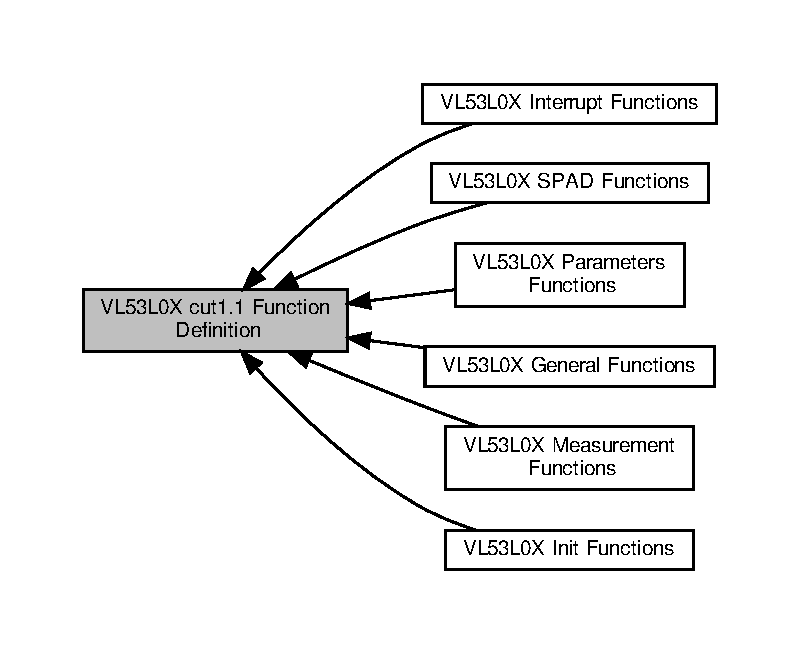
\includegraphics[width=350pt]{group__VL53L0X__cut11__group}
\end{center}
\end{figure}
\subsection*{Modules}
\begin{DoxyCompactItemize}
\item 
\hyperlink{group__VL53L0X__general__group}{V\+L53\+L0\+X General Functions}
\begin{DoxyCompactList}\small\item\em General functions and definitions. \end{DoxyCompactList}\item 
\hyperlink{group__VL53L0X__init__group}{V\+L53\+L0\+X Init Functions}
\begin{DoxyCompactList}\small\item\em V\+L53\+L0X Init Functions. \end{DoxyCompactList}\item 
\hyperlink{group__VL53L0X__parameters__group}{V\+L53\+L0\+X Parameters Functions}
\begin{DoxyCompactList}\small\item\em Functions used to prepare and setup the device. \end{DoxyCompactList}\item 
\hyperlink{group__VL53L0X__measurement__group}{V\+L53\+L0\+X Measurement Functions}
\begin{DoxyCompactList}\small\item\em Functions used for the measurements. \end{DoxyCompactList}\item 
\hyperlink{group__VL53L0X__interrupt__group}{V\+L53\+L0\+X Interrupt Functions}
\begin{DoxyCompactList}\small\item\em Functions used for interrupt managements. \end{DoxyCompactList}\item 
\hyperlink{group__VL53L0X__SPADfunctions__group}{V\+L53\+L0\+X S\+P\+A\+D Functions}
\begin{DoxyCompactList}\small\item\em Functions used for S\+P\+AD managements. \end{DoxyCompactList}\end{DoxyCompactItemize}


\subsection{Detailed Description}
V\+L53\+L0X cut1.\+1 Function Definition. 


\hypertarget{group__VL53L0X__general__group}{}\section{V\+L53\+L0X General Functions}
\label{group__VL53L0X__general__group}\index{V\+L53\+L0\+X General Functions@{V\+L53\+L0\+X General Functions}}


General functions and definitions.  


Collaboration diagram for V\+L53\+L0X General Functions\+:\nopagebreak
\begin{figure}[H]
\begin{center}
\leavevmode
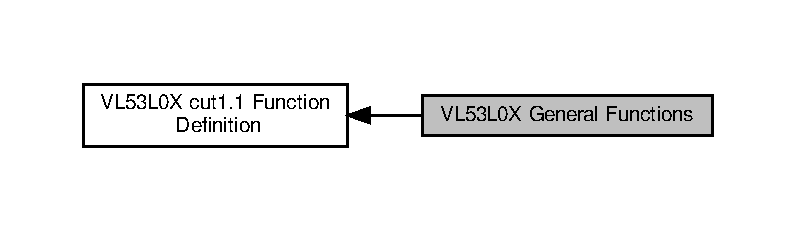
\includegraphics[width=350pt]{group__VL53L0X__general__group}
\end{center}
\end{figure}
\subsection*{Functions}
\begin{DoxyCompactItemize}
\item 
V\+L53\+L0\+X\+\_\+\+A\+PI V\+L53\+L0\+X\+\_\+\+Error \hyperlink{group__VL53L0X__general__group_gadb15b4f97b7218b3bdf571f90c27ec5e}{V\+L53\+L0\+X\+\_\+\+Get\+Version} (\hyperlink{structVL53L0X__Version__t}{V\+L53\+L0\+X\+\_\+\+Version\+\_\+t} $\ast$p\+Version)
\begin{DoxyCompactList}\small\item\em Return the V\+L53\+L0X P\+AL Implementation Version. \end{DoxyCompactList}\item 
V\+L53\+L0\+X\+\_\+\+A\+PI V\+L53\+L0\+X\+\_\+\+Error \hyperlink{group__VL53L0X__general__group_gad66c4309fbbf14d68692c18982158fba}{V\+L53\+L0\+X\+\_\+\+Get\+Pal\+Spec\+Version} (\hyperlink{structVL53L0X__Version__t}{V\+L53\+L0\+X\+\_\+\+Version\+\_\+t} $\ast$p\+Pal\+Spec\+Version)
\begin{DoxyCompactList}\small\item\em Return the P\+AL Specification Version used for the current implementation. \end{DoxyCompactList}\item 
V\+L53\+L0\+X\+\_\+\+A\+PI V\+L53\+L0\+X\+\_\+\+Error \hyperlink{group__VL53L0X__general__group_ga61bbb7db521494b59d82f0c0ee359260}{V\+L53\+L0\+X\+\_\+\+Get\+Product\+Revision} (\hyperlink{group__VL53L0X__platform__group_ga2d6405308b1dd524b462f1b8fb97d167}{V\+L53\+L0\+X\+\_\+\+D\+EV} Dev, \hyperlink{vl53l0x__types_8h_aba7bc1797add20fe3efdf37ced1182c5}{uint8\+\_\+t} $\ast$p\+Product\+Revision\+Major, \hyperlink{vl53l0x__types_8h_aba7bc1797add20fe3efdf37ced1182c5}{uint8\+\_\+t} $\ast$p\+Product\+Revision\+Minor)
\begin{DoxyCompactList}\small\item\em Reads the Product Revision for a for given Device This function can be used to distinguish cut1.\+0 from cut1.\+1. \end{DoxyCompactList}\item 
V\+L53\+L0\+X\+\_\+\+A\+PI V\+L53\+L0\+X\+\_\+\+Error \hyperlink{group__VL53L0X__general__group_ga608dd0345885215992789821cb094e17}{V\+L53\+L0\+X\+\_\+\+Get\+Device\+Info} (\hyperlink{group__VL53L0X__platform__group_ga2d6405308b1dd524b462f1b8fb97d167}{V\+L53\+L0\+X\+\_\+\+D\+EV} Dev, \hyperlink{structVL53L0X__DeviceInfo__t}{V\+L53\+L0\+X\+\_\+\+Device\+Info\+\_\+t} $\ast$p\+V\+L53\+L0\+X\+\_\+\+Device\+Info)
\begin{DoxyCompactList}\small\item\em Reads the Device information for given Device. \end{DoxyCompactList}\item 
V\+L53\+L0\+X\+\_\+\+A\+PI V\+L53\+L0\+X\+\_\+\+Error \hyperlink{group__VL53L0X__general__group_gad8bd4b6c24974fd55102615aed0efa14}{V\+L53\+L0\+X\+\_\+\+Get\+Device\+Error\+Status} (\hyperlink{group__VL53L0X__platform__group_ga2d6405308b1dd524b462f1b8fb97d167}{V\+L53\+L0\+X\+\_\+\+D\+EV} Dev, V\+L53\+L0\+X\+\_\+\+Device\+Error $\ast$p\+Device\+Error\+Status)
\begin{DoxyCompactList}\small\item\em Read current status of the error register for the selected device. \end{DoxyCompactList}\item 
V\+L53\+L0\+X\+\_\+\+A\+PI V\+L53\+L0\+X\+\_\+\+Error \hyperlink{group__VL53L0X__general__group_gad9a6d74d1c0b18a2180b896dc144ad7c}{V\+L53\+L0\+X\+\_\+\+Get\+Range\+Status\+String} (\hyperlink{vl53l0x__types_8h_aba7bc1797add20fe3efdf37ced1182c5}{uint8\+\_\+t} Range\+Status, char $\ast$p\+Range\+Status\+String)
\begin{DoxyCompactList}\small\item\em Human readable Range Status string for a given Range\+Status. \end{DoxyCompactList}\item 
V\+L53\+L0\+X\+\_\+\+A\+PI V\+L53\+L0\+X\+\_\+\+Error \hyperlink{group__VL53L0X__general__group_ga3532722a77431334a391fb8247cd334f}{V\+L53\+L0\+X\+\_\+\+Get\+Device\+Error\+String} (V\+L53\+L0\+X\+\_\+\+Device\+Error Error\+Code, char $\ast$p\+Device\+Error\+String)
\begin{DoxyCompactList}\small\item\em Human readable error string for a given Error Code. \end{DoxyCompactList}\item 
V\+L53\+L0\+X\+\_\+\+A\+PI V\+L53\+L0\+X\+\_\+\+Error \hyperlink{group__VL53L0X__general__group_gaa647e7ed8b78178968fab9b3562ebac7}{V\+L53\+L0\+X\+\_\+\+Get\+Pal\+Error\+String} (V\+L53\+L0\+X\+\_\+\+Error Pal\+Error\+Code, char $\ast$p\+Pal\+Error\+String)
\begin{DoxyCompactList}\small\item\em Human readable error string for current P\+AL error status. \end{DoxyCompactList}\item 
V\+L53\+L0\+X\+\_\+\+A\+PI V\+L53\+L0\+X\+\_\+\+Error \hyperlink{group__VL53L0X__general__group_ga1897c54c56a85fab54012ea53a444b23}{V\+L53\+L0\+X\+\_\+\+Get\+Pal\+State\+String} (V\+L53\+L0\+X\+\_\+\+State Pal\+State\+Code, char $\ast$p\+Pal\+State\+String)
\begin{DoxyCompactList}\small\item\em Human readable P\+AL State string. \end{DoxyCompactList}\item 
V\+L53\+L0\+X\+\_\+\+A\+PI V\+L53\+L0\+X\+\_\+\+Error \hyperlink{group__VL53L0X__general__group_gac4b91d3adc134655064fcc2c4a9adf24}{V\+L53\+L0\+X\+\_\+\+Get\+Pal\+State} (\hyperlink{group__VL53L0X__platform__group_ga2d6405308b1dd524b462f1b8fb97d167}{V\+L53\+L0\+X\+\_\+\+D\+EV} Dev, V\+L53\+L0\+X\+\_\+\+State $\ast$p\+Pal\+State)
\begin{DoxyCompactList}\small\item\em Reads the internal state of the P\+AL for a given Device. \end{DoxyCompactList}\item 
V\+L53\+L0\+X\+\_\+\+A\+PI V\+L53\+L0\+X\+\_\+\+Error \hyperlink{group__VL53L0X__general__group_ga8b435ab0813267fca1546c7da732c1f2}{V\+L53\+L0\+X\+\_\+\+Set\+Power\+Mode} (\hyperlink{group__VL53L0X__platform__group_ga2d6405308b1dd524b462f1b8fb97d167}{V\+L53\+L0\+X\+\_\+\+D\+EV} Dev, V\+L53\+L0\+X\+\_\+\+Power\+Modes Power\+Mode)
\begin{DoxyCompactList}\small\item\em Set the power mode for a given Device \hyperlink{structThe}{The} power mode can be Standby or Idle. Different level of both Standby and Idle can exists. This function should not be used when device is in Ranging state. \end{DoxyCompactList}\item 
V\+L53\+L0\+X\+\_\+\+A\+PI V\+L53\+L0\+X\+\_\+\+Error \hyperlink{group__VL53L0X__general__group_ga53faed55c6951878c58b6a19d613ee9b}{V\+L53\+L0\+X\+\_\+\+Get\+Power\+Mode} (\hyperlink{group__VL53L0X__platform__group_ga2d6405308b1dd524b462f1b8fb97d167}{V\+L53\+L0\+X\+\_\+\+D\+EV} Dev, V\+L53\+L0\+X\+\_\+\+Power\+Modes $\ast$p\+Power\+Mode)
\begin{DoxyCompactList}\small\item\em Get the power mode for a given Device. \end{DoxyCompactList}\item 
V\+L53\+L0\+X\+\_\+\+A\+PI V\+L53\+L0\+X\+\_\+\+Error \hyperlink{group__VL53L0X__general__group_ga6d87e7c39e30ede9f158362624487718}{V\+L53\+L0\+X\+\_\+\+Set\+Offset\+Calibration\+Data\+Micro\+Meter} (\hyperlink{group__VL53L0X__platform__group_ga2d6405308b1dd524b462f1b8fb97d167}{V\+L53\+L0\+X\+\_\+\+D\+EV} Dev, \hyperlink{vl53l0x__types_8h_a32f2e37ee053cf2ce8ca28d1f74630e5}{int32\+\_\+t} Offset\+Calibration\+Data\+Micro\+Meter)
\item 
V\+L53\+L0\+X\+\_\+\+A\+PI V\+L53\+L0\+X\+\_\+\+Error \hyperlink{group__VL53L0X__general__group_ga724ec9400a6d5667e10bda476cc43029}{V\+L53\+L0\+X\+\_\+\+Get\+Offset\+Calibration\+Data\+Micro\+Meter} (\hyperlink{group__VL53L0X__platform__group_ga2d6405308b1dd524b462f1b8fb97d167}{V\+L53\+L0\+X\+\_\+\+D\+EV} Dev, \hyperlink{vl53l0x__types_8h_a32f2e37ee053cf2ce8ca28d1f74630e5}{int32\+\_\+t} $\ast$p\+Offset\+Calibration\+Data\+Micro\+Meter)
\begin{DoxyCompactList}\small\item\em Get part to part calibration offset. \end{DoxyCompactList}\item 
V\+L53\+L0\+X\+\_\+\+A\+PI V\+L53\+L0\+X\+\_\+\+Error \hyperlink{group__VL53L0X__general__group_ga9dca9bb612d109f31caae8f1eef38ac7}{V\+L53\+L0\+X\+\_\+\+Set\+Linearity\+Corrective\+Gain} (\hyperlink{group__VL53L0X__platform__group_ga2d6405308b1dd524b462f1b8fb97d167}{V\+L53\+L0\+X\+\_\+\+D\+EV} Dev, \hyperlink{vl53l0x__types_8h_aa343fa3b3d06292b959ffdd4c4703b06}{int16\+\_\+t} Linearity\+Corrective\+Gain)
\item 
V\+L53\+L0\+X\+\_\+\+A\+PI V\+L53\+L0\+X\+\_\+\+Error \hyperlink{group__VL53L0X__general__group_ga921717fe0182527ce358b9c5ded340f1}{V\+L53\+L0\+X\+\_\+\+Get\+Linearity\+Corrective\+Gain} (\hyperlink{group__VL53L0X__platform__group_ga2d6405308b1dd524b462f1b8fb97d167}{V\+L53\+L0\+X\+\_\+\+D\+EV} Dev, \hyperlink{vl53l0x__types_8h_a273cf69d639a59973b6019625df33e30}{uint16\+\_\+t} $\ast$p\+Linearity\+Corrective\+Gain)
\begin{DoxyCompactList}\small\item\em Get the linearity corrective gain. \end{DoxyCompactList}\item 
V\+L53\+L0\+X\+\_\+\+A\+PI V\+L53\+L0\+X\+\_\+\+Error \hyperlink{group__VL53L0X__general__group_ga907d0e788b6ea0c7368a4c5133e0cb6a}{V\+L53\+L0\+X\+\_\+\+Set\+Group\+Param\+Hold} (\hyperlink{group__VL53L0X__platform__group_ga2d6405308b1dd524b462f1b8fb97d167}{V\+L53\+L0\+X\+\_\+\+D\+EV} Dev, \hyperlink{vl53l0x__types_8h_aba7bc1797add20fe3efdf37ced1182c5}{uint8\+\_\+t} Group\+Param\+Hold)
\item 
V\+L53\+L0\+X\+\_\+\+A\+PI V\+L53\+L0\+X\+\_\+\+Error \hyperlink{group__VL53L0X__general__group_gafa2d49e10b749cd6e57e50823184fea7}{V\+L53\+L0\+X\+\_\+\+Get\+Upper\+Limit\+Milli\+Meter} (\hyperlink{group__VL53L0X__platform__group_ga2d6405308b1dd524b462f1b8fb97d167}{V\+L53\+L0\+X\+\_\+\+D\+EV} Dev, \hyperlink{vl53l0x__types_8h_a273cf69d639a59973b6019625df33e30}{uint16\+\_\+t} $\ast$p\+Upper\+Limit\+Milli\+Meter)
\begin{DoxyCompactList}\small\item\em Get the maximal distance for actual setup. \end{DoxyCompactList}\item 
V\+L53\+L0\+X\+\_\+\+Error \hyperlink{group__VL53L0X__general__group_gaee98657af1e74394c5e3fc4d4b383dbf}{V\+L53\+L0\+X\+\_\+\+Get\+Total\+Signal\+Rate} (\hyperlink{group__VL53L0X__platform__group_ga2d6405308b1dd524b462f1b8fb97d167}{V\+L53\+L0\+X\+\_\+\+D\+EV} Dev, \hyperlink{vl53l0x__types_8h_afb910790161809fc76e1a274a6349384}{Fix\+Point1616\+\_\+t} $\ast$p\+Total\+Signal\+Rate)
\begin{DoxyCompactList}\small\item\em Get the Total Signal Rate. \end{DoxyCompactList}\end{DoxyCompactItemize}


\subsection{Detailed Description}
General functions and definitions. 



\subsection{Function Documentation}
\mbox{\Hypertarget{group__VL53L0X__general__group_gad8bd4b6c24974fd55102615aed0efa14}\label{group__VL53L0X__general__group_gad8bd4b6c24974fd55102615aed0efa14}} 
\index{V\+L53\+L0\+X General Functions@{V\+L53\+L0\+X General Functions}!V\+L53\+L0\+X\+\_\+\+Get\+Device\+Error\+Status@{V\+L53\+L0\+X\+\_\+\+Get\+Device\+Error\+Status}}
\index{V\+L53\+L0\+X\+\_\+\+Get\+Device\+Error\+Status@{V\+L53\+L0\+X\+\_\+\+Get\+Device\+Error\+Status}!V\+L53\+L0\+X General Functions@{V\+L53\+L0\+X General Functions}}
\subsubsection{\texorpdfstring{V\+L53\+L0\+X\+\_\+\+Get\+Device\+Error\+Status()}{VL53L0X\_GetDeviceErrorStatus()}}
{\footnotesize\ttfamily V\+L53\+L0\+X\+\_\+\+A\+PI V\+L53\+L0\+X\+\_\+\+Error V\+L53\+L0\+X\+\_\+\+Get\+Device\+Error\+Status (\begin{DoxyParamCaption}\item[{\hyperlink{group__VL53L0X__platform__group_ga2d6405308b1dd524b462f1b8fb97d167}{V\+L53\+L0\+X\+\_\+\+D\+EV}}]{Dev,  }\item[{V\+L53\+L0\+X\+\_\+\+Device\+Error $\ast$}]{p\+Device\+Error\+Status }\end{DoxyParamCaption})}



Read current status of the error register for the selected device. 

\begin{DoxyNote}{Note}
This function Access to the device
\end{DoxyNote}

\begin{DoxyParams}{Parameters}
{\em Dev} & Device Handle \\
\hline
{\em p\+Device\+Error\+Status} & Pointer to current error code of the device \\
\hline
\end{DoxyParams}
\begin{DoxyReturn}{Returns}
V\+L53\+L0\+X\+\_\+\+E\+R\+R\+O\+R\+\_\+\+N\+O\+NE Success 

\char`\"{}\+Other error code\char`\"{} See \+::\+V\+L53\+L0\+X\+\_\+\+Error 
\end{DoxyReturn}
\mbox{\Hypertarget{group__VL53L0X__general__group_ga3532722a77431334a391fb8247cd334f}\label{group__VL53L0X__general__group_ga3532722a77431334a391fb8247cd334f}} 
\index{V\+L53\+L0\+X General Functions@{V\+L53\+L0\+X General Functions}!V\+L53\+L0\+X\+\_\+\+Get\+Device\+Error\+String@{V\+L53\+L0\+X\+\_\+\+Get\+Device\+Error\+String}}
\index{V\+L53\+L0\+X\+\_\+\+Get\+Device\+Error\+String@{V\+L53\+L0\+X\+\_\+\+Get\+Device\+Error\+String}!V\+L53\+L0\+X General Functions@{V\+L53\+L0\+X General Functions}}
\subsubsection{\texorpdfstring{V\+L53\+L0\+X\+\_\+\+Get\+Device\+Error\+String()}{VL53L0X\_GetDeviceErrorString()}}
{\footnotesize\ttfamily V\+L53\+L0\+X\+\_\+\+A\+PI V\+L53\+L0\+X\+\_\+\+Error V\+L53\+L0\+X\+\_\+\+Get\+Device\+Error\+String (\begin{DoxyParamCaption}\item[{V\+L53\+L0\+X\+\_\+\+Device\+Error}]{Error\+Code,  }\item[{char $\ast$}]{p\+Device\+Error\+String }\end{DoxyParamCaption})}



Human readable error string for a given Error Code. 

\begin{DoxyNote}{Note}
This function doesn\textquotesingle{}t access to the device
\end{DoxyNote}

\begin{DoxyParams}{Parameters}
{\em Error\+Code} & \hyperlink{structThe}{The} error code as stored on \+::\+V\+L53\+L0\+X\+\_\+\+Device\+Error \\
\hline
{\em p\+Device\+Error\+String} & \hyperlink{structThe}{The} error string corresponding to the Error\+Code \\
\hline
\end{DoxyParams}
\begin{DoxyReturn}{Returns}
V\+L53\+L0\+X\+\_\+\+E\+R\+R\+O\+R\+\_\+\+N\+O\+NE Success 

\char`\"{}\+Other error code\char`\"{} See \+::\+V\+L53\+L0\+X\+\_\+\+Error 
\end{DoxyReturn}
\mbox{\Hypertarget{group__VL53L0X__general__group_ga608dd0345885215992789821cb094e17}\label{group__VL53L0X__general__group_ga608dd0345885215992789821cb094e17}} 
\index{V\+L53\+L0\+X General Functions@{V\+L53\+L0\+X General Functions}!V\+L53\+L0\+X\+\_\+\+Get\+Device\+Info@{V\+L53\+L0\+X\+\_\+\+Get\+Device\+Info}}
\index{V\+L53\+L0\+X\+\_\+\+Get\+Device\+Info@{V\+L53\+L0\+X\+\_\+\+Get\+Device\+Info}!V\+L53\+L0\+X General Functions@{V\+L53\+L0\+X General Functions}}
\subsubsection{\texorpdfstring{V\+L53\+L0\+X\+\_\+\+Get\+Device\+Info()}{VL53L0X\_GetDeviceInfo()}}
{\footnotesize\ttfamily V\+L53\+L0\+X\+\_\+\+A\+PI V\+L53\+L0\+X\+\_\+\+Error V\+L53\+L0\+X\+\_\+\+Get\+Device\+Info (\begin{DoxyParamCaption}\item[{\hyperlink{group__VL53L0X__platform__group_ga2d6405308b1dd524b462f1b8fb97d167}{V\+L53\+L0\+X\+\_\+\+D\+EV}}]{Dev,  }\item[{\hyperlink{structVL53L0X__DeviceInfo__t}{V\+L53\+L0\+X\+\_\+\+Device\+Info\+\_\+t} $\ast$}]{p\+V\+L53\+L0\+X\+\_\+\+Device\+Info }\end{DoxyParamCaption})}



Reads the Device information for given Device. 

\begin{DoxyNote}{Note}
This function Access to the device
\end{DoxyNote}

\begin{DoxyParams}{Parameters}
{\em Dev} & Device Handle \\
\hline
{\em p\+V\+L53\+L0\+X\+\_\+\+Device\+Info} & Pointer to current device info for a given Device \\
\hline
\end{DoxyParams}
\begin{DoxyReturn}{Returns}
V\+L53\+L0\+X\+\_\+\+E\+R\+R\+O\+R\+\_\+\+N\+O\+NE Success 

\char`\"{}\+Other error code\char`\"{} See \+::\+V\+L53\+L0\+X\+\_\+\+Error 
\end{DoxyReturn}
\mbox{\Hypertarget{group__VL53L0X__general__group_ga921717fe0182527ce358b9c5ded340f1}\label{group__VL53L0X__general__group_ga921717fe0182527ce358b9c5ded340f1}} 
\index{V\+L53\+L0\+X General Functions@{V\+L53\+L0\+X General Functions}!V\+L53\+L0\+X\+\_\+\+Get\+Linearity\+Corrective\+Gain@{V\+L53\+L0\+X\+\_\+\+Get\+Linearity\+Corrective\+Gain}}
\index{V\+L53\+L0\+X\+\_\+\+Get\+Linearity\+Corrective\+Gain@{V\+L53\+L0\+X\+\_\+\+Get\+Linearity\+Corrective\+Gain}!V\+L53\+L0\+X General Functions@{V\+L53\+L0\+X General Functions}}
\subsubsection{\texorpdfstring{V\+L53\+L0\+X\+\_\+\+Get\+Linearity\+Corrective\+Gain()}{VL53L0X\_GetLinearityCorrectiveGain()}}
{\footnotesize\ttfamily V\+L53\+L0\+X\+\_\+\+A\+PI V\+L53\+L0\+X\+\_\+\+Error V\+L53\+L0\+X\+\_\+\+Get\+Linearity\+Corrective\+Gain (\begin{DoxyParamCaption}\item[{\hyperlink{group__VL53L0X__platform__group_ga2d6405308b1dd524b462f1b8fb97d167}{V\+L53\+L0\+X\+\_\+\+D\+EV}}]{Dev,  }\item[{\hyperlink{vl53l0x__types_8h_a273cf69d639a59973b6019625df33e30}{uint16\+\_\+t} $\ast$}]{p\+Linearity\+Corrective\+Gain }\end{DoxyParamCaption})}



Get the linearity corrective gain. 

\begin{DoxyParagraph}{Function Description}
Should only be used after a successful call to {\itshape V\+L53\+L0\+X\+\_\+\+Data\+Init} to backup device N\+VM value
\end{DoxyParagraph}
\begin{DoxyNote}{Note}
This function Access to the device
\end{DoxyNote}

\begin{DoxyParams}{Parameters}
{\em Dev} & Device Handle \\
\hline
{\em p\+Linearity\+Corrective\+Gain} & Pointer to the linearity corrective gain in x1000 if value is 1000 then no modification is applied. \\
\hline
\end{DoxyParams}
\begin{DoxyReturn}{Returns}
V\+L53\+L0\+X\+\_\+\+E\+R\+R\+O\+R\+\_\+\+N\+O\+NE Success 

\char`\"{}\+Other error code\char`\"{} See \+::\+V\+L53\+L0\+X\+\_\+\+Error 
\end{DoxyReturn}
\mbox{\Hypertarget{group__VL53L0X__general__group_ga724ec9400a6d5667e10bda476cc43029}\label{group__VL53L0X__general__group_ga724ec9400a6d5667e10bda476cc43029}} 
\index{V\+L53\+L0\+X General Functions@{V\+L53\+L0\+X General Functions}!V\+L53\+L0\+X\+\_\+\+Get\+Offset\+Calibration\+Data\+Micro\+Meter@{V\+L53\+L0\+X\+\_\+\+Get\+Offset\+Calibration\+Data\+Micro\+Meter}}
\index{V\+L53\+L0\+X\+\_\+\+Get\+Offset\+Calibration\+Data\+Micro\+Meter@{V\+L53\+L0\+X\+\_\+\+Get\+Offset\+Calibration\+Data\+Micro\+Meter}!V\+L53\+L0\+X General Functions@{V\+L53\+L0\+X General Functions}}
\subsubsection{\texorpdfstring{V\+L53\+L0\+X\+\_\+\+Get\+Offset\+Calibration\+Data\+Micro\+Meter()}{VL53L0X\_GetOffsetCalibrationDataMicroMeter()}}
{\footnotesize\ttfamily V\+L53\+L0\+X\+\_\+\+A\+PI V\+L53\+L0\+X\+\_\+\+Error V\+L53\+L0\+X\+\_\+\+Get\+Offset\+Calibration\+Data\+Micro\+Meter (\begin{DoxyParamCaption}\item[{\hyperlink{group__VL53L0X__platform__group_ga2d6405308b1dd524b462f1b8fb97d167}{V\+L53\+L0\+X\+\_\+\+D\+EV}}]{Dev,  }\item[{\hyperlink{vl53l0x__types_8h_a32f2e37ee053cf2ce8ca28d1f74630e5}{int32\+\_\+t} $\ast$}]{p\+Offset\+Calibration\+Data\+Micro\+Meter }\end{DoxyParamCaption})}



Get part to part calibration offset. 

\begin{DoxyParagraph}{Function Description}
Should only be used after a successful call to {\itshape V\+L53\+L0\+X\+\_\+\+Data\+Init} to backup device N\+VM value
\end{DoxyParagraph}
\begin{DoxyNote}{Note}
This function Access to the device
\end{DoxyNote}

\begin{DoxyParams}{Parameters}
{\em Dev} & Device Handle \\
\hline
{\em p\+Offset\+Calibration\+Data\+Micro\+Meter} & Return part to part calibration offset from device (microns) \\
\hline
\end{DoxyParams}
\begin{DoxyReturn}{Returns}
V\+L53\+L0\+X\+\_\+\+E\+R\+R\+O\+R\+\_\+\+N\+O\+NE Success 

\char`\"{}\+Other error code\char`\"{} See \+::\+V\+L53\+L0\+X\+\_\+\+Error 
\end{DoxyReturn}
\mbox{\Hypertarget{group__VL53L0X__general__group_gaa647e7ed8b78178968fab9b3562ebac7}\label{group__VL53L0X__general__group_gaa647e7ed8b78178968fab9b3562ebac7}} 
\index{V\+L53\+L0\+X General Functions@{V\+L53\+L0\+X General Functions}!V\+L53\+L0\+X\+\_\+\+Get\+Pal\+Error\+String@{V\+L53\+L0\+X\+\_\+\+Get\+Pal\+Error\+String}}
\index{V\+L53\+L0\+X\+\_\+\+Get\+Pal\+Error\+String@{V\+L53\+L0\+X\+\_\+\+Get\+Pal\+Error\+String}!V\+L53\+L0\+X General Functions@{V\+L53\+L0\+X General Functions}}
\subsubsection{\texorpdfstring{V\+L53\+L0\+X\+\_\+\+Get\+Pal\+Error\+String()}{VL53L0X\_GetPalErrorString()}}
{\footnotesize\ttfamily V\+L53\+L0\+X\+\_\+\+A\+PI V\+L53\+L0\+X\+\_\+\+Error V\+L53\+L0\+X\+\_\+\+Get\+Pal\+Error\+String (\begin{DoxyParamCaption}\item[{V\+L53\+L0\+X\+\_\+\+Error}]{Pal\+Error\+Code,  }\item[{char $\ast$}]{p\+Pal\+Error\+String }\end{DoxyParamCaption})}



Human readable error string for current P\+AL error status. 

\begin{DoxyNote}{Note}
This function doesn\textquotesingle{}t access to the device
\end{DoxyNote}

\begin{DoxyParams}{Parameters}
{\em Pal\+Error\+Code} & \hyperlink{structThe}{The} error code as stored on {\itshape V\+L53\+L0\+X\+\_\+\+Error} \\
\hline
{\em p\+Pal\+Error\+String} & \hyperlink{structThe}{The} error string corresponding to the Pal\+Error\+Code \\
\hline
\end{DoxyParams}
\begin{DoxyReturn}{Returns}
V\+L53\+L0\+X\+\_\+\+E\+R\+R\+O\+R\+\_\+\+N\+O\+NE Success 

\char`\"{}\+Other error code\char`\"{} See \+::\+V\+L53\+L0\+X\+\_\+\+Error 
\end{DoxyReturn}
\mbox{\Hypertarget{group__VL53L0X__general__group_gad66c4309fbbf14d68692c18982158fba}\label{group__VL53L0X__general__group_gad66c4309fbbf14d68692c18982158fba}} 
\index{V\+L53\+L0\+X General Functions@{V\+L53\+L0\+X General Functions}!V\+L53\+L0\+X\+\_\+\+Get\+Pal\+Spec\+Version@{V\+L53\+L0\+X\+\_\+\+Get\+Pal\+Spec\+Version}}
\index{V\+L53\+L0\+X\+\_\+\+Get\+Pal\+Spec\+Version@{V\+L53\+L0\+X\+\_\+\+Get\+Pal\+Spec\+Version}!V\+L53\+L0\+X General Functions@{V\+L53\+L0\+X General Functions}}
\subsubsection{\texorpdfstring{V\+L53\+L0\+X\+\_\+\+Get\+Pal\+Spec\+Version()}{VL53L0X\_GetPalSpecVersion()}}
{\footnotesize\ttfamily V\+L53\+L0\+X\+\_\+\+A\+PI V\+L53\+L0\+X\+\_\+\+Error V\+L53\+L0\+X\+\_\+\+Get\+Pal\+Spec\+Version (\begin{DoxyParamCaption}\item[{\hyperlink{structVL53L0X__Version__t}{V\+L53\+L0\+X\+\_\+\+Version\+\_\+t} $\ast$}]{p\+Pal\+Spec\+Version }\end{DoxyParamCaption})}



Return the P\+AL Specification Version used for the current implementation. 

\begin{DoxyNote}{Note}
This function doesn\textquotesingle{}t access to the device
\end{DoxyNote}

\begin{DoxyParams}{Parameters}
{\em p\+Pal\+Spec\+Version} & Pointer to current P\+AL Specification Version \\
\hline
\end{DoxyParams}
\begin{DoxyReturn}{Returns}
V\+L53\+L0\+X\+\_\+\+E\+R\+R\+O\+R\+\_\+\+N\+O\+NE Success 

\char`\"{}\+Other error code\char`\"{} See \+::\+V\+L53\+L0\+X\+\_\+\+Error 
\end{DoxyReturn}
\mbox{\Hypertarget{group__VL53L0X__general__group_gac4b91d3adc134655064fcc2c4a9adf24}\label{group__VL53L0X__general__group_gac4b91d3adc134655064fcc2c4a9adf24}} 
\index{V\+L53\+L0\+X General Functions@{V\+L53\+L0\+X General Functions}!V\+L53\+L0\+X\+\_\+\+Get\+Pal\+State@{V\+L53\+L0\+X\+\_\+\+Get\+Pal\+State}}
\index{V\+L53\+L0\+X\+\_\+\+Get\+Pal\+State@{V\+L53\+L0\+X\+\_\+\+Get\+Pal\+State}!V\+L53\+L0\+X General Functions@{V\+L53\+L0\+X General Functions}}
\subsubsection{\texorpdfstring{V\+L53\+L0\+X\+\_\+\+Get\+Pal\+State()}{VL53L0X\_GetPalState()}}
{\footnotesize\ttfamily V\+L53\+L0\+X\+\_\+\+A\+PI V\+L53\+L0\+X\+\_\+\+Error V\+L53\+L0\+X\+\_\+\+Get\+Pal\+State (\begin{DoxyParamCaption}\item[{\hyperlink{group__VL53L0X__platform__group_ga2d6405308b1dd524b462f1b8fb97d167}{V\+L53\+L0\+X\+\_\+\+D\+EV}}]{Dev,  }\item[{V\+L53\+L0\+X\+\_\+\+State $\ast$}]{p\+Pal\+State }\end{DoxyParamCaption})}



Reads the internal state of the P\+AL for a given Device. 

\begin{DoxyNote}{Note}
This function doesn\textquotesingle{}t access to the device
\end{DoxyNote}

\begin{DoxyParams}{Parameters}
{\em Dev} & Device Handle \\
\hline
{\em p\+Pal\+State} & Pointer to current state of the P\+AL for a given Device \\
\hline
\end{DoxyParams}
\begin{DoxyReturn}{Returns}
V\+L53\+L0\+X\+\_\+\+E\+R\+R\+O\+R\+\_\+\+N\+O\+NE Success 

\char`\"{}\+Other error code\char`\"{} See \+::\+V\+L53\+L0\+X\+\_\+\+Error 
\end{DoxyReturn}
\mbox{\Hypertarget{group__VL53L0X__general__group_ga1897c54c56a85fab54012ea53a444b23}\label{group__VL53L0X__general__group_ga1897c54c56a85fab54012ea53a444b23}} 
\index{V\+L53\+L0\+X General Functions@{V\+L53\+L0\+X General Functions}!V\+L53\+L0\+X\+\_\+\+Get\+Pal\+State\+String@{V\+L53\+L0\+X\+\_\+\+Get\+Pal\+State\+String}}
\index{V\+L53\+L0\+X\+\_\+\+Get\+Pal\+State\+String@{V\+L53\+L0\+X\+\_\+\+Get\+Pal\+State\+String}!V\+L53\+L0\+X General Functions@{V\+L53\+L0\+X General Functions}}
\subsubsection{\texorpdfstring{V\+L53\+L0\+X\+\_\+\+Get\+Pal\+State\+String()}{VL53L0X\_GetPalStateString()}}
{\footnotesize\ttfamily V\+L53\+L0\+X\+\_\+\+A\+PI V\+L53\+L0\+X\+\_\+\+Error V\+L53\+L0\+X\+\_\+\+Get\+Pal\+State\+String (\begin{DoxyParamCaption}\item[{V\+L53\+L0\+X\+\_\+\+State}]{Pal\+State\+Code,  }\item[{char $\ast$}]{p\+Pal\+State\+String }\end{DoxyParamCaption})}



Human readable P\+AL State string. 

\begin{DoxyNote}{Note}
This function doesn\textquotesingle{}t access to the device
\end{DoxyNote}

\begin{DoxyParams}{Parameters}
{\em Pal\+State\+Code} & \hyperlink{structThe}{The} State code as stored on {\itshape V\+L53\+L0\+X\+\_\+\+State} \\
\hline
{\em p\+Pal\+State\+String} & \hyperlink{structThe}{The} State string corresponding to the Pal\+State\+Code \\
\hline
\end{DoxyParams}
\begin{DoxyReturn}{Returns}
V\+L53\+L0\+X\+\_\+\+E\+R\+R\+O\+R\+\_\+\+N\+O\+NE Success 

\char`\"{}\+Other error code\char`\"{} See \+::\+V\+L53\+L0\+X\+\_\+\+Error 
\end{DoxyReturn}
\mbox{\Hypertarget{group__VL53L0X__general__group_ga53faed55c6951878c58b6a19d613ee9b}\label{group__VL53L0X__general__group_ga53faed55c6951878c58b6a19d613ee9b}} 
\index{V\+L53\+L0\+X General Functions@{V\+L53\+L0\+X General Functions}!V\+L53\+L0\+X\+\_\+\+Get\+Power\+Mode@{V\+L53\+L0\+X\+\_\+\+Get\+Power\+Mode}}
\index{V\+L53\+L0\+X\+\_\+\+Get\+Power\+Mode@{V\+L53\+L0\+X\+\_\+\+Get\+Power\+Mode}!V\+L53\+L0\+X General Functions@{V\+L53\+L0\+X General Functions}}
\subsubsection{\texorpdfstring{V\+L53\+L0\+X\+\_\+\+Get\+Power\+Mode()}{VL53L0X\_GetPowerMode()}}
{\footnotesize\ttfamily V\+L53\+L0\+X\+\_\+\+A\+PI V\+L53\+L0\+X\+\_\+\+Error V\+L53\+L0\+X\+\_\+\+Get\+Power\+Mode (\begin{DoxyParamCaption}\item[{\hyperlink{group__VL53L0X__platform__group_ga2d6405308b1dd524b462f1b8fb97d167}{V\+L53\+L0\+X\+\_\+\+D\+EV}}]{Dev,  }\item[{V\+L53\+L0\+X\+\_\+\+Power\+Modes $\ast$}]{p\+Power\+Mode }\end{DoxyParamCaption})}



Get the power mode for a given Device. 

\begin{DoxyNote}{Note}
This function Access to the device
\end{DoxyNote}

\begin{DoxyParams}{Parameters}
{\em Dev} & Device Handle \\
\hline
{\em p\+Power\+Mode} & Pointer to the current value of the power mode. see \+::\+V\+L53\+L0\+X\+\_\+\+Power\+Modes Valid values are\+: V\+L53\+L0\+X\+\_\+\+P\+O\+W\+E\+R\+M\+O\+D\+E\+\_\+\+S\+T\+A\+N\+D\+B\+Y\+\_\+\+L\+E\+V\+E\+L1, V\+L53\+L0\+X\+\_\+\+P\+O\+W\+E\+R\+M\+O\+D\+E\+\_\+\+I\+D\+L\+E\+\_\+\+L\+E\+V\+E\+L1 \\
\hline
\end{DoxyParams}
\begin{DoxyReturn}{Returns}
V\+L53\+L0\+X\+\_\+\+E\+R\+R\+O\+R\+\_\+\+N\+O\+NE Success 

\char`\"{}\+Other error code\char`\"{} See \+::\+V\+L53\+L0\+X\+\_\+\+Error 
\end{DoxyReturn}
\mbox{\Hypertarget{group__VL53L0X__general__group_ga61bbb7db521494b59d82f0c0ee359260}\label{group__VL53L0X__general__group_ga61bbb7db521494b59d82f0c0ee359260}} 
\index{V\+L53\+L0\+X General Functions@{V\+L53\+L0\+X General Functions}!V\+L53\+L0\+X\+\_\+\+Get\+Product\+Revision@{V\+L53\+L0\+X\+\_\+\+Get\+Product\+Revision}}
\index{V\+L53\+L0\+X\+\_\+\+Get\+Product\+Revision@{V\+L53\+L0\+X\+\_\+\+Get\+Product\+Revision}!V\+L53\+L0\+X General Functions@{V\+L53\+L0\+X General Functions}}
\subsubsection{\texorpdfstring{V\+L53\+L0\+X\+\_\+\+Get\+Product\+Revision()}{VL53L0X\_GetProductRevision()}}
{\footnotesize\ttfamily V\+L53\+L0\+X\+\_\+\+A\+PI V\+L53\+L0\+X\+\_\+\+Error V\+L53\+L0\+X\+\_\+\+Get\+Product\+Revision (\begin{DoxyParamCaption}\item[{\hyperlink{group__VL53L0X__platform__group_ga2d6405308b1dd524b462f1b8fb97d167}{V\+L53\+L0\+X\+\_\+\+D\+EV}}]{Dev,  }\item[{\hyperlink{vl53l0x__types_8h_aba7bc1797add20fe3efdf37ced1182c5}{uint8\+\_\+t} $\ast$}]{p\+Product\+Revision\+Major,  }\item[{\hyperlink{vl53l0x__types_8h_aba7bc1797add20fe3efdf37ced1182c5}{uint8\+\_\+t} $\ast$}]{p\+Product\+Revision\+Minor }\end{DoxyParamCaption})}



Reads the Product Revision for a for given Device This function can be used to distinguish cut1.\+0 from cut1.\+1. 

\begin{DoxyNote}{Note}
This function Access to the device
\end{DoxyNote}

\begin{DoxyParams}{Parameters}
{\em Dev} & Device Handle \\
\hline
{\em p\+Product\+Revision\+Major} & Pointer to Product Revision Major for a given Device \\
\hline
{\em p\+Product\+Revision\+Minor} & Pointer to Product Revision Minor for a given Device \\
\hline
\end{DoxyParams}
\begin{DoxyReturn}{Returns}
V\+L53\+L0\+X\+\_\+\+E\+R\+R\+O\+R\+\_\+\+N\+O\+NE Success 

\char`\"{}\+Other error code\char`\"{} See \+::\+V\+L53\+L0\+X\+\_\+\+Error 
\end{DoxyReturn}
\mbox{\Hypertarget{group__VL53L0X__general__group_gad9a6d74d1c0b18a2180b896dc144ad7c}\label{group__VL53L0X__general__group_gad9a6d74d1c0b18a2180b896dc144ad7c}} 
\index{V\+L53\+L0\+X General Functions@{V\+L53\+L0\+X General Functions}!V\+L53\+L0\+X\+\_\+\+Get\+Range\+Status\+String@{V\+L53\+L0\+X\+\_\+\+Get\+Range\+Status\+String}}
\index{V\+L53\+L0\+X\+\_\+\+Get\+Range\+Status\+String@{V\+L53\+L0\+X\+\_\+\+Get\+Range\+Status\+String}!V\+L53\+L0\+X General Functions@{V\+L53\+L0\+X General Functions}}
\subsubsection{\texorpdfstring{V\+L53\+L0\+X\+\_\+\+Get\+Range\+Status\+String()}{VL53L0X\_GetRangeStatusString()}}
{\footnotesize\ttfamily V\+L53\+L0\+X\+\_\+\+A\+PI V\+L53\+L0\+X\+\_\+\+Error V\+L53\+L0\+X\+\_\+\+Get\+Range\+Status\+String (\begin{DoxyParamCaption}\item[{\hyperlink{vl53l0x__types_8h_aba7bc1797add20fe3efdf37ced1182c5}{uint8\+\_\+t}}]{Range\+Status,  }\item[{char $\ast$}]{p\+Range\+Status\+String }\end{DoxyParamCaption})}



Human readable Range Status string for a given Range\+Status. 

\begin{DoxyNote}{Note}
This function doesn\textquotesingle{}t access to the device
\end{DoxyNote}

\begin{DoxyParams}{Parameters}
{\em Range\+Status} & \hyperlink{structThe}{The} Range\+Status code as stored on {\itshape \hyperlink{structVL53L0X__RangingMeasurementData__t}{V\+L53\+L0\+X\+\_\+\+Ranging\+Measurement\+Data\+\_\+t}} \\
\hline
{\em p\+Range\+Status\+String} & \hyperlink{structThe}{The} returned Range\+Status string. \\
\hline
\end{DoxyParams}
\begin{DoxyReturn}{Returns}
V\+L53\+L0\+X\+\_\+\+E\+R\+R\+O\+R\+\_\+\+N\+O\+NE Success 

\char`\"{}\+Other error code\char`\"{} See \+::\+V\+L53\+L0\+X\+\_\+\+Error 
\end{DoxyReturn}
\mbox{\Hypertarget{group__VL53L0X__general__group_gaee98657af1e74394c5e3fc4d4b383dbf}\label{group__VL53L0X__general__group_gaee98657af1e74394c5e3fc4d4b383dbf}} 
\index{V\+L53\+L0\+X General Functions@{V\+L53\+L0\+X General Functions}!V\+L53\+L0\+X\+\_\+\+Get\+Total\+Signal\+Rate@{V\+L53\+L0\+X\+\_\+\+Get\+Total\+Signal\+Rate}}
\index{V\+L53\+L0\+X\+\_\+\+Get\+Total\+Signal\+Rate@{V\+L53\+L0\+X\+\_\+\+Get\+Total\+Signal\+Rate}!V\+L53\+L0\+X General Functions@{V\+L53\+L0\+X General Functions}}
\subsubsection{\texorpdfstring{V\+L53\+L0\+X\+\_\+\+Get\+Total\+Signal\+Rate()}{VL53L0X\_GetTotalSignalRate()}}
{\footnotesize\ttfamily V\+L53\+L0\+X\+\_\+\+Error V\+L53\+L0\+X\+\_\+\+Get\+Total\+Signal\+Rate (\begin{DoxyParamCaption}\item[{\hyperlink{group__VL53L0X__platform__group_ga2d6405308b1dd524b462f1b8fb97d167}{V\+L53\+L0\+X\+\_\+\+D\+EV}}]{Dev,  }\item[{\hyperlink{vl53l0x__types_8h_afb910790161809fc76e1a274a6349384}{Fix\+Point1616\+\_\+t} $\ast$}]{p\+Total\+Signal\+Rate }\end{DoxyParamCaption})}



Get the Total Signal Rate. 

\begin{DoxyParagraph}{Function Description}
This function will return the Total Signal Rate after a good ranging is done.
\end{DoxyParagraph}
\begin{DoxyNote}{Note}
This function access to Device
\end{DoxyNote}

\begin{DoxyParams}{Parameters}
{\em Dev} & Device Handle \\
\hline
{\em p\+Total\+Signal\+Rate} & Total Signal Rate value in Mega count per second \\
\hline
\end{DoxyParams}
\begin{DoxyReturn}{Returns}
V\+L53\+L0\+X\+\_\+\+E\+R\+R\+O\+R\+\_\+\+N\+O\+NE Success 

\char`\"{}\+Other error code\char`\"{} See \+::\+V\+L53\+L0\+X\+\_\+\+Error 
\end{DoxyReturn}
\mbox{\Hypertarget{group__VL53L0X__general__group_gafa2d49e10b749cd6e57e50823184fea7}\label{group__VL53L0X__general__group_gafa2d49e10b749cd6e57e50823184fea7}} 
\index{V\+L53\+L0\+X General Functions@{V\+L53\+L0\+X General Functions}!V\+L53\+L0\+X\+\_\+\+Get\+Upper\+Limit\+Milli\+Meter@{V\+L53\+L0\+X\+\_\+\+Get\+Upper\+Limit\+Milli\+Meter}}
\index{V\+L53\+L0\+X\+\_\+\+Get\+Upper\+Limit\+Milli\+Meter@{V\+L53\+L0\+X\+\_\+\+Get\+Upper\+Limit\+Milli\+Meter}!V\+L53\+L0\+X General Functions@{V\+L53\+L0\+X General Functions}}
\subsubsection{\texorpdfstring{V\+L53\+L0\+X\+\_\+\+Get\+Upper\+Limit\+Milli\+Meter()}{VL53L0X\_GetUpperLimitMilliMeter()}}
{\footnotesize\ttfamily V\+L53\+L0\+X\+\_\+\+A\+PI V\+L53\+L0\+X\+\_\+\+Error V\+L53\+L0\+X\+\_\+\+Get\+Upper\+Limit\+Milli\+Meter (\begin{DoxyParamCaption}\item[{\hyperlink{group__VL53L0X__platform__group_ga2d6405308b1dd524b462f1b8fb97d167}{V\+L53\+L0\+X\+\_\+\+D\+EV}}]{Dev,  }\item[{\hyperlink{vl53l0x__types_8h_a273cf69d639a59973b6019625df33e30}{uint16\+\_\+t} $\ast$}]{p\+Upper\+Limit\+Milli\+Meter }\end{DoxyParamCaption})}



Get the maximal distance for actual setup. 

\begin{DoxyParagraph}{Function Description}
Device must be initialized through {\itshape V\+L53\+L0\+X\+\_\+\+Set\+Parameters()} prior calling this function.
\end{DoxyParagraph}
Any range value more than the value returned is to be considered as \char`\"{}no target detected\char`\"{} or \char`\"{}no target in detectable range\char`\"{}~\newline
\begin{DoxyWarning}{Warning}
\hyperlink{structThe}{The} maximal distance depends on the setup
\end{DoxyWarning}
\begin{DoxyNote}{Note}
This function is not Implemented
\end{DoxyNote}

\begin{DoxyParams}{Parameters}
{\em Dev} & Device Handle \\
\hline
{\em p\+Upper\+Limit\+Milli\+Meter} & \hyperlink{structThe}{The} maximal range limit for actual setup (in millimeter) \\
\hline
\end{DoxyParams}
\begin{DoxyReturn}{Returns}
V\+L53\+L0\+X\+\_\+\+E\+R\+R\+O\+R\+\_\+\+N\+O\+T\+\_\+\+I\+M\+P\+L\+E\+M\+E\+N\+T\+ED Not implemented 
\end{DoxyReturn}
\mbox{\Hypertarget{group__VL53L0X__general__group_gadb15b4f97b7218b3bdf571f90c27ec5e}\label{group__VL53L0X__general__group_gadb15b4f97b7218b3bdf571f90c27ec5e}} 
\index{V\+L53\+L0\+X General Functions@{V\+L53\+L0\+X General Functions}!V\+L53\+L0\+X\+\_\+\+Get\+Version@{V\+L53\+L0\+X\+\_\+\+Get\+Version}}
\index{V\+L53\+L0\+X\+\_\+\+Get\+Version@{V\+L53\+L0\+X\+\_\+\+Get\+Version}!V\+L53\+L0\+X General Functions@{V\+L53\+L0\+X General Functions}}
\subsubsection{\texorpdfstring{V\+L53\+L0\+X\+\_\+\+Get\+Version()}{VL53L0X\_GetVersion()}}
{\footnotesize\ttfamily V\+L53\+L0\+X\+\_\+\+A\+PI V\+L53\+L0\+X\+\_\+\+Error V\+L53\+L0\+X\+\_\+\+Get\+Version (\begin{DoxyParamCaption}\item[{\hyperlink{structVL53L0X__Version__t}{V\+L53\+L0\+X\+\_\+\+Version\+\_\+t} $\ast$}]{p\+Version }\end{DoxyParamCaption})}



Return the V\+L53\+L0X P\+AL Implementation Version. 

\begin{DoxyNote}{Note}
This function doesn\textquotesingle{}t access to the device
\end{DoxyNote}

\begin{DoxyParams}{Parameters}
{\em p\+Version} & Pointer to current P\+AL Implementation Version \\
\hline
\end{DoxyParams}
\begin{DoxyReturn}{Returns}
V\+L53\+L0\+X\+\_\+\+E\+R\+R\+O\+R\+\_\+\+N\+O\+NE Success 

\char`\"{}\+Other error code\char`\"{} See \+::\+V\+L53\+L0\+X\+\_\+\+Error 
\end{DoxyReturn}
\mbox{\Hypertarget{group__VL53L0X__general__group_ga907d0e788b6ea0c7368a4c5133e0cb6a}\label{group__VL53L0X__general__group_ga907d0e788b6ea0c7368a4c5133e0cb6a}} 
\index{V\+L53\+L0\+X General Functions@{V\+L53\+L0\+X General Functions}!V\+L53\+L0\+X\+\_\+\+Set\+Group\+Param\+Hold@{V\+L53\+L0\+X\+\_\+\+Set\+Group\+Param\+Hold}}
\index{V\+L53\+L0\+X\+\_\+\+Set\+Group\+Param\+Hold@{V\+L53\+L0\+X\+\_\+\+Set\+Group\+Param\+Hold}!V\+L53\+L0\+X General Functions@{V\+L53\+L0\+X General Functions}}
\subsubsection{\texorpdfstring{V\+L53\+L0\+X\+\_\+\+Set\+Group\+Param\+Hold()}{VL53L0X\_SetGroupParamHold()}}
{\footnotesize\ttfamily V\+L53\+L0\+X\+\_\+\+A\+PI V\+L53\+L0\+X\+\_\+\+Error V\+L53\+L0\+X\+\_\+\+Set\+Group\+Param\+Hold (\begin{DoxyParamCaption}\item[{\hyperlink{group__VL53L0X__platform__group_ga2d6405308b1dd524b462f1b8fb97d167}{V\+L53\+L0\+X\+\_\+\+D\+EV}}]{Dev,  }\item[{\hyperlink{vl53l0x__types_8h_aba7bc1797add20fe3efdf37ced1182c5}{uint8\+\_\+t}}]{Group\+Param\+Hold }\end{DoxyParamCaption})}

Set Group parameter Hold state

\begin{DoxyParagraph}{Function Description}
Set or remove device internal group parameter hold
\end{DoxyParagraph}
\begin{DoxyNote}{Note}
This function is not Implemented
\end{DoxyNote}

\begin{DoxyParams}{Parameters}
{\em Dev} & Device Handle \\
\hline
{\em Group\+Param\+Hold} & Group parameter Hold state to be set (on/off) \\
\hline
\end{DoxyParams}
\begin{DoxyReturn}{Returns}
V\+L53\+L0\+X\+\_\+\+E\+R\+R\+O\+R\+\_\+\+N\+O\+T\+\_\+\+I\+M\+P\+L\+E\+M\+E\+N\+T\+ED Not implemented 
\end{DoxyReturn}
\mbox{\Hypertarget{group__VL53L0X__general__group_ga9dca9bb612d109f31caae8f1eef38ac7}\label{group__VL53L0X__general__group_ga9dca9bb612d109f31caae8f1eef38ac7}} 
\index{V\+L53\+L0\+X General Functions@{V\+L53\+L0\+X General Functions}!V\+L53\+L0\+X\+\_\+\+Set\+Linearity\+Corrective\+Gain@{V\+L53\+L0\+X\+\_\+\+Set\+Linearity\+Corrective\+Gain}}
\index{V\+L53\+L0\+X\+\_\+\+Set\+Linearity\+Corrective\+Gain@{V\+L53\+L0\+X\+\_\+\+Set\+Linearity\+Corrective\+Gain}!V\+L53\+L0\+X General Functions@{V\+L53\+L0\+X General Functions}}
\subsubsection{\texorpdfstring{V\+L53\+L0\+X\+\_\+\+Set\+Linearity\+Corrective\+Gain()}{VL53L0X\_SetLinearityCorrectiveGain()}}
{\footnotesize\ttfamily V\+L53\+L0\+X\+\_\+\+A\+PI V\+L53\+L0\+X\+\_\+\+Error V\+L53\+L0\+X\+\_\+\+Set\+Linearity\+Corrective\+Gain (\begin{DoxyParamCaption}\item[{\hyperlink{group__VL53L0X__platform__group_ga2d6405308b1dd524b462f1b8fb97d167}{V\+L53\+L0\+X\+\_\+\+D\+EV}}]{Dev,  }\item[{\hyperlink{vl53l0x__types_8h_aa343fa3b3d06292b959ffdd4c4703b06}{int16\+\_\+t}}]{Linearity\+Corrective\+Gain }\end{DoxyParamCaption})}

Set the linearity corrective gain

\begin{DoxyNote}{Note}
This function Access to the device
\end{DoxyNote}

\begin{DoxyParams}{Parameters}
{\em Dev} & Device Handle \\
\hline
{\em Linearity\+Corrective\+Gain} & Linearity corrective gain in x1000 if value is 1000 then no modification is applied. \\
\hline
\end{DoxyParams}
\begin{DoxyReturn}{Returns}
V\+L53\+L0\+X\+\_\+\+E\+R\+R\+O\+R\+\_\+\+N\+O\+NE Success 

\char`\"{}\+Other error code\char`\"{} See \+::\+V\+L53\+L0\+X\+\_\+\+Error 
\end{DoxyReturn}
\mbox{\Hypertarget{group__VL53L0X__general__group_ga6d87e7c39e30ede9f158362624487718}\label{group__VL53L0X__general__group_ga6d87e7c39e30ede9f158362624487718}} 
\index{V\+L53\+L0\+X General Functions@{V\+L53\+L0\+X General Functions}!V\+L53\+L0\+X\+\_\+\+Set\+Offset\+Calibration\+Data\+Micro\+Meter@{V\+L53\+L0\+X\+\_\+\+Set\+Offset\+Calibration\+Data\+Micro\+Meter}}
\index{V\+L53\+L0\+X\+\_\+\+Set\+Offset\+Calibration\+Data\+Micro\+Meter@{V\+L53\+L0\+X\+\_\+\+Set\+Offset\+Calibration\+Data\+Micro\+Meter}!V\+L53\+L0\+X General Functions@{V\+L53\+L0\+X General Functions}}
\subsubsection{\texorpdfstring{V\+L53\+L0\+X\+\_\+\+Set\+Offset\+Calibration\+Data\+Micro\+Meter()}{VL53L0X\_SetOffsetCalibrationDataMicroMeter()}}
{\footnotesize\ttfamily V\+L53\+L0\+X\+\_\+\+A\+PI V\+L53\+L0\+X\+\_\+\+Error V\+L53\+L0\+X\+\_\+\+Set\+Offset\+Calibration\+Data\+Micro\+Meter (\begin{DoxyParamCaption}\item[{\hyperlink{group__VL53L0X__platform__group_ga2d6405308b1dd524b462f1b8fb97d167}{V\+L53\+L0\+X\+\_\+\+D\+EV}}]{Dev,  }\item[{\hyperlink{vl53l0x__types_8h_a32f2e37ee053cf2ce8ca28d1f74630e5}{int32\+\_\+t}}]{Offset\+Calibration\+Data\+Micro\+Meter }\end{DoxyParamCaption})}

Set or over-\/hide part to part calibration offset \begin{DoxySeeAlso}{See also}
\hyperlink{group__VL53L0X__init__group_gabb81d6ad638363d555a1b1b038b23354}{V\+L53\+L0\+X\+\_\+\+Data\+Init()} \hyperlink{group__VL53L0X__general__group_ga724ec9400a6d5667e10bda476cc43029}{V\+L53\+L0\+X\+\_\+\+Get\+Offset\+Calibration\+Data\+Micro\+Meter()}
\end{DoxySeeAlso}
\begin{DoxyNote}{Note}
This function Access to the device
\end{DoxyNote}

\begin{DoxyParams}{Parameters}
{\em Dev} & Device Handle \\
\hline
{\em Offset\+Calibration\+Data\+Micro\+Meter} & Offset (microns) \\
\hline
\end{DoxyParams}
\begin{DoxyReturn}{Returns}
V\+L53\+L0\+X\+\_\+\+E\+R\+R\+O\+R\+\_\+\+N\+O\+NE Success 

\char`\"{}\+Other error code\char`\"{} See \+::\+V\+L53\+L0\+X\+\_\+\+Error 
\end{DoxyReturn}
\mbox{\Hypertarget{group__VL53L0X__general__group_ga8b435ab0813267fca1546c7da732c1f2}\label{group__VL53L0X__general__group_ga8b435ab0813267fca1546c7da732c1f2}} 
\index{V\+L53\+L0\+X General Functions@{V\+L53\+L0\+X General Functions}!V\+L53\+L0\+X\+\_\+\+Set\+Power\+Mode@{V\+L53\+L0\+X\+\_\+\+Set\+Power\+Mode}}
\index{V\+L53\+L0\+X\+\_\+\+Set\+Power\+Mode@{V\+L53\+L0\+X\+\_\+\+Set\+Power\+Mode}!V\+L53\+L0\+X General Functions@{V\+L53\+L0\+X General Functions}}
\subsubsection{\texorpdfstring{V\+L53\+L0\+X\+\_\+\+Set\+Power\+Mode()}{VL53L0X\_SetPowerMode()}}
{\footnotesize\ttfamily V\+L53\+L0\+X\+\_\+\+A\+PI V\+L53\+L0\+X\+\_\+\+Error V\+L53\+L0\+X\+\_\+\+Set\+Power\+Mode (\begin{DoxyParamCaption}\item[{\hyperlink{group__VL53L0X__platform__group_ga2d6405308b1dd524b462f1b8fb97d167}{V\+L53\+L0\+X\+\_\+\+D\+EV}}]{Dev,  }\item[{V\+L53\+L0\+X\+\_\+\+Power\+Modes}]{Power\+Mode }\end{DoxyParamCaption})}



Set the power mode for a given Device \hyperlink{structThe}{The} power mode can be Standby or Idle. Different level of both Standby and Idle can exists. This function should not be used when device is in Ranging state. 

\begin{DoxyNote}{Note}
This function Access to the device
\end{DoxyNote}

\begin{DoxyParams}{Parameters}
{\em Dev} & Device Handle \\
\hline
{\em Power\+Mode} & \hyperlink{structThe}{The} value of the power mode to set. see \+::\+V\+L53\+L0\+X\+\_\+\+Power\+Modes Valid values are\+: V\+L53\+L0\+X\+\_\+\+P\+O\+W\+E\+R\+M\+O\+D\+E\+\_\+\+S\+T\+A\+N\+D\+B\+Y\+\_\+\+L\+E\+V\+E\+L1, V\+L53\+L0\+X\+\_\+\+P\+O\+W\+E\+R\+M\+O\+D\+E\+\_\+\+I\+D\+L\+E\+\_\+\+L\+E\+V\+E\+L1 \\
\hline
\end{DoxyParams}
\begin{DoxyReturn}{Returns}
V\+L53\+L0\+X\+\_\+\+E\+R\+R\+O\+R\+\_\+\+N\+O\+NE Success 

V\+L53\+L0\+X\+\_\+\+E\+R\+R\+O\+R\+\_\+\+M\+O\+D\+E\+\_\+\+N\+O\+T\+\_\+\+S\+U\+P\+P\+O\+R\+T\+ED This error occurs when Power\+Mode is not in the supported list 

\char`\"{}\+Other error code\char`\"{} See \+::\+V\+L53\+L0\+X\+\_\+\+Error 
\end{DoxyReturn}

\hypertarget{group__VL53L0X__init__group}{}\section{V\+L53\+L0X Init Functions}
\label{group__VL53L0X__init__group}\index{V\+L53\+L0\+X Init Functions@{V\+L53\+L0\+X Init Functions}}


V\+L53\+L0X Init Functions.  


Collaboration diagram for V\+L53\+L0X Init Functions\+:\nopagebreak
\begin{figure}[H]
\begin{center}
\leavevmode
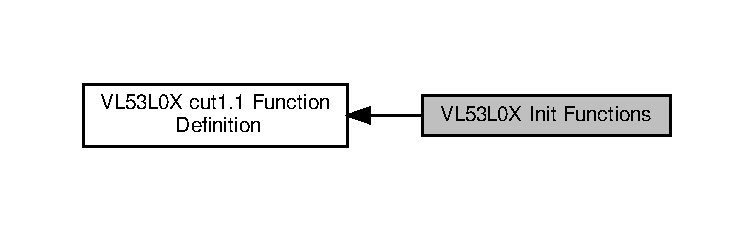
\includegraphics[width=350pt]{group__VL53L0X__init__group}
\end{center}
\end{figure}
\subsection*{Functions}
\begin{DoxyCompactItemize}
\item 
V\+L53\+L0\+X\+\_\+\+A\+PI V\+L53\+L0\+X\+\_\+\+Error \hyperlink{group__VL53L0X__init__group_ga7cb9d3ec8f6e74e921df2eeb600647d7}{V\+L53\+L0\+X\+\_\+\+Set\+Device\+Address} (\hyperlink{group__VL53L0X__platform__group_ga2d6405308b1dd524b462f1b8fb97d167}{V\+L53\+L0\+X\+\_\+\+D\+EV} Dev, \hyperlink{vl53l0x__types_8h_aba7bc1797add20fe3efdf37ced1182c5}{uint8\+\_\+t} Device\+Address)
\begin{DoxyCompactList}\small\item\em Set new device address. \end{DoxyCompactList}\item 
V\+L53\+L0\+X\+\_\+\+A\+PI V\+L53\+L0\+X\+\_\+\+Error \hyperlink{group__VL53L0X__init__group_gabb81d6ad638363d555a1b1b038b23354}{V\+L53\+L0\+X\+\_\+\+Data\+Init} (\hyperlink{group__VL53L0X__platform__group_ga2d6405308b1dd524b462f1b8fb97d167}{V\+L53\+L0\+X\+\_\+\+D\+EV} Dev)
\begin{DoxyCompactList}\small\item\em One time device initialization. \end{DoxyCompactList}\item 
V\+L53\+L0\+X\+\_\+\+A\+PI V\+L53\+L0\+X\+\_\+\+Error \hyperlink{group__VL53L0X__init__group_gabf9df2a66482932ebedab524ecedaaf1}{V\+L53\+L0\+X\+\_\+\+Set\+Tuning\+Setting\+Buffer} (\hyperlink{group__VL53L0X__platform__group_ga2d6405308b1dd524b462f1b8fb97d167}{V\+L53\+L0\+X\+\_\+\+D\+EV} Dev, \hyperlink{vl53l0x__types_8h_aba7bc1797add20fe3efdf37ced1182c5}{uint8\+\_\+t} $\ast$p\+Tuning\+Setting\+Buffer, \hyperlink{vl53l0x__types_8h_aba7bc1797add20fe3efdf37ced1182c5}{uint8\+\_\+t} Use\+Internal\+Tuning\+Settings)
\begin{DoxyCompactList}\small\item\em Set the tuning settings pointer. \end{DoxyCompactList}\item 
V\+L53\+L0\+X\+\_\+\+A\+PI V\+L53\+L0\+X\+\_\+\+Error \hyperlink{group__VL53L0X__init__group_ga6ecb2af8572433323cc3bff093bbf636}{V\+L53\+L0\+X\+\_\+\+Get\+Tuning\+Setting\+Buffer} (\hyperlink{group__VL53L0X__platform__group_ga2d6405308b1dd524b462f1b8fb97d167}{V\+L53\+L0\+X\+\_\+\+D\+EV} Dev, \hyperlink{vl53l0x__types_8h_aba7bc1797add20fe3efdf37ced1182c5}{uint8\+\_\+t} $\ast$$\ast$pp\+Tuning\+Setting\+Buffer, \hyperlink{vl53l0x__types_8h_aba7bc1797add20fe3efdf37ced1182c5}{uint8\+\_\+t} $\ast$p\+Use\+Internal\+Tuning\+Settings)
\begin{DoxyCompactList}\small\item\em Get the tuning settings pointer and the internal external switch value. \end{DoxyCompactList}\item 
V\+L53\+L0\+X\+\_\+\+A\+PI V\+L53\+L0\+X\+\_\+\+Error \hyperlink{group__VL53L0X__init__group_ga7cf27cba40b2f87dabdc5020aa567b77}{V\+L53\+L0\+X\+\_\+\+Static\+Init} (\hyperlink{group__VL53L0X__platform__group_ga2d6405308b1dd524b462f1b8fb97d167}{V\+L53\+L0\+X\+\_\+\+D\+EV} Dev)
\begin{DoxyCompactList}\small\item\em Do basic device init (and eventually patch loading) This function will change the V\+L53\+L0\+X\+\_\+\+State from V\+L53\+L0\+X\+\_\+\+S\+T\+A\+T\+E\+\_\+\+W\+A\+I\+T\+\_\+\+S\+T\+A\+T\+I\+C\+I\+N\+IT to V\+L53\+L0\+X\+\_\+\+S\+T\+A\+T\+E\+\_\+\+I\+D\+LE. In this stage all default setting will be applied. \end{DoxyCompactList}\item 
V\+L53\+L0\+X\+\_\+\+A\+PI V\+L53\+L0\+X\+\_\+\+Error \hyperlink{group__VL53L0X__init__group_ga079f2bafbcb26cb4ccf897bb835fcdc8}{V\+L53\+L0\+X\+\_\+\+Wait\+Device\+Booted} (\hyperlink{group__VL53L0X__platform__group_ga2d6405308b1dd524b462f1b8fb97d167}{V\+L53\+L0\+X\+\_\+\+D\+EV} Dev)
\begin{DoxyCompactList}\small\item\em Wait for device booted after chip enable (hardware standby) This function can be run only when V\+L53\+L0\+X\+\_\+\+State is V\+L53\+L0\+X\+\_\+\+S\+T\+A\+T\+E\+\_\+\+P\+O\+W\+E\+R\+D\+O\+WN. \end{DoxyCompactList}\item 
V\+L53\+L0\+X\+\_\+\+A\+PI V\+L53\+L0\+X\+\_\+\+Error \hyperlink{group__VL53L0X__init__group_gab089144ebdc35ee9abca9ca6c785561c}{V\+L53\+L0\+X\+\_\+\+Reset\+Device} (\hyperlink{group__VL53L0X__platform__group_ga2d6405308b1dd524b462f1b8fb97d167}{V\+L53\+L0\+X\+\_\+\+D\+EV} Dev)
\begin{DoxyCompactList}\small\item\em Do an hard reset or soft reset (depending on implementation) of the device  call of this function, device must be in same state as right after a power-\/up sequence.\+This function will change the V\+L53\+L0\+X\+\_\+\+State to V\+L53\+L0\+X\+\_\+\+S\+T\+A\+T\+E\+\_\+\+P\+O\+W\+E\+R\+D\+O\+WN. \end{DoxyCompactList}\end{DoxyCompactItemize}


\subsection{Detailed Description}
V\+L53\+L0X Init Functions. 



\subsection{Function Documentation}
\mbox{\Hypertarget{group__VL53L0X__init__group_gabb81d6ad638363d555a1b1b038b23354}\label{group__VL53L0X__init__group_gabb81d6ad638363d555a1b1b038b23354}} 
\index{V\+L53\+L0\+X Init Functions@{V\+L53\+L0\+X Init Functions}!V\+L53\+L0\+X\+\_\+\+Data\+Init@{V\+L53\+L0\+X\+\_\+\+Data\+Init}}
\index{V\+L53\+L0\+X\+\_\+\+Data\+Init@{V\+L53\+L0\+X\+\_\+\+Data\+Init}!V\+L53\+L0\+X Init Functions@{V\+L53\+L0\+X Init Functions}}
\subsubsection{\texorpdfstring{V\+L53\+L0\+X\+\_\+\+Data\+Init()}{VL53L0X\_DataInit()}}
{\footnotesize\ttfamily V\+L53\+L0\+X\+\_\+\+A\+PI V\+L53\+L0\+X\+\_\+\+Error V\+L53\+L0\+X\+\_\+\+Data\+Init (\begin{DoxyParamCaption}\item[{\hyperlink{group__VL53L0X__platform__group_ga2d6405308b1dd524b462f1b8fb97d167}{V\+L53\+L0\+X\+\_\+\+D\+EV}}]{Dev }\end{DoxyParamCaption})}



One time device initialization. 

To be called once and only once after device is brought out of reset (Chip enable) and booted see {\itshape \hyperlink{group__VL53L0X__init__group_ga079f2bafbcb26cb4ccf897bb835fcdc8}{V\+L53\+L0\+X\+\_\+\+Wait\+Device\+Booted()}} 

\begin{DoxyParagraph}{Function Description}
When not used after a fresh device \char`\"{}power up\char`\"{} or reset, it may return {\itshape \hyperlink{group__VL53L0X__define__Error__group_ga4bc7046c2d7a01b8c925af91d5325a65}{V\+L53\+L0\+X\+\_\+\+E\+R\+R\+O\+R\+\_\+\+C\+A\+L\+I\+B\+R\+A\+T\+I\+O\+N\+\_\+\+W\+A\+R\+N\+I\+NG}} meaning wrong calibration data may have been fetched from device that can result in ranging offset error~\newline
If application cannot execute device reset or need to run V\+L53\+L0\+X\+\_\+\+Data\+Init multiple time then it must ensure proper offset calibration saving and restore on its own by using {\itshape V\+L53\+L0\+X\+\_\+\+Get\+Offset\+Calibration\+Data()} on first power up and then {\itshape V\+L53\+L0\+X\+\_\+\+Set\+Offset\+Calibration\+Data()} in all subsequent init This function will change the V\+L53\+L0\+X\+\_\+\+State from V\+L53\+L0\+X\+\_\+\+S\+T\+A\+T\+E\+\_\+\+P\+O\+W\+E\+R\+D\+O\+WN to V\+L53\+L0\+X\+\_\+\+S\+T\+A\+T\+E\+\_\+\+W\+A\+I\+T\+\_\+\+S\+T\+A\+T\+I\+C\+I\+N\+IT.
\end{DoxyParagraph}
\begin{DoxyNote}{Note}
This function Access to the device
\end{DoxyNote}

\begin{DoxyParams}{Parameters}
{\em Dev} & Device Handle \\
\hline
\end{DoxyParams}
\begin{DoxyReturn}{Returns}
V\+L53\+L0\+X\+\_\+\+E\+R\+R\+O\+R\+\_\+\+N\+O\+NE Success 

\char`\"{}\+Other error code\char`\"{} See \+::\+V\+L53\+L0\+X\+\_\+\+Error 
\end{DoxyReturn}
\mbox{\Hypertarget{group__VL53L0X__init__group_ga6ecb2af8572433323cc3bff093bbf636}\label{group__VL53L0X__init__group_ga6ecb2af8572433323cc3bff093bbf636}} 
\index{V\+L53\+L0\+X Init Functions@{V\+L53\+L0\+X Init Functions}!V\+L53\+L0\+X\+\_\+\+Get\+Tuning\+Setting\+Buffer@{V\+L53\+L0\+X\+\_\+\+Get\+Tuning\+Setting\+Buffer}}
\index{V\+L53\+L0\+X\+\_\+\+Get\+Tuning\+Setting\+Buffer@{V\+L53\+L0\+X\+\_\+\+Get\+Tuning\+Setting\+Buffer}!V\+L53\+L0\+X Init Functions@{V\+L53\+L0\+X Init Functions}}
\subsubsection{\texorpdfstring{V\+L53\+L0\+X\+\_\+\+Get\+Tuning\+Setting\+Buffer()}{VL53L0X\_GetTuningSettingBuffer()}}
{\footnotesize\ttfamily V\+L53\+L0\+X\+\_\+\+A\+PI V\+L53\+L0\+X\+\_\+\+Error V\+L53\+L0\+X\+\_\+\+Get\+Tuning\+Setting\+Buffer (\begin{DoxyParamCaption}\item[{\hyperlink{group__VL53L0X__platform__group_ga2d6405308b1dd524b462f1b8fb97d167}{V\+L53\+L0\+X\+\_\+\+D\+EV}}]{Dev,  }\item[{\hyperlink{vl53l0x__types_8h_aba7bc1797add20fe3efdf37ced1182c5}{uint8\+\_\+t} $\ast$$\ast$}]{pp\+Tuning\+Setting\+Buffer,  }\item[{\hyperlink{vl53l0x__types_8h_aba7bc1797add20fe3efdf37ced1182c5}{uint8\+\_\+t} $\ast$}]{p\+Use\+Internal\+Tuning\+Settings }\end{DoxyParamCaption})}



Get the tuning settings pointer and the internal external switch value. 

This function is used to get the Tuning settings buffer pointer and the value. of the switch to select either external or internal tuning settings.

\begin{DoxyNote}{Note}
This function Access to the device
\end{DoxyNote}

\begin{DoxyParams}{Parameters}
{\em Dev} & Device Handle \\
\hline
{\em pp\+Tuning\+Setting\+Buffer} & Pointer to tuning settings buffer. \\
\hline
{\em p\+Use\+Internal\+Tuning\+Settings} & Pointer to store Use internal tuning settings value. \\
\hline
\end{DoxyParams}
\begin{DoxyReturn}{Returns}
V\+L53\+L0\+X\+\_\+\+E\+R\+R\+O\+R\+\_\+\+N\+O\+NE Success 

\char`\"{}\+Other error code\char`\"{} See \+::\+V\+L53\+L0\+X\+\_\+\+Error 
\end{DoxyReturn}
\mbox{\Hypertarget{group__VL53L0X__init__group_gab089144ebdc35ee9abca9ca6c785561c}\label{group__VL53L0X__init__group_gab089144ebdc35ee9abca9ca6c785561c}} 
\index{V\+L53\+L0\+X Init Functions@{V\+L53\+L0\+X Init Functions}!V\+L53\+L0\+X\+\_\+\+Reset\+Device@{V\+L53\+L0\+X\+\_\+\+Reset\+Device}}
\index{V\+L53\+L0\+X\+\_\+\+Reset\+Device@{V\+L53\+L0\+X\+\_\+\+Reset\+Device}!V\+L53\+L0\+X Init Functions@{V\+L53\+L0\+X Init Functions}}
\subsubsection{\texorpdfstring{V\+L53\+L0\+X\+\_\+\+Reset\+Device()}{VL53L0X\_ResetDevice()}}
{\footnotesize\ttfamily V\+L53\+L0\+X\+\_\+\+A\+PI V\+L53\+L0\+X\+\_\+\+Error V\+L53\+L0\+X\+\_\+\+Reset\+Device (\begin{DoxyParamCaption}\item[{\hyperlink{group__VL53L0X__platform__group_ga2d6405308b1dd524b462f1b8fb97d167}{V\+L53\+L0\+X\+\_\+\+D\+EV}}]{Dev }\end{DoxyParamCaption})}



Do an hard reset or soft reset (depending on implementation) of the device  call of this function, device must be in same state as right after a power-\/up sequence.\+This function will change the V\+L53\+L0\+X\+\_\+\+State to V\+L53\+L0\+X\+\_\+\+S\+T\+A\+T\+E\+\_\+\+P\+O\+W\+E\+R\+D\+O\+WN. 

\begin{DoxyNote}{Note}
This function Access to the device
\end{DoxyNote}

\begin{DoxyParams}{Parameters}
{\em Dev} & Device Handle \\
\hline
\end{DoxyParams}
\begin{DoxyReturn}{Returns}
V\+L53\+L0\+X\+\_\+\+E\+R\+R\+O\+R\+\_\+\+N\+O\+NE Success 

\char`\"{}\+Other error code\char`\"{} See \+::\+V\+L53\+L0\+X\+\_\+\+Error 
\end{DoxyReturn}
\mbox{\Hypertarget{group__VL53L0X__init__group_ga7cb9d3ec8f6e74e921df2eeb600647d7}\label{group__VL53L0X__init__group_ga7cb9d3ec8f6e74e921df2eeb600647d7}} 
\index{V\+L53\+L0\+X Init Functions@{V\+L53\+L0\+X Init Functions}!V\+L53\+L0\+X\+\_\+\+Set\+Device\+Address@{V\+L53\+L0\+X\+\_\+\+Set\+Device\+Address}}
\index{V\+L53\+L0\+X\+\_\+\+Set\+Device\+Address@{V\+L53\+L0\+X\+\_\+\+Set\+Device\+Address}!V\+L53\+L0\+X Init Functions@{V\+L53\+L0\+X Init Functions}}
\subsubsection{\texorpdfstring{V\+L53\+L0\+X\+\_\+\+Set\+Device\+Address()}{VL53L0X\_SetDeviceAddress()}}
{\footnotesize\ttfamily V\+L53\+L0\+X\+\_\+\+A\+PI V\+L53\+L0\+X\+\_\+\+Error V\+L53\+L0\+X\+\_\+\+Set\+Device\+Address (\begin{DoxyParamCaption}\item[{\hyperlink{group__VL53L0X__platform__group_ga2d6405308b1dd524b462f1b8fb97d167}{V\+L53\+L0\+X\+\_\+\+D\+EV}}]{Dev,  }\item[{\hyperlink{vl53l0x__types_8h_aba7bc1797add20fe3efdf37ced1182c5}{uint8\+\_\+t}}]{Device\+Address }\end{DoxyParamCaption})}



Set new device address. 

After completion the device will answer to the new address programmed. This function should be called when several devices are used in parallel before start programming the sensor. When a single device us used, there is no need to call this function.

\begin{DoxyNote}{Note}
This function Access to the device
\end{DoxyNote}

\begin{DoxyParams}{Parameters}
{\em Dev} & Device Handle \\
\hline
{\em Device\+Address} & \hyperlink{structThe}{The} new Device address \\
\hline
\end{DoxyParams}
\begin{DoxyReturn}{Returns}
V\+L53\+L0\+X\+\_\+\+E\+R\+R\+O\+R\+\_\+\+N\+O\+NE Success 

\char`\"{}\+Other error code\char`\"{} See \+::\+V\+L53\+L0\+X\+\_\+\+Error 
\end{DoxyReturn}
\mbox{\Hypertarget{group__VL53L0X__init__group_gabf9df2a66482932ebedab524ecedaaf1}\label{group__VL53L0X__init__group_gabf9df2a66482932ebedab524ecedaaf1}} 
\index{V\+L53\+L0\+X Init Functions@{V\+L53\+L0\+X Init Functions}!V\+L53\+L0\+X\+\_\+\+Set\+Tuning\+Setting\+Buffer@{V\+L53\+L0\+X\+\_\+\+Set\+Tuning\+Setting\+Buffer}}
\index{V\+L53\+L0\+X\+\_\+\+Set\+Tuning\+Setting\+Buffer@{V\+L53\+L0\+X\+\_\+\+Set\+Tuning\+Setting\+Buffer}!V\+L53\+L0\+X Init Functions@{V\+L53\+L0\+X Init Functions}}
\subsubsection{\texorpdfstring{V\+L53\+L0\+X\+\_\+\+Set\+Tuning\+Setting\+Buffer()}{VL53L0X\_SetTuningSettingBuffer()}}
{\footnotesize\ttfamily V\+L53\+L0\+X\+\_\+\+A\+PI V\+L53\+L0\+X\+\_\+\+Error V\+L53\+L0\+X\+\_\+\+Set\+Tuning\+Setting\+Buffer (\begin{DoxyParamCaption}\item[{\hyperlink{group__VL53L0X__platform__group_ga2d6405308b1dd524b462f1b8fb97d167}{V\+L53\+L0\+X\+\_\+\+D\+EV}}]{Dev,  }\item[{\hyperlink{vl53l0x__types_8h_aba7bc1797add20fe3efdf37ced1182c5}{uint8\+\_\+t} $\ast$}]{p\+Tuning\+Setting\+Buffer,  }\item[{\hyperlink{vl53l0x__types_8h_aba7bc1797add20fe3efdf37ced1182c5}{uint8\+\_\+t}}]{Use\+Internal\+Tuning\+Settings }\end{DoxyParamCaption})}



Set the tuning settings pointer. 

This function is used to specify the Tuning settings buffer to be used for a given device. \hyperlink{structThe}{The} buffer contains all the necessary data to permit the A\+PI to write tuning settings. This function permit to force the usage of either external or internal tuning settings.

\begin{DoxyNote}{Note}
This function Access to the device
\end{DoxyNote}

\begin{DoxyParams}{Parameters}
{\em Dev} & Device Handle \\
\hline
{\em p\+Tuning\+Setting\+Buffer} & Pointer to tuning settings buffer. \\
\hline
{\em Use\+Internal\+Tuning\+Settings} & Use internal tuning settings value. \\
\hline
\end{DoxyParams}
\begin{DoxyReturn}{Returns}
V\+L53\+L0\+X\+\_\+\+E\+R\+R\+O\+R\+\_\+\+N\+O\+NE Success 

\char`\"{}\+Other error code\char`\"{} See \+::\+V\+L53\+L0\+X\+\_\+\+Error 
\end{DoxyReturn}
\mbox{\Hypertarget{group__VL53L0X__init__group_ga7cf27cba40b2f87dabdc5020aa567b77}\label{group__VL53L0X__init__group_ga7cf27cba40b2f87dabdc5020aa567b77}} 
\index{V\+L53\+L0\+X Init Functions@{V\+L53\+L0\+X Init Functions}!V\+L53\+L0\+X\+\_\+\+Static\+Init@{V\+L53\+L0\+X\+\_\+\+Static\+Init}}
\index{V\+L53\+L0\+X\+\_\+\+Static\+Init@{V\+L53\+L0\+X\+\_\+\+Static\+Init}!V\+L53\+L0\+X Init Functions@{V\+L53\+L0\+X Init Functions}}
\subsubsection{\texorpdfstring{V\+L53\+L0\+X\+\_\+\+Static\+Init()}{VL53L0X\_StaticInit()}}
{\footnotesize\ttfamily V\+L53\+L0\+X\+\_\+\+A\+PI V\+L53\+L0\+X\+\_\+\+Error V\+L53\+L0\+X\+\_\+\+Static\+Init (\begin{DoxyParamCaption}\item[{\hyperlink{group__VL53L0X__platform__group_ga2d6405308b1dd524b462f1b8fb97d167}{V\+L53\+L0\+X\+\_\+\+D\+EV}}]{Dev }\end{DoxyParamCaption})}



Do basic device init (and eventually patch loading) This function will change the V\+L53\+L0\+X\+\_\+\+State from V\+L53\+L0\+X\+\_\+\+S\+T\+A\+T\+E\+\_\+\+W\+A\+I\+T\+\_\+\+S\+T\+A\+T\+I\+C\+I\+N\+IT to V\+L53\+L0\+X\+\_\+\+S\+T\+A\+T\+E\+\_\+\+I\+D\+LE. In this stage all default setting will be applied. 

\begin{DoxyNote}{Note}
This function Access to the device
\end{DoxyNote}

\begin{DoxyParams}{Parameters}
{\em Dev} & Device Handle \\
\hline
\end{DoxyParams}
\begin{DoxyReturn}{Returns}
V\+L53\+L0\+X\+\_\+\+E\+R\+R\+O\+R\+\_\+\+N\+O\+NE Success 

\char`\"{}\+Other error code\char`\"{} See \+::\+V\+L53\+L0\+X\+\_\+\+Error 
\end{DoxyReturn}
\mbox{\Hypertarget{group__VL53L0X__init__group_ga079f2bafbcb26cb4ccf897bb835fcdc8}\label{group__VL53L0X__init__group_ga079f2bafbcb26cb4ccf897bb835fcdc8}} 
\index{V\+L53\+L0\+X Init Functions@{V\+L53\+L0\+X Init Functions}!V\+L53\+L0\+X\+\_\+\+Wait\+Device\+Booted@{V\+L53\+L0\+X\+\_\+\+Wait\+Device\+Booted}}
\index{V\+L53\+L0\+X\+\_\+\+Wait\+Device\+Booted@{V\+L53\+L0\+X\+\_\+\+Wait\+Device\+Booted}!V\+L53\+L0\+X Init Functions@{V\+L53\+L0\+X Init Functions}}
\subsubsection{\texorpdfstring{V\+L53\+L0\+X\+\_\+\+Wait\+Device\+Booted()}{VL53L0X\_WaitDeviceBooted()}}
{\footnotesize\ttfamily V\+L53\+L0\+X\+\_\+\+A\+PI V\+L53\+L0\+X\+\_\+\+Error V\+L53\+L0\+X\+\_\+\+Wait\+Device\+Booted (\begin{DoxyParamCaption}\item[{\hyperlink{group__VL53L0X__platform__group_ga2d6405308b1dd524b462f1b8fb97d167}{V\+L53\+L0\+X\+\_\+\+D\+EV}}]{Dev }\end{DoxyParamCaption})}



Wait for device booted after chip enable (hardware standby) This function can be run only when V\+L53\+L0\+X\+\_\+\+State is V\+L53\+L0\+X\+\_\+\+S\+T\+A\+T\+E\+\_\+\+P\+O\+W\+E\+R\+D\+O\+WN. 

\begin{DoxyNote}{Note}
This function is not Implemented
\end{DoxyNote}

\begin{DoxyParams}{Parameters}
{\em Dev} & Device Handle \\
\hline
\end{DoxyParams}
\begin{DoxyReturn}{Returns}
V\+L53\+L0\+X\+\_\+\+E\+R\+R\+O\+R\+\_\+\+N\+O\+T\+\_\+\+I\+M\+P\+L\+E\+M\+E\+N\+T\+ED Not implemented 
\end{DoxyReturn}

\hypertarget{group__VL53L0X__parameters__group}{}\section{V\+L53\+L0X Parameters Functions}
\label{group__VL53L0X__parameters__group}\index{V\+L53\+L0\+X Parameters Functions@{V\+L53\+L0\+X Parameters Functions}}


Functions used to prepare and setup the device.  


Collaboration diagram for V\+L53\+L0X Parameters Functions\+:\nopagebreak
\begin{figure}[H]
\begin{center}
\leavevmode
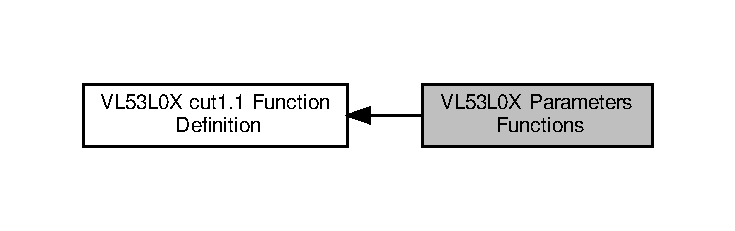
\includegraphics[width=350pt]{group__VL53L0X__parameters__group}
\end{center}
\end{figure}
\subsection*{Functions}
\begin{DoxyCompactItemize}
\item 
V\+L53\+L0\+X\+\_\+\+A\+PI V\+L53\+L0\+X\+\_\+\+Error \hyperlink{group__VL53L0X__parameters__group_ga2324960c4e2c54ab5d5788a51e985a86}{V\+L53\+L0\+X\+\_\+\+Set\+Device\+Parameters} (\hyperlink{group__VL53L0X__platform__group_ga2d6405308b1dd524b462f1b8fb97d167}{V\+L53\+L0\+X\+\_\+\+D\+EV} Dev, const \hyperlink{structVL53L0X__DeviceParameters__t}{V\+L53\+L0\+X\+\_\+\+Device\+Parameters\+\_\+t} $\ast$p\+Device\+Parameters)
\begin{DoxyCompactList}\small\item\em Prepare device for operation. \end{DoxyCompactList}\item 
V\+L53\+L0\+X\+\_\+\+A\+PI V\+L53\+L0\+X\+\_\+\+Error \hyperlink{group__VL53L0X__parameters__group_ga77d631bab7c544b6c8bcd725f224f05d}{V\+L53\+L0\+X\+\_\+\+Get\+Device\+Parameters} (\hyperlink{group__VL53L0X__platform__group_ga2d6405308b1dd524b462f1b8fb97d167}{V\+L53\+L0\+X\+\_\+\+D\+EV} Dev, \hyperlink{structVL53L0X__DeviceParameters__t}{V\+L53\+L0\+X\+\_\+\+Device\+Parameters\+\_\+t} $\ast$p\+Device\+Parameters)
\begin{DoxyCompactList}\small\item\em Retrieve current device parameters. \end{DoxyCompactList}\item 
V\+L53\+L0\+X\+\_\+\+A\+PI V\+L53\+L0\+X\+\_\+\+Error \hyperlink{group__VL53L0X__parameters__group_ga547bf7479b5ec799db4aafb7111271f7}{V\+L53\+L0\+X\+\_\+\+Set\+Device\+Mode} (\hyperlink{group__VL53L0X__platform__group_ga2d6405308b1dd524b462f1b8fb97d167}{V\+L53\+L0\+X\+\_\+\+D\+EV} Dev, V\+L53\+L0\+X\+\_\+\+Device\+Modes Device\+Mode)
\begin{DoxyCompactList}\small\item\em Set a new device mode. \end{DoxyCompactList}\item 
V\+L53\+L0\+X\+\_\+\+A\+PI V\+L53\+L0\+X\+\_\+\+Error \hyperlink{group__VL53L0X__parameters__group_ga228a691a1d324522523f4e7ff6f8c9bd}{V\+L53\+L0\+X\+\_\+\+Get\+Device\+Mode} (\hyperlink{group__VL53L0X__platform__group_ga2d6405308b1dd524b462f1b8fb97d167}{V\+L53\+L0\+X\+\_\+\+D\+EV} Dev, V\+L53\+L0\+X\+\_\+\+Device\+Modes $\ast$p\+Device\+Mode)
\begin{DoxyCompactList}\small\item\em Get current new device mode. \end{DoxyCompactList}\item 
V\+L53\+L0\+X\+\_\+\+A\+PI V\+L53\+L0\+X\+\_\+\+Error \hyperlink{group__VL53L0X__parameters__group_ga8efed262abe1ceff56edf7b3faa9bd86}{V\+L53\+L0\+X\+\_\+\+Set\+Range\+Fraction\+Enable} (\hyperlink{group__VL53L0X__platform__group_ga2d6405308b1dd524b462f1b8fb97d167}{V\+L53\+L0\+X\+\_\+\+D\+EV} Dev, \hyperlink{vl53l0x__types_8h_aba7bc1797add20fe3efdf37ced1182c5}{uint8\+\_\+t} Enable)
\begin{DoxyCompactList}\small\item\em Sets the resolution of range measurements. \end{DoxyCompactList}\item 
V\+L53\+L0\+X\+\_\+\+A\+PI V\+L53\+L0\+X\+\_\+\+Error \hyperlink{group__VL53L0X__parameters__group_gac339a9c68d173fda1319a98f17cba09c}{V\+L53\+L0\+X\+\_\+\+Get\+Fraction\+Enable} (\hyperlink{group__VL53L0X__platform__group_ga2d6405308b1dd524b462f1b8fb97d167}{V\+L53\+L0\+X\+\_\+\+D\+EV} Dev, \hyperlink{vl53l0x__types_8h_aba7bc1797add20fe3efdf37ced1182c5}{uint8\+\_\+t} $\ast$p\+Enable)
\begin{DoxyCompactList}\small\item\em Gets the fraction enable parameter indicating the resolution of range measurements. \end{DoxyCompactList}\item 
V\+L53\+L0\+X\+\_\+\+A\+PI V\+L53\+L0\+X\+\_\+\+Error \hyperlink{group__VL53L0X__parameters__group_ga6895ba3bdaff31cbce0f1dc2691eacd7}{V\+L53\+L0\+X\+\_\+\+Set\+Histogram\+Mode} (\hyperlink{group__VL53L0X__platform__group_ga2d6405308b1dd524b462f1b8fb97d167}{V\+L53\+L0\+X\+\_\+\+D\+EV} Dev, V\+L53\+L0\+X\+\_\+\+Histogram\+Modes Histogram\+Mode)
\begin{DoxyCompactList}\small\item\em Set a new Histogram mode. \end{DoxyCompactList}\item 
V\+L53\+L0\+X\+\_\+\+A\+PI V\+L53\+L0\+X\+\_\+\+Error \hyperlink{group__VL53L0X__parameters__group_gaea90e545569556a6e2f6e0bc3e3b92dd}{V\+L53\+L0\+X\+\_\+\+Get\+Histogram\+Mode} (\hyperlink{group__VL53L0X__platform__group_ga2d6405308b1dd524b462f1b8fb97d167}{V\+L53\+L0\+X\+\_\+\+D\+EV} Dev, V\+L53\+L0\+X\+\_\+\+Histogram\+Modes $\ast$p\+Histogram\+Mode)
\begin{DoxyCompactList}\small\item\em Get current new device mode. \end{DoxyCompactList}\item 
V\+L53\+L0\+X\+\_\+\+A\+PI V\+L53\+L0\+X\+\_\+\+Error \hyperlink{group__VL53L0X__parameters__group_gace59208a51f53cc3ab9bf834bdd2e36f}{V\+L53\+L0\+X\+\_\+\+Set\+Measurement\+Timing\+Budget\+Micro\+Seconds} (\hyperlink{group__VL53L0X__platform__group_ga2d6405308b1dd524b462f1b8fb97d167}{V\+L53\+L0\+X\+\_\+\+D\+EV} Dev, \hyperlink{vl53l0x__types_8h_a435d1572bf3f880d55459d9805097f62}{uint32\+\_\+t} Measurement\+Timing\+Budget\+Micro\+Seconds)
\begin{DoxyCompactList}\small\item\em Set Ranging Timing Budget in microseconds. \end{DoxyCompactList}\item 
V\+L53\+L0\+X\+\_\+\+A\+PI V\+L53\+L0\+X\+\_\+\+Error \hyperlink{group__VL53L0X__parameters__group_ga567e1870afa4cd7b050f2eb807168e1c}{V\+L53\+L0\+X\+\_\+\+Get\+Measurement\+Timing\+Budget\+Micro\+Seconds} (\hyperlink{group__VL53L0X__platform__group_ga2d6405308b1dd524b462f1b8fb97d167}{V\+L53\+L0\+X\+\_\+\+D\+EV} Dev, \hyperlink{vl53l0x__types_8h_a435d1572bf3f880d55459d9805097f62}{uint32\+\_\+t} $\ast$p\+Measurement\+Timing\+Budget\+Micro\+Seconds)
\begin{DoxyCompactList}\small\item\em Get Ranging Timing Budget in microseconds. \end{DoxyCompactList}\item 
V\+L53\+L0\+X\+\_\+\+A\+PI V\+L53\+L0\+X\+\_\+\+Error \hyperlink{group__VL53L0X__parameters__group_ga459e0031cf69d5eee71cb46bc8a3daec}{V\+L53\+L0\+X\+\_\+\+Get\+Vcsel\+Pulse\+Period} (\hyperlink{group__VL53L0X__platform__group_ga2d6405308b1dd524b462f1b8fb97d167}{V\+L53\+L0\+X\+\_\+\+D\+EV} Dev, V\+L53\+L0\+X\+\_\+\+Vcsel\+Period Vcsel\+Period\+Type, \hyperlink{vl53l0x__types_8h_aba7bc1797add20fe3efdf37ced1182c5}{uint8\+\_\+t} $\ast$p\+V\+C\+S\+E\+L\+Pulse\+Period)
\begin{DoxyCompactList}\small\item\em Gets the V\+C\+S\+EL pulse period. \end{DoxyCompactList}\item 
V\+L53\+L0\+X\+\_\+\+A\+PI V\+L53\+L0\+X\+\_\+\+Error \hyperlink{group__VL53L0X__parameters__group_ga64ade1f2ee420b6a7b55b744cc8e06f0}{V\+L53\+L0\+X\+\_\+\+Set\+Vcsel\+Pulse\+Period} (\hyperlink{group__VL53L0X__platform__group_ga2d6405308b1dd524b462f1b8fb97d167}{V\+L53\+L0\+X\+\_\+\+D\+EV} Dev, V\+L53\+L0\+X\+\_\+\+Vcsel\+Period Vcsel\+Period\+Type, \hyperlink{vl53l0x__types_8h_aba7bc1797add20fe3efdf37ced1182c5}{uint8\+\_\+t} V\+C\+S\+E\+L\+Pulse\+Period)
\begin{DoxyCompactList}\small\item\em Sets the V\+C\+S\+EL pulse period. \end{DoxyCompactList}\item 
V\+L53\+L0\+X\+\_\+\+A\+PI V\+L53\+L0\+X\+\_\+\+Error \hyperlink{group__VL53L0X__parameters__group_gab8893aac301ab753e99d3245753b4294}{V\+L53\+L0\+X\+\_\+\+Set\+Sequence\+Step\+Enable} (\hyperlink{group__VL53L0X__platform__group_ga2d6405308b1dd524b462f1b8fb97d167}{V\+L53\+L0\+X\+\_\+\+D\+EV} Dev, V\+L53\+L0\+X\+\_\+\+Sequence\+Step\+Id Sequence\+Step\+Id, \hyperlink{vl53l0x__types_8h_aba7bc1797add20fe3efdf37ced1182c5}{uint8\+\_\+t} Sequence\+Step\+Enabled)
\begin{DoxyCompactList}\small\item\em Sets the (on/off) state of a requested sequence step. \end{DoxyCompactList}\item 
V\+L53\+L0\+X\+\_\+\+A\+PI V\+L53\+L0\+X\+\_\+\+Error \hyperlink{group__VL53L0X__parameters__group_ga27047120f1ee506c3ddf07baed683b81}{V\+L53\+L0\+X\+\_\+\+Get\+Sequence\+Step\+Enable} (\hyperlink{group__VL53L0X__platform__group_ga2d6405308b1dd524b462f1b8fb97d167}{V\+L53\+L0\+X\+\_\+\+D\+EV} Dev, V\+L53\+L0\+X\+\_\+\+Sequence\+Step\+Id Sequence\+Step\+Id, \hyperlink{vl53l0x__types_8h_aba7bc1797add20fe3efdf37ced1182c5}{uint8\+\_\+t} $\ast$p\+Sequence\+Step\+Enabled)
\begin{DoxyCompactList}\small\item\em Gets the (on/off) state of a requested sequence step. \end{DoxyCompactList}\item 
V\+L53\+L0\+X\+\_\+\+A\+PI V\+L53\+L0\+X\+\_\+\+Error \hyperlink{group__VL53L0X__parameters__group_ga7fc642dea262d2853ac0e9f4bf7d9024}{V\+L53\+L0\+X\+\_\+\+Get\+Sequence\+Step\+Enables} (\hyperlink{group__VL53L0X__platform__group_ga2d6405308b1dd524b462f1b8fb97d167}{V\+L53\+L0\+X\+\_\+\+D\+EV} Dev, \hyperlink{structVL53L0X__SchedulerSequenceSteps__t}{V\+L53\+L0\+X\+\_\+\+Scheduler\+Sequence\+Steps\+\_\+t} $\ast$p\+Scheduler\+Sequence\+Steps)
\begin{DoxyCompactList}\small\item\em Gets the (on/off) state of all sequence steps. \end{DoxyCompactList}\item 
V\+L53\+L0\+X\+\_\+\+A\+PI V\+L53\+L0\+X\+\_\+\+Error \hyperlink{group__VL53L0X__parameters__group_ga14baa118af01991f4633f0090b437170}{V\+L53\+L0\+X\+\_\+\+Set\+Sequence\+Step\+Timeout} (\hyperlink{group__VL53L0X__platform__group_ga2d6405308b1dd524b462f1b8fb97d167}{V\+L53\+L0\+X\+\_\+\+D\+EV} Dev, V\+L53\+L0\+X\+\_\+\+Sequence\+Step\+Id Sequence\+Step\+Id, \hyperlink{vl53l0x__types_8h_afb910790161809fc76e1a274a6349384}{Fix\+Point1616\+\_\+t} Time\+Out\+Milli\+Secs)
\begin{DoxyCompactList}\small\item\em Sets the timeout of a requested sequence step. \end{DoxyCompactList}\item 
V\+L53\+L0\+X\+\_\+\+A\+PI V\+L53\+L0\+X\+\_\+\+Error \hyperlink{group__VL53L0X__parameters__group_gacac67612ceb128355f2bc7a4354a049f}{V\+L53\+L0\+X\+\_\+\+Get\+Sequence\+Step\+Timeout} (\hyperlink{group__VL53L0X__platform__group_ga2d6405308b1dd524b462f1b8fb97d167}{V\+L53\+L0\+X\+\_\+\+D\+EV} Dev, V\+L53\+L0\+X\+\_\+\+Sequence\+Step\+Id Sequence\+Step\+Id, \hyperlink{vl53l0x__types_8h_afb910790161809fc76e1a274a6349384}{Fix\+Point1616\+\_\+t} $\ast$p\+Time\+Out\+Milli\+Secs)
\begin{DoxyCompactList}\small\item\em Gets the timeout of a requested sequence step. \end{DoxyCompactList}\item 
V\+L53\+L0\+X\+\_\+\+A\+PI V\+L53\+L0\+X\+\_\+\+Error \hyperlink{group__VL53L0X__parameters__group_ga04e798f39db282735d534e36bae9b4e8}{V\+L53\+L0\+X\+\_\+\+Get\+Number\+Of\+Sequence\+Steps} (\hyperlink{group__VL53L0X__platform__group_ga2d6405308b1dd524b462f1b8fb97d167}{V\+L53\+L0\+X\+\_\+\+D\+EV} Dev, \hyperlink{vl53l0x__types_8h_aba7bc1797add20fe3efdf37ced1182c5}{uint8\+\_\+t} $\ast$p\+Number\+Of\+Sequence\+Steps)
\begin{DoxyCompactList}\small\item\em Gets number of sequence steps managed by the A\+PI. \end{DoxyCompactList}\item 
V\+L53\+L0\+X\+\_\+\+A\+PI V\+L53\+L0\+X\+\_\+\+Error \hyperlink{group__VL53L0X__parameters__group_ga42e44b3fe3ea7f999fd7da3b94aa023e}{V\+L53\+L0\+X\+\_\+\+Get\+Sequence\+Steps\+Info} (V\+L53\+L0\+X\+\_\+\+Sequence\+Step\+Id Sequence\+Step\+Id, char $\ast$p\+Sequence\+Steps\+String)
\begin{DoxyCompactList}\small\item\em Gets the name of a given sequence step. \end{DoxyCompactList}\item 
V\+L53\+L0\+X\+\_\+\+A\+PI V\+L53\+L0\+X\+\_\+\+Error \hyperlink{group__VL53L0X__parameters__group_gac702606aaf8be1f7dc39a309997f28bc}{V\+L53\+L0\+X\+\_\+\+Set\+Inter\+Measurement\+Period\+Milli\+Seconds} (\hyperlink{group__VL53L0X__platform__group_ga2d6405308b1dd524b462f1b8fb97d167}{V\+L53\+L0\+X\+\_\+\+D\+EV} Dev, \hyperlink{vl53l0x__types_8h_a435d1572bf3f880d55459d9805097f62}{uint32\+\_\+t} Inter\+Measurement\+Period\+Milli\+Seconds)
\item 
V\+L53\+L0\+X\+\_\+\+A\+PI V\+L53\+L0\+X\+\_\+\+Error \hyperlink{group__VL53L0X__parameters__group_ga409fed78170c0ff606a125e514351324}{V\+L53\+L0\+X\+\_\+\+Get\+Inter\+Measurement\+Period\+Milli\+Seconds} (\hyperlink{group__VL53L0X__platform__group_ga2d6405308b1dd524b462f1b8fb97d167}{V\+L53\+L0\+X\+\_\+\+D\+EV} Dev, \hyperlink{vl53l0x__types_8h_a435d1572bf3f880d55459d9805097f62}{uint32\+\_\+t} $\ast$p\+Inter\+Measurement\+Period\+Milli\+Seconds)
\item 
V\+L53\+L0\+X\+\_\+\+A\+PI V\+L53\+L0\+X\+\_\+\+Error \hyperlink{group__VL53L0X__parameters__group_ga312b049fa776bc7a83502792a26a84d3}{V\+L53\+L0\+X\+\_\+\+Set\+X\+Talk\+Compensation\+Enable} (\hyperlink{group__VL53L0X__platform__group_ga2d6405308b1dd524b462f1b8fb97d167}{V\+L53\+L0\+X\+\_\+\+D\+EV} Dev, \hyperlink{vl53l0x__types_8h_aba7bc1797add20fe3efdf37ced1182c5}{uint8\+\_\+t} X\+Talk\+Compensation\+Enable)
\begin{DoxyCompactList}\small\item\em Enable/\+Disable Cross talk compensation feature. \end{DoxyCompactList}\item 
V\+L53\+L0\+X\+\_\+\+A\+PI V\+L53\+L0\+X\+\_\+\+Error \hyperlink{group__VL53L0X__parameters__group_gae0cd0ec86a3dd0270fb57587c49ac822}{V\+L53\+L0\+X\+\_\+\+Get\+X\+Talk\+Compensation\+Enable} (\hyperlink{group__VL53L0X__platform__group_ga2d6405308b1dd524b462f1b8fb97d167}{V\+L53\+L0\+X\+\_\+\+D\+EV} Dev, \hyperlink{vl53l0x__types_8h_aba7bc1797add20fe3efdf37ced1182c5}{uint8\+\_\+t} $\ast$p\+X\+Talk\+Compensation\+Enable)
\begin{DoxyCompactList}\small\item\em Get Cross talk compensation rate. \end{DoxyCompactList}\item 
V\+L53\+L0\+X\+\_\+\+A\+PI V\+L53\+L0\+X\+\_\+\+Error \hyperlink{group__VL53L0X__parameters__group_ga5a9549bdb784e68ef58663c21542f7ad}{V\+L53\+L0\+X\+\_\+\+Set\+X\+Talk\+Compensation\+Rate\+Mega\+Cps} (\hyperlink{group__VL53L0X__platform__group_ga2d6405308b1dd524b462f1b8fb97d167}{V\+L53\+L0\+X\+\_\+\+D\+EV} Dev, \hyperlink{vl53l0x__types_8h_afb910790161809fc76e1a274a6349384}{Fix\+Point1616\+\_\+t} X\+Talk\+Compensation\+Rate\+Mega\+Cps)
\begin{DoxyCompactList}\small\item\em Set Cross talk compensation rate. \end{DoxyCompactList}\item 
V\+L53\+L0\+X\+\_\+\+A\+PI V\+L53\+L0\+X\+\_\+\+Error \hyperlink{group__VL53L0X__parameters__group_ga64f96b1cd03b06e46253d4ff3230bc18}{V\+L53\+L0\+X\+\_\+\+Get\+X\+Talk\+Compensation\+Rate\+Mega\+Cps} (\hyperlink{group__VL53L0X__platform__group_ga2d6405308b1dd524b462f1b8fb97d167}{V\+L53\+L0\+X\+\_\+\+D\+EV} Dev, \hyperlink{vl53l0x__types_8h_afb910790161809fc76e1a274a6349384}{Fix\+Point1616\+\_\+t} $\ast$p\+X\+Talk\+Compensation\+Rate\+Mega\+Cps)
\begin{DoxyCompactList}\small\item\em Get Cross talk compensation rate. \end{DoxyCompactList}\item 
V\+L53\+L0\+X\+\_\+\+A\+PI V\+L53\+L0\+X\+\_\+\+Error \hyperlink{group__VL53L0X__parameters__group_ga83f7b83f76eaed0fdb4ea2034c3a9a21}{V\+L53\+L0\+X\+\_\+\+Set\+Ref\+Calibration} (\hyperlink{group__VL53L0X__platform__group_ga2d6405308b1dd524b462f1b8fb97d167}{V\+L53\+L0\+X\+\_\+\+D\+EV} Dev, \hyperlink{vl53l0x__types_8h_aba7bc1797add20fe3efdf37ced1182c5}{uint8\+\_\+t} Vhv\+Settings, \hyperlink{vl53l0x__types_8h_aba7bc1797add20fe3efdf37ced1182c5}{uint8\+\_\+t} Phase\+Cal)
\begin{DoxyCompactList}\small\item\em Set Reference Calibration Parameters. \end{DoxyCompactList}\item 
V\+L53\+L0\+X\+\_\+\+A\+PI V\+L53\+L0\+X\+\_\+\+Error \hyperlink{group__VL53L0X__parameters__group_ga5dc1b02f59fb47477184354975f169b6}{V\+L53\+L0\+X\+\_\+\+Get\+Ref\+Calibration} (\hyperlink{group__VL53L0X__platform__group_ga2d6405308b1dd524b462f1b8fb97d167}{V\+L53\+L0\+X\+\_\+\+D\+EV} Dev, \hyperlink{vl53l0x__types_8h_aba7bc1797add20fe3efdf37ced1182c5}{uint8\+\_\+t} $\ast$p\+Vhv\+Settings, \hyperlink{vl53l0x__types_8h_aba7bc1797add20fe3efdf37ced1182c5}{uint8\+\_\+t} $\ast$p\+Phase\+Cal)
\begin{DoxyCompactList}\small\item\em Get Reference Calibration Parameters. \end{DoxyCompactList}\item 
V\+L53\+L0\+X\+\_\+\+A\+PI V\+L53\+L0\+X\+\_\+\+Error \hyperlink{group__VL53L0X__parameters__group_ga96302da749e35322c0f031037aa457e1}{V\+L53\+L0\+X\+\_\+\+Get\+Number\+Of\+Limit\+Check} (\hyperlink{vl53l0x__types_8h_a273cf69d639a59973b6019625df33e30}{uint16\+\_\+t} $\ast$p\+Number\+Of\+Limit\+Check)
\begin{DoxyCompactList}\small\item\em Get the number of the check limit managed by a given Device. \end{DoxyCompactList}\item 
V\+L53\+L0\+X\+\_\+\+A\+PI V\+L53\+L0\+X\+\_\+\+Error \hyperlink{group__VL53L0X__parameters__group_ga4155c6a50a3eaf215d686759022a68f8}{V\+L53\+L0\+X\+\_\+\+Get\+Limit\+Check\+Info} (\hyperlink{group__VL53L0X__platform__group_ga2d6405308b1dd524b462f1b8fb97d167}{V\+L53\+L0\+X\+\_\+\+D\+EV} Dev, \hyperlink{vl53l0x__types_8h_a273cf69d639a59973b6019625df33e30}{uint16\+\_\+t} Limit\+Check\+Id, char $\ast$p\+Limit\+Check\+String)
\begin{DoxyCompactList}\small\item\em Return a description string for a given limit check number. \end{DoxyCompactList}\item 
V\+L53\+L0\+X\+\_\+\+A\+PI V\+L53\+L0\+X\+\_\+\+Error \hyperlink{group__VL53L0X__parameters__group_gab2edaef078d47dc9cac152d0e23493e9}{V\+L53\+L0\+X\+\_\+\+Get\+Limit\+Check\+Status} (\hyperlink{group__VL53L0X__platform__group_ga2d6405308b1dd524b462f1b8fb97d167}{V\+L53\+L0\+X\+\_\+\+D\+EV} Dev, \hyperlink{vl53l0x__types_8h_a273cf69d639a59973b6019625df33e30}{uint16\+\_\+t} Limit\+Check\+Id, \hyperlink{vl53l0x__types_8h_aba7bc1797add20fe3efdf37ced1182c5}{uint8\+\_\+t} $\ast$p\+Limit\+Check\+Status)
\begin{DoxyCompactList}\small\item\em Return a the Status of the specified check limit. \end{DoxyCompactList}\item 
V\+L53\+L0\+X\+\_\+\+A\+PI V\+L53\+L0\+X\+\_\+\+Error \hyperlink{group__VL53L0X__parameters__group_ga356967db0182329895ed339c70ad21af}{V\+L53\+L0\+X\+\_\+\+Set\+Limit\+Check\+Enable} (\hyperlink{group__VL53L0X__platform__group_ga2d6405308b1dd524b462f1b8fb97d167}{V\+L53\+L0\+X\+\_\+\+D\+EV} Dev, \hyperlink{vl53l0x__types_8h_a273cf69d639a59973b6019625df33e30}{uint16\+\_\+t} Limit\+Check\+Id, \hyperlink{vl53l0x__types_8h_aba7bc1797add20fe3efdf37ced1182c5}{uint8\+\_\+t} Limit\+Check\+Enable)
\begin{DoxyCompactList}\small\item\em Enable/\+Disable a specific limit check. \end{DoxyCompactList}\item 
V\+L53\+L0\+X\+\_\+\+A\+PI V\+L53\+L0\+X\+\_\+\+Error \hyperlink{group__VL53L0X__parameters__group_gafc13b35a676124eb56c43dfaf75fb510}{V\+L53\+L0\+X\+\_\+\+Get\+Limit\+Check\+Enable} (\hyperlink{group__VL53L0X__platform__group_ga2d6405308b1dd524b462f1b8fb97d167}{V\+L53\+L0\+X\+\_\+\+D\+EV} Dev, \hyperlink{vl53l0x__types_8h_a273cf69d639a59973b6019625df33e30}{uint16\+\_\+t} Limit\+Check\+Id, \hyperlink{vl53l0x__types_8h_aba7bc1797add20fe3efdf37ced1182c5}{uint8\+\_\+t} $\ast$p\+Limit\+Check\+Enable)
\begin{DoxyCompactList}\small\item\em Get specific limit check enable state. \end{DoxyCompactList}\item 
V\+L53\+L0\+X\+\_\+\+A\+PI V\+L53\+L0\+X\+\_\+\+Error \hyperlink{group__VL53L0X__parameters__group_ga5d311e2420317876030bc6caad01ea90}{V\+L53\+L0\+X\+\_\+\+Set\+Limit\+Check\+Value} (\hyperlink{group__VL53L0X__platform__group_ga2d6405308b1dd524b462f1b8fb97d167}{V\+L53\+L0\+X\+\_\+\+D\+EV} Dev, \hyperlink{vl53l0x__types_8h_a273cf69d639a59973b6019625df33e30}{uint16\+\_\+t} Limit\+Check\+Id, \hyperlink{vl53l0x__types_8h_afb910790161809fc76e1a274a6349384}{Fix\+Point1616\+\_\+t} Limit\+Check\+Value)
\begin{DoxyCompactList}\small\item\em Set a specific limit check value. \end{DoxyCompactList}\item 
V\+L53\+L0\+X\+\_\+\+A\+PI V\+L53\+L0\+X\+\_\+\+Error \hyperlink{group__VL53L0X__parameters__group_ga032fdca6d2bcb68621d4c0ed98d71e1a}{V\+L53\+L0\+X\+\_\+\+Get\+Limit\+Check\+Value} (\hyperlink{group__VL53L0X__platform__group_ga2d6405308b1dd524b462f1b8fb97d167}{V\+L53\+L0\+X\+\_\+\+D\+EV} Dev, \hyperlink{vl53l0x__types_8h_a273cf69d639a59973b6019625df33e30}{uint16\+\_\+t} Limit\+Check\+Id, \hyperlink{vl53l0x__types_8h_afb910790161809fc76e1a274a6349384}{Fix\+Point1616\+\_\+t} $\ast$p\+Limit\+Check\+Value)
\begin{DoxyCompactList}\small\item\em Get a specific limit check value. \end{DoxyCompactList}\item 
V\+L53\+L0\+X\+\_\+\+A\+PI V\+L53\+L0\+X\+\_\+\+Error \hyperlink{group__VL53L0X__parameters__group_ga5eba639cd2fe07d87a44f372b8c92e33}{V\+L53\+L0\+X\+\_\+\+Get\+Limit\+Check\+Current} (\hyperlink{group__VL53L0X__platform__group_ga2d6405308b1dd524b462f1b8fb97d167}{V\+L53\+L0\+X\+\_\+\+D\+EV} Dev, \hyperlink{vl53l0x__types_8h_a273cf69d639a59973b6019625df33e30}{uint16\+\_\+t} Limit\+Check\+Id, \hyperlink{vl53l0x__types_8h_afb910790161809fc76e1a274a6349384}{Fix\+Point1616\+\_\+t} $\ast$p\+Limit\+Check\+Current)
\begin{DoxyCompactList}\small\item\em Get the current value of the signal used for the limit check. \end{DoxyCompactList}\item 
V\+L53\+L0\+X\+\_\+\+A\+PI V\+L53\+L0\+X\+\_\+\+Error \hyperlink{group__VL53L0X__parameters__group_ga2ccb1408fe78f038ad34ffe5ab29cd39}{V\+L53\+L0\+X\+\_\+\+Set\+Wrap\+Around\+Check\+Enable} (\hyperlink{group__VL53L0X__platform__group_ga2d6405308b1dd524b462f1b8fb97d167}{V\+L53\+L0\+X\+\_\+\+D\+EV} Dev, \hyperlink{vl53l0x__types_8h_aba7bc1797add20fe3efdf37ced1182c5}{uint8\+\_\+t} Wrap\+Around\+Check\+Enable)
\begin{DoxyCompactList}\small\item\em Enable (or disable) Wrap around Check. \end{DoxyCompactList}\item 
V\+L53\+L0\+X\+\_\+\+A\+PI V\+L53\+L0\+X\+\_\+\+Error \hyperlink{group__VL53L0X__parameters__group_ga06cb130fc71a8c207d60af069b062725}{V\+L53\+L0\+X\+\_\+\+Get\+Wrap\+Around\+Check\+Enable} (\hyperlink{group__VL53L0X__platform__group_ga2d6405308b1dd524b462f1b8fb97d167}{V\+L53\+L0\+X\+\_\+\+D\+EV} Dev, \hyperlink{vl53l0x__types_8h_aba7bc1797add20fe3efdf37ced1182c5}{uint8\+\_\+t} $\ast$p\+Wrap\+Around\+Check\+Enable)
\begin{DoxyCompactList}\small\item\em Get setup of Wrap around Check. \end{DoxyCompactList}\item 
V\+L53\+L0\+X\+\_\+\+A\+PI V\+L53\+L0\+X\+\_\+\+Error \hyperlink{group__VL53L0X__parameters__group_ga3cf3ba12ba6b6db8ac0cfc6e756b87c1}{V\+L53\+L0\+X\+\_\+\+Set\+Dmax\+Cal\+Parameters} (\hyperlink{group__VL53L0X__platform__group_ga2d6405308b1dd524b462f1b8fb97d167}{V\+L53\+L0\+X\+\_\+\+D\+EV} Dev, \hyperlink{vl53l0x__types_8h_a273cf69d639a59973b6019625df33e30}{uint16\+\_\+t} Range\+Milli\+Meter, \hyperlink{vl53l0x__types_8h_afb910790161809fc76e1a274a6349384}{Fix\+Point1616\+\_\+t} Signal\+Rate\+Rtn\+Mega\+Cps)
\begin{DoxyCompactList}\small\item\em Set Dmax Calibration Parameters for a given device When one of the parameter is zero, this function will get parameter from N\+VM. \end{DoxyCompactList}\item 
V\+L53\+L0\+X\+\_\+\+A\+PI V\+L53\+L0\+X\+\_\+\+Error \hyperlink{group__VL53L0X__parameters__group_ga8e3f50afe785be486061bc30eb86129e}{V\+L53\+L0\+X\+\_\+\+Get\+Dmax\+Cal\+Parameters} (\hyperlink{group__VL53L0X__platform__group_ga2d6405308b1dd524b462f1b8fb97d167}{V\+L53\+L0\+X\+\_\+\+D\+EV} Dev, \hyperlink{vl53l0x__types_8h_a273cf69d639a59973b6019625df33e30}{uint16\+\_\+t} $\ast$p\+Range\+Milli\+Meter, \hyperlink{vl53l0x__types_8h_afb910790161809fc76e1a274a6349384}{Fix\+Point1616\+\_\+t} $\ast$p\+Signal\+Rate\+Rtn\+Mega\+Cps)
\begin{DoxyCompactList}\small\item\em Get Dmax Calibration Parameters for a given device. \end{DoxyCompactList}\end{DoxyCompactItemize}


\subsection{Detailed Description}
Functions used to prepare and setup the device. 



\subsection{Function Documentation}
\mbox{\Hypertarget{group__VL53L0X__parameters__group_ga228a691a1d324522523f4e7ff6f8c9bd}\label{group__VL53L0X__parameters__group_ga228a691a1d324522523f4e7ff6f8c9bd}} 
\index{V\+L53\+L0\+X Parameters Functions@{V\+L53\+L0\+X Parameters Functions}!V\+L53\+L0\+X\+\_\+\+Get\+Device\+Mode@{V\+L53\+L0\+X\+\_\+\+Get\+Device\+Mode}}
\index{V\+L53\+L0\+X\+\_\+\+Get\+Device\+Mode@{V\+L53\+L0\+X\+\_\+\+Get\+Device\+Mode}!V\+L53\+L0\+X Parameters Functions@{V\+L53\+L0\+X Parameters Functions}}
\subsubsection{\texorpdfstring{V\+L53\+L0\+X\+\_\+\+Get\+Device\+Mode()}{VL53L0X\_GetDeviceMode()}}
{\footnotesize\ttfamily V\+L53\+L0\+X\+\_\+\+A\+PI V\+L53\+L0\+X\+\_\+\+Error V\+L53\+L0\+X\+\_\+\+Get\+Device\+Mode (\begin{DoxyParamCaption}\item[{\hyperlink{group__VL53L0X__platform__group_ga2d6405308b1dd524b462f1b8fb97d167}{V\+L53\+L0\+X\+\_\+\+D\+EV}}]{Dev,  }\item[{V\+L53\+L0\+X\+\_\+\+Device\+Modes $\ast$}]{p\+Device\+Mode }\end{DoxyParamCaption})}



Get current new device mode. 

\begin{DoxyParagraph}{Function Description}
Get actual mode of the device(ranging, histogram ...)
\end{DoxyParagraph}
\begin{DoxyNote}{Note}
This function doesn\textquotesingle{}t Access to the device
\end{DoxyNote}

\begin{DoxyParams}{Parameters}
{\em Dev} & Device Handle \\
\hline
{\em p\+Device\+Mode} & Pointer to current apply mode value Valid values are\+: V\+L53\+L0\+X\+\_\+\+D\+E\+V\+I\+C\+E\+M\+O\+D\+E\+\_\+\+S\+I\+N\+G\+L\+E\+\_\+\+R\+A\+N\+G\+I\+NG V\+L53\+L0\+X\+\_\+\+D\+E\+V\+I\+C\+E\+M\+O\+D\+E\+\_\+\+C\+O\+N\+T\+I\+N\+U\+O\+U\+S\+\_\+\+R\+A\+N\+G\+I\+NG V\+L53\+L0\+X\+\_\+\+D\+E\+V\+I\+C\+E\+M\+O\+D\+E\+\_\+\+C\+O\+N\+T\+I\+N\+U\+O\+U\+S\+\_\+\+T\+I\+M\+E\+D\+\_\+\+R\+A\+N\+G\+I\+NG V\+L53\+L0\+X\+\_\+\+D\+E\+V\+I\+C\+E\+M\+O\+D\+E\+\_\+\+S\+I\+N\+G\+L\+E\+\_\+\+H\+I\+S\+T\+O\+G\+R\+AM V\+L53\+L0\+X\+\_\+\+H\+I\+S\+T\+O\+G\+R\+A\+M\+M\+O\+D\+E\+\_\+\+R\+E\+F\+E\+R\+E\+N\+C\+E\+\_\+\+O\+N\+LY V\+L53\+L0\+X\+\_\+\+H\+I\+S\+T\+O\+G\+R\+A\+M\+M\+O\+D\+E\+\_\+\+R\+E\+T\+U\+R\+N\+\_\+\+O\+N\+LY V\+L53\+L0\+X\+\_\+\+H\+I\+S\+T\+O\+G\+R\+A\+M\+M\+O\+D\+E\+\_\+\+B\+O\+TH\\
\hline
\end{DoxyParams}
\begin{DoxyReturn}{Returns}
V\+L53\+L0\+X\+\_\+\+E\+R\+R\+O\+R\+\_\+\+N\+O\+NE Success 

V\+L53\+L0\+X\+\_\+\+E\+R\+R\+O\+R\+\_\+\+M\+O\+D\+E\+\_\+\+N\+O\+T\+\_\+\+S\+U\+P\+P\+O\+R\+T\+ED This error occurs when Device\+Mode is not in the supported list 
\end{DoxyReturn}
\mbox{\Hypertarget{group__VL53L0X__parameters__group_ga77d631bab7c544b6c8bcd725f224f05d}\label{group__VL53L0X__parameters__group_ga77d631bab7c544b6c8bcd725f224f05d}} 
\index{V\+L53\+L0\+X Parameters Functions@{V\+L53\+L0\+X Parameters Functions}!V\+L53\+L0\+X\+\_\+\+Get\+Device\+Parameters@{V\+L53\+L0\+X\+\_\+\+Get\+Device\+Parameters}}
\index{V\+L53\+L0\+X\+\_\+\+Get\+Device\+Parameters@{V\+L53\+L0\+X\+\_\+\+Get\+Device\+Parameters}!V\+L53\+L0\+X Parameters Functions@{V\+L53\+L0\+X Parameters Functions}}
\subsubsection{\texorpdfstring{V\+L53\+L0\+X\+\_\+\+Get\+Device\+Parameters()}{VL53L0X\_GetDeviceParameters()}}
{\footnotesize\ttfamily V\+L53\+L0\+X\+\_\+\+A\+PI V\+L53\+L0\+X\+\_\+\+Error V\+L53\+L0\+X\+\_\+\+Get\+Device\+Parameters (\begin{DoxyParamCaption}\item[{\hyperlink{group__VL53L0X__platform__group_ga2d6405308b1dd524b462f1b8fb97d167}{V\+L53\+L0\+X\+\_\+\+D\+EV}}]{Dev,  }\item[{\hyperlink{structVL53L0X__DeviceParameters__t}{V\+L53\+L0\+X\+\_\+\+Device\+Parameters\+\_\+t} $\ast$}]{p\+Device\+Parameters }\end{DoxyParamCaption})}



Retrieve current device parameters. 

\begin{DoxyParagraph}{Function Description}
Get actual parameters of the device \begin{DoxyItemize}
\item Then start ranging operation.\end{DoxyItemize}

\end{DoxyParagraph}
\begin{DoxyNote}{Note}
This function Access to the device
\end{DoxyNote}

\begin{DoxyParams}{Parameters}
{\em Dev} & Device Handle \\
\hline
{\em p\+Device\+Parameters} & Pointer to store current device parameters. \\
\hline
\end{DoxyParams}
\begin{DoxyReturn}{Returns}
V\+L53\+L0\+X\+\_\+\+E\+R\+R\+O\+R\+\_\+\+N\+O\+NE Success 

\char`\"{}\+Other error code\char`\"{} See \+::\+V\+L53\+L0\+X\+\_\+\+Error 
\end{DoxyReturn}
\mbox{\Hypertarget{group__VL53L0X__parameters__group_ga8e3f50afe785be486061bc30eb86129e}\label{group__VL53L0X__parameters__group_ga8e3f50afe785be486061bc30eb86129e}} 
\index{V\+L53\+L0\+X Parameters Functions@{V\+L53\+L0\+X Parameters Functions}!V\+L53\+L0\+X\+\_\+\+Get\+Dmax\+Cal\+Parameters@{V\+L53\+L0\+X\+\_\+\+Get\+Dmax\+Cal\+Parameters}}
\index{V\+L53\+L0\+X\+\_\+\+Get\+Dmax\+Cal\+Parameters@{V\+L53\+L0\+X\+\_\+\+Get\+Dmax\+Cal\+Parameters}!V\+L53\+L0\+X Parameters Functions@{V\+L53\+L0\+X Parameters Functions}}
\subsubsection{\texorpdfstring{V\+L53\+L0\+X\+\_\+\+Get\+Dmax\+Cal\+Parameters()}{VL53L0X\_GetDmaxCalParameters()}}
{\footnotesize\ttfamily V\+L53\+L0\+X\+\_\+\+A\+PI V\+L53\+L0\+X\+\_\+\+Error V\+L53\+L0\+X\+\_\+\+Get\+Dmax\+Cal\+Parameters (\begin{DoxyParamCaption}\item[{\hyperlink{group__VL53L0X__platform__group_ga2d6405308b1dd524b462f1b8fb97d167}{V\+L53\+L0\+X\+\_\+\+D\+EV}}]{Dev,  }\item[{\hyperlink{vl53l0x__types_8h_a273cf69d639a59973b6019625df33e30}{uint16\+\_\+t} $\ast$}]{p\+Range\+Milli\+Meter,  }\item[{\hyperlink{vl53l0x__types_8h_afb910790161809fc76e1a274a6349384}{Fix\+Point1616\+\_\+t} $\ast$}]{p\+Signal\+Rate\+Rtn\+Mega\+Cps }\end{DoxyParamCaption})}



Get Dmax Calibration Parameters for a given device. 

\begin{DoxyNote}{Note}
This function Access to the device
\end{DoxyNote}

\begin{DoxyParams}{Parameters}
{\em Dev} & Device Handle \\
\hline
{\em p\+Range\+Milli\+Meter} & Pointer to Calibration Distance \\
\hline
{\em p\+Signal\+Rate\+Rtn\+Mega\+Cps} & Pointer to Signal rate return \\
\hline
\end{DoxyParams}
\begin{DoxyReturn}{Returns}
V\+L53\+L0\+X\+\_\+\+E\+R\+R\+O\+R\+\_\+\+N\+O\+NE Success 

\char`\"{}\+Other error code\char`\"{} See \+::\+V\+L53\+L0\+X\+\_\+\+Error 
\end{DoxyReturn}
\mbox{\Hypertarget{group__VL53L0X__parameters__group_gac339a9c68d173fda1319a98f17cba09c}\label{group__VL53L0X__parameters__group_gac339a9c68d173fda1319a98f17cba09c}} 
\index{V\+L53\+L0\+X Parameters Functions@{V\+L53\+L0\+X Parameters Functions}!V\+L53\+L0\+X\+\_\+\+Get\+Fraction\+Enable@{V\+L53\+L0\+X\+\_\+\+Get\+Fraction\+Enable}}
\index{V\+L53\+L0\+X\+\_\+\+Get\+Fraction\+Enable@{V\+L53\+L0\+X\+\_\+\+Get\+Fraction\+Enable}!V\+L53\+L0\+X Parameters Functions@{V\+L53\+L0\+X Parameters Functions}}
\subsubsection{\texorpdfstring{V\+L53\+L0\+X\+\_\+\+Get\+Fraction\+Enable()}{VL53L0X\_GetFractionEnable()}}
{\footnotesize\ttfamily V\+L53\+L0\+X\+\_\+\+A\+PI V\+L53\+L0\+X\+\_\+\+Error V\+L53\+L0\+X\+\_\+\+Get\+Fraction\+Enable (\begin{DoxyParamCaption}\item[{\hyperlink{group__VL53L0X__platform__group_ga2d6405308b1dd524b462f1b8fb97d167}{V\+L53\+L0\+X\+\_\+\+D\+EV}}]{Dev,  }\item[{\hyperlink{vl53l0x__types_8h_aba7bc1797add20fe3efdf37ced1182c5}{uint8\+\_\+t} $\ast$}]{p\+Enable }\end{DoxyParamCaption})}



Gets the fraction enable parameter indicating the resolution of range measurements. 

\begin{DoxyParagraph}{Function Description}
Gets the fraction enable state, which translates to the resolution of range measurements as follows \+:Enabled\+:=0.\+25mm resolution, Not Enabled\+:=1mm resolution.
\end{DoxyParagraph}
\begin{DoxyNote}{Note}
This function Accesses the device
\end{DoxyNote}

\begin{DoxyParams}{Parameters}
{\em Dev} & Device Handle \\
\hline
{\em p\+Enable} & Output Parameter reporting the fraction enable state.\\
\hline
\end{DoxyParams}
\begin{DoxyReturn}{Returns}
V\+L53\+L0\+X\+\_\+\+E\+R\+R\+O\+R\+\_\+\+N\+O\+NE Success 

\char`\"{}\+Other error code\char`\"{} See \+::\+V\+L53\+L0\+X\+\_\+\+Error 
\end{DoxyReturn}
\mbox{\Hypertarget{group__VL53L0X__parameters__group_gaea90e545569556a6e2f6e0bc3e3b92dd}\label{group__VL53L0X__parameters__group_gaea90e545569556a6e2f6e0bc3e3b92dd}} 
\index{V\+L53\+L0\+X Parameters Functions@{V\+L53\+L0\+X Parameters Functions}!V\+L53\+L0\+X\+\_\+\+Get\+Histogram\+Mode@{V\+L53\+L0\+X\+\_\+\+Get\+Histogram\+Mode}}
\index{V\+L53\+L0\+X\+\_\+\+Get\+Histogram\+Mode@{V\+L53\+L0\+X\+\_\+\+Get\+Histogram\+Mode}!V\+L53\+L0\+X Parameters Functions@{V\+L53\+L0\+X Parameters Functions}}
\subsubsection{\texorpdfstring{V\+L53\+L0\+X\+\_\+\+Get\+Histogram\+Mode()}{VL53L0X\_GetHistogramMode()}}
{\footnotesize\ttfamily V\+L53\+L0\+X\+\_\+\+A\+PI V\+L53\+L0\+X\+\_\+\+Error V\+L53\+L0\+X\+\_\+\+Get\+Histogram\+Mode (\begin{DoxyParamCaption}\item[{\hyperlink{group__VL53L0X__platform__group_ga2d6405308b1dd524b462f1b8fb97d167}{V\+L53\+L0\+X\+\_\+\+D\+EV}}]{Dev,  }\item[{V\+L53\+L0\+X\+\_\+\+Histogram\+Modes $\ast$}]{p\+Histogram\+Mode }\end{DoxyParamCaption})}



Get current new device mode. 

\begin{DoxyParagraph}{Function Description}
Get current Histogram mode of a Device
\end{DoxyParagraph}
\begin{DoxyNote}{Note}
This function doesn\textquotesingle{}t Access to the device
\end{DoxyNote}

\begin{DoxyParams}{Parameters}
{\em Dev} & Device Handle \\
\hline
{\em p\+Histogram\+Mode} & Pointer to current Histogram Mode value Valid values are\+: V\+L53\+L0\+X\+\_\+\+H\+I\+S\+T\+O\+G\+R\+A\+M\+M\+O\+D\+E\+\_\+\+D\+I\+S\+A\+B\+L\+ED V\+L53\+L0\+X\+\_\+\+D\+E\+V\+I\+C\+E\+M\+O\+D\+E\+\_\+\+S\+I\+N\+G\+L\+E\+\_\+\+H\+I\+S\+T\+O\+G\+R\+AM V\+L53\+L0\+X\+\_\+\+H\+I\+S\+T\+O\+G\+R\+A\+M\+M\+O\+D\+E\+\_\+\+R\+E\+F\+E\+R\+E\+N\+C\+E\+\_\+\+O\+N\+LY V\+L53\+L0\+X\+\_\+\+H\+I\+S\+T\+O\+G\+R\+A\+M\+M\+O\+D\+E\+\_\+\+R\+E\+T\+U\+R\+N\+\_\+\+O\+N\+LY V\+L53\+L0\+X\+\_\+\+H\+I\+S\+T\+O\+G\+R\+A\+M\+M\+O\+D\+E\+\_\+\+B\+O\+TH \\
\hline
\end{DoxyParams}
\begin{DoxyReturn}{Returns}
V\+L53\+L0\+X\+\_\+\+E\+R\+R\+O\+R\+\_\+\+N\+O\+NE Success 

\char`\"{}\+Other error code\char`\"{} See \+::\+V\+L53\+L0\+X\+\_\+\+Error 
\end{DoxyReturn}
\mbox{\Hypertarget{group__VL53L0X__parameters__group_ga409fed78170c0ff606a125e514351324}\label{group__VL53L0X__parameters__group_ga409fed78170c0ff606a125e514351324}} 
\index{V\+L53\+L0\+X Parameters Functions@{V\+L53\+L0\+X Parameters Functions}!V\+L53\+L0\+X\+\_\+\+Get\+Inter\+Measurement\+Period\+Milli\+Seconds@{V\+L53\+L0\+X\+\_\+\+Get\+Inter\+Measurement\+Period\+Milli\+Seconds}}
\index{V\+L53\+L0\+X\+\_\+\+Get\+Inter\+Measurement\+Period\+Milli\+Seconds@{V\+L53\+L0\+X\+\_\+\+Get\+Inter\+Measurement\+Period\+Milli\+Seconds}!V\+L53\+L0\+X Parameters Functions@{V\+L53\+L0\+X Parameters Functions}}
\subsubsection{\texorpdfstring{V\+L53\+L0\+X\+\_\+\+Get\+Inter\+Measurement\+Period\+Milli\+Seconds()}{VL53L0X\_GetInterMeasurementPeriodMilliSeconds()}}
{\footnotesize\ttfamily V\+L53\+L0\+X\+\_\+\+A\+PI V\+L53\+L0\+X\+\_\+\+Error V\+L53\+L0\+X\+\_\+\+Get\+Inter\+Measurement\+Period\+Milli\+Seconds (\begin{DoxyParamCaption}\item[{\hyperlink{group__VL53L0X__platform__group_ga2d6405308b1dd524b462f1b8fb97d167}{V\+L53\+L0\+X\+\_\+\+D\+EV}}]{Dev,  }\item[{\hyperlink{vl53l0x__types_8h_a435d1572bf3f880d55459d9805097f62}{uint32\+\_\+t} $\ast$}]{p\+Inter\+Measurement\+Period\+Milli\+Seconds }\end{DoxyParamCaption})}

Get continuous mode Inter-\/\+Measurement period in milliseconds

\begin{DoxyParagraph}{Function Description}
When trying to set too short time return I\+N\+V\+A\+L\+I\+D\+\_\+\+P\+A\+R\+A\+MS minimal value
\end{DoxyParagraph}
\begin{DoxyNote}{Note}
This function Access to the device
\end{DoxyNote}

\begin{DoxyParams}{Parameters}
{\em Dev} & Device Handle \\
\hline
{\em p\+Inter\+Measurement\+Period\+Milli\+Seconds} & Pointer to programmed Inter-\/\+Measurement Period in milliseconds. \\
\hline
\end{DoxyParams}
\begin{DoxyReturn}{Returns}
V\+L53\+L0\+X\+\_\+\+E\+R\+R\+O\+R\+\_\+\+N\+O\+NE Success 

\char`\"{}\+Other error code\char`\"{} See \+::\+V\+L53\+L0\+X\+\_\+\+Error 
\end{DoxyReturn}
\mbox{\Hypertarget{group__VL53L0X__parameters__group_ga5eba639cd2fe07d87a44f372b8c92e33}\label{group__VL53L0X__parameters__group_ga5eba639cd2fe07d87a44f372b8c92e33}} 
\index{V\+L53\+L0\+X Parameters Functions@{V\+L53\+L0\+X Parameters Functions}!V\+L53\+L0\+X\+\_\+\+Get\+Limit\+Check\+Current@{V\+L53\+L0\+X\+\_\+\+Get\+Limit\+Check\+Current}}
\index{V\+L53\+L0\+X\+\_\+\+Get\+Limit\+Check\+Current@{V\+L53\+L0\+X\+\_\+\+Get\+Limit\+Check\+Current}!V\+L53\+L0\+X Parameters Functions@{V\+L53\+L0\+X Parameters Functions}}
\subsubsection{\texorpdfstring{V\+L53\+L0\+X\+\_\+\+Get\+Limit\+Check\+Current()}{VL53L0X\_GetLimitCheckCurrent()}}
{\footnotesize\ttfamily V\+L53\+L0\+X\+\_\+\+A\+PI V\+L53\+L0\+X\+\_\+\+Error V\+L53\+L0\+X\+\_\+\+Get\+Limit\+Check\+Current (\begin{DoxyParamCaption}\item[{\hyperlink{group__VL53L0X__platform__group_ga2d6405308b1dd524b462f1b8fb97d167}{V\+L53\+L0\+X\+\_\+\+D\+EV}}]{Dev,  }\item[{\hyperlink{vl53l0x__types_8h_a273cf69d639a59973b6019625df33e30}{uint16\+\_\+t}}]{Limit\+Check\+Id,  }\item[{\hyperlink{vl53l0x__types_8h_afb910790161809fc76e1a274a6349384}{Fix\+Point1616\+\_\+t} $\ast$}]{p\+Limit\+Check\+Current }\end{DoxyParamCaption})}



Get the current value of the signal used for the limit check. 

\begin{DoxyParagraph}{Function Description}
This function get a the current value of the signal used for the limit check. To obtain the latest value you should run a ranging before. \hyperlink{structThe}{The} value reported is linked to the limit check identified with the Limit\+Check\+Id.
\end{DoxyParagraph}
\begin{DoxyNote}{Note}
This function Access to the device
\end{DoxyNote}

\begin{DoxyParams}{Parameters}
{\em Dev} & Device Handle \\
\hline
{\em Limit\+Check\+Id} & Limit Check ID (0$<$= Limit\+Check\+Id $<$ \hyperlink{group__VL53L0X__parameters__group_ga96302da749e35322c0f031037aa457e1}{V\+L53\+L0\+X\+\_\+\+Get\+Number\+Of\+Limit\+Check()} ). \\
\hline
{\em p\+Limit\+Check\+Current} & Pointer to current Value for a given Limit\+Check\+Id. \\
\hline
\end{DoxyParams}
\begin{DoxyReturn}{Returns}
V\+L53\+L0\+X\+\_\+\+E\+R\+R\+O\+R\+\_\+\+N\+O\+NE Success 

V\+L53\+L0\+X\+\_\+\+E\+R\+R\+O\+R\+\_\+\+I\+N\+V\+A\+L\+I\+D\+\_\+\+P\+A\+R\+A\+MS This error is returned when Limit\+Check\+Id value is out of range. 

\char`\"{}\+Other error code\char`\"{} See \+::\+V\+L53\+L0\+X\+\_\+\+Error 
\end{DoxyReturn}
\mbox{\Hypertarget{group__VL53L0X__parameters__group_gafc13b35a676124eb56c43dfaf75fb510}\label{group__VL53L0X__parameters__group_gafc13b35a676124eb56c43dfaf75fb510}} 
\index{V\+L53\+L0\+X Parameters Functions@{V\+L53\+L0\+X Parameters Functions}!V\+L53\+L0\+X\+\_\+\+Get\+Limit\+Check\+Enable@{V\+L53\+L0\+X\+\_\+\+Get\+Limit\+Check\+Enable}}
\index{V\+L53\+L0\+X\+\_\+\+Get\+Limit\+Check\+Enable@{V\+L53\+L0\+X\+\_\+\+Get\+Limit\+Check\+Enable}!V\+L53\+L0\+X Parameters Functions@{V\+L53\+L0\+X Parameters Functions}}
\subsubsection{\texorpdfstring{V\+L53\+L0\+X\+\_\+\+Get\+Limit\+Check\+Enable()}{VL53L0X\_GetLimitCheckEnable()}}
{\footnotesize\ttfamily V\+L53\+L0\+X\+\_\+\+A\+PI V\+L53\+L0\+X\+\_\+\+Error V\+L53\+L0\+X\+\_\+\+Get\+Limit\+Check\+Enable (\begin{DoxyParamCaption}\item[{\hyperlink{group__VL53L0X__platform__group_ga2d6405308b1dd524b462f1b8fb97d167}{V\+L53\+L0\+X\+\_\+\+D\+EV}}]{Dev,  }\item[{\hyperlink{vl53l0x__types_8h_a273cf69d639a59973b6019625df33e30}{uint16\+\_\+t}}]{Limit\+Check\+Id,  }\item[{\hyperlink{vl53l0x__types_8h_aba7bc1797add20fe3efdf37ced1182c5}{uint8\+\_\+t} $\ast$}]{p\+Limit\+Check\+Enable }\end{DoxyParamCaption})}



Get specific limit check enable state. 

\begin{DoxyParagraph}{Function Description}
This function get the enable state of a specific limit check. \hyperlink{structThe}{The} limit check is identified with the Limit\+Check\+Id.
\end{DoxyParagraph}
\begin{DoxyNote}{Note}
This function Access to the device
\end{DoxyNote}

\begin{DoxyParams}{Parameters}
{\em Dev} & Device Handle \\
\hline
{\em Limit\+Check\+Id} & Limit Check ID (0$<$= Limit\+Check\+Id $<$ \hyperlink{group__VL53L0X__parameters__group_ga96302da749e35322c0f031037aa457e1}{V\+L53\+L0\+X\+\_\+\+Get\+Number\+Of\+Limit\+Check()} ). \\
\hline
{\em p\+Limit\+Check\+Enable} & Pointer to the check limit enable value. if 1 the check limit corresponding to Limit\+Check\+Id is Enabled if 0 the check limit corresponding to Limit\+Check\+Id is disabled \\
\hline
\end{DoxyParams}
\begin{DoxyReturn}{Returns}
V\+L53\+L0\+X\+\_\+\+E\+R\+R\+O\+R\+\_\+\+N\+O\+NE Success 

V\+L53\+L0\+X\+\_\+\+E\+R\+R\+O\+R\+\_\+\+I\+N\+V\+A\+L\+I\+D\+\_\+\+P\+A\+R\+A\+MS This error is returned when Limit\+Check\+Id value is out of range. 

\char`\"{}\+Other error code\char`\"{} See \+::\+V\+L53\+L0\+X\+\_\+\+Error 
\end{DoxyReturn}
\mbox{\Hypertarget{group__VL53L0X__parameters__group_ga4155c6a50a3eaf215d686759022a68f8}\label{group__VL53L0X__parameters__group_ga4155c6a50a3eaf215d686759022a68f8}} 
\index{V\+L53\+L0\+X Parameters Functions@{V\+L53\+L0\+X Parameters Functions}!V\+L53\+L0\+X\+\_\+\+Get\+Limit\+Check\+Info@{V\+L53\+L0\+X\+\_\+\+Get\+Limit\+Check\+Info}}
\index{V\+L53\+L0\+X\+\_\+\+Get\+Limit\+Check\+Info@{V\+L53\+L0\+X\+\_\+\+Get\+Limit\+Check\+Info}!V\+L53\+L0\+X Parameters Functions@{V\+L53\+L0\+X Parameters Functions}}
\subsubsection{\texorpdfstring{V\+L53\+L0\+X\+\_\+\+Get\+Limit\+Check\+Info()}{VL53L0X\_GetLimitCheckInfo()}}
{\footnotesize\ttfamily V\+L53\+L0\+X\+\_\+\+A\+PI V\+L53\+L0\+X\+\_\+\+Error V\+L53\+L0\+X\+\_\+\+Get\+Limit\+Check\+Info (\begin{DoxyParamCaption}\item[{\hyperlink{group__VL53L0X__platform__group_ga2d6405308b1dd524b462f1b8fb97d167}{V\+L53\+L0\+X\+\_\+\+D\+EV}}]{Dev,  }\item[{\hyperlink{vl53l0x__types_8h_a273cf69d639a59973b6019625df33e30}{uint16\+\_\+t}}]{Limit\+Check\+Id,  }\item[{char $\ast$}]{p\+Limit\+Check\+String }\end{DoxyParamCaption})}



Return a description string for a given limit check number. 

\begin{DoxyParagraph}{Function Description}
This function returns a description string for a given limit check number. \hyperlink{structThe}{The} limit check is identified with the Limit\+Check\+Id.
\end{DoxyParagraph}
\begin{DoxyNote}{Note}
This function doesn\textquotesingle{}t Access to the device
\end{DoxyNote}

\begin{DoxyParams}{Parameters}
{\em Dev} & Device Handle \\
\hline
{\em Limit\+Check\+Id} & Limit Check ID (0$<$= Limit\+Check\+Id $<$ \hyperlink{group__VL53L0X__parameters__group_ga96302da749e35322c0f031037aa457e1}{V\+L53\+L0\+X\+\_\+\+Get\+Number\+Of\+Limit\+Check()} ). \\
\hline
{\em p\+Limit\+Check\+String} & Pointer to the description string of the given check limit. \\
\hline
\end{DoxyParams}
\begin{DoxyReturn}{Returns}
V\+L53\+L0\+X\+\_\+\+E\+R\+R\+O\+R\+\_\+\+N\+O\+NE Success 

V\+L53\+L0\+X\+\_\+\+E\+R\+R\+O\+R\+\_\+\+I\+N\+V\+A\+L\+I\+D\+\_\+\+P\+A\+R\+A\+MS This error is returned when Limit\+Check\+Id value is out of range. 

\char`\"{}\+Other error code\char`\"{} See \+::\+V\+L53\+L0\+X\+\_\+\+Error 
\end{DoxyReturn}
\mbox{\Hypertarget{group__VL53L0X__parameters__group_gab2edaef078d47dc9cac152d0e23493e9}\label{group__VL53L0X__parameters__group_gab2edaef078d47dc9cac152d0e23493e9}} 
\index{V\+L53\+L0\+X Parameters Functions@{V\+L53\+L0\+X Parameters Functions}!V\+L53\+L0\+X\+\_\+\+Get\+Limit\+Check\+Status@{V\+L53\+L0\+X\+\_\+\+Get\+Limit\+Check\+Status}}
\index{V\+L53\+L0\+X\+\_\+\+Get\+Limit\+Check\+Status@{V\+L53\+L0\+X\+\_\+\+Get\+Limit\+Check\+Status}!V\+L53\+L0\+X Parameters Functions@{V\+L53\+L0\+X Parameters Functions}}
\subsubsection{\texorpdfstring{V\+L53\+L0\+X\+\_\+\+Get\+Limit\+Check\+Status()}{VL53L0X\_GetLimitCheckStatus()}}
{\footnotesize\ttfamily V\+L53\+L0\+X\+\_\+\+A\+PI V\+L53\+L0\+X\+\_\+\+Error V\+L53\+L0\+X\+\_\+\+Get\+Limit\+Check\+Status (\begin{DoxyParamCaption}\item[{\hyperlink{group__VL53L0X__platform__group_ga2d6405308b1dd524b462f1b8fb97d167}{V\+L53\+L0\+X\+\_\+\+D\+EV}}]{Dev,  }\item[{\hyperlink{vl53l0x__types_8h_a273cf69d639a59973b6019625df33e30}{uint16\+\_\+t}}]{Limit\+Check\+Id,  }\item[{\hyperlink{vl53l0x__types_8h_aba7bc1797add20fe3efdf37ced1182c5}{uint8\+\_\+t} $\ast$}]{p\+Limit\+Check\+Status }\end{DoxyParamCaption})}



Return a the Status of the specified check limit. 

\begin{DoxyParagraph}{Function Description}
This function returns the Status of the specified check limit. \hyperlink{structThe}{The} value indicate if the check is fail or not. \hyperlink{structThe}{The} limit check is identified with the Limit\+Check\+Id.
\end{DoxyParagraph}
\begin{DoxyNote}{Note}
This function doesn\textquotesingle{}t Access to the device
\end{DoxyNote}

\begin{DoxyParams}{Parameters}
{\em Dev} & Device Handle \\
\hline
{\em Limit\+Check\+Id} & Limit Check ID (0$<$= Limit\+Check\+Id $<$ \hyperlink{group__VL53L0X__parameters__group_ga96302da749e35322c0f031037aa457e1}{V\+L53\+L0\+X\+\_\+\+Get\+Number\+Of\+Limit\+Check()} ). \\
\hline
{\em p\+Limit\+Check\+Status} & Pointer to the Limit Check Status of the given check limit. Limit\+Check\+Status \+: 0 the check is not fail 1 the check if fail or not enabled\\
\hline
\end{DoxyParams}
\begin{DoxyReturn}{Returns}
V\+L53\+L0\+X\+\_\+\+E\+R\+R\+O\+R\+\_\+\+N\+O\+NE Success 

V\+L53\+L0\+X\+\_\+\+E\+R\+R\+O\+R\+\_\+\+I\+N\+V\+A\+L\+I\+D\+\_\+\+P\+A\+R\+A\+MS This error is returned when Limit\+Check\+Id value is out of range. 

\char`\"{}\+Other error code\char`\"{} See \+::\+V\+L53\+L0\+X\+\_\+\+Error 
\end{DoxyReturn}
\mbox{\Hypertarget{group__VL53L0X__parameters__group_ga032fdca6d2bcb68621d4c0ed98d71e1a}\label{group__VL53L0X__parameters__group_ga032fdca6d2bcb68621d4c0ed98d71e1a}} 
\index{V\+L53\+L0\+X Parameters Functions@{V\+L53\+L0\+X Parameters Functions}!V\+L53\+L0\+X\+\_\+\+Get\+Limit\+Check\+Value@{V\+L53\+L0\+X\+\_\+\+Get\+Limit\+Check\+Value}}
\index{V\+L53\+L0\+X\+\_\+\+Get\+Limit\+Check\+Value@{V\+L53\+L0\+X\+\_\+\+Get\+Limit\+Check\+Value}!V\+L53\+L0\+X Parameters Functions@{V\+L53\+L0\+X Parameters Functions}}
\subsubsection{\texorpdfstring{V\+L53\+L0\+X\+\_\+\+Get\+Limit\+Check\+Value()}{VL53L0X\_GetLimitCheckValue()}}
{\footnotesize\ttfamily V\+L53\+L0\+X\+\_\+\+A\+PI V\+L53\+L0\+X\+\_\+\+Error V\+L53\+L0\+X\+\_\+\+Get\+Limit\+Check\+Value (\begin{DoxyParamCaption}\item[{\hyperlink{group__VL53L0X__platform__group_ga2d6405308b1dd524b462f1b8fb97d167}{V\+L53\+L0\+X\+\_\+\+D\+EV}}]{Dev,  }\item[{\hyperlink{vl53l0x__types_8h_a273cf69d639a59973b6019625df33e30}{uint16\+\_\+t}}]{Limit\+Check\+Id,  }\item[{\hyperlink{vl53l0x__types_8h_afb910790161809fc76e1a274a6349384}{Fix\+Point1616\+\_\+t} $\ast$}]{p\+Limit\+Check\+Value }\end{DoxyParamCaption})}



Get a specific limit check value. 

\begin{DoxyParagraph}{Function Description}
This function get a specific limit check value from device then it updates internal values and check enables. \hyperlink{structThe}{The} limit check is identified with the Limit\+Check\+Id.
\end{DoxyParagraph}
\begin{DoxyNote}{Note}
This function Access to the device
\end{DoxyNote}

\begin{DoxyParams}{Parameters}
{\em Dev} & Device Handle \\
\hline
{\em Limit\+Check\+Id} & Limit Check ID (0$<$= Limit\+Check\+Id $<$ \hyperlink{group__VL53L0X__parameters__group_ga96302da749e35322c0f031037aa457e1}{V\+L53\+L0\+X\+\_\+\+Get\+Number\+Of\+Limit\+Check()} ). \\
\hline
{\em p\+Limit\+Check\+Value} & Pointer to Limit check Value for a given Limit\+Check\+Id. \\
\hline
\end{DoxyParams}
\begin{DoxyReturn}{Returns}
V\+L53\+L0\+X\+\_\+\+E\+R\+R\+O\+R\+\_\+\+N\+O\+NE Success 

V\+L53\+L0\+X\+\_\+\+E\+R\+R\+O\+R\+\_\+\+I\+N\+V\+A\+L\+I\+D\+\_\+\+P\+A\+R\+A\+MS This error is returned when Limit\+Check\+Id value is out of range. 

\char`\"{}\+Other error code\char`\"{} See \+::\+V\+L53\+L0\+X\+\_\+\+Error 
\end{DoxyReturn}
\mbox{\Hypertarget{group__VL53L0X__parameters__group_ga567e1870afa4cd7b050f2eb807168e1c}\label{group__VL53L0X__parameters__group_ga567e1870afa4cd7b050f2eb807168e1c}} 
\index{V\+L53\+L0\+X Parameters Functions@{V\+L53\+L0\+X Parameters Functions}!V\+L53\+L0\+X\+\_\+\+Get\+Measurement\+Timing\+Budget\+Micro\+Seconds@{V\+L53\+L0\+X\+\_\+\+Get\+Measurement\+Timing\+Budget\+Micro\+Seconds}}
\index{V\+L53\+L0\+X\+\_\+\+Get\+Measurement\+Timing\+Budget\+Micro\+Seconds@{V\+L53\+L0\+X\+\_\+\+Get\+Measurement\+Timing\+Budget\+Micro\+Seconds}!V\+L53\+L0\+X Parameters Functions@{V\+L53\+L0\+X Parameters Functions}}
\subsubsection{\texorpdfstring{V\+L53\+L0\+X\+\_\+\+Get\+Measurement\+Timing\+Budget\+Micro\+Seconds()}{VL53L0X\_GetMeasurementTimingBudgetMicroSeconds()}}
{\footnotesize\ttfamily V\+L53\+L0\+X\+\_\+\+A\+PI V\+L53\+L0\+X\+\_\+\+Error V\+L53\+L0\+X\+\_\+\+Get\+Measurement\+Timing\+Budget\+Micro\+Seconds (\begin{DoxyParamCaption}\item[{\hyperlink{group__VL53L0X__platform__group_ga2d6405308b1dd524b462f1b8fb97d167}{V\+L53\+L0\+X\+\_\+\+D\+EV}}]{Dev,  }\item[{\hyperlink{vl53l0x__types_8h_a435d1572bf3f880d55459d9805097f62}{uint32\+\_\+t} $\ast$}]{p\+Measurement\+Timing\+Budget\+Micro\+Seconds }\end{DoxyParamCaption})}



Get Ranging Timing Budget in microseconds. 

\begin{DoxyParagraph}{Function Description}
Returns the programmed the maximum time allowed by the user to the device to run a full ranging sequence for the current mode (ranging, histogram, A\+SL ...)
\end{DoxyParagraph}
\begin{DoxyNote}{Note}
This function Access to the device
\end{DoxyNote}

\begin{DoxyParams}{Parameters}
{\em Dev} & Device Handle \\
\hline
{\em p\+Measurement\+Timing\+Budget\+Micro\+Seconds} & Max measurement time in microseconds. Valid values are\+: $>$= 17000 microsecs when wraparound enabled $>$= 12000 microsecs when wraparound disabled \\
\hline
\end{DoxyParams}
\begin{DoxyReturn}{Returns}
V\+L53\+L0\+X\+\_\+\+E\+R\+R\+O\+R\+\_\+\+N\+O\+NE Success 

\char`\"{}\+Other error code\char`\"{} See \+::\+V\+L53\+L0\+X\+\_\+\+Error 
\end{DoxyReturn}
\mbox{\Hypertarget{group__VL53L0X__parameters__group_ga96302da749e35322c0f031037aa457e1}\label{group__VL53L0X__parameters__group_ga96302da749e35322c0f031037aa457e1}} 
\index{V\+L53\+L0\+X Parameters Functions@{V\+L53\+L0\+X Parameters Functions}!V\+L53\+L0\+X\+\_\+\+Get\+Number\+Of\+Limit\+Check@{V\+L53\+L0\+X\+\_\+\+Get\+Number\+Of\+Limit\+Check}}
\index{V\+L53\+L0\+X\+\_\+\+Get\+Number\+Of\+Limit\+Check@{V\+L53\+L0\+X\+\_\+\+Get\+Number\+Of\+Limit\+Check}!V\+L53\+L0\+X Parameters Functions@{V\+L53\+L0\+X Parameters Functions}}
\subsubsection{\texorpdfstring{V\+L53\+L0\+X\+\_\+\+Get\+Number\+Of\+Limit\+Check()}{VL53L0X\_GetNumberOfLimitCheck()}}
{\footnotesize\ttfamily V\+L53\+L0\+X\+\_\+\+A\+PI V\+L53\+L0\+X\+\_\+\+Error V\+L53\+L0\+X\+\_\+\+Get\+Number\+Of\+Limit\+Check (\begin{DoxyParamCaption}\item[{\hyperlink{vl53l0x__types_8h_a273cf69d639a59973b6019625df33e30}{uint16\+\_\+t} $\ast$}]{p\+Number\+Of\+Limit\+Check }\end{DoxyParamCaption})}



Get the number of the check limit managed by a given Device. 

\begin{DoxyParagraph}{Function Description}
This function give the number of the check limit managed by the Device
\end{DoxyParagraph}
\begin{DoxyNote}{Note}
This function doesn\textquotesingle{}t Access to the device
\end{DoxyNote}

\begin{DoxyParams}{Parameters}
{\em p\+Number\+Of\+Limit\+Check} & Pointer to the number of check limit. \\
\hline
\end{DoxyParams}
\begin{DoxyReturn}{Returns}
V\+L53\+L0\+X\+\_\+\+E\+R\+R\+O\+R\+\_\+\+N\+O\+NE Success 

\char`\"{}\+Other error code\char`\"{} See \+::\+V\+L53\+L0\+X\+\_\+\+Error 
\end{DoxyReturn}
\mbox{\Hypertarget{group__VL53L0X__parameters__group_ga04e798f39db282735d534e36bae9b4e8}\label{group__VL53L0X__parameters__group_ga04e798f39db282735d534e36bae9b4e8}} 
\index{V\+L53\+L0\+X Parameters Functions@{V\+L53\+L0\+X Parameters Functions}!V\+L53\+L0\+X\+\_\+\+Get\+Number\+Of\+Sequence\+Steps@{V\+L53\+L0\+X\+\_\+\+Get\+Number\+Of\+Sequence\+Steps}}
\index{V\+L53\+L0\+X\+\_\+\+Get\+Number\+Of\+Sequence\+Steps@{V\+L53\+L0\+X\+\_\+\+Get\+Number\+Of\+Sequence\+Steps}!V\+L53\+L0\+X Parameters Functions@{V\+L53\+L0\+X Parameters Functions}}
\subsubsection{\texorpdfstring{V\+L53\+L0\+X\+\_\+\+Get\+Number\+Of\+Sequence\+Steps()}{VL53L0X\_GetNumberOfSequenceSteps()}}
{\footnotesize\ttfamily V\+L53\+L0\+X\+\_\+\+A\+PI V\+L53\+L0\+X\+\_\+\+Error V\+L53\+L0\+X\+\_\+\+Get\+Number\+Of\+Sequence\+Steps (\begin{DoxyParamCaption}\item[{\hyperlink{group__VL53L0X__platform__group_ga2d6405308b1dd524b462f1b8fb97d167}{V\+L53\+L0\+X\+\_\+\+D\+EV}}]{Dev,  }\item[{\hyperlink{vl53l0x__types_8h_aba7bc1797add20fe3efdf37ced1182c5}{uint8\+\_\+t} $\ast$}]{p\+Number\+Of\+Sequence\+Steps }\end{DoxyParamCaption})}



Gets number of sequence steps managed by the A\+PI. 

\begin{DoxyParagraph}{Function Description}
This function retrieves the number of sequence steps currently managed by the A\+PI
\end{DoxyParagraph}
\begin{DoxyNote}{Note}
This function Accesses the device
\end{DoxyNote}

\begin{DoxyParams}{Parameters}
{\em Dev} & Device Handle \\
\hline
{\em p\+Number\+Of\+Sequence\+Steps} & Out parameter reporting the number of sequence steps. \\
\hline
\end{DoxyParams}
\begin{DoxyReturn}{Returns}
V\+L53\+L0\+X\+\_\+\+E\+R\+R\+O\+R\+\_\+\+N\+O\+NE Success 

\char`\"{}\+Other error code\char`\"{} See \+::\+V\+L53\+L0\+X\+\_\+\+Error 
\end{DoxyReturn}
\mbox{\Hypertarget{group__VL53L0X__parameters__group_ga5dc1b02f59fb47477184354975f169b6}\label{group__VL53L0X__parameters__group_ga5dc1b02f59fb47477184354975f169b6}} 
\index{V\+L53\+L0\+X Parameters Functions@{V\+L53\+L0\+X Parameters Functions}!V\+L53\+L0\+X\+\_\+\+Get\+Ref\+Calibration@{V\+L53\+L0\+X\+\_\+\+Get\+Ref\+Calibration}}
\index{V\+L53\+L0\+X\+\_\+\+Get\+Ref\+Calibration@{V\+L53\+L0\+X\+\_\+\+Get\+Ref\+Calibration}!V\+L53\+L0\+X Parameters Functions@{V\+L53\+L0\+X Parameters Functions}}
\subsubsection{\texorpdfstring{V\+L53\+L0\+X\+\_\+\+Get\+Ref\+Calibration()}{VL53L0X\_GetRefCalibration()}}
{\footnotesize\ttfamily V\+L53\+L0\+X\+\_\+\+A\+PI V\+L53\+L0\+X\+\_\+\+Error V\+L53\+L0\+X\+\_\+\+Get\+Ref\+Calibration (\begin{DoxyParamCaption}\item[{\hyperlink{group__VL53L0X__platform__group_ga2d6405308b1dd524b462f1b8fb97d167}{V\+L53\+L0\+X\+\_\+\+D\+EV}}]{Dev,  }\item[{\hyperlink{vl53l0x__types_8h_aba7bc1797add20fe3efdf37ced1182c5}{uint8\+\_\+t} $\ast$}]{p\+Vhv\+Settings,  }\item[{\hyperlink{vl53l0x__types_8h_aba7bc1797add20fe3efdf37ced1182c5}{uint8\+\_\+t} $\ast$}]{p\+Phase\+Cal }\end{DoxyParamCaption})}



Get Reference Calibration Parameters. 

\begin{DoxyParagraph}{Function Description}
Get Reference Calibration Parameters.
\end{DoxyParagraph}
\begin{DoxyNote}{Note}
This function Access to the device
\end{DoxyNote}

\begin{DoxyParams}{Parameters}
{\em Dev} & Device Handle \\
\hline
{\em p\+Vhv\+Settings} & Pointer to V\+HV parameter \\
\hline
{\em p\+Phase\+Cal} & Pointer to Phase\+Cal Parameter \\
\hline
\end{DoxyParams}
\begin{DoxyReturn}{Returns}
V\+L53\+L0\+X\+\_\+\+E\+R\+R\+O\+R\+\_\+\+N\+O\+NE Success 

\char`\"{}\+Other error code\char`\"{} See \+::\+V\+L53\+L0\+X\+\_\+\+Error 
\end{DoxyReturn}
\mbox{\Hypertarget{group__VL53L0X__parameters__group_ga27047120f1ee506c3ddf07baed683b81}\label{group__VL53L0X__parameters__group_ga27047120f1ee506c3ddf07baed683b81}} 
\index{V\+L53\+L0\+X Parameters Functions@{V\+L53\+L0\+X Parameters Functions}!V\+L53\+L0\+X\+\_\+\+Get\+Sequence\+Step\+Enable@{V\+L53\+L0\+X\+\_\+\+Get\+Sequence\+Step\+Enable}}
\index{V\+L53\+L0\+X\+\_\+\+Get\+Sequence\+Step\+Enable@{V\+L53\+L0\+X\+\_\+\+Get\+Sequence\+Step\+Enable}!V\+L53\+L0\+X Parameters Functions@{V\+L53\+L0\+X Parameters Functions}}
\subsubsection{\texorpdfstring{V\+L53\+L0\+X\+\_\+\+Get\+Sequence\+Step\+Enable()}{VL53L0X\_GetSequenceStepEnable()}}
{\footnotesize\ttfamily V\+L53\+L0\+X\+\_\+\+A\+PI V\+L53\+L0\+X\+\_\+\+Error V\+L53\+L0\+X\+\_\+\+Get\+Sequence\+Step\+Enable (\begin{DoxyParamCaption}\item[{\hyperlink{group__VL53L0X__platform__group_ga2d6405308b1dd524b462f1b8fb97d167}{V\+L53\+L0\+X\+\_\+\+D\+EV}}]{Dev,  }\item[{V\+L53\+L0\+X\+\_\+\+Sequence\+Step\+Id}]{Sequence\+Step\+Id,  }\item[{\hyperlink{vl53l0x__types_8h_aba7bc1797add20fe3efdf37ced1182c5}{uint8\+\_\+t} $\ast$}]{p\+Sequence\+Step\+Enabled }\end{DoxyParamCaption})}



Gets the (on/off) state of a requested sequence step. 

\begin{DoxyParagraph}{Function Description}
This function retrieves the state of a requested sequence step, i.\+e. on/off.
\end{DoxyParagraph}
\begin{DoxyNote}{Note}
This function Accesses the device
\end{DoxyNote}

\begin{DoxyParams}{Parameters}
{\em Dev} & Device Handle \\
\hline
{\em Sequence\+Step\+Id} & Sequence step identifier. \\
\hline
{\em p\+Sequence\+Step\+Enabled} & Out parameter reporting if the sequence step is enabled \{0=Off,1=On\}. \\
\hline
\end{DoxyParams}
\begin{DoxyReturn}{Returns}
V\+L53\+L0\+X\+\_\+\+E\+R\+R\+O\+R\+\_\+\+N\+O\+NE Success 

V\+L53\+L0\+X\+\_\+\+E\+R\+R\+O\+R\+\_\+\+I\+N\+V\+A\+L\+I\+D\+\_\+\+P\+A\+R\+A\+MS Error Sequence\+Step\+Id parameter not supported. 

\char`\"{}\+Other error code\char`\"{} See \+::\+V\+L53\+L0\+X\+\_\+\+Error 
\end{DoxyReturn}
\mbox{\Hypertarget{group__VL53L0X__parameters__group_ga7fc642dea262d2853ac0e9f4bf7d9024}\label{group__VL53L0X__parameters__group_ga7fc642dea262d2853ac0e9f4bf7d9024}} 
\index{V\+L53\+L0\+X Parameters Functions@{V\+L53\+L0\+X Parameters Functions}!V\+L53\+L0\+X\+\_\+\+Get\+Sequence\+Step\+Enables@{V\+L53\+L0\+X\+\_\+\+Get\+Sequence\+Step\+Enables}}
\index{V\+L53\+L0\+X\+\_\+\+Get\+Sequence\+Step\+Enables@{V\+L53\+L0\+X\+\_\+\+Get\+Sequence\+Step\+Enables}!V\+L53\+L0\+X Parameters Functions@{V\+L53\+L0\+X Parameters Functions}}
\subsubsection{\texorpdfstring{V\+L53\+L0\+X\+\_\+\+Get\+Sequence\+Step\+Enables()}{VL53L0X\_GetSequenceStepEnables()}}
{\footnotesize\ttfamily V\+L53\+L0\+X\+\_\+\+A\+PI V\+L53\+L0\+X\+\_\+\+Error V\+L53\+L0\+X\+\_\+\+Get\+Sequence\+Step\+Enables (\begin{DoxyParamCaption}\item[{\hyperlink{group__VL53L0X__platform__group_ga2d6405308b1dd524b462f1b8fb97d167}{V\+L53\+L0\+X\+\_\+\+D\+EV}}]{Dev,  }\item[{\hyperlink{structVL53L0X__SchedulerSequenceSteps__t}{V\+L53\+L0\+X\+\_\+\+Scheduler\+Sequence\+Steps\+\_\+t} $\ast$}]{p\+Scheduler\+Sequence\+Steps }\end{DoxyParamCaption})}



Gets the (on/off) state of all sequence steps. 

\begin{DoxyParagraph}{Function Description}
This function retrieves the state of all sequence step in the scheduler.
\end{DoxyParagraph}
\begin{DoxyNote}{Note}
This function Accesses the device
\end{DoxyNote}

\begin{DoxyParams}{Parameters}
{\em Dev} & Device Handle \\
\hline
{\em p\+Scheduler\+Sequence\+Steps} & Pointer to struct containing result. \\
\hline
\end{DoxyParams}
\begin{DoxyReturn}{Returns}
V\+L53\+L0\+X\+\_\+\+E\+R\+R\+O\+R\+\_\+\+N\+O\+NE Success 

\char`\"{}\+Other error code\char`\"{} See \+::\+V\+L53\+L0\+X\+\_\+\+Error 
\end{DoxyReturn}
\mbox{\Hypertarget{group__VL53L0X__parameters__group_ga42e44b3fe3ea7f999fd7da3b94aa023e}\label{group__VL53L0X__parameters__group_ga42e44b3fe3ea7f999fd7da3b94aa023e}} 
\index{V\+L53\+L0\+X Parameters Functions@{V\+L53\+L0\+X Parameters Functions}!V\+L53\+L0\+X\+\_\+\+Get\+Sequence\+Steps\+Info@{V\+L53\+L0\+X\+\_\+\+Get\+Sequence\+Steps\+Info}}
\index{V\+L53\+L0\+X\+\_\+\+Get\+Sequence\+Steps\+Info@{V\+L53\+L0\+X\+\_\+\+Get\+Sequence\+Steps\+Info}!V\+L53\+L0\+X Parameters Functions@{V\+L53\+L0\+X Parameters Functions}}
\subsubsection{\texorpdfstring{V\+L53\+L0\+X\+\_\+\+Get\+Sequence\+Steps\+Info()}{VL53L0X\_GetSequenceStepsInfo()}}
{\footnotesize\ttfamily V\+L53\+L0\+X\+\_\+\+A\+PI V\+L53\+L0\+X\+\_\+\+Error V\+L53\+L0\+X\+\_\+\+Get\+Sequence\+Steps\+Info (\begin{DoxyParamCaption}\item[{V\+L53\+L0\+X\+\_\+\+Sequence\+Step\+Id}]{Sequence\+Step\+Id,  }\item[{char $\ast$}]{p\+Sequence\+Steps\+String }\end{DoxyParamCaption})}



Gets the name of a given sequence step. 

\begin{DoxyParagraph}{Function Description}
This function retrieves the name of sequence steps corresponding to Sequence\+Step\+Id.
\end{DoxyParagraph}
\begin{DoxyNote}{Note}
This function doesn\textquotesingle{}t Accesses the device
\end{DoxyNote}

\begin{DoxyParams}{Parameters}
{\em Sequence\+Step\+Id} & Sequence step identifier. \\
\hline
{\em p\+Sequence\+Steps\+String} & Pointer to Info string\\
\hline
\end{DoxyParams}
\begin{DoxyReturn}{Returns}
V\+L53\+L0\+X\+\_\+\+E\+R\+R\+O\+R\+\_\+\+N\+O\+NE Success 

\char`\"{}\+Other error code\char`\"{} See \+::\+V\+L53\+L0\+X\+\_\+\+Error 
\end{DoxyReturn}
\mbox{\Hypertarget{group__VL53L0X__parameters__group_gacac67612ceb128355f2bc7a4354a049f}\label{group__VL53L0X__parameters__group_gacac67612ceb128355f2bc7a4354a049f}} 
\index{V\+L53\+L0\+X Parameters Functions@{V\+L53\+L0\+X Parameters Functions}!V\+L53\+L0\+X\+\_\+\+Get\+Sequence\+Step\+Timeout@{V\+L53\+L0\+X\+\_\+\+Get\+Sequence\+Step\+Timeout}}
\index{V\+L53\+L0\+X\+\_\+\+Get\+Sequence\+Step\+Timeout@{V\+L53\+L0\+X\+\_\+\+Get\+Sequence\+Step\+Timeout}!V\+L53\+L0\+X Parameters Functions@{V\+L53\+L0\+X Parameters Functions}}
\subsubsection{\texorpdfstring{V\+L53\+L0\+X\+\_\+\+Get\+Sequence\+Step\+Timeout()}{VL53L0X\_GetSequenceStepTimeout()}}
{\footnotesize\ttfamily V\+L53\+L0\+X\+\_\+\+A\+PI V\+L53\+L0\+X\+\_\+\+Error V\+L53\+L0\+X\+\_\+\+Get\+Sequence\+Step\+Timeout (\begin{DoxyParamCaption}\item[{\hyperlink{group__VL53L0X__platform__group_ga2d6405308b1dd524b462f1b8fb97d167}{V\+L53\+L0\+X\+\_\+\+D\+EV}}]{Dev,  }\item[{V\+L53\+L0\+X\+\_\+\+Sequence\+Step\+Id}]{Sequence\+Step\+Id,  }\item[{\hyperlink{vl53l0x__types_8h_afb910790161809fc76e1a274a6349384}{Fix\+Point1616\+\_\+t} $\ast$}]{p\+Time\+Out\+Milli\+Secs }\end{DoxyParamCaption})}



Gets the timeout of a requested sequence step. 

\begin{DoxyParagraph}{Function Description}
This function retrieves the timeout of a requested sequence step.
\end{DoxyParagraph}
\begin{DoxyNote}{Note}
This function Accesses the device
\end{DoxyNote}

\begin{DoxyParams}{Parameters}
{\em Dev} & Device Handle \\
\hline
{\em Sequence\+Step\+Id} & Sequence step identifier. \\
\hline
{\em p\+Time\+Out\+Milli\+Secs} & Timeout value. \\
\hline
\end{DoxyParams}
\begin{DoxyReturn}{Returns}
V\+L53\+L0\+X\+\_\+\+E\+R\+R\+O\+R\+\_\+\+N\+O\+NE Success 

V\+L53\+L0\+X\+\_\+\+E\+R\+R\+O\+R\+\_\+\+I\+N\+V\+A\+L\+I\+D\+\_\+\+P\+A\+R\+A\+MS Error Sequence\+Step\+Id parameter not supported. 

\char`\"{}\+Other error code\char`\"{} See \+::\+V\+L53\+L0\+X\+\_\+\+Error 
\end{DoxyReturn}
\mbox{\Hypertarget{group__VL53L0X__parameters__group_ga459e0031cf69d5eee71cb46bc8a3daec}\label{group__VL53L0X__parameters__group_ga459e0031cf69d5eee71cb46bc8a3daec}} 
\index{V\+L53\+L0\+X Parameters Functions@{V\+L53\+L0\+X Parameters Functions}!V\+L53\+L0\+X\+\_\+\+Get\+Vcsel\+Pulse\+Period@{V\+L53\+L0\+X\+\_\+\+Get\+Vcsel\+Pulse\+Period}}
\index{V\+L53\+L0\+X\+\_\+\+Get\+Vcsel\+Pulse\+Period@{V\+L53\+L0\+X\+\_\+\+Get\+Vcsel\+Pulse\+Period}!V\+L53\+L0\+X Parameters Functions@{V\+L53\+L0\+X Parameters Functions}}
\subsubsection{\texorpdfstring{V\+L53\+L0\+X\+\_\+\+Get\+Vcsel\+Pulse\+Period()}{VL53L0X\_GetVcselPulsePeriod()}}
{\footnotesize\ttfamily V\+L53\+L0\+X\+\_\+\+A\+PI V\+L53\+L0\+X\+\_\+\+Error V\+L53\+L0\+X\+\_\+\+Get\+Vcsel\+Pulse\+Period (\begin{DoxyParamCaption}\item[{\hyperlink{group__VL53L0X__platform__group_ga2d6405308b1dd524b462f1b8fb97d167}{V\+L53\+L0\+X\+\_\+\+D\+EV}}]{Dev,  }\item[{V\+L53\+L0\+X\+\_\+\+Vcsel\+Period}]{Vcsel\+Period\+Type,  }\item[{\hyperlink{vl53l0x__types_8h_aba7bc1797add20fe3efdf37ced1182c5}{uint8\+\_\+t} $\ast$}]{p\+V\+C\+S\+E\+L\+Pulse\+Period }\end{DoxyParamCaption})}



Gets the V\+C\+S\+EL pulse period. 

\begin{DoxyParagraph}{Function Description}
This function retrieves the V\+C\+S\+EL pulse period for the given period type.
\end{DoxyParagraph}
\begin{DoxyNote}{Note}
This function Accesses the device
\end{DoxyNote}

\begin{DoxyParams}{Parameters}
{\em Dev} & Device Handle \\
\hline
{\em Vcsel\+Period\+Type} & V\+C\+S\+EL period identifier (pre-\/range$\vert$final). \\
\hline
{\em p\+V\+C\+S\+E\+L\+Pulse\+Period} & Pointer to V\+C\+S\+EL period value. \\
\hline
\end{DoxyParams}
\begin{DoxyReturn}{Returns}
V\+L53\+L0\+X\+\_\+\+E\+R\+R\+O\+R\+\_\+\+N\+O\+NE Success 

V\+L53\+L0\+X\+\_\+\+E\+R\+R\+O\+R\+\_\+\+I\+N\+V\+A\+L\+I\+D\+\_\+\+P\+A\+R\+A\+MS Error Vcsel\+Period\+Type parameter not supported. 

\char`\"{}\+Other error code\char`\"{} See \+::\+V\+L53\+L0\+X\+\_\+\+Error 
\end{DoxyReturn}
\mbox{\Hypertarget{group__VL53L0X__parameters__group_ga06cb130fc71a8c207d60af069b062725}\label{group__VL53L0X__parameters__group_ga06cb130fc71a8c207d60af069b062725}} 
\index{V\+L53\+L0\+X Parameters Functions@{V\+L53\+L0\+X Parameters Functions}!V\+L53\+L0\+X\+\_\+\+Get\+Wrap\+Around\+Check\+Enable@{V\+L53\+L0\+X\+\_\+\+Get\+Wrap\+Around\+Check\+Enable}}
\index{V\+L53\+L0\+X\+\_\+\+Get\+Wrap\+Around\+Check\+Enable@{V\+L53\+L0\+X\+\_\+\+Get\+Wrap\+Around\+Check\+Enable}!V\+L53\+L0\+X Parameters Functions@{V\+L53\+L0\+X Parameters Functions}}
\subsubsection{\texorpdfstring{V\+L53\+L0\+X\+\_\+\+Get\+Wrap\+Around\+Check\+Enable()}{VL53L0X\_GetWrapAroundCheckEnable()}}
{\footnotesize\ttfamily V\+L53\+L0\+X\+\_\+\+A\+PI V\+L53\+L0\+X\+\_\+\+Error V\+L53\+L0\+X\+\_\+\+Get\+Wrap\+Around\+Check\+Enable (\begin{DoxyParamCaption}\item[{\hyperlink{group__VL53L0X__platform__group_ga2d6405308b1dd524b462f1b8fb97d167}{V\+L53\+L0\+X\+\_\+\+D\+EV}}]{Dev,  }\item[{\hyperlink{vl53l0x__types_8h_aba7bc1797add20fe3efdf37ced1182c5}{uint8\+\_\+t} $\ast$}]{p\+Wrap\+Around\+Check\+Enable }\end{DoxyParamCaption})}



Get setup of Wrap around Check. 

\begin{DoxyParagraph}{Function Description}
This function get the wrap\+Around check enable parameters
\end{DoxyParagraph}
\begin{DoxyNote}{Note}
This function Access to the device
\end{DoxyNote}

\begin{DoxyParams}{Parameters}
{\em Dev} & Device Handle \\
\hline
{\em p\+Wrap\+Around\+Check\+Enable} & Pointer to the Wrap around Check state 0=disabled or 1 = enabled \\
\hline
\end{DoxyParams}
\begin{DoxyReturn}{Returns}
V\+L53\+L0\+X\+\_\+\+E\+R\+R\+O\+R\+\_\+\+N\+O\+NE Success 

\char`\"{}\+Other error code\char`\"{} See \+::\+V\+L53\+L0\+X\+\_\+\+Error 
\end{DoxyReturn}
\mbox{\Hypertarget{group__VL53L0X__parameters__group_gae0cd0ec86a3dd0270fb57587c49ac822}\label{group__VL53L0X__parameters__group_gae0cd0ec86a3dd0270fb57587c49ac822}} 
\index{V\+L53\+L0\+X Parameters Functions@{V\+L53\+L0\+X Parameters Functions}!V\+L53\+L0\+X\+\_\+\+Get\+X\+Talk\+Compensation\+Enable@{V\+L53\+L0\+X\+\_\+\+Get\+X\+Talk\+Compensation\+Enable}}
\index{V\+L53\+L0\+X\+\_\+\+Get\+X\+Talk\+Compensation\+Enable@{V\+L53\+L0\+X\+\_\+\+Get\+X\+Talk\+Compensation\+Enable}!V\+L53\+L0\+X Parameters Functions@{V\+L53\+L0\+X Parameters Functions}}
\subsubsection{\texorpdfstring{V\+L53\+L0\+X\+\_\+\+Get\+X\+Talk\+Compensation\+Enable()}{VL53L0X\_GetXTalkCompensationEnable()}}
{\footnotesize\ttfamily V\+L53\+L0\+X\+\_\+\+A\+PI V\+L53\+L0\+X\+\_\+\+Error V\+L53\+L0\+X\+\_\+\+Get\+X\+Talk\+Compensation\+Enable (\begin{DoxyParamCaption}\item[{\hyperlink{group__VL53L0X__platform__group_ga2d6405308b1dd524b462f1b8fb97d167}{V\+L53\+L0\+X\+\_\+\+D\+EV}}]{Dev,  }\item[{\hyperlink{vl53l0x__types_8h_aba7bc1797add20fe3efdf37ced1182c5}{uint8\+\_\+t} $\ast$}]{p\+X\+Talk\+Compensation\+Enable }\end{DoxyParamCaption})}



Get Cross talk compensation rate. 

\begin{DoxyNote}{Note}
This function is not Implemented. Enable/\+Disable Cross Talk by set to zero the Cross Talk value by using {\itshape \hyperlink{group__VL53L0X__parameters__group_ga5a9549bdb784e68ef58663c21542f7ad}{V\+L53\+L0\+X\+\_\+\+Set\+X\+Talk\+Compensation\+Rate\+Mega\+Cps()}}.
\end{DoxyNote}

\begin{DoxyParams}{Parameters}
{\em Dev} & Device Handle \\
\hline
{\em p\+X\+Talk\+Compensation\+Enable} & Pointer to the Cross talk compensation state 0=disabled or 1 = enabled \\
\hline
\end{DoxyParams}
\begin{DoxyReturn}{Returns}
V\+L53\+L0\+X\+\_\+\+E\+R\+R\+O\+R\+\_\+\+N\+O\+T\+\_\+\+I\+M\+P\+L\+E\+M\+E\+N\+T\+ED Not implemented 
\end{DoxyReturn}
\mbox{\Hypertarget{group__VL53L0X__parameters__group_ga64f96b1cd03b06e46253d4ff3230bc18}\label{group__VL53L0X__parameters__group_ga64f96b1cd03b06e46253d4ff3230bc18}} 
\index{V\+L53\+L0\+X Parameters Functions@{V\+L53\+L0\+X Parameters Functions}!V\+L53\+L0\+X\+\_\+\+Get\+X\+Talk\+Compensation\+Rate\+Mega\+Cps@{V\+L53\+L0\+X\+\_\+\+Get\+X\+Talk\+Compensation\+Rate\+Mega\+Cps}}
\index{V\+L53\+L0\+X\+\_\+\+Get\+X\+Talk\+Compensation\+Rate\+Mega\+Cps@{V\+L53\+L0\+X\+\_\+\+Get\+X\+Talk\+Compensation\+Rate\+Mega\+Cps}!V\+L53\+L0\+X Parameters Functions@{V\+L53\+L0\+X Parameters Functions}}
\subsubsection{\texorpdfstring{V\+L53\+L0\+X\+\_\+\+Get\+X\+Talk\+Compensation\+Rate\+Mega\+Cps()}{VL53L0X\_GetXTalkCompensationRateMegaCps()}}
{\footnotesize\ttfamily V\+L53\+L0\+X\+\_\+\+A\+PI V\+L53\+L0\+X\+\_\+\+Error V\+L53\+L0\+X\+\_\+\+Get\+X\+Talk\+Compensation\+Rate\+Mega\+Cps (\begin{DoxyParamCaption}\item[{\hyperlink{group__VL53L0X__platform__group_ga2d6405308b1dd524b462f1b8fb97d167}{V\+L53\+L0\+X\+\_\+\+D\+EV}}]{Dev,  }\item[{\hyperlink{vl53l0x__types_8h_afb910790161809fc76e1a274a6349384}{Fix\+Point1616\+\_\+t} $\ast$}]{p\+X\+Talk\+Compensation\+Rate\+Mega\+Cps }\end{DoxyParamCaption})}



Get Cross talk compensation rate. 

\begin{DoxyParagraph}{Function Description}
Get Cross talk compensation rate.
\end{DoxyParagraph}
\begin{DoxyNote}{Note}
This function Access to the device
\end{DoxyNote}

\begin{DoxyParams}{Parameters}
{\em Dev} & Device Handle \\
\hline
{\em p\+X\+Talk\+Compensation\+Rate\+Mega\+Cps} & Pointer to Compensation rate in Mega counts per second (16.\+16 fix point) see datasheet for details \\
\hline
\end{DoxyParams}
\begin{DoxyReturn}{Returns}
V\+L53\+L0\+X\+\_\+\+E\+R\+R\+O\+R\+\_\+\+N\+O\+NE Success 

\char`\"{}\+Other error code\char`\"{} See \+::\+V\+L53\+L0\+X\+\_\+\+Error 
\end{DoxyReturn}
\mbox{\Hypertarget{group__VL53L0X__parameters__group_ga547bf7479b5ec799db4aafb7111271f7}\label{group__VL53L0X__parameters__group_ga547bf7479b5ec799db4aafb7111271f7}} 
\index{V\+L53\+L0\+X Parameters Functions@{V\+L53\+L0\+X Parameters Functions}!V\+L53\+L0\+X\+\_\+\+Set\+Device\+Mode@{V\+L53\+L0\+X\+\_\+\+Set\+Device\+Mode}}
\index{V\+L53\+L0\+X\+\_\+\+Set\+Device\+Mode@{V\+L53\+L0\+X\+\_\+\+Set\+Device\+Mode}!V\+L53\+L0\+X Parameters Functions@{V\+L53\+L0\+X Parameters Functions}}
\subsubsection{\texorpdfstring{V\+L53\+L0\+X\+\_\+\+Set\+Device\+Mode()}{VL53L0X\_SetDeviceMode()}}
{\footnotesize\ttfamily V\+L53\+L0\+X\+\_\+\+A\+PI V\+L53\+L0\+X\+\_\+\+Error V\+L53\+L0\+X\+\_\+\+Set\+Device\+Mode (\begin{DoxyParamCaption}\item[{\hyperlink{group__VL53L0X__platform__group_ga2d6405308b1dd524b462f1b8fb97d167}{V\+L53\+L0\+X\+\_\+\+D\+EV}}]{Dev,  }\item[{V\+L53\+L0\+X\+\_\+\+Device\+Modes}]{Device\+Mode }\end{DoxyParamCaption})}



Set a new device mode. 

\begin{DoxyParagraph}{Function Description}
Set device to a new mode (ranging, histogram ...)
\end{DoxyParagraph}
\begin{DoxyNote}{Note}
This function doesn\textquotesingle{}t Access to the device
\end{DoxyNote}

\begin{DoxyParams}{Parameters}
{\em Dev} & Device Handle \\
\hline
{\em Device\+Mode} & New device mode to apply Valid values are\+: V\+L53\+L0\+X\+\_\+\+D\+E\+V\+I\+C\+E\+M\+O\+D\+E\+\_\+\+S\+I\+N\+G\+L\+E\+\_\+\+R\+A\+N\+G\+I\+NG V\+L53\+L0\+X\+\_\+\+D\+E\+V\+I\+C\+E\+M\+O\+D\+E\+\_\+\+C\+O\+N\+T\+I\+N\+U\+O\+U\+S\+\_\+\+R\+A\+N\+G\+I\+NG V\+L53\+L0\+X\+\_\+\+D\+E\+V\+I\+C\+E\+M\+O\+D\+E\+\_\+\+C\+O\+N\+T\+I\+N\+U\+O\+U\+S\+\_\+\+T\+I\+M\+E\+D\+\_\+\+R\+A\+N\+G\+I\+NG V\+L53\+L0\+X\+\_\+\+D\+E\+V\+I\+C\+E\+M\+O\+D\+E\+\_\+\+S\+I\+N\+G\+L\+E\+\_\+\+H\+I\+S\+T\+O\+G\+R\+AM V\+L53\+L0\+X\+\_\+\+H\+I\+S\+T\+O\+G\+R\+A\+M\+M\+O\+D\+E\+\_\+\+R\+E\+F\+E\+R\+E\+N\+C\+E\+\_\+\+O\+N\+LY V\+L53\+L0\+X\+\_\+\+H\+I\+S\+T\+O\+G\+R\+A\+M\+M\+O\+D\+E\+\_\+\+R\+E\+T\+U\+R\+N\+\_\+\+O\+N\+LY V\+L53\+L0\+X\+\_\+\+H\+I\+S\+T\+O\+G\+R\+A\+M\+M\+O\+D\+E\+\_\+\+B\+O\+TH\\
\hline
\end{DoxyParams}
\begin{DoxyReturn}{Returns}
V\+L53\+L0\+X\+\_\+\+E\+R\+R\+O\+R\+\_\+\+N\+O\+NE Success 

V\+L53\+L0\+X\+\_\+\+E\+R\+R\+O\+R\+\_\+\+M\+O\+D\+E\+\_\+\+N\+O\+T\+\_\+\+S\+U\+P\+P\+O\+R\+T\+ED This error occurs when Device\+Mode is not in the supported list 
\end{DoxyReturn}
\mbox{\Hypertarget{group__VL53L0X__parameters__group_ga2324960c4e2c54ab5d5788a51e985a86}\label{group__VL53L0X__parameters__group_ga2324960c4e2c54ab5d5788a51e985a86}} 
\index{V\+L53\+L0\+X Parameters Functions@{V\+L53\+L0\+X Parameters Functions}!V\+L53\+L0\+X\+\_\+\+Set\+Device\+Parameters@{V\+L53\+L0\+X\+\_\+\+Set\+Device\+Parameters}}
\index{V\+L53\+L0\+X\+\_\+\+Set\+Device\+Parameters@{V\+L53\+L0\+X\+\_\+\+Set\+Device\+Parameters}!V\+L53\+L0\+X Parameters Functions@{V\+L53\+L0\+X Parameters Functions}}
\subsubsection{\texorpdfstring{V\+L53\+L0\+X\+\_\+\+Set\+Device\+Parameters()}{VL53L0X\_SetDeviceParameters()}}
{\footnotesize\ttfamily V\+L53\+L0\+X\+\_\+\+A\+PI V\+L53\+L0\+X\+\_\+\+Error V\+L53\+L0\+X\+\_\+\+Set\+Device\+Parameters (\begin{DoxyParamCaption}\item[{\hyperlink{group__VL53L0X__platform__group_ga2d6405308b1dd524b462f1b8fb97d167}{V\+L53\+L0\+X\+\_\+\+D\+EV}}]{Dev,  }\item[{const \hyperlink{structVL53L0X__DeviceParameters__t}{V\+L53\+L0\+X\+\_\+\+Device\+Parameters\+\_\+t} $\ast$}]{p\+Device\+Parameters }\end{DoxyParamCaption})}



Prepare device for operation. 

\begin{DoxyParagraph}{Function Description}
Update device with provided parameters \begin{DoxyItemize}
\item Then start ranging operation.\end{DoxyItemize}

\end{DoxyParagraph}
\begin{DoxyNote}{Note}
This function Access to the device
\end{DoxyNote}

\begin{DoxyParams}{Parameters}
{\em Dev} & Device Handle \\
\hline
{\em p\+Device\+Parameters} & Pointer to store current device parameters. \\
\hline
\end{DoxyParams}
\begin{DoxyReturn}{Returns}
V\+L53\+L0\+X\+\_\+\+E\+R\+R\+O\+R\+\_\+\+N\+O\+NE Success 

\char`\"{}\+Other error code\char`\"{} See \+::\+V\+L53\+L0\+X\+\_\+\+Error 
\end{DoxyReturn}
\mbox{\Hypertarget{group__VL53L0X__parameters__group_ga3cf3ba12ba6b6db8ac0cfc6e756b87c1}\label{group__VL53L0X__parameters__group_ga3cf3ba12ba6b6db8ac0cfc6e756b87c1}} 
\index{V\+L53\+L0\+X Parameters Functions@{V\+L53\+L0\+X Parameters Functions}!V\+L53\+L0\+X\+\_\+\+Set\+Dmax\+Cal\+Parameters@{V\+L53\+L0\+X\+\_\+\+Set\+Dmax\+Cal\+Parameters}}
\index{V\+L53\+L0\+X\+\_\+\+Set\+Dmax\+Cal\+Parameters@{V\+L53\+L0\+X\+\_\+\+Set\+Dmax\+Cal\+Parameters}!V\+L53\+L0\+X Parameters Functions@{V\+L53\+L0\+X Parameters Functions}}
\subsubsection{\texorpdfstring{V\+L53\+L0\+X\+\_\+\+Set\+Dmax\+Cal\+Parameters()}{VL53L0X\_SetDmaxCalParameters()}}
{\footnotesize\ttfamily V\+L53\+L0\+X\+\_\+\+A\+PI V\+L53\+L0\+X\+\_\+\+Error V\+L53\+L0\+X\+\_\+\+Set\+Dmax\+Cal\+Parameters (\begin{DoxyParamCaption}\item[{\hyperlink{group__VL53L0X__platform__group_ga2d6405308b1dd524b462f1b8fb97d167}{V\+L53\+L0\+X\+\_\+\+D\+EV}}]{Dev,  }\item[{\hyperlink{vl53l0x__types_8h_a273cf69d639a59973b6019625df33e30}{uint16\+\_\+t}}]{Range\+Milli\+Meter,  }\item[{\hyperlink{vl53l0x__types_8h_afb910790161809fc76e1a274a6349384}{Fix\+Point1616\+\_\+t}}]{Signal\+Rate\+Rtn\+Mega\+Cps }\end{DoxyParamCaption})}



Set Dmax Calibration Parameters for a given device When one of the parameter is zero, this function will get parameter from N\+VM. 

\begin{DoxyNote}{Note}
This function doesn\textquotesingle{}t Access to the device
\end{DoxyNote}

\begin{DoxyParams}{Parameters}
{\em Dev} & Device Handle \\
\hline
{\em Range\+Milli\+Meter} & Calibration Distance \\
\hline
{\em Signal\+Rate\+Rtn\+Mega\+Cps} & Signal rate return read at Cal\+Distance \\
\hline
\end{DoxyParams}
\begin{DoxyReturn}{Returns}
V\+L53\+L0\+X\+\_\+\+E\+R\+R\+O\+R\+\_\+\+N\+O\+NE Success 

\char`\"{}\+Other error code\char`\"{} See \+::\+V\+L53\+L0\+X\+\_\+\+Error 
\end{DoxyReturn}
\mbox{\Hypertarget{group__VL53L0X__parameters__group_ga6895ba3bdaff31cbce0f1dc2691eacd7}\label{group__VL53L0X__parameters__group_ga6895ba3bdaff31cbce0f1dc2691eacd7}} 
\index{V\+L53\+L0\+X Parameters Functions@{V\+L53\+L0\+X Parameters Functions}!V\+L53\+L0\+X\+\_\+\+Set\+Histogram\+Mode@{V\+L53\+L0\+X\+\_\+\+Set\+Histogram\+Mode}}
\index{V\+L53\+L0\+X\+\_\+\+Set\+Histogram\+Mode@{V\+L53\+L0\+X\+\_\+\+Set\+Histogram\+Mode}!V\+L53\+L0\+X Parameters Functions@{V\+L53\+L0\+X Parameters Functions}}
\subsubsection{\texorpdfstring{V\+L53\+L0\+X\+\_\+\+Set\+Histogram\+Mode()}{VL53L0X\_SetHistogramMode()}}
{\footnotesize\ttfamily V\+L53\+L0\+X\+\_\+\+A\+PI V\+L53\+L0\+X\+\_\+\+Error V\+L53\+L0\+X\+\_\+\+Set\+Histogram\+Mode (\begin{DoxyParamCaption}\item[{\hyperlink{group__VL53L0X__platform__group_ga2d6405308b1dd524b462f1b8fb97d167}{V\+L53\+L0\+X\+\_\+\+D\+EV}}]{Dev,  }\item[{V\+L53\+L0\+X\+\_\+\+Histogram\+Modes}]{Histogram\+Mode }\end{DoxyParamCaption})}



Set a new Histogram mode. 

\begin{DoxyParagraph}{Function Description}
Set device to a new Histogram mode
\end{DoxyParagraph}
\begin{DoxyNote}{Note}
This function doesn\textquotesingle{}t Access to the device
\end{DoxyNote}

\begin{DoxyParams}{Parameters}
{\em Dev} & Device Handle \\
\hline
{\em Histogram\+Mode} & New device mode to apply Valid values are\+: V\+L53\+L0\+X\+\_\+\+H\+I\+S\+T\+O\+G\+R\+A\+M\+M\+O\+D\+E\+\_\+\+D\+I\+S\+A\+B\+L\+ED V\+L53\+L0\+X\+\_\+\+D\+E\+V\+I\+C\+E\+M\+O\+D\+E\+\_\+\+S\+I\+N\+G\+L\+E\+\_\+\+H\+I\+S\+T\+O\+G\+R\+AM V\+L53\+L0\+X\+\_\+\+H\+I\+S\+T\+O\+G\+R\+A\+M\+M\+O\+D\+E\+\_\+\+R\+E\+F\+E\+R\+E\+N\+C\+E\+\_\+\+O\+N\+LY V\+L53\+L0\+X\+\_\+\+H\+I\+S\+T\+O\+G\+R\+A\+M\+M\+O\+D\+E\+\_\+\+R\+E\+T\+U\+R\+N\+\_\+\+O\+N\+LY V\+L53\+L0\+X\+\_\+\+H\+I\+S\+T\+O\+G\+R\+A\+M\+M\+O\+D\+E\+\_\+\+B\+O\+TH\\
\hline
\end{DoxyParams}
\begin{DoxyReturn}{Returns}
V\+L53\+L0\+X\+\_\+\+E\+R\+R\+O\+R\+\_\+\+N\+O\+NE Success 

V\+L53\+L0\+X\+\_\+\+E\+R\+R\+O\+R\+\_\+\+M\+O\+D\+E\+\_\+\+N\+O\+T\+\_\+\+S\+U\+P\+P\+O\+R\+T\+ED This error occurs when Histogram\+Mode is not in the supported list 

\char`\"{}\+Other error code\char`\"{} See \+::\+V\+L53\+L0\+X\+\_\+\+Error 
\end{DoxyReturn}
\mbox{\Hypertarget{group__VL53L0X__parameters__group_gac702606aaf8be1f7dc39a309997f28bc}\label{group__VL53L0X__parameters__group_gac702606aaf8be1f7dc39a309997f28bc}} 
\index{V\+L53\+L0\+X Parameters Functions@{V\+L53\+L0\+X Parameters Functions}!V\+L53\+L0\+X\+\_\+\+Set\+Inter\+Measurement\+Period\+Milli\+Seconds@{V\+L53\+L0\+X\+\_\+\+Set\+Inter\+Measurement\+Period\+Milli\+Seconds}}
\index{V\+L53\+L0\+X\+\_\+\+Set\+Inter\+Measurement\+Period\+Milli\+Seconds@{V\+L53\+L0\+X\+\_\+\+Set\+Inter\+Measurement\+Period\+Milli\+Seconds}!V\+L53\+L0\+X Parameters Functions@{V\+L53\+L0\+X Parameters Functions}}
\subsubsection{\texorpdfstring{V\+L53\+L0\+X\+\_\+\+Set\+Inter\+Measurement\+Period\+Milli\+Seconds()}{VL53L0X\_SetInterMeasurementPeriodMilliSeconds()}}
{\footnotesize\ttfamily V\+L53\+L0\+X\+\_\+\+A\+PI V\+L53\+L0\+X\+\_\+\+Error V\+L53\+L0\+X\+\_\+\+Set\+Inter\+Measurement\+Period\+Milli\+Seconds (\begin{DoxyParamCaption}\item[{\hyperlink{group__VL53L0X__platform__group_ga2d6405308b1dd524b462f1b8fb97d167}{V\+L53\+L0\+X\+\_\+\+D\+EV}}]{Dev,  }\item[{\hyperlink{vl53l0x__types_8h_a435d1572bf3f880d55459d9805097f62}{uint32\+\_\+t}}]{Inter\+Measurement\+Period\+Milli\+Seconds }\end{DoxyParamCaption})}

Program continuous mode Inter-\/\+Measurement period in milliseconds

\begin{DoxyParagraph}{Function Description}
When trying to set too short time return I\+N\+V\+A\+L\+I\+D\+\_\+\+P\+A\+R\+A\+MS minimal value
\end{DoxyParagraph}
\begin{DoxyNote}{Note}
This function Access to the device
\end{DoxyNote}

\begin{DoxyParams}{Parameters}
{\em Dev} & Device Handle \\
\hline
{\em Inter\+Measurement\+Period\+Milli\+Seconds} & Inter-\/\+Measurement Period in ms. \\
\hline
\end{DoxyParams}
\begin{DoxyReturn}{Returns}
V\+L53\+L0\+X\+\_\+\+E\+R\+R\+O\+R\+\_\+\+N\+O\+NE Success 

\char`\"{}\+Other error code\char`\"{} See \+::\+V\+L53\+L0\+X\+\_\+\+Error 
\end{DoxyReturn}
\mbox{\Hypertarget{group__VL53L0X__parameters__group_ga356967db0182329895ed339c70ad21af}\label{group__VL53L0X__parameters__group_ga356967db0182329895ed339c70ad21af}} 
\index{V\+L53\+L0\+X Parameters Functions@{V\+L53\+L0\+X Parameters Functions}!V\+L53\+L0\+X\+\_\+\+Set\+Limit\+Check\+Enable@{V\+L53\+L0\+X\+\_\+\+Set\+Limit\+Check\+Enable}}
\index{V\+L53\+L0\+X\+\_\+\+Set\+Limit\+Check\+Enable@{V\+L53\+L0\+X\+\_\+\+Set\+Limit\+Check\+Enable}!V\+L53\+L0\+X Parameters Functions@{V\+L53\+L0\+X Parameters Functions}}
\subsubsection{\texorpdfstring{V\+L53\+L0\+X\+\_\+\+Set\+Limit\+Check\+Enable()}{VL53L0X\_SetLimitCheckEnable()}}
{\footnotesize\ttfamily V\+L53\+L0\+X\+\_\+\+A\+PI V\+L53\+L0\+X\+\_\+\+Error V\+L53\+L0\+X\+\_\+\+Set\+Limit\+Check\+Enable (\begin{DoxyParamCaption}\item[{\hyperlink{group__VL53L0X__platform__group_ga2d6405308b1dd524b462f1b8fb97d167}{V\+L53\+L0\+X\+\_\+\+D\+EV}}]{Dev,  }\item[{\hyperlink{vl53l0x__types_8h_a273cf69d639a59973b6019625df33e30}{uint16\+\_\+t}}]{Limit\+Check\+Id,  }\item[{\hyperlink{vl53l0x__types_8h_aba7bc1797add20fe3efdf37ced1182c5}{uint8\+\_\+t}}]{Limit\+Check\+Enable }\end{DoxyParamCaption})}



Enable/\+Disable a specific limit check. 

\begin{DoxyParagraph}{Function Description}
This function Enable/\+Disable a specific limit check. \hyperlink{structThe}{The} limit check is identified with the Limit\+Check\+Id.
\end{DoxyParagraph}
\begin{DoxyNote}{Note}
This function doesn\textquotesingle{}t Access to the device
\end{DoxyNote}

\begin{DoxyParams}{Parameters}
{\em Dev} & Device Handle \\
\hline
{\em Limit\+Check\+Id} & Limit Check ID (0$<$= Limit\+Check\+Id $<$ \hyperlink{group__VL53L0X__parameters__group_ga96302da749e35322c0f031037aa457e1}{V\+L53\+L0\+X\+\_\+\+Get\+Number\+Of\+Limit\+Check()} ). \\
\hline
{\em Limit\+Check\+Enable} & if 1 the check limit corresponding to Limit\+Check\+Id is Enabled if 0 the check limit corresponding to Limit\+Check\+Id is disabled \\
\hline
\end{DoxyParams}
\begin{DoxyReturn}{Returns}
V\+L53\+L0\+X\+\_\+\+E\+R\+R\+O\+R\+\_\+\+N\+O\+NE Success 

V\+L53\+L0\+X\+\_\+\+E\+R\+R\+O\+R\+\_\+\+I\+N\+V\+A\+L\+I\+D\+\_\+\+P\+A\+R\+A\+MS This error is returned when Limit\+Check\+Id value is out of range. 

\char`\"{}\+Other error code\char`\"{} See \+::\+V\+L53\+L0\+X\+\_\+\+Error 
\end{DoxyReturn}
\mbox{\Hypertarget{group__VL53L0X__parameters__group_ga5d311e2420317876030bc6caad01ea90}\label{group__VL53L0X__parameters__group_ga5d311e2420317876030bc6caad01ea90}} 
\index{V\+L53\+L0\+X Parameters Functions@{V\+L53\+L0\+X Parameters Functions}!V\+L53\+L0\+X\+\_\+\+Set\+Limit\+Check\+Value@{V\+L53\+L0\+X\+\_\+\+Set\+Limit\+Check\+Value}}
\index{V\+L53\+L0\+X\+\_\+\+Set\+Limit\+Check\+Value@{V\+L53\+L0\+X\+\_\+\+Set\+Limit\+Check\+Value}!V\+L53\+L0\+X Parameters Functions@{V\+L53\+L0\+X Parameters Functions}}
\subsubsection{\texorpdfstring{V\+L53\+L0\+X\+\_\+\+Set\+Limit\+Check\+Value()}{VL53L0X\_SetLimitCheckValue()}}
{\footnotesize\ttfamily V\+L53\+L0\+X\+\_\+\+A\+PI V\+L53\+L0\+X\+\_\+\+Error V\+L53\+L0\+X\+\_\+\+Set\+Limit\+Check\+Value (\begin{DoxyParamCaption}\item[{\hyperlink{group__VL53L0X__platform__group_ga2d6405308b1dd524b462f1b8fb97d167}{V\+L53\+L0\+X\+\_\+\+D\+EV}}]{Dev,  }\item[{\hyperlink{vl53l0x__types_8h_a273cf69d639a59973b6019625df33e30}{uint16\+\_\+t}}]{Limit\+Check\+Id,  }\item[{\hyperlink{vl53l0x__types_8h_afb910790161809fc76e1a274a6349384}{Fix\+Point1616\+\_\+t}}]{Limit\+Check\+Value }\end{DoxyParamCaption})}



Set a specific limit check value. 

\begin{DoxyParagraph}{Function Description}
This function set a specific limit check value. \hyperlink{structThe}{The} limit check is identified with the Limit\+Check\+Id.
\end{DoxyParagraph}
\begin{DoxyNote}{Note}
This function Access to the device
\end{DoxyNote}

\begin{DoxyParams}{Parameters}
{\em Dev} & Device Handle \\
\hline
{\em Limit\+Check\+Id} & Limit Check ID (0$<$= Limit\+Check\+Id $<$ \hyperlink{group__VL53L0X__parameters__group_ga96302da749e35322c0f031037aa457e1}{V\+L53\+L0\+X\+\_\+\+Get\+Number\+Of\+Limit\+Check()} ). \\
\hline
{\em Limit\+Check\+Value} & Limit check Value for a given Limit\+Check\+Id \\
\hline
\end{DoxyParams}
\begin{DoxyReturn}{Returns}
V\+L53\+L0\+X\+\_\+\+E\+R\+R\+O\+R\+\_\+\+N\+O\+NE Success 

V\+L53\+L0\+X\+\_\+\+E\+R\+R\+O\+R\+\_\+\+I\+N\+V\+A\+L\+I\+D\+\_\+\+P\+A\+R\+A\+MS This error is returned when either Limit\+Check\+Id or Limit\+Check\+Value value is out of range. 

\char`\"{}\+Other error code\char`\"{} See \+::\+V\+L53\+L0\+X\+\_\+\+Error 
\end{DoxyReturn}
\mbox{\Hypertarget{group__VL53L0X__parameters__group_gace59208a51f53cc3ab9bf834bdd2e36f}\label{group__VL53L0X__parameters__group_gace59208a51f53cc3ab9bf834bdd2e36f}} 
\index{V\+L53\+L0\+X Parameters Functions@{V\+L53\+L0\+X Parameters Functions}!V\+L53\+L0\+X\+\_\+\+Set\+Measurement\+Timing\+Budget\+Micro\+Seconds@{V\+L53\+L0\+X\+\_\+\+Set\+Measurement\+Timing\+Budget\+Micro\+Seconds}}
\index{V\+L53\+L0\+X\+\_\+\+Set\+Measurement\+Timing\+Budget\+Micro\+Seconds@{V\+L53\+L0\+X\+\_\+\+Set\+Measurement\+Timing\+Budget\+Micro\+Seconds}!V\+L53\+L0\+X Parameters Functions@{V\+L53\+L0\+X Parameters Functions}}
\subsubsection{\texorpdfstring{V\+L53\+L0\+X\+\_\+\+Set\+Measurement\+Timing\+Budget\+Micro\+Seconds()}{VL53L0X\_SetMeasurementTimingBudgetMicroSeconds()}}
{\footnotesize\ttfamily V\+L53\+L0\+X\+\_\+\+A\+PI V\+L53\+L0\+X\+\_\+\+Error V\+L53\+L0\+X\+\_\+\+Set\+Measurement\+Timing\+Budget\+Micro\+Seconds (\begin{DoxyParamCaption}\item[{\hyperlink{group__VL53L0X__platform__group_ga2d6405308b1dd524b462f1b8fb97d167}{V\+L53\+L0\+X\+\_\+\+D\+EV}}]{Dev,  }\item[{\hyperlink{vl53l0x__types_8h_a435d1572bf3f880d55459d9805097f62}{uint32\+\_\+t}}]{Measurement\+Timing\+Budget\+Micro\+Seconds }\end{DoxyParamCaption})}



Set Ranging Timing Budget in microseconds. 

\begin{DoxyParagraph}{Function Description}
Defines the maximum time allowed by the user to the device to run a full ranging sequence for the current mode (ranging, histogram, A\+SL ...)
\end{DoxyParagraph}
\begin{DoxyNote}{Note}
This function Access to the device
\end{DoxyNote}

\begin{DoxyParams}{Parameters}
{\em Dev} & Device Handle \\
\hline
{\em Measurement\+Timing\+Budget\+Micro\+Seconds} & Max measurement time in microseconds. Valid values are\+: $>$= 17000 microsecs when wraparound enabled $>$= 12000 microsecs when wraparound disabled \\
\hline
\end{DoxyParams}
\begin{DoxyReturn}{Returns}
V\+L53\+L0\+X\+\_\+\+E\+R\+R\+O\+R\+\_\+\+N\+O\+NE Success 

V\+L53\+L0\+X\+\_\+\+E\+R\+R\+O\+R\+\_\+\+I\+N\+V\+A\+L\+I\+D\+\_\+\+P\+A\+R\+A\+MS This error is returned if Measurement\+Timing\+Budget\+Micro\+Seconds out of range 

\char`\"{}\+Other error code\char`\"{} See \+::\+V\+L53\+L0\+X\+\_\+\+Error 
\end{DoxyReturn}
\mbox{\Hypertarget{group__VL53L0X__parameters__group_ga8efed262abe1ceff56edf7b3faa9bd86}\label{group__VL53L0X__parameters__group_ga8efed262abe1ceff56edf7b3faa9bd86}} 
\index{V\+L53\+L0\+X Parameters Functions@{V\+L53\+L0\+X Parameters Functions}!V\+L53\+L0\+X\+\_\+\+Set\+Range\+Fraction\+Enable@{V\+L53\+L0\+X\+\_\+\+Set\+Range\+Fraction\+Enable}}
\index{V\+L53\+L0\+X\+\_\+\+Set\+Range\+Fraction\+Enable@{V\+L53\+L0\+X\+\_\+\+Set\+Range\+Fraction\+Enable}!V\+L53\+L0\+X Parameters Functions@{V\+L53\+L0\+X Parameters Functions}}
\subsubsection{\texorpdfstring{V\+L53\+L0\+X\+\_\+\+Set\+Range\+Fraction\+Enable()}{VL53L0X\_SetRangeFractionEnable()}}
{\footnotesize\ttfamily V\+L53\+L0\+X\+\_\+\+A\+PI V\+L53\+L0\+X\+\_\+\+Error V\+L53\+L0\+X\+\_\+\+Set\+Range\+Fraction\+Enable (\begin{DoxyParamCaption}\item[{\hyperlink{group__VL53L0X__platform__group_ga2d6405308b1dd524b462f1b8fb97d167}{V\+L53\+L0\+X\+\_\+\+D\+EV}}]{Dev,  }\item[{\hyperlink{vl53l0x__types_8h_aba7bc1797add20fe3efdf37ced1182c5}{uint8\+\_\+t}}]{Enable }\end{DoxyParamCaption})}



Sets the resolution of range measurements. 

\begin{DoxyParagraph}{Function Description}
Set resolution of range measurements to either 0.\+25mm if fraction enabled or 1mm if not enabled.
\end{DoxyParagraph}
\begin{DoxyNote}{Note}
This function Accesses the device
\end{DoxyNote}

\begin{DoxyParams}{Parameters}
{\em Dev} & Device Handle \\
\hline
{\em Enable} & Enable high resolution\\
\hline
\end{DoxyParams}
\begin{DoxyReturn}{Returns}
V\+L53\+L0\+X\+\_\+\+E\+R\+R\+O\+R\+\_\+\+N\+O\+NE Success 

\char`\"{}\+Other error code\char`\"{} See \+::\+V\+L53\+L0\+X\+\_\+\+Error 
\end{DoxyReturn}
\mbox{\Hypertarget{group__VL53L0X__parameters__group_ga83f7b83f76eaed0fdb4ea2034c3a9a21}\label{group__VL53L0X__parameters__group_ga83f7b83f76eaed0fdb4ea2034c3a9a21}} 
\index{V\+L53\+L0\+X Parameters Functions@{V\+L53\+L0\+X Parameters Functions}!V\+L53\+L0\+X\+\_\+\+Set\+Ref\+Calibration@{V\+L53\+L0\+X\+\_\+\+Set\+Ref\+Calibration}}
\index{V\+L53\+L0\+X\+\_\+\+Set\+Ref\+Calibration@{V\+L53\+L0\+X\+\_\+\+Set\+Ref\+Calibration}!V\+L53\+L0\+X Parameters Functions@{V\+L53\+L0\+X Parameters Functions}}
\subsubsection{\texorpdfstring{V\+L53\+L0\+X\+\_\+\+Set\+Ref\+Calibration()}{VL53L0X\_SetRefCalibration()}}
{\footnotesize\ttfamily V\+L53\+L0\+X\+\_\+\+A\+PI V\+L53\+L0\+X\+\_\+\+Error V\+L53\+L0\+X\+\_\+\+Set\+Ref\+Calibration (\begin{DoxyParamCaption}\item[{\hyperlink{group__VL53L0X__platform__group_ga2d6405308b1dd524b462f1b8fb97d167}{V\+L53\+L0\+X\+\_\+\+D\+EV}}]{Dev,  }\item[{\hyperlink{vl53l0x__types_8h_aba7bc1797add20fe3efdf37ced1182c5}{uint8\+\_\+t}}]{Vhv\+Settings,  }\item[{\hyperlink{vl53l0x__types_8h_aba7bc1797add20fe3efdf37ced1182c5}{uint8\+\_\+t}}]{Phase\+Cal }\end{DoxyParamCaption})}



Set Reference Calibration Parameters. 

\begin{DoxyParagraph}{Function Description}
Set Reference Calibration Parameters.
\end{DoxyParagraph}
\begin{DoxyNote}{Note}
This function Access to the device
\end{DoxyNote}

\begin{DoxyParams}{Parameters}
{\em Dev} & Device Handle \\
\hline
{\em Vhv\+Settings} & Parameter for V\+HV \\
\hline
{\em Phase\+Cal} & Parameter for Phase\+Cal \\
\hline
\end{DoxyParams}
\begin{DoxyReturn}{Returns}
V\+L53\+L0\+X\+\_\+\+E\+R\+R\+O\+R\+\_\+\+N\+O\+NE Success 

\char`\"{}\+Other error code\char`\"{} See \+::\+V\+L53\+L0\+X\+\_\+\+Error 
\end{DoxyReturn}
\mbox{\Hypertarget{group__VL53L0X__parameters__group_gab8893aac301ab753e99d3245753b4294}\label{group__VL53L0X__parameters__group_gab8893aac301ab753e99d3245753b4294}} 
\index{V\+L53\+L0\+X Parameters Functions@{V\+L53\+L0\+X Parameters Functions}!V\+L53\+L0\+X\+\_\+\+Set\+Sequence\+Step\+Enable@{V\+L53\+L0\+X\+\_\+\+Set\+Sequence\+Step\+Enable}}
\index{V\+L53\+L0\+X\+\_\+\+Set\+Sequence\+Step\+Enable@{V\+L53\+L0\+X\+\_\+\+Set\+Sequence\+Step\+Enable}!V\+L53\+L0\+X Parameters Functions@{V\+L53\+L0\+X Parameters Functions}}
\subsubsection{\texorpdfstring{V\+L53\+L0\+X\+\_\+\+Set\+Sequence\+Step\+Enable()}{VL53L0X\_SetSequenceStepEnable()}}
{\footnotesize\ttfamily V\+L53\+L0\+X\+\_\+\+A\+PI V\+L53\+L0\+X\+\_\+\+Error V\+L53\+L0\+X\+\_\+\+Set\+Sequence\+Step\+Enable (\begin{DoxyParamCaption}\item[{\hyperlink{group__VL53L0X__platform__group_ga2d6405308b1dd524b462f1b8fb97d167}{V\+L53\+L0\+X\+\_\+\+D\+EV}}]{Dev,  }\item[{V\+L53\+L0\+X\+\_\+\+Sequence\+Step\+Id}]{Sequence\+Step\+Id,  }\item[{\hyperlink{vl53l0x__types_8h_aba7bc1797add20fe3efdf37ced1182c5}{uint8\+\_\+t}}]{Sequence\+Step\+Enabled }\end{DoxyParamCaption})}



Sets the (on/off) state of a requested sequence step. 

\begin{DoxyParagraph}{Function Description}
This function enables/disables a requested sequence step.
\end{DoxyParagraph}
\begin{DoxyNote}{Note}
This function Accesses the device
\end{DoxyNote}

\begin{DoxyParams}{Parameters}
{\em Dev} & Device Handle \\
\hline
{\em Sequence\+Step\+Id} & Sequence step identifier. \\
\hline
{\em Sequence\+Step\+Enabled} & Demanded state \{0=Off,1=On\} is enabled. \\
\hline
\end{DoxyParams}
\begin{DoxyReturn}{Returns}
V\+L53\+L0\+X\+\_\+\+E\+R\+R\+O\+R\+\_\+\+N\+O\+NE Success 

V\+L53\+L0\+X\+\_\+\+E\+R\+R\+O\+R\+\_\+\+I\+N\+V\+A\+L\+I\+D\+\_\+\+P\+A\+R\+A\+MS Error Sequence\+Step\+Id parameter not supported. 

\char`\"{}\+Other error code\char`\"{} See \+::\+V\+L53\+L0\+X\+\_\+\+Error 
\end{DoxyReturn}
\mbox{\Hypertarget{group__VL53L0X__parameters__group_ga14baa118af01991f4633f0090b437170}\label{group__VL53L0X__parameters__group_ga14baa118af01991f4633f0090b437170}} 
\index{V\+L53\+L0\+X Parameters Functions@{V\+L53\+L0\+X Parameters Functions}!V\+L53\+L0\+X\+\_\+\+Set\+Sequence\+Step\+Timeout@{V\+L53\+L0\+X\+\_\+\+Set\+Sequence\+Step\+Timeout}}
\index{V\+L53\+L0\+X\+\_\+\+Set\+Sequence\+Step\+Timeout@{V\+L53\+L0\+X\+\_\+\+Set\+Sequence\+Step\+Timeout}!V\+L53\+L0\+X Parameters Functions@{V\+L53\+L0\+X Parameters Functions}}
\subsubsection{\texorpdfstring{V\+L53\+L0\+X\+\_\+\+Set\+Sequence\+Step\+Timeout()}{VL53L0X\_SetSequenceStepTimeout()}}
{\footnotesize\ttfamily V\+L53\+L0\+X\+\_\+\+A\+PI V\+L53\+L0\+X\+\_\+\+Error V\+L53\+L0\+X\+\_\+\+Set\+Sequence\+Step\+Timeout (\begin{DoxyParamCaption}\item[{\hyperlink{group__VL53L0X__platform__group_ga2d6405308b1dd524b462f1b8fb97d167}{V\+L53\+L0\+X\+\_\+\+D\+EV}}]{Dev,  }\item[{V\+L53\+L0\+X\+\_\+\+Sequence\+Step\+Id}]{Sequence\+Step\+Id,  }\item[{\hyperlink{vl53l0x__types_8h_afb910790161809fc76e1a274a6349384}{Fix\+Point1616\+\_\+t}}]{Time\+Out\+Milli\+Secs }\end{DoxyParamCaption})}



Sets the timeout of a requested sequence step. 

\begin{DoxyParagraph}{Function Description}
This function sets the timeout of a requested sequence step.
\end{DoxyParagraph}
\begin{DoxyNote}{Note}
This function Accesses the device
\end{DoxyNote}

\begin{DoxyParams}{Parameters}
{\em Dev} & Device Handle \\
\hline
{\em Sequence\+Step\+Id} & Sequence step identifier. \\
\hline
{\em Time\+Out\+Milli\+Secs} & Demanded timeout \\
\hline
\end{DoxyParams}
\begin{DoxyReturn}{Returns}
V\+L53\+L0\+X\+\_\+\+E\+R\+R\+O\+R\+\_\+\+N\+O\+NE Success 

V\+L53\+L0\+X\+\_\+\+E\+R\+R\+O\+R\+\_\+\+I\+N\+V\+A\+L\+I\+D\+\_\+\+P\+A\+R\+A\+MS Error Sequence\+Step\+Id parameter not supported. 

\char`\"{}\+Other error code\char`\"{} See \+::\+V\+L53\+L0\+X\+\_\+\+Error 
\end{DoxyReturn}
\mbox{\Hypertarget{group__VL53L0X__parameters__group_ga64ade1f2ee420b6a7b55b744cc8e06f0}\label{group__VL53L0X__parameters__group_ga64ade1f2ee420b6a7b55b744cc8e06f0}} 
\index{V\+L53\+L0\+X Parameters Functions@{V\+L53\+L0\+X Parameters Functions}!V\+L53\+L0\+X\+\_\+\+Set\+Vcsel\+Pulse\+Period@{V\+L53\+L0\+X\+\_\+\+Set\+Vcsel\+Pulse\+Period}}
\index{V\+L53\+L0\+X\+\_\+\+Set\+Vcsel\+Pulse\+Period@{V\+L53\+L0\+X\+\_\+\+Set\+Vcsel\+Pulse\+Period}!V\+L53\+L0\+X Parameters Functions@{V\+L53\+L0\+X Parameters Functions}}
\subsubsection{\texorpdfstring{V\+L53\+L0\+X\+\_\+\+Set\+Vcsel\+Pulse\+Period()}{VL53L0X\_SetVcselPulsePeriod()}}
{\footnotesize\ttfamily V\+L53\+L0\+X\+\_\+\+A\+PI V\+L53\+L0\+X\+\_\+\+Error V\+L53\+L0\+X\+\_\+\+Set\+Vcsel\+Pulse\+Period (\begin{DoxyParamCaption}\item[{\hyperlink{group__VL53L0X__platform__group_ga2d6405308b1dd524b462f1b8fb97d167}{V\+L53\+L0\+X\+\_\+\+D\+EV}}]{Dev,  }\item[{V\+L53\+L0\+X\+\_\+\+Vcsel\+Period}]{Vcsel\+Period\+Type,  }\item[{\hyperlink{vl53l0x__types_8h_aba7bc1797add20fe3efdf37ced1182c5}{uint8\+\_\+t}}]{V\+C\+S\+E\+L\+Pulse\+Period }\end{DoxyParamCaption})}



Sets the V\+C\+S\+EL pulse period. 

\begin{DoxyParagraph}{Function Description}
This function retrieves the V\+C\+S\+EL pulse period for the given period type.
\end{DoxyParagraph}
\begin{DoxyNote}{Note}
This function Accesses the device
\end{DoxyNote}

\begin{DoxyParams}{Parameters}
{\em Dev} & Device Handle \\
\hline
{\em Vcsel\+Period\+Type} & V\+C\+S\+EL period identifier (pre-\/range$\vert$final). \\
\hline
{\em V\+C\+S\+E\+L\+Pulse\+Period} & V\+C\+S\+EL period value \\
\hline
\end{DoxyParams}
\begin{DoxyReturn}{Returns}
V\+L53\+L0\+X\+\_\+\+E\+R\+R\+O\+R\+\_\+\+N\+O\+NE Success 

V\+L53\+L0\+X\+\_\+\+E\+R\+R\+O\+R\+\_\+\+I\+N\+V\+A\+L\+I\+D\+\_\+\+P\+A\+R\+A\+MS Error Vcsel\+Period\+Type parameter not supported. 

\char`\"{}\+Other error code\char`\"{} See \+::\+V\+L53\+L0\+X\+\_\+\+Error 
\end{DoxyReturn}
\mbox{\Hypertarget{group__VL53L0X__parameters__group_ga2ccb1408fe78f038ad34ffe5ab29cd39}\label{group__VL53L0X__parameters__group_ga2ccb1408fe78f038ad34ffe5ab29cd39}} 
\index{V\+L53\+L0\+X Parameters Functions@{V\+L53\+L0\+X Parameters Functions}!V\+L53\+L0\+X\+\_\+\+Set\+Wrap\+Around\+Check\+Enable@{V\+L53\+L0\+X\+\_\+\+Set\+Wrap\+Around\+Check\+Enable}}
\index{V\+L53\+L0\+X\+\_\+\+Set\+Wrap\+Around\+Check\+Enable@{V\+L53\+L0\+X\+\_\+\+Set\+Wrap\+Around\+Check\+Enable}!V\+L53\+L0\+X Parameters Functions@{V\+L53\+L0\+X Parameters Functions}}
\subsubsection{\texorpdfstring{V\+L53\+L0\+X\+\_\+\+Set\+Wrap\+Around\+Check\+Enable()}{VL53L0X\_SetWrapAroundCheckEnable()}}
{\footnotesize\ttfamily V\+L53\+L0\+X\+\_\+\+A\+PI V\+L53\+L0\+X\+\_\+\+Error V\+L53\+L0\+X\+\_\+\+Set\+Wrap\+Around\+Check\+Enable (\begin{DoxyParamCaption}\item[{\hyperlink{group__VL53L0X__platform__group_ga2d6405308b1dd524b462f1b8fb97d167}{V\+L53\+L0\+X\+\_\+\+D\+EV}}]{Dev,  }\item[{\hyperlink{vl53l0x__types_8h_aba7bc1797add20fe3efdf37ced1182c5}{uint8\+\_\+t}}]{Wrap\+Around\+Check\+Enable }\end{DoxyParamCaption})}



Enable (or disable) Wrap around Check. 

\begin{DoxyNote}{Note}
This function Access to the device
\end{DoxyNote}

\begin{DoxyParams}{Parameters}
{\em Dev} & Device Handle \\
\hline
{\em Wrap\+Around\+Check\+Enable} & Wrap around Check to be set 0=disabled, other = enabled \\
\hline
\end{DoxyParams}
\begin{DoxyReturn}{Returns}
V\+L53\+L0\+X\+\_\+\+E\+R\+R\+O\+R\+\_\+\+N\+O\+NE Success 

\char`\"{}\+Other error code\char`\"{} See \+::\+V\+L53\+L0\+X\+\_\+\+Error 
\end{DoxyReturn}
\mbox{\Hypertarget{group__VL53L0X__parameters__group_ga312b049fa776bc7a83502792a26a84d3}\label{group__VL53L0X__parameters__group_ga312b049fa776bc7a83502792a26a84d3}} 
\index{V\+L53\+L0\+X Parameters Functions@{V\+L53\+L0\+X Parameters Functions}!V\+L53\+L0\+X\+\_\+\+Set\+X\+Talk\+Compensation\+Enable@{V\+L53\+L0\+X\+\_\+\+Set\+X\+Talk\+Compensation\+Enable}}
\index{V\+L53\+L0\+X\+\_\+\+Set\+X\+Talk\+Compensation\+Enable@{V\+L53\+L0\+X\+\_\+\+Set\+X\+Talk\+Compensation\+Enable}!V\+L53\+L0\+X Parameters Functions@{V\+L53\+L0\+X Parameters Functions}}
\subsubsection{\texorpdfstring{V\+L53\+L0\+X\+\_\+\+Set\+X\+Talk\+Compensation\+Enable()}{VL53L0X\_SetXTalkCompensationEnable()}}
{\footnotesize\ttfamily V\+L53\+L0\+X\+\_\+\+A\+PI V\+L53\+L0\+X\+\_\+\+Error V\+L53\+L0\+X\+\_\+\+Set\+X\+Talk\+Compensation\+Enable (\begin{DoxyParamCaption}\item[{\hyperlink{group__VL53L0X__platform__group_ga2d6405308b1dd524b462f1b8fb97d167}{V\+L53\+L0\+X\+\_\+\+D\+EV}}]{Dev,  }\item[{\hyperlink{vl53l0x__types_8h_aba7bc1797add20fe3efdf37ced1182c5}{uint8\+\_\+t}}]{X\+Talk\+Compensation\+Enable }\end{DoxyParamCaption})}



Enable/\+Disable Cross talk compensation feature. 

\begin{DoxyNote}{Note}
This function is not Implemented. Enable/\+Disable Cross Talk by set to zero the Cross Talk value by using {\itshape \hyperlink{group__VL53L0X__parameters__group_ga5a9549bdb784e68ef58663c21542f7ad}{V\+L53\+L0\+X\+\_\+\+Set\+X\+Talk\+Compensation\+Rate\+Mega\+Cps()}}.
\end{DoxyNote}

\begin{DoxyParams}{Parameters}
{\em Dev} & Device Handle \\
\hline
{\em X\+Talk\+Compensation\+Enable} & Cross talk compensation to be set 0=disabled else = enabled \\
\hline
\end{DoxyParams}
\begin{DoxyReturn}{Returns}
V\+L53\+L0\+X\+\_\+\+E\+R\+R\+O\+R\+\_\+\+N\+O\+T\+\_\+\+I\+M\+P\+L\+E\+M\+E\+N\+T\+ED Not implemented 
\end{DoxyReturn}
\mbox{\Hypertarget{group__VL53L0X__parameters__group_ga5a9549bdb784e68ef58663c21542f7ad}\label{group__VL53L0X__parameters__group_ga5a9549bdb784e68ef58663c21542f7ad}} 
\index{V\+L53\+L0\+X Parameters Functions@{V\+L53\+L0\+X Parameters Functions}!V\+L53\+L0\+X\+\_\+\+Set\+X\+Talk\+Compensation\+Rate\+Mega\+Cps@{V\+L53\+L0\+X\+\_\+\+Set\+X\+Talk\+Compensation\+Rate\+Mega\+Cps}}
\index{V\+L53\+L0\+X\+\_\+\+Set\+X\+Talk\+Compensation\+Rate\+Mega\+Cps@{V\+L53\+L0\+X\+\_\+\+Set\+X\+Talk\+Compensation\+Rate\+Mega\+Cps}!V\+L53\+L0\+X Parameters Functions@{V\+L53\+L0\+X Parameters Functions}}
\subsubsection{\texorpdfstring{V\+L53\+L0\+X\+\_\+\+Set\+X\+Talk\+Compensation\+Rate\+Mega\+Cps()}{VL53L0X\_SetXTalkCompensationRateMegaCps()}}
{\footnotesize\ttfamily V\+L53\+L0\+X\+\_\+\+A\+PI V\+L53\+L0\+X\+\_\+\+Error V\+L53\+L0\+X\+\_\+\+Set\+X\+Talk\+Compensation\+Rate\+Mega\+Cps (\begin{DoxyParamCaption}\item[{\hyperlink{group__VL53L0X__platform__group_ga2d6405308b1dd524b462f1b8fb97d167}{V\+L53\+L0\+X\+\_\+\+D\+EV}}]{Dev,  }\item[{\hyperlink{vl53l0x__types_8h_afb910790161809fc76e1a274a6349384}{Fix\+Point1616\+\_\+t}}]{X\+Talk\+Compensation\+Rate\+Mega\+Cps }\end{DoxyParamCaption})}



Set Cross talk compensation rate. 

\begin{DoxyParagraph}{Function Description}
Set Cross talk compensation rate.
\end{DoxyParagraph}
\begin{DoxyNote}{Note}
This function Access to the device
\end{DoxyNote}

\begin{DoxyParams}{Parameters}
{\em Dev} & Device Handle \\
\hline
{\em X\+Talk\+Compensation\+Rate\+Mega\+Cps} & Compensation rate in Mega counts per second (16.\+16 fix point) see datasheet for details \\
\hline
\end{DoxyParams}
\begin{DoxyReturn}{Returns}
V\+L53\+L0\+X\+\_\+\+E\+R\+R\+O\+R\+\_\+\+N\+O\+NE Success 

\char`\"{}\+Other error code\char`\"{} See \+::\+V\+L53\+L0\+X\+\_\+\+Error 
\end{DoxyReturn}

\hypertarget{group__VL53L0X__measurement__group}{}\section{V\+L53\+L0X Measurement Functions}
\label{group__VL53L0X__measurement__group}\index{V\+L53\+L0\+X Measurement Functions@{V\+L53\+L0\+X Measurement Functions}}


Functions used for the measurements.  


Collaboration diagram for V\+L53\+L0X Measurement Functions\+:\nopagebreak
\begin{figure}[H]
\begin{center}
\leavevmode
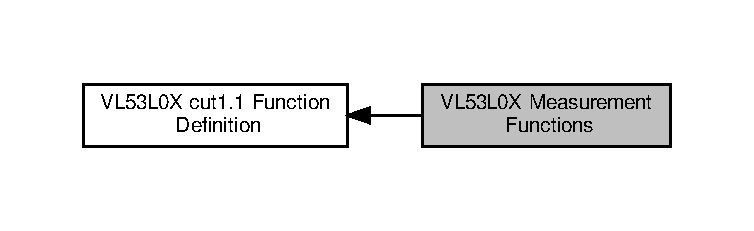
\includegraphics[width=350pt]{group__VL53L0X__measurement__group}
\end{center}
\end{figure}
\subsection*{Functions}
\begin{DoxyCompactItemize}
\item 
V\+L53\+L0\+X\+\_\+\+A\+PI V\+L53\+L0\+X\+\_\+\+Error \hyperlink{group__VL53L0X__measurement__group_gad56ed8d1403da5d203e2418a1f57fa81}{V\+L53\+L0\+X\+\_\+\+Perform\+Single\+Measurement} (\hyperlink{group__VL53L0X__platform__group_ga2d6405308b1dd524b462f1b8fb97d167}{V\+L53\+L0\+X\+\_\+\+D\+EV} Dev)
\begin{DoxyCompactList}\small\item\em Single shot measurement. \end{DoxyCompactList}\item 
V\+L53\+L0\+X\+\_\+\+A\+PI V\+L53\+L0\+X\+\_\+\+Error \hyperlink{group__VL53L0X__measurement__group_gafaf70e8668f8c650875a8f3a54366a20}{V\+L53\+L0\+X\+\_\+\+Perform\+Ref\+Calibration} (\hyperlink{group__VL53L0X__platform__group_ga2d6405308b1dd524b462f1b8fb97d167}{V\+L53\+L0\+X\+\_\+\+D\+EV} Dev, \hyperlink{vl53l0x__types_8h_aba7bc1797add20fe3efdf37ced1182c5}{uint8\+\_\+t} $\ast$p\+Vhv\+Settings, \hyperlink{vl53l0x__types_8h_aba7bc1797add20fe3efdf37ced1182c5}{uint8\+\_\+t} $\ast$p\+Phase\+Cal)
\begin{DoxyCompactList}\small\item\em Perform Reference Calibration. \end{DoxyCompactList}\item 
V\+L53\+L0\+X\+\_\+\+A\+PI V\+L53\+L0\+X\+\_\+\+Error \hyperlink{group__VL53L0X__measurement__group_ga13087ecf932d9d92ba24081b652c066b}{V\+L53\+L0\+X\+\_\+\+Perform\+X\+Talk\+Measurement} (\hyperlink{group__VL53L0X__platform__group_ga2d6405308b1dd524b462f1b8fb97d167}{V\+L53\+L0\+X\+\_\+\+D\+EV} Dev, \hyperlink{vl53l0x__types_8h_a435d1572bf3f880d55459d9805097f62}{uint32\+\_\+t} Timeout\+Ms, \hyperlink{vl53l0x__types_8h_afb910790161809fc76e1a274a6349384}{Fix\+Point1616\+\_\+t} $\ast$p\+Xtalk\+Per\+Spad, \hyperlink{vl53l0x__types_8h_aba7bc1797add20fe3efdf37ced1182c5}{uint8\+\_\+t} $\ast$p\+Ambient\+Too\+High)
\begin{DoxyCompactList}\small\item\em Perform X\+Talk Measurement. \end{DoxyCompactList}\item 
V\+L53\+L0\+X\+\_\+\+A\+PI V\+L53\+L0\+X\+\_\+\+Error \hyperlink{group__VL53L0X__measurement__group_ga5f0f4a2846a8ecf746aa25f738e6b442}{V\+L53\+L0\+X\+\_\+\+Perform\+X\+Talk\+Calibration} (\hyperlink{group__VL53L0X__platform__group_ga2d6405308b1dd524b462f1b8fb97d167}{V\+L53\+L0\+X\+\_\+\+D\+EV} Dev, \hyperlink{vl53l0x__types_8h_afb910790161809fc76e1a274a6349384}{Fix\+Point1616\+\_\+t} X\+Talk\+Cal\+Distance, \hyperlink{vl53l0x__types_8h_afb910790161809fc76e1a274a6349384}{Fix\+Point1616\+\_\+t} $\ast$p\+X\+Talk\+Compensation\+Rate\+Mega\+Cps)
\begin{DoxyCompactList}\small\item\em Perform X\+Talk Calibration. \end{DoxyCompactList}\item 
V\+L53\+L0\+X\+\_\+\+A\+PI V\+L53\+L0\+X\+\_\+\+Error \hyperlink{group__VL53L0X__measurement__group_gab33cdad2e9d45dd096b784b17013df3e}{V\+L53\+L0\+X\+\_\+\+Perform\+Offset\+Calibration} (\hyperlink{group__VL53L0X__platform__group_ga2d6405308b1dd524b462f1b8fb97d167}{V\+L53\+L0\+X\+\_\+\+D\+EV} Dev, \hyperlink{vl53l0x__types_8h_afb910790161809fc76e1a274a6349384}{Fix\+Point1616\+\_\+t} Cal\+Distance\+Milli\+Meter, \hyperlink{vl53l0x__types_8h_a32f2e37ee053cf2ce8ca28d1f74630e5}{int32\+\_\+t} $\ast$p\+Offset\+Micro\+Meter)
\begin{DoxyCompactList}\small\item\em Perform Offset Calibration. \end{DoxyCompactList}\item 
V\+L53\+L0\+X\+\_\+\+A\+PI V\+L53\+L0\+X\+\_\+\+Error \hyperlink{group__VL53L0X__measurement__group_gadd79559c9b3ef6ca4c4d378f08115be4}{V\+L53\+L0\+X\+\_\+\+Start\+Measurement} (\hyperlink{group__VL53L0X__platform__group_ga2d6405308b1dd524b462f1b8fb97d167}{V\+L53\+L0\+X\+\_\+\+D\+EV} Dev)
\begin{DoxyCompactList}\small\item\em Start device measurement. \end{DoxyCompactList}\item 
V\+L53\+L0\+X\+\_\+\+A\+PI V\+L53\+L0\+X\+\_\+\+Error \hyperlink{group__VL53L0X__measurement__group_ga7d2e62a19cd5dc5cd9a73b819e745888}{V\+L53\+L0\+X\+\_\+\+Stop\+Measurement} (\hyperlink{group__VL53L0X__platform__group_ga2d6405308b1dd524b462f1b8fb97d167}{V\+L53\+L0\+X\+\_\+\+D\+EV} Dev)
\begin{DoxyCompactList}\small\item\em Stop device measurement. \end{DoxyCompactList}\item 
V\+L53\+L0\+X\+\_\+\+A\+PI V\+L53\+L0\+X\+\_\+\+Error \hyperlink{group__VL53L0X__measurement__group_ga0052a146d166a0816ab696afda87ff49}{V\+L53\+L0\+X\+\_\+\+Get\+Measurement\+Data\+Ready} (\hyperlink{group__VL53L0X__platform__group_ga2d6405308b1dd524b462f1b8fb97d167}{V\+L53\+L0\+X\+\_\+\+D\+EV} Dev, \hyperlink{vl53l0x__types_8h_aba7bc1797add20fe3efdf37ced1182c5}{uint8\+\_\+t} $\ast$p\+Measurement\+Data\+Ready)
\begin{DoxyCompactList}\small\item\em Return Measurement Data Ready. \end{DoxyCompactList}\item 
V\+L53\+L0\+X\+\_\+\+A\+PI V\+L53\+L0\+X\+\_\+\+Error \hyperlink{group__VL53L0X__measurement__group_ga36e842f2f53c046d0f3a5e53f37113c3}{V\+L53\+L0\+X\+\_\+\+Wait\+Device\+Ready\+For\+New\+Measurement} (\hyperlink{group__VL53L0X__platform__group_ga2d6405308b1dd524b462f1b8fb97d167}{V\+L53\+L0\+X\+\_\+\+D\+EV} Dev, \hyperlink{vl53l0x__types_8h_a435d1572bf3f880d55459d9805097f62}{uint32\+\_\+t} Max\+Loop)
\begin{DoxyCompactList}\small\item\em Wait for device ready for a new measurement command. Blocking function. \end{DoxyCompactList}\item 
V\+L53\+L0\+X\+\_\+\+A\+PI V\+L53\+L0\+X\+\_\+\+Error \hyperlink{group__VL53L0X__measurement__group_ga744e1c15a276c1ecc68e308ac66ea414}{V\+L53\+L0\+X\+\_\+\+Get\+Measurement\+Ref\+Signal} (\hyperlink{group__VL53L0X__platform__group_ga2d6405308b1dd524b462f1b8fb97d167}{V\+L53\+L0\+X\+\_\+\+D\+EV} Dev, \hyperlink{vl53l0x__types_8h_afb910790161809fc76e1a274a6349384}{Fix\+Point1616\+\_\+t} $\ast$p\+Measurement\+Ref\+Signal)
\begin{DoxyCompactList}\small\item\em Retrieve the Reference Signal after a measurements. \end{DoxyCompactList}\item 
V\+L53\+L0\+X\+\_\+\+A\+PI V\+L53\+L0\+X\+\_\+\+Error \hyperlink{group__VL53L0X__measurement__group_ga2ed3769943964e7c24f3c8a06ef14ad7}{V\+L53\+L0\+X\+\_\+\+Get\+Ranging\+Measurement\+Data} (\hyperlink{group__VL53L0X__platform__group_ga2d6405308b1dd524b462f1b8fb97d167}{V\+L53\+L0\+X\+\_\+\+D\+EV} Dev, \hyperlink{structVL53L0X__RangingMeasurementData__t}{V\+L53\+L0\+X\+\_\+\+Ranging\+Measurement\+Data\+\_\+t} $\ast$p\+Ranging\+Measurement\+Data)
\begin{DoxyCompactList}\small\item\em Retrieve the measurements from device for a given setup. \end{DoxyCompactList}\item 
V\+L53\+L0\+X\+\_\+\+A\+PI V\+L53\+L0\+X\+\_\+\+Error \hyperlink{group__VL53L0X__measurement__group_ga774bd207d8451e932a524bd24c19e761}{V\+L53\+L0\+X\+\_\+\+Get\+Histogram\+Measurement\+Data} (\hyperlink{group__VL53L0X__platform__group_ga2d6405308b1dd524b462f1b8fb97d167}{V\+L53\+L0\+X\+\_\+\+D\+EV} Dev, \hyperlink{structVL53L0X__HistogramMeasurementData__t}{V\+L53\+L0\+X\+\_\+\+Histogram\+Measurement\+Data\+\_\+t} $\ast$p\+Histogram\+Measurement\+Data)
\begin{DoxyCompactList}\small\item\em Retrieve the measurements from device for a given setup. \end{DoxyCompactList}\item 
V\+L53\+L0\+X\+\_\+\+A\+PI V\+L53\+L0\+X\+\_\+\+Error \hyperlink{group__VL53L0X__measurement__group_gae81888494fb896a4a8922f16832291c1}{V\+L53\+L0\+X\+\_\+\+Perform\+Single\+Ranging\+Measurement} (\hyperlink{group__VL53L0X__platform__group_ga2d6405308b1dd524b462f1b8fb97d167}{V\+L53\+L0\+X\+\_\+\+D\+EV} Dev, \hyperlink{structVL53L0X__RangingMeasurementData__t}{V\+L53\+L0\+X\+\_\+\+Ranging\+Measurement\+Data\+\_\+t} $\ast$p\+Ranging\+Measurement\+Data)
\begin{DoxyCompactList}\small\item\em Performs a single ranging measurement and retrieve the ranging measurement data. \end{DoxyCompactList}\item 
V\+L53\+L0\+X\+\_\+\+A\+PI V\+L53\+L0\+X\+\_\+\+Error \hyperlink{group__VL53L0X__measurement__group_ga9607a687a23e621f2c7803374e34a5c5}{V\+L53\+L0\+X\+\_\+\+Perform\+Single\+Histogram\+Measurement} (\hyperlink{group__VL53L0X__platform__group_ga2d6405308b1dd524b462f1b8fb97d167}{V\+L53\+L0\+X\+\_\+\+D\+EV} Dev, \hyperlink{structVL53L0X__HistogramMeasurementData__t}{V\+L53\+L0\+X\+\_\+\+Histogram\+Measurement\+Data\+\_\+t} $\ast$p\+Histogram\+Measurement\+Data)
\begin{DoxyCompactList}\small\item\em Performs a single histogram measurement and retrieve the histogram measurement data Is equivalent to V\+L53\+L0\+X\+\_\+\+Perform\+Single\+Measurement + V\+L53\+L0\+X\+\_\+\+Get\+Histogram\+Measurement\+Data. \end{DoxyCompactList}\item 
V\+L53\+L0\+X\+\_\+\+A\+PI V\+L53\+L0\+X\+\_\+\+Error \hyperlink{group__VL53L0X__measurement__group_ga85c9be1dd8d1cb3b5ed70630e530b6d0}{V\+L53\+L0\+X\+\_\+\+Set\+Number\+Of\+R\+O\+I\+Zones} (\hyperlink{group__VL53L0X__platform__group_ga2d6405308b1dd524b462f1b8fb97d167}{V\+L53\+L0\+X\+\_\+\+D\+EV} Dev, \hyperlink{vl53l0x__types_8h_aba7bc1797add20fe3efdf37ced1182c5}{uint8\+\_\+t} Number\+Of\+R\+O\+I\+Zones)
\begin{DoxyCompactList}\small\item\em Set the number of R\+OI Zones to be used for a specific Device. \end{DoxyCompactList}\item 
V\+L53\+L0\+X\+\_\+\+A\+PI V\+L53\+L0\+X\+\_\+\+Error \hyperlink{group__VL53L0X__measurement__group_gad345958f05c6b130f35c569dd0d0e4f8}{V\+L53\+L0\+X\+\_\+\+Get\+Number\+Of\+R\+O\+I\+Zones} (\hyperlink{group__VL53L0X__platform__group_ga2d6405308b1dd524b462f1b8fb97d167}{V\+L53\+L0\+X\+\_\+\+D\+EV} Dev, \hyperlink{vl53l0x__types_8h_aba7bc1797add20fe3efdf37ced1182c5}{uint8\+\_\+t} $\ast$p\+Number\+Of\+R\+O\+I\+Zones)
\begin{DoxyCompactList}\small\item\em Get the number of R\+OI Zones managed by the Device. \end{DoxyCompactList}\item 
V\+L53\+L0\+X\+\_\+\+A\+PI V\+L53\+L0\+X\+\_\+\+Error \hyperlink{group__VL53L0X__measurement__group_gad3d40b6a62638f54f2a87289030e27e7}{V\+L53\+L0\+X\+\_\+\+Get\+Max\+Number\+Of\+R\+O\+I\+Zones} (\hyperlink{group__VL53L0X__platform__group_ga2d6405308b1dd524b462f1b8fb97d167}{V\+L53\+L0\+X\+\_\+\+D\+EV} Dev, \hyperlink{vl53l0x__types_8h_aba7bc1797add20fe3efdf37ced1182c5}{uint8\+\_\+t} $\ast$p\+Max\+Number\+Of\+R\+O\+I\+Zones)
\begin{DoxyCompactList}\small\item\em Get the Maximum number of R\+OI Zones managed by the Device. \end{DoxyCompactList}\end{DoxyCompactItemize}


\subsection{Detailed Description}
Functions used for the measurements. 



\subsection{Function Documentation}
\mbox{\Hypertarget{group__VL53L0X__measurement__group_ga774bd207d8451e932a524bd24c19e761}\label{group__VL53L0X__measurement__group_ga774bd207d8451e932a524bd24c19e761}} 
\index{V\+L53\+L0\+X Measurement Functions@{V\+L53\+L0\+X Measurement Functions}!V\+L53\+L0\+X\+\_\+\+Get\+Histogram\+Measurement\+Data@{V\+L53\+L0\+X\+\_\+\+Get\+Histogram\+Measurement\+Data}}
\index{V\+L53\+L0\+X\+\_\+\+Get\+Histogram\+Measurement\+Data@{V\+L53\+L0\+X\+\_\+\+Get\+Histogram\+Measurement\+Data}!V\+L53\+L0\+X Measurement Functions@{V\+L53\+L0\+X Measurement Functions}}
\subsubsection{\texorpdfstring{V\+L53\+L0\+X\+\_\+\+Get\+Histogram\+Measurement\+Data()}{VL53L0X\_GetHistogramMeasurementData()}}
{\footnotesize\ttfamily V\+L53\+L0\+X\+\_\+\+A\+PI V\+L53\+L0\+X\+\_\+\+Error V\+L53\+L0\+X\+\_\+\+Get\+Histogram\+Measurement\+Data (\begin{DoxyParamCaption}\item[{\hyperlink{group__VL53L0X__platform__group_ga2d6405308b1dd524b462f1b8fb97d167}{V\+L53\+L0\+X\+\_\+\+D\+EV}}]{Dev,  }\item[{\hyperlink{structVL53L0X__HistogramMeasurementData__t}{V\+L53\+L0\+X\+\_\+\+Histogram\+Measurement\+Data\+\_\+t} $\ast$}]{p\+Histogram\+Measurement\+Data }\end{DoxyParamCaption})}



Retrieve the measurements from device for a given setup. 

\begin{DoxyParagraph}{Function Description}
Get data from last successful Histogram measurement 
\end{DoxyParagraph}
\begin{DoxyWarning}{Warning}
U\+S\+ER should take care about {\itshape \hyperlink{group__VL53L0X__measurement__group_gad345958f05c6b130f35c569dd0d0e4f8}{V\+L53\+L0\+X\+\_\+\+Get\+Number\+Of\+R\+O\+I\+Zones()}} before get data. P\+AL will fill a Number\+Of\+R\+O\+I\+Zones times the corresponding data structure used in the measurement function.
\end{DoxyWarning}
\begin{DoxyNote}{Note}
This function is not Implemented
\end{DoxyNote}

\begin{DoxyParams}{Parameters}
{\em Dev} & Device Handle \\
\hline
{\em p\+Histogram\+Measurement\+Data} & Pointer to the histogram data structure. \\
\hline
\end{DoxyParams}
\begin{DoxyReturn}{Returns}
V\+L53\+L0\+X\+\_\+\+E\+R\+R\+O\+R\+\_\+\+N\+O\+T\+\_\+\+I\+M\+P\+L\+E\+M\+E\+N\+T\+ED Not implemented 
\end{DoxyReturn}
\mbox{\Hypertarget{group__VL53L0X__measurement__group_gad3d40b6a62638f54f2a87289030e27e7}\label{group__VL53L0X__measurement__group_gad3d40b6a62638f54f2a87289030e27e7}} 
\index{V\+L53\+L0\+X Measurement Functions@{V\+L53\+L0\+X Measurement Functions}!V\+L53\+L0\+X\+\_\+\+Get\+Max\+Number\+Of\+R\+O\+I\+Zones@{V\+L53\+L0\+X\+\_\+\+Get\+Max\+Number\+Of\+R\+O\+I\+Zones}}
\index{V\+L53\+L0\+X\+\_\+\+Get\+Max\+Number\+Of\+R\+O\+I\+Zones@{V\+L53\+L0\+X\+\_\+\+Get\+Max\+Number\+Of\+R\+O\+I\+Zones}!V\+L53\+L0\+X Measurement Functions@{V\+L53\+L0\+X Measurement Functions}}
\subsubsection{\texorpdfstring{V\+L53\+L0\+X\+\_\+\+Get\+Max\+Number\+Of\+R\+O\+I\+Zones()}{VL53L0X\_GetMaxNumberOfROIZones()}}
{\footnotesize\ttfamily V\+L53\+L0\+X\+\_\+\+A\+PI V\+L53\+L0\+X\+\_\+\+Error V\+L53\+L0\+X\+\_\+\+Get\+Max\+Number\+Of\+R\+O\+I\+Zones (\begin{DoxyParamCaption}\item[{\hyperlink{group__VL53L0X__platform__group_ga2d6405308b1dd524b462f1b8fb97d167}{V\+L53\+L0\+X\+\_\+\+D\+EV}}]{Dev,  }\item[{\hyperlink{vl53l0x__types_8h_aba7bc1797add20fe3efdf37ced1182c5}{uint8\+\_\+t} $\ast$}]{p\+Max\+Number\+Of\+R\+O\+I\+Zones }\end{DoxyParamCaption})}



Get the Maximum number of R\+OI Zones managed by the Device. 

\begin{DoxyParagraph}{Function Description}
Get Maximum number of R\+OI Zones managed by the Device.
\end{DoxyParagraph}
\begin{DoxyNote}{Note}
This function doesn\textquotesingle{}t Access to the device
\end{DoxyNote}

\begin{DoxyParams}{Parameters}
{\em Dev} & Device Handle \\
\hline
{\em p\+Max\+Number\+Of\+R\+O\+I\+Zones} & Pointer to the Maximum Number of R\+OI Zones value. \\
\hline
\end{DoxyParams}
\begin{DoxyReturn}{Returns}
V\+L53\+L0\+X\+\_\+\+E\+R\+R\+O\+R\+\_\+\+N\+O\+NE Success 
\end{DoxyReturn}
\mbox{\Hypertarget{group__VL53L0X__measurement__group_ga0052a146d166a0816ab696afda87ff49}\label{group__VL53L0X__measurement__group_ga0052a146d166a0816ab696afda87ff49}} 
\index{V\+L53\+L0\+X Measurement Functions@{V\+L53\+L0\+X Measurement Functions}!V\+L53\+L0\+X\+\_\+\+Get\+Measurement\+Data\+Ready@{V\+L53\+L0\+X\+\_\+\+Get\+Measurement\+Data\+Ready}}
\index{V\+L53\+L0\+X\+\_\+\+Get\+Measurement\+Data\+Ready@{V\+L53\+L0\+X\+\_\+\+Get\+Measurement\+Data\+Ready}!V\+L53\+L0\+X Measurement Functions@{V\+L53\+L0\+X Measurement Functions}}
\subsubsection{\texorpdfstring{V\+L53\+L0\+X\+\_\+\+Get\+Measurement\+Data\+Ready()}{VL53L0X\_GetMeasurementDataReady()}}
{\footnotesize\ttfamily V\+L53\+L0\+X\+\_\+\+A\+PI V\+L53\+L0\+X\+\_\+\+Error V\+L53\+L0\+X\+\_\+\+Get\+Measurement\+Data\+Ready (\begin{DoxyParamCaption}\item[{\hyperlink{group__VL53L0X__platform__group_ga2d6405308b1dd524b462f1b8fb97d167}{V\+L53\+L0\+X\+\_\+\+D\+EV}}]{Dev,  }\item[{\hyperlink{vl53l0x__types_8h_aba7bc1797add20fe3efdf37ced1182c5}{uint8\+\_\+t} $\ast$}]{p\+Measurement\+Data\+Ready }\end{DoxyParamCaption})}



Return Measurement Data Ready. 

\begin{DoxyParagraph}{Function Description}
This function indicate that a measurement data is ready. This function check if interrupt mode is used then check is done accordingly. If perform function clear the interrupt, this function will not work, like in case of {\itshape \hyperlink{group__VL53L0X__measurement__group_gae81888494fb896a4a8922f16832291c1}{V\+L53\+L0\+X\+\_\+\+Perform\+Single\+Ranging\+Measurement()}}. \hyperlink{structThe}{The} previous function is blocking function, V\+L53\+L0\+X\+\_\+\+Get\+Measurement\+Data\+Ready is used for non-\/blocking capture.
\end{DoxyParagraph}
\begin{DoxyNote}{Note}
This function Access to the device
\end{DoxyNote}

\begin{DoxyParams}{Parameters}
{\em Dev} & Device Handle \\
\hline
{\em p\+Measurement\+Data\+Ready} & Pointer to Measurement Data Ready. 0=data not ready, 1 = data ready \\
\hline
\end{DoxyParams}
\begin{DoxyReturn}{Returns}
V\+L53\+L0\+X\+\_\+\+E\+R\+R\+O\+R\+\_\+\+N\+O\+NE Success 

\char`\"{}\+Other error code\char`\"{} See \+::\+V\+L53\+L0\+X\+\_\+\+Error 
\end{DoxyReturn}
\mbox{\Hypertarget{group__VL53L0X__measurement__group_ga744e1c15a276c1ecc68e308ac66ea414}\label{group__VL53L0X__measurement__group_ga744e1c15a276c1ecc68e308ac66ea414}} 
\index{V\+L53\+L0\+X Measurement Functions@{V\+L53\+L0\+X Measurement Functions}!V\+L53\+L0\+X\+\_\+\+Get\+Measurement\+Ref\+Signal@{V\+L53\+L0\+X\+\_\+\+Get\+Measurement\+Ref\+Signal}}
\index{V\+L53\+L0\+X\+\_\+\+Get\+Measurement\+Ref\+Signal@{V\+L53\+L0\+X\+\_\+\+Get\+Measurement\+Ref\+Signal}!V\+L53\+L0\+X Measurement Functions@{V\+L53\+L0\+X Measurement Functions}}
\subsubsection{\texorpdfstring{V\+L53\+L0\+X\+\_\+\+Get\+Measurement\+Ref\+Signal()}{VL53L0X\_GetMeasurementRefSignal()}}
{\footnotesize\ttfamily V\+L53\+L0\+X\+\_\+\+A\+PI V\+L53\+L0\+X\+\_\+\+Error V\+L53\+L0\+X\+\_\+\+Get\+Measurement\+Ref\+Signal (\begin{DoxyParamCaption}\item[{\hyperlink{group__VL53L0X__platform__group_ga2d6405308b1dd524b462f1b8fb97d167}{V\+L53\+L0\+X\+\_\+\+D\+EV}}]{Dev,  }\item[{\hyperlink{vl53l0x__types_8h_afb910790161809fc76e1a274a6349384}{Fix\+Point1616\+\_\+t} $\ast$}]{p\+Measurement\+Ref\+Signal }\end{DoxyParamCaption})}



Retrieve the Reference Signal after a measurements. 

\begin{DoxyParagraph}{Function Description}
Get Reference Signal from last successful Ranging measurement This function return a valid value after that you call the {\itshape \hyperlink{group__VL53L0X__measurement__group_ga2ed3769943964e7c24f3c8a06ef14ad7}{V\+L53\+L0\+X\+\_\+\+Get\+Ranging\+Measurement\+Data()}}.
\end{DoxyParagraph}
\begin{DoxyNote}{Note}
This function Access to the device
\end{DoxyNote}

\begin{DoxyParams}{Parameters}
{\em Dev} & Device Handle \\
\hline
{\em p\+Measurement\+Ref\+Signal} & Pointer to the Ref Signal to fill up. \\
\hline
\end{DoxyParams}
\begin{DoxyReturn}{Returns}
V\+L53\+L0\+X\+\_\+\+E\+R\+R\+O\+R\+\_\+\+N\+O\+NE Success 

\char`\"{}\+Other error code\char`\"{} See \+::\+V\+L53\+L0\+X\+\_\+\+Error 
\end{DoxyReturn}
\mbox{\Hypertarget{group__VL53L0X__measurement__group_gad345958f05c6b130f35c569dd0d0e4f8}\label{group__VL53L0X__measurement__group_gad345958f05c6b130f35c569dd0d0e4f8}} 
\index{V\+L53\+L0\+X Measurement Functions@{V\+L53\+L0\+X Measurement Functions}!V\+L53\+L0\+X\+\_\+\+Get\+Number\+Of\+R\+O\+I\+Zones@{V\+L53\+L0\+X\+\_\+\+Get\+Number\+Of\+R\+O\+I\+Zones}}
\index{V\+L53\+L0\+X\+\_\+\+Get\+Number\+Of\+R\+O\+I\+Zones@{V\+L53\+L0\+X\+\_\+\+Get\+Number\+Of\+R\+O\+I\+Zones}!V\+L53\+L0\+X Measurement Functions@{V\+L53\+L0\+X Measurement Functions}}
\subsubsection{\texorpdfstring{V\+L53\+L0\+X\+\_\+\+Get\+Number\+Of\+R\+O\+I\+Zones()}{VL53L0X\_GetNumberOfROIZones()}}
{\footnotesize\ttfamily V\+L53\+L0\+X\+\_\+\+A\+PI V\+L53\+L0\+X\+\_\+\+Error V\+L53\+L0\+X\+\_\+\+Get\+Number\+Of\+R\+O\+I\+Zones (\begin{DoxyParamCaption}\item[{\hyperlink{group__VL53L0X__platform__group_ga2d6405308b1dd524b462f1b8fb97d167}{V\+L53\+L0\+X\+\_\+\+D\+EV}}]{Dev,  }\item[{\hyperlink{vl53l0x__types_8h_aba7bc1797add20fe3efdf37ced1182c5}{uint8\+\_\+t} $\ast$}]{p\+Number\+Of\+R\+O\+I\+Zones }\end{DoxyParamCaption})}



Get the number of R\+OI Zones managed by the Device. 

\begin{DoxyParagraph}{Function Description}
Get number of R\+OI Zones managed by the Device U\+S\+ER should take care about {\itshape \hyperlink{group__VL53L0X__measurement__group_gad345958f05c6b130f35c569dd0d0e4f8}{V\+L53\+L0\+X\+\_\+\+Get\+Number\+Of\+R\+O\+I\+Zones()}} before get data after a perform measurement. P\+AL will fill a Number\+Of\+R\+O\+I\+Zones times the corresponding data structure used in the measurement function.
\end{DoxyParagraph}
\begin{DoxyNote}{Note}
This function doesn\textquotesingle{}t Access to the device
\end{DoxyNote}

\begin{DoxyParams}{Parameters}
{\em Dev} & Device Handle \\
\hline
{\em p\+Number\+Of\+R\+O\+I\+Zones} & Pointer to the Number of R\+OI Zones value. \\
\hline
\end{DoxyParams}
\begin{DoxyReturn}{Returns}
V\+L53\+L0\+X\+\_\+\+E\+R\+R\+O\+R\+\_\+\+N\+O\+NE Success 
\end{DoxyReturn}
\mbox{\Hypertarget{group__VL53L0X__measurement__group_ga2ed3769943964e7c24f3c8a06ef14ad7}\label{group__VL53L0X__measurement__group_ga2ed3769943964e7c24f3c8a06ef14ad7}} 
\index{V\+L53\+L0\+X Measurement Functions@{V\+L53\+L0\+X Measurement Functions}!V\+L53\+L0\+X\+\_\+\+Get\+Ranging\+Measurement\+Data@{V\+L53\+L0\+X\+\_\+\+Get\+Ranging\+Measurement\+Data}}
\index{V\+L53\+L0\+X\+\_\+\+Get\+Ranging\+Measurement\+Data@{V\+L53\+L0\+X\+\_\+\+Get\+Ranging\+Measurement\+Data}!V\+L53\+L0\+X Measurement Functions@{V\+L53\+L0\+X Measurement Functions}}
\subsubsection{\texorpdfstring{V\+L53\+L0\+X\+\_\+\+Get\+Ranging\+Measurement\+Data()}{VL53L0X\_GetRangingMeasurementData()}}
{\footnotesize\ttfamily V\+L53\+L0\+X\+\_\+\+A\+PI V\+L53\+L0\+X\+\_\+\+Error V\+L53\+L0\+X\+\_\+\+Get\+Ranging\+Measurement\+Data (\begin{DoxyParamCaption}\item[{\hyperlink{group__VL53L0X__platform__group_ga2d6405308b1dd524b462f1b8fb97d167}{V\+L53\+L0\+X\+\_\+\+D\+EV}}]{Dev,  }\item[{\hyperlink{structVL53L0X__RangingMeasurementData__t}{V\+L53\+L0\+X\+\_\+\+Ranging\+Measurement\+Data\+\_\+t} $\ast$}]{p\+Ranging\+Measurement\+Data }\end{DoxyParamCaption})}



Retrieve the measurements from device for a given setup. 

\begin{DoxyParagraph}{Function Description}
Get data from last successful Ranging measurement 
\end{DoxyParagraph}
\begin{DoxyWarning}{Warning}
U\+S\+ER should take care about {\itshape \hyperlink{group__VL53L0X__measurement__group_gad345958f05c6b130f35c569dd0d0e4f8}{V\+L53\+L0\+X\+\_\+\+Get\+Number\+Of\+R\+O\+I\+Zones()}} before get data. P\+AL will fill a Number\+Of\+R\+O\+I\+Zones times the corresponding data structure used in the measurement function.
\end{DoxyWarning}
\begin{DoxyNote}{Note}
This function Access to the device
\end{DoxyNote}

\begin{DoxyParams}{Parameters}
{\em Dev} & Device Handle \\
\hline
{\em p\+Ranging\+Measurement\+Data} & Pointer to the data structure to fill up. \\
\hline
\end{DoxyParams}
\begin{DoxyReturn}{Returns}
V\+L53\+L0\+X\+\_\+\+E\+R\+R\+O\+R\+\_\+\+N\+O\+NE Success 

\char`\"{}\+Other error code\char`\"{} See \+::\+V\+L53\+L0\+X\+\_\+\+Error 
\end{DoxyReturn}
\mbox{\Hypertarget{group__VL53L0X__measurement__group_gab33cdad2e9d45dd096b784b17013df3e}\label{group__VL53L0X__measurement__group_gab33cdad2e9d45dd096b784b17013df3e}} 
\index{V\+L53\+L0\+X Measurement Functions@{V\+L53\+L0\+X Measurement Functions}!V\+L53\+L0\+X\+\_\+\+Perform\+Offset\+Calibration@{V\+L53\+L0\+X\+\_\+\+Perform\+Offset\+Calibration}}
\index{V\+L53\+L0\+X\+\_\+\+Perform\+Offset\+Calibration@{V\+L53\+L0\+X\+\_\+\+Perform\+Offset\+Calibration}!V\+L53\+L0\+X Measurement Functions@{V\+L53\+L0\+X Measurement Functions}}
\subsubsection{\texorpdfstring{V\+L53\+L0\+X\+\_\+\+Perform\+Offset\+Calibration()}{VL53L0X\_PerformOffsetCalibration()}}
{\footnotesize\ttfamily V\+L53\+L0\+X\+\_\+\+A\+PI V\+L53\+L0\+X\+\_\+\+Error V\+L53\+L0\+X\+\_\+\+Perform\+Offset\+Calibration (\begin{DoxyParamCaption}\item[{\hyperlink{group__VL53L0X__platform__group_ga2d6405308b1dd524b462f1b8fb97d167}{V\+L53\+L0\+X\+\_\+\+D\+EV}}]{Dev,  }\item[{\hyperlink{vl53l0x__types_8h_afb910790161809fc76e1a274a6349384}{Fix\+Point1616\+\_\+t}}]{Cal\+Distance\+Milli\+Meter,  }\item[{\hyperlink{vl53l0x__types_8h_a32f2e37ee053cf2ce8ca28d1f74630e5}{int32\+\_\+t} $\ast$}]{p\+Offset\+Micro\+Meter }\end{DoxyParamCaption})}



Perform Offset Calibration. 

Perform a Offset calibration of the Device. This function will launch a ranging measurement, if interrupts are enabled an interrupt will be done. This function will clear the interrupt generated automatically. This function will program a new value for the Offset calibration value This function will disable the V\+L53\+L0\+X\+\_\+\+C\+H\+E\+C\+K\+E\+N\+A\+B\+L\+E\+\_\+\+R\+A\+N\+G\+E\+\_\+\+I\+G\+N\+O\+R\+E\+\_\+\+T\+H\+R\+E\+S\+H\+O\+LD.

\begin{DoxyWarning}{Warning}
This function is a blocking function
\end{DoxyWarning}
\begin{DoxyNote}{Note}
This function Access to the device

This function does not change the device mode.
\end{DoxyNote}

\begin{DoxyParams}{Parameters}
{\em Dev} & Device Handle \\
\hline
{\em Cal\+Distance\+Milli\+Meter} & Calibration distance value used for the offset compensation. \\
\hline
{\em p\+Offset\+Micro\+Meter} & Pointer to new Offset value computed by the function.\\
\hline
\end{DoxyParams}
\begin{DoxyReturn}{Returns}
V\+L53\+L0\+X\+\_\+\+E\+R\+R\+O\+R\+\_\+\+N\+O\+NE Success 

\char`\"{}\+Other error code\char`\"{} See \+::\+V\+L53\+L0\+X\+\_\+\+Error 
\end{DoxyReturn}
\mbox{\Hypertarget{group__VL53L0X__measurement__group_gafaf70e8668f8c650875a8f3a54366a20}\label{group__VL53L0X__measurement__group_gafaf70e8668f8c650875a8f3a54366a20}} 
\index{V\+L53\+L0\+X Measurement Functions@{V\+L53\+L0\+X Measurement Functions}!V\+L53\+L0\+X\+\_\+\+Perform\+Ref\+Calibration@{V\+L53\+L0\+X\+\_\+\+Perform\+Ref\+Calibration}}
\index{V\+L53\+L0\+X\+\_\+\+Perform\+Ref\+Calibration@{V\+L53\+L0\+X\+\_\+\+Perform\+Ref\+Calibration}!V\+L53\+L0\+X Measurement Functions@{V\+L53\+L0\+X Measurement Functions}}
\subsubsection{\texorpdfstring{V\+L53\+L0\+X\+\_\+\+Perform\+Ref\+Calibration()}{VL53L0X\_PerformRefCalibration()}}
{\footnotesize\ttfamily V\+L53\+L0\+X\+\_\+\+A\+PI V\+L53\+L0\+X\+\_\+\+Error V\+L53\+L0\+X\+\_\+\+Perform\+Ref\+Calibration (\begin{DoxyParamCaption}\item[{\hyperlink{group__VL53L0X__platform__group_ga2d6405308b1dd524b462f1b8fb97d167}{V\+L53\+L0\+X\+\_\+\+D\+EV}}]{Dev,  }\item[{\hyperlink{vl53l0x__types_8h_aba7bc1797add20fe3efdf37ced1182c5}{uint8\+\_\+t} $\ast$}]{p\+Vhv\+Settings,  }\item[{\hyperlink{vl53l0x__types_8h_aba7bc1797add20fe3efdf37ced1182c5}{uint8\+\_\+t} $\ast$}]{p\+Phase\+Cal }\end{DoxyParamCaption})}



Perform Reference Calibration. 

Perform a reference calibration of the Device. This function should be run from time to time before doing a ranging measurement. This function will launch a special ranging measurement, so if interrupt are enable an interrupt will be done. This function will clear the interrupt generated automatically.

\begin{DoxyWarning}{Warning}
This function is a blocking function
\end{DoxyWarning}
\begin{DoxyNote}{Note}
This function Access to the device
\end{DoxyNote}

\begin{DoxyParams}{Parameters}
{\em Dev} & Device Handle \\
\hline
{\em p\+Vhv\+Settings} & Pointer to vhv settings parameter. \\
\hline
{\em p\+Phase\+Cal} & Pointer to Phase\+Cal parameter. \\
\hline
\end{DoxyParams}
\begin{DoxyReturn}{Returns}
V\+L53\+L0\+X\+\_\+\+E\+R\+R\+O\+R\+\_\+\+N\+O\+NE Success 

\char`\"{}\+Other error code\char`\"{} See \+::\+V\+L53\+L0\+X\+\_\+\+Error 
\end{DoxyReturn}
\mbox{\Hypertarget{group__VL53L0X__measurement__group_ga9607a687a23e621f2c7803374e34a5c5}\label{group__VL53L0X__measurement__group_ga9607a687a23e621f2c7803374e34a5c5}} 
\index{V\+L53\+L0\+X Measurement Functions@{V\+L53\+L0\+X Measurement Functions}!V\+L53\+L0\+X\+\_\+\+Perform\+Single\+Histogram\+Measurement@{V\+L53\+L0\+X\+\_\+\+Perform\+Single\+Histogram\+Measurement}}
\index{V\+L53\+L0\+X\+\_\+\+Perform\+Single\+Histogram\+Measurement@{V\+L53\+L0\+X\+\_\+\+Perform\+Single\+Histogram\+Measurement}!V\+L53\+L0\+X Measurement Functions@{V\+L53\+L0\+X Measurement Functions}}
\subsubsection{\texorpdfstring{V\+L53\+L0\+X\+\_\+\+Perform\+Single\+Histogram\+Measurement()}{VL53L0X\_PerformSingleHistogramMeasurement()}}
{\footnotesize\ttfamily V\+L53\+L0\+X\+\_\+\+A\+PI V\+L53\+L0\+X\+\_\+\+Error V\+L53\+L0\+X\+\_\+\+Perform\+Single\+Histogram\+Measurement (\begin{DoxyParamCaption}\item[{\hyperlink{group__VL53L0X__platform__group_ga2d6405308b1dd524b462f1b8fb97d167}{V\+L53\+L0\+X\+\_\+\+D\+EV}}]{Dev,  }\item[{\hyperlink{structVL53L0X__HistogramMeasurementData__t}{V\+L53\+L0\+X\+\_\+\+Histogram\+Measurement\+Data\+\_\+t} $\ast$}]{p\+Histogram\+Measurement\+Data }\end{DoxyParamCaption})}



Performs a single histogram measurement and retrieve the histogram measurement data Is equivalent to V\+L53\+L0\+X\+\_\+\+Perform\+Single\+Measurement + V\+L53\+L0\+X\+\_\+\+Get\+Histogram\+Measurement\+Data. 

\begin{DoxyParagraph}{Function Description}
Get data from last successful Ranging measurement. This function will clear the interrupt in case of these are enabled.
\end{DoxyParagraph}
\begin{DoxyNote}{Note}
This function is not Implemented
\end{DoxyNote}

\begin{DoxyParams}{Parameters}
{\em Dev} & Device Handle \\
\hline
{\em p\+Histogram\+Measurement\+Data} & Pointer to the data structure to fill up. \\
\hline
\end{DoxyParams}
\begin{DoxyReturn}{Returns}
V\+L53\+L0\+X\+\_\+\+E\+R\+R\+O\+R\+\_\+\+N\+O\+T\+\_\+\+I\+M\+P\+L\+E\+M\+E\+N\+T\+ED Not implemented 
\end{DoxyReturn}
\mbox{\Hypertarget{group__VL53L0X__measurement__group_gad56ed8d1403da5d203e2418a1f57fa81}\label{group__VL53L0X__measurement__group_gad56ed8d1403da5d203e2418a1f57fa81}} 
\index{V\+L53\+L0\+X Measurement Functions@{V\+L53\+L0\+X Measurement Functions}!V\+L53\+L0\+X\+\_\+\+Perform\+Single\+Measurement@{V\+L53\+L0\+X\+\_\+\+Perform\+Single\+Measurement}}
\index{V\+L53\+L0\+X\+\_\+\+Perform\+Single\+Measurement@{V\+L53\+L0\+X\+\_\+\+Perform\+Single\+Measurement}!V\+L53\+L0\+X Measurement Functions@{V\+L53\+L0\+X Measurement Functions}}
\subsubsection{\texorpdfstring{V\+L53\+L0\+X\+\_\+\+Perform\+Single\+Measurement()}{VL53L0X\_PerformSingleMeasurement()}}
{\footnotesize\ttfamily V\+L53\+L0\+X\+\_\+\+A\+PI V\+L53\+L0\+X\+\_\+\+Error V\+L53\+L0\+X\+\_\+\+Perform\+Single\+Measurement (\begin{DoxyParamCaption}\item[{\hyperlink{group__VL53L0X__platform__group_ga2d6405308b1dd524b462f1b8fb97d167}{V\+L53\+L0\+X\+\_\+\+D\+EV}}]{Dev }\end{DoxyParamCaption})}



Single shot measurement. 

\begin{DoxyParagraph}{Function Description}
Perform simple measurement sequence (Start measure, Wait measure to end, and returns when measurement is done). Once function returns, user can get valid data by calling V\+L53\+L0\+X\+\_\+\+Get\+Ranging\+Measurement or V\+L53\+L0\+X\+\_\+\+Get\+Histogram\+Measurement depending on defined measurement mode User should Clear the interrupt in case this are enabled by using the function \hyperlink{group__VL53L0X__interrupt__group_gaa84b2cf5cd87b118b9a43e7ae764447e}{V\+L53\+L0\+X\+\_\+\+Clear\+Interrupt\+Mask()}.
\end{DoxyParagraph}
\begin{DoxyWarning}{Warning}
This function is a blocking function
\end{DoxyWarning}
\begin{DoxyNote}{Note}
This function Access to the device
\end{DoxyNote}

\begin{DoxyParams}{Parameters}
{\em Dev} & Device Handle \\
\hline
\end{DoxyParams}
\begin{DoxyReturn}{Returns}
V\+L53\+L0\+X\+\_\+\+E\+R\+R\+O\+R\+\_\+\+N\+O\+NE Success 

\char`\"{}\+Other error code\char`\"{} See \+::\+V\+L53\+L0\+X\+\_\+\+Error 
\end{DoxyReturn}
\mbox{\Hypertarget{group__VL53L0X__measurement__group_gae81888494fb896a4a8922f16832291c1}\label{group__VL53L0X__measurement__group_gae81888494fb896a4a8922f16832291c1}} 
\index{V\+L53\+L0\+X Measurement Functions@{V\+L53\+L0\+X Measurement Functions}!V\+L53\+L0\+X\+\_\+\+Perform\+Single\+Ranging\+Measurement@{V\+L53\+L0\+X\+\_\+\+Perform\+Single\+Ranging\+Measurement}}
\index{V\+L53\+L0\+X\+\_\+\+Perform\+Single\+Ranging\+Measurement@{V\+L53\+L0\+X\+\_\+\+Perform\+Single\+Ranging\+Measurement}!V\+L53\+L0\+X Measurement Functions@{V\+L53\+L0\+X Measurement Functions}}
\subsubsection{\texorpdfstring{V\+L53\+L0\+X\+\_\+\+Perform\+Single\+Ranging\+Measurement()}{VL53L0X\_PerformSingleRangingMeasurement()}}
{\footnotesize\ttfamily V\+L53\+L0\+X\+\_\+\+A\+PI V\+L53\+L0\+X\+\_\+\+Error V\+L53\+L0\+X\+\_\+\+Perform\+Single\+Ranging\+Measurement (\begin{DoxyParamCaption}\item[{\hyperlink{group__VL53L0X__platform__group_ga2d6405308b1dd524b462f1b8fb97d167}{V\+L53\+L0\+X\+\_\+\+D\+EV}}]{Dev,  }\item[{\hyperlink{structVL53L0X__RangingMeasurementData__t}{V\+L53\+L0\+X\+\_\+\+Ranging\+Measurement\+Data\+\_\+t} $\ast$}]{p\+Ranging\+Measurement\+Data }\end{DoxyParamCaption})}



Performs a single ranging measurement and retrieve the ranging measurement data. 

\begin{DoxyParagraph}{Function Description}
This function will change the device mode to V\+L53\+L0\+X\+\_\+\+D\+E\+V\+I\+C\+E\+M\+O\+D\+E\+\_\+\+S\+I\+N\+G\+L\+E\+\_\+\+R\+A\+N\+G\+I\+NG with {\itshape \hyperlink{group__VL53L0X__parameters__group_ga547bf7479b5ec799db4aafb7111271f7}{V\+L53\+L0\+X\+\_\+\+Set\+Device\+Mode()}}, It performs measurement with {\itshape \hyperlink{group__VL53L0X__measurement__group_gad56ed8d1403da5d203e2418a1f57fa81}{V\+L53\+L0\+X\+\_\+\+Perform\+Single\+Measurement()}} It get data from last successful Ranging measurement with {\itshape V\+L53\+L0\+X\+\_\+\+Get\+Ranging\+Measurement\+Data}. Finally it clear the interrupt with {\itshape \hyperlink{group__VL53L0X__interrupt__group_gaa84b2cf5cd87b118b9a43e7ae764447e}{V\+L53\+L0\+X\+\_\+\+Clear\+Interrupt\+Mask()}}.
\end{DoxyParagraph}
\begin{DoxyNote}{Note}
This function Access to the device

This function change the device mode to V\+L53\+L0\+X\+\_\+\+D\+E\+V\+I\+C\+E\+M\+O\+D\+E\+\_\+\+S\+I\+N\+G\+L\+E\+\_\+\+R\+A\+N\+G\+I\+NG
\end{DoxyNote}

\begin{DoxyParams}{Parameters}
{\em Dev} & Device Handle \\
\hline
{\em p\+Ranging\+Measurement\+Data} & Pointer to the data structure to fill up. \\
\hline
\end{DoxyParams}
\begin{DoxyReturn}{Returns}
V\+L53\+L0\+X\+\_\+\+E\+R\+R\+O\+R\+\_\+\+N\+O\+NE Success 

\char`\"{}\+Other error code\char`\"{} See \+::\+V\+L53\+L0\+X\+\_\+\+Error 
\end{DoxyReturn}
\mbox{\Hypertarget{group__VL53L0X__measurement__group_ga5f0f4a2846a8ecf746aa25f738e6b442}\label{group__VL53L0X__measurement__group_ga5f0f4a2846a8ecf746aa25f738e6b442}} 
\index{V\+L53\+L0\+X Measurement Functions@{V\+L53\+L0\+X Measurement Functions}!V\+L53\+L0\+X\+\_\+\+Perform\+X\+Talk\+Calibration@{V\+L53\+L0\+X\+\_\+\+Perform\+X\+Talk\+Calibration}}
\index{V\+L53\+L0\+X\+\_\+\+Perform\+X\+Talk\+Calibration@{V\+L53\+L0\+X\+\_\+\+Perform\+X\+Talk\+Calibration}!V\+L53\+L0\+X Measurement Functions@{V\+L53\+L0\+X Measurement Functions}}
\subsubsection{\texorpdfstring{V\+L53\+L0\+X\+\_\+\+Perform\+X\+Talk\+Calibration()}{VL53L0X\_PerformXTalkCalibration()}}
{\footnotesize\ttfamily V\+L53\+L0\+X\+\_\+\+A\+PI V\+L53\+L0\+X\+\_\+\+Error V\+L53\+L0\+X\+\_\+\+Perform\+X\+Talk\+Calibration (\begin{DoxyParamCaption}\item[{\hyperlink{group__VL53L0X__platform__group_ga2d6405308b1dd524b462f1b8fb97d167}{V\+L53\+L0\+X\+\_\+\+D\+EV}}]{Dev,  }\item[{\hyperlink{vl53l0x__types_8h_afb910790161809fc76e1a274a6349384}{Fix\+Point1616\+\_\+t}}]{X\+Talk\+Cal\+Distance,  }\item[{\hyperlink{vl53l0x__types_8h_afb910790161809fc76e1a274a6349384}{Fix\+Point1616\+\_\+t} $\ast$}]{p\+X\+Talk\+Compensation\+Rate\+Mega\+Cps }\end{DoxyParamCaption})}



Perform X\+Talk Calibration. 

Perform a X\+Talk calibration of the Device. This function will launch a ranging measurement, if interrupts are enabled an interrupt will be done. This function will clear the interrupt generated automatically. This function will program a new value for the X\+Talk compensation and it will enable the cross talk before exit. This function will disable the V\+L53\+L0\+X\+\_\+\+C\+H\+E\+C\+K\+E\+N\+A\+B\+L\+E\+\_\+\+R\+A\+N\+G\+E\+\_\+\+I\+G\+N\+O\+R\+E\+\_\+\+T\+H\+R\+E\+S\+H\+O\+LD.

\begin{DoxyWarning}{Warning}
This function is a blocking function
\end{DoxyWarning}
\begin{DoxyNote}{Note}
This function Access to the device

This function change the device mode to V\+L53\+L0\+X\+\_\+\+D\+E\+V\+I\+C\+E\+M\+O\+D\+E\+\_\+\+S\+I\+N\+G\+L\+E\+\_\+\+R\+A\+N\+G\+I\+NG
\end{DoxyNote}

\begin{DoxyParams}{Parameters}
{\em Dev} & Device Handle \\
\hline
{\em X\+Talk\+Cal\+Distance} & X\+Talk\+Cal\+Distance value used for the X\+Talk computation. \\
\hline
{\em p\+X\+Talk\+Compensation\+Rate\+Mega\+Cps} & Pointer to new X\+Talk\+Compensation value. \\
\hline
\end{DoxyParams}
\begin{DoxyReturn}{Returns}
V\+L53\+L0\+X\+\_\+\+E\+R\+R\+O\+R\+\_\+\+N\+O\+NE Success 

\char`\"{}\+Other error code\char`\"{} See \+::\+V\+L53\+L0\+X\+\_\+\+Error 
\end{DoxyReturn}
\mbox{\Hypertarget{group__VL53L0X__measurement__group_ga13087ecf932d9d92ba24081b652c066b}\label{group__VL53L0X__measurement__group_ga13087ecf932d9d92ba24081b652c066b}} 
\index{V\+L53\+L0\+X Measurement Functions@{V\+L53\+L0\+X Measurement Functions}!V\+L53\+L0\+X\+\_\+\+Perform\+X\+Talk\+Measurement@{V\+L53\+L0\+X\+\_\+\+Perform\+X\+Talk\+Measurement}}
\index{V\+L53\+L0\+X\+\_\+\+Perform\+X\+Talk\+Measurement@{V\+L53\+L0\+X\+\_\+\+Perform\+X\+Talk\+Measurement}!V\+L53\+L0\+X Measurement Functions@{V\+L53\+L0\+X Measurement Functions}}
\subsubsection{\texorpdfstring{V\+L53\+L0\+X\+\_\+\+Perform\+X\+Talk\+Measurement()}{VL53L0X\_PerformXTalkMeasurement()}}
{\footnotesize\ttfamily V\+L53\+L0\+X\+\_\+\+A\+PI V\+L53\+L0\+X\+\_\+\+Error V\+L53\+L0\+X\+\_\+\+Perform\+X\+Talk\+Measurement (\begin{DoxyParamCaption}\item[{\hyperlink{group__VL53L0X__platform__group_ga2d6405308b1dd524b462f1b8fb97d167}{V\+L53\+L0\+X\+\_\+\+D\+EV}}]{Dev,  }\item[{\hyperlink{vl53l0x__types_8h_a435d1572bf3f880d55459d9805097f62}{uint32\+\_\+t}}]{Timeout\+Ms,  }\item[{\hyperlink{vl53l0x__types_8h_afb910790161809fc76e1a274a6349384}{Fix\+Point1616\+\_\+t} $\ast$}]{p\+Xtalk\+Per\+Spad,  }\item[{\hyperlink{vl53l0x__types_8h_aba7bc1797add20fe3efdf37ced1182c5}{uint8\+\_\+t} $\ast$}]{p\+Ambient\+Too\+High }\end{DoxyParamCaption})}



Perform X\+Talk Measurement. 

Measures the current cross talk from glass in front of the sensor. This functions performs a histogram measurement and uses the results to measure the crosstalk. For the function to be successful, there must be no target in front of the sensor.

\begin{DoxyWarning}{Warning}
This function is a blocking function

This function is not supported when the final range vcsel clock period is set below 10 P\+C\+L\+KS.
\end{DoxyWarning}
\begin{DoxyNote}{Note}
This function Access to the device
\end{DoxyNote}

\begin{DoxyParams}{Parameters}
{\em Dev} & Device Handle \\
\hline
{\em Timeout\+Ms} & Histogram measurement duration. \\
\hline
{\em p\+Xtalk\+Per\+Spad} & Output parameter containing the crosstalk measurement result, in M\+C\+P\+S/\+Spad. Format fixpoint 16\+:16. \\
\hline
{\em p\+Ambient\+Too\+High} & Output parameter which indicate that p\+Xtalk\+Per\+Spad is not good if the Ambient is too high. \\
\hline
\end{DoxyParams}
\begin{DoxyReturn}{Returns}
V\+L53\+L0\+X\+\_\+\+E\+R\+R\+O\+R\+\_\+\+N\+O\+NE Success 

V\+L53\+L0\+X\+\_\+\+E\+R\+R\+O\+R\+\_\+\+I\+N\+V\+A\+L\+I\+D\+\_\+\+P\+A\+R\+A\+MS vcsel clock period not supported for this operation. Must not be less than 10\+P\+C\+L\+KS. 

\char`\"{}\+Other error code\char`\"{} See \+::\+V\+L53\+L0\+X\+\_\+\+Error 
\end{DoxyReturn}
\mbox{\Hypertarget{group__VL53L0X__measurement__group_ga85c9be1dd8d1cb3b5ed70630e530b6d0}\label{group__VL53L0X__measurement__group_ga85c9be1dd8d1cb3b5ed70630e530b6d0}} 
\index{V\+L53\+L0\+X Measurement Functions@{V\+L53\+L0\+X Measurement Functions}!V\+L53\+L0\+X\+\_\+\+Set\+Number\+Of\+R\+O\+I\+Zones@{V\+L53\+L0\+X\+\_\+\+Set\+Number\+Of\+R\+O\+I\+Zones}}
\index{V\+L53\+L0\+X\+\_\+\+Set\+Number\+Of\+R\+O\+I\+Zones@{V\+L53\+L0\+X\+\_\+\+Set\+Number\+Of\+R\+O\+I\+Zones}!V\+L53\+L0\+X Measurement Functions@{V\+L53\+L0\+X Measurement Functions}}
\subsubsection{\texorpdfstring{V\+L53\+L0\+X\+\_\+\+Set\+Number\+Of\+R\+O\+I\+Zones()}{VL53L0X\_SetNumberOfROIZones()}}
{\footnotesize\ttfamily V\+L53\+L0\+X\+\_\+\+A\+PI V\+L53\+L0\+X\+\_\+\+Error V\+L53\+L0\+X\+\_\+\+Set\+Number\+Of\+R\+O\+I\+Zones (\begin{DoxyParamCaption}\item[{\hyperlink{group__VL53L0X__platform__group_ga2d6405308b1dd524b462f1b8fb97d167}{V\+L53\+L0\+X\+\_\+\+D\+EV}}]{Dev,  }\item[{\hyperlink{vl53l0x__types_8h_aba7bc1797add20fe3efdf37ced1182c5}{uint8\+\_\+t}}]{Number\+Of\+R\+O\+I\+Zones }\end{DoxyParamCaption})}



Set the number of R\+OI Zones to be used for a specific Device. 

\begin{DoxyParagraph}{Function Description}
Set the number of R\+OI Zones to be used for a specific Device. \hyperlink{structThe}{The} programmed value should be less than the max number of R\+OI Zones given with {\itshape \hyperlink{group__VL53L0X__measurement__group_gad3d40b6a62638f54f2a87289030e27e7}{V\+L53\+L0\+X\+\_\+\+Get\+Max\+Number\+Of\+R\+O\+I\+Zones()}}. This version of A\+PI manage only one zone.
\end{DoxyParagraph}

\begin{DoxyParams}{Parameters}
{\em Dev} & Device Handle \\
\hline
{\em Number\+Of\+R\+O\+I\+Zones} & Number of R\+OI Zones to be used for a specific Device. \\
\hline
\end{DoxyParams}
\begin{DoxyReturn}{Returns}
V\+L53\+L0\+X\+\_\+\+E\+R\+R\+O\+R\+\_\+\+N\+O\+NE Success 

V\+L53\+L0\+X\+\_\+\+E\+R\+R\+O\+R\+\_\+\+I\+N\+V\+A\+L\+I\+D\+\_\+\+P\+A\+R\+A\+MS This error is returned if Number\+Of\+R\+O\+I\+Zones != 1 
\end{DoxyReturn}
\mbox{\Hypertarget{group__VL53L0X__measurement__group_gadd79559c9b3ef6ca4c4d378f08115be4}\label{group__VL53L0X__measurement__group_gadd79559c9b3ef6ca4c4d378f08115be4}} 
\index{V\+L53\+L0\+X Measurement Functions@{V\+L53\+L0\+X Measurement Functions}!V\+L53\+L0\+X\+\_\+\+Start\+Measurement@{V\+L53\+L0\+X\+\_\+\+Start\+Measurement}}
\index{V\+L53\+L0\+X\+\_\+\+Start\+Measurement@{V\+L53\+L0\+X\+\_\+\+Start\+Measurement}!V\+L53\+L0\+X Measurement Functions@{V\+L53\+L0\+X Measurement Functions}}
\subsubsection{\texorpdfstring{V\+L53\+L0\+X\+\_\+\+Start\+Measurement()}{VL53L0X\_StartMeasurement()}}
{\footnotesize\ttfamily V\+L53\+L0\+X\+\_\+\+A\+PI V\+L53\+L0\+X\+\_\+\+Error V\+L53\+L0\+X\+\_\+\+Start\+Measurement (\begin{DoxyParamCaption}\item[{\hyperlink{group__VL53L0X__platform__group_ga2d6405308b1dd524b462f1b8fb97d167}{V\+L53\+L0\+X\+\_\+\+D\+EV}}]{Dev }\end{DoxyParamCaption})}



Start device measurement. 

Started measurement will depend on device parameters set through {\itshape V\+L53\+L0\+X\+\_\+\+Set\+Parameters()} This is a non-\/blocking function. This function will change the V\+L53\+L0\+X\+\_\+\+State from V\+L53\+L0\+X\+\_\+\+S\+T\+A\+T\+E\+\_\+\+I\+D\+LE to V\+L53\+L0\+X\+\_\+\+S\+T\+A\+T\+E\+\_\+\+R\+U\+N\+N\+I\+NG.

\begin{DoxyNote}{Note}
This function Access to the device
\end{DoxyNote}

\begin{DoxyParams}{Parameters}
{\em Dev} & Device Handle \\
\hline
\end{DoxyParams}
\begin{DoxyReturn}{Returns}
V\+L53\+L0\+X\+\_\+\+E\+R\+R\+O\+R\+\_\+\+N\+O\+NE Success 

V\+L53\+L0\+X\+\_\+\+E\+R\+R\+O\+R\+\_\+\+M\+O\+D\+E\+\_\+\+N\+O\+T\+\_\+\+S\+U\+P\+P\+O\+R\+T\+ED This error occurs when Device\+Mode programmed with {\itshape V\+L53\+L0\+X\+\_\+\+Set\+Device\+Mode} is not in the supported list\+: Supported mode are\+: V\+L53\+L0\+X\+\_\+\+D\+E\+V\+I\+C\+E\+M\+O\+D\+E\+\_\+\+S\+I\+N\+G\+L\+E\+\_\+\+R\+A\+N\+G\+I\+NG, V\+L53\+L0\+X\+\_\+\+D\+E\+V\+I\+C\+E\+M\+O\+D\+E\+\_\+\+C\+O\+N\+T\+I\+N\+U\+O\+U\+S\+\_\+\+R\+A\+N\+G\+I\+NG, V\+L53\+L0\+X\+\_\+\+D\+E\+V\+I\+C\+E\+M\+O\+D\+E\+\_\+\+C\+O\+N\+T\+I\+N\+U\+O\+U\+S\+\_\+\+T\+I\+M\+E\+D\+\_\+\+R\+A\+N\+G\+I\+NG 

V\+L53\+L0\+X\+\_\+\+E\+R\+R\+O\+R\+\_\+\+T\+I\+M\+E\+\_\+\+O\+UT Time out on start measurement 

\char`\"{}\+Other error code\char`\"{} See \+::\+V\+L53\+L0\+X\+\_\+\+Error 
\end{DoxyReturn}
\mbox{\Hypertarget{group__VL53L0X__measurement__group_ga7d2e62a19cd5dc5cd9a73b819e745888}\label{group__VL53L0X__measurement__group_ga7d2e62a19cd5dc5cd9a73b819e745888}} 
\index{V\+L53\+L0\+X Measurement Functions@{V\+L53\+L0\+X Measurement Functions}!V\+L53\+L0\+X\+\_\+\+Stop\+Measurement@{V\+L53\+L0\+X\+\_\+\+Stop\+Measurement}}
\index{V\+L53\+L0\+X\+\_\+\+Stop\+Measurement@{V\+L53\+L0\+X\+\_\+\+Stop\+Measurement}!V\+L53\+L0\+X Measurement Functions@{V\+L53\+L0\+X Measurement Functions}}
\subsubsection{\texorpdfstring{V\+L53\+L0\+X\+\_\+\+Stop\+Measurement()}{VL53L0X\_StopMeasurement()}}
{\footnotesize\ttfamily V\+L53\+L0\+X\+\_\+\+A\+PI V\+L53\+L0\+X\+\_\+\+Error V\+L53\+L0\+X\+\_\+\+Stop\+Measurement (\begin{DoxyParamCaption}\item[{\hyperlink{group__VL53L0X__platform__group_ga2d6405308b1dd524b462f1b8fb97d167}{V\+L53\+L0\+X\+\_\+\+D\+EV}}]{Dev }\end{DoxyParamCaption})}



Stop device measurement. 

Will set the device in standby mode at end of current measurement~\newline
 Not necessary in single mode as device shall return automatically in standby mode at end of measurement. This function will change the V\+L53\+L0\+X\+\_\+\+State from V\+L53\+L0\+X\+\_\+\+S\+T\+A\+T\+E\+\_\+\+R\+U\+N\+N\+I\+NG to V\+L53\+L0\+X\+\_\+\+S\+T\+A\+T\+E\+\_\+\+I\+D\+LE.

\begin{DoxyNote}{Note}
This function Access to the device
\end{DoxyNote}

\begin{DoxyParams}{Parameters}
{\em Dev} & Device Handle \\
\hline
\end{DoxyParams}
\begin{DoxyReturn}{Returns}
V\+L53\+L0\+X\+\_\+\+E\+R\+R\+O\+R\+\_\+\+N\+O\+NE Success 

\char`\"{}\+Other error code\char`\"{} See \+::\+V\+L53\+L0\+X\+\_\+\+Error 
\end{DoxyReturn}
\mbox{\Hypertarget{group__VL53L0X__measurement__group_ga36e842f2f53c046d0f3a5e53f37113c3}\label{group__VL53L0X__measurement__group_ga36e842f2f53c046d0f3a5e53f37113c3}} 
\index{V\+L53\+L0\+X Measurement Functions@{V\+L53\+L0\+X Measurement Functions}!V\+L53\+L0\+X\+\_\+\+Wait\+Device\+Ready\+For\+New\+Measurement@{V\+L53\+L0\+X\+\_\+\+Wait\+Device\+Ready\+For\+New\+Measurement}}
\index{V\+L53\+L0\+X\+\_\+\+Wait\+Device\+Ready\+For\+New\+Measurement@{V\+L53\+L0\+X\+\_\+\+Wait\+Device\+Ready\+For\+New\+Measurement}!V\+L53\+L0\+X Measurement Functions@{V\+L53\+L0\+X Measurement Functions}}
\subsubsection{\texorpdfstring{V\+L53\+L0\+X\+\_\+\+Wait\+Device\+Ready\+For\+New\+Measurement()}{VL53L0X\_WaitDeviceReadyForNewMeasurement()}}
{\footnotesize\ttfamily V\+L53\+L0\+X\+\_\+\+A\+PI V\+L53\+L0\+X\+\_\+\+Error V\+L53\+L0\+X\+\_\+\+Wait\+Device\+Ready\+For\+New\+Measurement (\begin{DoxyParamCaption}\item[{\hyperlink{group__VL53L0X__platform__group_ga2d6405308b1dd524b462f1b8fb97d167}{V\+L53\+L0\+X\+\_\+\+D\+EV}}]{Dev,  }\item[{\hyperlink{vl53l0x__types_8h_a435d1572bf3f880d55459d9805097f62}{uint32\+\_\+t}}]{Max\+Loop }\end{DoxyParamCaption})}



Wait for device ready for a new measurement command. Blocking function. 

\begin{DoxyNote}{Note}
This function is not Implemented
\end{DoxyNote}

\begin{DoxyParams}{Parameters}
{\em Dev} & Device Handle \\
\hline
{\em Max\+Loop} & Max Number of polling loop (timeout). \\
\hline
\end{DoxyParams}
\begin{DoxyReturn}{Returns}
V\+L53\+L0\+X\+\_\+\+E\+R\+R\+O\+R\+\_\+\+N\+O\+T\+\_\+\+I\+M\+P\+L\+E\+M\+E\+N\+T\+ED Not implemented 
\end{DoxyReturn}

\hypertarget{group__VL53L0X__interrupt__group}{}\section{V\+L53\+L0X Interrupt Functions}
\label{group__VL53L0X__interrupt__group}\index{V\+L53\+L0\+X Interrupt Functions@{V\+L53\+L0\+X Interrupt Functions}}


Functions used for interrupt managements.  


Collaboration diagram for V\+L53\+L0X Interrupt Functions\+:\nopagebreak
\begin{figure}[H]
\begin{center}
\leavevmode
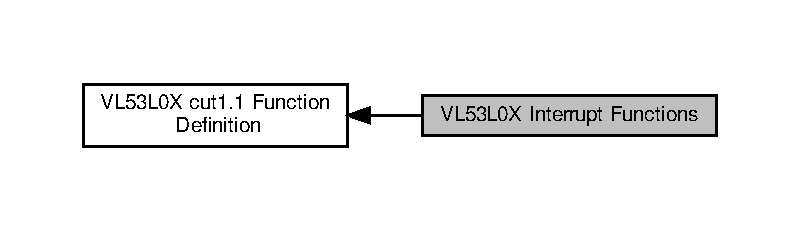
\includegraphics[width=350pt]{group__VL53L0X__interrupt__group}
\end{center}
\end{figure}
\subsection*{Functions}
\begin{DoxyCompactItemize}
\item 
V\+L53\+L0\+X\+\_\+\+A\+PI V\+L53\+L0\+X\+\_\+\+Error \hyperlink{group__VL53L0X__interrupt__group_ga8793fb3c70a2c297247a103e1b446f49}{V\+L53\+L0\+X\+\_\+\+Set\+Gpio\+Config} (\hyperlink{group__VL53L0X__platform__group_ga2d6405308b1dd524b462f1b8fb97d167}{V\+L53\+L0\+X\+\_\+\+D\+EV} Dev, \hyperlink{vl53l0x__types_8h_aba7bc1797add20fe3efdf37ced1182c5}{uint8\+\_\+t} Pin, V\+L53\+L0\+X\+\_\+\+Device\+Modes Device\+Mode, V\+L53\+L0\+X\+\_\+\+Gpio\+Functionality Functionality, V\+L53\+L0\+X\+\_\+\+Interrupt\+Polarity Polarity)
\begin{DoxyCompactList}\small\item\em Set the configuration of G\+P\+IO pin for a given device. \end{DoxyCompactList}\item 
V\+L53\+L0\+X\+\_\+\+A\+PI V\+L53\+L0\+X\+\_\+\+Error \hyperlink{group__VL53L0X__interrupt__group_gadb505a2440a9e00170bca1da6ca6a50f}{V\+L53\+L0\+X\+\_\+\+Get\+Gpio\+Config} (\hyperlink{group__VL53L0X__platform__group_ga2d6405308b1dd524b462f1b8fb97d167}{V\+L53\+L0\+X\+\_\+\+D\+EV} Dev, \hyperlink{vl53l0x__types_8h_aba7bc1797add20fe3efdf37ced1182c5}{uint8\+\_\+t} Pin, V\+L53\+L0\+X\+\_\+\+Device\+Modes $\ast$p\+Device\+Mode, V\+L53\+L0\+X\+\_\+\+Gpio\+Functionality $\ast$p\+Functionality, V\+L53\+L0\+X\+\_\+\+Interrupt\+Polarity $\ast$p\+Polarity)
\begin{DoxyCompactList}\small\item\em Get current configuration for G\+P\+IO pin for a given device. \end{DoxyCompactList}\item 
V\+L53\+L0\+X\+\_\+\+A\+PI V\+L53\+L0\+X\+\_\+\+Error \hyperlink{group__VL53L0X__interrupt__group_ga3c49d83194d278e3a2706ee1732e28de}{V\+L53\+L0\+X\+\_\+\+Set\+Interrupt\+Thresholds} (\hyperlink{group__VL53L0X__platform__group_ga2d6405308b1dd524b462f1b8fb97d167}{V\+L53\+L0\+X\+\_\+\+D\+EV} Dev, V\+L53\+L0\+X\+\_\+\+Device\+Modes Device\+Mode, \hyperlink{vl53l0x__types_8h_afb910790161809fc76e1a274a6349384}{Fix\+Point1616\+\_\+t} Threshold\+Low, \hyperlink{vl53l0x__types_8h_afb910790161809fc76e1a274a6349384}{Fix\+Point1616\+\_\+t} Threshold\+High)
\begin{DoxyCompactList}\small\item\em Set low and high Interrupt thresholds for a given mode (ranging, A\+LS, ...) for a given device. \end{DoxyCompactList}\item 
V\+L53\+L0\+X\+\_\+\+A\+PI V\+L53\+L0\+X\+\_\+\+Error \hyperlink{group__VL53L0X__interrupt__group_ga9d1025202afa35f30ec8efc1ab42b65d}{V\+L53\+L0\+X\+\_\+\+Get\+Interrupt\+Thresholds} (\hyperlink{group__VL53L0X__platform__group_ga2d6405308b1dd524b462f1b8fb97d167}{V\+L53\+L0\+X\+\_\+\+D\+EV} Dev, V\+L53\+L0\+X\+\_\+\+Device\+Modes Device\+Mode, \hyperlink{vl53l0x__types_8h_afb910790161809fc76e1a274a6349384}{Fix\+Point1616\+\_\+t} $\ast$p\+Threshold\+Low, \hyperlink{vl53l0x__types_8h_afb910790161809fc76e1a274a6349384}{Fix\+Point1616\+\_\+t} $\ast$p\+Threshold\+High)
\begin{DoxyCompactList}\small\item\em Get high and low Interrupt thresholds for a given mode (ranging, A\+LS, ...) for a given device. \end{DoxyCompactList}\item 
V\+L53\+L0\+X\+\_\+\+A\+PI V\+L53\+L0\+X\+\_\+\+Error \hyperlink{group__VL53L0X__interrupt__group_ga63d96c483cd41f1e679d8144603942cf}{V\+L53\+L0\+X\+\_\+\+Get\+Stop\+Completed\+Status} (\hyperlink{group__VL53L0X__platform__group_ga2d6405308b1dd524b462f1b8fb97d167}{V\+L53\+L0\+X\+\_\+\+D\+EV} Dev, \hyperlink{vl53l0x__types_8h_a435d1572bf3f880d55459d9805097f62}{uint32\+\_\+t} $\ast$p\+Stop\+Status)
\begin{DoxyCompactList}\small\item\em Return device stop completion status. \end{DoxyCompactList}\item 
V\+L53\+L0\+X\+\_\+\+A\+PI V\+L53\+L0\+X\+\_\+\+Error \hyperlink{group__VL53L0X__interrupt__group_gaa84b2cf5cd87b118b9a43e7ae764447e}{V\+L53\+L0\+X\+\_\+\+Clear\+Interrupt\+Mask} (\hyperlink{group__VL53L0X__platform__group_ga2d6405308b1dd524b462f1b8fb97d167}{V\+L53\+L0\+X\+\_\+\+D\+EV} Dev, \hyperlink{vl53l0x__types_8h_a435d1572bf3f880d55459d9805097f62}{uint32\+\_\+t} Interrupt\+Mask)
\begin{DoxyCompactList}\small\item\em Clear given system interrupt condition. \end{DoxyCompactList}\item 
V\+L53\+L0\+X\+\_\+\+A\+PI V\+L53\+L0\+X\+\_\+\+Error \hyperlink{group__VL53L0X__interrupt__group_ga8c91d3c30fae1e4c76f6aa3794cab364}{V\+L53\+L0\+X\+\_\+\+Get\+Interrupt\+Mask\+Status} (\hyperlink{group__VL53L0X__platform__group_ga2d6405308b1dd524b462f1b8fb97d167}{V\+L53\+L0\+X\+\_\+\+D\+EV} Dev, \hyperlink{vl53l0x__types_8h_a435d1572bf3f880d55459d9805097f62}{uint32\+\_\+t} $\ast$p\+Interrupt\+Mask\+Status)
\begin{DoxyCompactList}\small\item\em Return device interrupt status. \end{DoxyCompactList}\item 
V\+L53\+L0\+X\+\_\+\+A\+PI V\+L53\+L0\+X\+\_\+\+Error \hyperlink{group__VL53L0X__interrupt__group_ga882a69f683b24cb8102a5071ed0becf7}{V\+L53\+L0\+X\+\_\+\+Enable\+Interrupt\+Mask} (\hyperlink{group__VL53L0X__platform__group_ga2d6405308b1dd524b462f1b8fb97d167}{V\+L53\+L0\+X\+\_\+\+D\+EV} Dev, \hyperlink{vl53l0x__types_8h_a435d1572bf3f880d55459d9805097f62}{uint32\+\_\+t} Interrupt\+Mask)
\begin{DoxyCompactList}\small\item\em Configure ranging interrupt reported to system. \end{DoxyCompactList}\end{DoxyCompactItemize}


\subsection{Detailed Description}
Functions used for interrupt managements. 



\subsection{Function Documentation}
\mbox{\Hypertarget{group__VL53L0X__interrupt__group_gaa84b2cf5cd87b118b9a43e7ae764447e}\label{group__VL53L0X__interrupt__group_gaa84b2cf5cd87b118b9a43e7ae764447e}} 
\index{V\+L53\+L0\+X Interrupt Functions@{V\+L53\+L0\+X Interrupt Functions}!V\+L53\+L0\+X\+\_\+\+Clear\+Interrupt\+Mask@{V\+L53\+L0\+X\+\_\+\+Clear\+Interrupt\+Mask}}
\index{V\+L53\+L0\+X\+\_\+\+Clear\+Interrupt\+Mask@{V\+L53\+L0\+X\+\_\+\+Clear\+Interrupt\+Mask}!V\+L53\+L0\+X Interrupt Functions@{V\+L53\+L0\+X Interrupt Functions}}
\subsubsection{\texorpdfstring{V\+L53\+L0\+X\+\_\+\+Clear\+Interrupt\+Mask()}{VL53L0X\_ClearInterruptMask()}}
{\footnotesize\ttfamily V\+L53\+L0\+X\+\_\+\+A\+PI V\+L53\+L0\+X\+\_\+\+Error V\+L53\+L0\+X\+\_\+\+Clear\+Interrupt\+Mask (\begin{DoxyParamCaption}\item[{\hyperlink{group__VL53L0X__platform__group_ga2d6405308b1dd524b462f1b8fb97d167}{V\+L53\+L0\+X\+\_\+\+D\+EV}}]{Dev,  }\item[{\hyperlink{vl53l0x__types_8h_a435d1572bf3f880d55459d9805097f62}{uint32\+\_\+t}}]{Interrupt\+Mask }\end{DoxyParamCaption})}



Clear given system interrupt condition. 

\begin{DoxyParagraph}{Function Description}
Clear given interrupt(s).
\end{DoxyParagraph}
\begin{DoxyNote}{Note}
This function Access to the device
\end{DoxyNote}

\begin{DoxyParams}{Parameters}
{\em Dev} & Device Handle \\
\hline
{\em Interrupt\+Mask} & Mask of interrupts to clear \\
\hline
\end{DoxyParams}
\begin{DoxyReturn}{Returns}
V\+L53\+L0\+X\+\_\+\+E\+R\+R\+O\+R\+\_\+\+N\+O\+NE Success 

V\+L53\+L0\+X\+\_\+\+E\+R\+R\+O\+R\+\_\+\+I\+N\+T\+E\+R\+R\+U\+P\+T\+\_\+\+N\+O\+T\+\_\+\+C\+L\+E\+A\+R\+ED Cannot clear interrupts

\char`\"{}\+Other error code\char`\"{} See \+::\+V\+L53\+L0\+X\+\_\+\+Error 
\end{DoxyReturn}
\mbox{\Hypertarget{group__VL53L0X__interrupt__group_ga882a69f683b24cb8102a5071ed0becf7}\label{group__VL53L0X__interrupt__group_ga882a69f683b24cb8102a5071ed0becf7}} 
\index{V\+L53\+L0\+X Interrupt Functions@{V\+L53\+L0\+X Interrupt Functions}!V\+L53\+L0\+X\+\_\+\+Enable\+Interrupt\+Mask@{V\+L53\+L0\+X\+\_\+\+Enable\+Interrupt\+Mask}}
\index{V\+L53\+L0\+X\+\_\+\+Enable\+Interrupt\+Mask@{V\+L53\+L0\+X\+\_\+\+Enable\+Interrupt\+Mask}!V\+L53\+L0\+X Interrupt Functions@{V\+L53\+L0\+X Interrupt Functions}}
\subsubsection{\texorpdfstring{V\+L53\+L0\+X\+\_\+\+Enable\+Interrupt\+Mask()}{VL53L0X\_EnableInterruptMask()}}
{\footnotesize\ttfamily V\+L53\+L0\+X\+\_\+\+A\+PI V\+L53\+L0\+X\+\_\+\+Error V\+L53\+L0\+X\+\_\+\+Enable\+Interrupt\+Mask (\begin{DoxyParamCaption}\item[{\hyperlink{group__VL53L0X__platform__group_ga2d6405308b1dd524b462f1b8fb97d167}{V\+L53\+L0\+X\+\_\+\+D\+EV}}]{Dev,  }\item[{\hyperlink{vl53l0x__types_8h_a435d1572bf3f880d55459d9805097f62}{uint32\+\_\+t}}]{Interrupt\+Mask }\end{DoxyParamCaption})}



Configure ranging interrupt reported to system. 

\begin{DoxyNote}{Note}
This function is not Implemented
\end{DoxyNote}

\begin{DoxyParams}{Parameters}
{\em Dev} & Device Handle \\
\hline
{\em Interrupt\+Mask} & Mask of interrupt to Enable/disable (0\+:interrupt disabled or 1\+: interrupt enabled) \\
\hline
\end{DoxyParams}
\begin{DoxyReturn}{Returns}
V\+L53\+L0\+X\+\_\+\+E\+R\+R\+O\+R\+\_\+\+N\+O\+T\+\_\+\+I\+M\+P\+L\+E\+M\+E\+N\+T\+ED Not implemented 
\end{DoxyReturn}
\mbox{\Hypertarget{group__VL53L0X__interrupt__group_gadb505a2440a9e00170bca1da6ca6a50f}\label{group__VL53L0X__interrupt__group_gadb505a2440a9e00170bca1da6ca6a50f}} 
\index{V\+L53\+L0\+X Interrupt Functions@{V\+L53\+L0\+X Interrupt Functions}!V\+L53\+L0\+X\+\_\+\+Get\+Gpio\+Config@{V\+L53\+L0\+X\+\_\+\+Get\+Gpio\+Config}}
\index{V\+L53\+L0\+X\+\_\+\+Get\+Gpio\+Config@{V\+L53\+L0\+X\+\_\+\+Get\+Gpio\+Config}!V\+L53\+L0\+X Interrupt Functions@{V\+L53\+L0\+X Interrupt Functions}}
\subsubsection{\texorpdfstring{V\+L53\+L0\+X\+\_\+\+Get\+Gpio\+Config()}{VL53L0X\_GetGpioConfig()}}
{\footnotesize\ttfamily V\+L53\+L0\+X\+\_\+\+A\+PI V\+L53\+L0\+X\+\_\+\+Error V\+L53\+L0\+X\+\_\+\+Get\+Gpio\+Config (\begin{DoxyParamCaption}\item[{\hyperlink{group__VL53L0X__platform__group_ga2d6405308b1dd524b462f1b8fb97d167}{V\+L53\+L0\+X\+\_\+\+D\+EV}}]{Dev,  }\item[{\hyperlink{vl53l0x__types_8h_aba7bc1797add20fe3efdf37ced1182c5}{uint8\+\_\+t}}]{Pin,  }\item[{V\+L53\+L0\+X\+\_\+\+Device\+Modes $\ast$}]{p\+Device\+Mode,  }\item[{V\+L53\+L0\+X\+\_\+\+Gpio\+Functionality $\ast$}]{p\+Functionality,  }\item[{V\+L53\+L0\+X\+\_\+\+Interrupt\+Polarity $\ast$}]{p\+Polarity }\end{DoxyParamCaption})}



Get current configuration for G\+P\+IO pin for a given device. 

\begin{DoxyNote}{Note}
This function Access to the device
\end{DoxyNote}

\begin{DoxyParams}{Parameters}
{\em Dev} & Device Handle \\
\hline
{\em Pin} & ID of the G\+P\+IO Pin \\
\hline
{\em p\+Device\+Mode} & Pointer to Device Mode associated to the Gpio. \\
\hline
{\em p\+Functionality} & Pointer to Pin functionality. Refer to \+::\+V\+L53\+L0\+X\+\_\+\+Gpio\+Functionality \\
\hline
{\em p\+Polarity} & Pointer to interrupt polarity. Active high or active low see \+::\+V\+L53\+L0\+X\+\_\+\+Interrupt\+Polarity \\
\hline
\end{DoxyParams}
\begin{DoxyReturn}{Returns}
V\+L53\+L0\+X\+\_\+\+E\+R\+R\+O\+R\+\_\+\+N\+O\+NE Success 

V\+L53\+L0\+X\+\_\+\+E\+R\+R\+O\+R\+\_\+\+G\+P\+I\+O\+\_\+\+N\+O\+T\+\_\+\+E\+X\+I\+S\+T\+I\+NG Only Pin=0 is accepted. 

V\+L53\+L0\+X\+\_\+\+E\+R\+R\+O\+R\+\_\+\+G\+P\+I\+O\+\_\+\+F\+U\+N\+C\+T\+I\+O\+N\+A\+L\+I\+T\+Y\+\_\+\+N\+O\+T\+\_\+\+S\+U\+P\+P\+O\+R\+T\+ED This error occurs when Functionality programmed is not in the supported list\+: Supported value are\+: V\+L53\+L0\+X\+\_\+\+G\+P\+I\+O\+F\+U\+N\+C\+T\+I\+O\+N\+A\+L\+I\+T\+Y\+\_\+\+O\+FF, V\+L53\+L0\+X\+\_\+\+G\+P\+I\+O\+F\+U\+N\+C\+T\+I\+O\+N\+A\+L\+I\+T\+Y\+\_\+\+T\+H\+R\+E\+S\+H\+O\+L\+D\+\_\+\+C\+R\+O\+S\+S\+E\+D\+\_\+\+L\+OW, V\+L53\+L0\+X\+\_\+\+G\+P\+I\+O\+F\+U\+N\+C\+T\+I\+O\+N\+A\+L\+I\+T\+Y\+\_\+\+T\+H\+R\+E\+S\+H\+O\+L\+D\+\_\+\+C\+R\+O\+S\+S\+E\+D\+\_\+\+H\+I\+GH, V\+L53\+L0\+X\+\_\+\+G\+P\+I\+O\+F\+U\+N\+C\+T\+I\+O\+N\+A\+L\+I\+T\+Y\+\_\+\+T\+H\+R\+E\+S\+H\+O\+L\+D\+\_\+\+C\+R\+O\+S\+S\+E\+D\+\_\+\+O\+UT, V\+L53\+L0\+X\+\_\+\+G\+P\+I\+O\+F\+U\+N\+C\+T\+I\+O\+N\+A\+L\+I\+T\+Y\+\_\+\+N\+E\+W\+\_\+\+M\+E\+A\+S\+U\+R\+E\+\_\+\+R\+E\+A\+DY 

\char`\"{}\+Other error code\char`\"{} See \+::\+V\+L53\+L0\+X\+\_\+\+Error 
\end{DoxyReturn}
\mbox{\Hypertarget{group__VL53L0X__interrupt__group_ga8c91d3c30fae1e4c76f6aa3794cab364}\label{group__VL53L0X__interrupt__group_ga8c91d3c30fae1e4c76f6aa3794cab364}} 
\index{V\+L53\+L0\+X Interrupt Functions@{V\+L53\+L0\+X Interrupt Functions}!V\+L53\+L0\+X\+\_\+\+Get\+Interrupt\+Mask\+Status@{V\+L53\+L0\+X\+\_\+\+Get\+Interrupt\+Mask\+Status}}
\index{V\+L53\+L0\+X\+\_\+\+Get\+Interrupt\+Mask\+Status@{V\+L53\+L0\+X\+\_\+\+Get\+Interrupt\+Mask\+Status}!V\+L53\+L0\+X Interrupt Functions@{V\+L53\+L0\+X Interrupt Functions}}
\subsubsection{\texorpdfstring{V\+L53\+L0\+X\+\_\+\+Get\+Interrupt\+Mask\+Status()}{VL53L0X\_GetInterruptMaskStatus()}}
{\footnotesize\ttfamily V\+L53\+L0\+X\+\_\+\+A\+PI V\+L53\+L0\+X\+\_\+\+Error V\+L53\+L0\+X\+\_\+\+Get\+Interrupt\+Mask\+Status (\begin{DoxyParamCaption}\item[{\hyperlink{group__VL53L0X__platform__group_ga2d6405308b1dd524b462f1b8fb97d167}{V\+L53\+L0\+X\+\_\+\+D\+EV}}]{Dev,  }\item[{\hyperlink{vl53l0x__types_8h_a435d1572bf3f880d55459d9805097f62}{uint32\+\_\+t} $\ast$}]{p\+Interrupt\+Mask\+Status }\end{DoxyParamCaption})}



Return device interrupt status. 

\begin{DoxyParagraph}{Function Description}
Returns currently raised interrupts by the device. User shall be able to activate/deactivate interrupts through {\itshape \hyperlink{group__VL53L0X__interrupt__group_ga8793fb3c70a2c297247a103e1b446f49}{V\+L53\+L0\+X\+\_\+\+Set\+Gpio\+Config()}} 
\end{DoxyParagraph}
\begin{DoxyNote}{Note}
This function Access to the device
\end{DoxyNote}

\begin{DoxyParams}{Parameters}
{\em Dev} & Device Handle \\
\hline
{\em p\+Interrupt\+Mask\+Status} & Pointer to status variable to update \\
\hline
\end{DoxyParams}
\begin{DoxyReturn}{Returns}
V\+L53\+L0\+X\+\_\+\+E\+R\+R\+O\+R\+\_\+\+N\+O\+NE Success 

\char`\"{}\+Other error code\char`\"{} See \+::\+V\+L53\+L0\+X\+\_\+\+Error 
\end{DoxyReturn}
\mbox{\Hypertarget{group__VL53L0X__interrupt__group_ga9d1025202afa35f30ec8efc1ab42b65d}\label{group__VL53L0X__interrupt__group_ga9d1025202afa35f30ec8efc1ab42b65d}} 
\index{V\+L53\+L0\+X Interrupt Functions@{V\+L53\+L0\+X Interrupt Functions}!V\+L53\+L0\+X\+\_\+\+Get\+Interrupt\+Thresholds@{V\+L53\+L0\+X\+\_\+\+Get\+Interrupt\+Thresholds}}
\index{V\+L53\+L0\+X\+\_\+\+Get\+Interrupt\+Thresholds@{V\+L53\+L0\+X\+\_\+\+Get\+Interrupt\+Thresholds}!V\+L53\+L0\+X Interrupt Functions@{V\+L53\+L0\+X Interrupt Functions}}
\subsubsection{\texorpdfstring{V\+L53\+L0\+X\+\_\+\+Get\+Interrupt\+Thresholds()}{VL53L0X\_GetInterruptThresholds()}}
{\footnotesize\ttfamily V\+L53\+L0\+X\+\_\+\+A\+PI V\+L53\+L0\+X\+\_\+\+Error V\+L53\+L0\+X\+\_\+\+Get\+Interrupt\+Thresholds (\begin{DoxyParamCaption}\item[{\hyperlink{group__VL53L0X__platform__group_ga2d6405308b1dd524b462f1b8fb97d167}{V\+L53\+L0\+X\+\_\+\+D\+EV}}]{Dev,  }\item[{V\+L53\+L0\+X\+\_\+\+Device\+Modes}]{Device\+Mode,  }\item[{\hyperlink{vl53l0x__types_8h_afb910790161809fc76e1a274a6349384}{Fix\+Point1616\+\_\+t} $\ast$}]{p\+Threshold\+Low,  }\item[{\hyperlink{vl53l0x__types_8h_afb910790161809fc76e1a274a6349384}{Fix\+Point1616\+\_\+t} $\ast$}]{p\+Threshold\+High }\end{DoxyParamCaption})}



Get high and low Interrupt thresholds for a given mode (ranging, A\+LS, ...) for a given device. 

\begin{DoxyParagraph}{Function Description}
Get high and low Interrupt thresholds for a given mode (ranging, A\+LS, ...) for a given device
\end{DoxyParagraph}
\begin{DoxyNote}{Note}
This function Access to the device

Device\+Mode is ignored for the current device
\end{DoxyNote}

\begin{DoxyParams}{Parameters}
{\em Dev} & Device Handle \\
\hline
{\em Device\+Mode} & Device Mode from which read thresholds \\
\hline
{\em p\+Threshold\+Low} & Low threshold (mm, lux ..., depending on the mode) \\
\hline
{\em p\+Threshold\+High} & High threshold (mm, lux ..., depending on the mode) \\
\hline
\end{DoxyParams}
\begin{DoxyReturn}{Returns}
V\+L53\+L0\+X\+\_\+\+E\+R\+R\+O\+R\+\_\+\+N\+O\+NE Success 

\char`\"{}\+Other error code\char`\"{} See \+::\+V\+L53\+L0\+X\+\_\+\+Error 
\end{DoxyReturn}
\mbox{\Hypertarget{group__VL53L0X__interrupt__group_ga63d96c483cd41f1e679d8144603942cf}\label{group__VL53L0X__interrupt__group_ga63d96c483cd41f1e679d8144603942cf}} 
\index{V\+L53\+L0\+X Interrupt Functions@{V\+L53\+L0\+X Interrupt Functions}!V\+L53\+L0\+X\+\_\+\+Get\+Stop\+Completed\+Status@{V\+L53\+L0\+X\+\_\+\+Get\+Stop\+Completed\+Status}}
\index{V\+L53\+L0\+X\+\_\+\+Get\+Stop\+Completed\+Status@{V\+L53\+L0\+X\+\_\+\+Get\+Stop\+Completed\+Status}!V\+L53\+L0\+X Interrupt Functions@{V\+L53\+L0\+X Interrupt Functions}}
\subsubsection{\texorpdfstring{V\+L53\+L0\+X\+\_\+\+Get\+Stop\+Completed\+Status()}{VL53L0X\_GetStopCompletedStatus()}}
{\footnotesize\ttfamily V\+L53\+L0\+X\+\_\+\+A\+PI V\+L53\+L0\+X\+\_\+\+Error V\+L53\+L0\+X\+\_\+\+Get\+Stop\+Completed\+Status (\begin{DoxyParamCaption}\item[{\hyperlink{group__VL53L0X__platform__group_ga2d6405308b1dd524b462f1b8fb97d167}{V\+L53\+L0\+X\+\_\+\+D\+EV}}]{Dev,  }\item[{\hyperlink{vl53l0x__types_8h_a435d1572bf3f880d55459d9805097f62}{uint32\+\_\+t} $\ast$}]{p\+Stop\+Status }\end{DoxyParamCaption})}



Return device stop completion status. 

\begin{DoxyParagraph}{Function Description}
Returns stop completiob status. User shall call this function after a stop command
\end{DoxyParagraph}
\begin{DoxyNote}{Note}
This function Access to the device
\end{DoxyNote}

\begin{DoxyParams}{Parameters}
{\em Dev} & Device Handle \\
\hline
{\em p\+Stop\+Status} & Pointer to status variable to update \\
\hline
\end{DoxyParams}
\begin{DoxyReturn}{Returns}
V\+L53\+L0\+X\+\_\+\+E\+R\+R\+O\+R\+\_\+\+N\+O\+NE Success 

\char`\"{}\+Other error code\char`\"{} See \+::\+V\+L53\+L0\+X\+\_\+\+Error 
\end{DoxyReturn}
\mbox{\Hypertarget{group__VL53L0X__interrupt__group_ga8793fb3c70a2c297247a103e1b446f49}\label{group__VL53L0X__interrupt__group_ga8793fb3c70a2c297247a103e1b446f49}} 
\index{V\+L53\+L0\+X Interrupt Functions@{V\+L53\+L0\+X Interrupt Functions}!V\+L53\+L0\+X\+\_\+\+Set\+Gpio\+Config@{V\+L53\+L0\+X\+\_\+\+Set\+Gpio\+Config}}
\index{V\+L53\+L0\+X\+\_\+\+Set\+Gpio\+Config@{V\+L53\+L0\+X\+\_\+\+Set\+Gpio\+Config}!V\+L53\+L0\+X Interrupt Functions@{V\+L53\+L0\+X Interrupt Functions}}
\subsubsection{\texorpdfstring{V\+L53\+L0\+X\+\_\+\+Set\+Gpio\+Config()}{VL53L0X\_SetGpioConfig()}}
{\footnotesize\ttfamily V\+L53\+L0\+X\+\_\+\+A\+PI V\+L53\+L0\+X\+\_\+\+Error V\+L53\+L0\+X\+\_\+\+Set\+Gpio\+Config (\begin{DoxyParamCaption}\item[{\hyperlink{group__VL53L0X__platform__group_ga2d6405308b1dd524b462f1b8fb97d167}{V\+L53\+L0\+X\+\_\+\+D\+EV}}]{Dev,  }\item[{\hyperlink{vl53l0x__types_8h_aba7bc1797add20fe3efdf37ced1182c5}{uint8\+\_\+t}}]{Pin,  }\item[{V\+L53\+L0\+X\+\_\+\+Device\+Modes}]{Device\+Mode,  }\item[{V\+L53\+L0\+X\+\_\+\+Gpio\+Functionality}]{Functionality,  }\item[{V\+L53\+L0\+X\+\_\+\+Interrupt\+Polarity}]{Polarity }\end{DoxyParamCaption})}



Set the configuration of G\+P\+IO pin for a given device. 

\begin{DoxyNote}{Note}
This function Access to the device
\end{DoxyNote}

\begin{DoxyParams}{Parameters}
{\em Dev} & Device Handle \\
\hline
{\em Pin} & ID of the G\+P\+IO Pin \\
\hline
{\em Functionality} & Select Pin functionality. Refer to \+::\+V\+L53\+L0\+X\+\_\+\+Gpio\+Functionality \\
\hline
{\em Device\+Mode} & Device Mode associated to the Gpio. \\
\hline
{\em Polarity} & Set interrupt polarity. Active high or active low see \+::\+V\+L53\+L0\+X\+\_\+\+Interrupt\+Polarity \\
\hline
\end{DoxyParams}
\begin{DoxyReturn}{Returns}
V\+L53\+L0\+X\+\_\+\+E\+R\+R\+O\+R\+\_\+\+N\+O\+NE Success 

V\+L53\+L0\+X\+\_\+\+E\+R\+R\+O\+R\+\_\+\+G\+P\+I\+O\+\_\+\+N\+O\+T\+\_\+\+E\+X\+I\+S\+T\+I\+NG Only Pin=0 is accepted. 

V\+L53\+L0\+X\+\_\+\+E\+R\+R\+O\+R\+\_\+\+G\+P\+I\+O\+\_\+\+F\+U\+N\+C\+T\+I\+O\+N\+A\+L\+I\+T\+Y\+\_\+\+N\+O\+T\+\_\+\+S\+U\+P\+P\+O\+R\+T\+ED This error occurs when Functionality programmed is not in the supported list\+: Supported value are\+: V\+L53\+L0\+X\+\_\+\+G\+P\+I\+O\+F\+U\+N\+C\+T\+I\+O\+N\+A\+L\+I\+T\+Y\+\_\+\+O\+FF, V\+L53\+L0\+X\+\_\+\+G\+P\+I\+O\+F\+U\+N\+C\+T\+I\+O\+N\+A\+L\+I\+T\+Y\+\_\+\+T\+H\+R\+E\+S\+H\+O\+L\+D\+\_\+\+C\+R\+O\+S\+S\+E\+D\+\_\+\+L\+OW, V\+L53\+L0\+X\+\_\+\+G\+P\+I\+O\+F\+U\+N\+C\+T\+I\+O\+N\+A\+L\+I\+T\+Y\+\_\+\+T\+H\+R\+E\+S\+H\+O\+L\+D\+\_\+\+C\+R\+O\+S\+S\+E\+D\+\_\+\+H\+I\+GH, V\+L53\+L0\+X\+\_\+\+G\+P\+I\+O\+F\+U\+N\+C\+T\+I\+O\+N\+A\+L\+I\+T\+Y\+\_\+\+T\+H\+R\+E\+S\+H\+O\+L\+D\+\_\+\+C\+R\+O\+S\+S\+E\+D\+\_\+\+O\+UT, V\+L53\+L0\+X\+\_\+\+G\+P\+I\+O\+F\+U\+N\+C\+T\+I\+O\+N\+A\+L\+I\+T\+Y\+\_\+\+N\+E\+W\+\_\+\+M\+E\+A\+S\+U\+R\+E\+\_\+\+R\+E\+A\+DY 

\char`\"{}\+Other error code\char`\"{} See \+::\+V\+L53\+L0\+X\+\_\+\+Error 
\end{DoxyReturn}
\mbox{\Hypertarget{group__VL53L0X__interrupt__group_ga3c49d83194d278e3a2706ee1732e28de}\label{group__VL53L0X__interrupt__group_ga3c49d83194d278e3a2706ee1732e28de}} 
\index{V\+L53\+L0\+X Interrupt Functions@{V\+L53\+L0\+X Interrupt Functions}!V\+L53\+L0\+X\+\_\+\+Set\+Interrupt\+Thresholds@{V\+L53\+L0\+X\+\_\+\+Set\+Interrupt\+Thresholds}}
\index{V\+L53\+L0\+X\+\_\+\+Set\+Interrupt\+Thresholds@{V\+L53\+L0\+X\+\_\+\+Set\+Interrupt\+Thresholds}!V\+L53\+L0\+X Interrupt Functions@{V\+L53\+L0\+X Interrupt Functions}}
\subsubsection{\texorpdfstring{V\+L53\+L0\+X\+\_\+\+Set\+Interrupt\+Thresholds()}{VL53L0X\_SetInterruptThresholds()}}
{\footnotesize\ttfamily V\+L53\+L0\+X\+\_\+\+A\+PI V\+L53\+L0\+X\+\_\+\+Error V\+L53\+L0\+X\+\_\+\+Set\+Interrupt\+Thresholds (\begin{DoxyParamCaption}\item[{\hyperlink{group__VL53L0X__platform__group_ga2d6405308b1dd524b462f1b8fb97d167}{V\+L53\+L0\+X\+\_\+\+D\+EV}}]{Dev,  }\item[{V\+L53\+L0\+X\+\_\+\+Device\+Modes}]{Device\+Mode,  }\item[{\hyperlink{vl53l0x__types_8h_afb910790161809fc76e1a274a6349384}{Fix\+Point1616\+\_\+t}}]{Threshold\+Low,  }\item[{\hyperlink{vl53l0x__types_8h_afb910790161809fc76e1a274a6349384}{Fix\+Point1616\+\_\+t}}]{Threshold\+High }\end{DoxyParamCaption})}



Set low and high Interrupt thresholds for a given mode (ranging, A\+LS, ...) for a given device. 

\begin{DoxyParagraph}{Function Description}
Set low and high Interrupt thresholds for a given mode (ranging, A\+LS, ...) for a given device
\end{DoxyParagraph}
\begin{DoxyNote}{Note}
This function Access to the device

Device\+Mode is ignored for the current device
\end{DoxyNote}

\begin{DoxyParams}{Parameters}
{\em Dev} & Device Handle \\
\hline
{\em Device\+Mode} & Device Mode for which change thresholds \\
\hline
{\em Threshold\+Low} & Low threshold (mm, lux ..., depending on the mode) \\
\hline
{\em Threshold\+High} & High threshold (mm, lux ..., depending on the mode) \\
\hline
\end{DoxyParams}
\begin{DoxyReturn}{Returns}
V\+L53\+L0\+X\+\_\+\+E\+R\+R\+O\+R\+\_\+\+N\+O\+NE Success 

\char`\"{}\+Other error code\char`\"{} See \+::\+V\+L53\+L0\+X\+\_\+\+Error 
\end{DoxyReturn}

\hypertarget{group__VL53L0X__SPADfunctions__group}{}\section{V\+L53\+L0X S\+P\+AD Functions}
\label{group__VL53L0X__SPADfunctions__group}\index{V\+L53\+L0\+X S\+P\+A\+D Functions@{V\+L53\+L0\+X S\+P\+A\+D Functions}}


Functions used for S\+P\+AD managements.  


Collaboration diagram for V\+L53\+L0X S\+P\+AD Functions\+:\nopagebreak
\begin{figure}[H]
\begin{center}
\leavevmode
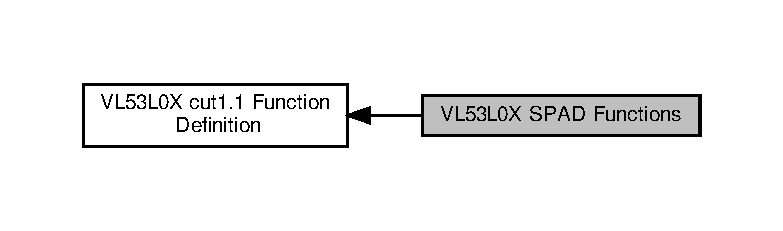
\includegraphics[width=350pt]{group__VL53L0X__SPADfunctions__group}
\end{center}
\end{figure}
\subsection*{Functions}
\begin{DoxyCompactItemize}
\item 
V\+L53\+L0\+X\+\_\+\+A\+PI V\+L53\+L0\+X\+\_\+\+Error \hyperlink{group__VL53L0X__SPADfunctions__group_ga989a7fd1772142cc2d4d63d6f3d0fb7e}{V\+L53\+L0\+X\+\_\+\+Set\+Spad\+Ambient\+Damper\+Threshold} (\hyperlink{group__VL53L0X__platform__group_ga2d6405308b1dd524b462f1b8fb97d167}{V\+L53\+L0\+X\+\_\+\+D\+EV} Dev, \hyperlink{vl53l0x__types_8h_a273cf69d639a59973b6019625df33e30}{uint16\+\_\+t} Spad\+Ambient\+Damper\+Threshold)
\begin{DoxyCompactList}\small\item\em Set the S\+P\+AD Ambient Damper Threshold value. \end{DoxyCompactList}\item 
V\+L53\+L0\+X\+\_\+\+A\+PI V\+L53\+L0\+X\+\_\+\+Error \hyperlink{group__VL53L0X__SPADfunctions__group_gab4242560466b011b4932f0df18b5ad1a}{V\+L53\+L0\+X\+\_\+\+Get\+Spad\+Ambient\+Damper\+Threshold} (\hyperlink{group__VL53L0X__platform__group_ga2d6405308b1dd524b462f1b8fb97d167}{V\+L53\+L0\+X\+\_\+\+D\+EV} Dev, \hyperlink{vl53l0x__types_8h_a273cf69d639a59973b6019625df33e30}{uint16\+\_\+t} $\ast$p\+Spad\+Ambient\+Damper\+Threshold)
\begin{DoxyCompactList}\small\item\em Get the current S\+P\+AD Ambient Damper Threshold value. \end{DoxyCompactList}\item 
V\+L53\+L0\+X\+\_\+\+A\+PI V\+L53\+L0\+X\+\_\+\+Error \hyperlink{group__VL53L0X__SPADfunctions__group_ga8b17c5364d68ff87f3f99a8292db59d7}{V\+L53\+L0\+X\+\_\+\+Set\+Spad\+Ambient\+Damper\+Factor} (\hyperlink{group__VL53L0X__platform__group_ga2d6405308b1dd524b462f1b8fb97d167}{V\+L53\+L0\+X\+\_\+\+D\+EV} Dev, \hyperlink{vl53l0x__types_8h_a273cf69d639a59973b6019625df33e30}{uint16\+\_\+t} Spad\+Ambient\+Damper\+Factor)
\begin{DoxyCompactList}\small\item\em Set the S\+P\+AD Ambient Damper Factor value. \end{DoxyCompactList}\item 
V\+L53\+L0\+X\+\_\+\+A\+PI V\+L53\+L0\+X\+\_\+\+Error \hyperlink{group__VL53L0X__SPADfunctions__group_gaf43dba72f3295ec5d0334d5712d122ce}{V\+L53\+L0\+X\+\_\+\+Get\+Spad\+Ambient\+Damper\+Factor} (\hyperlink{group__VL53L0X__platform__group_ga2d6405308b1dd524b462f1b8fb97d167}{V\+L53\+L0\+X\+\_\+\+D\+EV} Dev, \hyperlink{vl53l0x__types_8h_a273cf69d639a59973b6019625df33e30}{uint16\+\_\+t} $\ast$p\+Spad\+Ambient\+Damper\+Factor)
\begin{DoxyCompactList}\small\item\em Get the current S\+P\+AD Ambient Damper Factor value. \end{DoxyCompactList}\item 
V\+L53\+L0\+X\+\_\+\+A\+PI V\+L53\+L0\+X\+\_\+\+Error \hyperlink{group__VL53L0X__SPADfunctions__group_ga70e6eb20975784b72296874674a57bbb}{V\+L53\+L0\+X\+\_\+\+Perform\+Ref\+Spad\+Management} (\hyperlink{group__VL53L0X__platform__group_ga2d6405308b1dd524b462f1b8fb97d167}{V\+L53\+L0\+X\+\_\+\+D\+EV} Dev, \hyperlink{vl53l0x__types_8h_a435d1572bf3f880d55459d9805097f62}{uint32\+\_\+t} $\ast$ref\+Spad\+Count, \hyperlink{vl53l0x__types_8h_aba7bc1797add20fe3efdf37ced1182c5}{uint8\+\_\+t} $\ast$is\+Aperture\+Spads)
\begin{DoxyCompactList}\small\item\em Performs Reference Spad Management. \end{DoxyCompactList}\item 
V\+L53\+L0\+X\+\_\+\+A\+PI V\+L53\+L0\+X\+\_\+\+Error \hyperlink{group__VL53L0X__SPADfunctions__group_ga663f1be502ca04ce6a1fea517c58d599}{V\+L53\+L0\+X\+\_\+\+Set\+Reference\+Spads} (\hyperlink{group__VL53L0X__platform__group_ga2d6405308b1dd524b462f1b8fb97d167}{V\+L53\+L0\+X\+\_\+\+D\+EV} Dev, \hyperlink{vl53l0x__types_8h_a435d1572bf3f880d55459d9805097f62}{uint32\+\_\+t} ref\+Spad\+Count, \hyperlink{vl53l0x__types_8h_aba7bc1797add20fe3efdf37ced1182c5}{uint8\+\_\+t} is\+Aperture\+Spads)
\begin{DoxyCompactList}\small\item\em Applies Reference S\+P\+AD configuration. \end{DoxyCompactList}\item 
V\+L53\+L0\+X\+\_\+\+A\+PI V\+L53\+L0\+X\+\_\+\+Error \hyperlink{group__VL53L0X__SPADfunctions__group_ga47d6d7d3c3d8baaadb136e5c57037899}{V\+L53\+L0\+X\+\_\+\+Get\+Reference\+Spads} (\hyperlink{group__VL53L0X__platform__group_ga2d6405308b1dd524b462f1b8fb97d167}{V\+L53\+L0\+X\+\_\+\+D\+EV} Dev, \hyperlink{vl53l0x__types_8h_a435d1572bf3f880d55459d9805097f62}{uint32\+\_\+t} $\ast$ref\+Spad\+Count, \hyperlink{vl53l0x__types_8h_aba7bc1797add20fe3efdf37ced1182c5}{uint8\+\_\+t} $\ast$is\+Aperture\+Spads)
\begin{DoxyCompactList}\small\item\em Retrieves S\+P\+AD configuration. \end{DoxyCompactList}\end{DoxyCompactItemize}


\subsection{Detailed Description}
Functions used for S\+P\+AD managements. 



\subsection{Function Documentation}
\mbox{\Hypertarget{group__VL53L0X__SPADfunctions__group_ga47d6d7d3c3d8baaadb136e5c57037899}\label{group__VL53L0X__SPADfunctions__group_ga47d6d7d3c3d8baaadb136e5c57037899}} 
\index{V\+L53\+L0\+X S\+P\+A\+D Functions@{V\+L53\+L0\+X S\+P\+A\+D Functions}!V\+L53\+L0\+X\+\_\+\+Get\+Reference\+Spads@{V\+L53\+L0\+X\+\_\+\+Get\+Reference\+Spads}}
\index{V\+L53\+L0\+X\+\_\+\+Get\+Reference\+Spads@{V\+L53\+L0\+X\+\_\+\+Get\+Reference\+Spads}!V\+L53\+L0\+X S\+P\+A\+D Functions@{V\+L53\+L0\+X S\+P\+A\+D Functions}}
\subsubsection{\texorpdfstring{V\+L53\+L0\+X\+\_\+\+Get\+Reference\+Spads()}{VL53L0X\_GetReferenceSpads()}}
{\footnotesize\ttfamily V\+L53\+L0\+X\+\_\+\+A\+PI V\+L53\+L0\+X\+\_\+\+Error V\+L53\+L0\+X\+\_\+\+Get\+Reference\+Spads (\begin{DoxyParamCaption}\item[{\hyperlink{group__VL53L0X__platform__group_ga2d6405308b1dd524b462f1b8fb97d167}{V\+L53\+L0\+X\+\_\+\+D\+EV}}]{Dev,  }\item[{\hyperlink{vl53l0x__types_8h_a435d1572bf3f880d55459d9805097f62}{uint32\+\_\+t} $\ast$}]{ref\+Spad\+Count,  }\item[{\hyperlink{vl53l0x__types_8h_aba7bc1797add20fe3efdf37ced1182c5}{uint8\+\_\+t} $\ast$}]{is\+Aperture\+Spads }\end{DoxyParamCaption})}



Retrieves S\+P\+AD configuration. 

\begin{DoxyParagraph}{Function Description}
This function retrieves the current number of applied reference spads and also their type \+: Aperture or Non-\/\+Aperture.
\end{DoxyParagraph}
\begin{DoxyNote}{Note}
This function Access to the device
\end{DoxyNote}

\begin{DoxyParams}{Parameters}
{\em Dev} & Device Handle \\
\hline
{\em ref\+Spad\+Count} & Number ref Spad Count \\
\hline
{\em is\+Aperture\+Spads} & Reports if spads are of type aperture or non-\/aperture. 1\+:=aperture, 0\+:=Non-\/\+Aperture \\
\hline
\end{DoxyParams}
\begin{DoxyReturn}{Returns}
V\+L53\+L0\+X\+\_\+\+E\+R\+R\+O\+R\+\_\+\+N\+O\+NE Success 

V\+L53\+L0\+X\+\_\+\+E\+R\+R\+O\+R\+\_\+\+R\+E\+F\+\_\+\+S\+P\+A\+D\+\_\+\+I\+N\+IT Error in the in the reference spad configuration. 

\char`\"{}\+Other error code\char`\"{} See \+::\+V\+L53\+L0\+X\+\_\+\+Error 
\end{DoxyReturn}
\mbox{\Hypertarget{group__VL53L0X__SPADfunctions__group_gaf43dba72f3295ec5d0334d5712d122ce}\label{group__VL53L0X__SPADfunctions__group_gaf43dba72f3295ec5d0334d5712d122ce}} 
\index{V\+L53\+L0\+X S\+P\+A\+D Functions@{V\+L53\+L0\+X S\+P\+A\+D Functions}!V\+L53\+L0\+X\+\_\+\+Get\+Spad\+Ambient\+Damper\+Factor@{V\+L53\+L0\+X\+\_\+\+Get\+Spad\+Ambient\+Damper\+Factor}}
\index{V\+L53\+L0\+X\+\_\+\+Get\+Spad\+Ambient\+Damper\+Factor@{V\+L53\+L0\+X\+\_\+\+Get\+Spad\+Ambient\+Damper\+Factor}!V\+L53\+L0\+X S\+P\+A\+D Functions@{V\+L53\+L0\+X S\+P\+A\+D Functions}}
\subsubsection{\texorpdfstring{V\+L53\+L0\+X\+\_\+\+Get\+Spad\+Ambient\+Damper\+Factor()}{VL53L0X\_GetSpadAmbientDamperFactor()}}
{\footnotesize\ttfamily V\+L53\+L0\+X\+\_\+\+A\+PI V\+L53\+L0\+X\+\_\+\+Error V\+L53\+L0\+X\+\_\+\+Get\+Spad\+Ambient\+Damper\+Factor (\begin{DoxyParamCaption}\item[{\hyperlink{group__VL53L0X__platform__group_ga2d6405308b1dd524b462f1b8fb97d167}{V\+L53\+L0\+X\+\_\+\+D\+EV}}]{Dev,  }\item[{\hyperlink{vl53l0x__types_8h_a273cf69d639a59973b6019625df33e30}{uint16\+\_\+t} $\ast$}]{p\+Spad\+Ambient\+Damper\+Factor }\end{DoxyParamCaption})}



Get the current S\+P\+AD Ambient Damper Factor value. 

\begin{DoxyParagraph}{Function Description}
This function get the S\+P\+AD Ambient Damper Factor value
\end{DoxyParagraph}
\begin{DoxyNote}{Note}
This function Access to the device
\end{DoxyNote}

\begin{DoxyParams}{Parameters}
{\em Dev} & Device Handle \\
\hline
{\em p\+Spad\+Ambient\+Damper\+Factor} & Pointer to programmed S\+P\+AD Ambient Damper Factor value \\
\hline
\end{DoxyParams}
\begin{DoxyReturn}{Returns}
V\+L53\+L0\+X\+\_\+\+E\+R\+R\+O\+R\+\_\+\+N\+O\+NE Success 

\char`\"{}\+Other error code\char`\"{} See \+::\+V\+L53\+L0\+X\+\_\+\+Error 
\end{DoxyReturn}
\mbox{\Hypertarget{group__VL53L0X__SPADfunctions__group_gab4242560466b011b4932f0df18b5ad1a}\label{group__VL53L0X__SPADfunctions__group_gab4242560466b011b4932f0df18b5ad1a}} 
\index{V\+L53\+L0\+X S\+P\+A\+D Functions@{V\+L53\+L0\+X S\+P\+A\+D Functions}!V\+L53\+L0\+X\+\_\+\+Get\+Spad\+Ambient\+Damper\+Threshold@{V\+L53\+L0\+X\+\_\+\+Get\+Spad\+Ambient\+Damper\+Threshold}}
\index{V\+L53\+L0\+X\+\_\+\+Get\+Spad\+Ambient\+Damper\+Threshold@{V\+L53\+L0\+X\+\_\+\+Get\+Spad\+Ambient\+Damper\+Threshold}!V\+L53\+L0\+X S\+P\+A\+D Functions@{V\+L53\+L0\+X S\+P\+A\+D Functions}}
\subsubsection{\texorpdfstring{V\+L53\+L0\+X\+\_\+\+Get\+Spad\+Ambient\+Damper\+Threshold()}{VL53L0X\_GetSpadAmbientDamperThreshold()}}
{\footnotesize\ttfamily V\+L53\+L0\+X\+\_\+\+A\+PI V\+L53\+L0\+X\+\_\+\+Error V\+L53\+L0\+X\+\_\+\+Get\+Spad\+Ambient\+Damper\+Threshold (\begin{DoxyParamCaption}\item[{\hyperlink{group__VL53L0X__platform__group_ga2d6405308b1dd524b462f1b8fb97d167}{V\+L53\+L0\+X\+\_\+\+D\+EV}}]{Dev,  }\item[{\hyperlink{vl53l0x__types_8h_a273cf69d639a59973b6019625df33e30}{uint16\+\_\+t} $\ast$}]{p\+Spad\+Ambient\+Damper\+Threshold }\end{DoxyParamCaption})}



Get the current S\+P\+AD Ambient Damper Threshold value. 

\begin{DoxyParagraph}{Function Description}
This function get the S\+P\+AD Ambient Damper Threshold value
\end{DoxyParagraph}
\begin{DoxyNote}{Note}
This function Access to the device
\end{DoxyNote}

\begin{DoxyParams}{Parameters}
{\em Dev} & Device Handle \\
\hline
{\em p\+Spad\+Ambient\+Damper\+Threshold} & Pointer to programmed S\+P\+AD Ambient Damper Threshold value \\
\hline
\end{DoxyParams}
\begin{DoxyReturn}{Returns}
V\+L53\+L0\+X\+\_\+\+E\+R\+R\+O\+R\+\_\+\+N\+O\+NE Success 

\char`\"{}\+Other error code\char`\"{} See \+::\+V\+L53\+L0\+X\+\_\+\+Error 
\end{DoxyReturn}
\mbox{\Hypertarget{group__VL53L0X__SPADfunctions__group_ga70e6eb20975784b72296874674a57bbb}\label{group__VL53L0X__SPADfunctions__group_ga70e6eb20975784b72296874674a57bbb}} 
\index{V\+L53\+L0\+X S\+P\+A\+D Functions@{V\+L53\+L0\+X S\+P\+A\+D Functions}!V\+L53\+L0\+X\+\_\+\+Perform\+Ref\+Spad\+Management@{V\+L53\+L0\+X\+\_\+\+Perform\+Ref\+Spad\+Management}}
\index{V\+L53\+L0\+X\+\_\+\+Perform\+Ref\+Spad\+Management@{V\+L53\+L0\+X\+\_\+\+Perform\+Ref\+Spad\+Management}!V\+L53\+L0\+X S\+P\+A\+D Functions@{V\+L53\+L0\+X S\+P\+A\+D Functions}}
\subsubsection{\texorpdfstring{V\+L53\+L0\+X\+\_\+\+Perform\+Ref\+Spad\+Management()}{VL53L0X\_PerformRefSpadManagement()}}
{\footnotesize\ttfamily V\+L53\+L0\+X\+\_\+\+A\+PI V\+L53\+L0\+X\+\_\+\+Error V\+L53\+L0\+X\+\_\+\+Perform\+Ref\+Spad\+Management (\begin{DoxyParamCaption}\item[{\hyperlink{group__VL53L0X__platform__group_ga2d6405308b1dd524b462f1b8fb97d167}{V\+L53\+L0\+X\+\_\+\+D\+EV}}]{Dev,  }\item[{\hyperlink{vl53l0x__types_8h_a435d1572bf3f880d55459d9805097f62}{uint32\+\_\+t} $\ast$}]{ref\+Spad\+Count,  }\item[{\hyperlink{vl53l0x__types_8h_aba7bc1797add20fe3efdf37ced1182c5}{uint8\+\_\+t} $\ast$}]{is\+Aperture\+Spads }\end{DoxyParamCaption})}



Performs Reference Spad Management. 

\begin{DoxyParagraph}{Function Description}
\hyperlink{structThe}{The} reference S\+P\+AD initialization procedure determines the minimum amount of reference spads to be enables to achieve a target reference signal rate and should be performed once during initialization.
\end{DoxyParagraph}
\begin{DoxyNote}{Note}
This function Access to the device

This function change the device mode to V\+L53\+L0\+X\+\_\+\+D\+E\+V\+I\+C\+E\+M\+O\+D\+E\+\_\+\+S\+I\+N\+G\+L\+E\+\_\+\+R\+A\+N\+G\+I\+NG
\end{DoxyNote}

\begin{DoxyParams}{Parameters}
{\em Dev} & Device Handle \\
\hline
{\em ref\+Spad\+Count} & Reports ref Spad Count \\
\hline
{\em is\+Aperture\+Spads} & Reports if spads are of type aperture or non-\/aperture. 1\+:=aperture, 0\+:=Non-\/\+Aperture \\
\hline
\end{DoxyParams}
\begin{DoxyReturn}{Returns}
V\+L53\+L0\+X\+\_\+\+E\+R\+R\+O\+R\+\_\+\+N\+O\+NE Success 

V\+L53\+L0\+X\+\_\+\+E\+R\+R\+O\+R\+\_\+\+R\+E\+F\+\_\+\+S\+P\+A\+D\+\_\+\+I\+N\+IT Error in the Ref Spad procedure. 

\char`\"{}\+Other error code\char`\"{} See \+::\+V\+L53\+L0\+X\+\_\+\+Error 
\end{DoxyReturn}
\mbox{\Hypertarget{group__VL53L0X__SPADfunctions__group_ga663f1be502ca04ce6a1fea517c58d599}\label{group__VL53L0X__SPADfunctions__group_ga663f1be502ca04ce6a1fea517c58d599}} 
\index{V\+L53\+L0\+X S\+P\+A\+D Functions@{V\+L53\+L0\+X S\+P\+A\+D Functions}!V\+L53\+L0\+X\+\_\+\+Set\+Reference\+Spads@{V\+L53\+L0\+X\+\_\+\+Set\+Reference\+Spads}}
\index{V\+L53\+L0\+X\+\_\+\+Set\+Reference\+Spads@{V\+L53\+L0\+X\+\_\+\+Set\+Reference\+Spads}!V\+L53\+L0\+X S\+P\+A\+D Functions@{V\+L53\+L0\+X S\+P\+A\+D Functions}}
\subsubsection{\texorpdfstring{V\+L53\+L0\+X\+\_\+\+Set\+Reference\+Spads()}{VL53L0X\_SetReferenceSpads()}}
{\footnotesize\ttfamily V\+L53\+L0\+X\+\_\+\+A\+PI V\+L53\+L0\+X\+\_\+\+Error V\+L53\+L0\+X\+\_\+\+Set\+Reference\+Spads (\begin{DoxyParamCaption}\item[{\hyperlink{group__VL53L0X__platform__group_ga2d6405308b1dd524b462f1b8fb97d167}{V\+L53\+L0\+X\+\_\+\+D\+EV}}]{Dev,  }\item[{\hyperlink{vl53l0x__types_8h_a435d1572bf3f880d55459d9805097f62}{uint32\+\_\+t}}]{ref\+Spad\+Count,  }\item[{\hyperlink{vl53l0x__types_8h_aba7bc1797add20fe3efdf37ced1182c5}{uint8\+\_\+t}}]{is\+Aperture\+Spads }\end{DoxyParamCaption})}



Applies Reference S\+P\+AD configuration. 

\begin{DoxyParagraph}{Function Description}
This function applies a given number of reference spads, identified as either Aperture or Non-\/\+Aperture. \hyperlink{structThe}{The} requested spad count and type are stored within the device specific parameters data for access by the host.
\end{DoxyParagraph}
\begin{DoxyNote}{Note}
This function Access to the device
\end{DoxyNote}

\begin{DoxyParams}{Parameters}
{\em Dev} & Device Handle \\
\hline
{\em ref\+Spad\+Count} & Number of ref spads. \\
\hline
{\em is\+Aperture\+Spads} & Defines if spads are of type aperture or non-\/aperture. 1\+:=aperture, 0\+:=Non-\/\+Aperture \\
\hline
\end{DoxyParams}
\begin{DoxyReturn}{Returns}
V\+L53\+L0\+X\+\_\+\+E\+R\+R\+O\+R\+\_\+\+N\+O\+NE Success 

V\+L53\+L0\+X\+\_\+\+E\+R\+R\+O\+R\+\_\+\+R\+E\+F\+\_\+\+S\+P\+A\+D\+\_\+\+I\+N\+IT Error in the in the reference spad configuration. 

\char`\"{}\+Other error code\char`\"{} See \+::\+V\+L53\+L0\+X\+\_\+\+Error 
\end{DoxyReturn}
\mbox{\Hypertarget{group__VL53L0X__SPADfunctions__group_ga8b17c5364d68ff87f3f99a8292db59d7}\label{group__VL53L0X__SPADfunctions__group_ga8b17c5364d68ff87f3f99a8292db59d7}} 
\index{V\+L53\+L0\+X S\+P\+A\+D Functions@{V\+L53\+L0\+X S\+P\+A\+D Functions}!V\+L53\+L0\+X\+\_\+\+Set\+Spad\+Ambient\+Damper\+Factor@{V\+L53\+L0\+X\+\_\+\+Set\+Spad\+Ambient\+Damper\+Factor}}
\index{V\+L53\+L0\+X\+\_\+\+Set\+Spad\+Ambient\+Damper\+Factor@{V\+L53\+L0\+X\+\_\+\+Set\+Spad\+Ambient\+Damper\+Factor}!V\+L53\+L0\+X S\+P\+A\+D Functions@{V\+L53\+L0\+X S\+P\+A\+D Functions}}
\subsubsection{\texorpdfstring{V\+L53\+L0\+X\+\_\+\+Set\+Spad\+Ambient\+Damper\+Factor()}{VL53L0X\_SetSpadAmbientDamperFactor()}}
{\footnotesize\ttfamily V\+L53\+L0\+X\+\_\+\+A\+PI V\+L53\+L0\+X\+\_\+\+Error V\+L53\+L0\+X\+\_\+\+Set\+Spad\+Ambient\+Damper\+Factor (\begin{DoxyParamCaption}\item[{\hyperlink{group__VL53L0X__platform__group_ga2d6405308b1dd524b462f1b8fb97d167}{V\+L53\+L0\+X\+\_\+\+D\+EV}}]{Dev,  }\item[{\hyperlink{vl53l0x__types_8h_a273cf69d639a59973b6019625df33e30}{uint16\+\_\+t}}]{Spad\+Ambient\+Damper\+Factor }\end{DoxyParamCaption})}



Set the S\+P\+AD Ambient Damper Factor value. 

\begin{DoxyParagraph}{Function Description}
This function set the S\+P\+AD Ambient Damper Factor value
\end{DoxyParagraph}
\begin{DoxyNote}{Note}
This function Access to the device
\end{DoxyNote}

\begin{DoxyParams}{Parameters}
{\em Dev} & Device Handle \\
\hline
{\em Spad\+Ambient\+Damper\+Factor} & S\+P\+AD Ambient Damper Factor value \\
\hline
\end{DoxyParams}
\begin{DoxyReturn}{Returns}
V\+L53\+L0\+X\+\_\+\+E\+R\+R\+O\+R\+\_\+\+N\+O\+NE Success 

\char`\"{}\+Other error code\char`\"{} See \+::\+V\+L53\+L0\+X\+\_\+\+Error 
\end{DoxyReturn}
\mbox{\Hypertarget{group__VL53L0X__SPADfunctions__group_ga989a7fd1772142cc2d4d63d6f3d0fb7e}\label{group__VL53L0X__SPADfunctions__group_ga989a7fd1772142cc2d4d63d6f3d0fb7e}} 
\index{V\+L53\+L0\+X S\+P\+A\+D Functions@{V\+L53\+L0\+X S\+P\+A\+D Functions}!V\+L53\+L0\+X\+\_\+\+Set\+Spad\+Ambient\+Damper\+Threshold@{V\+L53\+L0\+X\+\_\+\+Set\+Spad\+Ambient\+Damper\+Threshold}}
\index{V\+L53\+L0\+X\+\_\+\+Set\+Spad\+Ambient\+Damper\+Threshold@{V\+L53\+L0\+X\+\_\+\+Set\+Spad\+Ambient\+Damper\+Threshold}!V\+L53\+L0\+X S\+P\+A\+D Functions@{V\+L53\+L0\+X S\+P\+A\+D Functions}}
\subsubsection{\texorpdfstring{V\+L53\+L0\+X\+\_\+\+Set\+Spad\+Ambient\+Damper\+Threshold()}{VL53L0X\_SetSpadAmbientDamperThreshold()}}
{\footnotesize\ttfamily V\+L53\+L0\+X\+\_\+\+A\+PI V\+L53\+L0\+X\+\_\+\+Error V\+L53\+L0\+X\+\_\+\+Set\+Spad\+Ambient\+Damper\+Threshold (\begin{DoxyParamCaption}\item[{\hyperlink{group__VL53L0X__platform__group_ga2d6405308b1dd524b462f1b8fb97d167}{V\+L53\+L0\+X\+\_\+\+D\+EV}}]{Dev,  }\item[{\hyperlink{vl53l0x__types_8h_a273cf69d639a59973b6019625df33e30}{uint16\+\_\+t}}]{Spad\+Ambient\+Damper\+Threshold }\end{DoxyParamCaption})}



Set the S\+P\+AD Ambient Damper Threshold value. 

\begin{DoxyParagraph}{Function Description}
This function set the S\+P\+AD Ambient Damper Threshold value
\end{DoxyParagraph}
\begin{DoxyNote}{Note}
This function Access to the device
\end{DoxyNote}

\begin{DoxyParams}{Parameters}
{\em Dev} & Device Handle \\
\hline
{\em Spad\+Ambient\+Damper\+Threshold} & S\+P\+AD Ambient Damper Threshold value \\
\hline
\end{DoxyParams}
\begin{DoxyReturn}{Returns}
V\+L53\+L0\+X\+\_\+\+E\+R\+R\+O\+R\+\_\+\+N\+O\+NE Success 

\char`\"{}\+Other error code\char`\"{} See \+::\+V\+L53\+L0\+X\+\_\+\+Error 
\end{DoxyReturn}

\hypertarget{group__VL53L0X__globaldefine__group}{}\section{V\+L53\+L0X Defines}
\label{group__VL53L0X__globaldefine__group}\index{V\+L53\+L0\+X Defines@{V\+L53\+L0\+X Defines}}


V\+L53\+L0X Defines.  


Collaboration diagram for V\+L53\+L0X Defines\+:\nopagebreak
\begin{figure}[H]
\begin{center}
\leavevmode
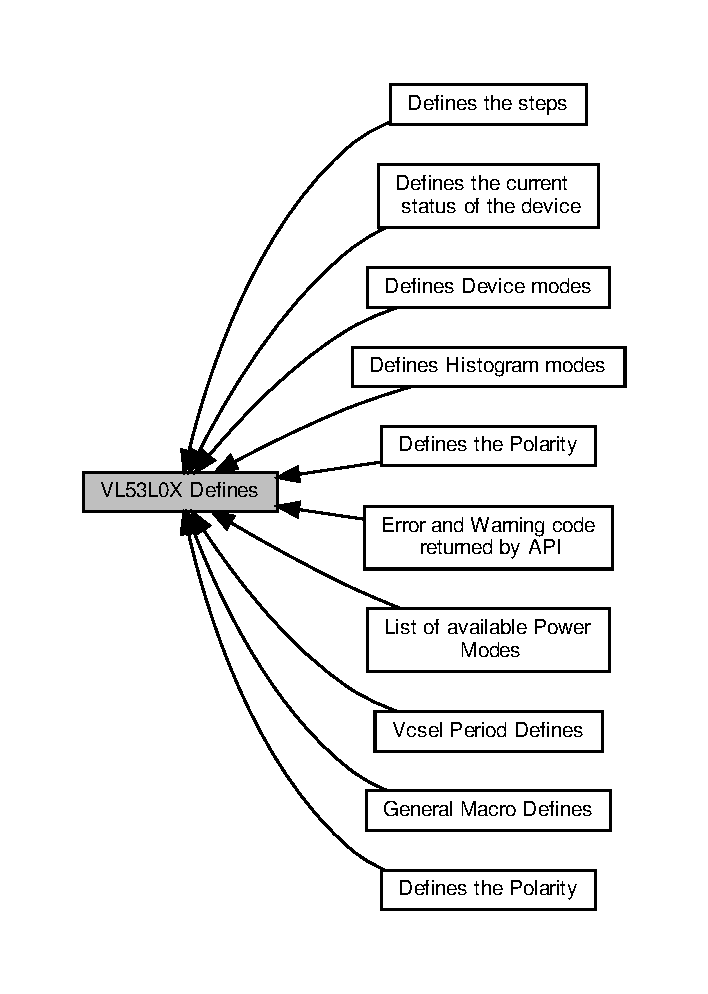
\includegraphics[width=340pt]{group__VL53L0X__globaldefine__group}
\end{center}
\end{figure}
\subsection*{Modules}
\begin{DoxyCompactItemize}
\item 
\hyperlink{group__VL53L0X__define__Error__group}{Error and Warning code returned by A\+PI}
\item 
\hyperlink{group__VL53L0X__define__DeviceModes__group}{Defines Device modes}
\item 
\hyperlink{group__VL53L0X__define__HistogramModes__group}{Defines Histogram modes}
\item 
\hyperlink{group__VL53L0X__define__PowerModes__group}{List of available Power Modes}
\item 
\hyperlink{group__VL53L0X__define__State__group}{Defines the current status of the device}
\item 
\hyperlink{group__VL53L0X__define__InterruptPolarity__group}{Defines the Polarity}
\item 
\hyperlink{group__VL53L0X__define__VcselPeriod__group}{Vcsel Period Defines}
\item 
\hyperlink{group__VL53L0X__define__SchedulerSequence__group}{Defines the steps}
\item 
\hyperlink{group__VL53L0X__define__SequenceStepId__group}{Defines the Polarity}
\item 
\hyperlink{group__VL53L0X__define__GeneralMacro__group}{General Macro Defines}
\end{DoxyCompactItemize}
\subsection*{Classes}
\begin{DoxyCompactItemize}
\item 
struct \hyperlink{structVL53L0X__Version__t}{V\+L53\+L0\+X\+\_\+\+Version\+\_\+t}
\begin{DoxyCompactList}\small\item\em Defines the parameters of the Get Version Functions. \end{DoxyCompactList}\item 
struct \hyperlink{structVL53L0X__DeviceInfo__t}{V\+L53\+L0\+X\+\_\+\+Device\+Info\+\_\+t}
\begin{DoxyCompactList}\small\item\em Defines the parameters of the Get Device Info Functions. \end{DoxyCompactList}\item 
struct \hyperlink{structVL53L0X__DeviceParameters__t}{V\+L53\+L0\+X\+\_\+\+Device\+Parameters\+\_\+t}
\begin{DoxyCompactList}\small\item\em Defines all parameters for the device. \end{DoxyCompactList}\item 
struct \hyperlink{structVL53L0X__DMaxData__t}{V\+L53\+L0\+X\+\_\+\+D\+Max\+Data\+\_\+t}
\begin{DoxyCompactList}\small\item\em \hyperlink{structStructure}{Structure} containing the Dmax computation parameters and data. \end{DoxyCompactList}\item 
struct \hyperlink{structVL53L0X__RangingMeasurementData__t}{V\+L53\+L0\+X\+\_\+\+Ranging\+Measurement\+Data\+\_\+t}
\item 
struct \hyperlink{structVL53L0X__HistogramMeasurementData__t}{V\+L53\+L0\+X\+\_\+\+Histogram\+Measurement\+Data\+\_\+t}
\item 
struct \hyperlink{structVL53L0X__SpadData__t}{V\+L53\+L0\+X\+\_\+\+Spad\+Data\+\_\+t}
\begin{DoxyCompactList}\small\item\em Spad Configuration Data. \end{DoxyCompactList}\item 
struct \hyperlink{structVL53L0X__DeviceSpecificParameters__t}{V\+L53\+L0\+X\+\_\+\+Device\+Specific\+Parameters\+\_\+t}
\item 
struct \hyperlink{structVL53L0X__DevData__t}{V\+L53\+L0\+X\+\_\+\+Dev\+Data\+\_\+t}
\begin{DoxyCompactList}\small\item\em V\+L53\+L0X P\+AL device ST private data structure ~\newline
End user should never access any of these field directly. \end{DoxyCompactList}\item 
struct \hyperlink{structVL53L0X__RangeData__t}{V\+L53\+L0\+X\+\_\+\+Range\+Data\+\_\+t}
\begin{DoxyCompactList}\small\item\em Range measurement data. \end{DoxyCompactList}\item 
struct \hyperlink{structVL53L0X__HistogramData__t}{V\+L53\+L0\+X\+\_\+\+Histogram\+Data\+\_\+t}
\begin{DoxyCompactList}\small\item\em Histogram measurement data. \end{DoxyCompactList}\end{DoxyCompactItemize}
\subsection*{Macros}
\begin{DoxyCompactItemize}
\item 
\#define \hyperlink{group__VL53L0X__globaldefine__group_ga4436dba3d980a0aa455ac8d349d0548f}{V\+L53\+L0\+X10\+\_\+\+S\+P\+E\+C\+I\+F\+I\+C\+A\+T\+I\+O\+N\+\_\+\+V\+E\+R\+\_\+\+M\+A\+J\+OR}~1
\item 
\#define \hyperlink{group__VL53L0X__globaldefine__group_ga165ca09869a75a47af2c86dded92b2ff}{V\+L53\+L0\+X10\+\_\+\+S\+P\+E\+C\+I\+F\+I\+C\+A\+T\+I\+O\+N\+\_\+\+V\+E\+R\+\_\+\+M\+I\+N\+OR}~2
\item 
\#define \hyperlink{group__VL53L0X__globaldefine__group_gafcd69daf7d710455aa2f8125fb344b01}{V\+L53\+L0\+X10\+\_\+\+S\+P\+E\+C\+I\+F\+I\+C\+A\+T\+I\+O\+N\+\_\+\+V\+E\+R\+\_\+\+S\+UB}~7
\item 
\#define \hyperlink{group__VL53L0X__globaldefine__group_gaea570701997c26f8b7a52ba087f30478}{V\+L53\+L0\+X10\+\_\+\+S\+P\+E\+C\+I\+F\+I\+C\+A\+T\+I\+O\+N\+\_\+\+V\+E\+R\+\_\+\+R\+E\+V\+I\+S\+I\+ON}~1440
\item 
\#define \hyperlink{group__VL53L0X__globaldefine__group_ga00b3a9035c263c946cd344a005806e92}{V\+L53\+L0\+X10\+\_\+\+I\+M\+P\+L\+E\+M\+E\+N\+T\+A\+T\+I\+O\+N\+\_\+\+V\+E\+R\+\_\+\+M\+A\+J\+OR}~1
\item 
\#define \hyperlink{group__VL53L0X__globaldefine__group_ga4c31059c86c862f2b04033b8697e3bed}{V\+L53\+L0\+X10\+\_\+\+I\+M\+P\+L\+E\+M\+E\+N\+T\+A\+T\+I\+O\+N\+\_\+\+V\+E\+R\+\_\+\+M\+I\+N\+OR}~0
\item 
\#define \hyperlink{group__VL53L0X__globaldefine__group_gac50191a106c06fb02b9bc6b2649e8849}{V\+L53\+L0\+X10\+\_\+\+I\+M\+P\+L\+E\+M\+E\+N\+T\+A\+T\+I\+O\+N\+\_\+\+V\+E\+R\+\_\+\+S\+UB}~9
\item 
\#define \hyperlink{group__VL53L0X__globaldefine__group_gab2794b874c1d325aa4ab8594a0ec9229}{V\+L53\+L0\+X10\+\_\+\+I\+M\+P\+L\+E\+M\+E\+N\+T\+A\+T\+I\+O\+N\+\_\+\+V\+E\+R\+\_\+\+R\+E\+V\+I\+S\+I\+ON}~3673
\item 
\#define \hyperlink{group__VL53L0X__globaldefine__group_ga95f0ac7233e5b18464f683bc55684094}{V\+L53\+L0\+X\+\_\+\+S\+P\+E\+C\+I\+F\+I\+C\+A\+T\+I\+O\+N\+\_\+\+V\+E\+R\+\_\+\+M\+A\+J\+OR}~1
\item 
\#define \hyperlink{group__VL53L0X__globaldefine__group_ga5000c528311a08322528b02f6d96fec3}{V\+L53\+L0\+X\+\_\+\+S\+P\+E\+C\+I\+F\+I\+C\+A\+T\+I\+O\+N\+\_\+\+V\+E\+R\+\_\+\+M\+I\+N\+OR}~2
\item 
\#define \hyperlink{group__VL53L0X__globaldefine__group_gaf6386b67c7b174b39ffb68c97e371a4f}{V\+L53\+L0\+X\+\_\+\+S\+P\+E\+C\+I\+F\+I\+C\+A\+T\+I\+O\+N\+\_\+\+V\+E\+R\+\_\+\+S\+UB}~7
\item 
\#define \hyperlink{group__VL53L0X__globaldefine__group_gaf8da4c7bb6e36844ffac32e0dc02f929}{V\+L53\+L0\+X\+\_\+\+S\+P\+E\+C\+I\+F\+I\+C\+A\+T\+I\+O\+N\+\_\+\+V\+E\+R\+\_\+\+R\+E\+V\+I\+S\+I\+ON}~1440
\item 
\#define \hyperlink{group__VL53L0X__globaldefine__group_gae98af2f9a5d62382e35dc9cc04db28c1}{V\+L53\+L0\+X\+\_\+\+I\+M\+P\+L\+E\+M\+E\+N\+T\+A\+T\+I\+O\+N\+\_\+\+V\+E\+R\+\_\+\+M\+A\+J\+OR}~1
\item 
\#define \hyperlink{group__VL53L0X__globaldefine__group_ga27193fd4f684caa783696f1dfbdb274c}{V\+L53\+L0\+X\+\_\+\+I\+M\+P\+L\+E\+M\+E\+N\+T\+A\+T\+I\+O\+N\+\_\+\+V\+E\+R\+\_\+\+M\+I\+N\+OR}~0
\item 
\#define \hyperlink{group__VL53L0X__globaldefine__group_gab4609670434b3de664cd2863c2972ee0}{V\+L53\+L0\+X\+\_\+\+I\+M\+P\+L\+E\+M\+E\+N\+T\+A\+T\+I\+O\+N\+\_\+\+V\+E\+R\+\_\+\+S\+UB}~2
\item 
\#define \hyperlink{group__VL53L0X__globaldefine__group_gaefe0941fd2057ce01ace9f01e3b271b0}{V\+L53\+L0\+X\+\_\+\+I\+M\+P\+L\+E\+M\+E\+N\+T\+A\+T\+I\+O\+N\+\_\+\+V\+E\+R\+\_\+\+R\+E\+V\+I\+S\+I\+ON}~4823
\item 
\mbox{\Hypertarget{group__VL53L0X__globaldefine__group_ga5ea7e1c7019656a4041a4a17071a685a}\label{group__VL53L0X__globaldefine__group_ga5ea7e1c7019656a4041a4a17071a685a}} 
\#define {\bfseries V\+L53\+L0\+X\+\_\+\+D\+E\+F\+A\+U\+L\+T\+\_\+\+M\+A\+X\+\_\+\+L\+O\+OP}~2000
\item 
\mbox{\Hypertarget{group__VL53L0X__globaldefine__group_ga8fd4c45e3b62a100529d4805db1892a9}\label{group__VL53L0X__globaldefine__group_ga8fd4c45e3b62a100529d4805db1892a9}} 
\#define {\bfseries V\+L53\+L0\+X\+\_\+\+M\+A\+X\+\_\+\+S\+T\+R\+I\+N\+G\+\_\+\+L\+E\+N\+G\+TH}~32
\item 
\mbox{\Hypertarget{group__VL53L0X__globaldefine__group_gac1faec32125735bb990cd71ef0ab2637}\label{group__VL53L0X__globaldefine__group_gac1faec32125735bb990cd71ef0ab2637}} 
\#define {\bfseries V\+L53\+L0\+X\+\_\+\+H\+I\+S\+T\+O\+G\+R\+A\+M\+\_\+\+B\+U\+F\+F\+E\+R\+\_\+\+S\+I\+ZE}~24
\item 
\mbox{\Hypertarget{group__VL53L0X__globaldefine__group_gae76d61f0f709f353ddc2a811f6abf296}\label{group__VL53L0X__globaldefine__group_gae76d61f0f709f353ddc2a811f6abf296}} 
\#define {\bfseries V\+L53\+L0\+X\+\_\+\+R\+E\+F\+\_\+\+S\+P\+A\+D\+\_\+\+B\+U\+F\+F\+E\+R\+\_\+\+S\+I\+ZE}~6
\end{DoxyCompactItemize}


\subsection{Detailed Description}
V\+L53\+L0X Defines. 



\subsection{Macro Definition Documentation}
\mbox{\Hypertarget{group__VL53L0X__globaldefine__group_ga00b3a9035c263c946cd344a005806e92}\label{group__VL53L0X__globaldefine__group_ga00b3a9035c263c946cd344a005806e92}} 
\index{V\+L53\+L0\+X Defines@{V\+L53\+L0\+X Defines}!V\+L53\+L0\+X10\+\_\+\+I\+M\+P\+L\+E\+M\+E\+N\+T\+A\+T\+I\+O\+N\+\_\+\+V\+E\+R\+\_\+\+M\+A\+J\+OR@{V\+L53\+L0\+X10\+\_\+\+I\+M\+P\+L\+E\+M\+E\+N\+T\+A\+T\+I\+O\+N\+\_\+\+V\+E\+R\+\_\+\+M\+A\+J\+OR}}
\index{V\+L53\+L0\+X10\+\_\+\+I\+M\+P\+L\+E\+M\+E\+N\+T\+A\+T\+I\+O\+N\+\_\+\+V\+E\+R\+\_\+\+M\+A\+J\+OR@{V\+L53\+L0\+X10\+\_\+\+I\+M\+P\+L\+E\+M\+E\+N\+T\+A\+T\+I\+O\+N\+\_\+\+V\+E\+R\+\_\+\+M\+A\+J\+OR}!V\+L53\+L0\+X Defines@{V\+L53\+L0\+X Defines}}
\subsubsection{\texorpdfstring{V\+L53\+L0\+X10\+\_\+\+I\+M\+P\+L\+E\+M\+E\+N\+T\+A\+T\+I\+O\+N\+\_\+\+V\+E\+R\+\_\+\+M\+A\+J\+OR}{VL53L0X10\_IMPLEMENTATION\_VER\_MAJOR}}
{\footnotesize\ttfamily \#define V\+L53\+L0\+X10\+\_\+\+I\+M\+P\+L\+E\+M\+E\+N\+T\+A\+T\+I\+O\+N\+\_\+\+V\+E\+R\+\_\+\+M\+A\+J\+OR~1}

V\+L53\+L0X P\+AL I\+M\+P\+L\+E\+M\+E\+N\+T\+A\+T\+I\+ON major version \mbox{\Hypertarget{group__VL53L0X__globaldefine__group_ga4c31059c86c862f2b04033b8697e3bed}\label{group__VL53L0X__globaldefine__group_ga4c31059c86c862f2b04033b8697e3bed}} 
\index{V\+L53\+L0\+X Defines@{V\+L53\+L0\+X Defines}!V\+L53\+L0\+X10\+\_\+\+I\+M\+P\+L\+E\+M\+E\+N\+T\+A\+T\+I\+O\+N\+\_\+\+V\+E\+R\+\_\+\+M\+I\+N\+OR@{V\+L53\+L0\+X10\+\_\+\+I\+M\+P\+L\+E\+M\+E\+N\+T\+A\+T\+I\+O\+N\+\_\+\+V\+E\+R\+\_\+\+M\+I\+N\+OR}}
\index{V\+L53\+L0\+X10\+\_\+\+I\+M\+P\+L\+E\+M\+E\+N\+T\+A\+T\+I\+O\+N\+\_\+\+V\+E\+R\+\_\+\+M\+I\+N\+OR@{V\+L53\+L0\+X10\+\_\+\+I\+M\+P\+L\+E\+M\+E\+N\+T\+A\+T\+I\+O\+N\+\_\+\+V\+E\+R\+\_\+\+M\+I\+N\+OR}!V\+L53\+L0\+X Defines@{V\+L53\+L0\+X Defines}}
\subsubsection{\texorpdfstring{V\+L53\+L0\+X10\+\_\+\+I\+M\+P\+L\+E\+M\+E\+N\+T\+A\+T\+I\+O\+N\+\_\+\+V\+E\+R\+\_\+\+M\+I\+N\+OR}{VL53L0X10\_IMPLEMENTATION\_VER\_MINOR}}
{\footnotesize\ttfamily \#define V\+L53\+L0\+X10\+\_\+\+I\+M\+P\+L\+E\+M\+E\+N\+T\+A\+T\+I\+O\+N\+\_\+\+V\+E\+R\+\_\+\+M\+I\+N\+OR~0}

V\+L53\+L0X P\+AL I\+M\+P\+L\+E\+M\+E\+N\+T\+A\+T\+I\+ON minor version \mbox{\Hypertarget{group__VL53L0X__globaldefine__group_gab2794b874c1d325aa4ab8594a0ec9229}\label{group__VL53L0X__globaldefine__group_gab2794b874c1d325aa4ab8594a0ec9229}} 
\index{V\+L53\+L0\+X Defines@{V\+L53\+L0\+X Defines}!V\+L53\+L0\+X10\+\_\+\+I\+M\+P\+L\+E\+M\+E\+N\+T\+A\+T\+I\+O\+N\+\_\+\+V\+E\+R\+\_\+\+R\+E\+V\+I\+S\+I\+ON@{V\+L53\+L0\+X10\+\_\+\+I\+M\+P\+L\+E\+M\+E\+N\+T\+A\+T\+I\+O\+N\+\_\+\+V\+E\+R\+\_\+\+R\+E\+V\+I\+S\+I\+ON}}
\index{V\+L53\+L0\+X10\+\_\+\+I\+M\+P\+L\+E\+M\+E\+N\+T\+A\+T\+I\+O\+N\+\_\+\+V\+E\+R\+\_\+\+R\+E\+V\+I\+S\+I\+ON@{V\+L53\+L0\+X10\+\_\+\+I\+M\+P\+L\+E\+M\+E\+N\+T\+A\+T\+I\+O\+N\+\_\+\+V\+E\+R\+\_\+\+R\+E\+V\+I\+S\+I\+ON}!V\+L53\+L0\+X Defines@{V\+L53\+L0\+X Defines}}
\subsubsection{\texorpdfstring{V\+L53\+L0\+X10\+\_\+\+I\+M\+P\+L\+E\+M\+E\+N\+T\+A\+T\+I\+O\+N\+\_\+\+V\+E\+R\+\_\+\+R\+E\+V\+I\+S\+I\+ON}{VL53L0X10\_IMPLEMENTATION\_VER\_REVISION}}
{\footnotesize\ttfamily \#define V\+L53\+L0\+X10\+\_\+\+I\+M\+P\+L\+E\+M\+E\+N\+T\+A\+T\+I\+O\+N\+\_\+\+V\+E\+R\+\_\+\+R\+E\+V\+I\+S\+I\+ON~3673}

V\+L53\+L0X P\+AL I\+M\+P\+L\+E\+M\+E\+N\+T\+A\+T\+I\+ON sub version \mbox{\Hypertarget{group__VL53L0X__globaldefine__group_gac50191a106c06fb02b9bc6b2649e8849}\label{group__VL53L0X__globaldefine__group_gac50191a106c06fb02b9bc6b2649e8849}} 
\index{V\+L53\+L0\+X Defines@{V\+L53\+L0\+X Defines}!V\+L53\+L0\+X10\+\_\+\+I\+M\+P\+L\+E\+M\+E\+N\+T\+A\+T\+I\+O\+N\+\_\+\+V\+E\+R\+\_\+\+S\+UB@{V\+L53\+L0\+X10\+\_\+\+I\+M\+P\+L\+E\+M\+E\+N\+T\+A\+T\+I\+O\+N\+\_\+\+V\+E\+R\+\_\+\+S\+UB}}
\index{V\+L53\+L0\+X10\+\_\+\+I\+M\+P\+L\+E\+M\+E\+N\+T\+A\+T\+I\+O\+N\+\_\+\+V\+E\+R\+\_\+\+S\+UB@{V\+L53\+L0\+X10\+\_\+\+I\+M\+P\+L\+E\+M\+E\+N\+T\+A\+T\+I\+O\+N\+\_\+\+V\+E\+R\+\_\+\+S\+UB}!V\+L53\+L0\+X Defines@{V\+L53\+L0\+X Defines}}
\subsubsection{\texorpdfstring{V\+L53\+L0\+X10\+\_\+\+I\+M\+P\+L\+E\+M\+E\+N\+T\+A\+T\+I\+O\+N\+\_\+\+V\+E\+R\+\_\+\+S\+UB}{VL53L0X10\_IMPLEMENTATION\_VER\_SUB}}
{\footnotesize\ttfamily \#define V\+L53\+L0\+X10\+\_\+\+I\+M\+P\+L\+E\+M\+E\+N\+T\+A\+T\+I\+O\+N\+\_\+\+V\+E\+R\+\_\+\+S\+UB~9}

V\+L53\+L0X P\+AL I\+M\+P\+L\+E\+M\+E\+N\+T\+A\+T\+I\+ON sub version \mbox{\Hypertarget{group__VL53L0X__globaldefine__group_ga4436dba3d980a0aa455ac8d349d0548f}\label{group__VL53L0X__globaldefine__group_ga4436dba3d980a0aa455ac8d349d0548f}} 
\index{V\+L53\+L0\+X Defines@{V\+L53\+L0\+X Defines}!V\+L53\+L0\+X10\+\_\+\+S\+P\+E\+C\+I\+F\+I\+C\+A\+T\+I\+O\+N\+\_\+\+V\+E\+R\+\_\+\+M\+A\+J\+OR@{V\+L53\+L0\+X10\+\_\+\+S\+P\+E\+C\+I\+F\+I\+C\+A\+T\+I\+O\+N\+\_\+\+V\+E\+R\+\_\+\+M\+A\+J\+OR}}
\index{V\+L53\+L0\+X10\+\_\+\+S\+P\+E\+C\+I\+F\+I\+C\+A\+T\+I\+O\+N\+\_\+\+V\+E\+R\+\_\+\+M\+A\+J\+OR@{V\+L53\+L0\+X10\+\_\+\+S\+P\+E\+C\+I\+F\+I\+C\+A\+T\+I\+O\+N\+\_\+\+V\+E\+R\+\_\+\+M\+A\+J\+OR}!V\+L53\+L0\+X Defines@{V\+L53\+L0\+X Defines}}
\subsubsection{\texorpdfstring{V\+L53\+L0\+X10\+\_\+\+S\+P\+E\+C\+I\+F\+I\+C\+A\+T\+I\+O\+N\+\_\+\+V\+E\+R\+\_\+\+M\+A\+J\+OR}{VL53L0X10\_SPECIFICATION\_VER\_MAJOR}}
{\footnotesize\ttfamily \#define V\+L53\+L0\+X10\+\_\+\+S\+P\+E\+C\+I\+F\+I\+C\+A\+T\+I\+O\+N\+\_\+\+V\+E\+R\+\_\+\+M\+A\+J\+OR~1}

P\+AL S\+P\+E\+C\+I\+F\+I\+C\+A\+T\+I\+ON major version \mbox{\Hypertarget{group__VL53L0X__globaldefine__group_ga165ca09869a75a47af2c86dded92b2ff}\label{group__VL53L0X__globaldefine__group_ga165ca09869a75a47af2c86dded92b2ff}} 
\index{V\+L53\+L0\+X Defines@{V\+L53\+L0\+X Defines}!V\+L53\+L0\+X10\+\_\+\+S\+P\+E\+C\+I\+F\+I\+C\+A\+T\+I\+O\+N\+\_\+\+V\+E\+R\+\_\+\+M\+I\+N\+OR@{V\+L53\+L0\+X10\+\_\+\+S\+P\+E\+C\+I\+F\+I\+C\+A\+T\+I\+O\+N\+\_\+\+V\+E\+R\+\_\+\+M\+I\+N\+OR}}
\index{V\+L53\+L0\+X10\+\_\+\+S\+P\+E\+C\+I\+F\+I\+C\+A\+T\+I\+O\+N\+\_\+\+V\+E\+R\+\_\+\+M\+I\+N\+OR@{V\+L53\+L0\+X10\+\_\+\+S\+P\+E\+C\+I\+F\+I\+C\+A\+T\+I\+O\+N\+\_\+\+V\+E\+R\+\_\+\+M\+I\+N\+OR}!V\+L53\+L0\+X Defines@{V\+L53\+L0\+X Defines}}
\subsubsection{\texorpdfstring{V\+L53\+L0\+X10\+\_\+\+S\+P\+E\+C\+I\+F\+I\+C\+A\+T\+I\+O\+N\+\_\+\+V\+E\+R\+\_\+\+M\+I\+N\+OR}{VL53L0X10\_SPECIFICATION\_VER\_MINOR}}
{\footnotesize\ttfamily \#define V\+L53\+L0\+X10\+\_\+\+S\+P\+E\+C\+I\+F\+I\+C\+A\+T\+I\+O\+N\+\_\+\+V\+E\+R\+\_\+\+M\+I\+N\+OR~2}

P\+AL S\+P\+E\+C\+I\+F\+I\+C\+A\+T\+I\+ON minor version \mbox{\Hypertarget{group__VL53L0X__globaldefine__group_gaea570701997c26f8b7a52ba087f30478}\label{group__VL53L0X__globaldefine__group_gaea570701997c26f8b7a52ba087f30478}} 
\index{V\+L53\+L0\+X Defines@{V\+L53\+L0\+X Defines}!V\+L53\+L0\+X10\+\_\+\+S\+P\+E\+C\+I\+F\+I\+C\+A\+T\+I\+O\+N\+\_\+\+V\+E\+R\+\_\+\+R\+E\+V\+I\+S\+I\+ON@{V\+L53\+L0\+X10\+\_\+\+S\+P\+E\+C\+I\+F\+I\+C\+A\+T\+I\+O\+N\+\_\+\+V\+E\+R\+\_\+\+R\+E\+V\+I\+S\+I\+ON}}
\index{V\+L53\+L0\+X10\+\_\+\+S\+P\+E\+C\+I\+F\+I\+C\+A\+T\+I\+O\+N\+\_\+\+V\+E\+R\+\_\+\+R\+E\+V\+I\+S\+I\+ON@{V\+L53\+L0\+X10\+\_\+\+S\+P\+E\+C\+I\+F\+I\+C\+A\+T\+I\+O\+N\+\_\+\+V\+E\+R\+\_\+\+R\+E\+V\+I\+S\+I\+ON}!V\+L53\+L0\+X Defines@{V\+L53\+L0\+X Defines}}
\subsubsection{\texorpdfstring{V\+L53\+L0\+X10\+\_\+\+S\+P\+E\+C\+I\+F\+I\+C\+A\+T\+I\+O\+N\+\_\+\+V\+E\+R\+\_\+\+R\+E\+V\+I\+S\+I\+ON}{VL53L0X10\_SPECIFICATION\_VER\_REVISION}}
{\footnotesize\ttfamily \#define V\+L53\+L0\+X10\+\_\+\+S\+P\+E\+C\+I\+F\+I\+C\+A\+T\+I\+O\+N\+\_\+\+V\+E\+R\+\_\+\+R\+E\+V\+I\+S\+I\+ON~1440}

P\+AL S\+P\+E\+C\+I\+F\+I\+C\+A\+T\+I\+ON sub version \mbox{\Hypertarget{group__VL53L0X__globaldefine__group_gafcd69daf7d710455aa2f8125fb344b01}\label{group__VL53L0X__globaldefine__group_gafcd69daf7d710455aa2f8125fb344b01}} 
\index{V\+L53\+L0\+X Defines@{V\+L53\+L0\+X Defines}!V\+L53\+L0\+X10\+\_\+\+S\+P\+E\+C\+I\+F\+I\+C\+A\+T\+I\+O\+N\+\_\+\+V\+E\+R\+\_\+\+S\+UB@{V\+L53\+L0\+X10\+\_\+\+S\+P\+E\+C\+I\+F\+I\+C\+A\+T\+I\+O\+N\+\_\+\+V\+E\+R\+\_\+\+S\+UB}}
\index{V\+L53\+L0\+X10\+\_\+\+S\+P\+E\+C\+I\+F\+I\+C\+A\+T\+I\+O\+N\+\_\+\+V\+E\+R\+\_\+\+S\+UB@{V\+L53\+L0\+X10\+\_\+\+S\+P\+E\+C\+I\+F\+I\+C\+A\+T\+I\+O\+N\+\_\+\+V\+E\+R\+\_\+\+S\+UB}!V\+L53\+L0\+X Defines@{V\+L53\+L0\+X Defines}}
\subsubsection{\texorpdfstring{V\+L53\+L0\+X10\+\_\+\+S\+P\+E\+C\+I\+F\+I\+C\+A\+T\+I\+O\+N\+\_\+\+V\+E\+R\+\_\+\+S\+UB}{VL53L0X10\_SPECIFICATION\_VER\_SUB}}
{\footnotesize\ttfamily \#define V\+L53\+L0\+X10\+\_\+\+S\+P\+E\+C\+I\+F\+I\+C\+A\+T\+I\+O\+N\+\_\+\+V\+E\+R\+\_\+\+S\+UB~7}

P\+AL S\+P\+E\+C\+I\+F\+I\+C\+A\+T\+I\+ON sub version \mbox{\Hypertarget{group__VL53L0X__globaldefine__group_gae98af2f9a5d62382e35dc9cc04db28c1}\label{group__VL53L0X__globaldefine__group_gae98af2f9a5d62382e35dc9cc04db28c1}} 
\index{V\+L53\+L0\+X Defines@{V\+L53\+L0\+X Defines}!V\+L53\+L0\+X\+\_\+\+I\+M\+P\+L\+E\+M\+E\+N\+T\+A\+T\+I\+O\+N\+\_\+\+V\+E\+R\+\_\+\+M\+A\+J\+OR@{V\+L53\+L0\+X\+\_\+\+I\+M\+P\+L\+E\+M\+E\+N\+T\+A\+T\+I\+O\+N\+\_\+\+V\+E\+R\+\_\+\+M\+A\+J\+OR}}
\index{V\+L53\+L0\+X\+\_\+\+I\+M\+P\+L\+E\+M\+E\+N\+T\+A\+T\+I\+O\+N\+\_\+\+V\+E\+R\+\_\+\+M\+A\+J\+OR@{V\+L53\+L0\+X\+\_\+\+I\+M\+P\+L\+E\+M\+E\+N\+T\+A\+T\+I\+O\+N\+\_\+\+V\+E\+R\+\_\+\+M\+A\+J\+OR}!V\+L53\+L0\+X Defines@{V\+L53\+L0\+X Defines}}
\subsubsection{\texorpdfstring{V\+L53\+L0\+X\+\_\+\+I\+M\+P\+L\+E\+M\+E\+N\+T\+A\+T\+I\+O\+N\+\_\+\+V\+E\+R\+\_\+\+M\+A\+J\+OR}{VL53L0X\_IMPLEMENTATION\_VER\_MAJOR}}
{\footnotesize\ttfamily \#define V\+L53\+L0\+X\+\_\+\+I\+M\+P\+L\+E\+M\+E\+N\+T\+A\+T\+I\+O\+N\+\_\+\+V\+E\+R\+\_\+\+M\+A\+J\+OR~1}

V\+L53\+L0X P\+AL I\+M\+P\+L\+E\+M\+E\+N\+T\+A\+T\+I\+ON major version \mbox{\Hypertarget{group__VL53L0X__globaldefine__group_ga27193fd4f684caa783696f1dfbdb274c}\label{group__VL53L0X__globaldefine__group_ga27193fd4f684caa783696f1dfbdb274c}} 
\index{V\+L53\+L0\+X Defines@{V\+L53\+L0\+X Defines}!V\+L53\+L0\+X\+\_\+\+I\+M\+P\+L\+E\+M\+E\+N\+T\+A\+T\+I\+O\+N\+\_\+\+V\+E\+R\+\_\+\+M\+I\+N\+OR@{V\+L53\+L0\+X\+\_\+\+I\+M\+P\+L\+E\+M\+E\+N\+T\+A\+T\+I\+O\+N\+\_\+\+V\+E\+R\+\_\+\+M\+I\+N\+OR}}
\index{V\+L53\+L0\+X\+\_\+\+I\+M\+P\+L\+E\+M\+E\+N\+T\+A\+T\+I\+O\+N\+\_\+\+V\+E\+R\+\_\+\+M\+I\+N\+OR@{V\+L53\+L0\+X\+\_\+\+I\+M\+P\+L\+E\+M\+E\+N\+T\+A\+T\+I\+O\+N\+\_\+\+V\+E\+R\+\_\+\+M\+I\+N\+OR}!V\+L53\+L0\+X Defines@{V\+L53\+L0\+X Defines}}
\subsubsection{\texorpdfstring{V\+L53\+L0\+X\+\_\+\+I\+M\+P\+L\+E\+M\+E\+N\+T\+A\+T\+I\+O\+N\+\_\+\+V\+E\+R\+\_\+\+M\+I\+N\+OR}{VL53L0X\_IMPLEMENTATION\_VER\_MINOR}}
{\footnotesize\ttfamily \#define V\+L53\+L0\+X\+\_\+\+I\+M\+P\+L\+E\+M\+E\+N\+T\+A\+T\+I\+O\+N\+\_\+\+V\+E\+R\+\_\+\+M\+I\+N\+OR~0}

V\+L53\+L0X P\+AL I\+M\+P\+L\+E\+M\+E\+N\+T\+A\+T\+I\+ON minor version \mbox{\Hypertarget{group__VL53L0X__globaldefine__group_gaefe0941fd2057ce01ace9f01e3b271b0}\label{group__VL53L0X__globaldefine__group_gaefe0941fd2057ce01ace9f01e3b271b0}} 
\index{V\+L53\+L0\+X Defines@{V\+L53\+L0\+X Defines}!V\+L53\+L0\+X\+\_\+\+I\+M\+P\+L\+E\+M\+E\+N\+T\+A\+T\+I\+O\+N\+\_\+\+V\+E\+R\+\_\+\+R\+E\+V\+I\+S\+I\+ON@{V\+L53\+L0\+X\+\_\+\+I\+M\+P\+L\+E\+M\+E\+N\+T\+A\+T\+I\+O\+N\+\_\+\+V\+E\+R\+\_\+\+R\+E\+V\+I\+S\+I\+ON}}
\index{V\+L53\+L0\+X\+\_\+\+I\+M\+P\+L\+E\+M\+E\+N\+T\+A\+T\+I\+O\+N\+\_\+\+V\+E\+R\+\_\+\+R\+E\+V\+I\+S\+I\+ON@{V\+L53\+L0\+X\+\_\+\+I\+M\+P\+L\+E\+M\+E\+N\+T\+A\+T\+I\+O\+N\+\_\+\+V\+E\+R\+\_\+\+R\+E\+V\+I\+S\+I\+ON}!V\+L53\+L0\+X Defines@{V\+L53\+L0\+X Defines}}
\subsubsection{\texorpdfstring{V\+L53\+L0\+X\+\_\+\+I\+M\+P\+L\+E\+M\+E\+N\+T\+A\+T\+I\+O\+N\+\_\+\+V\+E\+R\+\_\+\+R\+E\+V\+I\+S\+I\+ON}{VL53L0X\_IMPLEMENTATION\_VER\_REVISION}}
{\footnotesize\ttfamily \#define V\+L53\+L0\+X\+\_\+\+I\+M\+P\+L\+E\+M\+E\+N\+T\+A\+T\+I\+O\+N\+\_\+\+V\+E\+R\+\_\+\+R\+E\+V\+I\+S\+I\+ON~4823}

V\+L53\+L0X P\+AL I\+M\+P\+L\+E\+M\+E\+N\+T\+A\+T\+I\+ON sub version \mbox{\Hypertarget{group__VL53L0X__globaldefine__group_gab4609670434b3de664cd2863c2972ee0}\label{group__VL53L0X__globaldefine__group_gab4609670434b3de664cd2863c2972ee0}} 
\index{V\+L53\+L0\+X Defines@{V\+L53\+L0\+X Defines}!V\+L53\+L0\+X\+\_\+\+I\+M\+P\+L\+E\+M\+E\+N\+T\+A\+T\+I\+O\+N\+\_\+\+V\+E\+R\+\_\+\+S\+UB@{V\+L53\+L0\+X\+\_\+\+I\+M\+P\+L\+E\+M\+E\+N\+T\+A\+T\+I\+O\+N\+\_\+\+V\+E\+R\+\_\+\+S\+UB}}
\index{V\+L53\+L0\+X\+\_\+\+I\+M\+P\+L\+E\+M\+E\+N\+T\+A\+T\+I\+O\+N\+\_\+\+V\+E\+R\+\_\+\+S\+UB@{V\+L53\+L0\+X\+\_\+\+I\+M\+P\+L\+E\+M\+E\+N\+T\+A\+T\+I\+O\+N\+\_\+\+V\+E\+R\+\_\+\+S\+UB}!V\+L53\+L0\+X Defines@{V\+L53\+L0\+X Defines}}
\subsubsection{\texorpdfstring{V\+L53\+L0\+X\+\_\+\+I\+M\+P\+L\+E\+M\+E\+N\+T\+A\+T\+I\+O\+N\+\_\+\+V\+E\+R\+\_\+\+S\+UB}{VL53L0X\_IMPLEMENTATION\_VER\_SUB}}
{\footnotesize\ttfamily \#define V\+L53\+L0\+X\+\_\+\+I\+M\+P\+L\+E\+M\+E\+N\+T\+A\+T\+I\+O\+N\+\_\+\+V\+E\+R\+\_\+\+S\+UB~2}

V\+L53\+L0X P\+AL I\+M\+P\+L\+E\+M\+E\+N\+T\+A\+T\+I\+ON sub version \mbox{\Hypertarget{group__VL53L0X__globaldefine__group_ga95f0ac7233e5b18464f683bc55684094}\label{group__VL53L0X__globaldefine__group_ga95f0ac7233e5b18464f683bc55684094}} 
\index{V\+L53\+L0\+X Defines@{V\+L53\+L0\+X Defines}!V\+L53\+L0\+X\+\_\+\+S\+P\+E\+C\+I\+F\+I\+C\+A\+T\+I\+O\+N\+\_\+\+V\+E\+R\+\_\+\+M\+A\+J\+OR@{V\+L53\+L0\+X\+\_\+\+S\+P\+E\+C\+I\+F\+I\+C\+A\+T\+I\+O\+N\+\_\+\+V\+E\+R\+\_\+\+M\+A\+J\+OR}}
\index{V\+L53\+L0\+X\+\_\+\+S\+P\+E\+C\+I\+F\+I\+C\+A\+T\+I\+O\+N\+\_\+\+V\+E\+R\+\_\+\+M\+A\+J\+OR@{V\+L53\+L0\+X\+\_\+\+S\+P\+E\+C\+I\+F\+I\+C\+A\+T\+I\+O\+N\+\_\+\+V\+E\+R\+\_\+\+M\+A\+J\+OR}!V\+L53\+L0\+X Defines@{V\+L53\+L0\+X Defines}}
\subsubsection{\texorpdfstring{V\+L53\+L0\+X\+\_\+\+S\+P\+E\+C\+I\+F\+I\+C\+A\+T\+I\+O\+N\+\_\+\+V\+E\+R\+\_\+\+M\+A\+J\+OR}{VL53L0X\_SPECIFICATION\_VER\_MAJOR}}
{\footnotesize\ttfamily \#define V\+L53\+L0\+X\+\_\+\+S\+P\+E\+C\+I\+F\+I\+C\+A\+T\+I\+O\+N\+\_\+\+V\+E\+R\+\_\+\+M\+A\+J\+OR~1}

P\+AL S\+P\+E\+C\+I\+F\+I\+C\+A\+T\+I\+ON major version \mbox{\Hypertarget{group__VL53L0X__globaldefine__group_ga5000c528311a08322528b02f6d96fec3}\label{group__VL53L0X__globaldefine__group_ga5000c528311a08322528b02f6d96fec3}} 
\index{V\+L53\+L0\+X Defines@{V\+L53\+L0\+X Defines}!V\+L53\+L0\+X\+\_\+\+S\+P\+E\+C\+I\+F\+I\+C\+A\+T\+I\+O\+N\+\_\+\+V\+E\+R\+\_\+\+M\+I\+N\+OR@{V\+L53\+L0\+X\+\_\+\+S\+P\+E\+C\+I\+F\+I\+C\+A\+T\+I\+O\+N\+\_\+\+V\+E\+R\+\_\+\+M\+I\+N\+OR}}
\index{V\+L53\+L0\+X\+\_\+\+S\+P\+E\+C\+I\+F\+I\+C\+A\+T\+I\+O\+N\+\_\+\+V\+E\+R\+\_\+\+M\+I\+N\+OR@{V\+L53\+L0\+X\+\_\+\+S\+P\+E\+C\+I\+F\+I\+C\+A\+T\+I\+O\+N\+\_\+\+V\+E\+R\+\_\+\+M\+I\+N\+OR}!V\+L53\+L0\+X Defines@{V\+L53\+L0\+X Defines}}
\subsubsection{\texorpdfstring{V\+L53\+L0\+X\+\_\+\+S\+P\+E\+C\+I\+F\+I\+C\+A\+T\+I\+O\+N\+\_\+\+V\+E\+R\+\_\+\+M\+I\+N\+OR}{VL53L0X\_SPECIFICATION\_VER\_MINOR}}
{\footnotesize\ttfamily \#define V\+L53\+L0\+X\+\_\+\+S\+P\+E\+C\+I\+F\+I\+C\+A\+T\+I\+O\+N\+\_\+\+V\+E\+R\+\_\+\+M\+I\+N\+OR~2}

P\+AL S\+P\+E\+C\+I\+F\+I\+C\+A\+T\+I\+ON minor version \mbox{\Hypertarget{group__VL53L0X__globaldefine__group_gaf8da4c7bb6e36844ffac32e0dc02f929}\label{group__VL53L0X__globaldefine__group_gaf8da4c7bb6e36844ffac32e0dc02f929}} 
\index{V\+L53\+L0\+X Defines@{V\+L53\+L0\+X Defines}!V\+L53\+L0\+X\+\_\+\+S\+P\+E\+C\+I\+F\+I\+C\+A\+T\+I\+O\+N\+\_\+\+V\+E\+R\+\_\+\+R\+E\+V\+I\+S\+I\+ON@{V\+L53\+L0\+X\+\_\+\+S\+P\+E\+C\+I\+F\+I\+C\+A\+T\+I\+O\+N\+\_\+\+V\+E\+R\+\_\+\+R\+E\+V\+I\+S\+I\+ON}}
\index{V\+L53\+L0\+X\+\_\+\+S\+P\+E\+C\+I\+F\+I\+C\+A\+T\+I\+O\+N\+\_\+\+V\+E\+R\+\_\+\+R\+E\+V\+I\+S\+I\+ON@{V\+L53\+L0\+X\+\_\+\+S\+P\+E\+C\+I\+F\+I\+C\+A\+T\+I\+O\+N\+\_\+\+V\+E\+R\+\_\+\+R\+E\+V\+I\+S\+I\+ON}!V\+L53\+L0\+X Defines@{V\+L53\+L0\+X Defines}}
\subsubsection{\texorpdfstring{V\+L53\+L0\+X\+\_\+\+S\+P\+E\+C\+I\+F\+I\+C\+A\+T\+I\+O\+N\+\_\+\+V\+E\+R\+\_\+\+R\+E\+V\+I\+S\+I\+ON}{VL53L0X\_SPECIFICATION\_VER\_REVISION}}
{\footnotesize\ttfamily \#define V\+L53\+L0\+X\+\_\+\+S\+P\+E\+C\+I\+F\+I\+C\+A\+T\+I\+O\+N\+\_\+\+V\+E\+R\+\_\+\+R\+E\+V\+I\+S\+I\+ON~1440}

P\+AL S\+P\+E\+C\+I\+F\+I\+C\+A\+T\+I\+ON sub version \mbox{\Hypertarget{group__VL53L0X__globaldefine__group_gaf6386b67c7b174b39ffb68c97e371a4f}\label{group__VL53L0X__globaldefine__group_gaf6386b67c7b174b39ffb68c97e371a4f}} 
\index{V\+L53\+L0\+X Defines@{V\+L53\+L0\+X Defines}!V\+L53\+L0\+X\+\_\+\+S\+P\+E\+C\+I\+F\+I\+C\+A\+T\+I\+O\+N\+\_\+\+V\+E\+R\+\_\+\+S\+UB@{V\+L53\+L0\+X\+\_\+\+S\+P\+E\+C\+I\+F\+I\+C\+A\+T\+I\+O\+N\+\_\+\+V\+E\+R\+\_\+\+S\+UB}}
\index{V\+L53\+L0\+X\+\_\+\+S\+P\+E\+C\+I\+F\+I\+C\+A\+T\+I\+O\+N\+\_\+\+V\+E\+R\+\_\+\+S\+UB@{V\+L53\+L0\+X\+\_\+\+S\+P\+E\+C\+I\+F\+I\+C\+A\+T\+I\+O\+N\+\_\+\+V\+E\+R\+\_\+\+S\+UB}!V\+L53\+L0\+X Defines@{V\+L53\+L0\+X Defines}}
\subsubsection{\texorpdfstring{V\+L53\+L0\+X\+\_\+\+S\+P\+E\+C\+I\+F\+I\+C\+A\+T\+I\+O\+N\+\_\+\+V\+E\+R\+\_\+\+S\+UB}{VL53L0X\_SPECIFICATION\_VER\_SUB}}
{\footnotesize\ttfamily \#define V\+L53\+L0\+X\+\_\+\+S\+P\+E\+C\+I\+F\+I\+C\+A\+T\+I\+O\+N\+\_\+\+V\+E\+R\+\_\+\+S\+UB~7}

P\+AL S\+P\+E\+C\+I\+F\+I\+C\+A\+T\+I\+ON sub version 
\hypertarget{group__VL53L0X__define__Error__group}{}\section{Error and Warning code returned by A\+PI}
\label{group__VL53L0X__define__Error__group}\index{Error and Warning code returned by A\+PI@{Error and Warning code returned by A\+PI}}
Collaboration diagram for Error and Warning code returned by A\+PI\+:\nopagebreak
\begin{figure}[H]
\begin{center}
\leavevmode
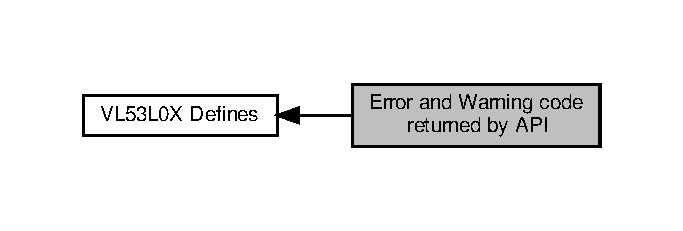
\includegraphics[width=328pt]{group__VL53L0X__define__Error__group}
\end{center}
\end{figure}
\subsection*{Macros}
\begin{DoxyCompactItemize}
\item 
\mbox{\Hypertarget{group__VL53L0X__define__Error__group_gab1bcfe4c791fa91012ccf489a260430a}\label{group__VL53L0X__define__Error__group_gab1bcfe4c791fa91012ccf489a260430a}} 
\#define {\bfseries V\+L53\+L0\+X\+\_\+\+E\+R\+R\+O\+R\+\_\+\+N\+O\+NE}~((V\+L53\+L0\+X\+\_\+\+Error)    0)
\item 
\#define \hyperlink{group__VL53L0X__define__Error__group_ga4bc7046c2d7a01b8c925af91d5325a65}{V\+L53\+L0\+X\+\_\+\+E\+R\+R\+O\+R\+\_\+\+C\+A\+L\+I\+B\+R\+A\+T\+I\+O\+N\+\_\+\+W\+A\+R\+N\+I\+NG}~((V\+L53\+L0\+X\+\_\+\+Error) -\/1)
\item 
\#define \hyperlink{group__VL53L0X__define__Error__group_gaada0c813c38a4ec7a6b75646fe26129c}{V\+L53\+L0\+X\+\_\+\+E\+R\+R\+O\+R\+\_\+\+M\+I\+N\+\_\+\+C\+L\+I\+P\+P\+ED}~((V\+L53\+L0\+X\+\_\+\+Error) -\/2)
\item 
\#define \hyperlink{group__VL53L0X__define__Error__group_ga11002b39ce656b5b10bc0a9b8806e621}{V\+L53\+L0\+X\+\_\+\+E\+R\+R\+O\+R\+\_\+\+U\+N\+D\+E\+F\+I\+N\+ED}~((V\+L53\+L0\+X\+\_\+\+Error) -\/3)
\item 
\#define \hyperlink{group__VL53L0X__define__Error__group_ga445688d58f59b8d30c1a2a535522b22b}{V\+L53\+L0\+X\+\_\+\+E\+R\+R\+O\+R\+\_\+\+I\+N\+V\+A\+L\+I\+D\+\_\+\+P\+A\+R\+A\+MS}~((V\+L53\+L0\+X\+\_\+\+Error) -\/4)
\item 
\#define \hyperlink{group__VL53L0X__define__Error__group_ga0f02dc370a804f2ab8ed226ba8f0388f}{V\+L53\+L0\+X\+\_\+\+E\+R\+R\+O\+R\+\_\+\+N\+O\+T\+\_\+\+S\+U\+P\+P\+O\+R\+T\+ED}~((V\+L53\+L0\+X\+\_\+\+Error) -\/5)
\item 
\#define \hyperlink{group__VL53L0X__define__Error__group_gafa1f517e9210b3512504ce52c4028447}{V\+L53\+L0\+X\+\_\+\+E\+R\+R\+O\+R\+\_\+\+R\+A\+N\+G\+E\+\_\+\+E\+R\+R\+OR}~((V\+L53\+L0\+X\+\_\+\+Error) -\/6)
\item 
\#define \hyperlink{group__VL53L0X__define__Error__group_gaa528340d4b96f424260552676582badc}{V\+L53\+L0\+X\+\_\+\+E\+R\+R\+O\+R\+\_\+\+T\+I\+M\+E\+\_\+\+O\+UT}~((V\+L53\+L0\+X\+\_\+\+Error) -\/7)
\item 
\#define \hyperlink{group__VL53L0X__define__Error__group_ga5aaf023be40d7fa0514abdae67d49f10}{V\+L53\+L0\+X\+\_\+\+E\+R\+R\+O\+R\+\_\+\+M\+O\+D\+E\+\_\+\+N\+O\+T\+\_\+\+S\+U\+P\+P\+O\+R\+T\+ED}~((V\+L53\+L0\+X\+\_\+\+Error) -\/8)
\item 
\#define \hyperlink{group__VL53L0X__define__Error__group_gad0318b9ad0104dc41f5a661e3a6bb4bf}{V\+L53\+L0\+X\+\_\+\+E\+R\+R\+O\+R\+\_\+\+B\+U\+F\+F\+E\+R\+\_\+\+T\+O\+O\+\_\+\+S\+M\+A\+LL}~((V\+L53\+L0\+X\+\_\+\+Error) -\/9)
\item 
\#define \hyperlink{group__VL53L0X__define__Error__group_ga4c79eeda9219432ccf8de727953f4c22}{V\+L53\+L0\+X\+\_\+\+E\+R\+R\+O\+R\+\_\+\+G\+P\+I\+O\+\_\+\+N\+O\+T\+\_\+\+E\+X\+I\+S\+T\+I\+NG}~((V\+L53\+L0\+X\+\_\+\+Error) -\/10)
\item 
\#define \hyperlink{group__VL53L0X__define__Error__group_ga9fa1d66f2d200b7d81bc76df22f661b4}{V\+L53\+L0\+X\+\_\+\+E\+R\+R\+O\+R\+\_\+\+G\+P\+I\+O\+\_\+\+F\+U\+N\+C\+T\+I\+O\+N\+A\+L\+I\+T\+Y\+\_\+\+N\+O\+T\+\_\+\+S\+U\+P\+P\+O\+R\+T\+ED}~((V\+L53\+L0\+X\+\_\+\+Error) -\/11)
\item 
\#define \hyperlink{group__VL53L0X__define__Error__group_gab5679ba3df76cb304f7ea8f8e637c818}{V\+L53\+L0\+X\+\_\+\+E\+R\+R\+O\+R\+\_\+\+I\+N\+T\+E\+R\+R\+U\+P\+T\+\_\+\+N\+O\+T\+\_\+\+C\+L\+E\+A\+R\+ED}~((V\+L53\+L0\+X\+\_\+\+Error) -\/12)
\item 
\#define \hyperlink{group__VL53L0X__define__Error__group_gab1b8ae57984f4dbbfd2a4ad33656de9f}{V\+L53\+L0\+X\+\_\+\+E\+R\+R\+O\+R\+\_\+\+C\+O\+N\+T\+R\+O\+L\+\_\+\+I\+N\+T\+E\+R\+F\+A\+CE}~((V\+L53\+L0\+X\+\_\+\+Error) -\/20)
\item 
\#define \hyperlink{group__VL53L0X__define__Error__group_gaf6f072f9026fc93f6183320081eb0aec}{V\+L53\+L0\+X\+\_\+\+E\+R\+R\+O\+R\+\_\+\+I\+N\+V\+A\+L\+I\+D\+\_\+\+C\+O\+M\+M\+A\+ND}~((V\+L53\+L0\+X\+\_\+\+Error) -\/30)
\item 
\#define \hyperlink{group__VL53L0X__define__Error__group_ga000c76b4964dea1fe556d63271a5af3c}{V\+L53\+L0\+X\+\_\+\+E\+R\+R\+O\+R\+\_\+\+D\+I\+V\+I\+S\+I\+O\+N\+\_\+\+B\+Y\+\_\+\+Z\+E\+RO}~((V\+L53\+L0\+X\+\_\+\+Error) -\/40)
\item 
\#define \hyperlink{group__VL53L0X__define__Error__group_gaa87a7958ab510c391f0f9e744871f91b}{V\+L53\+L0\+X\+\_\+\+E\+R\+R\+O\+R\+\_\+\+R\+E\+F\+\_\+\+S\+P\+A\+D\+\_\+\+I\+N\+IT}~((V\+L53\+L0\+X\+\_\+\+Error) -\/50)
\item 
\#define \hyperlink{group__VL53L0X__define__Error__group_ga46f8eb3c947b3bbcef6d15d2e05169fa}{V\+L53\+L0\+X\+\_\+\+E\+R\+R\+O\+R\+\_\+\+N\+O\+T\+\_\+\+I\+M\+P\+L\+E\+M\+E\+N\+T\+ED}~((V\+L53\+L0\+X\+\_\+\+Error) -\/99)
\end{DoxyCompactItemize}
\subsection*{Typedefs}
\begin{DoxyCompactItemize}
\item 
\mbox{\Hypertarget{group__VL53L0X__define__Error__group_ga7d66c5df3ebc4b0bde0327989c0f8b04}\label{group__VL53L0X__define__Error__group_ga7d66c5df3ebc4b0bde0327989c0f8b04}} 
typedef \hyperlink{vl53l0x__types_8h_aef44329758059c91c76d334e8fc09700}{int8\+\_\+t} {\bfseries V\+L53\+L0\+X\+\_\+\+Error}
\end{DoxyCompactItemize}


\subsection{Detailed Description}
\hyperlink{structThe}{The} following D\+E\+F\+I\+NE are used to identify the P\+AL E\+R\+R\+OR 

\subsection{Macro Definition Documentation}
\mbox{\Hypertarget{group__VL53L0X__define__Error__group_gad0318b9ad0104dc41f5a661e3a6bb4bf}\label{group__VL53L0X__define__Error__group_gad0318b9ad0104dc41f5a661e3a6bb4bf}} 
\index{Error and Warning code returned by A\+PI@{Error and Warning code returned by A\+PI}!V\+L53\+L0\+X\+\_\+\+E\+R\+R\+O\+R\+\_\+\+B\+U\+F\+F\+E\+R\+\_\+\+T\+O\+O\+\_\+\+S\+M\+A\+LL@{V\+L53\+L0\+X\+\_\+\+E\+R\+R\+O\+R\+\_\+\+B\+U\+F\+F\+E\+R\+\_\+\+T\+O\+O\+\_\+\+S\+M\+A\+LL}}
\index{V\+L53\+L0\+X\+\_\+\+E\+R\+R\+O\+R\+\_\+\+B\+U\+F\+F\+E\+R\+\_\+\+T\+O\+O\+\_\+\+S\+M\+A\+LL@{V\+L53\+L0\+X\+\_\+\+E\+R\+R\+O\+R\+\_\+\+B\+U\+F\+F\+E\+R\+\_\+\+T\+O\+O\+\_\+\+S\+M\+A\+LL}!Error and Warning code returned by A\+PI@{Error and Warning code returned by A\+PI}}
\subsubsection{\texorpdfstring{V\+L53\+L0\+X\+\_\+\+E\+R\+R\+O\+R\+\_\+\+B\+U\+F\+F\+E\+R\+\_\+\+T\+O\+O\+\_\+\+S\+M\+A\+LL}{VL53L0X\_ERROR\_BUFFER\_TOO\_SMALL}}
{\footnotesize\ttfamily \#define V\+L53\+L0\+X\+\_\+\+E\+R\+R\+O\+R\+\_\+\+B\+U\+F\+F\+E\+R\+\_\+\+T\+O\+O\+\_\+\+S\+M\+A\+LL~((V\+L53\+L0\+X\+\_\+\+Error) -\/9)}

... \mbox{\Hypertarget{group__VL53L0X__define__Error__group_ga4bc7046c2d7a01b8c925af91d5325a65}\label{group__VL53L0X__define__Error__group_ga4bc7046c2d7a01b8c925af91d5325a65}} 
\index{Error and Warning code returned by A\+PI@{Error and Warning code returned by A\+PI}!V\+L53\+L0\+X\+\_\+\+E\+R\+R\+O\+R\+\_\+\+C\+A\+L\+I\+B\+R\+A\+T\+I\+O\+N\+\_\+\+W\+A\+R\+N\+I\+NG@{V\+L53\+L0\+X\+\_\+\+E\+R\+R\+O\+R\+\_\+\+C\+A\+L\+I\+B\+R\+A\+T\+I\+O\+N\+\_\+\+W\+A\+R\+N\+I\+NG}}
\index{V\+L53\+L0\+X\+\_\+\+E\+R\+R\+O\+R\+\_\+\+C\+A\+L\+I\+B\+R\+A\+T\+I\+O\+N\+\_\+\+W\+A\+R\+N\+I\+NG@{V\+L53\+L0\+X\+\_\+\+E\+R\+R\+O\+R\+\_\+\+C\+A\+L\+I\+B\+R\+A\+T\+I\+O\+N\+\_\+\+W\+A\+R\+N\+I\+NG}!Error and Warning code returned by A\+PI@{Error and Warning code returned by A\+PI}}
\subsubsection{\texorpdfstring{V\+L53\+L0\+X\+\_\+\+E\+R\+R\+O\+R\+\_\+\+C\+A\+L\+I\+B\+R\+A\+T\+I\+O\+N\+\_\+\+W\+A\+R\+N\+I\+NG}{VL53L0X\_ERROR\_CALIBRATION\_WARNING}}
{\footnotesize\ttfamily \#define V\+L53\+L0\+X\+\_\+\+E\+R\+R\+O\+R\+\_\+\+C\+A\+L\+I\+B\+R\+A\+T\+I\+O\+N\+\_\+\+W\+A\+R\+N\+I\+NG~((V\+L53\+L0\+X\+\_\+\+Error) -\/1)}

Warning invalid calibration data may be in used {\itshape V\+L53\+L0\+X\+\_\+\+Init\+Data()} {\itshape V\+L53\+L0\+X\+\_\+\+Get\+Offset\+Calibration\+Data} {\itshape V\+L53\+L0\+X\+\_\+\+Set\+Offset\+Calibration\+Data} \mbox{\Hypertarget{group__VL53L0X__define__Error__group_gab1b8ae57984f4dbbfd2a4ad33656de9f}\label{group__VL53L0X__define__Error__group_gab1b8ae57984f4dbbfd2a4ad33656de9f}} 
\index{Error and Warning code returned by A\+PI@{Error and Warning code returned by A\+PI}!V\+L53\+L0\+X\+\_\+\+E\+R\+R\+O\+R\+\_\+\+C\+O\+N\+T\+R\+O\+L\+\_\+\+I\+N\+T\+E\+R\+F\+A\+CE@{V\+L53\+L0\+X\+\_\+\+E\+R\+R\+O\+R\+\_\+\+C\+O\+N\+T\+R\+O\+L\+\_\+\+I\+N\+T\+E\+R\+F\+A\+CE}}
\index{V\+L53\+L0\+X\+\_\+\+E\+R\+R\+O\+R\+\_\+\+C\+O\+N\+T\+R\+O\+L\+\_\+\+I\+N\+T\+E\+R\+F\+A\+CE@{V\+L53\+L0\+X\+\_\+\+E\+R\+R\+O\+R\+\_\+\+C\+O\+N\+T\+R\+O\+L\+\_\+\+I\+N\+T\+E\+R\+F\+A\+CE}!Error and Warning code returned by A\+PI@{Error and Warning code returned by A\+PI}}
\subsubsection{\texorpdfstring{V\+L53\+L0\+X\+\_\+\+E\+R\+R\+O\+R\+\_\+\+C\+O\+N\+T\+R\+O\+L\+\_\+\+I\+N\+T\+E\+R\+F\+A\+CE}{VL53L0X\_ERROR\_CONTROL\_INTERFACE}}
{\footnotesize\ttfamily \#define V\+L53\+L0\+X\+\_\+\+E\+R\+R\+O\+R\+\_\+\+C\+O\+N\+T\+R\+O\+L\+\_\+\+I\+N\+T\+E\+R\+F\+A\+CE~((V\+L53\+L0\+X\+\_\+\+Error) -\/20)}

error reported from IO functions \mbox{\Hypertarget{group__VL53L0X__define__Error__group_ga000c76b4964dea1fe556d63271a5af3c}\label{group__VL53L0X__define__Error__group_ga000c76b4964dea1fe556d63271a5af3c}} 
\index{Error and Warning code returned by A\+PI@{Error and Warning code returned by A\+PI}!V\+L53\+L0\+X\+\_\+\+E\+R\+R\+O\+R\+\_\+\+D\+I\+V\+I\+S\+I\+O\+N\+\_\+\+B\+Y\+\_\+\+Z\+E\+RO@{V\+L53\+L0\+X\+\_\+\+E\+R\+R\+O\+R\+\_\+\+D\+I\+V\+I\+S\+I\+O\+N\+\_\+\+B\+Y\+\_\+\+Z\+E\+RO}}
\index{V\+L53\+L0\+X\+\_\+\+E\+R\+R\+O\+R\+\_\+\+D\+I\+V\+I\+S\+I\+O\+N\+\_\+\+B\+Y\+\_\+\+Z\+E\+RO@{V\+L53\+L0\+X\+\_\+\+E\+R\+R\+O\+R\+\_\+\+D\+I\+V\+I\+S\+I\+O\+N\+\_\+\+B\+Y\+\_\+\+Z\+E\+RO}!Error and Warning code returned by A\+PI@{Error and Warning code returned by A\+PI}}
\subsubsection{\texorpdfstring{V\+L53\+L0\+X\+\_\+\+E\+R\+R\+O\+R\+\_\+\+D\+I\+V\+I\+S\+I\+O\+N\+\_\+\+B\+Y\+\_\+\+Z\+E\+RO}{VL53L0X\_ERROR\_DIVISION\_BY\_ZERO}}
{\footnotesize\ttfamily \#define V\+L53\+L0\+X\+\_\+\+E\+R\+R\+O\+R\+\_\+\+D\+I\+V\+I\+S\+I\+O\+N\+\_\+\+B\+Y\+\_\+\+Z\+E\+RO~((V\+L53\+L0\+X\+\_\+\+Error) -\/40)}

In the function a division by zero occurs \mbox{\Hypertarget{group__VL53L0X__define__Error__group_ga9fa1d66f2d200b7d81bc76df22f661b4}\label{group__VL53L0X__define__Error__group_ga9fa1d66f2d200b7d81bc76df22f661b4}} 
\index{Error and Warning code returned by A\+PI@{Error and Warning code returned by A\+PI}!V\+L53\+L0\+X\+\_\+\+E\+R\+R\+O\+R\+\_\+\+G\+P\+I\+O\+\_\+\+F\+U\+N\+C\+T\+I\+O\+N\+A\+L\+I\+T\+Y\+\_\+\+N\+O\+T\+\_\+\+S\+U\+P\+P\+O\+R\+T\+ED@{V\+L53\+L0\+X\+\_\+\+E\+R\+R\+O\+R\+\_\+\+G\+P\+I\+O\+\_\+\+F\+U\+N\+C\+T\+I\+O\+N\+A\+L\+I\+T\+Y\+\_\+\+N\+O\+T\+\_\+\+S\+U\+P\+P\+O\+R\+T\+ED}}
\index{V\+L53\+L0\+X\+\_\+\+E\+R\+R\+O\+R\+\_\+\+G\+P\+I\+O\+\_\+\+F\+U\+N\+C\+T\+I\+O\+N\+A\+L\+I\+T\+Y\+\_\+\+N\+O\+T\+\_\+\+S\+U\+P\+P\+O\+R\+T\+ED@{V\+L53\+L0\+X\+\_\+\+E\+R\+R\+O\+R\+\_\+\+G\+P\+I\+O\+\_\+\+F\+U\+N\+C\+T\+I\+O\+N\+A\+L\+I\+T\+Y\+\_\+\+N\+O\+T\+\_\+\+S\+U\+P\+P\+O\+R\+T\+ED}!Error and Warning code returned by A\+PI@{Error and Warning code returned by A\+PI}}
\subsubsection{\texorpdfstring{V\+L53\+L0\+X\+\_\+\+E\+R\+R\+O\+R\+\_\+\+G\+P\+I\+O\+\_\+\+F\+U\+N\+C\+T\+I\+O\+N\+A\+L\+I\+T\+Y\+\_\+\+N\+O\+T\+\_\+\+S\+U\+P\+P\+O\+R\+T\+ED}{VL53L0X\_ERROR\_GPIO\_FUNCTIONALITY\_NOT\_SUPPORTED}}
{\footnotesize\ttfamily \#define V\+L53\+L0\+X\+\_\+\+E\+R\+R\+O\+R\+\_\+\+G\+P\+I\+O\+\_\+\+F\+U\+N\+C\+T\+I\+O\+N\+A\+L\+I\+T\+Y\+\_\+\+N\+O\+T\+\_\+\+S\+U\+P\+P\+O\+R\+T\+ED~((V\+L53\+L0\+X\+\_\+\+Error) -\/11)}

unsupported G\+P\+IO functionality \mbox{\Hypertarget{group__VL53L0X__define__Error__group_ga4c79eeda9219432ccf8de727953f4c22}\label{group__VL53L0X__define__Error__group_ga4c79eeda9219432ccf8de727953f4c22}} 
\index{Error and Warning code returned by A\+PI@{Error and Warning code returned by A\+PI}!V\+L53\+L0\+X\+\_\+\+E\+R\+R\+O\+R\+\_\+\+G\+P\+I\+O\+\_\+\+N\+O\+T\+\_\+\+E\+X\+I\+S\+T\+I\+NG@{V\+L53\+L0\+X\+\_\+\+E\+R\+R\+O\+R\+\_\+\+G\+P\+I\+O\+\_\+\+N\+O\+T\+\_\+\+E\+X\+I\+S\+T\+I\+NG}}
\index{V\+L53\+L0\+X\+\_\+\+E\+R\+R\+O\+R\+\_\+\+G\+P\+I\+O\+\_\+\+N\+O\+T\+\_\+\+E\+X\+I\+S\+T\+I\+NG@{V\+L53\+L0\+X\+\_\+\+E\+R\+R\+O\+R\+\_\+\+G\+P\+I\+O\+\_\+\+N\+O\+T\+\_\+\+E\+X\+I\+S\+T\+I\+NG}!Error and Warning code returned by A\+PI@{Error and Warning code returned by A\+PI}}
\subsubsection{\texorpdfstring{V\+L53\+L0\+X\+\_\+\+E\+R\+R\+O\+R\+\_\+\+G\+P\+I\+O\+\_\+\+N\+O\+T\+\_\+\+E\+X\+I\+S\+T\+I\+NG}{VL53L0X\_ERROR\_GPIO\_NOT\_EXISTING}}
{\footnotesize\ttfamily \#define V\+L53\+L0\+X\+\_\+\+E\+R\+R\+O\+R\+\_\+\+G\+P\+I\+O\+\_\+\+N\+O\+T\+\_\+\+E\+X\+I\+S\+T\+I\+NG~((V\+L53\+L0\+X\+\_\+\+Error) -\/10)}

User tried to setup a non-\/existing G\+P\+IO pin \mbox{\Hypertarget{group__VL53L0X__define__Error__group_gab5679ba3df76cb304f7ea8f8e637c818}\label{group__VL53L0X__define__Error__group_gab5679ba3df76cb304f7ea8f8e637c818}} 
\index{Error and Warning code returned by A\+PI@{Error and Warning code returned by A\+PI}!V\+L53\+L0\+X\+\_\+\+E\+R\+R\+O\+R\+\_\+\+I\+N\+T\+E\+R\+R\+U\+P\+T\+\_\+\+N\+O\+T\+\_\+\+C\+L\+E\+A\+R\+ED@{V\+L53\+L0\+X\+\_\+\+E\+R\+R\+O\+R\+\_\+\+I\+N\+T\+E\+R\+R\+U\+P\+T\+\_\+\+N\+O\+T\+\_\+\+C\+L\+E\+A\+R\+ED}}
\index{V\+L53\+L0\+X\+\_\+\+E\+R\+R\+O\+R\+\_\+\+I\+N\+T\+E\+R\+R\+U\+P\+T\+\_\+\+N\+O\+T\+\_\+\+C\+L\+E\+A\+R\+ED@{V\+L53\+L0\+X\+\_\+\+E\+R\+R\+O\+R\+\_\+\+I\+N\+T\+E\+R\+R\+U\+P\+T\+\_\+\+N\+O\+T\+\_\+\+C\+L\+E\+A\+R\+ED}!Error and Warning code returned by A\+PI@{Error and Warning code returned by A\+PI}}
\subsubsection{\texorpdfstring{V\+L53\+L0\+X\+\_\+\+E\+R\+R\+O\+R\+\_\+\+I\+N\+T\+E\+R\+R\+U\+P\+T\+\_\+\+N\+O\+T\+\_\+\+C\+L\+E\+A\+R\+ED}{VL53L0X\_ERROR\_INTERRUPT\_NOT\_CLEARED}}
{\footnotesize\ttfamily \#define V\+L53\+L0\+X\+\_\+\+E\+R\+R\+O\+R\+\_\+\+I\+N\+T\+E\+R\+R\+U\+P\+T\+\_\+\+N\+O\+T\+\_\+\+C\+L\+E\+A\+R\+ED~((V\+L53\+L0\+X\+\_\+\+Error) -\/12)}

Error during interrupt clear \mbox{\Hypertarget{group__VL53L0X__define__Error__group_gaf6f072f9026fc93f6183320081eb0aec}\label{group__VL53L0X__define__Error__group_gaf6f072f9026fc93f6183320081eb0aec}} 
\index{Error and Warning code returned by A\+PI@{Error and Warning code returned by A\+PI}!V\+L53\+L0\+X\+\_\+\+E\+R\+R\+O\+R\+\_\+\+I\+N\+V\+A\+L\+I\+D\+\_\+\+C\+O\+M\+M\+A\+ND@{V\+L53\+L0\+X\+\_\+\+E\+R\+R\+O\+R\+\_\+\+I\+N\+V\+A\+L\+I\+D\+\_\+\+C\+O\+M\+M\+A\+ND}}
\index{V\+L53\+L0\+X\+\_\+\+E\+R\+R\+O\+R\+\_\+\+I\+N\+V\+A\+L\+I\+D\+\_\+\+C\+O\+M\+M\+A\+ND@{V\+L53\+L0\+X\+\_\+\+E\+R\+R\+O\+R\+\_\+\+I\+N\+V\+A\+L\+I\+D\+\_\+\+C\+O\+M\+M\+A\+ND}!Error and Warning code returned by A\+PI@{Error and Warning code returned by A\+PI}}
\subsubsection{\texorpdfstring{V\+L53\+L0\+X\+\_\+\+E\+R\+R\+O\+R\+\_\+\+I\+N\+V\+A\+L\+I\+D\+\_\+\+C\+O\+M\+M\+A\+ND}{VL53L0X\_ERROR\_INVALID\_COMMAND}}
{\footnotesize\ttfamily \#define V\+L53\+L0\+X\+\_\+\+E\+R\+R\+O\+R\+\_\+\+I\+N\+V\+A\+L\+I\+D\+\_\+\+C\+O\+M\+M\+A\+ND~((V\+L53\+L0\+X\+\_\+\+Error) -\/30)}

\hyperlink{structThe}{The} command is not allowed in the current device state (power down) \mbox{\Hypertarget{group__VL53L0X__define__Error__group_ga445688d58f59b8d30c1a2a535522b22b}\label{group__VL53L0X__define__Error__group_ga445688d58f59b8d30c1a2a535522b22b}} 
\index{Error and Warning code returned by A\+PI@{Error and Warning code returned by A\+PI}!V\+L53\+L0\+X\+\_\+\+E\+R\+R\+O\+R\+\_\+\+I\+N\+V\+A\+L\+I\+D\+\_\+\+P\+A\+R\+A\+MS@{V\+L53\+L0\+X\+\_\+\+E\+R\+R\+O\+R\+\_\+\+I\+N\+V\+A\+L\+I\+D\+\_\+\+P\+A\+R\+A\+MS}}
\index{V\+L53\+L0\+X\+\_\+\+E\+R\+R\+O\+R\+\_\+\+I\+N\+V\+A\+L\+I\+D\+\_\+\+P\+A\+R\+A\+MS@{V\+L53\+L0\+X\+\_\+\+E\+R\+R\+O\+R\+\_\+\+I\+N\+V\+A\+L\+I\+D\+\_\+\+P\+A\+R\+A\+MS}!Error and Warning code returned by A\+PI@{Error and Warning code returned by A\+PI}}
\subsubsection{\texorpdfstring{V\+L53\+L0\+X\+\_\+\+E\+R\+R\+O\+R\+\_\+\+I\+N\+V\+A\+L\+I\+D\+\_\+\+P\+A\+R\+A\+MS}{VL53L0X\_ERROR\_INVALID\_PARAMS}}
{\footnotesize\ttfamily \#define V\+L53\+L0\+X\+\_\+\+E\+R\+R\+O\+R\+\_\+\+I\+N\+V\+A\+L\+I\+D\+\_\+\+P\+A\+R\+A\+MS~((V\+L53\+L0\+X\+\_\+\+Error) -\/4)}

Parameter passed is invalid or out of range \mbox{\Hypertarget{group__VL53L0X__define__Error__group_gaada0c813c38a4ec7a6b75646fe26129c}\label{group__VL53L0X__define__Error__group_gaada0c813c38a4ec7a6b75646fe26129c}} 
\index{Error and Warning code returned by A\+PI@{Error and Warning code returned by A\+PI}!V\+L53\+L0\+X\+\_\+\+E\+R\+R\+O\+R\+\_\+\+M\+I\+N\+\_\+\+C\+L\+I\+P\+P\+ED@{V\+L53\+L0\+X\+\_\+\+E\+R\+R\+O\+R\+\_\+\+M\+I\+N\+\_\+\+C\+L\+I\+P\+P\+ED}}
\index{V\+L53\+L0\+X\+\_\+\+E\+R\+R\+O\+R\+\_\+\+M\+I\+N\+\_\+\+C\+L\+I\+P\+P\+ED@{V\+L53\+L0\+X\+\_\+\+E\+R\+R\+O\+R\+\_\+\+M\+I\+N\+\_\+\+C\+L\+I\+P\+P\+ED}!Error and Warning code returned by A\+PI@{Error and Warning code returned by A\+PI}}
\subsubsection{\texorpdfstring{V\+L53\+L0\+X\+\_\+\+E\+R\+R\+O\+R\+\_\+\+M\+I\+N\+\_\+\+C\+L\+I\+P\+P\+ED}{VL53L0X\_ERROR\_MIN\_CLIPPED}}
{\footnotesize\ttfamily \#define V\+L53\+L0\+X\+\_\+\+E\+R\+R\+O\+R\+\_\+\+M\+I\+N\+\_\+\+C\+L\+I\+P\+P\+ED~((V\+L53\+L0\+X\+\_\+\+Error) -\/2)}

Warning parameter passed was clipped to min before to be applied \mbox{\Hypertarget{group__VL53L0X__define__Error__group_ga5aaf023be40d7fa0514abdae67d49f10}\label{group__VL53L0X__define__Error__group_ga5aaf023be40d7fa0514abdae67d49f10}} 
\index{Error and Warning code returned by A\+PI@{Error and Warning code returned by A\+PI}!V\+L53\+L0\+X\+\_\+\+E\+R\+R\+O\+R\+\_\+\+M\+O\+D\+E\+\_\+\+N\+O\+T\+\_\+\+S\+U\+P\+P\+O\+R\+T\+ED@{V\+L53\+L0\+X\+\_\+\+E\+R\+R\+O\+R\+\_\+\+M\+O\+D\+E\+\_\+\+N\+O\+T\+\_\+\+S\+U\+P\+P\+O\+R\+T\+ED}}
\index{V\+L53\+L0\+X\+\_\+\+E\+R\+R\+O\+R\+\_\+\+M\+O\+D\+E\+\_\+\+N\+O\+T\+\_\+\+S\+U\+P\+P\+O\+R\+T\+ED@{V\+L53\+L0\+X\+\_\+\+E\+R\+R\+O\+R\+\_\+\+M\+O\+D\+E\+\_\+\+N\+O\+T\+\_\+\+S\+U\+P\+P\+O\+R\+T\+ED}!Error and Warning code returned by A\+PI@{Error and Warning code returned by A\+PI}}
\subsubsection{\texorpdfstring{V\+L53\+L0\+X\+\_\+\+E\+R\+R\+O\+R\+\_\+\+M\+O\+D\+E\+\_\+\+N\+O\+T\+\_\+\+S\+U\+P\+P\+O\+R\+T\+ED}{VL53L0X\_ERROR\_MODE\_NOT\_SUPPORTED}}
{\footnotesize\ttfamily \#define V\+L53\+L0\+X\+\_\+\+E\+R\+R\+O\+R\+\_\+\+M\+O\+D\+E\+\_\+\+N\+O\+T\+\_\+\+S\+U\+P\+P\+O\+R\+T\+ED~((V\+L53\+L0\+X\+\_\+\+Error) -\/8)}

Asked mode is not supported by the device \mbox{\Hypertarget{group__VL53L0X__define__Error__group_ga46f8eb3c947b3bbcef6d15d2e05169fa}\label{group__VL53L0X__define__Error__group_ga46f8eb3c947b3bbcef6d15d2e05169fa}} 
\index{Error and Warning code returned by A\+PI@{Error and Warning code returned by A\+PI}!V\+L53\+L0\+X\+\_\+\+E\+R\+R\+O\+R\+\_\+\+N\+O\+T\+\_\+\+I\+M\+P\+L\+E\+M\+E\+N\+T\+ED@{V\+L53\+L0\+X\+\_\+\+E\+R\+R\+O\+R\+\_\+\+N\+O\+T\+\_\+\+I\+M\+P\+L\+E\+M\+E\+N\+T\+ED}}
\index{V\+L53\+L0\+X\+\_\+\+E\+R\+R\+O\+R\+\_\+\+N\+O\+T\+\_\+\+I\+M\+P\+L\+E\+M\+E\+N\+T\+ED@{V\+L53\+L0\+X\+\_\+\+E\+R\+R\+O\+R\+\_\+\+N\+O\+T\+\_\+\+I\+M\+P\+L\+E\+M\+E\+N\+T\+ED}!Error and Warning code returned by A\+PI@{Error and Warning code returned by A\+PI}}
\subsubsection{\texorpdfstring{V\+L53\+L0\+X\+\_\+\+E\+R\+R\+O\+R\+\_\+\+N\+O\+T\+\_\+\+I\+M\+P\+L\+E\+M\+E\+N\+T\+ED}{VL53L0X\_ERROR\_NOT\_IMPLEMENTED}}
{\footnotesize\ttfamily \#define V\+L53\+L0\+X\+\_\+\+E\+R\+R\+O\+R\+\_\+\+N\+O\+T\+\_\+\+I\+M\+P\+L\+E\+M\+E\+N\+T\+ED~((V\+L53\+L0\+X\+\_\+\+Error) -\/99)}

Tells requested functionality has not been implemented yet or not compatible with the device \mbox{\Hypertarget{group__VL53L0X__define__Error__group_ga0f02dc370a804f2ab8ed226ba8f0388f}\label{group__VL53L0X__define__Error__group_ga0f02dc370a804f2ab8ed226ba8f0388f}} 
\index{Error and Warning code returned by A\+PI@{Error and Warning code returned by A\+PI}!V\+L53\+L0\+X\+\_\+\+E\+R\+R\+O\+R\+\_\+\+N\+O\+T\+\_\+\+S\+U\+P\+P\+O\+R\+T\+ED@{V\+L53\+L0\+X\+\_\+\+E\+R\+R\+O\+R\+\_\+\+N\+O\+T\+\_\+\+S\+U\+P\+P\+O\+R\+T\+ED}}
\index{V\+L53\+L0\+X\+\_\+\+E\+R\+R\+O\+R\+\_\+\+N\+O\+T\+\_\+\+S\+U\+P\+P\+O\+R\+T\+ED@{V\+L53\+L0\+X\+\_\+\+E\+R\+R\+O\+R\+\_\+\+N\+O\+T\+\_\+\+S\+U\+P\+P\+O\+R\+T\+ED}!Error and Warning code returned by A\+PI@{Error and Warning code returned by A\+PI}}
\subsubsection{\texorpdfstring{V\+L53\+L0\+X\+\_\+\+E\+R\+R\+O\+R\+\_\+\+N\+O\+T\+\_\+\+S\+U\+P\+P\+O\+R\+T\+ED}{VL53L0X\_ERROR\_NOT\_SUPPORTED}}
{\footnotesize\ttfamily \#define V\+L53\+L0\+X\+\_\+\+E\+R\+R\+O\+R\+\_\+\+N\+O\+T\+\_\+\+S\+U\+P\+P\+O\+R\+T\+ED~((V\+L53\+L0\+X\+\_\+\+Error) -\/5)}

Function is not supported in current mode or configuration \mbox{\Hypertarget{group__VL53L0X__define__Error__group_gafa1f517e9210b3512504ce52c4028447}\label{group__VL53L0X__define__Error__group_gafa1f517e9210b3512504ce52c4028447}} 
\index{Error and Warning code returned by A\+PI@{Error and Warning code returned by A\+PI}!V\+L53\+L0\+X\+\_\+\+E\+R\+R\+O\+R\+\_\+\+R\+A\+N\+G\+E\+\_\+\+E\+R\+R\+OR@{V\+L53\+L0\+X\+\_\+\+E\+R\+R\+O\+R\+\_\+\+R\+A\+N\+G\+E\+\_\+\+E\+R\+R\+OR}}
\index{V\+L53\+L0\+X\+\_\+\+E\+R\+R\+O\+R\+\_\+\+R\+A\+N\+G\+E\+\_\+\+E\+R\+R\+OR@{V\+L53\+L0\+X\+\_\+\+E\+R\+R\+O\+R\+\_\+\+R\+A\+N\+G\+E\+\_\+\+E\+R\+R\+OR}!Error and Warning code returned by A\+PI@{Error and Warning code returned by A\+PI}}
\subsubsection{\texorpdfstring{V\+L53\+L0\+X\+\_\+\+E\+R\+R\+O\+R\+\_\+\+R\+A\+N\+G\+E\+\_\+\+E\+R\+R\+OR}{VL53L0X\_ERROR\_RANGE\_ERROR}}
{\footnotesize\ttfamily \#define V\+L53\+L0\+X\+\_\+\+E\+R\+R\+O\+R\+\_\+\+R\+A\+N\+G\+E\+\_\+\+E\+R\+R\+OR~((V\+L53\+L0\+X\+\_\+\+Error) -\/6)}

Device report a ranging error interrupt status \mbox{\Hypertarget{group__VL53L0X__define__Error__group_gaa87a7958ab510c391f0f9e744871f91b}\label{group__VL53L0X__define__Error__group_gaa87a7958ab510c391f0f9e744871f91b}} 
\index{Error and Warning code returned by A\+PI@{Error and Warning code returned by A\+PI}!V\+L53\+L0\+X\+\_\+\+E\+R\+R\+O\+R\+\_\+\+R\+E\+F\+\_\+\+S\+P\+A\+D\+\_\+\+I\+N\+IT@{V\+L53\+L0\+X\+\_\+\+E\+R\+R\+O\+R\+\_\+\+R\+E\+F\+\_\+\+S\+P\+A\+D\+\_\+\+I\+N\+IT}}
\index{V\+L53\+L0\+X\+\_\+\+E\+R\+R\+O\+R\+\_\+\+R\+E\+F\+\_\+\+S\+P\+A\+D\+\_\+\+I\+N\+IT@{V\+L53\+L0\+X\+\_\+\+E\+R\+R\+O\+R\+\_\+\+R\+E\+F\+\_\+\+S\+P\+A\+D\+\_\+\+I\+N\+IT}!Error and Warning code returned by A\+PI@{Error and Warning code returned by A\+PI}}
\subsubsection{\texorpdfstring{V\+L53\+L0\+X\+\_\+\+E\+R\+R\+O\+R\+\_\+\+R\+E\+F\+\_\+\+S\+P\+A\+D\+\_\+\+I\+N\+IT}{VL53L0X\_ERROR\_REF\_SPAD\_INIT}}
{\footnotesize\ttfamily \#define V\+L53\+L0\+X\+\_\+\+E\+R\+R\+O\+R\+\_\+\+R\+E\+F\+\_\+\+S\+P\+A\+D\+\_\+\+I\+N\+IT~((V\+L53\+L0\+X\+\_\+\+Error) -\/50)}

Error during reference S\+P\+AD initialization \mbox{\Hypertarget{group__VL53L0X__define__Error__group_gaa528340d4b96f424260552676582badc}\label{group__VL53L0X__define__Error__group_gaa528340d4b96f424260552676582badc}} 
\index{Error and Warning code returned by A\+PI@{Error and Warning code returned by A\+PI}!V\+L53\+L0\+X\+\_\+\+E\+R\+R\+O\+R\+\_\+\+T\+I\+M\+E\+\_\+\+O\+UT@{V\+L53\+L0\+X\+\_\+\+E\+R\+R\+O\+R\+\_\+\+T\+I\+M\+E\+\_\+\+O\+UT}}
\index{V\+L53\+L0\+X\+\_\+\+E\+R\+R\+O\+R\+\_\+\+T\+I\+M\+E\+\_\+\+O\+UT@{V\+L53\+L0\+X\+\_\+\+E\+R\+R\+O\+R\+\_\+\+T\+I\+M\+E\+\_\+\+O\+UT}!Error and Warning code returned by A\+PI@{Error and Warning code returned by A\+PI}}
\subsubsection{\texorpdfstring{V\+L53\+L0\+X\+\_\+\+E\+R\+R\+O\+R\+\_\+\+T\+I\+M\+E\+\_\+\+O\+UT}{VL53L0X\_ERROR\_TIME\_OUT}}
{\footnotesize\ttfamily \#define V\+L53\+L0\+X\+\_\+\+E\+R\+R\+O\+R\+\_\+\+T\+I\+M\+E\+\_\+\+O\+UT~((V\+L53\+L0\+X\+\_\+\+Error) -\/7)}

Aborted due to time out \mbox{\Hypertarget{group__VL53L0X__define__Error__group_ga11002b39ce656b5b10bc0a9b8806e621}\label{group__VL53L0X__define__Error__group_ga11002b39ce656b5b10bc0a9b8806e621}} 
\index{Error and Warning code returned by A\+PI@{Error and Warning code returned by A\+PI}!V\+L53\+L0\+X\+\_\+\+E\+R\+R\+O\+R\+\_\+\+U\+N\+D\+E\+F\+I\+N\+ED@{V\+L53\+L0\+X\+\_\+\+E\+R\+R\+O\+R\+\_\+\+U\+N\+D\+E\+F\+I\+N\+ED}}
\index{V\+L53\+L0\+X\+\_\+\+E\+R\+R\+O\+R\+\_\+\+U\+N\+D\+E\+F\+I\+N\+ED@{V\+L53\+L0\+X\+\_\+\+E\+R\+R\+O\+R\+\_\+\+U\+N\+D\+E\+F\+I\+N\+ED}!Error and Warning code returned by A\+PI@{Error and Warning code returned by A\+PI}}
\subsubsection{\texorpdfstring{V\+L53\+L0\+X\+\_\+\+E\+R\+R\+O\+R\+\_\+\+U\+N\+D\+E\+F\+I\+N\+ED}{VL53L0X\_ERROR\_UNDEFINED}}
{\footnotesize\ttfamily \#define V\+L53\+L0\+X\+\_\+\+E\+R\+R\+O\+R\+\_\+\+U\+N\+D\+E\+F\+I\+N\+ED~((V\+L53\+L0\+X\+\_\+\+Error) -\/3)}

Unqualified error 
\hypertarget{group__VL53L0X__define__DeviceModes__group}{}\section{Defines Device modes}
\label{group__VL53L0X__define__DeviceModes__group}\index{Defines Device modes@{Defines Device modes}}
Collaboration diagram for Defines Device modes\+:\nopagebreak
\begin{figure}[H]
\begin{center}
\leavevmode
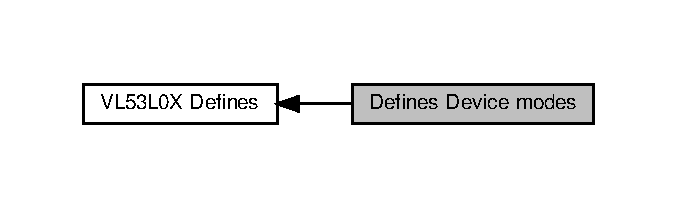
\includegraphics[width=325pt]{group__VL53L0X__define__DeviceModes__group}
\end{center}
\end{figure}
\subsection*{Macros}
\begin{DoxyCompactItemize}
\item 
\mbox{\Hypertarget{group__VL53L0X__define__DeviceModes__group_ga00e5de94c87b8ebe96347539e8da521b}\label{group__VL53L0X__define__DeviceModes__group_ga00e5de94c87b8ebe96347539e8da521b}} 
\#define {\bfseries V\+L53\+L0\+X\+\_\+\+D\+E\+V\+I\+C\+E\+M\+O\+D\+E\+\_\+\+S\+I\+N\+G\+L\+E\+\_\+\+R\+A\+N\+G\+I\+NG}~((V\+L53\+L0\+X\+\_\+\+Device\+Modes)  0)
\item 
\mbox{\Hypertarget{group__VL53L0X__define__DeviceModes__group_ga120c46888d1192a4f2dc146c4519b381}\label{group__VL53L0X__define__DeviceModes__group_ga120c46888d1192a4f2dc146c4519b381}} 
\#define {\bfseries V\+L53\+L0\+X\+\_\+\+D\+E\+V\+I\+C\+E\+M\+O\+D\+E\+\_\+\+C\+O\+N\+T\+I\+N\+U\+O\+U\+S\+\_\+\+R\+A\+N\+G\+I\+NG}~((V\+L53\+L0\+X\+\_\+\+Device\+Modes)  1)
\item 
\mbox{\Hypertarget{group__VL53L0X__define__DeviceModes__group_ga99363cd30b5ea4be01118d11f8fd5456}\label{group__VL53L0X__define__DeviceModes__group_ga99363cd30b5ea4be01118d11f8fd5456}} 
\#define {\bfseries V\+L53\+L0\+X\+\_\+\+D\+E\+V\+I\+C\+E\+M\+O\+D\+E\+\_\+\+S\+I\+N\+G\+L\+E\+\_\+\+H\+I\+S\+T\+O\+G\+R\+AM}~((V\+L53\+L0\+X\+\_\+\+Device\+Modes)  2)
\item 
\mbox{\Hypertarget{group__VL53L0X__define__DeviceModes__group_gae2b355c47714ed7fbac23de6d4c059dd}\label{group__VL53L0X__define__DeviceModes__group_gae2b355c47714ed7fbac23de6d4c059dd}} 
\#define {\bfseries V\+L53\+L0\+X\+\_\+\+D\+E\+V\+I\+C\+E\+M\+O\+D\+E\+\_\+\+C\+O\+N\+T\+I\+N\+U\+O\+U\+S\+\_\+\+T\+I\+M\+E\+D\+\_\+\+R\+A\+N\+G\+I\+NG}~((V\+L53\+L0\+X\+\_\+\+Device\+Modes) 3)
\item 
\mbox{\Hypertarget{group__VL53L0X__define__DeviceModes__group_ga3b112b695737e4a341a767e45a13c962}\label{group__VL53L0X__define__DeviceModes__group_ga3b112b695737e4a341a767e45a13c962}} 
\#define {\bfseries V\+L53\+L0\+X\+\_\+\+D\+E\+V\+I\+C\+E\+M\+O\+D\+E\+\_\+\+S\+I\+N\+G\+L\+E\+\_\+\+A\+LS}~((V\+L53\+L0\+X\+\_\+\+Device\+Modes) 10)
\item 
\mbox{\Hypertarget{group__VL53L0X__define__DeviceModes__group_ga1a4159e841975415b4938165533012bb}\label{group__VL53L0X__define__DeviceModes__group_ga1a4159e841975415b4938165533012bb}} 
\#define {\bfseries V\+L53\+L0\+X\+\_\+\+D\+E\+V\+I\+C\+E\+M\+O\+D\+E\+\_\+\+G\+P\+I\+O\+\_\+\+D\+R\+I\+VE}~((V\+L53\+L0\+X\+\_\+\+Device\+Modes) 20)
\item 
\mbox{\Hypertarget{group__VL53L0X__define__DeviceModes__group_ga65c383b38533235fcad65e5057ade145}\label{group__VL53L0X__define__DeviceModes__group_ga65c383b38533235fcad65e5057ade145}} 
\#define {\bfseries V\+L53\+L0\+X\+\_\+\+D\+E\+V\+I\+C\+E\+M\+O\+D\+E\+\_\+\+G\+P\+I\+O\+\_\+\+O\+SC}~((V\+L53\+L0\+X\+\_\+\+Device\+Modes) 21)
\end{DoxyCompactItemize}
\subsection*{Typedefs}
\begin{DoxyCompactItemize}
\item 
\mbox{\Hypertarget{group__VL53L0X__define__DeviceModes__group_ga93bfcd3ce1b784f332b9f3533320ab8f}\label{group__VL53L0X__define__DeviceModes__group_ga93bfcd3ce1b784f332b9f3533320ab8f}} 
typedef \hyperlink{vl53l0x__types_8h_aba7bc1797add20fe3efdf37ced1182c5}{uint8\+\_\+t} {\bfseries V\+L53\+L0\+X\+\_\+\+Device\+Modes}
\end{DoxyCompactItemize}


\subsection{Detailed Description}
Defines all possible modes for the device 
\hypertarget{group__VL53L0X__define__HistogramModes__group}{}\section{Defines Histogram modes}
\label{group__VL53L0X__define__HistogramModes__group}\index{Defines Histogram modes@{Defines Histogram modes}}
Collaboration diagram for Defines Histogram modes\+:\nopagebreak
\begin{figure}[H]
\begin{center}
\leavevmode
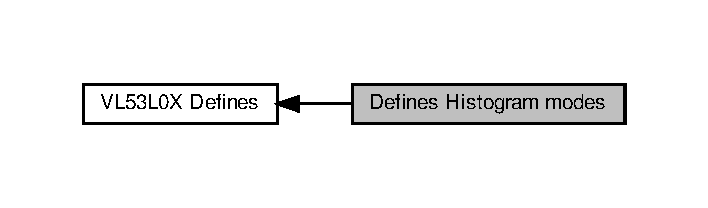
\includegraphics[width=340pt]{group__VL53L0X__define__HistogramModes__group}
\end{center}
\end{figure}
\subsection*{Macros}
\begin{DoxyCompactItemize}
\item 
\#define \hyperlink{group__VL53L0X__define__HistogramModes__group_ga1be8e446d952e6e70207159ede19e3f8}{V\+L53\+L0\+X\+\_\+\+H\+I\+S\+T\+O\+G\+R\+A\+M\+M\+O\+D\+E\+\_\+\+D\+I\+S\+A\+B\+L\+ED}~((V\+L53\+L0\+X\+\_\+\+Histogram\+Modes) 0)
\item 
\#define \hyperlink{group__VL53L0X__define__HistogramModes__group_ga1e0e3d9f63b1376c0e4e97cd23640674}{V\+L53\+L0\+X\+\_\+\+H\+I\+S\+T\+O\+G\+R\+A\+M\+M\+O\+D\+E\+\_\+\+R\+E\+F\+E\+R\+E\+N\+C\+E\+\_\+\+O\+N\+LY}~((V\+L53\+L0\+X\+\_\+\+Histogram\+Modes) 1)
\item 
\#define \hyperlink{group__VL53L0X__define__HistogramModes__group_gaf37229d15d3cb3330e4d8de4d49741dd}{V\+L53\+L0\+X\+\_\+\+H\+I\+S\+T\+O\+G\+R\+A\+M\+M\+O\+D\+E\+\_\+\+R\+E\+T\+U\+R\+N\+\_\+\+O\+N\+LY}~((V\+L53\+L0\+X\+\_\+\+Histogram\+Modes) 2)
\item 
\#define \hyperlink{group__VL53L0X__define__HistogramModes__group_gac06efee5e5499ec3a8c09d5a20a1d2b8}{V\+L53\+L0\+X\+\_\+\+H\+I\+S\+T\+O\+G\+R\+A\+M\+M\+O\+D\+E\+\_\+\+B\+O\+TH}~((V\+L53\+L0\+X\+\_\+\+Histogram\+Modes) 3)
\end{DoxyCompactItemize}
\subsection*{Typedefs}
\begin{DoxyCompactItemize}
\item 
\mbox{\Hypertarget{group__VL53L0X__define__HistogramModes__group_ga3248067155806886b6bf1b10eaa83ea4}\label{group__VL53L0X__define__HistogramModes__group_ga3248067155806886b6bf1b10eaa83ea4}} 
typedef \hyperlink{vl53l0x__types_8h_aba7bc1797add20fe3efdf37ced1182c5}{uint8\+\_\+t} {\bfseries V\+L53\+L0\+X\+\_\+\+Histogram\+Modes}
\end{DoxyCompactItemize}


\subsection{Detailed Description}
Defines all possible Histogram modes for the device 

\subsection{Macro Definition Documentation}
\mbox{\Hypertarget{group__VL53L0X__define__HistogramModes__group_gac06efee5e5499ec3a8c09d5a20a1d2b8}\label{group__VL53L0X__define__HistogramModes__group_gac06efee5e5499ec3a8c09d5a20a1d2b8}} 
\index{Defines Histogram modes@{Defines Histogram modes}!V\+L53\+L0\+X\+\_\+\+H\+I\+S\+T\+O\+G\+R\+A\+M\+M\+O\+D\+E\+\_\+\+B\+O\+TH@{V\+L53\+L0\+X\+\_\+\+H\+I\+S\+T\+O\+G\+R\+A\+M\+M\+O\+D\+E\+\_\+\+B\+O\+TH}}
\index{V\+L53\+L0\+X\+\_\+\+H\+I\+S\+T\+O\+G\+R\+A\+M\+M\+O\+D\+E\+\_\+\+B\+O\+TH@{V\+L53\+L0\+X\+\_\+\+H\+I\+S\+T\+O\+G\+R\+A\+M\+M\+O\+D\+E\+\_\+\+B\+O\+TH}!Defines Histogram modes@{Defines Histogram modes}}
\subsubsection{\texorpdfstring{V\+L53\+L0\+X\+\_\+\+H\+I\+S\+T\+O\+G\+R\+A\+M\+M\+O\+D\+E\+\_\+\+B\+O\+TH}{VL53L0X\_HISTOGRAMMODE\_BOTH}}
{\footnotesize\ttfamily \#define V\+L53\+L0\+X\+\_\+\+H\+I\+S\+T\+O\+G\+R\+A\+M\+M\+O\+D\+E\+\_\+\+B\+O\+TH~((V\+L53\+L0\+X\+\_\+\+Histogram\+Modes) 3)}

Histogram both Reference and Return Arrays \mbox{\Hypertarget{group__VL53L0X__define__HistogramModes__group_ga1be8e446d952e6e70207159ede19e3f8}\label{group__VL53L0X__define__HistogramModes__group_ga1be8e446d952e6e70207159ede19e3f8}} 
\index{Defines Histogram modes@{Defines Histogram modes}!V\+L53\+L0\+X\+\_\+\+H\+I\+S\+T\+O\+G\+R\+A\+M\+M\+O\+D\+E\+\_\+\+D\+I\+S\+A\+B\+L\+ED@{V\+L53\+L0\+X\+\_\+\+H\+I\+S\+T\+O\+G\+R\+A\+M\+M\+O\+D\+E\+\_\+\+D\+I\+S\+A\+B\+L\+ED}}
\index{V\+L53\+L0\+X\+\_\+\+H\+I\+S\+T\+O\+G\+R\+A\+M\+M\+O\+D\+E\+\_\+\+D\+I\+S\+A\+B\+L\+ED@{V\+L53\+L0\+X\+\_\+\+H\+I\+S\+T\+O\+G\+R\+A\+M\+M\+O\+D\+E\+\_\+\+D\+I\+S\+A\+B\+L\+ED}!Defines Histogram modes@{Defines Histogram modes}}
\subsubsection{\texorpdfstring{V\+L53\+L0\+X\+\_\+\+H\+I\+S\+T\+O\+G\+R\+A\+M\+M\+O\+D\+E\+\_\+\+D\+I\+S\+A\+B\+L\+ED}{VL53L0X\_HISTOGRAMMODE\_DISABLED}}
{\footnotesize\ttfamily \#define V\+L53\+L0\+X\+\_\+\+H\+I\+S\+T\+O\+G\+R\+A\+M\+M\+O\+D\+E\+\_\+\+D\+I\+S\+A\+B\+L\+ED~((V\+L53\+L0\+X\+\_\+\+Histogram\+Modes) 0)}

Histogram Disabled \mbox{\Hypertarget{group__VL53L0X__define__HistogramModes__group_ga1e0e3d9f63b1376c0e4e97cd23640674}\label{group__VL53L0X__define__HistogramModes__group_ga1e0e3d9f63b1376c0e4e97cd23640674}} 
\index{Defines Histogram modes@{Defines Histogram modes}!V\+L53\+L0\+X\+\_\+\+H\+I\+S\+T\+O\+G\+R\+A\+M\+M\+O\+D\+E\+\_\+\+R\+E\+F\+E\+R\+E\+N\+C\+E\+\_\+\+O\+N\+LY@{V\+L53\+L0\+X\+\_\+\+H\+I\+S\+T\+O\+G\+R\+A\+M\+M\+O\+D\+E\+\_\+\+R\+E\+F\+E\+R\+E\+N\+C\+E\+\_\+\+O\+N\+LY}}
\index{V\+L53\+L0\+X\+\_\+\+H\+I\+S\+T\+O\+G\+R\+A\+M\+M\+O\+D\+E\+\_\+\+R\+E\+F\+E\+R\+E\+N\+C\+E\+\_\+\+O\+N\+LY@{V\+L53\+L0\+X\+\_\+\+H\+I\+S\+T\+O\+G\+R\+A\+M\+M\+O\+D\+E\+\_\+\+R\+E\+F\+E\+R\+E\+N\+C\+E\+\_\+\+O\+N\+LY}!Defines Histogram modes@{Defines Histogram modes}}
\subsubsection{\texorpdfstring{V\+L53\+L0\+X\+\_\+\+H\+I\+S\+T\+O\+G\+R\+A\+M\+M\+O\+D\+E\+\_\+\+R\+E\+F\+E\+R\+E\+N\+C\+E\+\_\+\+O\+N\+LY}{VL53L0X\_HISTOGRAMMODE\_REFERENCE\_ONLY}}
{\footnotesize\ttfamily \#define V\+L53\+L0\+X\+\_\+\+H\+I\+S\+T\+O\+G\+R\+A\+M\+M\+O\+D\+E\+\_\+\+R\+E\+F\+E\+R\+E\+N\+C\+E\+\_\+\+O\+N\+LY~((V\+L53\+L0\+X\+\_\+\+Histogram\+Modes) 1)}

Histogram Reference array only \mbox{\Hypertarget{group__VL53L0X__define__HistogramModes__group_gaf37229d15d3cb3330e4d8de4d49741dd}\label{group__VL53L0X__define__HistogramModes__group_gaf37229d15d3cb3330e4d8de4d49741dd}} 
\index{Defines Histogram modes@{Defines Histogram modes}!V\+L53\+L0\+X\+\_\+\+H\+I\+S\+T\+O\+G\+R\+A\+M\+M\+O\+D\+E\+\_\+\+R\+E\+T\+U\+R\+N\+\_\+\+O\+N\+LY@{V\+L53\+L0\+X\+\_\+\+H\+I\+S\+T\+O\+G\+R\+A\+M\+M\+O\+D\+E\+\_\+\+R\+E\+T\+U\+R\+N\+\_\+\+O\+N\+LY}}
\index{V\+L53\+L0\+X\+\_\+\+H\+I\+S\+T\+O\+G\+R\+A\+M\+M\+O\+D\+E\+\_\+\+R\+E\+T\+U\+R\+N\+\_\+\+O\+N\+LY@{V\+L53\+L0\+X\+\_\+\+H\+I\+S\+T\+O\+G\+R\+A\+M\+M\+O\+D\+E\+\_\+\+R\+E\+T\+U\+R\+N\+\_\+\+O\+N\+LY}!Defines Histogram modes@{Defines Histogram modes}}
\subsubsection{\texorpdfstring{V\+L53\+L0\+X\+\_\+\+H\+I\+S\+T\+O\+G\+R\+A\+M\+M\+O\+D\+E\+\_\+\+R\+E\+T\+U\+R\+N\+\_\+\+O\+N\+LY}{VL53L0X\_HISTOGRAMMODE\_RETURN\_ONLY}}
{\footnotesize\ttfamily \#define V\+L53\+L0\+X\+\_\+\+H\+I\+S\+T\+O\+G\+R\+A\+M\+M\+O\+D\+E\+\_\+\+R\+E\+T\+U\+R\+N\+\_\+\+O\+N\+LY~((V\+L53\+L0\+X\+\_\+\+Histogram\+Modes) 2)}

Histogram Return array only 
\hypertarget{group__VL53L0X__define__PowerModes__group}{}\section{List of available Power Modes}
\label{group__VL53L0X__define__PowerModes__group}\index{List of available Power Modes@{List of available Power Modes}}
Collaboration diagram for List of available Power Modes\+:\nopagebreak
\begin{figure}[H]
\begin{center}
\leavevmode
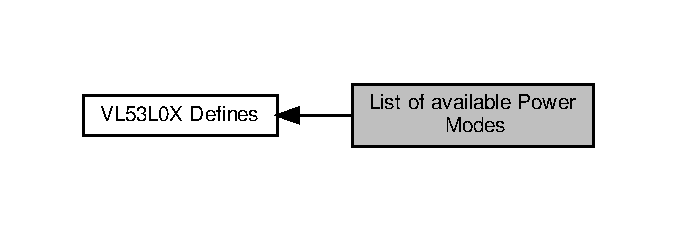
\includegraphics[width=325pt]{group__VL53L0X__define__PowerModes__group}
\end{center}
\end{figure}
\subsection*{Macros}
\begin{DoxyCompactItemize}
\item 
\#define \hyperlink{group__VL53L0X__define__PowerModes__group_gae816ea89b667d4dd40341ad1ad0cbeb7}{V\+L53\+L0\+X\+\_\+\+P\+O\+W\+E\+R\+M\+O\+D\+E\+\_\+\+S\+T\+A\+N\+D\+B\+Y\+\_\+\+L\+E\+V\+E\+L1}~((V\+L53\+L0\+X\+\_\+\+Power\+Modes) 0)
\item 
\#define \hyperlink{group__VL53L0X__define__PowerModes__group_gafd2e4343268551ef26445ca31332e01c}{V\+L53\+L0\+X\+\_\+\+P\+O\+W\+E\+R\+M\+O\+D\+E\+\_\+\+S\+T\+A\+N\+D\+B\+Y\+\_\+\+L\+E\+V\+E\+L2}~((V\+L53\+L0\+X\+\_\+\+Power\+Modes) 1)
\item 
\#define \hyperlink{group__VL53L0X__define__PowerModes__group_gadc8d4ccde38324e2b8731eb3d4964d74}{V\+L53\+L0\+X\+\_\+\+P\+O\+W\+E\+R\+M\+O\+D\+E\+\_\+\+I\+D\+L\+E\+\_\+\+L\+E\+V\+E\+L1}~((V\+L53\+L0\+X\+\_\+\+Power\+Modes) 2)
\item 
\#define \hyperlink{group__VL53L0X__define__PowerModes__group_gabd79d2665e85cec3cd18a2faaa103134}{V\+L53\+L0\+X\+\_\+\+P\+O\+W\+E\+R\+M\+O\+D\+E\+\_\+\+I\+D\+L\+E\+\_\+\+L\+E\+V\+E\+L2}~((V\+L53\+L0\+X\+\_\+\+Power\+Modes) 3)
\end{DoxyCompactItemize}
\subsection*{Typedefs}
\begin{DoxyCompactItemize}
\item 
\mbox{\Hypertarget{group__VL53L0X__define__PowerModes__group_ga1ddcb47e13a84eb97913d973ffeec2a2}\label{group__VL53L0X__define__PowerModes__group_ga1ddcb47e13a84eb97913d973ffeec2a2}} 
typedef \hyperlink{vl53l0x__types_8h_aba7bc1797add20fe3efdf37ced1182c5}{uint8\+\_\+t} {\bfseries V\+L53\+L0\+X\+\_\+\+Power\+Modes}
\end{DoxyCompactItemize}


\subsection{Detailed Description}
List of available Power Modes 

\subsection{Macro Definition Documentation}
\mbox{\Hypertarget{group__VL53L0X__define__PowerModes__group_gadc8d4ccde38324e2b8731eb3d4964d74}\label{group__VL53L0X__define__PowerModes__group_gadc8d4ccde38324e2b8731eb3d4964d74}} 
\index{List of available Power Modes@{List of available Power Modes}!V\+L53\+L0\+X\+\_\+\+P\+O\+W\+E\+R\+M\+O\+D\+E\+\_\+\+I\+D\+L\+E\+\_\+\+L\+E\+V\+E\+L1@{V\+L53\+L0\+X\+\_\+\+P\+O\+W\+E\+R\+M\+O\+D\+E\+\_\+\+I\+D\+L\+E\+\_\+\+L\+E\+V\+E\+L1}}
\index{V\+L53\+L0\+X\+\_\+\+P\+O\+W\+E\+R\+M\+O\+D\+E\+\_\+\+I\+D\+L\+E\+\_\+\+L\+E\+V\+E\+L1@{V\+L53\+L0\+X\+\_\+\+P\+O\+W\+E\+R\+M\+O\+D\+E\+\_\+\+I\+D\+L\+E\+\_\+\+L\+E\+V\+E\+L1}!List of available Power Modes@{List of available Power Modes}}
\subsubsection{\texorpdfstring{V\+L53\+L0\+X\+\_\+\+P\+O\+W\+E\+R\+M\+O\+D\+E\+\_\+\+I\+D\+L\+E\+\_\+\+L\+E\+V\+E\+L1}{VL53L0X\_POWERMODE\_IDLE\_LEVEL1}}
{\footnotesize\ttfamily \#define V\+L53\+L0\+X\+\_\+\+P\+O\+W\+E\+R\+M\+O\+D\+E\+\_\+\+I\+D\+L\+E\+\_\+\+L\+E\+V\+E\+L1~((V\+L53\+L0\+X\+\_\+\+Power\+Modes) 2)}

Idle level 1 \mbox{\Hypertarget{group__VL53L0X__define__PowerModes__group_gabd79d2665e85cec3cd18a2faaa103134}\label{group__VL53L0X__define__PowerModes__group_gabd79d2665e85cec3cd18a2faaa103134}} 
\index{List of available Power Modes@{List of available Power Modes}!V\+L53\+L0\+X\+\_\+\+P\+O\+W\+E\+R\+M\+O\+D\+E\+\_\+\+I\+D\+L\+E\+\_\+\+L\+E\+V\+E\+L2@{V\+L53\+L0\+X\+\_\+\+P\+O\+W\+E\+R\+M\+O\+D\+E\+\_\+\+I\+D\+L\+E\+\_\+\+L\+E\+V\+E\+L2}}
\index{V\+L53\+L0\+X\+\_\+\+P\+O\+W\+E\+R\+M\+O\+D\+E\+\_\+\+I\+D\+L\+E\+\_\+\+L\+E\+V\+E\+L2@{V\+L53\+L0\+X\+\_\+\+P\+O\+W\+E\+R\+M\+O\+D\+E\+\_\+\+I\+D\+L\+E\+\_\+\+L\+E\+V\+E\+L2}!List of available Power Modes@{List of available Power Modes}}
\subsubsection{\texorpdfstring{V\+L53\+L0\+X\+\_\+\+P\+O\+W\+E\+R\+M\+O\+D\+E\+\_\+\+I\+D\+L\+E\+\_\+\+L\+E\+V\+E\+L2}{VL53L0X\_POWERMODE\_IDLE\_LEVEL2}}
{\footnotesize\ttfamily \#define V\+L53\+L0\+X\+\_\+\+P\+O\+W\+E\+R\+M\+O\+D\+E\+\_\+\+I\+D\+L\+E\+\_\+\+L\+E\+V\+E\+L2~((V\+L53\+L0\+X\+\_\+\+Power\+Modes) 3)}

Idle level 2 \mbox{\Hypertarget{group__VL53L0X__define__PowerModes__group_gae816ea89b667d4dd40341ad1ad0cbeb7}\label{group__VL53L0X__define__PowerModes__group_gae816ea89b667d4dd40341ad1ad0cbeb7}} 
\index{List of available Power Modes@{List of available Power Modes}!V\+L53\+L0\+X\+\_\+\+P\+O\+W\+E\+R\+M\+O\+D\+E\+\_\+\+S\+T\+A\+N\+D\+B\+Y\+\_\+\+L\+E\+V\+E\+L1@{V\+L53\+L0\+X\+\_\+\+P\+O\+W\+E\+R\+M\+O\+D\+E\+\_\+\+S\+T\+A\+N\+D\+B\+Y\+\_\+\+L\+E\+V\+E\+L1}}
\index{V\+L53\+L0\+X\+\_\+\+P\+O\+W\+E\+R\+M\+O\+D\+E\+\_\+\+S\+T\+A\+N\+D\+B\+Y\+\_\+\+L\+E\+V\+E\+L1@{V\+L53\+L0\+X\+\_\+\+P\+O\+W\+E\+R\+M\+O\+D\+E\+\_\+\+S\+T\+A\+N\+D\+B\+Y\+\_\+\+L\+E\+V\+E\+L1}!List of available Power Modes@{List of available Power Modes}}
\subsubsection{\texorpdfstring{V\+L53\+L0\+X\+\_\+\+P\+O\+W\+E\+R\+M\+O\+D\+E\+\_\+\+S\+T\+A\+N\+D\+B\+Y\+\_\+\+L\+E\+V\+E\+L1}{VL53L0X\_POWERMODE\_STANDBY\_LEVEL1}}
{\footnotesize\ttfamily \#define V\+L53\+L0\+X\+\_\+\+P\+O\+W\+E\+R\+M\+O\+D\+E\+\_\+\+S\+T\+A\+N\+D\+B\+Y\+\_\+\+L\+E\+V\+E\+L1~((V\+L53\+L0\+X\+\_\+\+Power\+Modes) 0)}

Standby level 1 \mbox{\Hypertarget{group__VL53L0X__define__PowerModes__group_gafd2e4343268551ef26445ca31332e01c}\label{group__VL53L0X__define__PowerModes__group_gafd2e4343268551ef26445ca31332e01c}} 
\index{List of available Power Modes@{List of available Power Modes}!V\+L53\+L0\+X\+\_\+\+P\+O\+W\+E\+R\+M\+O\+D\+E\+\_\+\+S\+T\+A\+N\+D\+B\+Y\+\_\+\+L\+E\+V\+E\+L2@{V\+L53\+L0\+X\+\_\+\+P\+O\+W\+E\+R\+M\+O\+D\+E\+\_\+\+S\+T\+A\+N\+D\+B\+Y\+\_\+\+L\+E\+V\+E\+L2}}
\index{V\+L53\+L0\+X\+\_\+\+P\+O\+W\+E\+R\+M\+O\+D\+E\+\_\+\+S\+T\+A\+N\+D\+B\+Y\+\_\+\+L\+E\+V\+E\+L2@{V\+L53\+L0\+X\+\_\+\+P\+O\+W\+E\+R\+M\+O\+D\+E\+\_\+\+S\+T\+A\+N\+D\+B\+Y\+\_\+\+L\+E\+V\+E\+L2}!List of available Power Modes@{List of available Power Modes}}
\subsubsection{\texorpdfstring{V\+L53\+L0\+X\+\_\+\+P\+O\+W\+E\+R\+M\+O\+D\+E\+\_\+\+S\+T\+A\+N\+D\+B\+Y\+\_\+\+L\+E\+V\+E\+L2}{VL53L0X\_POWERMODE\_STANDBY\_LEVEL2}}
{\footnotesize\ttfamily \#define V\+L53\+L0\+X\+\_\+\+P\+O\+W\+E\+R\+M\+O\+D\+E\+\_\+\+S\+T\+A\+N\+D\+B\+Y\+\_\+\+L\+E\+V\+E\+L2~((V\+L53\+L0\+X\+\_\+\+Power\+Modes) 1)}

Standby level 2 
\hypertarget{group__VL53L0X__define__State__group}{}\section{Defines the current status of the device}
\label{group__VL53L0X__define__State__group}\index{Defines the current status of the device@{Defines the current status of the device}}
Collaboration diagram for Defines the current status of the device\+:\nopagebreak
\begin{figure}[H]
\begin{center}
\leavevmode
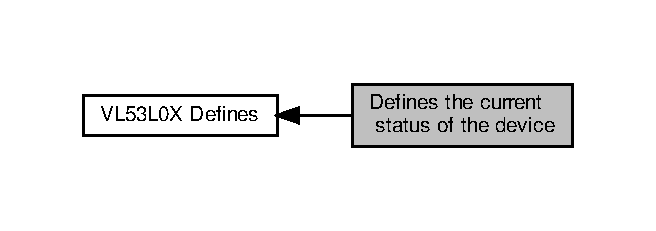
\includegraphics[width=315pt]{group__VL53L0X__define__State__group}
\end{center}
\end{figure}
\subsection*{Macros}
\begin{DoxyCompactItemize}
\item 
\#define \hyperlink{group__VL53L0X__define__State__group_gadc7ed3137681a4fcf1021e9e55a9dc35}{V\+L53\+L0\+X\+\_\+\+S\+T\+A\+T\+E\+\_\+\+P\+O\+W\+E\+R\+D\+O\+WN}~((V\+L53\+L0\+X\+\_\+\+State)  0)
\item 
\#define \hyperlink{group__VL53L0X__define__State__group_gae1ac367449ae3fdd4f508c642fe1c530}{V\+L53\+L0\+X\+\_\+\+S\+T\+A\+T\+E\+\_\+\+W\+A\+I\+T\+\_\+\+S\+T\+A\+T\+I\+C\+I\+N\+IT}~((V\+L53\+L0\+X\+\_\+\+State)  1)
\item 
\#define \hyperlink{group__VL53L0X__define__State__group_gaf46fb23dab2f5344860a10c1938885b2}{V\+L53\+L0\+X\+\_\+\+S\+T\+A\+T\+E\+\_\+\+S\+T\+A\+N\+D\+BY}~((V\+L53\+L0\+X\+\_\+\+State)  2)
\item 
\#define \hyperlink{group__VL53L0X__define__State__group_ga074c4b38507044ec430d5a0254f5b57d}{V\+L53\+L0\+X\+\_\+\+S\+T\+A\+T\+E\+\_\+\+I\+D\+LE}~((V\+L53\+L0\+X\+\_\+\+State)  3)
\item 
\#define \hyperlink{group__VL53L0X__define__State__group_gae6638c8138a8dcfe752e9ebd6e2bcf40}{V\+L53\+L0\+X\+\_\+\+S\+T\+A\+T\+E\+\_\+\+R\+U\+N\+N\+I\+NG}~((V\+L53\+L0\+X\+\_\+\+State)  4)
\item 
\#define \hyperlink{group__VL53L0X__define__State__group_ga3ebef117a1cd195911d8d988c2778704}{V\+L53\+L0\+X\+\_\+\+S\+T\+A\+T\+E\+\_\+\+U\+N\+K\+N\+O\+WN}~((V\+L53\+L0\+X\+\_\+\+State)  98)
\item 
\#define \hyperlink{group__VL53L0X__define__State__group_ga29a332f5cb56dfc3a521e6f5955ea29b}{V\+L53\+L0\+X\+\_\+\+S\+T\+A\+T\+E\+\_\+\+E\+R\+R\+OR}~((V\+L53\+L0\+X\+\_\+\+State)  99)
\end{DoxyCompactItemize}
\subsection*{Typedefs}
\begin{DoxyCompactItemize}
\item 
\mbox{\Hypertarget{group__VL53L0X__define__State__group_gad67e4c805db1a6d472ac78b814f7ef70}\label{group__VL53L0X__define__State__group_gad67e4c805db1a6d472ac78b814f7ef70}} 
typedef \hyperlink{vl53l0x__types_8h_aba7bc1797add20fe3efdf37ced1182c5}{uint8\+\_\+t} {\bfseries V\+L53\+L0\+X\+\_\+\+State}
\end{DoxyCompactItemize}


\subsection{Detailed Description}
Defines the current status of the device 

\subsection{Macro Definition Documentation}
\mbox{\Hypertarget{group__VL53L0X__define__State__group_ga29a332f5cb56dfc3a521e6f5955ea29b}\label{group__VL53L0X__define__State__group_ga29a332f5cb56dfc3a521e6f5955ea29b}} 
\index{Defines the current status of the device@{Defines the current status of the device}!V\+L53\+L0\+X\+\_\+\+S\+T\+A\+T\+E\+\_\+\+E\+R\+R\+OR@{V\+L53\+L0\+X\+\_\+\+S\+T\+A\+T\+E\+\_\+\+E\+R\+R\+OR}}
\index{V\+L53\+L0\+X\+\_\+\+S\+T\+A\+T\+E\+\_\+\+E\+R\+R\+OR@{V\+L53\+L0\+X\+\_\+\+S\+T\+A\+T\+E\+\_\+\+E\+R\+R\+OR}!Defines the current status of the device@{Defines the current status of the device}}
\subsubsection{\texorpdfstring{V\+L53\+L0\+X\+\_\+\+S\+T\+A\+T\+E\+\_\+\+E\+R\+R\+OR}{VL53L0X\_STATE\_ERROR}}
{\footnotesize\ttfamily \#define V\+L53\+L0\+X\+\_\+\+S\+T\+A\+T\+E\+\_\+\+E\+R\+R\+OR~((V\+L53\+L0\+X\+\_\+\+State)  99)}

Device is in error state and need to be rebooted \mbox{\Hypertarget{group__VL53L0X__define__State__group_ga074c4b38507044ec430d5a0254f5b57d}\label{group__VL53L0X__define__State__group_ga074c4b38507044ec430d5a0254f5b57d}} 
\index{Defines the current status of the device@{Defines the current status of the device}!V\+L53\+L0\+X\+\_\+\+S\+T\+A\+T\+E\+\_\+\+I\+D\+LE@{V\+L53\+L0\+X\+\_\+\+S\+T\+A\+T\+E\+\_\+\+I\+D\+LE}}
\index{V\+L53\+L0\+X\+\_\+\+S\+T\+A\+T\+E\+\_\+\+I\+D\+LE@{V\+L53\+L0\+X\+\_\+\+S\+T\+A\+T\+E\+\_\+\+I\+D\+LE}!Defines the current status of the device@{Defines the current status of the device}}
\subsubsection{\texorpdfstring{V\+L53\+L0\+X\+\_\+\+S\+T\+A\+T\+E\+\_\+\+I\+D\+LE}{VL53L0X\_STATE\_IDLE}}
{\footnotesize\ttfamily \#define V\+L53\+L0\+X\+\_\+\+S\+T\+A\+T\+E\+\_\+\+I\+D\+LE~((V\+L53\+L0\+X\+\_\+\+State)  3)}

Device has been initialized and ready to do measurements \mbox{\Hypertarget{group__VL53L0X__define__State__group_gadc7ed3137681a4fcf1021e9e55a9dc35}\label{group__VL53L0X__define__State__group_gadc7ed3137681a4fcf1021e9e55a9dc35}} 
\index{Defines the current status of the device@{Defines the current status of the device}!V\+L53\+L0\+X\+\_\+\+S\+T\+A\+T\+E\+\_\+\+P\+O\+W\+E\+R\+D\+O\+WN@{V\+L53\+L0\+X\+\_\+\+S\+T\+A\+T\+E\+\_\+\+P\+O\+W\+E\+R\+D\+O\+WN}}
\index{V\+L53\+L0\+X\+\_\+\+S\+T\+A\+T\+E\+\_\+\+P\+O\+W\+E\+R\+D\+O\+WN@{V\+L53\+L0\+X\+\_\+\+S\+T\+A\+T\+E\+\_\+\+P\+O\+W\+E\+R\+D\+O\+WN}!Defines the current status of the device@{Defines the current status of the device}}
\subsubsection{\texorpdfstring{V\+L53\+L0\+X\+\_\+\+S\+T\+A\+T\+E\+\_\+\+P\+O\+W\+E\+R\+D\+O\+WN}{VL53L0X\_STATE\_POWERDOWN}}
{\footnotesize\ttfamily \#define V\+L53\+L0\+X\+\_\+\+S\+T\+A\+T\+E\+\_\+\+P\+O\+W\+E\+R\+D\+O\+WN~((V\+L53\+L0\+X\+\_\+\+State)  0)}

Device is in HW reset \mbox{\Hypertarget{group__VL53L0X__define__State__group_gae6638c8138a8dcfe752e9ebd6e2bcf40}\label{group__VL53L0X__define__State__group_gae6638c8138a8dcfe752e9ebd6e2bcf40}} 
\index{Defines the current status of the device@{Defines the current status of the device}!V\+L53\+L0\+X\+\_\+\+S\+T\+A\+T\+E\+\_\+\+R\+U\+N\+N\+I\+NG@{V\+L53\+L0\+X\+\_\+\+S\+T\+A\+T\+E\+\_\+\+R\+U\+N\+N\+I\+NG}}
\index{V\+L53\+L0\+X\+\_\+\+S\+T\+A\+T\+E\+\_\+\+R\+U\+N\+N\+I\+NG@{V\+L53\+L0\+X\+\_\+\+S\+T\+A\+T\+E\+\_\+\+R\+U\+N\+N\+I\+NG}!Defines the current status of the device@{Defines the current status of the device}}
\subsubsection{\texorpdfstring{V\+L53\+L0\+X\+\_\+\+S\+T\+A\+T\+E\+\_\+\+R\+U\+N\+N\+I\+NG}{VL53L0X\_STATE\_RUNNING}}
{\footnotesize\ttfamily \#define V\+L53\+L0\+X\+\_\+\+S\+T\+A\+T\+E\+\_\+\+R\+U\+N\+N\+I\+NG~((V\+L53\+L0\+X\+\_\+\+State)  4)}

Device is performing measurement \mbox{\Hypertarget{group__VL53L0X__define__State__group_gaf46fb23dab2f5344860a10c1938885b2}\label{group__VL53L0X__define__State__group_gaf46fb23dab2f5344860a10c1938885b2}} 
\index{Defines the current status of the device@{Defines the current status of the device}!V\+L53\+L0\+X\+\_\+\+S\+T\+A\+T\+E\+\_\+\+S\+T\+A\+N\+D\+BY@{V\+L53\+L0\+X\+\_\+\+S\+T\+A\+T\+E\+\_\+\+S\+T\+A\+N\+D\+BY}}
\index{V\+L53\+L0\+X\+\_\+\+S\+T\+A\+T\+E\+\_\+\+S\+T\+A\+N\+D\+BY@{V\+L53\+L0\+X\+\_\+\+S\+T\+A\+T\+E\+\_\+\+S\+T\+A\+N\+D\+BY}!Defines the current status of the device@{Defines the current status of the device}}
\subsubsection{\texorpdfstring{V\+L53\+L0\+X\+\_\+\+S\+T\+A\+T\+E\+\_\+\+S\+T\+A\+N\+D\+BY}{VL53L0X\_STATE\_STANDBY}}
{\footnotesize\ttfamily \#define V\+L53\+L0\+X\+\_\+\+S\+T\+A\+T\+E\+\_\+\+S\+T\+A\+N\+D\+BY~((V\+L53\+L0\+X\+\_\+\+State)  2)}

Device is in Low power Standby mode \mbox{\Hypertarget{group__VL53L0X__define__State__group_ga3ebef117a1cd195911d8d988c2778704}\label{group__VL53L0X__define__State__group_ga3ebef117a1cd195911d8d988c2778704}} 
\index{Defines the current status of the device@{Defines the current status of the device}!V\+L53\+L0\+X\+\_\+\+S\+T\+A\+T\+E\+\_\+\+U\+N\+K\+N\+O\+WN@{V\+L53\+L0\+X\+\_\+\+S\+T\+A\+T\+E\+\_\+\+U\+N\+K\+N\+O\+WN}}
\index{V\+L53\+L0\+X\+\_\+\+S\+T\+A\+T\+E\+\_\+\+U\+N\+K\+N\+O\+WN@{V\+L53\+L0\+X\+\_\+\+S\+T\+A\+T\+E\+\_\+\+U\+N\+K\+N\+O\+WN}!Defines the current status of the device@{Defines the current status of the device}}
\subsubsection{\texorpdfstring{V\+L53\+L0\+X\+\_\+\+S\+T\+A\+T\+E\+\_\+\+U\+N\+K\+N\+O\+WN}{VL53L0X\_STATE\_UNKNOWN}}
{\footnotesize\ttfamily \#define V\+L53\+L0\+X\+\_\+\+S\+T\+A\+T\+E\+\_\+\+U\+N\+K\+N\+O\+WN~((V\+L53\+L0\+X\+\_\+\+State)  98)}

Device is in unknown state and need to be rebooted \mbox{\Hypertarget{group__VL53L0X__define__State__group_gae1ac367449ae3fdd4f508c642fe1c530}\label{group__VL53L0X__define__State__group_gae1ac367449ae3fdd4f508c642fe1c530}} 
\index{Defines the current status of the device@{Defines the current status of the device}!V\+L53\+L0\+X\+\_\+\+S\+T\+A\+T\+E\+\_\+\+W\+A\+I\+T\+\_\+\+S\+T\+A\+T\+I\+C\+I\+N\+IT@{V\+L53\+L0\+X\+\_\+\+S\+T\+A\+T\+E\+\_\+\+W\+A\+I\+T\+\_\+\+S\+T\+A\+T\+I\+C\+I\+N\+IT}}
\index{V\+L53\+L0\+X\+\_\+\+S\+T\+A\+T\+E\+\_\+\+W\+A\+I\+T\+\_\+\+S\+T\+A\+T\+I\+C\+I\+N\+IT@{V\+L53\+L0\+X\+\_\+\+S\+T\+A\+T\+E\+\_\+\+W\+A\+I\+T\+\_\+\+S\+T\+A\+T\+I\+C\+I\+N\+IT}!Defines the current status of the device@{Defines the current status of the device}}
\subsubsection{\texorpdfstring{V\+L53\+L0\+X\+\_\+\+S\+T\+A\+T\+E\+\_\+\+W\+A\+I\+T\+\_\+\+S\+T\+A\+T\+I\+C\+I\+N\+IT}{VL53L0X\_STATE\_WAIT\_STATICINIT}}
{\footnotesize\ttfamily \#define V\+L53\+L0\+X\+\_\+\+S\+T\+A\+T\+E\+\_\+\+W\+A\+I\+T\+\_\+\+S\+T\+A\+T\+I\+C\+I\+N\+IT~((V\+L53\+L0\+X\+\_\+\+State)  1)}

Device is initialized and wait for static initialization 
\hypertarget{group__VL53L0X__define__InterruptPolarity__group}{}\section{Defines the Polarity}
\label{group__VL53L0X__define__InterruptPolarity__group}\index{Defines the Polarity@{Defines the Polarity}}
Collaboration diagram for Defines the Polarity\+:\nopagebreak
\begin{figure}[H]
\begin{center}
\leavevmode
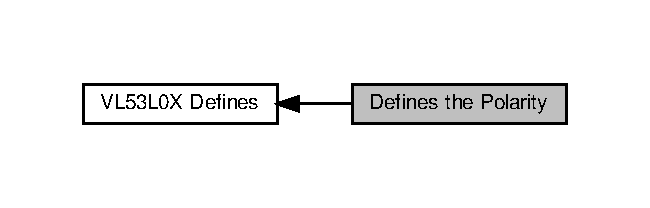
\includegraphics[width=312pt]{group__VL53L0X__define__InterruptPolarity__group}
\end{center}
\end{figure}
\subsection*{Macros}
\begin{DoxyCompactItemize}
\item 
\#define \hyperlink{group__VL53L0X__define__InterruptPolarity__group_ga67bf93a2c17680cc6ffcdd6834de1359}{V\+L53\+L0\+X\+\_\+\+I\+N\+T\+E\+R\+R\+U\+P\+T\+P\+O\+L\+A\+R\+I\+T\+Y\+\_\+\+L\+OW}~((V\+L53\+L0\+X\+\_\+\+Interrupt\+Polarity)    0)
\item 
\#define \hyperlink{group__VL53L0X__define__InterruptPolarity__group_gae0e72bee296015e468adcbb70db057d4}{V\+L53\+L0\+X\+\_\+\+I\+N\+T\+E\+R\+R\+U\+P\+T\+P\+O\+L\+A\+R\+I\+T\+Y\+\_\+\+H\+I\+GH}~((V\+L53\+L0\+X\+\_\+\+Interrupt\+Polarity)    1)
\end{DoxyCompactItemize}
\subsection*{Typedefs}
\begin{DoxyCompactItemize}
\item 
\mbox{\Hypertarget{group__VL53L0X__define__InterruptPolarity__group_ga2e3d6ac26e194574e08b27eee33922b5}\label{group__VL53L0X__define__InterruptPolarity__group_ga2e3d6ac26e194574e08b27eee33922b5}} 
typedef \hyperlink{vl53l0x__types_8h_aba7bc1797add20fe3efdf37ced1182c5}{uint8\+\_\+t} {\bfseries V\+L53\+L0\+X\+\_\+\+Interrupt\+Polarity}
\end{DoxyCompactItemize}


\subsection{Detailed Description}
of the Interrupt Defines the Polarity of the Interrupt 

\subsection{Macro Definition Documentation}
\mbox{\Hypertarget{group__VL53L0X__define__InterruptPolarity__group_gae0e72bee296015e468adcbb70db057d4}\label{group__VL53L0X__define__InterruptPolarity__group_gae0e72bee296015e468adcbb70db057d4}} 
\index{Defines the Polarity@{Defines the Polarity}!V\+L53\+L0\+X\+\_\+\+I\+N\+T\+E\+R\+R\+U\+P\+T\+P\+O\+L\+A\+R\+I\+T\+Y\+\_\+\+H\+I\+GH@{V\+L53\+L0\+X\+\_\+\+I\+N\+T\+E\+R\+R\+U\+P\+T\+P\+O\+L\+A\+R\+I\+T\+Y\+\_\+\+H\+I\+GH}}
\index{V\+L53\+L0\+X\+\_\+\+I\+N\+T\+E\+R\+R\+U\+P\+T\+P\+O\+L\+A\+R\+I\+T\+Y\+\_\+\+H\+I\+GH@{V\+L53\+L0\+X\+\_\+\+I\+N\+T\+E\+R\+R\+U\+P\+T\+P\+O\+L\+A\+R\+I\+T\+Y\+\_\+\+H\+I\+GH}!Defines the Polarity@{Defines the Polarity}}
\subsubsection{\texorpdfstring{V\+L53\+L0\+X\+\_\+\+I\+N\+T\+E\+R\+R\+U\+P\+T\+P\+O\+L\+A\+R\+I\+T\+Y\+\_\+\+H\+I\+GH}{VL53L0X\_INTERRUPTPOLARITY\_HIGH}}
{\footnotesize\ttfamily \#define V\+L53\+L0\+X\+\_\+\+I\+N\+T\+E\+R\+R\+U\+P\+T\+P\+O\+L\+A\+R\+I\+T\+Y\+\_\+\+H\+I\+GH~((V\+L53\+L0\+X\+\_\+\+Interrupt\+Polarity)    1)}

Set active high polarity best setup for rising edge. \mbox{\Hypertarget{group__VL53L0X__define__InterruptPolarity__group_ga67bf93a2c17680cc6ffcdd6834de1359}\label{group__VL53L0X__define__InterruptPolarity__group_ga67bf93a2c17680cc6ffcdd6834de1359}} 
\index{Defines the Polarity@{Defines the Polarity}!V\+L53\+L0\+X\+\_\+\+I\+N\+T\+E\+R\+R\+U\+P\+T\+P\+O\+L\+A\+R\+I\+T\+Y\+\_\+\+L\+OW@{V\+L53\+L0\+X\+\_\+\+I\+N\+T\+E\+R\+R\+U\+P\+T\+P\+O\+L\+A\+R\+I\+T\+Y\+\_\+\+L\+OW}}
\index{V\+L53\+L0\+X\+\_\+\+I\+N\+T\+E\+R\+R\+U\+P\+T\+P\+O\+L\+A\+R\+I\+T\+Y\+\_\+\+L\+OW@{V\+L53\+L0\+X\+\_\+\+I\+N\+T\+E\+R\+R\+U\+P\+T\+P\+O\+L\+A\+R\+I\+T\+Y\+\_\+\+L\+OW}!Defines the Polarity@{Defines the Polarity}}
\subsubsection{\texorpdfstring{V\+L53\+L0\+X\+\_\+\+I\+N\+T\+E\+R\+R\+U\+P\+T\+P\+O\+L\+A\+R\+I\+T\+Y\+\_\+\+L\+OW}{VL53L0X\_INTERRUPTPOLARITY\_LOW}}
{\footnotesize\ttfamily \#define V\+L53\+L0\+X\+\_\+\+I\+N\+T\+E\+R\+R\+U\+P\+T\+P\+O\+L\+A\+R\+I\+T\+Y\+\_\+\+L\+OW~((V\+L53\+L0\+X\+\_\+\+Interrupt\+Polarity)    0)}

Set active low polarity best setup for falling edge. 
\hypertarget{group__VL53L0X__define__VcselPeriod__group}{}\section{Vcsel Period Defines}
\label{group__VL53L0X__define__VcselPeriod__group}\index{Vcsel Period Defines@{Vcsel Period Defines}}
Collaboration diagram for Vcsel Period Defines\+:\nopagebreak
\begin{figure}[H]
\begin{center}
\leavevmode
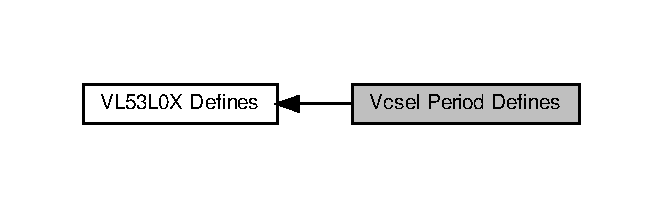
\includegraphics[width=318pt]{group__VL53L0X__define__VcselPeriod__group}
\end{center}
\end{figure}
\subsection*{Macros}
\begin{DoxyCompactItemize}
\item 
\#define \hyperlink{group__VL53L0X__define__VcselPeriod__group_ga9f8509e5364d1686c7add7e8642671a1}{V\+L53\+L0\+X\+\_\+\+V\+C\+S\+E\+L\+\_\+\+P\+E\+R\+I\+O\+D\+\_\+\+P\+R\+E\+\_\+\+R\+A\+N\+GE}~((V\+L53\+L0\+X\+\_\+\+Vcsel\+Period) 0)
\item 
\#define \hyperlink{group__VL53L0X__define__VcselPeriod__group_gaef30f6308508fde849425643076b63a3}{V\+L53\+L0\+X\+\_\+\+V\+C\+S\+E\+L\+\_\+\+P\+E\+R\+I\+O\+D\+\_\+\+F\+I\+N\+A\+L\+\_\+\+R\+A\+N\+GE}~((V\+L53\+L0\+X\+\_\+\+Vcsel\+Period) 1)
\end{DoxyCompactItemize}
\subsection*{Typedefs}
\begin{DoxyCompactItemize}
\item 
\mbox{\Hypertarget{group__VL53L0X__define__VcselPeriod__group_gaacc48b699574bf03e9b71a7a2dbcf64a}\label{group__VL53L0X__define__VcselPeriod__group_gaacc48b699574bf03e9b71a7a2dbcf64a}} 
typedef \hyperlink{vl53l0x__types_8h_aba7bc1797add20fe3efdf37ced1182c5}{uint8\+\_\+t} {\bfseries V\+L53\+L0\+X\+\_\+\+Vcsel\+Period}
\end{DoxyCompactItemize}


\subsection{Detailed Description}
Defines the range measurement for which to access the vcsel period. 

\subsection{Macro Definition Documentation}
\mbox{\Hypertarget{group__VL53L0X__define__VcselPeriod__group_gaef30f6308508fde849425643076b63a3}\label{group__VL53L0X__define__VcselPeriod__group_gaef30f6308508fde849425643076b63a3}} 
\index{Vcsel Period Defines@{Vcsel Period Defines}!V\+L53\+L0\+X\+\_\+\+V\+C\+S\+E\+L\+\_\+\+P\+E\+R\+I\+O\+D\+\_\+\+F\+I\+N\+A\+L\+\_\+\+R\+A\+N\+GE@{V\+L53\+L0\+X\+\_\+\+V\+C\+S\+E\+L\+\_\+\+P\+E\+R\+I\+O\+D\+\_\+\+F\+I\+N\+A\+L\+\_\+\+R\+A\+N\+GE}}
\index{V\+L53\+L0\+X\+\_\+\+V\+C\+S\+E\+L\+\_\+\+P\+E\+R\+I\+O\+D\+\_\+\+F\+I\+N\+A\+L\+\_\+\+R\+A\+N\+GE@{V\+L53\+L0\+X\+\_\+\+V\+C\+S\+E\+L\+\_\+\+P\+E\+R\+I\+O\+D\+\_\+\+F\+I\+N\+A\+L\+\_\+\+R\+A\+N\+GE}!Vcsel Period Defines@{Vcsel Period Defines}}
\subsubsection{\texorpdfstring{V\+L53\+L0\+X\+\_\+\+V\+C\+S\+E\+L\+\_\+\+P\+E\+R\+I\+O\+D\+\_\+\+F\+I\+N\+A\+L\+\_\+\+R\+A\+N\+GE}{VL53L0X\_VCSEL\_PERIOD\_FINAL\_RANGE}}
{\footnotesize\ttfamily \#define V\+L53\+L0\+X\+\_\+\+V\+C\+S\+E\+L\+\_\+\+P\+E\+R\+I\+O\+D\+\_\+\+F\+I\+N\+A\+L\+\_\+\+R\+A\+N\+GE~((V\+L53\+L0\+X\+\_\+\+Vcsel\+Period) 1)}

Identifies the final range vcsel period. \mbox{\Hypertarget{group__VL53L0X__define__VcselPeriod__group_ga9f8509e5364d1686c7add7e8642671a1}\label{group__VL53L0X__define__VcselPeriod__group_ga9f8509e5364d1686c7add7e8642671a1}} 
\index{Vcsel Period Defines@{Vcsel Period Defines}!V\+L53\+L0\+X\+\_\+\+V\+C\+S\+E\+L\+\_\+\+P\+E\+R\+I\+O\+D\+\_\+\+P\+R\+E\+\_\+\+R\+A\+N\+GE@{V\+L53\+L0\+X\+\_\+\+V\+C\+S\+E\+L\+\_\+\+P\+E\+R\+I\+O\+D\+\_\+\+P\+R\+E\+\_\+\+R\+A\+N\+GE}}
\index{V\+L53\+L0\+X\+\_\+\+V\+C\+S\+E\+L\+\_\+\+P\+E\+R\+I\+O\+D\+\_\+\+P\+R\+E\+\_\+\+R\+A\+N\+GE@{V\+L53\+L0\+X\+\_\+\+V\+C\+S\+E\+L\+\_\+\+P\+E\+R\+I\+O\+D\+\_\+\+P\+R\+E\+\_\+\+R\+A\+N\+GE}!Vcsel Period Defines@{Vcsel Period Defines}}
\subsubsection{\texorpdfstring{V\+L53\+L0\+X\+\_\+\+V\+C\+S\+E\+L\+\_\+\+P\+E\+R\+I\+O\+D\+\_\+\+P\+R\+E\+\_\+\+R\+A\+N\+GE}{VL53L0X\_VCSEL\_PERIOD\_PRE\_RANGE}}
{\footnotesize\ttfamily \#define V\+L53\+L0\+X\+\_\+\+V\+C\+S\+E\+L\+\_\+\+P\+E\+R\+I\+O\+D\+\_\+\+P\+R\+E\+\_\+\+R\+A\+N\+GE~((V\+L53\+L0\+X\+\_\+\+Vcsel\+Period) 0)}

Identifies the pre-\/range vcsel period. 
\hypertarget{group__VL53L0X__define__SchedulerSequence__group}{}\section{Defines the steps}
\label{group__VL53L0X__define__SchedulerSequence__group}\index{Defines the steps@{Defines the steps}}
Collaboration diagram for Defines the steps\+:\nopagebreak
\begin{figure}[H]
\begin{center}
\leavevmode
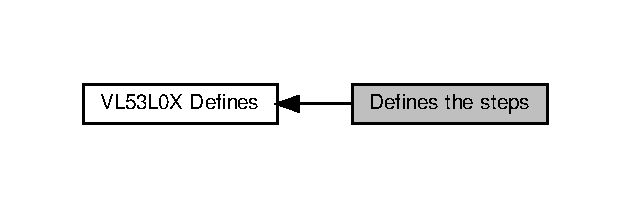
\includegraphics[width=303pt]{group__VL53L0X__define__SchedulerSequence__group}
\end{center}
\end{figure}
\subsection*{Classes}
\begin{DoxyCompactItemize}
\item 
struct \hyperlink{structVL53L0X__SchedulerSequenceSteps__t}{V\+L53\+L0\+X\+\_\+\+Scheduler\+Sequence\+Steps\+\_\+t}
\end{DoxyCompactItemize}


\subsection{Detailed Description}
carried out by the scheduler during a range measurement.

Defines the states of all the steps in the scheduler i.\+e. enabled/disabled. 
\hypertarget{group__VL53L0X__define__SequenceStepId__group}{}\section{Defines the Polarity}
\label{group__VL53L0X__define__SequenceStepId__group}\index{Defines the Polarity@{Defines the Polarity}}
Collaboration diagram for Defines the Polarity\+:\nopagebreak
\begin{figure}[H]
\begin{center}
\leavevmode
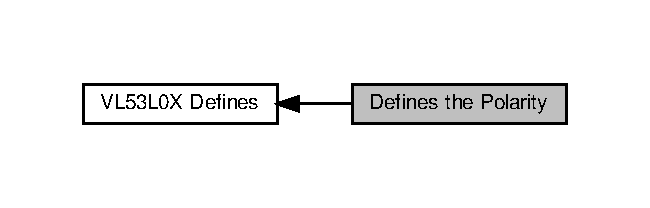
\includegraphics[width=312pt]{group__VL53L0X__define__SequenceStepId__group}
\end{center}
\end{figure}
\subsection*{Macros}
\begin{DoxyCompactItemize}
\item 
\#define \hyperlink{group__VL53L0X__define__SequenceStepId__group_gaf4a4c4ee04b303f4f08f2d1f4fae9811}{V\+L53\+L0\+X\+\_\+\+S\+E\+Q\+U\+E\+N\+C\+E\+S\+T\+E\+P\+\_\+\+T\+CC}~((V\+L53\+L0\+X\+\_\+\+Vcsel\+Period) 0)
\item 
\#define \hyperlink{group__VL53L0X__define__SequenceStepId__group_ga86ce83e9efbd7afbf1f95f1f2988e35b}{V\+L53\+L0\+X\+\_\+\+S\+E\+Q\+U\+E\+N\+C\+E\+S\+T\+E\+P\+\_\+\+D\+SS}~((V\+L53\+L0\+X\+\_\+\+Vcsel\+Period) 1)
\item 
\#define \hyperlink{group__VL53L0X__define__SequenceStepId__group_gab8dded683178089ec7a0cc4db1bf8655}{V\+L53\+L0\+X\+\_\+\+S\+E\+Q\+U\+E\+N\+C\+E\+S\+T\+E\+P\+\_\+\+M\+S\+RC}~((V\+L53\+L0\+X\+\_\+\+Vcsel\+Period) 2)
\item 
\#define \hyperlink{group__VL53L0X__define__SequenceStepId__group_gacb25b6b997a4baed47fbd5a5d6cc8214}{V\+L53\+L0\+X\+\_\+\+S\+E\+Q\+U\+E\+N\+C\+E\+S\+T\+E\+P\+\_\+\+P\+R\+E\+\_\+\+R\+A\+N\+GE}~((V\+L53\+L0\+X\+\_\+\+Vcsel\+Period) 3)
\item 
\#define \hyperlink{group__VL53L0X__define__SequenceStepId__group_ga54b2e024f4299dbd2b53128b82c5fcd0}{V\+L53\+L0\+X\+\_\+\+S\+E\+Q\+U\+E\+N\+C\+E\+S\+T\+E\+P\+\_\+\+F\+I\+N\+A\+L\+\_\+\+R\+A\+N\+GE}~((V\+L53\+L0\+X\+\_\+\+Vcsel\+Period) 4)
\item 
\#define \hyperlink{group__VL53L0X__define__SequenceStepId__group_ga407e1ebc2c5ab160f4e1f3c58e1a6b7f}{V\+L53\+L0\+X\+\_\+\+S\+E\+Q\+U\+E\+N\+C\+E\+S\+T\+E\+P\+\_\+\+N\+U\+M\+B\+E\+R\+\_\+\+O\+F\+\_\+\+C\+H\+E\+C\+KS}~5
\end{DoxyCompactItemize}
\subsection*{Typedefs}
\begin{DoxyCompactItemize}
\item 
\mbox{\Hypertarget{group__VL53L0X__define__SequenceStepId__group_ga7014b5781f396b52c7d085481ee63d74}\label{group__VL53L0X__define__SequenceStepId__group_ga7014b5781f396b52c7d085481ee63d74}} 
typedef \hyperlink{vl53l0x__types_8h_aba7bc1797add20fe3efdf37ced1182c5}{uint8\+\_\+t} {\bfseries V\+L53\+L0\+X\+\_\+\+Sequence\+Step\+Id}
\end{DoxyCompactItemize}


\subsection{Detailed Description}
of the Interrupt Defines the the sequence steps performed during ranging.. 

\subsection{Macro Definition Documentation}
\mbox{\Hypertarget{group__VL53L0X__define__SequenceStepId__group_ga86ce83e9efbd7afbf1f95f1f2988e35b}\label{group__VL53L0X__define__SequenceStepId__group_ga86ce83e9efbd7afbf1f95f1f2988e35b}} 
\index{Defines the Polarity@{Defines the Polarity}!V\+L53\+L0\+X\+\_\+\+S\+E\+Q\+U\+E\+N\+C\+E\+S\+T\+E\+P\+\_\+\+D\+SS@{V\+L53\+L0\+X\+\_\+\+S\+E\+Q\+U\+E\+N\+C\+E\+S\+T\+E\+P\+\_\+\+D\+SS}}
\index{V\+L53\+L0\+X\+\_\+\+S\+E\+Q\+U\+E\+N\+C\+E\+S\+T\+E\+P\+\_\+\+D\+SS@{V\+L53\+L0\+X\+\_\+\+S\+E\+Q\+U\+E\+N\+C\+E\+S\+T\+E\+P\+\_\+\+D\+SS}!Defines the Polarity@{Defines the Polarity}}
\subsubsection{\texorpdfstring{V\+L53\+L0\+X\+\_\+\+S\+E\+Q\+U\+E\+N\+C\+E\+S\+T\+E\+P\+\_\+\+D\+SS}{VL53L0X\_SEQUENCESTEP\_DSS}}
{\footnotesize\ttfamily \#define V\+L53\+L0\+X\+\_\+\+S\+E\+Q\+U\+E\+N\+C\+E\+S\+T\+E\+P\+\_\+\+D\+SS~((V\+L53\+L0\+X\+\_\+\+Vcsel\+Period) 1)}

Dynamic Spad Selection function Identifier. \mbox{\Hypertarget{group__VL53L0X__define__SequenceStepId__group_ga54b2e024f4299dbd2b53128b82c5fcd0}\label{group__VL53L0X__define__SequenceStepId__group_ga54b2e024f4299dbd2b53128b82c5fcd0}} 
\index{Defines the Polarity@{Defines the Polarity}!V\+L53\+L0\+X\+\_\+\+S\+E\+Q\+U\+E\+N\+C\+E\+S\+T\+E\+P\+\_\+\+F\+I\+N\+A\+L\+\_\+\+R\+A\+N\+GE@{V\+L53\+L0\+X\+\_\+\+S\+E\+Q\+U\+E\+N\+C\+E\+S\+T\+E\+P\+\_\+\+F\+I\+N\+A\+L\+\_\+\+R\+A\+N\+GE}}
\index{V\+L53\+L0\+X\+\_\+\+S\+E\+Q\+U\+E\+N\+C\+E\+S\+T\+E\+P\+\_\+\+F\+I\+N\+A\+L\+\_\+\+R\+A\+N\+GE@{V\+L53\+L0\+X\+\_\+\+S\+E\+Q\+U\+E\+N\+C\+E\+S\+T\+E\+P\+\_\+\+F\+I\+N\+A\+L\+\_\+\+R\+A\+N\+GE}!Defines the Polarity@{Defines the Polarity}}
\subsubsection{\texorpdfstring{V\+L53\+L0\+X\+\_\+\+S\+E\+Q\+U\+E\+N\+C\+E\+S\+T\+E\+P\+\_\+\+F\+I\+N\+A\+L\+\_\+\+R\+A\+N\+GE}{VL53L0X\_SEQUENCESTEP\_FINAL\_RANGE}}
{\footnotesize\ttfamily \#define V\+L53\+L0\+X\+\_\+\+S\+E\+Q\+U\+E\+N\+C\+E\+S\+T\+E\+P\+\_\+\+F\+I\+N\+A\+L\+\_\+\+R\+A\+N\+GE~((V\+L53\+L0\+X\+\_\+\+Vcsel\+Period) 4)}

Final Range Check Identifier. \mbox{\Hypertarget{group__VL53L0X__define__SequenceStepId__group_gab8dded683178089ec7a0cc4db1bf8655}\label{group__VL53L0X__define__SequenceStepId__group_gab8dded683178089ec7a0cc4db1bf8655}} 
\index{Defines the Polarity@{Defines the Polarity}!V\+L53\+L0\+X\+\_\+\+S\+E\+Q\+U\+E\+N\+C\+E\+S\+T\+E\+P\+\_\+\+M\+S\+RC@{V\+L53\+L0\+X\+\_\+\+S\+E\+Q\+U\+E\+N\+C\+E\+S\+T\+E\+P\+\_\+\+M\+S\+RC}}
\index{V\+L53\+L0\+X\+\_\+\+S\+E\+Q\+U\+E\+N\+C\+E\+S\+T\+E\+P\+\_\+\+M\+S\+RC@{V\+L53\+L0\+X\+\_\+\+S\+E\+Q\+U\+E\+N\+C\+E\+S\+T\+E\+P\+\_\+\+M\+S\+RC}!Defines the Polarity@{Defines the Polarity}}
\subsubsection{\texorpdfstring{V\+L53\+L0\+X\+\_\+\+S\+E\+Q\+U\+E\+N\+C\+E\+S\+T\+E\+P\+\_\+\+M\+S\+RC}{VL53L0X\_SEQUENCESTEP\_MSRC}}
{\footnotesize\ttfamily \#define V\+L53\+L0\+X\+\_\+\+S\+E\+Q\+U\+E\+N\+C\+E\+S\+T\+E\+P\+\_\+\+M\+S\+RC~((V\+L53\+L0\+X\+\_\+\+Vcsel\+Period) 2)}

Minimum Signal Rate Check function Identifier. \mbox{\Hypertarget{group__VL53L0X__define__SequenceStepId__group_ga407e1ebc2c5ab160f4e1f3c58e1a6b7f}\label{group__VL53L0X__define__SequenceStepId__group_ga407e1ebc2c5ab160f4e1f3c58e1a6b7f}} 
\index{Defines the Polarity@{Defines the Polarity}!V\+L53\+L0\+X\+\_\+\+S\+E\+Q\+U\+E\+N\+C\+E\+S\+T\+E\+P\+\_\+\+N\+U\+M\+B\+E\+R\+\_\+\+O\+F\+\_\+\+C\+H\+E\+C\+KS@{V\+L53\+L0\+X\+\_\+\+S\+E\+Q\+U\+E\+N\+C\+E\+S\+T\+E\+P\+\_\+\+N\+U\+M\+B\+E\+R\+\_\+\+O\+F\+\_\+\+C\+H\+E\+C\+KS}}
\index{V\+L53\+L0\+X\+\_\+\+S\+E\+Q\+U\+E\+N\+C\+E\+S\+T\+E\+P\+\_\+\+N\+U\+M\+B\+E\+R\+\_\+\+O\+F\+\_\+\+C\+H\+E\+C\+KS@{V\+L53\+L0\+X\+\_\+\+S\+E\+Q\+U\+E\+N\+C\+E\+S\+T\+E\+P\+\_\+\+N\+U\+M\+B\+E\+R\+\_\+\+O\+F\+\_\+\+C\+H\+E\+C\+KS}!Defines the Polarity@{Defines the Polarity}}
\subsubsection{\texorpdfstring{V\+L53\+L0\+X\+\_\+\+S\+E\+Q\+U\+E\+N\+C\+E\+S\+T\+E\+P\+\_\+\+N\+U\+M\+B\+E\+R\+\_\+\+O\+F\+\_\+\+C\+H\+E\+C\+KS}{VL53L0X\_SEQUENCESTEP\_NUMBER\_OF\_CHECKS}}
{\footnotesize\ttfamily \#define V\+L53\+L0\+X\+\_\+\+S\+E\+Q\+U\+E\+N\+C\+E\+S\+T\+E\+P\+\_\+\+N\+U\+M\+B\+E\+R\+\_\+\+O\+F\+\_\+\+C\+H\+E\+C\+KS~5}

Number of Sequence Step Managed by the A\+PI. \mbox{\Hypertarget{group__VL53L0X__define__SequenceStepId__group_gacb25b6b997a4baed47fbd5a5d6cc8214}\label{group__VL53L0X__define__SequenceStepId__group_gacb25b6b997a4baed47fbd5a5d6cc8214}} 
\index{Defines the Polarity@{Defines the Polarity}!V\+L53\+L0\+X\+\_\+\+S\+E\+Q\+U\+E\+N\+C\+E\+S\+T\+E\+P\+\_\+\+P\+R\+E\+\_\+\+R\+A\+N\+GE@{V\+L53\+L0\+X\+\_\+\+S\+E\+Q\+U\+E\+N\+C\+E\+S\+T\+E\+P\+\_\+\+P\+R\+E\+\_\+\+R\+A\+N\+GE}}
\index{V\+L53\+L0\+X\+\_\+\+S\+E\+Q\+U\+E\+N\+C\+E\+S\+T\+E\+P\+\_\+\+P\+R\+E\+\_\+\+R\+A\+N\+GE@{V\+L53\+L0\+X\+\_\+\+S\+E\+Q\+U\+E\+N\+C\+E\+S\+T\+E\+P\+\_\+\+P\+R\+E\+\_\+\+R\+A\+N\+GE}!Defines the Polarity@{Defines the Polarity}}
\subsubsection{\texorpdfstring{V\+L53\+L0\+X\+\_\+\+S\+E\+Q\+U\+E\+N\+C\+E\+S\+T\+E\+P\+\_\+\+P\+R\+E\+\_\+\+R\+A\+N\+GE}{VL53L0X\_SEQUENCESTEP\_PRE\_RANGE}}
{\footnotesize\ttfamily \#define V\+L53\+L0\+X\+\_\+\+S\+E\+Q\+U\+E\+N\+C\+E\+S\+T\+E\+P\+\_\+\+P\+R\+E\+\_\+\+R\+A\+N\+GE~((V\+L53\+L0\+X\+\_\+\+Vcsel\+Period) 3)}

Pre-\/\+Range check Identifier. \mbox{\Hypertarget{group__VL53L0X__define__SequenceStepId__group_gaf4a4c4ee04b303f4f08f2d1f4fae9811}\label{group__VL53L0X__define__SequenceStepId__group_gaf4a4c4ee04b303f4f08f2d1f4fae9811}} 
\index{Defines the Polarity@{Defines the Polarity}!V\+L53\+L0\+X\+\_\+\+S\+E\+Q\+U\+E\+N\+C\+E\+S\+T\+E\+P\+\_\+\+T\+CC@{V\+L53\+L0\+X\+\_\+\+S\+E\+Q\+U\+E\+N\+C\+E\+S\+T\+E\+P\+\_\+\+T\+CC}}
\index{V\+L53\+L0\+X\+\_\+\+S\+E\+Q\+U\+E\+N\+C\+E\+S\+T\+E\+P\+\_\+\+T\+CC@{V\+L53\+L0\+X\+\_\+\+S\+E\+Q\+U\+E\+N\+C\+E\+S\+T\+E\+P\+\_\+\+T\+CC}!Defines the Polarity@{Defines the Polarity}}
\subsubsection{\texorpdfstring{V\+L53\+L0\+X\+\_\+\+S\+E\+Q\+U\+E\+N\+C\+E\+S\+T\+E\+P\+\_\+\+T\+CC}{VL53L0X\_SEQUENCESTEP\_TCC}}
{\footnotesize\ttfamily \#define V\+L53\+L0\+X\+\_\+\+S\+E\+Q\+U\+E\+N\+C\+E\+S\+T\+E\+P\+\_\+\+T\+CC~((V\+L53\+L0\+X\+\_\+\+Vcsel\+Period) 0)}

Target Centre\+Check identifier. 
\hypertarget{group__VL53L0X__define__GeneralMacro__group}{}\section{General Macro Defines}
\label{group__VL53L0X__define__GeneralMacro__group}\index{General Macro Defines@{General Macro Defines}}
Collaboration diagram for General Macro Defines\+:\nopagebreak
\begin{figure}[H]
\begin{center}
\leavevmode
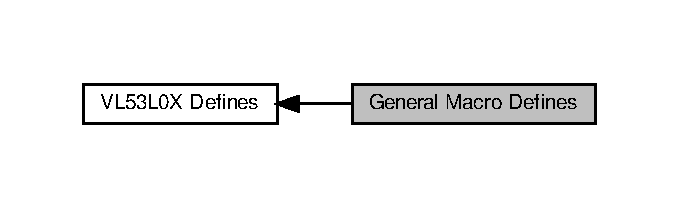
\includegraphics[width=326pt]{group__VL53L0X__define__GeneralMacro__group}
\end{center}
\end{figure}
\subsection*{Macros}
\begin{DoxyCompactItemize}
\item 
\mbox{\Hypertarget{group__VL53L0X__define__GeneralMacro__group_gaf05e77eb0d359a32ee6c83172b3da513}\label{group__VL53L0X__define__GeneralMacro__group_gaf05e77eb0d359a32ee6c83172b3da513}} 
\#define {\bfseries V\+L53\+L0\+X\+\_\+\+S\+E\+T\+P\+A\+R\+A\+M\+E\+T\+E\+R\+F\+I\+E\+LD}(Dev,  field,  value)~\hyperlink{group__VL53L0X__platform__group_ga7d67a50d6fbce3ffdb71b4b3f7cbdf39}{P\+A\+L\+Dev\+Data\+Set}(Dev, Current\+Parameters.\+field, value)
\item 
\mbox{\Hypertarget{group__VL53L0X__define__GeneralMacro__group_ga9b7d953c2ac75a493a51d9e19ab7a33f}\label{group__VL53L0X__define__GeneralMacro__group_ga9b7d953c2ac75a493a51d9e19ab7a33f}} 
\#define {\bfseries V\+L53\+L0\+X\+\_\+\+G\+E\+T\+P\+A\+R\+A\+M\+E\+T\+E\+R\+F\+I\+E\+LD}(Dev,  field,  variable)~variable = \hyperlink{group__VL53L0X__platform__group_ga21f3ef1fbe84f5cf77d989c95f21ad0a}{P\+A\+L\+Dev\+Data\+Get}(Dev, Current\+Parameters).field
\item 
\mbox{\Hypertarget{group__VL53L0X__define__GeneralMacro__group_ga47598a8e8857a13e300f585ea0106892}\label{group__VL53L0X__define__GeneralMacro__group_ga47598a8e8857a13e300f585ea0106892}} 
\#define {\bfseries V\+L53\+L0\+X\+\_\+\+S\+E\+T\+A\+R\+R\+A\+Y\+P\+A\+R\+A\+M\+E\+T\+E\+R\+F\+I\+E\+LD}(Dev,  field,  index,  value)~\hyperlink{group__VL53L0X__platform__group_ga7d67a50d6fbce3ffdb71b4b3f7cbdf39}{P\+A\+L\+Dev\+Data\+Set}(Dev, Current\+Parameters.\+field\mbox{[}index\mbox{]}, value)
\item 
\mbox{\Hypertarget{group__VL53L0X__define__GeneralMacro__group_gaabf50682bc638f1b109333cedbab6bbf}\label{group__VL53L0X__define__GeneralMacro__group_gaabf50682bc638f1b109333cedbab6bbf}} 
\#define {\bfseries V\+L53\+L0\+X\+\_\+\+G\+E\+T\+A\+R\+R\+A\+Y\+P\+A\+R\+A\+M\+E\+T\+E\+R\+F\+I\+E\+LD}(Dev,  field,  index,  variable)~variable = \hyperlink{group__VL53L0X__platform__group_ga21f3ef1fbe84f5cf77d989c95f21ad0a}{P\+A\+L\+Dev\+Data\+Get}(Dev, Current\+Parameters).field\mbox{[}index\mbox{]}
\item 
\mbox{\Hypertarget{group__VL53L0X__define__GeneralMacro__group_gaf99327f12679ada115435e413110eb10}\label{group__VL53L0X__define__GeneralMacro__group_gaf99327f12679ada115435e413110eb10}} 
\#define {\bfseries V\+L53\+L0\+X\+\_\+\+S\+E\+T\+D\+E\+V\+I\+C\+E\+S\+P\+E\+C\+I\+F\+I\+C\+P\+A\+R\+A\+M\+E\+T\+ER}(Dev,  field,  value)~\hyperlink{group__VL53L0X__platform__group_ga7d67a50d6fbce3ffdb71b4b3f7cbdf39}{P\+A\+L\+Dev\+Data\+Set}(Dev, Device\+Specific\+Parameters.\+field, value)
\item 
\mbox{\Hypertarget{group__VL53L0X__define__GeneralMacro__group_ga8179769a43cf26099a37748eb90209ea}\label{group__VL53L0X__define__GeneralMacro__group_ga8179769a43cf26099a37748eb90209ea}} 
\#define {\bfseries V\+L53\+L0\+X\+\_\+\+G\+E\+T\+D\+E\+V\+I\+C\+E\+S\+P\+E\+C\+I\+F\+I\+C\+P\+A\+R\+A\+M\+E\+T\+ER}(Dev,  field)~\hyperlink{group__VL53L0X__platform__group_ga21f3ef1fbe84f5cf77d989c95f21ad0a}{P\+A\+L\+Dev\+Data\+Get}(Dev, Device\+Specific\+Parameters).field
\item 
\mbox{\Hypertarget{group__VL53L0X__define__GeneralMacro__group_ga0409c7cdb1c9cf039c1385761a8267f7}\label{group__VL53L0X__define__GeneralMacro__group_ga0409c7cdb1c9cf039c1385761a8267f7}} 
\#define {\bfseries V\+L53\+L0\+X\+\_\+\+F\+I\+X\+P\+O\+I\+N\+T1616\+T\+O\+F\+I\+X\+P\+O\+I\+N\+T97}(Value)~(\hyperlink{vl53l0x__types_8h_a273cf69d639a59973b6019625df33e30}{uint16\+\_\+t})((Value$>$$>$9)\&0x\+F\+F\+F\+F)
\item 
\mbox{\Hypertarget{group__VL53L0X__define__GeneralMacro__group_ga06b0d6dd3fa847671dcb77c197ead691}\label{group__VL53L0X__define__GeneralMacro__group_ga06b0d6dd3fa847671dcb77c197ead691}} 
\#define {\bfseries V\+L53\+L0\+X\+\_\+\+F\+I\+X\+P\+O\+I\+N\+T97\+T\+O\+F\+I\+X\+P\+O\+I\+N\+T1616}(Value)~(\hyperlink{vl53l0x__types_8h_afb910790161809fc76e1a274a6349384}{Fix\+Point1616\+\_\+t})(Value$<$$<$9)
\item 
\mbox{\Hypertarget{group__VL53L0X__define__GeneralMacro__group_ga5d75b6346e45f0ff8b5cbc8c9bf81a77}\label{group__VL53L0X__define__GeneralMacro__group_ga5d75b6346e45f0ff8b5cbc8c9bf81a77}} 
\#define {\bfseries V\+L53\+L0\+X\+\_\+\+F\+I\+X\+P\+O\+I\+N\+T1616\+T\+O\+F\+I\+X\+P\+O\+I\+N\+T88}(Value)~(\hyperlink{vl53l0x__types_8h_a273cf69d639a59973b6019625df33e30}{uint16\+\_\+t})((Value$>$$>$8)\&0x\+F\+F\+F\+F)
\item 
\mbox{\Hypertarget{group__VL53L0X__define__GeneralMacro__group_ga0d4d860c33534371473b70a8db88dfcf}\label{group__VL53L0X__define__GeneralMacro__group_ga0d4d860c33534371473b70a8db88dfcf}} 
\#define {\bfseries V\+L53\+L0\+X\+\_\+\+F\+I\+X\+P\+O\+I\+N\+T88\+T\+O\+F\+I\+X\+P\+O\+I\+N\+T1616}(Value)~(\hyperlink{vl53l0x__types_8h_afb910790161809fc76e1a274a6349384}{Fix\+Point1616\+\_\+t})(Value$<$$<$8)
\item 
\mbox{\Hypertarget{group__VL53L0X__define__GeneralMacro__group_ga8365bb81241d8e21603f169fcfb7b541}\label{group__VL53L0X__define__GeneralMacro__group_ga8365bb81241d8e21603f169fcfb7b541}} 
\#define {\bfseries V\+L53\+L0\+X\+\_\+\+F\+I\+X\+P\+O\+I\+N\+T1616\+T\+O\+F\+I\+X\+P\+O\+I\+N\+T412}(Value)~(\hyperlink{vl53l0x__types_8h_a273cf69d639a59973b6019625df33e30}{uint16\+\_\+t})((Value$>$$>$4)\&0x\+F\+F\+F\+F)
\item 
\mbox{\Hypertarget{group__VL53L0X__define__GeneralMacro__group_ga5d000734cd704368526f2b1fcfe6130b}\label{group__VL53L0X__define__GeneralMacro__group_ga5d000734cd704368526f2b1fcfe6130b}} 
\#define {\bfseries V\+L53\+L0\+X\+\_\+\+F\+I\+X\+P\+O\+I\+N\+T412\+T\+O\+F\+I\+X\+P\+O\+I\+N\+T1616}(Value)~(\hyperlink{vl53l0x__types_8h_afb910790161809fc76e1a274a6349384}{Fix\+Point1616\+\_\+t})(Value$<$$<$4)
\item 
\mbox{\Hypertarget{group__VL53L0X__define__GeneralMacro__group_ga2bc3eb228078083f39c3a839043fa327}\label{group__VL53L0X__define__GeneralMacro__group_ga2bc3eb228078083f39c3a839043fa327}} 
\#define {\bfseries V\+L53\+L0\+X\+\_\+\+F\+I\+X\+P\+O\+I\+N\+T1616\+T\+O\+F\+I\+X\+P\+O\+I\+N\+T313}(Value)~(\hyperlink{vl53l0x__types_8h_a273cf69d639a59973b6019625df33e30}{uint16\+\_\+t})((Value$>$$>$3)\&0x\+F\+F\+F\+F)
\item 
\mbox{\Hypertarget{group__VL53L0X__define__GeneralMacro__group_ga21742f10715a356bf1ba09fbeb7afd86}\label{group__VL53L0X__define__GeneralMacro__group_ga21742f10715a356bf1ba09fbeb7afd86}} 
\#define {\bfseries V\+L53\+L0\+X\+\_\+\+F\+I\+X\+P\+O\+I\+N\+T313\+T\+O\+F\+I\+X\+P\+O\+I\+N\+T1616}(Value)~(\hyperlink{vl53l0x__types_8h_afb910790161809fc76e1a274a6349384}{Fix\+Point1616\+\_\+t})(Value$<$$<$3)
\item 
\mbox{\Hypertarget{group__VL53L0X__define__GeneralMacro__group_ga2244c6212b240612436b2e1c5a997b9c}\label{group__VL53L0X__define__GeneralMacro__group_ga2244c6212b240612436b2e1c5a997b9c}} 
\#define {\bfseries V\+L53\+L0\+X\+\_\+\+F\+I\+X\+P\+O\+I\+N\+T1616\+T\+O\+F\+I\+X\+P\+O\+I\+N\+T08}(Value)~(\hyperlink{vl53l0x__types_8h_aba7bc1797add20fe3efdf37ced1182c5}{uint8\+\_\+t})((Value$>$$>$8)\&0x00\+F\+F)
\item 
\mbox{\Hypertarget{group__VL53L0X__define__GeneralMacro__group_gac8da31daaf5ee32eb8ce5f524adad30e}\label{group__VL53L0X__define__GeneralMacro__group_gac8da31daaf5ee32eb8ce5f524adad30e}} 
\#define {\bfseries V\+L53\+L0\+X\+\_\+\+F\+I\+X\+P\+O\+I\+N\+T08\+T\+O\+F\+I\+X\+P\+O\+I\+N\+T1616}(Value)~(\hyperlink{vl53l0x__types_8h_afb910790161809fc76e1a274a6349384}{Fix\+Point1616\+\_\+t})(Value$<$$<$8)
\item 
\mbox{\Hypertarget{group__VL53L0X__define__GeneralMacro__group_gaf0fbb69135eec12effce1f330b1adfa1}\label{group__VL53L0X__define__GeneralMacro__group_gaf0fbb69135eec12effce1f330b1adfa1}} 
\#define {\bfseries V\+L53\+L0\+X\+\_\+\+F\+I\+X\+P\+O\+I\+N\+T1616\+T\+O\+F\+I\+X\+P\+O\+I\+N\+T53}(Value)~(\hyperlink{vl53l0x__types_8h_aba7bc1797add20fe3efdf37ced1182c5}{uint8\+\_\+t})((Value$>$$>$13)\&0x00\+F\+F)
\item 
\mbox{\Hypertarget{group__VL53L0X__define__GeneralMacro__group_ga8bf6e9ba87cc29ec573ecb51fbd15ff7}\label{group__VL53L0X__define__GeneralMacro__group_ga8bf6e9ba87cc29ec573ecb51fbd15ff7}} 
\#define {\bfseries V\+L53\+L0\+X\+\_\+\+F\+I\+X\+P\+O\+I\+N\+T53\+T\+O\+F\+I\+X\+P\+O\+I\+N\+T1616}(Value)~(\hyperlink{vl53l0x__types_8h_afb910790161809fc76e1a274a6349384}{Fix\+Point1616\+\_\+t})(Value$<$$<$13)
\item 
\mbox{\Hypertarget{group__VL53L0X__define__GeneralMacro__group_ga7949eb4ea2fa9391005a3ccacff83a19}\label{group__VL53L0X__define__GeneralMacro__group_ga7949eb4ea2fa9391005a3ccacff83a19}} 
\#define {\bfseries V\+L53\+L0\+X\+\_\+\+F\+I\+X\+P\+O\+I\+N\+T1616\+T\+O\+F\+I\+X\+P\+O\+I\+N\+T102}(Value)~(\hyperlink{vl53l0x__types_8h_a273cf69d639a59973b6019625df33e30}{uint16\+\_\+t})((Value$>$$>$14)\&0x0\+F\+F\+F)
\item 
\mbox{\Hypertarget{group__VL53L0X__define__GeneralMacro__group_ga78e08e4ecc017f352d86770d84588ddd}\label{group__VL53L0X__define__GeneralMacro__group_ga78e08e4ecc017f352d86770d84588ddd}} 
\#define {\bfseries V\+L53\+L0\+X\+\_\+\+F\+I\+X\+P\+O\+I\+N\+T102\+T\+O\+F\+I\+X\+P\+O\+I\+N\+T1616}(Value)~(\hyperlink{vl53l0x__types_8h_afb910790161809fc76e1a274a6349384}{Fix\+Point1616\+\_\+t})(Value$<$$<$12)
\item 
\#define {\bfseries V\+L53\+L0\+X\+\_\+\+M\+A\+K\+E\+U\+I\+N\+T16}(lsb,  msb)
\end{DoxyCompactItemize}


\subsection{Detailed Description}
General Macro Defines 

\subsection{Macro Definition Documentation}
\mbox{\Hypertarget{group__VL53L0X__define__GeneralMacro__group_ga6d41b2d37d6121e3b2d2599f1f28311b}\label{group__VL53L0X__define__GeneralMacro__group_ga6d41b2d37d6121e3b2d2599f1f28311b}} 
\index{General Macro Defines@{General Macro Defines}!V\+L53\+L0\+X\+\_\+\+M\+A\+K\+E\+U\+I\+N\+T16@{V\+L53\+L0\+X\+\_\+\+M\+A\+K\+E\+U\+I\+N\+T16}}
\index{V\+L53\+L0\+X\+\_\+\+M\+A\+K\+E\+U\+I\+N\+T16@{V\+L53\+L0\+X\+\_\+\+M\+A\+K\+E\+U\+I\+N\+T16}!General Macro Defines@{General Macro Defines}}
\subsubsection{\texorpdfstring{V\+L53\+L0\+X\+\_\+\+M\+A\+K\+E\+U\+I\+N\+T16}{VL53L0X\_MAKEUINT16}}
{\footnotesize\ttfamily \#define V\+L53\+L0\+X\+\_\+\+M\+A\+K\+E\+U\+I\+N\+T16(\begin{DoxyParamCaption}\item[{}]{lsb,  }\item[{}]{msb }\end{DoxyParamCaption})}

{\bfseries Value\+:}
\begin{DoxyCode}
(\hyperlink{vl53l0x__types_8h_a273cf69d639a59973b6019625df33e30}{uint16\_t})((((\hyperlink{vl53l0x__types_8h_a273cf69d639a59973b6019625df33e30}{uint16\_t})msb)<<8) + \(\backslash\)
        (\hyperlink{vl53l0x__types_8h_a273cf69d639a59973b6019625df33e30}{uint16\_t})lsb)
\end{DoxyCode}

\hypertarget{group__VL53L0X__DevSpecDefines__group}{}\section{V\+L53\+L0X cut1.1 Device Specific Defines}
\label{group__VL53L0X__DevSpecDefines__group}\index{V\+L53\+L0\+X cut1.\+1 Device Specific Defines@{V\+L53\+L0\+X cut1.\+1 Device Specific Defines}}


V\+L53\+L0X cut1.\+1 Device Specific Defines.  


Collaboration diagram for V\+L53\+L0X cut1.1 Device Specific Defines\+:\nopagebreak
\begin{figure}[H]
\begin{center}
\leavevmode
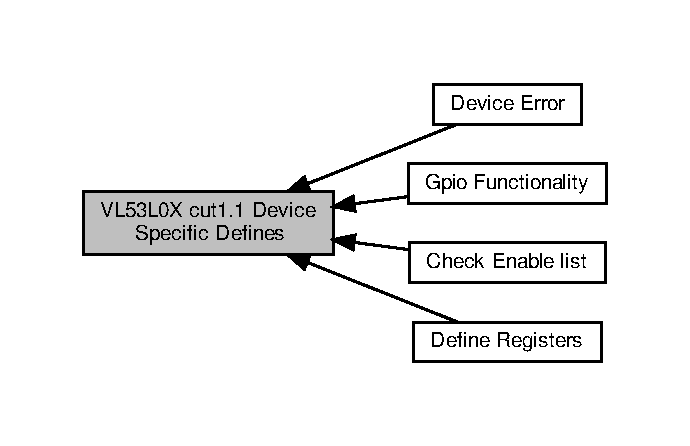
\includegraphics[width=331pt]{group__VL53L0X__DevSpecDefines__group}
\end{center}
\end{figure}
\subsection*{Modules}
\begin{DoxyCompactItemize}
\item 
\hyperlink{group__VL53L0X__DeviceError__group}{Device Error}
\begin{DoxyCompactList}\small\item\em Device Error code. \end{DoxyCompactList}\item 
\hyperlink{group__VL53L0X__CheckEnable__group}{Check Enable list}
\begin{DoxyCompactList}\small\item\em Check Enable code. \end{DoxyCompactList}\item 
\hyperlink{group__VL53L0X__GpioFunctionality__group}{Gpio Functionality}
\begin{DoxyCompactList}\small\item\em Defines the different functionalities for the device G\+P\+I\+O(s) \end{DoxyCompactList}\item 
\hyperlink{group__VL53L0X__DefineRegisters__group}{Define Registers}
\begin{DoxyCompactList}\small\item\em List of all the defined registers. \end{DoxyCompactList}\end{DoxyCompactItemize}


\subsection{Detailed Description}
V\+L53\+L0X cut1.\+1 Device Specific Defines. 

Device specific defines. To be adapted by implementer for the targeted device. 
\hypertarget{group__VL53L0X__DeviceError__group}{}\section{Device Error}
\label{group__VL53L0X__DeviceError__group}\index{Device Error@{Device Error}}


Device Error code.  


Collaboration diagram for Device Error\+:\nopagebreak
\begin{figure}[H]
\begin{center}
\leavevmode
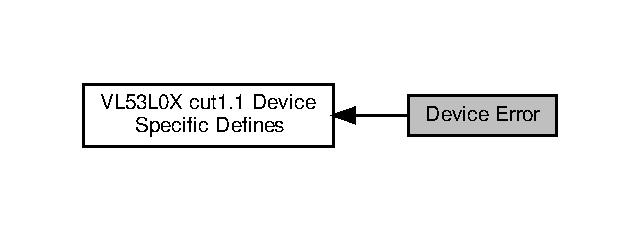
\includegraphics[width=307pt]{group__VL53L0X__DeviceError__group}
\end{center}
\end{figure}
\subsection*{Macros}
\begin{DoxyCompactItemize}
\item 
\#define \hyperlink{group__VL53L0X__DeviceError__group_gada232800eb73d4e8ef6fb2ca506f7030}{V\+L53\+L0\+X\+\_\+\+D\+E\+V\+I\+C\+E\+E\+R\+R\+O\+R\+\_\+\+N\+O\+NE}~((V\+L53\+L0\+X\+\_\+\+Device\+Error) 0)
\item 
\mbox{\Hypertarget{group__VL53L0X__DeviceError__group_ga990b58d47de775fafe1d03e28498ccd8}\label{group__VL53L0X__DeviceError__group_ga990b58d47de775fafe1d03e28498ccd8}} 
\#define {\bfseries V\+L53\+L0\+X\+\_\+\+D\+E\+V\+I\+C\+E\+E\+R\+R\+O\+R\+\_\+\+V\+C\+S\+E\+L\+C\+O\+N\+T\+I\+N\+U\+I\+T\+Y\+T\+E\+S\+T\+F\+A\+I\+L\+U\+RE}~((V\+L53\+L0\+X\+\_\+\+Device\+Error) 1)
\item 
\mbox{\Hypertarget{group__VL53L0X__DeviceError__group_ga59380b9d2d9314d1664f95f043408034}\label{group__VL53L0X__DeviceError__group_ga59380b9d2d9314d1664f95f043408034}} 
\#define {\bfseries V\+L53\+L0\+X\+\_\+\+D\+E\+V\+I\+C\+E\+E\+R\+R\+O\+R\+\_\+\+V\+C\+S\+E\+L\+W\+A\+T\+C\+H\+D\+O\+G\+T\+E\+S\+T\+F\+A\+I\+L\+U\+RE}~((V\+L53\+L0\+X\+\_\+\+Device\+Error) 2)
\item 
\mbox{\Hypertarget{group__VL53L0X__DeviceError__group_ga8da0ee3227f4ec72ff2927c7cdff8cfe}\label{group__VL53L0X__DeviceError__group_ga8da0ee3227f4ec72ff2927c7cdff8cfe}} 
\#define {\bfseries V\+L53\+L0\+X\+\_\+\+D\+E\+V\+I\+C\+E\+E\+R\+R\+O\+R\+\_\+\+N\+O\+V\+H\+V\+V\+A\+L\+U\+E\+F\+O\+U\+ND}~((V\+L53\+L0\+X\+\_\+\+Device\+Error) 3)
\item 
\mbox{\Hypertarget{group__VL53L0X__DeviceError__group_gabfceff1bf6e945a8647c6e980331925c}\label{group__VL53L0X__DeviceError__group_gabfceff1bf6e945a8647c6e980331925c}} 
\#define {\bfseries V\+L53\+L0\+X\+\_\+\+D\+E\+V\+I\+C\+E\+E\+R\+R\+O\+R\+\_\+\+M\+S\+R\+C\+N\+O\+T\+A\+R\+G\+ET}~((V\+L53\+L0\+X\+\_\+\+Device\+Error) 4)
\item 
\mbox{\Hypertarget{group__VL53L0X__DeviceError__group_ga6864aeef5af11cb8b987ca62010643b6}\label{group__VL53L0X__DeviceError__group_ga6864aeef5af11cb8b987ca62010643b6}} 
\#define {\bfseries V\+L53\+L0\+X\+\_\+\+D\+E\+V\+I\+C\+E\+E\+R\+R\+O\+R\+\_\+\+S\+N\+R\+C\+H\+E\+CK}~((V\+L53\+L0\+X\+\_\+\+Device\+Error) 5)
\item 
\mbox{\Hypertarget{group__VL53L0X__DeviceError__group_gaec4009280b2031a81f49131557838001}\label{group__VL53L0X__DeviceError__group_gaec4009280b2031a81f49131557838001}} 
\#define {\bfseries V\+L53\+L0\+X\+\_\+\+D\+E\+V\+I\+C\+E\+E\+R\+R\+O\+R\+\_\+\+R\+A\+N\+G\+E\+P\+H\+A\+S\+E\+C\+H\+E\+CK}~((V\+L53\+L0\+X\+\_\+\+Device\+Error) 6)
\item 
\mbox{\Hypertarget{group__VL53L0X__DeviceError__group_ga8fc4ca53c3c74128f3bdb22627931d13}\label{group__VL53L0X__DeviceError__group_ga8fc4ca53c3c74128f3bdb22627931d13}} 
\#define {\bfseries V\+L53\+L0\+X\+\_\+\+D\+E\+V\+I\+C\+E\+E\+R\+R\+O\+R\+\_\+\+S\+I\+G\+M\+A\+T\+H\+R\+E\+S\+H\+O\+L\+D\+C\+H\+E\+CK}~((V\+L53\+L0\+X\+\_\+\+Device\+Error) 7)
\item 
\mbox{\Hypertarget{group__VL53L0X__DeviceError__group_ga2d2d4a90c3faeaeb70469ea94e9b31ab}\label{group__VL53L0X__DeviceError__group_ga2d2d4a90c3faeaeb70469ea94e9b31ab}} 
\#define {\bfseries V\+L53\+L0\+X\+\_\+\+D\+E\+V\+I\+C\+E\+E\+R\+R\+O\+R\+\_\+\+T\+CC}~((V\+L53\+L0\+X\+\_\+\+Device\+Error) 8)
\item 
\mbox{\Hypertarget{group__VL53L0X__DeviceError__group_ga7029010c1a0a8be3aab1592db712d1ab}\label{group__VL53L0X__DeviceError__group_ga7029010c1a0a8be3aab1592db712d1ab}} 
\#define {\bfseries V\+L53\+L0\+X\+\_\+\+D\+E\+V\+I\+C\+E\+E\+R\+R\+O\+R\+\_\+\+P\+H\+A\+S\+E\+C\+O\+N\+S\+I\+S\+T\+E\+N\+CY}~((V\+L53\+L0\+X\+\_\+\+Device\+Error) 9)
\item 
\mbox{\Hypertarget{group__VL53L0X__DeviceError__group_ga0785518b5293d64efc259aa54417b799}\label{group__VL53L0X__DeviceError__group_ga0785518b5293d64efc259aa54417b799}} 
\#define {\bfseries V\+L53\+L0\+X\+\_\+\+D\+E\+V\+I\+C\+E\+E\+R\+R\+O\+R\+\_\+\+M\+I\+N\+C\+L\+IP}~((V\+L53\+L0\+X\+\_\+\+Device\+Error) 10)
\item 
\mbox{\Hypertarget{group__VL53L0X__DeviceError__group_ga1d304d396d8e3cc52b2f1c6cd5255391}\label{group__VL53L0X__DeviceError__group_ga1d304d396d8e3cc52b2f1c6cd5255391}} 
\#define {\bfseries V\+L53\+L0\+X\+\_\+\+D\+E\+V\+I\+C\+E\+E\+R\+R\+O\+R\+\_\+\+R\+A\+N\+G\+E\+C\+O\+M\+P\+L\+E\+TE}~((V\+L53\+L0\+X\+\_\+\+Device\+Error) 11)
\item 
\mbox{\Hypertarget{group__VL53L0X__DeviceError__group_gaf62080499110dcfce5e394ccb3b7ccfc}\label{group__VL53L0X__DeviceError__group_gaf62080499110dcfce5e394ccb3b7ccfc}} 
\#define {\bfseries V\+L53\+L0\+X\+\_\+\+D\+E\+V\+I\+C\+E\+E\+R\+R\+O\+R\+\_\+\+A\+L\+G\+O\+U\+N\+D\+E\+R\+F\+L\+OW}~((V\+L53\+L0\+X\+\_\+\+Device\+Error) 12)
\item 
\mbox{\Hypertarget{group__VL53L0X__DeviceError__group_ga2fcd5c19bb4d81fa2d84396ab3a07f23}\label{group__VL53L0X__DeviceError__group_ga2fcd5c19bb4d81fa2d84396ab3a07f23}} 
\#define {\bfseries V\+L53\+L0\+X\+\_\+\+D\+E\+V\+I\+C\+E\+E\+R\+R\+O\+R\+\_\+\+A\+L\+G\+O\+O\+V\+E\+R\+F\+L\+OW}~((V\+L53\+L0\+X\+\_\+\+Device\+Error) 13)
\item 
\mbox{\Hypertarget{group__VL53L0X__DeviceError__group_gabe98d58fc965f547d32579c333ed823c}\label{group__VL53L0X__DeviceError__group_gabe98d58fc965f547d32579c333ed823c}} 
\#define {\bfseries V\+L53\+L0\+X\+\_\+\+D\+E\+V\+I\+C\+E\+E\+R\+R\+O\+R\+\_\+\+R\+A\+N\+G\+E\+I\+G\+N\+O\+R\+E\+T\+H\+R\+E\+S\+H\+O\+LD}~((V\+L53\+L0\+X\+\_\+\+Device\+Error) 14)
\end{DoxyCompactItemize}
\subsection*{Typedefs}
\begin{DoxyCompactItemize}
\item 
\mbox{\Hypertarget{group__VL53L0X__DeviceError__group_ga25f8b4de6943ec6f55a0a8319ef7e025}\label{group__VL53L0X__DeviceError__group_ga25f8b4de6943ec6f55a0a8319ef7e025}} 
typedef \hyperlink{vl53l0x__types_8h_aba7bc1797add20fe3efdf37ced1182c5}{uint8\+\_\+t} {\bfseries V\+L53\+L0\+X\+\_\+\+Device\+Error}
\end{DoxyCompactItemize}


\subsection{Detailed Description}
Device Error code. 

This enum is Device specific it should be updated in the implementation Use {\itshape V\+L53\+L0\+X\+\_\+\+Get\+Status\+Error\+String()} to get the string. It is related to Status Register of the Device. 

\subsection{Macro Definition Documentation}
\mbox{\Hypertarget{group__VL53L0X__DeviceError__group_gada232800eb73d4e8ef6fb2ca506f7030}\label{group__VL53L0X__DeviceError__group_gada232800eb73d4e8ef6fb2ca506f7030}} 
\index{Device Error@{Device Error}!V\+L53\+L0\+X\+\_\+\+D\+E\+V\+I\+C\+E\+E\+R\+R\+O\+R\+\_\+\+N\+O\+NE@{V\+L53\+L0\+X\+\_\+\+D\+E\+V\+I\+C\+E\+E\+R\+R\+O\+R\+\_\+\+N\+O\+NE}}
\index{V\+L53\+L0\+X\+\_\+\+D\+E\+V\+I\+C\+E\+E\+R\+R\+O\+R\+\_\+\+N\+O\+NE@{V\+L53\+L0\+X\+\_\+\+D\+E\+V\+I\+C\+E\+E\+R\+R\+O\+R\+\_\+\+N\+O\+NE}!Device Error@{Device Error}}
\subsubsection{\texorpdfstring{V\+L53\+L0\+X\+\_\+\+D\+E\+V\+I\+C\+E\+E\+R\+R\+O\+R\+\_\+\+N\+O\+NE}{VL53L0X\_DEVICEERROR\_NONE}}
{\footnotesize\ttfamily \#define V\+L53\+L0\+X\+\_\+\+D\+E\+V\+I\+C\+E\+E\+R\+R\+O\+R\+\_\+\+N\+O\+NE~((V\+L53\+L0\+X\+\_\+\+Device\+Error) 0)}

0 No\+Error 
\hypertarget{group__VL53L0X__CheckEnable__group}{}\section{Check Enable list}
\label{group__VL53L0X__CheckEnable__group}\index{Check Enable list@{Check Enable list}}


Check Enable code.  


Collaboration diagram for Check Enable list\+:\nopagebreak
\begin{figure}[H]
\begin{center}
\leavevmode
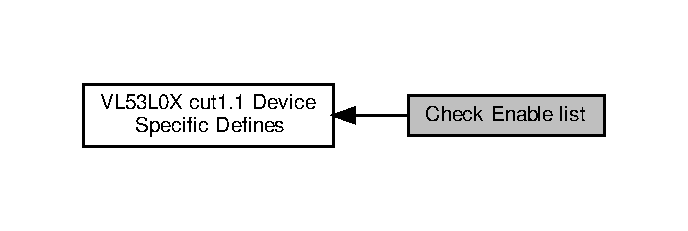
\includegraphics[width=330pt]{group__VL53L0X__CheckEnable__group}
\end{center}
\end{figure}
\subsection*{Macros}
\begin{DoxyCompactItemize}
\item 
\mbox{\Hypertarget{group__VL53L0X__CheckEnable__group_ga2201b410d5221ebe2a6c151bd32f1cd9}\label{group__VL53L0X__CheckEnable__group_ga2201b410d5221ebe2a6c151bd32f1cd9}} 
\#define {\bfseries V\+L53\+L0\+X\+\_\+\+C\+H\+E\+C\+K\+E\+N\+A\+B\+L\+E\+\_\+\+S\+I\+G\+M\+A\+\_\+\+F\+I\+N\+A\+L\+\_\+\+R\+A\+N\+GE}~0
\item 
\mbox{\Hypertarget{group__VL53L0X__CheckEnable__group_ga2cd54f4e61f55a39e6bdb024014dbffd}\label{group__VL53L0X__CheckEnable__group_ga2cd54f4e61f55a39e6bdb024014dbffd}} 
\#define {\bfseries V\+L53\+L0\+X\+\_\+\+C\+H\+E\+C\+K\+E\+N\+A\+B\+L\+E\+\_\+\+S\+I\+G\+N\+A\+L\+\_\+\+R\+A\+T\+E\+\_\+\+F\+I\+N\+A\+L\+\_\+\+R\+A\+N\+GE}~1
\item 
\mbox{\Hypertarget{group__VL53L0X__CheckEnable__group_ga3a8bdb391251ba0706c448b147219020}\label{group__VL53L0X__CheckEnable__group_ga3a8bdb391251ba0706c448b147219020}} 
\#define {\bfseries V\+L53\+L0\+X\+\_\+\+C\+H\+E\+C\+K\+E\+N\+A\+B\+L\+E\+\_\+\+S\+I\+G\+N\+A\+L\+\_\+\+R\+E\+F\+\_\+\+C\+L\+IP}~2
\item 
\mbox{\Hypertarget{group__VL53L0X__CheckEnable__group_ga26fd8247e6738e14fa805c98c96fdbde}\label{group__VL53L0X__CheckEnable__group_ga26fd8247e6738e14fa805c98c96fdbde}} 
\#define {\bfseries V\+L53\+L0\+X\+\_\+\+C\+H\+E\+C\+K\+E\+N\+A\+B\+L\+E\+\_\+\+R\+A\+N\+G\+E\+\_\+\+I\+G\+N\+O\+R\+E\+\_\+\+T\+H\+R\+E\+S\+H\+O\+LD}~3
\item 
\mbox{\Hypertarget{group__VL53L0X__CheckEnable__group_ga801ff9210173264de83628bcf0993885}\label{group__VL53L0X__CheckEnable__group_ga801ff9210173264de83628bcf0993885}} 
\#define {\bfseries V\+L53\+L0\+X\+\_\+\+C\+H\+E\+C\+K\+E\+N\+A\+B\+L\+E\+\_\+\+S\+I\+G\+N\+A\+L\+\_\+\+R\+A\+T\+E\+\_\+\+M\+S\+RC}~4
\item 
\mbox{\Hypertarget{group__VL53L0X__CheckEnable__group_ga71bd7d9eeb02a86282dff820962e3106}\label{group__VL53L0X__CheckEnable__group_ga71bd7d9eeb02a86282dff820962e3106}} 
\#define {\bfseries V\+L53\+L0\+X\+\_\+\+C\+H\+E\+C\+K\+E\+N\+A\+B\+L\+E\+\_\+\+S\+I\+G\+N\+A\+L\+\_\+\+R\+A\+T\+E\+\_\+\+P\+R\+E\+\_\+\+R\+A\+N\+GE}~5
\item 
\mbox{\Hypertarget{group__VL53L0X__CheckEnable__group_ga91e1d823cc96fc1c11e0c9b64247b257}\label{group__VL53L0X__CheckEnable__group_ga91e1d823cc96fc1c11e0c9b64247b257}} 
\#define {\bfseries V\+L53\+L0\+X\+\_\+\+C\+H\+E\+C\+K\+E\+N\+A\+B\+L\+E\+\_\+\+N\+U\+M\+B\+E\+R\+\_\+\+O\+F\+\_\+\+C\+H\+E\+C\+KS}~6
\end{DoxyCompactItemize}


\subsection{Detailed Description}
Check Enable code. 

Define used to specify the Limit\+Check\+Id. Use {\itshape \hyperlink{group__VL53L0X__parameters__group_ga4155c6a50a3eaf215d686759022a68f8}{V\+L53\+L0\+X\+\_\+\+Get\+Limit\+Check\+Info()}} to get the string. 
\hypertarget{group__VL53L0X__GpioFunctionality__group}{}\section{Gpio Functionality}
\label{group__VL53L0X__GpioFunctionality__group}\index{Gpio Functionality@{Gpio Functionality}}


Defines the different functionalities for the device G\+P\+I\+O(s)  


Collaboration diagram for Gpio Functionality\+:\nopagebreak
\begin{figure}[H]
\begin{center}
\leavevmode
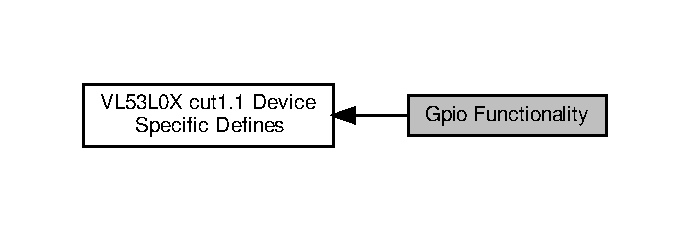
\includegraphics[width=331pt]{group__VL53L0X__GpioFunctionality__group}
\end{center}
\end{figure}
\subsection*{Macros}
\begin{DoxyCompactItemize}
\item 
\#define \hyperlink{group__VL53L0X__GpioFunctionality__group_gafd418cbb738c9910df7ac6a295756bab}{V\+L53\+L0\+X\+\_\+\+G\+P\+I\+O\+F\+U\+N\+C\+T\+I\+O\+N\+A\+L\+I\+T\+Y\+\_\+\+O\+FF}~((V\+L53\+L0\+X\+\_\+\+Gpio\+Functionality)  0)
\item 
\#define \hyperlink{group__VL53L0X__GpioFunctionality__group_ga83eb94bc4301f3b4b23ca38d3d7254a8}{V\+L53\+L0\+X\+\_\+\+G\+P\+I\+O\+F\+U\+N\+C\+T\+I\+O\+N\+A\+L\+I\+T\+Y\+\_\+\+T\+H\+R\+E\+S\+H\+O\+L\+D\+\_\+\+C\+R\+O\+S\+S\+E\+D\+\_\+\+L\+OW}~((V\+L53\+L0\+X\+\_\+\+Gpio\+Functionality)  1)
\item 
\#define \hyperlink{group__VL53L0X__GpioFunctionality__group_gad62d562dde58fb90579a9cdb8730ef4a}{V\+L53\+L0\+X\+\_\+\+G\+P\+I\+O\+F\+U\+N\+C\+T\+I\+O\+N\+A\+L\+I\+T\+Y\+\_\+\+T\+H\+R\+E\+S\+H\+O\+L\+D\+\_\+\+C\+R\+O\+S\+S\+E\+D\+\_\+\+H\+I\+GH}~((V\+L53\+L0\+X\+\_\+\+Gpio\+Functionality)  2)
\item 
\#define \hyperlink{group__VL53L0X__GpioFunctionality__group_gaed6e0c9247a90235c09a7321443c4a54}{V\+L53\+L0\+X\+\_\+\+G\+P\+I\+O\+F\+U\+N\+C\+T\+I\+O\+N\+A\+L\+I\+T\+Y\+\_\+\+T\+H\+R\+E\+S\+H\+O\+L\+D\+\_\+\+C\+R\+O\+S\+S\+E\+D\+\_\+\+O\+UT}~((V\+L53\+L0\+X\+\_\+\+Gpio\+Functionality)  3)
\item 
\#define \hyperlink{group__VL53L0X__GpioFunctionality__group_gaade66f66478f543456a11f854a5bf7de}{V\+L53\+L0\+X\+\_\+\+G\+P\+I\+O\+F\+U\+N\+C\+T\+I\+O\+N\+A\+L\+I\+T\+Y\+\_\+\+N\+E\+W\+\_\+\+M\+E\+A\+S\+U\+R\+E\+\_\+\+R\+E\+A\+DY}~((V\+L53\+L0\+X\+\_\+\+Gpio\+Functionality)  4)
\end{DoxyCompactItemize}
\subsection*{Typedefs}
\begin{DoxyCompactItemize}
\item 
\mbox{\Hypertarget{group__VL53L0X__GpioFunctionality__group_ga19b10d624b1471629e621b60c025b494}\label{group__VL53L0X__GpioFunctionality__group_ga19b10d624b1471629e621b60c025b494}} 
typedef \hyperlink{vl53l0x__types_8h_aba7bc1797add20fe3efdf37ced1182c5}{uint8\+\_\+t} {\bfseries V\+L53\+L0\+X\+\_\+\+Gpio\+Functionality}
\end{DoxyCompactItemize}


\subsection{Detailed Description}
Defines the different functionalities for the device G\+P\+I\+O(s) 



\subsection{Macro Definition Documentation}
\mbox{\Hypertarget{group__VL53L0X__GpioFunctionality__group_gaade66f66478f543456a11f854a5bf7de}\label{group__VL53L0X__GpioFunctionality__group_gaade66f66478f543456a11f854a5bf7de}} 
\index{Gpio Functionality@{Gpio Functionality}!V\+L53\+L0\+X\+\_\+\+G\+P\+I\+O\+F\+U\+N\+C\+T\+I\+O\+N\+A\+L\+I\+T\+Y\+\_\+\+N\+E\+W\+\_\+\+M\+E\+A\+S\+U\+R\+E\+\_\+\+R\+E\+A\+DY@{V\+L53\+L0\+X\+\_\+\+G\+P\+I\+O\+F\+U\+N\+C\+T\+I\+O\+N\+A\+L\+I\+T\+Y\+\_\+\+N\+E\+W\+\_\+\+M\+E\+A\+S\+U\+R\+E\+\_\+\+R\+E\+A\+DY}}
\index{V\+L53\+L0\+X\+\_\+\+G\+P\+I\+O\+F\+U\+N\+C\+T\+I\+O\+N\+A\+L\+I\+T\+Y\+\_\+\+N\+E\+W\+\_\+\+M\+E\+A\+S\+U\+R\+E\+\_\+\+R\+E\+A\+DY@{V\+L53\+L0\+X\+\_\+\+G\+P\+I\+O\+F\+U\+N\+C\+T\+I\+O\+N\+A\+L\+I\+T\+Y\+\_\+\+N\+E\+W\+\_\+\+M\+E\+A\+S\+U\+R\+E\+\_\+\+R\+E\+A\+DY}!Gpio Functionality@{Gpio Functionality}}
\subsubsection{\texorpdfstring{V\+L53\+L0\+X\+\_\+\+G\+P\+I\+O\+F\+U\+N\+C\+T\+I\+O\+N\+A\+L\+I\+T\+Y\+\_\+\+N\+E\+W\+\_\+\+M\+E\+A\+S\+U\+R\+E\+\_\+\+R\+E\+A\+DY}{VL53L0X\_GPIOFUNCTIONALITY\_NEW\_MEASURE\_READY}}
{\footnotesize\ttfamily \#define V\+L53\+L0\+X\+\_\+\+G\+P\+I\+O\+F\+U\+N\+C\+T\+I\+O\+N\+A\+L\+I\+T\+Y\+\_\+\+N\+E\+W\+\_\+\+M\+E\+A\+S\+U\+R\+E\+\_\+\+R\+E\+A\+DY~((V\+L53\+L0\+X\+\_\+\+Gpio\+Functionality)  4)}

New Sample Ready \mbox{\Hypertarget{group__VL53L0X__GpioFunctionality__group_gafd418cbb738c9910df7ac6a295756bab}\label{group__VL53L0X__GpioFunctionality__group_gafd418cbb738c9910df7ac6a295756bab}} 
\index{Gpio Functionality@{Gpio Functionality}!V\+L53\+L0\+X\+\_\+\+G\+P\+I\+O\+F\+U\+N\+C\+T\+I\+O\+N\+A\+L\+I\+T\+Y\+\_\+\+O\+FF@{V\+L53\+L0\+X\+\_\+\+G\+P\+I\+O\+F\+U\+N\+C\+T\+I\+O\+N\+A\+L\+I\+T\+Y\+\_\+\+O\+FF}}
\index{V\+L53\+L0\+X\+\_\+\+G\+P\+I\+O\+F\+U\+N\+C\+T\+I\+O\+N\+A\+L\+I\+T\+Y\+\_\+\+O\+FF@{V\+L53\+L0\+X\+\_\+\+G\+P\+I\+O\+F\+U\+N\+C\+T\+I\+O\+N\+A\+L\+I\+T\+Y\+\_\+\+O\+FF}!Gpio Functionality@{Gpio Functionality}}
\subsubsection{\texorpdfstring{V\+L53\+L0\+X\+\_\+\+G\+P\+I\+O\+F\+U\+N\+C\+T\+I\+O\+N\+A\+L\+I\+T\+Y\+\_\+\+O\+FF}{VL53L0X\_GPIOFUNCTIONALITY\_OFF}}
{\footnotesize\ttfamily \#define V\+L53\+L0\+X\+\_\+\+G\+P\+I\+O\+F\+U\+N\+C\+T\+I\+O\+N\+A\+L\+I\+T\+Y\+\_\+\+O\+FF~((V\+L53\+L0\+X\+\_\+\+Gpio\+Functionality)  0)}

NO Interrupt \mbox{\Hypertarget{group__VL53L0X__GpioFunctionality__group_gad62d562dde58fb90579a9cdb8730ef4a}\label{group__VL53L0X__GpioFunctionality__group_gad62d562dde58fb90579a9cdb8730ef4a}} 
\index{Gpio Functionality@{Gpio Functionality}!V\+L53\+L0\+X\+\_\+\+G\+P\+I\+O\+F\+U\+N\+C\+T\+I\+O\+N\+A\+L\+I\+T\+Y\+\_\+\+T\+H\+R\+E\+S\+H\+O\+L\+D\+\_\+\+C\+R\+O\+S\+S\+E\+D\+\_\+\+H\+I\+GH@{V\+L53\+L0\+X\+\_\+\+G\+P\+I\+O\+F\+U\+N\+C\+T\+I\+O\+N\+A\+L\+I\+T\+Y\+\_\+\+T\+H\+R\+E\+S\+H\+O\+L\+D\+\_\+\+C\+R\+O\+S\+S\+E\+D\+\_\+\+H\+I\+GH}}
\index{V\+L53\+L0\+X\+\_\+\+G\+P\+I\+O\+F\+U\+N\+C\+T\+I\+O\+N\+A\+L\+I\+T\+Y\+\_\+\+T\+H\+R\+E\+S\+H\+O\+L\+D\+\_\+\+C\+R\+O\+S\+S\+E\+D\+\_\+\+H\+I\+GH@{V\+L53\+L0\+X\+\_\+\+G\+P\+I\+O\+F\+U\+N\+C\+T\+I\+O\+N\+A\+L\+I\+T\+Y\+\_\+\+T\+H\+R\+E\+S\+H\+O\+L\+D\+\_\+\+C\+R\+O\+S\+S\+E\+D\+\_\+\+H\+I\+GH}!Gpio Functionality@{Gpio Functionality}}
\subsubsection{\texorpdfstring{V\+L53\+L0\+X\+\_\+\+G\+P\+I\+O\+F\+U\+N\+C\+T\+I\+O\+N\+A\+L\+I\+T\+Y\+\_\+\+T\+H\+R\+E\+S\+H\+O\+L\+D\+\_\+\+C\+R\+O\+S\+S\+E\+D\+\_\+\+H\+I\+GH}{VL53L0X\_GPIOFUNCTIONALITY\_THRESHOLD\_CROSSED\_HIGH}}
{\footnotesize\ttfamily \#define V\+L53\+L0\+X\+\_\+\+G\+P\+I\+O\+F\+U\+N\+C\+T\+I\+O\+N\+A\+L\+I\+T\+Y\+\_\+\+T\+H\+R\+E\+S\+H\+O\+L\+D\+\_\+\+C\+R\+O\+S\+S\+E\+D\+\_\+\+H\+I\+GH~((V\+L53\+L0\+X\+\_\+\+Gpio\+Functionality)  2)}

Level High (value $>$ thresh\+\_\+high) \mbox{\Hypertarget{group__VL53L0X__GpioFunctionality__group_ga83eb94bc4301f3b4b23ca38d3d7254a8}\label{group__VL53L0X__GpioFunctionality__group_ga83eb94bc4301f3b4b23ca38d3d7254a8}} 
\index{Gpio Functionality@{Gpio Functionality}!V\+L53\+L0\+X\+\_\+\+G\+P\+I\+O\+F\+U\+N\+C\+T\+I\+O\+N\+A\+L\+I\+T\+Y\+\_\+\+T\+H\+R\+E\+S\+H\+O\+L\+D\+\_\+\+C\+R\+O\+S\+S\+E\+D\+\_\+\+L\+OW@{V\+L53\+L0\+X\+\_\+\+G\+P\+I\+O\+F\+U\+N\+C\+T\+I\+O\+N\+A\+L\+I\+T\+Y\+\_\+\+T\+H\+R\+E\+S\+H\+O\+L\+D\+\_\+\+C\+R\+O\+S\+S\+E\+D\+\_\+\+L\+OW}}
\index{V\+L53\+L0\+X\+\_\+\+G\+P\+I\+O\+F\+U\+N\+C\+T\+I\+O\+N\+A\+L\+I\+T\+Y\+\_\+\+T\+H\+R\+E\+S\+H\+O\+L\+D\+\_\+\+C\+R\+O\+S\+S\+E\+D\+\_\+\+L\+OW@{V\+L53\+L0\+X\+\_\+\+G\+P\+I\+O\+F\+U\+N\+C\+T\+I\+O\+N\+A\+L\+I\+T\+Y\+\_\+\+T\+H\+R\+E\+S\+H\+O\+L\+D\+\_\+\+C\+R\+O\+S\+S\+E\+D\+\_\+\+L\+OW}!Gpio Functionality@{Gpio Functionality}}
\subsubsection{\texorpdfstring{V\+L53\+L0\+X\+\_\+\+G\+P\+I\+O\+F\+U\+N\+C\+T\+I\+O\+N\+A\+L\+I\+T\+Y\+\_\+\+T\+H\+R\+E\+S\+H\+O\+L\+D\+\_\+\+C\+R\+O\+S\+S\+E\+D\+\_\+\+L\+OW}{VL53L0X\_GPIOFUNCTIONALITY\_THRESHOLD\_CROSSED\_LOW}}
{\footnotesize\ttfamily \#define V\+L53\+L0\+X\+\_\+\+G\+P\+I\+O\+F\+U\+N\+C\+T\+I\+O\+N\+A\+L\+I\+T\+Y\+\_\+\+T\+H\+R\+E\+S\+H\+O\+L\+D\+\_\+\+C\+R\+O\+S\+S\+E\+D\+\_\+\+L\+OW~((V\+L53\+L0\+X\+\_\+\+Gpio\+Functionality)  1)}

Level Low (value $<$ thresh\+\_\+low) \mbox{\Hypertarget{group__VL53L0X__GpioFunctionality__group_gaed6e0c9247a90235c09a7321443c4a54}\label{group__VL53L0X__GpioFunctionality__group_gaed6e0c9247a90235c09a7321443c4a54}} 
\index{Gpio Functionality@{Gpio Functionality}!V\+L53\+L0\+X\+\_\+\+G\+P\+I\+O\+F\+U\+N\+C\+T\+I\+O\+N\+A\+L\+I\+T\+Y\+\_\+\+T\+H\+R\+E\+S\+H\+O\+L\+D\+\_\+\+C\+R\+O\+S\+S\+E\+D\+\_\+\+O\+UT@{V\+L53\+L0\+X\+\_\+\+G\+P\+I\+O\+F\+U\+N\+C\+T\+I\+O\+N\+A\+L\+I\+T\+Y\+\_\+\+T\+H\+R\+E\+S\+H\+O\+L\+D\+\_\+\+C\+R\+O\+S\+S\+E\+D\+\_\+\+O\+UT}}
\index{V\+L53\+L0\+X\+\_\+\+G\+P\+I\+O\+F\+U\+N\+C\+T\+I\+O\+N\+A\+L\+I\+T\+Y\+\_\+\+T\+H\+R\+E\+S\+H\+O\+L\+D\+\_\+\+C\+R\+O\+S\+S\+E\+D\+\_\+\+O\+UT@{V\+L53\+L0\+X\+\_\+\+G\+P\+I\+O\+F\+U\+N\+C\+T\+I\+O\+N\+A\+L\+I\+T\+Y\+\_\+\+T\+H\+R\+E\+S\+H\+O\+L\+D\+\_\+\+C\+R\+O\+S\+S\+E\+D\+\_\+\+O\+UT}!Gpio Functionality@{Gpio Functionality}}
\subsubsection{\texorpdfstring{V\+L53\+L0\+X\+\_\+\+G\+P\+I\+O\+F\+U\+N\+C\+T\+I\+O\+N\+A\+L\+I\+T\+Y\+\_\+\+T\+H\+R\+E\+S\+H\+O\+L\+D\+\_\+\+C\+R\+O\+S\+S\+E\+D\+\_\+\+O\+UT}{VL53L0X\_GPIOFUNCTIONALITY\_THRESHOLD\_CROSSED\_OUT}}
{\footnotesize\ttfamily \#define V\+L53\+L0\+X\+\_\+\+G\+P\+I\+O\+F\+U\+N\+C\+T\+I\+O\+N\+A\+L\+I\+T\+Y\+\_\+\+T\+H\+R\+E\+S\+H\+O\+L\+D\+\_\+\+C\+R\+O\+S\+S\+E\+D\+\_\+\+O\+UT~((V\+L53\+L0\+X\+\_\+\+Gpio\+Functionality)  3)}

Out Of Window (value $<$ thresh\+\_\+low OR value $>$ thresh\+\_\+high) 
\hypertarget{group__VL53L0X__DefineRegisters__group}{}\section{Define Registers}
\label{group__VL53L0X__DefineRegisters__group}\index{Define Registers@{Define Registers}}


List of all the defined registers.  


Collaboration diagram for Define Registers\+:\nopagebreak
\begin{figure}[H]
\begin{center}
\leavevmode
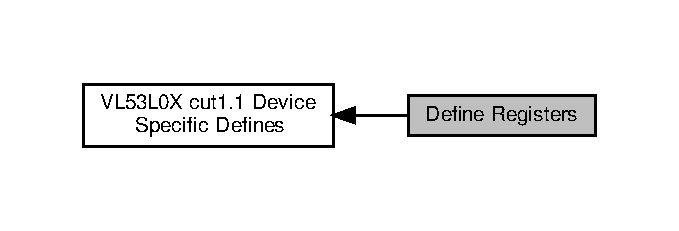
\includegraphics[width=326pt]{group__VL53L0X__DefineRegisters__group}
\end{center}
\end{figure}
\subsection*{Macros}
\begin{DoxyCompactItemize}
\item 
\mbox{\Hypertarget{group__VL53L0X__DefineRegisters__group_ga3dca7e5623fb6fae463a6bc19a2ce689}\label{group__VL53L0X__DefineRegisters__group_ga3dca7e5623fb6fae463a6bc19a2ce689}} 
\#define {\bfseries V\+L53\+L0\+X\+\_\+\+R\+E\+G\+\_\+\+S\+Y\+S\+R\+A\+N\+G\+E\+\_\+\+S\+T\+A\+RT}~0x000
\item 
\#define \hyperlink{group__VL53L0X__DefineRegisters__group_ga8f96d0313124692cef590651600655f6}{V\+L53\+L0\+X\+\_\+\+R\+E\+G\+\_\+\+S\+Y\+S\+R\+A\+N\+G\+E\+\_\+\+M\+O\+D\+E\+\_\+\+M\+A\+SK}~0x0F
\item 
\#define \hyperlink{group__VL53L0X__DefineRegisters__group_ga8022c1d5603bd28dda20d5f6b1b081d5}{V\+L53\+L0\+X\+\_\+\+R\+E\+G\+\_\+\+S\+Y\+S\+R\+A\+N\+G\+E\+\_\+\+M\+O\+D\+E\+\_\+\+S\+T\+A\+R\+T\+\_\+\+S\+T\+OP}~0x01
\item 
\#define \hyperlink{group__VL53L0X__DefineRegisters__group_ga9349d500808730eb4ac139b894898d08}{V\+L53\+L0\+X\+\_\+\+R\+E\+G\+\_\+\+S\+Y\+S\+R\+A\+N\+G\+E\+\_\+\+M\+O\+D\+E\+\_\+\+S\+I\+N\+G\+L\+E\+S\+H\+OT}~0x00
\item 
\#define \hyperlink{group__VL53L0X__DefineRegisters__group_gade8dcdeff5eaca6ab53ca568691bd075}{V\+L53\+L0\+X\+\_\+\+R\+E\+G\+\_\+\+S\+Y\+S\+R\+A\+N\+G\+E\+\_\+\+M\+O\+D\+E\+\_\+\+B\+A\+C\+K\+T\+O\+B\+A\+CK}~0x02
\item 
\#define \hyperlink{group__VL53L0X__DefineRegisters__group_gad492a257e53abe0de3418f5cb337c365}{V\+L53\+L0\+X\+\_\+\+R\+E\+G\+\_\+\+S\+Y\+S\+R\+A\+N\+G\+E\+\_\+\+M\+O\+D\+E\+\_\+\+T\+I\+M\+ED}~0x04
\item 
\#define \hyperlink{group__VL53L0X__DefineRegisters__group_ga0c3b739423d12da8c21ca4bd6f25608c}{V\+L53\+L0\+X\+\_\+\+R\+E\+G\+\_\+\+S\+Y\+S\+R\+A\+N\+G\+E\+\_\+\+M\+O\+D\+E\+\_\+\+H\+I\+S\+T\+O\+G\+R\+AM}~0x08
\item 
\mbox{\Hypertarget{group__VL53L0X__DefineRegisters__group_ga0f30ccd52696614900824d796374ee05}\label{group__VL53L0X__DefineRegisters__group_ga0f30ccd52696614900824d796374ee05}} 
\#define {\bfseries V\+L53\+L0\+X\+\_\+\+R\+E\+G\+\_\+\+S\+Y\+S\+T\+E\+M\+\_\+\+T\+H\+R\+E\+S\+H\+\_\+\+H\+I\+GH}~0x000C
\item 
\mbox{\Hypertarget{group__VL53L0X__DefineRegisters__group_gacb26eb1b499023ab3a5c551d751445f8}\label{group__VL53L0X__DefineRegisters__group_gacb26eb1b499023ab3a5c551d751445f8}} 
\#define {\bfseries V\+L53\+L0\+X\+\_\+\+R\+E\+G\+\_\+\+S\+Y\+S\+T\+E\+M\+\_\+\+T\+H\+R\+E\+S\+H\+\_\+\+L\+OW}~0x000E
\item 
\mbox{\Hypertarget{group__VL53L0X__DefineRegisters__group_gadd8d9d1aa7ca05d809fa0c1dadf3643a}\label{group__VL53L0X__DefineRegisters__group_gadd8d9d1aa7ca05d809fa0c1dadf3643a}} 
\#define {\bfseries V\+L53\+L0\+X\+\_\+\+R\+E\+G\+\_\+\+S\+Y\+S\+T\+E\+M\+\_\+\+S\+E\+Q\+U\+E\+N\+C\+E\+\_\+\+C\+O\+N\+F\+IG}~0x0001
\item 
\mbox{\Hypertarget{group__VL53L0X__DefineRegisters__group_ga205cd5e08da045ed2c4a5dac6f20bebe}\label{group__VL53L0X__DefineRegisters__group_ga205cd5e08da045ed2c4a5dac6f20bebe}} 
\#define {\bfseries V\+L53\+L0\+X\+\_\+\+R\+E\+G\+\_\+\+S\+Y\+S\+T\+E\+M\+\_\+\+R\+A\+N\+G\+E\+\_\+\+C\+O\+N\+F\+IG}~0x0009
\item 
\mbox{\Hypertarget{group__VL53L0X__DefineRegisters__group_gac8a684ca2897371bf74e453600a3ecd1}\label{group__VL53L0X__DefineRegisters__group_gac8a684ca2897371bf74e453600a3ecd1}} 
\#define {\bfseries V\+L53\+L0\+X\+\_\+\+R\+E\+G\+\_\+\+S\+Y\+S\+T\+E\+M\+\_\+\+I\+N\+T\+E\+R\+M\+E\+A\+S\+U\+R\+E\+M\+E\+N\+T\+\_\+\+P\+E\+R\+I\+OD}~0x0004
\item 
\mbox{\Hypertarget{group__VL53L0X__DefineRegisters__group_gae7162490d657797de685d2bf2dc59918}\label{group__VL53L0X__DefineRegisters__group_gae7162490d657797de685d2bf2dc59918}} 
\#define {\bfseries V\+L53\+L0\+X\+\_\+\+R\+E\+G\+\_\+\+S\+Y\+S\+T\+E\+M\+\_\+\+I\+N\+T\+E\+R\+R\+U\+P\+T\+\_\+\+C\+O\+N\+F\+I\+G\+\_\+\+G\+P\+IO}~0x000A
\item 
\mbox{\Hypertarget{group__VL53L0X__DefineRegisters__group_ga8341867e76337cc63a8d9489df30832a}\label{group__VL53L0X__DefineRegisters__group_ga8341867e76337cc63a8d9489df30832a}} 
\#define {\bfseries V\+L53\+L0\+X\+\_\+\+R\+E\+G\+\_\+\+S\+Y\+S\+T\+E\+M\+\_\+\+I\+N\+T\+E\+R\+R\+U\+P\+T\+\_\+\+G\+P\+I\+O\+\_\+\+D\+I\+S\+A\+B\+L\+ED}~0x00
\item 
\mbox{\Hypertarget{group__VL53L0X__DefineRegisters__group_gad003aff8dc5b8ca75a373151bd0b3029}\label{group__VL53L0X__DefineRegisters__group_gad003aff8dc5b8ca75a373151bd0b3029}} 
\#define {\bfseries V\+L53\+L0\+X\+\_\+\+R\+E\+G\+\_\+\+S\+Y\+S\+T\+E\+M\+\_\+\+I\+N\+T\+E\+R\+R\+U\+P\+T\+\_\+\+G\+P\+I\+O\+\_\+\+L\+E\+V\+E\+L\+\_\+\+L\+OW}~0x01
\item 
\mbox{\Hypertarget{group__VL53L0X__DefineRegisters__group_ga104dec5ebba6c67ac81009a768a4b789}\label{group__VL53L0X__DefineRegisters__group_ga104dec5ebba6c67ac81009a768a4b789}} 
\#define {\bfseries V\+L53\+L0\+X\+\_\+\+R\+E\+G\+\_\+\+S\+Y\+S\+T\+E\+M\+\_\+\+I\+N\+T\+E\+R\+R\+U\+P\+T\+\_\+\+G\+P\+I\+O\+\_\+\+L\+E\+V\+E\+L\+\_\+\+H\+I\+GH}~0x02
\item 
\mbox{\Hypertarget{group__VL53L0X__DefineRegisters__group_ga84466f853b4b005accfd4880c219e963}\label{group__VL53L0X__DefineRegisters__group_ga84466f853b4b005accfd4880c219e963}} 
\#define {\bfseries V\+L53\+L0\+X\+\_\+\+R\+E\+G\+\_\+\+S\+Y\+S\+T\+E\+M\+\_\+\+I\+N\+T\+E\+R\+R\+U\+P\+T\+\_\+\+G\+P\+I\+O\+\_\+\+O\+U\+T\+\_\+\+O\+F\+\_\+\+W\+I\+N\+D\+OW}~0x03
\item 
\mbox{\Hypertarget{group__VL53L0X__DefineRegisters__group_gac494308aafc7f7a3c07e9dfd1776dae1}\label{group__VL53L0X__DefineRegisters__group_gac494308aafc7f7a3c07e9dfd1776dae1}} 
\#define {\bfseries V\+L53\+L0\+X\+\_\+\+R\+E\+G\+\_\+\+S\+Y\+S\+T\+E\+M\+\_\+\+I\+N\+T\+E\+R\+R\+U\+P\+T\+\_\+\+G\+P\+I\+O\+\_\+\+N\+E\+W\+\_\+\+S\+A\+M\+P\+L\+E\+\_\+\+R\+E\+A\+DY}~0x04
\item 
\mbox{\Hypertarget{group__VL53L0X__DefineRegisters__group_gaeb245edc08b44ccb9ffceb3a661dee54}\label{group__VL53L0X__DefineRegisters__group_gaeb245edc08b44ccb9ffceb3a661dee54}} 
\#define {\bfseries V\+L53\+L0\+X\+\_\+\+R\+E\+G\+\_\+\+G\+P\+I\+O\+\_\+\+H\+V\+\_\+\+M\+U\+X\+\_\+\+A\+C\+T\+I\+V\+E\+\_\+\+H\+I\+GH}~0x0084
\item 
\mbox{\Hypertarget{group__VL53L0X__DefineRegisters__group_gabb9c3a1aa62ce43de97229eb083f63e6}\label{group__VL53L0X__DefineRegisters__group_gabb9c3a1aa62ce43de97229eb083f63e6}} 
\#define {\bfseries V\+L53\+L0\+X\+\_\+\+R\+E\+G\+\_\+\+S\+Y\+S\+T\+E\+M\+\_\+\+I\+N\+T\+E\+R\+R\+U\+P\+T\+\_\+\+C\+L\+E\+AR}~0x000B
\item 
\mbox{\Hypertarget{group__VL53L0X__DefineRegisters__group_gafd468bf606197a89503bfa69533c46ae}\label{group__VL53L0X__DefineRegisters__group_gafd468bf606197a89503bfa69533c46ae}} 
\#define {\bfseries V\+L53\+L0\+X\+\_\+\+R\+E\+G\+\_\+\+R\+E\+S\+U\+L\+T\+\_\+\+I\+N\+T\+E\+R\+R\+U\+P\+T\+\_\+\+S\+T\+A\+T\+US}~0x0013
\item 
\mbox{\Hypertarget{group__VL53L0X__DefineRegisters__group_gae1c3e69963f637d139084984c869c23c}\label{group__VL53L0X__DefineRegisters__group_gae1c3e69963f637d139084984c869c23c}} 
\#define {\bfseries V\+L53\+L0\+X\+\_\+\+R\+E\+G\+\_\+\+R\+E\+S\+U\+L\+T\+\_\+\+R\+A\+N\+G\+E\+\_\+\+S\+T\+A\+T\+US}~0x0014
\item 
\mbox{\Hypertarget{group__VL53L0X__DefineRegisters__group_ga5ed62d33e4740d65050f7129975a59ac}\label{group__VL53L0X__DefineRegisters__group_ga5ed62d33e4740d65050f7129975a59ac}} 
\#define {\bfseries V\+L53\+L0\+X\+\_\+\+R\+E\+G\+\_\+\+R\+E\+S\+U\+L\+T\+\_\+\+C\+O\+R\+E\+\_\+\+P\+A\+GE}~1
\item 
\mbox{\Hypertarget{group__VL53L0X__DefineRegisters__group_ga13691b09276bccaf8d666717ed8be5c3}\label{group__VL53L0X__DefineRegisters__group_ga13691b09276bccaf8d666717ed8be5c3}} 
\#define {\bfseries V\+L53\+L0\+X\+\_\+\+R\+E\+G\+\_\+\+R\+E\+S\+U\+L\+T\+\_\+\+C\+O\+R\+E\+\_\+\+A\+M\+B\+I\+E\+N\+T\+\_\+\+W\+I\+N\+D\+O\+W\+\_\+\+E\+V\+E\+N\+T\+S\+\_\+\+R\+TN}~0x00\+BC
\item 
\mbox{\Hypertarget{group__VL53L0X__DefineRegisters__group_ga12d588fa642691da2149e7e6b2d40a40}\label{group__VL53L0X__DefineRegisters__group_ga12d588fa642691da2149e7e6b2d40a40}} 
\#define {\bfseries V\+L53\+L0\+X\+\_\+\+R\+E\+G\+\_\+\+R\+E\+S\+U\+L\+T\+\_\+\+C\+O\+R\+E\+\_\+\+R\+A\+N\+G\+I\+N\+G\+\_\+\+T\+O\+T\+A\+L\+\_\+\+E\+V\+E\+N\+T\+S\+\_\+\+R\+TN}~0x00\+C0
\item 
\mbox{\Hypertarget{group__VL53L0X__DefineRegisters__group_gad800373257e5566cc7bbc518fb2f9c9d}\label{group__VL53L0X__DefineRegisters__group_gad800373257e5566cc7bbc518fb2f9c9d}} 
\#define {\bfseries V\+L53\+L0\+X\+\_\+\+R\+E\+G\+\_\+\+R\+E\+S\+U\+L\+T\+\_\+\+C\+O\+R\+E\+\_\+\+A\+M\+B\+I\+E\+N\+T\+\_\+\+W\+I\+N\+D\+O\+W\+\_\+\+E\+V\+E\+N\+T\+S\+\_\+\+R\+EF}~0x00\+D0
\item 
\mbox{\Hypertarget{group__VL53L0X__DefineRegisters__group_ga0ef0fd15d39693e57e0359c3772f0ce4}\label{group__VL53L0X__DefineRegisters__group_ga0ef0fd15d39693e57e0359c3772f0ce4}} 
\#define {\bfseries V\+L53\+L0\+X\+\_\+\+R\+E\+G\+\_\+\+R\+E\+S\+U\+L\+T\+\_\+\+C\+O\+R\+E\+\_\+\+R\+A\+N\+G\+I\+N\+G\+\_\+\+T\+O\+T\+A\+L\+\_\+\+E\+V\+E\+N\+T\+S\+\_\+\+R\+EF}~0x00\+D4
\item 
\mbox{\Hypertarget{group__VL53L0X__DefineRegisters__group_ga5e6507db3533c665dacc5f54c595e3fb}\label{group__VL53L0X__DefineRegisters__group_ga5e6507db3533c665dacc5f54c595e3fb}} 
\#define {\bfseries V\+L53\+L0\+X\+\_\+\+R\+E\+G\+\_\+\+R\+E\+S\+U\+L\+T\+\_\+\+P\+E\+A\+K\+\_\+\+S\+I\+G\+N\+A\+L\+\_\+\+R\+A\+T\+E\+\_\+\+R\+EF}~0x00\+B6
\item 
\mbox{\Hypertarget{group__VL53L0X__DefineRegisters__group_ga4a57a8f4f251b26583074905e614bcaf}\label{group__VL53L0X__DefineRegisters__group_ga4a57a8f4f251b26583074905e614bcaf}} 
\#define {\bfseries V\+L53\+L0\+X\+\_\+\+R\+E\+G\+\_\+\+A\+L\+G\+O\+\_\+\+P\+A\+R\+T\+\_\+\+T\+O\+\_\+\+P\+A\+R\+T\+\_\+\+R\+A\+N\+G\+E\+\_\+\+O\+F\+F\+S\+E\+T\+\_\+\+MM}~0x0028
\item 
\mbox{\Hypertarget{group__VL53L0X__DefineRegisters__group_ga1782cce453f7858909d744eb5ef7d003}\label{group__VL53L0X__DefineRegisters__group_ga1782cce453f7858909d744eb5ef7d003}} 
\#define {\bfseries V\+L53\+L0\+X\+\_\+\+R\+E\+G\+\_\+\+I2\+C\+\_\+\+S\+L\+A\+V\+E\+\_\+\+D\+E\+V\+I\+C\+E\+\_\+\+A\+D\+D\+R\+E\+SS}~0x008a
\item 
\mbox{\Hypertarget{group__VL53L0X__DefineRegisters__group_ga136bdf3400372259d9165a8a2d85eb49}\label{group__VL53L0X__DefineRegisters__group_ga136bdf3400372259d9165a8a2d85eb49}} 
\#define {\bfseries V\+L53\+L0\+X\+\_\+\+R\+E\+G\+\_\+\+M\+S\+R\+C\+\_\+\+C\+O\+N\+F\+I\+G\+\_\+\+C\+O\+N\+T\+R\+OL}~0x0060
\item 
\mbox{\Hypertarget{group__VL53L0X__DefineRegisters__group_ga4288661e82b735fddf1b2b512d242d4d}\label{group__VL53L0X__DefineRegisters__group_ga4288661e82b735fddf1b2b512d242d4d}} 
\#define {\bfseries V\+L53\+L0\+X\+\_\+\+R\+E\+G\+\_\+\+P\+R\+E\+\_\+\+R\+A\+N\+G\+E\+\_\+\+C\+O\+N\+F\+I\+G\+\_\+\+M\+I\+N\+\_\+\+S\+NR}~0\+X0027
\item 
\mbox{\Hypertarget{group__VL53L0X__DefineRegisters__group_ga6132c4f4352120efcba0296c03a09b6b}\label{group__VL53L0X__DefineRegisters__group_ga6132c4f4352120efcba0296c03a09b6b}} 
\#define {\bfseries V\+L53\+L0\+X\+\_\+\+R\+E\+G\+\_\+\+P\+R\+E\+\_\+\+R\+A\+N\+G\+E\+\_\+\+C\+O\+N\+F\+I\+G\+\_\+\+V\+A\+L\+I\+D\+\_\+\+P\+H\+A\+S\+E\+\_\+\+L\+OW}~0x0056
\item 
\mbox{\Hypertarget{group__VL53L0X__DefineRegisters__group_gaf62cc73a306bc0fa69ed4690952b0064}\label{group__VL53L0X__DefineRegisters__group_gaf62cc73a306bc0fa69ed4690952b0064}} 
\#define {\bfseries V\+L53\+L0\+X\+\_\+\+R\+E\+G\+\_\+\+P\+R\+E\+\_\+\+R\+A\+N\+G\+E\+\_\+\+C\+O\+N\+F\+I\+G\+\_\+\+V\+A\+L\+I\+D\+\_\+\+P\+H\+A\+S\+E\+\_\+\+H\+I\+GH}~0x0057
\item 
\mbox{\Hypertarget{group__VL53L0X__DefineRegisters__group_gad0af40dfad234de676ea20941998b486}\label{group__VL53L0X__DefineRegisters__group_gad0af40dfad234de676ea20941998b486}} 
\#define {\bfseries V\+L53\+L0\+X\+\_\+\+R\+E\+G\+\_\+\+P\+R\+E\+\_\+\+R\+A\+N\+G\+E\+\_\+\+M\+I\+N\+\_\+\+C\+O\+U\+N\+T\+\_\+\+R\+A\+T\+E\+\_\+\+R\+T\+N\+\_\+\+L\+I\+M\+IT}~0x0064
\item 
\mbox{\Hypertarget{group__VL53L0X__DefineRegisters__group_ga23391c8e510f910a5caecf48713cc1a7}\label{group__VL53L0X__DefineRegisters__group_ga23391c8e510f910a5caecf48713cc1a7}} 
\#define {\bfseries V\+L53\+L0\+X\+\_\+\+R\+E\+G\+\_\+\+F\+I\+N\+A\+L\+\_\+\+R\+A\+N\+G\+E\+\_\+\+C\+O\+N\+F\+I\+G\+\_\+\+M\+I\+N\+\_\+\+S\+NR}~0\+X0067
\item 
\mbox{\Hypertarget{group__VL53L0X__DefineRegisters__group_gabe44b1496fe8eefdaf477cba2e5964be}\label{group__VL53L0X__DefineRegisters__group_gabe44b1496fe8eefdaf477cba2e5964be}} 
\#define {\bfseries V\+L53\+L0\+X\+\_\+\+R\+E\+G\+\_\+\+F\+I\+N\+A\+L\+\_\+\+R\+A\+N\+G\+E\+\_\+\+C\+O\+N\+F\+I\+G\+\_\+\+V\+A\+L\+I\+D\+\_\+\+P\+H\+A\+S\+E\+\_\+\+L\+OW}~0x0047
\item 
\mbox{\Hypertarget{group__VL53L0X__DefineRegisters__group_ga78de2e1eff30cf5524ecb8e7c5872ec8}\label{group__VL53L0X__DefineRegisters__group_ga78de2e1eff30cf5524ecb8e7c5872ec8}} 
\#define {\bfseries V\+L53\+L0\+X\+\_\+\+R\+E\+G\+\_\+\+F\+I\+N\+A\+L\+\_\+\+R\+A\+N\+G\+E\+\_\+\+C\+O\+N\+F\+I\+G\+\_\+\+V\+A\+L\+I\+D\+\_\+\+P\+H\+A\+S\+E\+\_\+\+H\+I\+GH}~0x0048
\item 
\mbox{\Hypertarget{group__VL53L0X__DefineRegisters__group_ga213342203509c20850a6d4da2c1a7623}\label{group__VL53L0X__DefineRegisters__group_ga213342203509c20850a6d4da2c1a7623}} 
\#define {\bfseries V\+L53\+L0\+X\+\_\+\+R\+E\+G\+\_\+\+F\+I\+N\+A\+L\+\_\+\+R\+A\+N\+G\+E\+\_\+\+C\+O\+N\+F\+I\+G\+\_\+\+M\+I\+N\+\_\+\+C\+O\+U\+N\+T\+\_\+\+R\+A\+T\+E\+\_\+\+R\+T\+N\+\_\+\+L\+I\+M\+IT}~0x0044
\item 
\mbox{\Hypertarget{group__VL53L0X__DefineRegisters__group_ga058e412f106a41a50c1197b524d6c8b5}\label{group__VL53L0X__DefineRegisters__group_ga058e412f106a41a50c1197b524d6c8b5}} 
\#define {\bfseries V\+L53\+L0\+X\+\_\+\+R\+E\+G\+\_\+\+P\+R\+E\+\_\+\+R\+A\+N\+G\+E\+\_\+\+C\+O\+N\+F\+I\+G\+\_\+\+S\+I\+G\+M\+A\+\_\+\+T\+H\+R\+E\+S\+H\+\_\+\+HI}~0\+X0061
\item 
\mbox{\Hypertarget{group__VL53L0X__DefineRegisters__group_ga510287573886507b682549c4119130d2}\label{group__VL53L0X__DefineRegisters__group_ga510287573886507b682549c4119130d2}} 
\#define {\bfseries V\+L53\+L0\+X\+\_\+\+R\+E\+G\+\_\+\+P\+R\+E\+\_\+\+R\+A\+N\+G\+E\+\_\+\+C\+O\+N\+F\+I\+G\+\_\+\+S\+I\+G\+M\+A\+\_\+\+T\+H\+R\+E\+S\+H\+\_\+\+LO}~0\+X0062
\item 
\mbox{\Hypertarget{group__VL53L0X__DefineRegisters__group_ga07f2f6af1daf22f551b2d10fce8709f2}\label{group__VL53L0X__DefineRegisters__group_ga07f2f6af1daf22f551b2d10fce8709f2}} 
\#define {\bfseries V\+L53\+L0\+X\+\_\+\+R\+E\+G\+\_\+\+P\+R\+E\+\_\+\+R\+A\+N\+G\+E\+\_\+\+C\+O\+N\+F\+I\+G\+\_\+\+V\+C\+S\+E\+L\+\_\+\+P\+E\+R\+I\+OD}~0x0050
\item 
\mbox{\Hypertarget{group__VL53L0X__DefineRegisters__group_ga399c03cf46210a004e2e160aeaf69fee}\label{group__VL53L0X__DefineRegisters__group_ga399c03cf46210a004e2e160aeaf69fee}} 
\#define {\bfseries V\+L53\+L0\+X\+\_\+\+R\+E\+G\+\_\+\+P\+R\+E\+\_\+\+R\+A\+N\+G\+E\+\_\+\+C\+O\+N\+F\+I\+G\+\_\+\+T\+I\+M\+E\+O\+U\+T\+\_\+\+M\+A\+C\+R\+O\+P\+\_\+\+HI}~0x0051
\item 
\mbox{\Hypertarget{group__VL53L0X__DefineRegisters__group_gafc8ac6383b221b1fb7cc2ed0f8988e98}\label{group__VL53L0X__DefineRegisters__group_gafc8ac6383b221b1fb7cc2ed0f8988e98}} 
\#define {\bfseries V\+L53\+L0\+X\+\_\+\+R\+E\+G\+\_\+\+P\+R\+E\+\_\+\+R\+A\+N\+G\+E\+\_\+\+C\+O\+N\+F\+I\+G\+\_\+\+T\+I\+M\+E\+O\+U\+T\+\_\+\+M\+A\+C\+R\+O\+P\+\_\+\+LO}~0x0052
\item 
\mbox{\Hypertarget{group__VL53L0X__DefineRegisters__group_ga7723de846370b1526ed841964fa131ef}\label{group__VL53L0X__DefineRegisters__group_ga7723de846370b1526ed841964fa131ef}} 
\#define {\bfseries V\+L53\+L0\+X\+\_\+\+R\+E\+G\+\_\+\+S\+Y\+S\+T\+E\+M\+\_\+\+H\+I\+S\+T\+O\+G\+R\+A\+M\+\_\+\+B\+IN}~0x0081
\item 
\mbox{\Hypertarget{group__VL53L0X__DefineRegisters__group_gadadc59b66611cfd794914cb59f53130b}\label{group__VL53L0X__DefineRegisters__group_gadadc59b66611cfd794914cb59f53130b}} 
\#define {\bfseries V\+L53\+L0\+X\+\_\+\+R\+E\+G\+\_\+\+H\+I\+S\+T\+O\+G\+R\+A\+M\+\_\+\+C\+O\+N\+F\+I\+G\+\_\+\+I\+N\+I\+T\+I\+A\+L\+\_\+\+P\+H\+A\+S\+E\+\_\+\+S\+E\+L\+E\+CT}~0x0033
\item 
\mbox{\Hypertarget{group__VL53L0X__DefineRegisters__group_ga1c4164b9dff79f3bb3f9a9061b09ba08}\label{group__VL53L0X__DefineRegisters__group_ga1c4164b9dff79f3bb3f9a9061b09ba08}} 
\#define {\bfseries V\+L53\+L0\+X\+\_\+\+R\+E\+G\+\_\+\+H\+I\+S\+T\+O\+G\+R\+A\+M\+\_\+\+C\+O\+N\+F\+I\+G\+\_\+\+R\+E\+A\+D\+O\+U\+T\+\_\+\+C\+T\+RL}~0x0055
\item 
\mbox{\Hypertarget{group__VL53L0X__DefineRegisters__group_ga914a666dc68689ba49e1b9020e2926b4}\label{group__VL53L0X__DefineRegisters__group_ga914a666dc68689ba49e1b9020e2926b4}} 
\#define {\bfseries V\+L53\+L0\+X\+\_\+\+R\+E\+G\+\_\+\+F\+I\+N\+A\+L\+\_\+\+R\+A\+N\+G\+E\+\_\+\+C\+O\+N\+F\+I\+G\+\_\+\+V\+C\+S\+E\+L\+\_\+\+P\+E\+R\+I\+OD}~0x0070
\item 
\mbox{\Hypertarget{group__VL53L0X__DefineRegisters__group_gaaaa7d30ac1a4acd72d18f87ba0c7ff02}\label{group__VL53L0X__DefineRegisters__group_gaaaa7d30ac1a4acd72d18f87ba0c7ff02}} 
\#define {\bfseries V\+L53\+L0\+X\+\_\+\+R\+E\+G\+\_\+\+F\+I\+N\+A\+L\+\_\+\+R\+A\+N\+G\+E\+\_\+\+C\+O\+N\+F\+I\+G\+\_\+\+T\+I\+M\+E\+O\+U\+T\+\_\+\+M\+A\+C\+R\+O\+P\+\_\+\+HI}~0x0071
\item 
\mbox{\Hypertarget{group__VL53L0X__DefineRegisters__group_gafffe675307478155d879c14f418bcfbd}\label{group__VL53L0X__DefineRegisters__group_gafffe675307478155d879c14f418bcfbd}} 
\#define {\bfseries V\+L53\+L0\+X\+\_\+\+R\+E\+G\+\_\+\+F\+I\+N\+A\+L\+\_\+\+R\+A\+N\+G\+E\+\_\+\+C\+O\+N\+F\+I\+G\+\_\+\+T\+I\+M\+E\+O\+U\+T\+\_\+\+M\+A\+C\+R\+O\+P\+\_\+\+LO}~0x0072
\item 
\mbox{\Hypertarget{group__VL53L0X__DefineRegisters__group_ga1bf7573b6078767d81bdaa6fea783d32}\label{group__VL53L0X__DefineRegisters__group_ga1bf7573b6078767d81bdaa6fea783d32}} 
\#define {\bfseries V\+L53\+L0\+X\+\_\+\+R\+E\+G\+\_\+\+C\+R\+O\+S\+S\+T\+A\+L\+K\+\_\+\+C\+O\+M\+P\+E\+N\+S\+A\+T\+I\+O\+N\+\_\+\+P\+E\+A\+K\+\_\+\+R\+A\+T\+E\+\_\+\+M\+C\+PS}~0x0020
\item 
\mbox{\Hypertarget{group__VL53L0X__DefineRegisters__group_gae7714060576930c235a1b057ce2a7059}\label{group__VL53L0X__DefineRegisters__group_gae7714060576930c235a1b057ce2a7059}} 
\#define {\bfseries V\+L53\+L0\+X\+\_\+\+R\+E\+G\+\_\+\+M\+S\+R\+C\+\_\+\+C\+O\+N\+F\+I\+G\+\_\+\+T\+I\+M\+E\+O\+U\+T\+\_\+\+M\+A\+C\+R\+OP}~0x0046
\item 
\mbox{\Hypertarget{group__VL53L0X__DefineRegisters__group_gacef20995114a7c7e08b4e70c43936e13}\label{group__VL53L0X__DefineRegisters__group_gacef20995114a7c7e08b4e70c43936e13}} 
\#define {\bfseries V\+L53\+L0\+X\+\_\+\+R\+E\+G\+\_\+\+S\+O\+F\+T\+\_\+\+R\+E\+S\+E\+T\+\_\+\+G\+O2\+\_\+\+S\+O\+F\+T\+\_\+\+R\+E\+S\+E\+T\+\_\+N}~0x00bf
\item 
\mbox{\Hypertarget{group__VL53L0X__DefineRegisters__group_ga950094d323fa9a7bc0cb2b4c5caadceb}\label{group__VL53L0X__DefineRegisters__group_ga950094d323fa9a7bc0cb2b4c5caadceb}} 
\#define {\bfseries V\+L53\+L0\+X\+\_\+\+R\+E\+G\+\_\+\+I\+D\+E\+N\+T\+I\+F\+I\+C\+A\+T\+I\+O\+N\+\_\+\+M\+O\+D\+E\+L\+\_\+\+ID}~0x00c0
\item 
\mbox{\Hypertarget{group__VL53L0X__DefineRegisters__group_gab8d18e8bcefacb6af6526364d19b9313}\label{group__VL53L0X__DefineRegisters__group_gab8d18e8bcefacb6af6526364d19b9313}} 
\#define {\bfseries V\+L53\+L0\+X\+\_\+\+R\+E\+G\+\_\+\+I\+D\+E\+N\+T\+I\+F\+I\+C\+A\+T\+I\+O\+N\+\_\+\+R\+E\+V\+I\+S\+I\+O\+N\+\_\+\+ID}~0x00c2
\item 
\mbox{\Hypertarget{group__VL53L0X__DefineRegisters__group_gaf7d4b04ec1b17252e95b3f80543072a8}\label{group__VL53L0X__DefineRegisters__group_gaf7d4b04ec1b17252e95b3f80543072a8}} 
\#define {\bfseries V\+L53\+L0\+X\+\_\+\+R\+E\+G\+\_\+\+O\+S\+C\+\_\+\+C\+A\+L\+I\+B\+R\+A\+T\+E\+\_\+\+V\+AL}~0x00f8
\item 
\mbox{\Hypertarget{group__VL53L0X__DefineRegisters__group_gacfebe3b882e0da9839055817ef5a66a1}\label{group__VL53L0X__DefineRegisters__group_gacfebe3b882e0da9839055817ef5a66a1}} 
\#define {\bfseries V\+L53\+L0\+X\+\_\+\+S\+I\+G\+M\+A\+\_\+\+E\+S\+T\+I\+M\+A\+T\+E\+\_\+\+M\+A\+X\+\_\+\+V\+A\+L\+UE}~65535
\item 
\mbox{\Hypertarget{group__VL53L0X__DefineRegisters__group_ga19471c4c7642e8d45f6854a0b6a8d293}\label{group__VL53L0X__DefineRegisters__group_ga19471c4c7642e8d45f6854a0b6a8d293}} 
\#define {\bfseries V\+L53\+L0\+X\+\_\+\+R\+E\+G\+\_\+\+G\+L\+O\+B\+A\+L\+\_\+\+C\+O\+N\+F\+I\+G\+\_\+\+V\+C\+S\+E\+L\+\_\+\+W\+I\+D\+TH}~0x032
\item 
\mbox{\Hypertarget{group__VL53L0X__DefineRegisters__group_gad9811277b4d8490b3baeb564ad8e1795}\label{group__VL53L0X__DefineRegisters__group_gad9811277b4d8490b3baeb564ad8e1795}} 
\#define {\bfseries V\+L53\+L0\+X\+\_\+\+R\+E\+G\+\_\+\+G\+L\+O\+B\+A\+L\+\_\+\+C\+O\+N\+F\+I\+G\+\_\+\+S\+P\+A\+D\+\_\+\+E\+N\+A\+B\+L\+E\+S\+\_\+\+R\+E\+F\+\_\+0}~0x0\+B0
\item 
\mbox{\Hypertarget{group__VL53L0X__DefineRegisters__group_gaf4243ac59852d4297877137459a7ed8b}\label{group__VL53L0X__DefineRegisters__group_gaf4243ac59852d4297877137459a7ed8b}} 
\#define {\bfseries V\+L53\+L0\+X\+\_\+\+R\+E\+G\+\_\+\+G\+L\+O\+B\+A\+L\+\_\+\+C\+O\+N\+F\+I\+G\+\_\+\+S\+P\+A\+D\+\_\+\+E\+N\+A\+B\+L\+E\+S\+\_\+\+R\+E\+F\+\_\+1}~0x0\+B1
\item 
\mbox{\Hypertarget{group__VL53L0X__DefineRegisters__group_ga734c7ac624d3946cec2c83caa8f1cde6}\label{group__VL53L0X__DefineRegisters__group_ga734c7ac624d3946cec2c83caa8f1cde6}} 
\#define {\bfseries V\+L53\+L0\+X\+\_\+\+R\+E\+G\+\_\+\+G\+L\+O\+B\+A\+L\+\_\+\+C\+O\+N\+F\+I\+G\+\_\+\+S\+P\+A\+D\+\_\+\+E\+N\+A\+B\+L\+E\+S\+\_\+\+R\+E\+F\+\_\+2}~0x0\+B2
\item 
\mbox{\Hypertarget{group__VL53L0X__DefineRegisters__group_ga980b3f796938b9a45340ad6636d00031}\label{group__VL53L0X__DefineRegisters__group_ga980b3f796938b9a45340ad6636d00031}} 
\#define {\bfseries V\+L53\+L0\+X\+\_\+\+R\+E\+G\+\_\+\+G\+L\+O\+B\+A\+L\+\_\+\+C\+O\+N\+F\+I\+G\+\_\+\+S\+P\+A\+D\+\_\+\+E\+N\+A\+B\+L\+E\+S\+\_\+\+R\+E\+F\+\_\+3}~0x0\+B3
\item 
\mbox{\Hypertarget{group__VL53L0X__DefineRegisters__group_gad4f31261d881c4b2ae63fc5db2ff1b01}\label{group__VL53L0X__DefineRegisters__group_gad4f31261d881c4b2ae63fc5db2ff1b01}} 
\#define {\bfseries V\+L53\+L0\+X\+\_\+\+R\+E\+G\+\_\+\+G\+L\+O\+B\+A\+L\+\_\+\+C\+O\+N\+F\+I\+G\+\_\+\+S\+P\+A\+D\+\_\+\+E\+N\+A\+B\+L\+E\+S\+\_\+\+R\+E\+F\+\_\+4}~0x0\+B4
\item 
\mbox{\Hypertarget{group__VL53L0X__DefineRegisters__group_gafe4045671f5579c52300edd37f3b877c}\label{group__VL53L0X__DefineRegisters__group_gafe4045671f5579c52300edd37f3b877c}} 
\#define {\bfseries V\+L53\+L0\+X\+\_\+\+R\+E\+G\+\_\+\+G\+L\+O\+B\+A\+L\+\_\+\+C\+O\+N\+F\+I\+G\+\_\+\+S\+P\+A\+D\+\_\+\+E\+N\+A\+B\+L\+E\+S\+\_\+\+R\+E\+F\+\_\+5}~0x0\+B5
\item 
\mbox{\Hypertarget{group__VL53L0X__DefineRegisters__group_gaef9c69996d0c48a9961bb2ec0a7903ab}\label{group__VL53L0X__DefineRegisters__group_gaef9c69996d0c48a9961bb2ec0a7903ab}} 
\#define {\bfseries V\+L53\+L0\+X\+\_\+\+R\+E\+G\+\_\+\+G\+L\+O\+B\+A\+L\+\_\+\+C\+O\+N\+F\+I\+G\+\_\+\+R\+E\+F\+\_\+\+E\+N\+\_\+\+S\+T\+A\+R\+T\+\_\+\+S\+E\+L\+E\+CT}~0x\+B6
\item 
\mbox{\Hypertarget{group__VL53L0X__DefineRegisters__group_gafb36ecb857354ef3c15bfc5ee5991808}\label{group__VL53L0X__DefineRegisters__group_gafb36ecb857354ef3c15bfc5ee5991808}} 
\#define {\bfseries V\+L53\+L0\+X\+\_\+\+R\+E\+G\+\_\+\+D\+Y\+N\+A\+M\+I\+C\+\_\+\+S\+P\+A\+D\+\_\+\+N\+U\+M\+\_\+\+R\+E\+Q\+U\+E\+S\+T\+E\+D\+\_\+\+R\+E\+F\+\_\+\+S\+P\+AD}~0x4\+E /$\ast$ 0x14\+E $\ast$/
\item 
\mbox{\Hypertarget{group__VL53L0X__DefineRegisters__group_ga1a80758b8d79b09bf96def75f099e5c5}\label{group__VL53L0X__DefineRegisters__group_ga1a80758b8d79b09bf96def75f099e5c5}} 
\#define {\bfseries V\+L53\+L0\+X\+\_\+\+R\+E\+G\+\_\+\+D\+Y\+N\+A\+M\+I\+C\+\_\+\+S\+P\+A\+D\+\_\+\+R\+E\+F\+\_\+\+E\+N\+\_\+\+S\+T\+A\+R\+T\+\_\+\+O\+F\+F\+S\+ET}~0x4\+F /$\ast$ 0x14\+F $\ast$/
\item 
\mbox{\Hypertarget{group__VL53L0X__DefineRegisters__group_ga4e810c9a881bf60e6ff927da4177e203}\label{group__VL53L0X__DefineRegisters__group_ga4e810c9a881bf60e6ff927da4177e203}} 
\#define {\bfseries V\+L53\+L0\+X\+\_\+\+R\+E\+G\+\_\+\+P\+O\+W\+E\+R\+\_\+\+M\+A\+N\+A\+G\+E\+M\+E\+N\+T\+\_\+\+G\+O1\+\_\+\+P\+O\+W\+E\+R\+\_\+\+F\+O\+R\+CE}~0x80
\item 
\mbox{\Hypertarget{group__VL53L0X__DefineRegisters__group_ga5ec7935c0d2aa3d3db3c5c817016eb4f}\label{group__VL53L0X__DefineRegisters__group_ga5ec7935c0d2aa3d3db3c5c817016eb4f}} 
\#define {\bfseries V\+L53\+L0\+X\+\_\+\+S\+P\+E\+E\+D\+\_\+\+O\+F\+\_\+\+L\+I\+G\+H\+T\+\_\+\+I\+N\+\_\+\+A\+IR}~2997
\item 
\mbox{\Hypertarget{group__VL53L0X__DefineRegisters__group_gae1e376db977da1219f864343cee6cf35}\label{group__VL53L0X__DefineRegisters__group_gae1e376db977da1219f864343cee6cf35}} 
\#define {\bfseries V\+L53\+L0\+X\+\_\+\+R\+E\+G\+\_\+\+V\+H\+V\+\_\+\+C\+O\+N\+F\+I\+G\+\_\+\+P\+A\+D\+\_\+\+S\+C\+L\+\_\+\+S\+D\+A\+\_\+\+\_\+\+E\+X\+T\+S\+U\+P\+\_\+\+HV}~0x0089
\item 
\mbox{\Hypertarget{group__VL53L0X__DefineRegisters__group_gacc03823fda932f94b3b32649bd56d373}\label{group__VL53L0X__DefineRegisters__group_gacc03823fda932f94b3b32649bd56d373}} 
\#define {\bfseries V\+L53\+L0\+X\+\_\+\+R\+E\+G\+\_\+\+A\+L\+G\+O\+\_\+\+P\+H\+A\+S\+E\+C\+A\+L\+\_\+\+L\+IM}~0x0030 /$\ast$ 0x130 $\ast$/
\item 
\mbox{\Hypertarget{group__VL53L0X__DefineRegisters__group_ga475b02140a49c98f6bf332ec13dfc512}\label{group__VL53L0X__DefineRegisters__group_ga475b02140a49c98f6bf332ec13dfc512}} 
\#define {\bfseries V\+L53\+L0\+X\+\_\+\+R\+E\+G\+\_\+\+A\+L\+G\+O\+\_\+\+P\+H\+A\+S\+E\+C\+A\+L\+\_\+\+C\+O\+N\+F\+I\+G\+\_\+\+T\+I\+M\+E\+O\+UT}~0x0030
\end{DoxyCompactItemize}


\subsection{Detailed Description}
List of all the defined registers. 



\subsection{Macro Definition Documentation}
\mbox{\Hypertarget{group__VL53L0X__DefineRegisters__group_gade8dcdeff5eaca6ab53ca568691bd075}\label{group__VL53L0X__DefineRegisters__group_gade8dcdeff5eaca6ab53ca568691bd075}} 
\index{Define Registers@{Define Registers}!V\+L53\+L0\+X\+\_\+\+R\+E\+G\+\_\+\+S\+Y\+S\+R\+A\+N\+G\+E\+\_\+\+M\+O\+D\+E\+\_\+\+B\+A\+C\+K\+T\+O\+B\+A\+CK@{V\+L53\+L0\+X\+\_\+\+R\+E\+G\+\_\+\+S\+Y\+S\+R\+A\+N\+G\+E\+\_\+\+M\+O\+D\+E\+\_\+\+B\+A\+C\+K\+T\+O\+B\+A\+CK}}
\index{V\+L53\+L0\+X\+\_\+\+R\+E\+G\+\_\+\+S\+Y\+S\+R\+A\+N\+G\+E\+\_\+\+M\+O\+D\+E\+\_\+\+B\+A\+C\+K\+T\+O\+B\+A\+CK@{V\+L53\+L0\+X\+\_\+\+R\+E\+G\+\_\+\+S\+Y\+S\+R\+A\+N\+G\+E\+\_\+\+M\+O\+D\+E\+\_\+\+B\+A\+C\+K\+T\+O\+B\+A\+CK}!Define Registers@{Define Registers}}
\subsubsection{\texorpdfstring{V\+L53\+L0\+X\+\_\+\+R\+E\+G\+\_\+\+S\+Y\+S\+R\+A\+N\+G\+E\+\_\+\+M\+O\+D\+E\+\_\+\+B\+A\+C\+K\+T\+O\+B\+A\+CK}{VL53L0X\_REG\_SYSRANGE\_MODE\_BACKTOBACK}}
{\footnotesize\ttfamily \#define V\+L53\+L0\+X\+\_\+\+R\+E\+G\+\_\+\+S\+Y\+S\+R\+A\+N\+G\+E\+\_\+\+M\+O\+D\+E\+\_\+\+B\+A\+C\+K\+T\+O\+B\+A\+CK~0x02}

bit 1 write 1 in \#\+V\+L53\+L0\+X\+\_\+\+R\+E\+G\+\_\+\+S\+Y\+S\+R\+A\+N\+G\+E\+\_\+\+S\+T\+A\+RT set back-\/to-\/back operation mode \mbox{\Hypertarget{group__VL53L0X__DefineRegisters__group_ga0c3b739423d12da8c21ca4bd6f25608c}\label{group__VL53L0X__DefineRegisters__group_ga0c3b739423d12da8c21ca4bd6f25608c}} 
\index{Define Registers@{Define Registers}!V\+L53\+L0\+X\+\_\+\+R\+E\+G\+\_\+\+S\+Y\+S\+R\+A\+N\+G\+E\+\_\+\+M\+O\+D\+E\+\_\+\+H\+I\+S\+T\+O\+G\+R\+AM@{V\+L53\+L0\+X\+\_\+\+R\+E\+G\+\_\+\+S\+Y\+S\+R\+A\+N\+G\+E\+\_\+\+M\+O\+D\+E\+\_\+\+H\+I\+S\+T\+O\+G\+R\+AM}}
\index{V\+L53\+L0\+X\+\_\+\+R\+E\+G\+\_\+\+S\+Y\+S\+R\+A\+N\+G\+E\+\_\+\+M\+O\+D\+E\+\_\+\+H\+I\+S\+T\+O\+G\+R\+AM@{V\+L53\+L0\+X\+\_\+\+R\+E\+G\+\_\+\+S\+Y\+S\+R\+A\+N\+G\+E\+\_\+\+M\+O\+D\+E\+\_\+\+H\+I\+S\+T\+O\+G\+R\+AM}!Define Registers@{Define Registers}}
\subsubsection{\texorpdfstring{V\+L53\+L0\+X\+\_\+\+R\+E\+G\+\_\+\+S\+Y\+S\+R\+A\+N\+G\+E\+\_\+\+M\+O\+D\+E\+\_\+\+H\+I\+S\+T\+O\+G\+R\+AM}{VL53L0X\_REG\_SYSRANGE\_MODE\_HISTOGRAM}}
{\footnotesize\ttfamily \#define V\+L53\+L0\+X\+\_\+\+R\+E\+G\+\_\+\+S\+Y\+S\+R\+A\+N\+G\+E\+\_\+\+M\+O\+D\+E\+\_\+\+H\+I\+S\+T\+O\+G\+R\+AM~0x08}

bit 3 write 1 in \#\+V\+L53\+L0\+X\+\_\+\+R\+E\+G\+\_\+\+S\+Y\+S\+R\+A\+N\+G\+E\+\_\+\+S\+T\+A\+RT set histogram operation mode \mbox{\Hypertarget{group__VL53L0X__DefineRegisters__group_ga8f96d0313124692cef590651600655f6}\label{group__VL53L0X__DefineRegisters__group_ga8f96d0313124692cef590651600655f6}} 
\index{Define Registers@{Define Registers}!V\+L53\+L0\+X\+\_\+\+R\+E\+G\+\_\+\+S\+Y\+S\+R\+A\+N\+G\+E\+\_\+\+M\+O\+D\+E\+\_\+\+M\+A\+SK@{V\+L53\+L0\+X\+\_\+\+R\+E\+G\+\_\+\+S\+Y\+S\+R\+A\+N\+G\+E\+\_\+\+M\+O\+D\+E\+\_\+\+M\+A\+SK}}
\index{V\+L53\+L0\+X\+\_\+\+R\+E\+G\+\_\+\+S\+Y\+S\+R\+A\+N\+G\+E\+\_\+\+M\+O\+D\+E\+\_\+\+M\+A\+SK@{V\+L53\+L0\+X\+\_\+\+R\+E\+G\+\_\+\+S\+Y\+S\+R\+A\+N\+G\+E\+\_\+\+M\+O\+D\+E\+\_\+\+M\+A\+SK}!Define Registers@{Define Registers}}
\subsubsection{\texorpdfstring{V\+L53\+L0\+X\+\_\+\+R\+E\+G\+\_\+\+S\+Y\+S\+R\+A\+N\+G\+E\+\_\+\+M\+O\+D\+E\+\_\+\+M\+A\+SK}{VL53L0X\_REG\_SYSRANGE\_MODE\_MASK}}
{\footnotesize\ttfamily \#define V\+L53\+L0\+X\+\_\+\+R\+E\+G\+\_\+\+S\+Y\+S\+R\+A\+N\+G\+E\+\_\+\+M\+O\+D\+E\+\_\+\+M\+A\+SK~0x0F}

mask existing bit in \#\+V\+L53\+L0\+X\+\_\+\+R\+E\+G\+\_\+\+S\+Y\+S\+R\+A\+N\+G\+E\+\_\+\+S\+T\+A\+RT \mbox{\Hypertarget{group__VL53L0X__DefineRegisters__group_ga9349d500808730eb4ac139b894898d08}\label{group__VL53L0X__DefineRegisters__group_ga9349d500808730eb4ac139b894898d08}} 
\index{Define Registers@{Define Registers}!V\+L53\+L0\+X\+\_\+\+R\+E\+G\+\_\+\+S\+Y\+S\+R\+A\+N\+G\+E\+\_\+\+M\+O\+D\+E\+\_\+\+S\+I\+N\+G\+L\+E\+S\+H\+OT@{V\+L53\+L0\+X\+\_\+\+R\+E\+G\+\_\+\+S\+Y\+S\+R\+A\+N\+G\+E\+\_\+\+M\+O\+D\+E\+\_\+\+S\+I\+N\+G\+L\+E\+S\+H\+OT}}
\index{V\+L53\+L0\+X\+\_\+\+R\+E\+G\+\_\+\+S\+Y\+S\+R\+A\+N\+G\+E\+\_\+\+M\+O\+D\+E\+\_\+\+S\+I\+N\+G\+L\+E\+S\+H\+OT@{V\+L53\+L0\+X\+\_\+\+R\+E\+G\+\_\+\+S\+Y\+S\+R\+A\+N\+G\+E\+\_\+\+M\+O\+D\+E\+\_\+\+S\+I\+N\+G\+L\+E\+S\+H\+OT}!Define Registers@{Define Registers}}
\subsubsection{\texorpdfstring{V\+L53\+L0\+X\+\_\+\+R\+E\+G\+\_\+\+S\+Y\+S\+R\+A\+N\+G\+E\+\_\+\+M\+O\+D\+E\+\_\+\+S\+I\+N\+G\+L\+E\+S\+H\+OT}{VL53L0X\_REG\_SYSRANGE\_MODE\_SINGLESHOT}}
{\footnotesize\ttfamily \#define V\+L53\+L0\+X\+\_\+\+R\+E\+G\+\_\+\+S\+Y\+S\+R\+A\+N\+G\+E\+\_\+\+M\+O\+D\+E\+\_\+\+S\+I\+N\+G\+L\+E\+S\+H\+OT~0x00}

bit 1 write 0 in \#\+V\+L53\+L0\+X\+\_\+\+R\+E\+G\+\_\+\+S\+Y\+S\+R\+A\+N\+G\+E\+\_\+\+S\+T\+A\+RT set single shot mode \mbox{\Hypertarget{group__VL53L0X__DefineRegisters__group_ga8022c1d5603bd28dda20d5f6b1b081d5}\label{group__VL53L0X__DefineRegisters__group_ga8022c1d5603bd28dda20d5f6b1b081d5}} 
\index{Define Registers@{Define Registers}!V\+L53\+L0\+X\+\_\+\+R\+E\+G\+\_\+\+S\+Y\+S\+R\+A\+N\+G\+E\+\_\+\+M\+O\+D\+E\+\_\+\+S\+T\+A\+R\+T\+\_\+\+S\+T\+OP@{V\+L53\+L0\+X\+\_\+\+R\+E\+G\+\_\+\+S\+Y\+S\+R\+A\+N\+G\+E\+\_\+\+M\+O\+D\+E\+\_\+\+S\+T\+A\+R\+T\+\_\+\+S\+T\+OP}}
\index{V\+L53\+L0\+X\+\_\+\+R\+E\+G\+\_\+\+S\+Y\+S\+R\+A\+N\+G\+E\+\_\+\+M\+O\+D\+E\+\_\+\+S\+T\+A\+R\+T\+\_\+\+S\+T\+OP@{V\+L53\+L0\+X\+\_\+\+R\+E\+G\+\_\+\+S\+Y\+S\+R\+A\+N\+G\+E\+\_\+\+M\+O\+D\+E\+\_\+\+S\+T\+A\+R\+T\+\_\+\+S\+T\+OP}!Define Registers@{Define Registers}}
\subsubsection{\texorpdfstring{V\+L53\+L0\+X\+\_\+\+R\+E\+G\+\_\+\+S\+Y\+S\+R\+A\+N\+G\+E\+\_\+\+M\+O\+D\+E\+\_\+\+S\+T\+A\+R\+T\+\_\+\+S\+T\+OP}{VL53L0X\_REG\_SYSRANGE\_MODE\_START\_STOP}}
{\footnotesize\ttfamily \#define V\+L53\+L0\+X\+\_\+\+R\+E\+G\+\_\+\+S\+Y\+S\+R\+A\+N\+G\+E\+\_\+\+M\+O\+D\+E\+\_\+\+S\+T\+A\+R\+T\+\_\+\+S\+T\+OP~0x01}

bit 0 in \#\+V\+L53\+L0\+X\+\_\+\+R\+E\+G\+\_\+\+S\+Y\+S\+R\+A\+N\+G\+E\+\_\+\+S\+T\+A\+RT write 1 toggle state in continuous mode and arm next shot in single shot mode \mbox{\Hypertarget{group__VL53L0X__DefineRegisters__group_gad492a257e53abe0de3418f5cb337c365}\label{group__VL53L0X__DefineRegisters__group_gad492a257e53abe0de3418f5cb337c365}} 
\index{Define Registers@{Define Registers}!V\+L53\+L0\+X\+\_\+\+R\+E\+G\+\_\+\+S\+Y\+S\+R\+A\+N\+G\+E\+\_\+\+M\+O\+D\+E\+\_\+\+T\+I\+M\+ED@{V\+L53\+L0\+X\+\_\+\+R\+E\+G\+\_\+\+S\+Y\+S\+R\+A\+N\+G\+E\+\_\+\+M\+O\+D\+E\+\_\+\+T\+I\+M\+ED}}
\index{V\+L53\+L0\+X\+\_\+\+R\+E\+G\+\_\+\+S\+Y\+S\+R\+A\+N\+G\+E\+\_\+\+M\+O\+D\+E\+\_\+\+T\+I\+M\+ED@{V\+L53\+L0\+X\+\_\+\+R\+E\+G\+\_\+\+S\+Y\+S\+R\+A\+N\+G\+E\+\_\+\+M\+O\+D\+E\+\_\+\+T\+I\+M\+ED}!Define Registers@{Define Registers}}
\subsubsection{\texorpdfstring{V\+L53\+L0\+X\+\_\+\+R\+E\+G\+\_\+\+S\+Y\+S\+R\+A\+N\+G\+E\+\_\+\+M\+O\+D\+E\+\_\+\+T\+I\+M\+ED}{VL53L0X\_REG\_SYSRANGE\_MODE\_TIMED}}
{\footnotesize\ttfamily \#define V\+L53\+L0\+X\+\_\+\+R\+E\+G\+\_\+\+S\+Y\+S\+R\+A\+N\+G\+E\+\_\+\+M\+O\+D\+E\+\_\+\+T\+I\+M\+ED~0x04}

bit 2 write 1 in \#\+V\+L53\+L0\+X\+\_\+\+R\+E\+G\+\_\+\+S\+Y\+S\+R\+A\+N\+G\+E\+\_\+\+S\+T\+A\+RT set timed operation mode 
\hypertarget{group__VL53L0X__platform__group}{}\section{V\+L53\+L0X Platform Functions}
\label{group__VL53L0X__platform__group}\index{V\+L53\+L0\+X Platform Functions@{V\+L53\+L0\+X Platform Functions}}


V\+L53\+L0X Platform Functions.  


Collaboration diagram for V\+L53\+L0X Platform Functions\+:\nopagebreak
\begin{figure}[H]
\begin{center}
\leavevmode
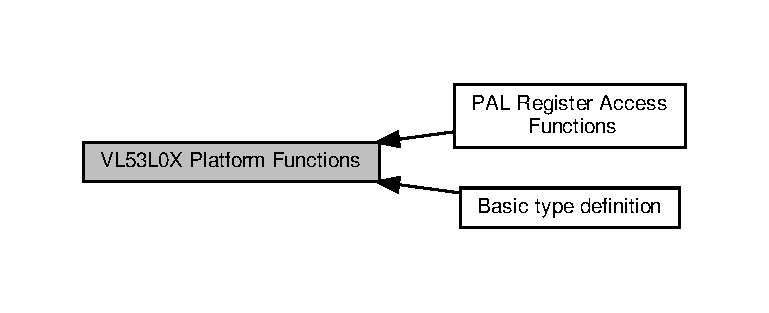
\includegraphics[width=350pt]{group__VL53L0X__platform__group}
\end{center}
\end{figure}
\subsection*{Modules}
\begin{DoxyCompactItemize}
\item 
\hyperlink{group__VL53L0X__registerAccess__group}{P\+A\+L Register Access Functions}
\begin{DoxyCompactList}\small\item\em P\+AL Register Access Functions. \end{DoxyCompactList}\item 
\hyperlink{group__porting__type}{Basic type definition}
\begin{DoxyCompactList}\small\item\em file \hyperlink{vl53l0x__types_8h}{vl53l0x\+\_\+types.\+h} files hold basic type definition that may requires porting \end{DoxyCompactList}\end{DoxyCompactItemize}
\subsection*{Classes}
\begin{DoxyCompactItemize}
\item 
struct \hyperlink{structVL53L0X__Dev__t}{V\+L53\+L0\+X\+\_\+\+Dev\+\_\+t}
\begin{DoxyCompactList}\small\item\em Generic P\+AL device type that does link between A\+PI and platform abstraction layer. \end{DoxyCompactList}\end{DoxyCompactItemize}
\subsection*{Macros}
\begin{DoxyCompactItemize}
\item 
\#define \hyperlink{group__VL53L0X__platform__group_ga21f3ef1fbe84f5cf77d989c95f21ad0a}{P\+A\+L\+Dev\+Data\+Get}(Dev,  field)~(Dev-\/$>$Data.\+field)
\begin{DoxyCompactList}\small\item\em Get ST private structure {\itshape \hyperlink{structVL53L0X__DevData__t}{V\+L53\+L0\+X\+\_\+\+Dev\+Data\+\_\+t}} data access. \end{DoxyCompactList}\item 
\#define \hyperlink{group__VL53L0X__platform__group_ga7d67a50d6fbce3ffdb71b4b3f7cbdf39}{P\+A\+L\+Dev\+Data\+Set}(Dev,  field,  data)~(Dev-\/$>$Data.\+field)=(data)
\begin{DoxyCompactList}\small\item\em Set ST private structure {\itshape \hyperlink{structVL53L0X__DevData__t}{V\+L53\+L0\+X\+\_\+\+Dev\+Data\+\_\+t}} data field. \end{DoxyCompactList}\end{DoxyCompactItemize}
\subsection*{Typedefs}
\begin{DoxyCompactItemize}
\item 
\mbox{\Hypertarget{group__VL53L0X__platform__group_ga2d6405308b1dd524b462f1b8fb97d167}\label{group__VL53L0X__platform__group_ga2d6405308b1dd524b462f1b8fb97d167}} 
typedef \hyperlink{structVL53L0X__Dev__t}{V\+L53\+L0\+X\+\_\+\+Dev\+\_\+t} $\ast$ \hyperlink{group__VL53L0X__platform__group_ga2d6405308b1dd524b462f1b8fb97d167}{V\+L53\+L0\+X\+\_\+\+D\+EV}
\begin{DoxyCompactList}\small\item\em Declare the device Handle as a pointer of the structure {\itshape \hyperlink{structVL53L0X__Dev__t}{V\+L53\+L0\+X\+\_\+\+Dev\+\_\+t}}. \end{DoxyCompactList}\end{DoxyCompactItemize}
\subsection*{Functions}
\begin{DoxyCompactItemize}
\item 
V\+L53\+L0\+X\+\_\+\+Error \hyperlink{group__VL53L0X__platform__group_ga08518599bfc34a2c943dcd5fa14072de}{V\+L53\+L0\+X\+\_\+\+Polling\+Delay} (\hyperlink{group__VL53L0X__platform__group_ga2d6405308b1dd524b462f1b8fb97d167}{V\+L53\+L0\+X\+\_\+\+D\+EV} Dev)
\begin{DoxyCompactList}\small\item\em execute delay in all polling A\+PI call \end{DoxyCompactList}\end{DoxyCompactItemize}


\subsection{Detailed Description}
V\+L53\+L0X Platform Functions. 



\subsection{Macro Definition Documentation}
\mbox{\Hypertarget{group__VL53L0X__platform__group_ga21f3ef1fbe84f5cf77d989c95f21ad0a}\label{group__VL53L0X__platform__group_ga21f3ef1fbe84f5cf77d989c95f21ad0a}} 
\index{V\+L53\+L0\+X Platform Functions@{V\+L53\+L0\+X Platform Functions}!P\+A\+L\+Dev\+Data\+Get@{P\+A\+L\+Dev\+Data\+Get}}
\index{P\+A\+L\+Dev\+Data\+Get@{P\+A\+L\+Dev\+Data\+Get}!V\+L53\+L0\+X Platform Functions@{V\+L53\+L0\+X Platform Functions}}
\subsubsection{\texorpdfstring{P\+A\+L\+Dev\+Data\+Get}{PALDevDataGet}}
{\footnotesize\ttfamily \#define P\+A\+L\+Dev\+Data\+Get(\begin{DoxyParamCaption}\item[{}]{Dev,  }\item[{}]{field }\end{DoxyParamCaption})~(Dev-\/$>$Data.\+field)}



Get ST private structure {\itshape \hyperlink{structVL53L0X__DevData__t}{V\+L53\+L0\+X\+\_\+\+Dev\+Data\+\_\+t}} data access. 


\begin{DoxyParams}{Parameters}
{\em Dev} & Device Handle \\
\hline
{\em field} & ST structure field name It maybe used and as real data \char`\"{}ref\char`\"{} not just as \char`\"{}get\char`\"{} for sub-\/structure item like P\+A\+L\+Dev\+Data\+Get(Filter\+Data.\+field)\mbox{[}i\mbox{]} or P\+A\+L\+Dev\+Data\+Get(Filter\+Data.\+Measurement\+Index)++ \\
\hline
\end{DoxyParams}
\mbox{\Hypertarget{group__VL53L0X__platform__group_ga7d67a50d6fbce3ffdb71b4b3f7cbdf39}\label{group__VL53L0X__platform__group_ga7d67a50d6fbce3ffdb71b4b3f7cbdf39}} 
\index{V\+L53\+L0\+X Platform Functions@{V\+L53\+L0\+X Platform Functions}!P\+A\+L\+Dev\+Data\+Set@{P\+A\+L\+Dev\+Data\+Set}}
\index{P\+A\+L\+Dev\+Data\+Set@{P\+A\+L\+Dev\+Data\+Set}!V\+L53\+L0\+X Platform Functions@{V\+L53\+L0\+X Platform Functions}}
\subsubsection{\texorpdfstring{P\+A\+L\+Dev\+Data\+Set}{PALDevDataSet}}
{\footnotesize\ttfamily \#define P\+A\+L\+Dev\+Data\+Set(\begin{DoxyParamCaption}\item[{}]{Dev,  }\item[{}]{field,  }\item[{}]{data }\end{DoxyParamCaption})~(Dev-\/$>$Data.\+field)=(data)}



Set ST private structure {\itshape \hyperlink{structVL53L0X__DevData__t}{V\+L53\+L0\+X\+\_\+\+Dev\+Data\+\_\+t}} data field. 


\begin{DoxyParams}{Parameters}
{\em Dev} & Device Handle \\
\hline
{\em field} & ST structure field name \\
\hline
{\em data} & Data to be set \\
\hline
\end{DoxyParams}


\subsection{Function Documentation}
\mbox{\Hypertarget{group__VL53L0X__platform__group_ga08518599bfc34a2c943dcd5fa14072de}\label{group__VL53L0X__platform__group_ga08518599bfc34a2c943dcd5fa14072de}} 
\index{V\+L53\+L0\+X Platform Functions@{V\+L53\+L0\+X Platform Functions}!V\+L53\+L0\+X\+\_\+\+Polling\+Delay@{V\+L53\+L0\+X\+\_\+\+Polling\+Delay}}
\index{V\+L53\+L0\+X\+\_\+\+Polling\+Delay@{V\+L53\+L0\+X\+\_\+\+Polling\+Delay}!V\+L53\+L0\+X Platform Functions@{V\+L53\+L0\+X Platform Functions}}
\subsubsection{\texorpdfstring{V\+L53\+L0\+X\+\_\+\+Polling\+Delay()}{VL53L0X\_PollingDelay()}}
{\footnotesize\ttfamily V\+L53\+L0\+X\+\_\+\+Error V\+L53\+L0\+X\+\_\+\+Polling\+Delay (\begin{DoxyParamCaption}\item[{\hyperlink{group__VL53L0X__platform__group_ga2d6405308b1dd524b462f1b8fb97d167}{V\+L53\+L0\+X\+\_\+\+D\+EV}}]{Dev }\end{DoxyParamCaption})}



execute delay in all polling A\+PI call 

A typical multi-\/thread or R\+T\+Os implementation is to sleep the task for some 5ms (with 100\+Hz max rate faster polling is not needed) if nothing specific is need you can define it as an empty/void macro 
\begin{DoxyCode}
\textcolor{preprocessor}{#define VL53L0X\_PollingDelay(...) (void)0}
\end{DoxyCode}
 
\begin{DoxyParams}{Parameters}
{\em Dev} & Device Handle \\
\hline
\end{DoxyParams}
\begin{DoxyReturn}{Returns}
V\+L53\+L0\+X\+\_\+\+E\+R\+R\+O\+R\+\_\+\+N\+O\+NE Success 

\char`\"{}\+Other error code\char`\"{} See \+::\+V\+L53\+L0\+X\+\_\+\+Error 
\end{DoxyReturn}

\hypertarget{group__VL53L0X__registerAccess__group}{}\section{P\+AL Register Access Functions}
\label{group__VL53L0X__registerAccess__group}\index{P\+A\+L Register Access Functions@{P\+A\+L Register Access Functions}}


P\+AL Register Access Functions.  


Collaboration diagram for P\+AL Register Access Functions\+:\nopagebreak
\begin{figure}[H]
\begin{center}
\leavevmode
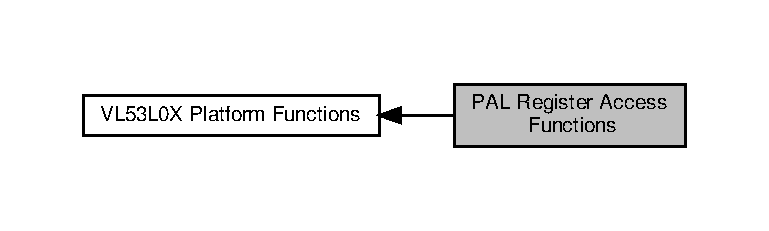
\includegraphics[width=350pt]{group__VL53L0X__registerAccess__group}
\end{center}
\end{figure}
\subsection*{Functions}
\begin{DoxyCompactItemize}
\item 
V\+L53\+L0\+X\+\_\+\+Error \hyperlink{group__VL53L0X__registerAccess__group_gadec2e01eacfb71e35303673dba4c525a}{V\+L53\+L0\+X\+\_\+\+Lock\+Sequence\+Access} (\hyperlink{group__VL53L0X__platform__group_ga2d6405308b1dd524b462f1b8fb97d167}{V\+L53\+L0\+X\+\_\+\+D\+EV} Dev)
\item 
V\+L53\+L0\+X\+\_\+\+Error \hyperlink{group__VL53L0X__registerAccess__group_gaa842ffc920a56baf1e790b98f52c2973}{V\+L53\+L0\+X\+\_\+\+Unlock\+Sequence\+Access} (\hyperlink{group__VL53L0X__platform__group_ga2d6405308b1dd524b462f1b8fb97d167}{V\+L53\+L0\+X\+\_\+\+D\+EV} Dev)
\item 
V\+L53\+L0\+X\+\_\+\+Error \hyperlink{group__VL53L0X__registerAccess__group_ga1bd43902504d62efa30bb7d1334becb7}{V\+L53\+L0\+X\+\_\+\+Write\+Multi} (\hyperlink{group__VL53L0X__platform__group_ga2d6405308b1dd524b462f1b8fb97d167}{V\+L53\+L0\+X\+\_\+\+D\+EV} Dev, \hyperlink{vl53l0x__types_8h_aba7bc1797add20fe3efdf37ced1182c5}{uint8\+\_\+t} index, \hyperlink{vl53l0x__types_8h_aba7bc1797add20fe3efdf37ced1182c5}{uint8\+\_\+t} $\ast$pdata, \hyperlink{vl53l0x__types_8h_a435d1572bf3f880d55459d9805097f62}{uint32\+\_\+t} count)
\item 
V\+L53\+L0\+X\+\_\+\+Error \hyperlink{group__VL53L0X__registerAccess__group_ga7ada799fc93691cea5dde0cae5e3ab58}{V\+L53\+L0\+X\+\_\+\+Read\+Multi} (\hyperlink{group__VL53L0X__platform__group_ga2d6405308b1dd524b462f1b8fb97d167}{V\+L53\+L0\+X\+\_\+\+D\+EV} Dev, \hyperlink{vl53l0x__types_8h_aba7bc1797add20fe3efdf37ced1182c5}{uint8\+\_\+t} index, \hyperlink{vl53l0x__types_8h_aba7bc1797add20fe3efdf37ced1182c5}{uint8\+\_\+t} $\ast$pdata, \hyperlink{vl53l0x__types_8h_a435d1572bf3f880d55459d9805097f62}{uint32\+\_\+t} count)
\item 
V\+L53\+L0\+X\+\_\+\+Error \hyperlink{group__VL53L0X__registerAccess__group_ga17c6507a39dac954c01ef78a6bd27ca1}{V\+L53\+L0\+X\+\_\+\+Wr\+Byte} (\hyperlink{group__VL53L0X__platform__group_ga2d6405308b1dd524b462f1b8fb97d167}{V\+L53\+L0\+X\+\_\+\+D\+EV} Dev, \hyperlink{vl53l0x__types_8h_aba7bc1797add20fe3efdf37ced1182c5}{uint8\+\_\+t} index, \hyperlink{vl53l0x__types_8h_aba7bc1797add20fe3efdf37ced1182c5}{uint8\+\_\+t} data)
\item 
V\+L53\+L0\+X\+\_\+\+Error \hyperlink{group__VL53L0X__registerAccess__group_gadc1bb94017f349842e439db5a3d0fea8}{V\+L53\+L0\+X\+\_\+\+Wr\+Word} (\hyperlink{group__VL53L0X__platform__group_ga2d6405308b1dd524b462f1b8fb97d167}{V\+L53\+L0\+X\+\_\+\+D\+EV} Dev, \hyperlink{vl53l0x__types_8h_aba7bc1797add20fe3efdf37ced1182c5}{uint8\+\_\+t} index, \hyperlink{vl53l0x__types_8h_a273cf69d639a59973b6019625df33e30}{uint16\+\_\+t} data)
\item 
V\+L53\+L0\+X\+\_\+\+Error \hyperlink{group__VL53L0X__registerAccess__group_ga0a117141cf0e6b0a4b97935a367482d5}{V\+L53\+L0\+X\+\_\+\+Wr\+D\+Word} (\hyperlink{group__VL53L0X__platform__group_ga2d6405308b1dd524b462f1b8fb97d167}{V\+L53\+L0\+X\+\_\+\+D\+EV} Dev, \hyperlink{vl53l0x__types_8h_aba7bc1797add20fe3efdf37ced1182c5}{uint8\+\_\+t} index, \hyperlink{vl53l0x__types_8h_a435d1572bf3f880d55459d9805097f62}{uint32\+\_\+t} data)
\item 
V\+L53\+L0\+X\+\_\+\+Error \hyperlink{group__VL53L0X__registerAccess__group_gaab280eabdced8065bc4fb99e221e12f9}{V\+L53\+L0\+X\+\_\+\+Rd\+Byte} (\hyperlink{group__VL53L0X__platform__group_ga2d6405308b1dd524b462f1b8fb97d167}{V\+L53\+L0\+X\+\_\+\+D\+EV} Dev, \hyperlink{vl53l0x__types_8h_aba7bc1797add20fe3efdf37ced1182c5}{uint8\+\_\+t} index, \hyperlink{vl53l0x__types_8h_aba7bc1797add20fe3efdf37ced1182c5}{uint8\+\_\+t} $\ast$data)
\item 
V\+L53\+L0\+X\+\_\+\+Error \hyperlink{group__VL53L0X__registerAccess__group_gabff46b6c5c984c2b6b11783f1c640558}{V\+L53\+L0\+X\+\_\+\+Rd\+Word} (\hyperlink{group__VL53L0X__platform__group_ga2d6405308b1dd524b462f1b8fb97d167}{V\+L53\+L0\+X\+\_\+\+D\+EV} Dev, \hyperlink{vl53l0x__types_8h_aba7bc1797add20fe3efdf37ced1182c5}{uint8\+\_\+t} index, \hyperlink{vl53l0x__types_8h_a273cf69d639a59973b6019625df33e30}{uint16\+\_\+t} $\ast$data)
\item 
V\+L53\+L0\+X\+\_\+\+Error \hyperlink{group__VL53L0X__registerAccess__group_ga18d1e6fe40708046d611d581f20d735b}{V\+L53\+L0\+X\+\_\+\+Rd\+D\+Word} (\hyperlink{group__VL53L0X__platform__group_ga2d6405308b1dd524b462f1b8fb97d167}{V\+L53\+L0\+X\+\_\+\+D\+EV} Dev, \hyperlink{vl53l0x__types_8h_aba7bc1797add20fe3efdf37ced1182c5}{uint8\+\_\+t} index, \hyperlink{vl53l0x__types_8h_a435d1572bf3f880d55459d9805097f62}{uint32\+\_\+t} $\ast$data)
\item 
V\+L53\+L0\+X\+\_\+\+Error \hyperlink{group__VL53L0X__registerAccess__group_gaf8c163567d7906d16cad171957bf4198}{V\+L53\+L0\+X\+\_\+\+Update\+Byte} (\hyperlink{group__VL53L0X__platform__group_ga2d6405308b1dd524b462f1b8fb97d167}{V\+L53\+L0\+X\+\_\+\+D\+EV} Dev, \hyperlink{vl53l0x__types_8h_aba7bc1797add20fe3efdf37ced1182c5}{uint8\+\_\+t} index, \hyperlink{vl53l0x__types_8h_aba7bc1797add20fe3efdf37ced1182c5}{uint8\+\_\+t} And\+Data, \hyperlink{vl53l0x__types_8h_aba7bc1797add20fe3efdf37ced1182c5}{uint8\+\_\+t} Or\+Data)
\end{DoxyCompactItemize}


\subsection{Detailed Description}
P\+AL Register Access Functions. 



\subsection{Function Documentation}
\mbox{\Hypertarget{group__VL53L0X__registerAccess__group_gadec2e01eacfb71e35303673dba4c525a}\label{group__VL53L0X__registerAccess__group_gadec2e01eacfb71e35303673dba4c525a}} 
\index{P\+A\+L Register Access Functions@{P\+A\+L Register Access Functions}!V\+L53\+L0\+X\+\_\+\+Lock\+Sequence\+Access@{V\+L53\+L0\+X\+\_\+\+Lock\+Sequence\+Access}}
\index{V\+L53\+L0\+X\+\_\+\+Lock\+Sequence\+Access@{V\+L53\+L0\+X\+\_\+\+Lock\+Sequence\+Access}!P\+A\+L Register Access Functions@{P\+A\+L Register Access Functions}}
\subsubsection{\texorpdfstring{V\+L53\+L0\+X\+\_\+\+Lock\+Sequence\+Access()}{VL53L0X\_LockSequenceAccess()}}
{\footnotesize\ttfamily V\+L53\+L0\+X\+\_\+\+Error V\+L53\+L0\+X\+\_\+\+Lock\+Sequence\+Access (\begin{DoxyParamCaption}\item[{\hyperlink{group__VL53L0X__platform__group_ga2d6405308b1dd524b462f1b8fb97d167}{V\+L53\+L0\+X\+\_\+\+D\+EV}}]{Dev }\end{DoxyParamCaption})}

Lock comms interface to serialize all commands to a shared I2C interface for a specific device 
\begin{DoxyParams}{Parameters}
{\em Dev} & Device Handle \\
\hline
\end{DoxyParams}
\begin{DoxyReturn}{Returns}
V\+L53\+L0\+X\+\_\+\+E\+R\+R\+O\+R\+\_\+\+N\+O\+NE Success 

\char`\"{}\+Other error code\char`\"{} See \+::\+V\+L53\+L0\+X\+\_\+\+Error 
\end{DoxyReturn}
\mbox{\Hypertarget{group__VL53L0X__registerAccess__group_gaab280eabdced8065bc4fb99e221e12f9}\label{group__VL53L0X__registerAccess__group_gaab280eabdced8065bc4fb99e221e12f9}} 
\index{P\+A\+L Register Access Functions@{P\+A\+L Register Access Functions}!V\+L53\+L0\+X\+\_\+\+Rd\+Byte@{V\+L53\+L0\+X\+\_\+\+Rd\+Byte}}
\index{V\+L53\+L0\+X\+\_\+\+Rd\+Byte@{V\+L53\+L0\+X\+\_\+\+Rd\+Byte}!P\+A\+L Register Access Functions@{P\+A\+L Register Access Functions}}
\subsubsection{\texorpdfstring{V\+L53\+L0\+X\+\_\+\+Rd\+Byte()}{VL53L0X\_RdByte()}}
{\footnotesize\ttfamily V\+L53\+L0\+X\+\_\+\+Error V\+L53\+L0\+X\+\_\+\+Rd\+Byte (\begin{DoxyParamCaption}\item[{\hyperlink{group__VL53L0X__platform__group_ga2d6405308b1dd524b462f1b8fb97d167}{V\+L53\+L0\+X\+\_\+\+D\+EV}}]{Dev,  }\item[{\hyperlink{vl53l0x__types_8h_aba7bc1797add20fe3efdf37ced1182c5}{uint8\+\_\+t}}]{index,  }\item[{\hyperlink{vl53l0x__types_8h_aba7bc1797add20fe3efdf37ced1182c5}{uint8\+\_\+t} $\ast$}]{data }\end{DoxyParamCaption})}

Read single byte register 
\begin{DoxyParams}{Parameters}
{\em Dev} & Device Handle \\
\hline
{\em index} & \hyperlink{structThe}{The} register index \\
\hline
{\em data} & pointer to 8 bit data \\
\hline
\end{DoxyParams}
\begin{DoxyReturn}{Returns}
V\+L53\+L0\+X\+\_\+\+E\+R\+R\+O\+R\+\_\+\+N\+O\+NE Success 

\char`\"{}\+Other error code\char`\"{} See \+::\+V\+L53\+L0\+X\+\_\+\+Error 
\end{DoxyReturn}
\mbox{\Hypertarget{group__VL53L0X__registerAccess__group_ga18d1e6fe40708046d611d581f20d735b}\label{group__VL53L0X__registerAccess__group_ga18d1e6fe40708046d611d581f20d735b}} 
\index{P\+A\+L Register Access Functions@{P\+A\+L Register Access Functions}!V\+L53\+L0\+X\+\_\+\+Rd\+D\+Word@{V\+L53\+L0\+X\+\_\+\+Rd\+D\+Word}}
\index{V\+L53\+L0\+X\+\_\+\+Rd\+D\+Word@{V\+L53\+L0\+X\+\_\+\+Rd\+D\+Word}!P\+A\+L Register Access Functions@{P\+A\+L Register Access Functions}}
\subsubsection{\texorpdfstring{V\+L53\+L0\+X\+\_\+\+Rd\+D\+Word()}{VL53L0X\_RdDWord()}}
{\footnotesize\ttfamily V\+L53\+L0\+X\+\_\+\+Error V\+L53\+L0\+X\+\_\+\+Rd\+D\+Word (\begin{DoxyParamCaption}\item[{\hyperlink{group__VL53L0X__platform__group_ga2d6405308b1dd524b462f1b8fb97d167}{V\+L53\+L0\+X\+\_\+\+D\+EV}}]{Dev,  }\item[{\hyperlink{vl53l0x__types_8h_aba7bc1797add20fe3efdf37ced1182c5}{uint8\+\_\+t}}]{index,  }\item[{\hyperlink{vl53l0x__types_8h_a435d1572bf3f880d55459d9805097f62}{uint32\+\_\+t} $\ast$}]{data }\end{DoxyParamCaption})}

Read dword (4byte) register 
\begin{DoxyParams}{Parameters}
{\em Dev} & Device Handle \\
\hline
{\em index} & \hyperlink{structThe}{The} register index \\
\hline
{\em data} & pointer to 32 bit data \\
\hline
\end{DoxyParams}
\begin{DoxyReturn}{Returns}
V\+L53\+L0\+X\+\_\+\+E\+R\+R\+O\+R\+\_\+\+N\+O\+NE Success 

\char`\"{}\+Other error code\char`\"{} See \+::\+V\+L53\+L0\+X\+\_\+\+Error 
\end{DoxyReturn}
\mbox{\Hypertarget{group__VL53L0X__registerAccess__group_gabff46b6c5c984c2b6b11783f1c640558}\label{group__VL53L0X__registerAccess__group_gabff46b6c5c984c2b6b11783f1c640558}} 
\index{P\+A\+L Register Access Functions@{P\+A\+L Register Access Functions}!V\+L53\+L0\+X\+\_\+\+Rd\+Word@{V\+L53\+L0\+X\+\_\+\+Rd\+Word}}
\index{V\+L53\+L0\+X\+\_\+\+Rd\+Word@{V\+L53\+L0\+X\+\_\+\+Rd\+Word}!P\+A\+L Register Access Functions@{P\+A\+L Register Access Functions}}
\subsubsection{\texorpdfstring{V\+L53\+L0\+X\+\_\+\+Rd\+Word()}{VL53L0X\_RdWord()}}
{\footnotesize\ttfamily V\+L53\+L0\+X\+\_\+\+Error V\+L53\+L0\+X\+\_\+\+Rd\+Word (\begin{DoxyParamCaption}\item[{\hyperlink{group__VL53L0X__platform__group_ga2d6405308b1dd524b462f1b8fb97d167}{V\+L53\+L0\+X\+\_\+\+D\+EV}}]{Dev,  }\item[{\hyperlink{vl53l0x__types_8h_aba7bc1797add20fe3efdf37ced1182c5}{uint8\+\_\+t}}]{index,  }\item[{\hyperlink{vl53l0x__types_8h_a273cf69d639a59973b6019625df33e30}{uint16\+\_\+t} $\ast$}]{data }\end{DoxyParamCaption})}

Read word (2byte) register 
\begin{DoxyParams}{Parameters}
{\em Dev} & Device Handle \\
\hline
{\em index} & \hyperlink{structThe}{The} register index \\
\hline
{\em data} & pointer to 16 bit data \\
\hline
\end{DoxyParams}
\begin{DoxyReturn}{Returns}
V\+L53\+L0\+X\+\_\+\+E\+R\+R\+O\+R\+\_\+\+N\+O\+NE Success 

\char`\"{}\+Other error code\char`\"{} See \+::\+V\+L53\+L0\+X\+\_\+\+Error 
\end{DoxyReturn}
\mbox{\Hypertarget{group__VL53L0X__registerAccess__group_ga7ada799fc93691cea5dde0cae5e3ab58}\label{group__VL53L0X__registerAccess__group_ga7ada799fc93691cea5dde0cae5e3ab58}} 
\index{P\+A\+L Register Access Functions@{P\+A\+L Register Access Functions}!V\+L53\+L0\+X\+\_\+\+Read\+Multi@{V\+L53\+L0\+X\+\_\+\+Read\+Multi}}
\index{V\+L53\+L0\+X\+\_\+\+Read\+Multi@{V\+L53\+L0\+X\+\_\+\+Read\+Multi}!P\+A\+L Register Access Functions@{P\+A\+L Register Access Functions}}
\subsubsection{\texorpdfstring{V\+L53\+L0\+X\+\_\+\+Read\+Multi()}{VL53L0X\_ReadMulti()}}
{\footnotesize\ttfamily V\+L53\+L0\+X\+\_\+\+Error V\+L53\+L0\+X\+\_\+\+Read\+Multi (\begin{DoxyParamCaption}\item[{\hyperlink{group__VL53L0X__platform__group_ga2d6405308b1dd524b462f1b8fb97d167}{V\+L53\+L0\+X\+\_\+\+D\+EV}}]{Dev,  }\item[{\hyperlink{vl53l0x__types_8h_aba7bc1797add20fe3efdf37ced1182c5}{uint8\+\_\+t}}]{index,  }\item[{\hyperlink{vl53l0x__types_8h_aba7bc1797add20fe3efdf37ced1182c5}{uint8\+\_\+t} $\ast$}]{pdata,  }\item[{\hyperlink{vl53l0x__types_8h_a435d1572bf3f880d55459d9805097f62}{uint32\+\_\+t}}]{count }\end{DoxyParamCaption})}

Reads the requested number of bytes from the device 
\begin{DoxyParams}{Parameters}
{\em Dev} & Device Handle \\
\hline
{\em index} & \hyperlink{structThe}{The} register index \\
\hline
{\em pdata} & Pointer to the uint8\+\_\+t buffer to store read data \\
\hline
{\em count} & Number of uint8\+\_\+t\textquotesingle{}s to read \\
\hline
\end{DoxyParams}
\begin{DoxyReturn}{Returns}
V\+L53\+L0\+X\+\_\+\+E\+R\+R\+O\+R\+\_\+\+N\+O\+NE Success 

\char`\"{}\+Other error code\char`\"{} See \+::\+V\+L53\+L0\+X\+\_\+\+Error 
\end{DoxyReturn}
\mbox{\Hypertarget{group__VL53L0X__registerAccess__group_gaa842ffc920a56baf1e790b98f52c2973}\label{group__VL53L0X__registerAccess__group_gaa842ffc920a56baf1e790b98f52c2973}} 
\index{P\+A\+L Register Access Functions@{P\+A\+L Register Access Functions}!V\+L53\+L0\+X\+\_\+\+Unlock\+Sequence\+Access@{V\+L53\+L0\+X\+\_\+\+Unlock\+Sequence\+Access}}
\index{V\+L53\+L0\+X\+\_\+\+Unlock\+Sequence\+Access@{V\+L53\+L0\+X\+\_\+\+Unlock\+Sequence\+Access}!P\+A\+L Register Access Functions@{P\+A\+L Register Access Functions}}
\subsubsection{\texorpdfstring{V\+L53\+L0\+X\+\_\+\+Unlock\+Sequence\+Access()}{VL53L0X\_UnlockSequenceAccess()}}
{\footnotesize\ttfamily V\+L53\+L0\+X\+\_\+\+Error V\+L53\+L0\+X\+\_\+\+Unlock\+Sequence\+Access (\begin{DoxyParamCaption}\item[{\hyperlink{group__VL53L0X__platform__group_ga2d6405308b1dd524b462f1b8fb97d167}{V\+L53\+L0\+X\+\_\+\+D\+EV}}]{Dev }\end{DoxyParamCaption})}

Unlock comms interface to serialize all commands to a shared I2C interface for a specific device 
\begin{DoxyParams}{Parameters}
{\em Dev} & Device Handle \\
\hline
\end{DoxyParams}
\begin{DoxyReturn}{Returns}
V\+L53\+L0\+X\+\_\+\+E\+R\+R\+O\+R\+\_\+\+N\+O\+NE Success 

\char`\"{}\+Other error code\char`\"{} See \+::\+V\+L53\+L0\+X\+\_\+\+Error 
\end{DoxyReturn}
\mbox{\Hypertarget{group__VL53L0X__registerAccess__group_gaf8c163567d7906d16cad171957bf4198}\label{group__VL53L0X__registerAccess__group_gaf8c163567d7906d16cad171957bf4198}} 
\index{P\+A\+L Register Access Functions@{P\+A\+L Register Access Functions}!V\+L53\+L0\+X\+\_\+\+Update\+Byte@{V\+L53\+L0\+X\+\_\+\+Update\+Byte}}
\index{V\+L53\+L0\+X\+\_\+\+Update\+Byte@{V\+L53\+L0\+X\+\_\+\+Update\+Byte}!P\+A\+L Register Access Functions@{P\+A\+L Register Access Functions}}
\subsubsection{\texorpdfstring{V\+L53\+L0\+X\+\_\+\+Update\+Byte()}{VL53L0X\_UpdateByte()}}
{\footnotesize\ttfamily V\+L53\+L0\+X\+\_\+\+Error V\+L53\+L0\+X\+\_\+\+Update\+Byte (\begin{DoxyParamCaption}\item[{\hyperlink{group__VL53L0X__platform__group_ga2d6405308b1dd524b462f1b8fb97d167}{V\+L53\+L0\+X\+\_\+\+D\+EV}}]{Dev,  }\item[{\hyperlink{vl53l0x__types_8h_aba7bc1797add20fe3efdf37ced1182c5}{uint8\+\_\+t}}]{index,  }\item[{\hyperlink{vl53l0x__types_8h_aba7bc1797add20fe3efdf37ced1182c5}{uint8\+\_\+t}}]{And\+Data,  }\item[{\hyperlink{vl53l0x__types_8h_aba7bc1797add20fe3efdf37ced1182c5}{uint8\+\_\+t}}]{Or\+Data }\end{DoxyParamCaption})}

Threat safe Update (read/modify/write) single byte register

Final\+\_\+reg = (Initial\+\_\+reg \& and\+\_\+data) $\vert$or\+\_\+data


\begin{DoxyParams}{Parameters}
{\em Dev} & Device Handle \\
\hline
{\em index} & \hyperlink{structThe}{The} register index \\
\hline
{\em And\+Data} & 8 bit and data \\
\hline
{\em Or\+Data} & 8 bit or data \\
\hline
\end{DoxyParams}
\begin{DoxyReturn}{Returns}
V\+L53\+L0\+X\+\_\+\+E\+R\+R\+O\+R\+\_\+\+N\+O\+NE Success 

\char`\"{}\+Other error code\char`\"{} See \+::\+V\+L53\+L0\+X\+\_\+\+Error 
\end{DoxyReturn}
\mbox{\Hypertarget{group__VL53L0X__registerAccess__group_ga17c6507a39dac954c01ef78a6bd27ca1}\label{group__VL53L0X__registerAccess__group_ga17c6507a39dac954c01ef78a6bd27ca1}} 
\index{P\+A\+L Register Access Functions@{P\+A\+L Register Access Functions}!V\+L53\+L0\+X\+\_\+\+Wr\+Byte@{V\+L53\+L0\+X\+\_\+\+Wr\+Byte}}
\index{V\+L53\+L0\+X\+\_\+\+Wr\+Byte@{V\+L53\+L0\+X\+\_\+\+Wr\+Byte}!P\+A\+L Register Access Functions@{P\+A\+L Register Access Functions}}
\subsubsection{\texorpdfstring{V\+L53\+L0\+X\+\_\+\+Wr\+Byte()}{VL53L0X\_WrByte()}}
{\footnotesize\ttfamily V\+L53\+L0\+X\+\_\+\+Error V\+L53\+L0\+X\+\_\+\+Wr\+Byte (\begin{DoxyParamCaption}\item[{\hyperlink{group__VL53L0X__platform__group_ga2d6405308b1dd524b462f1b8fb97d167}{V\+L53\+L0\+X\+\_\+\+D\+EV}}]{Dev,  }\item[{\hyperlink{vl53l0x__types_8h_aba7bc1797add20fe3efdf37ced1182c5}{uint8\+\_\+t}}]{index,  }\item[{\hyperlink{vl53l0x__types_8h_aba7bc1797add20fe3efdf37ced1182c5}{uint8\+\_\+t}}]{data }\end{DoxyParamCaption})}

Write single byte register 
\begin{DoxyParams}{Parameters}
{\em Dev} & Device Handle \\
\hline
{\em index} & \hyperlink{structThe}{The} register index \\
\hline
{\em data} & 8 bit register data \\
\hline
\end{DoxyParams}
\begin{DoxyReturn}{Returns}
V\+L53\+L0\+X\+\_\+\+E\+R\+R\+O\+R\+\_\+\+N\+O\+NE Success 

\char`\"{}\+Other error code\char`\"{} See \+::\+V\+L53\+L0\+X\+\_\+\+Error 
\end{DoxyReturn}
\mbox{\Hypertarget{group__VL53L0X__registerAccess__group_ga0a117141cf0e6b0a4b97935a367482d5}\label{group__VL53L0X__registerAccess__group_ga0a117141cf0e6b0a4b97935a367482d5}} 
\index{P\+A\+L Register Access Functions@{P\+A\+L Register Access Functions}!V\+L53\+L0\+X\+\_\+\+Wr\+D\+Word@{V\+L53\+L0\+X\+\_\+\+Wr\+D\+Word}}
\index{V\+L53\+L0\+X\+\_\+\+Wr\+D\+Word@{V\+L53\+L0\+X\+\_\+\+Wr\+D\+Word}!P\+A\+L Register Access Functions@{P\+A\+L Register Access Functions}}
\subsubsection{\texorpdfstring{V\+L53\+L0\+X\+\_\+\+Wr\+D\+Word()}{VL53L0X\_WrDWord()}}
{\footnotesize\ttfamily V\+L53\+L0\+X\+\_\+\+Error V\+L53\+L0\+X\+\_\+\+Wr\+D\+Word (\begin{DoxyParamCaption}\item[{\hyperlink{group__VL53L0X__platform__group_ga2d6405308b1dd524b462f1b8fb97d167}{V\+L53\+L0\+X\+\_\+\+D\+EV}}]{Dev,  }\item[{\hyperlink{vl53l0x__types_8h_aba7bc1797add20fe3efdf37ced1182c5}{uint8\+\_\+t}}]{index,  }\item[{\hyperlink{vl53l0x__types_8h_a435d1572bf3f880d55459d9805097f62}{uint32\+\_\+t}}]{data }\end{DoxyParamCaption})}

Write double word (4 byte) register 
\begin{DoxyParams}{Parameters}
{\em Dev} & Device Handle \\
\hline
{\em index} & \hyperlink{structThe}{The} register index \\
\hline
{\em data} & 32 bit register data \\
\hline
\end{DoxyParams}
\begin{DoxyReturn}{Returns}
V\+L53\+L0\+X\+\_\+\+E\+R\+R\+O\+R\+\_\+\+N\+O\+NE Success 

\char`\"{}\+Other error code\char`\"{} See \+::\+V\+L53\+L0\+X\+\_\+\+Error 
\end{DoxyReturn}
\mbox{\Hypertarget{group__VL53L0X__registerAccess__group_ga1bd43902504d62efa30bb7d1334becb7}\label{group__VL53L0X__registerAccess__group_ga1bd43902504d62efa30bb7d1334becb7}} 
\index{P\+A\+L Register Access Functions@{P\+A\+L Register Access Functions}!V\+L53\+L0\+X\+\_\+\+Write\+Multi@{V\+L53\+L0\+X\+\_\+\+Write\+Multi}}
\index{V\+L53\+L0\+X\+\_\+\+Write\+Multi@{V\+L53\+L0\+X\+\_\+\+Write\+Multi}!P\+A\+L Register Access Functions@{P\+A\+L Register Access Functions}}
\subsubsection{\texorpdfstring{V\+L53\+L0\+X\+\_\+\+Write\+Multi()}{VL53L0X\_WriteMulti()}}
{\footnotesize\ttfamily V\+L53\+L0\+X\+\_\+\+Error V\+L53\+L0\+X\+\_\+\+Write\+Multi (\begin{DoxyParamCaption}\item[{\hyperlink{group__VL53L0X__platform__group_ga2d6405308b1dd524b462f1b8fb97d167}{V\+L53\+L0\+X\+\_\+\+D\+EV}}]{Dev,  }\item[{\hyperlink{vl53l0x__types_8h_aba7bc1797add20fe3efdf37ced1182c5}{uint8\+\_\+t}}]{index,  }\item[{\hyperlink{vl53l0x__types_8h_aba7bc1797add20fe3efdf37ced1182c5}{uint8\+\_\+t} $\ast$}]{pdata,  }\item[{\hyperlink{vl53l0x__types_8h_a435d1572bf3f880d55459d9805097f62}{uint32\+\_\+t}}]{count }\end{DoxyParamCaption})}

Writes the supplied byte buffer to the device 
\begin{DoxyParams}{Parameters}
{\em Dev} & Device Handle \\
\hline
{\em index} & \hyperlink{structThe}{The} register index \\
\hline
{\em pdata} & Pointer to uint8\+\_\+t buffer containing the data to be written \\
\hline
{\em count} & Number of bytes in the supplied byte buffer \\
\hline
\end{DoxyParams}
\begin{DoxyReturn}{Returns}
V\+L53\+L0\+X\+\_\+\+E\+R\+R\+O\+R\+\_\+\+N\+O\+NE Success 

\char`\"{}\+Other error code\char`\"{} See \+::\+V\+L53\+L0\+X\+\_\+\+Error 
\end{DoxyReturn}
\mbox{\Hypertarget{group__VL53L0X__registerAccess__group_gadc1bb94017f349842e439db5a3d0fea8}\label{group__VL53L0X__registerAccess__group_gadc1bb94017f349842e439db5a3d0fea8}} 
\index{P\+A\+L Register Access Functions@{P\+A\+L Register Access Functions}!V\+L53\+L0\+X\+\_\+\+Wr\+Word@{V\+L53\+L0\+X\+\_\+\+Wr\+Word}}
\index{V\+L53\+L0\+X\+\_\+\+Wr\+Word@{V\+L53\+L0\+X\+\_\+\+Wr\+Word}!P\+A\+L Register Access Functions@{P\+A\+L Register Access Functions}}
\subsubsection{\texorpdfstring{V\+L53\+L0\+X\+\_\+\+Wr\+Word()}{VL53L0X\_WrWord()}}
{\footnotesize\ttfamily V\+L53\+L0\+X\+\_\+\+Error V\+L53\+L0\+X\+\_\+\+Wr\+Word (\begin{DoxyParamCaption}\item[{\hyperlink{group__VL53L0X__platform__group_ga2d6405308b1dd524b462f1b8fb97d167}{V\+L53\+L0\+X\+\_\+\+D\+EV}}]{Dev,  }\item[{\hyperlink{vl53l0x__types_8h_aba7bc1797add20fe3efdf37ced1182c5}{uint8\+\_\+t}}]{index,  }\item[{\hyperlink{vl53l0x__types_8h_a273cf69d639a59973b6019625df33e30}{uint16\+\_\+t}}]{data }\end{DoxyParamCaption})}

Write word register 
\begin{DoxyParams}{Parameters}
{\em Dev} & Device Handle \\
\hline
{\em index} & \hyperlink{structThe}{The} register index \\
\hline
{\em data} & 16 bit register data \\
\hline
\end{DoxyParams}
\begin{DoxyReturn}{Returns}
V\+L53\+L0\+X\+\_\+\+E\+R\+R\+O\+R\+\_\+\+N\+O\+NE Success 

\char`\"{}\+Other error code\char`\"{} See \+::\+V\+L53\+L0\+X\+\_\+\+Error 
\end{DoxyReturn}

\hypertarget{group__porting__type}{}\section{Basic type definition}
\label{group__porting__type}\index{Basic type definition@{Basic type definition}}


file \hyperlink{vl53l0x__types_8h}{vl53l0x\+\_\+types.\+h} files hold basic type definition that may requires porting  


Collaboration diagram for Basic type definition\+:\nopagebreak
\begin{figure}[H]
\begin{center}
\leavevmode
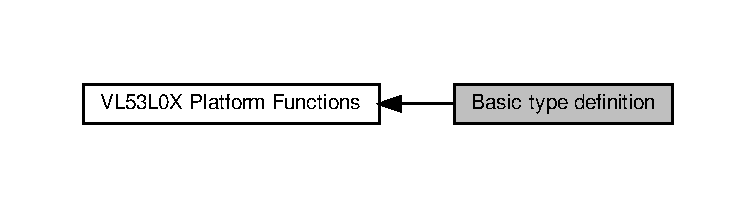
\includegraphics[width=350pt]{group__porting__type}
\end{center}
\end{figure}
file \hyperlink{vl53l0x__types_8h}{vl53l0x\+\_\+types.\+h} files hold basic type definition that may requires porting 

contains type that must be defined for the platform~\newline
when target platform and compiler provide stdint.\+h and stddef.\+h it is enough to include it.~\newline
If stdint.\+h is not available review and adapt all signed and unsigned 8/16/32 bits basic types. ~\newline
If stddef.\+h is not available review and adapt N\+U\+LL definition . 
\hypertarget{group__calc__sigma__estimate}{}\section{Calc\+\_\+sigma\+\_\+estimate}
\label{group__calc__sigma__estimate}\index{Calc\+\_\+sigma\+\_\+estimate@{Calc\+\_\+sigma\+\_\+estimate}}
\subsection*{Functions}
\begin{DoxyCompactItemize}
\item 
\mbox{\Hypertarget{group__calc__sigma__estimate_gac7b145a42321621d506540b81b33ceb6}\label{group__calc__sigma__estimate_gac7b145a42321621d506540b81b33ceb6}} 
V\+L53\+L0\+X\+\_\+\+Error {\bfseries V\+L53\+L0\+X\+\_\+get\+\_\+pal\+\_\+range\+\_\+status} (\hyperlink{group__VL53L0X__platform__group_ga2d6405308b1dd524b462f1b8fb97d167}{V\+L53\+L0\+X\+\_\+\+D\+EV} Dev, \hyperlink{vl53l0x__types_8h_aba7bc1797add20fe3efdf37ced1182c5}{uint8\+\_\+t} Device\+Range\+Status, \hyperlink{vl53l0x__types_8h_afb910790161809fc76e1a274a6349384}{Fix\+Point1616\+\_\+t} Signal\+Rate, \hyperlink{vl53l0x__types_8h_a273cf69d639a59973b6019625df33e30}{uint16\+\_\+t} Effective\+Spad\+Rtn\+Count, \hyperlink{structVL53L0X__RangingMeasurementData__t}{V\+L53\+L0\+X\+\_\+\+Ranging\+Measurement\+Data\+\_\+t} $\ast$p\+Ranging\+Measurement\+Data, \hyperlink{vl53l0x__types_8h_aba7bc1797add20fe3efdf37ced1182c5}{uint8\+\_\+t} $\ast$p\+Pal\+Range\+Status)
\end{DoxyCompactItemize}


\subsection{Detailed Description}
Estimates the range sigma
\chapter{Class Documentation}
\hypertarget{structA4988__Driver}{}\section{A4988\+\_\+\+Driver Struct Reference}
\label{structA4988__Driver}\index{A4988\+\_\+\+Driver@{A4988\+\_\+\+Driver}}
\subsection*{Public Attributes}
\begin{DoxyCompactItemize}
\item 
gpio\+\_\+num\+\_\+t \hyperlink{structA4988__Driver_ad70b2030eb7693eaa687f27af7889969}{sleep}
\item 
gpio\+\_\+num\+\_\+t \hyperlink{structA4988__Driver_a3f1250fca864ff2fa4b11a644cdcab17}{enable}
\item 
gpio\+\_\+num\+\_\+t \hyperlink{structA4988__Driver_a4209422243dd83633849726f74b40e7c}{step}
\item 
gpio\+\_\+num\+\_\+t \hyperlink{structA4988__Driver_a496834da227b845b4eaf969e726a177b}{rst}
\item 
gpio\+\_\+num\+\_\+t \hyperlink{structA4988__Driver_a52bcf5bee0f17eb8c8cfada6b74ce52f}{dir}
\item 
gpio\+\_\+num\+\_\+t \hyperlink{structA4988__Driver_a25111ec2990df3c0746cbd8850159d6b}{ms1}
\item 
gpio\+\_\+num\+\_\+t \hyperlink{structA4988__Driver_abb7be73306c0a811d8de796b75636fd9}{ms2}
\item 
gpio\+\_\+num\+\_\+t \hyperlink{structA4988__Driver_a2c218a9775018210e5683878894a3b7f}{ms3}
\item 
\hyperlink{vl53l0x__types_8h_a435d1572bf3f880d55459d9805097f62}{uint32\+\_\+t} \hyperlink{structA4988__Driver_ac99aedce09cf5509d686e81cb896fd6e}{step\+\_\+pulse\+\_\+len}
\item 
\hyperlink{vl53l0x__types_8h_a435d1572bf3f880d55459d9805097f62}{uint32\+\_\+t} \hyperlink{structA4988__Driver_a14b08b6fabc9476b36d6a9330a0c83b2}{steps\+\_\+queued}
\item 
\hyperlink{vl53l0x__types_8h_a273cf69d639a59973b6019625df33e30}{uint16\+\_\+t} \hyperlink{structA4988__Driver_a8d74f296177a2d3cf892d09ee816976a}{step\+\_\+wait}
\item 
bool \hyperlink{structA4988__Driver_a9da128c86e373e260a347c0b786be0f0}{is\+\_\+sleeping}
\item 
bool \hyperlink{structA4988__Driver_a7c891a319728c2cc12eb228885c64dee}{is\+\_\+enabled}
\item 
bool \hyperlink{structA4988__Driver_ae791dc2c2dd7f1d4aa89e1331d0314d0}{direction}
\item 
bool \hyperlink{structA4988__Driver_a709ae8d646b266f10898b7956d029eda}{\+\_\+en}
\item 
bool \hyperlink{structA4988__Driver_aa2e797a748776c84f6ccbabec8dc5c62}{\+\_\+sleep}
\item 
bool \hyperlink{structA4988__Driver_a12a7ffdf8339777f62983bee557d047c}{\+\_\+ms}
\item 
\hyperlink{group__A4988__definitions_gad84fc402211d9487e63ee884e4d79531}{step\+\_\+size\+\_\+t} \hyperlink{structA4988__Driver_a467d41c46428c89d97e592584fd869cc}{step\+\_\+size}
\item 
Timer\+Handle\+\_\+t \hyperlink{structA4988__Driver_a8775438d7522345042f8756d1c158567}{timer}
\item 
Task\+Handle\+\_\+t \hyperlink{structA4988__Driver_a74e0833714f5b0b7d08c1dd00d8027e0}{t\+\_\+handle}
\end{DoxyCompactItemize}


\subsection{Member Data Documentation}
\mbox{\Hypertarget{structA4988__Driver_a709ae8d646b266f10898b7956d029eda}\label{structA4988__Driver_a709ae8d646b266f10898b7956d029eda}} 
\index{A4988\+\_\+\+Driver@{A4988\+\_\+\+Driver}!\+\_\+en@{\+\_\+en}}
\index{\+\_\+en@{\+\_\+en}!A4988\+\_\+\+Driver@{A4988\+\_\+\+Driver}}
\subsubsection{\texorpdfstring{\+\_\+en}{\_en}}
{\footnotesize\ttfamily bool A4988\+\_\+\+Driver\+::\+\_\+en}

driver manages enabled pin \mbox{\Hypertarget{structA4988__Driver_a12a7ffdf8339777f62983bee557d047c}\label{structA4988__Driver_a12a7ffdf8339777f62983bee557d047c}} 
\index{A4988\+\_\+\+Driver@{A4988\+\_\+\+Driver}!\+\_\+ms@{\+\_\+ms}}
\index{\+\_\+ms@{\+\_\+ms}!A4988\+\_\+\+Driver@{A4988\+\_\+\+Driver}}
\subsubsection{\texorpdfstring{\+\_\+ms}{\_ms}}
{\footnotesize\ttfamily bool A4988\+\_\+\+Driver\+::\+\_\+ms}

driver manages 3 microstep select pins \mbox{\Hypertarget{structA4988__Driver_aa2e797a748776c84f6ccbabec8dc5c62}\label{structA4988__Driver_aa2e797a748776c84f6ccbabec8dc5c62}} 
\index{A4988\+\_\+\+Driver@{A4988\+\_\+\+Driver}!\+\_\+sleep@{\+\_\+sleep}}
\index{\+\_\+sleep@{\+\_\+sleep}!A4988\+\_\+\+Driver@{A4988\+\_\+\+Driver}}
\subsubsection{\texorpdfstring{\+\_\+sleep}{\_sleep}}
{\footnotesize\ttfamily bool A4988\+\_\+\+Driver\+::\+\_\+sleep}

driver manages sleep pin \mbox{\Hypertarget{structA4988__Driver_a52bcf5bee0f17eb8c8cfada6b74ce52f}\label{structA4988__Driver_a52bcf5bee0f17eb8c8cfada6b74ce52f}} 
\index{A4988\+\_\+\+Driver@{A4988\+\_\+\+Driver}!dir@{dir}}
\index{dir@{dir}!A4988\+\_\+\+Driver@{A4988\+\_\+\+Driver}}
\subsubsection{\texorpdfstring{dir}{dir}}
{\footnotesize\ttfamily gpio\+\_\+num\+\_\+t A4988\+\_\+\+Driver\+::dir}

dir pin must be set \mbox{\Hypertarget{structA4988__Driver_ae791dc2c2dd7f1d4aa89e1331d0314d0}\label{structA4988__Driver_ae791dc2c2dd7f1d4aa89e1331d0314d0}} 
\index{A4988\+\_\+\+Driver@{A4988\+\_\+\+Driver}!direction@{direction}}
\index{direction@{direction}!A4988\+\_\+\+Driver@{A4988\+\_\+\+Driver}}
\subsubsection{\texorpdfstring{direction}{direction}}
{\footnotesize\ttfamily bool A4988\+\_\+\+Driver\+::direction}

current direction (depends on wiring, dir is \char`\"{}true/false\char`\"{} for software purposes ) \mbox{\Hypertarget{structA4988__Driver_a3f1250fca864ff2fa4b11a644cdcab17}\label{structA4988__Driver_a3f1250fca864ff2fa4b11a644cdcab17}} 
\index{A4988\+\_\+\+Driver@{A4988\+\_\+\+Driver}!enable@{enable}}
\index{enable@{enable}!A4988\+\_\+\+Driver@{A4988\+\_\+\+Driver}}
\subsubsection{\texorpdfstring{enable}{enable}}
{\footnotesize\ttfamily gpio\+\_\+num\+\_\+t A4988\+\_\+\+Driver\+::enable}

enable pin -\/ optional \mbox{\Hypertarget{structA4988__Driver_a7c891a319728c2cc12eb228885c64dee}\label{structA4988__Driver_a7c891a319728c2cc12eb228885c64dee}} 
\index{A4988\+\_\+\+Driver@{A4988\+\_\+\+Driver}!is\+\_\+enabled@{is\+\_\+enabled}}
\index{is\+\_\+enabled@{is\+\_\+enabled}!A4988\+\_\+\+Driver@{A4988\+\_\+\+Driver}}
\subsubsection{\texorpdfstring{is\+\_\+enabled}{is\_enabled}}
{\footnotesize\ttfamily bool A4988\+\_\+\+Driver\+::is\+\_\+enabled}

is device enabled \mbox{\Hypertarget{structA4988__Driver_a9da128c86e373e260a347c0b786be0f0}\label{structA4988__Driver_a9da128c86e373e260a347c0b786be0f0}} 
\index{A4988\+\_\+\+Driver@{A4988\+\_\+\+Driver}!is\+\_\+sleeping@{is\+\_\+sleeping}}
\index{is\+\_\+sleeping@{is\+\_\+sleeping}!A4988\+\_\+\+Driver@{A4988\+\_\+\+Driver}}
\subsubsection{\texorpdfstring{is\+\_\+sleeping}{is\_sleeping}}
{\footnotesize\ttfamily bool A4988\+\_\+\+Driver\+::is\+\_\+sleeping}

is device sleeping \mbox{\Hypertarget{structA4988__Driver_a25111ec2990df3c0746cbd8850159d6b}\label{structA4988__Driver_a25111ec2990df3c0746cbd8850159d6b}} 
\index{A4988\+\_\+\+Driver@{A4988\+\_\+\+Driver}!ms1@{ms1}}
\index{ms1@{ms1}!A4988\+\_\+\+Driver@{A4988\+\_\+\+Driver}}
\subsubsection{\texorpdfstring{ms1}{ms1}}
{\footnotesize\ttfamily gpio\+\_\+num\+\_\+t A4988\+\_\+\+Driver\+::ms1}

ms1 pin -\/ optional \mbox{\Hypertarget{structA4988__Driver_abb7be73306c0a811d8de796b75636fd9}\label{structA4988__Driver_abb7be73306c0a811d8de796b75636fd9}} 
\index{A4988\+\_\+\+Driver@{A4988\+\_\+\+Driver}!ms2@{ms2}}
\index{ms2@{ms2}!A4988\+\_\+\+Driver@{A4988\+\_\+\+Driver}}
\subsubsection{\texorpdfstring{ms2}{ms2}}
{\footnotesize\ttfamily gpio\+\_\+num\+\_\+t A4988\+\_\+\+Driver\+::ms2}

ms2 pin -\/ optional \mbox{\Hypertarget{structA4988__Driver_a2c218a9775018210e5683878894a3b7f}\label{structA4988__Driver_a2c218a9775018210e5683878894a3b7f}} 
\index{A4988\+\_\+\+Driver@{A4988\+\_\+\+Driver}!ms3@{ms3}}
\index{ms3@{ms3}!A4988\+\_\+\+Driver@{A4988\+\_\+\+Driver}}
\subsubsection{\texorpdfstring{ms3}{ms3}}
{\footnotesize\ttfamily gpio\+\_\+num\+\_\+t A4988\+\_\+\+Driver\+::ms3}

ms3 pin -\/ optional \mbox{\Hypertarget{structA4988__Driver_a496834da227b845b4eaf969e726a177b}\label{structA4988__Driver_a496834da227b845b4eaf969e726a177b}} 
\index{A4988\+\_\+\+Driver@{A4988\+\_\+\+Driver}!rst@{rst}}
\index{rst@{rst}!A4988\+\_\+\+Driver@{A4988\+\_\+\+Driver}}
\subsubsection{\texorpdfstring{rst}{rst}}
{\footnotesize\ttfamily gpio\+\_\+num\+\_\+t A4988\+\_\+\+Driver\+::rst}

rst pin -\/ must be set \mbox{\Hypertarget{structA4988__Driver_ad70b2030eb7693eaa687f27af7889969}\label{structA4988__Driver_ad70b2030eb7693eaa687f27af7889969}} 
\index{A4988\+\_\+\+Driver@{A4988\+\_\+\+Driver}!sleep@{sleep}}
\index{sleep@{sleep}!A4988\+\_\+\+Driver@{A4988\+\_\+\+Driver}}
\subsubsection{\texorpdfstring{sleep}{sleep}}
{\footnotesize\ttfamily gpio\+\_\+num\+\_\+t A4988\+\_\+\+Driver\+::sleep}

sleep pin -\/ optional \mbox{\Hypertarget{structA4988__Driver_a4209422243dd83633849726f74b40e7c}\label{structA4988__Driver_a4209422243dd83633849726f74b40e7c}} 
\index{A4988\+\_\+\+Driver@{A4988\+\_\+\+Driver}!step@{step}}
\index{step@{step}!A4988\+\_\+\+Driver@{A4988\+\_\+\+Driver}}
\subsubsection{\texorpdfstring{step}{step}}
{\footnotesize\ttfamily gpio\+\_\+num\+\_\+t A4988\+\_\+\+Driver\+::step}

step pin -\/ must be set \mbox{\Hypertarget{structA4988__Driver_ac99aedce09cf5509d686e81cb896fd6e}\label{structA4988__Driver_ac99aedce09cf5509d686e81cb896fd6e}} 
\index{A4988\+\_\+\+Driver@{A4988\+\_\+\+Driver}!step\+\_\+pulse\+\_\+len@{step\+\_\+pulse\+\_\+len}}
\index{step\+\_\+pulse\+\_\+len@{step\+\_\+pulse\+\_\+len}!A4988\+\_\+\+Driver@{A4988\+\_\+\+Driver}}
\subsubsection{\texorpdfstring{step\+\_\+pulse\+\_\+len}{step\_pulse\_len}}
{\footnotesize\ttfamily \hyperlink{vl53l0x__types_8h_a435d1572bf3f880d55459d9805097f62}{uint32\+\_\+t} A4988\+\_\+\+Driver\+::step\+\_\+pulse\+\_\+len}

step pulse hold time \mbox{\Hypertarget{structA4988__Driver_a467d41c46428c89d97e592584fd869cc}\label{structA4988__Driver_a467d41c46428c89d97e592584fd869cc}} 
\index{A4988\+\_\+\+Driver@{A4988\+\_\+\+Driver}!step\+\_\+size@{step\+\_\+size}}
\index{step\+\_\+size@{step\+\_\+size}!A4988\+\_\+\+Driver@{A4988\+\_\+\+Driver}}
\subsubsection{\texorpdfstring{step\+\_\+size}{step\_size}}
{\footnotesize\ttfamily \hyperlink{group__A4988__definitions_gad84fc402211d9487e63ee884e4d79531}{step\+\_\+size\+\_\+t} A4988\+\_\+\+Driver\+::step\+\_\+size}

step size setting \mbox{\Hypertarget{structA4988__Driver_a8d74f296177a2d3cf892d09ee816976a}\label{structA4988__Driver_a8d74f296177a2d3cf892d09ee816976a}} 
\index{A4988\+\_\+\+Driver@{A4988\+\_\+\+Driver}!step\+\_\+wait@{step\+\_\+wait}}
\index{step\+\_\+wait@{step\+\_\+wait}!A4988\+\_\+\+Driver@{A4988\+\_\+\+Driver}}
\subsubsection{\texorpdfstring{step\+\_\+wait}{step\_wait}}
{\footnotesize\ttfamily \hyperlink{vl53l0x__types_8h_a273cf69d639a59973b6019625df33e30}{uint16\+\_\+t} A4988\+\_\+\+Driver\+::step\+\_\+wait}

delay between executing queued steps \mbox{\Hypertarget{structA4988__Driver_a14b08b6fabc9476b36d6a9330a0c83b2}\label{structA4988__Driver_a14b08b6fabc9476b36d6a9330a0c83b2}} 
\index{A4988\+\_\+\+Driver@{A4988\+\_\+\+Driver}!steps\+\_\+queued@{steps\+\_\+queued}}
\index{steps\+\_\+queued@{steps\+\_\+queued}!A4988\+\_\+\+Driver@{A4988\+\_\+\+Driver}}
\subsubsection{\texorpdfstring{steps\+\_\+queued}{steps\_queued}}
{\footnotesize\ttfamily \hyperlink{vl53l0x__types_8h_a435d1572bf3f880d55459d9805097f62}{uint32\+\_\+t} A4988\+\_\+\+Driver\+::steps\+\_\+queued}

number of steps queued \mbox{\Hypertarget{structA4988__Driver_a74e0833714f5b0b7d08c1dd00d8027e0}\label{structA4988__Driver_a74e0833714f5b0b7d08c1dd00d8027e0}} 
\index{A4988\+\_\+\+Driver@{A4988\+\_\+\+Driver}!t\+\_\+handle@{t\+\_\+handle}}
\index{t\+\_\+handle@{t\+\_\+handle}!A4988\+\_\+\+Driver@{A4988\+\_\+\+Driver}}
\subsubsection{\texorpdfstring{t\+\_\+handle}{t\_handle}}
{\footnotesize\ttfamily Task\+Handle\+\_\+t A4988\+\_\+\+Driver\+::t\+\_\+handle}

driver task handle \mbox{\Hypertarget{structA4988__Driver_a8775438d7522345042f8756d1c158567}\label{structA4988__Driver_a8775438d7522345042f8756d1c158567}} 
\index{A4988\+\_\+\+Driver@{A4988\+\_\+\+Driver}!timer@{timer}}
\index{timer@{timer}!A4988\+\_\+\+Driver@{A4988\+\_\+\+Driver}}
\subsubsection{\texorpdfstring{timer}{timer}}
{\footnotesize\ttfamily Timer\+Handle\+\_\+t A4988\+\_\+\+Driver\+::timer}

timer handle 

The documentation for this struct was generated from the following file\+:\begin{DoxyCompactItemize}
\item 
A4988\+\_\+\+Driver/A4988\+\_\+\+Driver.\+h\end{DoxyCompactItemize}

\hypertarget{structA4988__Init}{}\section{A4988\+\_\+\+Init Struct Reference}
\label{structA4988__Init}\index{A4988\+\_\+\+Init@{A4988\+\_\+\+Init}}


Defines the initialisation data.  




{\ttfamily \#include $<$A4988\+\_\+\+Driver.\+h$>$}

\subsection*{Public Attributes}
\begin{DoxyCompactItemize}
\item 
gpio\+\_\+num\+\_\+t \hyperlink{structA4988__Init_ae4c5d92364b12c390642e9118b55d4b5}{sleep}
\item 
gpio\+\_\+num\+\_\+t \hyperlink{structA4988__Init_ab7380c6735bb0c40a4a95dfc8ff6ac1f}{enable}
\item 
gpio\+\_\+num\+\_\+t \hyperlink{structA4988__Init_a80c66f6a33ad5eaa8687cb158c158c95}{step}
\item 
gpio\+\_\+num\+\_\+t \hyperlink{structA4988__Init_ae2219a7fac36bf82c31eedc4782274eb}{rst}
\item 
gpio\+\_\+num\+\_\+t \hyperlink{structA4988__Init_a82b9f53041b03ea917b61b4818ebca6c}{dir}
\item 
gpio\+\_\+num\+\_\+t \hyperlink{structA4988__Init_a742a80f86dd8c1ebb2913087e9eb2828}{ms1}
\item 
gpio\+\_\+num\+\_\+t \hyperlink{structA4988__Init_af0be9556e7e0283df0e6669ddf0d09ee}{ms2}
\item 
gpio\+\_\+num\+\_\+t \hyperlink{structA4988__Init_afa3424409a5d095cdcbb581db294b0cf}{ms3}
\item 
\hyperlink{group__A4988__definitions_gad84fc402211d9487e63ee884e4d79531}{step\+\_\+size\+\_\+t} \hyperlink{structA4988__Init_a4e0ca5ac2bb809dc60dab333c6d6142f}{step\+\_\+size}
\end{DoxyCompactItemize}


\subsection{Detailed Description}
Defines the initialisation data. 

\subsection{Member Data Documentation}
\mbox{\Hypertarget{structA4988__Init_a82b9f53041b03ea917b61b4818ebca6c}\label{structA4988__Init_a82b9f53041b03ea917b61b4818ebca6c}} 
\index{A4988\+\_\+\+Init@{A4988\+\_\+\+Init}!dir@{dir}}
\index{dir@{dir}!A4988\+\_\+\+Init@{A4988\+\_\+\+Init}}
\subsubsection{\texorpdfstring{dir}{dir}}
{\footnotesize\ttfamily gpio\+\_\+num\+\_\+t A4988\+\_\+\+Init\+::dir}

dir pin must be set \mbox{\Hypertarget{structA4988__Init_ab7380c6735bb0c40a4a95dfc8ff6ac1f}\label{structA4988__Init_ab7380c6735bb0c40a4a95dfc8ff6ac1f}} 
\index{A4988\+\_\+\+Init@{A4988\+\_\+\+Init}!enable@{enable}}
\index{enable@{enable}!A4988\+\_\+\+Init@{A4988\+\_\+\+Init}}
\subsubsection{\texorpdfstring{enable}{enable}}
{\footnotesize\ttfamily gpio\+\_\+num\+\_\+t A4988\+\_\+\+Init\+::enable}

enable pin -\/ optional \mbox{\Hypertarget{structA4988__Init_a742a80f86dd8c1ebb2913087e9eb2828}\label{structA4988__Init_a742a80f86dd8c1ebb2913087e9eb2828}} 
\index{A4988\+\_\+\+Init@{A4988\+\_\+\+Init}!ms1@{ms1}}
\index{ms1@{ms1}!A4988\+\_\+\+Init@{A4988\+\_\+\+Init}}
\subsubsection{\texorpdfstring{ms1}{ms1}}
{\footnotesize\ttfamily gpio\+\_\+num\+\_\+t A4988\+\_\+\+Init\+::ms1}

ms1 pin -\/ optional \mbox{\Hypertarget{structA4988__Init_af0be9556e7e0283df0e6669ddf0d09ee}\label{structA4988__Init_af0be9556e7e0283df0e6669ddf0d09ee}} 
\index{A4988\+\_\+\+Init@{A4988\+\_\+\+Init}!ms2@{ms2}}
\index{ms2@{ms2}!A4988\+\_\+\+Init@{A4988\+\_\+\+Init}}
\subsubsection{\texorpdfstring{ms2}{ms2}}
{\footnotesize\ttfamily gpio\+\_\+num\+\_\+t A4988\+\_\+\+Init\+::ms2}

ms2 pin -\/ optional \mbox{\Hypertarget{structA4988__Init_afa3424409a5d095cdcbb581db294b0cf}\label{structA4988__Init_afa3424409a5d095cdcbb581db294b0cf}} 
\index{A4988\+\_\+\+Init@{A4988\+\_\+\+Init}!ms3@{ms3}}
\index{ms3@{ms3}!A4988\+\_\+\+Init@{A4988\+\_\+\+Init}}
\subsubsection{\texorpdfstring{ms3}{ms3}}
{\footnotesize\ttfamily gpio\+\_\+num\+\_\+t A4988\+\_\+\+Init\+::ms3}

ms3 pin -\/ optional \mbox{\Hypertarget{structA4988__Init_ae2219a7fac36bf82c31eedc4782274eb}\label{structA4988__Init_ae2219a7fac36bf82c31eedc4782274eb}} 
\index{A4988\+\_\+\+Init@{A4988\+\_\+\+Init}!rst@{rst}}
\index{rst@{rst}!A4988\+\_\+\+Init@{A4988\+\_\+\+Init}}
\subsubsection{\texorpdfstring{rst}{rst}}
{\footnotesize\ttfamily gpio\+\_\+num\+\_\+t A4988\+\_\+\+Init\+::rst}

rst pin -\/ must be set \mbox{\Hypertarget{structA4988__Init_ae4c5d92364b12c390642e9118b55d4b5}\label{structA4988__Init_ae4c5d92364b12c390642e9118b55d4b5}} 
\index{A4988\+\_\+\+Init@{A4988\+\_\+\+Init}!sleep@{sleep}}
\index{sleep@{sleep}!A4988\+\_\+\+Init@{A4988\+\_\+\+Init}}
\subsubsection{\texorpdfstring{sleep}{sleep}}
{\footnotesize\ttfamily gpio\+\_\+num\+\_\+t A4988\+\_\+\+Init\+::sleep}

sleep pin -\/ optional \mbox{\Hypertarget{structA4988__Init_a80c66f6a33ad5eaa8687cb158c158c95}\label{structA4988__Init_a80c66f6a33ad5eaa8687cb158c158c95}} 
\index{A4988\+\_\+\+Init@{A4988\+\_\+\+Init}!step@{step}}
\index{step@{step}!A4988\+\_\+\+Init@{A4988\+\_\+\+Init}}
\subsubsection{\texorpdfstring{step}{step}}
{\footnotesize\ttfamily gpio\+\_\+num\+\_\+t A4988\+\_\+\+Init\+::step}

step pin -\/ must be set \mbox{\Hypertarget{structA4988__Init_a4e0ca5ac2bb809dc60dab333c6d6142f}\label{structA4988__Init_a4e0ca5ac2bb809dc60dab333c6d6142f}} 
\index{A4988\+\_\+\+Init@{A4988\+\_\+\+Init}!step\+\_\+size@{step\+\_\+size}}
\index{step\+\_\+size@{step\+\_\+size}!A4988\+\_\+\+Init@{A4988\+\_\+\+Init}}
\subsubsection{\texorpdfstring{step\+\_\+size}{step\_size}}
{\footnotesize\ttfamily \hyperlink{group__A4988__definitions_gad84fc402211d9487e63ee884e4d79531}{step\+\_\+size\+\_\+t} A4988\+\_\+\+Init\+::step\+\_\+size}

step size -\/ if driver controls ms pins, leave at zero, else describes the ms pin states 

The documentation for this struct was generated from the following file\+:\begin{DoxyCompactItemize}
\item 
A4988\+\_\+\+Driver/A4988\+\_\+\+Driver.\+h\end{DoxyCompactItemize}

\hypertarget{structaddress__pins__t}{}\section{address\+\_\+pins\+\_\+t Struct Reference}
\label{structaddress__pins__t}\index{address\+\_\+pins\+\_\+t@{address\+\_\+pins\+\_\+t}}
\subsection*{Public Attributes}
\begin{DoxyCompactItemize}
\item 
\mbox{\Hypertarget{structaddress__pins__t_a8af51e66508615de2663318037efbeaa}\label{structaddress__pins__t_a8af51e66508615de2663318037efbeaa}} 
gpio\+\_\+num\+\_\+t {\bfseries A0}
\item 
\mbox{\Hypertarget{structaddress__pins__t_a28be2dff3d8730e58ecf9538e82f8033}\label{structaddress__pins__t_a28be2dff3d8730e58ecf9538e82f8033}} 
gpio\+\_\+num\+\_\+t {\bfseries A1}
\end{DoxyCompactItemize}


The documentation for this struct was generated from the following file\+:\begin{DoxyCompactItemize}
\item 
H\+P\+D\+L1414\+\_\+\+Driver/H\+P\+D\+L1414\+\_\+\+Driver.\+h\end{DoxyCompactItemize}

\hypertarget{structals__settings__t}{}\section{als\+\_\+settings\+\_\+t Struct Reference}
\label{structals__settings__t}\index{als\+\_\+settings\+\_\+t@{als\+\_\+settings\+\_\+t}}


\hyperlink{structThe}{The} driver\textquotesingle{}s A\+LS settings.  




{\ttfamily \#include $<$A\+P\+D\+S9960\+\_\+\+Driver.\+h$>$}



\subsection{Detailed Description}
\hyperlink{structThe}{The} driver\textquotesingle{}s A\+LS settings. 

The documentation for this struct was generated from the following file\+:\begin{DoxyCompactItemize}
\item 
A\+P\+D\+S9960\+\_\+\+Driver/A\+P\+D\+S9960\+\_\+\+Driver.\+h\end{DoxyCompactItemize}

\hypertarget{structapa102__init}{}\section{apa102\+\_\+init Struct Reference}
\label{structapa102__init}\index{apa102\+\_\+init@{apa102\+\_\+init}}
\subsection*{Public Attributes}
\begin{DoxyCompactItemize}
\item 
\hyperlink{vl53l0x__types_8h_aba7bc1797add20fe3efdf37ced1182c5}{uint8\+\_\+t} \hyperlink{structapa102__init_a223a3c25189d56bf4defec98f1f0bba6}{numleds}
\item 
\hyperlink{vl53l0x__types_8h_a273cf69d639a59973b6019625df33e30}{uint16\+\_\+t} \hyperlink{structapa102__init_a8647a4e14b475e6a25c8588268b833ef}{clock\+\_\+pin}
\item 
\hyperlink{vl53l0x__types_8h_a273cf69d639a59973b6019625df33e30}{uint16\+\_\+t} \hyperlink{structapa102__init_aa938ca9d53d2a52df51cda832fea8db4}{data\+\_\+pin}
\item 
\hyperlink{vl53l0x__types_8h_aba7bc1797add20fe3efdf37ced1182c5}{uint8\+\_\+t} \hyperlink{structapa102__init_acce9148e955ab737c1caf45e755ed4ac}{spi\+\_\+bus}
\item 
bool \hyperlink{structapa102__init_ad361c33a36cb76c75374cf510b44bb49}{init\+\_\+spi}
\item 
bool \hyperlink{structapa102__init_a3e993d7cb6a0bab675e6a3ce46f87acb}{use\+\_\+dma}
\end{DoxyCompactItemize}


\subsection{Member Data Documentation}
\mbox{\Hypertarget{structapa102__init_a8647a4e14b475e6a25c8588268b833ef}\label{structapa102__init_a8647a4e14b475e6a25c8588268b833ef}} 
\index{apa102\+\_\+init@{apa102\+\_\+init}!clock\+\_\+pin@{clock\+\_\+pin}}
\index{clock\+\_\+pin@{clock\+\_\+pin}!apa102\+\_\+init@{apa102\+\_\+init}}
\subsubsection{\texorpdfstring{clock\+\_\+pin}{clock\_pin}}
{\footnotesize\ttfamily \hyperlink{vl53l0x__types_8h_a273cf69d639a59973b6019625df33e30}{uint16\+\_\+t} apa102\+\_\+init\+::clock\+\_\+pin}

S\+PI clock pin \mbox{\Hypertarget{structapa102__init_aa938ca9d53d2a52df51cda832fea8db4}\label{structapa102__init_aa938ca9d53d2a52df51cda832fea8db4}} 
\index{apa102\+\_\+init@{apa102\+\_\+init}!data\+\_\+pin@{data\+\_\+pin}}
\index{data\+\_\+pin@{data\+\_\+pin}!apa102\+\_\+init@{apa102\+\_\+init}}
\subsubsection{\texorpdfstring{data\+\_\+pin}{data\_pin}}
{\footnotesize\ttfamily \hyperlink{vl53l0x__types_8h_a273cf69d639a59973b6019625df33e30}{uint16\+\_\+t} apa102\+\_\+init\+::data\+\_\+pin}

S\+PI data pin \mbox{\Hypertarget{structapa102__init_ad361c33a36cb76c75374cf510b44bb49}\label{structapa102__init_ad361c33a36cb76c75374cf510b44bb49}} 
\index{apa102\+\_\+init@{apa102\+\_\+init}!init\+\_\+spi@{init\+\_\+spi}}
\index{init\+\_\+spi@{init\+\_\+spi}!apa102\+\_\+init@{apa102\+\_\+init}}
\subsubsection{\texorpdfstring{init\+\_\+spi}{init\_spi}}
{\footnotesize\ttfamily bool apa102\+\_\+init\+::init\+\_\+spi}

driver should initialise the spi bus \mbox{\Hypertarget{structapa102__init_a223a3c25189d56bf4defec98f1f0bba6}\label{structapa102__init_a223a3c25189d56bf4defec98f1f0bba6}} 
\index{apa102\+\_\+init@{apa102\+\_\+init}!numleds@{numleds}}
\index{numleds@{numleds}!apa102\+\_\+init@{apa102\+\_\+init}}
\subsubsection{\texorpdfstring{numleds}{numleds}}
{\footnotesize\ttfamily \hyperlink{vl53l0x__types_8h_aba7bc1797add20fe3efdf37ced1182c5}{uint8\+\_\+t} apa102\+\_\+init\+::numleds}

number of leds in strand \mbox{\Hypertarget{structapa102__init_acce9148e955ab737c1caf45e755ed4ac}\label{structapa102__init_acce9148e955ab737c1caf45e755ed4ac}} 
\index{apa102\+\_\+init@{apa102\+\_\+init}!spi\+\_\+bus@{spi\+\_\+bus}}
\index{spi\+\_\+bus@{spi\+\_\+bus}!apa102\+\_\+init@{apa102\+\_\+init}}
\subsubsection{\texorpdfstring{spi\+\_\+bus}{spi\_bus}}
{\footnotesize\ttfamily \hyperlink{vl53l0x__types_8h_aba7bc1797add20fe3efdf37ced1182c5}{uint8\+\_\+t} apa102\+\_\+init\+::spi\+\_\+bus}

S\+PI bus number \mbox{\Hypertarget{structapa102__init_a3e993d7cb6a0bab675e6a3ce46f87acb}\label{structapa102__init_a3e993d7cb6a0bab675e6a3ce46f87acb}} 
\index{apa102\+\_\+init@{apa102\+\_\+init}!use\+\_\+dma@{use\+\_\+dma}}
\index{use\+\_\+dma@{use\+\_\+dma}!apa102\+\_\+init@{apa102\+\_\+init}}
\subsubsection{\texorpdfstring{use\+\_\+dma}{use\_dma}}
{\footnotesize\ttfamily bool apa102\+\_\+init\+::use\+\_\+dma}

S\+PI should use D\+MA interface 

The documentation for this struct was generated from the following file\+:\begin{DoxyCompactItemize}
\item 
A\+P\+A102\+\_\+\+Driver/A\+P\+A102\+\_\+\+Driver.\+h\end{DoxyCompactItemize}

\hypertarget{structAPDS9960__ALS__Settings}{}\section{A\+P\+D\+S9960\+\_\+\+A\+L\+S\+\_\+\+Settings Struct Reference}
\label{structAPDS9960__ALS__Settings}\index{A\+P\+D\+S9960\+\_\+\+A\+L\+S\+\_\+\+Settings@{A\+P\+D\+S9960\+\_\+\+A\+L\+S\+\_\+\+Settings}}
\subsection*{Public Attributes}
\begin{DoxyCompactItemize}
\item 
\mbox{\Hypertarget{structAPDS9960__ALS__Settings_ae7f4f25a49fa7e17b3bf0343228d57f8}\label{structAPDS9960__ALS__Settings_ae7f4f25a49fa7e17b3bf0343228d57f8}} 
bool {\bfseries asl\+\_\+en}
\item 
bool \hyperlink{structAPDS9960__ALS__Settings_a884d6a1aba23674cb4722d14e2e41f6f}{clr\+\_\+diode\+\_\+satr\+\_\+en}
\item 
bool \hyperlink{structAPDS9960__ALS__Settings_a9fe68f158b9ed512801d6344ae0e345f}{asl\+\_\+intr\+\_\+en}
\item 
\hyperlink{vl53l0x__types_8h_aba7bc1797add20fe3efdf37ced1182c5}{uint8\+\_\+t} \hyperlink{structAPDS9960__ALS__Settings_adbc2a3d7172e0451c90e11e196c241d5}{als\+\_\+gain}
\item 
\hyperlink{vl53l0x__types_8h_aba7bc1797add20fe3efdf37ced1182c5}{uint8\+\_\+t} \hyperlink{structAPDS9960__ALS__Settings_a36d6caae376181839fa2b288c9ca328d}{als\+\_\+persist}
\item 
\hyperlink{vl53l0x__types_8h_aba7bc1797add20fe3efdf37ced1182c5}{uint8\+\_\+t} \hyperlink{structAPDS9960__ALS__Settings_a9681be9a91aa906eeb398645f94becc0}{adc\+\_\+intg\+\_\+time}
\item 
\hyperlink{vl53l0x__types_8h_a273cf69d639a59973b6019625df33e30}{uint16\+\_\+t} \hyperlink{structAPDS9960__ALS__Settings_ad4e2846fe1592a7eb847a4a423ea0bb9}{als\+\_\+thresh\+\_\+l}
\item 
\hyperlink{vl53l0x__types_8h_a273cf69d639a59973b6019625df33e30}{uint16\+\_\+t} \hyperlink{structAPDS9960__ALS__Settings_a4c57f6e6fa364b5be74d3cff2d10aa4e}{als\+\_\+thresh\+\_\+h}
\end{DoxyCompactItemize}


\subsection{Member Data Documentation}
\mbox{\Hypertarget{structAPDS9960__ALS__Settings_a9681be9a91aa906eeb398645f94becc0}\label{structAPDS9960__ALS__Settings_a9681be9a91aa906eeb398645f94becc0}} 
\index{A\+P\+D\+S9960\+\_\+\+A\+L\+S\+\_\+\+Settings@{A\+P\+D\+S9960\+\_\+\+A\+L\+S\+\_\+\+Settings}!adc\+\_\+intg\+\_\+time@{adc\+\_\+intg\+\_\+time}}
\index{adc\+\_\+intg\+\_\+time@{adc\+\_\+intg\+\_\+time}!A\+P\+D\+S9960\+\_\+\+A\+L\+S\+\_\+\+Settings@{A\+P\+D\+S9960\+\_\+\+A\+L\+S\+\_\+\+Settings}}
\subsubsection{\texorpdfstring{adc\+\_\+intg\+\_\+time}{adc\_intg\_time}}
{\footnotesize\ttfamily \hyperlink{vl53l0x__types_8h_aba7bc1797add20fe3efdf37ced1182c5}{uint8\+\_\+t} A\+P\+D\+S9960\+\_\+\+A\+L\+S\+\_\+\+Settings\+::adc\+\_\+intg\+\_\+time}

!$<$ A\+LS exit persistence \mbox{\Hypertarget{structAPDS9960__ALS__Settings_adbc2a3d7172e0451c90e11e196c241d5}\label{structAPDS9960__ALS__Settings_adbc2a3d7172e0451c90e11e196c241d5}} 
\index{A\+P\+D\+S9960\+\_\+\+A\+L\+S\+\_\+\+Settings@{A\+P\+D\+S9960\+\_\+\+A\+L\+S\+\_\+\+Settings}!als\+\_\+gain@{als\+\_\+gain}}
\index{als\+\_\+gain@{als\+\_\+gain}!A\+P\+D\+S9960\+\_\+\+A\+L\+S\+\_\+\+Settings@{A\+P\+D\+S9960\+\_\+\+A\+L\+S\+\_\+\+Settings}}
\subsubsection{\texorpdfstring{als\+\_\+gain}{als\_gain}}
{\footnotesize\ttfamily \hyperlink{vl53l0x__types_8h_aba7bc1797add20fe3efdf37ced1182c5}{uint8\+\_\+t} A\+P\+D\+S9960\+\_\+\+A\+L\+S\+\_\+\+Settings\+::als\+\_\+gain}

!$<$ enable A\+LS to generate interrupt \mbox{\Hypertarget{structAPDS9960__ALS__Settings_a36d6caae376181839fa2b288c9ca328d}\label{structAPDS9960__ALS__Settings_a36d6caae376181839fa2b288c9ca328d}} 
\index{A\+P\+D\+S9960\+\_\+\+A\+L\+S\+\_\+\+Settings@{A\+P\+D\+S9960\+\_\+\+A\+L\+S\+\_\+\+Settings}!als\+\_\+persist@{als\+\_\+persist}}
\index{als\+\_\+persist@{als\+\_\+persist}!A\+P\+D\+S9960\+\_\+\+A\+L\+S\+\_\+\+Settings@{A\+P\+D\+S9960\+\_\+\+A\+L\+S\+\_\+\+Settings}}
\subsubsection{\texorpdfstring{als\+\_\+persist}{als\_persist}}
{\footnotesize\ttfamily \hyperlink{vl53l0x__types_8h_aba7bc1797add20fe3efdf37ced1182c5}{uint8\+\_\+t} A\+P\+D\+S9960\+\_\+\+A\+L\+S\+\_\+\+Settings\+::als\+\_\+persist}

!$<$ A\+LS measurement gain \mbox{\Hypertarget{structAPDS9960__ALS__Settings_a4c57f6e6fa364b5be74d3cff2d10aa4e}\label{structAPDS9960__ALS__Settings_a4c57f6e6fa364b5be74d3cff2d10aa4e}} 
\index{A\+P\+D\+S9960\+\_\+\+A\+L\+S\+\_\+\+Settings@{A\+P\+D\+S9960\+\_\+\+A\+L\+S\+\_\+\+Settings}!als\+\_\+thresh\+\_\+h@{als\+\_\+thresh\+\_\+h}}
\index{als\+\_\+thresh\+\_\+h@{als\+\_\+thresh\+\_\+h}!A\+P\+D\+S9960\+\_\+\+A\+L\+S\+\_\+\+Settings@{A\+P\+D\+S9960\+\_\+\+A\+L\+S\+\_\+\+Settings}}
\subsubsection{\texorpdfstring{als\+\_\+thresh\+\_\+h}{als\_thresh\_h}}
{\footnotesize\ttfamily \hyperlink{vl53l0x__types_8h_a273cf69d639a59973b6019625df33e30}{uint16\+\_\+t} A\+P\+D\+S9960\+\_\+\+A\+L\+S\+\_\+\+Settings\+::als\+\_\+thresh\+\_\+h}

the A\+LS threshold upper limit \mbox{\Hypertarget{structAPDS9960__ALS__Settings_ad4e2846fe1592a7eb847a4a423ea0bb9}\label{structAPDS9960__ALS__Settings_ad4e2846fe1592a7eb847a4a423ea0bb9}} 
\index{A\+P\+D\+S9960\+\_\+\+A\+L\+S\+\_\+\+Settings@{A\+P\+D\+S9960\+\_\+\+A\+L\+S\+\_\+\+Settings}!als\+\_\+thresh\+\_\+l@{als\+\_\+thresh\+\_\+l}}
\index{als\+\_\+thresh\+\_\+l@{als\+\_\+thresh\+\_\+l}!A\+P\+D\+S9960\+\_\+\+A\+L\+S\+\_\+\+Settings@{A\+P\+D\+S9960\+\_\+\+A\+L\+S\+\_\+\+Settings}}
\subsubsection{\texorpdfstring{als\+\_\+thresh\+\_\+l}{als\_thresh\_l}}
{\footnotesize\ttfamily \hyperlink{vl53l0x__types_8h_a273cf69d639a59973b6019625df33e30}{uint16\+\_\+t} A\+P\+D\+S9960\+\_\+\+A\+L\+S\+\_\+\+Settings\+::als\+\_\+thresh\+\_\+l}

!$<$ the A\+LS A\+DC intergration time the A\+LS threshold lower limit \mbox{\Hypertarget{structAPDS9960__ALS__Settings_a9fe68f158b9ed512801d6344ae0e345f}\label{structAPDS9960__ALS__Settings_a9fe68f158b9ed512801d6344ae0e345f}} 
\index{A\+P\+D\+S9960\+\_\+\+A\+L\+S\+\_\+\+Settings@{A\+P\+D\+S9960\+\_\+\+A\+L\+S\+\_\+\+Settings}!asl\+\_\+intr\+\_\+en@{asl\+\_\+intr\+\_\+en}}
\index{asl\+\_\+intr\+\_\+en@{asl\+\_\+intr\+\_\+en}!A\+P\+D\+S9960\+\_\+\+A\+L\+S\+\_\+\+Settings@{A\+P\+D\+S9960\+\_\+\+A\+L\+S\+\_\+\+Settings}}
\subsubsection{\texorpdfstring{asl\+\_\+intr\+\_\+en}{asl\_intr\_en}}
{\footnotesize\ttfamily bool A\+P\+D\+S9960\+\_\+\+A\+L\+S\+\_\+\+Settings\+::asl\+\_\+intr\+\_\+en}

!$<$ enable clear diode saturation ?? \mbox{\Hypertarget{structAPDS9960__ALS__Settings_a884d6a1aba23674cb4722d14e2e41f6f}\label{structAPDS9960__ALS__Settings_a884d6a1aba23674cb4722d14e2e41f6f}} 
\index{A\+P\+D\+S9960\+\_\+\+A\+L\+S\+\_\+\+Settings@{A\+P\+D\+S9960\+\_\+\+A\+L\+S\+\_\+\+Settings}!clr\+\_\+diode\+\_\+satr\+\_\+en@{clr\+\_\+diode\+\_\+satr\+\_\+en}}
\index{clr\+\_\+diode\+\_\+satr\+\_\+en@{clr\+\_\+diode\+\_\+satr\+\_\+en}!A\+P\+D\+S9960\+\_\+\+A\+L\+S\+\_\+\+Settings@{A\+P\+D\+S9960\+\_\+\+A\+L\+S\+\_\+\+Settings}}
\subsubsection{\texorpdfstring{clr\+\_\+diode\+\_\+satr\+\_\+en}{clr\_diode\_satr\_en}}
{\footnotesize\ttfamily bool A\+P\+D\+S9960\+\_\+\+A\+L\+S\+\_\+\+Settings\+::clr\+\_\+diode\+\_\+satr\+\_\+en}

!$<$ A\+LS enabled 

The documentation for this struct was generated from the following file\+:\begin{DoxyCompactItemize}
\item 
A\+P\+D\+S9960\+\_\+\+Driver/A\+P\+D\+S9960\+\_\+\+Driver.\+h\end{DoxyCompactItemize}

\hypertarget{structAPDS9960__Data}{}\section{A\+P\+D\+S9960\+\_\+\+Data Struct Reference}
\label{structAPDS9960__Data}\index{A\+P\+D\+S9960\+\_\+\+Data@{A\+P\+D\+S9960\+\_\+\+Data}}
\subsection*{Public Attributes}
\begin{DoxyCompactItemize}
\item 
\mbox{\Hypertarget{structAPDS9960__Data_a21b21a862b3d40242eeb5b5e3ea54a3c}\label{structAPDS9960__Data_a21b21a862b3d40242eeb5b5e3ea54a3c}} 
\hyperlink{vl53l0x__types_8h_aba7bc1797add20fe3efdf37ced1182c5}{uint8\+\_\+t} {\bfseries gst\+\_\+fifo\+\_\+u\+\_\+data} \mbox{[}32\mbox{]}
\item 
\mbox{\Hypertarget{structAPDS9960__Data_a041e9de3ebfaaaef4352014bff658961}\label{structAPDS9960__Data_a041e9de3ebfaaaef4352014bff658961}} 
\hyperlink{vl53l0x__types_8h_aba7bc1797add20fe3efdf37ced1182c5}{uint8\+\_\+t} {\bfseries gst\+\_\+fifo\+\_\+d\+\_\+data} \mbox{[}32\mbox{]}
\item 
\mbox{\Hypertarget{structAPDS9960__Data_a94000155a049b0e5e8736706685d7397}\label{structAPDS9960__Data_a94000155a049b0e5e8736706685d7397}} 
\hyperlink{vl53l0x__types_8h_aba7bc1797add20fe3efdf37ced1182c5}{uint8\+\_\+t} {\bfseries gst\+\_\+fifo\+\_\+l\+\_\+data} \mbox{[}32\mbox{]}
\item 
\mbox{\Hypertarget{structAPDS9960__Data_af1841e6cce95aa70b12908546b79774f}\label{structAPDS9960__Data_af1841e6cce95aa70b12908546b79774f}} 
\hyperlink{vl53l0x__types_8h_aba7bc1797add20fe3efdf37ced1182c5}{uint8\+\_\+t} {\bfseries gst\+\_\+fifo\+\_\+r\+\_\+data} \mbox{[}32\mbox{]}
\end{DoxyCompactItemize}


The documentation for this struct was generated from the following file\+:\begin{DoxyCompactItemize}
\item 
A\+P\+D\+S9960\+\_\+\+Driver/A\+P\+D\+S9960\+\_\+\+Driver.\+h\end{DoxyCompactItemize}

\hypertarget{structAPDS9960__Driver}{}\section{A\+P\+D\+S9960\+\_\+\+Driver Struct Reference}
\label{structAPDS9960__Driver}\index{A\+P\+D\+S9960\+\_\+\+Driver@{A\+P\+D\+S9960\+\_\+\+Driver}}


Collaboration diagram for A\+P\+D\+S9960\+\_\+\+Driver\+:\nopagebreak
\begin{figure}[H]
\begin{center}
\leavevmode
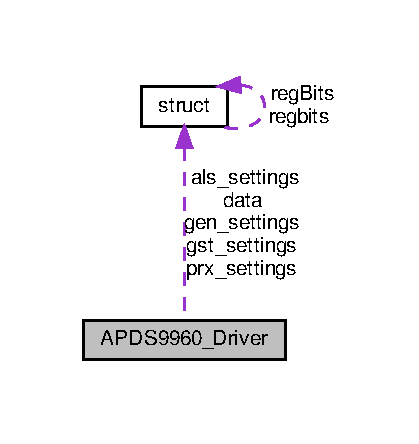
\includegraphics[width=201pt]{structAPDS9960__Driver__coll__graph}
\end{center}
\end{figure}
\subsection*{Public Attributes}
\begin{DoxyCompactItemize}
\item 
\mbox{\Hypertarget{structAPDS9960__Driver_a5706f944c7150a6908dbb382ee774cd6}\label{structAPDS9960__Driver_a5706f944c7150a6908dbb382ee774cd6}} 
\hyperlink{vl53l0x__types_8h_aba7bc1797add20fe3efdf37ced1182c5}{uint8\+\_\+t} {\bfseries bus}
\item 
\mbox{\Hypertarget{structAPDS9960__Driver_ad6ce95140873f0ed5e3bbf834595cbe7}\label{structAPDS9960__Driver_ad6ce95140873f0ed5e3bbf834595cbe7}} 
\hyperlink{vl53l0x__types_8h_aba7bc1797add20fe3efdf37ced1182c5}{uint8\+\_\+t} {\bfseries addr}
\item 
\mbox{\Hypertarget{structAPDS9960__Driver_ab764a56d9483a0f79f32c7f436aa8c4d}\label{structAPDS9960__Driver_ab764a56d9483a0f79f32c7f436aa8c4d}} 
bool {\bfseries intr\+\_\+en}
\item 
\mbox{\Hypertarget{structAPDS9960__Driver_ae954e4fa53a890e1c7c616f44b32d259}\label{structAPDS9960__Driver_ae954e4fa53a890e1c7c616f44b32d259}} 
gpio\+\_\+num\+\_\+t {\bfseries intr\+\_\+pin}
\item 
\mbox{\Hypertarget{structAPDS9960__Driver_a34f4d013dcbb5e0f83267d7cc9a75d34}\label{structAPDS9960__Driver_a34f4d013dcbb5e0f83267d7cc9a75d34}} 
\hyperlink{structgst__settings__t}{gst\+\_\+settings\+\_\+t} {\bfseries gst\+\_\+settings}
\item 
\mbox{\Hypertarget{structAPDS9960__Driver_a5a40dd89f78e16cd964a538395559d0c}\label{structAPDS9960__Driver_a5a40dd89f78e16cd964a538395559d0c}} 
\hyperlink{structprx__settings__t}{prx\+\_\+settings\+\_\+t} {\bfseries prx\+\_\+settings}
\item 
\mbox{\Hypertarget{structAPDS9960__Driver_ae53c09a13524750c25ee9f3c3dfe740a}\label{structAPDS9960__Driver_ae53c09a13524750c25ee9f3c3dfe740a}} 
\hyperlink{structals__settings__t}{als\+\_\+settings\+\_\+t} {\bfseries als\+\_\+settings}
\item 
\mbox{\Hypertarget{structAPDS9960__Driver_a3ce432690f1b2dc436fedb68443c3cb4}\label{structAPDS9960__Driver_a3ce432690f1b2dc436fedb68443c3cb4}} 
\hyperlink{structgen__settings__t}{gen\+\_\+settings\+\_\+t} {\bfseries gen\+\_\+settings}
\item 
\mbox{\Hypertarget{structAPDS9960__Driver_a4a660d3a469157e68f69ced004bee138}\label{structAPDS9960__Driver_a4a660d3a469157e68f69ced004bee138}} 
\hyperlink{structapds__data__t}{apds\+\_\+data\+\_\+t} {\bfseries data}
\item 
\mbox{\Hypertarget{structAPDS9960__Driver_a2335b853e3a6f2f3c3abd21d4bad28c3}\label{structAPDS9960__Driver_a2335b853e3a6f2f3c3abd21d4bad28c3}} 
Task\+Handle\+\_\+t {\bfseries t\+\_\+handle}
\end{DoxyCompactItemize}


The documentation for this struct was generated from the following file\+:\begin{DoxyCompactItemize}
\item 
A\+P\+D\+S9960\+\_\+\+Driver/A\+P\+D\+S9960\+\_\+\+Driver.\+h\end{DoxyCompactItemize}

\hypertarget{structAPDS9960__GST__Settings}{}\section{A\+P\+D\+S9960\+\_\+\+G\+S\+T\+\_\+\+Settings Struct Reference}
\label{structAPDS9960__GST__Settings}\index{A\+P\+D\+S9960\+\_\+\+G\+S\+T\+\_\+\+Settings@{A\+P\+D\+S9960\+\_\+\+G\+S\+T\+\_\+\+Settings}}
\subsection*{Public Attributes}
\begin{DoxyCompactItemize}
\item 
\mbox{\Hypertarget{structAPDS9960__GST__Settings_a22b1891a0b87f0fb032b8873619c23f6}\label{structAPDS9960__GST__Settings_a22b1891a0b87f0fb032b8873619c23f6}} 
bool {\bfseries gst\+\_\+en}
\item 
\mbox{\Hypertarget{structAPDS9960__GST__Settings_acc5de6a7e15d4d9317c7875366616df2}\label{structAPDS9960__GST__Settings_acc5de6a7e15d4d9317c7875366616df2}} 
bool {\bfseries gmode}
\item 
\mbox{\Hypertarget{structAPDS9960__GST__Settings_a6d4ee381934228214c7b6600295fd01a}\label{structAPDS9960__GST__Settings_a6d4ee381934228214c7b6600295fd01a}} 
bool {\bfseries low\+\_\+pwr\+\_\+clk}
\item 
\mbox{\Hypertarget{structAPDS9960__GST__Settings_af310644079e508cee68becc26b60cabc}\label{structAPDS9960__GST__Settings_af310644079e508cee68becc26b60cabc}} 
bool {\bfseries gst\+\_\+int\+\_\+en}
\item 
\mbox{\Hypertarget{structAPDS9960__GST__Settings_a98e34db047aa71fb1b50de1a2221583c}\label{structAPDS9960__GST__Settings_a98e34db047aa71fb1b50de1a2221583c}} 
\hyperlink{vl53l0x__types_8h_aba7bc1797add20fe3efdf37ced1182c5}{uint8\+\_\+t} {\bfseries gst\+\_\+thresh\+\_\+entr}
\item 
\mbox{\Hypertarget{structAPDS9960__GST__Settings_ac4328cd9a486f3f17b061cd32844b531}\label{structAPDS9960__GST__Settings_ac4328cd9a486f3f17b061cd32844b531}} 
\hyperlink{vl53l0x__types_8h_aba7bc1797add20fe3efdf37ced1182c5}{uint8\+\_\+t} {\bfseries gst\+\_\+thresh\+\_\+exit}
\item 
\mbox{\Hypertarget{structAPDS9960__GST__Settings_a7c7650ca944df56abd67922d05acb411}\label{structAPDS9960__GST__Settings_a7c7650ca944df56abd67922d05acb411}} 
\hyperlink{vl53l0x__types_8h_aba7bc1797add20fe3efdf37ced1182c5}{uint8\+\_\+t} {\bfseries gst\+\_\+gain\+\_\+ctrl}
\item 
\mbox{\Hypertarget{structAPDS9960__GST__Settings_a9ede316080e157e81e053bdd825adac5}\label{structAPDS9960__GST__Settings_a9ede316080e157e81e053bdd825adac5}} 
\hyperlink{vl53l0x__types_8h_aba7bc1797add20fe3efdf37ced1182c5}{uint8\+\_\+t} {\bfseries gst\+\_\+exit\+\_\+persist}
\item 
\mbox{\Hypertarget{structAPDS9960__GST__Settings_a0fa5f9f636e18d4451d47a2ec602a01f}\label{structAPDS9960__GST__Settings_a0fa5f9f636e18d4451d47a2ec602a01f}} 
\hyperlink{vl53l0x__types_8h_aba7bc1797add20fe3efdf37ced1182c5}{uint8\+\_\+t} {\bfseries gst\+\_\+exit\+\_\+mask}
\item 
\mbox{\Hypertarget{structAPDS9960__GST__Settings_ab28dae96309bba20140abf3a6ed02930}\label{structAPDS9960__GST__Settings_ab28dae96309bba20140abf3a6ed02930}} 
\hyperlink{vl53l0x__types_8h_aba7bc1797add20fe3efdf37ced1182c5}{uint8\+\_\+t} {\bfseries gst\+\_\+led\+\_\+drive\+\_\+str}
\item 
\mbox{\Hypertarget{structAPDS9960__GST__Settings_a40152fc0233d915be18312af84257bf9}\label{structAPDS9960__GST__Settings_a40152fc0233d915be18312af84257bf9}} 
\hyperlink{vl53l0x__types_8h_aba7bc1797add20fe3efdf37ced1182c5}{uint8\+\_\+t} {\bfseries gst\+\_\+wait\+\_\+time}
\item 
\mbox{\Hypertarget{structAPDS9960__GST__Settings_adab7e5c3d41b74a8ee94f292e0292ce4}\label{structAPDS9960__GST__Settings_adab7e5c3d41b74a8ee94f292e0292ce4}} 
\hyperlink{vl53l0x__types_8h_aba7bc1797add20fe3efdf37ced1182c5}{uint8\+\_\+t} {\bfseries gst\+\_\+satr}
\item 
\mbox{\Hypertarget{structAPDS9960__GST__Settings_a73dd0640450af1eebd164a060503ea20}\label{structAPDS9960__GST__Settings_a73dd0640450af1eebd164a060503ea20}} 
\hyperlink{vl53l0x__types_8h_aba7bc1797add20fe3efdf37ced1182c5}{uint8\+\_\+t} {\bfseries gst\+\_\+pulse\+\_\+cnt}
\item 
\mbox{\Hypertarget{structAPDS9960__GST__Settings_af21f71fc4e8d2c7b5187c892738f94d7}\label{structAPDS9960__GST__Settings_af21f71fc4e8d2c7b5187c892738f94d7}} 
\hyperlink{vl53l0x__types_8h_aba7bc1797add20fe3efdf37ced1182c5}{uint8\+\_\+t} {\bfseries gst\+\_\+pulse\+\_\+len}
\item 
\mbox{\Hypertarget{structAPDS9960__GST__Settings_aa9f84c8c2be08236fdec2dc2482f16b0}\label{structAPDS9960__GST__Settings_aa9f84c8c2be08236fdec2dc2482f16b0}} 
\hyperlink{vl53l0x__types_8h_aba7bc1797add20fe3efdf37ced1182c5}{uint8\+\_\+t} {\bfseries gst\+\_\+dir\+\_\+select}
\item 
\mbox{\Hypertarget{structAPDS9960__GST__Settings_a14ac7d5ca87b7d4d26e51a66a43aed63}\label{structAPDS9960__GST__Settings_a14ac7d5ca87b7d4d26e51a66a43aed63}} 
\hyperlink{vl53l0x__types_8h_aba7bc1797add20fe3efdf37ced1182c5}{uint8\+\_\+t} {\bfseries gst\+\_\+fifo\+\_\+thresh}
\item 
\mbox{\Hypertarget{structAPDS9960__GST__Settings_a714c2766496a3ed08fe1621ba9403905}\label{structAPDS9960__GST__Settings_a714c2766496a3ed08fe1621ba9403905}} 
bool {\bfseries gst\+\_\+ovr}
\item 
\mbox{\Hypertarget{structAPDS9960__GST__Settings_a81de6373bbe66c6d15c2c968c222201d}\label{structAPDS9960__GST__Settings_a81de6373bbe66c6d15c2c968c222201d}} 
bool {\bfseries gst\+\_\+fifo\+\_\+rdy}
\item 
\mbox{\Hypertarget{structAPDS9960__GST__Settings_aeee3d433e79e039a2eaaa91abe6c237a}\label{structAPDS9960__GST__Settings_aeee3d433e79e039a2eaaa91abe6c237a}} 
\hyperlink{vl53l0x__types_8h_aba7bc1797add20fe3efdf37ced1182c5}{uint8\+\_\+t} {\bfseries fifo\+\_\+pkts\+\_\+read}
\item 
\mbox{\Hypertarget{structAPDS9960__GST__Settings_aaab006b6a7717d09c505eed74cd1f7d4}\label{structAPDS9960__GST__Settings_aaab006b6a7717d09c505eed74cd1f7d4}} 
apds\+\_\+swipe\+\_\+t {\bfseries last\+\_\+swipe}
\end{DoxyCompactItemize}


The documentation for this struct was generated from the following file\+:\begin{DoxyCompactItemize}
\item 
A\+P\+D\+S9960\+\_\+\+Driver/A\+P\+D\+S9960\+\_\+\+Driver.\+h\end{DoxyCompactItemize}

\hypertarget{structAPDS9960__PRX__Settings}{}\section{A\+P\+D\+S9960\+\_\+\+P\+R\+X\+\_\+\+Settings Struct Reference}
\label{structAPDS9960__PRX__Settings}\index{A\+P\+D\+S9960\+\_\+\+P\+R\+X\+\_\+\+Settings@{A\+P\+D\+S9960\+\_\+\+P\+R\+X\+\_\+\+Settings}}
\subsection*{Public Attributes}
\begin{DoxyCompactItemize}
\item 
bool \hyperlink{structAPDS9960__PRX__Settings_af5eaa566c4e9a0acfcea99e9d66ff1ce}{prx\+\_\+en}
\item 
bool \hyperlink{structAPDS9960__PRX__Settings_ac60827f0df46f3b85d65ba72c2f8083b}{prox\+\_\+intr\+\_\+en}
\item 
bool \hyperlink{structAPDS9960__PRX__Settings_aa50ba09a8a7fedf583a32594c000900c}{prox\+\_\+satr\+\_\+int\+\_\+en}
\item 
bool \hyperlink{structAPDS9960__PRX__Settings_a5bab20fc71f543fd4f998f25f7a8d49d}{prox\+\_\+gain\+\_\+comp\+\_\+en}
\item 
\hyperlink{vl53l0x__types_8h_aba7bc1797add20fe3efdf37ced1182c5}{uint8\+\_\+t} \hyperlink{structAPDS9960__PRX__Settings_a6444eabe6fb90f8530db05303b464070}{prox\+\_\+thresh\+\_\+l}
\item 
\hyperlink{vl53l0x__types_8h_aba7bc1797add20fe3efdf37ced1182c5}{uint8\+\_\+t} \hyperlink{structAPDS9960__PRX__Settings_a24a23f24988adc6c2aa6ba3124d5f0e1}{prox\+\_\+thresh\+\_\+h}
\item 
\hyperlink{vl53l0x__types_8h_aba7bc1797add20fe3efdf37ced1182c5}{uint8\+\_\+t} \hyperlink{structAPDS9960__PRX__Settings_ae78c2262acc73db5fce3609b1e2f5f21}{prox\+\_\+gain}
\item 
\hyperlink{vl53l0x__types_8h_aba7bc1797add20fe3efdf37ced1182c5}{uint8\+\_\+t} \hyperlink{structAPDS9960__PRX__Settings_a09355063e89505fd8fca4ad1b6a4c80f}{prox\+\_\+led\+\_\+en\+\_\+mask}
\item 
\hyperlink{vl53l0x__types_8h_aba7bc1797add20fe3efdf37ced1182c5}{uint8\+\_\+t} \hyperlink{structAPDS9960__PRX__Settings_abce5736db684f41e5bcec51abc0f4155}{led\+\_\+pulse\+\_\+n}
\item 
\hyperlink{vl53l0x__types_8h_aba7bc1797add20fe3efdf37ced1182c5}{uint8\+\_\+t} \hyperlink{structAPDS9960__PRX__Settings_a4653b89fc667820b09276cb902708e37}{prox\+\_\+perist\+\_\+cycles}
\item 
prx\+\_\+ledtime\+\_\+t \hyperlink{structAPDS9960__PRX__Settings_af20ad1811d5d4c376b740a2708aea267}{ledtime}
\end{DoxyCompactItemize}


\subsection{Member Data Documentation}
\mbox{\Hypertarget{structAPDS9960__PRX__Settings_abce5736db684f41e5bcec51abc0f4155}\label{structAPDS9960__PRX__Settings_abce5736db684f41e5bcec51abc0f4155}} 
\index{A\+P\+D\+S9960\+\_\+\+P\+R\+X\+\_\+\+Settings@{A\+P\+D\+S9960\+\_\+\+P\+R\+X\+\_\+\+Settings}!led\+\_\+pulse\+\_\+n@{led\+\_\+pulse\+\_\+n}}
\index{led\+\_\+pulse\+\_\+n@{led\+\_\+pulse\+\_\+n}!A\+P\+D\+S9960\+\_\+\+P\+R\+X\+\_\+\+Settings@{A\+P\+D\+S9960\+\_\+\+P\+R\+X\+\_\+\+Settings}}
\subsubsection{\texorpdfstring{led\+\_\+pulse\+\_\+n}{led\_pulse\_n}}
{\footnotesize\ttfamily \hyperlink{vl53l0x__types_8h_aba7bc1797add20fe3efdf37ced1182c5}{uint8\+\_\+t} A\+P\+D\+S9960\+\_\+\+P\+R\+X\+\_\+\+Settings\+::led\+\_\+pulse\+\_\+n}

proximity led pulses per measure \mbox{\Hypertarget{structAPDS9960__PRX__Settings_af20ad1811d5d4c376b740a2708aea267}\label{structAPDS9960__PRX__Settings_af20ad1811d5d4c376b740a2708aea267}} 
\index{A\+P\+D\+S9960\+\_\+\+P\+R\+X\+\_\+\+Settings@{A\+P\+D\+S9960\+\_\+\+P\+R\+X\+\_\+\+Settings}!ledtime@{ledtime}}
\index{ledtime@{ledtime}!A\+P\+D\+S9960\+\_\+\+P\+R\+X\+\_\+\+Settings@{A\+P\+D\+S9960\+\_\+\+P\+R\+X\+\_\+\+Settings}}
\subsubsection{\texorpdfstring{ledtime}{ledtime}}
{\footnotesize\ttfamily prx\+\_\+ledtime\+\_\+t A\+P\+D\+S9960\+\_\+\+P\+R\+X\+\_\+\+Settings\+::ledtime}

proximity led on-\/time \mbox{\Hypertarget{structAPDS9960__PRX__Settings_ae78c2262acc73db5fce3609b1e2f5f21}\label{structAPDS9960__PRX__Settings_ae78c2262acc73db5fce3609b1e2f5f21}} 
\index{A\+P\+D\+S9960\+\_\+\+P\+R\+X\+\_\+\+Settings@{A\+P\+D\+S9960\+\_\+\+P\+R\+X\+\_\+\+Settings}!prox\+\_\+gain@{prox\+\_\+gain}}
\index{prox\+\_\+gain@{prox\+\_\+gain}!A\+P\+D\+S9960\+\_\+\+P\+R\+X\+\_\+\+Settings@{A\+P\+D\+S9960\+\_\+\+P\+R\+X\+\_\+\+Settings}}
\subsubsection{\texorpdfstring{prox\+\_\+gain}{prox\_gain}}
{\footnotesize\ttfamily \hyperlink{vl53l0x__types_8h_aba7bc1797add20fe3efdf37ced1182c5}{uint8\+\_\+t} A\+P\+D\+S9960\+\_\+\+P\+R\+X\+\_\+\+Settings\+::prox\+\_\+gain}

proximity measurement gain \mbox{\Hypertarget{structAPDS9960__PRX__Settings_a5bab20fc71f543fd4f998f25f7a8d49d}\label{structAPDS9960__PRX__Settings_a5bab20fc71f543fd4f998f25f7a8d49d}} 
\index{A\+P\+D\+S9960\+\_\+\+P\+R\+X\+\_\+\+Settings@{A\+P\+D\+S9960\+\_\+\+P\+R\+X\+\_\+\+Settings}!prox\+\_\+gain\+\_\+comp\+\_\+en@{prox\+\_\+gain\+\_\+comp\+\_\+en}}
\index{prox\+\_\+gain\+\_\+comp\+\_\+en@{prox\+\_\+gain\+\_\+comp\+\_\+en}!A\+P\+D\+S9960\+\_\+\+P\+R\+X\+\_\+\+Settings@{A\+P\+D\+S9960\+\_\+\+P\+R\+X\+\_\+\+Settings}}
\subsubsection{\texorpdfstring{prox\+\_\+gain\+\_\+comp\+\_\+en}{prox\_gain\_comp\_en}}
{\footnotesize\ttfamily bool A\+P\+D\+S9960\+\_\+\+P\+R\+X\+\_\+\+Settings\+::prox\+\_\+gain\+\_\+comp\+\_\+en}

D\+E\+P\+R\+E\+C\+A\+T\+ED \mbox{\Hypertarget{structAPDS9960__PRX__Settings_ac60827f0df46f3b85d65ba72c2f8083b}\label{structAPDS9960__PRX__Settings_ac60827f0df46f3b85d65ba72c2f8083b}} 
\index{A\+P\+D\+S9960\+\_\+\+P\+R\+X\+\_\+\+Settings@{A\+P\+D\+S9960\+\_\+\+P\+R\+X\+\_\+\+Settings}!prox\+\_\+intr\+\_\+en@{prox\+\_\+intr\+\_\+en}}
\index{prox\+\_\+intr\+\_\+en@{prox\+\_\+intr\+\_\+en}!A\+P\+D\+S9960\+\_\+\+P\+R\+X\+\_\+\+Settings@{A\+P\+D\+S9960\+\_\+\+P\+R\+X\+\_\+\+Settings}}
\subsubsection{\texorpdfstring{prox\+\_\+intr\+\_\+en}{prox\_intr\_en}}
{\footnotesize\ttfamily bool A\+P\+D\+S9960\+\_\+\+P\+R\+X\+\_\+\+Settings\+::prox\+\_\+intr\+\_\+en}

proximity interrupt enabled \mbox{\Hypertarget{structAPDS9960__PRX__Settings_a09355063e89505fd8fca4ad1b6a4c80f}\label{structAPDS9960__PRX__Settings_a09355063e89505fd8fca4ad1b6a4c80f}} 
\index{A\+P\+D\+S9960\+\_\+\+P\+R\+X\+\_\+\+Settings@{A\+P\+D\+S9960\+\_\+\+P\+R\+X\+\_\+\+Settings}!prox\+\_\+led\+\_\+en\+\_\+mask@{prox\+\_\+led\+\_\+en\+\_\+mask}}
\index{prox\+\_\+led\+\_\+en\+\_\+mask@{prox\+\_\+led\+\_\+en\+\_\+mask}!A\+P\+D\+S9960\+\_\+\+P\+R\+X\+\_\+\+Settings@{A\+P\+D\+S9960\+\_\+\+P\+R\+X\+\_\+\+Settings}}
\subsubsection{\texorpdfstring{prox\+\_\+led\+\_\+en\+\_\+mask}{prox\_led\_en\_mask}}
{\footnotesize\ttfamily \hyperlink{vl53l0x__types_8h_aba7bc1797add20fe3efdf37ced1182c5}{uint8\+\_\+t} A\+P\+D\+S9960\+\_\+\+P\+R\+X\+\_\+\+Settings\+::prox\+\_\+led\+\_\+en\+\_\+mask}

proximity led enabled mask \mbox{\Hypertarget{structAPDS9960__PRX__Settings_a4653b89fc667820b09276cb902708e37}\label{structAPDS9960__PRX__Settings_a4653b89fc667820b09276cb902708e37}} 
\index{A\+P\+D\+S9960\+\_\+\+P\+R\+X\+\_\+\+Settings@{A\+P\+D\+S9960\+\_\+\+P\+R\+X\+\_\+\+Settings}!prox\+\_\+perist\+\_\+cycles@{prox\+\_\+perist\+\_\+cycles}}
\index{prox\+\_\+perist\+\_\+cycles@{prox\+\_\+perist\+\_\+cycles}!A\+P\+D\+S9960\+\_\+\+P\+R\+X\+\_\+\+Settings@{A\+P\+D\+S9960\+\_\+\+P\+R\+X\+\_\+\+Settings}}
\subsubsection{\texorpdfstring{prox\+\_\+perist\+\_\+cycles}{prox\_perist\_cycles}}
{\footnotesize\ttfamily \hyperlink{vl53l0x__types_8h_aba7bc1797add20fe3efdf37ced1182c5}{uint8\+\_\+t} A\+P\+D\+S9960\+\_\+\+P\+R\+X\+\_\+\+Settings\+::prox\+\_\+perist\+\_\+cycles}

proximity exit persistence \mbox{\Hypertarget{structAPDS9960__PRX__Settings_aa50ba09a8a7fedf583a32594c000900c}\label{structAPDS9960__PRX__Settings_aa50ba09a8a7fedf583a32594c000900c}} 
\index{A\+P\+D\+S9960\+\_\+\+P\+R\+X\+\_\+\+Settings@{A\+P\+D\+S9960\+\_\+\+P\+R\+X\+\_\+\+Settings}!prox\+\_\+satr\+\_\+int\+\_\+en@{prox\+\_\+satr\+\_\+int\+\_\+en}}
\index{prox\+\_\+satr\+\_\+int\+\_\+en@{prox\+\_\+satr\+\_\+int\+\_\+en}!A\+P\+D\+S9960\+\_\+\+P\+R\+X\+\_\+\+Settings@{A\+P\+D\+S9960\+\_\+\+P\+R\+X\+\_\+\+Settings}}
\subsubsection{\texorpdfstring{prox\+\_\+satr\+\_\+int\+\_\+en}{prox\_satr\_int\_en}}
{\footnotesize\ttfamily bool A\+P\+D\+S9960\+\_\+\+P\+R\+X\+\_\+\+Settings\+::prox\+\_\+satr\+\_\+int\+\_\+en}

interrupt if proximity saturated \mbox{\Hypertarget{structAPDS9960__PRX__Settings_a24a23f24988adc6c2aa6ba3124d5f0e1}\label{structAPDS9960__PRX__Settings_a24a23f24988adc6c2aa6ba3124d5f0e1}} 
\index{A\+P\+D\+S9960\+\_\+\+P\+R\+X\+\_\+\+Settings@{A\+P\+D\+S9960\+\_\+\+P\+R\+X\+\_\+\+Settings}!prox\+\_\+thresh\+\_\+h@{prox\+\_\+thresh\+\_\+h}}
\index{prox\+\_\+thresh\+\_\+h@{prox\+\_\+thresh\+\_\+h}!A\+P\+D\+S9960\+\_\+\+P\+R\+X\+\_\+\+Settings@{A\+P\+D\+S9960\+\_\+\+P\+R\+X\+\_\+\+Settings}}
\subsubsection{\texorpdfstring{prox\+\_\+thresh\+\_\+h}{prox\_thresh\_h}}
{\footnotesize\ttfamily \hyperlink{vl53l0x__types_8h_aba7bc1797add20fe3efdf37ced1182c5}{uint8\+\_\+t} A\+P\+D\+S9960\+\_\+\+P\+R\+X\+\_\+\+Settings\+::prox\+\_\+thresh\+\_\+h}

proximity threshold upper limit \mbox{\Hypertarget{structAPDS9960__PRX__Settings_a6444eabe6fb90f8530db05303b464070}\label{structAPDS9960__PRX__Settings_a6444eabe6fb90f8530db05303b464070}} 
\index{A\+P\+D\+S9960\+\_\+\+P\+R\+X\+\_\+\+Settings@{A\+P\+D\+S9960\+\_\+\+P\+R\+X\+\_\+\+Settings}!prox\+\_\+thresh\+\_\+l@{prox\+\_\+thresh\+\_\+l}}
\index{prox\+\_\+thresh\+\_\+l@{prox\+\_\+thresh\+\_\+l}!A\+P\+D\+S9960\+\_\+\+P\+R\+X\+\_\+\+Settings@{A\+P\+D\+S9960\+\_\+\+P\+R\+X\+\_\+\+Settings}}
\subsubsection{\texorpdfstring{prox\+\_\+thresh\+\_\+l}{prox\_thresh\_l}}
{\footnotesize\ttfamily \hyperlink{vl53l0x__types_8h_aba7bc1797add20fe3efdf37ced1182c5}{uint8\+\_\+t} A\+P\+D\+S9960\+\_\+\+P\+R\+X\+\_\+\+Settings\+::prox\+\_\+thresh\+\_\+l}

proximity threshold lower limit \mbox{\Hypertarget{structAPDS9960__PRX__Settings_af5eaa566c4e9a0acfcea99e9d66ff1ce}\label{structAPDS9960__PRX__Settings_af5eaa566c4e9a0acfcea99e9d66ff1ce}} 
\index{A\+P\+D\+S9960\+\_\+\+P\+R\+X\+\_\+\+Settings@{A\+P\+D\+S9960\+\_\+\+P\+R\+X\+\_\+\+Settings}!prx\+\_\+en@{prx\+\_\+en}}
\index{prx\+\_\+en@{prx\+\_\+en}!A\+P\+D\+S9960\+\_\+\+P\+R\+X\+\_\+\+Settings@{A\+P\+D\+S9960\+\_\+\+P\+R\+X\+\_\+\+Settings}}
\subsubsection{\texorpdfstring{prx\+\_\+en}{prx\_en}}
{\footnotesize\ttfamily bool A\+P\+D\+S9960\+\_\+\+P\+R\+X\+\_\+\+Settings\+::prx\+\_\+en}

Proximity engine enabled 

The documentation for this struct was generated from the following file\+:\begin{DoxyCompactItemize}
\item 
A\+P\+D\+S9960\+\_\+\+Driver/A\+P\+D\+S9960\+\_\+\+Driver.\+h\end{DoxyCompactItemize}

\hypertarget{structapds__data__t}{}\section{apds\+\_\+data\+\_\+t Struct Reference}
\label{structapds__data__t}\index{apds\+\_\+data\+\_\+t@{apds\+\_\+data\+\_\+t}}


\hyperlink{structThe}{The} latest fifo data.  




{\ttfamily \#include $<$A\+P\+D\+S9960\+\_\+\+Driver.\+h$>$}



\subsection{Detailed Description}
\hyperlink{structThe}{The} latest fifo data. 

The documentation for this struct was generated from the following file\+:\begin{DoxyCompactItemize}
\item 
A\+P\+D\+S9960\+\_\+\+Driver/A\+P\+D\+S9960\+\_\+\+Driver.\+h\end{DoxyCompactItemize}

\hypertarget{structAPDS__GeneralSettings}{}\section{A\+P\+D\+S\+\_\+\+General\+Settings Struct Reference}
\label{structAPDS__GeneralSettings}\index{A\+P\+D\+S\+\_\+\+General\+Settings@{A\+P\+D\+S\+\_\+\+General\+Settings}}
\subsection*{Public Attributes}
\begin{DoxyCompactItemize}
\item 
bool \hyperlink{structAPDS__GeneralSettings_ad2a30d2b8de189e172590761d17faf4c}{sleep\+\_\+after\+\_\+intr}
\item 
bool \hyperlink{structAPDS__GeneralSettings_a9ea5752f59abeea31c54a59621f1e8e7}{pwr\+\_\+on}
\item 
\hyperlink{vl53l0x__types_8h_a435d1572bf3f880d55459d9805097f62}{uint32\+\_\+t} \hyperlink{structAPDS__GeneralSettings_a01d37b5bd42dab254fd9701492784a03}{wait\+\_\+time\+\_\+ms}
\item 
\hyperlink{vl53l0x__types_8h_aba7bc1797add20fe3efdf37ced1182c5}{uint8\+\_\+t} \hyperlink{structAPDS__GeneralSettings_ac782ac2109c3302dcdb35d26ad2ce664}{wait\+\_\+time}
\item 
bool \hyperlink{structAPDS__GeneralSettings_ad5bb9912a9cb4653257113d164b56b54}{wait\+\_\+long\+\_\+en}
\item 
bool \hyperlink{structAPDS__GeneralSettings_ab298e8bcba856af83c12c0a356341ecf}{wait\+\_\+en}
\end{DoxyCompactItemize}


\subsection{Member Data Documentation}
\mbox{\Hypertarget{structAPDS__GeneralSettings_a9ea5752f59abeea31c54a59621f1e8e7}\label{structAPDS__GeneralSettings_a9ea5752f59abeea31c54a59621f1e8e7}} 
\index{A\+P\+D\+S\+\_\+\+General\+Settings@{A\+P\+D\+S\+\_\+\+General\+Settings}!pwr\+\_\+on@{pwr\+\_\+on}}
\index{pwr\+\_\+on@{pwr\+\_\+on}!A\+P\+D\+S\+\_\+\+General\+Settings@{A\+P\+D\+S\+\_\+\+General\+Settings}}
\subsubsection{\texorpdfstring{pwr\+\_\+on}{pwr\_on}}
{\footnotesize\ttfamily bool A\+P\+D\+S\+\_\+\+General\+Settings\+::pwr\+\_\+on}

power on! \mbox{\Hypertarget{structAPDS__GeneralSettings_ad2a30d2b8de189e172590761d17faf4c}\label{structAPDS__GeneralSettings_ad2a30d2b8de189e172590761d17faf4c}} 
\index{A\+P\+D\+S\+\_\+\+General\+Settings@{A\+P\+D\+S\+\_\+\+General\+Settings}!sleep\+\_\+after\+\_\+intr@{sleep\+\_\+after\+\_\+intr}}
\index{sleep\+\_\+after\+\_\+intr@{sleep\+\_\+after\+\_\+intr}!A\+P\+D\+S\+\_\+\+General\+Settings@{A\+P\+D\+S\+\_\+\+General\+Settings}}
\subsubsection{\texorpdfstring{sleep\+\_\+after\+\_\+intr}{sleep\_after\_intr}}
{\footnotesize\ttfamily bool A\+P\+D\+S\+\_\+\+General\+Settings\+::sleep\+\_\+after\+\_\+intr}

sleep after interrupt enabled \mbox{\Hypertarget{structAPDS__GeneralSettings_ab298e8bcba856af83c12c0a356341ecf}\label{structAPDS__GeneralSettings_ab298e8bcba856af83c12c0a356341ecf}} 
\index{A\+P\+D\+S\+\_\+\+General\+Settings@{A\+P\+D\+S\+\_\+\+General\+Settings}!wait\+\_\+en@{wait\+\_\+en}}
\index{wait\+\_\+en@{wait\+\_\+en}!A\+P\+D\+S\+\_\+\+General\+Settings@{A\+P\+D\+S\+\_\+\+General\+Settings}}
\subsubsection{\texorpdfstring{wait\+\_\+en}{wait\_en}}
{\footnotesize\ttfamily bool A\+P\+D\+S\+\_\+\+General\+Settings\+::wait\+\_\+en}

wait enabled \mbox{\Hypertarget{structAPDS__GeneralSettings_ad5bb9912a9cb4653257113d164b56b54}\label{structAPDS__GeneralSettings_ad5bb9912a9cb4653257113d164b56b54}} 
\index{A\+P\+D\+S\+\_\+\+General\+Settings@{A\+P\+D\+S\+\_\+\+General\+Settings}!wait\+\_\+long\+\_\+en@{wait\+\_\+long\+\_\+en}}
\index{wait\+\_\+long\+\_\+en@{wait\+\_\+long\+\_\+en}!A\+P\+D\+S\+\_\+\+General\+Settings@{A\+P\+D\+S\+\_\+\+General\+Settings}}
\subsubsection{\texorpdfstring{wait\+\_\+long\+\_\+en}{wait\_long\_en}}
{\footnotesize\ttfamily bool A\+P\+D\+S\+\_\+\+General\+Settings\+::wait\+\_\+long\+\_\+en}

longer waits enabled \mbox{\Hypertarget{structAPDS__GeneralSettings_ac782ac2109c3302dcdb35d26ad2ce664}\label{structAPDS__GeneralSettings_ac782ac2109c3302dcdb35d26ad2ce664}} 
\index{A\+P\+D\+S\+\_\+\+General\+Settings@{A\+P\+D\+S\+\_\+\+General\+Settings}!wait\+\_\+time@{wait\+\_\+time}}
\index{wait\+\_\+time@{wait\+\_\+time}!A\+P\+D\+S\+\_\+\+General\+Settings@{A\+P\+D\+S\+\_\+\+General\+Settings}}
\subsubsection{\texorpdfstring{wait\+\_\+time}{wait\_time}}
{\footnotesize\ttfamily \hyperlink{vl53l0x__types_8h_aba7bc1797add20fe3efdf37ced1182c5}{uint8\+\_\+t} A\+P\+D\+S\+\_\+\+General\+Settings\+::wait\+\_\+time}

value set to wait register \mbox{\Hypertarget{structAPDS__GeneralSettings_a01d37b5bd42dab254fd9701492784a03}\label{structAPDS__GeneralSettings_a01d37b5bd42dab254fd9701492784a03}} 
\index{A\+P\+D\+S\+\_\+\+General\+Settings@{A\+P\+D\+S\+\_\+\+General\+Settings}!wait\+\_\+time\+\_\+ms@{wait\+\_\+time\+\_\+ms}}
\index{wait\+\_\+time\+\_\+ms@{wait\+\_\+time\+\_\+ms}!A\+P\+D\+S\+\_\+\+General\+Settings@{A\+P\+D\+S\+\_\+\+General\+Settings}}
\subsubsection{\texorpdfstring{wait\+\_\+time\+\_\+ms}{wait\_time\_ms}}
{\footnotesize\ttfamily \hyperlink{vl53l0x__types_8h_a435d1572bf3f880d55459d9805097f62}{uint32\+\_\+t} A\+P\+D\+S\+\_\+\+General\+Settings\+::wait\+\_\+time\+\_\+ms}

time to idle per cycle in ms(see datasheet for state machine) 

The documentation for this struct was generated from the following file\+:\begin{DoxyCompactItemize}
\item 
A\+P\+D\+S9960\+\_\+\+Driver/A\+P\+D\+S9960\+\_\+\+Driver.\+h\end{DoxyCompactItemize}

\hypertarget{structAPDS__Init}{}\section{A\+P\+D\+S\+\_\+\+Init Struct Reference}
\label{structAPDS__Init}\index{A\+P\+D\+S\+\_\+\+Init@{A\+P\+D\+S\+\_\+\+Init}}
\subsection*{Public Attributes}
\begin{DoxyCompactItemize}
\item 
\mbox{\Hypertarget{structAPDS__Init_a701992ac82c11149cc7836cb0b0e1027}\label{structAPDS__Init_a701992ac82c11149cc7836cb0b0e1027}} 
\hyperlink{vl53l0x__types_8h_aba7bc1797add20fe3efdf37ced1182c5}{uint8\+\_\+t} {\bfseries i2c\+\_\+bus}
\item 
gpio\+\_\+num\+\_\+t \hyperlink{structAPDS__Init_a387fbf2b939af62c370c8e1b51371df3}{intr\+\_\+pin}
\end{DoxyCompactItemize}


\subsection{Member Data Documentation}
\mbox{\Hypertarget{structAPDS__Init_a387fbf2b939af62c370c8e1b51371df3}\label{structAPDS__Init_a387fbf2b939af62c370c8e1b51371df3}} 
\index{A\+P\+D\+S\+\_\+\+Init@{A\+P\+D\+S\+\_\+\+Init}!intr\+\_\+pin@{intr\+\_\+pin}}
\index{intr\+\_\+pin@{intr\+\_\+pin}!A\+P\+D\+S\+\_\+\+Init@{A\+P\+D\+S\+\_\+\+Init}}
\subsubsection{\texorpdfstring{intr\+\_\+pin}{intr\_pin}}
{\footnotesize\ttfamily gpio\+\_\+num\+\_\+t A\+P\+D\+S\+\_\+\+Init\+::intr\+\_\+pin}

!$<$ i2c bus to use (should be initialised) 

The documentation for this struct was generated from the following file\+:\begin{DoxyCompactItemize}
\item 
A\+P\+D\+S9960\+\_\+\+Driver/A\+P\+D\+S9960\+\_\+\+Driver.\+h\end{DoxyCompactItemize}

\hypertarget{structapds__init__t}{}\section{apds\+\_\+init\+\_\+t Struct Reference}
\label{structapds__init__t}\index{apds\+\_\+init\+\_\+t@{apds\+\_\+init\+\_\+t}}


\hyperlink{structThe}{The} initialiser info for the A\+P\+DS driver.  




{\ttfamily \#include $<$A\+P\+D\+S9960\+\_\+\+Driver.\+h$>$}



\subsection{Detailed Description}
\hyperlink{structThe}{The} initialiser info for the A\+P\+DS driver. 

The documentation for this struct was generated from the following file\+:\begin{DoxyCompactItemize}
\item 
A\+P\+D\+S9960\+\_\+\+Driver/A\+P\+D\+S9960\+\_\+\+Driver.\+h\end{DoxyCompactItemize}

\hypertarget{structBM__CalibrationData}{}\section{B\+M\+\_\+\+Calibration\+Data Struct Reference}
\label{structBM__CalibrationData}\index{B\+M\+\_\+\+Calibration\+Data@{B\+M\+\_\+\+Calibration\+Data}}
\subsection*{Public Attributes}
\begin{DoxyCompactItemize}
\item 
\mbox{\Hypertarget{structBM__CalibrationData_a1f0f0ad502c7ad302d1d75c41897326c}\label{structBM__CalibrationData_a1f0f0ad502c7ad302d1d75c41897326c}} 
\hyperlink{vl53l0x__types_8h_a273cf69d639a59973b6019625df33e30}{uint16\+\_\+t} {\bfseries dig\+\_\+\+T1}
\item 
\mbox{\Hypertarget{structBM__CalibrationData_a5fa3b1681b52b9f3ef94c4600b464f24}\label{structBM__CalibrationData_a5fa3b1681b52b9f3ef94c4600b464f24}} 
\hyperlink{vl53l0x__types_8h_aa343fa3b3d06292b959ffdd4c4703b06}{int16\+\_\+t} {\bfseries dig\+\_\+\+T2}
\item 
\mbox{\Hypertarget{structBM__CalibrationData_a6a95bd8dc6e4750b4370c5277e762621}\label{structBM__CalibrationData_a6a95bd8dc6e4750b4370c5277e762621}} 
\hyperlink{vl53l0x__types_8h_aa343fa3b3d06292b959ffdd4c4703b06}{int16\+\_\+t} {\bfseries dig\+\_\+\+T3}
\item 
\mbox{\Hypertarget{structBM__CalibrationData_a229d9c150036f8013f98270f625c365b}\label{structBM__CalibrationData_a229d9c150036f8013f98270f625c365b}} 
\hyperlink{vl53l0x__types_8h_a273cf69d639a59973b6019625df33e30}{uint16\+\_\+t} {\bfseries dig\+\_\+\+P1}
\item 
\mbox{\Hypertarget{structBM__CalibrationData_a76509932ead2ddca230f134e9b50845b}\label{structBM__CalibrationData_a76509932ead2ddca230f134e9b50845b}} 
\hyperlink{vl53l0x__types_8h_aa343fa3b3d06292b959ffdd4c4703b06}{int16\+\_\+t} {\bfseries dig\+\_\+\+P2}
\item 
\mbox{\Hypertarget{structBM__CalibrationData_a6496fa200d27486cb6767a9f4cfafe4c}\label{structBM__CalibrationData_a6496fa200d27486cb6767a9f4cfafe4c}} 
\hyperlink{vl53l0x__types_8h_aa343fa3b3d06292b959ffdd4c4703b06}{int16\+\_\+t} {\bfseries dig\+\_\+\+P3}
\item 
\mbox{\Hypertarget{structBM__CalibrationData_acecdf9f195022df12f4f00df9185b0df}\label{structBM__CalibrationData_acecdf9f195022df12f4f00df9185b0df}} 
\hyperlink{vl53l0x__types_8h_aa343fa3b3d06292b959ffdd4c4703b06}{int16\+\_\+t} {\bfseries dig\+\_\+\+P4}
\item 
\mbox{\Hypertarget{structBM__CalibrationData_ac55baeb8491a28d1cf0bb412750bedd0}\label{structBM__CalibrationData_ac55baeb8491a28d1cf0bb412750bedd0}} 
\hyperlink{vl53l0x__types_8h_aa343fa3b3d06292b959ffdd4c4703b06}{int16\+\_\+t} {\bfseries dig\+\_\+\+P5}
\item 
\mbox{\Hypertarget{structBM__CalibrationData_ac41bbe647caa0ba35b53ff762003a179}\label{structBM__CalibrationData_ac41bbe647caa0ba35b53ff762003a179}} 
\hyperlink{vl53l0x__types_8h_aa343fa3b3d06292b959ffdd4c4703b06}{int16\+\_\+t} {\bfseries dig\+\_\+\+P6}
\item 
\mbox{\Hypertarget{structBM__CalibrationData_a5df579b5524b36a5cd48aaa56602f917}\label{structBM__CalibrationData_a5df579b5524b36a5cd48aaa56602f917}} 
\hyperlink{vl53l0x__types_8h_aa343fa3b3d06292b959ffdd4c4703b06}{int16\+\_\+t} {\bfseries dig\+\_\+\+P7}
\item 
\mbox{\Hypertarget{structBM__CalibrationData_aa7339f380ce4f27d6508e04f7432704b}\label{structBM__CalibrationData_aa7339f380ce4f27d6508e04f7432704b}} 
\hyperlink{vl53l0x__types_8h_aa343fa3b3d06292b959ffdd4c4703b06}{int16\+\_\+t} {\bfseries dig\+\_\+\+P8}
\item 
\mbox{\Hypertarget{structBM__CalibrationData_acdcd4b995799fea7ecbd3cc8c1a90958}\label{structBM__CalibrationData_acdcd4b995799fea7ecbd3cc8c1a90958}} 
\hyperlink{vl53l0x__types_8h_aa343fa3b3d06292b959ffdd4c4703b06}{int16\+\_\+t} {\bfseries dig\+\_\+\+P9}
\item 
\mbox{\Hypertarget{structBM__CalibrationData_a22b7dcda1422cdb48a0ee1c206e3d422}\label{structBM__CalibrationData_a22b7dcda1422cdb48a0ee1c206e3d422}} 
\hyperlink{vl53l0x__types_8h_aba7bc1797add20fe3efdf37ced1182c5}{uint8\+\_\+t} {\bfseries dig\+\_\+\+H1}
\item 
\mbox{\Hypertarget{structBM__CalibrationData_aa7d6bcb4e14b17be821db371337b3fd2}\label{structBM__CalibrationData_aa7d6bcb4e14b17be821db371337b3fd2}} 
\hyperlink{vl53l0x__types_8h_aa343fa3b3d06292b959ffdd4c4703b06}{int16\+\_\+t} {\bfseries dig\+\_\+\+H2}
\item 
\mbox{\Hypertarget{structBM__CalibrationData_afdddc117cd4d542ac5abe193cdde5cf0}\label{structBM__CalibrationData_afdddc117cd4d542ac5abe193cdde5cf0}} 
\hyperlink{vl53l0x__types_8h_aba7bc1797add20fe3efdf37ced1182c5}{uint8\+\_\+t} {\bfseries dig\+\_\+\+H3}
\item 
\mbox{\Hypertarget{structBM__CalibrationData_a5b287fafdfcb9c4b2778f74361691145}\label{structBM__CalibrationData_a5b287fafdfcb9c4b2778f74361691145}} 
\hyperlink{vl53l0x__types_8h_aa343fa3b3d06292b959ffdd4c4703b06}{int16\+\_\+t} {\bfseries dig\+\_\+\+H4}
\item 
\mbox{\Hypertarget{structBM__CalibrationData_a050b7610712c6d301b283cf8e41c3c80}\label{structBM__CalibrationData_a050b7610712c6d301b283cf8e41c3c80}} 
\hyperlink{vl53l0x__types_8h_aa343fa3b3d06292b959ffdd4c4703b06}{int16\+\_\+t} {\bfseries dig\+\_\+\+H5}
\item 
\mbox{\Hypertarget{structBM__CalibrationData_ac0edd6dc39577eaefac36302971aaf4c}\label{structBM__CalibrationData_ac0edd6dc39577eaefac36302971aaf4c}} 
\hyperlink{vl53l0x__types_8h_aef44329758059c91c76d334e8fc09700}{int8\+\_\+t} {\bfseries dig\+\_\+\+H6}
\item 
\mbox{\Hypertarget{structBM__CalibrationData_a51fc9a8c4ab2520b6076d9a2dc941325}\label{structBM__CalibrationData_a51fc9a8c4ab2520b6076d9a2dc941325}} 
\hyperlink{vl53l0x__types_8h_a435d1572bf3f880d55459d9805097f62}{uint32\+\_\+t} {\bfseries t\+\_\+fine}
\end{DoxyCompactItemize}


The documentation for this struct was generated from the following file\+:\begin{DoxyCompactItemize}
\item 
B\+M\+E280\+\_\+\+Driver/B\+M\+E280\+\_\+\+Driver.\+h\end{DoxyCompactItemize}

\hypertarget{structbm__controlData}{}\section{bm\+\_\+control\+Data Struct Reference}
\label{structbm__controlData}\index{bm\+\_\+control\+Data@{bm\+\_\+control\+Data}}


Collaboration diagram for bm\+\_\+control\+Data\+:\nopagebreak
\begin{figure}[H]
\begin{center}
\leavevmode
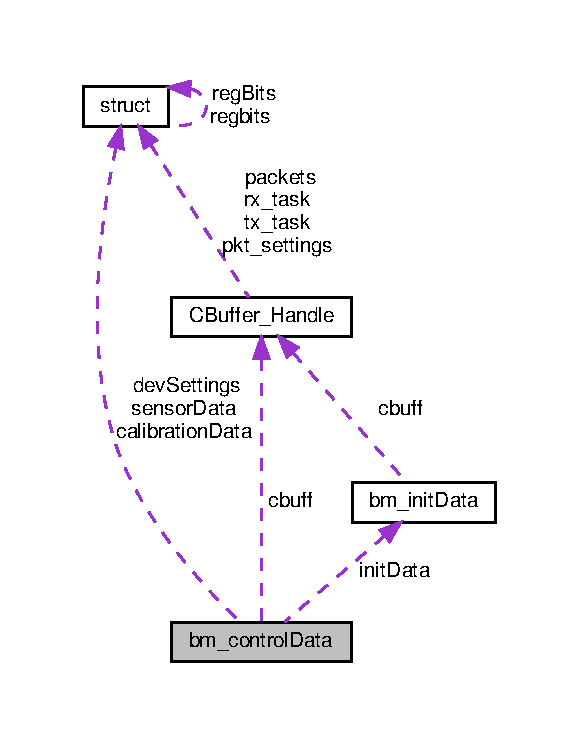
\includegraphics[width=278pt]{structbm__controlData__coll__graph}
\end{center}
\end{figure}
\subsection*{Public Attributes}
\begin{DoxyCompactItemize}
\item 
\hyperlink{structBM__CalibrationData}{bm\+\_\+calibration\+Data\+\_\+t} \hyperlink{structbm__controlData_ac4a27ff2241323607245cbcb92f116f1}{calibration\+Data}
\item 
\hyperlink{structBM__sensorData}{bm\+\_\+sensor\+Data\+\_\+t} \hyperlink{structbm__controlData_a193dc45579d41ddf5273944cc8e0280c}{sensor\+Data}
\item 
\hyperlink{structbm__deviceSettings}{bm\+\_\+device\+Settings\+\_\+t} \hyperlink{structbm__controlData_af23dc8bec3148792f6fa2b437b6c4b7e}{dev\+Settings}
\item 
\hyperlink{structbm__initData}{bm\+\_\+init\+Data\+\_\+t} $\ast$ \hyperlink{structbm__controlData_a80c9c43ce6ae374806c612da04e03fd0}{init\+Data}
\item 
\hyperlink{vl53l0x__types_8h_aba7bc1797add20fe3efdf37ced1182c5}{uint8\+\_\+t} \hyperlink{structbm__controlData_a7364074fe9f7b59f28e97613070cc633}{peripheral\+ID}
\item 
\hyperlink{vl53l0x__types_8h_aba7bc1797add20fe3efdf37ced1182c5}{uint8\+\_\+t} \hyperlink{structbm__controlData_a22557e44c56d8291489a7e2d419bac88}{device\+Address}
\item 
\hyperlink{vl53l0x__types_8h_aba7bc1797add20fe3efdf37ced1182c5}{uint8\+\_\+t} \hyperlink{structbm__controlData_af40ad56e060f5584e4d4d31e3c3c48d8}{i2c\+Channel}
\item 
bool \hyperlink{structbm__controlData_a7309b6bd58f8c9fb1f5770f9eb1df3ee}{calibration\+Aquired}
\item 
\hyperlink{vl53l0x__types_8h_aba7bc1797add20fe3efdf37ced1182c5}{uint8\+\_\+t} \hyperlink{structbm__controlData_a895f3f4166087e92d8217c116f397bcf}{sample\+Mask}
\item 
\hyperlink{vl53l0x__types_8h_aba7bc1797add20fe3efdf37ced1182c5}{uint8\+\_\+t} \hyperlink{structbm__controlData_ae1f1f25c8af3e53abb7b98b6f109075e}{config\+Mask}
\item 
\mbox{\Hypertarget{structbm__controlData_aae381dd947ceca89878f4fa94896cc00}\label{structbm__controlData_aae381dd947ceca89878f4fa94896cc00}} 
bool {\bfseries use\+\_\+cbuffer}
\item 
\mbox{\Hypertarget{structbm__controlData_ab84eff19f4d1f3a54aa37d9533bbc70c}\label{structbm__controlData_ab84eff19f4d1f3a54aa37d9533bbc70c}} 
\hyperlink{structCBuffer__Handle}{C\+Buff} {\bfseries cbuff}
\end{DoxyCompactItemize}


\subsection{Member Data Documentation}
\mbox{\Hypertarget{structbm__controlData_a7309b6bd58f8c9fb1f5770f9eb1df3ee}\label{structbm__controlData_a7309b6bd58f8c9fb1f5770f9eb1df3ee}} 
\index{bm\+\_\+control\+Data@{bm\+\_\+control\+Data}!calibration\+Aquired@{calibration\+Aquired}}
\index{calibration\+Aquired@{calibration\+Aquired}!bm\+\_\+control\+Data@{bm\+\_\+control\+Data}}
\subsubsection{\texorpdfstring{calibration\+Aquired}{calibrationAquired}}
{\footnotesize\ttfamily bool bm\+\_\+control\+Data\+::calibration\+Aquired}

calibration data aquired \mbox{\Hypertarget{structbm__controlData_ac4a27ff2241323607245cbcb92f116f1}\label{structbm__controlData_ac4a27ff2241323607245cbcb92f116f1}} 
\index{bm\+\_\+control\+Data@{bm\+\_\+control\+Data}!calibration\+Data@{calibration\+Data}}
\index{calibration\+Data@{calibration\+Data}!bm\+\_\+control\+Data@{bm\+\_\+control\+Data}}
\subsubsection{\texorpdfstring{calibration\+Data}{calibrationData}}
{\footnotesize\ttfamily \hyperlink{structBM__CalibrationData}{bm\+\_\+calibration\+Data\+\_\+t} bm\+\_\+control\+Data\+::calibration\+Data}

the device calibrationdata \mbox{\Hypertarget{structbm__controlData_ae1f1f25c8af3e53abb7b98b6f109075e}\label{structbm__controlData_ae1f1f25c8af3e53abb7b98b6f109075e}} 
\index{bm\+\_\+control\+Data@{bm\+\_\+control\+Data}!config\+Mask@{config\+Mask}}
\index{config\+Mask@{config\+Mask}!bm\+\_\+control\+Data@{bm\+\_\+control\+Data}}
\subsubsection{\texorpdfstring{config\+Mask}{configMask}}
{\footnotesize\ttfamily \hyperlink{vl53l0x__types_8h_aba7bc1797add20fe3efdf37ced1182c5}{uint8\+\_\+t} bm\+\_\+control\+Data\+::config\+Mask}

config mask \mbox{\Hypertarget{structbm__controlData_a22557e44c56d8291489a7e2d419bac88}\label{structbm__controlData_a22557e44c56d8291489a7e2d419bac88}} 
\index{bm\+\_\+control\+Data@{bm\+\_\+control\+Data}!device\+Address@{device\+Address}}
\index{device\+Address@{device\+Address}!bm\+\_\+control\+Data@{bm\+\_\+control\+Data}}
\subsubsection{\texorpdfstring{device\+Address}{deviceAddress}}
{\footnotesize\ttfamily \hyperlink{vl53l0x__types_8h_aba7bc1797add20fe3efdf37ced1182c5}{uint8\+\_\+t} bm\+\_\+control\+Data\+::device\+Address}

the device\textquotesingle{}s I2C address \mbox{\Hypertarget{structbm__controlData_af23dc8bec3148792f6fa2b437b6c4b7e}\label{structbm__controlData_af23dc8bec3148792f6fa2b437b6c4b7e}} 
\index{bm\+\_\+control\+Data@{bm\+\_\+control\+Data}!dev\+Settings@{dev\+Settings}}
\index{dev\+Settings@{dev\+Settings}!bm\+\_\+control\+Data@{bm\+\_\+control\+Data}}
\subsubsection{\texorpdfstring{dev\+Settings}{devSettings}}
{\footnotesize\ttfamily \hyperlink{structbm__deviceSettings}{bm\+\_\+device\+Settings\+\_\+t} bm\+\_\+control\+Data\+::dev\+Settings}

the device settings \mbox{\Hypertarget{structbm__controlData_af40ad56e060f5584e4d4d31e3c3c48d8}\label{structbm__controlData_af40ad56e060f5584e4d4d31e3c3c48d8}} 
\index{bm\+\_\+control\+Data@{bm\+\_\+control\+Data}!i2c\+Channel@{i2c\+Channel}}
\index{i2c\+Channel@{i2c\+Channel}!bm\+\_\+control\+Data@{bm\+\_\+control\+Data}}
\subsubsection{\texorpdfstring{i2c\+Channel}{i2cChannel}}
{\footnotesize\ttfamily \hyperlink{vl53l0x__types_8h_aba7bc1797add20fe3efdf37ced1182c5}{uint8\+\_\+t} bm\+\_\+control\+Data\+::i2c\+Channel}

the i2c channel used \mbox{\Hypertarget{structbm__controlData_a80c9c43ce6ae374806c612da04e03fd0}\label{structbm__controlData_a80c9c43ce6ae374806c612da04e03fd0}} 
\index{bm\+\_\+control\+Data@{bm\+\_\+control\+Data}!init\+Data@{init\+Data}}
\index{init\+Data@{init\+Data}!bm\+\_\+control\+Data@{bm\+\_\+control\+Data}}
\subsubsection{\texorpdfstring{init\+Data}{initData}}
{\footnotesize\ttfamily \hyperlink{structbm__initData}{bm\+\_\+init\+Data\+\_\+t}$\ast$ bm\+\_\+control\+Data\+::init\+Data}

pointer to the init data \mbox{\Hypertarget{structbm__controlData_a7364074fe9f7b59f28e97613070cc633}\label{structbm__controlData_a7364074fe9f7b59f28e97613070cc633}} 
\index{bm\+\_\+control\+Data@{bm\+\_\+control\+Data}!peripheral\+ID@{peripheral\+ID}}
\index{peripheral\+ID@{peripheral\+ID}!bm\+\_\+control\+Data@{bm\+\_\+control\+Data}}
\subsubsection{\texorpdfstring{peripheral\+ID}{peripheralID}}
{\footnotesize\ttfamily \hyperlink{vl53l0x__types_8h_aba7bc1797add20fe3efdf37ced1182c5}{uint8\+\_\+t} bm\+\_\+control\+Data\+::peripheral\+ID}

the periph\+\_\+id \mbox{\Hypertarget{structbm__controlData_a895f3f4166087e92d8217c116f397bcf}\label{structbm__controlData_a895f3f4166087e92d8217c116f397bcf}} 
\index{bm\+\_\+control\+Data@{bm\+\_\+control\+Data}!sample\+Mask@{sample\+Mask}}
\index{sample\+Mask@{sample\+Mask}!bm\+\_\+control\+Data@{bm\+\_\+control\+Data}}
\subsubsection{\texorpdfstring{sample\+Mask}{sampleMask}}
{\footnotesize\ttfamily \hyperlink{vl53l0x__types_8h_aba7bc1797add20fe3efdf37ced1182c5}{uint8\+\_\+t} bm\+\_\+control\+Data\+::sample\+Mask}

sample mask \mbox{\Hypertarget{structbm__controlData_a193dc45579d41ddf5273944cc8e0280c}\label{structbm__controlData_a193dc45579d41ddf5273944cc8e0280c}} 
\index{bm\+\_\+control\+Data@{bm\+\_\+control\+Data}!sensor\+Data@{sensor\+Data}}
\index{sensor\+Data@{sensor\+Data}!bm\+\_\+control\+Data@{bm\+\_\+control\+Data}}
\subsubsection{\texorpdfstring{sensor\+Data}{sensorData}}
{\footnotesize\ttfamily \hyperlink{structBM__sensorData}{bm\+\_\+sensor\+Data\+\_\+t} bm\+\_\+control\+Data\+::sensor\+Data}

the device sensor data 

The documentation for this struct was generated from the following file\+:\begin{DoxyCompactItemize}
\item 
B\+M\+E280\+\_\+\+Driver/B\+M\+E280\+\_\+\+Driver.\+h\end{DoxyCompactItemize}

\hypertarget{structbm__deviceSettings}{}\section{bm\+\_\+device\+Settings Struct Reference}
\label{structbm__deviceSettings}\index{bm\+\_\+device\+Settings@{bm\+\_\+device\+Settings}}
\subsection*{Public Attributes}
\begin{DoxyCompactItemize}
\item 
\mbox{\Hypertarget{structbm__deviceSettings_a6fe879b166151f3bfaf5a0ac1f7962ea}\label{structbm__deviceSettings_a6fe879b166151f3bfaf5a0ac1f7962ea}} 
bm\+\_\+sample\+Type\+\_\+t {\bfseries sample\+Type}
\item 
\mbox{\Hypertarget{structbm__deviceSettings_abac93a0a0d1369273da8b0937b29d4c1}\label{structbm__deviceSettings_abac93a0a0d1369273da8b0937b29d4c1}} 
B\+M\+\_\+sample\+Mode\+\_\+t {\bfseries sample\+Mode}
\item 
\mbox{\Hypertarget{structbm__deviceSettings_ad1c4a858d81d9364d72c6ac59c4eccfa}\label{structbm__deviceSettings_ad1c4a858d81d9364d72c6ac59c4eccfa}} 
B\+M\+\_\+over\+Sample\+\_\+t {\bfseries temp\+OS}
\item 
\mbox{\Hypertarget{structbm__deviceSettings_a68dd199eb5397c72a799a000e219ed36}\label{structbm__deviceSettings_a68dd199eb5397c72a799a000e219ed36}} 
B\+M\+\_\+over\+Sample\+\_\+t {\bfseries press\+OS}
\item 
\mbox{\Hypertarget{structbm__deviceSettings_a0540c69071e9c8fec6a7bbb1d8091e43}\label{structbm__deviceSettings_a0540c69071e9c8fec6a7bbb1d8091e43}} 
B\+M\+\_\+over\+Sample\+\_\+t {\bfseries humid\+OS}
\item 
\mbox{\Hypertarget{structbm__deviceSettings_a9e7e56f90ad7e6b2eaad04d58f48400b}\label{structbm__deviceSettings_a9e7e56f90ad7e6b2eaad04d58f48400b}} 
B\+M\+\_\+standby\+T\+\_\+t {\bfseries sample\+Interval}
\item 
\mbox{\Hypertarget{structbm__deviceSettings_ae8c554fada240f44f28b4850848c42db}\label{structbm__deviceSettings_ae8c554fada240f44f28b4850848c42db}} 
bm\+\_\+filter\+\_\+t {\bfseries filter\+Coefficient}
\end{DoxyCompactItemize}


The documentation for this struct was generated from the following file\+:\begin{DoxyCompactItemize}
\item 
B\+M\+E280\+\_\+\+Driver/B\+M\+E280\+\_\+\+Driver.\+h\end{DoxyCompactItemize}

\hypertarget{structbm__initData}{}\section{bm\+\_\+init\+Data Struct Reference}
\label{structbm__initData}\index{bm\+\_\+init\+Data@{bm\+\_\+init\+Data}}


Collaboration diagram for bm\+\_\+init\+Data\+:\nopagebreak
\begin{figure}[H]
\begin{center}
\leavevmode
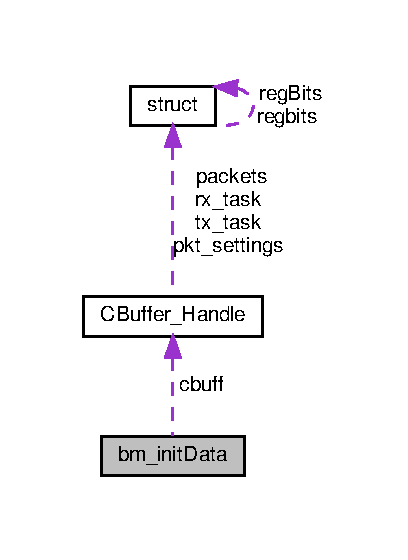
\includegraphics[width=196pt]{structbm__initData__coll__graph}
\end{center}
\end{figure}
\subsection*{Public Attributes}
\begin{DoxyCompactItemize}
\item 
\mbox{\Hypertarget{structbm__initData_a190573a231e043683f5d56706f83c57f}\label{structbm__initData_a190573a231e043683f5d56706f83c57f}} 
B\+M\+\_\+device\+Type\+\_\+t {\bfseries dev\+Type}
\item 
\mbox{\Hypertarget{structbm__initData_aa57e27b3a27b573a068ab2aff0a5eda9}\label{structbm__initData_aa57e27b3a27b573a068ab2aff0a5eda9}} 
bm\+\_\+sample\+Type\+\_\+t {\bfseries sample\+Type}
\item 
\mbox{\Hypertarget{structbm__initData_a6fba51e1a283f9906a9ba726a5c72c5f}\label{structbm__initData_a6fba51e1a283f9906a9ba726a5c72c5f}} 
B\+M\+\_\+sample\+Mode\+\_\+t {\bfseries sample\+Mode}
\item 
\mbox{\Hypertarget{structbm__initData_a7f827d76e1cd9d466ebf7808637f9802}\label{structbm__initData_a7f827d76e1cd9d466ebf7808637f9802}} 
bool {\bfseries address\+Pin\+State}
\item 
\mbox{\Hypertarget{structbm__initData_a3c93ebe9567281b7b6d3a206a568f1fe}\label{structbm__initData_a3c93ebe9567281b7b6d3a206a568f1fe}} 
\hyperlink{vl53l0x__types_8h_aba7bc1797add20fe3efdf37ced1182c5}{uint8\+\_\+t} {\bfseries i2c\+Channel}
\item 
bool \hyperlink{structbm__initData_a147cdbe81bcbd04fd35e560d84438481}{use\+\_\+cbuffer}
\item 
\mbox{\Hypertarget{structbm__initData_a1db9fa0fbd20d6e568a981c08b4c5750}\label{structbm__initData_a1db9fa0fbd20d6e568a981c08b4c5750}} 
\hyperlink{structCBuffer__Handle}{C\+Buff} {\bfseries cbuff}
\end{DoxyCompactItemize}


\subsection{Member Data Documentation}
\mbox{\Hypertarget{structbm__initData_a147cdbe81bcbd04fd35e560d84438481}\label{structbm__initData_a147cdbe81bcbd04fd35e560d84438481}} 
\index{bm\+\_\+init\+Data@{bm\+\_\+init\+Data}!use\+\_\+cbuffer@{use\+\_\+cbuffer}}
\index{use\+\_\+cbuffer@{use\+\_\+cbuffer}!bm\+\_\+init\+Data@{bm\+\_\+init\+Data}}
\subsubsection{\texorpdfstring{use\+\_\+cbuffer}{use\_cbuffer}}
{\footnotesize\ttfamily bool bm\+\_\+init\+Data\+::use\+\_\+cbuffer}

$<$ 0 -\/ no i2c initialised, driver will init. 1 $\vert$ 2, valid i2c channels 

The documentation for this struct was generated from the following file\+:\begin{DoxyCompactItemize}
\item 
B\+M\+E280\+\_\+\+Driver/B\+M\+E280\+\_\+\+Driver.\+h\end{DoxyCompactItemize}

\hypertarget{structBM__sensorData}{}\section{B\+M\+\_\+sensor\+Data Struct Reference}
\label{structBM__sensorData}\index{B\+M\+\_\+sensor\+Data@{B\+M\+\_\+sensor\+Data}}
\subsection*{Public Attributes}
\begin{DoxyCompactItemize}
\item 
\mbox{\Hypertarget{structBM__sensorData_ab277f2f8b5738386bd951ac2fd30bd28}\label{structBM__sensorData_ab277f2f8b5738386bd951ac2fd30bd28}} 
float {\bfseries real\+Temperature}
\item 
\hyperlink{vl53l0x__types_8h_a435d1572bf3f880d55459d9805097f62}{uint32\+\_\+t} \hyperlink{structBM__sensorData_a3ab64fd19caf636950cb47ca2697cd6f}{calibrated\+Temperature}
\item 
\hyperlink{vl53l0x__types_8h_a435d1572bf3f880d55459d9805097f62}{uint32\+\_\+t} \hyperlink{structBM__sensorData_a59c55713af263f1533b9b2481f2af860}{raw\+Temperature}
\item 
float \hyperlink{structBM__sensorData_a616031c2e11814b054f9f43e7fce12fc}{real\+Pressure}
\item 
\hyperlink{vl53l0x__types_8h_a435d1572bf3f880d55459d9805097f62}{uint32\+\_\+t} \hyperlink{structBM__sensorData_ae28102363bbe4c8567103f3f7bc4799f}{calibrated\+Pressure}
\item 
\hyperlink{vl53l0x__types_8h_a435d1572bf3f880d55459d9805097f62}{uint32\+\_\+t} \hyperlink{structBM__sensorData_a1f2b1f5547b72be0682ea296ba63144c}{raw\+Pressure}
\item 
float \hyperlink{structBM__sensorData_ab1aac1511aef5fe07ecddf763329c038}{real\+Humidity}
\item 
\hyperlink{vl53l0x__types_8h_a435d1572bf3f880d55459d9805097f62}{uint32\+\_\+t} \hyperlink{structBM__sensorData_a0a220c8916aedd66c95e44548ec33e0f}{calibrated\+Humidity}
\item 
\hyperlink{vl53l0x__types_8h_a435d1572bf3f880d55459d9805097f62}{uint32\+\_\+t} \hyperlink{structBM__sensorData_a017dd76d7efffc01ecfe7d7bac5fdc7f}{raw\+Humidity}
\item 
\hyperlink{vl53l0x__types_8h_aba7bc1797add20fe3efdf37ced1182c5}{uint8\+\_\+t} \hyperlink{structBM__sensorData_ac415745c07825ddb08643ef66c2ec1a9}{status\+Measure}
\item 
\mbox{\Hypertarget{structBM__sensorData_abe0b6e503d1458e83510a6dba728137e}\label{structBM__sensorData_abe0b6e503d1458e83510a6dba728137e}} 
\hyperlink{vl53l0x__types_8h_aba7bc1797add20fe3efdf37ced1182c5}{uint8\+\_\+t} {\bfseries status\+Update}
\end{DoxyCompactItemize}


\subsection{Member Data Documentation}
\mbox{\Hypertarget{structBM__sensorData_a0a220c8916aedd66c95e44548ec33e0f}\label{structBM__sensorData_a0a220c8916aedd66c95e44548ec33e0f}} 
\index{B\+M\+\_\+sensor\+Data@{B\+M\+\_\+sensor\+Data}!calibrated\+Humidity@{calibrated\+Humidity}}
\index{calibrated\+Humidity@{calibrated\+Humidity}!B\+M\+\_\+sensor\+Data@{B\+M\+\_\+sensor\+Data}}
\subsubsection{\texorpdfstring{calibrated\+Humidity}{calibratedHumidity}}
{\footnotesize\ttfamily \hyperlink{vl53l0x__types_8h_a435d1572bf3f880d55459d9805097f62}{uint32\+\_\+t} B\+M\+\_\+sensor\+Data\+::calibrated\+Humidity}

$<$ real humidity in RH \mbox{\Hypertarget{structBM__sensorData_ae28102363bbe4c8567103f3f7bc4799f}\label{structBM__sensorData_ae28102363bbe4c8567103f3f7bc4799f}} 
\index{B\+M\+\_\+sensor\+Data@{B\+M\+\_\+sensor\+Data}!calibrated\+Pressure@{calibrated\+Pressure}}
\index{calibrated\+Pressure@{calibrated\+Pressure}!B\+M\+\_\+sensor\+Data@{B\+M\+\_\+sensor\+Data}}
\subsubsection{\texorpdfstring{calibrated\+Pressure}{calibratedPressure}}
{\footnotesize\ttfamily \hyperlink{vl53l0x__types_8h_a435d1572bf3f880d55459d9805097f62}{uint32\+\_\+t} B\+M\+\_\+sensor\+Data\+::calibrated\+Pressure}

$<$ real pressure in h\+Pa \mbox{\Hypertarget{structBM__sensorData_a3ab64fd19caf636950cb47ca2697cd6f}\label{structBM__sensorData_a3ab64fd19caf636950cb47ca2697cd6f}} 
\index{B\+M\+\_\+sensor\+Data@{B\+M\+\_\+sensor\+Data}!calibrated\+Temperature@{calibrated\+Temperature}}
\index{calibrated\+Temperature@{calibrated\+Temperature}!B\+M\+\_\+sensor\+Data@{B\+M\+\_\+sensor\+Data}}
\subsubsection{\texorpdfstring{calibrated\+Temperature}{calibratedTemperature}}
{\footnotesize\ttfamily \hyperlink{vl53l0x__types_8h_a435d1572bf3f880d55459d9805097f62}{uint32\+\_\+t} B\+M\+\_\+sensor\+Data\+::calibrated\+Temperature}

$<$ real temperature in degrees C \mbox{\Hypertarget{structBM__sensorData_a017dd76d7efffc01ecfe7d7bac5fdc7f}\label{structBM__sensorData_a017dd76d7efffc01ecfe7d7bac5fdc7f}} 
\index{B\+M\+\_\+sensor\+Data@{B\+M\+\_\+sensor\+Data}!raw\+Humidity@{raw\+Humidity}}
\index{raw\+Humidity@{raw\+Humidity}!B\+M\+\_\+sensor\+Data@{B\+M\+\_\+sensor\+Data}}
\subsubsection{\texorpdfstring{raw\+Humidity}{rawHumidity}}
{\footnotesize\ttfamily \hyperlink{vl53l0x__types_8h_a435d1572bf3f880d55459d9805097f62}{uint32\+\_\+t} B\+M\+\_\+sensor\+Data\+::raw\+Humidity}

$<$ \char`\"{}    \char`\"{} \char`\"{}    \char`\"{} humidity calibration \mbox{\Hypertarget{structBM__sensorData_a1f2b1f5547b72be0682ea296ba63144c}\label{structBM__sensorData_a1f2b1f5547b72be0682ea296ba63144c}} 
\index{B\+M\+\_\+sensor\+Data@{B\+M\+\_\+sensor\+Data}!raw\+Pressure@{raw\+Pressure}}
\index{raw\+Pressure@{raw\+Pressure}!B\+M\+\_\+sensor\+Data@{B\+M\+\_\+sensor\+Data}}
\subsubsection{\texorpdfstring{raw\+Pressure}{rawPressure}}
{\footnotesize\ttfamily \hyperlink{vl53l0x__types_8h_a435d1572bf3f880d55459d9805097f62}{uint32\+\_\+t} B\+M\+\_\+sensor\+Data\+::raw\+Pressure}

$<$ output of the pressure calibration \mbox{\Hypertarget{structBM__sensorData_a59c55713af263f1533b9b2481f2af860}\label{structBM__sensorData_a59c55713af263f1533b9b2481f2af860}} 
\index{B\+M\+\_\+sensor\+Data@{B\+M\+\_\+sensor\+Data}!raw\+Temperature@{raw\+Temperature}}
\index{raw\+Temperature@{raw\+Temperature}!B\+M\+\_\+sensor\+Data@{B\+M\+\_\+sensor\+Data}}
\subsubsection{\texorpdfstring{raw\+Temperature}{rawTemperature}}
{\footnotesize\ttfamily \hyperlink{vl53l0x__types_8h_a435d1572bf3f880d55459d9805097f62}{uint32\+\_\+t} B\+M\+\_\+sensor\+Data\+::raw\+Temperature}

$<$ output of the temp calibration \mbox{\Hypertarget{structBM__sensorData_ab1aac1511aef5fe07ecddf763329c038}\label{structBM__sensorData_ab1aac1511aef5fe07ecddf763329c038}} 
\index{B\+M\+\_\+sensor\+Data@{B\+M\+\_\+sensor\+Data}!real\+Humidity@{real\+Humidity}}
\index{real\+Humidity@{real\+Humidity}!B\+M\+\_\+sensor\+Data@{B\+M\+\_\+sensor\+Data}}
\subsubsection{\texorpdfstring{real\+Humidity}{realHumidity}}
{\footnotesize\ttfamily float B\+M\+\_\+sensor\+Data\+::real\+Humidity}

$<$ output of the device register \mbox{\Hypertarget{structBM__sensorData_a616031c2e11814b054f9f43e7fce12fc}\label{structBM__sensorData_a616031c2e11814b054f9f43e7fce12fc}} 
\index{B\+M\+\_\+sensor\+Data@{B\+M\+\_\+sensor\+Data}!real\+Pressure@{real\+Pressure}}
\index{real\+Pressure@{real\+Pressure}!B\+M\+\_\+sensor\+Data@{B\+M\+\_\+sensor\+Data}}
\subsubsection{\texorpdfstring{real\+Pressure}{realPressure}}
{\footnotesize\ttfamily float B\+M\+\_\+sensor\+Data\+::real\+Pressure}

$<$ output of the device register \mbox{\Hypertarget{structBM__sensorData_ac415745c07825ddb08643ef66c2ec1a9}\label{structBM__sensorData_ac415745c07825ddb08643ef66c2ec1a9}} 
\index{B\+M\+\_\+sensor\+Data@{B\+M\+\_\+sensor\+Data}!status\+Measure@{status\+Measure}}
\index{status\+Measure@{status\+Measure}!B\+M\+\_\+sensor\+Data@{B\+M\+\_\+sensor\+Data}}
\subsubsection{\texorpdfstring{status\+Measure}{statusMeasure}}
{\footnotesize\ttfamily \hyperlink{vl53l0x__types_8h_aba7bc1797add20fe3efdf37ced1182c5}{uint8\+\_\+t} B\+M\+\_\+sensor\+Data\+::status\+Measure}

$<$ output of the device register 

The documentation for this struct was generated from the following file\+:\begin{DoxyCompactItemize}
\item 
B\+M\+E280\+\_\+\+Driver/B\+M\+E280\+\_\+\+Driver.\+h\end{DoxyCompactItemize}

\hypertarget{structbuttonData}{}\section{button\+Data Struct Reference}
\label{structbuttonData}\index{button\+Data@{button\+Data}}
\subsection*{Public Attributes}
\begin{DoxyCompactItemize}
\item 
\mbox{\Hypertarget{structbuttonData_abda9de5ae492f575ac826531b6c13249}\label{structbuttonData_abda9de5ae492f575ac826531b6c13249}} 
bool {\bfseries btn\+Debounce\+Enable}
\item 
bool \hyperlink{structbuttonData_afa9608155098295140e8fbae290c162c}{btn\+Debounce\+State}
\item 
bool \hyperlink{structbuttonData_a738bdc48430aa378eb278a8759cfcd0f}{btn\+State}
\item 
bool \hyperlink{structbuttonData_a4a60f7d8d5649d2470790f43244c8a3f}{alert\+Btn}
\item 
bool \hyperlink{structbuttonData_a04bf36fc0adf605c9f7352ab41af134c}{half\+Btn\+Interrupt}
\item 
btn\+\_\+config\+\_\+t \hyperlink{structbuttonData_a77b4789cd0f59ad4238149317efa20c0}{btn\+\_\+setting}
\item 
\mbox{\Hypertarget{structbuttonData_a28871f000e0e6eeca11fb5bcf48cbe9c}\label{structbuttonData_a28871f000e0e6eeca11fb5bcf48cbe9c}} 
\hyperlink{vl53l0x__types_8h_a273cf69d639a59973b6019625df33e30}{uint16\+\_\+t} {\bfseries btn\+Count}
\item 
\hyperlink{vl53l0x__types_8h_a435d1572bf3f880d55459d9805097f62}{uint32\+\_\+t} \hyperlink{structbuttonData_ad8db5fdf61df4a87f43d487cc35d65bf}{t\+Last\+Btn}
\item 
\hyperlink{vl53l0x__types_8h_a435d1572bf3f880d55459d9805097f62}{uint32\+\_\+t} \hyperlink{structbuttonData_a325b9db7bb86ad831153318656891a8b}{t\+Btn\+Press}
\item 
\hyperlink{vl53l0x__types_8h_a273cf69d639a59973b6019625df33e30}{uint16\+\_\+t} \hyperlink{structbuttonData_a172467069638e0427e606e58408f25b3}{t\+Debounce}
\item 
esp\+\_\+event\+\_\+loop\+\_\+handle\+\_\+t \hyperlink{structbuttonData_a78456e82e30bcce95328039367be38dd}{loop}
\item 
\mbox{\Hypertarget{structbuttonData_af98a75d1042dbd7254f92846ff4e572f}\label{structbuttonData_af98a75d1042dbd7254f92846ff4e572f}} 
Timer\+Handle\+\_\+t {\bfseries debounce\+Timer}
\item 
Task\+Handle\+\_\+t \hyperlink{structbuttonData_a9ab9462764966d50b44f0b8cfc0dd202}{parent\+Task}
\item 
gpio\+\_\+num\+\_\+t \hyperlink{structbuttonData_a22a4c876c877761e6380b7712e86db3b}{btn\+Pin}
\end{DoxyCompactItemize}


\subsection{Member Data Documentation}
\mbox{\Hypertarget{structbuttonData_a4a60f7d8d5649d2470790f43244c8a3f}\label{structbuttonData_a4a60f7d8d5649d2470790f43244c8a3f}} 
\index{button\+Data@{button\+Data}!alert\+Btn@{alert\+Btn}}
\index{alert\+Btn@{alert\+Btn}!button\+Data@{button\+Data}}
\subsubsection{\texorpdfstring{alert\+Btn}{alertBtn}}
{\footnotesize\ttfamily bool button\+Data\+::alert\+Btn}

$<$ bool btn\+State\+: current state of button (ie pin state) \mbox{\Hypertarget{structbuttonData_a77b4789cd0f59ad4238149317efa20c0}\label{structbuttonData_a77b4789cd0f59ad4238149317efa20c0}} 
\index{button\+Data@{button\+Data}!btn\+\_\+setting@{btn\+\_\+setting}}
\index{btn\+\_\+setting@{btn\+\_\+setting}!button\+Data@{button\+Data}}
\subsubsection{\texorpdfstring{btn\+\_\+setting}{btn\_setting}}
{\footnotesize\ttfamily btn\+\_\+config\+\_\+t button\+Data\+::btn\+\_\+setting}

$<$ send the notify on each edge change, rather than whole button cycle \mbox{\Hypertarget{structbuttonData_afa9608155098295140e8fbae290c162c}\label{structbuttonData_afa9608155098295140e8fbae290c162c}} 
\index{button\+Data@{button\+Data}!btn\+Debounce\+State@{btn\+Debounce\+State}}
\index{btn\+Debounce\+State@{btn\+Debounce\+State}!button\+Data@{button\+Data}}
\subsubsection{\texorpdfstring{btn\+Debounce\+State}{btnDebounceState}}
{\footnotesize\ttfamily bool button\+Data\+::btn\+Debounce\+State}

$<$ bool btn\+Debounce\+Enable\+: enable to button debounce \mbox{\Hypertarget{structbuttonData_a22a4c876c877761e6380b7712e86db3b}\label{structbuttonData_a22a4c876c877761e6380b7712e86db3b}} 
\index{button\+Data@{button\+Data}!btn\+Pin@{btn\+Pin}}
\index{btn\+Pin@{btn\+Pin}!button\+Data@{button\+Data}}
\subsubsection{\texorpdfstring{btn\+Pin}{btnPin}}
{\footnotesize\ttfamily gpio\+\_\+num\+\_\+t button\+Data\+::btn\+Pin}

$<$ Task to notify \mbox{\Hypertarget{structbuttonData_a738bdc48430aa378eb278a8759cfcd0f}\label{structbuttonData_a738bdc48430aa378eb278a8759cfcd0f}} 
\index{button\+Data@{button\+Data}!btn\+State@{btn\+State}}
\index{btn\+State@{btn\+State}!button\+Data@{button\+Data}}
\subsubsection{\texorpdfstring{btn\+State}{btnState}}
{\footnotesize\ttfamily bool button\+Data\+::btn\+State}

$<$ bool btn\+Debounce\+State\+: button debounce state \mbox{\Hypertarget{structbuttonData_a04bf36fc0adf605c9f7352ab41af134c}\label{structbuttonData_a04bf36fc0adf605c9f7352ab41af134c}} 
\index{button\+Data@{button\+Data}!half\+Btn\+Interrupt@{half\+Btn\+Interrupt}}
\index{half\+Btn\+Interrupt@{half\+Btn\+Interrupt}!button\+Data@{button\+Data}}
\subsubsection{\texorpdfstring{half\+Btn\+Interrupt}{halfBtnInterrupt}}
{\footnotesize\ttfamily bool button\+Data\+::half\+Btn\+Interrupt}

$<$ bool alert\+Btn\+: send task notification if button pressed -\/ default on with parent\+Task \mbox{\Hypertarget{structbuttonData_a78456e82e30bcce95328039367be38dd}\label{structbuttonData_a78456e82e30bcce95328039367be38dd}} 
\index{button\+Data@{button\+Data}!loop@{loop}}
\index{loop@{loop}!button\+Data@{button\+Data}}
\subsubsection{\texorpdfstring{loop}{loop}}
{\footnotesize\ttfamily esp\+\_\+event\+\_\+loop\+\_\+handle\+\_\+t button\+Data\+::loop}

$<$ length of DB timer cooldown in ms \mbox{\Hypertarget{structbuttonData_a9ab9462764966d50b44f0b8cfc0dd202}\label{structbuttonData_a9ab9462764966d50b44f0b8cfc0dd202}} 
\index{button\+Data@{button\+Data}!parent\+Task@{parent\+Task}}
\index{parent\+Task@{parent\+Task}!button\+Data@{button\+Data}}
\subsubsection{\texorpdfstring{parent\+Task}{parentTask}}
{\footnotesize\ttfamily Task\+Handle\+\_\+t button\+Data\+::parent\+Task}

$<$ Timer for debounce \mbox{\Hypertarget{structbuttonData_a325b9db7bb86ad831153318656891a8b}\label{structbuttonData_a325b9db7bb86ad831153318656891a8b}} 
\index{button\+Data@{button\+Data}!t\+Btn\+Press@{t\+Btn\+Press}}
\index{t\+Btn\+Press@{t\+Btn\+Press}!button\+Data@{button\+Data}}
\subsubsection{\texorpdfstring{t\+Btn\+Press}{tBtnPress}}
{\footnotesize\ttfamily \hyperlink{vl53l0x__types_8h_a435d1572bf3f880d55459d9805097f62}{uint32\+\_\+t} button\+Data\+::t\+Btn\+Press}

$<$ time since last button push \mbox{\Hypertarget{structbuttonData_a172467069638e0427e606e58408f25b3}\label{structbuttonData_a172467069638e0427e606e58408f25b3}} 
\index{button\+Data@{button\+Data}!t\+Debounce@{t\+Debounce}}
\index{t\+Debounce@{t\+Debounce}!button\+Data@{button\+Data}}
\subsubsection{\texorpdfstring{t\+Debounce}{tDebounce}}
{\footnotesize\ttfamily \hyperlink{vl53l0x__types_8h_a273cf69d639a59973b6019625df33e30}{uint16\+\_\+t} button\+Data\+::t\+Debounce}

$<$ time the button is held down for \mbox{\Hypertarget{structbuttonData_ad8db5fdf61df4a87f43d487cc35d65bf}\label{structbuttonData_ad8db5fdf61df4a87f43d487cc35d65bf}} 
\index{button\+Data@{button\+Data}!t\+Last\+Btn@{t\+Last\+Btn}}
\index{t\+Last\+Btn@{t\+Last\+Btn}!button\+Data@{button\+Data}}
\subsubsection{\texorpdfstring{t\+Last\+Btn}{tLastBtn}}
{\footnotesize\ttfamily \hyperlink{vl53l0x__types_8h_a435d1572bf3f880d55459d9805097f62}{uint32\+\_\+t} button\+Data\+::t\+Last\+Btn}

$<$ number of button pushes 

The documentation for this struct was generated from the following file\+:\begin{DoxyCompactItemize}
\item 
Pushbutton\+\_\+\+Driver/Push\+Button\+\_\+\+Driver.\+h\end{DoxyCompactItemize}

\hypertarget{structCBuffer__Handle}{}\section{C\+Buffer\+\_\+\+Handle Struct Reference}
\label{structCBuffer__Handle}\index{C\+Buffer\+\_\+\+Handle@{C\+Buffer\+\_\+\+Handle}}


{\ttfamily \#include $<$Circular\+Buffer.\+h$>$}



Collaboration diagram for C\+Buffer\+\_\+\+Handle\+:\nopagebreak
\begin{figure}[H]
\begin{center}
\leavevmode
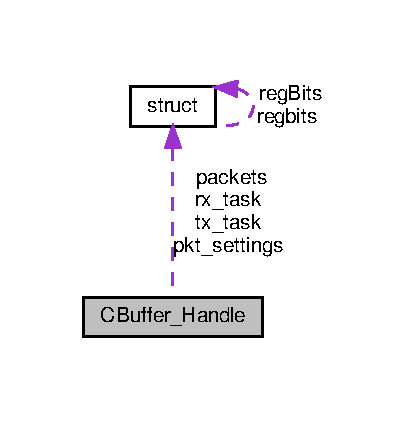
\includegraphics[width=196pt]{structCBuffer__Handle__coll__graph}
\end{center}
\end{figure}
\subsection*{Public Attributes}
\begin{DoxyCompactItemize}
\item 
void $\ast$ \hyperlink{structCBuffer__Handle_ace9001395e4926b7da1c5ec82afd20b3}{buffer\+\_\+start}
\item 
void $\ast$ \hyperlink{structCBuffer__Handle_aa8573cb52319451c021516d1a906c970}{buffer\+\_\+end}
\item 
void $\ast$ \hyperlink{structCBuffer__Handle_a3e996c49d0c489498b43d16ff1df810b}{read\+\_\+ptr}
\item 
void $\ast$ \hyperlink{structCBuffer__Handle_a301255119721b1cc76531ffc045594fb}{write\+\_\+ptr}
\item 
\hyperlink{vl53l0x__types_8h_a435d1572bf3f880d55459d9805097f62}{uint32\+\_\+t} \hyperlink{structCBuffer__Handle_af0549758ada54a9e9117a0c4ff0a4955}{buffer\+\_\+len}
\item 
\hyperlink{vl53l0x__types_8h_a273cf69d639a59973b6019625df33e30}{uint16\+\_\+t} \hyperlink{structCBuffer__Handle_aed2d7a4a93b8f607d51b93300c5837b5}{data\+\_\+len}
\item 
bool \hyperlink{structCBuffer__Handle_a1a41fc5596188b457815ca1c5afafccd}{allow\+\_\+overwrite}
\item 
bool \hyperlink{structCBuffer__Handle_a7019a6c91cfbcc0e02e11b8895450cc6}{is\+\_\+claimed}
\item 
bool \hyperlink{structCBuffer__Handle_ad6156a0a6134052e1620d8cd9fb5154b}{use\+\_\+packets}
\item 
\hyperlink{structCBuffer__packet__member}{cbuffer\+\_\+pmember\+\_\+t} \hyperlink{structCBuffer__Handle_ad2465a41c6b7bf39ea5a11d47836e841}{packets} \mbox{[}C\+B\+U\+F\+F\+E\+R\+\_\+\+M\+A\+X\+\_\+\+P\+A\+C\+K\+E\+T\+\_\+\+V\+A\+L\+U\+ES\mbox{]}
\item 
\hyperlink{structcbuffer__packet__settings}{cbuffer\+\_\+pkt\+\_\+settings\+\_\+t} \hyperlink{structCBuffer__Handle_aa8610091db61fb607b93b5374b076307}{pkt\+\_\+settings}
\item 
\hyperlink{vl53l0x__types_8h_a273cf69d639a59973b6019625df33e30}{uint16\+\_\+t} \hyperlink{structCBuffer__Handle_a54e07db8fad941c1ec2b5eadbeeeb16e}{pkts\+\_\+available}
\item 
Semaphore\+Handle\+\_\+t \hyperlink{structCBuffer__Handle_a3774a4f2a54b9cd40367b87ee52c5e69}{sem}
\item 
\hyperlink{structCBuffer__tasks}{cbuffer\+\_\+task\+\_\+settings\+\_\+t} \hyperlink{structCBuffer__Handle_acf4f92865eae15d0c64e94550bb0ac9a}{tx\+\_\+task}
\item 
\mbox{\Hypertarget{structCBuffer__Handle_ad57ecec79ac6e597d9bc5d093ed26cc5}\label{structCBuffer__Handle_ad57ecec79ac6e597d9bc5d093ed26cc5}} 
\hyperlink{structCBuffer__tasks}{cbuffer\+\_\+task\+\_\+settings\+\_\+t} {\bfseries rx\+\_\+task}
\end{DoxyCompactItemize}


\subsection{Detailed Description}
the cbuffer handle data structure 

\subsection{Member Data Documentation}
\mbox{\Hypertarget{structCBuffer__Handle_a1a41fc5596188b457815ca1c5afafccd}\label{structCBuffer__Handle_a1a41fc5596188b457815ca1c5afafccd}} 
\index{C\+Buffer\+\_\+\+Handle@{C\+Buffer\+\_\+\+Handle}!allow\+\_\+overwrite@{allow\+\_\+overwrite}}
\index{allow\+\_\+overwrite@{allow\+\_\+overwrite}!C\+Buffer\+\_\+\+Handle@{C\+Buffer\+\_\+\+Handle}}
\subsubsection{\texorpdfstring{allow\+\_\+overwrite}{allow\_overwrite}}
{\footnotesize\ttfamily bool C\+Buffer\+\_\+\+Handle\+::allow\+\_\+overwrite}

allow overwrite of unread data \mbox{\Hypertarget{structCBuffer__Handle_aa8573cb52319451c021516d1a906c970}\label{structCBuffer__Handle_aa8573cb52319451c021516d1a906c970}} 
\index{C\+Buffer\+\_\+\+Handle@{C\+Buffer\+\_\+\+Handle}!buffer\+\_\+end@{buffer\+\_\+end}}
\index{buffer\+\_\+end@{buffer\+\_\+end}!C\+Buffer\+\_\+\+Handle@{C\+Buffer\+\_\+\+Handle}}
\subsubsection{\texorpdfstring{buffer\+\_\+end}{buffer\_end}}
{\footnotesize\ttfamily void$\ast$ C\+Buffer\+\_\+\+Handle\+::buffer\+\_\+end}

buffer end -\/ end of buffer addr \mbox{\Hypertarget{structCBuffer__Handle_af0549758ada54a9e9117a0c4ff0a4955}\label{structCBuffer__Handle_af0549758ada54a9e9117a0c4ff0a4955}} 
\index{C\+Buffer\+\_\+\+Handle@{C\+Buffer\+\_\+\+Handle}!buffer\+\_\+len@{buffer\+\_\+len}}
\index{buffer\+\_\+len@{buffer\+\_\+len}!C\+Buffer\+\_\+\+Handle@{C\+Buffer\+\_\+\+Handle}}
\subsubsection{\texorpdfstring{buffer\+\_\+len}{buffer\_len}}
{\footnotesize\ttfamily \hyperlink{vl53l0x__types_8h_a435d1572bf3f880d55459d9805097f62}{uint32\+\_\+t} C\+Buffer\+\_\+\+Handle\+::buffer\+\_\+len}

total length of buffer \mbox{\Hypertarget{structCBuffer__Handle_ace9001395e4926b7da1c5ec82afd20b3}\label{structCBuffer__Handle_ace9001395e4926b7da1c5ec82afd20b3}} 
\index{C\+Buffer\+\_\+\+Handle@{C\+Buffer\+\_\+\+Handle}!buffer\+\_\+start@{buffer\+\_\+start}}
\index{buffer\+\_\+start@{buffer\+\_\+start}!C\+Buffer\+\_\+\+Handle@{C\+Buffer\+\_\+\+Handle}}
\subsubsection{\texorpdfstring{buffer\+\_\+start}{buffer\_start}}
{\footnotesize\ttfamily void$\ast$ C\+Buffer\+\_\+\+Handle\+::buffer\+\_\+start}

buffer start -\/ start of buffer addr \mbox{\Hypertarget{structCBuffer__Handle_aed2d7a4a93b8f607d51b93300c5837b5}\label{structCBuffer__Handle_aed2d7a4a93b8f607d51b93300c5837b5}} 
\index{C\+Buffer\+\_\+\+Handle@{C\+Buffer\+\_\+\+Handle}!data\+\_\+len@{data\+\_\+len}}
\index{data\+\_\+len@{data\+\_\+len}!C\+Buffer\+\_\+\+Handle@{C\+Buffer\+\_\+\+Handle}}
\subsubsection{\texorpdfstring{data\+\_\+len}{data\_len}}
{\footnotesize\ttfamily \hyperlink{vl53l0x__types_8h_a273cf69d639a59973b6019625df33e30}{uint16\+\_\+t} C\+Buffer\+\_\+\+Handle\+::data\+\_\+len}

total length of data \mbox{\Hypertarget{structCBuffer__Handle_a7019a6c91cfbcc0e02e11b8895450cc6}\label{structCBuffer__Handle_a7019a6c91cfbcc0e02e11b8895450cc6}} 
\index{C\+Buffer\+\_\+\+Handle@{C\+Buffer\+\_\+\+Handle}!is\+\_\+claimed@{is\+\_\+claimed}}
\index{is\+\_\+claimed@{is\+\_\+claimed}!C\+Buffer\+\_\+\+Handle@{C\+Buffer\+\_\+\+Handle}}
\subsubsection{\texorpdfstring{is\+\_\+claimed}{is\_claimed}}
{\footnotesize\ttfamily bool C\+Buffer\+\_\+\+Handle\+::is\+\_\+claimed}

sem is held \mbox{\Hypertarget{structCBuffer__Handle_ad2465a41c6b7bf39ea5a11d47836e841}\label{structCBuffer__Handle_ad2465a41c6b7bf39ea5a11d47836e841}} 
\index{C\+Buffer\+\_\+\+Handle@{C\+Buffer\+\_\+\+Handle}!packets@{packets}}
\index{packets@{packets}!C\+Buffer\+\_\+\+Handle@{C\+Buffer\+\_\+\+Handle}}
\subsubsection{\texorpdfstring{packets}{packets}}
{\footnotesize\ttfamily \hyperlink{structCBuffer__packet__member}{cbuffer\+\_\+pmember\+\_\+t} C\+Buffer\+\_\+\+Handle\+::packets\mbox{[}C\+B\+U\+F\+F\+E\+R\+\_\+\+M\+A\+X\+\_\+\+P\+A\+C\+K\+E\+T\+\_\+\+V\+A\+L\+U\+ES\mbox{]}}

pattern to load \mbox{\Hypertarget{structCBuffer__Handle_aa8610091db61fb607b93b5374b076307}\label{structCBuffer__Handle_aa8610091db61fb607b93b5374b076307}} 
\index{C\+Buffer\+\_\+\+Handle@{C\+Buffer\+\_\+\+Handle}!pkt\+\_\+settings@{pkt\+\_\+settings}}
\index{pkt\+\_\+settings@{pkt\+\_\+settings}!C\+Buffer\+\_\+\+Handle@{C\+Buffer\+\_\+\+Handle}}
\subsubsection{\texorpdfstring{pkt\+\_\+settings}{pkt\_settings}}
{\footnotesize\ttfamily \hyperlink{structcbuffer__packet__settings}{cbuffer\+\_\+pkt\+\_\+settings\+\_\+t} C\+Buffer\+\_\+\+Handle\+::pkt\+\_\+settings}

settings for pattern builder \mbox{\Hypertarget{structCBuffer__Handle_a54e07db8fad941c1ec2b5eadbeeeb16e}\label{structCBuffer__Handle_a54e07db8fad941c1ec2b5eadbeeeb16e}} 
\index{C\+Buffer\+\_\+\+Handle@{C\+Buffer\+\_\+\+Handle}!pkts\+\_\+available@{pkts\+\_\+available}}
\index{pkts\+\_\+available@{pkts\+\_\+available}!C\+Buffer\+\_\+\+Handle@{C\+Buffer\+\_\+\+Handle}}
\subsubsection{\texorpdfstring{pkts\+\_\+available}{pkts\_available}}
{\footnotesize\ttfamily \hyperlink{vl53l0x__types_8h_a273cf69d639a59973b6019625df33e30}{uint16\+\_\+t} C\+Buffer\+\_\+\+Handle\+::pkts\+\_\+available}

number of packets in buffer
\begin{DoxyItemize}
\item read/write packets will increment/decrement this number mixing other functions can corrupt 
\end{DoxyItemize}\mbox{\Hypertarget{structCBuffer__Handle_a3e996c49d0c489498b43d16ff1df810b}\label{structCBuffer__Handle_a3e996c49d0c489498b43d16ff1df810b}} 
\index{C\+Buffer\+\_\+\+Handle@{C\+Buffer\+\_\+\+Handle}!read\+\_\+ptr@{read\+\_\+ptr}}
\index{read\+\_\+ptr@{read\+\_\+ptr}!C\+Buffer\+\_\+\+Handle@{C\+Buffer\+\_\+\+Handle}}
\subsubsection{\texorpdfstring{read\+\_\+ptr}{read\_ptr}}
{\footnotesize\ttfamily void$\ast$ C\+Buffer\+\_\+\+Handle\+::read\+\_\+ptr}

start of data in buffer \mbox{\Hypertarget{structCBuffer__Handle_a3774a4f2a54b9cd40367b87ee52c5e69}\label{structCBuffer__Handle_a3774a4f2a54b9cd40367b87ee52c5e69}} 
\index{C\+Buffer\+\_\+\+Handle@{C\+Buffer\+\_\+\+Handle}!sem@{sem}}
\index{sem@{sem}!C\+Buffer\+\_\+\+Handle@{C\+Buffer\+\_\+\+Handle}}
\subsubsection{\texorpdfstring{sem}{sem}}
{\footnotesize\ttfamily Semaphore\+Handle\+\_\+t C\+Buffer\+\_\+\+Handle\+::sem}

semaphore handle \mbox{\Hypertarget{structCBuffer__Handle_acf4f92865eae15d0c64e94550bb0ac9a}\label{structCBuffer__Handle_acf4f92865eae15d0c64e94550bb0ac9a}} 
\index{C\+Buffer\+\_\+\+Handle@{C\+Buffer\+\_\+\+Handle}!tx\+\_\+task@{tx\+\_\+task}}
\index{tx\+\_\+task@{tx\+\_\+task}!C\+Buffer\+\_\+\+Handle@{C\+Buffer\+\_\+\+Handle}}
\subsubsection{\texorpdfstring{tx\+\_\+task}{tx\_task}}
{\footnotesize\ttfamily \hyperlink{structCBuffer__tasks}{cbuffer\+\_\+task\+\_\+settings\+\_\+t} C\+Buffer\+\_\+\+Handle\+::tx\+\_\+task}

settings for dispatch/receive tasks \mbox{\Hypertarget{structCBuffer__Handle_ad6156a0a6134052e1620d8cd9fb5154b}\label{structCBuffer__Handle_ad6156a0a6134052e1620d8cd9fb5154b}} 
\index{C\+Buffer\+\_\+\+Handle@{C\+Buffer\+\_\+\+Handle}!use\+\_\+packets@{use\+\_\+packets}}
\index{use\+\_\+packets@{use\+\_\+packets}!C\+Buffer\+\_\+\+Handle@{C\+Buffer\+\_\+\+Handle}}
\subsubsection{\texorpdfstring{use\+\_\+packets}{use\_packets}}
{\footnotesize\ttfamily bool C\+Buffer\+\_\+\+Handle\+::use\+\_\+packets}

In order to save structured data implement packet system use a packet\+\_\+style packing \mbox{\Hypertarget{structCBuffer__Handle_a301255119721b1cc76531ffc045594fb}\label{structCBuffer__Handle_a301255119721b1cc76531ffc045594fb}} 
\index{C\+Buffer\+\_\+\+Handle@{C\+Buffer\+\_\+\+Handle}!write\+\_\+ptr@{write\+\_\+ptr}}
\index{write\+\_\+ptr@{write\+\_\+ptr}!C\+Buffer\+\_\+\+Handle@{C\+Buffer\+\_\+\+Handle}}
\subsubsection{\texorpdfstring{write\+\_\+ptr}{write\_ptr}}
{\footnotesize\ttfamily void$\ast$ C\+Buffer\+\_\+\+Handle\+::write\+\_\+ptr}

end of data in buffer 

The documentation for this struct was generated from the following file\+:\begin{DoxyCompactItemize}
\item 
C\+Buffer/Circular\+Buffer.\+h\end{DoxyCompactItemize}

\hypertarget{structCBuffer__init}{}\section{C\+Buffer\+\_\+init Struct Reference}
\label{structCBuffer__init}\index{C\+Buffer\+\_\+init@{C\+Buffer\+\_\+init}}


{\ttfamily \#include $<$Circular\+Buffer.\+h$>$}

\subsection*{Public Attributes}
\begin{DoxyCompactItemize}
\item 
\hyperlink{vl53l0x__types_8h_a435d1572bf3f880d55459d9805097f62}{uint32\+\_\+t} \hyperlink{structCBuffer__init_add2e72113e8fb67c3364821e36c57e73}{size}
\item 
\mbox{\Hypertarget{structCBuffer__init_a12b817b0ea9d3e3134f094a03cf84aad}\label{structCBuffer__init_a12b817b0ea9d3e3134f094a03cf84aad}} 
bool {\bfseries allow\+\_\+ovr}
\item 
\mbox{\Hypertarget{structCBuffer__init_a7d684a91ec39969c0a231ad19f9321a4}\label{structCBuffer__init_a7d684a91ec39969c0a231ad19f9321a4}} 
\hyperlink{vl53l0x__types_8h_aba7bc1797add20fe3efdf37ced1182c5}{uint8\+\_\+t} {\bfseries malloc\+\_\+caps}
\end{DoxyCompactItemize}


\subsection{Detailed Description}
C\+Buffer init data -\/ keep this simple 

\subsection{Member Data Documentation}
\mbox{\Hypertarget{structCBuffer__init_add2e72113e8fb67c3364821e36c57e73}\label{structCBuffer__init_add2e72113e8fb67c3364821e36c57e73}} 
\index{C\+Buffer\+\_\+init@{C\+Buffer\+\_\+init}!size@{size}}
\index{size@{size}!C\+Buffer\+\_\+init@{C\+Buffer\+\_\+init}}
\subsubsection{\texorpdfstring{size}{size}}
{\footnotesize\ttfamily \hyperlink{vl53l0x__types_8h_a435d1572bf3f880d55459d9805097f62}{uint32\+\_\+t} C\+Buffer\+\_\+init\+::size}

buffer size, in bytes 

The documentation for this struct was generated from the following file\+:\begin{DoxyCompactItemize}
\item 
C\+Buffer/Circular\+Buffer.\+h\end{DoxyCompactItemize}

\hypertarget{structCBuffer__packet__member}{}\section{C\+Buffer\+\_\+packet\+\_\+member Struct Reference}
\label{structCBuffer__packet__member}\index{C\+Buffer\+\_\+packet\+\_\+member@{C\+Buffer\+\_\+packet\+\_\+member}}
\subsection*{Public Attributes}
\begin{DoxyCompactItemize}
\item 
\hyperlink{vl53l0x__types_8h_aba7bc1797add20fe3efdf37ced1182c5}{uint8\+\_\+t} \hyperlink{structCBuffer__packet__member_ac3dc1b0adc76a8e9f4b0731deb59e968}{id}
\item 
char \hyperlink{structCBuffer__packet__member_a2a612ad3c137e7fa5b089368e4e30eaa}{name} \mbox{[}C\+B\+U\+F\+F\+E\+R\+\_\+\+M\+A\+X\+\_\+\+N\+A\+M\+E\+\_\+\+L\+E\+N\+G\+TH+1\mbox{]}
\item 
\hyperlink{vl53l0x__types_8h_aba7bc1797add20fe3efdf37ced1182c5}{uint8\+\_\+t} \hyperlink{structCBuffer__packet__member_a8574aa9dd31388056a17af795c51ec6e}{name\+\_\+length}
\item 
cbuffer\+\_\+pattern\+\_\+t \hyperlink{structCBuffer__packet__member_aabf9f715818b2a5e4f1f5c6361e8b866}{p}
\end{DoxyCompactItemize}


\subsection{Member Data Documentation}
\mbox{\Hypertarget{structCBuffer__packet__member_ac3dc1b0adc76a8e9f4b0731deb59e968}\label{structCBuffer__packet__member_ac3dc1b0adc76a8e9f4b0731deb59e968}} 
\index{C\+Buffer\+\_\+packet\+\_\+member@{C\+Buffer\+\_\+packet\+\_\+member}!id@{id}}
\index{id@{id}!C\+Buffer\+\_\+packet\+\_\+member@{C\+Buffer\+\_\+packet\+\_\+member}}
\subsubsection{\texorpdfstring{id}{id}}
{\footnotesize\ttfamily \hyperlink{vl53l0x__types_8h_aba7bc1797add20fe3efdf37ced1182c5}{uint8\+\_\+t} C\+Buffer\+\_\+packet\+\_\+member\+::id}

id of member \mbox{\Hypertarget{structCBuffer__packet__member_a2a612ad3c137e7fa5b089368e4e30eaa}\label{structCBuffer__packet__member_a2a612ad3c137e7fa5b089368e4e30eaa}} 
\index{C\+Buffer\+\_\+packet\+\_\+member@{C\+Buffer\+\_\+packet\+\_\+member}!name@{name}}
\index{name@{name}!C\+Buffer\+\_\+packet\+\_\+member@{C\+Buffer\+\_\+packet\+\_\+member}}
\subsubsection{\texorpdfstring{name}{name}}
{\footnotesize\ttfamily char C\+Buffer\+\_\+packet\+\_\+member\+::name\mbox{[}C\+B\+U\+F\+F\+E\+R\+\_\+\+M\+A\+X\+\_\+\+N\+A\+M\+E\+\_\+\+L\+E\+N\+G\+TH+1\mbox{]}}

name of member \mbox{\Hypertarget{structCBuffer__packet__member_a8574aa9dd31388056a17af795c51ec6e}\label{structCBuffer__packet__member_a8574aa9dd31388056a17af795c51ec6e}} 
\index{C\+Buffer\+\_\+packet\+\_\+member@{C\+Buffer\+\_\+packet\+\_\+member}!name\+\_\+length@{name\+\_\+length}}
\index{name\+\_\+length@{name\+\_\+length}!C\+Buffer\+\_\+packet\+\_\+member@{C\+Buffer\+\_\+packet\+\_\+member}}
\subsubsection{\texorpdfstring{name\+\_\+length}{name\_length}}
{\footnotesize\ttfamily \hyperlink{vl53l0x__types_8h_aba7bc1797add20fe3efdf37ced1182c5}{uint8\+\_\+t} C\+Buffer\+\_\+packet\+\_\+member\+::name\+\_\+length}

name length (bytes) \mbox{\Hypertarget{structCBuffer__packet__member_aabf9f715818b2a5e4f1f5c6361e8b866}\label{structCBuffer__packet__member_aabf9f715818b2a5e4f1f5c6361e8b866}} 
\index{C\+Buffer\+\_\+packet\+\_\+member@{C\+Buffer\+\_\+packet\+\_\+member}!p@{p}}
\index{p@{p}!C\+Buffer\+\_\+packet\+\_\+member@{C\+Buffer\+\_\+packet\+\_\+member}}
\subsubsection{\texorpdfstring{p}{p}}
{\footnotesize\ttfamily cbuffer\+\_\+pattern\+\_\+t C\+Buffer\+\_\+packet\+\_\+member\+::p}

pattern character 

The documentation for this struct was generated from the following file\+:\begin{DoxyCompactItemize}
\item 
C\+Buffer/Circular\+Buffer.\+h\end{DoxyCompactItemize}

\hypertarget{structcbuffer__packet__settings}{}\section{cbuffer\+\_\+packet\+\_\+settings Struct Reference}
\label{structcbuffer__packet__settings}\index{cbuffer\+\_\+packet\+\_\+settings@{cbuffer\+\_\+packet\+\_\+settings}}
\subsection*{Public Attributes}
\begin{DoxyCompactItemize}
\item 
char \hyperlink{structcbuffer__packet__settings_a625fc334bda2128610d3c7092e2e7e6f}{pattern} \mbox{[}C\+B\+U\+F\+F\+E\+R\+\_\+\+M\+A\+X\+\_\+\+P\+A\+C\+K\+E\+T\+\_\+\+V\+A\+L\+U\+ES+1\mbox{]}
\item 
\hyperlink{vl53l0x__types_8h_a273cf69d639a59973b6019625df33e30}{uint16\+\_\+t} \hyperlink{structcbuffer__packet__settings_a6db08ec491da7a19d2de05763404fcd5}{packet\+\_\+sz\+\_\+bytes}
\item 
\mbox{\Hypertarget{structcbuffer__packet__settings_a9cf63eccf0ec69fec0270831c297dc5a}\label{structcbuffer__packet__settings_a9cf63eccf0ec69fec0270831c297dc5a}} 
\hyperlink{vl53l0x__types_8h_a273cf69d639a59973b6019625df33e30}{uint16\+\_\+t} {\bfseries packet\+\_\+data\+\_\+sz\+\_\+bytes}
\item 
\hyperlink{vl53l0x__types_8h_aba7bc1797add20fe3efdf37ced1182c5}{uint8\+\_\+t} \hyperlink{structcbuffer__packet__settings_a1bb8624e623cd110beff5b61903c58b0}{packet\+\_\+index}
\item 
\hyperlink{vl53l0x__types_8h_aba7bc1797add20fe3efdf37ced1182c5}{uint8\+\_\+t} \hyperlink{structcbuffer__packet__settings_a1bee99c717c78de86c7f13f772c4e7dc}{packet\+\_\+elements}
\item 
bool \hyperlink{structcbuffer__packet__settings_a526b8c6eea467c865d12d3073c6fd7de}{use\+\_\+sep\+\_\+bytes}
\item 
\hyperlink{vl53l0x__types_8h_aba7bc1797add20fe3efdf37ced1182c5}{uint8\+\_\+t} \hyperlink{structcbuffer__packet__settings_ab77dc189187fc26fa12d102315b94ff4}{sep\+\_\+bytes} \mbox{[}C\+B\+U\+F\+F\+\_\+\+M\+A\+X\+\_\+\+S\+E\+P\+\_\+\+B\+Y\+T\+ES\mbox{]}
\item 
\hyperlink{vl53l0x__types_8h_aba7bc1797add20fe3efdf37ced1182c5}{uint8\+\_\+t} \hyperlink{structcbuffer__packet__settings_a2b565068315eeb0f32b9b80640ad4680}{sep\+\_\+length}
\item 
bool \hyperlink{structcbuffer__packet__settings_ae1f27c64de7c208607ddba469e702ccb}{use\+\_\+timestamp}
\item 
timestamp\+\_\+precision\+\_\+t \hyperlink{structcbuffer__packet__settings_a14a94ea11d0ad1145e3826cc08af8d49}{ts\+\_\+precision}
\item 
\hyperlink{vl53l0x__types_8h_aba7bc1797add20fe3efdf37ced1182c5}{uint8\+\_\+t} \hyperlink{structcbuffer__packet__settings_a16a0d225c3b4bfc0dcda73b5580bf000}{timestamp\+\_\+length}
\end{DoxyCompactItemize}


\subsection{Member Data Documentation}
\mbox{\Hypertarget{structcbuffer__packet__settings_a1bee99c717c78de86c7f13f772c4e7dc}\label{structcbuffer__packet__settings_a1bee99c717c78de86c7f13f772c4e7dc}} 
\index{cbuffer\+\_\+packet\+\_\+settings@{cbuffer\+\_\+packet\+\_\+settings}!packet\+\_\+elements@{packet\+\_\+elements}}
\index{packet\+\_\+elements@{packet\+\_\+elements}!cbuffer\+\_\+packet\+\_\+settings@{cbuffer\+\_\+packet\+\_\+settings}}
\subsubsection{\texorpdfstring{packet\+\_\+elements}{packet\_elements}}
{\footnotesize\ttfamily \hyperlink{vl53l0x__types_8h_aba7bc1797add20fe3efdf37ced1182c5}{uint8\+\_\+t} cbuffer\+\_\+packet\+\_\+settings\+::packet\+\_\+elements}

pattern length \mbox{\Hypertarget{structcbuffer__packet__settings_a1bb8624e623cd110beff5b61903c58b0}\label{structcbuffer__packet__settings_a1bb8624e623cd110beff5b61903c58b0}} 
\index{cbuffer\+\_\+packet\+\_\+settings@{cbuffer\+\_\+packet\+\_\+settings}!packet\+\_\+index@{packet\+\_\+index}}
\index{packet\+\_\+index@{packet\+\_\+index}!cbuffer\+\_\+packet\+\_\+settings@{cbuffer\+\_\+packet\+\_\+settings}}
\subsubsection{\texorpdfstring{packet\+\_\+index}{packet\_index}}
{\footnotesize\ttfamily \hyperlink{vl53l0x__types_8h_aba7bc1797add20fe3efdf37ced1182c5}{uint8\+\_\+t} cbuffer\+\_\+packet\+\_\+settings\+::packet\+\_\+index}

current pattern index \mbox{\Hypertarget{structcbuffer__packet__settings_a6db08ec491da7a19d2de05763404fcd5}\label{structcbuffer__packet__settings_a6db08ec491da7a19d2de05763404fcd5}} 
\index{cbuffer\+\_\+packet\+\_\+settings@{cbuffer\+\_\+packet\+\_\+settings}!packet\+\_\+sz\+\_\+bytes@{packet\+\_\+sz\+\_\+bytes}}
\index{packet\+\_\+sz\+\_\+bytes@{packet\+\_\+sz\+\_\+bytes}!cbuffer\+\_\+packet\+\_\+settings@{cbuffer\+\_\+packet\+\_\+settings}}
\subsubsection{\texorpdfstring{packet\+\_\+sz\+\_\+bytes}{packet\_sz\_bytes}}
{\footnotesize\ttfamily \hyperlink{vl53l0x__types_8h_a273cf69d639a59973b6019625df33e30}{uint16\+\_\+t} cbuffer\+\_\+packet\+\_\+settings\+::packet\+\_\+sz\+\_\+bytes}

size of packet data in bytes \mbox{\Hypertarget{structcbuffer__packet__settings_a625fc334bda2128610d3c7092e2e7e6f}\label{structcbuffer__packet__settings_a625fc334bda2128610d3c7092e2e7e6f}} 
\index{cbuffer\+\_\+packet\+\_\+settings@{cbuffer\+\_\+packet\+\_\+settings}!pattern@{pattern}}
\index{pattern@{pattern}!cbuffer\+\_\+packet\+\_\+settings@{cbuffer\+\_\+packet\+\_\+settings}}
\subsubsection{\texorpdfstring{pattern}{pattern}}
{\footnotesize\ttfamily char cbuffer\+\_\+packet\+\_\+settings\+::pattern\mbox{[}C\+B\+U\+F\+F\+E\+R\+\_\+\+M\+A\+X\+\_\+\+P\+A\+C\+K\+E\+T\+\_\+\+V\+A\+L\+U\+ES+1\mbox{]}}

data pattern characters \mbox{\Hypertarget{structcbuffer__packet__settings_ab77dc189187fc26fa12d102315b94ff4}\label{structcbuffer__packet__settings_ab77dc189187fc26fa12d102315b94ff4}} 
\index{cbuffer\+\_\+packet\+\_\+settings@{cbuffer\+\_\+packet\+\_\+settings}!sep\+\_\+bytes@{sep\+\_\+bytes}}
\index{sep\+\_\+bytes@{sep\+\_\+bytes}!cbuffer\+\_\+packet\+\_\+settings@{cbuffer\+\_\+packet\+\_\+settings}}
\subsubsection{\texorpdfstring{sep\+\_\+bytes}{sep\_bytes}}
{\footnotesize\ttfamily \hyperlink{vl53l0x__types_8h_aba7bc1797add20fe3efdf37ced1182c5}{uint8\+\_\+t} cbuffer\+\_\+packet\+\_\+settings\+::sep\+\_\+bytes\mbox{[}C\+B\+U\+F\+F\+\_\+\+M\+A\+X\+\_\+\+S\+E\+P\+\_\+\+B\+Y\+T\+ES\mbox{]}}

seperation bytes \mbox{\Hypertarget{structcbuffer__packet__settings_a2b565068315eeb0f32b9b80640ad4680}\label{structcbuffer__packet__settings_a2b565068315eeb0f32b9b80640ad4680}} 
\index{cbuffer\+\_\+packet\+\_\+settings@{cbuffer\+\_\+packet\+\_\+settings}!sep\+\_\+length@{sep\+\_\+length}}
\index{sep\+\_\+length@{sep\+\_\+length}!cbuffer\+\_\+packet\+\_\+settings@{cbuffer\+\_\+packet\+\_\+settings}}
\subsubsection{\texorpdfstring{sep\+\_\+length}{sep\_length}}
{\footnotesize\ttfamily \hyperlink{vl53l0x__types_8h_aba7bc1797add20fe3efdf37ced1182c5}{uint8\+\_\+t} cbuffer\+\_\+packet\+\_\+settings\+::sep\+\_\+length}

number of seperator bytes to add \mbox{\Hypertarget{structcbuffer__packet__settings_a16a0d225c3b4bfc0dcda73b5580bf000}\label{structcbuffer__packet__settings_a16a0d225c3b4bfc0dcda73b5580bf000}} 
\index{cbuffer\+\_\+packet\+\_\+settings@{cbuffer\+\_\+packet\+\_\+settings}!timestamp\+\_\+length@{timestamp\+\_\+length}}
\index{timestamp\+\_\+length@{timestamp\+\_\+length}!cbuffer\+\_\+packet\+\_\+settings@{cbuffer\+\_\+packet\+\_\+settings}}
\subsubsection{\texorpdfstring{timestamp\+\_\+length}{timestamp\_length}}
{\footnotesize\ttfamily \hyperlink{vl53l0x__types_8h_aba7bc1797add20fe3efdf37ced1182c5}{uint8\+\_\+t} cbuffer\+\_\+packet\+\_\+settings\+::timestamp\+\_\+length}

length of timestamp bytes \mbox{\Hypertarget{structcbuffer__packet__settings_a14a94ea11d0ad1145e3826cc08af8d49}\label{structcbuffer__packet__settings_a14a94ea11d0ad1145e3826cc08af8d49}} 
\index{cbuffer\+\_\+packet\+\_\+settings@{cbuffer\+\_\+packet\+\_\+settings}!ts\+\_\+precision@{ts\+\_\+precision}}
\index{ts\+\_\+precision@{ts\+\_\+precision}!cbuffer\+\_\+packet\+\_\+settings@{cbuffer\+\_\+packet\+\_\+settings}}
\subsubsection{\texorpdfstring{ts\+\_\+precision}{ts\_precision}}
{\footnotesize\ttfamily timestamp\+\_\+precision\+\_\+t cbuffer\+\_\+packet\+\_\+settings\+::ts\+\_\+precision}

0 -\/ second precision (32bit) 1 -\/ microsecond precision (64bit) \mbox{\Hypertarget{structcbuffer__packet__settings_a526b8c6eea467c865d12d3073c6fd7de}\label{structcbuffer__packet__settings_a526b8c6eea467c865d12d3073c6fd7de}} 
\index{cbuffer\+\_\+packet\+\_\+settings@{cbuffer\+\_\+packet\+\_\+settings}!use\+\_\+sep\+\_\+bytes@{use\+\_\+sep\+\_\+bytes}}
\index{use\+\_\+sep\+\_\+bytes@{use\+\_\+sep\+\_\+bytes}!cbuffer\+\_\+packet\+\_\+settings@{cbuffer\+\_\+packet\+\_\+settings}}
\subsubsection{\texorpdfstring{use\+\_\+sep\+\_\+bytes}{use\_sep\_bytes}}
{\footnotesize\ttfamily bool cbuffer\+\_\+packet\+\_\+settings\+::use\+\_\+sep\+\_\+bytes}

add seperation marker bytes @ end of packet \mbox{\Hypertarget{structcbuffer__packet__settings_ae1f27c64de7c208607ddba469e702ccb}\label{structcbuffer__packet__settings_ae1f27c64de7c208607ddba469e702ccb}} 
\index{cbuffer\+\_\+packet\+\_\+settings@{cbuffer\+\_\+packet\+\_\+settings}!use\+\_\+timestamp@{use\+\_\+timestamp}}
\index{use\+\_\+timestamp@{use\+\_\+timestamp}!cbuffer\+\_\+packet\+\_\+settings@{cbuffer\+\_\+packet\+\_\+settings}}
\subsubsection{\texorpdfstring{use\+\_\+timestamp}{use\_timestamp}}
{\footnotesize\ttfamily bool cbuffer\+\_\+packet\+\_\+settings\+::use\+\_\+timestamp}

add a timestamp to the start of the packet 

The documentation for this struct was generated from the following file\+:\begin{DoxyCompactItemize}
\item 
C\+Buffer/Circular\+Buffer.\+h\end{DoxyCompactItemize}

\hypertarget{structCBuffer__tasks}{}\section{C\+Buffer\+\_\+tasks Struct Reference}
\label{structCBuffer__tasks}\index{C\+Buffer\+\_\+tasks@{C\+Buffer\+\_\+tasks}}
\subsection*{Public Attributes}
\begin{DoxyCompactItemize}
\item 
bool \hyperlink{structCBuffer__tasks_a6e5bb0bf933ecab88d7644d4a5b3e330}{is\+\_\+complete}
\item 
Task\+Handle\+\_\+t \hyperlink{structCBuffer__tasks_a09da609f39eaa8121793e38e4bcc035f}{task\+\_\+handle}
\item 
cbuffer\+\_\+task\+\_\+t \hyperlink{structCBuffer__tasks_aa4f7c31fa199a454ace9d89bbd2d78ee}{current\+\_\+task}
\item 
cbuffer\+\_\+data\+\_\+io\+\_\+t \hyperlink{structCBuffer__tasks_a472c79ed1cd845b1cbb0dbfbdc72252b}{io\+\_\+type}
\item 
\hyperlink{vl53l0x__types_8h_aba7bc1797add20fe3efdf37ced1182c5}{uint8\+\_\+t} \hyperlink{structCBuffer__tasks_a8b8c2699de391e1e0d655b6700747724}{io\+\_\+bus}
\item 
\hyperlink{vl53l0x__types_8h_a435d1572bf3f880d55459d9805097f62}{uint32\+\_\+t} \hyperlink{structCBuffer__tasks_ac62a33234165a13d7fc5e4d45d63effc}{addr}
\item 
\hyperlink{vl53l0x__types_8h_a435d1572bf3f880d55459d9805097f62}{uint32\+\_\+t} \hyperlink{structCBuffer__tasks_a2a3ec116cd1b892f8225164ba08d519f}{chunk\+\_\+sz}
\item 
bool \hyperlink{structCBuffer__tasks_ab90079d87c7dd70bc9ed9196c01ef572}{active}
\item 
bool \hyperlink{structCBuffer__tasks_ae633b4c671970514edd12098451d4266}{continuous}
\end{DoxyCompactItemize}


\subsection{Member Data Documentation}
\mbox{\Hypertarget{structCBuffer__tasks_ab90079d87c7dd70bc9ed9196c01ef572}\label{structCBuffer__tasks_ab90079d87c7dd70bc9ed9196c01ef572}} 
\index{C\+Buffer\+\_\+tasks@{C\+Buffer\+\_\+tasks}!active@{active}}
\index{active@{active}!C\+Buffer\+\_\+tasks@{C\+Buffer\+\_\+tasks}}
\subsubsection{\texorpdfstring{active}{active}}
{\footnotesize\ttfamily bool C\+Buffer\+\_\+tasks\+::active}

the task is currently active \mbox{\Hypertarget{structCBuffer__tasks_ac62a33234165a13d7fc5e4d45d63effc}\label{structCBuffer__tasks_ac62a33234165a13d7fc5e4d45d63effc}} 
\index{C\+Buffer\+\_\+tasks@{C\+Buffer\+\_\+tasks}!addr@{addr}}
\index{addr@{addr}!C\+Buffer\+\_\+tasks@{C\+Buffer\+\_\+tasks}}
\subsubsection{\texorpdfstring{addr}{addr}}
{\footnotesize\ttfamily \hyperlink{vl53l0x__types_8h_a435d1572bf3f880d55459d9805097f62}{uint32\+\_\+t} C\+Buffer\+\_\+tasks\+::addr}

an io address (optional) \mbox{\Hypertarget{structCBuffer__tasks_a2a3ec116cd1b892f8225164ba08d519f}\label{structCBuffer__tasks_a2a3ec116cd1b892f8225164ba08d519f}} 
\index{C\+Buffer\+\_\+tasks@{C\+Buffer\+\_\+tasks}!chunk\+\_\+sz@{chunk\+\_\+sz}}
\index{chunk\+\_\+sz@{chunk\+\_\+sz}!C\+Buffer\+\_\+tasks@{C\+Buffer\+\_\+tasks}}
\subsubsection{\texorpdfstring{chunk\+\_\+sz}{chunk\_sz}}
{\footnotesize\ttfamily \hyperlink{vl53l0x__types_8h_a435d1572bf3f880d55459d9805097f62}{uint32\+\_\+t} C\+Buffer\+\_\+tasks\+::chunk\+\_\+sz}

size of data to dispatch \mbox{\Hypertarget{structCBuffer__tasks_ae633b4c671970514edd12098451d4266}\label{structCBuffer__tasks_ae633b4c671970514edd12098451d4266}} 
\index{C\+Buffer\+\_\+tasks@{C\+Buffer\+\_\+tasks}!continuous@{continuous}}
\index{continuous@{continuous}!C\+Buffer\+\_\+tasks@{C\+Buffer\+\_\+tasks}}
\subsubsection{\texorpdfstring{continuous}{continuous}}
{\footnotesize\ttfamily bool C\+Buffer\+\_\+tasks\+::continuous}

continuous task \mbox{\Hypertarget{structCBuffer__tasks_aa4f7c31fa199a454ace9d89bbd2d78ee}\label{structCBuffer__tasks_aa4f7c31fa199a454ace9d89bbd2d78ee}} 
\index{C\+Buffer\+\_\+tasks@{C\+Buffer\+\_\+tasks}!current\+\_\+task@{current\+\_\+task}}
\index{current\+\_\+task@{current\+\_\+task}!C\+Buffer\+\_\+tasks@{C\+Buffer\+\_\+tasks}}
\subsubsection{\texorpdfstring{current\+\_\+task}{current\_task}}
{\footnotesize\ttfamily cbuffer\+\_\+task\+\_\+t C\+Buffer\+\_\+tasks\+::current\+\_\+task}

the action to complete \mbox{\Hypertarget{structCBuffer__tasks_a8b8c2699de391e1e0d655b6700747724}\label{structCBuffer__tasks_a8b8c2699de391e1e0d655b6700747724}} 
\index{C\+Buffer\+\_\+tasks@{C\+Buffer\+\_\+tasks}!io\+\_\+bus@{io\+\_\+bus}}
\index{io\+\_\+bus@{io\+\_\+bus}!C\+Buffer\+\_\+tasks@{C\+Buffer\+\_\+tasks}}
\subsubsection{\texorpdfstring{io\+\_\+bus}{io\_bus}}
{\footnotesize\ttfamily \hyperlink{vl53l0x__types_8h_aba7bc1797add20fe3efdf37ced1182c5}{uint8\+\_\+t} C\+Buffer\+\_\+tasks\+::io\+\_\+bus}

the io bus \mbox{\Hypertarget{structCBuffer__tasks_a472c79ed1cd845b1cbb0dbfbdc72252b}\label{structCBuffer__tasks_a472c79ed1cd845b1cbb0dbfbdc72252b}} 
\index{C\+Buffer\+\_\+tasks@{C\+Buffer\+\_\+tasks}!io\+\_\+type@{io\+\_\+type}}
\index{io\+\_\+type@{io\+\_\+type}!C\+Buffer\+\_\+tasks@{C\+Buffer\+\_\+tasks}}
\subsubsection{\texorpdfstring{io\+\_\+type}{io\_type}}
{\footnotesize\ttfamily cbuffer\+\_\+data\+\_\+io\+\_\+t C\+Buffer\+\_\+tasks\+::io\+\_\+type}

the io type \mbox{\Hypertarget{structCBuffer__tasks_a6e5bb0bf933ecab88d7644d4a5b3e330}\label{structCBuffer__tasks_a6e5bb0bf933ecab88d7644d4a5b3e330}} 
\index{C\+Buffer\+\_\+tasks@{C\+Buffer\+\_\+tasks}!is\+\_\+complete@{is\+\_\+complete}}
\index{is\+\_\+complete@{is\+\_\+complete}!C\+Buffer\+\_\+tasks@{C\+Buffer\+\_\+tasks}}
\subsubsection{\texorpdfstring{is\+\_\+complete}{is\_complete}}
{\footnotesize\ttfamily bool C\+Buffer\+\_\+tasks\+::is\+\_\+complete}

if task is complete -\/ only used for single-\/run tasks \mbox{\Hypertarget{structCBuffer__tasks_a09da609f39eaa8121793e38e4bcc035f}\label{structCBuffer__tasks_a09da609f39eaa8121793e38e4bcc035f}} 
\index{C\+Buffer\+\_\+tasks@{C\+Buffer\+\_\+tasks}!task\+\_\+handle@{task\+\_\+handle}}
\index{task\+\_\+handle@{task\+\_\+handle}!C\+Buffer\+\_\+tasks@{C\+Buffer\+\_\+tasks}}
\subsubsection{\texorpdfstring{task\+\_\+handle}{task\_handle}}
{\footnotesize\ttfamily Task\+Handle\+\_\+t C\+Buffer\+\_\+tasks\+::task\+\_\+handle}

handle for the task 

The documentation for this struct was generated from the following file\+:\begin{DoxyCompactItemize}
\item 
C\+Buffer/Circular\+Buffer.\+h\end{DoxyCompactItemize}

\hypertarget{structccs811__Device}{}\section{ccs811\+\_\+\+Device Struct Reference}
\label{structccs811__Device}\index{ccs811\+\_\+\+Device@{ccs811\+\_\+\+Device}}
\subsection*{Public Attributes}
\begin{DoxyCompactItemize}
\item 
\mbox{\Hypertarget{structccs811__Device_a626bcd68ee6c626a5fb9652c1b6e9633}\label{structccs811__Device_a626bcd68ee6c626a5fb9652c1b6e9633}} 
\hyperlink{vl53l0x__types_8h_aba7bc1797add20fe3efdf37ced1182c5}{uint8\+\_\+t} {\bfseries comms\+\_\+channel}
\item 
\mbox{\Hypertarget{structccs811__Device_a7b0c53fa4e7ed18d525658f34a08b66f}\label{structccs811__Device_a7b0c53fa4e7ed18d525658f34a08b66f}} 
\hyperlink{vl53l0x__types_8h_aba7bc1797add20fe3efdf37ced1182c5}{uint8\+\_\+t} {\bfseries dev\+\_\+addr}
\item 
\mbox{\Hypertarget{structccs811__Device_ab865b5d6fc717d8e5d869a5581fe6219}\label{structccs811__Device_ab865b5d6fc717d8e5d869a5581fe6219}} 
\hyperlink{vl53l0x__types_8h_aba7bc1797add20fe3efdf37ced1182c5}{uint8\+\_\+t} {\bfseries mode}
\item 
\mbox{\Hypertarget{structccs811__Device_aeebe817bc1087bbd7c6f46ea656782c9}\label{structccs811__Device_aeebe817bc1087bbd7c6f46ea656782c9}} 
Task\+Handle\+\_\+t {\bfseries t\+\_\+handle}
\end{DoxyCompactItemize}


The documentation for this struct was generated from the following file\+:\begin{DoxyCompactItemize}
\item 
C\+S811\+\_\+\+Driver/C\+C\+S811\+\_\+\+Driver.\+h\end{DoxyCompactItemize}

\hypertarget{structccs811__init}{}\section{ccs811\+\_\+init Struct Reference}
\label{structccs811__init}\index{ccs811\+\_\+init@{ccs811\+\_\+init}}
\subsection*{Public Attributes}
\begin{DoxyCompactItemize}
\item 
\mbox{\Hypertarget{structccs811__init_ac0ca95c347d9e3552976d2924c52222f}\label{structccs811__init_ac0ca95c347d9e3552976d2924c52222f}} 
\hyperlink{vl53l0x__types_8h_aba7bc1797add20fe3efdf37ced1182c5}{uint8\+\_\+t} {\bfseries i2c\+\_\+channel}
\item 
\mbox{\Hypertarget{structccs811__init_a1889e97a73220b40b154214acb5c83e1}\label{structccs811__init_a1889e97a73220b40b154214acb5c83e1}} 
\hyperlink{vl53l0x__types_8h_aba7bc1797add20fe3efdf37ced1182c5}{uint8\+\_\+t} {\bfseries addr\+\_\+pin\+\_\+lvl}
\item 
\mbox{\Hypertarget{structccs811__init_a4329034476050681d6285d192e9a4ac0}\label{structccs811__init_a4329034476050681d6285d192e9a4ac0}} 
gpio\+\_\+num\+\_\+t {\bfseries gpio\+\_\+nreset}
\item 
\mbox{\Hypertarget{structccs811__init_af74371edbfcf5dda7d71e6b534f29117}\label{structccs811__init_af74371edbfcf5dda7d71e6b534f29117}} 
gpio\+\_\+num\+\_\+t {\bfseries gpio\+\_\+nwake}
\item 
\mbox{\Hypertarget{structccs811__init_ae633ecbb376d84d81e17a2bf441b3d02}\label{structccs811__init_ae633ecbb376d84d81e17a2bf441b3d02}} 
gpio\+\_\+num\+\_\+t {\bfseries gpio\+\_\+intr}
\item 
\mbox{\Hypertarget{structccs811__init_ae145b82b85dea491b788662bd05f6044}\label{structccs811__init_ae145b82b85dea491b788662bd05f6044}} 
ccs\+\_\+intr\+\_\+t {\bfseries intr\+\_\+type}
\end{DoxyCompactItemize}


The documentation for this struct was generated from the following file\+:\begin{DoxyCompactItemize}
\item 
C\+S811\+\_\+\+Driver/C\+C\+S811\+\_\+\+Driver.\+h\end{DoxyCompactItemize}

\hypertarget{structcoldata__pins__t}{}\section{coldata\+\_\+pins\+\_\+t Struct Reference}
\label{structcoldata__pins__t}\index{coldata\+\_\+pins\+\_\+t@{coldata\+\_\+pins\+\_\+t}}
\subsection*{Public Attributes}
\begin{DoxyCompactItemize}
\item 
\mbox{\Hypertarget{structcoldata__pins__t_a16fc69eded5449019df4d210a915302a}\label{structcoldata__pins__t_a16fc69eded5449019df4d210a915302a}} 
gpio\+\_\+num\+\_\+t {\bfseries D\+C4}
\item 
\mbox{\Hypertarget{structcoldata__pins__t_a25f59ac3f9dde53fb449f526f2d33a3c}\label{structcoldata__pins__t_a25f59ac3f9dde53fb449f526f2d33a3c}} 
gpio\+\_\+num\+\_\+t {\bfseries D\+C5}
\item 
\mbox{\Hypertarget{structcoldata__pins__t_aac445fc2d86b5768bf13a531a327ad8a}\label{structcoldata__pins__t_aac445fc2d86b5768bf13a531a327ad8a}} 
gpio\+\_\+num\+\_\+t {\bfseries D\+C6}
\end{DoxyCompactItemize}


The documentation for this struct was generated from the following file\+:\begin{DoxyCompactItemize}
\item 
H\+P\+D\+L1414\+\_\+\+Driver/H\+P\+D\+L1414\+\_\+\+Driver.\+h\end{DoxyCompactItemize}

\hypertarget{structDS2321__Alarm}{}\section{D\+S2321\+\_\+\+Alarm Struct Reference}
\label{structDS2321__Alarm}\index{D\+S2321\+\_\+\+Alarm@{D\+S2321\+\_\+\+Alarm}}
\subsection*{Public Attributes}
\begin{DoxyCompactItemize}
\item 
\mbox{\Hypertarget{structDS2321__Alarm_a2750c6607f91ebbd7a4e30d180dd678f}\label{structDS2321__Alarm_a2750c6607f91ebbd7a4e30d180dd678f}} 
\hyperlink{vl53l0x__types_8h_aba7bc1797add20fe3efdf37ced1182c5}{uint8\+\_\+t} {\bfseries num}
\item 
\mbox{\Hypertarget{structDS2321__Alarm_a10adcab730647b566fa366dbdc7de819}\label{structDS2321__Alarm_a10adcab730647b566fa366dbdc7de819}} 
\hyperlink{vl53l0x__types_8h_aba7bc1797add20fe3efdf37ced1182c5}{uint8\+\_\+t} {\bfseries secs}
\item 
\mbox{\Hypertarget{structDS2321__Alarm_a9d32b6d6dae7367dc62468641a321231}\label{structDS2321__Alarm_a9d32b6d6dae7367dc62468641a321231}} 
\hyperlink{vl53l0x__types_8h_aba7bc1797add20fe3efdf37ced1182c5}{uint8\+\_\+t} {\bfseries mins}
\item 
\mbox{\Hypertarget{structDS2321__Alarm_a13c023adf145c6f86025052d0d1d7ab7}\label{structDS2321__Alarm_a13c023adf145c6f86025052d0d1d7ab7}} 
\hyperlink{vl53l0x__types_8h_aba7bc1797add20fe3efdf37ced1182c5}{uint8\+\_\+t} {\bfseries hours}
\item 
\mbox{\Hypertarget{structDS2321__Alarm_a9f84bbe57023ce44cc38bce7030eb7a4}\label{structDS2321__Alarm_a9f84bbe57023ce44cc38bce7030eb7a4}} 
\hyperlink{vl53l0x__types_8h_aba7bc1797add20fe3efdf37ced1182c5}{uint8\+\_\+t} {\bfseries date}
\end{DoxyCompactItemize}


The documentation for this struct was generated from the following file\+:\begin{DoxyCompactItemize}
\item 
D\+S2321\+\_\+\+Driver/D\+S2321\+\_\+\+Driver.\+h\end{DoxyCompactItemize}

\hypertarget{structDS2321__Driver}{}\section{D\+S2321\+\_\+\+Driver Struct Reference}
\label{structDS2321__Driver}\index{D\+S2321\+\_\+\+Driver@{D\+S2321\+\_\+\+Driver}}


Collaboration diagram for D\+S2321\+\_\+\+Driver\+:\nopagebreak
\begin{figure}[H]
\begin{center}
\leavevmode
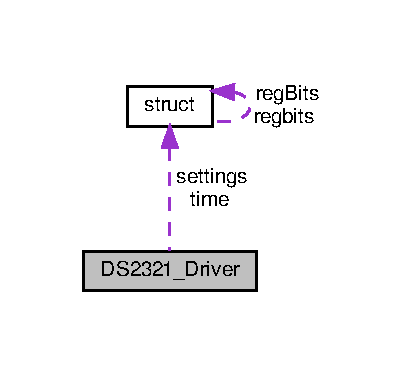
\includegraphics[width=194pt]{structDS2321__Driver__coll__graph}
\end{center}
\end{figure}
\subsection*{Public Attributes}
\begin{DoxyCompactItemize}
\item 
\mbox{\Hypertarget{structDS2321__Driver_a88591ce88d3acbd1822720ded9b982b1}\label{structDS2321__Driver_a88591ce88d3acbd1822720ded9b982b1}} 
\hyperlink{vl53l0x__types_8h_aba7bc1797add20fe3efdf37ced1182c5}{uint8\+\_\+t} {\bfseries i2c\+\_\+bus}
\item 
\mbox{\Hypertarget{structDS2321__Driver_a6e47c127b0ee78a273733b96bdde78d9}\label{structDS2321__Driver_a6e47c127b0ee78a273733b96bdde78d9}} 
Task\+Handle\+\_\+t {\bfseries t\+\_\+handle}
\item 
\mbox{\Hypertarget{structDS2321__Driver_a7d91bf719facb99a5781250810a8c07c}\label{structDS2321__Driver_a7d91bf719facb99a5781250810a8c07c}} 
\hyperlink{structDS2321__Time}{ds2321\+\_\+timedata\+\_\+t} {\bfseries time}
\item 
\mbox{\Hypertarget{structDS2321__Driver_a6671e5bc0dbd8ac9f8c248e99f34b432}\label{structDS2321__Driver_a6671e5bc0dbd8ac9f8c248e99f34b432}} 
\hyperlink{structDS2321__Settings}{ds2321\+\_\+settings\+\_\+t} {\bfseries settings}
\item 
\mbox{\Hypertarget{structDS2321__Driver_adabe3275e24e78a4e0c4b5560294e4b6}\label{structDS2321__Driver_adabe3275e24e78a4e0c4b5560294e4b6}} 
ds\+\_\+opmode\+\_\+t {\bfseries opmode}
\end{DoxyCompactItemize}


The documentation for this struct was generated from the following file\+:\begin{DoxyCompactItemize}
\item 
D\+S2321\+\_\+\+Driver/D\+S2321\+\_\+\+Driver.\+h\end{DoxyCompactItemize}

\hypertarget{structDS2321__Init}{}\section{D\+S2321\+\_\+\+Init Struct Reference}
\label{structDS2321__Init}\index{D\+S2321\+\_\+\+Init@{D\+S2321\+\_\+\+Init}}
\subsection*{Public Attributes}
\begin{DoxyCompactItemize}
\item 
\mbox{\Hypertarget{structDS2321__Init_ad1081923eb82a56140235ba76d92e6a8}\label{structDS2321__Init_ad1081923eb82a56140235ba76d92e6a8}} 
\hyperlink{vl53l0x__types_8h_aba7bc1797add20fe3efdf37ced1182c5}{uint8\+\_\+t} {\bfseries i2c\+\_\+bus}
\end{DoxyCompactItemize}


The documentation for this struct was generated from the following file\+:\begin{DoxyCompactItemize}
\item 
D\+S2321\+\_\+\+Driver/D\+S2321\+\_\+\+Driver.\+h\end{DoxyCompactItemize}

\hypertarget{structDS2321__Settings}{}\section{D\+S2321\+\_\+\+Settings Struct Reference}
\label{structDS2321__Settings}\index{D\+S2321\+\_\+\+Settings@{D\+S2321\+\_\+\+Settings}}
\subsection*{Public Attributes}
\begin{DoxyCompactItemize}
\item 
bool \hyperlink{structDS2321__Settings_a46b5b91d51365eaf7bdd500a73fb75ee}{twentyfour\+\_\+hour}
\end{DoxyCompactItemize}


\subsection{Member Data Documentation}
\mbox{\Hypertarget{structDS2321__Settings_a46b5b91d51365eaf7bdd500a73fb75ee}\label{structDS2321__Settings_a46b5b91d51365eaf7bdd500a73fb75ee}} 
\index{D\+S2321\+\_\+\+Settings@{D\+S2321\+\_\+\+Settings}!twentyfour\+\_\+hour@{twentyfour\+\_\+hour}}
\index{twentyfour\+\_\+hour@{twentyfour\+\_\+hour}!D\+S2321\+\_\+\+Settings@{D\+S2321\+\_\+\+Settings}}
\subsubsection{\texorpdfstring{twentyfour\+\_\+hour}{twentyfour\_hour}}
{\footnotesize\ttfamily bool D\+S2321\+\_\+\+Settings\+::twentyfour\+\_\+hour}

0 -\/ am/pm 1 -\/ 24hr 

The documentation for this struct was generated from the following file\+:\begin{DoxyCompactItemize}
\item 
D\+S2321\+\_\+\+Driver/D\+S2321\+\_\+\+Driver.\+h\end{DoxyCompactItemize}

\hypertarget{structDS2321__Time}{}\section{D\+S2321\+\_\+\+Time Struct Reference}
\label{structDS2321__Time}\index{D\+S2321\+\_\+\+Time@{D\+S2321\+\_\+\+Time}}
\subsection*{Public Attributes}
\begin{DoxyCompactItemize}
\item 
\mbox{\Hypertarget{structDS2321__Time_ae95c0b267aa6bf3568c3fcce1298872d}\label{structDS2321__Time_ae95c0b267aa6bf3568c3fcce1298872d}} 
\hyperlink{vl53l0x__types_8h_aba7bc1797add20fe3efdf37ced1182c5}{uint8\+\_\+t} {\bfseries seconds}
\item 
\mbox{\Hypertarget{structDS2321__Time_a3d7b7d99aef9efa2ee72bf14948e2622}\label{structDS2321__Time_a3d7b7d99aef9efa2ee72bf14948e2622}} 
\hyperlink{vl53l0x__types_8h_aba7bc1797add20fe3efdf37ced1182c5}{uint8\+\_\+t} {\bfseries minutes}
\item 
\mbox{\Hypertarget{structDS2321__Time_af857518f7cbb98dc3f96a32261789617}\label{structDS2321__Time_af857518f7cbb98dc3f96a32261789617}} 
\begin{tabbing}
xx\=xx\=xx\=xx\=xx\=xx\=xx\=xx\=xx\=\kill
union \{\\
\>\hyperlink{vl53l0x__types_8h_aba7bc1797add20fe3efdf37ced1182c5}{uint8\_t} {\bfseries hours\_12}\\
\>\hyperlink{vl53l0x__types_8h_aba7bc1797add20fe3efdf37ced1182c5}{uint8\_t} {\bfseries hours\_24}\\
\} {\bfseries hours}\\

\end{tabbing}\item 
\mbox{\Hypertarget{structDS2321__Time_ae1900a8be90f9b4af2d2c48a528f924c}\label{structDS2321__Time_ae1900a8be90f9b4af2d2c48a528f924c}} 
bool {\bfseries am}
\item 
\mbox{\Hypertarget{structDS2321__Time_a9771a605d3ca4b9ff10f97cef39035c8}\label{structDS2321__Time_a9771a605d3ca4b9ff10f97cef39035c8}} 
\hyperlink{vl53l0x__types_8h_aba7bc1797add20fe3efdf37ced1182c5}{uint8\+\_\+t} {\bfseries day}
\item 
\mbox{\Hypertarget{structDS2321__Time_a1aeaa5d8ade0a961af796c2f069c5dc6}\label{structDS2321__Time_a1aeaa5d8ade0a961af796c2f069c5dc6}} 
\hyperlink{vl53l0x__types_8h_aba7bc1797add20fe3efdf37ced1182c5}{uint8\+\_\+t} {\bfseries date}
\item 
\mbox{\Hypertarget{structDS2321__Time_a9dd138fdae805da5120814a0d1fd4d6f}\label{structDS2321__Time_a9dd138fdae805da5120814a0d1fd4d6f}} 
\hyperlink{vl53l0x__types_8h_aba7bc1797add20fe3efdf37ced1182c5}{uint8\+\_\+t} {\bfseries month}
\item 
\mbox{\Hypertarget{structDS2321__Time_a3e00887dce6436edf0950e4fed1919f0}\label{structDS2321__Time_a3e00887dce6436edf0950e4fed1919f0}} 
\hyperlink{vl53l0x__types_8h_a273cf69d639a59973b6019625df33e30}{uint16\+\_\+t} {\bfseries year}
\item 
\mbox{\Hypertarget{structDS2321__Time_a2ffd985e707057c218b807577f885874}\label{structDS2321__Time_a2ffd985e707057c218b807577f885874}} 
char {\bfseries day\+\_\+str} \mbox{[}16\mbox{]}
\item 
\mbox{\Hypertarget{structDS2321__Time_a3139ce6945405f54822e6c9c501f11d4}\label{structDS2321__Time_a3139ce6945405f54822e6c9c501f11d4}} 
char {\bfseries month\+\_\+str} \mbox{[}16\mbox{]}
\end{DoxyCompactItemize}


The documentation for this struct was generated from the following file\+:\begin{DoxyCompactItemize}
\item 
D\+S2321\+\_\+\+Driver/D\+S2321\+\_\+\+Driver.\+h\end{DoxyCompactItemize}

\hypertarget{structFSK__Register__Map}{}\section{F\+S\+K\+\_\+\+Register\+\_\+\+Map Struct Reference}
\label{structFSK__Register__Map}\index{F\+S\+K\+\_\+\+Register\+\_\+\+Map@{F\+S\+K\+\_\+\+Register\+\_\+\+Map}}


Collaboration diagram for F\+S\+K\+\_\+\+Register\+\_\+\+Map\+:\nopagebreak
\begin{figure}[H]
\begin{center}
\leavevmode
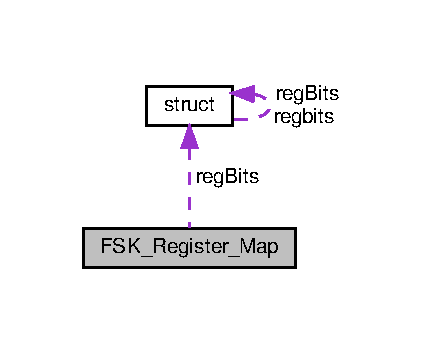
\includegraphics[width=204pt]{structFSK__Register__Map__coll__graph}
\end{center}
\end{figure}
\subsection*{Public Attributes}
\begin{DoxyCompactItemize}
\item 
\hyperlink{vl53l0x__types_8h_aba7bc1797add20fe3efdf37ced1182c5}{uint8\+\_\+t} \hyperlink{structFSK__Register__Map_af8d816816ccd860848376078e9c8b4b3}{reg\+Fifo}
\item 
\begin{tabbing}
xx\=xx\=xx\=xx\=xx\=xx\=xx\=xx\=xx\=\kill
union \{\\
\>\hyperlink{vl53l0x__types_8h_aba7bc1797add20fe3efdf37ced1182c5}{uint8\_t} {\bfseries regByte}\\
\>struct \{\\
\>\>\hyperlink{vl53l0x__types_8h_aba7bc1797add20fe3efdf37ced1182c5}{uint8\_t} {\bfseries mode}: 3\\
\>\>\hyperlink{vl53l0x__types_8h_aba7bc1797add20fe3efdf37ced1182c5}{uint8\_t} {\bfseries lowFreqModeEn}: 1\\
\>\>\hyperlink{vl53l0x__types_8h_aba7bc1797add20fe3efdf37ced1182c5}{uint8\_t} {\bfseries rsvd}: 1\\
\>\>\hyperlink{vl53l0x__types_8h_aba7bc1797add20fe3efdf37ced1182c5}{uint8\_t} {\bfseries modulationType}: 2\\
\>\>\hyperlink{vl53l0x__types_8h_aba7bc1797add20fe3efdf37ced1182c5}{uint8\_t} {\bfseries longRangeMode}: 1\\
\>\} {\bfseries regBits}\\
\} \hyperlink{structFSK__Register__Map_a80721749f8647cd67732a42b1f420678}{regOpMode}\\

\end{tabbing}\item 
\hyperlink{vl53l0x__types_8h_aba7bc1797add20fe3efdf37ced1182c5}{uint8\+\_\+t} \hyperlink{structFSK__Register__Map_a68832875d214893c0856a059988ecc7b}{reg\+Bitrate\+Msb}
\item 
\hyperlink{vl53l0x__types_8h_aba7bc1797add20fe3efdf37ced1182c5}{uint8\+\_\+t} \hyperlink{structFSK__Register__Map_a64b55aba43322c04e8233b10141abace}{reg\+Bitrate\+Lsb}
\item 
\begin{tabbing}
xx\=xx\=xx\=xx\=xx\=xx\=xx\=xx\=xx\=\kill
union \{\\
\>\hyperlink{vl53l0x__types_8h_aba7bc1797add20fe3efdf37ced1182c5}{uint8\_t} {\bfseries regByte}\\
\>struct \{\\
\>\>\hyperlink{vl53l0x__types_8h_aba7bc1797add20fe3efdf37ced1182c5}{uint8\_t} {\bfseries freqDevnMsb}: 6\\
\>\>\hyperlink{vl53l0x__types_8h_aba7bc1797add20fe3efdf37ced1182c5}{uint8\_t} {\bfseries resvd}: 2\\
\>\} {\bfseries regBits}\\
\} \hyperlink{structFSK__Register__Map_a62d7e754a10094746612f48825d87870}{regFreqDevnMsb}\\

\end{tabbing}\item 
\hyperlink{vl53l0x__types_8h_aba7bc1797add20fe3efdf37ced1182c5}{uint8\+\_\+t} \hyperlink{structFSK__Register__Map_a9265cac0c8d83f3c76e1a5fb5015ac88}{reg\+Freq\+Devn}
\item 
\hyperlink{vl53l0x__types_8h_aba7bc1797add20fe3efdf37ced1182c5}{uint8\+\_\+t} \hyperlink{structFSK__Register__Map_a84f971eeca1481b55775180b7f0b2594}{reg\+Rf\+Carrier\+Freq\+Msb}
\item 
\hyperlink{vl53l0x__types_8h_aba7bc1797add20fe3efdf37ced1182c5}{uint8\+\_\+t} \hyperlink{structFSK__Register__Map_a66036617e184731963f9539360b35de7}{reg\+Rf\+Carrier\+Freq\+Midsb}
\item 
\hyperlink{vl53l0x__types_8h_aba7bc1797add20fe3efdf37ced1182c5}{uint8\+\_\+t} \hyperlink{structFSK__Register__Map_aa44e65485b0af36e94eb0278b1dfe169}{reg\+Rf\+Carrier\+Freq\+Lsb}
\item 
\begin{tabbing}
xx\=xx\=xx\=xx\=xx\=xx\=xx\=xx\=xx\=\kill
union \{\\
\>\hyperlink{vl53l0x__types_8h_aba7bc1797add20fe3efdf37ced1182c5}{uint8\_t} {\bfseries regByte}\\
\>struct \{\\
\>\>\hyperlink{vl53l0x__types_8h_aba7bc1797add20fe3efdf37ced1182c5}{uint8\_t} {\bfseries outputPower}: 4\\
\>\>\hyperlink{vl53l0x__types_8h_aba7bc1797add20fe3efdf37ced1182c5}{uint8\_t} {\bfseries maxPower}: 3\\
\>\>\hyperlink{vl53l0x__types_8h_aba7bc1797add20fe3efdf37ced1182c5}{uint8\_t} {\bfseries pAmpSel}: 1\\
\>\} {\bfseries regBits}\\
\} \hyperlink{structFSK__Register__Map_a5f33d669890f7b2d49a00c705abcf87c}{regPwrAmpCfg}\\

\end{tabbing}\item 
\begin{tabbing}
xx\=xx\=xx\=xx\=xx\=xx\=xx\=xx\=xx\=\kill
union \{\\
\>\hyperlink{vl53l0x__types_8h_aba7bc1797add20fe3efdf37ced1182c5}{uint8\_t} {\bfseries regByte}\\
\>struct \{\\
\>\>\hyperlink{vl53l0x__types_8h_aba7bc1797add20fe3efdf37ced1182c5}{uint8\_t} {\bfseries paRamp}: 4\\
\>\>\hyperlink{vl53l0x__types_8h_aba7bc1797add20fe3efdf37ced1182c5}{uint8\_t} {\bfseries rsvd}: 1\\
\>\>\hyperlink{vl53l0x__types_8h_aba7bc1797add20fe3efdf37ced1182c5}{uint8\_t} {\bfseries modulationShape}: 2\\
\>\>\hyperlink{vl53l0x__types_8h_aba7bc1797add20fe3efdf37ced1182c5}{uint8\_t} {\bfseries unused}: 1\\
\>\} {\bfseries regBits}\\
\} \hyperlink{structFSK__Register__Map_aceb5d027a6484f87b90f5611c5efa8ce}{regPaRamp}\\

\end{tabbing}\item 
\begin{tabbing}
xx\=xx\=xx\=xx\=xx\=xx\=xx\=xx\=xx\=\kill
union \{\\
\>\hyperlink{vl53l0x__types_8h_aba7bc1797add20fe3efdf37ced1182c5}{uint8\_t} {\bfseries regByte}\\
\>struct \{\\
\>\>\hyperlink{vl53l0x__types_8h_aba7bc1797add20fe3efdf37ced1182c5}{uint8\_t} {\bfseries ocpTrim}: 4\\
\>\>\hyperlink{vl53l0x__types_8h_aba7bc1797add20fe3efdf37ced1182c5}{uint8\_t} {\bfseries ocpEn}: 1\\
\>\>\hyperlink{vl53l0x__types_8h_aba7bc1797add20fe3efdf37ced1182c5}{uint8\_t} {\bfseries unsused}: 2\\
\>\} {\bfseries regBits}\\
\} \hyperlink{structFSK__Register__Map_a0d9a922f0d94fe3b4be0ca67635e3877}{regOcp}\\

\end{tabbing}\item 
\begin{tabbing}
xx\=xx\=xx\=xx\=xx\=xx\=xx\=xx\=xx\=\kill
union \{\\
\>\hyperlink{vl53l0x__types_8h_aba7bc1797add20fe3efdf37ced1182c5}{uint8\_t} {\bfseries regByte}\\
\>struct \{\\
\>\>\hyperlink{vl53l0x__types_8h_aba7bc1797add20fe3efdf37ced1182c5}{uint8\_t} {\bfseries lnaBoostHFrq}: 2\\
\>\>\hyperlink{vl53l0x__types_8h_aba7bc1797add20fe3efdf37ced1182c5}{uint8\_t} {\bfseries rsvd}: 1\\
\>\>\hyperlink{vl53l0x__types_8h_aba7bc1797add20fe3efdf37ced1182c5}{uint8\_t} {\bfseries lnaBoostLFrq}: 2\\
\>\>\hyperlink{vl53l0x__types_8h_aba7bc1797add20fe3efdf37ced1182c5}{uint8\_t} {\bfseries lnaGain}: 3\\
\>\} {\bfseries regBits}\\
\} \hyperlink{structFSK__Register__Map_a07a3a4a108d6cce775cdc938a9837f87}{regLNA}\\

\end{tabbing}\item 
\begin{tabbing}
xx\=xx\=xx\=xx\=xx\=xx\=xx\=xx\=xx\=\kill
union \{\\
\>\hyperlink{vl53l0x__types_8h_aba7bc1797add20fe3efdf37ced1182c5}{uint8\_t} {\bfseries regByte}\\
\>struct \{\\
\>\>\hyperlink{vl53l0x__types_8h_aba7bc1797add20fe3efdf37ced1182c5}{uint8\_t} {\bfseries rxTrigger}: 3\\
\>\>\hyperlink{vl53l0x__types_8h_aba7bc1797add20fe3efdf37ced1182c5}{uint8\_t} {\bfseries agcAutoEn}: 1\\
\>\>\hyperlink{vl53l0x__types_8h_aba7bc1797add20fe3efdf37ced1182c5}{uint8\_t} {\bfseries afcAutoEn}: 1\\
\>\>\hyperlink{vl53l0x__types_8h_aba7bc1797add20fe3efdf37ced1182c5}{uint8\_t} {\bfseries restartRxWithPLL}: 1\\
\>\>\hyperlink{vl53l0x__types_8h_aba7bc1797add20fe3efdf37ced1182c5}{uint8\_t} {\bfseries restartRxWoPLL}: 1\\
\>\>\hyperlink{vl53l0x__types_8h_aba7bc1797add20fe3efdf37ced1182c5}{uint8\_t} {\bfseries restartRxOnCollision}: 1\\
\>\} {\bfseries regBits}\\
\} \hyperlink{structFSK__Register__Map_a0ed113da5f9c47e4f68ab98fefd48a1f}{regRxCfg}\\

\end{tabbing}\item 
\begin{tabbing}
xx\=xx\=xx\=xx\=xx\=xx\=xx\=xx\=xx\=\kill
union \{\\
\>\hyperlink{vl53l0x__types_8h_aba7bc1797add20fe3efdf37ced1182c5}{uint8\_t} {\bfseries regByte}\\
\>struct \{\\
\>\>\hyperlink{vl53l0x__types_8h_aba7bc1797add20fe3efdf37ced1182c5}{uint8\_t} {\bfseries rssiSmoothing}: 3\\
\>\>\hyperlink{vl53l0x__types_8h_aba7bc1797add20fe3efdf37ced1182c5}{uint8\_t} {\bfseries rssiOffset}: 5\\
\>\} {\bfseries regBits}\\
\} \hyperlink{structFSK__Register__Map_a79e4cf8525de96668c8d329c92fc587e}{regRssiCfg}\\

\end{tabbing}\item 
\hyperlink{vl53l0x__types_8h_aba7bc1797add20fe3efdf37ced1182c5}{uint8\+\_\+t} \hyperlink{structFSK__Register__Map_a5be388872ba759407950694b59a20b59}{rssi\+Collision\+Thresh}
\item 
\hyperlink{vl53l0x__types_8h_aba7bc1797add20fe3efdf37ced1182c5}{uint8\+\_\+t} \hyperlink{structFSK__Register__Map_ab02ef8f045c4ee796367f7f523b7bb03}{rssi\+Thresh}
\item 
\hyperlink{vl53l0x__types_8h_aba7bc1797add20fe3efdf37ced1182c5}{uint8\+\_\+t} \hyperlink{structFSK__Register__Map_a6046db82f7b1712785f20bd45a5fad62}{rssi\+Value}
\item 
\begin{tabbing}
xx\=xx\=xx\=xx\=xx\=xx\=xx\=xx\=xx\=\kill
union \{\\
\>\hyperlink{vl53l0x__types_8h_aba7bc1797add20fe3efdf37ced1182c5}{uint8\_t} {\bfseries regByte}\\
\>struct \{\\
\>\>\hyperlink{vl53l0x__types_8h_aba7bc1797add20fe3efdf37ced1182c5}{uint8\_t} {\bfseries rxBwExp}: 3\\
\>\>\hyperlink{vl53l0x__types_8h_aba7bc1797add20fe3efdf37ced1182c5}{uint8\_t} {\bfseries rxBwMan}: 2\\
\>\>\hyperlink{vl53l0x__types_8h_aba7bc1797add20fe3efdf37ced1182c5}{uint8\_t} {\bfseries rsvd}: 2\\
\>\>\hyperlink{vl53l0x__types_8h_aba7bc1797add20fe3efdf37ced1182c5}{uint8\_t} {\bfseries unused}: 1\\
\>\} {\bfseries regBits}\\
\} \hyperlink{structFSK__Register__Map_a6f8092f055bc1503936b4b38857de567}{regRxBw}\\

\end{tabbing}\item 
\begin{tabbing}
xx\=xx\=xx\=xx\=xx\=xx\=xx\=xx\=xx\=\kill
union \{\\
\>\hyperlink{vl53l0x__types_8h_aba7bc1797add20fe3efdf37ced1182c5}{uint8\_t} {\bfseries regByte}\\
\>struct \{\\
\>\>\hyperlink{vl53l0x__types_8h_aba7bc1797add20fe3efdf37ced1182c5}{uint8\_t} {\bfseries rxBwExpAft}: 3\\
\>\>\hyperlink{vl53l0x__types_8h_aba7bc1797add20fe3efdf37ced1182c5}{uint8\_t} {\bfseries rxBwMantAfc}: 2\\
\>\>\hyperlink{vl53l0x__types_8h_aba7bc1797add20fe3efdf37ced1182c5}{uint8\_t} {\bfseries rsvd}: 3\\
\>\} {\bfseries regBits}\\
\} \hyperlink{structFSK__Register__Map_a7dc528c9517c2f8a0dca679fac734d65}{regAfcBw}\\

\end{tabbing}\item 
\begin{tabbing}
xx\=xx\=xx\=xx\=xx\=xx\=xx\=xx\=xx\=\kill
union \{\\
\>\hyperlink{vl53l0x__types_8h_aba7bc1797add20fe3efdf37ced1182c5}{uint8\_t} {\bfseries regByte}\\
\>struct \{\\
\>\>\hyperlink{vl53l0x__types_8h_aba7bc1797add20fe3efdf37ced1182c5}{uint8\_t} {\bfseries ookPeakThreahStep}: 3\\
\>\>\hyperlink{vl53l0x__types_8h_aba7bc1797add20fe3efdf37ced1182c5}{uint8\_t} {\bfseries ookThreshType}: 2\\
\>\>\hyperlink{vl53l0x__types_8h_aba7bc1797add20fe3efdf37ced1182c5}{uint8\_t} {\bfseries bitSyncEn}: 1\\
\>\>\hyperlink{vl53l0x__types_8h_aba7bc1797add20fe3efdf37ced1182c5}{uint8\_t} {\bfseries rsvd}: 2\\
\>\} {\bfseries regBits}\\
\} \hyperlink{structFSK__Register__Map_aa9d2742d40ad17f24aacbf88098408a8}{regOokPeak}\\

\end{tabbing}\item 
\hyperlink{vl53l0x__types_8h_aba7bc1797add20fe3efdf37ced1182c5}{uint8\+\_\+t} \hyperlink{structFSK__Register__Map_ab3f42ae39895f99f4bbf807ba518a383}{reg\+O\+O\+K\+Fix}
\item 
\begin{tabbing}
xx\=xx\=xx\=xx\=xx\=xx\=xx\=xx\=xx\=\kill
union \{\\
\>\hyperlink{vl53l0x__types_8h_aba7bc1797add20fe3efdf37ced1182c5}{uint8\_t} {\bfseries regByte}\\
\>struct \{\\
\>\>\hyperlink{vl53l0x__types_8h_aba7bc1797add20fe3efdf37ced1182c5}{uint8\_t} {\bfseries ookAvgThreshFit}: 2\\
\>\>\hyperlink{vl53l0x__types_8h_aba7bc1797add20fe3efdf37ced1182c5}{uint8\_t} {\bfseries ookAvgOffset}: 2\\
\>\>\hyperlink{vl53l0x__types_8h_aba7bc1797add20fe3efdf37ced1182c5}{uint8\_t} {\bfseries rsvd}: 1\\
\>\>\hyperlink{vl53l0x__types_8h_aba7bc1797add20fe3efdf37ced1182c5}{uint8\_t} {\bfseries ookPeakThreshDecrm}: 3\\
\>\} {\bfseries regBits}\\
\} \hyperlink{structFSK__Register__Map_a8bc49b2b6b15dd9366328378bceb0c46}{regOOKAvg}\\

\end{tabbing}\item 
\hyperlink{vl53l0x__types_8h_aba7bc1797add20fe3efdf37ced1182c5}{uint8\+\_\+t} \hyperlink{structFSK__Register__Map_af7e323e294237445a51bb2e3ba715c87}{reg\+Rsvd17}
\item 
\hyperlink{vl53l0x__types_8h_aba7bc1797add20fe3efdf37ced1182c5}{uint8\+\_\+t} \hyperlink{structFSK__Register__Map_a83c29f2928c930890706ab7a8932b410}{reg\+Rsvd18}
\item 
\hyperlink{vl53l0x__types_8h_aba7bc1797add20fe3efdf37ced1182c5}{uint8\+\_\+t} \hyperlink{structFSK__Register__Map_aafef4fe23b36a7221a5b510a77f888ed}{reg\+Rsvd19}
\item 
\begin{tabbing}
xx\=xx\=xx\=xx\=xx\=xx\=xx\=xx\=xx\=\kill
union \{\\
\>\hyperlink{vl53l0x__types_8h_aba7bc1797add20fe3efdf37ced1182c5}{uint8\_t} {\bfseries regByte}\\
\>struct \{\\
\>\>\hyperlink{vl53l0x__types_8h_aba7bc1797add20fe3efdf37ced1182c5}{uint8\_t} {\bfseries afcAutoCleanEn}: 1\\
\>\>\hyperlink{vl53l0x__types_8h_aba7bc1797add20fe3efdf37ced1182c5}{uint8\_t} {\bfseries afcClear}: 1\\
\>\>\hyperlink{vl53l0x__types_8h_aba7bc1797add20fe3efdf37ced1182c5}{uint8\_t} {\bfseries unused2}: 1\\
\>\>\hyperlink{vl53l0x__types_8h_aba7bc1797add20fe3efdf37ced1182c5}{uint8\_t} {\bfseries rsvd}: 1\\
\>\>\hyperlink{vl53l0x__types_8h_aba7bc1797add20fe3efdf37ced1182c5}{uint8\_t} {\bfseries agcStart}: 1\\
\>\>\hyperlink{vl53l0x__types_8h_aba7bc1797add20fe3efdf37ced1182c5}{uint8\_t} {\bfseries unused}: 2\\
\>\} {\bfseries regBits}\\
\} \hyperlink{structFSK__Register__Map_a1d08787657f41411ea46bbe4a95dfde3}{regAfcFei}\\

\end{tabbing}\item 
\hyperlink{vl53l0x__types_8h_aba7bc1797add20fe3efdf37ced1182c5}{uint8\+\_\+t} \hyperlink{structFSK__Register__Map_affd05aea59c8554ad9ec8596d0e4bc4f}{reg\+Afc\+Msb}
\item 
\hyperlink{vl53l0x__types_8h_aba7bc1797add20fe3efdf37ced1182c5}{uint8\+\_\+t} \hyperlink{structFSK__Register__Map_a9e4aa98b29bf474fe44ad6a17b98930e}{reg\+Afc\+Lsb}
\item 
\hyperlink{vl53l0x__types_8h_aba7bc1797add20fe3efdf37ced1182c5}{uint8\+\_\+t} \hyperlink{structFSK__Register__Map_a5089be3b288eccb7a758e0c2ce874e3f}{reg\+Fei\+Msb}
\item 
\hyperlink{vl53l0x__types_8h_aba7bc1797add20fe3efdf37ced1182c5}{uint8\+\_\+t} \hyperlink{structFSK__Register__Map_a45a56b999282d713bd4cceb13d80c57a}{reg\+Fei\+Lsb}
\item 
\begin{tabbing}
xx\=xx\=xx\=xx\=xx\=xx\=xx\=xx\=xx\=\kill
union \{\\
\>\hyperlink{vl53l0x__types_8h_aba7bc1797add20fe3efdf37ced1182c5}{uint8\_t} {\bfseries regByte}\\
\>struct \{\\
\>\>\hyperlink{vl53l0x__types_8h_aba7bc1797add20fe3efdf37ced1182c5}{uint8\_t} {\bfseries preambleDetectorTln}: 5\\
\>\>\hyperlink{vl53l0x__types_8h_aba7bc1797add20fe3efdf37ced1182c5}{uint8\_t} {\bfseries preambleDetectorSize}: 2\\
\>\>\hyperlink{vl53l0x__types_8h_aba7bc1797add20fe3efdf37ced1182c5}{uint8\_t} {\bfseries preambleDetectorEn}: 1\\
\>\} {\bfseries regBits}\\
\} \hyperlink{structFSK__Register__Map_ace9b9c4930acfaa7153673072366fd53}{regPreambleDetect}\\

\end{tabbing}\item 
\hyperlink{vl53l0x__types_8h_aba7bc1797add20fe3efdf37ced1182c5}{uint8\+\_\+t} \hyperlink{structFSK__Register__Map_ae940a9518bc34cb8c24103dec37795ab}{reg\+Rx\+Timeout1}
\item 
\hyperlink{vl53l0x__types_8h_aba7bc1797add20fe3efdf37ced1182c5}{uint8\+\_\+t} \hyperlink{structFSK__Register__Map_ad6c65e197e7645e2522d86e7bf77b17e}{reg\+Rx\+Timeout2}
\item 
\hyperlink{vl53l0x__types_8h_aba7bc1797add20fe3efdf37ced1182c5}{uint8\+\_\+t} \hyperlink{structFSK__Register__Map_ac96c5de8da35af5700b9c8e14591071d}{reg\+Rx\+Timeout3}
\item 
\hyperlink{vl53l0x__types_8h_aba7bc1797add20fe3efdf37ced1182c5}{uint8\+\_\+t} \hyperlink{structFSK__Register__Map_a6d4235d2dd14a0f3a7798f97a45aa245}{reg\+Rx\+Delay}
\item 
\begin{tabbing}
xx\=xx\=xx\=xx\=xx\=xx\=xx\=xx\=xx\=\kill
union \{\\
\>\hyperlink{vl53l0x__types_8h_aba7bc1797add20fe3efdf37ced1182c5}{uint8\_t} {\bfseries regByte}\\
\>struct \{\\
\>\>\hyperlink{vl53l0x__types_8h_aba7bc1797add20fe3efdf37ced1182c5}{uint8\_t} {\bfseries clkOut}: 3\\
\>\>\hyperlink{vl53l0x__types_8h_aba7bc1797add20fe3efdf37ced1182c5}{uint8\_t} {\bfseries rcCalStart}: 1\\
\>\>\hyperlink{vl53l0x__types_8h_aba7bc1797add20fe3efdf37ced1182c5}{uint8\_t} {\bfseries unused}: 4\\
\>\} {\bfseries regBits}\\
\} \hyperlink{structFSK__Register__Map_aae9c8c9fe4a2cfd23aec8cc93cbb940d}{regOsc}\\

\end{tabbing}\item 
\hyperlink{vl53l0x__types_8h_aba7bc1797add20fe3efdf37ced1182c5}{uint8\+\_\+t} \hyperlink{structFSK__Register__Map_af81f911a0c63594bac0ef3f11085be01}{reg\+Preamble\+Msb}
\item 
\hyperlink{vl53l0x__types_8h_aba7bc1797add20fe3efdf37ced1182c5}{uint8\+\_\+t} \hyperlink{structFSK__Register__Map_a57cfe311a3ec957f1ec09f3637feaf5d}{reg\+Preamble\+Lsb}
\item 
\begin{tabbing}
xx\=xx\=xx\=xx\=xx\=xx\=xx\=xx\=xx\=\kill
union \{\\
\>\hyperlink{vl53l0x__types_8h_aba7bc1797add20fe3efdf37ced1182c5}{uint8\_t} {\bfseries regByte}\\
\>struct \{\\
\>\>\hyperlink{vl53l0x__types_8h_aba7bc1797add20fe3efdf37ced1182c5}{uint8\_t} {\bfseries syncSize}: 3\\
\>\>\hyperlink{vl53l0x__types_8h_aba7bc1797add20fe3efdf37ced1182c5}{uint8\_t} {\bfseries rsvd}: 1\\
\>\>\hyperlink{vl53l0x__types_8h_aba7bc1797add20fe3efdf37ced1182c5}{uint8\_t} {\bfseries syncEn}: 1\\
\>\>\hyperlink{vl53l0x__types_8h_aba7bc1797add20fe3efdf37ced1182c5}{uint8\_t} {\bfseries preamblePolarity}: 1\\
\>\>\hyperlink{vl53l0x__types_8h_aba7bc1797add20fe3efdf37ced1182c5}{uint8\_t} {\bfseries autoRestartRxMode}: 2\\
\>\} {\bfseries regBits}\\
\} \hyperlink{structFSK__Register__Map_a1007328afb50e8cb0d98daf772d3bfba}{regSyncCfg}\\

\end{tabbing}\item 
\hyperlink{vl53l0x__types_8h_aba7bc1797add20fe3efdf37ced1182c5}{uint8\+\_\+t} \hyperlink{structFSK__Register__Map_a90344919befe12b79b8663bb709ad16c}{reg\+Sync\+Value1}
\item 
\mbox{\Hypertarget{structFSK__Register__Map_aab876928974725f08a4d51ae609db4b2}\label{structFSK__Register__Map_aab876928974725f08a4d51ae609db4b2}} 
\hyperlink{vl53l0x__types_8h_aba7bc1797add20fe3efdf37ced1182c5}{uint8\+\_\+t} {\bfseries reg\+Sync\+Value2}
\item 
\mbox{\Hypertarget{structFSK__Register__Map_ab86af1f4e1e719b55c92388f6e77abbd}\label{structFSK__Register__Map_ab86af1f4e1e719b55c92388f6e77abbd}} 
\hyperlink{vl53l0x__types_8h_aba7bc1797add20fe3efdf37ced1182c5}{uint8\+\_\+t} {\bfseries reg\+Sync\+Value3}
\item 
\mbox{\Hypertarget{structFSK__Register__Map_a33732d17cd80589dd2d534fd88f75e13}\label{structFSK__Register__Map_a33732d17cd80589dd2d534fd88f75e13}} 
\hyperlink{vl53l0x__types_8h_aba7bc1797add20fe3efdf37ced1182c5}{uint8\+\_\+t} {\bfseries reg\+Sync\+Value4}
\item 
\mbox{\Hypertarget{structFSK__Register__Map_a8163d69c4d38ed5fcf5961d7483c70eb}\label{structFSK__Register__Map_a8163d69c4d38ed5fcf5961d7483c70eb}} 
\hyperlink{vl53l0x__types_8h_aba7bc1797add20fe3efdf37ced1182c5}{uint8\+\_\+t} {\bfseries reg\+Sync\+Value5}
\item 
\mbox{\Hypertarget{structFSK__Register__Map_af93cf44ae1a3e707c3db7d99c331797a}\label{structFSK__Register__Map_af93cf44ae1a3e707c3db7d99c331797a}} 
\hyperlink{vl53l0x__types_8h_aba7bc1797add20fe3efdf37ced1182c5}{uint8\+\_\+t} {\bfseries reg\+Sync\+Value6}
\item 
\mbox{\Hypertarget{structFSK__Register__Map_a1a4588791f5be6d5656bbcca2e0cefcf}\label{structFSK__Register__Map_a1a4588791f5be6d5656bbcca2e0cefcf}} 
\hyperlink{vl53l0x__types_8h_aba7bc1797add20fe3efdf37ced1182c5}{uint8\+\_\+t} {\bfseries reg\+Sync\+Value7}
\item 
\hyperlink{vl53l0x__types_8h_aba7bc1797add20fe3efdf37ced1182c5}{uint8\+\_\+t} \hyperlink{structFSK__Register__Map_a62821dfa5e5c3f9fd6b4f44afd6a692c}{reg\+Sync\+Value8}
\item 
\begin{tabbing}
xx\=xx\=xx\=xx\=xx\=xx\=xx\=xx\=xx\=\kill
union \{\\
\>\hyperlink{vl53l0x__types_8h_aba7bc1797add20fe3efdf37ced1182c5}{uint8\_t} {\bfseries regByte}\\
\>struct \{\\
\>\>\hyperlink{vl53l0x__types_8h_aba7bc1797add20fe3efdf37ced1182c5}{uint8\_t} {\bfseries crcWhiteType}: 1\\
\>\>\hyperlink{vl53l0x__types_8h_aba7bc1797add20fe3efdf37ced1182c5}{uint8\_t} {\bfseries addressFiltering}: 2\\
\>\>\hyperlink{vl53l0x__types_8h_aba7bc1797add20fe3efdf37ced1182c5}{uint8\_t} {\bfseries crcAutoClrOff}: 1\\
\>\>\hyperlink{vl53l0x__types_8h_aba7bc1797add20fe3efdf37ced1182c5}{uint8\_t} {\bfseries crcEn}: 1\\
\>\>\hyperlink{vl53l0x__types_8h_aba7bc1797add20fe3efdf37ced1182c5}{uint8\_t} {\bfseries dcFree}: 2\\
\>\>\hyperlink{vl53l0x__types_8h_aba7bc1797add20fe3efdf37ced1182c5}{uint8\_t} {\bfseries pktFormat}: 1\\
\>\} {\bfseries regBits}\\
\} \hyperlink{structFSK__Register__Map_a375ba9eac7b1a4f0e8dd6d7090f273d7}{regPacketCfg1}\\

\end{tabbing}\item 
\begin{tabbing}
xx\=xx\=xx\=xx\=xx\=xx\=xx\=xx\=xx\=\kill
union \{\\
\>\hyperlink{vl53l0x__types_8h_aba7bc1797add20fe3efdf37ced1182c5}{uint8\_t} {\bfseries regByte}\\
\>struct \{\\
\>\>\hyperlink{vl53l0x__types_8h_aba7bc1797add20fe3efdf37ced1182c5}{uint8\_t} {\bfseries payloadLenMsb}: 3\\
\>\>\hyperlink{vl53l0x__types_8h_aba7bc1797add20fe3efdf37ced1182c5}{uint8\_t} {\bfseries beaconEn}: 1\\
\>\>\hyperlink{vl53l0x__types_8h_aba7bc1797add20fe3efdf37ced1182c5}{uint8\_t} {\bfseries ioHomePwrFrame}: 1\\
\>\>\hyperlink{vl53l0x__types_8h_aba7bc1797add20fe3efdf37ced1182c5}{uint8\_t} {\bfseries ioHomeEn}: 1\\
\>\>\hyperlink{vl53l0x__types_8h_aba7bc1797add20fe3efdf37ced1182c5}{uint8\_t} {\bfseries dataMode}: 1\\
\>\>\hyperlink{vl53l0x__types_8h_aba7bc1797add20fe3efdf37ced1182c5}{uint8\_t} {\bfseries unused}: 1\\
\>\} {\bfseries regBits}\\
\} \hyperlink{structFSK__Register__Map_afd5db4f6d0024aaad38619378200742f}{regPacketCfg2}\\

\end{tabbing}\item 
\hyperlink{vl53l0x__types_8h_aba7bc1797add20fe3efdf37ced1182c5}{uint8\+\_\+t} \hyperlink{structFSK__Register__Map_a2ea93dabc539f284937ee5e4f4b128e7}{payload\+Len\+Lsb}
\item 
\hyperlink{vl53l0x__types_8h_aba7bc1797add20fe3efdf37ced1182c5}{uint8\+\_\+t} \hyperlink{structFSK__Register__Map_aa32b23b4a364b910d19374cdc406519d}{reg\+Node\+Address}
\item 
\hyperlink{vl53l0x__types_8h_aba7bc1797add20fe3efdf37ced1182c5}{uint8\+\_\+t} \hyperlink{structFSK__Register__Map_a4afcebd02b3b4e094b8d8908f46c50cb}{reg\+Broadcast\+Address}
\item 
\begin{tabbing}
xx\=xx\=xx\=xx\=xx\=xx\=xx\=xx\=xx\=\kill
union \{\\
\>\hyperlink{vl53l0x__types_8h_aba7bc1797add20fe3efdf37ced1182c5}{uint8\_t} {\bfseries regByte}\\
\>struct \{\\
\>\>\hyperlink{vl53l0x__types_8h_aba7bc1797add20fe3efdf37ced1182c5}{uint8\_t} {\bfseries fifoThresh}: 6\\
\>\>\hyperlink{vl53l0x__types_8h_aba7bc1797add20fe3efdf37ced1182c5}{uint8\_t} {\bfseries unused}: 1\\
\>\>\hyperlink{vl53l0x__types_8h_aba7bc1797add20fe3efdf37ced1182c5}{uint8\_t} {\bfseries txStartCondition}: 1\\
\>\} {\bfseries regBits}\\
\} \hyperlink{structFSK__Register__Map_a52834a7fbf201ad72d22f5946c2ebdc4}{regFifoThresh}\\

\end{tabbing}\item 
\begin{tabbing}
xx\=xx\=xx\=xx\=xx\=xx\=xx\=xx\=xx\=\kill
union \{\\
\>\hyperlink{vl53l0x__types_8h_aba7bc1797add20fe3efdf37ced1182c5}{uint8\_t} {\bfseries regByte}\\
\>struct \{\\
\>\>\hyperlink{vl53l0x__types_8h_aba7bc1797add20fe3efdf37ced1182c5}{uint8\_t} {\bfseries fromTransmit}: 1\\
\>\>\hyperlink{vl53l0x__types_8h_aba7bc1797add20fe3efdf37ced1182c5}{uint8\_t} {\bfseries fromIdle}: 1\\
\>\>\hyperlink{vl53l0x__types_8h_aba7bc1797add20fe3efdf37ced1182c5}{uint8\_t} {\bfseries lowPwrSelect}: 1\\
\>\>\hyperlink{vl53l0x__types_8h_aba7bc1797add20fe3efdf37ced1182c5}{uint8\_t} {\bfseries fromStart}: 2\\
\>\>\hyperlink{vl53l0x__types_8h_aba7bc1797add20fe3efdf37ced1182c5}{uint8\_t} {\bfseries idleMode}: 1\\
\>\>\hyperlink{vl53l0x__types_8h_aba7bc1797add20fe3efdf37ced1182c5}{uint8\_t} {\bfseries sequencerStop}: 1\\
\>\>\hyperlink{vl53l0x__types_8h_aba7bc1797add20fe3efdf37ced1182c5}{uint8\_t} {\bfseries sequencerStart}: 1\\
\>\} {\bfseries regBits}\\
\} \hyperlink{structFSK__Register__Map_ae90eb7c7055eab661ab05b8d8b8b1226}{regSequencerConf1}\\

\end{tabbing}\item 
\begin{tabbing}
xx\=xx\=xx\=xx\=xx\=xx\=xx\=xx\=xx\=\kill
union \{\\
\>\hyperlink{vl53l0x__types_8h_aba7bc1797add20fe3efdf37ced1182c5}{uint8\_t} {\bfseries regByte}\\
\>struct \{\\
\>\>\hyperlink{vl53l0x__types_8h_aba7bc1797add20fe3efdf37ced1182c5}{uint8\_t} {\bfseries fromPacketRcvd}: 3\\
\>\>\hyperlink{vl53l0x__types_8h_aba7bc1797add20fe3efdf37ced1182c5}{uint8\_t} {\bfseries fromRxTimeout}: 2\\
\>\>\hyperlink{vl53l0x__types_8h_aba7bc1797add20fe3efdf37ced1182c5}{uint8\_t} {\bfseries fromReceive}: 3\\
\>\} {\bfseries regBits}\\
\} \hyperlink{structFSK__Register__Map_a4f7376428f494fcc98e59d5c6b4454a8}{regSequencerCfg2}\\

\end{tabbing}\item 
\begin{tabbing}
xx\=xx\=xx\=xx\=xx\=xx\=xx\=xx\=xx\=\kill
union \{\\
\>\hyperlink{vl53l0x__types_8h_aba7bc1797add20fe3efdf37ced1182c5}{uint8\_t} {\bfseries regByte}\\
\>struct \{\\
\>\>\hyperlink{vl53l0x__types_8h_aba7bc1797add20fe3efdf37ced1182c5}{uint8\_t} {\bfseries timer2Resolution}: 2\\
\>\>\hyperlink{vl53l0x__types_8h_aba7bc1797add20fe3efdf37ced1182c5}{uint8\_t} {\bfseries timer1Resolution}: 2\\
\>\>\hyperlink{vl53l0x__types_8h_aba7bc1797add20fe3efdf37ced1182c5}{uint8\_t} {\bfseries unused}: 4\\
\>\} {\bfseries regBits}\\
\} \hyperlink{structFSK__Register__Map_a4f191c94ee411120b090f19acebdeb87}{regTimerResolution}\\

\end{tabbing}\item 
\hyperlink{vl53l0x__types_8h_aba7bc1797add20fe3efdf37ced1182c5}{uint8\+\_\+t} \hyperlink{structFSK__Register__Map_ac4d8dc321cd5cb47d5844a2882c81f11}{reg\+Timer1\+Coeff}
\item 
\hyperlink{vl53l0x__types_8h_aba7bc1797add20fe3efdf37ced1182c5}{uint8\+\_\+t} \hyperlink{structFSK__Register__Map_af69c2c867b524f2402499b5102d6384f}{reg\+Timer2\+Coeff}
\item 
\begin{tabbing}
xx\=xx\=xx\=xx\=xx\=xx\=xx\=xx\=xx\=\kill
union \{\\
\>\hyperlink{vl53l0x__types_8h_aba7bc1797add20fe3efdf37ced1182c5}{uint8\_t} {\bfseries regByte}\\
\>struct \{\\
\>\>\hyperlink{vl53l0x__types_8h_aba7bc1797add20fe3efdf37ced1182c5}{uint8\_t} {\bfseries tempMonitorOff}: 1\\
\>\>\hyperlink{vl53l0x__types_8h_aba7bc1797add20fe3efdf37ced1182c5}{uint8\_t} {\bfseries tempThresh}: 2\\
\>\>\hyperlink{vl53l0x__types_8h_aba7bc1797add20fe3efdf37ced1182c5}{uint8\_t} {\bfseries tempChange}: 1\\
\>\>\hyperlink{vl53l0x__types_8h_aba7bc1797add20fe3efdf37ced1182c5}{uint8\_t} {\bfseries unused}: 1\\
\>\>\hyperlink{vl53l0x__types_8h_aba7bc1797add20fe3efdf37ced1182c5}{uint8\_t} {\bfseries imageCalbrRunning}: 1\\
\>\>\hyperlink{vl53l0x__types_8h_aba7bc1797add20fe3efdf37ced1182c5}{uint8\_t} {\bfseries imageCalibrStart}: 1\\
\>\>\hyperlink{vl53l0x__types_8h_aba7bc1797add20fe3efdf37ced1182c5}{uint8\_t} {\bfseries autoImageCalEn}: 1\\
\>\} {\bfseries regBits}\\
\} \hyperlink{structFSK__Register__Map_a6bf176c426d56ef40727de470950b45d}{regImageCal}\\

\end{tabbing}\item 
\hyperlink{vl53l0x__types_8h_aba7bc1797add20fe3efdf37ced1182c5}{uint8\+\_\+t} \hyperlink{structFSK__Register__Map_abc6e3c39ab7c42dc2d404f96c706d3a0}{reg\+Temp}
\item 
\begin{tabbing}
xx\=xx\=xx\=xx\=xx\=xx\=xx\=xx\=xx\=\kill
union \{\\
\>\hyperlink{vl53l0x__types_8h_aba7bc1797add20fe3efdf37ced1182c5}{uint8\_t} {\bfseries regByte}\\
\>struct \{\\
\>\>\hyperlink{vl53l0x__types_8h_aba7bc1797add20fe3efdf37ced1182c5}{uint8\_t} {\bfseries lowBatTrim}: 3\\
\>\>\hyperlink{vl53l0x__types_8h_aba7bc1797add20fe3efdf37ced1182c5}{uint8\_t} {\bfseries lowBatEn}: 1\\
\>\>\hyperlink{vl53l0x__types_8h_aba7bc1797add20fe3efdf37ced1182c5}{uint8\_t} {\bfseries unused}: 4\\
\>\} {\bfseries regBits}\\
\} \hyperlink{structFSK__Register__Map_a275098e1838c38f4bad687b94880fcb6}{regLowBat}\\

\end{tabbing}\item 
\begin{tabbing}
xx\=xx\=xx\=xx\=xx\=xx\=xx\=xx\=xx\=\kill
union \{\\
\>\hyperlink{vl53l0x__types_8h_aba7bc1797add20fe3efdf37ced1182c5}{uint8\_t} {\bfseries regByte}\\
\>struct \{\\
\>\>\hyperlink{vl53l0x__types_8h_aba7bc1797add20fe3efdf37ced1182c5}{uint8\_t} {\bfseries syncAddrMatch}: 1\\
\>\>\hyperlink{vl53l0x__types_8h_aba7bc1797add20fe3efdf37ced1182c5}{uint8\_t} {\bfseries preambleDetect}: 1\\
\>\>\hyperlink{vl53l0x__types_8h_aba7bc1797add20fe3efdf37ced1182c5}{uint8\_t} {\bfseries timeout}: 1\\
\>\>\hyperlink{vl53l0x__types_8h_aba7bc1797add20fe3efdf37ced1182c5}{uint8\_t} {\bfseries rssi}: 1\\
\>\>\hyperlink{vl53l0x__types_8h_aba7bc1797add20fe3efdf37ced1182c5}{uint8\_t} {\bfseries pllLock}: 1\\
\>\>\hyperlink{vl53l0x__types_8h_aba7bc1797add20fe3efdf37ced1182c5}{uint8\_t} {\bfseries txReady}: 1\\
\>\>\hyperlink{vl53l0x__types_8h_aba7bc1797add20fe3efdf37ced1182c5}{uint8\_t} {\bfseries rxReady}: 1\\
\>\>\hyperlink{vl53l0x__types_8h_aba7bc1797add20fe3efdf37ced1182c5}{uint8\_t} {\bfseries modeReady}: 1\\
\>\} {\bfseries regBits}\\
\} \hyperlink{structFSK__Register__Map_abd981f959606f160c398fbcde8b2d2f7}{regIrqFlags1}\\

\end{tabbing}\item 
\begin{tabbing}
xx\=xx\=xx\=xx\=xx\=xx\=xx\=xx\=xx\=\kill
union \{\\
\>\hyperlink{vl53l0x__types_8h_aba7bc1797add20fe3efdf37ced1182c5}{uint8\_t} {\bfseries regByte}\\
\>struct \{\\
\>\>\hyperlink{vl53l0x__types_8h_aba7bc1797add20fe3efdf37ced1182c5}{uint8\_t} {\bfseries lowBat}: 1\\
\>\>\hyperlink{vl53l0x__types_8h_aba7bc1797add20fe3efdf37ced1182c5}{uint8\_t} {\bfseries crcOk}: 1\\
\>\>\hyperlink{vl53l0x__types_8h_aba7bc1797add20fe3efdf37ced1182c5}{uint8\_t} {\bfseries payloadready}: 1\\
\>\>\hyperlink{vl53l0x__types_8h_aba7bc1797add20fe3efdf37ced1182c5}{uint8\_t} {\bfseries packetSent}: 1\\
\>\>\hyperlink{vl53l0x__types_8h_aba7bc1797add20fe3efdf37ced1182c5}{uint8\_t} {\bfseries fifoOverrun}: 1\\
\>\>\hyperlink{vl53l0x__types_8h_aba7bc1797add20fe3efdf37ced1182c5}{uint8\_t} {\bfseries fifoLevel}: 1\\
\>\>\hyperlink{vl53l0x__types_8h_aba7bc1797add20fe3efdf37ced1182c5}{uint8\_t} {\bfseries fifoEmpty}: 1\\
\>\>\hyperlink{vl53l0x__types_8h_aba7bc1797add20fe3efdf37ced1182c5}{uint8\_t} {\bfseries fifoFull}: 1\\
\>\} {\bfseries regBits}\\
\} \hyperlink{structFSK__Register__Map_afbb4012b6fad4073630e742436a58937}{regIrqFlags2}\\

\end{tabbing}\item 
\begin{tabbing}
xx\=xx\=xx\=xx\=xx\=xx\=xx\=xx\=xx\=\kill
union \{\\
\>\hyperlink{vl53l0x__types_8h_aba7bc1797add20fe3efdf37ced1182c5}{uint8\_t} {\bfseries regByte}\\
\>struct \{\\
\>\>\hyperlink{vl53l0x__types_8h_aba7bc1797add20fe3efdf37ced1182c5}{uint8\_t} {\bfseries dio3mapping}: 2\\
\>\>\hyperlink{vl53l0x__types_8h_aba7bc1797add20fe3efdf37ced1182c5}{uint8\_t} {\bfseries dio2mapping}: 2\\
\>\>\hyperlink{vl53l0x__types_8h_aba7bc1797add20fe3efdf37ced1182c5}{uint8\_t} {\bfseries dio1mapping}: 2\\
\>\>\hyperlink{vl53l0x__types_8h_aba7bc1797add20fe3efdf37ced1182c5}{uint8\_t} {\bfseries dio0mapping}: 2\\
\>\} {\bfseries regBits}\\
\} \hyperlink{structFSK__Register__Map_a1bad09e60487d56039f110bde5bb51be}{regDioMapping1}\\

\end{tabbing}\item 
\begin{tabbing}
xx\=xx\=xx\=xx\=xx\=xx\=xx\=xx\=xx\=\kill
union \{\\
\>\hyperlink{vl53l0x__types_8h_aba7bc1797add20fe3efdf37ced1182c5}{uint8\_t} {\bfseries regByte}\\
\>struct \{\\
\>\>\hyperlink{vl53l0x__types_8h_aba7bc1797add20fe3efdf37ced1182c5}{uint8\_t} {\bfseries mapPreambleDetect}: 1\\
\>\>\hyperlink{vl53l0x__types_8h_aba7bc1797add20fe3efdf37ced1182c5}{uint8\_t} {\bfseries rsvd}: 3\\
\>\>\hyperlink{vl53l0x__types_8h_aba7bc1797add20fe3efdf37ced1182c5}{uint8\_t} {\bfseries dio5mapping}: 2\\
\>\>\hyperlink{vl53l0x__types_8h_aba7bc1797add20fe3efdf37ced1182c5}{uint8\_t} {\bfseries dio4mapping}: 2\\
\>\} {\bfseries regBits}\\
\} \hyperlink{structFSK__Register__Map_a759efaf7bc31c456f25300e2cec41f4c}{regDioMapping2}\\

\end{tabbing}\item 
\hyperlink{vl53l0x__types_8h_aba7bc1797add20fe3efdf37ced1182c5}{uint8\+\_\+t} \hyperlink{structFSK__Register__Map_afd8a85ac37879ffcb6238b5a6af1d3a0}{reg\+Version}
\item 
\hyperlink{vl53l0x__types_8h_aba7bc1797add20fe3efdf37ced1182c5}{uint8\+\_\+t} \hyperlink{structFSK__Register__Map_a6bf2a5eebe8ee09126136115f13b171d}{reg20rsvd}
\item 
\begin{tabbing}
xx\=xx\=xx\=xx\=xx\=xx\=xx\=xx\=xx\=\kill
union \{\\
\>\hyperlink{vl53l0x__types_8h_aba7bc1797add20fe3efdf37ced1182c5}{uint8\_t} {\bfseries regByte}\\
\>struct \{\\
\>\>\hyperlink{vl53l0x__types_8h_aba7bc1797add20fe3efdf37ced1182c5}{uint8\_t} {\bfseries rsvd}: 7\\
\>\>\hyperlink{vl53l0x__types_8h_aba7bc1797add20fe3efdf37ced1182c5}{uint8\_t} {\bfseries fastHopEn}: 1\\
\>\} {\bfseries regBits}\\
\} \hyperlink{structFSK__Register__Map_abbdf696294432f13a54dce470c386a92}{regPllHop}\\

\end{tabbing}\item 
\begin{tabbing}
xx\=xx\=xx\=xx\=xx\=xx\=xx\=xx\=xx\=\kill
union \{\\
\>\hyperlink{vl53l0x__types_8h_aba7bc1797add20fe3efdf37ced1182c5}{uint8\_t} {\bfseries regByte}\\
\>struct \{\\
\>\>\hyperlink{vl53l0x__types_8h_aba7bc1797add20fe3efdf37ced1182c5}{uint8\_t} {\bfseries rsvd0}: 4\\
\>\>\hyperlink{vl53l0x__types_8h_aba7bc1797add20fe3efdf37ced1182c5}{uint8\_t} {\bfseries txcoInputEn}: 1\\
\>\>\hyperlink{vl53l0x__types_8h_aba7bc1797add20fe3efdf37ced1182c5}{uint8\_t} {\bfseries rsvd1}: 3\\
\>\} {\bfseries regBits}\\
\} \hyperlink{structFSK__Register__Map_a8f7cbdb8a9512fe413105c1a653b8605}{regTxco}\\

\end{tabbing}\item 
\begin{tabbing}
xx\=xx\=xx\=xx\=xx\=xx\=xx\=xx\=xx\=\kill
union \{\\
\>\hyperlink{vl53l0x__types_8h_aba7bc1797add20fe3efdf37ced1182c5}{uint8\_t} {\bfseries regByte}\\
\>struct \{\\
\>\>\hyperlink{vl53l0x__types_8h_aba7bc1797add20fe3efdf37ced1182c5}{uint8\_t} {\bfseries paDac}: 3\\
\>\>\hyperlink{vl53l0x__types_8h_aba7bc1797add20fe3efdf37ced1182c5}{uint8\_t} {\bfseries rsvd}: 5\\
\>\} {\bfseries regBits}\\
\} \hyperlink{structFSK__Register__Map_ac0786829a2532811435e09eb8b62e1bf}{regPaDac}\\

\end{tabbing}\item 
\mbox{\Hypertarget{structFSK__Register__Map_aa15645edc079deb189e2515563cab9dc}\label{structFSK__Register__Map_aa15645edc079deb189e2515563cab9dc}} 
\hyperlink{vl53l0x__types_8h_aba7bc1797add20fe3efdf37ced1182c5}{uint8\+\_\+t} {\bfseries reg\+Former\+Temp}
\item 
\begin{tabbing}
xx\=xx\=xx\=xx\=xx\=xx\=xx\=xx\=xx\=\kill
union \{\\
\>\hyperlink{vl53l0x__types_8h_aba7bc1797add20fe3efdf37ced1182c5}{uint8\_t} {\bfseries regByte}\\
\>struct \{\\
\>\>\hyperlink{vl53l0x__types_8h_aba7bc1797add20fe3efdf37ced1182c5}{uint8\_t} {\bfseries bitRateFractional}: 4\\
\>\>\hyperlink{vl53l0x__types_8h_aba7bc1797add20fe3efdf37ced1182c5}{uint8\_t} {\bfseries unused}: 4\\
\>\} {\bfseries regBits}\\
\} \hyperlink{structFSK__Register__Map_a9fb3c91d923f38a0781d72dc438740fc}{regBitrateFrac}\\

\end{tabbing}\item 
\begin{tabbing}
xx\=xx\=xx\=xx\=xx\=xx\=xx\=xx\=xx\=\kill
union \{\\
\>\hyperlink{vl53l0x__types_8h_aba7bc1797add20fe3efdf37ced1182c5}{uint8\_t} {\bfseries regByte}\\
\>struct \{\\
\>\>\hyperlink{vl53l0x__types_8h_aba7bc1797add20fe3efdf37ced1182c5}{uint8\_t} {\bfseries agcReferenceLvl}: 6\\
\>\>\hyperlink{vl53l0x__types_8h_aba7bc1797add20fe3efdf37ced1182c5}{uint8\_t} {\bfseries unused}: 2\\
\>\} {\bfseries regBits}\\
\} \hyperlink{structFSK__Register__Map_a5a3ed3736aaa460bd9f816dfe47ed750}{regAgcRef}\\

\end{tabbing}\item 
\begin{tabbing}
xx\=xx\=xx\=xx\=xx\=xx\=xx\=xx\=xx\=\kill
union \{\\
\>\hyperlink{vl53l0x__types_8h_aba7bc1797add20fe3efdf37ced1182c5}{uint8\_t} {\bfseries regByte}\\
\>struct \{\\
\>\>\hyperlink{vl53l0x__types_8h_aba7bc1797add20fe3efdf37ced1182c5}{uint8\_t} {\bfseries agcStep1}: 4\\
\>\>\hyperlink{vl53l0x__types_8h_aba7bc1797add20fe3efdf37ced1182c5}{uint8\_t} {\bfseries unused}: 4\\
\>\} {\bfseries regBits}\\
\} \hyperlink{structFSK__Register__Map_a3fc08f679b041e6bd914bb9cfc112aee}{regAcgThresh1}\\

\end{tabbing}\item 
\begin{tabbing}
xx\=xx\=xx\=xx\=xx\=xx\=xx\=xx\=xx\=\kill
union \{\\
\>\hyperlink{vl53l0x__types_8h_aba7bc1797add20fe3efdf37ced1182c5}{uint8\_t} {\bfseries regByte}\\
\>struct \{\\
\>\>\hyperlink{vl53l0x__types_8h_aba7bc1797add20fe3efdf37ced1182c5}{uint8\_t} {\bfseries agcStep3}: 4\\
\>\>\hyperlink{vl53l0x__types_8h_aba7bc1797add20fe3efdf37ced1182c5}{uint8\_t} {\bfseries agcStep2}: 4\\
\>\} {\bfseries regBits}\\
\} \hyperlink{structFSK__Register__Map_a254ebf89525de4ef4174b4b59739edab}{regAgcThresh2}\\

\end{tabbing}\item 
\begin{tabbing}
xx\=xx\=xx\=xx\=xx\=xx\=xx\=xx\=xx\=\kill
union \{\\
\>\hyperlink{vl53l0x__types_8h_aba7bc1797add20fe3efdf37ced1182c5}{uint8\_t} {\bfseries regByte}\\
\>struct \{\\
\>\>\hyperlink{vl53l0x__types_8h_aba7bc1797add20fe3efdf37ced1182c5}{uint8\_t} {\bfseries agcStep5}: 4\\
\>\>\hyperlink{vl53l0x__types_8h_aba7bc1797add20fe3efdf37ced1182c5}{uint8\_t} {\bfseries agcStep4}: 4\\
\>\} {\bfseries regBits}\\
\} \hyperlink{structFSK__Register__Map_a391c957c12b3a7c63faa1788e4553704}{regAgcThresh3}\\

\end{tabbing}\item 
\begin{tabbing}
xx\=xx\=xx\=xx\=xx\=xx\=xx\=xx\=xx\=\kill
union \{\\
\>\hyperlink{vl53l0x__types_8h_aba7bc1797add20fe3efdf37ced1182c5}{uint8\_t} {\bfseries regByte}\\
\>struct \{\\
\>\>\hyperlink{vl53l0x__types_8h_aba7bc1797add20fe3efdf37ced1182c5}{uint8\_t} {\bfseries mode}: 3\\
\>\>\hyperlink{vl53l0x__types_8h_aba7bc1797add20fe3efdf37ced1182c5}{uint8\_t} {\bfseries lowFreqModeEn}: 1\\
\>\>\hyperlink{vl53l0x__types_8h_aba7bc1797add20fe3efdf37ced1182c5}{uint8\_t} {\bfseries rsvd}: 1\\
\>\>\hyperlink{vl53l0x__types_8h_aba7bc1797add20fe3efdf37ced1182c5}{uint8\_t} {\bfseries modulationType}: 2\\
\>\>\hyperlink{vl53l0x__types_8h_aba7bc1797add20fe3efdf37ced1182c5}{uint8\_t} {\bfseries longRangeMode}: 1\\
\>\} {\bfseries regBits}\\
\} \hyperlink{structFSK__Register__Map_a6a6a33fd7918a80851d0dcc6f9ee28b9}{regOpMode}\\

\end{tabbing}\item 
\hyperlink{vl53l0x__types_8h_aba7bc1797add20fe3efdf37ced1182c5}{uint8\+\_\+t} \hyperlink{structFSK__Register__Map_a85a8bc3f4fb36cb6aef3c265c23bc252}{unused02}
\item 
\hyperlink{vl53l0x__types_8h_aba7bc1797add20fe3efdf37ced1182c5}{uint8\+\_\+t} \hyperlink{structFSK__Register__Map_aa908432d1dbffcb64dbf8552da6dad22}{unused03}
\item 
\hyperlink{vl53l0x__types_8h_aba7bc1797add20fe3efdf37ced1182c5}{uint8\+\_\+t} \hyperlink{structFSK__Register__Map_ae27a2e44c6d1716aa2772ccb7b4a1968}{unused04}
\item 
\hyperlink{vl53l0x__types_8h_aba7bc1797add20fe3efdf37ced1182c5}{uint8\+\_\+t} \hyperlink{structFSK__Register__Map_a849022a1aa6af4524f2d10da17ea0171}{unused05}
\item 
\begin{tabbing}
xx\=xx\=xx\=xx\=xx\=xx\=xx\=xx\=xx\=\kill
union \{\\
\>\hyperlink{vl53l0x__types_8h_aba7bc1797add20fe3efdf37ced1182c5}{uint8\_t} {\bfseries regByte}\\
\>struct \{\\
\>\>\hyperlink{vl53l0x__types_8h_aba7bc1797add20fe3efdf37ced1182c5}{uint8\_t} {\bfseries outputPower}: 4\\
\>\>\hyperlink{vl53l0x__types_8h_aba7bc1797add20fe3efdf37ced1182c5}{uint8\_t} {\bfseries maxPower}: 3\\
\>\>\hyperlink{vl53l0x__types_8h_aba7bc1797add20fe3efdf37ced1182c5}{uint8\_t} {\bfseries pAmpSel}: 1\\
\>\} {\bfseries regBits}\\
\} \hyperlink{structFSK__Register__Map_a780d92c96bfd626d675d4406dd2dc742}{regPwrAmpCfg}\\

\end{tabbing}\item 
\begin{tabbing}
xx\=xx\=xx\=xx\=xx\=xx\=xx\=xx\=xx\=\kill
union \{\\
\>\hyperlink{vl53l0x__types_8h_aba7bc1797add20fe3efdf37ced1182c5}{uint8\_t} {\bfseries regByte}\\
\>struct \{\\
\>\>\hyperlink{vl53l0x__types_8h_aba7bc1797add20fe3efdf37ced1182c5}{uint8\_t} {\bfseries paRamp}: 4\\
\>\>\hyperlink{vl53l0x__types_8h_aba7bc1797add20fe3efdf37ced1182c5}{uint8\_t} {\bfseries rsvd}: 1\\
\>\>\hyperlink{vl53l0x__types_8h_aba7bc1797add20fe3efdf37ced1182c5}{uint8\_t} {\bfseries modulationShape}: 2\\
\>\>\hyperlink{vl53l0x__types_8h_aba7bc1797add20fe3efdf37ced1182c5}{uint8\_t} {\bfseries unused}: 1\\
\>\} {\bfseries regBits}\\
\} \hyperlink{structFSK__Register__Map_abacc022fe75b4791c52a1c0549ee45f9}{regPaRamp}\\

\end{tabbing}\item 
\begin{tabbing}
xx\=xx\=xx\=xx\=xx\=xx\=xx\=xx\=xx\=\kill
union \{\\
\>\hyperlink{vl53l0x__types_8h_aba7bc1797add20fe3efdf37ced1182c5}{uint8\_t} {\bfseries regByte}\\
\>struct \{\\
\>\>\hyperlink{vl53l0x__types_8h_aba7bc1797add20fe3efdf37ced1182c5}{uint8\_t} {\bfseries ocpTrim}: 4\\
\>\>\hyperlink{vl53l0x__types_8h_aba7bc1797add20fe3efdf37ced1182c5}{uint8\_t} {\bfseries ocpEn}: 1\\
\>\>\hyperlink{vl53l0x__types_8h_aba7bc1797add20fe3efdf37ced1182c5}{uint8\_t} {\bfseries unsused}: 2\\
\>\} {\bfseries regBits}\\
\} \hyperlink{structFSK__Register__Map_aa49ab7f4dd97ce2b98987c6a4f9b9ede}{regOcp}\\

\end{tabbing}\item 
\begin{tabbing}
xx\=xx\=xx\=xx\=xx\=xx\=xx\=xx\=xx\=\kill
union \{\\
\>\hyperlink{vl53l0x__types_8h_aba7bc1797add20fe3efdf37ced1182c5}{uint8\_t} {\bfseries regByte}\\
\>struct \{\\
\>\>\hyperlink{vl53l0x__types_8h_aba7bc1797add20fe3efdf37ced1182c5}{uint8\_t} {\bfseries lnaBoostHFrq}: 2\\
\>\>\hyperlink{vl53l0x__types_8h_aba7bc1797add20fe3efdf37ced1182c5}{uint8\_t} {\bfseries rsvd}: 1\\
\>\>\hyperlink{vl53l0x__types_8h_aba7bc1797add20fe3efdf37ced1182c5}{uint8\_t} {\bfseries lnaBoostLFrq}: 2\\
\>\>\hyperlink{vl53l0x__types_8h_aba7bc1797add20fe3efdf37ced1182c5}{uint8\_t} {\bfseries lnaGain}: 3\\
\>\} {\bfseries regBits}\\
\} \hyperlink{structFSK__Register__Map_afe20c0732a7f6fb5e2234a1253c46d2f}{regLNA}\\

\end{tabbing}\item 
\hyperlink{vl53l0x__types_8h_aba7bc1797add20fe3efdf37ced1182c5}{uint8\+\_\+t} \hyperlink{structFSK__Register__Map_acca50b6b3dacf0805dfbf5f125a7e513}{reg\+Fifo\+Addr\+Ptr}
\item 
\hyperlink{vl53l0x__types_8h_aba7bc1797add20fe3efdf37ced1182c5}{uint8\+\_\+t} \hyperlink{structFSK__Register__Map_ab2301d5a9696c7b28fa27539184c8b4a}{reg\+Fifo\+Tx\+Base\+Addr}
\item 
\hyperlink{vl53l0x__types_8h_aba7bc1797add20fe3efdf37ced1182c5}{uint8\+\_\+t} \hyperlink{structFSK__Register__Map_a62acebd7a0eab21ec4e8297e1343b403}{reg\+Fifo\+Rx\+Base\+Addr}
\item 
\hyperlink{vl53l0x__types_8h_aba7bc1797add20fe3efdf37ced1182c5}{uint8\+\_\+t} \hyperlink{structFSK__Register__Map_ad3c835e670be1d48e7d7c45f23b2d578}{reg\+Fifo\+Rx\+Curr\+Addr}
\item 
\begin{tabbing}
xx\=xx\=xx\=xx\=xx\=xx\=xx\=xx\=xx\=\kill
union \{\\
\>\hyperlink{vl53l0x__types_8h_aba7bc1797add20fe3efdf37ced1182c5}{uint8\_t} {\bfseries regByte}\\
\>struct \{\\
\>\>\hyperlink{vl53l0x__types_8h_aba7bc1797add20fe3efdf37ced1182c5}{uint8\_t} {\bfseries cadDetectedMask}: 1\\
\>\>\hyperlink{vl53l0x__types_8h_aba7bc1797add20fe3efdf37ced1182c5}{uint8\_t} {\bfseries fhssChgChnlMask}: 1\\
\>\>\hyperlink{vl53l0x__types_8h_aba7bc1797add20fe3efdf37ced1182c5}{uint8\_t} {\bfseries cadDoneMask}: 1\\
\>\>\hyperlink{vl53l0x__types_8h_aba7bc1797add20fe3efdf37ced1182c5}{uint8\_t} {\bfseries txDoneMask}: 1\\
\>\>\hyperlink{vl53l0x__types_8h_aba7bc1797add20fe3efdf37ced1182c5}{uint8\_t} {\bfseries validHeaderMask}: 1\\
\>\>\hyperlink{vl53l0x__types_8h_aba7bc1797add20fe3efdf37ced1182c5}{uint8\_t} {\bfseries payloadCrcErrorMask}: 1\\
\>\>\hyperlink{vl53l0x__types_8h_aba7bc1797add20fe3efdf37ced1182c5}{uint8\_t} {\bfseries rxDoneMask}: 1\\
\>\>\hyperlink{vl53l0x__types_8h_aba7bc1797add20fe3efdf37ced1182c5}{uint8\_t} {\bfseries rxTimeoutMask}: 1\\
\>\} {\bfseries regBits}\\
\} \hyperlink{structFSK__Register__Map_a0d7ff48d3b38bbe8f82b326d70e20f60}{regIrqFlagsMask}\\

\end{tabbing}\item 
\begin{tabbing}
xx\=xx\=xx\=xx\=xx\=xx\=xx\=xx\=xx\=\kill
union \{\\
\>\hyperlink{vl53l0x__types_8h_aba7bc1797add20fe3efdf37ced1182c5}{uint8\_t} {\bfseries regByte}\\
\>struct \{\\
\>\>\hyperlink{vl53l0x__types_8h_aba7bc1797add20fe3efdf37ced1182c5}{uint8\_t} {\bfseries cadDetected}: 1\\
\>\>\hyperlink{vl53l0x__types_8h_aba7bc1797add20fe3efdf37ced1182c5}{uint8\_t} {\bfseries validHeader}: 1\\
\>\>\hyperlink{vl53l0x__types_8h_aba7bc1797add20fe3efdf37ced1182c5}{uint8\_t} {\bfseries payloadCrcError}: 1\\
\>\>\hyperlink{vl53l0x__types_8h_aba7bc1797add20fe3efdf37ced1182c5}{uint8\_t} {\bfseries txDone}: 1\\
\>\>\hyperlink{vl53l0x__types_8h_aba7bc1797add20fe3efdf37ced1182c5}{uint8\_t} {\bfseries rxDone}: 1\\
\>\>\hyperlink{vl53l0x__types_8h_aba7bc1797add20fe3efdf37ced1182c5}{uint8\_t} {\bfseries cadDone}: 1\\
\>\>\hyperlink{vl53l0x__types_8h_aba7bc1797add20fe3efdf37ced1182c5}{uint8\_t} {\bfseries fhssChgChnl}: 1\\
\>\>\hyperlink{vl53l0x__types_8h_aba7bc1797add20fe3efdf37ced1182c5}{uint8\_t} {\bfseries rxTimeout}: 1\\
\>\} {\bfseries regBits}\\
\} \hyperlink{structFSK__Register__Map_acd1b988c5c5cf64b7a5e33640fd4e2e3}{regIrqFlags}\\

\end{tabbing}\item 
\hyperlink{vl53l0x__types_8h_aba7bc1797add20fe3efdf37ced1182c5}{uint8\+\_\+t} \hyperlink{structFSK__Register__Map_ace65e31341b842864ace8d4a570cdb23}{reg\+Rx\+Num\+Bytes}
\item 
\hyperlink{vl53l0x__types_8h_aba7bc1797add20fe3efdf37ced1182c5}{uint8\+\_\+t} \hyperlink{structFSK__Register__Map_ad7264b2a5ec03c9466d345cd5f41981e}{reg\+Rx\+Hdr\+Cnt\+Msb}
\item 
\hyperlink{vl53l0x__types_8h_aba7bc1797add20fe3efdf37ced1182c5}{uint8\+\_\+t} \hyperlink{structFSK__Register__Map_a31e12c2d2af69fa4c871e2f7e0e3517b}{reg\+Rx\+Hdr\+Cnt\+Lsb}
\item 
\hyperlink{vl53l0x__types_8h_aba7bc1797add20fe3efdf37ced1182c5}{uint8\+\_\+t} \hyperlink{structFSK__Register__Map_a02115927afb203d802796d3b76395a51}{reg\+Rx\+Pkt\+Cnt\+Msb}
\item 
\hyperlink{vl53l0x__types_8h_aba7bc1797add20fe3efdf37ced1182c5}{uint8\+\_\+t} \hyperlink{structFSK__Register__Map_adb4b4e071c4c37b27273cb49b9e2fa12}{reg\+Rx\+Pkt\+Cnt\+Lsb}
\item 
\begin{tabbing}
xx\=xx\=xx\=xx\=xx\=xx\=xx\=xx\=xx\=\kill
union \{\\
\>\hyperlink{vl53l0x__types_8h_aba7bc1797add20fe3efdf37ced1182c5}{uint8\_t} {\bfseries regByte}\\
\>struct \{\\
\>\>\hyperlink{vl53l0x__types_8h_aba7bc1797add20fe3efdf37ced1182c5}{uint8\_t} {\bfseries modemStatus}: 5\\
\>\>\hyperlink{vl53l0x__types_8h_aba7bc1797add20fe3efdf37ced1182c5}{uint8\_t} {\bfseries rxCodingRate}: 3\\
\>\} {\bfseries regBits}\\
\} \hyperlink{structFSK__Register__Map_a66a0df0ff7c5fb1892058ff0be454ed4}{regModemStatus}\\

\end{tabbing}\item 
\hyperlink{vl53l0x__types_8h_aba7bc1797add20fe3efdf37ced1182c5}{uint8\+\_\+t} \hyperlink{structFSK__Register__Map_a92cd6ce02538704e0e27d117099e4775}{reg\+Pkt\+Snr\+Value}
\item 
\hyperlink{vl53l0x__types_8h_aba7bc1797add20fe3efdf37ced1182c5}{uint8\+\_\+t} \hyperlink{structFSK__Register__Map_a019593bb7007a2b7d67e5565d565c5f8}{reg\+Pkt\+Rssi\+Value}
\item 
\hyperlink{vl53l0x__types_8h_aba7bc1797add20fe3efdf37ced1182c5}{uint8\+\_\+t} \hyperlink{structFSK__Register__Map_af6af2ecacf804bbab3b46c3f52a13b3f}{reg\+Rssi\+Value}
\item 
\begin{tabbing}
xx\=xx\=xx\=xx\=xx\=xx\=xx\=xx\=xx\=\kill
union \{\\
\>\hyperlink{vl53l0x__types_8h_aba7bc1797add20fe3efdf37ced1182c5}{uint8\_t} {\bfseries regByte}\\
\>struct \{\\
\>\>\hyperlink{vl53l0x__types_8h_aba7bc1797add20fe3efdf37ced1182c5}{uint8\_t} {\bfseries fhssPresentChannel}: 6\\
\>\>\hyperlink{vl53l0x__types_8h_aba7bc1797add20fe3efdf37ced1182c5}{uint8\_t} {\bfseries crcOnPayload}: 1\\
\>\>\hyperlink{vl53l0x__types_8h_aba7bc1797add20fe3efdf37ced1182c5}{uint8\_t} {\bfseries pllTimeout}: 1\\
\>\} {\bfseries regBits}\\
\} \hyperlink{structFSK__Register__Map_a881587e6b5cba28da6300ec6e1f9e9ee}{regHopChannel}\\

\end{tabbing}\item 
\begin{tabbing}
xx\=xx\=xx\=xx\=xx\=xx\=xx\=xx\=xx\=\kill
union \{\\
\>\hyperlink{vl53l0x__types_8h_aba7bc1797add20fe3efdf37ced1182c5}{uint8\_t} {\bfseries regByte}\\
\>struct \{\\
\>\>\hyperlink{vl53l0x__types_8h_aba7bc1797add20fe3efdf37ced1182c5}{uint8\_t} {\bfseries implicitHdrModeEn}: 1\\
\>\>\hyperlink{vl53l0x__types_8h_aba7bc1797add20fe3efdf37ced1182c5}{uint8\_t} {\bfseries codingRate}: 3\\
\>\>\hyperlink{vl53l0x__types_8h_aba7bc1797add20fe3efdf37ced1182c5}{uint8\_t} {\bfseries bandwidth}: 4\\
\>\} {\bfseries regBits}\\
\} \hyperlink{structFSK__Register__Map_a473a9661c49b5a2e0aab4ff816591a41}{regModemCfg1}\\

\end{tabbing}\item 
\begin{tabbing}
xx\=xx\=xx\=xx\=xx\=xx\=xx\=xx\=xx\=\kill
union \{\\
\>\hyperlink{vl53l0x__types_8h_aba7bc1797add20fe3efdf37ced1182c5}{uint8\_t} {\bfseries regByte}\\
\>struct \{\\
\>\>\hyperlink{vl53l0x__types_8h_aba7bc1797add20fe3efdf37ced1182c5}{uint8\_t} {\bfseries symbTimeout}: 2\\
\>\>\hyperlink{vl53l0x__types_8h_aba7bc1797add20fe3efdf37ced1182c5}{uint8\_t} {\bfseries rxPayloadCrcEn}: 1\\
\>\>\hyperlink{vl53l0x__types_8h_aba7bc1797add20fe3efdf37ced1182c5}{uint8\_t} {\bfseries txContinuousMode}: 1\\
\>\>\hyperlink{vl53l0x__types_8h_aba7bc1797add20fe3efdf37ced1182c5}{uint8\_t} {\bfseries spreadingFactor}: 4\\
\>\} {\bfseries regBits}\\
\} \hyperlink{structFSK__Register__Map_ace2901b2090c4b1a80ecf5ce1f67148f}{regModemCfg2}\\

\end{tabbing}\item 
\hyperlink{vl53l0x__types_8h_aba7bc1797add20fe3efdf37ced1182c5}{uint8\+\_\+t} \hyperlink{structFSK__Register__Map_ade9a79744d1c2e13a02616816235df2d}{reg\+Symb\+Timeout}
\item 
\hyperlink{vl53l0x__types_8h_aba7bc1797add20fe3efdf37ced1182c5}{uint8\+\_\+t} \hyperlink{structFSK__Register__Map_aef9ecfdf52f3408be54c23257b052736}{reg\+Max\+Payload\+Len}
\item 
\hyperlink{vl53l0x__types_8h_aba7bc1797add20fe3efdf37ced1182c5}{uint8\+\_\+t} \hyperlink{structFSK__Register__Map_a32ae7db6dec77f2f468661db51c3de8f}{reg\+Payload\+Len}
\item 
\hyperlink{vl53l0x__types_8h_aba7bc1797add20fe3efdf37ced1182c5}{uint8\+\_\+t} \hyperlink{structFSK__Register__Map_a891dfd7541ddaf01d15ab6c757c737ba}{reg\+Hop\+Period}
\item 
\hyperlink{vl53l0x__types_8h_aba7bc1797add20fe3efdf37ced1182c5}{uint8\+\_\+t} \hyperlink{structFSK__Register__Map_a2cc794150b2e012e12199aeb6a6e43ce}{reg\+Fifo\+Rx\+Byte\+Addr}
\item 
\begin{tabbing}
xx\=xx\=xx\=xx\=xx\=xx\=xx\=xx\=xx\=\kill
union \{\\
\>\hyperlink{vl53l0x__types_8h_aba7bc1797add20fe3efdf37ced1182c5}{uint8\_t} {\bfseries regByte}\\
\>struct \{\\
\>\>\hyperlink{vl53l0x__types_8h_aba7bc1797add20fe3efdf37ced1182c5}{uint8\_t} {\bfseries rsvd}: 2\\
\>\>\hyperlink{vl53l0x__types_8h_aba7bc1797add20fe3efdf37ced1182c5}{uint8\_t} {\bfseries agcAutoEn}: 1\\
\>\>\hyperlink{vl53l0x__types_8h_aba7bc1797add20fe3efdf37ced1182c5}{uint8\_t} {\bfseries lowDataRateOptEn}: 1\\
\>\>\hyperlink{vl53l0x__types_8h_aba7bc1797add20fe3efdf37ced1182c5}{uint8\_t} {\bfseries unused}: 4\\
\>\} {\bfseries regBits}\\
\} \hyperlink{structFSK__Register__Map_ac3f389d123f03e183b78d3d5afc38107}{regModemConfig3}\\

\end{tabbing}\item 
\hyperlink{vl53l0x__types_8h_aba7bc1797add20fe3efdf37ced1182c5}{uint8\+\_\+t} \hyperlink{structFSK__Register__Map_ac69ff074c058d20d6947655b20a4f636}{reg\+Ppm\+Correction}
\item 
\begin{tabbing}
xx\=xx\=xx\=xx\=xx\=xx\=xx\=xx\=xx\=\kill
union \{\\
\>\hyperlink{vl53l0x__types_8h_aba7bc1797add20fe3efdf37ced1182c5}{uint8\_t} {\bfseries regByte}\\
\>struct \{\\
\>\>\hyperlink{vl53l0x__types_8h_aba7bc1797add20fe3efdf37ced1182c5}{uint8\_t} {\bfseries freqErrorMsb}: 4\\
\>\>\hyperlink{vl53l0x__types_8h_aba7bc1797add20fe3efdf37ced1182c5}{uint8\_t} {\bfseries rsvd}: 4\\
\>\} {\bfseries regBits}\\
\} \hyperlink{structFSK__Register__Map_a17653fab98463c389e0e1bae3a2d3f21}{regFeiMsb}\\

\end{tabbing}\item 
\hyperlink{vl53l0x__types_8h_aba7bc1797add20fe3efdf37ced1182c5}{uint8\+\_\+t} \hyperlink{structFSK__Register__Map_a42a7660244fc2d4b00bb2621f956f7a6}{reg\+Fei\+Midsb}
\item 
\hyperlink{vl53l0x__types_8h_aba7bc1797add20fe3efdf37ced1182c5}{uint8\+\_\+t} \hyperlink{structFSK__Register__Map_aeacf91b2a66c8aa68397e30e9a2bb654}{rsvd2b}
\item 
\hyperlink{vl53l0x__types_8h_aba7bc1797add20fe3efdf37ced1182c5}{uint8\+\_\+t} \hyperlink{structFSK__Register__Map_a8ef62369a6e1d9dfc9b477d7364fbd47}{reg\+Rssi\+Wideband}
\item 
\hyperlink{vl53l0x__types_8h_aba7bc1797add20fe3efdf37ced1182c5}{uint8\+\_\+t} \hyperlink{structFSK__Register__Map_a74dae9aa81722ee02841bb6a31e81ff1}{rsvd2d}
\item 
\mbox{\Hypertarget{structFSK__Register__Map_a4610d1a13cd9709d35f1d8bad6334a3d}\label{structFSK__Register__Map_a4610d1a13cd9709d35f1d8bad6334a3d}} 
\hyperlink{vl53l0x__types_8h_aba7bc1797add20fe3efdf37ced1182c5}{uint8\+\_\+t} {\bfseries rsvd2e}
\item 
\mbox{\Hypertarget{structFSK__Register__Map_a01cbf61cc7bc7bee29057e9852d131e7}\label{structFSK__Register__Map_a01cbf61cc7bc7bee29057e9852d131e7}} 
\hyperlink{vl53l0x__types_8h_aba7bc1797add20fe3efdf37ced1182c5}{uint8\+\_\+t} {\bfseries rsvd2f}
\item 
\mbox{\Hypertarget{structFSK__Register__Map_a4b0c76a1cad529cedf0ec18c8ab0ad86}\label{structFSK__Register__Map_a4b0c76a1cad529cedf0ec18c8ab0ad86}} 
\hyperlink{vl53l0x__types_8h_aba7bc1797add20fe3efdf37ced1182c5}{uint8\+\_\+t} {\bfseries rsvd30}
\item 
\begin{tabbing}
xx\=xx\=xx\=xx\=xx\=xx\=xx\=xx\=xx\=\kill
union \{\\
\>\hyperlink{vl53l0x__types_8h_aba7bc1797add20fe3efdf37ced1182c5}{uint8\_t} {\bfseries regByte}\\
\>struct \{\\
\>\>\hyperlink{vl53l0x__types_8h_aba7bc1797add20fe3efdf37ced1182c5}{uint8\_t} {\bfseries detectOptmz}: 3\\
\>\>\hyperlink{vl53l0x__types_8h_aba7bc1797add20fe3efdf37ced1182c5}{uint8\_t} {\bfseries rsvd}: 5\\
\>\} {\bfseries regBits}\\
\} \hyperlink{structFSK__Register__Map_af34ed65b16362f5e7e19bcb397f7dd84}{regDetectOptmz}\\

\end{tabbing}\item 
\hyperlink{vl53l0x__types_8h_aba7bc1797add20fe3efdf37ced1182c5}{uint8\+\_\+t} \hyperlink{structFSK__Register__Map_a2afb62dfcde2ff0b44bd883947289d33}{rsvd32}
\item 
\begin{tabbing}
xx\=xx\=xx\=xx\=xx\=xx\=xx\=xx\=xx\=\kill
union \{\\
\>\hyperlink{vl53l0x__types_8h_aba7bc1797add20fe3efdf37ced1182c5}{uint8\_t} {\bfseries regByte}\\
\>struct \{\\
\>\>\hyperlink{vl53l0x__types_8h_aba7bc1797add20fe3efdf37ced1182c5}{uint8\_t} {\bfseries rsvd0}: 6\\
\>\>\hyperlink{vl53l0x__types_8h_aba7bc1797add20fe3efdf37ced1182c5}{uint8\_t} {\bfseries invertIq}: 1\\
\>\>\hyperlink{vl53l0x__types_8h_aba7bc1797add20fe3efdf37ced1182c5}{uint8\_t} {\bfseries rsvd1}: 1\\
\>\} {\bfseries regBits}\\
\} \hyperlink{structFSK__Register__Map_a0d59eab2b1fd415bf69d2ab31c8e3814}{regInvertIq}\\

\end{tabbing}\item 
\hyperlink{vl53l0x__types_8h_aba7bc1797add20fe3efdf37ced1182c5}{uint8\+\_\+t} \hyperlink{structFSK__Register__Map_a1a2c58e0776b3a2e11da16f8375322d1}{rsvd34}
\item 
\hyperlink{vl53l0x__types_8h_aba7bc1797add20fe3efdf37ced1182c5}{uint8\+\_\+t} \hyperlink{structFSK__Register__Map_ade667a254bb12ea7f56d08d208ba5160}{rsvd35}
\item 
\hyperlink{vl53l0x__types_8h_aba7bc1797add20fe3efdf37ced1182c5}{uint8\+\_\+t} \hyperlink{structFSK__Register__Map_a3d406fe0573250f10a884e8d161639b3}{rsvd36}
\item 
\hyperlink{vl53l0x__types_8h_aba7bc1797add20fe3efdf37ced1182c5}{uint8\+\_\+t} \hyperlink{structFSK__Register__Map_a1732d260747bbc5f55cc99d8c237bf5b}{reg\+Detect\+Thresh}
\item 
\hyperlink{vl53l0x__types_8h_aba7bc1797add20fe3efdf37ced1182c5}{uint8\+\_\+t} \hyperlink{structFSK__Register__Map_a7bfcdda86b67f7cb80acf251903197e6}{rsvd38}
\item 
\hyperlink{vl53l0x__types_8h_aba7bc1797add20fe3efdf37ced1182c5}{uint8\+\_\+t} \hyperlink{structFSK__Register__Map_a0fc3c281bcbeaea3ace8165414bed92d}{reg\+Sync\+Word}
\item 
\hyperlink{vl53l0x__types_8h_aba7bc1797add20fe3efdf37ced1182c5}{uint8\+\_\+t} \hyperlink{structFSK__Register__Map_a1566b81594323d9f4ac2374f8260b0c5}{rsvd3a}
\item 
\hyperlink{vl53l0x__types_8h_aba7bc1797add20fe3efdf37ced1182c5}{uint8\+\_\+t} \hyperlink{structFSK__Register__Map_ab0dc3c7ae155ebbadabae5f641676ae8}{rsvd3b}
\item 
\hyperlink{vl53l0x__types_8h_aba7bc1797add20fe3efdf37ced1182c5}{uint8\+\_\+t} \hyperlink{structFSK__Register__Map_abf24aaa2047e26a37afa89074c58368a}{rsvd3c}
\item 
\hyperlink{vl53l0x__types_8h_aba7bc1797add20fe3efdf37ced1182c5}{uint8\+\_\+t} \hyperlink{structFSK__Register__Map_a6f525cad38de316666645bed27fd7615}{rsvd3d}
\item 
\hyperlink{vl53l0x__types_8h_aba7bc1797add20fe3efdf37ced1182c5}{uint8\+\_\+t} \hyperlink{structFSK__Register__Map_ab645e8830b17d42f2e0b2d3f750c0f70}{rsvd3e}
\item 
\hyperlink{vl53l0x__types_8h_aba7bc1797add20fe3efdf37ced1182c5}{uint8\+\_\+t} \hyperlink{structFSK__Register__Map_abc63838e4050030d45da25ab44964c80}{rsvd3f}
\item 
\begin{tabbing}
xx\=xx\=xx\=xx\=xx\=xx\=xx\=xx\=xx\=\kill
union \{\\
\>\hyperlink{vl53l0x__types_8h_aba7bc1797add20fe3efdf37ced1182c5}{uint8\_t} {\bfseries regByte}\\
\>struct \{\\
\>\>\hyperlink{vl53l0x__types_8h_aba7bc1797add20fe3efdf37ced1182c5}{uint8\_t} {\bfseries dio3mapping}: 2\\
\>\>\hyperlink{vl53l0x__types_8h_aba7bc1797add20fe3efdf37ced1182c5}{uint8\_t} {\bfseries dio2mapping}: 2\\
\>\>\hyperlink{vl53l0x__types_8h_aba7bc1797add20fe3efdf37ced1182c5}{uint8\_t} {\bfseries dio1mapping}: 2\\
\>\>\hyperlink{vl53l0x__types_8h_aba7bc1797add20fe3efdf37ced1182c5}{uint8\_t} {\bfseries dio0mapping}: 2\\
\>\} {\bfseries regBits}\\
\} \hyperlink{structFSK__Register__Map_a6fc99b4cee31f80db04069140eebc6b1}{regDioMapping1}\\

\end{tabbing}\item 
\begin{tabbing}
xx\=xx\=xx\=xx\=xx\=xx\=xx\=xx\=xx\=\kill
union \{\\
\>\hyperlink{vl53l0x__types_8h_aba7bc1797add20fe3efdf37ced1182c5}{uint8\_t} {\bfseries regByte}\\
\>struct \{\\
\>\>\hyperlink{vl53l0x__types_8h_aba7bc1797add20fe3efdf37ced1182c5}{uint8\_t} {\bfseries mapPreambleDetect}: 1\\
\>\>\hyperlink{vl53l0x__types_8h_aba7bc1797add20fe3efdf37ced1182c5}{uint8\_t} {\bfseries rsvd}: 3\\
\>\>\hyperlink{vl53l0x__types_8h_aba7bc1797add20fe3efdf37ced1182c5}{uint8\_t} {\bfseries dio5mapping}: 2\\
\>\>\hyperlink{vl53l0x__types_8h_aba7bc1797add20fe3efdf37ced1182c5}{uint8\_t} {\bfseries dio4mapping}: 2\\
\>\} {\bfseries regBits}\\
\} \hyperlink{structFSK__Register__Map_aabbec529268ed5e8251a2ec965882d7f}{regDioMapping2}\\

\end{tabbing}\item 
\hyperlink{vl53l0x__types_8h_aba7bc1797add20fe3efdf37ced1182c5}{uint8\+\_\+t} \hyperlink{structFSK__Register__Map_a20fbe4738c5d1c780ea316118594d9b6}{unused44}
\item 
\begin{tabbing}
xx\=xx\=xx\=xx\=xx\=xx\=xx\=xx\=xx\=\kill
union \{\\
\>\hyperlink{vl53l0x__types_8h_aba7bc1797add20fe3efdf37ced1182c5}{uint8\_t} {\bfseries regByte}\\
\>struct \{\\
\>\>\hyperlink{vl53l0x__types_8h_aba7bc1797add20fe3efdf37ced1182c5}{uint8\_t} {\bfseries rsvd0}: 4\\
\>\>\hyperlink{vl53l0x__types_8h_aba7bc1797add20fe3efdf37ced1182c5}{uint8\_t} {\bfseries txcoInputEn}: 1\\
\>\>\hyperlink{vl53l0x__types_8h_aba7bc1797add20fe3efdf37ced1182c5}{uint8\_t} {\bfseries rsvd1}: 3\\
\>\} {\bfseries regBits}\\
\} \hyperlink{structFSK__Register__Map_a4c766ed7142f865b38ceecde61dc68f1}{regTxco}\\

\end{tabbing}\item 
\begin{tabbing}
xx\=xx\=xx\=xx\=xx\=xx\=xx\=xx\=xx\=\kill
union \{\\
\>\hyperlink{vl53l0x__types_8h_aba7bc1797add20fe3efdf37ced1182c5}{uint8\_t} {\bfseries regByte}\\
\>struct \{\\
\>\>\hyperlink{vl53l0x__types_8h_aba7bc1797add20fe3efdf37ced1182c5}{uint8\_t} {\bfseries paDac}: 3\\
\>\>\hyperlink{vl53l0x__types_8h_aba7bc1797add20fe3efdf37ced1182c5}{uint8\_t} {\bfseries rsvd}: 5\\
\>\} {\bfseries regBits}\\
\} \hyperlink{structFSK__Register__Map_a5edd85b3101352b50b4c82269901d88e}{regPaDac}\\

\end{tabbing}\item 
\begin{tabbing}
xx\=xx\=xx\=xx\=xx\=xx\=xx\=xx\=xx\=\kill
union \{\\
\>\hyperlink{vl53l0x__types_8h_aba7bc1797add20fe3efdf37ced1182c5}{uint8\_t} {\bfseries regByte}\\
\>struct \{\\
\>\>\hyperlink{vl53l0x__types_8h_aba7bc1797add20fe3efdf37ced1182c5}{uint8\_t} {\bfseries agcReferenceLvl}: 6\\
\>\>\hyperlink{vl53l0x__types_8h_aba7bc1797add20fe3efdf37ced1182c5}{uint8\_t} {\bfseries unused}: 2\\
\>\} {\bfseries regBits}\\
\} \hyperlink{structFSK__Register__Map_aacf5ba8d0ae7891acfb1f0362e286df8}{regAgcRef}\\

\end{tabbing}\item 
\begin{tabbing}
xx\=xx\=xx\=xx\=xx\=xx\=xx\=xx\=xx\=\kill
union \{\\
\>\hyperlink{vl53l0x__types_8h_aba7bc1797add20fe3efdf37ced1182c5}{uint8\_t} {\bfseries regByte}\\
\>struct \{\\
\>\>\hyperlink{vl53l0x__types_8h_aba7bc1797add20fe3efdf37ced1182c5}{uint8\_t} {\bfseries agcStep1}: 4\\
\>\>\hyperlink{vl53l0x__types_8h_aba7bc1797add20fe3efdf37ced1182c5}{uint8\_t} {\bfseries unused}: 4\\
\>\} {\bfseries regBits}\\
\} \hyperlink{structFSK__Register__Map_a44e1c9fb070210d649b99ff66ad7172d}{regAcgThresh1}\\

\end{tabbing}\item 
\begin{tabbing}
xx\=xx\=xx\=xx\=xx\=xx\=xx\=xx\=xx\=\kill
union \{\\
\>\hyperlink{vl53l0x__types_8h_aba7bc1797add20fe3efdf37ced1182c5}{uint8\_t} {\bfseries regByte}\\
\>struct \{\\
\>\>\hyperlink{vl53l0x__types_8h_aba7bc1797add20fe3efdf37ced1182c5}{uint8\_t} {\bfseries agcStep3}: 4\\
\>\>\hyperlink{vl53l0x__types_8h_aba7bc1797add20fe3efdf37ced1182c5}{uint8\_t} {\bfseries agcStep2}: 4\\
\>\} {\bfseries regBits}\\
\} \hyperlink{structFSK__Register__Map_a6b97648671a439f2c9a73fb6c824b496}{regAgcThresh2}\\

\end{tabbing}\item 
\begin{tabbing}
xx\=xx\=xx\=xx\=xx\=xx\=xx\=xx\=xx\=\kill
union \{\\
\>\hyperlink{vl53l0x__types_8h_aba7bc1797add20fe3efdf37ced1182c5}{uint8\_t} {\bfseries regByte}\\
\>struct \{\\
\>\>\hyperlink{vl53l0x__types_8h_aba7bc1797add20fe3efdf37ced1182c5}{uint8\_t} {\bfseries agcStep5}: 4\\
\>\>\hyperlink{vl53l0x__types_8h_aba7bc1797add20fe3efdf37ced1182c5}{uint8\_t} {\bfseries agcStep4}: 4\\
\>\} {\bfseries regBits}\\
\} \hyperlink{structFSK__Register__Map_ab4b8e71cf88f17b36a9ca689f8defdf6}{regAgcThresh3}\\

\end{tabbing}\end{DoxyCompactItemize}


\subsection{Member Data Documentation}
\mbox{\Hypertarget{structFSK__Register__Map_a2ea93dabc539f284937ee5e4f4b128e7}\label{structFSK__Register__Map_a2ea93dabc539f284937ee5e4f4b128e7}} 
\index{F\+S\+K\+\_\+\+Register\+\_\+\+Map@{F\+S\+K\+\_\+\+Register\+\_\+\+Map}!payload\+Len\+Lsb@{payload\+Len\+Lsb}}
\index{payload\+Len\+Lsb@{payload\+Len\+Lsb}!F\+S\+K\+\_\+\+Register\+\_\+\+Map@{F\+S\+K\+\_\+\+Register\+\_\+\+Map}}
\subsubsection{\texorpdfstring{payload\+Len\+Lsb}{payloadLenLsb}}
{\footnotesize\ttfamily \hyperlink{vl53l0x__types_8h_aba7bc1797add20fe3efdf37ced1182c5}{uint8\+\_\+t} F\+S\+K\+\_\+\+Register\+\_\+\+Map\+::payload\+Len\+Lsb}

0x32 \mbox{\Hypertarget{structFSK__Register__Map_a6bf2a5eebe8ee09126136115f13b171d}\label{structFSK__Register__Map_a6bf2a5eebe8ee09126136115f13b171d}} 
\index{F\+S\+K\+\_\+\+Register\+\_\+\+Map@{F\+S\+K\+\_\+\+Register\+\_\+\+Map}!reg20rsvd@{reg20rsvd}}
\index{reg20rsvd@{reg20rsvd}!F\+S\+K\+\_\+\+Register\+\_\+\+Map@{F\+S\+K\+\_\+\+Register\+\_\+\+Map}}
\subsubsection{\texorpdfstring{reg20rsvd}{reg20rsvd}}
{\footnotesize\ttfamily \hyperlink{vl53l0x__types_8h_aba7bc1797add20fe3efdf37ced1182c5}{uint8\+\_\+t} F\+S\+K\+\_\+\+Register\+\_\+\+Map\+::reg20rsvd}

0x43 \mbox{\Hypertarget{structFSK__Register__Map_a44e1c9fb070210d649b99ff66ad7172d}\label{structFSK__Register__Map_a44e1c9fb070210d649b99ff66ad7172d}} 
\index{F\+S\+K\+\_\+\+Register\+\_\+\+Map@{F\+S\+K\+\_\+\+Register\+\_\+\+Map}!reg\+Acg\+Thresh1@{reg\+Acg\+Thresh1}}
\index{reg\+Acg\+Thresh1@{reg\+Acg\+Thresh1}!F\+S\+K\+\_\+\+Register\+\_\+\+Map@{F\+S\+K\+\_\+\+Register\+\_\+\+Map}}
\subsubsection{\texorpdfstring{reg\+Acg\+Thresh1}{regAcgThresh1}\hspace{0.1cm}{\footnotesize\ttfamily [1/2]}}
{\footnotesize\ttfamily union \{ ... \}   F\+S\+K\+\_\+\+Register\+\_\+\+Map\+::reg\+Acg\+Thresh1}

0x62 \mbox{\Hypertarget{structFSK__Register__Map_a3fc08f679b041e6bd914bb9cfc112aee}\label{structFSK__Register__Map_a3fc08f679b041e6bd914bb9cfc112aee}} 
\index{F\+S\+K\+\_\+\+Register\+\_\+\+Map@{F\+S\+K\+\_\+\+Register\+\_\+\+Map}!reg\+Acg\+Thresh1@{reg\+Acg\+Thresh1}}
\index{reg\+Acg\+Thresh1@{reg\+Acg\+Thresh1}!F\+S\+K\+\_\+\+Register\+\_\+\+Map@{F\+S\+K\+\_\+\+Register\+\_\+\+Map}}
\subsubsection{\texorpdfstring{reg\+Acg\+Thresh1}{regAcgThresh1}\hspace{0.1cm}{\footnotesize\ttfamily [2/2]}}
{\footnotesize\ttfamily union \{ ... \}   F\+S\+K\+\_\+\+Register\+\_\+\+Map\+::reg\+Acg\+Thresh1}

0x62 \mbox{\Hypertarget{structFSK__Register__Map_a7dc528c9517c2f8a0dca679fac734d65}\label{structFSK__Register__Map_a7dc528c9517c2f8a0dca679fac734d65}} 
\index{F\+S\+K\+\_\+\+Register\+\_\+\+Map@{F\+S\+K\+\_\+\+Register\+\_\+\+Map}!reg\+Afc\+Bw@{reg\+Afc\+Bw}}
\index{reg\+Afc\+Bw@{reg\+Afc\+Bw}!F\+S\+K\+\_\+\+Register\+\_\+\+Map@{F\+S\+K\+\_\+\+Register\+\_\+\+Map}}
\subsubsection{\texorpdfstring{reg\+Afc\+Bw}{regAfcBw}}
{\footnotesize\ttfamily union \{ ... \}   F\+S\+K\+\_\+\+Register\+\_\+\+Map\+::reg\+Afc\+Bw}

0x13 \mbox{\Hypertarget{structFSK__Register__Map_a1d08787657f41411ea46bbe4a95dfde3}\label{structFSK__Register__Map_a1d08787657f41411ea46bbe4a95dfde3}} 
\index{F\+S\+K\+\_\+\+Register\+\_\+\+Map@{F\+S\+K\+\_\+\+Register\+\_\+\+Map}!reg\+Afc\+Fei@{reg\+Afc\+Fei}}
\index{reg\+Afc\+Fei@{reg\+Afc\+Fei}!F\+S\+K\+\_\+\+Register\+\_\+\+Map@{F\+S\+K\+\_\+\+Register\+\_\+\+Map}}
\subsubsection{\texorpdfstring{reg\+Afc\+Fei}{regAfcFei}}
{\footnotesize\ttfamily union \{ ... \}   F\+S\+K\+\_\+\+Register\+\_\+\+Map\+::reg\+Afc\+Fei}

0x1A \mbox{\Hypertarget{structFSK__Register__Map_a9e4aa98b29bf474fe44ad6a17b98930e}\label{structFSK__Register__Map_a9e4aa98b29bf474fe44ad6a17b98930e}} 
\index{F\+S\+K\+\_\+\+Register\+\_\+\+Map@{F\+S\+K\+\_\+\+Register\+\_\+\+Map}!reg\+Afc\+Lsb@{reg\+Afc\+Lsb}}
\index{reg\+Afc\+Lsb@{reg\+Afc\+Lsb}!F\+S\+K\+\_\+\+Register\+\_\+\+Map@{F\+S\+K\+\_\+\+Register\+\_\+\+Map}}
\subsubsection{\texorpdfstring{reg\+Afc\+Lsb}{regAfcLsb}}
{\footnotesize\ttfamily \hyperlink{vl53l0x__types_8h_aba7bc1797add20fe3efdf37ced1182c5}{uint8\+\_\+t} F\+S\+K\+\_\+\+Register\+\_\+\+Map\+::reg\+Afc\+Lsb}

0x1C \mbox{\Hypertarget{structFSK__Register__Map_affd05aea59c8554ad9ec8596d0e4bc4f}\label{structFSK__Register__Map_affd05aea59c8554ad9ec8596d0e4bc4f}} 
\index{F\+S\+K\+\_\+\+Register\+\_\+\+Map@{F\+S\+K\+\_\+\+Register\+\_\+\+Map}!reg\+Afc\+Msb@{reg\+Afc\+Msb}}
\index{reg\+Afc\+Msb@{reg\+Afc\+Msb}!F\+S\+K\+\_\+\+Register\+\_\+\+Map@{F\+S\+K\+\_\+\+Register\+\_\+\+Map}}
\subsubsection{\texorpdfstring{reg\+Afc\+Msb}{regAfcMsb}}
{\footnotesize\ttfamily \hyperlink{vl53l0x__types_8h_aba7bc1797add20fe3efdf37ced1182c5}{uint8\+\_\+t} F\+S\+K\+\_\+\+Register\+\_\+\+Map\+::reg\+Afc\+Msb}

0x1B \mbox{\Hypertarget{structFSK__Register__Map_aacf5ba8d0ae7891acfb1f0362e286df8}\label{structFSK__Register__Map_aacf5ba8d0ae7891acfb1f0362e286df8}} 
\index{F\+S\+K\+\_\+\+Register\+\_\+\+Map@{F\+S\+K\+\_\+\+Register\+\_\+\+Map}!reg\+Agc\+Ref@{reg\+Agc\+Ref}}
\index{reg\+Agc\+Ref@{reg\+Agc\+Ref}!F\+S\+K\+\_\+\+Register\+\_\+\+Map@{F\+S\+K\+\_\+\+Register\+\_\+\+Map}}
\subsubsection{\texorpdfstring{reg\+Agc\+Ref}{regAgcRef}\hspace{0.1cm}{\footnotesize\ttfamily [1/2]}}
{\footnotesize\ttfamily union \{ ... \}   F\+S\+K\+\_\+\+Register\+\_\+\+Map\+::reg\+Agc\+Ref}

0x61 \mbox{\Hypertarget{structFSK__Register__Map_a5a3ed3736aaa460bd9f816dfe47ed750}\label{structFSK__Register__Map_a5a3ed3736aaa460bd9f816dfe47ed750}} 
\index{F\+S\+K\+\_\+\+Register\+\_\+\+Map@{F\+S\+K\+\_\+\+Register\+\_\+\+Map}!reg\+Agc\+Ref@{reg\+Agc\+Ref}}
\index{reg\+Agc\+Ref@{reg\+Agc\+Ref}!F\+S\+K\+\_\+\+Register\+\_\+\+Map@{F\+S\+K\+\_\+\+Register\+\_\+\+Map}}
\subsubsection{\texorpdfstring{reg\+Agc\+Ref}{regAgcRef}\hspace{0.1cm}{\footnotesize\ttfamily [2/2]}}
{\footnotesize\ttfamily union \{ ... \}   F\+S\+K\+\_\+\+Register\+\_\+\+Map\+::reg\+Agc\+Ref}

0x61 \mbox{\Hypertarget{structFSK__Register__Map_a6b97648671a439f2c9a73fb6c824b496}\label{structFSK__Register__Map_a6b97648671a439f2c9a73fb6c824b496}} 
\index{F\+S\+K\+\_\+\+Register\+\_\+\+Map@{F\+S\+K\+\_\+\+Register\+\_\+\+Map}!reg\+Agc\+Thresh2@{reg\+Agc\+Thresh2}}
\index{reg\+Agc\+Thresh2@{reg\+Agc\+Thresh2}!F\+S\+K\+\_\+\+Register\+\_\+\+Map@{F\+S\+K\+\_\+\+Register\+\_\+\+Map}}
\subsubsection{\texorpdfstring{reg\+Agc\+Thresh2}{regAgcThresh2}\hspace{0.1cm}{\footnotesize\ttfamily [1/2]}}
{\footnotesize\ttfamily union \{ ... \}   F\+S\+K\+\_\+\+Register\+\_\+\+Map\+::reg\+Agc\+Thresh2}

0x63 \mbox{\Hypertarget{structFSK__Register__Map_a254ebf89525de4ef4174b4b59739edab}\label{structFSK__Register__Map_a254ebf89525de4ef4174b4b59739edab}} 
\index{F\+S\+K\+\_\+\+Register\+\_\+\+Map@{F\+S\+K\+\_\+\+Register\+\_\+\+Map}!reg\+Agc\+Thresh2@{reg\+Agc\+Thresh2}}
\index{reg\+Agc\+Thresh2@{reg\+Agc\+Thresh2}!F\+S\+K\+\_\+\+Register\+\_\+\+Map@{F\+S\+K\+\_\+\+Register\+\_\+\+Map}}
\subsubsection{\texorpdfstring{reg\+Agc\+Thresh2}{regAgcThresh2}\hspace{0.1cm}{\footnotesize\ttfamily [2/2]}}
{\footnotesize\ttfamily union \{ ... \}   F\+S\+K\+\_\+\+Register\+\_\+\+Map\+::reg\+Agc\+Thresh2}

0x63 \mbox{\Hypertarget{structFSK__Register__Map_ab4b8e71cf88f17b36a9ca689f8defdf6}\label{structFSK__Register__Map_ab4b8e71cf88f17b36a9ca689f8defdf6}} 
\index{F\+S\+K\+\_\+\+Register\+\_\+\+Map@{F\+S\+K\+\_\+\+Register\+\_\+\+Map}!reg\+Agc\+Thresh3@{reg\+Agc\+Thresh3}}
\index{reg\+Agc\+Thresh3@{reg\+Agc\+Thresh3}!F\+S\+K\+\_\+\+Register\+\_\+\+Map@{F\+S\+K\+\_\+\+Register\+\_\+\+Map}}
\subsubsection{\texorpdfstring{reg\+Agc\+Thresh3}{regAgcThresh3}\hspace{0.1cm}{\footnotesize\ttfamily [1/2]}}
{\footnotesize\ttfamily union \{ ... \}   F\+S\+K\+\_\+\+Register\+\_\+\+Map\+::reg\+Agc\+Thresh3}

0x64 \mbox{\Hypertarget{structFSK__Register__Map_a391c957c12b3a7c63faa1788e4553704}\label{structFSK__Register__Map_a391c957c12b3a7c63faa1788e4553704}} 
\index{F\+S\+K\+\_\+\+Register\+\_\+\+Map@{F\+S\+K\+\_\+\+Register\+\_\+\+Map}!reg\+Agc\+Thresh3@{reg\+Agc\+Thresh3}}
\index{reg\+Agc\+Thresh3@{reg\+Agc\+Thresh3}!F\+S\+K\+\_\+\+Register\+\_\+\+Map@{F\+S\+K\+\_\+\+Register\+\_\+\+Map}}
\subsubsection{\texorpdfstring{reg\+Agc\+Thresh3}{regAgcThresh3}\hspace{0.1cm}{\footnotesize\ttfamily [2/2]}}
{\footnotesize\ttfamily union \{ ... \}   F\+S\+K\+\_\+\+Register\+\_\+\+Map\+::reg\+Agc\+Thresh3}

0x64 \mbox{\Hypertarget{structFSK__Register__Map_a9fb3c91d923f38a0781d72dc438740fc}\label{structFSK__Register__Map_a9fb3c91d923f38a0781d72dc438740fc}} 
\index{F\+S\+K\+\_\+\+Register\+\_\+\+Map@{F\+S\+K\+\_\+\+Register\+\_\+\+Map}!reg\+Bitrate\+Frac@{reg\+Bitrate\+Frac}}
\index{reg\+Bitrate\+Frac@{reg\+Bitrate\+Frac}!F\+S\+K\+\_\+\+Register\+\_\+\+Map@{F\+S\+K\+\_\+\+Register\+\_\+\+Map}}
\subsubsection{\texorpdfstring{reg\+Bitrate\+Frac}{regBitrateFrac}}
{\footnotesize\ttfamily union \{ ... \}   F\+S\+K\+\_\+\+Register\+\_\+\+Map\+::reg\+Bitrate\+Frac}

0x5B \mbox{\Hypertarget{structFSK__Register__Map_a64b55aba43322c04e8233b10141abace}\label{structFSK__Register__Map_a64b55aba43322c04e8233b10141abace}} 
\index{F\+S\+K\+\_\+\+Register\+\_\+\+Map@{F\+S\+K\+\_\+\+Register\+\_\+\+Map}!reg\+Bitrate\+Lsb@{reg\+Bitrate\+Lsb}}
\index{reg\+Bitrate\+Lsb@{reg\+Bitrate\+Lsb}!F\+S\+K\+\_\+\+Register\+\_\+\+Map@{F\+S\+K\+\_\+\+Register\+\_\+\+Map}}
\subsubsection{\texorpdfstring{reg\+Bitrate\+Lsb}{regBitrateLsb}}
{\footnotesize\ttfamily \hyperlink{vl53l0x__types_8h_aba7bc1797add20fe3efdf37ced1182c5}{uint8\+\_\+t} F\+S\+K\+\_\+\+Register\+\_\+\+Map\+::reg\+Bitrate\+Lsb}

0x03 \mbox{\Hypertarget{structFSK__Register__Map_a68832875d214893c0856a059988ecc7b}\label{structFSK__Register__Map_a68832875d214893c0856a059988ecc7b}} 
\index{F\+S\+K\+\_\+\+Register\+\_\+\+Map@{F\+S\+K\+\_\+\+Register\+\_\+\+Map}!reg\+Bitrate\+Msb@{reg\+Bitrate\+Msb}}
\index{reg\+Bitrate\+Msb@{reg\+Bitrate\+Msb}!F\+S\+K\+\_\+\+Register\+\_\+\+Map@{F\+S\+K\+\_\+\+Register\+\_\+\+Map}}
\subsubsection{\texorpdfstring{reg\+Bitrate\+Msb}{regBitrateMsb}}
{\footnotesize\ttfamily \hyperlink{vl53l0x__types_8h_aba7bc1797add20fe3efdf37ced1182c5}{uint8\+\_\+t} F\+S\+K\+\_\+\+Register\+\_\+\+Map\+::reg\+Bitrate\+Msb}

0x02 \mbox{\Hypertarget{structFSK__Register__Map_a4afcebd02b3b4e094b8d8908f46c50cb}\label{structFSK__Register__Map_a4afcebd02b3b4e094b8d8908f46c50cb}} 
\index{F\+S\+K\+\_\+\+Register\+\_\+\+Map@{F\+S\+K\+\_\+\+Register\+\_\+\+Map}!reg\+Broadcast\+Address@{reg\+Broadcast\+Address}}
\index{reg\+Broadcast\+Address@{reg\+Broadcast\+Address}!F\+S\+K\+\_\+\+Register\+\_\+\+Map@{F\+S\+K\+\_\+\+Register\+\_\+\+Map}}
\subsubsection{\texorpdfstring{reg\+Broadcast\+Address}{regBroadcastAddress}}
{\footnotesize\ttfamily \hyperlink{vl53l0x__types_8h_aba7bc1797add20fe3efdf37ced1182c5}{uint8\+\_\+t} F\+S\+K\+\_\+\+Register\+\_\+\+Map\+::reg\+Broadcast\+Address}

0x34 \mbox{\Hypertarget{structFSK__Register__Map_af34ed65b16362f5e7e19bcb397f7dd84}\label{structFSK__Register__Map_af34ed65b16362f5e7e19bcb397f7dd84}} 
\index{F\+S\+K\+\_\+\+Register\+\_\+\+Map@{F\+S\+K\+\_\+\+Register\+\_\+\+Map}!reg\+Detect\+Optmz@{reg\+Detect\+Optmz}}
\index{reg\+Detect\+Optmz@{reg\+Detect\+Optmz}!F\+S\+K\+\_\+\+Register\+\_\+\+Map@{F\+S\+K\+\_\+\+Register\+\_\+\+Map}}
\subsubsection{\texorpdfstring{reg\+Detect\+Optmz}{regDetectOptmz}}
{\footnotesize\ttfamily union \{ ... \}   F\+S\+K\+\_\+\+Register\+\_\+\+Map\+::reg\+Detect\+Optmz}

0x31 \mbox{\Hypertarget{structFSK__Register__Map_a1732d260747bbc5f55cc99d8c237bf5b}\label{structFSK__Register__Map_a1732d260747bbc5f55cc99d8c237bf5b}} 
\index{F\+S\+K\+\_\+\+Register\+\_\+\+Map@{F\+S\+K\+\_\+\+Register\+\_\+\+Map}!reg\+Detect\+Thresh@{reg\+Detect\+Thresh}}
\index{reg\+Detect\+Thresh@{reg\+Detect\+Thresh}!F\+S\+K\+\_\+\+Register\+\_\+\+Map@{F\+S\+K\+\_\+\+Register\+\_\+\+Map}}
\subsubsection{\texorpdfstring{reg\+Detect\+Thresh}{regDetectThresh}}
{\footnotesize\ttfamily \hyperlink{vl53l0x__types_8h_aba7bc1797add20fe3efdf37ced1182c5}{uint8\+\_\+t} F\+S\+K\+\_\+\+Register\+\_\+\+Map\+::reg\+Detect\+Thresh}

0x37 \mbox{\Hypertarget{structFSK__Register__Map_a6fc99b4cee31f80db04069140eebc6b1}\label{structFSK__Register__Map_a6fc99b4cee31f80db04069140eebc6b1}} 
\index{F\+S\+K\+\_\+\+Register\+\_\+\+Map@{F\+S\+K\+\_\+\+Register\+\_\+\+Map}!reg\+Dio\+Mapping1@{reg\+Dio\+Mapping1}}
\index{reg\+Dio\+Mapping1@{reg\+Dio\+Mapping1}!F\+S\+K\+\_\+\+Register\+\_\+\+Map@{F\+S\+K\+\_\+\+Register\+\_\+\+Map}}
\subsubsection{\texorpdfstring{reg\+Dio\+Mapping1}{regDioMapping1}\hspace{0.1cm}{\footnotesize\ttfamily [1/2]}}
{\footnotesize\ttfamily union \{ ... \}   F\+S\+K\+\_\+\+Register\+\_\+\+Map\+::reg\+Dio\+Mapping1}

IO Control Registers 0x40 \mbox{\Hypertarget{structFSK__Register__Map_a1bad09e60487d56039f110bde5bb51be}\label{structFSK__Register__Map_a1bad09e60487d56039f110bde5bb51be}} 
\index{F\+S\+K\+\_\+\+Register\+\_\+\+Map@{F\+S\+K\+\_\+\+Register\+\_\+\+Map}!reg\+Dio\+Mapping1@{reg\+Dio\+Mapping1}}
\index{reg\+Dio\+Mapping1@{reg\+Dio\+Mapping1}!F\+S\+K\+\_\+\+Register\+\_\+\+Map@{F\+S\+K\+\_\+\+Register\+\_\+\+Map}}
\subsubsection{\texorpdfstring{reg\+Dio\+Mapping1}{regDioMapping1}\hspace{0.1cm}{\footnotesize\ttfamily [2/2]}}
{\footnotesize\ttfamily union \{ ... \}   F\+S\+K\+\_\+\+Register\+\_\+\+Map\+::reg\+Dio\+Mapping1}

IO Control Registers 0x40 \mbox{\Hypertarget{structFSK__Register__Map_aabbec529268ed5e8251a2ec965882d7f}\label{structFSK__Register__Map_aabbec529268ed5e8251a2ec965882d7f}} 
\index{F\+S\+K\+\_\+\+Register\+\_\+\+Map@{F\+S\+K\+\_\+\+Register\+\_\+\+Map}!reg\+Dio\+Mapping2@{reg\+Dio\+Mapping2}}
\index{reg\+Dio\+Mapping2@{reg\+Dio\+Mapping2}!F\+S\+K\+\_\+\+Register\+\_\+\+Map@{F\+S\+K\+\_\+\+Register\+\_\+\+Map}}
\subsubsection{\texorpdfstring{reg\+Dio\+Mapping2}{regDioMapping2}\hspace{0.1cm}{\footnotesize\ttfamily [1/2]}}
{\footnotesize\ttfamily union \{ ... \}   F\+S\+K\+\_\+\+Register\+\_\+\+Map\+::reg\+Dio\+Mapping2}

0x41 \mbox{\Hypertarget{structFSK__Register__Map_a759efaf7bc31c456f25300e2cec41f4c}\label{structFSK__Register__Map_a759efaf7bc31c456f25300e2cec41f4c}} 
\index{F\+S\+K\+\_\+\+Register\+\_\+\+Map@{F\+S\+K\+\_\+\+Register\+\_\+\+Map}!reg\+Dio\+Mapping2@{reg\+Dio\+Mapping2}}
\index{reg\+Dio\+Mapping2@{reg\+Dio\+Mapping2}!F\+S\+K\+\_\+\+Register\+\_\+\+Map@{F\+S\+K\+\_\+\+Register\+\_\+\+Map}}
\subsubsection{\texorpdfstring{reg\+Dio\+Mapping2}{regDioMapping2}\hspace{0.1cm}{\footnotesize\ttfamily [2/2]}}
{\footnotesize\ttfamily union \{ ... \}   F\+S\+K\+\_\+\+Register\+\_\+\+Map\+::reg\+Dio\+Mapping2}

0x41 \mbox{\Hypertarget{structFSK__Register__Map_a45a56b999282d713bd4cceb13d80c57a}\label{structFSK__Register__Map_a45a56b999282d713bd4cceb13d80c57a}} 
\index{F\+S\+K\+\_\+\+Register\+\_\+\+Map@{F\+S\+K\+\_\+\+Register\+\_\+\+Map}!reg\+Fei\+Lsb@{reg\+Fei\+Lsb}}
\index{reg\+Fei\+Lsb@{reg\+Fei\+Lsb}!F\+S\+K\+\_\+\+Register\+\_\+\+Map@{F\+S\+K\+\_\+\+Register\+\_\+\+Map}}
\subsubsection{\texorpdfstring{reg\+Fei\+Lsb}{regFeiLsb}}
{\footnotesize\ttfamily \hyperlink{vl53l0x__types_8h_aba7bc1797add20fe3efdf37ced1182c5}{uint8\+\_\+t} F\+S\+K\+\_\+\+Register\+\_\+\+Map\+::reg\+Fei\+Lsb}

0x1E

0x2A \mbox{\Hypertarget{structFSK__Register__Map_a42a7660244fc2d4b00bb2621f956f7a6}\label{structFSK__Register__Map_a42a7660244fc2d4b00bb2621f956f7a6}} 
\index{F\+S\+K\+\_\+\+Register\+\_\+\+Map@{F\+S\+K\+\_\+\+Register\+\_\+\+Map}!reg\+Fei\+Midsb@{reg\+Fei\+Midsb}}
\index{reg\+Fei\+Midsb@{reg\+Fei\+Midsb}!F\+S\+K\+\_\+\+Register\+\_\+\+Map@{F\+S\+K\+\_\+\+Register\+\_\+\+Map}}
\subsubsection{\texorpdfstring{reg\+Fei\+Midsb}{regFeiMidsb}}
{\footnotesize\ttfamily \hyperlink{vl53l0x__types_8h_aba7bc1797add20fe3efdf37ced1182c5}{uint8\+\_\+t} F\+S\+K\+\_\+\+Register\+\_\+\+Map\+::reg\+Fei\+Midsb}

0x29 \mbox{\Hypertarget{structFSK__Register__Map_a17653fab98463c389e0e1bae3a2d3f21}\label{structFSK__Register__Map_a17653fab98463c389e0e1bae3a2d3f21}} 
\index{F\+S\+K\+\_\+\+Register\+\_\+\+Map@{F\+S\+K\+\_\+\+Register\+\_\+\+Map}!reg\+Fei\+Msb@{reg\+Fei\+Msb}}
\index{reg\+Fei\+Msb@{reg\+Fei\+Msb}!F\+S\+K\+\_\+\+Register\+\_\+\+Map@{F\+S\+K\+\_\+\+Register\+\_\+\+Map}}
\subsubsection{\texorpdfstring{reg\+Fei\+Msb}{regFeiMsb}\hspace{0.1cm}{\footnotesize\ttfamily [1/2]}}
{\footnotesize\ttfamily union \{ ... \}   F\+S\+K\+\_\+\+Register\+\_\+\+Map\+::reg\+Fei\+Msb}

0x28 \mbox{\Hypertarget{structFSK__Register__Map_a5089be3b288eccb7a758e0c2ce874e3f}\label{structFSK__Register__Map_a5089be3b288eccb7a758e0c2ce874e3f}} 
\index{F\+S\+K\+\_\+\+Register\+\_\+\+Map@{F\+S\+K\+\_\+\+Register\+\_\+\+Map}!reg\+Fei\+Msb@{reg\+Fei\+Msb}}
\index{reg\+Fei\+Msb@{reg\+Fei\+Msb}!F\+S\+K\+\_\+\+Register\+\_\+\+Map@{F\+S\+K\+\_\+\+Register\+\_\+\+Map}}
\subsubsection{\texorpdfstring{reg\+Fei\+Msb}{regFeiMsb}\hspace{0.1cm}{\footnotesize\ttfamily [2/2]}}
{\footnotesize\ttfamily \hyperlink{vl53l0x__types_8h_aba7bc1797add20fe3efdf37ced1182c5}{uint8\+\_\+t} F\+S\+K\+\_\+\+Register\+\_\+\+Map\+::reg\+Fei\+Msb}

0x1D \mbox{\Hypertarget{structFSK__Register__Map_af8d816816ccd860848376078e9c8b4b3}\label{structFSK__Register__Map_af8d816816ccd860848376078e9c8b4b3}} 
\index{F\+S\+K\+\_\+\+Register\+\_\+\+Map@{F\+S\+K\+\_\+\+Register\+\_\+\+Map}!reg\+Fifo@{reg\+Fifo}}
\index{reg\+Fifo@{reg\+Fifo}!F\+S\+K\+\_\+\+Register\+\_\+\+Map@{F\+S\+K\+\_\+\+Register\+\_\+\+Map}}
\subsubsection{\texorpdfstring{reg\+Fifo}{regFifo}}
{\footnotesize\ttfamily \hyperlink{vl53l0x__types_8h_aba7bc1797add20fe3efdf37ced1182c5}{uint8\+\_\+t} F\+S\+K\+\_\+\+Register\+\_\+\+Map\+::reg\+Fifo}

0x00 \mbox{\Hypertarget{structFSK__Register__Map_acca50b6b3dacf0805dfbf5f125a7e513}\label{structFSK__Register__Map_acca50b6b3dacf0805dfbf5f125a7e513}} 
\index{F\+S\+K\+\_\+\+Register\+\_\+\+Map@{F\+S\+K\+\_\+\+Register\+\_\+\+Map}!reg\+Fifo\+Addr\+Ptr@{reg\+Fifo\+Addr\+Ptr}}
\index{reg\+Fifo\+Addr\+Ptr@{reg\+Fifo\+Addr\+Ptr}!F\+S\+K\+\_\+\+Register\+\_\+\+Map@{F\+S\+K\+\_\+\+Register\+\_\+\+Map}}
\subsubsection{\texorpdfstring{reg\+Fifo\+Addr\+Ptr}{regFifoAddrPtr}}
{\footnotesize\ttfamily \hyperlink{vl53l0x__types_8h_aba7bc1797add20fe3efdf37ced1182c5}{uint8\+\_\+t} F\+S\+K\+\_\+\+Register\+\_\+\+Map\+::reg\+Fifo\+Addr\+Ptr}

0x0D \mbox{\Hypertarget{structFSK__Register__Map_a62acebd7a0eab21ec4e8297e1343b403}\label{structFSK__Register__Map_a62acebd7a0eab21ec4e8297e1343b403}} 
\index{F\+S\+K\+\_\+\+Register\+\_\+\+Map@{F\+S\+K\+\_\+\+Register\+\_\+\+Map}!reg\+Fifo\+Rx\+Base\+Addr@{reg\+Fifo\+Rx\+Base\+Addr}}
\index{reg\+Fifo\+Rx\+Base\+Addr@{reg\+Fifo\+Rx\+Base\+Addr}!F\+S\+K\+\_\+\+Register\+\_\+\+Map@{F\+S\+K\+\_\+\+Register\+\_\+\+Map}}
\subsubsection{\texorpdfstring{reg\+Fifo\+Rx\+Base\+Addr}{regFifoRxBaseAddr}}
{\footnotesize\ttfamily \hyperlink{vl53l0x__types_8h_aba7bc1797add20fe3efdf37ced1182c5}{uint8\+\_\+t} F\+S\+K\+\_\+\+Register\+\_\+\+Map\+::reg\+Fifo\+Rx\+Base\+Addr}

0x0F \mbox{\Hypertarget{structFSK__Register__Map_a2cc794150b2e012e12199aeb6a6e43ce}\label{structFSK__Register__Map_a2cc794150b2e012e12199aeb6a6e43ce}} 
\index{F\+S\+K\+\_\+\+Register\+\_\+\+Map@{F\+S\+K\+\_\+\+Register\+\_\+\+Map}!reg\+Fifo\+Rx\+Byte\+Addr@{reg\+Fifo\+Rx\+Byte\+Addr}}
\index{reg\+Fifo\+Rx\+Byte\+Addr@{reg\+Fifo\+Rx\+Byte\+Addr}!F\+S\+K\+\_\+\+Register\+\_\+\+Map@{F\+S\+K\+\_\+\+Register\+\_\+\+Map}}
\subsubsection{\texorpdfstring{reg\+Fifo\+Rx\+Byte\+Addr}{regFifoRxByteAddr}}
{\footnotesize\ttfamily \hyperlink{vl53l0x__types_8h_aba7bc1797add20fe3efdf37ced1182c5}{uint8\+\_\+t} F\+S\+K\+\_\+\+Register\+\_\+\+Map\+::reg\+Fifo\+Rx\+Byte\+Addr}

0x25 \mbox{\Hypertarget{structFSK__Register__Map_ad3c835e670be1d48e7d7c45f23b2d578}\label{structFSK__Register__Map_ad3c835e670be1d48e7d7c45f23b2d578}} 
\index{F\+S\+K\+\_\+\+Register\+\_\+\+Map@{F\+S\+K\+\_\+\+Register\+\_\+\+Map}!reg\+Fifo\+Rx\+Curr\+Addr@{reg\+Fifo\+Rx\+Curr\+Addr}}
\index{reg\+Fifo\+Rx\+Curr\+Addr@{reg\+Fifo\+Rx\+Curr\+Addr}!F\+S\+K\+\_\+\+Register\+\_\+\+Map@{F\+S\+K\+\_\+\+Register\+\_\+\+Map}}
\subsubsection{\texorpdfstring{reg\+Fifo\+Rx\+Curr\+Addr}{regFifoRxCurrAddr}}
{\footnotesize\ttfamily \hyperlink{vl53l0x__types_8h_aba7bc1797add20fe3efdf37ced1182c5}{uint8\+\_\+t} F\+S\+K\+\_\+\+Register\+\_\+\+Map\+::reg\+Fifo\+Rx\+Curr\+Addr}

0x10 \mbox{\Hypertarget{structFSK__Register__Map_a52834a7fbf201ad72d22f5946c2ebdc4}\label{structFSK__Register__Map_a52834a7fbf201ad72d22f5946c2ebdc4}} 
\index{F\+S\+K\+\_\+\+Register\+\_\+\+Map@{F\+S\+K\+\_\+\+Register\+\_\+\+Map}!reg\+Fifo\+Thresh@{reg\+Fifo\+Thresh}}
\index{reg\+Fifo\+Thresh@{reg\+Fifo\+Thresh}!F\+S\+K\+\_\+\+Register\+\_\+\+Map@{F\+S\+K\+\_\+\+Register\+\_\+\+Map}}
\subsubsection{\texorpdfstring{reg\+Fifo\+Thresh}{regFifoThresh}}
{\footnotesize\ttfamily union \{ ... \}   F\+S\+K\+\_\+\+Register\+\_\+\+Map\+::reg\+Fifo\+Thresh}

0x35 \mbox{\Hypertarget{structFSK__Register__Map_ab2301d5a9696c7b28fa27539184c8b4a}\label{structFSK__Register__Map_ab2301d5a9696c7b28fa27539184c8b4a}} 
\index{F\+S\+K\+\_\+\+Register\+\_\+\+Map@{F\+S\+K\+\_\+\+Register\+\_\+\+Map}!reg\+Fifo\+Tx\+Base\+Addr@{reg\+Fifo\+Tx\+Base\+Addr}}
\index{reg\+Fifo\+Tx\+Base\+Addr@{reg\+Fifo\+Tx\+Base\+Addr}!F\+S\+K\+\_\+\+Register\+\_\+\+Map@{F\+S\+K\+\_\+\+Register\+\_\+\+Map}}
\subsubsection{\texorpdfstring{reg\+Fifo\+Tx\+Base\+Addr}{regFifoTxBaseAddr}}
{\footnotesize\ttfamily \hyperlink{vl53l0x__types_8h_aba7bc1797add20fe3efdf37ced1182c5}{uint8\+\_\+t} F\+S\+K\+\_\+\+Register\+\_\+\+Map\+::reg\+Fifo\+Tx\+Base\+Addr}

0x0E \mbox{\Hypertarget{structFSK__Register__Map_a9265cac0c8d83f3c76e1a5fb5015ac88}\label{structFSK__Register__Map_a9265cac0c8d83f3c76e1a5fb5015ac88}} 
\index{F\+S\+K\+\_\+\+Register\+\_\+\+Map@{F\+S\+K\+\_\+\+Register\+\_\+\+Map}!reg\+Freq\+Devn@{reg\+Freq\+Devn}}
\index{reg\+Freq\+Devn@{reg\+Freq\+Devn}!F\+S\+K\+\_\+\+Register\+\_\+\+Map@{F\+S\+K\+\_\+\+Register\+\_\+\+Map}}
\subsubsection{\texorpdfstring{reg\+Freq\+Devn}{regFreqDevn}}
{\footnotesize\ttfamily \hyperlink{vl53l0x__types_8h_aba7bc1797add20fe3efdf37ced1182c5}{uint8\+\_\+t} F\+S\+K\+\_\+\+Register\+\_\+\+Map\+::reg\+Freq\+Devn}

0x05 \mbox{\Hypertarget{structFSK__Register__Map_a62d7e754a10094746612f48825d87870}\label{structFSK__Register__Map_a62d7e754a10094746612f48825d87870}} 
\index{F\+S\+K\+\_\+\+Register\+\_\+\+Map@{F\+S\+K\+\_\+\+Register\+\_\+\+Map}!reg\+Freq\+Devn\+Msb@{reg\+Freq\+Devn\+Msb}}
\index{reg\+Freq\+Devn\+Msb@{reg\+Freq\+Devn\+Msb}!F\+S\+K\+\_\+\+Register\+\_\+\+Map@{F\+S\+K\+\_\+\+Register\+\_\+\+Map}}
\subsubsection{\texorpdfstring{reg\+Freq\+Devn\+Msb}{regFreqDevnMsb}}
{\footnotesize\ttfamily union \{ ... \}   F\+S\+K\+\_\+\+Register\+\_\+\+Map\+::reg\+Freq\+Devn\+Msb}

0x04 \mbox{\Hypertarget{structFSK__Register__Map_a881587e6b5cba28da6300ec6e1f9e9ee}\label{structFSK__Register__Map_a881587e6b5cba28da6300ec6e1f9e9ee}} 
\index{F\+S\+K\+\_\+\+Register\+\_\+\+Map@{F\+S\+K\+\_\+\+Register\+\_\+\+Map}!reg\+Hop\+Channel@{reg\+Hop\+Channel}}
\index{reg\+Hop\+Channel@{reg\+Hop\+Channel}!F\+S\+K\+\_\+\+Register\+\_\+\+Map@{F\+S\+K\+\_\+\+Register\+\_\+\+Map}}
\subsubsection{\texorpdfstring{reg\+Hop\+Channel}{regHopChannel}}
{\footnotesize\ttfamily union \{ ... \}   F\+S\+K\+\_\+\+Register\+\_\+\+Map\+::reg\+Hop\+Channel}

0x1C \mbox{\Hypertarget{structFSK__Register__Map_a891dfd7541ddaf01d15ab6c757c737ba}\label{structFSK__Register__Map_a891dfd7541ddaf01d15ab6c757c737ba}} 
\index{F\+S\+K\+\_\+\+Register\+\_\+\+Map@{F\+S\+K\+\_\+\+Register\+\_\+\+Map}!reg\+Hop\+Period@{reg\+Hop\+Period}}
\index{reg\+Hop\+Period@{reg\+Hop\+Period}!F\+S\+K\+\_\+\+Register\+\_\+\+Map@{F\+S\+K\+\_\+\+Register\+\_\+\+Map}}
\subsubsection{\texorpdfstring{reg\+Hop\+Period}{regHopPeriod}}
{\footnotesize\ttfamily \hyperlink{vl53l0x__types_8h_aba7bc1797add20fe3efdf37ced1182c5}{uint8\+\_\+t} F\+S\+K\+\_\+\+Register\+\_\+\+Map\+::reg\+Hop\+Period}

0x24 \mbox{\Hypertarget{structFSK__Register__Map_a6bf176c426d56ef40727de470950b45d}\label{structFSK__Register__Map_a6bf176c426d56ef40727de470950b45d}} 
\index{F\+S\+K\+\_\+\+Register\+\_\+\+Map@{F\+S\+K\+\_\+\+Register\+\_\+\+Map}!reg\+Image\+Cal@{reg\+Image\+Cal}}
\index{reg\+Image\+Cal@{reg\+Image\+Cal}!F\+S\+K\+\_\+\+Register\+\_\+\+Map@{F\+S\+K\+\_\+\+Register\+\_\+\+Map}}
\subsubsection{\texorpdfstring{reg\+Image\+Cal}{regImageCal}}
{\footnotesize\ttfamily union \{ ... \}   F\+S\+K\+\_\+\+Register\+\_\+\+Map\+::reg\+Image\+Cal}

Service Registers 0x3B \mbox{\Hypertarget{structFSK__Register__Map_a0d59eab2b1fd415bf69d2ab31c8e3814}\label{structFSK__Register__Map_a0d59eab2b1fd415bf69d2ab31c8e3814}} 
\index{F\+S\+K\+\_\+\+Register\+\_\+\+Map@{F\+S\+K\+\_\+\+Register\+\_\+\+Map}!reg\+Invert\+Iq@{reg\+Invert\+Iq}}
\index{reg\+Invert\+Iq@{reg\+Invert\+Iq}!F\+S\+K\+\_\+\+Register\+\_\+\+Map@{F\+S\+K\+\_\+\+Register\+\_\+\+Map}}
\subsubsection{\texorpdfstring{reg\+Invert\+Iq}{regInvertIq}}
{\footnotesize\ttfamily union \{ ... \}   F\+S\+K\+\_\+\+Register\+\_\+\+Map\+::reg\+Invert\+Iq}

0x33 \mbox{\Hypertarget{structFSK__Register__Map_acd1b988c5c5cf64b7a5e33640fd4e2e3}\label{structFSK__Register__Map_acd1b988c5c5cf64b7a5e33640fd4e2e3}} 
\index{F\+S\+K\+\_\+\+Register\+\_\+\+Map@{F\+S\+K\+\_\+\+Register\+\_\+\+Map}!reg\+Irq\+Flags@{reg\+Irq\+Flags}}
\index{reg\+Irq\+Flags@{reg\+Irq\+Flags}!F\+S\+K\+\_\+\+Register\+\_\+\+Map@{F\+S\+K\+\_\+\+Register\+\_\+\+Map}}
\subsubsection{\texorpdfstring{reg\+Irq\+Flags}{regIrqFlags}}
{\footnotesize\ttfamily union \{ ... \}   F\+S\+K\+\_\+\+Register\+\_\+\+Map\+::reg\+Irq\+Flags}

0x12 \mbox{\Hypertarget{structFSK__Register__Map_abd981f959606f160c398fbcde8b2d2f7}\label{structFSK__Register__Map_abd981f959606f160c398fbcde8b2d2f7}} 
\index{F\+S\+K\+\_\+\+Register\+\_\+\+Map@{F\+S\+K\+\_\+\+Register\+\_\+\+Map}!reg\+Irq\+Flags1@{reg\+Irq\+Flags1}}
\index{reg\+Irq\+Flags1@{reg\+Irq\+Flags1}!F\+S\+K\+\_\+\+Register\+\_\+\+Map@{F\+S\+K\+\_\+\+Register\+\_\+\+Map}}
\subsubsection{\texorpdfstring{reg\+Irq\+Flags1}{regIrqFlags1}}
{\footnotesize\ttfamily union \{ ... \}   F\+S\+K\+\_\+\+Register\+\_\+\+Map\+::reg\+Irq\+Flags1}

0x3E \mbox{\Hypertarget{structFSK__Register__Map_afbb4012b6fad4073630e742436a58937}\label{structFSK__Register__Map_afbb4012b6fad4073630e742436a58937}} 
\index{F\+S\+K\+\_\+\+Register\+\_\+\+Map@{F\+S\+K\+\_\+\+Register\+\_\+\+Map}!reg\+Irq\+Flags2@{reg\+Irq\+Flags2}}
\index{reg\+Irq\+Flags2@{reg\+Irq\+Flags2}!F\+S\+K\+\_\+\+Register\+\_\+\+Map@{F\+S\+K\+\_\+\+Register\+\_\+\+Map}}
\subsubsection{\texorpdfstring{reg\+Irq\+Flags2}{regIrqFlags2}}
{\footnotesize\ttfamily union \{ ... \}   F\+S\+K\+\_\+\+Register\+\_\+\+Map\+::reg\+Irq\+Flags2}

0x3F \mbox{\Hypertarget{structFSK__Register__Map_a0d7ff48d3b38bbe8f82b326d70e20f60}\label{structFSK__Register__Map_a0d7ff48d3b38bbe8f82b326d70e20f60}} 
\index{F\+S\+K\+\_\+\+Register\+\_\+\+Map@{F\+S\+K\+\_\+\+Register\+\_\+\+Map}!reg\+Irq\+Flags\+Mask@{reg\+Irq\+Flags\+Mask}}
\index{reg\+Irq\+Flags\+Mask@{reg\+Irq\+Flags\+Mask}!F\+S\+K\+\_\+\+Register\+\_\+\+Map@{F\+S\+K\+\_\+\+Register\+\_\+\+Map}}
\subsubsection{\texorpdfstring{reg\+Irq\+Flags\+Mask}{regIrqFlagsMask}}
{\footnotesize\ttfamily union \{ ... \}   F\+S\+K\+\_\+\+Register\+\_\+\+Map\+::reg\+Irq\+Flags\+Mask}

0x11 \mbox{\Hypertarget{structFSK__Register__Map_afe20c0732a7f6fb5e2234a1253c46d2f}\label{structFSK__Register__Map_afe20c0732a7f6fb5e2234a1253c46d2f}} 
\index{F\+S\+K\+\_\+\+Register\+\_\+\+Map@{F\+S\+K\+\_\+\+Register\+\_\+\+Map}!reg\+L\+NA@{reg\+L\+NA}}
\index{reg\+L\+NA@{reg\+L\+NA}!F\+S\+K\+\_\+\+Register\+\_\+\+Map@{F\+S\+K\+\_\+\+Register\+\_\+\+Map}}
\subsubsection{\texorpdfstring{reg\+L\+NA}{regLNA}\hspace{0.1cm}{\footnotesize\ttfamily [1/2]}}
{\footnotesize\ttfamily union \{ ... \}   F\+S\+K\+\_\+\+Register\+\_\+\+Map\+::reg\+L\+NA}

Receiver Settings Registers 0x0C \mbox{\Hypertarget{structFSK__Register__Map_a07a3a4a108d6cce775cdc938a9837f87}\label{structFSK__Register__Map_a07a3a4a108d6cce775cdc938a9837f87}} 
\index{F\+S\+K\+\_\+\+Register\+\_\+\+Map@{F\+S\+K\+\_\+\+Register\+\_\+\+Map}!reg\+L\+NA@{reg\+L\+NA}}
\index{reg\+L\+NA@{reg\+L\+NA}!F\+S\+K\+\_\+\+Register\+\_\+\+Map@{F\+S\+K\+\_\+\+Register\+\_\+\+Map}}
\subsubsection{\texorpdfstring{reg\+L\+NA}{regLNA}\hspace{0.1cm}{\footnotesize\ttfamily [2/2]}}
{\footnotesize\ttfamily union \{ ... \}   F\+S\+K\+\_\+\+Register\+\_\+\+Map\+::reg\+L\+NA}

Receiver Settings Registers 0x0C \mbox{\Hypertarget{structFSK__Register__Map_a275098e1838c38f4bad687b94880fcb6}\label{structFSK__Register__Map_a275098e1838c38f4bad687b94880fcb6}} 
\index{F\+S\+K\+\_\+\+Register\+\_\+\+Map@{F\+S\+K\+\_\+\+Register\+\_\+\+Map}!reg\+Low\+Bat@{reg\+Low\+Bat}}
\index{reg\+Low\+Bat@{reg\+Low\+Bat}!F\+S\+K\+\_\+\+Register\+\_\+\+Map@{F\+S\+K\+\_\+\+Register\+\_\+\+Map}}
\subsubsection{\texorpdfstring{reg\+Low\+Bat}{regLowBat}}
{\footnotesize\ttfamily union \{ ... \}   F\+S\+K\+\_\+\+Register\+\_\+\+Map\+::reg\+Low\+Bat}

0x3D \mbox{\Hypertarget{structFSK__Register__Map_aef9ecfdf52f3408be54c23257b052736}\label{structFSK__Register__Map_aef9ecfdf52f3408be54c23257b052736}} 
\index{F\+S\+K\+\_\+\+Register\+\_\+\+Map@{F\+S\+K\+\_\+\+Register\+\_\+\+Map}!reg\+Max\+Payload\+Len@{reg\+Max\+Payload\+Len}}
\index{reg\+Max\+Payload\+Len@{reg\+Max\+Payload\+Len}!F\+S\+K\+\_\+\+Register\+\_\+\+Map@{F\+S\+K\+\_\+\+Register\+\_\+\+Map}}
\subsubsection{\texorpdfstring{reg\+Max\+Payload\+Len}{regMaxPayloadLen}}
{\footnotesize\ttfamily \hyperlink{vl53l0x__types_8h_aba7bc1797add20fe3efdf37ced1182c5}{uint8\+\_\+t} F\+S\+K\+\_\+\+Register\+\_\+\+Map\+::reg\+Max\+Payload\+Len}

0x22 \mbox{\Hypertarget{structFSK__Register__Map_a473a9661c49b5a2e0aab4ff816591a41}\label{structFSK__Register__Map_a473a9661c49b5a2e0aab4ff816591a41}} 
\index{F\+S\+K\+\_\+\+Register\+\_\+\+Map@{F\+S\+K\+\_\+\+Register\+\_\+\+Map}!reg\+Modem\+Cfg1@{reg\+Modem\+Cfg1}}
\index{reg\+Modem\+Cfg1@{reg\+Modem\+Cfg1}!F\+S\+K\+\_\+\+Register\+\_\+\+Map@{F\+S\+K\+\_\+\+Register\+\_\+\+Map}}
\subsubsection{\texorpdfstring{reg\+Modem\+Cfg1}{regModemCfg1}}
{\footnotesize\ttfamily union \{ ... \}   F\+S\+K\+\_\+\+Register\+\_\+\+Map\+::reg\+Modem\+Cfg1}

0x1D \mbox{\Hypertarget{structFSK__Register__Map_ace2901b2090c4b1a80ecf5ce1f67148f}\label{structFSK__Register__Map_ace2901b2090c4b1a80ecf5ce1f67148f}} 
\index{F\+S\+K\+\_\+\+Register\+\_\+\+Map@{F\+S\+K\+\_\+\+Register\+\_\+\+Map}!reg\+Modem\+Cfg2@{reg\+Modem\+Cfg2}}
\index{reg\+Modem\+Cfg2@{reg\+Modem\+Cfg2}!F\+S\+K\+\_\+\+Register\+\_\+\+Map@{F\+S\+K\+\_\+\+Register\+\_\+\+Map}}
\subsubsection{\texorpdfstring{reg\+Modem\+Cfg2}{regModemCfg2}}
{\footnotesize\ttfamily union \{ ... \}   F\+S\+K\+\_\+\+Register\+\_\+\+Map\+::reg\+Modem\+Cfg2}

0x1E \mbox{\Hypertarget{structFSK__Register__Map_ac3f389d123f03e183b78d3d5afc38107}\label{structFSK__Register__Map_ac3f389d123f03e183b78d3d5afc38107}} 
\index{F\+S\+K\+\_\+\+Register\+\_\+\+Map@{F\+S\+K\+\_\+\+Register\+\_\+\+Map}!reg\+Modem\+Config3@{reg\+Modem\+Config3}}
\index{reg\+Modem\+Config3@{reg\+Modem\+Config3}!F\+S\+K\+\_\+\+Register\+\_\+\+Map@{F\+S\+K\+\_\+\+Register\+\_\+\+Map}}
\subsubsection{\texorpdfstring{reg\+Modem\+Config3}{regModemConfig3}}
{\footnotesize\ttfamily union \{ ... \}   F\+S\+K\+\_\+\+Register\+\_\+\+Map\+::reg\+Modem\+Config3}

0x26 \mbox{\Hypertarget{structFSK__Register__Map_a66a0df0ff7c5fb1892058ff0be454ed4}\label{structFSK__Register__Map_a66a0df0ff7c5fb1892058ff0be454ed4}} 
\index{F\+S\+K\+\_\+\+Register\+\_\+\+Map@{F\+S\+K\+\_\+\+Register\+\_\+\+Map}!reg\+Modem\+Status@{reg\+Modem\+Status}}
\index{reg\+Modem\+Status@{reg\+Modem\+Status}!F\+S\+K\+\_\+\+Register\+\_\+\+Map@{F\+S\+K\+\_\+\+Register\+\_\+\+Map}}
\subsubsection{\texorpdfstring{reg\+Modem\+Status}{regModemStatus}}
{\footnotesize\ttfamily union \{ ... \}   F\+S\+K\+\_\+\+Register\+\_\+\+Map\+::reg\+Modem\+Status}

0x18 \mbox{\Hypertarget{structFSK__Register__Map_aa32b23b4a364b910d19374cdc406519d}\label{structFSK__Register__Map_aa32b23b4a364b910d19374cdc406519d}} 
\index{F\+S\+K\+\_\+\+Register\+\_\+\+Map@{F\+S\+K\+\_\+\+Register\+\_\+\+Map}!reg\+Node\+Address@{reg\+Node\+Address}}
\index{reg\+Node\+Address@{reg\+Node\+Address}!F\+S\+K\+\_\+\+Register\+\_\+\+Map@{F\+S\+K\+\_\+\+Register\+\_\+\+Map}}
\subsubsection{\texorpdfstring{reg\+Node\+Address}{regNodeAddress}}
{\footnotesize\ttfamily \hyperlink{vl53l0x__types_8h_aba7bc1797add20fe3efdf37ced1182c5}{uint8\+\_\+t} F\+S\+K\+\_\+\+Register\+\_\+\+Map\+::reg\+Node\+Address}

0x33 \mbox{\Hypertarget{structFSK__Register__Map_aa49ab7f4dd97ce2b98987c6a4f9b9ede}\label{structFSK__Register__Map_aa49ab7f4dd97ce2b98987c6a4f9b9ede}} 
\index{F\+S\+K\+\_\+\+Register\+\_\+\+Map@{F\+S\+K\+\_\+\+Register\+\_\+\+Map}!reg\+Ocp@{reg\+Ocp}}
\index{reg\+Ocp@{reg\+Ocp}!F\+S\+K\+\_\+\+Register\+\_\+\+Map@{F\+S\+K\+\_\+\+Register\+\_\+\+Map}}
\subsubsection{\texorpdfstring{reg\+Ocp}{regOcp}\hspace{0.1cm}{\footnotesize\ttfamily [1/2]}}
{\footnotesize\ttfamily union \{ ... \}   F\+S\+K\+\_\+\+Register\+\_\+\+Map\+::reg\+Ocp}

0x0B \mbox{\Hypertarget{structFSK__Register__Map_a0d9a922f0d94fe3b4be0ca67635e3877}\label{structFSK__Register__Map_a0d9a922f0d94fe3b4be0ca67635e3877}} 
\index{F\+S\+K\+\_\+\+Register\+\_\+\+Map@{F\+S\+K\+\_\+\+Register\+\_\+\+Map}!reg\+Ocp@{reg\+Ocp}}
\index{reg\+Ocp@{reg\+Ocp}!F\+S\+K\+\_\+\+Register\+\_\+\+Map@{F\+S\+K\+\_\+\+Register\+\_\+\+Map}}
\subsubsection{\texorpdfstring{reg\+Ocp}{regOcp}\hspace{0.1cm}{\footnotesize\ttfamily [2/2]}}
{\footnotesize\ttfamily union \{ ... \}   F\+S\+K\+\_\+\+Register\+\_\+\+Map\+::reg\+Ocp}

0x0B \mbox{\Hypertarget{structFSK__Register__Map_a8bc49b2b6b15dd9366328378bceb0c46}\label{structFSK__Register__Map_a8bc49b2b6b15dd9366328378bceb0c46}} 
\index{F\+S\+K\+\_\+\+Register\+\_\+\+Map@{F\+S\+K\+\_\+\+Register\+\_\+\+Map}!reg\+O\+O\+K\+Avg@{reg\+O\+O\+K\+Avg}}
\index{reg\+O\+O\+K\+Avg@{reg\+O\+O\+K\+Avg}!F\+S\+K\+\_\+\+Register\+\_\+\+Map@{F\+S\+K\+\_\+\+Register\+\_\+\+Map}}
\subsubsection{\texorpdfstring{reg\+O\+O\+K\+Avg}{regOOKAvg}}
{\footnotesize\ttfamily union \{ ... \}   F\+S\+K\+\_\+\+Register\+\_\+\+Map\+::reg\+O\+O\+K\+Avg}

0x16 \mbox{\Hypertarget{structFSK__Register__Map_ab3f42ae39895f99f4bbf807ba518a383}\label{structFSK__Register__Map_ab3f42ae39895f99f4bbf807ba518a383}} 
\index{F\+S\+K\+\_\+\+Register\+\_\+\+Map@{F\+S\+K\+\_\+\+Register\+\_\+\+Map}!reg\+O\+O\+K\+Fix@{reg\+O\+O\+K\+Fix}}
\index{reg\+O\+O\+K\+Fix@{reg\+O\+O\+K\+Fix}!F\+S\+K\+\_\+\+Register\+\_\+\+Map@{F\+S\+K\+\_\+\+Register\+\_\+\+Map}}
\subsubsection{\texorpdfstring{reg\+O\+O\+K\+Fix}{regOOKFix}}
{\footnotesize\ttfamily \hyperlink{vl53l0x__types_8h_aba7bc1797add20fe3efdf37ced1182c5}{uint8\+\_\+t} F\+S\+K\+\_\+\+Register\+\_\+\+Map\+::reg\+O\+O\+K\+Fix}

0x15 \mbox{\Hypertarget{structFSK__Register__Map_aa9d2742d40ad17f24aacbf88098408a8}\label{structFSK__Register__Map_aa9d2742d40ad17f24aacbf88098408a8}} 
\index{F\+S\+K\+\_\+\+Register\+\_\+\+Map@{F\+S\+K\+\_\+\+Register\+\_\+\+Map}!reg\+Ook\+Peak@{reg\+Ook\+Peak}}
\index{reg\+Ook\+Peak@{reg\+Ook\+Peak}!F\+S\+K\+\_\+\+Register\+\_\+\+Map@{F\+S\+K\+\_\+\+Register\+\_\+\+Map}}
\subsubsection{\texorpdfstring{reg\+Ook\+Peak}{regOokPeak}}
{\footnotesize\ttfamily union \{ ... \}   F\+S\+K\+\_\+\+Register\+\_\+\+Map\+::reg\+Ook\+Peak}

0x14 \mbox{\Hypertarget{structFSK__Register__Map_a6a6a33fd7918a80851d0dcc6f9ee28b9}\label{structFSK__Register__Map_a6a6a33fd7918a80851d0dcc6f9ee28b9}} 
\index{F\+S\+K\+\_\+\+Register\+\_\+\+Map@{F\+S\+K\+\_\+\+Register\+\_\+\+Map}!reg\+Op\+Mode@{reg\+Op\+Mode}}
\index{reg\+Op\+Mode@{reg\+Op\+Mode}!F\+S\+K\+\_\+\+Register\+\_\+\+Map@{F\+S\+K\+\_\+\+Register\+\_\+\+Map}}
\subsubsection{\texorpdfstring{reg\+Op\+Mode}{regOpMode}\hspace{0.1cm}{\footnotesize\ttfamily [1/2]}}
{\footnotesize\ttfamily union \{ ... \}   F\+S\+K\+\_\+\+Register\+\_\+\+Map\+::reg\+Op\+Mode}

Common Settings Registers 0x01 \mbox{\Hypertarget{structFSK__Register__Map_a80721749f8647cd67732a42b1f420678}\label{structFSK__Register__Map_a80721749f8647cd67732a42b1f420678}} 
\index{F\+S\+K\+\_\+\+Register\+\_\+\+Map@{F\+S\+K\+\_\+\+Register\+\_\+\+Map}!reg\+Op\+Mode@{reg\+Op\+Mode}}
\index{reg\+Op\+Mode@{reg\+Op\+Mode}!F\+S\+K\+\_\+\+Register\+\_\+\+Map@{F\+S\+K\+\_\+\+Register\+\_\+\+Map}}
\subsubsection{\texorpdfstring{reg\+Op\+Mode}{regOpMode}\hspace{0.1cm}{\footnotesize\ttfamily [2/2]}}
{\footnotesize\ttfamily union \{ ... \}   F\+S\+K\+\_\+\+Register\+\_\+\+Map\+::reg\+Op\+Mode}

Common Settings Registers 0x01 \mbox{\Hypertarget{structFSK__Register__Map_aae9c8c9fe4a2cfd23aec8cc93cbb940d}\label{structFSK__Register__Map_aae9c8c9fe4a2cfd23aec8cc93cbb940d}} 
\index{F\+S\+K\+\_\+\+Register\+\_\+\+Map@{F\+S\+K\+\_\+\+Register\+\_\+\+Map}!reg\+Osc@{reg\+Osc}}
\index{reg\+Osc@{reg\+Osc}!F\+S\+K\+\_\+\+Register\+\_\+\+Map@{F\+S\+K\+\_\+\+Register\+\_\+\+Map}}
\subsubsection{\texorpdfstring{reg\+Osc}{regOsc}}
{\footnotesize\ttfamily union \{ ... \}   F\+S\+K\+\_\+\+Register\+\_\+\+Map\+::reg\+Osc}

RC Oscilator Registers 0x24 \mbox{\Hypertarget{structFSK__Register__Map_a375ba9eac7b1a4f0e8dd6d7090f273d7}\label{structFSK__Register__Map_a375ba9eac7b1a4f0e8dd6d7090f273d7}} 
\index{F\+S\+K\+\_\+\+Register\+\_\+\+Map@{F\+S\+K\+\_\+\+Register\+\_\+\+Map}!reg\+Packet\+Cfg1@{reg\+Packet\+Cfg1}}
\index{reg\+Packet\+Cfg1@{reg\+Packet\+Cfg1}!F\+S\+K\+\_\+\+Register\+\_\+\+Map@{F\+S\+K\+\_\+\+Register\+\_\+\+Map}}
\subsubsection{\texorpdfstring{reg\+Packet\+Cfg1}{regPacketCfg1}}
{\footnotesize\ttfamily union \{ ... \}   F\+S\+K\+\_\+\+Register\+\_\+\+Map\+::reg\+Packet\+Cfg1}

0x30 \mbox{\Hypertarget{structFSK__Register__Map_afd5db4f6d0024aaad38619378200742f}\label{structFSK__Register__Map_afd5db4f6d0024aaad38619378200742f}} 
\index{F\+S\+K\+\_\+\+Register\+\_\+\+Map@{F\+S\+K\+\_\+\+Register\+\_\+\+Map}!reg\+Packet\+Cfg2@{reg\+Packet\+Cfg2}}
\index{reg\+Packet\+Cfg2@{reg\+Packet\+Cfg2}!F\+S\+K\+\_\+\+Register\+\_\+\+Map@{F\+S\+K\+\_\+\+Register\+\_\+\+Map}}
\subsubsection{\texorpdfstring{reg\+Packet\+Cfg2}{regPacketCfg2}}
{\footnotesize\ttfamily union \{ ... \}   F\+S\+K\+\_\+\+Register\+\_\+\+Map\+::reg\+Packet\+Cfg2}

0x31 \mbox{\Hypertarget{structFSK__Register__Map_a5edd85b3101352b50b4c82269901d88e}\label{structFSK__Register__Map_a5edd85b3101352b50b4c82269901d88e}} 
\index{F\+S\+K\+\_\+\+Register\+\_\+\+Map@{F\+S\+K\+\_\+\+Register\+\_\+\+Map}!reg\+Pa\+Dac@{reg\+Pa\+Dac}}
\index{reg\+Pa\+Dac@{reg\+Pa\+Dac}!F\+S\+K\+\_\+\+Register\+\_\+\+Map@{F\+S\+K\+\_\+\+Register\+\_\+\+Map}}
\subsubsection{\texorpdfstring{reg\+Pa\+Dac}{regPaDac}\hspace{0.1cm}{\footnotesize\ttfamily [1/2]}}
{\footnotesize\ttfamily union \{ ... \}   F\+S\+K\+\_\+\+Register\+\_\+\+Map\+::reg\+Pa\+Dac}

0x4D \mbox{\Hypertarget{structFSK__Register__Map_ac0786829a2532811435e09eb8b62e1bf}\label{structFSK__Register__Map_ac0786829a2532811435e09eb8b62e1bf}} 
\index{F\+S\+K\+\_\+\+Register\+\_\+\+Map@{F\+S\+K\+\_\+\+Register\+\_\+\+Map}!reg\+Pa\+Dac@{reg\+Pa\+Dac}}
\index{reg\+Pa\+Dac@{reg\+Pa\+Dac}!F\+S\+K\+\_\+\+Register\+\_\+\+Map@{F\+S\+K\+\_\+\+Register\+\_\+\+Map}}
\subsubsection{\texorpdfstring{reg\+Pa\+Dac}{regPaDac}\hspace{0.1cm}{\footnotesize\ttfamily [2/2]}}
{\footnotesize\ttfamily union \{ ... \}   F\+S\+K\+\_\+\+Register\+\_\+\+Map\+::reg\+Pa\+Dac}

0x4D \mbox{\Hypertarget{structFSK__Register__Map_abacc022fe75b4791c52a1c0549ee45f9}\label{structFSK__Register__Map_abacc022fe75b4791c52a1c0549ee45f9}} 
\index{F\+S\+K\+\_\+\+Register\+\_\+\+Map@{F\+S\+K\+\_\+\+Register\+\_\+\+Map}!reg\+Pa\+Ramp@{reg\+Pa\+Ramp}}
\index{reg\+Pa\+Ramp@{reg\+Pa\+Ramp}!F\+S\+K\+\_\+\+Register\+\_\+\+Map@{F\+S\+K\+\_\+\+Register\+\_\+\+Map}}
\subsubsection{\texorpdfstring{reg\+Pa\+Ramp}{regPaRamp}\hspace{0.1cm}{\footnotesize\ttfamily [1/2]}}
{\footnotesize\ttfamily union \{ ... \}   F\+S\+K\+\_\+\+Register\+\_\+\+Map\+::reg\+Pa\+Ramp}

0x0A \mbox{\Hypertarget{structFSK__Register__Map_aceb5d027a6484f87b90f5611c5efa8ce}\label{structFSK__Register__Map_aceb5d027a6484f87b90f5611c5efa8ce}} 
\index{F\+S\+K\+\_\+\+Register\+\_\+\+Map@{F\+S\+K\+\_\+\+Register\+\_\+\+Map}!reg\+Pa\+Ramp@{reg\+Pa\+Ramp}}
\index{reg\+Pa\+Ramp@{reg\+Pa\+Ramp}!F\+S\+K\+\_\+\+Register\+\_\+\+Map@{F\+S\+K\+\_\+\+Register\+\_\+\+Map}}
\subsubsection{\texorpdfstring{reg\+Pa\+Ramp}{regPaRamp}\hspace{0.1cm}{\footnotesize\ttfamily [2/2]}}
{\footnotesize\ttfamily union \{ ... \}   F\+S\+K\+\_\+\+Register\+\_\+\+Map\+::reg\+Pa\+Ramp}

0x0A \mbox{\Hypertarget{structFSK__Register__Map_a32ae7db6dec77f2f468661db51c3de8f}\label{structFSK__Register__Map_a32ae7db6dec77f2f468661db51c3de8f}} 
\index{F\+S\+K\+\_\+\+Register\+\_\+\+Map@{F\+S\+K\+\_\+\+Register\+\_\+\+Map}!reg\+Payload\+Len@{reg\+Payload\+Len}}
\index{reg\+Payload\+Len@{reg\+Payload\+Len}!F\+S\+K\+\_\+\+Register\+\_\+\+Map@{F\+S\+K\+\_\+\+Register\+\_\+\+Map}}
\subsubsection{\texorpdfstring{reg\+Payload\+Len}{regPayloadLen}}
{\footnotesize\ttfamily \hyperlink{vl53l0x__types_8h_aba7bc1797add20fe3efdf37ced1182c5}{uint8\+\_\+t} F\+S\+K\+\_\+\+Register\+\_\+\+Map\+::reg\+Payload\+Len}

0x23 \mbox{\Hypertarget{structFSK__Register__Map_a019593bb7007a2b7d67e5565d565c5f8}\label{structFSK__Register__Map_a019593bb7007a2b7d67e5565d565c5f8}} 
\index{F\+S\+K\+\_\+\+Register\+\_\+\+Map@{F\+S\+K\+\_\+\+Register\+\_\+\+Map}!reg\+Pkt\+Rssi\+Value@{reg\+Pkt\+Rssi\+Value}}
\index{reg\+Pkt\+Rssi\+Value@{reg\+Pkt\+Rssi\+Value}!F\+S\+K\+\_\+\+Register\+\_\+\+Map@{F\+S\+K\+\_\+\+Register\+\_\+\+Map}}
\subsubsection{\texorpdfstring{reg\+Pkt\+Rssi\+Value}{regPktRssiValue}}
{\footnotesize\ttfamily \hyperlink{vl53l0x__types_8h_aba7bc1797add20fe3efdf37ced1182c5}{uint8\+\_\+t} F\+S\+K\+\_\+\+Register\+\_\+\+Map\+::reg\+Pkt\+Rssi\+Value}

0x1A \mbox{\Hypertarget{structFSK__Register__Map_a92cd6ce02538704e0e27d117099e4775}\label{structFSK__Register__Map_a92cd6ce02538704e0e27d117099e4775}} 
\index{F\+S\+K\+\_\+\+Register\+\_\+\+Map@{F\+S\+K\+\_\+\+Register\+\_\+\+Map}!reg\+Pkt\+Snr\+Value@{reg\+Pkt\+Snr\+Value}}
\index{reg\+Pkt\+Snr\+Value@{reg\+Pkt\+Snr\+Value}!F\+S\+K\+\_\+\+Register\+\_\+\+Map@{F\+S\+K\+\_\+\+Register\+\_\+\+Map}}
\subsubsection{\texorpdfstring{reg\+Pkt\+Snr\+Value}{regPktSnrValue}}
{\footnotesize\ttfamily \hyperlink{vl53l0x__types_8h_aba7bc1797add20fe3efdf37ced1182c5}{uint8\+\_\+t} F\+S\+K\+\_\+\+Register\+\_\+\+Map\+::reg\+Pkt\+Snr\+Value}

0x19 \mbox{\Hypertarget{structFSK__Register__Map_abbdf696294432f13a54dce470c386a92}\label{structFSK__Register__Map_abbdf696294432f13a54dce470c386a92}} 
\index{F\+S\+K\+\_\+\+Register\+\_\+\+Map@{F\+S\+K\+\_\+\+Register\+\_\+\+Map}!reg\+Pll\+Hop@{reg\+Pll\+Hop}}
\index{reg\+Pll\+Hop@{reg\+Pll\+Hop}!F\+S\+K\+\_\+\+Register\+\_\+\+Map@{F\+S\+K\+\_\+\+Register\+\_\+\+Map}}
\subsubsection{\texorpdfstring{reg\+Pll\+Hop}{regPllHop}}
{\footnotesize\ttfamily union \{ ... \}   F\+S\+K\+\_\+\+Register\+\_\+\+Map\+::reg\+Pll\+Hop}

Additional registers 0x44 \mbox{\Hypertarget{structFSK__Register__Map_ac69ff074c058d20d6947655b20a4f636}\label{structFSK__Register__Map_ac69ff074c058d20d6947655b20a4f636}} 
\index{F\+S\+K\+\_\+\+Register\+\_\+\+Map@{F\+S\+K\+\_\+\+Register\+\_\+\+Map}!reg\+Ppm\+Correction@{reg\+Ppm\+Correction}}
\index{reg\+Ppm\+Correction@{reg\+Ppm\+Correction}!F\+S\+K\+\_\+\+Register\+\_\+\+Map@{F\+S\+K\+\_\+\+Register\+\_\+\+Map}}
\subsubsection{\texorpdfstring{reg\+Ppm\+Correction}{regPpmCorrection}}
{\footnotesize\ttfamily \hyperlink{vl53l0x__types_8h_aba7bc1797add20fe3efdf37ced1182c5}{uint8\+\_\+t} F\+S\+K\+\_\+\+Register\+\_\+\+Map\+::reg\+Ppm\+Correction}

0x27 \mbox{\Hypertarget{structFSK__Register__Map_ace9b9c4930acfaa7153673072366fd53}\label{structFSK__Register__Map_ace9b9c4930acfaa7153673072366fd53}} 
\index{F\+S\+K\+\_\+\+Register\+\_\+\+Map@{F\+S\+K\+\_\+\+Register\+\_\+\+Map}!reg\+Preamble\+Detect@{reg\+Preamble\+Detect}}
\index{reg\+Preamble\+Detect@{reg\+Preamble\+Detect}!F\+S\+K\+\_\+\+Register\+\_\+\+Map@{F\+S\+K\+\_\+\+Register\+\_\+\+Map}}
\subsubsection{\texorpdfstring{reg\+Preamble\+Detect}{regPreambleDetect}}
{\footnotesize\ttfamily union \{ ... \}   F\+S\+K\+\_\+\+Register\+\_\+\+Map\+::reg\+Preamble\+Detect}

0x1F \mbox{\Hypertarget{structFSK__Register__Map_a57cfe311a3ec957f1ec09f3637feaf5d}\label{structFSK__Register__Map_a57cfe311a3ec957f1ec09f3637feaf5d}} 
\index{F\+S\+K\+\_\+\+Register\+\_\+\+Map@{F\+S\+K\+\_\+\+Register\+\_\+\+Map}!reg\+Preamble\+Lsb@{reg\+Preamble\+Lsb}}
\index{reg\+Preamble\+Lsb@{reg\+Preamble\+Lsb}!F\+S\+K\+\_\+\+Register\+\_\+\+Map@{F\+S\+K\+\_\+\+Register\+\_\+\+Map}}
\subsubsection{\texorpdfstring{reg\+Preamble\+Lsb}{regPreambleLsb}}
{\footnotesize\ttfamily \hyperlink{vl53l0x__types_8h_aba7bc1797add20fe3efdf37ced1182c5}{uint8\+\_\+t} F\+S\+K\+\_\+\+Register\+\_\+\+Map\+::reg\+Preamble\+Lsb}

0x26

0x21 \mbox{\Hypertarget{structFSK__Register__Map_af81f911a0c63594bac0ef3f11085be01}\label{structFSK__Register__Map_af81f911a0c63594bac0ef3f11085be01}} 
\index{F\+S\+K\+\_\+\+Register\+\_\+\+Map@{F\+S\+K\+\_\+\+Register\+\_\+\+Map}!reg\+Preamble\+Msb@{reg\+Preamble\+Msb}}
\index{reg\+Preamble\+Msb@{reg\+Preamble\+Msb}!F\+S\+K\+\_\+\+Register\+\_\+\+Map@{F\+S\+K\+\_\+\+Register\+\_\+\+Map}}
\subsubsection{\texorpdfstring{reg\+Preamble\+Msb}{regPreambleMsb}}
{\footnotesize\ttfamily \hyperlink{vl53l0x__types_8h_aba7bc1797add20fe3efdf37ced1182c5}{uint8\+\_\+t} F\+S\+K\+\_\+\+Register\+\_\+\+Map\+::reg\+Preamble\+Msb}

Packet Handling Registers 0x25

0x20 \mbox{\Hypertarget{structFSK__Register__Map_a780d92c96bfd626d675d4406dd2dc742}\label{structFSK__Register__Map_a780d92c96bfd626d675d4406dd2dc742}} 
\index{F\+S\+K\+\_\+\+Register\+\_\+\+Map@{F\+S\+K\+\_\+\+Register\+\_\+\+Map}!reg\+Pwr\+Amp\+Cfg@{reg\+Pwr\+Amp\+Cfg}}
\index{reg\+Pwr\+Amp\+Cfg@{reg\+Pwr\+Amp\+Cfg}!F\+S\+K\+\_\+\+Register\+\_\+\+Map@{F\+S\+K\+\_\+\+Register\+\_\+\+Map}}
\subsubsection{\texorpdfstring{reg\+Pwr\+Amp\+Cfg}{regPwrAmpCfg}\hspace{0.1cm}{\footnotesize\ttfamily [1/2]}}
{\footnotesize\ttfamily union \{ ... \}   F\+S\+K\+\_\+\+Register\+\_\+\+Map\+::reg\+Pwr\+Amp\+Cfg}

Transmitter registers 0x09 \mbox{\Hypertarget{structFSK__Register__Map_a5f33d669890f7b2d49a00c705abcf87c}\label{structFSK__Register__Map_a5f33d669890f7b2d49a00c705abcf87c}} 
\index{F\+S\+K\+\_\+\+Register\+\_\+\+Map@{F\+S\+K\+\_\+\+Register\+\_\+\+Map}!reg\+Pwr\+Amp\+Cfg@{reg\+Pwr\+Amp\+Cfg}}
\index{reg\+Pwr\+Amp\+Cfg@{reg\+Pwr\+Amp\+Cfg}!F\+S\+K\+\_\+\+Register\+\_\+\+Map@{F\+S\+K\+\_\+\+Register\+\_\+\+Map}}
\subsubsection{\texorpdfstring{reg\+Pwr\+Amp\+Cfg}{regPwrAmpCfg}\hspace{0.1cm}{\footnotesize\ttfamily [2/2]}}
{\footnotesize\ttfamily union \{ ... \}   F\+S\+K\+\_\+\+Register\+\_\+\+Map\+::reg\+Pwr\+Amp\+Cfg}

Transmitter registers 0x09 \mbox{\Hypertarget{structFSK__Register__Map_aa44e65485b0af36e94eb0278b1dfe169}\label{structFSK__Register__Map_aa44e65485b0af36e94eb0278b1dfe169}} 
\index{F\+S\+K\+\_\+\+Register\+\_\+\+Map@{F\+S\+K\+\_\+\+Register\+\_\+\+Map}!reg\+Rf\+Carrier\+Freq\+Lsb@{reg\+Rf\+Carrier\+Freq\+Lsb}}
\index{reg\+Rf\+Carrier\+Freq\+Lsb@{reg\+Rf\+Carrier\+Freq\+Lsb}!F\+S\+K\+\_\+\+Register\+\_\+\+Map@{F\+S\+K\+\_\+\+Register\+\_\+\+Map}}
\subsubsection{\texorpdfstring{reg\+Rf\+Carrier\+Freq\+Lsb}{regRfCarrierFreqLsb}}
{\footnotesize\ttfamily \hyperlink{vl53l0x__types_8h_aba7bc1797add20fe3efdf37ced1182c5}{uint8\+\_\+t} F\+S\+K\+\_\+\+Register\+\_\+\+Map\+::reg\+Rf\+Carrier\+Freq\+Lsb}

0x08 \mbox{\Hypertarget{structFSK__Register__Map_a66036617e184731963f9539360b35de7}\label{structFSK__Register__Map_a66036617e184731963f9539360b35de7}} 
\index{F\+S\+K\+\_\+\+Register\+\_\+\+Map@{F\+S\+K\+\_\+\+Register\+\_\+\+Map}!reg\+Rf\+Carrier\+Freq\+Midsb@{reg\+Rf\+Carrier\+Freq\+Midsb}}
\index{reg\+Rf\+Carrier\+Freq\+Midsb@{reg\+Rf\+Carrier\+Freq\+Midsb}!F\+S\+K\+\_\+\+Register\+\_\+\+Map@{F\+S\+K\+\_\+\+Register\+\_\+\+Map}}
\subsubsection{\texorpdfstring{reg\+Rf\+Carrier\+Freq\+Midsb}{regRfCarrierFreqMidsb}}
{\footnotesize\ttfamily \hyperlink{vl53l0x__types_8h_aba7bc1797add20fe3efdf37ced1182c5}{uint8\+\_\+t} F\+S\+K\+\_\+\+Register\+\_\+\+Map\+::reg\+Rf\+Carrier\+Freq\+Midsb}

0x07 \mbox{\Hypertarget{structFSK__Register__Map_a84f971eeca1481b55775180b7f0b2594}\label{structFSK__Register__Map_a84f971eeca1481b55775180b7f0b2594}} 
\index{F\+S\+K\+\_\+\+Register\+\_\+\+Map@{F\+S\+K\+\_\+\+Register\+\_\+\+Map}!reg\+Rf\+Carrier\+Freq\+Msb@{reg\+Rf\+Carrier\+Freq\+Msb}}
\index{reg\+Rf\+Carrier\+Freq\+Msb@{reg\+Rf\+Carrier\+Freq\+Msb}!F\+S\+K\+\_\+\+Register\+\_\+\+Map@{F\+S\+K\+\_\+\+Register\+\_\+\+Map}}
\subsubsection{\texorpdfstring{reg\+Rf\+Carrier\+Freq\+Msb}{regRfCarrierFreqMsb}}
{\footnotesize\ttfamily \hyperlink{vl53l0x__types_8h_aba7bc1797add20fe3efdf37ced1182c5}{uint8\+\_\+t} F\+S\+K\+\_\+\+Register\+\_\+\+Map\+::reg\+Rf\+Carrier\+Freq\+Msb}

0x06 \mbox{\Hypertarget{structFSK__Register__Map_a79e4cf8525de96668c8d329c92fc587e}\label{structFSK__Register__Map_a79e4cf8525de96668c8d329c92fc587e}} 
\index{F\+S\+K\+\_\+\+Register\+\_\+\+Map@{F\+S\+K\+\_\+\+Register\+\_\+\+Map}!reg\+Rssi\+Cfg@{reg\+Rssi\+Cfg}}
\index{reg\+Rssi\+Cfg@{reg\+Rssi\+Cfg}!F\+S\+K\+\_\+\+Register\+\_\+\+Map@{F\+S\+K\+\_\+\+Register\+\_\+\+Map}}
\subsubsection{\texorpdfstring{reg\+Rssi\+Cfg}{regRssiCfg}}
{\footnotesize\ttfamily union \{ ... \}   F\+S\+K\+\_\+\+Register\+\_\+\+Map\+::reg\+Rssi\+Cfg}

0x0E \mbox{\Hypertarget{structFSK__Register__Map_af6af2ecacf804bbab3b46c3f52a13b3f}\label{structFSK__Register__Map_af6af2ecacf804bbab3b46c3f52a13b3f}} 
\index{F\+S\+K\+\_\+\+Register\+\_\+\+Map@{F\+S\+K\+\_\+\+Register\+\_\+\+Map}!reg\+Rssi\+Value@{reg\+Rssi\+Value}}
\index{reg\+Rssi\+Value@{reg\+Rssi\+Value}!F\+S\+K\+\_\+\+Register\+\_\+\+Map@{F\+S\+K\+\_\+\+Register\+\_\+\+Map}}
\subsubsection{\texorpdfstring{reg\+Rssi\+Value}{regRssiValue}}
{\footnotesize\ttfamily \hyperlink{vl53l0x__types_8h_aba7bc1797add20fe3efdf37ced1182c5}{uint8\+\_\+t} F\+S\+K\+\_\+\+Register\+\_\+\+Map\+::reg\+Rssi\+Value}

0x1B \mbox{\Hypertarget{structFSK__Register__Map_a8ef62369a6e1d9dfc9b477d7364fbd47}\label{structFSK__Register__Map_a8ef62369a6e1d9dfc9b477d7364fbd47}} 
\index{F\+S\+K\+\_\+\+Register\+\_\+\+Map@{F\+S\+K\+\_\+\+Register\+\_\+\+Map}!reg\+Rssi\+Wideband@{reg\+Rssi\+Wideband}}
\index{reg\+Rssi\+Wideband@{reg\+Rssi\+Wideband}!F\+S\+K\+\_\+\+Register\+\_\+\+Map@{F\+S\+K\+\_\+\+Register\+\_\+\+Map}}
\subsubsection{\texorpdfstring{reg\+Rssi\+Wideband}{regRssiWideband}}
{\footnotesize\ttfamily \hyperlink{vl53l0x__types_8h_aba7bc1797add20fe3efdf37ced1182c5}{uint8\+\_\+t} F\+S\+K\+\_\+\+Register\+\_\+\+Map\+::reg\+Rssi\+Wideband}

0x2C \mbox{\Hypertarget{structFSK__Register__Map_af7e323e294237445a51bb2e3ba715c87}\label{structFSK__Register__Map_af7e323e294237445a51bb2e3ba715c87}} 
\index{F\+S\+K\+\_\+\+Register\+\_\+\+Map@{F\+S\+K\+\_\+\+Register\+\_\+\+Map}!reg\+Rsvd17@{reg\+Rsvd17}}
\index{reg\+Rsvd17@{reg\+Rsvd17}!F\+S\+K\+\_\+\+Register\+\_\+\+Map@{F\+S\+K\+\_\+\+Register\+\_\+\+Map}}
\subsubsection{\texorpdfstring{reg\+Rsvd17}{regRsvd17}}
{\footnotesize\ttfamily \hyperlink{vl53l0x__types_8h_aba7bc1797add20fe3efdf37ced1182c5}{uint8\+\_\+t} F\+S\+K\+\_\+\+Register\+\_\+\+Map\+::reg\+Rsvd17}

0x17 \mbox{\Hypertarget{structFSK__Register__Map_a83c29f2928c930890706ab7a8932b410}\label{structFSK__Register__Map_a83c29f2928c930890706ab7a8932b410}} 
\index{F\+S\+K\+\_\+\+Register\+\_\+\+Map@{F\+S\+K\+\_\+\+Register\+\_\+\+Map}!reg\+Rsvd18@{reg\+Rsvd18}}
\index{reg\+Rsvd18@{reg\+Rsvd18}!F\+S\+K\+\_\+\+Register\+\_\+\+Map@{F\+S\+K\+\_\+\+Register\+\_\+\+Map}}
\subsubsection{\texorpdfstring{reg\+Rsvd18}{regRsvd18}}
{\footnotesize\ttfamily \hyperlink{vl53l0x__types_8h_aba7bc1797add20fe3efdf37ced1182c5}{uint8\+\_\+t} F\+S\+K\+\_\+\+Register\+\_\+\+Map\+::reg\+Rsvd18}

0x18 \mbox{\Hypertarget{structFSK__Register__Map_aafef4fe23b36a7221a5b510a77f888ed}\label{structFSK__Register__Map_aafef4fe23b36a7221a5b510a77f888ed}} 
\index{F\+S\+K\+\_\+\+Register\+\_\+\+Map@{F\+S\+K\+\_\+\+Register\+\_\+\+Map}!reg\+Rsvd19@{reg\+Rsvd19}}
\index{reg\+Rsvd19@{reg\+Rsvd19}!F\+S\+K\+\_\+\+Register\+\_\+\+Map@{F\+S\+K\+\_\+\+Register\+\_\+\+Map}}
\subsubsection{\texorpdfstring{reg\+Rsvd19}{regRsvd19}}
{\footnotesize\ttfamily \hyperlink{vl53l0x__types_8h_aba7bc1797add20fe3efdf37ced1182c5}{uint8\+\_\+t} F\+S\+K\+\_\+\+Register\+\_\+\+Map\+::reg\+Rsvd19}

0x19 \mbox{\Hypertarget{structFSK__Register__Map_a6f8092f055bc1503936b4b38857de567}\label{structFSK__Register__Map_a6f8092f055bc1503936b4b38857de567}} 
\index{F\+S\+K\+\_\+\+Register\+\_\+\+Map@{F\+S\+K\+\_\+\+Register\+\_\+\+Map}!reg\+Rx\+Bw@{reg\+Rx\+Bw}}
\index{reg\+Rx\+Bw@{reg\+Rx\+Bw}!F\+S\+K\+\_\+\+Register\+\_\+\+Map@{F\+S\+K\+\_\+\+Register\+\_\+\+Map}}
\subsubsection{\texorpdfstring{reg\+Rx\+Bw}{regRxBw}}
{\footnotesize\ttfamily union \{ ... \}   F\+S\+K\+\_\+\+Register\+\_\+\+Map\+::reg\+Rx\+Bw}

0x12 \mbox{\Hypertarget{structFSK__Register__Map_a0ed113da5f9c47e4f68ab98fefd48a1f}\label{structFSK__Register__Map_a0ed113da5f9c47e4f68ab98fefd48a1f}} 
\index{F\+S\+K\+\_\+\+Register\+\_\+\+Map@{F\+S\+K\+\_\+\+Register\+\_\+\+Map}!reg\+Rx\+Cfg@{reg\+Rx\+Cfg}}
\index{reg\+Rx\+Cfg@{reg\+Rx\+Cfg}!F\+S\+K\+\_\+\+Register\+\_\+\+Map@{F\+S\+K\+\_\+\+Register\+\_\+\+Map}}
\subsubsection{\texorpdfstring{reg\+Rx\+Cfg}{regRxCfg}}
{\footnotesize\ttfamily union \{ ... \}   F\+S\+K\+\_\+\+Register\+\_\+\+Map\+::reg\+Rx\+Cfg}

0x0D \mbox{\Hypertarget{structFSK__Register__Map_a6d4235d2dd14a0f3a7798f97a45aa245}\label{structFSK__Register__Map_a6d4235d2dd14a0f3a7798f97a45aa245}} 
\index{F\+S\+K\+\_\+\+Register\+\_\+\+Map@{F\+S\+K\+\_\+\+Register\+\_\+\+Map}!reg\+Rx\+Delay@{reg\+Rx\+Delay}}
\index{reg\+Rx\+Delay@{reg\+Rx\+Delay}!F\+S\+K\+\_\+\+Register\+\_\+\+Map@{F\+S\+K\+\_\+\+Register\+\_\+\+Map}}
\subsubsection{\texorpdfstring{reg\+Rx\+Delay}{regRxDelay}}
{\footnotesize\ttfamily \hyperlink{vl53l0x__types_8h_aba7bc1797add20fe3efdf37ced1182c5}{uint8\+\_\+t} F\+S\+K\+\_\+\+Register\+\_\+\+Map\+::reg\+Rx\+Delay}

0x23 \mbox{\Hypertarget{structFSK__Register__Map_a31e12c2d2af69fa4c871e2f7e0e3517b}\label{structFSK__Register__Map_a31e12c2d2af69fa4c871e2f7e0e3517b}} 
\index{F\+S\+K\+\_\+\+Register\+\_\+\+Map@{F\+S\+K\+\_\+\+Register\+\_\+\+Map}!reg\+Rx\+Hdr\+Cnt\+Lsb@{reg\+Rx\+Hdr\+Cnt\+Lsb}}
\index{reg\+Rx\+Hdr\+Cnt\+Lsb@{reg\+Rx\+Hdr\+Cnt\+Lsb}!F\+S\+K\+\_\+\+Register\+\_\+\+Map@{F\+S\+K\+\_\+\+Register\+\_\+\+Map}}
\subsubsection{\texorpdfstring{reg\+Rx\+Hdr\+Cnt\+Lsb}{regRxHdrCntLsb}}
{\footnotesize\ttfamily \hyperlink{vl53l0x__types_8h_aba7bc1797add20fe3efdf37ced1182c5}{uint8\+\_\+t} F\+S\+K\+\_\+\+Register\+\_\+\+Map\+::reg\+Rx\+Hdr\+Cnt\+Lsb}

0x15 \mbox{\Hypertarget{structFSK__Register__Map_ad7264b2a5ec03c9466d345cd5f41981e}\label{structFSK__Register__Map_ad7264b2a5ec03c9466d345cd5f41981e}} 
\index{F\+S\+K\+\_\+\+Register\+\_\+\+Map@{F\+S\+K\+\_\+\+Register\+\_\+\+Map}!reg\+Rx\+Hdr\+Cnt\+Msb@{reg\+Rx\+Hdr\+Cnt\+Msb}}
\index{reg\+Rx\+Hdr\+Cnt\+Msb@{reg\+Rx\+Hdr\+Cnt\+Msb}!F\+S\+K\+\_\+\+Register\+\_\+\+Map@{F\+S\+K\+\_\+\+Register\+\_\+\+Map}}
\subsubsection{\texorpdfstring{reg\+Rx\+Hdr\+Cnt\+Msb}{regRxHdrCntMsb}}
{\footnotesize\ttfamily \hyperlink{vl53l0x__types_8h_aba7bc1797add20fe3efdf37ced1182c5}{uint8\+\_\+t} F\+S\+K\+\_\+\+Register\+\_\+\+Map\+::reg\+Rx\+Hdr\+Cnt\+Msb}

0x14 \mbox{\Hypertarget{structFSK__Register__Map_ace65e31341b842864ace8d4a570cdb23}\label{structFSK__Register__Map_ace65e31341b842864ace8d4a570cdb23}} 
\index{F\+S\+K\+\_\+\+Register\+\_\+\+Map@{F\+S\+K\+\_\+\+Register\+\_\+\+Map}!reg\+Rx\+Num\+Bytes@{reg\+Rx\+Num\+Bytes}}
\index{reg\+Rx\+Num\+Bytes@{reg\+Rx\+Num\+Bytes}!F\+S\+K\+\_\+\+Register\+\_\+\+Map@{F\+S\+K\+\_\+\+Register\+\_\+\+Map}}
\subsubsection{\texorpdfstring{reg\+Rx\+Num\+Bytes}{regRxNumBytes}}
{\footnotesize\ttfamily \hyperlink{vl53l0x__types_8h_aba7bc1797add20fe3efdf37ced1182c5}{uint8\+\_\+t} F\+S\+K\+\_\+\+Register\+\_\+\+Map\+::reg\+Rx\+Num\+Bytes}

0x13 \mbox{\Hypertarget{structFSK__Register__Map_adb4b4e071c4c37b27273cb49b9e2fa12}\label{structFSK__Register__Map_adb4b4e071c4c37b27273cb49b9e2fa12}} 
\index{F\+S\+K\+\_\+\+Register\+\_\+\+Map@{F\+S\+K\+\_\+\+Register\+\_\+\+Map}!reg\+Rx\+Pkt\+Cnt\+Lsb@{reg\+Rx\+Pkt\+Cnt\+Lsb}}
\index{reg\+Rx\+Pkt\+Cnt\+Lsb@{reg\+Rx\+Pkt\+Cnt\+Lsb}!F\+S\+K\+\_\+\+Register\+\_\+\+Map@{F\+S\+K\+\_\+\+Register\+\_\+\+Map}}
\subsubsection{\texorpdfstring{reg\+Rx\+Pkt\+Cnt\+Lsb}{regRxPktCntLsb}}
{\footnotesize\ttfamily \hyperlink{vl53l0x__types_8h_aba7bc1797add20fe3efdf37ced1182c5}{uint8\+\_\+t} F\+S\+K\+\_\+\+Register\+\_\+\+Map\+::reg\+Rx\+Pkt\+Cnt\+Lsb}

0x17 \mbox{\Hypertarget{structFSK__Register__Map_a02115927afb203d802796d3b76395a51}\label{structFSK__Register__Map_a02115927afb203d802796d3b76395a51}} 
\index{F\+S\+K\+\_\+\+Register\+\_\+\+Map@{F\+S\+K\+\_\+\+Register\+\_\+\+Map}!reg\+Rx\+Pkt\+Cnt\+Msb@{reg\+Rx\+Pkt\+Cnt\+Msb}}
\index{reg\+Rx\+Pkt\+Cnt\+Msb@{reg\+Rx\+Pkt\+Cnt\+Msb}!F\+S\+K\+\_\+\+Register\+\_\+\+Map@{F\+S\+K\+\_\+\+Register\+\_\+\+Map}}
\subsubsection{\texorpdfstring{reg\+Rx\+Pkt\+Cnt\+Msb}{regRxPktCntMsb}}
{\footnotesize\ttfamily \hyperlink{vl53l0x__types_8h_aba7bc1797add20fe3efdf37ced1182c5}{uint8\+\_\+t} F\+S\+K\+\_\+\+Register\+\_\+\+Map\+::reg\+Rx\+Pkt\+Cnt\+Msb}

0x16 \mbox{\Hypertarget{structFSK__Register__Map_ae940a9518bc34cb8c24103dec37795ab}\label{structFSK__Register__Map_ae940a9518bc34cb8c24103dec37795ab}} 
\index{F\+S\+K\+\_\+\+Register\+\_\+\+Map@{F\+S\+K\+\_\+\+Register\+\_\+\+Map}!reg\+Rx\+Timeout1@{reg\+Rx\+Timeout1}}
\index{reg\+Rx\+Timeout1@{reg\+Rx\+Timeout1}!F\+S\+K\+\_\+\+Register\+\_\+\+Map@{F\+S\+K\+\_\+\+Register\+\_\+\+Map}}
\subsubsection{\texorpdfstring{reg\+Rx\+Timeout1}{regRxTimeout1}}
{\footnotesize\ttfamily \hyperlink{vl53l0x__types_8h_aba7bc1797add20fe3efdf37ced1182c5}{uint8\+\_\+t} F\+S\+K\+\_\+\+Register\+\_\+\+Map\+::reg\+Rx\+Timeout1}

0x20 \mbox{\Hypertarget{structFSK__Register__Map_ad6c65e197e7645e2522d86e7bf77b17e}\label{structFSK__Register__Map_ad6c65e197e7645e2522d86e7bf77b17e}} 
\index{F\+S\+K\+\_\+\+Register\+\_\+\+Map@{F\+S\+K\+\_\+\+Register\+\_\+\+Map}!reg\+Rx\+Timeout2@{reg\+Rx\+Timeout2}}
\index{reg\+Rx\+Timeout2@{reg\+Rx\+Timeout2}!F\+S\+K\+\_\+\+Register\+\_\+\+Map@{F\+S\+K\+\_\+\+Register\+\_\+\+Map}}
\subsubsection{\texorpdfstring{reg\+Rx\+Timeout2}{regRxTimeout2}}
{\footnotesize\ttfamily \hyperlink{vl53l0x__types_8h_aba7bc1797add20fe3efdf37ced1182c5}{uint8\+\_\+t} F\+S\+K\+\_\+\+Register\+\_\+\+Map\+::reg\+Rx\+Timeout2}

0x21 \mbox{\Hypertarget{structFSK__Register__Map_ac96c5de8da35af5700b9c8e14591071d}\label{structFSK__Register__Map_ac96c5de8da35af5700b9c8e14591071d}} 
\index{F\+S\+K\+\_\+\+Register\+\_\+\+Map@{F\+S\+K\+\_\+\+Register\+\_\+\+Map}!reg\+Rx\+Timeout3@{reg\+Rx\+Timeout3}}
\index{reg\+Rx\+Timeout3@{reg\+Rx\+Timeout3}!F\+S\+K\+\_\+\+Register\+\_\+\+Map@{F\+S\+K\+\_\+\+Register\+\_\+\+Map}}
\subsubsection{\texorpdfstring{reg\+Rx\+Timeout3}{regRxTimeout3}}
{\footnotesize\ttfamily \hyperlink{vl53l0x__types_8h_aba7bc1797add20fe3efdf37ced1182c5}{uint8\+\_\+t} F\+S\+K\+\_\+\+Register\+\_\+\+Map\+::reg\+Rx\+Timeout3}

0x22 \mbox{\Hypertarget{structFSK__Register__Map_a4f7376428f494fcc98e59d5c6b4454a8}\label{structFSK__Register__Map_a4f7376428f494fcc98e59d5c6b4454a8}} 
\index{F\+S\+K\+\_\+\+Register\+\_\+\+Map@{F\+S\+K\+\_\+\+Register\+\_\+\+Map}!reg\+Sequencer\+Cfg2@{reg\+Sequencer\+Cfg2}}
\index{reg\+Sequencer\+Cfg2@{reg\+Sequencer\+Cfg2}!F\+S\+K\+\_\+\+Register\+\_\+\+Map@{F\+S\+K\+\_\+\+Register\+\_\+\+Map}}
\subsubsection{\texorpdfstring{reg\+Sequencer\+Cfg2}{regSequencerCfg2}}
{\footnotesize\ttfamily union \{ ... \}   F\+S\+K\+\_\+\+Register\+\_\+\+Map\+::reg\+Sequencer\+Cfg2}

0x37 \mbox{\Hypertarget{structFSK__Register__Map_ae90eb7c7055eab661ab05b8d8b8b1226}\label{structFSK__Register__Map_ae90eb7c7055eab661ab05b8d8b8b1226}} 
\index{F\+S\+K\+\_\+\+Register\+\_\+\+Map@{F\+S\+K\+\_\+\+Register\+\_\+\+Map}!reg\+Sequencer\+Conf1@{reg\+Sequencer\+Conf1}}
\index{reg\+Sequencer\+Conf1@{reg\+Sequencer\+Conf1}!F\+S\+K\+\_\+\+Register\+\_\+\+Map@{F\+S\+K\+\_\+\+Register\+\_\+\+Map}}
\subsubsection{\texorpdfstring{reg\+Sequencer\+Conf1}{regSequencerConf1}}
{\footnotesize\ttfamily union \{ ... \}   F\+S\+K\+\_\+\+Register\+\_\+\+Map\+::reg\+Sequencer\+Conf1}

Sequence Registers 0x36 \mbox{\Hypertarget{structFSK__Register__Map_ade9a79744d1c2e13a02616816235df2d}\label{structFSK__Register__Map_ade9a79744d1c2e13a02616816235df2d}} 
\index{F\+S\+K\+\_\+\+Register\+\_\+\+Map@{F\+S\+K\+\_\+\+Register\+\_\+\+Map}!reg\+Symb\+Timeout@{reg\+Symb\+Timeout}}
\index{reg\+Symb\+Timeout@{reg\+Symb\+Timeout}!F\+S\+K\+\_\+\+Register\+\_\+\+Map@{F\+S\+K\+\_\+\+Register\+\_\+\+Map}}
\subsubsection{\texorpdfstring{reg\+Symb\+Timeout}{regSymbTimeout}}
{\footnotesize\ttfamily \hyperlink{vl53l0x__types_8h_aba7bc1797add20fe3efdf37ced1182c5}{uint8\+\_\+t} F\+S\+K\+\_\+\+Register\+\_\+\+Map\+::reg\+Symb\+Timeout}

0x1F \mbox{\Hypertarget{structFSK__Register__Map_a1007328afb50e8cb0d98daf772d3bfba}\label{structFSK__Register__Map_a1007328afb50e8cb0d98daf772d3bfba}} 
\index{F\+S\+K\+\_\+\+Register\+\_\+\+Map@{F\+S\+K\+\_\+\+Register\+\_\+\+Map}!reg\+Sync\+Cfg@{reg\+Sync\+Cfg}}
\index{reg\+Sync\+Cfg@{reg\+Sync\+Cfg}!F\+S\+K\+\_\+\+Register\+\_\+\+Map@{F\+S\+K\+\_\+\+Register\+\_\+\+Map}}
\subsubsection{\texorpdfstring{reg\+Sync\+Cfg}{regSyncCfg}}
{\footnotesize\ttfamily union \{ ... \}   F\+S\+K\+\_\+\+Register\+\_\+\+Map\+::reg\+Sync\+Cfg}

0x27 \mbox{\Hypertarget{structFSK__Register__Map_a90344919befe12b79b8663bb709ad16c}\label{structFSK__Register__Map_a90344919befe12b79b8663bb709ad16c}} 
\index{F\+S\+K\+\_\+\+Register\+\_\+\+Map@{F\+S\+K\+\_\+\+Register\+\_\+\+Map}!reg\+Sync\+Value1@{reg\+Sync\+Value1}}
\index{reg\+Sync\+Value1@{reg\+Sync\+Value1}!F\+S\+K\+\_\+\+Register\+\_\+\+Map@{F\+S\+K\+\_\+\+Register\+\_\+\+Map}}
\subsubsection{\texorpdfstring{reg\+Sync\+Value1}{regSyncValue1}}
{\footnotesize\ttfamily \hyperlink{vl53l0x__types_8h_aba7bc1797add20fe3efdf37ced1182c5}{uint8\+\_\+t} F\+S\+K\+\_\+\+Register\+\_\+\+Map\+::reg\+Sync\+Value1}

0x28 \mbox{\Hypertarget{structFSK__Register__Map_a62821dfa5e5c3f9fd6b4f44afd6a692c}\label{structFSK__Register__Map_a62821dfa5e5c3f9fd6b4f44afd6a692c}} 
\index{F\+S\+K\+\_\+\+Register\+\_\+\+Map@{F\+S\+K\+\_\+\+Register\+\_\+\+Map}!reg\+Sync\+Value8@{reg\+Sync\+Value8}}
\index{reg\+Sync\+Value8@{reg\+Sync\+Value8}!F\+S\+K\+\_\+\+Register\+\_\+\+Map@{F\+S\+K\+\_\+\+Register\+\_\+\+Map}}
\subsubsection{\texorpdfstring{reg\+Sync\+Value8}{regSyncValue8}}
{\footnotesize\ttfamily \hyperlink{vl53l0x__types_8h_aba7bc1797add20fe3efdf37ced1182c5}{uint8\+\_\+t} F\+S\+K\+\_\+\+Register\+\_\+\+Map\+::reg\+Sync\+Value8}

0x2F \mbox{\Hypertarget{structFSK__Register__Map_a0fc3c281bcbeaea3ace8165414bed92d}\label{structFSK__Register__Map_a0fc3c281bcbeaea3ace8165414bed92d}} 
\index{F\+S\+K\+\_\+\+Register\+\_\+\+Map@{F\+S\+K\+\_\+\+Register\+\_\+\+Map}!reg\+Sync\+Word@{reg\+Sync\+Word}}
\index{reg\+Sync\+Word@{reg\+Sync\+Word}!F\+S\+K\+\_\+\+Register\+\_\+\+Map@{F\+S\+K\+\_\+\+Register\+\_\+\+Map}}
\subsubsection{\texorpdfstring{reg\+Sync\+Word}{regSyncWord}}
{\footnotesize\ttfamily \hyperlink{vl53l0x__types_8h_aba7bc1797add20fe3efdf37ced1182c5}{uint8\+\_\+t} F\+S\+K\+\_\+\+Register\+\_\+\+Map\+::reg\+Sync\+Word}

0x39 \mbox{\Hypertarget{structFSK__Register__Map_abc6e3c39ab7c42dc2d404f96c706d3a0}\label{structFSK__Register__Map_abc6e3c39ab7c42dc2d404f96c706d3a0}} 
\index{F\+S\+K\+\_\+\+Register\+\_\+\+Map@{F\+S\+K\+\_\+\+Register\+\_\+\+Map}!reg\+Temp@{reg\+Temp}}
\index{reg\+Temp@{reg\+Temp}!F\+S\+K\+\_\+\+Register\+\_\+\+Map@{F\+S\+K\+\_\+\+Register\+\_\+\+Map}}
\subsubsection{\texorpdfstring{reg\+Temp}{regTemp}}
{\footnotesize\ttfamily \hyperlink{vl53l0x__types_8h_aba7bc1797add20fe3efdf37ced1182c5}{uint8\+\_\+t} F\+S\+K\+\_\+\+Register\+\_\+\+Map\+::reg\+Temp}

0x3C \mbox{\Hypertarget{structFSK__Register__Map_ac4d8dc321cd5cb47d5844a2882c81f11}\label{structFSK__Register__Map_ac4d8dc321cd5cb47d5844a2882c81f11}} 
\index{F\+S\+K\+\_\+\+Register\+\_\+\+Map@{F\+S\+K\+\_\+\+Register\+\_\+\+Map}!reg\+Timer1\+Coeff@{reg\+Timer1\+Coeff}}
\index{reg\+Timer1\+Coeff@{reg\+Timer1\+Coeff}!F\+S\+K\+\_\+\+Register\+\_\+\+Map@{F\+S\+K\+\_\+\+Register\+\_\+\+Map}}
\subsubsection{\texorpdfstring{reg\+Timer1\+Coeff}{regTimer1Coeff}}
{\footnotesize\ttfamily \hyperlink{vl53l0x__types_8h_aba7bc1797add20fe3efdf37ced1182c5}{uint8\+\_\+t} F\+S\+K\+\_\+\+Register\+\_\+\+Map\+::reg\+Timer1\+Coeff}

0x39 \mbox{\Hypertarget{structFSK__Register__Map_af69c2c867b524f2402499b5102d6384f}\label{structFSK__Register__Map_af69c2c867b524f2402499b5102d6384f}} 
\index{F\+S\+K\+\_\+\+Register\+\_\+\+Map@{F\+S\+K\+\_\+\+Register\+\_\+\+Map}!reg\+Timer2\+Coeff@{reg\+Timer2\+Coeff}}
\index{reg\+Timer2\+Coeff@{reg\+Timer2\+Coeff}!F\+S\+K\+\_\+\+Register\+\_\+\+Map@{F\+S\+K\+\_\+\+Register\+\_\+\+Map}}
\subsubsection{\texorpdfstring{reg\+Timer2\+Coeff}{regTimer2Coeff}}
{\footnotesize\ttfamily \hyperlink{vl53l0x__types_8h_aba7bc1797add20fe3efdf37ced1182c5}{uint8\+\_\+t} F\+S\+K\+\_\+\+Register\+\_\+\+Map\+::reg\+Timer2\+Coeff}

0x3A \mbox{\Hypertarget{structFSK__Register__Map_a4f191c94ee411120b090f19acebdeb87}\label{structFSK__Register__Map_a4f191c94ee411120b090f19acebdeb87}} 
\index{F\+S\+K\+\_\+\+Register\+\_\+\+Map@{F\+S\+K\+\_\+\+Register\+\_\+\+Map}!reg\+Timer\+Resolution@{reg\+Timer\+Resolution}}
\index{reg\+Timer\+Resolution@{reg\+Timer\+Resolution}!F\+S\+K\+\_\+\+Register\+\_\+\+Map@{F\+S\+K\+\_\+\+Register\+\_\+\+Map}}
\subsubsection{\texorpdfstring{reg\+Timer\+Resolution}{regTimerResolution}}
{\footnotesize\ttfamily union \{ ... \}   F\+S\+K\+\_\+\+Register\+\_\+\+Map\+::reg\+Timer\+Resolution}

0x38 \mbox{\Hypertarget{structFSK__Register__Map_a4c766ed7142f865b38ceecde61dc68f1}\label{structFSK__Register__Map_a4c766ed7142f865b38ceecde61dc68f1}} 
\index{F\+S\+K\+\_\+\+Register\+\_\+\+Map@{F\+S\+K\+\_\+\+Register\+\_\+\+Map}!reg\+Txco@{reg\+Txco}}
\index{reg\+Txco@{reg\+Txco}!F\+S\+K\+\_\+\+Register\+\_\+\+Map@{F\+S\+K\+\_\+\+Register\+\_\+\+Map}}
\subsubsection{\texorpdfstring{reg\+Txco}{regTxco}\hspace{0.1cm}{\footnotesize\ttfamily [1/2]}}
{\footnotesize\ttfamily union \{ ... \}   F\+S\+K\+\_\+\+Register\+\_\+\+Map\+::reg\+Txco}

0x4B \mbox{\Hypertarget{structFSK__Register__Map_a8f7cbdb8a9512fe413105c1a653b8605}\label{structFSK__Register__Map_a8f7cbdb8a9512fe413105c1a653b8605}} 
\index{F\+S\+K\+\_\+\+Register\+\_\+\+Map@{F\+S\+K\+\_\+\+Register\+\_\+\+Map}!reg\+Txco@{reg\+Txco}}
\index{reg\+Txco@{reg\+Txco}!F\+S\+K\+\_\+\+Register\+\_\+\+Map@{F\+S\+K\+\_\+\+Register\+\_\+\+Map}}
\subsubsection{\texorpdfstring{reg\+Txco}{regTxco}\hspace{0.1cm}{\footnotesize\ttfamily [2/2]}}
{\footnotesize\ttfamily union \{ ... \}   F\+S\+K\+\_\+\+Register\+\_\+\+Map\+::reg\+Txco}

0x4B \mbox{\Hypertarget{structFSK__Register__Map_afd8a85ac37879ffcb6238b5a6af1d3a0}\label{structFSK__Register__Map_afd8a85ac37879ffcb6238b5a6af1d3a0}} 
\index{F\+S\+K\+\_\+\+Register\+\_\+\+Map@{F\+S\+K\+\_\+\+Register\+\_\+\+Map}!reg\+Version@{reg\+Version}}
\index{reg\+Version@{reg\+Version}!F\+S\+K\+\_\+\+Register\+\_\+\+Map@{F\+S\+K\+\_\+\+Register\+\_\+\+Map}}
\subsubsection{\texorpdfstring{reg\+Version}{regVersion}}
{\footnotesize\ttfamily \hyperlink{vl53l0x__types_8h_aba7bc1797add20fe3efdf37ced1182c5}{uint8\+\_\+t} F\+S\+K\+\_\+\+Register\+\_\+\+Map\+::reg\+Version}

Version Register 0x42 \mbox{\Hypertarget{structFSK__Register__Map_a5be388872ba759407950694b59a20b59}\label{structFSK__Register__Map_a5be388872ba759407950694b59a20b59}} 
\index{F\+S\+K\+\_\+\+Register\+\_\+\+Map@{F\+S\+K\+\_\+\+Register\+\_\+\+Map}!rssi\+Collision\+Thresh@{rssi\+Collision\+Thresh}}
\index{rssi\+Collision\+Thresh@{rssi\+Collision\+Thresh}!F\+S\+K\+\_\+\+Register\+\_\+\+Map@{F\+S\+K\+\_\+\+Register\+\_\+\+Map}}
\subsubsection{\texorpdfstring{rssi\+Collision\+Thresh}{rssiCollisionThresh}}
{\footnotesize\ttfamily \hyperlink{vl53l0x__types_8h_aba7bc1797add20fe3efdf37ced1182c5}{uint8\+\_\+t} F\+S\+K\+\_\+\+Register\+\_\+\+Map\+::rssi\+Collision\+Thresh}

0x0F \mbox{\Hypertarget{structFSK__Register__Map_ab02ef8f045c4ee796367f7f523b7bb03}\label{structFSK__Register__Map_ab02ef8f045c4ee796367f7f523b7bb03}} 
\index{F\+S\+K\+\_\+\+Register\+\_\+\+Map@{F\+S\+K\+\_\+\+Register\+\_\+\+Map}!rssi\+Thresh@{rssi\+Thresh}}
\index{rssi\+Thresh@{rssi\+Thresh}!F\+S\+K\+\_\+\+Register\+\_\+\+Map@{F\+S\+K\+\_\+\+Register\+\_\+\+Map}}
\subsubsection{\texorpdfstring{rssi\+Thresh}{rssiThresh}}
{\footnotesize\ttfamily \hyperlink{vl53l0x__types_8h_aba7bc1797add20fe3efdf37ced1182c5}{uint8\+\_\+t} F\+S\+K\+\_\+\+Register\+\_\+\+Map\+::rssi\+Thresh}

0x10 \mbox{\Hypertarget{structFSK__Register__Map_a6046db82f7b1712785f20bd45a5fad62}\label{structFSK__Register__Map_a6046db82f7b1712785f20bd45a5fad62}} 
\index{F\+S\+K\+\_\+\+Register\+\_\+\+Map@{F\+S\+K\+\_\+\+Register\+\_\+\+Map}!rssi\+Value@{rssi\+Value}}
\index{rssi\+Value@{rssi\+Value}!F\+S\+K\+\_\+\+Register\+\_\+\+Map@{F\+S\+K\+\_\+\+Register\+\_\+\+Map}}
\subsubsection{\texorpdfstring{rssi\+Value}{rssiValue}}
{\footnotesize\ttfamily \hyperlink{vl53l0x__types_8h_aba7bc1797add20fe3efdf37ced1182c5}{uint8\+\_\+t} F\+S\+K\+\_\+\+Register\+\_\+\+Map\+::rssi\+Value}

0x11 \mbox{\Hypertarget{structFSK__Register__Map_aeacf91b2a66c8aa68397e30e9a2bb654}\label{structFSK__Register__Map_aeacf91b2a66c8aa68397e30e9a2bb654}} 
\index{F\+S\+K\+\_\+\+Register\+\_\+\+Map@{F\+S\+K\+\_\+\+Register\+\_\+\+Map}!rsvd2b@{rsvd2b}}
\index{rsvd2b@{rsvd2b}!F\+S\+K\+\_\+\+Register\+\_\+\+Map@{F\+S\+K\+\_\+\+Register\+\_\+\+Map}}
\subsubsection{\texorpdfstring{rsvd2b}{rsvd2b}}
{\footnotesize\ttfamily \hyperlink{vl53l0x__types_8h_aba7bc1797add20fe3efdf37ced1182c5}{uint8\+\_\+t} F\+S\+K\+\_\+\+Register\+\_\+\+Map\+::rsvd2b}

0x2B \mbox{\Hypertarget{structFSK__Register__Map_a74dae9aa81722ee02841bb6a31e81ff1}\label{structFSK__Register__Map_a74dae9aa81722ee02841bb6a31e81ff1}} 
\index{F\+S\+K\+\_\+\+Register\+\_\+\+Map@{F\+S\+K\+\_\+\+Register\+\_\+\+Map}!rsvd2d@{rsvd2d}}
\index{rsvd2d@{rsvd2d}!F\+S\+K\+\_\+\+Register\+\_\+\+Map@{F\+S\+K\+\_\+\+Register\+\_\+\+Map}}
\subsubsection{\texorpdfstring{rsvd2d}{rsvd2d}}
{\footnotesize\ttfamily \hyperlink{vl53l0x__types_8h_aba7bc1797add20fe3efdf37ced1182c5}{uint8\+\_\+t} F\+S\+K\+\_\+\+Register\+\_\+\+Map\+::rsvd2d}

0x2D \mbox{\Hypertarget{structFSK__Register__Map_a2afb62dfcde2ff0b44bd883947289d33}\label{structFSK__Register__Map_a2afb62dfcde2ff0b44bd883947289d33}} 
\index{F\+S\+K\+\_\+\+Register\+\_\+\+Map@{F\+S\+K\+\_\+\+Register\+\_\+\+Map}!rsvd32@{rsvd32}}
\index{rsvd32@{rsvd32}!F\+S\+K\+\_\+\+Register\+\_\+\+Map@{F\+S\+K\+\_\+\+Register\+\_\+\+Map}}
\subsubsection{\texorpdfstring{rsvd32}{rsvd32}}
{\footnotesize\ttfamily \hyperlink{vl53l0x__types_8h_aba7bc1797add20fe3efdf37ced1182c5}{uint8\+\_\+t} F\+S\+K\+\_\+\+Register\+\_\+\+Map\+::rsvd32}

0x32 \mbox{\Hypertarget{structFSK__Register__Map_a1a2c58e0776b3a2e11da16f8375322d1}\label{structFSK__Register__Map_a1a2c58e0776b3a2e11da16f8375322d1}} 
\index{F\+S\+K\+\_\+\+Register\+\_\+\+Map@{F\+S\+K\+\_\+\+Register\+\_\+\+Map}!rsvd34@{rsvd34}}
\index{rsvd34@{rsvd34}!F\+S\+K\+\_\+\+Register\+\_\+\+Map@{F\+S\+K\+\_\+\+Register\+\_\+\+Map}}
\subsubsection{\texorpdfstring{rsvd34}{rsvd34}}
{\footnotesize\ttfamily \hyperlink{vl53l0x__types_8h_aba7bc1797add20fe3efdf37ced1182c5}{uint8\+\_\+t} F\+S\+K\+\_\+\+Register\+\_\+\+Map\+::rsvd34}

0x34 \mbox{\Hypertarget{structFSK__Register__Map_ade667a254bb12ea7f56d08d208ba5160}\label{structFSK__Register__Map_ade667a254bb12ea7f56d08d208ba5160}} 
\index{F\+S\+K\+\_\+\+Register\+\_\+\+Map@{F\+S\+K\+\_\+\+Register\+\_\+\+Map}!rsvd35@{rsvd35}}
\index{rsvd35@{rsvd35}!F\+S\+K\+\_\+\+Register\+\_\+\+Map@{F\+S\+K\+\_\+\+Register\+\_\+\+Map}}
\subsubsection{\texorpdfstring{rsvd35}{rsvd35}}
{\footnotesize\ttfamily \hyperlink{vl53l0x__types_8h_aba7bc1797add20fe3efdf37ced1182c5}{uint8\+\_\+t} F\+S\+K\+\_\+\+Register\+\_\+\+Map\+::rsvd35}

0x35 \mbox{\Hypertarget{structFSK__Register__Map_a3d406fe0573250f10a884e8d161639b3}\label{structFSK__Register__Map_a3d406fe0573250f10a884e8d161639b3}} 
\index{F\+S\+K\+\_\+\+Register\+\_\+\+Map@{F\+S\+K\+\_\+\+Register\+\_\+\+Map}!rsvd36@{rsvd36}}
\index{rsvd36@{rsvd36}!F\+S\+K\+\_\+\+Register\+\_\+\+Map@{F\+S\+K\+\_\+\+Register\+\_\+\+Map}}
\subsubsection{\texorpdfstring{rsvd36}{rsvd36}}
{\footnotesize\ttfamily \hyperlink{vl53l0x__types_8h_aba7bc1797add20fe3efdf37ced1182c5}{uint8\+\_\+t} F\+S\+K\+\_\+\+Register\+\_\+\+Map\+::rsvd36}

0x36 \mbox{\Hypertarget{structFSK__Register__Map_a7bfcdda86b67f7cb80acf251903197e6}\label{structFSK__Register__Map_a7bfcdda86b67f7cb80acf251903197e6}} 
\index{F\+S\+K\+\_\+\+Register\+\_\+\+Map@{F\+S\+K\+\_\+\+Register\+\_\+\+Map}!rsvd38@{rsvd38}}
\index{rsvd38@{rsvd38}!F\+S\+K\+\_\+\+Register\+\_\+\+Map@{F\+S\+K\+\_\+\+Register\+\_\+\+Map}}
\subsubsection{\texorpdfstring{rsvd38}{rsvd38}}
{\footnotesize\ttfamily \hyperlink{vl53l0x__types_8h_aba7bc1797add20fe3efdf37ced1182c5}{uint8\+\_\+t} F\+S\+K\+\_\+\+Register\+\_\+\+Map\+::rsvd38}

0x38 \mbox{\Hypertarget{structFSK__Register__Map_a1566b81594323d9f4ac2374f8260b0c5}\label{structFSK__Register__Map_a1566b81594323d9f4ac2374f8260b0c5}} 
\index{F\+S\+K\+\_\+\+Register\+\_\+\+Map@{F\+S\+K\+\_\+\+Register\+\_\+\+Map}!rsvd3a@{rsvd3a}}
\index{rsvd3a@{rsvd3a}!F\+S\+K\+\_\+\+Register\+\_\+\+Map@{F\+S\+K\+\_\+\+Register\+\_\+\+Map}}
\subsubsection{\texorpdfstring{rsvd3a}{rsvd3a}}
{\footnotesize\ttfamily \hyperlink{vl53l0x__types_8h_aba7bc1797add20fe3efdf37ced1182c5}{uint8\+\_\+t} F\+S\+K\+\_\+\+Register\+\_\+\+Map\+::rsvd3a}

0x3A \mbox{\Hypertarget{structFSK__Register__Map_ab0dc3c7ae155ebbadabae5f641676ae8}\label{structFSK__Register__Map_ab0dc3c7ae155ebbadabae5f641676ae8}} 
\index{F\+S\+K\+\_\+\+Register\+\_\+\+Map@{F\+S\+K\+\_\+\+Register\+\_\+\+Map}!rsvd3b@{rsvd3b}}
\index{rsvd3b@{rsvd3b}!F\+S\+K\+\_\+\+Register\+\_\+\+Map@{F\+S\+K\+\_\+\+Register\+\_\+\+Map}}
\subsubsection{\texorpdfstring{rsvd3b}{rsvd3b}}
{\footnotesize\ttfamily \hyperlink{vl53l0x__types_8h_aba7bc1797add20fe3efdf37ced1182c5}{uint8\+\_\+t} F\+S\+K\+\_\+\+Register\+\_\+\+Map\+::rsvd3b}

0x3B \mbox{\Hypertarget{structFSK__Register__Map_abf24aaa2047e26a37afa89074c58368a}\label{structFSK__Register__Map_abf24aaa2047e26a37afa89074c58368a}} 
\index{F\+S\+K\+\_\+\+Register\+\_\+\+Map@{F\+S\+K\+\_\+\+Register\+\_\+\+Map}!rsvd3c@{rsvd3c}}
\index{rsvd3c@{rsvd3c}!F\+S\+K\+\_\+\+Register\+\_\+\+Map@{F\+S\+K\+\_\+\+Register\+\_\+\+Map}}
\subsubsection{\texorpdfstring{rsvd3c}{rsvd3c}}
{\footnotesize\ttfamily \hyperlink{vl53l0x__types_8h_aba7bc1797add20fe3efdf37ced1182c5}{uint8\+\_\+t} F\+S\+K\+\_\+\+Register\+\_\+\+Map\+::rsvd3c}

0x3C \mbox{\Hypertarget{structFSK__Register__Map_a6f525cad38de316666645bed27fd7615}\label{structFSK__Register__Map_a6f525cad38de316666645bed27fd7615}} 
\index{F\+S\+K\+\_\+\+Register\+\_\+\+Map@{F\+S\+K\+\_\+\+Register\+\_\+\+Map}!rsvd3d@{rsvd3d}}
\index{rsvd3d@{rsvd3d}!F\+S\+K\+\_\+\+Register\+\_\+\+Map@{F\+S\+K\+\_\+\+Register\+\_\+\+Map}}
\subsubsection{\texorpdfstring{rsvd3d}{rsvd3d}}
{\footnotesize\ttfamily \hyperlink{vl53l0x__types_8h_aba7bc1797add20fe3efdf37ced1182c5}{uint8\+\_\+t} F\+S\+K\+\_\+\+Register\+\_\+\+Map\+::rsvd3d}

0x3D \mbox{\Hypertarget{structFSK__Register__Map_ab645e8830b17d42f2e0b2d3f750c0f70}\label{structFSK__Register__Map_ab645e8830b17d42f2e0b2d3f750c0f70}} 
\index{F\+S\+K\+\_\+\+Register\+\_\+\+Map@{F\+S\+K\+\_\+\+Register\+\_\+\+Map}!rsvd3e@{rsvd3e}}
\index{rsvd3e@{rsvd3e}!F\+S\+K\+\_\+\+Register\+\_\+\+Map@{F\+S\+K\+\_\+\+Register\+\_\+\+Map}}
\subsubsection{\texorpdfstring{rsvd3e}{rsvd3e}}
{\footnotesize\ttfamily \hyperlink{vl53l0x__types_8h_aba7bc1797add20fe3efdf37ced1182c5}{uint8\+\_\+t} F\+S\+K\+\_\+\+Register\+\_\+\+Map\+::rsvd3e}

0x3E \mbox{\Hypertarget{structFSK__Register__Map_abc63838e4050030d45da25ab44964c80}\label{structFSK__Register__Map_abc63838e4050030d45da25ab44964c80}} 
\index{F\+S\+K\+\_\+\+Register\+\_\+\+Map@{F\+S\+K\+\_\+\+Register\+\_\+\+Map}!rsvd3f@{rsvd3f}}
\index{rsvd3f@{rsvd3f}!F\+S\+K\+\_\+\+Register\+\_\+\+Map@{F\+S\+K\+\_\+\+Register\+\_\+\+Map}}
\subsubsection{\texorpdfstring{rsvd3f}{rsvd3f}}
{\footnotesize\ttfamily \hyperlink{vl53l0x__types_8h_aba7bc1797add20fe3efdf37ced1182c5}{uint8\+\_\+t} F\+S\+K\+\_\+\+Register\+\_\+\+Map\+::rsvd3f}

0x3F \mbox{\Hypertarget{structFSK__Register__Map_a85a8bc3f4fb36cb6aef3c265c23bc252}\label{structFSK__Register__Map_a85a8bc3f4fb36cb6aef3c265c23bc252}} 
\index{F\+S\+K\+\_\+\+Register\+\_\+\+Map@{F\+S\+K\+\_\+\+Register\+\_\+\+Map}!unused02@{unused02}}
\index{unused02@{unused02}!F\+S\+K\+\_\+\+Register\+\_\+\+Map@{F\+S\+K\+\_\+\+Register\+\_\+\+Map}}
\subsubsection{\texorpdfstring{unused02}{unused02}}
{\footnotesize\ttfamily \hyperlink{vl53l0x__types_8h_aba7bc1797add20fe3efdf37ced1182c5}{uint8\+\_\+t} F\+S\+K\+\_\+\+Register\+\_\+\+Map\+::unused02}

0x02 \mbox{\Hypertarget{structFSK__Register__Map_aa908432d1dbffcb64dbf8552da6dad22}\label{structFSK__Register__Map_aa908432d1dbffcb64dbf8552da6dad22}} 
\index{F\+S\+K\+\_\+\+Register\+\_\+\+Map@{F\+S\+K\+\_\+\+Register\+\_\+\+Map}!unused03@{unused03}}
\index{unused03@{unused03}!F\+S\+K\+\_\+\+Register\+\_\+\+Map@{F\+S\+K\+\_\+\+Register\+\_\+\+Map}}
\subsubsection{\texorpdfstring{unused03}{unused03}}
{\footnotesize\ttfamily \hyperlink{vl53l0x__types_8h_aba7bc1797add20fe3efdf37ced1182c5}{uint8\+\_\+t} F\+S\+K\+\_\+\+Register\+\_\+\+Map\+::unused03}

0x03 \mbox{\Hypertarget{structFSK__Register__Map_ae27a2e44c6d1716aa2772ccb7b4a1968}\label{structFSK__Register__Map_ae27a2e44c6d1716aa2772ccb7b4a1968}} 
\index{F\+S\+K\+\_\+\+Register\+\_\+\+Map@{F\+S\+K\+\_\+\+Register\+\_\+\+Map}!unused04@{unused04}}
\index{unused04@{unused04}!F\+S\+K\+\_\+\+Register\+\_\+\+Map@{F\+S\+K\+\_\+\+Register\+\_\+\+Map}}
\subsubsection{\texorpdfstring{unused04}{unused04}}
{\footnotesize\ttfamily \hyperlink{vl53l0x__types_8h_aba7bc1797add20fe3efdf37ced1182c5}{uint8\+\_\+t} F\+S\+K\+\_\+\+Register\+\_\+\+Map\+::unused04}

0x04 \mbox{\Hypertarget{structFSK__Register__Map_a849022a1aa6af4524f2d10da17ea0171}\label{structFSK__Register__Map_a849022a1aa6af4524f2d10da17ea0171}} 
\index{F\+S\+K\+\_\+\+Register\+\_\+\+Map@{F\+S\+K\+\_\+\+Register\+\_\+\+Map}!unused05@{unused05}}
\index{unused05@{unused05}!F\+S\+K\+\_\+\+Register\+\_\+\+Map@{F\+S\+K\+\_\+\+Register\+\_\+\+Map}}
\subsubsection{\texorpdfstring{unused05}{unused05}}
{\footnotesize\ttfamily \hyperlink{vl53l0x__types_8h_aba7bc1797add20fe3efdf37ced1182c5}{uint8\+\_\+t} F\+S\+K\+\_\+\+Register\+\_\+\+Map\+::unused05}

0x05 \mbox{\Hypertarget{structFSK__Register__Map_a20fbe4738c5d1c780ea316118594d9b6}\label{structFSK__Register__Map_a20fbe4738c5d1c780ea316118594d9b6}} 
\index{F\+S\+K\+\_\+\+Register\+\_\+\+Map@{F\+S\+K\+\_\+\+Register\+\_\+\+Map}!unused44@{unused44}}
\index{unused44@{unused44}!F\+S\+K\+\_\+\+Register\+\_\+\+Map@{F\+S\+K\+\_\+\+Register\+\_\+\+Map}}
\subsubsection{\texorpdfstring{unused44}{unused44}}
{\footnotesize\ttfamily \hyperlink{vl53l0x__types_8h_aba7bc1797add20fe3efdf37ced1182c5}{uint8\+\_\+t} F\+S\+K\+\_\+\+Register\+\_\+\+Map\+::unused44}

Additional registers 0x44

0x5B 

The documentation for this struct was generated from the following files\+:\begin{DoxyCompactItemize}
\item 
Lora\+S\+X1276\+\_\+\+Driver/sx\+\_\+fsk\+\_\+definitions.\+h\item 
Lora\+S\+X1276\+\_\+\+Driver/sx\+\_\+lora\+\_\+definitions.\+h\end{DoxyCompactItemize}

\hypertarget{structFutabaVFD__Driver}{}\section{Futaba\+V\+F\+D\+\_\+\+Driver Struct Reference}
\label{structFutabaVFD__Driver}\index{Futaba\+V\+F\+D\+\_\+\+Driver@{Futaba\+V\+F\+D\+\_\+\+Driver}}
\subsection*{Public Attributes}
\begin{DoxyCompactItemize}
\item 
\mbox{\Hypertarget{structFutabaVFD__Driver_ac4a9c73d236221102b7d0abc2374ee44}\label{structFutabaVFD__Driver_ac4a9c73d236221102b7d0abc2374ee44}} 
\hyperlink{vl53l0x__types_8h_aba7bc1797add20fe3efdf37ced1182c5}{uint8\+\_\+t} {\bfseries spi\+\_\+bus}
\item 
\mbox{\Hypertarget{structFutabaVFD__Driver_a6d2d3b3751fd0e6b488f2f6f6711efcc}\label{structFutabaVFD__Driver_a6d2d3b3751fd0e6b488f2f6f6711efcc}} 
char {\bfseries vfd\+\_\+buff} \mbox{[}V\+F\+D\+\_\+\+S\+E\+G\+M\+E\+N\+TS+1\mbox{]}
\item 
\mbox{\Hypertarget{structFutabaVFD__Driver_a5755c5f5223d6983cdc65ecb87b9d2f7}\label{structFutabaVFD__Driver_a5755c5f5223d6983cdc65ecb87b9d2f7}} 
Task\+Handle\+\_\+t {\bfseries task\+\_\+handle}
\item 
\mbox{\Hypertarget{structFutabaVFD__Driver_a20275e3fb3d311ca79d10b129f22bec0}\label{structFutabaVFD__Driver_a20275e3fb3d311ca79d10b129f22bec0}} 
gpio\+\_\+num\+\_\+t {\bfseries cs\+\_\+pin}
\item 
\mbox{\Hypertarget{structFutabaVFD__Driver_a4d69205d07e9fa8cc152d3b56152a0a4}\label{structFutabaVFD__Driver_a4d69205d07e9fa8cc152d3b56152a0a4}} 
gpio\+\_\+num\+\_\+t {\bfseries rst\+\_\+pin}
\item 
\mbox{\Hypertarget{structFutabaVFD__Driver_a11e9bebdb7437ce607f2d9e0f2fc2de9}\label{structFutabaVFD__Driver_a11e9bebdb7437ce607f2d9e0f2fc2de9}} 
spi\+\_\+device\+\_\+handle\+\_\+t {\bfseries spi\+\_\+handle}
\end{DoxyCompactItemize}


The documentation for this struct was generated from the following file\+:\begin{DoxyCompactItemize}
\item 
Futaba\+V\+F\+D\+\_\+\+Driver/Futaba\+V\+F\+D\+\_\+\+Driver.\+h\end{DoxyCompactItemize}

\hypertarget{structgen__settings__t}{}\section{gen\+\_\+settings\+\_\+t Struct Reference}
\label{structgen__settings__t}\index{gen\+\_\+settings\+\_\+t@{gen\+\_\+settings\+\_\+t}}


\hyperlink{structThe}{The} driver\textquotesingle{}s general operation settings.  




{\ttfamily \#include $<$A\+P\+D\+S9960\+\_\+\+Driver.\+h$>$}



\subsection{Detailed Description}
\hyperlink{structThe}{The} driver\textquotesingle{}s general operation settings. 

The documentation for this struct was generated from the following file\+:\begin{DoxyCompactItemize}
\item 
A\+P\+D\+S9960\+\_\+\+Driver/A\+P\+D\+S9960\+\_\+\+Driver.\+h\end{DoxyCompactItemize}

\hypertarget{structgst__settings__t}{}\section{gst\+\_\+settings\+\_\+t Struct Reference}
\label{structgst__settings__t}\index{gst\+\_\+settings\+\_\+t@{gst\+\_\+settings\+\_\+t}}


\hyperlink{structThe}{The} driver\textquotesingle{}s gesture engine settings.  




{\ttfamily \#include $<$A\+P\+D\+S9960\+\_\+\+Driver.\+h$>$}



\subsection{Detailed Description}
\hyperlink{structThe}{The} driver\textquotesingle{}s gesture engine settings. 

The documentation for this struct was generated from the following file\+:\begin{DoxyCompactItemize}
\item 
A\+P\+D\+S9960\+\_\+\+Driver/A\+P\+D\+S9960\+\_\+\+Driver.\+h\end{DoxyCompactItemize}

\hypertarget{structHMC5883__Driver}{}\section{H\+M\+C5883\+\_\+\+Driver Struct Reference}
\label{structHMC5883__Driver}\index{H\+M\+C5883\+\_\+\+Driver@{H\+M\+C5883\+\_\+\+Driver}}


Collaboration diagram for H\+M\+C5883\+\_\+\+Driver\+:\nopagebreak
\begin{figure}[H]
\begin{center}
\leavevmode
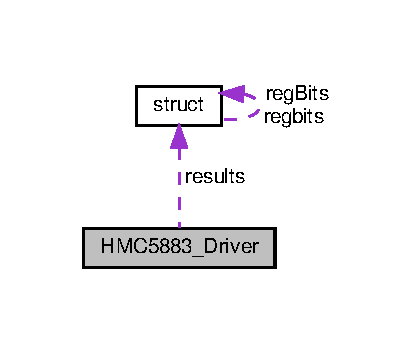
\includegraphics[width=199pt]{structHMC5883__Driver__coll__graph}
\end{center}
\end{figure}
\subsection*{Public Attributes}
\begin{DoxyCompactItemize}
\item 
\mbox{\Hypertarget{structHMC5883__Driver_a7e3b92c0b42e7121d70ef760c279beea}\label{structHMC5883__Driver_a7e3b92c0b42e7121d70ef760c279beea}} 
\hyperlink{vl53l0x__types_8h_aba7bc1797add20fe3efdf37ced1182c5}{uint8\+\_\+t} {\bfseries i2c\+\_\+bus}
\item 
\mbox{\Hypertarget{structHMC5883__Driver_aaf3b6257f1a9727ef32d9372e39a719c}\label{structHMC5883__Driver_aaf3b6257f1a9727ef32d9372e39a719c}} 
\hyperlink{vl53l0x__types_8h_aba7bc1797add20fe3efdf37ced1182c5}{uint8\+\_\+t} {\bfseries i2c\+\_\+address}
\item 
\mbox{\Hypertarget{structHMC5883__Driver_a2e8b3a8f9880e7ac56837c2cd35c80d9}\label{structHMC5883__Driver_a2e8b3a8f9880e7ac56837c2cd35c80d9}} 
bool {\bfseries isr\+\_\+en}
\item 
\mbox{\Hypertarget{structHMC5883__Driver_abc042870c5e7657aefb3cb3193618624}\label{structHMC5883__Driver_abc042870c5e7657aefb3cb3193618624}} 
bool {\bfseries isr\+\_\+pin\+\_\+configured}
\item 
\mbox{\Hypertarget{structHMC5883__Driver_a59f50a7e408988ed36204ca1767962db}\label{structHMC5883__Driver_a59f50a7e408988ed36204ca1767962db}} 
gpio\+\_\+num\+\_\+t {\bfseries drdy\+\_\+pin}
\item 
\mbox{\Hypertarget{structHMC5883__Driver_a79f78a6b7d768992b5052671527c8053}\label{structHMC5883__Driver_a79f78a6b7d768992b5052671527c8053}} 
hmc\+\_\+mode\+\_\+t {\bfseries mode}
\item 
\mbox{\Hypertarget{structHMC5883__Driver_a0d3b1d900f0a593095fa1f5096b6736b}\label{structHMC5883__Driver_a0d3b1d900f0a593095fa1f5096b6736b}} 
hmc\+\_\+scale\+\_\+t {\bfseries scale}
\item 
\mbox{\Hypertarget{structHMC5883__Driver_a9a1d32ee6489c6f49ee00b56050e8e4e}\label{structHMC5883__Driver_a9a1d32ee6489c6f49ee00b56050e8e4e}} 
hmc\+\_\+odr\+\_\+t {\bfseries d\+\_\+rate}
\item 
\mbox{\Hypertarget{structHMC5883__Driver_ae40e034b2260581e33fa590e3fd7afe1}\label{structHMC5883__Driver_ae40e034b2260581e33fa590e3fd7afe1}} 
hmc\+\_\+osr\+\_\+t {\bfseries osr}
\item 
\mbox{\Hypertarget{structHMC5883__Driver_a1134efbfe0ef26f01546dc7060de7440}\label{structHMC5883__Driver_a1134efbfe0ef26f01546dc7060de7440}} 
\hyperlink{structHMC__Measurements}{hmc\+\_\+measure\+\_\+t} {\bfseries results}
\item 
\mbox{\Hypertarget{structHMC5883__Driver_a3a69557b10567d5de073146c9293578b}\label{structHMC5883__Driver_a3a69557b10567d5de073146c9293578b}} 
Task\+Handle\+\_\+t {\bfseries t\+\_\+handle}
\end{DoxyCompactItemize}


The documentation for this struct was generated from the following file\+:\begin{DoxyCompactItemize}
\item 
H\+M\+C5885\+\_\+\+Driver/H\+M\+C5883\+\_\+\+Driver.\+h\end{DoxyCompactItemize}

\hypertarget{structHMC5883__init}{}\section{H\+M\+C5883\+\_\+init Struct Reference}
\label{structHMC5883__init}\index{H\+M\+C5883\+\_\+init@{H\+M\+C5883\+\_\+init}}
\subsection*{Public Attributes}
\begin{DoxyCompactItemize}
\item 
\mbox{\Hypertarget{structHMC5883__init_a8fcc55223034d87116e4a88416be05ab}\label{structHMC5883__init_a8fcc55223034d87116e4a88416be05ab}} 
\hyperlink{vl53l0x__types_8h_aba7bc1797add20fe3efdf37ced1182c5}{uint8\+\_\+t} {\bfseries i2c\+\_\+bus}
\item 
\mbox{\Hypertarget{structHMC5883__init_a8c9b48397e4df36740167f1c4e6e1e50}\label{structHMC5883__init_a8c9b48397e4df36740167f1c4e6e1e50}} 
gpio\+\_\+num\+\_\+t {\bfseries drdy\+\_\+pin}
\end{DoxyCompactItemize}


The documentation for this struct was generated from the following file\+:\begin{DoxyCompactItemize}
\item 
H\+M\+C5885\+\_\+\+Driver/H\+M\+C5883\+\_\+\+Driver.\+h\end{DoxyCompactItemize}

\hypertarget{structHMC__Measurements}{}\section{H\+M\+C\+\_\+\+Measurements Struct Reference}
\label{structHMC__Measurements}\index{H\+M\+C\+\_\+\+Measurements@{H\+M\+C\+\_\+\+Measurements}}
\subsection*{Public Attributes}
\begin{DoxyCompactItemize}
\item 
\mbox{\Hypertarget{structHMC__Measurements_abe88eba894640198dd401ebe064c38e4}\label{structHMC__Measurements_abe88eba894640198dd401ebe064c38e4}} 
float {\bfseries x\+\_\+val}
\item 
\mbox{\Hypertarget{structHMC__Measurements_a88015d635030cd43d90c8dd0a9f0cf4a}\label{structHMC__Measurements_a88015d635030cd43d90c8dd0a9f0cf4a}} 
float {\bfseries y\+\_\+val}
\item 
\mbox{\Hypertarget{structHMC__Measurements_a61ac0b342141e6a8cc2040171c2da7af}\label{structHMC__Measurements_a61ac0b342141e6a8cc2040171c2da7af}} 
float {\bfseries z\+\_\+val}
\item 
\mbox{\Hypertarget{structHMC__Measurements_a67f7afa8023b866bd67789e08b8f6c7a}\label{structHMC__Measurements_a67f7afa8023b866bd67789e08b8f6c7a}} 
\hyperlink{vl53l0x__types_8h_aa343fa3b3d06292b959ffdd4c4703b06}{int16\+\_\+t} {\bfseries x\+\_\+raw}
\item 
\mbox{\Hypertarget{structHMC__Measurements_ace80e715ae898ef5110f482a645652cf}\label{structHMC__Measurements_ace80e715ae898ef5110f482a645652cf}} 
\hyperlink{vl53l0x__types_8h_aa343fa3b3d06292b959ffdd4c4703b06}{int16\+\_\+t} {\bfseries y\+\_\+raw}
\item 
\mbox{\Hypertarget{structHMC__Measurements_a60511e3ca5bb79554f3f433e358e1dc1}\label{structHMC__Measurements_a60511e3ca5bb79554f3f433e358e1dc1}} 
\hyperlink{vl53l0x__types_8h_aa343fa3b3d06292b959ffdd4c4703b06}{int16\+\_\+t} {\bfseries z\+\_\+raw}
\end{DoxyCompactItemize}


The documentation for this struct was generated from the following file\+:\begin{DoxyCompactItemize}
\item 
H\+M\+C5885\+\_\+\+Driver/H\+M\+C5883\+\_\+\+Driver.\+h\end{DoxyCompactItemize}

\hypertarget{structHPDL1414__Driver}{}\section{H\+P\+D\+L1414\+\_\+\+Driver Struct Reference}
\label{structHPDL1414__Driver}\index{H\+P\+D\+L1414\+\_\+\+Driver@{H\+P\+D\+L1414\+\_\+\+Driver}}


Collaboration diagram for H\+P\+D\+L1414\+\_\+\+Driver\+:\nopagebreak
\begin{figure}[H]
\begin{center}
\leavevmode
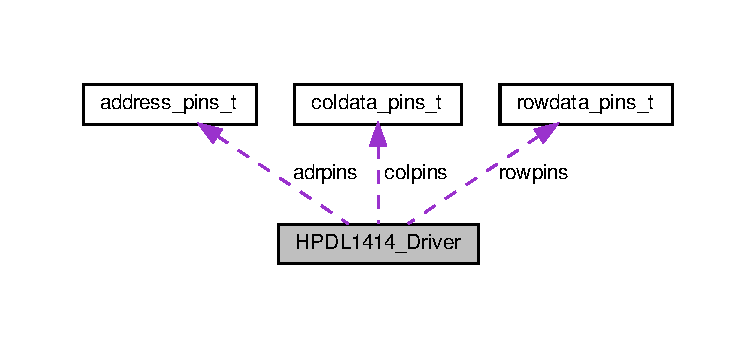
\includegraphics[width=350pt]{structHPDL1414__Driver__coll__graph}
\end{center}
\end{figure}
\subsection*{Public Attributes}
\begin{DoxyCompactItemize}
\item 
\mbox{\Hypertarget{structHPDL1414__Driver_a5524038b70f5bd39e288eb41e37c56a6}\label{structHPDL1414__Driver_a5524038b70f5bd39e288eb41e37c56a6}} 
\hyperlink{structrowdata__pins__t}{rowdata\+\_\+pins\+\_\+t} {\bfseries rowpins}
\item 
\mbox{\Hypertarget{structHPDL1414__Driver_acca32a90c225cf8ab271588f6cd35206}\label{structHPDL1414__Driver_acca32a90c225cf8ab271588f6cd35206}} 
\hyperlink{structcoldata__pins__t}{coldata\+\_\+pins\+\_\+t} {\bfseries colpins}
\item 
\mbox{\Hypertarget{structHPDL1414__Driver_ab048419e19192afc40fe92e918ee8f47}\label{structHPDL1414__Driver_ab048419e19192afc40fe92e918ee8f47}} 
\hyperlink{structaddress__pins__t}{address\+\_\+pins\+\_\+t} {\bfseries adrpins}
\item 
\mbox{\Hypertarget{structHPDL1414__Driver_ab3225ee4547f8fddba7acdc88117e873}\label{structHPDL1414__Driver_ab3225ee4547f8fddba7acdc88117e873}} 
gpio\+\_\+num\+\_\+t {\bfseries write\+\_\+pin}
\item 
\mbox{\Hypertarget{structHPDL1414__Driver_ae4ea4f16a3407a0126cf16b569dec815}\label{structHPDL1414__Driver_ae4ea4f16a3407a0126cf16b569dec815}} 
\hyperlink{vl53l0x__types_8h_aba7bc1797add20fe3efdf37ced1182c5}{uint8\+\_\+t} {\bfseries current\+\_\+led}
\end{DoxyCompactItemize}


The documentation for this struct was generated from the following file\+:\begin{DoxyCompactItemize}
\item 
H\+P\+D\+L1414\+\_\+\+Driver/H\+P\+D\+L1414\+\_\+\+Driver.\+h\end{DoxyCompactItemize}

\hypertarget{structHPDL1414__init}{}\section{H\+P\+D\+L1414\+\_\+init Struct Reference}
\label{structHPDL1414__init}\index{H\+P\+D\+L1414\+\_\+init@{H\+P\+D\+L1414\+\_\+init}}
\subsection*{Public Attributes}
\begin{DoxyCompactItemize}
\item 
\mbox{\Hypertarget{structHPDL1414__init_a2a6ecc27867895cfc9160162f7084586}\label{structHPDL1414__init_a2a6ecc27867895cfc9160162f7084586}} 
gpio\+\_\+num\+\_\+t {\bfseries D0}
\item 
\mbox{\Hypertarget{structHPDL1414__init_aa6747a659bf3ae45f0cabab8c9759722}\label{structHPDL1414__init_aa6747a659bf3ae45f0cabab8c9759722}} 
gpio\+\_\+num\+\_\+t {\bfseries D1}
\item 
\mbox{\Hypertarget{structHPDL1414__init_a1434f9dbc8d7f503d016d85e8a3b97d3}\label{structHPDL1414__init_a1434f9dbc8d7f503d016d85e8a3b97d3}} 
gpio\+\_\+num\+\_\+t {\bfseries D2}
\item 
\mbox{\Hypertarget{structHPDL1414__init_ac073d5bffb504176dfc99efbc328f821}\label{structHPDL1414__init_ac073d5bffb504176dfc99efbc328f821}} 
gpio\+\_\+num\+\_\+t {\bfseries D3}
\item 
\mbox{\Hypertarget{structHPDL1414__init_a37b836a1045674064991fd65359096a6}\label{structHPDL1414__init_a37b836a1045674064991fd65359096a6}} 
gpio\+\_\+num\+\_\+t {\bfseries D4}
\item 
\mbox{\Hypertarget{structHPDL1414__init_a85abdfaefe933b96d8e6fe7ebec55789}\label{structHPDL1414__init_a85abdfaefe933b96d8e6fe7ebec55789}} 
gpio\+\_\+num\+\_\+t {\bfseries D5}
\item 
\mbox{\Hypertarget{structHPDL1414__init_a0531fa643f6fe8c91bb5d95500d1898b}\label{structHPDL1414__init_a0531fa643f6fe8c91bb5d95500d1898b}} 
gpio\+\_\+num\+\_\+t {\bfseries D6}
\item 
\mbox{\Hypertarget{structHPDL1414__init_a7eb1aae8684305fc97a07dc83c8f7e6b}\label{structHPDL1414__init_a7eb1aae8684305fc97a07dc83c8f7e6b}} 
gpio\+\_\+num\+\_\+t {\bfseries A0}
\item 
\mbox{\Hypertarget{structHPDL1414__init_a18841e99a8598cf317ab25b2f38cf6b9}\label{structHPDL1414__init_a18841e99a8598cf317ab25b2f38cf6b9}} 
gpio\+\_\+num\+\_\+t {\bfseries A1}
\item 
\mbox{\Hypertarget{structHPDL1414__init_a9518004a4d3319a7a0eefe089e75a412}\label{structHPDL1414__init_a9518004a4d3319a7a0eefe089e75a412}} 
gpio\+\_\+num\+\_\+t {\bfseries write}
\end{DoxyCompactItemize}


The documentation for this struct was generated from the following file\+:\begin{DoxyCompactItemize}
\item 
H\+P\+D\+L1414\+\_\+\+Driver/H\+P\+D\+L1414\+\_\+\+Driver.\+h\end{DoxyCompactItemize}

\hypertarget{structledEffectData}{}\section{led\+Effect\+Data Struct Reference}
\label{structledEffectData}\index{led\+Effect\+Data@{led\+Effect\+Data}}


{\ttfamily \#include $<$Led\+Effects.\+h$>$}

\subsection*{Public Attributes}
\begin{DoxyCompactItemize}
\item 
\mbox{\Hypertarget{structledEffectData_a87074850f351bccf49dab4ff51f7d404}\label{structledEffectData_a87074850f351bccf49dab4ff51f7d404}} 
led\+Effect\+\_\+t {\bfseries effect}
\item 
Effect\+Function \hyperlink{structledEffectData_afda152477a636903c30cdb311e4d739b}{func}
\item 
\hyperlink{vl53l0x__types_8h_a435d1572bf3f880d55459d9805097f62}{uint32\+\_\+t} \hyperlink{structledEffectData_ab37d8733a0fc0c336752e382a53c2e6d}{colour}
\item 
\hyperlink{vl53l0x__types_8h_a273cf69d639a59973b6019625df33e30}{uint16\+\_\+t} \hyperlink{structledEffectData_af3091722f500797cff2896050b7ac3b4}{refresh\+\_\+t}
\item 
bool \hyperlink{structledEffectData_a5f73d846268058bf03c0cdea345ffa1b}{update\+Effect}
\item 
\hyperlink{vl53l0x__types_8h_aba7bc1797add20fe3efdf37ced1182c5}{uint8\+\_\+t} \hyperlink{structledEffectData_a8d68875aadb518d5292e93d79918d0ae}{brightness}
\item 
\hyperlink{vl53l0x__types_8h_a273cf69d639a59973b6019625df33e30}{uint16\+\_\+t} \hyperlink{structledEffectData_a980ab6cc1f7a667f35f5f56240dfd0e3}{var1}
\item 
\mbox{\Hypertarget{structledEffectData_a9a4ad08dc2c3ff67ae52e2f7544402ca}\label{structledEffectData_a9a4ad08dc2c3ff67ae52e2f7544402ca}} 
\hyperlink{vl53l0x__types_8h_a273cf69d639a59973b6019625df33e30}{uint16\+\_\+t} {\bfseries var2}
\item 
\mbox{\Hypertarget{structledEffectData_a0a9a8e27e0e818f4c57d5764a255ef0a}\label{structledEffectData_a0a9a8e27e0e818f4c57d5764a255ef0a}} 
\hyperlink{vl53l0x__types_8h_a435d1572bf3f880d55459d9805097f62}{uint32\+\_\+t} {\bfseries var3}
\item 
\mbox{\Hypertarget{structledEffectData_a64e20cccc9348363a0ba12bb5384ea78}\label{structledEffectData_a64e20cccc9348363a0ba12bb5384ea78}} 
\hyperlink{vl53l0x__types_8h_a435d1572bf3f880d55459d9805097f62}{uint32\+\_\+t} {\bfseries var4}
\item 
\mbox{\Hypertarget{structledEffectData_a94fe27a47d0b6946a95a21e3b4bac27b}\label{structledEffectData_a94fe27a47d0b6946a95a21e3b4bac27b}} 
bool {\bfseries var5}
\end{DoxyCompactItemize}


\subsection{Detailed Description}
Led effect struct Used for tracking persistent L\+ED effect variables? Try to build all effects to use the same type of data struct T\+O\+DO\+: better variable names, use union or bitfield? 

\subsection{Member Data Documentation}
\mbox{\Hypertarget{structledEffectData_a8d68875aadb518d5292e93d79918d0ae}\label{structledEffectData_a8d68875aadb518d5292e93d79918d0ae}} 
\index{led\+Effect\+Data@{led\+Effect\+Data}!brightness@{brightness}}
\index{brightness@{brightness}!led\+Effect\+Data@{led\+Effect\+Data}}
\subsubsection{\texorpdfstring{brightness}{brightness}}
{\footnotesize\ttfamily \hyperlink{vl53l0x__types_8h_aba7bc1797add20fe3efdf37ced1182c5}{uint8\+\_\+t} led\+Effect\+Data\+::brightness}

$<$ led effect has been changed -\/ adjust parameters \mbox{\Hypertarget{structledEffectData_ab37d8733a0fc0c336752e382a53c2e6d}\label{structledEffectData_ab37d8733a0fc0c336752e382a53c2e6d}} 
\index{led\+Effect\+Data@{led\+Effect\+Data}!colour@{colour}}
\index{colour@{colour}!led\+Effect\+Data@{led\+Effect\+Data}}
\subsubsection{\texorpdfstring{colour}{colour}}
{\footnotesize\ttfamily \hyperlink{vl53l0x__types_8h_a435d1572bf3f880d55459d9805097f62}{uint32\+\_\+t} led\+Effect\+Data\+::colour}

$<$ a pointer to the Led\+Effects function \mbox{\Hypertarget{structledEffectData_afda152477a636903c30cdb311e4d739b}\label{structledEffectData_afda152477a636903c30cdb311e4d739b}} 
\index{led\+Effect\+Data@{led\+Effect\+Data}!func@{func}}
\index{func@{func}!led\+Effect\+Data@{led\+Effect\+Data}}
\subsubsection{\texorpdfstring{func}{func}}
{\footnotesize\ttfamily Effect\+Function led\+Effect\+Data\+::func}

$<$ the current effect in enumeration \mbox{\Hypertarget{structledEffectData_af3091722f500797cff2896050b7ac3b4}\label{structledEffectData_af3091722f500797cff2896050b7ac3b4}} 
\index{led\+Effect\+Data@{led\+Effect\+Data}!refresh\+\_\+t@{refresh\+\_\+t}}
\index{refresh\+\_\+t@{refresh\+\_\+t}!led\+Effect\+Data@{led\+Effect\+Data}}
\subsubsection{\texorpdfstring{refresh\+\_\+t}{refresh\_t}}
{\footnotesize\ttfamily \hyperlink{vl53l0x__types_8h_a273cf69d639a59973b6019625df33e30}{uint16\+\_\+t} led\+Effect\+Data\+::refresh\+\_\+t}

$<$ colour -\/ colour \mbox{\Hypertarget{structledEffectData_a5f73d846268058bf03c0cdea345ffa1b}\label{structledEffectData_a5f73d846268058bf03c0cdea345ffa1b}} 
\index{led\+Effect\+Data@{led\+Effect\+Data}!update\+Effect@{update\+Effect}}
\index{update\+Effect@{update\+Effect}!led\+Effect\+Data@{led\+Effect\+Data}}
\subsubsection{\texorpdfstring{update\+Effect}{updateEffect}}
{\footnotesize\ttfamily bool led\+Effect\+Data\+::update\+Effect}

$<$ refresh time in ms -\/ 0 for no refresh \mbox{\Hypertarget{structledEffectData_a980ab6cc1f7a667f35f5f56240dfd0e3}\label{structledEffectData_a980ab6cc1f7a667f35f5f56240dfd0e3}} 
\index{led\+Effect\+Data@{led\+Effect\+Data}!var1@{var1}}
\index{var1@{var1}!led\+Effect\+Data@{led\+Effect\+Data}}
\subsubsection{\texorpdfstring{var1}{var1}}
{\footnotesize\ttfamily \hyperlink{vl53l0x__types_8h_a273cf69d639a59973b6019625df33e30}{uint16\+\_\+t} led\+Effect\+Data\+::var1}

$<$ led brigthness some variables for function use 

The documentation for this struct was generated from the following file\+:\begin{DoxyCompactItemize}
\item 
Utils/Led\+Effects.\+h\end{DoxyCompactItemize}

\hypertarget{structLSM__DeviceMeasures}{}\section{L\+S\+M\+\_\+\+Device\+Measures Struct Reference}
\label{structLSM__DeviceMeasures}\index{L\+S\+M\+\_\+\+Device\+Measures@{L\+S\+M\+\_\+\+Device\+Measures}}
\subsection*{Public Attributes}
\begin{DoxyCompactItemize}
\item 
\mbox{\Hypertarget{structLSM__DeviceMeasures_a4aaea68e518de41265b0a85f919125de}\label{structLSM__DeviceMeasures_a4aaea68e518de41265b0a85f919125de}} 
float {\bfseries calib\+GyroX}
\item 
float \hyperlink{structLSM__DeviceMeasures_a753796d24588a492de078e9257f7ca87}{calib\+GyroY}
\item 
\mbox{\Hypertarget{structLSM__DeviceMeasures_ac810ee16f2786fb40643d93b8a143057}\label{structLSM__DeviceMeasures_ac810ee16f2786fb40643d93b8a143057}} 
float {\bfseries calib\+GyroZ}
\item 
\mbox{\Hypertarget{structLSM__DeviceMeasures_a5cb3994dfd5b1c87bab20d79c695fea7}\label{structLSM__DeviceMeasures_a5cb3994dfd5b1c87bab20d79c695fea7}} 
float {\bfseries calib\+AccelX}
\item 
float \hyperlink{structLSM__DeviceMeasures_adcb5c49a650699c662f77f0b49b59a53}{calib\+AccelY}
\item 
float \hyperlink{structLSM__DeviceMeasures_a0d557711f5cae6f4216a394c4a2b2abd}{calib\+AccelZ}
\item 
\hyperlink{vl53l0x__types_8h_aba7bc1797add20fe3efdf37ced1182c5}{uint8\+\_\+t} \hyperlink{structLSM__DeviceMeasures_a9922b2bcf5d5a667712d6391757fb7d7}{raw\+Gyro} \mbox{[}6\mbox{]}
\item 
\mbox{\Hypertarget{structLSM__DeviceMeasures_a1d75674132b0a82a65f430a66b557f0b}\label{structLSM__DeviceMeasures_a1d75674132b0a82a65f430a66b557f0b}} 
\hyperlink{vl53l0x__types_8h_aba7bc1797add20fe3efdf37ced1182c5}{uint8\+\_\+t} {\bfseries raw\+Accel} \mbox{[}6\mbox{]}
\item 
\mbox{\Hypertarget{structLSM__DeviceMeasures_a7f02eddcdc48c2c362872e3b70e0a84a}\label{structLSM__DeviceMeasures_a7f02eddcdc48c2c362872e3b70e0a84a}} 
\hyperlink{vl53l0x__types_8h_aa343fa3b3d06292b959ffdd4c4703b06}{int16\+\_\+t} {\bfseries calib\+Temperature}
\item 
\mbox{\Hypertarget{structLSM__DeviceMeasures_a1a447dae80ad8d078657fc2d064dd942}\label{structLSM__DeviceMeasures_a1a447dae80ad8d078657fc2d064dd942}} 
\hyperlink{vl53l0x__types_8h_aba7bc1797add20fe3efdf37ced1182c5}{uint8\+\_\+t} {\bfseries raw\+\_\+temp} \mbox{[}2\mbox{]}
\end{DoxyCompactItemize}


\subsection{Member Data Documentation}
\mbox{\Hypertarget{structLSM__DeviceMeasures_adcb5c49a650699c662f77f0b49b59a53}\label{structLSM__DeviceMeasures_adcb5c49a650699c662f77f0b49b59a53}} 
\index{L\+S\+M\+\_\+\+Device\+Measures@{L\+S\+M\+\_\+\+Device\+Measures}!calib\+AccelY@{calib\+AccelY}}
\index{calib\+AccelY@{calib\+AccelY}!L\+S\+M\+\_\+\+Device\+Measures@{L\+S\+M\+\_\+\+Device\+Measures}}
\subsubsection{\texorpdfstring{calib\+AccelY}{calibAccelY}}
{\footnotesize\ttfamily float L\+S\+M\+\_\+\+Device\+Measures\+::calib\+AccelY}

$<$ in mG\textquotesingle{}s \mbox{\Hypertarget{structLSM__DeviceMeasures_a0d557711f5cae6f4216a394c4a2b2abd}\label{structLSM__DeviceMeasures_a0d557711f5cae6f4216a394c4a2b2abd}} 
\index{L\+S\+M\+\_\+\+Device\+Measures@{L\+S\+M\+\_\+\+Device\+Measures}!calib\+AccelZ@{calib\+AccelZ}}
\index{calib\+AccelZ@{calib\+AccelZ}!L\+S\+M\+\_\+\+Device\+Measures@{L\+S\+M\+\_\+\+Device\+Measures}}
\subsubsection{\texorpdfstring{calib\+AccelZ}{calibAccelZ}}
{\footnotesize\ttfamily float L\+S\+M\+\_\+\+Device\+Measures\+::calib\+AccelZ}

$<$ in mG\textquotesingle{}s \mbox{\Hypertarget{structLSM__DeviceMeasures_a753796d24588a492de078e9257f7ca87}\label{structLSM__DeviceMeasures_a753796d24588a492de078e9257f7ca87}} 
\index{L\+S\+M\+\_\+\+Device\+Measures@{L\+S\+M\+\_\+\+Device\+Measures}!calib\+GyroY@{calib\+GyroY}}
\index{calib\+GyroY@{calib\+GyroY}!L\+S\+M\+\_\+\+Device\+Measures@{L\+S\+M\+\_\+\+Device\+Measures}}
\subsubsection{\texorpdfstring{calib\+GyroY}{calibGyroY}}
{\footnotesize\ttfamily float L\+S\+M\+\_\+\+Device\+Measures\+::calib\+GyroY}

$<$ in m\+Degrees/s \mbox{\Hypertarget{structLSM__DeviceMeasures_a9922b2bcf5d5a667712d6391757fb7d7}\label{structLSM__DeviceMeasures_a9922b2bcf5d5a667712d6391757fb7d7}} 
\index{L\+S\+M\+\_\+\+Device\+Measures@{L\+S\+M\+\_\+\+Device\+Measures}!raw\+Gyro@{raw\+Gyro}}
\index{raw\+Gyro@{raw\+Gyro}!L\+S\+M\+\_\+\+Device\+Measures@{L\+S\+M\+\_\+\+Device\+Measures}}
\subsubsection{\texorpdfstring{raw\+Gyro}{rawGyro}}
{\footnotesize\ttfamily \hyperlink{vl53l0x__types_8h_aba7bc1797add20fe3efdf37ced1182c5}{uint8\+\_\+t} L\+S\+M\+\_\+\+Device\+Measures\+::raw\+Gyro\mbox{[}6\mbox{]}}

$<$ in mG\textquotesingle{}s 

The documentation for this struct was generated from the following file\+:\begin{DoxyCompactItemize}
\item 
L\+S\+M\+\_\+\+Driver/L\+S\+M\+\_\+\+Driver.\+h\end{DoxyCompactItemize}

\hypertarget{structLSM__deviceSettings}{}\section{L\+S\+M\+\_\+device\+Settings Struct Reference}
\label{structLSM__deviceSettings}\index{L\+S\+M\+\_\+device\+Settings@{L\+S\+M\+\_\+device\+Settings}}
\subsection*{Public Attributes}
\begin{DoxyCompactItemize}
\item 
\mbox{\Hypertarget{structLSM__deviceSettings_a31cb0f95054f6298e16f3a58e452e489}\label{structLSM__deviceSettings_a31cb0f95054f6298e16f3a58e452e489}} 
L\+S\+M\+\_\+\+Operating\+Mode\+\_\+t {\bfseries op\+Mode}
\item 
\mbox{\Hypertarget{structLSM__deviceSettings_ae2fbd1ba0dd7778e214f4c869ea05fd0}\label{structLSM__deviceSettings_ae2fbd1ba0dd7778e214f4c869ea05fd0}} 
L\+S\+M\+\_\+\+Highpass\+Slope\+Settings\+\_\+t {\bfseries high\+Pass}
\item 
\mbox{\Hypertarget{structLSM__deviceSettings_a4b02e8557e593c1ed00c6a4645d996ad}\label{structLSM__deviceSettings_a4b02e8557e593c1ed00c6a4645d996ad}} 
bool {\bfseries lowpass\+\_\+on\+\_\+6d\+\_\+en}
\item 
\mbox{\Hypertarget{structLSM__deviceSettings_ae7c3b8a96cf9e9af8e99168a1bd69a35}\label{structLSM__deviceSettings_ae7c3b8a96cf9e9af8e99168a1bd69a35}} 
bool {\bfseries embd\+\_\+functions\+\_\+en}
\item 
\mbox{\Hypertarget{structLSM__deviceSettings_a66a08d610b1f376fbb9876a38c47a550}\label{structLSM__deviceSettings_a66a08d610b1f376fbb9876a38c47a550}} 
L\+S\+M\+\_\+\+Accel\+Scale\+\_\+t {\bfseries accel\+Scale}
\item 
\mbox{\Hypertarget{structLSM__deviceSettings_a59afab5153af1c1a8ea8b668d2dee1ef}\label{structLSM__deviceSettings_a59afab5153af1c1a8ea8b668d2dee1ef}} 
L\+S\+M\+\_\+\+Accel\+O\+D\+R\+\_\+t {\bfseries accel\+Rate}
\item 
\mbox{\Hypertarget{structLSM__deviceSettings_a92232b1ed3e11b4440a15a9846436384}\label{structLSM__deviceSettings_a92232b1ed3e11b4440a15a9846436384}} 
L\+S\+M\+\_\+\+Accel\+Pwr\+Mode\+\_\+t {\bfseries accel\+Pwr}
\item 
L\+S\+M\+\_\+\+Accel\+Anti\+Alias\+B\+W\+\_\+t \hyperlink{structLSM__deviceSettings_ae9bfe4e1b72fde4f37df849563092908}{accel\+AA}
\item 
\mbox{\Hypertarget{structLSM__deviceSettings_a741ec948e81621aa2fc6d839f3f1f1b9}\label{structLSM__deviceSettings_a741ec948e81621aa2fc6d839f3f1f1b9}} 
L\+S\+M\+\_\+\+Fifo\+Pkt\+Cfg\+\_\+t {\bfseries accel\+Dec}
\item 
\mbox{\Hypertarget{structLSM__deviceSettings_a3ec9e5e5b14a2d56209ea078b1debbcc}\label{structLSM__deviceSettings_a3ec9e5e5b14a2d56209ea078b1debbcc}} 
bool {\bfseries accel\+\_\+lp2\+\_\+filter\+\_\+en}
\item 
\mbox{\Hypertarget{structLSM__deviceSettings_a38bc059241e8e65f1f442b60d26e3fe5}\label{structLSM__deviceSettings_a38bc059241e8e65f1f442b60d26e3fe5}} 
bool {\bfseries accel\+\_\+hp\+\_\+filter\+\_\+en}
\item 
\mbox{\Hypertarget{structLSM__deviceSettings_ae4a134c3382b1057d0eff5d517054556}\label{structLSM__deviceSettings_ae4a134c3382b1057d0eff5d517054556}} 
L\+S\+M\+\_\+\+Gyro\+Scale\+\_\+t {\bfseries gyro\+Scale}
\item 
\mbox{\Hypertarget{structLSM__deviceSettings_ad57c22fbaae21fd6be08545c1501c8bf}\label{structLSM__deviceSettings_ad57c22fbaae21fd6be08545c1501c8bf}} 
L\+S\+M\+\_\+\+Gyro\+O\+D\+R\+\_\+t {\bfseries gyro\+Rate}
\item 
\mbox{\Hypertarget{structLSM__deviceSettings_aa08e433ba639467a101261c93fc897a3}\label{structLSM__deviceSettings_aa08e433ba639467a101261c93fc897a3}} 
L\+S\+M\+\_\+\+Gyro\+Pwr\+Mode\+\_\+t {\bfseries gyro\+Pwr}
\item 
bool \hyperlink{structLSM__deviceSettings_a86ae7e0b0ec3cc7aa48308c788062522}{gyro\+\_\+hp\+\_\+en}
\item 
\mbox{\Hypertarget{structLSM__deviceSettings_a3f7f8ef24eaa04ef0301c80af5a363bc}\label{structLSM__deviceSettings_a3f7f8ef24eaa04ef0301c80af5a363bc}} 
bool {\bfseries gyro\+\_\+hp\+\_\+filter\+\_\+en}
\item 
\mbox{\Hypertarget{structLSM__deviceSettings_a5f133f1bc76c2ac0762713c8b185b292}\label{structLSM__deviceSettings_a5f133f1bc76c2ac0762713c8b185b292}} 
L\+S\+M\+\_\+\+Gyro\+Highpass\+Cutoff\+\_\+t {\bfseries G\+H\+Pcutoff}
\item 
\mbox{\Hypertarget{structLSM__deviceSettings_ae2f9f08a9135f4abe820deda7abe2d70}\label{structLSM__deviceSettings_ae2f9f08a9135f4abe820deda7abe2d70}} 
L\+S\+M\+\_\+\+Fifo\+Pkt\+Cfg\+\_\+t {\bfseries gyro\+Dec}
\item 
\mbox{\Hypertarget{structLSM__deviceSettings_aded1b560f71f5fee81639674914d331c}\label{structLSM__deviceSettings_aded1b560f71f5fee81639674914d331c}} 
\hyperlink{vl53l0x__types_8h_aba7bc1797add20fe3efdf37ced1182c5}{uint8\+\_\+t} {\bfseries int1\+\_\+mask}
\item 
\mbox{\Hypertarget{structLSM__deviceSettings_ac9dc18bfdb0e9951cbfe338ffeda701c}\label{structLSM__deviceSettings_ac9dc18bfdb0e9951cbfe338ffeda701c}} 
\hyperlink{vl53l0x__types_8h_aba7bc1797add20fe3efdf37ced1182c5}{uint8\+\_\+t} {\bfseries int2\+\_\+mask}
\item 
\mbox{\Hypertarget{structLSM__deviceSettings_a381c2d5d81b7cb10c5861d42e2f0e446}\label{structLSM__deviceSettings_a381c2d5d81b7cb10c5861d42e2f0e446}} 
\hyperlink{vl53l0x__types_8h_aba7bc1797add20fe3efdf37ced1182c5}{uint8\+\_\+t} {\bfseries int2\+\_\+on\+\_\+int1}
\item 
\mbox{\Hypertarget{structLSM__deviceSettings_aaf6634f33453f03cb21463147cebc18b}\label{structLSM__deviceSettings_aaf6634f33453f03cb21463147cebc18b}} 
L\+S\+M\+\_\+\+F\+I\+F\+O\+Mode\+\_\+t {\bfseries fifo\+Mode}
\item 
\mbox{\Hypertarget{structLSM__deviceSettings_ad8c7f6a1ac4146514593f9f6c80adc52}\label{structLSM__deviceSettings_ad8c7f6a1ac4146514593f9f6c80adc52}} 
L\+S\+M\+\_\+\+F\+I\+F\+Oodr\+\_\+t {\bfseries fifo\+O\+DR}
\item 
\mbox{\Hypertarget{structLSM__deviceSettings_a554156bf39e90867d2db5bf416ba52b4}\label{structLSM__deviceSettings_a554156bf39e90867d2db5bf416ba52b4}} 
\hyperlink{vl53l0x__types_8h_a273cf69d639a59973b6019625df33e30}{uint16\+\_\+t} {\bfseries watermark}
\item 
\mbox{\Hypertarget{structLSM__deviceSettings_a2dc01f5e521410267b13f2859ee85d6b}\label{structLSM__deviceSettings_a2dc01f5e521410267b13f2859ee85d6b}} 
bool {\bfseries stop\+\_\+on\+\_\+thresh}
\item 
\mbox{\Hypertarget{structLSM__deviceSettings_a0b6bca1c049d76dc755060399b4ebbab}\label{structLSM__deviceSettings_a0b6bca1c049d76dc755060399b4ebbab}} 
\hyperlink{vl53l0x__types_8h_aba7bc1797add20fe3efdf37ced1182c5}{uint8\+\_\+t} {\bfseries fifo\+Pkt\+Len}
\item 
\mbox{\Hypertarget{structLSM__deviceSettings_aac81e196c5abb1adf2106da9b857d5fa}\label{structLSM__deviceSettings_aac81e196c5abb1adf2106da9b857d5fa}} 
bool {\bfseries pedo\+\_\+fifo\+\_\+en}
\item 
\mbox{\Hypertarget{structLSM__deviceSettings_ade90067d6ed8b1c04d8b8a5f5bb9f966}\label{structLSM__deviceSettings_ade90067d6ed8b1c04d8b8a5f5bb9f966}} 
L\+S\+M\+\_\+\+Fifo\+Pkt\+Cfg\+\_\+t {\bfseries step\+Dec}
\item 
\mbox{\Hypertarget{structLSM__deviceSettings_a9a9ebe7a73b3d81f7892084a5403c8cb}\label{structLSM__deviceSettings_a9a9ebe7a73b3d81f7892084a5403c8cb}} 
bool {\bfseries msb\+\_\+only\+\_\+en}
\item 
\mbox{\Hypertarget{structLSM__deviceSettings_a8c1826cbc8a9207ba1d0676bf300e47f}\label{structLSM__deviceSettings_a8c1826cbc8a9207ba1d0676bf300e47f}} 
\hyperlink{vl53l0x__types_8h_aba7bc1797add20fe3efdf37ced1182c5}{uint8\+\_\+t} {\bfseries step\+\_\+drdy\+\_\+en}
\item 
\mbox{\Hypertarget{structLSM__deviceSettings_a538b1478215503499fa6c90f4622eb0e}\label{structLSM__deviceSettings_a538b1478215503499fa6c90f4622eb0e}} 
bool {\bfseries temp\+\_\+pkt\+\_\+en}
\item 
\mbox{\Hypertarget{structLSM__deviceSettings_a5d42118b6dba521f58cbc91dbaa100b5}\label{structLSM__deviceSettings_a5d42118b6dba521f58cbc91dbaa100b5}} 
bool {\bfseries block\+\_\+data\+\_\+update}
\item 
\mbox{\Hypertarget{structLSM__deviceSettings_a331cd41bef375aba42566805cc1488bc}\label{structLSM__deviceSettings_a331cd41bef375aba42566805cc1488bc}} 
L\+S\+M\+\_\+\+Accel\+Bandwidth\+Mode\+\_\+t {\bfseries accel\+\_\+bw\+\_\+mode}
\item 
\mbox{\Hypertarget{structLSM__deviceSettings_a799f004d5fd6341d393e739c7e82c344}\label{structLSM__deviceSettings_a799f004d5fd6341d393e739c7e82c344}} 
L\+S\+M\+\_\+\+Gyro\+Sleep\+State\+\_\+t {\bfseries gyro\+\_\+sleep\+\_\+state}
\end{DoxyCompactItemize}


\subsection{Member Data Documentation}
\mbox{\Hypertarget{structLSM__deviceSettings_ae9bfe4e1b72fde4f37df849563092908}\label{structLSM__deviceSettings_ae9bfe4e1b72fde4f37df849563092908}} 
\index{L\+S\+M\+\_\+device\+Settings@{L\+S\+M\+\_\+device\+Settings}!accel\+AA@{accel\+AA}}
\index{accel\+AA@{accel\+AA}!L\+S\+M\+\_\+device\+Settings@{L\+S\+M\+\_\+device\+Settings}}
\subsubsection{\texorpdfstring{accel\+AA}{accelAA}}
{\footnotesize\ttfamily L\+S\+M\+\_\+\+Accel\+Anti\+Alias\+B\+W\+\_\+t L\+S\+M\+\_\+device\+Settings\+::accel\+AA}

obsolete? \mbox{\Hypertarget{structLSM__deviceSettings_a86ae7e0b0ec3cc7aa48308c788062522}\label{structLSM__deviceSettings_a86ae7e0b0ec3cc7aa48308c788062522}} 
\index{L\+S\+M\+\_\+device\+Settings@{L\+S\+M\+\_\+device\+Settings}!gyro\+\_\+hp\+\_\+en@{gyro\+\_\+hp\+\_\+en}}
\index{gyro\+\_\+hp\+\_\+en@{gyro\+\_\+hp\+\_\+en}!L\+S\+M\+\_\+device\+Settings@{L\+S\+M\+\_\+device\+Settings}}
\subsubsection{\texorpdfstring{gyro\+\_\+hp\+\_\+en}{gyro\_hp\_en}}
{\footnotesize\ttfamily bool L\+S\+M\+\_\+device\+Settings\+::gyro\+\_\+hp\+\_\+en}

obsolete ? 

The documentation for this struct was generated from the following file\+:\begin{DoxyCompactItemize}
\item 
L\+S\+M\+\_\+\+Driver/L\+S\+M\+\_\+\+Driver.\+h\end{DoxyCompactItemize}

\hypertarget{structLSM__Driver__settings}{}\section{L\+S\+M\+\_\+\+Driver\+\_\+settings Struct Reference}
\label{structLSM__Driver__settings}\index{L\+S\+M\+\_\+\+Driver\+\_\+settings@{L\+S\+M\+\_\+\+Driver\+\_\+settings}}
\subsection*{Public Attributes}
\begin{DoxyCompactItemize}
\item 
\mbox{\Hypertarget{structLSM__Driver__settings_a2660432eceddfb51dd84845092fb5cf3}\label{structLSM__Driver__settings_a2660432eceddfb51dd84845092fb5cf3}} 
bool {\bfseries auto\+\_\+read\+\_\+fifo\+\_\+full}
\item 
\mbox{\Hypertarget{structLSM__Driver__settings_aa6a9de82faf20e36929c683c85772b54}\label{structLSM__Driver__settings_aa6a9de82faf20e36929c683c85772b54}} 
bool {\bfseries auto\+\_\+read\+\_\+sample\+\_\+rdy}
\item 
\mbox{\Hypertarget{structLSM__Driver__settings_afa2d22be287b87b0e04c5e793616e6e2}\label{structLSM__Driver__settings_afa2d22be287b87b0e04c5e793616e6e2}} 
bool {\bfseries poll\+\_\+sample\+\_\+ready}
\item 
\mbox{\Hypertarget{structLSM__Driver__settings_ae4efa962818a2507a11947178837b6f2}\label{structLSM__Driver__settings_ae4efa962818a2507a11947178837b6f2}} 
\hyperlink{vl53l0x__types_8h_a273cf69d639a59973b6019625df33e30}{uint16\+\_\+t} {\bfseries sample\+\_\+poll\+\_\+ms}
\end{DoxyCompactItemize}


The documentation for this struct was generated from the following file\+:\begin{DoxyCompactItemize}
\item 
L\+S\+M\+\_\+\+Driver/L\+S\+M\+\_\+\+Driver.\+h\end{DoxyCompactItemize}

\hypertarget{structLSM__DriverSettings}{}\section{L\+S\+M\+\_\+\+Driver\+Settings Struct Reference}
\label{structLSM__DriverSettings}\index{L\+S\+M\+\_\+\+Driver\+Settings@{L\+S\+M\+\_\+\+Driver\+Settings}}


{\ttfamily \#include $<$L\+S\+M\+\_\+\+Driver.\+h$>$}



Collaboration diagram for L\+S\+M\+\_\+\+Driver\+Settings\+:\nopagebreak
\begin{figure}[H]
\begin{center}
\leavevmode
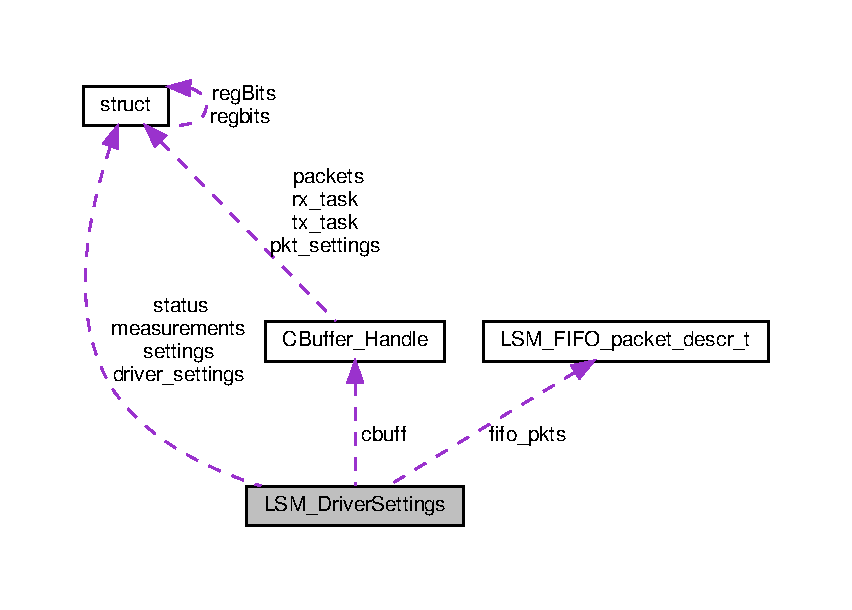
\includegraphics[width=350pt]{structLSM__DriverSettings__coll__graph}
\end{center}
\end{figure}
\subsection*{Public Attributes}
\begin{DoxyCompactItemize}
\item 
\mbox{\Hypertarget{structLSM__DriverSettings_abe7b9a8eb65e5c787bb575c20eb632fb}\label{structLSM__DriverSettings_abe7b9a8eb65e5c787bb575c20eb632fb}} 
\hyperlink{vl53l0x__types_8h_a273cf69d639a59973b6019625df33e30}{uint16\+\_\+t} {\bfseries i1\+Pin}
\item 
\hyperlink{vl53l0x__types_8h_a273cf69d639a59973b6019625df33e30}{uint16\+\_\+t} \hyperlink{structLSM__DriverSettings_ac5e7d16098a2edade5754f2eba5d4b6e}{i2\+Pin}
\item 
bool \hyperlink{structLSM__DriverSettings_a1909b0fde3f2597bfff85f710155fa5a}{int1\+En}
\item 
bool \hyperlink{structLSM__DriverSettings_aeb418668f399649751cd76daf50e9f5b}{int2\+En}
\item 
\hyperlink{vl53l0x__types_8h_aba7bc1797add20fe3efdf37ced1182c5}{uint8\+\_\+t} \hyperlink{structLSM__DriverSettings_a70745c29bbb1a152fd864788bf442d90}{intr1\+\_\+mask}
\item 
\hyperlink{vl53l0x__types_8h_aba7bc1797add20fe3efdf37ced1182c5}{uint8\+\_\+t} \hyperlink{structLSM__DriverSettings_a1e63a45c4aa7308f24ae90cb12027383}{intr2\+\_\+mask}
\item 
L\+S\+M\+\_\+\+Device\+Comm\+Mode\+\_\+t \hyperlink{structLSM__DriverSettings_a2931e2571bc690535ac6d2c1730f52d6}{comm\+Mode}
\item 
\hyperlink{structLSM__deviceSettings}{L\+S\+M\+\_\+\+Device\+Settings\+\_\+t} \hyperlink{structLSM__DriverSettings_aa13696d3b69d61affa5f8ece697da108}{settings}
\item 
\hyperlink{structLSM__DeviceMeasures}{L\+S\+M\+\_\+\+Device\+Measures\+\_\+t} \hyperlink{structLSM__DriverSettings_a17dd42c3eba587838df128376bfa834f}{measurements}
\item 
\hyperlink{structLSM__Driver__settings}{L\+S\+M\+\_\+\+Driver\+\_\+settings\+\_\+t} \hyperlink{structLSM__DriverSettings_a27fddf0bb2b33710460e4df455461054}{driver\+\_\+settings}
\item 
\hyperlink{structLSM__FIFO__packet__descr__t}{L\+S\+M\+\_\+\+F\+I\+F\+O\+\_\+packet\+\_\+descr\+\_\+t} \hyperlink{structLSM__DriverSettings_a3f5bf280c1d267d58e45bd8ac2d06040}{fifo\+\_\+pkts}
\item 
\hyperlink{structLSM__status}{L\+S\+M\+\_\+status\+\_\+t} \hyperlink{structLSM__DriverSettings_a75f33ebc368b5b1f3b0651cb16f4105c}{status}
\item 
\hyperlink{vl53l0x__types_8h_aba7bc1797add20fe3efdf37ced1182c5}{uint8\+\_\+t} \hyperlink{structLSM__DriverSettings_add57a764f16d59e082ddb79bc7c74180}{comms\+Channel}
\item 
\hyperlink{vl53l0x__types_8h_aba7bc1797add20fe3efdf37ced1182c5}{uint8\+\_\+t} \hyperlink{structLSM__DriverSettings_a8e1a6b136f50016aaab1ae491a751336}{dev\+Addr}
\item 
\hyperlink{vl53l0x__types_8h_aba7bc1797add20fe3efdf37ced1182c5}{uint8\+\_\+t} \hyperlink{structLSM__DriverSettings_a2d20232c5ac5d8eb5190ea9e67a80520}{comms\+Handle}
\item 
void $\ast$ \hyperlink{structLSM__DriverSettings_afadd6b60a58629b31e48a5f8b4903d8e}{fifo\+Buffer}
\item 
bool \hyperlink{structLSM__DriverSettings_a9ac1f71e45d64c08137e4a66ceb037b6}{use\+\_\+cbuffer}
\item 
bool \hyperlink{structLSM__DriverSettings_a16df6adafa33bd8989b4c8dc4bb35cfc}{cbuff\+\_\+store\+\_\+packets}
\item 
bool \hyperlink{structLSM__DriverSettings_ac9afe83a3868f908a254f4b899fbf545}{cbuff\+\_\+store\+\_\+raw}
\item 
\hyperlink{structCBuffer__Handle}{C\+Buff} \hyperlink{structLSM__DriverSettings_a40dcf1c51a0b4d0725ac4ddde56afcf3}{cbuff}
\item 
bool \hyperlink{structLSM__DriverSettings_ab816e595f9f91a9a5887e806d62458b0}{use\+\_\+events}
\item 
\hyperlink{vl53l0x__types_8h_aba7bc1797add20fe3efdf37ced1182c5}{uint8\+\_\+t} \hyperlink{structLSM__DriverSettings_a97c8a07da0167f7022bcff555ec28b9c}{event\+\_\+mask}
\item 
esp\+\_\+event\+\_\+loop\+\_\+handle\+\_\+t \hyperlink{structLSM__DriverSettings_a88424f1e21f40ed7c4eac94eb449c051}{loop}
\item 
\mbox{\Hypertarget{structLSM__DriverSettings_a30d4b8a2c3eb2682503e8f38eb08257d}\label{structLSM__DriverSettings_a30d4b8a2c3eb2682503e8f38eb08257d}} 
Task\+Handle\+\_\+t {\bfseries task\+Handle}
\end{DoxyCompactItemize}


\subsection{Detailed Description}
L\+S\+M\+\_\+\+Driver\+Handle\+\_\+t -\/ a settings struct for the device keep track of various things.. 

\subsection{Member Data Documentation}
\mbox{\Hypertarget{structLSM__DriverSettings_a40dcf1c51a0b4d0725ac4ddde56afcf3}\label{structLSM__DriverSettings_a40dcf1c51a0b4d0725ac4ddde56afcf3}} 
\index{L\+S\+M\+\_\+\+Driver\+Settings@{L\+S\+M\+\_\+\+Driver\+Settings}!cbuff@{cbuff}}
\index{cbuff@{cbuff}!L\+S\+M\+\_\+\+Driver\+Settings@{L\+S\+M\+\_\+\+Driver\+Settings}}
\subsubsection{\texorpdfstring{cbuff}{cbuff}}
{\footnotesize\ttfamily \hyperlink{structCBuffer__Handle}{C\+Buff} L\+S\+M\+\_\+\+Driver\+Settings\+::cbuff}

cbuffer handle, N\+U\+LL if unused \mbox{\Hypertarget{structLSM__DriverSettings_a16df6adafa33bd8989b4c8dc4bb35cfc}\label{structLSM__DriverSettings_a16df6adafa33bd8989b4c8dc4bb35cfc}} 
\index{L\+S\+M\+\_\+\+Driver\+Settings@{L\+S\+M\+\_\+\+Driver\+Settings}!cbuff\+\_\+store\+\_\+packets@{cbuff\+\_\+store\+\_\+packets}}
\index{cbuff\+\_\+store\+\_\+packets@{cbuff\+\_\+store\+\_\+packets}!L\+S\+M\+\_\+\+Driver\+Settings@{L\+S\+M\+\_\+\+Driver\+Settings}}
\subsubsection{\texorpdfstring{cbuff\+\_\+store\+\_\+packets}{cbuff\_store\_packets}}
{\footnotesize\ttfamily bool L\+S\+M\+\_\+\+Driver\+Settings\+::cbuff\+\_\+store\+\_\+packets}

store fifo data packets as cbuffer packets -\/ formats should match! \mbox{\Hypertarget{structLSM__DriverSettings_ac9afe83a3868f908a254f4b899fbf545}\label{structLSM__DriverSettings_ac9afe83a3868f908a254f4b899fbf545}} 
\index{L\+S\+M\+\_\+\+Driver\+Settings@{L\+S\+M\+\_\+\+Driver\+Settings}!cbuff\+\_\+store\+\_\+raw@{cbuff\+\_\+store\+\_\+raw}}
\index{cbuff\+\_\+store\+\_\+raw@{cbuff\+\_\+store\+\_\+raw}!L\+S\+M\+\_\+\+Driver\+Settings@{L\+S\+M\+\_\+\+Driver\+Settings}}
\subsubsection{\texorpdfstring{cbuff\+\_\+store\+\_\+raw}{cbuff\_store\_raw}}
{\footnotesize\ttfamily bool L\+S\+M\+\_\+\+Driver\+Settings\+::cbuff\+\_\+store\+\_\+raw}

if true, store the raw integers, else store converted \mbox{\Hypertarget{structLSM__DriverSettings_a2931e2571bc690535ac6d2c1730f52d6}\label{structLSM__DriverSettings_a2931e2571bc690535ac6d2c1730f52d6}} 
\index{L\+S\+M\+\_\+\+Driver\+Settings@{L\+S\+M\+\_\+\+Driver\+Settings}!comm\+Mode@{comm\+Mode}}
\index{comm\+Mode@{comm\+Mode}!L\+S\+M\+\_\+\+Driver\+Settings@{L\+S\+M\+\_\+\+Driver\+Settings}}
\subsubsection{\texorpdfstring{comm\+Mode}{commMode}}
{\footnotesize\ttfamily L\+S\+M\+\_\+\+Device\+Comm\+Mode\+\_\+t L\+S\+M\+\_\+\+Driver\+Settings\+::comm\+Mode}

$<$ interrupt enabled on intr 2 \mbox{\Hypertarget{structLSM__DriverSettings_add57a764f16d59e082ddb79bc7c74180}\label{structLSM__DriverSettings_add57a764f16d59e082ddb79bc7c74180}} 
\index{L\+S\+M\+\_\+\+Driver\+Settings@{L\+S\+M\+\_\+\+Driver\+Settings}!comms\+Channel@{comms\+Channel}}
\index{comms\+Channel@{comms\+Channel}!L\+S\+M\+\_\+\+Driver\+Settings@{L\+S\+M\+\_\+\+Driver\+Settings}}
\subsubsection{\texorpdfstring{comms\+Channel}{commsChannel}}
{\footnotesize\ttfamily \hyperlink{vl53l0x__types_8h_aba7bc1797add20fe3efdf37ced1182c5}{uint8\+\_\+t} L\+S\+M\+\_\+\+Driver\+Settings\+::comms\+Channel}

comms settings \mbox{\Hypertarget{structLSM__DriverSettings_a2d20232c5ac5d8eb5190ea9e67a80520}\label{structLSM__DriverSettings_a2d20232c5ac5d8eb5190ea9e67a80520}} 
\index{L\+S\+M\+\_\+\+Driver\+Settings@{L\+S\+M\+\_\+\+Driver\+Settings}!comms\+Handle@{comms\+Handle}}
\index{comms\+Handle@{comms\+Handle}!L\+S\+M\+\_\+\+Driver\+Settings@{L\+S\+M\+\_\+\+Driver\+Settings}}
\subsubsection{\texorpdfstring{comms\+Handle}{commsHandle}}
{\footnotesize\ttfamily \hyperlink{vl53l0x__types_8h_aba7bc1797add20fe3efdf37ced1182c5}{uint8\+\_\+t} L\+S\+M\+\_\+\+Driver\+Settings\+::comms\+Handle}

$<$ the device i2c address \mbox{\Hypertarget{structLSM__DriverSettings_a8e1a6b136f50016aaab1ae491a751336}\label{structLSM__DriverSettings_a8e1a6b136f50016aaab1ae491a751336}} 
\index{L\+S\+M\+\_\+\+Driver\+Settings@{L\+S\+M\+\_\+\+Driver\+Settings}!dev\+Addr@{dev\+Addr}}
\index{dev\+Addr@{dev\+Addr}!L\+S\+M\+\_\+\+Driver\+Settings@{L\+S\+M\+\_\+\+Driver\+Settings}}
\subsubsection{\texorpdfstring{dev\+Addr}{devAddr}}
{\footnotesize\ttfamily \hyperlink{vl53l0x__types_8h_aba7bc1797add20fe3efdf37ced1182c5}{uint8\+\_\+t} L\+S\+M\+\_\+\+Driver\+Settings\+::dev\+Addr}

$<$ the i2c or spi channel being used \mbox{\Hypertarget{structLSM__DriverSettings_a27fddf0bb2b33710460e4df455461054}\label{structLSM__DriverSettings_a27fddf0bb2b33710460e4df455461054}} 
\index{L\+S\+M\+\_\+\+Driver\+Settings@{L\+S\+M\+\_\+\+Driver\+Settings}!driver\+\_\+settings@{driver\+\_\+settings}}
\index{driver\+\_\+settings@{driver\+\_\+settings}!L\+S\+M\+\_\+\+Driver\+Settings@{L\+S\+M\+\_\+\+Driver\+Settings}}
\subsubsection{\texorpdfstring{driver\+\_\+settings}{driver\_settings}}
{\footnotesize\ttfamily \hyperlink{structLSM__Driver__settings}{L\+S\+M\+\_\+\+Driver\+\_\+settings\+\_\+t} L\+S\+M\+\_\+\+Driver\+Settings\+::driver\+\_\+settings}

$<$ the device\textquotesingle{}s latest measurtements settings for the driver \mbox{\Hypertarget{structLSM__DriverSettings_a97c8a07da0167f7022bcff555ec28b9c}\label{structLSM__DriverSettings_a97c8a07da0167f7022bcff555ec28b9c}} 
\index{L\+S\+M\+\_\+\+Driver\+Settings@{L\+S\+M\+\_\+\+Driver\+Settings}!event\+\_\+mask@{event\+\_\+mask}}
\index{event\+\_\+mask@{event\+\_\+mask}!L\+S\+M\+\_\+\+Driver\+Settings@{L\+S\+M\+\_\+\+Driver\+Settings}}
\subsubsection{\texorpdfstring{event\+\_\+mask}{event\_mask}}
{\footnotesize\ttfamily \hyperlink{vl53l0x__types_8h_aba7bc1797add20fe3efdf37ced1182c5}{uint8\+\_\+t} L\+S\+M\+\_\+\+Driver\+Settings\+::event\+\_\+mask}

event mask bits -\/ OR\textquotesingle{}d byte of event bits above \mbox{\Hypertarget{structLSM__DriverSettings_a3f5bf280c1d267d58e45bd8ac2d06040}\label{structLSM__DriverSettings_a3f5bf280c1d267d58e45bd8ac2d06040}} 
\index{L\+S\+M\+\_\+\+Driver\+Settings@{L\+S\+M\+\_\+\+Driver\+Settings}!fifo\+\_\+pkts@{fifo\+\_\+pkts}}
\index{fifo\+\_\+pkts@{fifo\+\_\+pkts}!L\+S\+M\+\_\+\+Driver\+Settings@{L\+S\+M\+\_\+\+Driver\+Settings}}
\subsubsection{\texorpdfstring{fifo\+\_\+pkts}{fifo\_pkts}}
{\footnotesize\ttfamily \hyperlink{structLSM__FIFO__packet__descr__t}{L\+S\+M\+\_\+\+F\+I\+F\+O\+\_\+packet\+\_\+descr\+\_\+t} L\+S\+M\+\_\+\+Driver\+Settings\+::fifo\+\_\+pkts}

description of fifo packets \mbox{\Hypertarget{structLSM__DriverSettings_afadd6b60a58629b31e48a5f8b4903d8e}\label{structLSM__DriverSettings_afadd6b60a58629b31e48a5f8b4903d8e}} 
\index{L\+S\+M\+\_\+\+Driver\+Settings@{L\+S\+M\+\_\+\+Driver\+Settings}!fifo\+Buffer@{fifo\+Buffer}}
\index{fifo\+Buffer@{fifo\+Buffer}!L\+S\+M\+\_\+\+Driver\+Settings@{L\+S\+M\+\_\+\+Driver\+Settings}}
\subsubsection{\texorpdfstring{fifo\+Buffer}{fifoBuffer}}
{\footnotesize\ttfamily void$\ast$ L\+S\+M\+\_\+\+Driver\+Settings\+::fifo\+Buffer}

$<$ can be used to hold a device handle \mbox{\Hypertarget{structLSM__DriverSettings_ac5e7d16098a2edade5754f2eba5d4b6e}\label{structLSM__DriverSettings_ac5e7d16098a2edade5754f2eba5d4b6e}} 
\index{L\+S\+M\+\_\+\+Driver\+Settings@{L\+S\+M\+\_\+\+Driver\+Settings}!i2\+Pin@{i2\+Pin}}
\index{i2\+Pin@{i2\+Pin}!L\+S\+M\+\_\+\+Driver\+Settings@{L\+S\+M\+\_\+\+Driver\+Settings}}
\subsubsection{\texorpdfstring{i2\+Pin}{i2Pin}}
{\footnotesize\ttfamily \hyperlink{vl53l0x__types_8h_a273cf69d639a59973b6019625df33e30}{uint16\+\_\+t} L\+S\+M\+\_\+\+Driver\+Settings\+::i2\+Pin}

$<$ gpio interrupt pin 1 \mbox{\Hypertarget{structLSM__DriverSettings_a1909b0fde3f2597bfff85f710155fa5a}\label{structLSM__DriverSettings_a1909b0fde3f2597bfff85f710155fa5a}} 
\index{L\+S\+M\+\_\+\+Driver\+Settings@{L\+S\+M\+\_\+\+Driver\+Settings}!int1\+En@{int1\+En}}
\index{int1\+En@{int1\+En}!L\+S\+M\+\_\+\+Driver\+Settings@{L\+S\+M\+\_\+\+Driver\+Settings}}
\subsubsection{\texorpdfstring{int1\+En}{int1En}}
{\footnotesize\ttfamily bool L\+S\+M\+\_\+\+Driver\+Settings\+::int1\+En}

$<$ gpio interrupt pin 2 \mbox{\Hypertarget{structLSM__DriverSettings_aeb418668f399649751cd76daf50e9f5b}\label{structLSM__DriverSettings_aeb418668f399649751cd76daf50e9f5b}} 
\index{L\+S\+M\+\_\+\+Driver\+Settings@{L\+S\+M\+\_\+\+Driver\+Settings}!int2\+En@{int2\+En}}
\index{int2\+En@{int2\+En}!L\+S\+M\+\_\+\+Driver\+Settings@{L\+S\+M\+\_\+\+Driver\+Settings}}
\subsubsection{\texorpdfstring{int2\+En}{int2En}}
{\footnotesize\ttfamily bool L\+S\+M\+\_\+\+Driver\+Settings\+::int2\+En}

$<$ enabled interrupt 1 \mbox{\Hypertarget{structLSM__DriverSettings_a70745c29bbb1a152fd864788bf442d90}\label{structLSM__DriverSettings_a70745c29bbb1a152fd864788bf442d90}} 
\index{L\+S\+M\+\_\+\+Driver\+Settings@{L\+S\+M\+\_\+\+Driver\+Settings}!intr1\+\_\+mask@{intr1\+\_\+mask}}
\index{intr1\+\_\+mask@{intr1\+\_\+mask}!L\+S\+M\+\_\+\+Driver\+Settings@{L\+S\+M\+\_\+\+Driver\+Settings}}
\subsubsection{\texorpdfstring{intr1\+\_\+mask}{intr1\_mask}}
{\footnotesize\ttfamily \hyperlink{vl53l0x__types_8h_aba7bc1797add20fe3efdf37ced1182c5}{uint8\+\_\+t} L\+S\+M\+\_\+\+Driver\+Settings\+::intr1\+\_\+mask}

$<$ enabled interrupt 2 \mbox{\Hypertarget{structLSM__DriverSettings_a1e63a45c4aa7308f24ae90cb12027383}\label{structLSM__DriverSettings_a1e63a45c4aa7308f24ae90cb12027383}} 
\index{L\+S\+M\+\_\+\+Driver\+Settings@{L\+S\+M\+\_\+\+Driver\+Settings}!intr2\+\_\+mask@{intr2\+\_\+mask}}
\index{intr2\+\_\+mask@{intr2\+\_\+mask}!L\+S\+M\+\_\+\+Driver\+Settings@{L\+S\+M\+\_\+\+Driver\+Settings}}
\subsubsection{\texorpdfstring{intr2\+\_\+mask}{intr2\_mask}}
{\footnotesize\ttfamily \hyperlink{vl53l0x__types_8h_aba7bc1797add20fe3efdf37ced1182c5}{uint8\+\_\+t} L\+S\+M\+\_\+\+Driver\+Settings\+::intr2\+\_\+mask}

$<$ interrupts enabled on intr 1 \mbox{\Hypertarget{structLSM__DriverSettings_a88424f1e21f40ed7c4eac94eb449c051}\label{structLSM__DriverSettings_a88424f1e21f40ed7c4eac94eb449c051}} 
\index{L\+S\+M\+\_\+\+Driver\+Settings@{L\+S\+M\+\_\+\+Driver\+Settings}!loop@{loop}}
\index{loop@{loop}!L\+S\+M\+\_\+\+Driver\+Settings@{L\+S\+M\+\_\+\+Driver\+Settings}}
\subsubsection{\texorpdfstring{loop}{loop}}
{\footnotesize\ttfamily esp\+\_\+event\+\_\+loop\+\_\+handle\+\_\+t L\+S\+M\+\_\+\+Driver\+Settings\+::loop}

loop to post events to \mbox{\Hypertarget{structLSM__DriverSettings_a17dd42c3eba587838df128376bfa834f}\label{structLSM__DriverSettings_a17dd42c3eba587838df128376bfa834f}} 
\index{L\+S\+M\+\_\+\+Driver\+Settings@{L\+S\+M\+\_\+\+Driver\+Settings}!measurements@{measurements}}
\index{measurements@{measurements}!L\+S\+M\+\_\+\+Driver\+Settings@{L\+S\+M\+\_\+\+Driver\+Settings}}
\subsubsection{\texorpdfstring{measurements}{measurements}}
{\footnotesize\ttfamily \hyperlink{structLSM__DeviceMeasures}{L\+S\+M\+\_\+\+Device\+Measures\+\_\+t} L\+S\+M\+\_\+\+Driver\+Settings\+::measurements}

$<$ a holder for device settings \mbox{\Hypertarget{structLSM__DriverSettings_aa13696d3b69d61affa5f8ece697da108}\label{structLSM__DriverSettings_aa13696d3b69d61affa5f8ece697da108}} 
\index{L\+S\+M\+\_\+\+Driver\+Settings@{L\+S\+M\+\_\+\+Driver\+Settings}!settings@{settings}}
\index{settings@{settings}!L\+S\+M\+\_\+\+Driver\+Settings@{L\+S\+M\+\_\+\+Driver\+Settings}}
\subsubsection{\texorpdfstring{settings}{settings}}
{\footnotesize\ttfamily \hyperlink{structLSM__deviceSettings}{L\+S\+M\+\_\+\+Device\+Settings\+\_\+t} L\+S\+M\+\_\+\+Driver\+Settings\+::settings}

$<$ comms mode \mbox{\Hypertarget{structLSM__DriverSettings_a75f33ebc368b5b1f3b0651cb16f4105c}\label{structLSM__DriverSettings_a75f33ebc368b5b1f3b0651cb16f4105c}} 
\index{L\+S\+M\+\_\+\+Driver\+Settings@{L\+S\+M\+\_\+\+Driver\+Settings}!status@{status}}
\index{status@{status}!L\+S\+M\+\_\+\+Driver\+Settings@{L\+S\+M\+\_\+\+Driver\+Settings}}
\subsubsection{\texorpdfstring{status}{status}}
{\footnotesize\ttfamily \hyperlink{structLSM__status}{L\+S\+M\+\_\+status\+\_\+t} L\+S\+M\+\_\+\+Driver\+Settings\+::status}

device status \mbox{\Hypertarget{structLSM__DriverSettings_a9ac1f71e45d64c08137e4a66ceb037b6}\label{structLSM__DriverSettings_a9ac1f71e45d64c08137e4a66ceb037b6}} 
\index{L\+S\+M\+\_\+\+Driver\+Settings@{L\+S\+M\+\_\+\+Driver\+Settings}!use\+\_\+cbuffer@{use\+\_\+cbuffer}}
\index{use\+\_\+cbuffer@{use\+\_\+cbuffer}!L\+S\+M\+\_\+\+Driver\+Settings@{L\+S\+M\+\_\+\+Driver\+Settings}}
\subsubsection{\texorpdfstring{use\+\_\+cbuffer}{use\_cbuffer}}
{\footnotesize\ttfamily bool L\+S\+M\+\_\+\+Driver\+Settings\+::use\+\_\+cbuffer}

$<$ ptr to fifo buffer memory cbuffer settings use a cbuffer as fifo storage \mbox{\Hypertarget{structLSM__DriverSettings_ab816e595f9f91a9a5887e806d62458b0}\label{structLSM__DriverSettings_ab816e595f9f91a9a5887e806d62458b0}} 
\index{L\+S\+M\+\_\+\+Driver\+Settings@{L\+S\+M\+\_\+\+Driver\+Settings}!use\+\_\+events@{use\+\_\+events}}
\index{use\+\_\+events@{use\+\_\+events}!L\+S\+M\+\_\+\+Driver\+Settings@{L\+S\+M\+\_\+\+Driver\+Settings}}
\subsubsection{\texorpdfstring{use\+\_\+events}{use\_events}}
{\footnotesize\ttfamily bool L\+S\+M\+\_\+\+Driver\+Settings\+::use\+\_\+events}

event settings raise events if events are enabled 

The documentation for this struct was generated from the following file\+:\begin{DoxyCompactItemize}
\item 
L\+S\+M\+\_\+\+Driver/L\+S\+M\+\_\+\+Driver.\+h\end{DoxyCompactItemize}

\hypertarget{structLSM__FIFO__packet__descr__t}{}\section{L\+S\+M\+\_\+\+F\+I\+F\+O\+\_\+packet\+\_\+descr\+\_\+t Struct Reference}
\label{structLSM__FIFO__packet__descr__t}\index{L\+S\+M\+\_\+\+F\+I\+F\+O\+\_\+packet\+\_\+descr\+\_\+t@{L\+S\+M\+\_\+\+F\+I\+F\+O\+\_\+packet\+\_\+descr\+\_\+t}}
\subsection*{Public Attributes}
\begin{DoxyCompactItemize}
\item 
\mbox{\Hypertarget{structLSM__FIFO__packet__descr__t_ad3f957e3bdc91a13dea035e0b11f73aa}\label{structLSM__FIFO__packet__descr__t_ad3f957e3bdc91a13dea035e0b11f73aa}} 
\hyperlink{vl53l0x__types_8h_aba7bc1797add20fe3efdf37ced1182c5}{uint8\+\_\+t} {\bfseries pkt\+\_\+elements}
\item 
\mbox{\Hypertarget{structLSM__FIFO__packet__descr__t_a023cf9d8d8b25245400e64297d6ef229}\label{structLSM__FIFO__packet__descr__t_a023cf9d8d8b25245400e64297d6ef229}} 
L\+S\+M\+\_\+\+F\+I\+F\+O\+\_\+pkt\+\_\+t {\bfseries pkt\+\_\+types} \mbox{[}L\+S\+M\+\_\+\+M\+A\+X\+\_\+\+S\+U\+P\+P\+O\+R\+T\+E\+D\+\_\+\+P\+A\+C\+K\+E\+T\+\_\+\+E\+L\+E\+M\+E\+N\+TS\mbox{]}
\item 
\mbox{\Hypertarget{structLSM__FIFO__packet__descr__t_ad791528875028c40d2ba66fcc7f01985}\label{structLSM__FIFO__packet__descr__t_ad791528875028c40d2ba66fcc7f01985}} 
float {\bfseries accel\+\_\+factor}
\item 
\mbox{\Hypertarget{structLSM__FIFO__packet__descr__t_a32a51728c502df7755e302d8179107cb}\label{structLSM__FIFO__packet__descr__t_a32a51728c502df7755e302d8179107cb}} 
float {\bfseries gyro\+\_\+factor}
\item 
\mbox{\Hypertarget{structLSM__FIFO__packet__descr__t_a3e13da3e5835ba5ee0302bbd7afc2809}\label{structLSM__FIFO__packet__descr__t_a3e13da3e5835ba5ee0302bbd7afc2809}} 
\hyperlink{vl53l0x__types_8h_a273cf69d639a59973b6019625df33e30}{uint16\+\_\+t} {\bfseries pkt\+\_\+len\+\_\+pre\+\_\+proc}
\item 
\mbox{\Hypertarget{structLSM__FIFO__packet__descr__t_af8903da9bc199b10328e4e40d5bde87f}\label{structLSM__FIFO__packet__descr__t_af8903da9bc199b10328e4e40d5bde87f}} 
\hyperlink{vl53l0x__types_8h_a273cf69d639a59973b6019625df33e30}{uint16\+\_\+t} {\bfseries pkt\+\_\+len\+\_\+post\+\_\+proc}
\item 
\mbox{\Hypertarget{structLSM__FIFO__packet__descr__t_a326857f83aaddfc63e63d99a9e9d15b1}\label{structLSM__FIFO__packet__descr__t_a326857f83aaddfc63e63d99a9e9d15b1}} 
bool {\bfseries configured}
\end{DoxyCompactItemize}


The documentation for this struct was generated from the following file\+:\begin{DoxyCompactItemize}
\item 
L\+S\+M\+\_\+\+Driver/L\+S\+M\+\_\+\+Driver.\+h\end{DoxyCompactItemize}

\hypertarget{structLSM__initData}{}\section{L\+S\+M\+\_\+init\+Data Struct Reference}
\label{structLSM__initData}\index{L\+S\+M\+\_\+init\+Data@{L\+S\+M\+\_\+init\+Data}}


{\ttfamily \#include $<$L\+S\+M\+\_\+\+Driver.\+h$>$}



Collaboration diagram for L\+S\+M\+\_\+init\+Data\+:\nopagebreak
\begin{figure}[H]
\begin{center}
\leavevmode
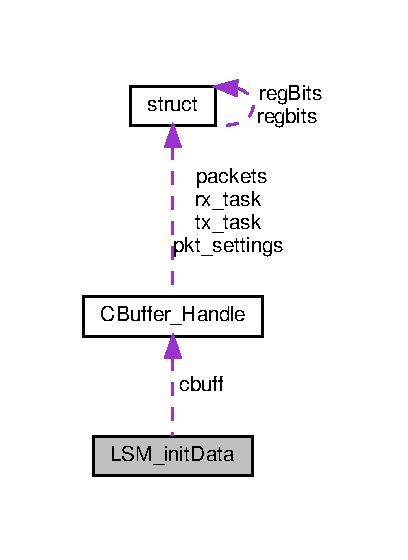
\includegraphics[width=196pt]{structLSM__initData__coll__graph}
\end{center}
\end{figure}
\subsection*{Public Attributes}
\begin{DoxyCompactItemize}
\item 
\mbox{\Hypertarget{structLSM__initData_a93ccee9247696ea65763e54a95352894}\label{structLSM__initData_a93ccee9247696ea65763e54a95352894}} 
gpio\+\_\+num\+\_\+t {\bfseries int1\+Pin}
\item 
gpio\+\_\+num\+\_\+t \hyperlink{structLSM__initData_a835c4e1a7a48cd95ef86123477e172d3}{int2\+Pin}
\item 
\hyperlink{vl53l0x__types_8h_aba7bc1797add20fe3efdf37ced1182c5}{uint8\+\_\+t} \hyperlink{structLSM__initData_a9742f792882a0ed6f85898600cf923b2}{comms\+Channel}
\item 
\hyperlink{vl53l0x__types_8h_aba7bc1797add20fe3efdf37ced1182c5}{uint8\+\_\+t} \hyperlink{structLSM__initData_a53b58c95bfcef402318923290252796a}{addr\+Pin\+State}
\item 
\mbox{\Hypertarget{structLSM__initData_ae12da731369c6ae103cf2c5cdd002989}\label{structLSM__initData_ae12da731369c6ae103cf2c5cdd002989}} 
L\+S\+M\+\_\+\+Device\+Comm\+Mode\+\_\+t {\bfseries comm\+Mode}
\item 
\mbox{\Hypertarget{structLSM__initData_a6e8a8c3e3ad8b92763e16e32942e86fc}\label{structLSM__initData_a6e8a8c3e3ad8b92763e16e32942e86fc}} 
L\+S\+M\+\_\+\+Operating\+Mode\+\_\+t {\bfseries op\+Mode}
\item 
\mbox{\Hypertarget{structLSM__initData_a303233d88db4314a2d773dae4106f8ea}\label{structLSM__initData_a303233d88db4314a2d773dae4106f8ea}} 
L\+S\+M\+\_\+\+Accel\+O\+D\+R\+\_\+t {\bfseries accel\+Rate}
\item 
\mbox{\Hypertarget{structLSM__initData_a5b35f43fcd684e7d12ac8513ae92c07e}\label{structLSM__initData_a5b35f43fcd684e7d12ac8513ae92c07e}} 
L\+S\+M\+\_\+\+Gyro\+O\+D\+R\+\_\+t {\bfseries gyro\+Rate}
\item 
\mbox{\Hypertarget{structLSM__initData_a81089885e0e3137a8e47cfd2d73c1884}\label{structLSM__initData_a81089885e0e3137a8e47cfd2d73c1884}} 
bool {\bfseries assign\+Fifo\+Buffer}
\item 
bool \hyperlink{structLSM__initData_a6daa9b9c11602e8b64c4a1f33ab03a2b}{use\+\_\+cbuffer}
\item 
\mbox{\Hypertarget{structLSM__initData_a86b0f56623fc9536c4776f604aebde6f}\label{structLSM__initData_a86b0f56623fc9536c4776f604aebde6f}} 
bool {\bfseries cbuff\+\_\+store\+\_\+raw}
\item 
\mbox{\Hypertarget{structLSM__initData_a537f3cd3b8f24fa83f82ed0b2bbb325d}\label{structLSM__initData_a537f3cd3b8f24fa83f82ed0b2bbb325d}} 
bool {\bfseries cbuff\+\_\+store\+\_\+packets}
\item 
\mbox{\Hypertarget{structLSM__initData_a5c5aa016c9f1ba95a2a336d96b97b4fd}\label{structLSM__initData_a5c5aa016c9f1ba95a2a336d96b97b4fd}} 
\hyperlink{structCBuffer__Handle}{C\+Buff} {\bfseries cbuff}
\end{DoxyCompactItemize}


\subsection{Detailed Description}
init\+Data struct
\begin{DoxyItemize}
\item keep it simple, let user configure with extra functions 
\end{DoxyItemize}

\subsection{Member Data Documentation}
\mbox{\Hypertarget{structLSM__initData_a53b58c95bfcef402318923290252796a}\label{structLSM__initData_a53b58c95bfcef402318923290252796a}} 
\index{L\+S\+M\+\_\+init\+Data@{L\+S\+M\+\_\+init\+Data}!addr\+Pin\+State@{addr\+Pin\+State}}
\index{addr\+Pin\+State@{addr\+Pin\+State}!L\+S\+M\+\_\+init\+Data@{L\+S\+M\+\_\+init\+Data}}
\subsubsection{\texorpdfstring{addr\+Pin\+State}{addrPinState}}
{\footnotesize\ttfamily \hyperlink{vl53l0x__types_8h_aba7bc1797add20fe3efdf37ced1182c5}{uint8\+\_\+t} L\+S\+M\+\_\+init\+Data\+::addr\+Pin\+State}

$<$ comms channel for i2c or spi \mbox{\Hypertarget{structLSM__initData_a9742f792882a0ed6f85898600cf923b2}\label{structLSM__initData_a9742f792882a0ed6f85898600cf923b2}} 
\index{L\+S\+M\+\_\+init\+Data@{L\+S\+M\+\_\+init\+Data}!comms\+Channel@{comms\+Channel}}
\index{comms\+Channel@{comms\+Channel}!L\+S\+M\+\_\+init\+Data@{L\+S\+M\+\_\+init\+Data}}
\subsubsection{\texorpdfstring{comms\+Channel}{commsChannel}}
{\footnotesize\ttfamily \hyperlink{vl53l0x__types_8h_aba7bc1797add20fe3efdf37ced1182c5}{uint8\+\_\+t} L\+S\+M\+\_\+init\+Data\+::comms\+Channel}

$<$ gpio pin for int 2 -\/ 0 if unused \mbox{\Hypertarget{structLSM__initData_a835c4e1a7a48cd95ef86123477e172d3}\label{structLSM__initData_a835c4e1a7a48cd95ef86123477e172d3}} 
\index{L\+S\+M\+\_\+init\+Data@{L\+S\+M\+\_\+init\+Data}!int2\+Pin@{int2\+Pin}}
\index{int2\+Pin@{int2\+Pin}!L\+S\+M\+\_\+init\+Data@{L\+S\+M\+\_\+init\+Data}}
\subsubsection{\texorpdfstring{int2\+Pin}{int2Pin}}
{\footnotesize\ttfamily gpio\+\_\+num\+\_\+t L\+S\+M\+\_\+init\+Data\+::int2\+Pin}

$<$ gpio pin for int 1 -\/ 0 if unused \mbox{\Hypertarget{structLSM__initData_a6daa9b9c11602e8b64c4a1f33ab03a2b}\label{structLSM__initData_a6daa9b9c11602e8b64c4a1f33ab03a2b}} 
\index{L\+S\+M\+\_\+init\+Data@{L\+S\+M\+\_\+init\+Data}!use\+\_\+cbuffer@{use\+\_\+cbuffer}}
\index{use\+\_\+cbuffer@{use\+\_\+cbuffer}!L\+S\+M\+\_\+init\+Data@{L\+S\+M\+\_\+init\+Data}}
\subsubsection{\texorpdfstring{use\+\_\+cbuffer}{use\_cbuffer}}
{\footnotesize\ttfamily bool L\+S\+M\+\_\+init\+Data\+::use\+\_\+cbuffer}

$<$ assign an 8\+Kb dma-\/cap buffer for burst fifo reads use cbuffer for fifo transactions -\/ usurps assign\+Fifo\+Buffer 

The documentation for this struct was generated from the following file\+:\begin{DoxyCompactItemize}
\item 
L\+S\+M\+\_\+\+Driver/L\+S\+M\+\_\+\+Driver.\+h\end{DoxyCompactItemize}

\hypertarget{structLSM__status}{}\section{L\+S\+M\+\_\+status Struct Reference}
\label{structLSM__status}\index{L\+S\+M\+\_\+status@{L\+S\+M\+\_\+status}}
\subsection*{Public Attributes}
\begin{DoxyCompactItemize}
\item 
\mbox{\Hypertarget{structLSM__status_ad625d0b1e5a64038e235047b52a5cb04}\label{structLSM__status_ad625d0b1e5a64038e235047b52a5cb04}} 
bool {\bfseries device\+\_\+rdy}
\item 
\mbox{\Hypertarget{structLSM__status_a87163366812a238903332a99ce0cb27f}\label{structLSM__status_a87163366812a238903332a99ce0cb27f}} 
bool {\bfseries accel\+\_\+drdy}
\item 
\mbox{\Hypertarget{structLSM__status_a7178acde664eb3e8c8f88878277dcf2f}\label{structLSM__status_a7178acde664eb3e8c8f88878277dcf2f}} 
bool {\bfseries gyro\+\_\+drdy}
\item 
\mbox{\Hypertarget{structLSM__status_a19bff2b3e7ab5e6234c373325ee84bad}\label{structLSM__status_a19bff2b3e7ab5e6234c373325ee84bad}} 
bool {\bfseries temp\+\_\+drdy}
\item 
\mbox{\Hypertarget{structLSM__status_adc8916440d8ce5de552d571ca53f2748}\label{structLSM__status_adc8916440d8ce5de552d571ca53f2748}} 
bool {\bfseries fifo\+\_\+rdy}
\item 
\mbox{\Hypertarget{structLSM__status_a1baec138f3c771116fa1bd5366c1148d}\label{structLSM__status_a1baec138f3c771116fa1bd5366c1148d}} 
bool {\bfseries step\+\_\+drdy}
\item 
\mbox{\Hypertarget{structLSM__status_a1b478b805466228e8134b1b9753cdfe4}\label{structLSM__status_a1b478b805466228e8134b1b9753cdfe4}} 
bool {\bfseries fifo\+\_\+full}
\item 
\mbox{\Hypertarget{structLSM__status_a1038a7382ad777148076467030f5c5d2}\label{structLSM__status_a1038a7382ad777148076467030f5c5d2}} 
bool {\bfseries fifo\+\_\+empty}
\item 
\mbox{\Hypertarget{structLSM__status_ae60fcf3017c4811d437e5f95ad435b57}\label{structLSM__status_ae60fcf3017c4811d437e5f95ad435b57}} 
bool {\bfseries fifo\+\_\+ovr}
\item 
\mbox{\Hypertarget{structLSM__status_a44701e6d51fa9ec895f928431e0ae9dc}\label{structLSM__status_a44701e6d51fa9ec895f928431e0ae9dc}} 
bool {\bfseries fifo\+\_\+thresh}
\end{DoxyCompactItemize}


The documentation for this struct was generated from the following file\+:\begin{DoxyCompactItemize}
\item 
L\+S\+M\+\_\+\+Driver/L\+S\+M\+\_\+\+Driver.\+h\end{DoxyCompactItemize}

\hypertarget{structMax30102__Driver}{}\section{Max30102\+\_\+\+Driver Struct Reference}
\label{structMax30102__Driver}\index{Max30102\+\_\+\+Driver@{Max30102\+\_\+\+Driver}}


Collaboration diagram for Max30102\+\_\+\+Driver\+:\nopagebreak
\begin{figure}[H]
\begin{center}
\leavevmode
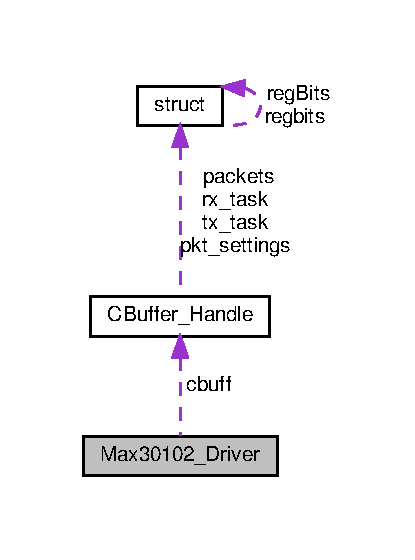
\includegraphics[width=199pt]{structMax30102__Driver__coll__graph}
\end{center}
\end{figure}
\subsection*{Public Attributes}
\begin{DoxyCompactItemize}
\item 
\mbox{\Hypertarget{structMax30102__Driver_ab7256133d2ce1d4380dc279e85179c6c}\label{structMax30102__Driver_ab7256133d2ce1d4380dc279e85179c6c}} 
\hyperlink{vl53l0x__types_8h_aba7bc1797add20fe3efdf37ced1182c5}{uint8\+\_\+t} {\bfseries dev\+\_\+addr}
\item 
\mbox{\Hypertarget{structMax30102__Driver_a7703972682ec7663797f36c5d23b4955}\label{structMax30102__Driver_a7703972682ec7663797f36c5d23b4955}} 
\hyperlink{vl53l0x__types_8h_aba7bc1797add20fe3efdf37ced1182c5}{uint8\+\_\+t} {\bfseries i2c\+\_\+bus}
\item 
\mbox{\Hypertarget{structMax30102__Driver_a9acd078dba5900d47c1c441d9d9c5127}\label{structMax30102__Driver_a9acd078dba5900d47c1c441d9d9c5127}} 
bool {\bfseries use\+\_\+cbuff}
\item 
\mbox{\Hypertarget{structMax30102__Driver_a613f044cbb4a18783bfe7baaf27c16d5}\label{structMax30102__Driver_a613f044cbb4a18783bfe7baaf27c16d5}} 
bool {\bfseries ambi\+\_\+ovr\+\_\+invalidates}
\item 
\mbox{\Hypertarget{structMax30102__Driver_ace2570e7a7086ca5ddbfb25f933e39b5}\label{structMax30102__Driver_ace2570e7a7086ca5ddbfb25f933e39b5}} 
bool {\bfseries drop\+\_\+next\+\_\+fifo}
\item 
\mbox{\Hypertarget{structMax30102__Driver_aae09389193cfc8f08f89eccf1196a8e8}\label{structMax30102__Driver_aae09389193cfc8f08f89eccf1196a8e8}} 
gpio\+\_\+num\+\_\+t {\bfseries intr\+\_\+pin}
\item 
\mbox{\Hypertarget{structMax30102__Driver_a4f839052dc0bcf51c7cf0796a62b2ebf}\label{structMax30102__Driver_a4f839052dc0bcf51c7cf0796a62b2ebf}} 
Task\+Handle\+\_\+t {\bfseries taskhandle}
\item 
\mbox{\Hypertarget{structMax30102__Driver_a711c9ed4c0c6c8d538afa2d43b834591}\label{structMax30102__Driver_a711c9ed4c0c6c8d538afa2d43b834591}} 
\hyperlink{vl53l0x__types_8h_aba7bc1797add20fe3efdf37ced1182c5}{uint8\+\_\+t} {\bfseries intr\+\_\+mask}
\item 
\mbox{\Hypertarget{structMax30102__Driver_a2bdfe690b862f30a92d0c92347687548}\label{structMax30102__Driver_a2bdfe690b862f30a92d0c92347687548}} 
\hyperlink{vl53l0x__types_8h_aba7bc1797add20fe3efdf37ced1182c5}{uint8\+\_\+t} {\bfseries led\+I\+R\+\_\+ampl}
\item 
\mbox{\Hypertarget{structMax30102__Driver_ab74522dea5e1102404300aae4963d3af}\label{structMax30102__Driver_ab74522dea5e1102404300aae4963d3af}} 
\hyperlink{vl53l0x__types_8h_aba7bc1797add20fe3efdf37ced1182c5}{uint8\+\_\+t} {\bfseries led\+Red\+\_\+ampl}
\item 
\mbox{\Hypertarget{structMax30102__Driver_ad6bd7a4c94296d2549c4278de7bf01a2}\label{structMax30102__Driver_ad6bd7a4c94296d2549c4278de7bf01a2}} 
bool {\bfseries shutdown}
\item 
\mbox{\Hypertarget{structMax30102__Driver_af0dcd585b3697a2b20f258ba7d861e93}\label{structMax30102__Driver_af0dcd585b3697a2b20f258ba7d861e93}} 
bool {\bfseries use\+\_\+fifo}
\item 
\mbox{\Hypertarget{structMax30102__Driver_abafb755b7e3ec393b30ea732dbe34a80}\label{structMax30102__Driver_abafb755b7e3ec393b30ea732dbe34a80}} 
bool {\bfseries fifo\+\_\+ovr}
\item 
\mbox{\Hypertarget{structMax30102__Driver_a4a06fa87fe1693456b43e978510cc694}\label{structMax30102__Driver_a4a06fa87fe1693456b43e978510cc694}} 
max31\+\_\+mode\+\_\+t {\bfseries device\+\_\+mode}
\item 
\mbox{\Hypertarget{structMax30102__Driver_a36535395c51d3d5e5e80d17d252d88a6}\label{structMax30102__Driver_a36535395c51d3d5e5e80d17d252d88a6}} 
max31\+\_\+sampleavg\+\_\+t {\bfseries smpavg}
\item 
\mbox{\Hypertarget{structMax30102__Driver_a47573b2c998f49ee520ab88d6ac52f4e}\label{structMax30102__Driver_a47573b2c998f49ee520ab88d6ac52f4e}} 
\hyperlink{vl53l0x__types_8h_aba7bc1797add20fe3efdf37ced1182c5}{uint8\+\_\+t} {\bfseries almostfull}
\item 
\mbox{\Hypertarget{structMax30102__Driver_ac4d5954ee975cb5e122f8ea1ce0380e8}\label{structMax30102__Driver_ac4d5954ee975cb5e122f8ea1ce0380e8}} 
max31\+\_\+samplerate\+\_\+t {\bfseries samplerate}
\item 
\mbox{\Hypertarget{structMax30102__Driver_ac808d5dfe66cd1ca93e2989fc81748c1}\label{structMax30102__Driver_ac808d5dfe66cd1ca93e2989fc81748c1}} 
max31\+\_\+ledpwm\+\_\+t {\bfseries ledpwm}
\item 
\mbox{\Hypertarget{structMax30102__Driver_a22622d5d9a6c088e5339d0f1d086c7fd}\label{structMax30102__Driver_a22622d5d9a6c088e5339d0f1d086c7fd}} 
max31\+\_\+adcrange\+\_\+t {\bfseries adcrange}
\item 
\mbox{\Hypertarget{structMax30102__Driver_af75824f0fbce881d69f70fdeb13e8755}\label{structMax30102__Driver_af75824f0fbce881d69f70fdeb13e8755}} 
\hyperlink{vl53l0x__types_8h_aba7bc1797add20fe3efdf37ced1182c5}{uint8\+\_\+t} {\bfseries red\+\_\+lvl}
\item 
\mbox{\Hypertarget{structMax30102__Driver_af67fe57f1459e33c5ea3ee20143bf21a}\label{structMax30102__Driver_af67fe57f1459e33c5ea3ee20143bf21a}} 
bool {\bfseries temp\+\_\+sampling}
\item 
\mbox{\Hypertarget{structMax30102__Driver_aa2932ea4391a2345c27e5ac5b14ccbd6}\label{structMax30102__Driver_aa2932ea4391a2345c27e5ac5b14ccbd6}} 
\hyperlink{vl53l0x__types_8h_aba7bc1797add20fe3efdf37ced1182c5}{uint8\+\_\+t} {\bfseries fifo\+\_\+buffer} \mbox{[}M\+A\+X31\+\_\+\+F\+I\+F\+O\+\_\+\+M\+A\+X\+\_\+\+S\+I\+ZE\mbox{]}
\item 
\mbox{\Hypertarget{structMax30102__Driver_a504a6683ab569174046fe1c581aea4b9}\label{structMax30102__Driver_a504a6683ab569174046fe1c581aea4b9}} 
\hyperlink{vl53l0x__types_8h_aba7bc1797add20fe3efdf37ced1182c5}{uint8\+\_\+t} {\bfseries bytes\+\_\+read}
\item 
\mbox{\Hypertarget{structMax30102__Driver_ad52aa33c8ad19cacde285e3f30ec690e}\label{structMax30102__Driver_ad52aa33c8ad19cacde285e3f30ec690e}} 
float {\bfseries red\+\_\+buffer} \mbox{[}M\+A\+X31\+\_\+\+F\+I\+F\+O\+\_\+\+S\+A\+M\+P\+L\+ES\mbox{]}
\item 
\mbox{\Hypertarget{structMax30102__Driver_ad3e81de48c6c2e2546f87a63088db43e}\label{structMax30102__Driver_ad3e81de48c6c2e2546f87a63088db43e}} 
float {\bfseries ir\+\_\+buffer} \mbox{[}M\+A\+X31\+\_\+\+F\+I\+F\+O\+\_\+\+S\+A\+M\+P\+L\+ES\mbox{]}
\item 
\mbox{\Hypertarget{structMax30102__Driver_ac665c199687f1a405e4c73ff582a3782}\label{structMax30102__Driver_ac665c199687f1a405e4c73ff582a3782}} 
\hyperlink{vl53l0x__types_8h_aba7bc1797add20fe3efdf37ced1182c5}{uint8\+\_\+t} {\bfseries pkts\+\_\+in\+\_\+fifo}
\item 
\mbox{\Hypertarget{structMax30102__Driver_aac42ca7ba8f056d2728e052fa0e662c8}\label{structMax30102__Driver_aac42ca7ba8f056d2728e052fa0e662c8}} 
max31\+\_\+drivermode\+\_\+t {\bfseries drivermode}
\item 
\mbox{\Hypertarget{structMax30102__Driver_a23c693c9e6fd29315f54f54b44e51d51}\label{structMax30102__Driver_a23c693c9e6fd29315f54f54b44e51d51}} 
bool {\bfseries configured}
\item 
\mbox{\Hypertarget{structMax30102__Driver_adfdc2f3abf96d7620a3a0e96d4475678}\label{structMax30102__Driver_adfdc2f3abf96d7620a3a0e96d4475678}} 
float {\bfseries temperature}
\item 
\mbox{\Hypertarget{structMax30102__Driver_adee3ef5c399951219c44191cee97ebb7}\label{structMax30102__Driver_adee3ef5c399951219c44191cee97ebb7}} 
\hyperlink{vl53l0x__types_8h_a435d1572bf3f880d55459d9805097f62}{uint32\+\_\+t} {\bfseries ticks\+\_\+since\+\_\+temperature}
\item 
\mbox{\Hypertarget{structMax30102__Driver_aed83761f4f5e3c83cea69b60ea139b67}\label{structMax30102__Driver_aed83761f4f5e3c83cea69b60ea139b67}} 
\hyperlink{structCBuffer__Handle}{C\+Buff} {\bfseries cbuff}
\end{DoxyCompactItemize}


The documentation for this struct was generated from the following file\+:\begin{DoxyCompactItemize}
\item 
Max30102\+\_\+\+Driver/Max30102\+\_\+\+Driver.\+h\end{DoxyCompactItemize}

\hypertarget{structmax31__initdata}{}\section{max31\+\_\+initdata Struct Reference}
\label{structmax31__initdata}\index{max31\+\_\+initdata@{max31\+\_\+initdata}}


Collaboration diagram for max31\+\_\+initdata\+:\nopagebreak
\begin{figure}[H]
\begin{center}
\leavevmode
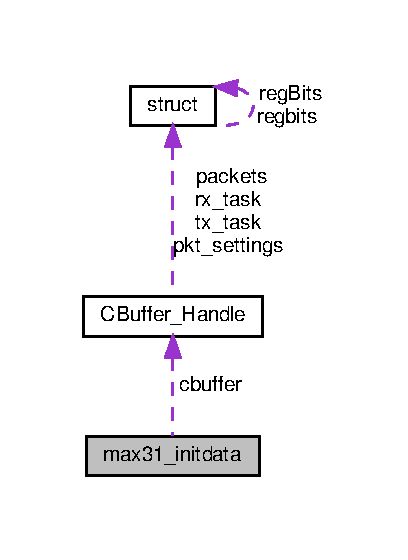
\includegraphics[width=196pt]{structmax31__initdata__coll__graph}
\end{center}
\end{figure}
\subsection*{Public Attributes}
\begin{DoxyCompactItemize}
\item 
\mbox{\Hypertarget{structmax31__initdata_ab5db3540298afbf9a8c8daf16d8c8ae9}\label{structmax31__initdata_ab5db3540298afbf9a8c8daf16d8c8ae9}} 
\hyperlink{vl53l0x__types_8h_aba7bc1797add20fe3efdf37ced1182c5}{uint8\+\_\+t} {\bfseries i2c\+\_\+bus}
\item 
\mbox{\Hypertarget{structmax31__initdata_a860bfc03e8c60fb5874cbbb7738e4e06}\label{structmax31__initdata_a860bfc03e8c60fb5874cbbb7738e4e06}} 
gpio\+\_\+num\+\_\+t {\bfseries intr\+\_\+pin}
\item 
\mbox{\Hypertarget{structmax31__initdata_a76583a0592895644e43f89a93e47cde1}\label{structmax31__initdata_a76583a0592895644e43f89a93e47cde1}} 
bool {\bfseries use\+\_\+cbuffer}
\item 
\mbox{\Hypertarget{structmax31__initdata_a4ddb43c043327642a95058ce4d6eb235}\label{structmax31__initdata_a4ddb43c043327642a95058ce4d6eb235}} 
\hyperlink{structCBuffer__Handle}{C\+Buff} {\bfseries cbuffer}
\end{DoxyCompactItemize}


The documentation for this struct was generated from the following file\+:\begin{DoxyCompactItemize}
\item 
Max30102\+\_\+\+Driver/Max30102\+\_\+\+Driver.\+h\end{DoxyCompactItemize}

\hypertarget{structMFRC__Init}{}\section{M\+F\+R\+C\+\_\+\+Init Struct Reference}
\label{structMFRC__Init}\index{M\+F\+R\+C\+\_\+\+Init@{M\+F\+R\+C\+\_\+\+Init}}
\subsection*{Public Attributes}
\begin{DoxyCompactItemize}
\item 
\mbox{\Hypertarget{structMFRC__Init_a5f0bbc528912b4a8d95b964dcde31837}\label{structMFRC__Init_a5f0bbc528912b4a8d95b964dcde31837}} 
\hyperlink{vl53l0x__types_8h_aba7bc1797add20fe3efdf37ced1182c5}{uint8\+\_\+t} {\bfseries comms\+\_\+bus}
\item 
\mbox{\Hypertarget{structMFRC__Init_a98dfa94adfc08ed5bd7c28d90ec34862}\label{structMFRC__Init_a98dfa94adfc08ed5bd7c28d90ec34862}} 
mfrc\+\_\+comms\+\_\+mode\+\_\+t {\bfseries comms\+\_\+mode}
\item 
\mbox{\Hypertarget{structMFRC__Init_a6e9c5405f2685795509f68a9263f3a12}\label{structMFRC__Init_a6e9c5405f2685795509f68a9263f3a12}} 
gpio\+\_\+num\+\_\+t {\bfseries rst\+\_\+pin}
\item 
\mbox{\Hypertarget{structMFRC__Init_a3a2a8c560083711e218a8e1e5d4aac99}\label{structMFRC__Init_a3a2a8c560083711e218a8e1e5d4aac99}} 
gpio\+\_\+num\+\_\+t {\bfseries irq\+\_\+pin}
\end{DoxyCompactItemize}


The documentation for this struct was generated from the following file\+:\begin{DoxyCompactItemize}
\item 
M\+F\+R\+C522\+\_\+\+Driver/M\+F\+R\+C522\+\_\+\+Driver.\+h\end{DoxyCompactItemize}

\hypertarget{structmsg__handle}{}\section{msg\+\_\+handle Struct Reference}
\label{structmsg__handle}\index{msg\+\_\+handle@{msg\+\_\+handle}}


Collaboration diagram for msg\+\_\+handle\+:\nopagebreak
\begin{figure}[H]
\begin{center}
\leavevmode
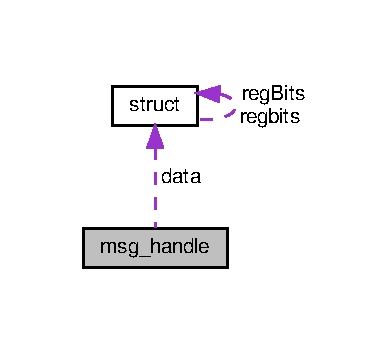
\includegraphics[width=187pt]{structmsg__handle__coll__graph}
\end{center}
\end{figure}
\subsection*{Public Attributes}
\begin{DoxyCompactItemize}
\item 
gpio\+\_\+num\+\_\+t \hyperlink{structmsg__handle_a6ecce9c5946c5ea3abf2f6a03a3a56d4}{data\+\_\+pin}
\item 
gpio\+\_\+num\+\_\+t \hyperlink{structmsg__handle_ad94640677937313338f02b7f5028d1eb}{rst\+\_\+pin}
\item 
gpio\+\_\+num\+\_\+t \hyperlink{structmsg__handle_a63d6c0448a1ade1b6713b385b1d48fa5}{strobe\+\_\+pin}
\item 
adc\+\_\+channel\+\_\+t \hyperlink{structmsg__handle_abe01e1ee941e2bec055bc2dc49b012d7}{adc\+\_\+channel}
\item 
adc\+\_\+bits\+\_\+width\+\_\+t \hyperlink{structmsg__handle_acab455fa1ecba62ef057c6ff402f4e56}{adc\+\_\+bits}
\item 
bool \hyperlink{structmsg__handle_aef7fc68f0d9d9029114e84c241581d3e}{autosample}
\item 
\hyperlink{vl53l0x__types_8h_a273cf69d639a59973b6019625df33e30}{uint16\+\_\+t} \hyperlink{structmsg__handle_aa33b97382eac6687734713ec1748f01d}{autosample\+\_\+period\+\_\+ms}
\item 
Task\+Handle\+\_\+t \hyperlink{structmsg__handle_a7da2ef315ab07363c565ef5f745f6888}{task}
\item 
Timer\+Handle\+\_\+t \hyperlink{structmsg__handle_a1a3b5ad7116584ac06779562d8b41ec2}{timer}
\item 
\hyperlink{vl53l0x__types_8h_a273cf69d639a59973b6019625df33e30}{uint16\+\_\+t} \hyperlink{structmsg__handle_aa5ad7cd77c31f44c49a979bfda5a65ba}{pulse\+\_\+count}
\item 
\hyperlink{vl53l0x__types_8h_a273cf69d639a59973b6019625df33e30}{uint16\+\_\+t} \hyperlink{structmsg__handle_aa813acda542b8df85aff47b8c481b636}{reset\+\_\+n}
\item 
\mbox{\Hypertarget{structmsg__handle_a73fe56492bd18326849ce81f59d50f27}\label{structmsg__handle_a73fe56492bd18326849ce81f59d50f27}} 
bool {\bfseries enable\+\_\+oversample}
\item 
\mbox{\Hypertarget{structmsg__handle_a3673348c0666fb2d7b8c67a2744a6b88}\label{structmsg__handle_a3673348c0666fb2d7b8c67a2744a6b88}} 
\hyperlink{vl53l0x__types_8h_aba7bc1797add20fe3efdf37ced1182c5}{uint8\+\_\+t} {\bfseries oversample\+\_\+factor}
\item 
\hyperlink{structMSGEQ7__Measures}{msg\+\_\+measure\+\_\+t} \hyperlink{structmsg__handle_ab8254aa210bf3218eb7c5aeae4751a76}{data}
\end{DoxyCompactItemize}


\subsection{Member Data Documentation}
\mbox{\Hypertarget{structmsg__handle_acab455fa1ecba62ef057c6ff402f4e56}\label{structmsg__handle_acab455fa1ecba62ef057c6ff402f4e56}} 
\index{msg\+\_\+handle@{msg\+\_\+handle}!adc\+\_\+bits@{adc\+\_\+bits}}
\index{adc\+\_\+bits@{adc\+\_\+bits}!msg\+\_\+handle@{msg\+\_\+handle}}
\subsubsection{\texorpdfstring{adc\+\_\+bits}{adc\_bits}}
{\footnotesize\ttfamily adc\+\_\+bits\+\_\+width\+\_\+t msg\+\_\+handle\+::adc\+\_\+bits}

adc resolution \mbox{\Hypertarget{structmsg__handle_abe01e1ee941e2bec055bc2dc49b012d7}\label{structmsg__handle_abe01e1ee941e2bec055bc2dc49b012d7}} 
\index{msg\+\_\+handle@{msg\+\_\+handle}!adc\+\_\+channel@{adc\+\_\+channel}}
\index{adc\+\_\+channel@{adc\+\_\+channel}!msg\+\_\+handle@{msg\+\_\+handle}}
\subsubsection{\texorpdfstring{adc\+\_\+channel}{adc\_channel}}
{\footnotesize\ttfamily adc\+\_\+channel\+\_\+t msg\+\_\+handle\+::adc\+\_\+channel}

adc channel used on pin \mbox{\Hypertarget{structmsg__handle_aef7fc68f0d9d9029114e84c241581d3e}\label{structmsg__handle_aef7fc68f0d9d9029114e84c241581d3e}} 
\index{msg\+\_\+handle@{msg\+\_\+handle}!autosample@{autosample}}
\index{autosample@{autosample}!msg\+\_\+handle@{msg\+\_\+handle}}
\subsubsection{\texorpdfstring{autosample}{autosample}}
{\footnotesize\ttfamily bool msg\+\_\+handle\+::autosample}

automatically sample at rate specified \mbox{\Hypertarget{structmsg__handle_aa33b97382eac6687734713ec1748f01d}\label{structmsg__handle_aa33b97382eac6687734713ec1748f01d}} 
\index{msg\+\_\+handle@{msg\+\_\+handle}!autosample\+\_\+period\+\_\+ms@{autosample\+\_\+period\+\_\+ms}}
\index{autosample\+\_\+period\+\_\+ms@{autosample\+\_\+period\+\_\+ms}!msg\+\_\+handle@{msg\+\_\+handle}}
\subsubsection{\texorpdfstring{autosample\+\_\+period\+\_\+ms}{autosample\_period\_ms}}
{\footnotesize\ttfamily \hyperlink{vl53l0x__types_8h_a273cf69d639a59973b6019625df33e30}{uint16\+\_\+t} msg\+\_\+handle\+::autosample\+\_\+period\+\_\+ms}

period between each sample \mbox{\Hypertarget{structmsg__handle_ab8254aa210bf3218eb7c5aeae4751a76}\label{structmsg__handle_ab8254aa210bf3218eb7c5aeae4751a76}} 
\index{msg\+\_\+handle@{msg\+\_\+handle}!data@{data}}
\index{data@{data}!msg\+\_\+handle@{msg\+\_\+handle}}
\subsubsection{\texorpdfstring{data}{data}}
{\footnotesize\ttfamily \hyperlink{structMSGEQ7__Measures}{msg\+\_\+measure\+\_\+t} msg\+\_\+handle\+::data}

latest sampled data from device \mbox{\Hypertarget{structmsg__handle_a6ecce9c5946c5ea3abf2f6a03a3a56d4}\label{structmsg__handle_a6ecce9c5946c5ea3abf2f6a03a3a56d4}} 
\index{msg\+\_\+handle@{msg\+\_\+handle}!data\+\_\+pin@{data\+\_\+pin}}
\index{data\+\_\+pin@{data\+\_\+pin}!msg\+\_\+handle@{msg\+\_\+handle}}
\subsubsection{\texorpdfstring{data\+\_\+pin}{data\_pin}}
{\footnotesize\ttfamily gpio\+\_\+num\+\_\+t msg\+\_\+handle\+::data\+\_\+pin}

pin connected to data output of chip \mbox{\Hypertarget{structmsg__handle_aa5ad7cd77c31f44c49a979bfda5a65ba}\label{structmsg__handle_aa5ad7cd77c31f44c49a979bfda5a65ba}} 
\index{msg\+\_\+handle@{msg\+\_\+handle}!pulse\+\_\+count@{pulse\+\_\+count}}
\index{pulse\+\_\+count@{pulse\+\_\+count}!msg\+\_\+handle@{msg\+\_\+handle}}
\subsubsection{\texorpdfstring{pulse\+\_\+count}{pulse\_count}}
{\footnotesize\ttfamily \hyperlink{vl53l0x__types_8h_a273cf69d639a59973b6019625df33e30}{uint16\+\_\+t} msg\+\_\+handle\+::pulse\+\_\+count}

pulses since last reset \mbox{\Hypertarget{structmsg__handle_aa813acda542b8df85aff47b8c481b636}\label{structmsg__handle_aa813acda542b8df85aff47b8c481b636}} 
\index{msg\+\_\+handle@{msg\+\_\+handle}!reset\+\_\+n@{reset\+\_\+n}}
\index{reset\+\_\+n@{reset\+\_\+n}!msg\+\_\+handle@{msg\+\_\+handle}}
\subsubsection{\texorpdfstring{reset\+\_\+n}{reset\_n}}
{\footnotesize\ttfamily \hyperlink{vl53l0x__types_8h_a273cf69d639a59973b6019625df33e30}{uint16\+\_\+t} msg\+\_\+handle\+::reset\+\_\+n}

number of reads between resets \mbox{\Hypertarget{structmsg__handle_ad94640677937313338f02b7f5028d1eb}\label{structmsg__handle_ad94640677937313338f02b7f5028d1eb}} 
\index{msg\+\_\+handle@{msg\+\_\+handle}!rst\+\_\+pin@{rst\+\_\+pin}}
\index{rst\+\_\+pin@{rst\+\_\+pin}!msg\+\_\+handle@{msg\+\_\+handle}}
\subsubsection{\texorpdfstring{rst\+\_\+pin}{rst\_pin}}
{\footnotesize\ttfamily gpio\+\_\+num\+\_\+t msg\+\_\+handle\+::rst\+\_\+pin}

pin connected to the reset pin of chip \mbox{\Hypertarget{structmsg__handle_a63d6c0448a1ade1b6713b385b1d48fa5}\label{structmsg__handle_a63d6c0448a1ade1b6713b385b1d48fa5}} 
\index{msg\+\_\+handle@{msg\+\_\+handle}!strobe\+\_\+pin@{strobe\+\_\+pin}}
\index{strobe\+\_\+pin@{strobe\+\_\+pin}!msg\+\_\+handle@{msg\+\_\+handle}}
\subsubsection{\texorpdfstring{strobe\+\_\+pin}{strobe\_pin}}
{\footnotesize\ttfamily gpio\+\_\+num\+\_\+t msg\+\_\+handle\+::strobe\+\_\+pin}

pin connected to the strobe pin of chip \mbox{\Hypertarget{structmsg__handle_a7da2ef315ab07363c565ef5f745f6888}\label{structmsg__handle_a7da2ef315ab07363c565ef5f745f6888}} 
\index{msg\+\_\+handle@{msg\+\_\+handle}!task@{task}}
\index{task@{task}!msg\+\_\+handle@{msg\+\_\+handle}}
\subsubsection{\texorpdfstring{task}{task}}
{\footnotesize\ttfamily Task\+Handle\+\_\+t msg\+\_\+handle\+::task}

driver task handle \mbox{\Hypertarget{structmsg__handle_a1a3b5ad7116584ac06779562d8b41ec2}\label{structmsg__handle_a1a3b5ad7116584ac06779562d8b41ec2}} 
\index{msg\+\_\+handle@{msg\+\_\+handle}!timer@{timer}}
\index{timer@{timer}!msg\+\_\+handle@{msg\+\_\+handle}}
\subsubsection{\texorpdfstring{timer}{timer}}
{\footnotesize\ttfamily Timer\+Handle\+\_\+t msg\+\_\+handle\+::timer}

driver timer handle 

The documentation for this struct was generated from the following file\+:\begin{DoxyCompactItemize}
\item 
M\+S\+G\+E\+Q7\+\_\+\+Driver/M\+S\+G\+E\+Q7\+\_\+\+Driver.\+h\end{DoxyCompactItemize}

\hypertarget{structmsg__init}{}\section{msg\+\_\+init Struct Reference}
\label{structmsg__init}\index{msg\+\_\+init@{msg\+\_\+init}}
\subsection*{Public Attributes}
\begin{DoxyCompactItemize}
\item 
\mbox{\Hypertarget{structmsg__init_a8269e8997a7a9049f08b8c30b64527bf}\label{structmsg__init_a8269e8997a7a9049f08b8c30b64527bf}} 
gpio\+\_\+num\+\_\+t {\bfseries data}
\item 
\mbox{\Hypertarget{structmsg__init_a74b3ce974e8bdeccc0c3e6ab0f20496b}\label{structmsg__init_a74b3ce974e8bdeccc0c3e6ab0f20496b}} 
gpio\+\_\+num\+\_\+t {\bfseries rst}
\item 
\mbox{\Hypertarget{structmsg__init_ab5fb9c86ad07f955541eaa8fb4edd852}\label{structmsg__init_ab5fb9c86ad07f955541eaa8fb4edd852}} 
gpio\+\_\+num\+\_\+t {\bfseries strobe}
\item 
\mbox{\Hypertarget{structmsg__init_a75c28e82034b4181d88d9e22d4df798e}\label{structmsg__init_a75c28e82034b4181d88d9e22d4df798e}} 
adc\+\_\+bits\+\_\+width\+\_\+t {\bfseries adc\+\_\+width}
\end{DoxyCompactItemize}


The documentation for this struct was generated from the following file\+:\begin{DoxyCompactItemize}
\item 
M\+S\+G\+E\+Q7\+\_\+\+Driver/M\+S\+G\+E\+Q7\+\_\+\+Driver.\+h\end{DoxyCompactItemize}

\hypertarget{structMSGEQ7__Measures}{}\section{M\+S\+G\+E\+Q7\+\_\+\+Measures Struct Reference}
\label{structMSGEQ7__Measures}\index{M\+S\+G\+E\+Q7\+\_\+\+Measures@{M\+S\+G\+E\+Q7\+\_\+\+Measures}}
\subsection*{Public Attributes}
\begin{DoxyCompactItemize}
\item 
\mbox{\Hypertarget{structMSGEQ7__Measures_abf7a7389a3e93776cdcb12b21c7857ee}\label{structMSGEQ7__Measures_abf7a7389a3e93776cdcb12b21c7857ee}} 
\hyperlink{vl53l0x__types_8h_aa343fa3b3d06292b959ffdd4c4703b06}{int16\+\_\+t} {\bfseries band\+\_\+1}
\item 
\mbox{\Hypertarget{structMSGEQ7__Measures_adb0257b35822e14d3e178b8a479cfb41}\label{structMSGEQ7__Measures_adb0257b35822e14d3e178b8a479cfb41}} 
\hyperlink{vl53l0x__types_8h_aa343fa3b3d06292b959ffdd4c4703b06}{int16\+\_\+t} {\bfseries band\+\_\+2}
\item 
\mbox{\Hypertarget{structMSGEQ7__Measures_af1e724e82ceae527b9f5d28fdd5d4280}\label{structMSGEQ7__Measures_af1e724e82ceae527b9f5d28fdd5d4280}} 
\hyperlink{vl53l0x__types_8h_aa343fa3b3d06292b959ffdd4c4703b06}{int16\+\_\+t} {\bfseries band\+\_\+3}
\item 
\mbox{\Hypertarget{structMSGEQ7__Measures_a4a385d30f0900c30ac466feb5562f0cf}\label{structMSGEQ7__Measures_a4a385d30f0900c30ac466feb5562f0cf}} 
\hyperlink{vl53l0x__types_8h_aa343fa3b3d06292b959ffdd4c4703b06}{int16\+\_\+t} {\bfseries band\+\_\+4}
\item 
\mbox{\Hypertarget{structMSGEQ7__Measures_a442019a7bf80453d3d0f810f0070be70}\label{structMSGEQ7__Measures_a442019a7bf80453d3d0f810f0070be70}} 
\hyperlink{vl53l0x__types_8h_aa343fa3b3d06292b959ffdd4c4703b06}{int16\+\_\+t} {\bfseries band\+\_\+5}
\item 
\mbox{\Hypertarget{structMSGEQ7__Measures_a0343968e95e0ce21e3ce20a67fd1f9e5}\label{structMSGEQ7__Measures_a0343968e95e0ce21e3ce20a67fd1f9e5}} 
\hyperlink{vl53l0x__types_8h_aa343fa3b3d06292b959ffdd4c4703b06}{int16\+\_\+t} {\bfseries band\+\_\+6}
\item 
\mbox{\Hypertarget{structMSGEQ7__Measures_a0cdeb7acb6506501e0f4712f2736b621}\label{structMSGEQ7__Measures_a0cdeb7acb6506501e0f4712f2736b621}} 
\hyperlink{vl53l0x__types_8h_aa343fa3b3d06292b959ffdd4c4703b06}{int16\+\_\+t} {\bfseries band\+\_\+7}
\item 
\mbox{\Hypertarget{structMSGEQ7__Measures_acde0b37f97ff786cbf190b430f54e356}\label{structMSGEQ7__Measures_acde0b37f97ff786cbf190b430f54e356}} 
\hyperlink{vl53l0x__types_8h_a273cf69d639a59973b6019625df33e30}{uint16\+\_\+t} {\bfseries base\+\_\+levels} \mbox{[}7\mbox{]}
\end{DoxyCompactItemize}


The documentation for this struct was generated from the following file\+:\begin{DoxyCompactItemize}
\item 
M\+S\+G\+E\+Q7\+\_\+\+Driver/M\+S\+G\+E\+Q7\+\_\+\+Driver.\+h\end{DoxyCompactItemize}

\hypertarget{structprx__settings__t}{}\section{prx\+\_\+settings\+\_\+t Struct Reference}
\label{structprx__settings__t}\index{prx\+\_\+settings\+\_\+t@{prx\+\_\+settings\+\_\+t}}


\hyperlink{structThe}{The} driver\textquotesingle{}s Proximity settings.  




{\ttfamily \#include $<$A\+P\+D\+S9960\+\_\+\+Driver.\+h$>$}



\subsection{Detailed Description}
\hyperlink{structThe}{The} driver\textquotesingle{}s Proximity settings. 

The documentation for this struct was generated from the following file\+:\begin{DoxyCompactItemize}
\item 
A\+P\+D\+S9960\+\_\+\+Driver/A\+P\+D\+S9960\+\_\+\+Driver.\+h\end{DoxyCompactItemize}

\hypertarget{structRGB__Driver}{}\section{R\+G\+B\+\_\+\+Driver Struct Reference}
\label{structRGB__Driver}\index{R\+G\+B\+\_\+\+Driver@{R\+G\+B\+\_\+\+Driver}}
\subsection*{Public Attributes}
\begin{DoxyCompactItemize}
\item 
gpio\+\_\+num\+\_\+t \hyperlink{structRGB__Driver_a899a4207afcd1b6b3dc55e9dbcc4b9ee}{r\+\_\+channel}
\item 
gpio\+\_\+num\+\_\+t \hyperlink{structRGB__Driver_a9c39550796d8bcd79beefdc4faac485f}{g\+\_\+channel}
\item 
gpio\+\_\+num\+\_\+t \hyperlink{structRGB__Driver_a2ce6a8d15b7a1411f68cd26c67e8cd4a}{b\+\_\+channel}
\item 
bool \hyperlink{structRGB__Driver_a37da49d052a49bd9e57357bdab8c0591}{active\+\_\+level}
\item 
\mbox{\Hypertarget{structRGB__Driver_a8f868b5b0af48e661af85c30e6302a59}\label{structRGB__Driver_a8f868b5b0af48e661af85c30e6302a59}} 
\hyperlink{vl53l0x__types_8h_a435d1572bf3f880d55459d9805097f62}{uint32\+\_\+t} {\bfseries fade\+\_\+time}
\item 
\hyperlink{vl53l0x__types_8h_a435d1572bf3f880d55459d9805097f62}{uint32\+\_\+t} \hyperlink{structRGB__Driver_a2d794ede506e3bb49b2f3ae4c772c418}{resolution}
\item 
\hyperlink{vl53l0x__types_8h_a435d1572bf3f880d55459d9805097f62}{uint32\+\_\+t} \hyperlink{structRGB__Driver_a664e5a2dbe8b040241fa1296970df9a7}{frequency}
\item 
\mbox{\Hypertarget{structRGB__Driver_a09a465ffbc633a5dcf33a586d3f97cd0}\label{structRGB__Driver_a09a465ffbc633a5dcf33a586d3f97cd0}} 
\hyperlink{vl53l0x__types_8h_a435d1572bf3f880d55459d9805097f62}{uint32\+\_\+t} {\bfseries max\+\_\+duty}
\item 
\hyperlink{vl53l0x__types_8h_a435d1572bf3f880d55459d9805097f62}{uint32\+\_\+t} \hyperlink{structRGB__Driver_a66dea398a8883deef0901c71be75a980}{r\+\_\+duty}
\item 
\hyperlink{vl53l0x__types_8h_a435d1572bf3f880d55459d9805097f62}{uint32\+\_\+t} \hyperlink{structRGB__Driver_a0b3b1c3bfbc55af8155a6224a9d247a4}{g\+\_\+duty}
\item 
\hyperlink{vl53l0x__types_8h_a435d1572bf3f880d55459d9805097f62}{uint32\+\_\+t} \hyperlink{structRGB__Driver_ab0a18173b1c3080386c2a2439d04befd}{b\+\_\+duty}
\item 
\mbox{\Hypertarget{structRGB__Driver_aa07486be8ddf6e6b94681f8422bd7119}\label{structRGB__Driver_aa07486be8ddf6e6b94681f8422bd7119}} 
\hyperlink{vl53l0x__types_8h_aba7bc1797add20fe3efdf37ced1182c5}{uint8\+\_\+t} {\bfseries r\+\_\+val}
\item 
\mbox{\Hypertarget{structRGB__Driver_a5e566b01cae790c03581d65e53399339}\label{structRGB__Driver_a5e566b01cae790c03581d65e53399339}} 
\hyperlink{vl53l0x__types_8h_aba7bc1797add20fe3efdf37ced1182c5}{uint8\+\_\+t} {\bfseries g\+\_\+val}
\item 
\mbox{\Hypertarget{structRGB__Driver_a9d30d72e88f462b2ae983cc2e04e79e1}\label{structRGB__Driver_a9d30d72e88f462b2ae983cc2e04e79e1}} 
\hyperlink{vl53l0x__types_8h_aba7bc1797add20fe3efdf37ced1182c5}{uint8\+\_\+t} {\bfseries b\+\_\+val}
\item 
\mbox{\Hypertarget{structRGB__Driver_ac431da42eec1c0fb151f451ff73c41d3}\label{structRGB__Driver_ac431da42eec1c0fb151f451ff73c41d3}} 
\hyperlink{vl53l0x__types_8h_a435d1572bf3f880d55459d9805097f62}{uint32\+\_\+t} {\bfseries colour}
\item 
\mbox{\Hypertarget{structRGB__Driver_aae5f80a46e262954e3f13659da1e3a70}\label{structRGB__Driver_aae5f80a46e262954e3f13659da1e3a70}} 
Task\+Handle\+\_\+t {\bfseries t\+\_\+handle}
\end{DoxyCompactItemize}


\subsection{Member Data Documentation}
\mbox{\Hypertarget{structRGB__Driver_a37da49d052a49bd9e57357bdab8c0591}\label{structRGB__Driver_a37da49d052a49bd9e57357bdab8c0591}} 
\index{R\+G\+B\+\_\+\+Driver@{R\+G\+B\+\_\+\+Driver}!active\+\_\+level@{active\+\_\+level}}
\index{active\+\_\+level@{active\+\_\+level}!R\+G\+B\+\_\+\+Driver@{R\+G\+B\+\_\+\+Driver}}
\subsubsection{\texorpdfstring{active\+\_\+level}{active\_level}}
{\footnotesize\ttfamily bool R\+G\+B\+\_\+\+Driver\+::active\+\_\+level}

active high(1)/low(0) \mbox{\Hypertarget{structRGB__Driver_a2ce6a8d15b7a1411f68cd26c67e8cd4a}\label{structRGB__Driver_a2ce6a8d15b7a1411f68cd26c67e8cd4a}} 
\index{R\+G\+B\+\_\+\+Driver@{R\+G\+B\+\_\+\+Driver}!b\+\_\+channel@{b\+\_\+channel}}
\index{b\+\_\+channel@{b\+\_\+channel}!R\+G\+B\+\_\+\+Driver@{R\+G\+B\+\_\+\+Driver}}
\subsubsection{\texorpdfstring{b\+\_\+channel}{b\_channel}}
{\footnotesize\ttfamily gpio\+\_\+num\+\_\+t R\+G\+B\+\_\+\+Driver\+::b\+\_\+channel}

b channel \mbox{\Hypertarget{structRGB__Driver_ab0a18173b1c3080386c2a2439d04befd}\label{structRGB__Driver_ab0a18173b1c3080386c2a2439d04befd}} 
\index{R\+G\+B\+\_\+\+Driver@{R\+G\+B\+\_\+\+Driver}!b\+\_\+duty@{b\+\_\+duty}}
\index{b\+\_\+duty@{b\+\_\+duty}!R\+G\+B\+\_\+\+Driver@{R\+G\+B\+\_\+\+Driver}}
\subsubsection{\texorpdfstring{b\+\_\+duty}{b\_duty}}
{\footnotesize\ttfamily \hyperlink{vl53l0x__types_8h_a435d1572bf3f880d55459d9805097f62}{uint32\+\_\+t} R\+G\+B\+\_\+\+Driver\+::b\+\_\+duty}

b duty \mbox{\Hypertarget{structRGB__Driver_a664e5a2dbe8b040241fa1296970df9a7}\label{structRGB__Driver_a664e5a2dbe8b040241fa1296970df9a7}} 
\index{R\+G\+B\+\_\+\+Driver@{R\+G\+B\+\_\+\+Driver}!frequency@{frequency}}
\index{frequency@{frequency}!R\+G\+B\+\_\+\+Driver@{R\+G\+B\+\_\+\+Driver}}
\subsubsection{\texorpdfstring{frequency}{frequency}}
{\footnotesize\ttfamily \hyperlink{vl53l0x__types_8h_a435d1572bf3f880d55459d9805097f62}{uint32\+\_\+t} R\+G\+B\+\_\+\+Driver\+::frequency}

pwm frequency \mbox{\Hypertarget{structRGB__Driver_a9c39550796d8bcd79beefdc4faac485f}\label{structRGB__Driver_a9c39550796d8bcd79beefdc4faac485f}} 
\index{R\+G\+B\+\_\+\+Driver@{R\+G\+B\+\_\+\+Driver}!g\+\_\+channel@{g\+\_\+channel}}
\index{g\+\_\+channel@{g\+\_\+channel}!R\+G\+B\+\_\+\+Driver@{R\+G\+B\+\_\+\+Driver}}
\subsubsection{\texorpdfstring{g\+\_\+channel}{g\_channel}}
{\footnotesize\ttfamily gpio\+\_\+num\+\_\+t R\+G\+B\+\_\+\+Driver\+::g\+\_\+channel}

g channel \mbox{\Hypertarget{structRGB__Driver_a0b3b1c3bfbc55af8155a6224a9d247a4}\label{structRGB__Driver_a0b3b1c3bfbc55af8155a6224a9d247a4}} 
\index{R\+G\+B\+\_\+\+Driver@{R\+G\+B\+\_\+\+Driver}!g\+\_\+duty@{g\+\_\+duty}}
\index{g\+\_\+duty@{g\+\_\+duty}!R\+G\+B\+\_\+\+Driver@{R\+G\+B\+\_\+\+Driver}}
\subsubsection{\texorpdfstring{g\+\_\+duty}{g\_duty}}
{\footnotesize\ttfamily \hyperlink{vl53l0x__types_8h_a435d1572bf3f880d55459d9805097f62}{uint32\+\_\+t} R\+G\+B\+\_\+\+Driver\+::g\+\_\+duty}

g duty \mbox{\Hypertarget{structRGB__Driver_a899a4207afcd1b6b3dc55e9dbcc4b9ee}\label{structRGB__Driver_a899a4207afcd1b6b3dc55e9dbcc4b9ee}} 
\index{R\+G\+B\+\_\+\+Driver@{R\+G\+B\+\_\+\+Driver}!r\+\_\+channel@{r\+\_\+channel}}
\index{r\+\_\+channel@{r\+\_\+channel}!R\+G\+B\+\_\+\+Driver@{R\+G\+B\+\_\+\+Driver}}
\subsubsection{\texorpdfstring{r\+\_\+channel}{r\_channel}}
{\footnotesize\ttfamily gpio\+\_\+num\+\_\+t R\+G\+B\+\_\+\+Driver\+::r\+\_\+channel}

r channel \mbox{\Hypertarget{structRGB__Driver_a66dea398a8883deef0901c71be75a980}\label{structRGB__Driver_a66dea398a8883deef0901c71be75a980}} 
\index{R\+G\+B\+\_\+\+Driver@{R\+G\+B\+\_\+\+Driver}!r\+\_\+duty@{r\+\_\+duty}}
\index{r\+\_\+duty@{r\+\_\+duty}!R\+G\+B\+\_\+\+Driver@{R\+G\+B\+\_\+\+Driver}}
\subsubsection{\texorpdfstring{r\+\_\+duty}{r\_duty}}
{\footnotesize\ttfamily \hyperlink{vl53l0x__types_8h_a435d1572bf3f880d55459d9805097f62}{uint32\+\_\+t} R\+G\+B\+\_\+\+Driver\+::r\+\_\+duty}

r duty \mbox{\Hypertarget{structRGB__Driver_a2d794ede506e3bb49b2f3ae4c772c418}\label{structRGB__Driver_a2d794ede506e3bb49b2f3ae4c772c418}} 
\index{R\+G\+B\+\_\+\+Driver@{R\+G\+B\+\_\+\+Driver}!resolution@{resolution}}
\index{resolution@{resolution}!R\+G\+B\+\_\+\+Driver@{R\+G\+B\+\_\+\+Driver}}
\subsubsection{\texorpdfstring{resolution}{resolution}}
{\footnotesize\ttfamily \hyperlink{vl53l0x__types_8h_a435d1572bf3f880d55459d9805097f62}{uint32\+\_\+t} R\+G\+B\+\_\+\+Driver\+::resolution}

pwm resolution 

The documentation for this struct was generated from the following file\+:\begin{DoxyCompactItemize}
\item 
R\+G\+B\+\_\+\+Driver/R\+G\+B\+\_\+\+Driver.\+h\end{DoxyCompactItemize}

\hypertarget{structRGB__DriverInit}{}\section{R\+G\+B\+\_\+\+Driver\+Init Struct Reference}
\label{structRGB__DriverInit}\index{R\+G\+B\+\_\+\+Driver\+Init@{R\+G\+B\+\_\+\+Driver\+Init}}
\subsection*{Public Attributes}
\begin{DoxyCompactItemize}
\item 
gpio\+\_\+num\+\_\+t \hyperlink{structRGB__DriverInit_aa526026fc4e1d13ac66e4a013b117d98}{r\+\_\+pin}
\item 
gpio\+\_\+num\+\_\+t \hyperlink{structRGB__DriverInit_a7a39fdff170dde0f5419ae37b5165f57}{g\+\_\+pin}
\item 
gpio\+\_\+num\+\_\+t \hyperlink{structRGB__DriverInit_ac543562dcdccdf37a02426f180f0584b}{b\+\_\+pin}
\item 
\mbox{\Hypertarget{structRGB__DriverInit_a7966199eee2401633a0070039f13e1ad}\label{structRGB__DriverInit_a7966199eee2401633a0070039f13e1ad}} 
\hyperlink{vl53l0x__types_8h_a435d1572bf3f880d55459d9805097f62}{uint32\+\_\+t} {\bfseries freq}
\item 
\mbox{\Hypertarget{structRGB__DriverInit_a016dbcefff928b50269ebec77f932d0a}\label{structRGB__DriverInit_a016dbcefff928b50269ebec77f932d0a}} 
bool {\bfseries active\+\_\+level}
\end{DoxyCompactItemize}


\subsection{Member Data Documentation}
\mbox{\Hypertarget{structRGB__DriverInit_ac543562dcdccdf37a02426f180f0584b}\label{structRGB__DriverInit_ac543562dcdccdf37a02426f180f0584b}} 
\index{R\+G\+B\+\_\+\+Driver\+Init@{R\+G\+B\+\_\+\+Driver\+Init}!b\+\_\+pin@{b\+\_\+pin}}
\index{b\+\_\+pin@{b\+\_\+pin}!R\+G\+B\+\_\+\+Driver\+Init@{R\+G\+B\+\_\+\+Driver\+Init}}
\subsubsection{\texorpdfstring{b\+\_\+pin}{b\_pin}}
{\footnotesize\ttfamily gpio\+\_\+num\+\_\+t R\+G\+B\+\_\+\+Driver\+Init\+::b\+\_\+pin}

b pin \mbox{\Hypertarget{structRGB__DriverInit_a7a39fdff170dde0f5419ae37b5165f57}\label{structRGB__DriverInit_a7a39fdff170dde0f5419ae37b5165f57}} 
\index{R\+G\+B\+\_\+\+Driver\+Init@{R\+G\+B\+\_\+\+Driver\+Init}!g\+\_\+pin@{g\+\_\+pin}}
\index{g\+\_\+pin@{g\+\_\+pin}!R\+G\+B\+\_\+\+Driver\+Init@{R\+G\+B\+\_\+\+Driver\+Init}}
\subsubsection{\texorpdfstring{g\+\_\+pin}{g\_pin}}
{\footnotesize\ttfamily gpio\+\_\+num\+\_\+t R\+G\+B\+\_\+\+Driver\+Init\+::g\+\_\+pin}

g pin \mbox{\Hypertarget{structRGB__DriverInit_aa526026fc4e1d13ac66e4a013b117d98}\label{structRGB__DriverInit_aa526026fc4e1d13ac66e4a013b117d98}} 
\index{R\+G\+B\+\_\+\+Driver\+Init@{R\+G\+B\+\_\+\+Driver\+Init}!r\+\_\+pin@{r\+\_\+pin}}
\index{r\+\_\+pin@{r\+\_\+pin}!R\+G\+B\+\_\+\+Driver\+Init@{R\+G\+B\+\_\+\+Driver\+Init}}
\subsubsection{\texorpdfstring{r\+\_\+pin}{r\_pin}}
{\footnotesize\ttfamily gpio\+\_\+num\+\_\+t R\+G\+B\+\_\+\+Driver\+Init\+::r\+\_\+pin}

r pin 

The documentation for this struct was generated from the following file\+:\begin{DoxyCompactItemize}
\item 
R\+G\+B\+\_\+\+Driver/R\+G\+B\+\_\+\+Driver.\+h\end{DoxyCompactItemize}

\hypertarget{structRGB__Settings}{}\section{R\+G\+B\+\_\+\+Settings Struct Reference}
\label{structRGB__Settings}\index{R\+G\+B\+\_\+\+Settings@{R\+G\+B\+\_\+\+Settings}}
\subsection*{Public Attributes}
\begin{DoxyCompactItemize}
\item 
\mbox{\Hypertarget{structRGB__Settings_a9e18e6d4e846862f2521373aaf03a6e3}\label{structRGB__Settings_a9e18e6d4e846862f2521373aaf03a6e3}} 
\hyperlink{vl53l0x__types_8h_a273cf69d639a59973b6019625df33e30}{uint16\+\_\+t} {\bfseries min}
\item 
\mbox{\Hypertarget{structRGB__Settings_a7a4ce1515d50deb10e319cdf1ed4e67b}\label{structRGB__Settings_a7a4ce1515d50deb10e319cdf1ed4e67b}} 
\hyperlink{vl53l0x__types_8h_a273cf69d639a59973b6019625df33e30}{uint16\+\_\+t} {\bfseries max}
\end{DoxyCompactItemize}


The documentation for this struct was generated from the following file\+:\begin{DoxyCompactItemize}
\item 
R\+G\+B\+\_\+\+Driver/R\+G\+B\+\_\+\+Driver.\+h\end{DoxyCompactItemize}

\hypertarget{unionrotaryCount}{}\section{rotary\+Count Union Reference}
\label{unionrotaryCount}\index{rotary\+Count@{rotary\+Count}}
\subsection*{Public Attributes}
\begin{DoxyCompactItemize}
\item 
\mbox{\Hypertarget{unionrotaryCount_aadf1312766afa8c3eab9fcec0f282da6}\label{unionrotaryCount_aadf1312766afa8c3eab9fcec0f282da6}} 
\hyperlink{vl53l0x__types_8h_a273cf69d639a59973b6019625df33e30}{uint16\+\_\+t} {\bfseries u\+Value}
\item 
\hyperlink{vl53l0x__types_8h_aa343fa3b3d06292b959ffdd4c4703b06}{int16\+\_\+t} \hyperlink{unionrotaryCount_a301b81bbc021fd083cd74a49d6594ba1}{Value}
\end{DoxyCompactItemize}


\subsection{Member Data Documentation}
\mbox{\Hypertarget{unionrotaryCount_a301b81bbc021fd083cd74a49d6594ba1}\label{unionrotaryCount_a301b81bbc021fd083cd74a49d6594ba1}} 
\index{rotary\+Count@{rotary\+Count}!Value@{Value}}
\index{Value@{Value}!rotary\+Count@{rotary\+Count}}
\subsubsection{\texorpdfstring{Value}{Value}}
{\footnotesize\ttfamily \hyperlink{vl53l0x__types_8h_aa343fa3b3d06292b959ffdd4c4703b06}{int16\+\_\+t} rotary\+Count\+::\+Value}

$<$ rotary encoder value (unsigned version) 

The documentation for this union was generated from the following file\+:\begin{DoxyCompactItemize}
\item 
Rotary\+Encoder\+\_\+\+Driver/Rotary\+Encoder\+\_\+\+Driver.\+h\end{DoxyCompactItemize}

\hypertarget{structrotaryEncoder}{}\section{rotary\+Encoder Struct Reference}
\label{structrotaryEncoder}\index{rotary\+Encoder@{rotary\+Encoder}}


Collaboration diagram for rotary\+Encoder\+:\nopagebreak
\begin{figure}[H]
\begin{center}
\leavevmode
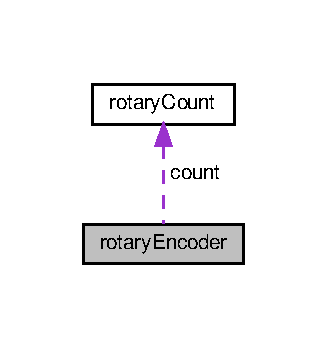
\includegraphics[width=157pt]{structrotaryEncoder__coll__graph}
\end{center}
\end{figure}
\subsection*{Public Attributes}
\begin{DoxyCompactItemize}
\item 
\mbox{\Hypertarget{structrotaryEncoder_a2512cc7964ea59e6e6d2640cb8e4c652}\label{structrotaryEncoder_a2512cc7964ea59e6e6d2640cb8e4c652}} 
\hyperlink{unionrotaryCount}{rotary\+Count} {\bfseries count}
\item 
bool \hyperlink{structrotaryEncoder_acdcf654ac998975abe284087194a57d7}{signed\+Counter}
\item 
bool \hyperlink{structrotaryEncoder_ae43c122ca1f7443eb96c728ee6021c59}{debounce\+Enable}
\item 
bool \hyperlink{structrotaryEncoder_acfd9ee89d53cb92cabb2f9e39a7d8025}{debounce\+State}
\item 
bool \hyperlink{structrotaryEncoder_a27690330142cf2a5f9e20d10b95f5dd1}{dir\+Last}
\item 
bool \hyperlink{structrotaryEncoder_a4262a64e13a2c9f3fb8c803651defde3}{alert\+Step}
\item 
bool \hyperlink{structrotaryEncoder_a99b65d81c239da055c1095045e075cf7}{use\+\_\+events}
\item 
esp\+\_\+event\+\_\+loop\+\_\+handle\+\_\+t \hyperlink{structrotaryEncoder_a1304512c915331287c57500e1f93a334}{loop}
\item 
gpio\+\_\+num\+\_\+t \hyperlink{structrotaryEncoder_ad1538a6197a4cb5f3d73c2e7ffbbdf9b}{data\+Pin\+Num}
\item 
gpio\+\_\+num\+\_\+t \hyperlink{structrotaryEncoder_ae945fca8835282470bb42d3e54f09ce7}{clock\+Pin\+Num}
\item 
\hyperlink{vl53l0x__types_8h_a273cf69d639a59973b6019625df33e30}{uint16\+\_\+t} \hyperlink{structrotaryEncoder_a790920314cd8441c59003222041bcd84}{counter\+Max}
\item 
\hyperlink{vl53l0x__types_8h_a273cf69d639a59973b6019625df33e30}{uint16\+\_\+t} \hyperlink{structrotaryEncoder_a7bf3d54d80fb253ac7fc62dee0417600}{counter\+Min}
\item 
\hyperlink{vl53l0x__types_8h_a273cf69d639a59973b6019625df33e30}{uint16\+\_\+t} \hyperlink{structrotaryEncoder_acc07389798d5ac386aef417d5999a10e}{step\+Size}
\item 
\hyperlink{vl53l0x__types_8h_a435d1572bf3f880d55459d9805097f62}{uint32\+\_\+t} \hyperlink{structrotaryEncoder_ab0862deb9b39139e677189738940dc2c}{t\+Last\+Step}
\item 
Timer\+Handle\+\_\+t \hyperlink{structrotaryEncoder_a1365b198e34d623c25c601664e07d388}{debounce\+Timer}
\item 
Task\+Handle\+\_\+t \hyperlink{structrotaryEncoder_ab489c2097bddeb8a77a52e58bf7526b7}{parent\+Task}
\end{DoxyCompactItemize}


\subsection{Member Data Documentation}
\mbox{\Hypertarget{structrotaryEncoder_a4262a64e13a2c9f3fb8c803651defde3}\label{structrotaryEncoder_a4262a64e13a2c9f3fb8c803651defde3}} 
\index{rotary\+Encoder@{rotary\+Encoder}!alert\+Step@{alert\+Step}}
\index{alert\+Step@{alert\+Step}!rotary\+Encoder@{rotary\+Encoder}}
\subsubsection{\texorpdfstring{alert\+Step}{alertStep}}
{\footnotesize\ttfamily bool rotary\+Encoder\+::alert\+Step}

$<$ last turn direction 0 -\/ c-\/clkwise, 1 -\/ clkwise \mbox{\Hypertarget{structrotaryEncoder_ae945fca8835282470bb42d3e54f09ce7}\label{structrotaryEncoder_ae945fca8835282470bb42d3e54f09ce7}} 
\index{rotary\+Encoder@{rotary\+Encoder}!clock\+Pin\+Num@{clock\+Pin\+Num}}
\index{clock\+Pin\+Num@{clock\+Pin\+Num}!rotary\+Encoder@{rotary\+Encoder}}
\subsubsection{\texorpdfstring{clock\+Pin\+Num}{clockPinNum}}
{\footnotesize\ttfamily gpio\+\_\+num\+\_\+t rotary\+Encoder\+::clock\+Pin\+Num}

$<$ data pin gpio \mbox{\Hypertarget{structrotaryEncoder_a790920314cd8441c59003222041bcd84}\label{structrotaryEncoder_a790920314cd8441c59003222041bcd84}} 
\index{rotary\+Encoder@{rotary\+Encoder}!counter\+Max@{counter\+Max}}
\index{counter\+Max@{counter\+Max}!rotary\+Encoder@{rotary\+Encoder}}
\subsubsection{\texorpdfstring{counter\+Max}{counterMax}}
{\footnotesize\ttfamily \hyperlink{vl53l0x__types_8h_a273cf69d639a59973b6019625df33e30}{uint16\+\_\+t} rotary\+Encoder\+::counter\+Max}

$<$ clock pin gpio \mbox{\Hypertarget{structrotaryEncoder_a7bf3d54d80fb253ac7fc62dee0417600}\label{structrotaryEncoder_a7bf3d54d80fb253ac7fc62dee0417600}} 
\index{rotary\+Encoder@{rotary\+Encoder}!counter\+Min@{counter\+Min}}
\index{counter\+Min@{counter\+Min}!rotary\+Encoder@{rotary\+Encoder}}
\subsubsection{\texorpdfstring{counter\+Min}{counterMin}}
{\footnotesize\ttfamily \hyperlink{vl53l0x__types_8h_a273cf69d639a59973b6019625df33e30}{uint16\+\_\+t} rotary\+Encoder\+::counter\+Min}

$<$ max counter value \mbox{\Hypertarget{structrotaryEncoder_ad1538a6197a4cb5f3d73c2e7ffbbdf9b}\label{structrotaryEncoder_ad1538a6197a4cb5f3d73c2e7ffbbdf9b}} 
\index{rotary\+Encoder@{rotary\+Encoder}!data\+Pin\+Num@{data\+Pin\+Num}}
\index{data\+Pin\+Num@{data\+Pin\+Num}!rotary\+Encoder@{rotary\+Encoder}}
\subsubsection{\texorpdfstring{data\+Pin\+Num}{dataPinNum}}
{\footnotesize\ttfamily gpio\+\_\+num\+\_\+t rotary\+Encoder\+::data\+Pin\+Num}

$<$ event loop to send events to \mbox{\Hypertarget{structrotaryEncoder_ae43c122ca1f7443eb96c728ee6021c59}\label{structrotaryEncoder_ae43c122ca1f7443eb96c728ee6021c59}} 
\index{rotary\+Encoder@{rotary\+Encoder}!debounce\+Enable@{debounce\+Enable}}
\index{debounce\+Enable@{debounce\+Enable}!rotary\+Encoder@{rotary\+Encoder}}
\subsubsection{\texorpdfstring{debounce\+Enable}{debounceEnable}}
{\footnotesize\ttfamily bool rotary\+Encoder\+::debounce\+Enable}

$<$ using signed or unsigned value \mbox{\Hypertarget{structrotaryEncoder_acfd9ee89d53cb92cabb2f9e39a7d8025}\label{structrotaryEncoder_acfd9ee89d53cb92cabb2f9e39a7d8025}} 
\index{rotary\+Encoder@{rotary\+Encoder}!debounce\+State@{debounce\+State}}
\index{debounce\+State@{debounce\+State}!rotary\+Encoder@{rotary\+Encoder}}
\subsubsection{\texorpdfstring{debounce\+State}{debounceState}}
{\footnotesize\ttfamily bool rotary\+Encoder\+::debounce\+State}

$<$ enable to button debounce \mbox{\Hypertarget{structrotaryEncoder_a1365b198e34d623c25c601664e07d388}\label{structrotaryEncoder_a1365b198e34d623c25c601664e07d388}} 
\index{rotary\+Encoder@{rotary\+Encoder}!debounce\+Timer@{debounce\+Timer}}
\index{debounce\+Timer@{debounce\+Timer}!rotary\+Encoder@{rotary\+Encoder}}
\subsubsection{\texorpdfstring{debounce\+Timer}{debounceTimer}}
{\footnotesize\ttfamily Timer\+Handle\+\_\+t rotary\+Encoder\+::debounce\+Timer}

$<$ time since the last rotary step \mbox{\Hypertarget{structrotaryEncoder_a27690330142cf2a5f9e20d10b95f5dd1}\label{structrotaryEncoder_a27690330142cf2a5f9e20d10b95f5dd1}} 
\index{rotary\+Encoder@{rotary\+Encoder}!dir\+Last@{dir\+Last}}
\index{dir\+Last@{dir\+Last}!rotary\+Encoder@{rotary\+Encoder}}
\subsubsection{\texorpdfstring{dir\+Last}{dirLast}}
{\footnotesize\ttfamily bool rotary\+Encoder\+::dir\+Last}

$<$ button debounce state \mbox{\Hypertarget{structrotaryEncoder_a1304512c915331287c57500e1f93a334}\label{structrotaryEncoder_a1304512c915331287c57500e1f93a334}} 
\index{rotary\+Encoder@{rotary\+Encoder}!loop@{loop}}
\index{loop@{loop}!rotary\+Encoder@{rotary\+Encoder}}
\subsubsection{\texorpdfstring{loop}{loop}}
{\footnotesize\ttfamily esp\+\_\+event\+\_\+loop\+\_\+handle\+\_\+t rotary\+Encoder\+::loop}

$<$ Send events on Button \& RE events \mbox{\Hypertarget{structrotaryEncoder_ab489c2097bddeb8a77a52e58bf7526b7}\label{structrotaryEncoder_ab489c2097bddeb8a77a52e58bf7526b7}} 
\index{rotary\+Encoder@{rotary\+Encoder}!parent\+Task@{parent\+Task}}
\index{parent\+Task@{parent\+Task}!rotary\+Encoder@{rotary\+Encoder}}
\subsubsection{\texorpdfstring{parent\+Task}{parentTask}}
{\footnotesize\ttfamily Task\+Handle\+\_\+t rotary\+Encoder\+::parent\+Task}

$<$ Timer for debounce \mbox{\Hypertarget{structrotaryEncoder_acdcf654ac998975abe284087194a57d7}\label{structrotaryEncoder_acdcf654ac998975abe284087194a57d7}} 
\index{rotary\+Encoder@{rotary\+Encoder}!signed\+Counter@{signed\+Counter}}
\index{signed\+Counter@{signed\+Counter}!rotary\+Encoder@{rotary\+Encoder}}
\subsubsection{\texorpdfstring{signed\+Counter}{signedCounter}}
{\footnotesize\ttfamily bool rotary\+Encoder\+::signed\+Counter}

$<$ rotary encoder counter \mbox{\Hypertarget{structrotaryEncoder_acc07389798d5ac386aef417d5999a10e}\label{structrotaryEncoder_acc07389798d5ac386aef417d5999a10e}} 
\index{rotary\+Encoder@{rotary\+Encoder}!step\+Size@{step\+Size}}
\index{step\+Size@{step\+Size}!rotary\+Encoder@{rotary\+Encoder}}
\subsubsection{\texorpdfstring{step\+Size}{stepSize}}
{\footnotesize\ttfamily \hyperlink{vl53l0x__types_8h_a273cf69d639a59973b6019625df33e30}{uint16\+\_\+t} rotary\+Encoder\+::step\+Size}

$<$ min counter value \mbox{\Hypertarget{structrotaryEncoder_ab0862deb9b39139e677189738940dc2c}\label{structrotaryEncoder_ab0862deb9b39139e677189738940dc2c}} 
\index{rotary\+Encoder@{rotary\+Encoder}!t\+Last\+Step@{t\+Last\+Step}}
\index{t\+Last\+Step@{t\+Last\+Step}!rotary\+Encoder@{rotary\+Encoder}}
\subsubsection{\texorpdfstring{t\+Last\+Step}{tLastStep}}
{\footnotesize\ttfamily \hyperlink{vl53l0x__types_8h_a435d1572bf3f880d55459d9805097f62}{uint32\+\_\+t} rotary\+Encoder\+::t\+Last\+Step}

$<$ increment/decrement size \mbox{\Hypertarget{structrotaryEncoder_a99b65d81c239da055c1095045e075cf7}\label{structrotaryEncoder_a99b65d81c239da055c1095045e075cf7}} 
\index{rotary\+Encoder@{rotary\+Encoder}!use\+\_\+events@{use\+\_\+events}}
\index{use\+\_\+events@{use\+\_\+events}!rotary\+Encoder@{rotary\+Encoder}}
\subsubsection{\texorpdfstring{use\+\_\+events}{use\_events}}
{\footnotesize\ttfamily bool rotary\+Encoder\+::use\+\_\+events}

$<$ send task notification if step changes 

The documentation for this struct was generated from the following file\+:\begin{DoxyCompactItemize}
\item 
Rotary\+Encoder\+\_\+\+Driver/Rotary\+Encoder\+\_\+\+Driver.\+h\end{DoxyCompactItemize}

\hypertarget{structrowdata__pins__t}{}\section{rowdata\+\_\+pins\+\_\+t Struct Reference}
\label{structrowdata__pins__t}\index{rowdata\+\_\+pins\+\_\+t@{rowdata\+\_\+pins\+\_\+t}}
\subsection*{Public Attributes}
\begin{DoxyCompactItemize}
\item 
\mbox{\Hypertarget{structrowdata__pins__t_af5485c290589f120ec80f689cc22f44a}\label{structrowdata__pins__t_af5485c290589f120ec80f689cc22f44a}} 
gpio\+\_\+num\+\_\+t {\bfseries D\+R0}
\item 
\mbox{\Hypertarget{structrowdata__pins__t_a7591dde9f2e804de8006a2f2f9b55bf3}\label{structrowdata__pins__t_a7591dde9f2e804de8006a2f2f9b55bf3}} 
gpio\+\_\+num\+\_\+t {\bfseries D\+R1}
\item 
\mbox{\Hypertarget{structrowdata__pins__t_a586a65c00df4a7a0b9a315cf6d5b0b34}\label{structrowdata__pins__t_a586a65c00df4a7a0b9a315cf6d5b0b34}} 
gpio\+\_\+num\+\_\+t {\bfseries D\+R2}
\item 
\mbox{\Hypertarget{structrowdata__pins__t_ad5b7edb19f02df23e152d93cfdcdc2dc}\label{structrowdata__pins__t_ad5b7edb19f02df23e152d93cfdcdc2dc}} 
gpio\+\_\+num\+\_\+t {\bfseries D\+R3}
\end{DoxyCompactItemize}


The documentation for this struct was generated from the following file\+:\begin{DoxyCompactItemize}
\item 
H\+P\+D\+L1414\+\_\+\+Driver/H\+P\+D\+L1414\+\_\+\+Driver.\+h\end{DoxyCompactItemize}

\hypertarget{structscreen__handle__t}{}\section{screen\+\_\+handle\+\_\+t Struct Reference}
\label{structscreen__handle__t}\index{screen\+\_\+handle\+\_\+t@{screen\+\_\+handle\+\_\+t}}
\subsection*{Public Attributes}
\begin{DoxyCompactItemize}
\item 
\mbox{\Hypertarget{structscreen__handle__t_ad5fa1b9c65723fe90fbaa5a96326d7ae}\label{structscreen__handle__t_ad5fa1b9c65723fe90fbaa5a96326d7ae}} 
bool {\bfseries pwr\+\_\+state}
\item 
\mbox{\Hypertarget{structscreen__handle__t_ac729f85f804e11fdaf9e6acec568deff}\label{structscreen__handle__t_ac729f85f804e11fdaf9e6acec568deff}} 
gpio\+\_\+num\+\_\+t {\bfseries rst\+\_\+pin}
\item 
\mbox{\Hypertarget{structscreen__handle__t_a4e3c5e6113a0b8eba70031cb99046bc3}\label{structscreen__handle__t_a4e3c5e6113a0b8eba70031cb99046bc3}} 
gpio\+\_\+num\+\_\+t {\bfseries cmd\+\_\+pin}
\item 
\mbox{\Hypertarget{structscreen__handle__t_a4791b6cdd636fd0990a9d83b8d840e06}\label{structscreen__handle__t_a4791b6cdd636fd0990a9d83b8d840e06}} 
\hyperlink{vl53l0x__types_8h_aba7bc1797add20fe3efdf37ced1182c5}{uint8\+\_\+t} {\bfseries spi\+\_\+bus}
\item 
\mbox{\Hypertarget{structscreen__handle__t_ac4f48c2fd6bd5cff5cebc91ed0201d92}\label{structscreen__handle__t_ac4f48c2fd6bd5cff5cebc91ed0201d92}} 
spi\+\_\+device\+\_\+handle\+\_\+t {\bfseries devhandle}
\item 
\hyperlink{vl53l0x__types_8h_a435d1572bf3f880d55459d9805097f62}{uint32\+\_\+t} \hyperlink{structscreen__handle__t_a5d83bc20f6e600a8e9133b90af8034d5}{trx\+\_\+count}
\end{DoxyCompactItemize}


\subsection{Member Data Documentation}
\mbox{\Hypertarget{structscreen__handle__t_a5d83bc20f6e600a8e9133b90af8034d5}\label{structscreen__handle__t_a5d83bc20f6e600a8e9133b90af8034d5}} 
\index{screen\+\_\+handle\+\_\+t@{screen\+\_\+handle\+\_\+t}!trx\+\_\+count@{trx\+\_\+count}}
\index{trx\+\_\+count@{trx\+\_\+count}!screen\+\_\+handle\+\_\+t@{screen\+\_\+handle\+\_\+t}}
\subsubsection{\texorpdfstring{trx\+\_\+count}{trx\_count}}
{\footnotesize\ttfamily \hyperlink{vl53l0x__types_8h_a435d1572bf3f880d55459d9805097f62}{uint32\+\_\+t} screen\+\_\+handle\+\_\+t\+::trx\+\_\+count}

$<$ screen\textquotesingle{}s spi handle 

The documentation for this struct was generated from the following file\+:\begin{DoxyCompactItemize}
\item 
S\+T7735\+\_\+\+Driver/S\+T7735\+\_\+\+Screen.\+h\end{DoxyCompactItemize}

\hypertarget{structscreen__settings__t}{}\section{screen\+\_\+settings\+\_\+t Struct Reference}
\label{structscreen__settings__t}\index{screen\+\_\+settings\+\_\+t@{screen\+\_\+settings\+\_\+t}}
\subsection*{Public Attributes}
\begin{DoxyCompactItemize}
\item 
\hyperlink{vl53l0x__types_8h_aba7bc1797add20fe3efdf37ced1182c5}{uint8\+\_\+t} \hyperlink{structscreen__settings__t_a06d597efab1bc13bc657b4ea6dae4592}{mnf\+\_\+id}
\item 
\hyperlink{vl53l0x__types_8h_aba7bc1797add20fe3efdf37ced1182c5}{uint8\+\_\+t} \hyperlink{structscreen__settings__t_a05dc3e5a9e54fdf1173dd3c9b9fbc6f4}{ver\+\_\+id}
\item 
\hyperlink{vl53l0x__types_8h_aba7bc1797add20fe3efdf37ced1182c5}{uint8\+\_\+t} \hyperlink{structscreen__settings__t_a0b6a0e2a0df6813023c86e9354a4f185}{drv\+\_\+id}
\item 
bool \hyperlink{structscreen__settings__t_aac406fcdf039a835479da26647ecf6bd}{bston}
\item 
bool \hyperlink{structscreen__settings__t_a0fb5e9d5dbc528c86d736fe19a52b843}{my}
\item 
bool \hyperlink{structscreen__settings__t_a93270669bbb6354b04cb443d569ecf28}{mx}
\item 
bool \hyperlink{structscreen__settings__t_a15540f28894b9a28bd19bbac7bf68783}{mv}
\item 
bool \hyperlink{structscreen__settings__t_adb95ada049cc88b286d64c5cee67e82b}{ml}
\item 
bool \hyperlink{structscreen__settings__t_a20c4b773bc0965d0ce9a1aa4286f1904}{rgb}
\item 
bool \hyperlink{structscreen__settings__t_a91e2e317da6bbe919f01cc9992622c9c}{mh}
\item 
\hyperlink{vl53l0x__types_8h_aba7bc1797add20fe3efdf37ced1182c5}{uint8\+\_\+t} \hyperlink{structscreen__settings__t_a40885e4438ae3b750c667132c5d5f258}{ifpf}
\item 
bool \hyperlink{structscreen__settings__t_aca5674cfa96ae81895c44eda562ba1de}{idmon}
\item 
bool \hyperlink{structscreen__settings__t_ae7cf1d9d23331e98009318749852f4a2}{ptlon}
\item 
bool \hyperlink{structscreen__settings__t_a840cbd1ac22e878d2828d8780daccc2c}{slpout}
\item 
bool \hyperlink{structscreen__settings__t_aaf1cf50e0a9396996091156f0b7a3bd3}{noron}
\item 
bool \hyperlink{structscreen__settings__t_a9d13034a607f38a182223f8fcc6dada1}{invon}
\item 
bool \hyperlink{structscreen__settings__t_a8fd1aa43e1400e9376ba9f1e66994a5c}{dison}
\item 
\hyperlink{vl53l0x__types_8h_aba7bc1797add20fe3efdf37ced1182c5}{uint8\+\_\+t} \hyperlink{structscreen__settings__t_a696f0baa16234456867bacc806b59537}{gcs}
\item 
bool \hyperlink{structscreen__settings__t_a4c6ed6c63c228d7f9e68a9627d43b259}{telon}
\item 
bool \hyperlink{structscreen__settings__t_ace00804e6bf6c200c79a0746ba6e462f}{telom}
\end{DoxyCompactItemize}


\subsection{Member Data Documentation}
\mbox{\Hypertarget{structscreen__settings__t_aac406fcdf039a835479da26647ecf6bd}\label{structscreen__settings__t_aac406fcdf039a835479da26647ecf6bd}} 
\index{screen\+\_\+settings\+\_\+t@{screen\+\_\+settings\+\_\+t}!bston@{bston}}
\index{bston@{bston}!screen\+\_\+settings\+\_\+t@{screen\+\_\+settings\+\_\+t}}
\subsubsection{\texorpdfstring{bston}{bston}}
{\footnotesize\ttfamily bool screen\+\_\+settings\+\_\+t\+::bston}

booster voltage status \mbox{\Hypertarget{structscreen__settings__t_a8fd1aa43e1400e9376ba9f1e66994a5c}\label{structscreen__settings__t_a8fd1aa43e1400e9376ba9f1e66994a5c}} 
\index{screen\+\_\+settings\+\_\+t@{screen\+\_\+settings\+\_\+t}!dison@{dison}}
\index{dison@{dison}!screen\+\_\+settings\+\_\+t@{screen\+\_\+settings\+\_\+t}}
\subsubsection{\texorpdfstring{dison}{dison}}
{\footnotesize\ttfamily bool screen\+\_\+settings\+\_\+t\+::dison}

display on/off \mbox{\Hypertarget{structscreen__settings__t_a0b6a0e2a0df6813023c86e9354a4f185}\label{structscreen__settings__t_a0b6a0e2a0df6813023c86e9354a4f185}} 
\index{screen\+\_\+settings\+\_\+t@{screen\+\_\+settings\+\_\+t}!drv\+\_\+id@{drv\+\_\+id}}
\index{drv\+\_\+id@{drv\+\_\+id}!screen\+\_\+settings\+\_\+t@{screen\+\_\+settings\+\_\+t}}
\subsubsection{\texorpdfstring{drv\+\_\+id}{drv\_id}}
{\footnotesize\ttfamily \hyperlink{vl53l0x__types_8h_aba7bc1797add20fe3efdf37ced1182c5}{uint8\+\_\+t} screen\+\_\+settings\+\_\+t\+::drv\+\_\+id}

driver id \char`\"{}\char`\"{} \mbox{\Hypertarget{structscreen__settings__t_a696f0baa16234456867bacc806b59537}\label{structscreen__settings__t_a696f0baa16234456867bacc806b59537}} 
\index{screen\+\_\+settings\+\_\+t@{screen\+\_\+settings\+\_\+t}!gcs@{gcs}}
\index{gcs@{gcs}!screen\+\_\+settings\+\_\+t@{screen\+\_\+settings\+\_\+t}}
\subsubsection{\texorpdfstring{gcs}{gcs}}
{\footnotesize\ttfamily \hyperlink{vl53l0x__types_8h_aba7bc1797add20fe3efdf37ced1182c5}{uint8\+\_\+t} screen\+\_\+settings\+\_\+t\+::gcs}

gamma curve selection \mbox{\Hypertarget{structscreen__settings__t_aca5674cfa96ae81895c44eda562ba1de}\label{structscreen__settings__t_aca5674cfa96ae81895c44eda562ba1de}} 
\index{screen\+\_\+settings\+\_\+t@{screen\+\_\+settings\+\_\+t}!idmon@{idmon}}
\index{idmon@{idmon}!screen\+\_\+settings\+\_\+t@{screen\+\_\+settings\+\_\+t}}
\subsubsection{\texorpdfstring{idmon}{idmon}}
{\footnotesize\ttfamily bool screen\+\_\+settings\+\_\+t\+::idmon}

idle mode \mbox{\Hypertarget{structscreen__settings__t_a40885e4438ae3b750c667132c5d5f258}\label{structscreen__settings__t_a40885e4438ae3b750c667132c5d5f258}} 
\index{screen\+\_\+settings\+\_\+t@{screen\+\_\+settings\+\_\+t}!ifpf@{ifpf}}
\index{ifpf@{ifpf}!screen\+\_\+settings\+\_\+t@{screen\+\_\+settings\+\_\+t}}
\subsubsection{\texorpdfstring{ifpf}{ifpf}}
{\footnotesize\ttfamily \hyperlink{vl53l0x__types_8h_aba7bc1797add20fe3efdf37ced1182c5}{uint8\+\_\+t} screen\+\_\+settings\+\_\+t\+::ifpf}

interface color puxel format def \mbox{\Hypertarget{structscreen__settings__t_a9d13034a607f38a182223f8fcc6dada1}\label{structscreen__settings__t_a9d13034a607f38a182223f8fcc6dada1}} 
\index{screen\+\_\+settings\+\_\+t@{screen\+\_\+settings\+\_\+t}!invon@{invon}}
\index{invon@{invon}!screen\+\_\+settings\+\_\+t@{screen\+\_\+settings\+\_\+t}}
\subsubsection{\texorpdfstring{invon}{invon}}
{\footnotesize\ttfamily bool screen\+\_\+settings\+\_\+t\+::invon}

inverted mode \mbox{\Hypertarget{structscreen__settings__t_a91e2e317da6bbe919f01cc9992622c9c}\label{structscreen__settings__t_a91e2e317da6bbe919f01cc9992622c9c}} 
\index{screen\+\_\+settings\+\_\+t@{screen\+\_\+settings\+\_\+t}!mh@{mh}}
\index{mh@{mh}!screen\+\_\+settings\+\_\+t@{screen\+\_\+settings\+\_\+t}}
\subsubsection{\texorpdfstring{mh}{mh}}
{\footnotesize\ttfamily bool screen\+\_\+settings\+\_\+t\+::mh}

horizontal order \mbox{\Hypertarget{structscreen__settings__t_adb95ada049cc88b286d64c5cee67e82b}\label{structscreen__settings__t_adb95ada049cc88b286d64c5cee67e82b}} 
\index{screen\+\_\+settings\+\_\+t@{screen\+\_\+settings\+\_\+t}!ml@{ml}}
\index{ml@{ml}!screen\+\_\+settings\+\_\+t@{screen\+\_\+settings\+\_\+t}}
\subsubsection{\texorpdfstring{ml}{ml}}
{\footnotesize\ttfamily bool screen\+\_\+settings\+\_\+t\+::ml}

scan address order \mbox{\Hypertarget{structscreen__settings__t_a06d597efab1bc13bc657b4ea6dae4592}\label{structscreen__settings__t_a06d597efab1bc13bc657b4ea6dae4592}} 
\index{screen\+\_\+settings\+\_\+t@{screen\+\_\+settings\+\_\+t}!mnf\+\_\+id@{mnf\+\_\+id}}
\index{mnf\+\_\+id@{mnf\+\_\+id}!screen\+\_\+settings\+\_\+t@{screen\+\_\+settings\+\_\+t}}
\subsubsection{\texorpdfstring{mnf\+\_\+id}{mnf\_id}}
{\footnotesize\ttfamily \hyperlink{vl53l0x__types_8h_aba7bc1797add20fe3efdf37ced1182c5}{uint8\+\_\+t} screen\+\_\+settings\+\_\+t\+::mnf\+\_\+id}

manufacturer\textquotesingle{}s id (0x5c) \mbox{\Hypertarget{structscreen__settings__t_a15540f28894b9a28bd19bbac7bf68783}\label{structscreen__settings__t_a15540f28894b9a28bd19bbac7bf68783}} 
\index{screen\+\_\+settings\+\_\+t@{screen\+\_\+settings\+\_\+t}!mv@{mv}}
\index{mv@{mv}!screen\+\_\+settings\+\_\+t@{screen\+\_\+settings\+\_\+t}}
\subsubsection{\texorpdfstring{mv}{mv}}
{\footnotesize\ttfamily bool screen\+\_\+settings\+\_\+t\+::mv}

row/col exchange \mbox{\Hypertarget{structscreen__settings__t_a93270669bbb6354b04cb443d569ecf28}\label{structscreen__settings__t_a93270669bbb6354b04cb443d569ecf28}} 
\index{screen\+\_\+settings\+\_\+t@{screen\+\_\+settings\+\_\+t}!mx@{mx}}
\index{mx@{mx}!screen\+\_\+settings\+\_\+t@{screen\+\_\+settings\+\_\+t}}
\subsubsection{\texorpdfstring{mx}{mx}}
{\footnotesize\ttfamily bool screen\+\_\+settings\+\_\+t\+::mx}

col address order \mbox{\Hypertarget{structscreen__settings__t_a0fb5e9d5dbc528c86d736fe19a52b843}\label{structscreen__settings__t_a0fb5e9d5dbc528c86d736fe19a52b843}} 
\index{screen\+\_\+settings\+\_\+t@{screen\+\_\+settings\+\_\+t}!my@{my}}
\index{my@{my}!screen\+\_\+settings\+\_\+t@{screen\+\_\+settings\+\_\+t}}
\subsubsection{\texorpdfstring{my}{my}}
{\footnotesize\ttfamily bool screen\+\_\+settings\+\_\+t\+::my}

row address order \mbox{\Hypertarget{structscreen__settings__t_aaf1cf50e0a9396996091156f0b7a3bd3}\label{structscreen__settings__t_aaf1cf50e0a9396996091156f0b7a3bd3}} 
\index{screen\+\_\+settings\+\_\+t@{screen\+\_\+settings\+\_\+t}!noron@{noron}}
\index{noron@{noron}!screen\+\_\+settings\+\_\+t@{screen\+\_\+settings\+\_\+t}}
\subsubsection{\texorpdfstring{noron}{noron}}
{\footnotesize\ttfamily bool screen\+\_\+settings\+\_\+t\+::noron}

normal mode \mbox{\Hypertarget{structscreen__settings__t_ae7cf1d9d23331e98009318749852f4a2}\label{structscreen__settings__t_ae7cf1d9d23331e98009318749852f4a2}} 
\index{screen\+\_\+settings\+\_\+t@{screen\+\_\+settings\+\_\+t}!ptlon@{ptlon}}
\index{ptlon@{ptlon}!screen\+\_\+settings\+\_\+t@{screen\+\_\+settings\+\_\+t}}
\subsubsection{\texorpdfstring{ptlon}{ptlon}}
{\footnotesize\ttfamily bool screen\+\_\+settings\+\_\+t\+::ptlon}

paartial mode \mbox{\Hypertarget{structscreen__settings__t_a20c4b773bc0965d0ce9a1aa4286f1904}\label{structscreen__settings__t_a20c4b773bc0965d0ce9a1aa4286f1904}} 
\index{screen\+\_\+settings\+\_\+t@{screen\+\_\+settings\+\_\+t}!rgb@{rgb}}
\index{rgb@{rgb}!screen\+\_\+settings\+\_\+t@{screen\+\_\+settings\+\_\+t}}
\subsubsection{\texorpdfstring{rgb}{rgb}}
{\footnotesize\ttfamily bool screen\+\_\+settings\+\_\+t\+::rgb}

rgb order \mbox{\Hypertarget{structscreen__settings__t_a840cbd1ac22e878d2828d8780daccc2c}\label{structscreen__settings__t_a840cbd1ac22e878d2828d8780daccc2c}} 
\index{screen\+\_\+settings\+\_\+t@{screen\+\_\+settings\+\_\+t}!slpout@{slpout}}
\index{slpout@{slpout}!screen\+\_\+settings\+\_\+t@{screen\+\_\+settings\+\_\+t}}
\subsubsection{\texorpdfstring{slpout}{slpout}}
{\footnotesize\ttfamily bool screen\+\_\+settings\+\_\+t\+::slpout}

sleep out/in \mbox{\Hypertarget{structscreen__settings__t_ace00804e6bf6c200c79a0746ba6e462f}\label{structscreen__settings__t_ace00804e6bf6c200c79a0746ba6e462f}} 
\index{screen\+\_\+settings\+\_\+t@{screen\+\_\+settings\+\_\+t}!telom@{telom}}
\index{telom@{telom}!screen\+\_\+settings\+\_\+t@{screen\+\_\+settings\+\_\+t}}
\subsubsection{\texorpdfstring{telom}{telom}}
{\footnotesize\ttfamily bool screen\+\_\+settings\+\_\+t\+::telom}

tearing effect mode \mbox{\Hypertarget{structscreen__settings__t_a4c6ed6c63c228d7f9e68a9627d43b259}\label{structscreen__settings__t_a4c6ed6c63c228d7f9e68a9627d43b259}} 
\index{screen\+\_\+settings\+\_\+t@{screen\+\_\+settings\+\_\+t}!telon@{telon}}
\index{telon@{telon}!screen\+\_\+settings\+\_\+t@{screen\+\_\+settings\+\_\+t}}
\subsubsection{\texorpdfstring{telon}{telon}}
{\footnotesize\ttfamily bool screen\+\_\+settings\+\_\+t\+::telon}

tearing effect on/off \mbox{\Hypertarget{structscreen__settings__t_a05dc3e5a9e54fdf1173dd3c9b9fbc6f4}\label{structscreen__settings__t_a05dc3e5a9e54fdf1173dd3c9b9fbc6f4}} 
\index{screen\+\_\+settings\+\_\+t@{screen\+\_\+settings\+\_\+t}!ver\+\_\+id@{ver\+\_\+id}}
\index{ver\+\_\+id@{ver\+\_\+id}!screen\+\_\+settings\+\_\+t@{screen\+\_\+settings\+\_\+t}}
\subsubsection{\texorpdfstring{ver\+\_\+id}{ver\_id}}
{\footnotesize\ttfamily \hyperlink{vl53l0x__types_8h_aba7bc1797add20fe3efdf37ced1182c5}{uint8\+\_\+t} screen\+\_\+settings\+\_\+t\+::ver\+\_\+id}

version id \char`\"{}\char`\"{} 

The documentation for this struct was generated from the following file\+:\begin{DoxyCompactItemize}
\item 
S\+T7735\+\_\+\+Driver/S\+T7735\+\_\+\+Screen.\+h\end{DoxyCompactItemize}

\hypertarget{structscreen__transaction__t}{}\section{screen\+\_\+transaction\+\_\+t Struct Reference}
\label{structscreen__transaction__t}\index{screen\+\_\+transaction\+\_\+t@{screen\+\_\+transaction\+\_\+t}}
\subsection*{Public Attributes}
\begin{DoxyCompactItemize}
\item 
\mbox{\Hypertarget{structscreen__transaction__t_af29c3c70326c33692c8f1aab31170093}\label{structscreen__transaction__t_af29c3c70326c33692c8f1aab31170093}} 
bool {\bfseries mode}
\item 
\hyperlink{vl53l0x__types_8h_aba7bc1797add20fe3efdf37ced1182c5}{uint8\+\_\+t} $\ast$ \hyperlink{structscreen__transaction__t_ad61b850a61304532df31ac1699b71911}{send}
\item 
\hyperlink{vl53l0x__types_8h_aba7bc1797add20fe3efdf37ced1182c5}{uint8\+\_\+t} $\ast$ \hyperlink{structscreen__transaction__t_ac00eeb10dbec656aeb6d4cd81bc4533c}{recv}
\item 
\hyperlink{vl53l0x__types_8h_a273cf69d639a59973b6019625df33e30}{uint16\+\_\+t} \hyperlink{structscreen__transaction__t_ade485ce9cfd695b682aa0827ef8dd8ce}{s\+\_\+len}
\item 
\hyperlink{vl53l0x__types_8h_a273cf69d639a59973b6019625df33e30}{uint16\+\_\+t} \hyperlink{structscreen__transaction__t_a5f7bed33270626b40a9e44bbdc73c7e0}{r\+\_\+len}
\item 
esp\+\_\+err\+\_\+t \hyperlink{structscreen__transaction__t_a1ee2e2ae378bc746fb656a0d5ec31d8b}{trx\+\_\+status}
\end{DoxyCompactItemize}


\subsection{Member Data Documentation}
\mbox{\Hypertarget{structscreen__transaction__t_a5f7bed33270626b40a9e44bbdc73c7e0}\label{structscreen__transaction__t_a5f7bed33270626b40a9e44bbdc73c7e0}} 
\index{screen\+\_\+transaction\+\_\+t@{screen\+\_\+transaction\+\_\+t}!r\+\_\+len@{r\+\_\+len}}
\index{r\+\_\+len@{r\+\_\+len}!screen\+\_\+transaction\+\_\+t@{screen\+\_\+transaction\+\_\+t}}
\subsubsection{\texorpdfstring{r\+\_\+len}{r\_len}}
{\footnotesize\ttfamily \hyperlink{vl53l0x__types_8h_a273cf69d639a59973b6019625df33e30}{uint16\+\_\+t} screen\+\_\+transaction\+\_\+t\+::r\+\_\+len}

$<$ send length \mbox{\Hypertarget{structscreen__transaction__t_ac00eeb10dbec656aeb6d4cd81bc4533c}\label{structscreen__transaction__t_ac00eeb10dbec656aeb6d4cd81bc4533c}} 
\index{screen\+\_\+transaction\+\_\+t@{screen\+\_\+transaction\+\_\+t}!recv@{recv}}
\index{recv@{recv}!screen\+\_\+transaction\+\_\+t@{screen\+\_\+transaction\+\_\+t}}
\subsubsection{\texorpdfstring{recv}{recv}}
{\footnotesize\ttfamily \hyperlink{vl53l0x__types_8h_aba7bc1797add20fe3efdf37ced1182c5}{uint8\+\_\+t}$\ast$ screen\+\_\+transaction\+\_\+t\+::recv}

$<$ pointer to send buffer \mbox{\Hypertarget{structscreen__transaction__t_ade485ce9cfd695b682aa0827ef8dd8ce}\label{structscreen__transaction__t_ade485ce9cfd695b682aa0827ef8dd8ce}} 
\index{screen\+\_\+transaction\+\_\+t@{screen\+\_\+transaction\+\_\+t}!s\+\_\+len@{s\+\_\+len}}
\index{s\+\_\+len@{s\+\_\+len}!screen\+\_\+transaction\+\_\+t@{screen\+\_\+transaction\+\_\+t}}
\subsubsection{\texorpdfstring{s\+\_\+len}{s\_len}}
{\footnotesize\ttfamily \hyperlink{vl53l0x__types_8h_a273cf69d639a59973b6019625df33e30}{uint16\+\_\+t} screen\+\_\+transaction\+\_\+t\+::s\+\_\+len}

$<$ pointer to recv buffer \mbox{\Hypertarget{structscreen__transaction__t_ad61b850a61304532df31ac1699b71911}\label{structscreen__transaction__t_ad61b850a61304532df31ac1699b71911}} 
\index{screen\+\_\+transaction\+\_\+t@{screen\+\_\+transaction\+\_\+t}!send@{send}}
\index{send@{send}!screen\+\_\+transaction\+\_\+t@{screen\+\_\+transaction\+\_\+t}}
\subsubsection{\texorpdfstring{send}{send}}
{\footnotesize\ttfamily \hyperlink{vl53l0x__types_8h_aba7bc1797add20fe3efdf37ced1182c5}{uint8\+\_\+t}$\ast$ screen\+\_\+transaction\+\_\+t\+::send}

$<$ 0 -\/ command write 1 -\/ memory write \mbox{\Hypertarget{structscreen__transaction__t_a1ee2e2ae378bc746fb656a0d5ec31d8b}\label{structscreen__transaction__t_a1ee2e2ae378bc746fb656a0d5ec31d8b}} 
\index{screen\+\_\+transaction\+\_\+t@{screen\+\_\+transaction\+\_\+t}!trx\+\_\+status@{trx\+\_\+status}}
\index{trx\+\_\+status@{trx\+\_\+status}!screen\+\_\+transaction\+\_\+t@{screen\+\_\+transaction\+\_\+t}}
\subsubsection{\texorpdfstring{trx\+\_\+status}{trx\_status}}
{\footnotesize\ttfamily esp\+\_\+err\+\_\+t screen\+\_\+transaction\+\_\+t\+::trx\+\_\+status}

$<$ recv length 

The documentation for this struct was generated from the following file\+:\begin{DoxyCompactItemize}
\item 
S\+T7735\+\_\+\+Driver/S\+T7735\+\_\+\+Screen.\+h\end{DoxyCompactItemize}

\hypertarget{structsim800__init}{}\section{sim800\+\_\+init Struct Reference}
\label{structsim800__init}\index{sim800\+\_\+init@{sim800\+\_\+init}}
\subsection*{Public Attributes}
\begin{DoxyCompactItemize}
\item 
\mbox{\Hypertarget{structsim800__init_a5c7eab722aeb88a93b05ddd8c162431f}\label{structsim800__init_a5c7eab722aeb88a93b05ddd8c162431f}} 
uart\+\_\+port\+\_\+t {\bfseries port}
\item 
\mbox{\Hypertarget{structsim800__init_a01e1cb1d91adbe63ed30578c0e12f529}\label{structsim800__init_a01e1cb1d91adbe63ed30578c0e12f529}} 
gpio\+\_\+num\+\_\+t {\bfseries tx}
\item 
\mbox{\Hypertarget{structsim800__init_a2e1082415bb5e54ff5c5e6bb6d7bc31c}\label{structsim800__init_a2e1082415bb5e54ff5c5e6bb6d7bc31c}} 
gpio\+\_\+num\+\_\+t {\bfseries rx}
\end{DoxyCompactItemize}


The documentation for this struct was generated from the following file\+:\begin{DoxyCompactItemize}
\item 
Sim800\+L\+\_\+\+Driver/S\+I\+M800\+L\+\_\+\+Driver.\+h\end{DoxyCompactItemize}

\hypertarget{structSIM800L__Driver}{}\section{S\+I\+M800\+L\+\_\+\+Driver Struct Reference}
\label{structSIM800L__Driver}\index{S\+I\+M800\+L\+\_\+\+Driver@{S\+I\+M800\+L\+\_\+\+Driver}}
\subsection*{Public Attributes}
\begin{DoxyCompactItemize}
\item 
\mbox{\Hypertarget{structSIM800L__Driver_ad562f9593d1258b675ef1903d2d27e49}\label{structSIM800L__Driver_ad562f9593d1258b675ef1903d2d27e49}} 
gpio\+\_\+num\+\_\+t {\bfseries tx}
\item 
\mbox{\Hypertarget{structSIM800L__Driver_a4a62b8582717ae3e175b5680be23974f}\label{structSIM800L__Driver_a4a62b8582717ae3e175b5680be23974f}} 
gpio\+\_\+num\+\_\+t {\bfseries rx}
\item 
\mbox{\Hypertarget{structSIM800L__Driver_a034225556bcf211f3a32a48280204068}\label{structSIM800L__Driver_a034225556bcf211f3a32a48280204068}} 
uart\+\_\+port\+\_\+t {\bfseries port}
\end{DoxyCompactItemize}


The documentation for this struct was generated from the following file\+:\begin{DoxyCompactItemize}
\item 
Sim800\+L\+\_\+\+Driver/S\+I\+M800\+L\+\_\+\+Driver.\+h\end{DoxyCompactItemize}

\hypertarget{structSimpleAnalogInit}{}\section{Simple\+Analog\+Init Struct Reference}
\label{structSimpleAnalogInit}\index{Simple\+Analog\+Init@{Simple\+Analog\+Init}}
\subsection*{Public Attributes}
\begin{DoxyCompactItemize}
\item 
\mbox{\Hypertarget{structSimpleAnalogInit_aba1d26961c84735ef70791099d57a45c}\label{structSimpleAnalogInit_aba1d26961c84735ef70791099d57a45c}} 
adc\+\_\+channel\+\_\+t {\bfseries a\+\_\+chan}
\item 
\mbox{\Hypertarget{structSimpleAnalogInit_a5e0751b696f654596d39562201f61de0}\label{structSimpleAnalogInit_a5e0751b696f654596d39562201f61de0}} 
adc\+\_\+channel\+\_\+t {\bfseries b\+\_\+chan}
\item 
\mbox{\Hypertarget{structSimpleAnalogInit_a771dab29755bc3ca2de31c3940fb5bf1}\label{structSimpleAnalogInit_a771dab29755bc3ca2de31c3940fb5bf1}} 
adc\+\_\+channel\+\_\+t {\bfseries c\+\_\+chan}
\item 
\mbox{\Hypertarget{structSimpleAnalogInit_a882561096789eb3e23cc73fc5f897837}\label{structSimpleAnalogInit_a882561096789eb3e23cc73fc5f897837}} 
adc\+\_\+bits\+\_\+width\+\_\+t {\bfseries width}
\item 
\mbox{\Hypertarget{structSimpleAnalogInit_ab42042f514c5fd66867f71b47c6322f1}\label{structSimpleAnalogInit_ab42042f514c5fd66867f71b47c6322f1}} 
adc\+\_\+atten\+\_\+t {\bfseries atten}
\end{DoxyCompactItemize}


The documentation for this struct was generated from the following file\+:\begin{DoxyCompactItemize}
\item 
Utils/Simple\+Analog\+Input.\+h\end{DoxyCompactItemize}

\hypertarget{structSimpleAnalogInput}{}\section{Simple\+Analog\+Input Struct Reference}
\label{structSimpleAnalogInput}\index{Simple\+Analog\+Input@{Simple\+Analog\+Input}}
\subsection*{Public Attributes}
\begin{DoxyCompactItemize}
\item 
\mbox{\Hypertarget{structSimpleAnalogInput_ab4596b9b21f9cd89606fac1102ed249f}\label{structSimpleAnalogInput_ab4596b9b21f9cd89606fac1102ed249f}} 
adc\+\_\+channel\+\_\+t {\bfseries adc\+\_\+channel\+\_\+a}
\item 
\mbox{\Hypertarget{structSimpleAnalogInput_a864f945ccc8f2ad67753a5e728d4b1f8}\label{structSimpleAnalogInput_a864f945ccc8f2ad67753a5e728d4b1f8}} 
adc\+\_\+channel\+\_\+t {\bfseries adc\+\_\+channel\+\_\+b}
\item 
\mbox{\Hypertarget{structSimpleAnalogInput_ae9e7e8d6db10cdb900d198681874b665}\label{structSimpleAnalogInput_ae9e7e8d6db10cdb900d198681874b665}} 
adc\+\_\+channel\+\_\+t {\bfseries adc\+\_\+channel\+\_\+c}
\item 
\mbox{\Hypertarget{structSimpleAnalogInput_a2895a4b62f46018b80cfa6aaf8672f91}\label{structSimpleAnalogInput_a2895a4b62f46018b80cfa6aaf8672f91}} 
adc\+\_\+bits\+\_\+width\+\_\+t {\bfseries width}
\item 
\mbox{\Hypertarget{structSimpleAnalogInput_a16601666577f31df97d9f6ebfcdd8871}\label{structSimpleAnalogInput_a16601666577f31df97d9f6ebfcdd8871}} 
adc\+\_\+atten\+\_\+t {\bfseries atten}
\item 
\mbox{\Hypertarget{structSimpleAnalogInput_adb0d4af6d29346a005e4ac8daaf57ec0}\label{structSimpleAnalogInput_adb0d4af6d29346a005e4ac8daaf57ec0}} 
\hyperlink{vl53l0x__types_8h_a435d1572bf3f880d55459d9805097f62}{uint32\+\_\+t} {\bfseries a\+\_\+last}
\item 
\mbox{\Hypertarget{structSimpleAnalogInput_ad707ed320a834b76c95f090a56ac322b}\label{structSimpleAnalogInput_ad707ed320a834b76c95f090a56ac322b}} 
\hyperlink{vl53l0x__types_8h_a435d1572bf3f880d55459d9805097f62}{uint32\+\_\+t} {\bfseries b\+\_\+last}
\item 
\mbox{\Hypertarget{structSimpleAnalogInput_a543707372dbec10860d913c118a6c031}\label{structSimpleAnalogInput_a543707372dbec10860d913c118a6c031}} 
\hyperlink{vl53l0x__types_8h_a435d1572bf3f880d55459d9805097f62}{uint32\+\_\+t} {\bfseries c\+\_\+last}
\item 
\mbox{\Hypertarget{structSimpleAnalogInput_a25bc1785a9847620bf8e6802c07913f4}\label{structSimpleAnalogInput_a25bc1785a9847620bf8e6802c07913f4}} 
\hyperlink{vl53l0x__types_8h_aba7bc1797add20fe3efdf37ced1182c5}{uint8\+\_\+t} {\bfseries delta\+\_\+thresh}
\end{DoxyCompactItemize}


The documentation for this struct was generated from the following file\+:\begin{DoxyCompactItemize}
\item 
Utils/Simple\+Analog\+Input.\+h\end{DoxyCompactItemize}

\hypertarget{structssd1306__handle}{}\section{ssd1306\+\_\+handle Struct Reference}
\label{structssd1306__handle}\index{ssd1306\+\_\+handle@{ssd1306\+\_\+handle}}
\subsection*{Public Attributes}
\begin{DoxyCompactItemize}
\item 
\mbox{\Hypertarget{structssd1306__handle_afd785b447779c6886dedcf4e330711e9}\label{structssd1306__handle_afd785b447779c6886dedcf4e330711e9}} 
\hyperlink{vl53l0x__types_8h_aba7bc1797add20fe3efdf37ced1182c5}{uint8\+\_\+t} {\bfseries bus}
\item 
\mbox{\Hypertarget{structssd1306__handle_a83a760e0804a4adb109b229c1f7d9378}\label{structssd1306__handle_a83a760e0804a4adb109b229c1f7d9378}} 
\hyperlink{vl53l0x__types_8h_aba7bc1797add20fe3efdf37ced1182c5}{uint8\+\_\+t} {\bfseries dev\+\_\+addr}
\item 
\mbox{\Hypertarget{structssd1306__handle_aca44aad8cf6f7cb43c8159235cdfcc4f}\label{structssd1306__handle_aca44aad8cf6f7cb43c8159235cdfcc4f}} 
\hyperlink{vl53l0x__types_8h_a273cf69d639a59973b6019625df33e30}{uint16\+\_\+t} {\bfseries pixel\+\_\+width}
\item 
\mbox{\Hypertarget{structssd1306__handle_ae2db43163af0355b4b2aadda31bd63c9}\label{structssd1306__handle_ae2db43163af0355b4b2aadda31bd63c9}} 
\hyperlink{vl53l0x__types_8h_a273cf69d639a59973b6019625df33e30}{uint16\+\_\+t} {\bfseries pixel\+\_\+height}
\item 
\mbox{\Hypertarget{structssd1306__handle_aa56de185167e9baedba382dce09d54d6}\label{structssd1306__handle_aa56de185167e9baedba382dce09d54d6}} 
\hyperlink{vl53l0x__types_8h_aba7bc1797add20fe3efdf37ced1182c5}{uint8\+\_\+t} {\bfseries current\+\_\+page}
\item 
\mbox{\Hypertarget{structssd1306__handle_ae35c72bfb567589ced15cf1ae71fe8e2}\label{structssd1306__handle_ae35c72bfb567589ced15cf1ae71fe8e2}} 
char {\bfseries text} \mbox{[}S\+S\+D\+\_\+\+M\+A\+X\+\_\+\+S\+T\+R\+L\+EN\mbox{]}
\item 
\mbox{\Hypertarget{structssd1306__handle_ac68325b273962b629ef12aa9ec066848}\label{structssd1306__handle_ac68325b273962b629ef12aa9ec066848}} 
\hyperlink{vl53l0x__types_8h_a273cf69d639a59973b6019625df33e30}{uint16\+\_\+t} {\bfseries text\+\_\+len}
\item 
\hyperlink{vl53l0x__types_8h_aba7bc1797add20fe3efdf37ced1182c5}{uint8\+\_\+t} \hyperlink{structssd1306__handle_a335175b6d6dfae547935246bc1ba6fef}{orientation}
\item 
\mbox{\Hypertarget{structssd1306__handle_a295dcfb0e099238228d3cd4ac4d06444}\label{structssd1306__handle_a295dcfb0e099238228d3cd4ac4d06444}} 
bool {\bfseries active}
\item 
\mbox{\Hypertarget{structssd1306__handle_af0ffd518fb6dda992a364a3f8df0831d}\label{structssd1306__handle_af0ffd518fb6dda992a364a3f8df0831d}} 
\hyperlink{vl53l0x__types_8h_aba7bc1797add20fe3efdf37ced1182c5}{uint8\+\_\+t} {\bfseries scroll\+\_\+speed}
\item 
\mbox{\Hypertarget{structssd1306__handle_aa3ac863755956825b70806189bd19305}\label{structssd1306__handle_aa3ac863755956825b70806189bd19305}} 
bool {\bfseries is\+\_\+scrolling}
\item 
\mbox{\Hypertarget{structssd1306__handle_abec5b63e2bbef8942051d3a76b0fd3f5}\label{structssd1306__handle_abec5b63e2bbef8942051d3a76b0fd3f5}} 
\hyperlink{vl53l0x__types_8h_aba7bc1797add20fe3efdf37ced1182c5}{uint8\+\_\+t} {\bfseries contrast}
\item 
\mbox{\Hypertarget{structssd1306__handle_a40bd775f1f513f848e481c40e60e80ac}\label{structssd1306__handle_a40bd775f1f513f848e481c40e60e80ac}} 
Timer\+Handle\+\_\+t {\bfseries timer}
\item 
\mbox{\Hypertarget{structssd1306__handle_a2d44b261112935120dd465248bf85a0b}\label{structssd1306__handle_a2d44b261112935120dd465248bf85a0b}} 
Task\+Handle\+\_\+t {\bfseries task\+\_\+handle}
\end{DoxyCompactItemize}


\subsection{Member Data Documentation}
\mbox{\Hypertarget{structssd1306__handle_a335175b6d6dfae547935246bc1ba6fef}\label{structssd1306__handle_a335175b6d6dfae547935246bc1ba6fef}} 
\index{ssd1306\+\_\+handle@{ssd1306\+\_\+handle}!orientation@{orientation}}
\index{orientation@{orientation}!ssd1306\+\_\+handle@{ssd1306\+\_\+handle}}
\subsubsection{\texorpdfstring{orientation}{orientation}}
{\footnotesize\ttfamily \hyperlink{vl53l0x__types_8h_aba7bc1797add20fe3efdf37ced1182c5}{uint8\+\_\+t} ssd1306\+\_\+handle\+::orientation}

0, one way, 1$>$ other way 

The documentation for this struct was generated from the following file\+:\begin{DoxyCompactItemize}
\item 
S\+S\+D1306\+\_\+\+Driver/S\+S\+D1306\+\_\+\+Driver.\+h\end{DoxyCompactItemize}

\hypertarget{structssd1306__init}{}\section{ssd1306\+\_\+init Struct Reference}
\label{structssd1306__init}\index{ssd1306\+\_\+init@{ssd1306\+\_\+init}}
\subsection*{Public Attributes}
\begin{DoxyCompactItemize}
\item 
\mbox{\Hypertarget{structssd1306__init_aad496fa83a8fb52d4fbe0963110f9f42}\label{structssd1306__init_aad496fa83a8fb52d4fbe0963110f9f42}} 
\hyperlink{vl53l0x__types_8h_aba7bc1797add20fe3efdf37ced1182c5}{uint8\+\_\+t} {\bfseries i2c\+\_\+bus}
\item 
\mbox{\Hypertarget{structssd1306__init_ac81c6354f84be18b4dbe48ee6d1c2ce5}\label{structssd1306__init_ac81c6354f84be18b4dbe48ee6d1c2ce5}} 
\hyperlink{vl53l0x__types_8h_aba7bc1797add20fe3efdf37ced1182c5}{uint8\+\_\+t} {\bfseries i2c\+\_\+addr}
\end{DoxyCompactItemize}


The documentation for this struct was generated from the following file\+:\begin{DoxyCompactItemize}
\item 
S\+S\+D1306\+\_\+\+Driver/S\+S\+D1306\+\_\+\+Driver.\+h\end{DoxyCompactItemize}

\hypertarget{structst7735__init}{}\section{st7735\+\_\+init Struct Reference}
\label{structst7735__init}\index{st7735\+\_\+init@{st7735\+\_\+init}}
\subsection*{Public Attributes}
\begin{DoxyCompactItemize}
\item 
\mbox{\Hypertarget{structst7735__init_a1def2bab89f5133bb27bba41ffe1beb5}\label{structst7735__init_a1def2bab89f5133bb27bba41ffe1beb5}} 
gpio\+\_\+num\+\_\+t {\bfseries spi\+\_\+clk}
\item 
\mbox{\Hypertarget{structst7735__init_ab862dde006a855303b4a4f7a24857703}\label{structst7735__init_ab862dde006a855303b4a4f7a24857703}} 
gpio\+\_\+num\+\_\+t {\bfseries spi\+\_\+sda}
\item 
\mbox{\Hypertarget{structst7735__init_a3c15dc53d8e3d3ef89294e22403a86c7}\label{structst7735__init_a3c15dc53d8e3d3ef89294e22403a86c7}} 
gpio\+\_\+num\+\_\+t {\bfseries spi\+\_\+cs}
\item 
\mbox{\Hypertarget{structst7735__init_aefefb536986b98d73041e8ca73689711}\label{structst7735__init_aefefb536986b98d73041e8ca73689711}} 
gpio\+\_\+num\+\_\+t {\bfseries rst\+\_\+pin}
\item 
\mbox{\Hypertarget{structst7735__init_ac5ee0ac6dbd989ea01bb1e721c378bf7}\label{structst7735__init_ac5ee0ac6dbd989ea01bb1e721c378bf7}} 
gpio\+\_\+num\+\_\+t {\bfseries cmd\+\_\+pin}
\item 
\mbox{\Hypertarget{structst7735__init_aa93dc313ff3f9d7cdd035b5c70ba6a60}\label{structst7735__init_aa93dc313ff3f9d7cdd035b5c70ba6a60}} 
\hyperlink{vl53l0x__types_8h_aba7bc1797add20fe3efdf37ced1182c5}{uint8\+\_\+t} {\bfseries spi\+\_\+bus}
\end{DoxyCompactItemize}


The documentation for this struct was generated from the following file\+:\begin{DoxyCompactItemize}
\item 
S\+T7735\+\_\+\+Driver/S\+T7735\+\_\+\+Screen.\+h\end{DoxyCompactItemize}

\hypertarget{structStrandData}{}\section{Strand\+Data Struct Reference}
\label{structStrandData}\index{Strand\+Data@{Strand\+Data}}


Collaboration diagram for Strand\+Data\+:\nopagebreak
\begin{figure}[H]
\begin{center}
\leavevmode
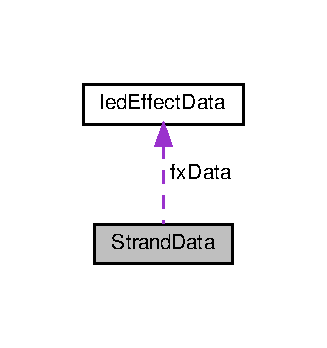
\includegraphics[width=157pt]{structStrandData__coll__graph}
\end{center}
\end{figure}
\subsection*{Public Attributes}
\begin{DoxyCompactItemize}
\item 
\mbox{\Hypertarget{structStrandData_a763350bc4cbb1f47fc30dae41862cc6e}\label{structStrandData_a763350bc4cbb1f47fc30dae41862cc6e}} 
led\+Type\+\_\+t {\bfseries led\+Type}
\item 
\hyperlink{vl53l0x__types_8h_aba7bc1797add20fe3efdf37ced1182c5}{uint8\+\_\+t} \hyperlink{structStrandData_a37a37b2a2d7eddbfc9c2ac8f448beddf}{strand\+Index}
\item 
\hyperlink{vl53l0x__types_8h_aba7bc1797add20fe3efdf37ced1182c5}{uint8\+\_\+t} \hyperlink{structStrandData_aff0894a9f07ac931f5242bc849b02a33}{update\+Leds}
\item 
\hyperlink{vl53l0x__types_8h_aba7bc1797add20fe3efdf37ced1182c5}{uint8\+\_\+t} \hyperlink{structStrandData_a627df352791351af4c92b6249608c58f}{bytes\+\_\+per\+\_\+pixel}
\item 
\hyperlink{vl53l0x__types_8h_a273cf69d639a59973b6019625df33e30}{uint16\+\_\+t} \hyperlink{structStrandData_af1b7eef4daa1ac9bbf830feed9bb8b46}{num\+Leds}
\item 
\hyperlink{vl53l0x__types_8h_a273cf69d639a59973b6019625df33e30}{uint16\+\_\+t} \hyperlink{structStrandData_aab77bb0d9f8a632662647c3aab7cf851}{strand\+Mem\+Length}
\item 
\hyperlink{vl53l0x__types_8h_a435d1572bf3f880d55459d9805097f62}{uint32\+\_\+t} $\ast$ \hyperlink{structStrandData_a187202b5a99913d82d24b81027bb007e}{strand\+Mem}
\item 
\hyperlink{vl53l0x__types_8h_a435d1572bf3f880d55459d9805097f62}{uint32\+\_\+t} \hyperlink{structStrandData_a8c39b96e1d498cfede3c5880f5b353b1}{strand\+Frame\+Length}
\item 
\mbox{\Hypertarget{structStrandData_a3e8674c134670e68889028982779627b}\label{structStrandData_a3e8674c134670e68889028982779627b}} 
\hyperlink{vl53l0x__types_8h_a435d1572bf3f880d55459d9805097f62}{uint32\+\_\+t} $\ast$ {\bfseries strand\+Frame\+Start}
\item 
\mbox{\Hypertarget{structStrandData_a039bb82617a17210019548381d18ff9c}\label{structStrandData_a039bb82617a17210019548381d18ff9c}} 
bool {\bfseries use\+\_\+dma}
\item 
\mbox{\Hypertarget{structStrandData_a1078b8e3e395bf7b79ce7d89659a3020}\label{structStrandData_a1078b8e3e395bf7b79ce7d89659a3020}} 
\hyperlink{structledEffectData}{led\+Effect\+Data\+\_\+t} $\ast$ {\bfseries fx\+Data}
\item 
Semaphore\+Handle\+\_\+t \hyperlink{structStrandData_aedec356f21caa5f3c3ec6c3615f90aff}{mem\+Semphr}
\item 
\hyperlink{vl53l0x__types_8h_aba7bc1797add20fe3efdf37ced1182c5}{uint8\+\_\+t} \hyperlink{structStrandData_ab6b3cfdc586b5a40497eb3d2931af76e}{spi\+\_\+channel\+\_\+no}
\item 
Timer\+Handle\+\_\+t \hyperlink{structStrandData_a68042468cd5f01417cb5f971feab4293}{refresh\+Timer}
\item 
rmt\+\_\+channel\+\_\+t \hyperlink{structStrandData_a50460c636123d0913362d3eab09f4b3f}{data\+Channel}
\item 
spi\+\_\+device\+\_\+handle\+\_\+t \hyperlink{structStrandData_aea9c3c5f3d3678e92723c7d2264b4f9e}{led\+S\+P\+I\+Handle}
\item 
Task\+Handle\+\_\+t \hyperlink{structStrandData_a0fbcfc7622e746b01484b7b943ffa913}{task\+\_\+handle}
\end{DoxyCompactItemize}


\subsection{Member Data Documentation}
\mbox{\Hypertarget{structStrandData_a627df352791351af4c92b6249608c58f}\label{structStrandData_a627df352791351af4c92b6249608c58f}} 
\index{Strand\+Data@{Strand\+Data}!bytes\+\_\+per\+\_\+pixel@{bytes\+\_\+per\+\_\+pixel}}
\index{bytes\+\_\+per\+\_\+pixel@{bytes\+\_\+per\+\_\+pixel}!Strand\+Data@{Strand\+Data}}
\subsubsection{\texorpdfstring{bytes\+\_\+per\+\_\+pixel}{bytes\_per\_pixel}}
{\footnotesize\ttfamily \hyperlink{vl53l0x__types_8h_aba7bc1797add20fe3efdf37ced1182c5}{uint8\+\_\+t} Strand\+Data\+::bytes\+\_\+per\+\_\+pixel}

$<$ update flag -\/ led mem has changed \mbox{\Hypertarget{structStrandData_a50460c636123d0913362d3eab09f4b3f}\label{structStrandData_a50460c636123d0913362d3eab09f4b3f}} 
\index{Strand\+Data@{Strand\+Data}!data\+Channel@{data\+Channel}}
\index{data\+Channel@{data\+Channel}!Strand\+Data@{Strand\+Data}}
\subsubsection{\texorpdfstring{data\+Channel}{dataChannel}}
{\footnotesize\ttfamily rmt\+\_\+channel\+\_\+t Strand\+Data\+::data\+Channel}

$<$ handle for the effect refresh timer \mbox{\Hypertarget{structStrandData_aea9c3c5f3d3678e92723c7d2264b4f9e}\label{structStrandData_aea9c3c5f3d3678e92723c7d2264b4f9e}} 
\index{Strand\+Data@{Strand\+Data}!led\+S\+P\+I\+Handle@{led\+S\+P\+I\+Handle}}
\index{led\+S\+P\+I\+Handle@{led\+S\+P\+I\+Handle}!Strand\+Data@{Strand\+Data}}
\subsubsection{\texorpdfstring{led\+S\+P\+I\+Handle}{ledSPIHandle}}
{\footnotesize\ttfamily spi\+\_\+device\+\_\+handle\+\_\+t Strand\+Data\+::led\+S\+P\+I\+Handle}

$<$ T\+O\+DO\+: replace this \& next with union/bitfield \mbox{\Hypertarget{structStrandData_aedec356f21caa5f3c3ec6c3615f90aff}\label{structStrandData_aedec356f21caa5f3c3ec6c3615f90aff}} 
\index{Strand\+Data@{Strand\+Data}!mem\+Semphr@{mem\+Semphr}}
\index{mem\+Semphr@{mem\+Semphr}!Strand\+Data@{Strand\+Data}}
\subsubsection{\texorpdfstring{mem\+Semphr}{memSemphr}}
{\footnotesize\ttfamily Semaphore\+Handle\+\_\+t Strand\+Data\+::mem\+Semphr}

$<$ pointer to led effect data \mbox{\Hypertarget{structStrandData_af1b7eef4daa1ac9bbf830feed9bb8b46}\label{structStrandData_af1b7eef4daa1ac9bbf830feed9bb8b46}} 
\index{Strand\+Data@{Strand\+Data}!num\+Leds@{num\+Leds}}
\index{num\+Leds@{num\+Leds}!Strand\+Data@{Strand\+Data}}
\subsubsection{\texorpdfstring{num\+Leds}{numLeds}}
{\footnotesize\ttfamily \hyperlink{vl53l0x__types_8h_a273cf69d639a59973b6019625df33e30}{uint16\+\_\+t} Strand\+Data\+::num\+Leds}

$<$ bytes per pixel \mbox{\Hypertarget{structStrandData_a68042468cd5f01417cb5f971feab4293}\label{structStrandData_a68042468cd5f01417cb5f971feab4293}} 
\index{Strand\+Data@{Strand\+Data}!refresh\+Timer@{refresh\+Timer}}
\index{refresh\+Timer@{refresh\+Timer}!Strand\+Data@{Strand\+Data}}
\subsubsection{\texorpdfstring{refresh\+Timer}{refreshTimer}}
{\footnotesize\ttfamily Timer\+Handle\+\_\+t Strand\+Data\+::refresh\+Timer}

$<$ the channel of the S\+PI peripheral used \mbox{\Hypertarget{structStrandData_ab6b3cfdc586b5a40497eb3d2931af76e}\label{structStrandData_ab6b3cfdc586b5a40497eb3d2931af76e}} 
\index{Strand\+Data@{Strand\+Data}!spi\+\_\+channel\+\_\+no@{spi\+\_\+channel\+\_\+no}}
\index{spi\+\_\+channel\+\_\+no@{spi\+\_\+channel\+\_\+no}!Strand\+Data@{Strand\+Data}}
\subsubsection{\texorpdfstring{spi\+\_\+channel\+\_\+no}{spi\_channel\_no}}
{\footnotesize\ttfamily \hyperlink{vl53l0x__types_8h_aba7bc1797add20fe3efdf37ced1182c5}{uint8\+\_\+t} Strand\+Data\+::spi\+\_\+channel\+\_\+no}

$<$ sempahore for led data access \mbox{\Hypertarget{structStrandData_a8c39b96e1d498cfede3c5880f5b353b1}\label{structStrandData_a8c39b96e1d498cfede3c5880f5b353b1}} 
\index{Strand\+Data@{Strand\+Data}!strand\+Frame\+Length@{strand\+Frame\+Length}}
\index{strand\+Frame\+Length@{strand\+Frame\+Length}!Strand\+Data@{Strand\+Data}}
\subsubsection{\texorpdfstring{strand\+Frame\+Length}{strandFrameLength}}
{\footnotesize\ttfamily \hyperlink{vl53l0x__types_8h_a435d1572bf3f880d55459d9805097f62}{uint32\+\_\+t} Strand\+Data\+::strand\+Frame\+Length}

$<$ pointer to L\+ED data \mbox{\Hypertarget{structStrandData_a37a37b2a2d7eddbfc9c2ac8f448beddf}\label{structStrandData_a37a37b2a2d7eddbfc9c2ac8f448beddf}} 
\index{Strand\+Data@{Strand\+Data}!strand\+Index@{strand\+Index}}
\index{strand\+Index@{strand\+Index}!Strand\+Data@{Strand\+Data}}
\subsubsection{\texorpdfstring{strand\+Index}{strandIndex}}
{\footnotesize\ttfamily \hyperlink{vl53l0x__types_8h_aba7bc1797add20fe3efdf37ced1182c5}{uint8\+\_\+t} Strand\+Data\+::strand\+Index}

$<$ type of L\+ED \mbox{\Hypertarget{structStrandData_a187202b5a99913d82d24b81027bb007e}\label{structStrandData_a187202b5a99913d82d24b81027bb007e}} 
\index{Strand\+Data@{Strand\+Data}!strand\+Mem@{strand\+Mem}}
\index{strand\+Mem@{strand\+Mem}!Strand\+Data@{Strand\+Data}}
\subsubsection{\texorpdfstring{strand\+Mem}{strandMem}}
{\footnotesize\ttfamily \hyperlink{vl53l0x__types_8h_a435d1572bf3f880d55459d9805097f62}{uint32\+\_\+t}$\ast$ Strand\+Data\+::strand\+Mem}

$<$ length of memory \mbox{\Hypertarget{structStrandData_aab77bb0d9f8a632662647c3aab7cf851}\label{structStrandData_aab77bb0d9f8a632662647c3aab7cf851}} 
\index{Strand\+Data@{Strand\+Data}!strand\+Mem\+Length@{strand\+Mem\+Length}}
\index{strand\+Mem\+Length@{strand\+Mem\+Length}!Strand\+Data@{Strand\+Data}}
\subsubsection{\texorpdfstring{strand\+Mem\+Length}{strandMemLength}}
{\footnotesize\ttfamily \hyperlink{vl53l0x__types_8h_a273cf69d639a59973b6019625df33e30}{uint16\+\_\+t} Strand\+Data\+::strand\+Mem\+Length}

$<$ num leds in strand \mbox{\Hypertarget{structStrandData_a0fbcfc7622e746b01484b7b943ffa913}\label{structStrandData_a0fbcfc7622e746b01484b7b943ffa913}} 
\index{Strand\+Data@{Strand\+Data}!task\+\_\+handle@{task\+\_\+handle}}
\index{task\+\_\+handle@{task\+\_\+handle}!Strand\+Data@{Strand\+Data}}
\subsubsection{\texorpdfstring{task\+\_\+handle}{task\_handle}}
{\footnotesize\ttfamily Task\+Handle\+\_\+t Strand\+Data\+::task\+\_\+handle}

$<$ spi device handle \mbox{\Hypertarget{structStrandData_aff0894a9f07ac931f5242bc849b02a33}\label{structStrandData_aff0894a9f07ac931f5242bc849b02a33}} 
\index{Strand\+Data@{Strand\+Data}!update\+Leds@{update\+Leds}}
\index{update\+Leds@{update\+Leds}!Strand\+Data@{Strand\+Data}}
\subsubsection{\texorpdfstring{update\+Leds}{updateLeds}}
{\footnotesize\ttfamily \hyperlink{vl53l0x__types_8h_aba7bc1797add20fe3efdf37ced1182c5}{uint8\+\_\+t} Strand\+Data\+::update\+Leds}

$<$ index of the current strand 

The documentation for this struct was generated from the following file\+:\begin{DoxyCompactItemize}
\item 
Utils/Led\+Effects.\+h\end{DoxyCompactItemize}

\hypertarget{structstruct}{}\section{struct Struct Reference}
\label{structstruct}\index{struct@{struct}}


{\ttfamily \#include $<$M\+F\+R\+C522\+\_\+\+Driver.\+h$>$}



Collaboration diagram for struct\+:\nopagebreak
\begin{figure}[H]
\begin{center}
\leavevmode
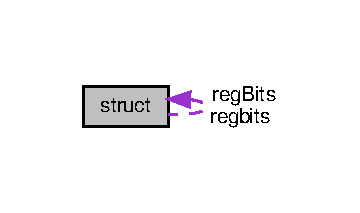
\includegraphics[width=173pt]{structstruct__coll__graph}
\end{center}
\end{figure}
\subsection*{Public Attributes}
\begin{DoxyCompactItemize}
\item 
\hyperlink{vl53l0x__types_8h_aba7bc1797add20fe3efdf37ced1182c5}{uint8\+\_\+t} \hyperlink{structstruct_a98137858bbe84718f27b15f7f524ee23}{reserved\+\_\+0}
\item 
\begin{tabbing}
xx\=xx\=xx\=xx\=xx\=xx\=xx\=xx\=xx\=\kill
union \{\\
\>\hyperlink{vl53l0x__types_8h_aba7bc1797add20fe3efdf37ced1182c5}{uint8\_t} {\bfseries regval}\\
\>struct \{\\
\>\>\hyperlink{vl53l0x__types_8h_aba7bc1797add20fe3efdf37ced1182c5}{uint8\_t} {\bfseries command}: 4\\
\>\>\hyperlink{vl53l0x__types_8h_aba7bc1797add20fe3efdf37ced1182c5}{uint8\_t} {\bfseries pwr\_down}: 1\\
\>\>\hyperlink{vl53l0x__types_8h_aba7bc1797add20fe3efdf37ced1182c5}{uint8\_t} {\bfseries rcv\_off}: 1\\
\>\>\hyperlink{vl53l0x__types_8h_aba7bc1797add20fe3efdf37ced1182c5}{uint8\_t} {\bfseries rsvd\_0}: 2\\
\>\} {\bfseries regbits}\\
\} \hyperlink{structstruct_a4ad4bf4bdf213b87b9b52e993c0a7793}{command\_reg}\\

\end{tabbing}\item 
\begin{tabbing}
xx\=xx\=xx\=xx\=xx\=xx\=xx\=xx\=xx\=\kill
union \{\\
\>\hyperlink{vl53l0x__types_8h_aba7bc1797add20fe3efdf37ced1182c5}{uint8\_t} {\bfseries regval}\\
\>struct \{\\
\>\>\hyperlink{vl53l0x__types_8h_aba7bc1797add20fe3efdf37ced1182c5}{uint8\_t} {\bfseries tmr\_irq\_en}: 1\\
\>\>\hyperlink{vl53l0x__types_8h_aba7bc1797add20fe3efdf37ced1182c5}{uint8\_t} {\bfseries err\_irq\_en}: 1\\
\>\>\hyperlink{vl53l0x__types_8h_aba7bc1797add20fe3efdf37ced1182c5}{uint8\_t} {\bfseries flo\_irq\_en}: 1\\
\>\>\hyperlink{vl53l0x__types_8h_aba7bc1797add20fe3efdf37ced1182c5}{uint8\_t} {\bfseries fhi\_irq\_en}: 1\\
\>\>\hyperlink{vl53l0x__types_8h_aba7bc1797add20fe3efdf37ced1182c5}{uint8\_t} {\bfseries idle\_irq\_en}: 1\\
\>\>\hyperlink{vl53l0x__types_8h_aba7bc1797add20fe3efdf37ced1182c5}{uint8\_t} {\bfseries rx\_irq\_en}: 1\\
\>\>\hyperlink{vl53l0x__types_8h_aba7bc1797add20fe3efdf37ced1182c5}{uint8\_t} {\bfseries tx\_irq\_en}: 1\\
\>\>\hyperlink{vl53l0x__types_8h_aba7bc1797add20fe3efdf37ced1182c5}{uint8\_t} {\bfseries irq\_invert}: 1\\
\>\} {\bfseries regbits}\\
\} \hyperlink{structstruct_aaaae33aa946f3e8116c2c852830d8291}{command\_en\_reg}\\

\end{tabbing}\item 
\begin{tabbing}
xx\=xx\=xx\=xx\=xx\=xx\=xx\=xx\=xx\=\kill
union \{\\
\>\hyperlink{vl53l0x__types_8h_aba7bc1797add20fe3efdf37ced1182c5}{uint8\_t} {\bfseries regval}\\
\>struct \{\\
\>\>\hyperlink{vl53l0x__types_8h_aba7bc1797add20fe3efdf37ced1182c5}{uint8\_t} {\bfseries rsvd\_0}: 2\\
\>\>\hyperlink{vl53l0x__types_8h_aba7bc1797add20fe3efdf37ced1182c5}{uint8\_t} {\bfseries crc\_irq\_en}: 1\\
\>\>\hyperlink{vl53l0x__types_8h_aba7bc1797add20fe3efdf37ced1182c5}{uint8\_t} {\bfseries rsvd\_1}: 1\\
\>\>\hyperlink{vl53l0x__types_8h_aba7bc1797add20fe3efdf37ced1182c5}{uint8\_t} {\bfseries mfin\_irq\_en}: 1\\
\>\>\hyperlink{vl53l0x__types_8h_aba7bc1797add20fe3efdf37ced1182c5}{uint8\_t} {\bfseries rsvd\_2}: 2\\
\>\>\hyperlink{vl53l0x__types_8h_aba7bc1797add20fe3efdf37ced1182c5}{uint8\_t} {\bfseries irq\_pp\_od}: 1\\
\>\} {\bfseries regbits}\\
\} \hyperlink{structstruct_aa5145a6200deee0b11aa3f5f5cc259f8}{irq\_passing\_reg}\\

\end{tabbing}\item 
\begin{tabbing}
xx\=xx\=xx\=xx\=xx\=xx\=xx\=xx\=xx\=\kill
union \{\\
\>\hyperlink{vl53l0x__types_8h_aba7bc1797add20fe3efdf37ced1182c5}{uint8\_t} {\bfseries regval}\\
\>struct \{\\
\>\>\hyperlink{vl53l0x__types_8h_aba7bc1797add20fe3efdf37ced1182c5}{uint8\_t} {\bfseries tmr\_irq}: 1\\
\>\>\hyperlink{vl53l0x__types_8h_aba7bc1797add20fe3efdf37ced1182c5}{uint8\_t} {\bfseries err\_irq}: 1\\
\>\>\hyperlink{vl53l0x__types_8h_aba7bc1797add20fe3efdf37ced1182c5}{uint8\_t} {\bfseries flo\_irq}: 1\\
\>\>\hyperlink{vl53l0x__types_8h_aba7bc1797add20fe3efdf37ced1182c5}{uint8\_t} {\bfseries fli\_irq}: 1\\
\>\>\hyperlink{vl53l0x__types_8h_aba7bc1797add20fe3efdf37ced1182c5}{uint8\_t} {\bfseries idle\_irq}: 1\\
\>\>\hyperlink{vl53l0x__types_8h_aba7bc1797add20fe3efdf37ced1182c5}{uint8\_t} {\bfseries rx\_irq}: 1\\
\>\>\hyperlink{vl53l0x__types_8h_aba7bc1797add20fe3efdf37ced1182c5}{uint8\_t} {\bfseries tx\_irq}: 1\\
\>\>\hyperlink{vl53l0x__types_8h_aba7bc1797add20fe3efdf37ced1182c5}{uint8\_t} {\bfseries irq\_set}: 1\\
\>\} {\bfseries regbits}\\
\} \hyperlink{structstruct_a2732e86723cc2f90559edb4721ccb79a}{com\_irq\_reg}\\

\end{tabbing}\item 
\begin{tabbing}
xx\=xx\=xx\=xx\=xx\=xx\=xx\=xx\=xx\=\kill
union \{\\
\>\hyperlink{vl53l0x__types_8h_aba7bc1797add20fe3efdf37ced1182c5}{uint8\_t} {\bfseries regByte}\\
\>struct \{\\
\>\>\hyperlink{vl53l0x__types_8h_aba7bc1797add20fe3efdf37ced1182c5}{uint8\_t} {\bfseries rsvd\_0}: 2\\
\>\>\hyperlink{vl53l0x__types_8h_aba7bc1797add20fe3efdf37ced1182c5}{uint8\_t} {\bfseries crc\_irq}: 1\\
\>\>\hyperlink{vl53l0x__types_8h_aba7bc1797add20fe3efdf37ced1182c5}{uint8\_t} {\bfseries rsvd\_1}: 1\\
\>\>\hyperlink{vl53l0x__types_8h_aba7bc1797add20fe3efdf37ced1182c5}{uint8\_t} {\bfseries mfin\_irq}: 1\\
\>\>\hyperlink{vl53l0x__types_8h_aba7bc1797add20fe3efdf37ced1182c5}{uint8\_t} {\bfseries rsvd\_2}: 2\\
\>\>\hyperlink{vl53l0x__types_8h_aba7bc1797add20fe3efdf37ced1182c5}{uint8\_t} {\bfseries irq\_set\_2}: 1\\
\>\} {\bfseries regBits}\\
\} \hyperlink{structstruct_afe48e85a7251b6182a5f8a6be7344d5f}{div\_irq\_reg}\\

\end{tabbing}\item 
\begin{tabbing}
xx\=xx\=xx\=xx\=xx\=xx\=xx\=xx\=xx\=\kill
union \{\\
\>\hyperlink{vl53l0x__types_8h_aba7bc1797add20fe3efdf37ced1182c5}{uint8\_t} {\bfseries regByte}\\
\>struct \{\\
\>\>\hyperlink{vl53l0x__types_8h_aba7bc1797add20fe3efdf37ced1182c5}{uint8\_t} {\bfseries protocol\_err}: 1\\
\>\>\hyperlink{vl53l0x__types_8h_aba7bc1797add20fe3efdf37ced1182c5}{uint8\_t} {\bfseries parity\_err}: 1\\
\>\>\hyperlink{vl53l0x__types_8h_aba7bc1797add20fe3efdf37ced1182c5}{uint8\_t} {\bfseries crc\_err}: 1\\
\>\>\hyperlink{vl53l0x__types_8h_aba7bc1797add20fe3efdf37ced1182c5}{uint8\_t} {\bfseries coll\_err}: 1\\
\>\>\hyperlink{vl53l0x__types_8h_aba7bc1797add20fe3efdf37ced1182c5}{uint8\_t} {\bfseries buffer\_ovr\_err}: 1\\
\>\>\hyperlink{vl53l0x__types_8h_aba7bc1797add20fe3efdf37ced1182c5}{uint8\_t} {\bfseries rsvd\_0}: 1\\
\>\>\hyperlink{vl53l0x__types_8h_aba7bc1797add20fe3efdf37ced1182c5}{uint8\_t} {\bfseries tempr\_err}: 1\\
\>\>\hyperlink{vl53l0x__types_8h_aba7bc1797add20fe3efdf37ced1182c5}{uint8\_t} {\bfseries wrt\_err}: 1\\
\>\} {\bfseries regBits}\\
\} \hyperlink{structstruct_a712e569a0385acfa82147baac2dd096b}{error\_reg}\\

\end{tabbing}\item 
\begin{tabbing}
xx\=xx\=xx\=xx\=xx\=xx\=xx\=xx\=xx\=\kill
union \{\\
\>\hyperlink{vl53l0x__types_8h_aba7bc1797add20fe3efdf37ced1182c5}{uint8\_t} {\bfseries regByte}\\
\>struct \{\\
\>\>\hyperlink{vl53l0x__types_8h_aba7bc1797add20fe3efdf37ced1182c5}{uint8\_t} {\bfseries fifo\_lo\_alert}: 1\\
\>\>\hyperlink{vl53l0x__types_8h_aba7bc1797add20fe3efdf37ced1182c5}{uint8\_t} {\bfseries fifo\_hi\_alert}: 1\\
\>\>\hyperlink{vl53l0x__types_8h_aba7bc1797add20fe3efdf37ced1182c5}{uint8\_t} {\bfseries rsvd\_0}: 1\\
\>\>\hyperlink{vl53l0x__types_8h_aba7bc1797add20fe3efdf37ced1182c5}{uint8\_t} {\bfseries tmr\_running}: 1\\
\>\>\hyperlink{vl53l0x__types_8h_aba7bc1797add20fe3efdf37ced1182c5}{uint8\_t} {\bfseries irq\_alert}: 1\\
\>\>\hyperlink{vl53l0x__types_8h_aba7bc1797add20fe3efdf37ced1182c5}{uint8\_t} {\bfseries crc\_ready}: 1\\
\>\>\hyperlink{vl53l0x__types_8h_aba7bc1797add20fe3efdf37ced1182c5}{uint8\_t} {\bfseries crc\_ok}: 1\\
\>\>\hyperlink{vl53l0x__types_8h_aba7bc1797add20fe3efdf37ced1182c5}{uint8\_t} {\bfseries rsvd\_1}: 1\\
\>\} {\bfseries regBits}\\
\} \hyperlink{structstruct_a3af413aba8342123dc8bd7d2d5e6663c}{status\_1\_reg}\\

\end{tabbing}\item 
\begin{tabbing}
xx\=xx\=xx\=xx\=xx\=xx\=xx\=xx\=xx\=\kill
union \{\\
\>\hyperlink{vl53l0x__types_8h_aba7bc1797add20fe3efdf37ced1182c5}{uint8\_t} {\bfseries regByte}\\
\>struct \{\\
\>\>\hyperlink{vl53l0x__types_8h_aba7bc1797add20fe3efdf37ced1182c5}{uint8\_t} {\bfseries modem\_state}: 2\\
\>\>\hyperlink{vl53l0x__types_8h_aba7bc1797add20fe3efdf37ced1182c5}{uint8\_t} {\bfseries mifare\_crypt1\_on}: 2\\
\>\>\hyperlink{vl53l0x__types_8h_aba7bc1797add20fe3efdf37ced1182c5}{uint8\_t} {\bfseries rsvd\_0}: 2\\
\>\>\hyperlink{vl53l0x__types_8h_aba7bc1797add20fe3efdf37ced1182c5}{uint8\_t} {\bfseries i2c\_force\_hs}: 1\\
\>\>\hyperlink{vl53l0x__types_8h_aba7bc1797add20fe3efdf37ced1182c5}{uint8\_t} {\bfseries temp\_sens\_clr}: 1\\
\>\} {\bfseries regBits}\\
\} \hyperlink{structstruct_a01781aef0edd49d172a2b5df5ec1c138}{status\_2\_reg}\\

\end{tabbing}\item 
\begin{tabbing}
xx\=xx\=xx\=xx\=xx\=xx\=xx\=xx\=xx\=\kill
union \{\\
\>\hyperlink{vl53l0x__types_8h_aba7bc1797add20fe3efdf37ced1182c5}{uint8\_t} {\bfseries regByte}\\
\>struct \{\\
\>\>\hyperlink{vl53l0x__types_8h_aba7bc1797add20fe3efdf37ced1182c5}{uint8\_t} {\bfseries fifo\_data}: 8\\
\>\} {\bfseries regBits}\\
\} \hyperlink{structstruct_a0c4836d627c24316e95a54b24bc569a9}{fifo\_data\_reg}\\

\end{tabbing}\item 
\begin{tabbing}
xx\=xx\=xx\=xx\=xx\=xx\=xx\=xx\=xx\=\kill
union \{\\
\>\hyperlink{vl53l0x__types_8h_aba7bc1797add20fe3efdf37ced1182c5}{uint8\_t} {\bfseries regByte}\\
\>struct \{\\
\>\>\hyperlink{vl53l0x__types_8h_aba7bc1797add20fe3efdf37ced1182c5}{uint8\_t} {\bfseries fifo\_level}: 7\\
\>\>\hyperlink{vl53l0x__types_8h_aba7bc1797add20fe3efdf37ced1182c5}{uint8\_t} {\bfseries flush\_buffer}: 1\\
\>\} {\bfseries regBits}\\
\} \hyperlink{structstruct_a8d30208f95a8160e46c989f5bcb6d770}{fifo\_lvl\_reg}\\

\end{tabbing}\item 
\begin{tabbing}
xx\=xx\=xx\=xx\=xx\=xx\=xx\=xx\=xx\=\kill
union \{\\
\>\hyperlink{vl53l0x__types_8h_aba7bc1797add20fe3efdf37ced1182c5}{uint8\_t} {\bfseries regByte}\\
\>struct \{\\
\>\>\hyperlink{vl53l0x__types_8h_aba7bc1797add20fe3efdf37ced1182c5}{uint8\_t} {\bfseries fifo\_watermark}: 6\\
\>\>\hyperlink{vl53l0x__types_8h_aba7bc1797add20fe3efdf37ced1182c5}{uint8\_t} {\bfseries rsvd\_0}: 2\\
\>\} {\bfseries regBits}\\
\} \hyperlink{structstruct_a9d47568f82f8554a6869d7e026ff9382}{fifo\_watermark\_reg}\\

\end{tabbing}\item 
\begin{tabbing}
xx\=xx\=xx\=xx\=xx\=xx\=xx\=xx\=xx\=\kill
union \{\\
\>\hyperlink{vl53l0x__types_8h_aba7bc1797add20fe3efdf37ced1182c5}{uint8\_t} {\bfseries regByte}\\
\>struct \{\\
\>\>\hyperlink{vl53l0x__types_8h_aba7bc1797add20fe3efdf37ced1182c5}{uint8\_t} {\bfseries rx\_last\_bits}: 3\\
\>\>\hyperlink{vl53l0x__types_8h_aba7bc1797add20fe3efdf37ced1182c5}{uint8\_t} {\bfseries rsvd\_0}: 3\\
\>\>\hyperlink{vl53l0x__types_8h_aba7bc1797add20fe3efdf37ced1182c5}{uint8\_t} {\bfseries tmr\_start\_now}: 1\\
\>\>\hyperlink{vl53l0x__types_8h_aba7bc1797add20fe3efdf37ced1182c5}{uint8\_t} {\bfseries tmr\_stop\_now}: 1\\
\>\} {\bfseries regBits}\\
\} \hyperlink{structstruct_a721f276d7231c2e85a8fd2c78e554de4}{control\_reg}\\

\end{tabbing}\item 
\begin{tabbing}
xx\=xx\=xx\=xx\=xx\=xx\=xx\=xx\=xx\=\kill
union \{\\
\>\hyperlink{vl53l0x__types_8h_aba7bc1797add20fe3efdf37ced1182c5}{uint8\_t} {\bfseries regByte}\\
\>struct \{\\
\>\>\hyperlink{vl53l0x__types_8h_aba7bc1797add20fe3efdf37ced1182c5}{uint8\_t} {\bfseries tx\_last\_bits}: 3\\
\>\>\hyperlink{vl53l0x__types_8h_aba7bc1797add20fe3efdf37ced1182c5}{uint8\_t} {\bfseries rsvd\_0}: 1\\
\>\>\hyperlink{vl53l0x__types_8h_aba7bc1797add20fe3efdf37ced1182c5}{uint8\_t} {\bfseries rx\_align}: 3\\
\>\>\hyperlink{vl53l0x__types_8h_aba7bc1797add20fe3efdf37ced1182c5}{uint8\_t} {\bfseries start\_send}: 1\\
\>\} {\bfseries regBits}\\
\} \hyperlink{structstruct_a875453616cf061da36e0ed90d46d380c}{bitframe\_reg}\\

\end{tabbing}\item 
\begin{tabbing}
xx\=xx\=xx\=xx\=xx\=xx\=xx\=xx\=xx\=\kill
union \{\\
\>\hyperlink{vl53l0x__types_8h_aba7bc1797add20fe3efdf37ced1182c5}{uint8\_t} {\bfseries regByte}\\
\>struct \{\\
\>\>\hyperlink{vl53l0x__types_8h_aba7bc1797add20fe3efdf37ced1182c5}{uint8\_t} {\bfseries collision\_pos}: 5\\
\>\>\hyperlink{vl53l0x__types_8h_aba7bc1797add20fe3efdf37ced1182c5}{uint8\_t} {\bfseries coll\_pos\_invalid}: 1\\
\>\>\hyperlink{vl53l0x__types_8h_aba7bc1797add20fe3efdf37ced1182c5}{uint8\_t} {\bfseries rsvd\_0}: 1\\
\>\>\hyperlink{vl53l0x__types_8h_aba7bc1797add20fe3efdf37ced1182c5}{uint8\_t} {\bfseries clr\_rx\_on\_collision}: 1\\
\>\} {\bfseries regBits}\\
\} \hyperlink{structstruct_ac0256f75f90f8e0587b10bd273eb127e}{collision\_reg}\\

\end{tabbing}\item 
\hyperlink{vl53l0x__types_8h_aba7bc1797add20fe3efdf37ced1182c5}{uint8\+\_\+t} \hyperlink{structstruct_a2024e673a4ec7a81da3a35fe74ff6a51}{reserved\+\_\+1}
\item 
\hyperlink{vl53l0x__types_8h_aba7bc1797add20fe3efdf37ced1182c5}{uint8\+\_\+t} \hyperlink{structstruct_a7be82c5d2760e33db4ce747304d98ffe}{reserved\+\_\+2}
\item 
\begin{tabbing}
xx\=xx\=xx\=xx\=xx\=xx\=xx\=xx\=xx\=\kill
union \{\\
\>\hyperlink{vl53l0x__types_8h_aba7bc1797add20fe3efdf37ced1182c5}{uint8\_t} {\bfseries regByte}\\
\>struct \{\\
\>\>\hyperlink{vl53l0x__types_8h_aba7bc1797add20fe3efdf37ced1182c5}{uint8\_t} {\bfseries crc\_preset}: 2\\
\>\>\hyperlink{vl53l0x__types_8h_aba7bc1797add20fe3efdf37ced1182c5}{uint8\_t} {\bfseries rsvd\_0}: 1\\
\>\>\hyperlink{vl53l0x__types_8h_aba7bc1797add20fe3efdf37ced1182c5}{uint8\_t} {\bfseries pol\_mf\_in}: 1\\
\>\>\hyperlink{vl53l0x__types_8h_aba7bc1797add20fe3efdf37ced1182c5}{uint8\_t} {\bfseries rsvd\_1}: 1\\
\>\>\hyperlink{vl53l0x__types_8h_aba7bc1797add20fe3efdf37ced1182c5}{uint8\_t} {\bfseries tx\_wait\_rf}: 1\\
\>\>\hyperlink{vl53l0x__types_8h_aba7bc1797add20fe3efdf37ced1182c5}{uint8\_t} {\bfseries rsvd\_2}: 1\\
\>\>\hyperlink{vl53l0x__types_8h_aba7bc1797add20fe3efdf37ced1182c5}{uint8\_t} {\bfseries crc\_msb\_first}: 1\\
\>\} {\bfseries regBits}\\
\} \hyperlink{structstruct_ad6f64ca923a5a6d1ed05aae900c7889d}{mode\_register}\\

\end{tabbing}\item 
\begin{tabbing}
xx\=xx\=xx\=xx\=xx\=xx\=xx\=xx\=xx\=\kill
union \{\\
\>\hyperlink{vl53l0x__types_8h_aba7bc1797add20fe3efdf37ced1182c5}{uint8\_t} {\bfseries regByte}\\
\>struct \{\\
\>\>\hyperlink{vl53l0x__types_8h_aba7bc1797add20fe3efdf37ced1182c5}{uint8\_t} {\bfseries rsvd\_0}: 3\\
\>\>\hyperlink{vl53l0x__types_8h_aba7bc1797add20fe3efdf37ced1182c5}{uint8\_t} {\bfseries invert\_modulation}: 1\\
\>\>\hyperlink{vl53l0x__types_8h_aba7bc1797add20fe3efdf37ced1182c5}{uint8\_t} {\bfseries tx\_speed}: 3\\
\>\>\hyperlink{vl53l0x__types_8h_aba7bc1797add20fe3efdf37ced1182c5}{uint8\_t} {\bfseries tx\_crc\_en}: 1\\
\>\} {\bfseries regBits}\\
\} \hyperlink{structstruct_a1dd825787c2f3275c00463af6fb446a8}{tx\_mode\_reg}\\

\end{tabbing}\item 
\begin{tabbing}
xx\=xx\=xx\=xx\=xx\=xx\=xx\=xx\=xx\=\kill
union \{\\
\>\hyperlink{vl53l0x__types_8h_aba7bc1797add20fe3efdf37ced1182c5}{uint8\_t} {\bfseries regByte}\\
\>struct \{\\
\>\>\hyperlink{vl53l0x__types_8h_aba7bc1797add20fe3efdf37ced1182c5}{uint8\_t} {\bfseries rsvd\_0}: 2\\
\>\>\hyperlink{vl53l0x__types_8h_aba7bc1797add20fe3efdf37ced1182c5}{uint8\_t} {\bfseries rx\_multiple}: 1\\
\>\>\hyperlink{vl53l0x__types_8h_aba7bc1797add20fe3efdf37ced1182c5}{uint8\_t} {\bfseries rx\_no\_err}: 1\\
\>\>\hyperlink{vl53l0x__types_8h_aba7bc1797add20fe3efdf37ced1182c5}{uint8\_t} {\bfseries rx\_speed}: 3\\
\>\>\hyperlink{vl53l0x__types_8h_aba7bc1797add20fe3efdf37ced1182c5}{uint8\_t} {\bfseries rx\_crc\_en}: 1\\
\>\} {\bfseries regBits}\\
\} \hyperlink{structstruct_a7209689ecea0fda4ba3ccddf5234e452}{rx\_mode\_reg}\\

\end{tabbing}\end{DoxyCompactItemize}


\subsection{Detailed Description}
Gonna give this struct register thing a go, might be easier to manager device settings? 

\subsection{Member Data Documentation}
\mbox{\Hypertarget{structstruct_a875453616cf061da36e0ed90d46d380c}\label{structstruct_a875453616cf061da36e0ed90d46d380c}} 
\index{struct@{struct}!bitframe\+\_\+reg@{bitframe\+\_\+reg}}
\index{bitframe\+\_\+reg@{bitframe\+\_\+reg}!struct@{struct}}
\subsubsection{\texorpdfstring{bitframe\+\_\+reg}{bitframe\_reg}}
{\footnotesize\ttfamily union \{ ... \}   struct\+::bitframe\+\_\+reg}

0x0D \mbox{\Hypertarget{structstruct_ac0256f75f90f8e0587b10bd273eb127e}\label{structstruct_ac0256f75f90f8e0587b10bd273eb127e}} 
\index{struct@{struct}!collision\+\_\+reg@{collision\+\_\+reg}}
\index{collision\+\_\+reg@{collision\+\_\+reg}!struct@{struct}}
\subsubsection{\texorpdfstring{collision\+\_\+reg}{collision\_reg}}
{\footnotesize\ttfamily union \{ ... \}   struct\+::collision\+\_\+reg}

0x0E \mbox{\Hypertarget{structstruct_a2732e86723cc2f90559edb4721ccb79a}\label{structstruct_a2732e86723cc2f90559edb4721ccb79a}} 
\index{struct@{struct}!com\+\_\+irq\+\_\+reg@{com\+\_\+irq\+\_\+reg}}
\index{com\+\_\+irq\+\_\+reg@{com\+\_\+irq\+\_\+reg}!struct@{struct}}
\subsubsection{\texorpdfstring{com\+\_\+irq\+\_\+reg}{com\_irq\_reg}}
{\footnotesize\ttfamily union \{ ... \}   struct\+::com\+\_\+irq\+\_\+reg}

0x04 \mbox{\Hypertarget{structstruct_aaaae33aa946f3e8116c2c852830d8291}\label{structstruct_aaaae33aa946f3e8116c2c852830d8291}} 
\index{struct@{struct}!command\+\_\+en\+\_\+reg@{command\+\_\+en\+\_\+reg}}
\index{command\+\_\+en\+\_\+reg@{command\+\_\+en\+\_\+reg}!struct@{struct}}
\subsubsection{\texorpdfstring{command\+\_\+en\+\_\+reg}{command\_en\_reg}}
{\footnotesize\ttfamily union \{ ... \}   struct\+::command\+\_\+en\+\_\+reg}

0x02 \mbox{\Hypertarget{structstruct_a4ad4bf4bdf213b87b9b52e993c0a7793}\label{structstruct_a4ad4bf4bdf213b87b9b52e993c0a7793}} 
\index{struct@{struct}!command\+\_\+reg@{command\+\_\+reg}}
\index{command\+\_\+reg@{command\+\_\+reg}!struct@{struct}}
\subsubsection{\texorpdfstring{command\+\_\+reg}{command\_reg}}
{\footnotesize\ttfamily union \{ ... \}   struct\+::command\+\_\+reg}

0x01 \mbox{\Hypertarget{structstruct_a721f276d7231c2e85a8fd2c78e554de4}\label{structstruct_a721f276d7231c2e85a8fd2c78e554de4}} 
\index{struct@{struct}!control\+\_\+reg@{control\+\_\+reg}}
\index{control\+\_\+reg@{control\+\_\+reg}!struct@{struct}}
\subsubsection{\texorpdfstring{control\+\_\+reg}{control\_reg}}
{\footnotesize\ttfamily union \{ ... \}   struct\+::control\+\_\+reg}

0x0C \mbox{\Hypertarget{structstruct_afe48e85a7251b6182a5f8a6be7344d5f}\label{structstruct_afe48e85a7251b6182a5f8a6be7344d5f}} 
\index{struct@{struct}!div\+\_\+irq\+\_\+reg@{div\+\_\+irq\+\_\+reg}}
\index{div\+\_\+irq\+\_\+reg@{div\+\_\+irq\+\_\+reg}!struct@{struct}}
\subsubsection{\texorpdfstring{div\+\_\+irq\+\_\+reg}{div\_irq\_reg}}
{\footnotesize\ttfamily union \{ ... \}   struct\+::div\+\_\+irq\+\_\+reg}

0x05 \mbox{\Hypertarget{structstruct_a712e569a0385acfa82147baac2dd096b}\label{structstruct_a712e569a0385acfa82147baac2dd096b}} 
\index{struct@{struct}!error\+\_\+reg@{error\+\_\+reg}}
\index{error\+\_\+reg@{error\+\_\+reg}!struct@{struct}}
\subsubsection{\texorpdfstring{error\+\_\+reg}{error\_reg}}
{\footnotesize\ttfamily union \{ ... \}   struct\+::error\+\_\+reg}

0x06 \mbox{\Hypertarget{structstruct_a0c4836d627c24316e95a54b24bc569a9}\label{structstruct_a0c4836d627c24316e95a54b24bc569a9}} 
\index{struct@{struct}!fifo\+\_\+data\+\_\+reg@{fifo\+\_\+data\+\_\+reg}}
\index{fifo\+\_\+data\+\_\+reg@{fifo\+\_\+data\+\_\+reg}!struct@{struct}}
\subsubsection{\texorpdfstring{fifo\+\_\+data\+\_\+reg}{fifo\_data\_reg}}
{\footnotesize\ttfamily union \{ ... \}   struct\+::fifo\+\_\+data\+\_\+reg}

0x09 \mbox{\Hypertarget{structstruct_a8d30208f95a8160e46c989f5bcb6d770}\label{structstruct_a8d30208f95a8160e46c989f5bcb6d770}} 
\index{struct@{struct}!fifo\+\_\+lvl\+\_\+reg@{fifo\+\_\+lvl\+\_\+reg}}
\index{fifo\+\_\+lvl\+\_\+reg@{fifo\+\_\+lvl\+\_\+reg}!struct@{struct}}
\subsubsection{\texorpdfstring{fifo\+\_\+lvl\+\_\+reg}{fifo\_lvl\_reg}}
{\footnotesize\ttfamily union \{ ... \}   struct\+::fifo\+\_\+lvl\+\_\+reg}

0x0A \mbox{\Hypertarget{structstruct_a9d47568f82f8554a6869d7e026ff9382}\label{structstruct_a9d47568f82f8554a6869d7e026ff9382}} 
\index{struct@{struct}!fifo\+\_\+watermark\+\_\+reg@{fifo\+\_\+watermark\+\_\+reg}}
\index{fifo\+\_\+watermark\+\_\+reg@{fifo\+\_\+watermark\+\_\+reg}!struct@{struct}}
\subsubsection{\texorpdfstring{fifo\+\_\+watermark\+\_\+reg}{fifo\_watermark\_reg}}
{\footnotesize\ttfamily union \{ ... \}   struct\+::fifo\+\_\+watermark\+\_\+reg}

0x0B \mbox{\Hypertarget{structstruct_aa5145a6200deee0b11aa3f5f5cc259f8}\label{structstruct_aa5145a6200deee0b11aa3f5f5cc259f8}} 
\index{struct@{struct}!irq\+\_\+passing\+\_\+reg@{irq\+\_\+passing\+\_\+reg}}
\index{irq\+\_\+passing\+\_\+reg@{irq\+\_\+passing\+\_\+reg}!struct@{struct}}
\subsubsection{\texorpdfstring{irq\+\_\+passing\+\_\+reg}{irq\_passing\_reg}}
{\footnotesize\ttfamily union \{ ... \}   struct\+::irq\+\_\+passing\+\_\+reg}

0x03 \mbox{\Hypertarget{structstruct_ad6f64ca923a5a6d1ed05aae900c7889d}\label{structstruct_ad6f64ca923a5a6d1ed05aae900c7889d}} 
\index{struct@{struct}!mode\+\_\+register@{mode\+\_\+register}}
\index{mode\+\_\+register@{mode\+\_\+register}!struct@{struct}}
\subsubsection{\texorpdfstring{mode\+\_\+register}{mode\_register}}
{\footnotesize\ttfamily union \{ ... \}   struct\+::mode\+\_\+register}

0x11 \mbox{\Hypertarget{structstruct_a98137858bbe84718f27b15f7f524ee23}\label{structstruct_a98137858bbe84718f27b15f7f524ee23}} 
\index{struct@{struct}!reserved\+\_\+0@{reserved\+\_\+0}}
\index{reserved\+\_\+0@{reserved\+\_\+0}!struct@{struct}}
\subsubsection{\texorpdfstring{reserved\+\_\+0}{reserved\_0}}
{\footnotesize\ttfamily \hyperlink{vl53l0x__types_8h_aba7bc1797add20fe3efdf37ced1182c5}{uint8\+\_\+t} struct\+::reserved\+\_\+0}

0x00 \mbox{\Hypertarget{structstruct_a2024e673a4ec7a81da3a35fe74ff6a51}\label{structstruct_a2024e673a4ec7a81da3a35fe74ff6a51}} 
\index{struct@{struct}!reserved\+\_\+1@{reserved\+\_\+1}}
\index{reserved\+\_\+1@{reserved\+\_\+1}!struct@{struct}}
\subsubsection{\texorpdfstring{reserved\+\_\+1}{reserved\_1}}
{\footnotesize\ttfamily \hyperlink{vl53l0x__types_8h_aba7bc1797add20fe3efdf37ced1182c5}{uint8\+\_\+t} struct\+::reserved\+\_\+1}

0x0F \mbox{\Hypertarget{structstruct_a7be82c5d2760e33db4ce747304d98ffe}\label{structstruct_a7be82c5d2760e33db4ce747304d98ffe}} 
\index{struct@{struct}!reserved\+\_\+2@{reserved\+\_\+2}}
\index{reserved\+\_\+2@{reserved\+\_\+2}!struct@{struct}}
\subsubsection{\texorpdfstring{reserved\+\_\+2}{reserved\_2}}
{\footnotesize\ttfamily \hyperlink{vl53l0x__types_8h_aba7bc1797add20fe3efdf37ced1182c5}{uint8\+\_\+t} struct\+::reserved\+\_\+2}

0x10 \mbox{\Hypertarget{structstruct_a7209689ecea0fda4ba3ccddf5234e452}\label{structstruct_a7209689ecea0fda4ba3ccddf5234e452}} 
\index{struct@{struct}!rx\+\_\+mode\+\_\+reg@{rx\+\_\+mode\+\_\+reg}}
\index{rx\+\_\+mode\+\_\+reg@{rx\+\_\+mode\+\_\+reg}!struct@{struct}}
\subsubsection{\texorpdfstring{rx\+\_\+mode\+\_\+reg}{rx\_mode\_reg}}
{\footnotesize\ttfamily union \{ ... \}   struct\+::rx\+\_\+mode\+\_\+reg}

0x13 \mbox{\Hypertarget{structstruct_a3af413aba8342123dc8bd7d2d5e6663c}\label{structstruct_a3af413aba8342123dc8bd7d2d5e6663c}} 
\index{struct@{struct}!status\+\_\+1\+\_\+reg@{status\+\_\+1\+\_\+reg}}
\index{status\+\_\+1\+\_\+reg@{status\+\_\+1\+\_\+reg}!struct@{struct}}
\subsubsection{\texorpdfstring{status\+\_\+1\+\_\+reg}{status\_1\_reg}}
{\footnotesize\ttfamily union \{ ... \}   struct\+::status\+\_\+1\+\_\+reg}

0x07 \mbox{\Hypertarget{structstruct_a01781aef0edd49d172a2b5df5ec1c138}\label{structstruct_a01781aef0edd49d172a2b5df5ec1c138}} 
\index{struct@{struct}!status\+\_\+2\+\_\+reg@{status\+\_\+2\+\_\+reg}}
\index{status\+\_\+2\+\_\+reg@{status\+\_\+2\+\_\+reg}!struct@{struct}}
\subsubsection{\texorpdfstring{status\+\_\+2\+\_\+reg}{status\_2\_reg}}
{\footnotesize\ttfamily union \{ ... \}   struct\+::status\+\_\+2\+\_\+reg}

0x08 \mbox{\Hypertarget{structstruct_a1dd825787c2f3275c00463af6fb446a8}\label{structstruct_a1dd825787c2f3275c00463af6fb446a8}} 
\index{struct@{struct}!tx\+\_\+mode\+\_\+reg@{tx\+\_\+mode\+\_\+reg}}
\index{tx\+\_\+mode\+\_\+reg@{tx\+\_\+mode\+\_\+reg}!struct@{struct}}
\subsubsection{\texorpdfstring{tx\+\_\+mode\+\_\+reg}{tx\_mode\_reg}}
{\footnotesize\ttfamily union \{ ... \}   struct\+::tx\+\_\+mode\+\_\+reg}

0x12 

The documentation for this struct was generated from the following file\+:\begin{DoxyCompactItemize}
\item 
M\+F\+R\+C522\+\_\+\+Driver/M\+F\+R\+C522\+\_\+\+Driver.\+h\end{DoxyCompactItemize}

\hypertarget{structStructure}{}\section{Structure Struct Reference}
\label{structStructure}\index{Structure@{Structure}}


\hyperlink{structThe}{The} driver handle structure.  




\subsection{Detailed Description}
\hyperlink{structThe}{The} driver handle structure. 

driver information 

The documentation for this struct was generated from the following file\+:\begin{DoxyCompactItemize}
\item 
A4988\+\_\+\+Driver/A4988\+\_\+\+Driver.\+h\end{DoxyCompactItemize}

\hypertarget{structSX1276__Device__Settings}{}\section{S\+X1276\+\_\+\+Device\+\_\+\+Settings Struct Reference}
\label{structSX1276__Device__Settings}\index{S\+X1276\+\_\+\+Device\+\_\+\+Settings@{S\+X1276\+\_\+\+Device\+\_\+\+Settings}}
\subsection*{Public Attributes}
\begin{DoxyCompactItemize}
\item 
\mbox{\Hypertarget{structSX1276__Device__Settings_ab5cbd7ed4ae30a40f158ec1cc8d514b9}\label{structSX1276__Device__Settings_ab5cbd7ed4ae30a40f158ec1cc8d514b9}} 
\hyperlink{vl53l0x__types_8h_a435d1572bf3f880d55459d9805097f62}{uint32\+\_\+t} {\bfseries frequency}
\item 
\mbox{\Hypertarget{structSX1276__Device__Settings_a542235bf18620670a163d9ed14cc236e}\label{structSX1276__Device__Settings_a542235bf18620670a163d9ed14cc236e}} 
sx\+\_\+mode\+\_\+t {\bfseries current\+\_\+mode}
\item 
\mbox{\Hypertarget{structSX1276__Device__Settings_afb23cc9f4ff4dab3d04516b1b9526ad3}\label{structSX1276__Device__Settings_afb23cc9f4ff4dab3d04516b1b9526ad3}} 
lna\+\_\+gain\+\_\+t {\bfseries gain}
\item 
\mbox{\Hypertarget{structSX1276__Device__Settings_aeb6f4500c8cb90a460ee41d89e16f4be}\label{structSX1276__Device__Settings_aeb6f4500c8cb90a460ee41d89e16f4be}} 
lora\+\_\+bw\+\_\+t {\bfseries bw}
\item 
\mbox{\Hypertarget{structSX1276__Device__Settings_abed094aedd81bf74e101f2cea9fdb078}\label{structSX1276__Device__Settings_abed094aedd81bf74e101f2cea9fdb078}} 
lora\+\_\+spread\+\_\+fac\+\_\+t {\bfseries sf}
\item 
\mbox{\Hypertarget{structSX1276__Device__Settings_ae4718b250f87774bf09927b9869dd039}\label{structSX1276__Device__Settings_ae4718b250f87774bf09927b9869dd039}} 
bool {\bfseries agc\+\_\+auto}
\item 
\mbox{\Hypertarget{structSX1276__Device__Settings_a99df0e047763190b007620d58307fd66}\label{structSX1276__Device__Settings_a99df0e047763190b007620d58307fd66}} 
bool {\bfseries lna\+\_\+boost}
\item 
\mbox{\Hypertarget{structSX1276__Device__Settings_a7addcad436fe8ebd40cfb9e8644b0aa4}\label{structSX1276__Device__Settings_a7addcad436fe8ebd40cfb9e8644b0aa4}} 
bool {\bfseries lora\+\_\+mode}
\end{DoxyCompactItemize}


The documentation for this struct was generated from the following file\+:\begin{DoxyCompactItemize}
\item 
Lora\+S\+X1276\+\_\+\+Driver/Lora\+\_\+\+S\+X1276\+\_\+\+Driver.\+h\end{DoxyCompactItemize}

\hypertarget{structSX1276__Driver}{}\section{S\+X1276\+\_\+\+Driver Struct Reference}
\label{structSX1276__Driver}\index{S\+X1276\+\_\+\+Driver@{S\+X1276\+\_\+\+Driver}}


Collaboration diagram for S\+X1276\+\_\+\+Driver\+:\nopagebreak
\begin{figure}[H]
\begin{center}
\leavevmode
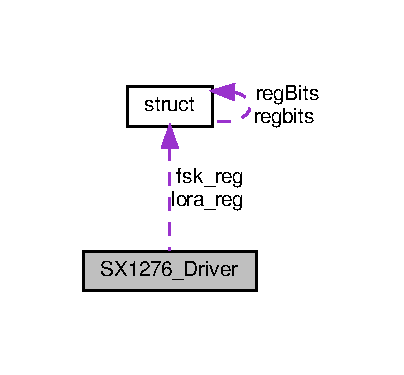
\includegraphics[width=194pt]{structSX1276__Driver__coll__graph}
\end{center}
\end{figure}
\subsection*{Public Attributes}
\begin{DoxyCompactItemize}
\item 
\mbox{\Hypertarget{structSX1276__Driver_a5701ddcbefc6cb361fc9cd0c5219bfc0}\label{structSX1276__Driver_a5701ddcbefc6cb361fc9cd0c5219bfc0}} 
sx\+\_\+device\+\_\+mode\+\_\+t {\bfseries device\+\_\+mode}
\item 
\hyperlink{structFSK__Register__Map}{F\+S\+K\+\_\+\+Register\+\_\+\+Map\+\_\+t} \hyperlink{structSX1276__Driver_af495c11033101af1032dcc76ac417492}{fsk\+\_\+reg}
\item 
\mbox{\Hypertarget{structSX1276__Driver_a2a2ded4a0e724abbefb8015bd12793af}\label{structSX1276__Driver_a2a2ded4a0e724abbefb8015bd12793af}} 
\hyperlink{structFSK__Register__Map}{Lora\+\_\+\+Register\+\_\+\+Map\+\_\+t} {\bfseries lora\+\_\+reg}
\item 
\mbox{\Hypertarget{structSX1276__Driver_aee4ec2364cc511eb360d318dbeb8152b}\label{structSX1276__Driver_aee4ec2364cc511eb360d318dbeb8152b}} 
\hyperlink{vl53l0x__types_8h_aba7bc1797add20fe3efdf37ced1182c5}{uint8\+\_\+t} {\bfseries rx\+\_\+buffer} \mbox{[}256\mbox{]}
\item 
\mbox{\Hypertarget{structSX1276__Driver_ab6f0bc93cd9588cb5911ef4613934f24}\label{structSX1276__Driver_ab6f0bc93cd9588cb5911ef4613934f24}} 
\hyperlink{vl53l0x__types_8h_aba7bc1797add20fe3efdf37ced1182c5}{uint8\+\_\+t} {\bfseries tx\+\_\+buffer} \mbox{[}256\mbox{]}
\item 
\mbox{\Hypertarget{structSX1276__Driver_ab673c55b14bec71245b4d0bd53b410ff}\label{structSX1276__Driver_ab673c55b14bec71245b4d0bd53b410ff}} 
gpio\+\_\+num\+\_\+t {\bfseries rst\+\_\+pin}
\item 
\mbox{\Hypertarget{structSX1276__Driver_a4ebc0dbd963b6262e30a63f9994111a7}\label{structSX1276__Driver_a4ebc0dbd963b6262e30a63f9994111a7}} 
gpio\+\_\+num\+\_\+t {\bfseries cs\+\_\+pin}
\item 
\mbox{\Hypertarget{structSX1276__Driver_a0e8828cf84ed41834d6d2fb025d67294}\label{structSX1276__Driver_a0e8828cf84ed41834d6d2fb025d67294}} 
spi\+\_\+device\+\_\+handle\+\_\+t {\bfseries spi\+\_\+handle}
\end{DoxyCompactItemize}


\subsection{Member Data Documentation}
\mbox{\Hypertarget{structSX1276__Driver_af495c11033101af1032dcc76ac417492}\label{structSX1276__Driver_af495c11033101af1032dcc76ac417492}} 
\index{S\+X1276\+\_\+\+Driver@{S\+X1276\+\_\+\+Driver}!fsk\+\_\+reg@{fsk\+\_\+reg}}
\index{fsk\+\_\+reg@{fsk\+\_\+reg}!S\+X1276\+\_\+\+Driver@{S\+X1276\+\_\+\+Driver}}
\subsubsection{\texorpdfstring{fsk\+\_\+reg}{fsk\_reg}}
{\footnotesize\ttfamily \hyperlink{structFSK__Register__Map}{F\+S\+K\+\_\+\+Register\+\_\+\+Map\+\_\+t} S\+X1276\+\_\+\+Driver\+::fsk\+\_\+reg}

internal register maps 

The documentation for this struct was generated from the following file\+:\begin{DoxyCompactItemize}
\item 
Lora\+S\+X1276\+\_\+\+Driver/Lora\+\_\+\+S\+X1276\+\_\+\+Driver.\+h\end{DoxyCompactItemize}

\hypertarget{structsx1276__init__t}{}\section{sx1276\+\_\+init\+\_\+t Struct Reference}
\label{structsx1276__init__t}\index{sx1276\+\_\+init\+\_\+t@{sx1276\+\_\+init\+\_\+t}}
\subsection*{Public Attributes}
\begin{DoxyCompactItemize}
\item 
\mbox{\Hypertarget{structsx1276__init__t_ab91fb4027f3653e7c4a360b11b6424aa}\label{structsx1276__init__t_ab91fb4027f3653e7c4a360b11b6424aa}} 
gpio\+\_\+num\+\_\+t {\bfseries rst\+\_\+pin}
\item 
\mbox{\Hypertarget{structsx1276__init__t_aed8d5e6f915e33bd2abc106fcb2b05e7}\label{structsx1276__init__t_aed8d5e6f915e33bd2abc106fcb2b05e7}} 
gpio\+\_\+num\+\_\+t {\bfseries cs\+\_\+pin}
\item 
\mbox{\Hypertarget{structsx1276__init__t_a4b5c8ebd9f46115d62ac9ec2789518ab}\label{structsx1276__init__t_a4b5c8ebd9f46115d62ac9ec2789518ab}} 
\hyperlink{vl53l0x__types_8h_aba7bc1797add20fe3efdf37ced1182c5}{uint8\+\_\+t} {\bfseries spi\+\_\+bus}
\end{DoxyCompactItemize}


The documentation for this struct was generated from the following file\+:\begin{DoxyCompactItemize}
\item 
Lora\+S\+X1276\+\_\+\+Driver/Lora\+\_\+\+S\+X1276\+\_\+\+Driver.\+h\end{DoxyCompactItemize}

\hypertarget{structSystemHandle}{}\section{System\+Handle Struct Reference}
\label{structSystemHandle}\index{System\+Handle@{System\+Handle}}


Collaboration diagram for System\+Handle\+:\nopagebreak
\begin{figure}[H]
\begin{center}
\leavevmode
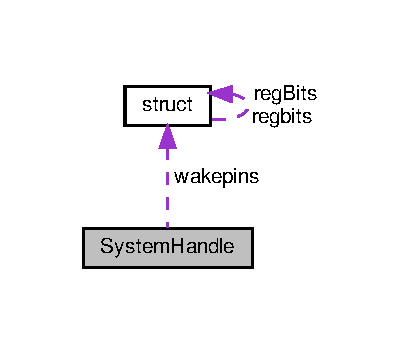
\includegraphics[width=193pt]{structSystemHandle__coll__graph}
\end{center}
\end{figure}
\subsection*{Public Attributes}
\begin{DoxyCompactItemize}
\item 
\mbox{\Hypertarget{structSystemHandle_ab28860e8cd27f2044dbfb8ddbc7cec0e}\label{structSystemHandle_ab28860e8cd27f2044dbfb8ddbc7cec0e}} 
sleepstate\+\_\+t {\bfseries sleep\+\_\+state}
\item 
\mbox{\Hypertarget{structSystemHandle_a522b36afc2050fe91d4f6ec1b9f577d5}\label{structSystemHandle_a522b36afc2050fe91d4f6ec1b9f577d5}} 
\hyperlink{vl53l0x__types_8h_a435d1572bf3f880d55459d9805097f62}{uint32\+\_\+t} {\bfseries uptime\+\_\+counter}
\item 
\mbox{\Hypertarget{structSystemHandle_a5468323d0aa250a10fb9d055b67056e6}\label{structSystemHandle_a5468323d0aa250a10fb9d055b67056e6}} 
Timer\+Handle\+\_\+t {\bfseries uptimer}
\item 
\mbox{\Hypertarget{structSystemHandle_a2c36e9ba1cee876046b1bcb694616fc0}\label{structSystemHandle_a2c36e9ba1cee876046b1bcb694616fc0}} 
\hyperlink{structWakePin}{wake\+\_\+pin\+\_\+t} {\bfseries wakepins} \mbox{[}10\mbox{]}
\item 
\mbox{\Hypertarget{structSystemHandle_a448522c01e063f5cb1e4b1331ca24e90}\label{structSystemHandle_a448522c01e063f5cb1e4b1331ca24e90}} 
\hyperlink{vl53l0x__types_8h_aba7bc1797add20fe3efdf37ced1182c5}{uint8\+\_\+t} {\bfseries no\+\_\+wakepins}
\item 
\mbox{\Hypertarget{structSystemHandle_a0518ba1247836deb986f69a79fea30ca}\label{structSystemHandle_a0518ba1247836deb986f69a79fea30ca}} 
char {\bfseries devicename} \mbox{[}32\mbox{]}
\item 
\mbox{\Hypertarget{structSystemHandle_ae58d7b6e51e8990c24a5260ecba10856}\label{structSystemHandle_ae58d7b6e51e8990c24a5260ecba10856}} 
\hyperlink{vl53l0x__types_8h_a435d1572bf3f880d55459d9805097f62}{uint32\+\_\+t} {\bfseries device\+\_\+type}
\end{DoxyCompactItemize}


The documentation for this struct was generated from the following file\+:\begin{DoxyCompactItemize}
\item 
Systerm\+Component/System\+Component.\+h\end{DoxyCompactItemize}

\hypertarget{structThe}{}\section{The Struct Reference}
\label{structThe}\index{The@{The}}


Contains the information used to intialise the driver.  




\subsection{Detailed Description}
Contains the information used to intialise the driver. 

structure 

The documentation for this struct was generated from the following file\+:\begin{DoxyCompactItemize}
\item 
A\+P\+A102\+\_\+\+Driver/A\+P\+A102\+\_\+\+Driver.\+h\end{DoxyCompactItemize}

\hypertarget{structTouchSenseDriver}{}\section{Touch\+Sense\+Driver Struct Reference}
\label{structTouchSenseDriver}\index{Touch\+Sense\+Driver@{Touch\+Sense\+Driver}}
\subsection*{Public Attributes}
\begin{DoxyCompactItemize}
\item 
\mbox{\Hypertarget{structTouchSenseDriver_a3fd5371d89f1eaf7cfb72ef10dfa1de3}\label{structTouchSenseDriver_a3fd5371d89f1eaf7cfb72ef10dfa1de3}} 
gpio\+\_\+num\+\_\+t {\bfseries touch\+\_\+pins} \mbox{[}T\+O\+U\+C\+H\+S\+E\+N\+S\+E\+\_\+\+M\+A\+X\+\_\+\+P\+I\+NS\mbox{]}
\item 
\mbox{\Hypertarget{structTouchSenseDriver_aac16471c093be72b63e8b2e0dc48f791}\label{structTouchSenseDriver_aac16471c093be72b63e8b2e0dc48f791}} 
\hyperlink{vl53l0x__types_8h_aba7bc1797add20fe3efdf37ced1182c5}{uint8\+\_\+t} {\bfseries num\+\_\+pins}
\item 
\mbox{\Hypertarget{structTouchSenseDriver_a0769e6c179073d6fd46560921521972b}\label{structTouchSenseDriver_a0769e6c179073d6fd46560921521972b}} 
Task\+Handle\+\_\+t {\bfseries t\+\_\+handle}
\item 
\mbox{\Hypertarget{structTouchSenseDriver_ab62b350c5ff94babe305db8db759a114}\label{structTouchSenseDriver_ab62b350c5ff94babe305db8db759a114}} 
Timer\+Handle\+\_\+t {\bfseries timer}
\end{DoxyCompactItemize}


The documentation for this struct was generated from the following file\+:\begin{DoxyCompactItemize}
\item 
Utils/Touch\+Sense\+Driver.\+h\end{DoxyCompactItemize}

\hypertarget{structTouchSenseInit}{}\section{Touch\+Sense\+Init Struct Reference}
\label{structTouchSenseInit}\index{Touch\+Sense\+Init@{Touch\+Sense\+Init}}
\subsection*{Public Attributes}
\begin{DoxyCompactItemize}
\item 
\mbox{\Hypertarget{structTouchSenseInit_a319ec86281c796d47b341c8fda47ff62}\label{structTouchSenseInit_a319ec86281c796d47b341c8fda47ff62}} 
gpio\+\_\+num\+\_\+t {\bfseries touch\+\_\+pins} \mbox{[}T\+O\+U\+C\+H\+S\+E\+N\+S\+E\+\_\+\+M\+A\+X\+\_\+\+P\+I\+NS\mbox{]}
\item 
\mbox{\Hypertarget{structTouchSenseInit_ac4be7a6e1d38e3ddf71fa3c4ab7f9666}\label{structTouchSenseInit_ac4be7a6e1d38e3ddf71fa3c4ab7f9666}} 
\hyperlink{vl53l0x__types_8h_aba7bc1797add20fe3efdf37ced1182c5}{uint8\+\_\+t} {\bfseries num\+\_\+pins}
\item 
\mbox{\Hypertarget{structTouchSenseInit_a1034ab71d367c6838e3adef5d34679b0}\label{structTouchSenseInit_a1034ab71d367c6838e3adef5d34679b0}} 
void $\ast$ {\bfseries event\+\_\+loop}
\end{DoxyCompactItemize}


The documentation for this struct was generated from the following file\+:\begin{DoxyCompactItemize}
\item 
Utils/Touch\+Sense\+Driver.\+h\end{DoxyCompactItemize}

\hypertarget{structVEML6070__Driver}{}\section{V\+E\+M\+L6070\+\_\+\+Driver Struct Reference}
\label{structVEML6070__Driver}\index{V\+E\+M\+L6070\+\_\+\+Driver@{V\+E\+M\+L6070\+\_\+\+Driver}}
\subsection*{Public Attributes}
\begin{DoxyCompactItemize}
\item 
\mbox{\Hypertarget{structVEML6070__Driver_a8efe47c65d7bf944e38fc12ec28932ec}\label{structVEML6070__Driver_a8efe47c65d7bf944e38fc12ec28932ec}} 
\hyperlink{vl53l0x__types_8h_aba7bc1797add20fe3efdf37ced1182c5}{uint8\+\_\+t} {\bfseries bus}
\item 
\mbox{\Hypertarget{structVEML6070__Driver_af1c9e7fefec6867ce382149308ad1b6c}\label{structVEML6070__Driver_af1c9e7fefec6867ce382149308ad1b6c}} 
gpio\+\_\+num\+\_\+t {\bfseries ack}
\item 
\mbox{\Hypertarget{structVEML6070__Driver_a623862e8164bee7cce40d52dde10d0b3}\label{structVEML6070__Driver_a623862e8164bee7cce40d52dde10d0b3}} 
bool {\bfseries intr\+\_\+en}
\item 
\mbox{\Hypertarget{structVEML6070__Driver_a087acac12be67f20a6c1e89ead639c9f}\label{structVEML6070__Driver_a087acac12be67f20a6c1e89ead639c9f}} 
Task\+Handle\+\_\+t {\bfseries task}
\item 
\mbox{\Hypertarget{structVEML6070__Driver_a356684f4cd4468183ae7cd74b4e69e8a}\label{structVEML6070__Driver_a356684f4cd4468183ae7cd74b4e69e8a}} 
veml\+\_\+state\+\_\+t {\bfseries state}
\item 
\mbox{\Hypertarget{structVEML6070__Driver_ab40a8e69273ef222a8e63e6e39cf7931}\label{structVEML6070__Driver_ab40a8e69273ef222a8e63e6e39cf7931}} 
\hyperlink{vl53l0x__types_8h_a273cf69d639a59973b6019625df33e30}{uint16\+\_\+t} {\bfseries last\+\_\+value}
\end{DoxyCompactItemize}


The documentation for this struct was generated from the following file\+:\begin{DoxyCompactItemize}
\item 
V\+E\+M\+L6070\+\_\+\+Driver/V\+E\+M\+L6070\+\_\+\+Driver.\+h\end{DoxyCompactItemize}

\hypertarget{structveml__init}{}\section{veml\+\_\+init Struct Reference}
\label{structveml__init}\index{veml\+\_\+init@{veml\+\_\+init}}
\subsection*{Public Attributes}
\begin{DoxyCompactItemize}
\item 
\mbox{\Hypertarget{structveml__init_affe921782a5def8805ff4937d5d65d89}\label{structveml__init_affe921782a5def8805ff4937d5d65d89}} 
\hyperlink{vl53l0x__types_8h_aba7bc1797add20fe3efdf37ced1182c5}{uint8\+\_\+t} {\bfseries i2c\+\_\+bus}
\item 
\mbox{\Hypertarget{structveml__init_ab2752cd05e20a5b71f0f15b2d898e2b7}\label{structveml__init_ab2752cd05e20a5b71f0f15b2d898e2b7}} 
gpio\+\_\+num\+\_\+t {\bfseries ack\+\_\+pin}
\end{DoxyCompactItemize}


The documentation for this struct was generated from the following file\+:\begin{DoxyCompactItemize}
\item 
V\+E\+M\+L6070\+\_\+\+Driver/V\+E\+M\+L6070\+\_\+\+Driver.\+h\end{DoxyCompactItemize}

\hypertarget{structVFD__Init}{}\section{V\+F\+D\+\_\+\+Init Struct Reference}
\label{structVFD__Init}\index{V\+F\+D\+\_\+\+Init@{V\+F\+D\+\_\+\+Init}}
\subsection*{Public Attributes}
\begin{DoxyCompactItemize}
\item 
\mbox{\Hypertarget{structVFD__Init_a11373a800afc912159f5234dc5d3a4a1}\label{structVFD__Init_a11373a800afc912159f5234dc5d3a4a1}} 
\hyperlink{vl53l0x__types_8h_aba7bc1797add20fe3efdf37ced1182c5}{uint8\+\_\+t} {\bfseries spi\+\_\+bus}
\item 
\mbox{\Hypertarget{structVFD__Init_a48d6d57a79c4658692127c5fb42c97fc}\label{structVFD__Init_a48d6d57a79c4658692127c5fb42c97fc}} 
\hyperlink{vl53l0x__types_8h_a273cf69d639a59973b6019625df33e30}{uint16\+\_\+t} {\bfseries clock\+\_\+speed}
\item 
\mbox{\Hypertarget{structVFD__Init_aa00735627b22df6811c65d98d95dec4c}\label{structVFD__Init_aa00735627b22df6811c65d98d95dec4c}} 
gpio\+\_\+num\+\_\+t {\bfseries cs\+\_\+pin}
\item 
\mbox{\Hypertarget{structVFD__Init_ace7aabc2a7ec3baa3c5691013e057d48}\label{structVFD__Init_ace7aabc2a7ec3baa3c5691013e057d48}} 
gpio\+\_\+num\+\_\+t {\bfseries rst\+\_\+pin}
\end{DoxyCompactItemize}


The documentation for this struct was generated from the following file\+:\begin{DoxyCompactItemize}
\item 
Futaba\+V\+F\+D\+\_\+\+Driver/Futaba\+V\+F\+D\+\_\+\+Driver.\+h\end{DoxyCompactItemize}

\hypertarget{structVL53L0X__Dev__t}{}\section{V\+L53\+L0\+X\+\_\+\+Dev\+\_\+t Struct Reference}
\label{structVL53L0X__Dev__t}\index{V\+L53\+L0\+X\+\_\+\+Dev\+\_\+t@{V\+L53\+L0\+X\+\_\+\+Dev\+\_\+t}}


Generic P\+AL device type that does link between A\+PI and platform abstraction layer.  




{\ttfamily \#include $<$vl53l0x\+\_\+platform.\+h$>$}



Collaboration diagram for V\+L53\+L0\+X\+\_\+\+Dev\+\_\+t\+:\nopagebreak
\begin{figure}[H]
\begin{center}
\leavevmode
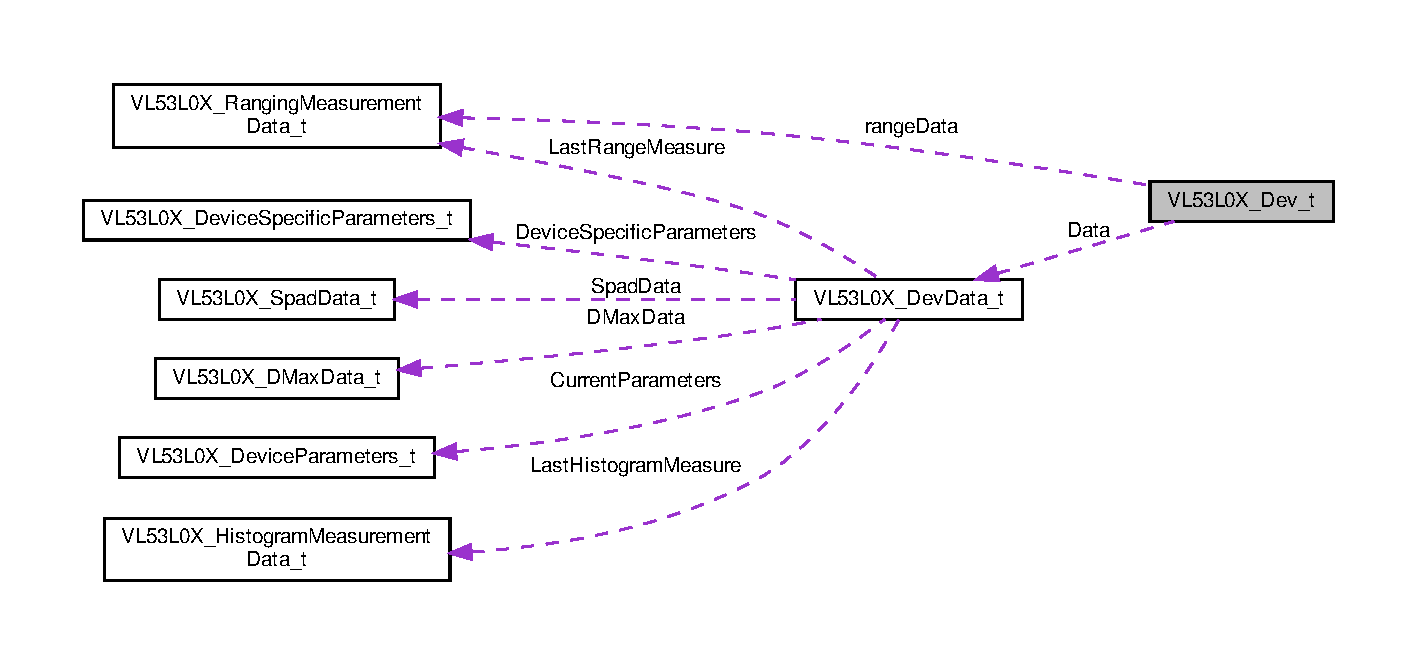
\includegraphics[width=350pt]{structVL53L0X__Dev__t__coll__graph}
\end{center}
\end{figure}
\subsection*{Public Attributes}
\begin{DoxyCompactItemize}
\item 
\hyperlink{structVL53L0X__DevData__t}{V\+L53\+L0\+X\+\_\+\+Dev\+Data\+\_\+t} \hyperlink{structVL53L0X__Dev__t_ab69036a33cb4bfdf295d53e1ab15ff54}{Data}
\item 
\hyperlink{vl53l0x__types_8h_aba7bc1797add20fe3efdf37ced1182c5}{uint8\+\_\+t} \hyperlink{structVL53L0X__Dev__t_add69f3fe32d5d1fc063133763a282e2c}{I2c\+Dev\+Addr}
\item 
\hyperlink{vl53l0x__types_8h_aba7bc1797add20fe3efdf37ced1182c5}{uint8\+\_\+t} \hyperlink{structVL53L0X__Dev__t_ad31ab98c8e3f4461d322f1089430e714}{comms\+\_\+type}
\item 
\hyperlink{vl53l0x__types_8h_a273cf69d639a59973b6019625df33e30}{uint16\+\_\+t} \hyperlink{structVL53L0X__Dev__t_a7aff2b204283beb1e5a73f887c8cceb9}{comms\+\_\+speed\+\_\+khz}
\item 
V\+L53\+L0\+X\+\_\+\+Device\+Modes \hyperlink{structVL53L0X__Dev__t_a1a823e2387e3fa81bae5a1412ed52384}{dev\+\_\+mode}
\item 
\mbox{\Hypertarget{structVL53L0X__Dev__t_aa1773c06fb519cdcc3391fd213e015e5}\label{structVL53L0X__Dev__t_aa1773c06fb519cdcc3391fd213e015e5}} 
\hyperlink{structVL53L0X__RangingMeasurementData__t}{V\+L53\+L0\+X\+\_\+\+Ranging\+Measurement\+Data\+\_\+t} {\bfseries range\+Data}
\item 
\mbox{\Hypertarget{structVL53L0X__Dev__t_a3dea4228d57eaf99d536f800984b98d6}\label{structVL53L0X__Dev__t_a3dea4228d57eaf99d536f800984b98d6}} 
V\+L53\+L0\+X\+\_\+config\+\_\+t {\bfseries sample\+\_\+mode}
\end{DoxyCompactItemize}


\subsection{Detailed Description}
Generic P\+AL device type that does link between A\+PI and platform abstraction layer. 

\subsection{Member Data Documentation}
\mbox{\Hypertarget{structVL53L0X__Dev__t_a7aff2b204283beb1e5a73f887c8cceb9}\label{structVL53L0X__Dev__t_a7aff2b204283beb1e5a73f887c8cceb9}} 
\index{V\+L53\+L0\+X\+\_\+\+Dev\+\_\+t@{V\+L53\+L0\+X\+\_\+\+Dev\+\_\+t}!comms\+\_\+speed\+\_\+khz@{comms\+\_\+speed\+\_\+khz}}
\index{comms\+\_\+speed\+\_\+khz@{comms\+\_\+speed\+\_\+khz}!V\+L53\+L0\+X\+\_\+\+Dev\+\_\+t@{V\+L53\+L0\+X\+\_\+\+Dev\+\_\+t}}
\subsubsection{\texorpdfstring{comms\+\_\+speed\+\_\+khz}{comms\_speed\_khz}}
{\footnotesize\ttfamily \hyperlink{vl53l0x__types_8h_a273cf69d639a59973b6019625df33e30}{uint16\+\_\+t} V\+L53\+L0\+X\+\_\+\+Dev\+\_\+t\+::comms\+\_\+speed\+\_\+khz}

Comms speed \mbox{[}k\+Hz\mbox{]} \+: typically 400k\+Hz for I2C \mbox{\Hypertarget{structVL53L0X__Dev__t_ad31ab98c8e3f4461d322f1089430e714}\label{structVL53L0X__Dev__t_ad31ab98c8e3f4461d322f1089430e714}} 
\index{V\+L53\+L0\+X\+\_\+\+Dev\+\_\+t@{V\+L53\+L0\+X\+\_\+\+Dev\+\_\+t}!comms\+\_\+type@{comms\+\_\+type}}
\index{comms\+\_\+type@{comms\+\_\+type}!V\+L53\+L0\+X\+\_\+\+Dev\+\_\+t@{V\+L53\+L0\+X\+\_\+\+Dev\+\_\+t}}
\subsubsection{\texorpdfstring{comms\+\_\+type}{comms\_type}}
{\footnotesize\ttfamily \hyperlink{vl53l0x__types_8h_aba7bc1797add20fe3efdf37ced1182c5}{uint8\+\_\+t} V\+L53\+L0\+X\+\_\+\+Dev\+\_\+t\+::comms\+\_\+type}

Type of comms \+: V\+L53\+L0\+X\+\_\+\+C\+O\+M\+M\+S\+\_\+\+I2C or V\+L53\+L0\+X\+\_\+\+C\+O\+M\+M\+S\+\_\+\+S\+PI \mbox{\Hypertarget{structVL53L0X__Dev__t_ab69036a33cb4bfdf295d53e1ab15ff54}\label{structVL53L0X__Dev__t_ab69036a33cb4bfdf295d53e1ab15ff54}} 
\index{V\+L53\+L0\+X\+\_\+\+Dev\+\_\+t@{V\+L53\+L0\+X\+\_\+\+Dev\+\_\+t}!Data@{Data}}
\index{Data@{Data}!V\+L53\+L0\+X\+\_\+\+Dev\+\_\+t@{V\+L53\+L0\+X\+\_\+\+Dev\+\_\+t}}
\subsubsection{\texorpdfstring{Data}{Data}}
{\footnotesize\ttfamily \hyperlink{structVL53L0X__DevData__t}{V\+L53\+L0\+X\+\_\+\+Dev\+Data\+\_\+t} V\+L53\+L0\+X\+\_\+\+Dev\+\_\+t\+::\+Data}

embed ST Ewok Dev data as \char`\"{}\+Data\char`\"{} user specific field \mbox{\Hypertarget{structVL53L0X__Dev__t_a1a823e2387e3fa81bae5a1412ed52384}\label{structVL53L0X__Dev__t_a1a823e2387e3fa81bae5a1412ed52384}} 
\index{V\+L53\+L0\+X\+\_\+\+Dev\+\_\+t@{V\+L53\+L0\+X\+\_\+\+Dev\+\_\+t}!dev\+\_\+mode@{dev\+\_\+mode}}
\index{dev\+\_\+mode@{dev\+\_\+mode}!V\+L53\+L0\+X\+\_\+\+Dev\+\_\+t@{V\+L53\+L0\+X\+\_\+\+Dev\+\_\+t}}
\subsubsection{\texorpdfstring{dev\+\_\+mode}{dev\_mode}}
{\footnotesize\ttfamily V\+L53\+L0\+X\+\_\+\+Device\+Modes V\+L53\+L0\+X\+\_\+\+Dev\+\_\+t\+::dev\+\_\+mode}

current device mode \mbox{\Hypertarget{structVL53L0X__Dev__t_add69f3fe32d5d1fc063133763a282e2c}\label{structVL53L0X__Dev__t_add69f3fe32d5d1fc063133763a282e2c}} 
\index{V\+L53\+L0\+X\+\_\+\+Dev\+\_\+t@{V\+L53\+L0\+X\+\_\+\+Dev\+\_\+t}!I2c\+Dev\+Addr@{I2c\+Dev\+Addr}}
\index{I2c\+Dev\+Addr@{I2c\+Dev\+Addr}!V\+L53\+L0\+X\+\_\+\+Dev\+\_\+t@{V\+L53\+L0\+X\+\_\+\+Dev\+\_\+t}}
\subsubsection{\texorpdfstring{I2c\+Dev\+Addr}{I2cDevAddr}}
{\footnotesize\ttfamily \hyperlink{vl53l0x__types_8h_aba7bc1797add20fe3efdf37ced1182c5}{uint8\+\_\+t} V\+L53\+L0\+X\+\_\+\+Dev\+\_\+t\+::\+I2c\+Dev\+Addr}

i2c device address user specific field 

The documentation for this struct was generated from the following file\+:\begin{DoxyCompactItemize}
\item 
V\+L53\+L0\+X\+\_\+\+Driver/\+V\+L53\+L0\+X/include/\hyperlink{vl53l0x__platform_8h}{vl53l0x\+\_\+platform.\+h}\end{DoxyCompactItemize}

\hypertarget{structVL53L0X__DevData__t}{}\section{V\+L53\+L0\+X\+\_\+\+Dev\+Data\+\_\+t Struct Reference}
\label{structVL53L0X__DevData__t}\index{V\+L53\+L0\+X\+\_\+\+Dev\+Data\+\_\+t@{V\+L53\+L0\+X\+\_\+\+Dev\+Data\+\_\+t}}


V\+L53\+L0X P\+AL device ST private data structure ~\newline
End user should never access any of these field directly.  




{\ttfamily \#include $<$vl53l0x\+\_\+def.\+h$>$}



Collaboration diagram for V\+L53\+L0\+X\+\_\+\+Dev\+Data\+\_\+t\+:\nopagebreak
\begin{figure}[H]
\begin{center}
\leavevmode
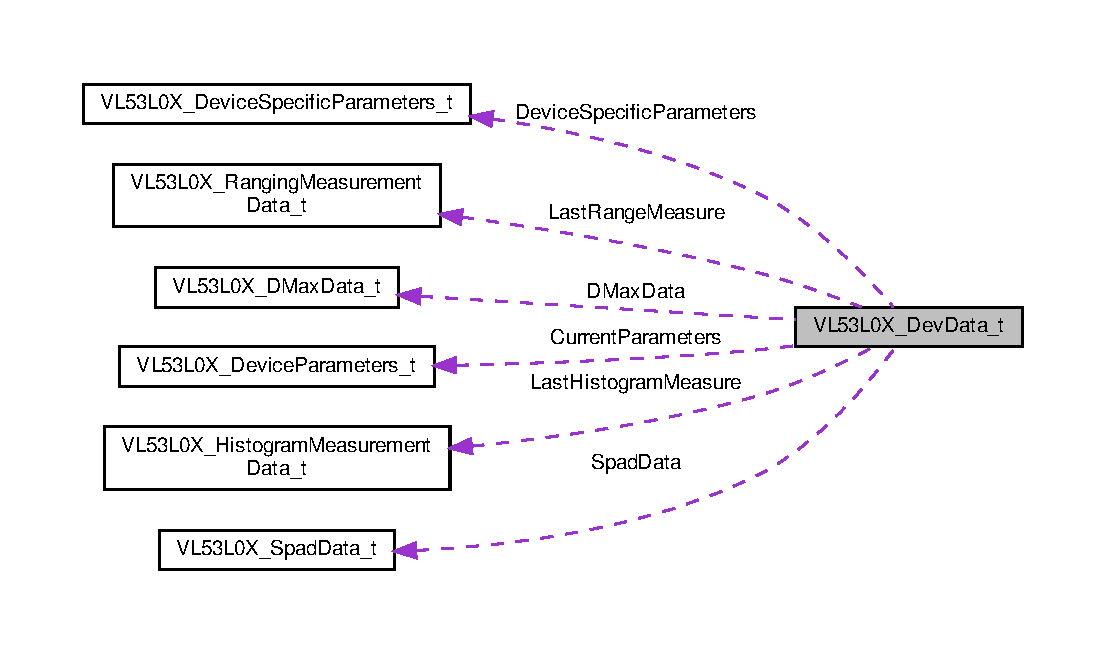
\includegraphics[width=350pt]{structVL53L0X__DevData__t__coll__graph}
\end{center}
\end{figure}
\subsection*{Public Attributes}
\begin{DoxyCompactItemize}
\item 
\hyperlink{structVL53L0X__DMaxData__t}{V\+L53\+L0\+X\+\_\+\+D\+Max\+Data\+\_\+t} \hyperlink{structVL53L0X__DevData__t_a2acc06ceafef9afc6687aa9216fffb66}{D\+Max\+Data}
\item 
\hyperlink{vl53l0x__types_8h_a32f2e37ee053cf2ce8ca28d1f74630e5}{int32\+\_\+t} \hyperlink{structVL53L0X__DevData__t_aab25fa7eaf3170a3b510cbe4abc63e99}{Part2\+Part\+Offset\+N\+V\+M\+Micro\+Meter}
\item 
\hyperlink{vl53l0x__types_8h_a32f2e37ee053cf2ce8ca28d1f74630e5}{int32\+\_\+t} \hyperlink{structVL53L0X__DevData__t_a0853140c55bf2320db3881a42226bbd7}{Part2\+Part\+Offset\+Adjustment\+N\+V\+M\+Micro\+Meter}
\item 
\hyperlink{structVL53L0X__DeviceParameters__t}{V\+L53\+L0\+X\+\_\+\+Device\+Parameters\+\_\+t} \hyperlink{structVL53L0X__DevData__t_a823d3a952c645f472c3130e7f956f0e1}{Current\+Parameters}
\item 
\hyperlink{structVL53L0X__RangingMeasurementData__t}{V\+L53\+L0\+X\+\_\+\+Ranging\+Measurement\+Data\+\_\+t} \hyperlink{structVL53L0X__DevData__t_aab812161cf71d2ad654e4d3491162221}{Last\+Range\+Measure}
\item 
\hyperlink{structVL53L0X__HistogramMeasurementData__t}{V\+L53\+L0\+X\+\_\+\+Histogram\+Measurement\+Data\+\_\+t} \hyperlink{structVL53L0X__DevData__t_a957c038c2009bd4ea69081ea324f9bf4}{Last\+Histogram\+Measure}
\item 
\hyperlink{structVL53L0X__DeviceSpecificParameters__t}{V\+L53\+L0\+X\+\_\+\+Device\+Specific\+Parameters\+\_\+t} \hyperlink{structVL53L0X__DevData__t_a0f50334a87083360b8c97073a4edd364}{Device\+Specific\+Parameters}
\item 
\hyperlink{structVL53L0X__SpadData__t}{V\+L53\+L0\+X\+\_\+\+Spad\+Data\+\_\+t} \hyperlink{structVL53L0X__DevData__t_a5d1c5466b9220e5253d8890a5cb9e0a7}{Spad\+Data}
\item 
\hyperlink{vl53l0x__types_8h_aba7bc1797add20fe3efdf37ced1182c5}{uint8\+\_\+t} \hyperlink{structVL53L0X__DevData__t_abe609c057515be9541a1776746364fd3}{Sequence\+Config}
\item 
\hyperlink{vl53l0x__types_8h_aba7bc1797add20fe3efdf37ced1182c5}{uint8\+\_\+t} \hyperlink{structVL53L0X__DevData__t_ad5a07400adf4a6daf9e1278cb2f68de1}{Range\+Fractional\+Enable}
\item 
V\+L53\+L0\+X\+\_\+\+State \hyperlink{structVL53L0X__DevData__t_a2af2f91ed84e2f07ec4349ab4a51c254}{Pal\+State}
\item 
V\+L53\+L0\+X\+\_\+\+Power\+Modes \hyperlink{structVL53L0X__DevData__t_acdedec2043594afca8ea4e31af87b44b}{Power\+Mode}
\item 
\hyperlink{vl53l0x__types_8h_a273cf69d639a59973b6019625df33e30}{uint16\+\_\+t} \hyperlink{structVL53L0X__DevData__t_a88d3c2b890dd076df712c173c608c27d}{Sigma\+Est\+Ref\+Array}
\item 
\hyperlink{vl53l0x__types_8h_a273cf69d639a59973b6019625df33e30}{uint16\+\_\+t} \hyperlink{structVL53L0X__DevData__t_ab0f319430e08b3362daa62749de409ac}{Sigma\+Est\+Eff\+Pulse\+Width}
\item 
\hyperlink{vl53l0x__types_8h_a273cf69d639a59973b6019625df33e30}{uint16\+\_\+t} \hyperlink{structVL53L0X__DevData__t_acb01571c3ab7f02974882547a24778de}{Sigma\+Est\+Eff\+Amb\+Width}
\item 
\hyperlink{vl53l0x__types_8h_aba7bc1797add20fe3efdf37ced1182c5}{uint8\+\_\+t} \hyperlink{structVL53L0X__DevData__t_aa899dbe8e0c83e0115418f67ad320476}{Stop\+Variable}
\item 
\hyperlink{vl53l0x__types_8h_a273cf69d639a59973b6019625df33e30}{uint16\+\_\+t} \hyperlink{structVL53L0X__DevData__t_adfd2ebd6ffbb3e0d6b6f215f43acaf70}{target\+Ref\+Rate}
\item 
\hyperlink{vl53l0x__types_8h_afb910790161809fc76e1a274a6349384}{Fix\+Point1616\+\_\+t} \hyperlink{structVL53L0X__DevData__t_a6a7882154860331aa2cde829124a1b28}{Sigma\+Estimate}
\item 
\hyperlink{vl53l0x__types_8h_afb910790161809fc76e1a274a6349384}{Fix\+Point1616\+\_\+t} \hyperlink{structVL53L0X__DevData__t_aef67fd52e16bb8ce1af82411d39076b2}{Signal\+Estimate}
\item 
\hyperlink{vl53l0x__types_8h_afb910790161809fc76e1a274a6349384}{Fix\+Point1616\+\_\+t} \hyperlink{structVL53L0X__DevData__t_a3a6ffec0ee4b3f6a150012badc4a7b2f}{Last\+Signal\+Ref\+Mcps}
\item 
\hyperlink{vl53l0x__types_8h_aba7bc1797add20fe3efdf37ced1182c5}{uint8\+\_\+t} $\ast$ \hyperlink{structVL53L0X__DevData__t_add6d178727ef03670b8b750eff3bd482}{p\+Tuning\+Settings\+Pointer}
\item 
\hyperlink{vl53l0x__types_8h_aba7bc1797add20fe3efdf37ced1182c5}{uint8\+\_\+t} \hyperlink{structVL53L0X__DevData__t_af639b5aecb7430bef08d614a2a65a059}{Use\+Internal\+Tuning\+Settings}
\item 
\hyperlink{vl53l0x__types_8h_a273cf69d639a59973b6019625df33e30}{uint16\+\_\+t} \hyperlink{structVL53L0X__DevData__t_ac30c7ce4262f144af814f9665c0d1f60}{Linearity\+Corrective\+Gain}
\item 
\hyperlink{vl53l0x__types_8h_a273cf69d639a59973b6019625df33e30}{uint16\+\_\+t} \hyperlink{structVL53L0X__DevData__t_a25258ff806f25c9ea91012fd9b69dc46}{Dmax\+Cal\+Range\+Milli\+Meter}
\item 
\hyperlink{vl53l0x__types_8h_afb910790161809fc76e1a274a6349384}{Fix\+Point1616\+\_\+t} \hyperlink{structVL53L0X__DevData__t_a564bb3bd87e8950734a5d99d121313d0}{Dmax\+Cal\+Signal\+Rate\+Rtn\+Mega\+Cps}
\end{DoxyCompactItemize}


\subsection{Detailed Description}
V\+L53\+L0X P\+AL device ST private data structure ~\newline
End user should never access any of these field directly. 

These must never access directly but only via macro 

\subsection{Member Data Documentation}
\mbox{\Hypertarget{structVL53L0X__DevData__t_a823d3a952c645f472c3130e7f956f0e1}\label{structVL53L0X__DevData__t_a823d3a952c645f472c3130e7f956f0e1}} 
\index{V\+L53\+L0\+X\+\_\+\+Dev\+Data\+\_\+t@{V\+L53\+L0\+X\+\_\+\+Dev\+Data\+\_\+t}!Current\+Parameters@{Current\+Parameters}}
\index{Current\+Parameters@{Current\+Parameters}!V\+L53\+L0\+X\+\_\+\+Dev\+Data\+\_\+t@{V\+L53\+L0\+X\+\_\+\+Dev\+Data\+\_\+t}}
\subsubsection{\texorpdfstring{Current\+Parameters}{CurrentParameters}}
{\footnotesize\ttfamily \hyperlink{structVL53L0X__DeviceParameters__t}{V\+L53\+L0\+X\+\_\+\+Device\+Parameters\+\_\+t} V\+L53\+L0\+X\+\_\+\+Dev\+Data\+\_\+t\+::\+Current\+Parameters}

Current Device Parameter \mbox{\Hypertarget{structVL53L0X__DevData__t_a0f50334a87083360b8c97073a4edd364}\label{structVL53L0X__DevData__t_a0f50334a87083360b8c97073a4edd364}} 
\index{V\+L53\+L0\+X\+\_\+\+Dev\+Data\+\_\+t@{V\+L53\+L0\+X\+\_\+\+Dev\+Data\+\_\+t}!Device\+Specific\+Parameters@{Device\+Specific\+Parameters}}
\index{Device\+Specific\+Parameters@{Device\+Specific\+Parameters}!V\+L53\+L0\+X\+\_\+\+Dev\+Data\+\_\+t@{V\+L53\+L0\+X\+\_\+\+Dev\+Data\+\_\+t}}
\subsubsection{\texorpdfstring{Device\+Specific\+Parameters}{DeviceSpecificParameters}}
{\footnotesize\ttfamily \hyperlink{structVL53L0X__DeviceSpecificParameters__t}{V\+L53\+L0\+X\+\_\+\+Device\+Specific\+Parameters\+\_\+t} V\+L53\+L0\+X\+\_\+\+Dev\+Data\+\_\+t\+::\+Device\+Specific\+Parameters}

Parameters specific to the device \mbox{\Hypertarget{structVL53L0X__DevData__t_a25258ff806f25c9ea91012fd9b69dc46}\label{structVL53L0X__DevData__t_a25258ff806f25c9ea91012fd9b69dc46}} 
\index{V\+L53\+L0\+X\+\_\+\+Dev\+Data\+\_\+t@{V\+L53\+L0\+X\+\_\+\+Dev\+Data\+\_\+t}!Dmax\+Cal\+Range\+Milli\+Meter@{Dmax\+Cal\+Range\+Milli\+Meter}}
\index{Dmax\+Cal\+Range\+Milli\+Meter@{Dmax\+Cal\+Range\+Milli\+Meter}!V\+L53\+L0\+X\+\_\+\+Dev\+Data\+\_\+t@{V\+L53\+L0\+X\+\_\+\+Dev\+Data\+\_\+t}}
\subsubsection{\texorpdfstring{Dmax\+Cal\+Range\+Milli\+Meter}{DmaxCalRangeMilliMeter}}
{\footnotesize\ttfamily \hyperlink{vl53l0x__types_8h_a273cf69d639a59973b6019625df33e30}{uint16\+\_\+t} V\+L53\+L0\+X\+\_\+\+Dev\+Data\+\_\+t\+::\+Dmax\+Cal\+Range\+Milli\+Meter}

Dmax Calibration Range millimeter \mbox{\Hypertarget{structVL53L0X__DevData__t_a564bb3bd87e8950734a5d99d121313d0}\label{structVL53L0X__DevData__t_a564bb3bd87e8950734a5d99d121313d0}} 
\index{V\+L53\+L0\+X\+\_\+\+Dev\+Data\+\_\+t@{V\+L53\+L0\+X\+\_\+\+Dev\+Data\+\_\+t}!Dmax\+Cal\+Signal\+Rate\+Rtn\+Mega\+Cps@{Dmax\+Cal\+Signal\+Rate\+Rtn\+Mega\+Cps}}
\index{Dmax\+Cal\+Signal\+Rate\+Rtn\+Mega\+Cps@{Dmax\+Cal\+Signal\+Rate\+Rtn\+Mega\+Cps}!V\+L53\+L0\+X\+\_\+\+Dev\+Data\+\_\+t@{V\+L53\+L0\+X\+\_\+\+Dev\+Data\+\_\+t}}
\subsubsection{\texorpdfstring{Dmax\+Cal\+Signal\+Rate\+Rtn\+Mega\+Cps}{DmaxCalSignalRateRtnMegaCps}}
{\footnotesize\ttfamily \hyperlink{vl53l0x__types_8h_afb910790161809fc76e1a274a6349384}{Fix\+Point1616\+\_\+t} V\+L53\+L0\+X\+\_\+\+Dev\+Data\+\_\+t\+::\+Dmax\+Cal\+Signal\+Rate\+Rtn\+Mega\+Cps}

Dmax Calibration Signal Rate Return Mega\+Cps \mbox{\Hypertarget{structVL53L0X__DevData__t_a2acc06ceafef9afc6687aa9216fffb66}\label{structVL53L0X__DevData__t_a2acc06ceafef9afc6687aa9216fffb66}} 
\index{V\+L53\+L0\+X\+\_\+\+Dev\+Data\+\_\+t@{V\+L53\+L0\+X\+\_\+\+Dev\+Data\+\_\+t}!D\+Max\+Data@{D\+Max\+Data}}
\index{D\+Max\+Data@{D\+Max\+Data}!V\+L53\+L0\+X\+\_\+\+Dev\+Data\+\_\+t@{V\+L53\+L0\+X\+\_\+\+Dev\+Data\+\_\+t}}
\subsubsection{\texorpdfstring{D\+Max\+Data}{DMaxData}}
{\footnotesize\ttfamily \hyperlink{structVL53L0X__DMaxData__t}{V\+L53\+L0\+X\+\_\+\+D\+Max\+Data\+\_\+t} V\+L53\+L0\+X\+\_\+\+Dev\+Data\+\_\+t\+::\+D\+Max\+Data}

Dmax Data \mbox{\Hypertarget{structVL53L0X__DevData__t_a957c038c2009bd4ea69081ea324f9bf4}\label{structVL53L0X__DevData__t_a957c038c2009bd4ea69081ea324f9bf4}} 
\index{V\+L53\+L0\+X\+\_\+\+Dev\+Data\+\_\+t@{V\+L53\+L0\+X\+\_\+\+Dev\+Data\+\_\+t}!Last\+Histogram\+Measure@{Last\+Histogram\+Measure}}
\index{Last\+Histogram\+Measure@{Last\+Histogram\+Measure}!V\+L53\+L0\+X\+\_\+\+Dev\+Data\+\_\+t@{V\+L53\+L0\+X\+\_\+\+Dev\+Data\+\_\+t}}
\subsubsection{\texorpdfstring{Last\+Histogram\+Measure}{LastHistogramMeasure}}
{\footnotesize\ttfamily \hyperlink{structVL53L0X__HistogramMeasurementData__t}{V\+L53\+L0\+X\+\_\+\+Histogram\+Measurement\+Data\+\_\+t} V\+L53\+L0\+X\+\_\+\+Dev\+Data\+\_\+t\+::\+Last\+Histogram\+Measure}

Histogram Data \mbox{\Hypertarget{structVL53L0X__DevData__t_aab812161cf71d2ad654e4d3491162221}\label{structVL53L0X__DevData__t_aab812161cf71d2ad654e4d3491162221}} 
\index{V\+L53\+L0\+X\+\_\+\+Dev\+Data\+\_\+t@{V\+L53\+L0\+X\+\_\+\+Dev\+Data\+\_\+t}!Last\+Range\+Measure@{Last\+Range\+Measure}}
\index{Last\+Range\+Measure@{Last\+Range\+Measure}!V\+L53\+L0\+X\+\_\+\+Dev\+Data\+\_\+t@{V\+L53\+L0\+X\+\_\+\+Dev\+Data\+\_\+t}}
\subsubsection{\texorpdfstring{Last\+Range\+Measure}{LastRangeMeasure}}
{\footnotesize\ttfamily \hyperlink{structVL53L0X__RangingMeasurementData__t}{V\+L53\+L0\+X\+\_\+\+Ranging\+Measurement\+Data\+\_\+t} V\+L53\+L0\+X\+\_\+\+Dev\+Data\+\_\+t\+::\+Last\+Range\+Measure}

Ranging Data \mbox{\Hypertarget{structVL53L0X__DevData__t_a3a6ffec0ee4b3f6a150012badc4a7b2f}\label{structVL53L0X__DevData__t_a3a6ffec0ee4b3f6a150012badc4a7b2f}} 
\index{V\+L53\+L0\+X\+\_\+\+Dev\+Data\+\_\+t@{V\+L53\+L0\+X\+\_\+\+Dev\+Data\+\_\+t}!Last\+Signal\+Ref\+Mcps@{Last\+Signal\+Ref\+Mcps}}
\index{Last\+Signal\+Ref\+Mcps@{Last\+Signal\+Ref\+Mcps}!V\+L53\+L0\+X\+\_\+\+Dev\+Data\+\_\+t@{V\+L53\+L0\+X\+\_\+\+Dev\+Data\+\_\+t}}
\subsubsection{\texorpdfstring{Last\+Signal\+Ref\+Mcps}{LastSignalRefMcps}}
{\footnotesize\ttfamily \hyperlink{vl53l0x__types_8h_afb910790161809fc76e1a274a6349384}{Fix\+Point1616\+\_\+t} V\+L53\+L0\+X\+\_\+\+Dev\+Data\+\_\+t\+::\+Last\+Signal\+Ref\+Mcps}

Latest Signal ref in Mcps \mbox{\Hypertarget{structVL53L0X__DevData__t_ac30c7ce4262f144af814f9665c0d1f60}\label{structVL53L0X__DevData__t_ac30c7ce4262f144af814f9665c0d1f60}} 
\index{V\+L53\+L0\+X\+\_\+\+Dev\+Data\+\_\+t@{V\+L53\+L0\+X\+\_\+\+Dev\+Data\+\_\+t}!Linearity\+Corrective\+Gain@{Linearity\+Corrective\+Gain}}
\index{Linearity\+Corrective\+Gain@{Linearity\+Corrective\+Gain}!V\+L53\+L0\+X\+\_\+\+Dev\+Data\+\_\+t@{V\+L53\+L0\+X\+\_\+\+Dev\+Data\+\_\+t}}
\subsubsection{\texorpdfstring{Linearity\+Corrective\+Gain}{LinearityCorrectiveGain}}
{\footnotesize\ttfamily \hyperlink{vl53l0x__types_8h_a273cf69d639a59973b6019625df33e30}{uint16\+\_\+t} V\+L53\+L0\+X\+\_\+\+Dev\+Data\+\_\+t\+::\+Linearity\+Corrective\+Gain}

Linearity Corrective Gain value in x1000 \mbox{\Hypertarget{structVL53L0X__DevData__t_a2af2f91ed84e2f07ec4349ab4a51c254}\label{structVL53L0X__DevData__t_a2af2f91ed84e2f07ec4349ab4a51c254}} 
\index{V\+L53\+L0\+X\+\_\+\+Dev\+Data\+\_\+t@{V\+L53\+L0\+X\+\_\+\+Dev\+Data\+\_\+t}!Pal\+State@{Pal\+State}}
\index{Pal\+State@{Pal\+State}!V\+L53\+L0\+X\+\_\+\+Dev\+Data\+\_\+t@{V\+L53\+L0\+X\+\_\+\+Dev\+Data\+\_\+t}}
\subsubsection{\texorpdfstring{Pal\+State}{PalState}}
{\footnotesize\ttfamily V\+L53\+L0\+X\+\_\+\+State V\+L53\+L0\+X\+\_\+\+Dev\+Data\+\_\+t\+::\+Pal\+State}

Current state of the P\+AL for this device \mbox{\Hypertarget{structVL53L0X__DevData__t_a0853140c55bf2320db3881a42226bbd7}\label{structVL53L0X__DevData__t_a0853140c55bf2320db3881a42226bbd7}} 
\index{V\+L53\+L0\+X\+\_\+\+Dev\+Data\+\_\+t@{V\+L53\+L0\+X\+\_\+\+Dev\+Data\+\_\+t}!Part2\+Part\+Offset\+Adjustment\+N\+V\+M\+Micro\+Meter@{Part2\+Part\+Offset\+Adjustment\+N\+V\+M\+Micro\+Meter}}
\index{Part2\+Part\+Offset\+Adjustment\+N\+V\+M\+Micro\+Meter@{Part2\+Part\+Offset\+Adjustment\+N\+V\+M\+Micro\+Meter}!V\+L53\+L0\+X\+\_\+\+Dev\+Data\+\_\+t@{V\+L53\+L0\+X\+\_\+\+Dev\+Data\+\_\+t}}
\subsubsection{\texorpdfstring{Part2\+Part\+Offset\+Adjustment\+N\+V\+M\+Micro\+Meter}{Part2PartOffsetAdjustmentNVMMicroMeter}}
{\footnotesize\ttfamily \hyperlink{vl53l0x__types_8h_a32f2e37ee053cf2ce8ca28d1f74630e5}{int32\+\_\+t} V\+L53\+L0\+X\+\_\+\+Dev\+Data\+\_\+t\+::\+Part2\+Part\+Offset\+Adjustment\+N\+V\+M\+Micro\+Meter}

backed up N\+VM value representing additional offset adjustment \mbox{\Hypertarget{structVL53L0X__DevData__t_aab25fa7eaf3170a3b510cbe4abc63e99}\label{structVL53L0X__DevData__t_aab25fa7eaf3170a3b510cbe4abc63e99}} 
\index{V\+L53\+L0\+X\+\_\+\+Dev\+Data\+\_\+t@{V\+L53\+L0\+X\+\_\+\+Dev\+Data\+\_\+t}!Part2\+Part\+Offset\+N\+V\+M\+Micro\+Meter@{Part2\+Part\+Offset\+N\+V\+M\+Micro\+Meter}}
\index{Part2\+Part\+Offset\+N\+V\+M\+Micro\+Meter@{Part2\+Part\+Offset\+N\+V\+M\+Micro\+Meter}!V\+L53\+L0\+X\+\_\+\+Dev\+Data\+\_\+t@{V\+L53\+L0\+X\+\_\+\+Dev\+Data\+\_\+t}}
\subsubsection{\texorpdfstring{Part2\+Part\+Offset\+N\+V\+M\+Micro\+Meter}{Part2PartOffsetNVMMicroMeter}}
{\footnotesize\ttfamily \hyperlink{vl53l0x__types_8h_a32f2e37ee053cf2ce8ca28d1f74630e5}{int32\+\_\+t} V\+L53\+L0\+X\+\_\+\+Dev\+Data\+\_\+t\+::\+Part2\+Part\+Offset\+N\+V\+M\+Micro\+Meter}

backed up N\+VM value \mbox{\Hypertarget{structVL53L0X__DevData__t_acdedec2043594afca8ea4e31af87b44b}\label{structVL53L0X__DevData__t_acdedec2043594afca8ea4e31af87b44b}} 
\index{V\+L53\+L0\+X\+\_\+\+Dev\+Data\+\_\+t@{V\+L53\+L0\+X\+\_\+\+Dev\+Data\+\_\+t}!Power\+Mode@{Power\+Mode}}
\index{Power\+Mode@{Power\+Mode}!V\+L53\+L0\+X\+\_\+\+Dev\+Data\+\_\+t@{V\+L53\+L0\+X\+\_\+\+Dev\+Data\+\_\+t}}
\subsubsection{\texorpdfstring{Power\+Mode}{PowerMode}}
{\footnotesize\ttfamily V\+L53\+L0\+X\+\_\+\+Power\+Modes V\+L53\+L0\+X\+\_\+\+Dev\+Data\+\_\+t\+::\+Power\+Mode}

Current Power Mode \mbox{\Hypertarget{structVL53L0X__DevData__t_add6d178727ef03670b8b750eff3bd482}\label{structVL53L0X__DevData__t_add6d178727ef03670b8b750eff3bd482}} 
\index{V\+L53\+L0\+X\+\_\+\+Dev\+Data\+\_\+t@{V\+L53\+L0\+X\+\_\+\+Dev\+Data\+\_\+t}!p\+Tuning\+Settings\+Pointer@{p\+Tuning\+Settings\+Pointer}}
\index{p\+Tuning\+Settings\+Pointer@{p\+Tuning\+Settings\+Pointer}!V\+L53\+L0\+X\+\_\+\+Dev\+Data\+\_\+t@{V\+L53\+L0\+X\+\_\+\+Dev\+Data\+\_\+t}}
\subsubsection{\texorpdfstring{p\+Tuning\+Settings\+Pointer}{pTuningSettingsPointer}}
{\footnotesize\ttfamily \hyperlink{vl53l0x__types_8h_aba7bc1797add20fe3efdf37ced1182c5}{uint8\+\_\+t}$\ast$ V\+L53\+L0\+X\+\_\+\+Dev\+Data\+\_\+t\+::p\+Tuning\+Settings\+Pointer}

Pointer for Tuning Settings table \mbox{\Hypertarget{structVL53L0X__DevData__t_ad5a07400adf4a6daf9e1278cb2f68de1}\label{structVL53L0X__DevData__t_ad5a07400adf4a6daf9e1278cb2f68de1}} 
\index{V\+L53\+L0\+X\+\_\+\+Dev\+Data\+\_\+t@{V\+L53\+L0\+X\+\_\+\+Dev\+Data\+\_\+t}!Range\+Fractional\+Enable@{Range\+Fractional\+Enable}}
\index{Range\+Fractional\+Enable@{Range\+Fractional\+Enable}!V\+L53\+L0\+X\+\_\+\+Dev\+Data\+\_\+t@{V\+L53\+L0\+X\+\_\+\+Dev\+Data\+\_\+t}}
\subsubsection{\texorpdfstring{Range\+Fractional\+Enable}{RangeFractionalEnable}}
{\footnotesize\ttfamily \hyperlink{vl53l0x__types_8h_aba7bc1797add20fe3efdf37ced1182c5}{uint8\+\_\+t} V\+L53\+L0\+X\+\_\+\+Dev\+Data\+\_\+t\+::\+Range\+Fractional\+Enable}

Enable/\+Disable fractional part of ranging data \mbox{\Hypertarget{structVL53L0X__DevData__t_abe609c057515be9541a1776746364fd3}\label{structVL53L0X__DevData__t_abe609c057515be9541a1776746364fd3}} 
\index{V\+L53\+L0\+X\+\_\+\+Dev\+Data\+\_\+t@{V\+L53\+L0\+X\+\_\+\+Dev\+Data\+\_\+t}!Sequence\+Config@{Sequence\+Config}}
\index{Sequence\+Config@{Sequence\+Config}!V\+L53\+L0\+X\+\_\+\+Dev\+Data\+\_\+t@{V\+L53\+L0\+X\+\_\+\+Dev\+Data\+\_\+t}}
\subsubsection{\texorpdfstring{Sequence\+Config}{SequenceConfig}}
{\footnotesize\ttfamily \hyperlink{vl53l0x__types_8h_aba7bc1797add20fe3efdf37ced1182c5}{uint8\+\_\+t} V\+L53\+L0\+X\+\_\+\+Dev\+Data\+\_\+t\+::\+Sequence\+Config}

Internal value for the sequence config \mbox{\Hypertarget{structVL53L0X__DevData__t_acb01571c3ab7f02974882547a24778de}\label{structVL53L0X__DevData__t_acb01571c3ab7f02974882547a24778de}} 
\index{V\+L53\+L0\+X\+\_\+\+Dev\+Data\+\_\+t@{V\+L53\+L0\+X\+\_\+\+Dev\+Data\+\_\+t}!Sigma\+Est\+Eff\+Amb\+Width@{Sigma\+Est\+Eff\+Amb\+Width}}
\index{Sigma\+Est\+Eff\+Amb\+Width@{Sigma\+Est\+Eff\+Amb\+Width}!V\+L53\+L0\+X\+\_\+\+Dev\+Data\+\_\+t@{V\+L53\+L0\+X\+\_\+\+Dev\+Data\+\_\+t}}
\subsubsection{\texorpdfstring{Sigma\+Est\+Eff\+Amb\+Width}{SigmaEstEffAmbWidth}}
{\footnotesize\ttfamily \hyperlink{vl53l0x__types_8h_a273cf69d639a59973b6019625df33e30}{uint16\+\_\+t} V\+L53\+L0\+X\+\_\+\+Dev\+Data\+\_\+t\+::\+Sigma\+Est\+Eff\+Amb\+Width}

Effective Ambient width for sigma estimate in 1/100th of ns e.\+g. 500 = 5.\+0ns \mbox{\Hypertarget{structVL53L0X__DevData__t_ab0f319430e08b3362daa62749de409ac}\label{structVL53L0X__DevData__t_ab0f319430e08b3362daa62749de409ac}} 
\index{V\+L53\+L0\+X\+\_\+\+Dev\+Data\+\_\+t@{V\+L53\+L0\+X\+\_\+\+Dev\+Data\+\_\+t}!Sigma\+Est\+Eff\+Pulse\+Width@{Sigma\+Est\+Eff\+Pulse\+Width}}
\index{Sigma\+Est\+Eff\+Pulse\+Width@{Sigma\+Est\+Eff\+Pulse\+Width}!V\+L53\+L0\+X\+\_\+\+Dev\+Data\+\_\+t@{V\+L53\+L0\+X\+\_\+\+Dev\+Data\+\_\+t}}
\subsubsection{\texorpdfstring{Sigma\+Est\+Eff\+Pulse\+Width}{SigmaEstEffPulseWidth}}
{\footnotesize\ttfamily \hyperlink{vl53l0x__types_8h_a273cf69d639a59973b6019625df33e30}{uint16\+\_\+t} V\+L53\+L0\+X\+\_\+\+Dev\+Data\+\_\+t\+::\+Sigma\+Est\+Eff\+Pulse\+Width}

Effective Pulse width for sigma estimate in 1/100th of ns e.\+g. 900 = 9.\+0ns \mbox{\Hypertarget{structVL53L0X__DevData__t_a6a7882154860331aa2cde829124a1b28}\label{structVL53L0X__DevData__t_a6a7882154860331aa2cde829124a1b28}} 
\index{V\+L53\+L0\+X\+\_\+\+Dev\+Data\+\_\+t@{V\+L53\+L0\+X\+\_\+\+Dev\+Data\+\_\+t}!Sigma\+Estimate@{Sigma\+Estimate}}
\index{Sigma\+Estimate@{Sigma\+Estimate}!V\+L53\+L0\+X\+\_\+\+Dev\+Data\+\_\+t@{V\+L53\+L0\+X\+\_\+\+Dev\+Data\+\_\+t}}
\subsubsection{\texorpdfstring{Sigma\+Estimate}{SigmaEstimate}}
{\footnotesize\ttfamily \hyperlink{vl53l0x__types_8h_afb910790161809fc76e1a274a6349384}{Fix\+Point1616\+\_\+t} V\+L53\+L0\+X\+\_\+\+Dev\+Data\+\_\+t\+::\+Sigma\+Estimate}

Sigma Estimate -\/ based on ambient \& V\+C\+S\+EL rates and signal\+\_\+total\+\_\+events \mbox{\Hypertarget{structVL53L0X__DevData__t_a88d3c2b890dd076df712c173c608c27d}\label{structVL53L0X__DevData__t_a88d3c2b890dd076df712c173c608c27d}} 
\index{V\+L53\+L0\+X\+\_\+\+Dev\+Data\+\_\+t@{V\+L53\+L0\+X\+\_\+\+Dev\+Data\+\_\+t}!Sigma\+Est\+Ref\+Array@{Sigma\+Est\+Ref\+Array}}
\index{Sigma\+Est\+Ref\+Array@{Sigma\+Est\+Ref\+Array}!V\+L53\+L0\+X\+\_\+\+Dev\+Data\+\_\+t@{V\+L53\+L0\+X\+\_\+\+Dev\+Data\+\_\+t}}
\subsubsection{\texorpdfstring{Sigma\+Est\+Ref\+Array}{SigmaEstRefArray}}
{\footnotesize\ttfamily \hyperlink{vl53l0x__types_8h_a273cf69d639a59973b6019625df33e30}{uint16\+\_\+t} V\+L53\+L0\+X\+\_\+\+Dev\+Data\+\_\+t\+::\+Sigma\+Est\+Ref\+Array}

Reference array sigma value in 1/100th of \mbox{[}mm\mbox{]} e.\+g. 100 = 1mm \mbox{\Hypertarget{structVL53L0X__DevData__t_aef67fd52e16bb8ce1af82411d39076b2}\label{structVL53L0X__DevData__t_aef67fd52e16bb8ce1af82411d39076b2}} 
\index{V\+L53\+L0\+X\+\_\+\+Dev\+Data\+\_\+t@{V\+L53\+L0\+X\+\_\+\+Dev\+Data\+\_\+t}!Signal\+Estimate@{Signal\+Estimate}}
\index{Signal\+Estimate@{Signal\+Estimate}!V\+L53\+L0\+X\+\_\+\+Dev\+Data\+\_\+t@{V\+L53\+L0\+X\+\_\+\+Dev\+Data\+\_\+t}}
\subsubsection{\texorpdfstring{Signal\+Estimate}{SignalEstimate}}
{\footnotesize\ttfamily \hyperlink{vl53l0x__types_8h_afb910790161809fc76e1a274a6349384}{Fix\+Point1616\+\_\+t} V\+L53\+L0\+X\+\_\+\+Dev\+Data\+\_\+t\+::\+Signal\+Estimate}

Signal Estimate -\/ based on ambient \& V\+C\+S\+EL rates and cross talk \mbox{\Hypertarget{structVL53L0X__DevData__t_a5d1c5466b9220e5253d8890a5cb9e0a7}\label{structVL53L0X__DevData__t_a5d1c5466b9220e5253d8890a5cb9e0a7}} 
\index{V\+L53\+L0\+X\+\_\+\+Dev\+Data\+\_\+t@{V\+L53\+L0\+X\+\_\+\+Dev\+Data\+\_\+t}!Spad\+Data@{Spad\+Data}}
\index{Spad\+Data@{Spad\+Data}!V\+L53\+L0\+X\+\_\+\+Dev\+Data\+\_\+t@{V\+L53\+L0\+X\+\_\+\+Dev\+Data\+\_\+t}}
\subsubsection{\texorpdfstring{Spad\+Data}{SpadData}}
{\footnotesize\ttfamily \hyperlink{structVL53L0X__SpadData__t}{V\+L53\+L0\+X\+\_\+\+Spad\+Data\+\_\+t} V\+L53\+L0\+X\+\_\+\+Dev\+Data\+\_\+t\+::\+Spad\+Data}

Spad Data \mbox{\Hypertarget{structVL53L0X__DevData__t_aa899dbe8e0c83e0115418f67ad320476}\label{structVL53L0X__DevData__t_aa899dbe8e0c83e0115418f67ad320476}} 
\index{V\+L53\+L0\+X\+\_\+\+Dev\+Data\+\_\+t@{V\+L53\+L0\+X\+\_\+\+Dev\+Data\+\_\+t}!Stop\+Variable@{Stop\+Variable}}
\index{Stop\+Variable@{Stop\+Variable}!V\+L53\+L0\+X\+\_\+\+Dev\+Data\+\_\+t@{V\+L53\+L0\+X\+\_\+\+Dev\+Data\+\_\+t}}
\subsubsection{\texorpdfstring{Stop\+Variable}{StopVariable}}
{\footnotesize\ttfamily \hyperlink{vl53l0x__types_8h_aba7bc1797add20fe3efdf37ced1182c5}{uint8\+\_\+t} V\+L53\+L0\+X\+\_\+\+Dev\+Data\+\_\+t\+::\+Stop\+Variable}

Stop\+Variable used during the stop sequence \mbox{\Hypertarget{structVL53L0X__DevData__t_adfd2ebd6ffbb3e0d6b6f215f43acaf70}\label{structVL53L0X__DevData__t_adfd2ebd6ffbb3e0d6b6f215f43acaf70}} 
\index{V\+L53\+L0\+X\+\_\+\+Dev\+Data\+\_\+t@{V\+L53\+L0\+X\+\_\+\+Dev\+Data\+\_\+t}!target\+Ref\+Rate@{target\+Ref\+Rate}}
\index{target\+Ref\+Rate@{target\+Ref\+Rate}!V\+L53\+L0\+X\+\_\+\+Dev\+Data\+\_\+t@{V\+L53\+L0\+X\+\_\+\+Dev\+Data\+\_\+t}}
\subsubsection{\texorpdfstring{target\+Ref\+Rate}{targetRefRate}}
{\footnotesize\ttfamily \hyperlink{vl53l0x__types_8h_a273cf69d639a59973b6019625df33e30}{uint16\+\_\+t} V\+L53\+L0\+X\+\_\+\+Dev\+Data\+\_\+t\+::target\+Ref\+Rate}

Target Ambient Rate for Ref spad management \mbox{\Hypertarget{structVL53L0X__DevData__t_af639b5aecb7430bef08d614a2a65a059}\label{structVL53L0X__DevData__t_af639b5aecb7430bef08d614a2a65a059}} 
\index{V\+L53\+L0\+X\+\_\+\+Dev\+Data\+\_\+t@{V\+L53\+L0\+X\+\_\+\+Dev\+Data\+\_\+t}!Use\+Internal\+Tuning\+Settings@{Use\+Internal\+Tuning\+Settings}}
\index{Use\+Internal\+Tuning\+Settings@{Use\+Internal\+Tuning\+Settings}!V\+L53\+L0\+X\+\_\+\+Dev\+Data\+\_\+t@{V\+L53\+L0\+X\+\_\+\+Dev\+Data\+\_\+t}}
\subsubsection{\texorpdfstring{Use\+Internal\+Tuning\+Settings}{UseInternalTuningSettings}}
{\footnotesize\ttfamily \hyperlink{vl53l0x__types_8h_aba7bc1797add20fe3efdf37ced1182c5}{uint8\+\_\+t} V\+L53\+L0\+X\+\_\+\+Dev\+Data\+\_\+t\+::\+Use\+Internal\+Tuning\+Settings}

Indicate if we use Tuning Settings table 

The documentation for this struct was generated from the following file\+:\begin{DoxyCompactItemize}
\item 
V\+L53\+L0\+X\+\_\+\+Driver/\+V\+L53\+L0\+X/include/vl53l0x\+\_\+def.\+h\end{DoxyCompactItemize}

\hypertarget{structVL53L0X__DeviceInfo__t}{}\section{V\+L53\+L0\+X\+\_\+\+Device\+Info\+\_\+t Struct Reference}
\label{structVL53L0X__DeviceInfo__t}\index{V\+L53\+L0\+X\+\_\+\+Device\+Info\+\_\+t@{V\+L53\+L0\+X\+\_\+\+Device\+Info\+\_\+t}}


Defines the parameters of the Get Device Info Functions.  




{\ttfamily \#include $<$vl53l0x\+\_\+def.\+h$>$}

\subsection*{Public Attributes}
\begin{DoxyCompactItemize}
\item 
char \hyperlink{structVL53L0X__DeviceInfo__t_a81aa49d769fa4e0f2590dc688c925b12}{Name} \mbox{[}V\+L53\+L0\+X\+\_\+\+M\+A\+X\+\_\+\+S\+T\+R\+I\+N\+G\+\_\+\+L\+E\+N\+G\+TH\mbox{]}
\item 
char \hyperlink{structVL53L0X__DeviceInfo__t_a99a008cd6140008b73d4935b91590798}{Type} \mbox{[}V\+L53\+L0\+X\+\_\+\+M\+A\+X\+\_\+\+S\+T\+R\+I\+N\+G\+\_\+\+L\+E\+N\+G\+TH\mbox{]}
\item 
char \hyperlink{structVL53L0X__DeviceInfo__t_a912abccffc0a6038c755a5c5b2214fce}{Product\+Id} \mbox{[}V\+L53\+L0\+X\+\_\+\+M\+A\+X\+\_\+\+S\+T\+R\+I\+N\+G\+\_\+\+L\+E\+N\+G\+TH\mbox{]}
\item 
\hyperlink{vl53l0x__types_8h_aba7bc1797add20fe3efdf37ced1182c5}{uint8\+\_\+t} \hyperlink{structVL53L0X__DeviceInfo__t_ad922e4cf248a21df3afc476e40b89955}{Product\+Type}
\item 
\hyperlink{vl53l0x__types_8h_aba7bc1797add20fe3efdf37ced1182c5}{uint8\+\_\+t} \hyperlink{structVL53L0X__DeviceInfo__t_a98733411ff0621c5e35a386d92dfaca6}{Product\+Revision\+Major}
\item 
\hyperlink{vl53l0x__types_8h_aba7bc1797add20fe3efdf37ced1182c5}{uint8\+\_\+t} \hyperlink{structVL53L0X__DeviceInfo__t_a01b06c72fa7c5e21a1ae59fbd4dd5671}{Product\+Revision\+Minor}
\end{DoxyCompactItemize}


\subsection{Detailed Description}
Defines the parameters of the Get Device Info Functions. 

\subsection{Member Data Documentation}
\mbox{\Hypertarget{structVL53L0X__DeviceInfo__t_a81aa49d769fa4e0f2590dc688c925b12}\label{structVL53L0X__DeviceInfo__t_a81aa49d769fa4e0f2590dc688c925b12}} 
\index{V\+L53\+L0\+X\+\_\+\+Device\+Info\+\_\+t@{V\+L53\+L0\+X\+\_\+\+Device\+Info\+\_\+t}!Name@{Name}}
\index{Name@{Name}!V\+L53\+L0\+X\+\_\+\+Device\+Info\+\_\+t@{V\+L53\+L0\+X\+\_\+\+Device\+Info\+\_\+t}}
\subsubsection{\texorpdfstring{Name}{Name}}
{\footnotesize\ttfamily char V\+L53\+L0\+X\+\_\+\+Device\+Info\+\_\+t\+::\+Name\mbox{[}V\+L53\+L0\+X\+\_\+\+M\+A\+X\+\_\+\+S\+T\+R\+I\+N\+G\+\_\+\+L\+E\+N\+G\+TH\mbox{]}}

Name of the Device e.\+g. Left\+\_\+\+Distance \mbox{\Hypertarget{structVL53L0X__DeviceInfo__t_a912abccffc0a6038c755a5c5b2214fce}\label{structVL53L0X__DeviceInfo__t_a912abccffc0a6038c755a5c5b2214fce}} 
\index{V\+L53\+L0\+X\+\_\+\+Device\+Info\+\_\+t@{V\+L53\+L0\+X\+\_\+\+Device\+Info\+\_\+t}!Product\+Id@{Product\+Id}}
\index{Product\+Id@{Product\+Id}!V\+L53\+L0\+X\+\_\+\+Device\+Info\+\_\+t@{V\+L53\+L0\+X\+\_\+\+Device\+Info\+\_\+t}}
\subsubsection{\texorpdfstring{Product\+Id}{ProductId}}
{\footnotesize\ttfamily char V\+L53\+L0\+X\+\_\+\+Device\+Info\+\_\+t\+::\+Product\+Id\mbox{[}V\+L53\+L0\+X\+\_\+\+M\+A\+X\+\_\+\+S\+T\+R\+I\+N\+G\+\_\+\+L\+E\+N\+G\+TH\mbox{]}}

Product Identifier String \mbox{\Hypertarget{structVL53L0X__DeviceInfo__t_a98733411ff0621c5e35a386d92dfaca6}\label{structVL53L0X__DeviceInfo__t_a98733411ff0621c5e35a386d92dfaca6}} 
\index{V\+L53\+L0\+X\+\_\+\+Device\+Info\+\_\+t@{V\+L53\+L0\+X\+\_\+\+Device\+Info\+\_\+t}!Product\+Revision\+Major@{Product\+Revision\+Major}}
\index{Product\+Revision\+Major@{Product\+Revision\+Major}!V\+L53\+L0\+X\+\_\+\+Device\+Info\+\_\+t@{V\+L53\+L0\+X\+\_\+\+Device\+Info\+\_\+t}}
\subsubsection{\texorpdfstring{Product\+Revision\+Major}{ProductRevisionMajor}}
{\footnotesize\ttfamily \hyperlink{vl53l0x__types_8h_aba7bc1797add20fe3efdf37ced1182c5}{uint8\+\_\+t} V\+L53\+L0\+X\+\_\+\+Device\+Info\+\_\+t\+::\+Product\+Revision\+Major}

Product revision major \mbox{\Hypertarget{structVL53L0X__DeviceInfo__t_a01b06c72fa7c5e21a1ae59fbd4dd5671}\label{structVL53L0X__DeviceInfo__t_a01b06c72fa7c5e21a1ae59fbd4dd5671}} 
\index{V\+L53\+L0\+X\+\_\+\+Device\+Info\+\_\+t@{V\+L53\+L0\+X\+\_\+\+Device\+Info\+\_\+t}!Product\+Revision\+Minor@{Product\+Revision\+Minor}}
\index{Product\+Revision\+Minor@{Product\+Revision\+Minor}!V\+L53\+L0\+X\+\_\+\+Device\+Info\+\_\+t@{V\+L53\+L0\+X\+\_\+\+Device\+Info\+\_\+t}}
\subsubsection{\texorpdfstring{Product\+Revision\+Minor}{ProductRevisionMinor}}
{\footnotesize\ttfamily \hyperlink{vl53l0x__types_8h_aba7bc1797add20fe3efdf37ced1182c5}{uint8\+\_\+t} V\+L53\+L0\+X\+\_\+\+Device\+Info\+\_\+t\+::\+Product\+Revision\+Minor}

Product revision minor \mbox{\Hypertarget{structVL53L0X__DeviceInfo__t_ad922e4cf248a21df3afc476e40b89955}\label{structVL53L0X__DeviceInfo__t_ad922e4cf248a21df3afc476e40b89955}} 
\index{V\+L53\+L0\+X\+\_\+\+Device\+Info\+\_\+t@{V\+L53\+L0\+X\+\_\+\+Device\+Info\+\_\+t}!Product\+Type@{Product\+Type}}
\index{Product\+Type@{Product\+Type}!V\+L53\+L0\+X\+\_\+\+Device\+Info\+\_\+t@{V\+L53\+L0\+X\+\_\+\+Device\+Info\+\_\+t}}
\subsubsection{\texorpdfstring{Product\+Type}{ProductType}}
{\footnotesize\ttfamily \hyperlink{vl53l0x__types_8h_aba7bc1797add20fe3efdf37ced1182c5}{uint8\+\_\+t} V\+L53\+L0\+X\+\_\+\+Device\+Info\+\_\+t\+::\+Product\+Type}

Product Type, V\+L53\+L0X = 1, V\+L53\+L1 = 2 \mbox{\Hypertarget{structVL53L0X__DeviceInfo__t_a99a008cd6140008b73d4935b91590798}\label{structVL53L0X__DeviceInfo__t_a99a008cd6140008b73d4935b91590798}} 
\index{V\+L53\+L0\+X\+\_\+\+Device\+Info\+\_\+t@{V\+L53\+L0\+X\+\_\+\+Device\+Info\+\_\+t}!Type@{Type}}
\index{Type@{Type}!V\+L53\+L0\+X\+\_\+\+Device\+Info\+\_\+t@{V\+L53\+L0\+X\+\_\+\+Device\+Info\+\_\+t}}
\subsubsection{\texorpdfstring{Type}{Type}}
{\footnotesize\ttfamily char V\+L53\+L0\+X\+\_\+\+Device\+Info\+\_\+t\+::\+Type\mbox{[}V\+L53\+L0\+X\+\_\+\+M\+A\+X\+\_\+\+S\+T\+R\+I\+N\+G\+\_\+\+L\+E\+N\+G\+TH\mbox{]}}

Type of the Device e.\+g V\+L53\+L0X 

The documentation for this struct was generated from the following file\+:\begin{DoxyCompactItemize}
\item 
V\+L53\+L0\+X\+\_\+\+Driver/\+V\+L53\+L0\+X/include/vl53l0x\+\_\+def.\+h\end{DoxyCompactItemize}

\hypertarget{structVL53L0X__DeviceParameters__t}{}\section{V\+L53\+L0\+X\+\_\+\+Device\+Parameters\+\_\+t Struct Reference}
\label{structVL53L0X__DeviceParameters__t}\index{V\+L53\+L0\+X\+\_\+\+Device\+Parameters\+\_\+t@{V\+L53\+L0\+X\+\_\+\+Device\+Parameters\+\_\+t}}


Defines all parameters for the device.  




{\ttfamily \#include $<$vl53l0x\+\_\+def.\+h$>$}

\subsection*{Public Attributes}
\begin{DoxyCompactItemize}
\item 
V\+L53\+L0\+X\+\_\+\+Device\+Modes \hyperlink{structVL53L0X__DeviceParameters__t_a0514eef31cf380fcd88e6b49c7d67e0e}{Device\+Mode}
\item 
V\+L53\+L0\+X\+\_\+\+Histogram\+Modes \hyperlink{structVL53L0X__DeviceParameters__t_a748936fcbb276810d7ba8ac7310558df}{Histogram\+Mode}
\item 
\hyperlink{vl53l0x__types_8h_a435d1572bf3f880d55459d9805097f62}{uint32\+\_\+t} \hyperlink{structVL53L0X__DeviceParameters__t_a424c2649ca5ee37e35d0bdb238563283}{Measurement\+Timing\+Budget\+Micro\+Seconds}
\item 
\hyperlink{vl53l0x__types_8h_a435d1572bf3f880d55459d9805097f62}{uint32\+\_\+t} \hyperlink{structVL53L0X__DeviceParameters__t_a3581f54be842eeb9ae58d7581af4ee49}{Inter\+Measurement\+Period\+Milli\+Seconds}
\item 
\hyperlink{vl53l0x__types_8h_aba7bc1797add20fe3efdf37ced1182c5}{uint8\+\_\+t} \hyperlink{structVL53L0X__DeviceParameters__t_a351270eb4433acb1a19a237799d4d348}{X\+Talk\+Compensation\+Enable}
\item 
\hyperlink{vl53l0x__types_8h_a273cf69d639a59973b6019625df33e30}{uint16\+\_\+t} \hyperlink{structVL53L0X__DeviceParameters__t_aeca6ac7d3a5c70cae7ae911865e57949}{X\+Talk\+Compensation\+Range\+Milli\+Meter}
\item 
\hyperlink{vl53l0x__types_8h_afb910790161809fc76e1a274a6349384}{Fix\+Point1616\+\_\+t} \hyperlink{structVL53L0X__DeviceParameters__t_a60744d01901d1ff8ffe1145b33f86815}{X\+Talk\+Compensation\+Rate\+Mega\+Cps}
\item 
\hyperlink{vl53l0x__types_8h_a32f2e37ee053cf2ce8ca28d1f74630e5}{int32\+\_\+t} \hyperlink{structVL53L0X__DeviceParameters__t_a2ee18193089579c1006843ca272f3e36}{Range\+Offset\+Micro\+Meters}
\item 
\hyperlink{vl53l0x__types_8h_aba7bc1797add20fe3efdf37ced1182c5}{uint8\+\_\+t} \hyperlink{structVL53L0X__DeviceParameters__t_a2e98f29647c0d6eef03ab816fb563334}{Limit\+Checks\+Enable} \mbox{[}V\+L53\+L0\+X\+\_\+\+C\+H\+E\+C\+K\+E\+N\+A\+B\+L\+E\+\_\+\+N\+U\+M\+B\+E\+R\+\_\+\+O\+F\+\_\+\+C\+H\+E\+C\+KS\mbox{]}
\item 
\hyperlink{vl53l0x__types_8h_aba7bc1797add20fe3efdf37ced1182c5}{uint8\+\_\+t} \hyperlink{structVL53L0X__DeviceParameters__t_adc836ef0c21accb4957b11cdd662483b}{Limit\+Checks\+Status} \mbox{[}V\+L53\+L0\+X\+\_\+\+C\+H\+E\+C\+K\+E\+N\+A\+B\+L\+E\+\_\+\+N\+U\+M\+B\+E\+R\+\_\+\+O\+F\+\_\+\+C\+H\+E\+C\+KS\mbox{]}
\item 
\hyperlink{vl53l0x__types_8h_afb910790161809fc76e1a274a6349384}{Fix\+Point1616\+\_\+t} \hyperlink{structVL53L0X__DeviceParameters__t_a6d87c1a55d8c1097571782aecf30da5c}{Limit\+Checks\+Value} \mbox{[}V\+L53\+L0\+X\+\_\+\+C\+H\+E\+C\+K\+E\+N\+A\+B\+L\+E\+\_\+\+N\+U\+M\+B\+E\+R\+\_\+\+O\+F\+\_\+\+C\+H\+E\+C\+KS\mbox{]}
\item 
\hyperlink{vl53l0x__types_8h_aba7bc1797add20fe3efdf37ced1182c5}{uint8\+\_\+t} \hyperlink{structVL53L0X__DeviceParameters__t_aa983c0dac546f4ffbe16f019149f6a62}{Wrap\+Around\+Check\+Enable}
\end{DoxyCompactItemize}


\subsection{Detailed Description}
Defines all parameters for the device. 

\subsection{Member Data Documentation}
\mbox{\Hypertarget{structVL53L0X__DeviceParameters__t_a0514eef31cf380fcd88e6b49c7d67e0e}\label{structVL53L0X__DeviceParameters__t_a0514eef31cf380fcd88e6b49c7d67e0e}} 
\index{V\+L53\+L0\+X\+\_\+\+Device\+Parameters\+\_\+t@{V\+L53\+L0\+X\+\_\+\+Device\+Parameters\+\_\+t}!Device\+Mode@{Device\+Mode}}
\index{Device\+Mode@{Device\+Mode}!V\+L53\+L0\+X\+\_\+\+Device\+Parameters\+\_\+t@{V\+L53\+L0\+X\+\_\+\+Device\+Parameters\+\_\+t}}
\subsubsection{\texorpdfstring{Device\+Mode}{DeviceMode}}
{\footnotesize\ttfamily V\+L53\+L0\+X\+\_\+\+Device\+Modes V\+L53\+L0\+X\+\_\+\+Device\+Parameters\+\_\+t\+::\+Device\+Mode}

Defines type of measurement to be done for the next measure \mbox{\Hypertarget{structVL53L0X__DeviceParameters__t_a748936fcbb276810d7ba8ac7310558df}\label{structVL53L0X__DeviceParameters__t_a748936fcbb276810d7ba8ac7310558df}} 
\index{V\+L53\+L0\+X\+\_\+\+Device\+Parameters\+\_\+t@{V\+L53\+L0\+X\+\_\+\+Device\+Parameters\+\_\+t}!Histogram\+Mode@{Histogram\+Mode}}
\index{Histogram\+Mode@{Histogram\+Mode}!V\+L53\+L0\+X\+\_\+\+Device\+Parameters\+\_\+t@{V\+L53\+L0\+X\+\_\+\+Device\+Parameters\+\_\+t}}
\subsubsection{\texorpdfstring{Histogram\+Mode}{HistogramMode}}
{\footnotesize\ttfamily V\+L53\+L0\+X\+\_\+\+Histogram\+Modes V\+L53\+L0\+X\+\_\+\+Device\+Parameters\+\_\+t\+::\+Histogram\+Mode}

Defines type of histogram measurement to be done for the next measure \mbox{\Hypertarget{structVL53L0X__DeviceParameters__t_a3581f54be842eeb9ae58d7581af4ee49}\label{structVL53L0X__DeviceParameters__t_a3581f54be842eeb9ae58d7581af4ee49}} 
\index{V\+L53\+L0\+X\+\_\+\+Device\+Parameters\+\_\+t@{V\+L53\+L0\+X\+\_\+\+Device\+Parameters\+\_\+t}!Inter\+Measurement\+Period\+Milli\+Seconds@{Inter\+Measurement\+Period\+Milli\+Seconds}}
\index{Inter\+Measurement\+Period\+Milli\+Seconds@{Inter\+Measurement\+Period\+Milli\+Seconds}!V\+L53\+L0\+X\+\_\+\+Device\+Parameters\+\_\+t@{V\+L53\+L0\+X\+\_\+\+Device\+Parameters\+\_\+t}}
\subsubsection{\texorpdfstring{Inter\+Measurement\+Period\+Milli\+Seconds}{InterMeasurementPeriodMilliSeconds}}
{\footnotesize\ttfamily \hyperlink{vl53l0x__types_8h_a435d1572bf3f880d55459d9805097f62}{uint32\+\_\+t} V\+L53\+L0\+X\+\_\+\+Device\+Parameters\+\_\+t\+::\+Inter\+Measurement\+Period\+Milli\+Seconds}

Defines time between two consecutive measurements (between two measurement starts). If set to 0 means back-\/to-\/back mode \mbox{\Hypertarget{structVL53L0X__DeviceParameters__t_a2e98f29647c0d6eef03ab816fb563334}\label{structVL53L0X__DeviceParameters__t_a2e98f29647c0d6eef03ab816fb563334}} 
\index{V\+L53\+L0\+X\+\_\+\+Device\+Parameters\+\_\+t@{V\+L53\+L0\+X\+\_\+\+Device\+Parameters\+\_\+t}!Limit\+Checks\+Enable@{Limit\+Checks\+Enable}}
\index{Limit\+Checks\+Enable@{Limit\+Checks\+Enable}!V\+L53\+L0\+X\+\_\+\+Device\+Parameters\+\_\+t@{V\+L53\+L0\+X\+\_\+\+Device\+Parameters\+\_\+t}}
\subsubsection{\texorpdfstring{Limit\+Checks\+Enable}{LimitChecksEnable}}
{\footnotesize\ttfamily \hyperlink{vl53l0x__types_8h_aba7bc1797add20fe3efdf37ced1182c5}{uint8\+\_\+t} V\+L53\+L0\+X\+\_\+\+Device\+Parameters\+\_\+t\+::\+Limit\+Checks\+Enable\mbox{[}V\+L53\+L0\+X\+\_\+\+C\+H\+E\+C\+K\+E\+N\+A\+B\+L\+E\+\_\+\+N\+U\+M\+B\+E\+R\+\_\+\+O\+F\+\_\+\+C\+H\+E\+C\+KS\mbox{]}}

This Array store all the Limit Check enable for this device. \mbox{\Hypertarget{structVL53L0X__DeviceParameters__t_adc836ef0c21accb4957b11cdd662483b}\label{structVL53L0X__DeviceParameters__t_adc836ef0c21accb4957b11cdd662483b}} 
\index{V\+L53\+L0\+X\+\_\+\+Device\+Parameters\+\_\+t@{V\+L53\+L0\+X\+\_\+\+Device\+Parameters\+\_\+t}!Limit\+Checks\+Status@{Limit\+Checks\+Status}}
\index{Limit\+Checks\+Status@{Limit\+Checks\+Status}!V\+L53\+L0\+X\+\_\+\+Device\+Parameters\+\_\+t@{V\+L53\+L0\+X\+\_\+\+Device\+Parameters\+\_\+t}}
\subsubsection{\texorpdfstring{Limit\+Checks\+Status}{LimitChecksStatus}}
{\footnotesize\ttfamily \hyperlink{vl53l0x__types_8h_aba7bc1797add20fe3efdf37ced1182c5}{uint8\+\_\+t} V\+L53\+L0\+X\+\_\+\+Device\+Parameters\+\_\+t\+::\+Limit\+Checks\+Status\mbox{[}V\+L53\+L0\+X\+\_\+\+C\+H\+E\+C\+K\+E\+N\+A\+B\+L\+E\+\_\+\+N\+U\+M\+B\+E\+R\+\_\+\+O\+F\+\_\+\+C\+H\+E\+C\+KS\mbox{]}}

This Array store all the Status of the check linked to last measurement. \mbox{\Hypertarget{structVL53L0X__DeviceParameters__t_a6d87c1a55d8c1097571782aecf30da5c}\label{structVL53L0X__DeviceParameters__t_a6d87c1a55d8c1097571782aecf30da5c}} 
\index{V\+L53\+L0\+X\+\_\+\+Device\+Parameters\+\_\+t@{V\+L53\+L0\+X\+\_\+\+Device\+Parameters\+\_\+t}!Limit\+Checks\+Value@{Limit\+Checks\+Value}}
\index{Limit\+Checks\+Value@{Limit\+Checks\+Value}!V\+L53\+L0\+X\+\_\+\+Device\+Parameters\+\_\+t@{V\+L53\+L0\+X\+\_\+\+Device\+Parameters\+\_\+t}}
\subsubsection{\texorpdfstring{Limit\+Checks\+Value}{LimitChecksValue}}
{\footnotesize\ttfamily \hyperlink{vl53l0x__types_8h_afb910790161809fc76e1a274a6349384}{Fix\+Point1616\+\_\+t} V\+L53\+L0\+X\+\_\+\+Device\+Parameters\+\_\+t\+::\+Limit\+Checks\+Value\mbox{[}V\+L53\+L0\+X\+\_\+\+C\+H\+E\+C\+K\+E\+N\+A\+B\+L\+E\+\_\+\+N\+U\+M\+B\+E\+R\+\_\+\+O\+F\+\_\+\+C\+H\+E\+C\+KS\mbox{]}}

This Array store all the Limit Check value for this device \mbox{\Hypertarget{structVL53L0X__DeviceParameters__t_a424c2649ca5ee37e35d0bdb238563283}\label{structVL53L0X__DeviceParameters__t_a424c2649ca5ee37e35d0bdb238563283}} 
\index{V\+L53\+L0\+X\+\_\+\+Device\+Parameters\+\_\+t@{V\+L53\+L0\+X\+\_\+\+Device\+Parameters\+\_\+t}!Measurement\+Timing\+Budget\+Micro\+Seconds@{Measurement\+Timing\+Budget\+Micro\+Seconds}}
\index{Measurement\+Timing\+Budget\+Micro\+Seconds@{Measurement\+Timing\+Budget\+Micro\+Seconds}!V\+L53\+L0\+X\+\_\+\+Device\+Parameters\+\_\+t@{V\+L53\+L0\+X\+\_\+\+Device\+Parameters\+\_\+t}}
\subsubsection{\texorpdfstring{Measurement\+Timing\+Budget\+Micro\+Seconds}{MeasurementTimingBudgetMicroSeconds}}
{\footnotesize\ttfamily \hyperlink{vl53l0x__types_8h_a435d1572bf3f880d55459d9805097f62}{uint32\+\_\+t} V\+L53\+L0\+X\+\_\+\+Device\+Parameters\+\_\+t\+::\+Measurement\+Timing\+Budget\+Micro\+Seconds}

Defines the allowed total time for a single measurement \mbox{\Hypertarget{structVL53L0X__DeviceParameters__t_a2ee18193089579c1006843ca272f3e36}\label{structVL53L0X__DeviceParameters__t_a2ee18193089579c1006843ca272f3e36}} 
\index{V\+L53\+L0\+X\+\_\+\+Device\+Parameters\+\_\+t@{V\+L53\+L0\+X\+\_\+\+Device\+Parameters\+\_\+t}!Range\+Offset\+Micro\+Meters@{Range\+Offset\+Micro\+Meters}}
\index{Range\+Offset\+Micro\+Meters@{Range\+Offset\+Micro\+Meters}!V\+L53\+L0\+X\+\_\+\+Device\+Parameters\+\_\+t@{V\+L53\+L0\+X\+\_\+\+Device\+Parameters\+\_\+t}}
\subsubsection{\texorpdfstring{Range\+Offset\+Micro\+Meters}{RangeOffsetMicroMeters}}
{\footnotesize\ttfamily \hyperlink{vl53l0x__types_8h_a32f2e37ee053cf2ce8ca28d1f74630e5}{int32\+\_\+t} V\+L53\+L0\+X\+\_\+\+Device\+Parameters\+\_\+t\+::\+Range\+Offset\+Micro\+Meters}

Range offset adjustment (mm). \mbox{\Hypertarget{structVL53L0X__DeviceParameters__t_aa983c0dac546f4ffbe16f019149f6a62}\label{structVL53L0X__DeviceParameters__t_aa983c0dac546f4ffbe16f019149f6a62}} 
\index{V\+L53\+L0\+X\+\_\+\+Device\+Parameters\+\_\+t@{V\+L53\+L0\+X\+\_\+\+Device\+Parameters\+\_\+t}!Wrap\+Around\+Check\+Enable@{Wrap\+Around\+Check\+Enable}}
\index{Wrap\+Around\+Check\+Enable@{Wrap\+Around\+Check\+Enable}!V\+L53\+L0\+X\+\_\+\+Device\+Parameters\+\_\+t@{V\+L53\+L0\+X\+\_\+\+Device\+Parameters\+\_\+t}}
\subsubsection{\texorpdfstring{Wrap\+Around\+Check\+Enable}{WrapAroundCheckEnable}}
{\footnotesize\ttfamily \hyperlink{vl53l0x__types_8h_aba7bc1797add20fe3efdf37ced1182c5}{uint8\+\_\+t} V\+L53\+L0\+X\+\_\+\+Device\+Parameters\+\_\+t\+::\+Wrap\+Around\+Check\+Enable}

Tells if Wrap Around Check shall be enable or not \mbox{\Hypertarget{structVL53L0X__DeviceParameters__t_a351270eb4433acb1a19a237799d4d348}\label{structVL53L0X__DeviceParameters__t_a351270eb4433acb1a19a237799d4d348}} 
\index{V\+L53\+L0\+X\+\_\+\+Device\+Parameters\+\_\+t@{V\+L53\+L0\+X\+\_\+\+Device\+Parameters\+\_\+t}!X\+Talk\+Compensation\+Enable@{X\+Talk\+Compensation\+Enable}}
\index{X\+Talk\+Compensation\+Enable@{X\+Talk\+Compensation\+Enable}!V\+L53\+L0\+X\+\_\+\+Device\+Parameters\+\_\+t@{V\+L53\+L0\+X\+\_\+\+Device\+Parameters\+\_\+t}}
\subsubsection{\texorpdfstring{X\+Talk\+Compensation\+Enable}{XTalkCompensationEnable}}
{\footnotesize\ttfamily \hyperlink{vl53l0x__types_8h_aba7bc1797add20fe3efdf37ced1182c5}{uint8\+\_\+t} V\+L53\+L0\+X\+\_\+\+Device\+Parameters\+\_\+t\+::\+X\+Talk\+Compensation\+Enable}

Tells if Crosstalk compensation shall be enable or not \mbox{\Hypertarget{structVL53L0X__DeviceParameters__t_aeca6ac7d3a5c70cae7ae911865e57949}\label{structVL53L0X__DeviceParameters__t_aeca6ac7d3a5c70cae7ae911865e57949}} 
\index{V\+L53\+L0\+X\+\_\+\+Device\+Parameters\+\_\+t@{V\+L53\+L0\+X\+\_\+\+Device\+Parameters\+\_\+t}!X\+Talk\+Compensation\+Range\+Milli\+Meter@{X\+Talk\+Compensation\+Range\+Milli\+Meter}}
\index{X\+Talk\+Compensation\+Range\+Milli\+Meter@{X\+Talk\+Compensation\+Range\+Milli\+Meter}!V\+L53\+L0\+X\+\_\+\+Device\+Parameters\+\_\+t@{V\+L53\+L0\+X\+\_\+\+Device\+Parameters\+\_\+t}}
\subsubsection{\texorpdfstring{X\+Talk\+Compensation\+Range\+Milli\+Meter}{XTalkCompensationRangeMilliMeter}}
{\footnotesize\ttfamily \hyperlink{vl53l0x__types_8h_a273cf69d639a59973b6019625df33e30}{uint16\+\_\+t} V\+L53\+L0\+X\+\_\+\+Device\+Parameters\+\_\+t\+::\+X\+Talk\+Compensation\+Range\+Milli\+Meter}

Cross\+Talk compensation range in millimeter \mbox{\Hypertarget{structVL53L0X__DeviceParameters__t_a60744d01901d1ff8ffe1145b33f86815}\label{structVL53L0X__DeviceParameters__t_a60744d01901d1ff8ffe1145b33f86815}} 
\index{V\+L53\+L0\+X\+\_\+\+Device\+Parameters\+\_\+t@{V\+L53\+L0\+X\+\_\+\+Device\+Parameters\+\_\+t}!X\+Talk\+Compensation\+Rate\+Mega\+Cps@{X\+Talk\+Compensation\+Rate\+Mega\+Cps}}
\index{X\+Talk\+Compensation\+Rate\+Mega\+Cps@{X\+Talk\+Compensation\+Rate\+Mega\+Cps}!V\+L53\+L0\+X\+\_\+\+Device\+Parameters\+\_\+t@{V\+L53\+L0\+X\+\_\+\+Device\+Parameters\+\_\+t}}
\subsubsection{\texorpdfstring{X\+Talk\+Compensation\+Rate\+Mega\+Cps}{XTalkCompensationRateMegaCps}}
{\footnotesize\ttfamily \hyperlink{vl53l0x__types_8h_afb910790161809fc76e1a274a6349384}{Fix\+Point1616\+\_\+t} V\+L53\+L0\+X\+\_\+\+Device\+Parameters\+\_\+t\+::\+X\+Talk\+Compensation\+Rate\+Mega\+Cps}

Cross\+Talk compensation rate in Mega counts per seconds. Expressed in 16.\+16 fixed point format. 

The documentation for this struct was generated from the following file\+:\begin{DoxyCompactItemize}
\item 
V\+L53\+L0\+X\+\_\+\+Driver/\+V\+L53\+L0\+X/include/vl53l0x\+\_\+def.\+h\end{DoxyCompactItemize}

\hypertarget{structVL53L0X__DeviceSpecificParameters__t}{}\section{V\+L53\+L0\+X\+\_\+\+Device\+Specific\+Parameters\+\_\+t Struct Reference}
\label{structVL53L0X__DeviceSpecificParameters__t}\index{V\+L53\+L0\+X\+\_\+\+Device\+Specific\+Parameters\+\_\+t@{V\+L53\+L0\+X\+\_\+\+Device\+Specific\+Parameters\+\_\+t}}
\subsection*{Public Attributes}
\begin{DoxyCompactItemize}
\item 
\mbox{\Hypertarget{structVL53L0X__DeviceSpecificParameters__t_ace2317e968e3d4498bcb6e2a42b3d907}\label{structVL53L0X__DeviceSpecificParameters__t_ace2317e968e3d4498bcb6e2a42b3d907}} 
\hyperlink{vl53l0x__types_8h_afb910790161809fc76e1a274a6349384}{Fix\+Point1616\+\_\+t} {\bfseries Osc\+Frequency\+M\+Hz}
\item 
\mbox{\Hypertarget{structVL53L0X__DeviceSpecificParameters__t_a8bf636fd23789af1fbb25de79ab5e6b5}\label{structVL53L0X__DeviceSpecificParameters__t_a8bf636fd23789af1fbb25de79ab5e6b5}} 
\hyperlink{vl53l0x__types_8h_a273cf69d639a59973b6019625df33e30}{uint16\+\_\+t} {\bfseries Last\+Encoded\+Timeout}
\item 
\mbox{\Hypertarget{structVL53L0X__DeviceSpecificParameters__t_ac067dc3be897686cc43f4e404fdc6835}\label{structVL53L0X__DeviceSpecificParameters__t_ac067dc3be897686cc43f4e404fdc6835}} 
V\+L53\+L0\+X\+\_\+\+Gpio\+Functionality {\bfseries Pin0\+Gpio\+Functionality}
\item 
\hyperlink{vl53l0x__types_8h_a435d1572bf3f880d55459d9805097f62}{uint32\+\_\+t} \hyperlink{structVL53L0X__DeviceSpecificParameters__t_a49b96750aa9ee22517caeb4a6a4e427c}{Final\+Range\+Timeout\+Micro\+Secs}
\item 
\hyperlink{vl53l0x__types_8h_aba7bc1797add20fe3efdf37ced1182c5}{uint8\+\_\+t} \hyperlink{structVL53L0X__DeviceSpecificParameters__t_a8d9221ba4a2fa8e41ee5fa4cd508775a}{Final\+Range\+Vcsel\+Pulse\+Period}
\item 
\hyperlink{vl53l0x__types_8h_a435d1572bf3f880d55459d9805097f62}{uint32\+\_\+t} \hyperlink{structVL53L0X__DeviceSpecificParameters__t_af80074bb5edaa5c233da27a52f5ef6c6}{Pre\+Range\+Timeout\+Micro\+Secs}
\item 
\hyperlink{vl53l0x__types_8h_aba7bc1797add20fe3efdf37ced1182c5}{uint8\+\_\+t} \hyperlink{structVL53L0X__DeviceSpecificParameters__t_af48c5594521944d9eaa1c5f893486bb3}{Pre\+Range\+Vcsel\+Pulse\+Period}
\item 
\hyperlink{vl53l0x__types_8h_a273cf69d639a59973b6019625df33e30}{uint16\+\_\+t} \hyperlink{structVL53L0X__DeviceSpecificParameters__t_a57d7c0a417c9b22e44be6c321f64107c}{Sigma\+Est\+Ref\+Array}
\item 
\hyperlink{vl53l0x__types_8h_a273cf69d639a59973b6019625df33e30}{uint16\+\_\+t} \hyperlink{structVL53L0X__DeviceSpecificParameters__t_a44f47923e7654069698baabece195b98}{Sigma\+Est\+Eff\+Pulse\+Width}
\item 
\hyperlink{vl53l0x__types_8h_a273cf69d639a59973b6019625df33e30}{uint16\+\_\+t} \hyperlink{structVL53L0X__DeviceSpecificParameters__t_aa96620dcad584d0781e3af7826ccdc5e}{Sigma\+Est\+Eff\+Amb\+Width}
\item 
\mbox{\Hypertarget{structVL53L0X__DeviceSpecificParameters__t_a7dffa41e81556b1449d45caa8ad0e68e}\label{structVL53L0X__DeviceSpecificParameters__t_a7dffa41e81556b1449d45caa8ad0e68e}} 
\hyperlink{vl53l0x__types_8h_aba7bc1797add20fe3efdf37ced1182c5}{uint8\+\_\+t} {\bfseries Read\+Data\+From\+Device\+Done}
\item 
\mbox{\Hypertarget{structVL53L0X__DeviceSpecificParameters__t_af51c4a9b62bcc3175e0b47c65d377a5d}\label{structVL53L0X__DeviceSpecificParameters__t_af51c4a9b62bcc3175e0b47c65d377a5d}} 
\hyperlink{vl53l0x__types_8h_aba7bc1797add20fe3efdf37ced1182c5}{uint8\+\_\+t} {\bfseries Module\+Id}
\item 
\mbox{\Hypertarget{structVL53L0X__DeviceSpecificParameters__t_a0c9c453f6fe4cfc55eaa33a4948fdde7}\label{structVL53L0X__DeviceSpecificParameters__t_a0c9c453f6fe4cfc55eaa33a4948fdde7}} 
\hyperlink{vl53l0x__types_8h_aba7bc1797add20fe3efdf37ced1182c5}{uint8\+\_\+t} {\bfseries Revision}
\item 
\mbox{\Hypertarget{structVL53L0X__DeviceSpecificParameters__t_abd70abf1dca69c957fa813b225eb1e43}\label{structVL53L0X__DeviceSpecificParameters__t_abd70abf1dca69c957fa813b225eb1e43}} 
char {\bfseries Product\+Id} \mbox{[}V\+L53\+L0\+X\+\_\+\+M\+A\+X\+\_\+\+S\+T\+R\+I\+N\+G\+\_\+\+L\+E\+N\+G\+TH\mbox{]}
\item 
\mbox{\Hypertarget{structVL53L0X__DeviceSpecificParameters__t_afddb21605290c1e28b9c587027e47ee5}\label{structVL53L0X__DeviceSpecificParameters__t_afddb21605290c1e28b9c587027e47ee5}} 
\hyperlink{vl53l0x__types_8h_aba7bc1797add20fe3efdf37ced1182c5}{uint8\+\_\+t} {\bfseries Reference\+Spad\+Count}
\item 
\mbox{\Hypertarget{structVL53L0X__DeviceSpecificParameters__t_ac1f1000e4884b123eefb806924a36e22}\label{structVL53L0X__DeviceSpecificParameters__t_ac1f1000e4884b123eefb806924a36e22}} 
\hyperlink{vl53l0x__types_8h_aba7bc1797add20fe3efdf37ced1182c5}{uint8\+\_\+t} {\bfseries Reference\+Spad\+Type}
\item 
\mbox{\Hypertarget{structVL53L0X__DeviceSpecificParameters__t_ac8d6fe160f19e8a841260a701a9712ed}\label{structVL53L0X__DeviceSpecificParameters__t_ac8d6fe160f19e8a841260a701a9712ed}} 
\hyperlink{vl53l0x__types_8h_aba7bc1797add20fe3efdf37ced1182c5}{uint8\+\_\+t} {\bfseries Ref\+Spads\+Initialised}
\item 
\hyperlink{vl53l0x__types_8h_a435d1572bf3f880d55459d9805097f62}{uint32\+\_\+t} \hyperlink{structVL53L0X__DeviceSpecificParameters__t_ae2e322fd56131a4c8f85b5fd9095d609}{Part\+U\+I\+D\+Upper}
\item 
\hyperlink{vl53l0x__types_8h_a435d1572bf3f880d55459d9805097f62}{uint32\+\_\+t} \hyperlink{structVL53L0X__DeviceSpecificParameters__t_a4d5cf527506898d5373023be984bd7e9}{Part\+U\+I\+D\+Lower}
\item 
\hyperlink{vl53l0x__types_8h_afb910790161809fc76e1a274a6349384}{Fix\+Point1616\+\_\+t} \hyperlink{structVL53L0X__DeviceSpecificParameters__t_a9564eca4dc836cb36a4f6ad12941bc6c}{Signal\+Rate\+Meas\+Fixed400mm}
\end{DoxyCompactItemize}


\subsection{Member Data Documentation}
\mbox{\Hypertarget{structVL53L0X__DeviceSpecificParameters__t_a49b96750aa9ee22517caeb4a6a4e427c}\label{structVL53L0X__DeviceSpecificParameters__t_a49b96750aa9ee22517caeb4a6a4e427c}} 
\index{V\+L53\+L0\+X\+\_\+\+Device\+Specific\+Parameters\+\_\+t@{V\+L53\+L0\+X\+\_\+\+Device\+Specific\+Parameters\+\_\+t}!Final\+Range\+Timeout\+Micro\+Secs@{Final\+Range\+Timeout\+Micro\+Secs}}
\index{Final\+Range\+Timeout\+Micro\+Secs@{Final\+Range\+Timeout\+Micro\+Secs}!V\+L53\+L0\+X\+\_\+\+Device\+Specific\+Parameters\+\_\+t@{V\+L53\+L0\+X\+\_\+\+Device\+Specific\+Parameters\+\_\+t}}
\subsubsection{\texorpdfstring{Final\+Range\+Timeout\+Micro\+Secs}{FinalRangeTimeoutMicroSecs}}
{\footnotesize\ttfamily \hyperlink{vl53l0x__types_8h_a435d1572bf3f880d55459d9805097f62}{uint32\+\_\+t} V\+L53\+L0\+X\+\_\+\+Device\+Specific\+Parameters\+\_\+t\+::\+Final\+Range\+Timeout\+Micro\+Secs}

Execution time of the final range \mbox{\Hypertarget{structVL53L0X__DeviceSpecificParameters__t_a8d9221ba4a2fa8e41ee5fa4cd508775a}\label{structVL53L0X__DeviceSpecificParameters__t_a8d9221ba4a2fa8e41ee5fa4cd508775a}} 
\index{V\+L53\+L0\+X\+\_\+\+Device\+Specific\+Parameters\+\_\+t@{V\+L53\+L0\+X\+\_\+\+Device\+Specific\+Parameters\+\_\+t}!Final\+Range\+Vcsel\+Pulse\+Period@{Final\+Range\+Vcsel\+Pulse\+Period}}
\index{Final\+Range\+Vcsel\+Pulse\+Period@{Final\+Range\+Vcsel\+Pulse\+Period}!V\+L53\+L0\+X\+\_\+\+Device\+Specific\+Parameters\+\_\+t@{V\+L53\+L0\+X\+\_\+\+Device\+Specific\+Parameters\+\_\+t}}
\subsubsection{\texorpdfstring{Final\+Range\+Vcsel\+Pulse\+Period}{FinalRangeVcselPulsePeriod}}
{\footnotesize\ttfamily \hyperlink{vl53l0x__types_8h_aba7bc1797add20fe3efdf37ced1182c5}{uint8\+\_\+t} V\+L53\+L0\+X\+\_\+\+Device\+Specific\+Parameters\+\_\+t\+::\+Final\+Range\+Vcsel\+Pulse\+Period}

Vcsel pulse period (pll clocks) for the final range measurement \mbox{\Hypertarget{structVL53L0X__DeviceSpecificParameters__t_a4d5cf527506898d5373023be984bd7e9}\label{structVL53L0X__DeviceSpecificParameters__t_a4d5cf527506898d5373023be984bd7e9}} 
\index{V\+L53\+L0\+X\+\_\+\+Device\+Specific\+Parameters\+\_\+t@{V\+L53\+L0\+X\+\_\+\+Device\+Specific\+Parameters\+\_\+t}!Part\+U\+I\+D\+Lower@{Part\+U\+I\+D\+Lower}}
\index{Part\+U\+I\+D\+Lower@{Part\+U\+I\+D\+Lower}!V\+L53\+L0\+X\+\_\+\+Device\+Specific\+Parameters\+\_\+t@{V\+L53\+L0\+X\+\_\+\+Device\+Specific\+Parameters\+\_\+t}}
\subsubsection{\texorpdfstring{Part\+U\+I\+D\+Lower}{PartUIDLower}}
{\footnotesize\ttfamily \hyperlink{vl53l0x__types_8h_a435d1572bf3f880d55459d9805097f62}{uint32\+\_\+t} V\+L53\+L0\+X\+\_\+\+Device\+Specific\+Parameters\+\_\+t\+::\+Part\+U\+I\+D\+Lower}

Unique Part ID Lower \mbox{\Hypertarget{structVL53L0X__DeviceSpecificParameters__t_ae2e322fd56131a4c8f85b5fd9095d609}\label{structVL53L0X__DeviceSpecificParameters__t_ae2e322fd56131a4c8f85b5fd9095d609}} 
\index{V\+L53\+L0\+X\+\_\+\+Device\+Specific\+Parameters\+\_\+t@{V\+L53\+L0\+X\+\_\+\+Device\+Specific\+Parameters\+\_\+t}!Part\+U\+I\+D\+Upper@{Part\+U\+I\+D\+Upper}}
\index{Part\+U\+I\+D\+Upper@{Part\+U\+I\+D\+Upper}!V\+L53\+L0\+X\+\_\+\+Device\+Specific\+Parameters\+\_\+t@{V\+L53\+L0\+X\+\_\+\+Device\+Specific\+Parameters\+\_\+t}}
\subsubsection{\texorpdfstring{Part\+U\+I\+D\+Upper}{PartUIDUpper}}
{\footnotesize\ttfamily \hyperlink{vl53l0x__types_8h_a435d1572bf3f880d55459d9805097f62}{uint32\+\_\+t} V\+L53\+L0\+X\+\_\+\+Device\+Specific\+Parameters\+\_\+t\+::\+Part\+U\+I\+D\+Upper}

Unique Part ID Upper \mbox{\Hypertarget{structVL53L0X__DeviceSpecificParameters__t_af80074bb5edaa5c233da27a52f5ef6c6}\label{structVL53L0X__DeviceSpecificParameters__t_af80074bb5edaa5c233da27a52f5ef6c6}} 
\index{V\+L53\+L0\+X\+\_\+\+Device\+Specific\+Parameters\+\_\+t@{V\+L53\+L0\+X\+\_\+\+Device\+Specific\+Parameters\+\_\+t}!Pre\+Range\+Timeout\+Micro\+Secs@{Pre\+Range\+Timeout\+Micro\+Secs}}
\index{Pre\+Range\+Timeout\+Micro\+Secs@{Pre\+Range\+Timeout\+Micro\+Secs}!V\+L53\+L0\+X\+\_\+\+Device\+Specific\+Parameters\+\_\+t@{V\+L53\+L0\+X\+\_\+\+Device\+Specific\+Parameters\+\_\+t}}
\subsubsection{\texorpdfstring{Pre\+Range\+Timeout\+Micro\+Secs}{PreRangeTimeoutMicroSecs}}
{\footnotesize\ttfamily \hyperlink{vl53l0x__types_8h_a435d1572bf3f880d55459d9805097f62}{uint32\+\_\+t} V\+L53\+L0\+X\+\_\+\+Device\+Specific\+Parameters\+\_\+t\+::\+Pre\+Range\+Timeout\+Micro\+Secs}

Execution time of the final range \mbox{\Hypertarget{structVL53L0X__DeviceSpecificParameters__t_af48c5594521944d9eaa1c5f893486bb3}\label{structVL53L0X__DeviceSpecificParameters__t_af48c5594521944d9eaa1c5f893486bb3}} 
\index{V\+L53\+L0\+X\+\_\+\+Device\+Specific\+Parameters\+\_\+t@{V\+L53\+L0\+X\+\_\+\+Device\+Specific\+Parameters\+\_\+t}!Pre\+Range\+Vcsel\+Pulse\+Period@{Pre\+Range\+Vcsel\+Pulse\+Period}}
\index{Pre\+Range\+Vcsel\+Pulse\+Period@{Pre\+Range\+Vcsel\+Pulse\+Period}!V\+L53\+L0\+X\+\_\+\+Device\+Specific\+Parameters\+\_\+t@{V\+L53\+L0\+X\+\_\+\+Device\+Specific\+Parameters\+\_\+t}}
\subsubsection{\texorpdfstring{Pre\+Range\+Vcsel\+Pulse\+Period}{PreRangeVcselPulsePeriod}}
{\footnotesize\ttfamily \hyperlink{vl53l0x__types_8h_aba7bc1797add20fe3efdf37ced1182c5}{uint8\+\_\+t} V\+L53\+L0\+X\+\_\+\+Device\+Specific\+Parameters\+\_\+t\+::\+Pre\+Range\+Vcsel\+Pulse\+Period}

Vcsel pulse period (pll clocks) for the pre-\/range measurement \mbox{\Hypertarget{structVL53L0X__DeviceSpecificParameters__t_aa96620dcad584d0781e3af7826ccdc5e}\label{structVL53L0X__DeviceSpecificParameters__t_aa96620dcad584d0781e3af7826ccdc5e}} 
\index{V\+L53\+L0\+X\+\_\+\+Device\+Specific\+Parameters\+\_\+t@{V\+L53\+L0\+X\+\_\+\+Device\+Specific\+Parameters\+\_\+t}!Sigma\+Est\+Eff\+Amb\+Width@{Sigma\+Est\+Eff\+Amb\+Width}}
\index{Sigma\+Est\+Eff\+Amb\+Width@{Sigma\+Est\+Eff\+Amb\+Width}!V\+L53\+L0\+X\+\_\+\+Device\+Specific\+Parameters\+\_\+t@{V\+L53\+L0\+X\+\_\+\+Device\+Specific\+Parameters\+\_\+t}}
\subsubsection{\texorpdfstring{Sigma\+Est\+Eff\+Amb\+Width}{SigmaEstEffAmbWidth}}
{\footnotesize\ttfamily \hyperlink{vl53l0x__types_8h_a273cf69d639a59973b6019625df33e30}{uint16\+\_\+t} V\+L53\+L0\+X\+\_\+\+Device\+Specific\+Parameters\+\_\+t\+::\+Sigma\+Est\+Eff\+Amb\+Width}

Effective Ambient width for sigma estimate in 1/100th of ns e.\+g. 500 = 5.\+0ns \mbox{\Hypertarget{structVL53L0X__DeviceSpecificParameters__t_a44f47923e7654069698baabece195b98}\label{structVL53L0X__DeviceSpecificParameters__t_a44f47923e7654069698baabece195b98}} 
\index{V\+L53\+L0\+X\+\_\+\+Device\+Specific\+Parameters\+\_\+t@{V\+L53\+L0\+X\+\_\+\+Device\+Specific\+Parameters\+\_\+t}!Sigma\+Est\+Eff\+Pulse\+Width@{Sigma\+Est\+Eff\+Pulse\+Width}}
\index{Sigma\+Est\+Eff\+Pulse\+Width@{Sigma\+Est\+Eff\+Pulse\+Width}!V\+L53\+L0\+X\+\_\+\+Device\+Specific\+Parameters\+\_\+t@{V\+L53\+L0\+X\+\_\+\+Device\+Specific\+Parameters\+\_\+t}}
\subsubsection{\texorpdfstring{Sigma\+Est\+Eff\+Pulse\+Width}{SigmaEstEffPulseWidth}}
{\footnotesize\ttfamily \hyperlink{vl53l0x__types_8h_a273cf69d639a59973b6019625df33e30}{uint16\+\_\+t} V\+L53\+L0\+X\+\_\+\+Device\+Specific\+Parameters\+\_\+t\+::\+Sigma\+Est\+Eff\+Pulse\+Width}

Effective Pulse width for sigma estimate in 1/100th of ns e.\+g. 900 = 9.\+0ns \mbox{\Hypertarget{structVL53L0X__DeviceSpecificParameters__t_a57d7c0a417c9b22e44be6c321f64107c}\label{structVL53L0X__DeviceSpecificParameters__t_a57d7c0a417c9b22e44be6c321f64107c}} 
\index{V\+L53\+L0\+X\+\_\+\+Device\+Specific\+Parameters\+\_\+t@{V\+L53\+L0\+X\+\_\+\+Device\+Specific\+Parameters\+\_\+t}!Sigma\+Est\+Ref\+Array@{Sigma\+Est\+Ref\+Array}}
\index{Sigma\+Est\+Ref\+Array@{Sigma\+Est\+Ref\+Array}!V\+L53\+L0\+X\+\_\+\+Device\+Specific\+Parameters\+\_\+t@{V\+L53\+L0\+X\+\_\+\+Device\+Specific\+Parameters\+\_\+t}}
\subsubsection{\texorpdfstring{Sigma\+Est\+Ref\+Array}{SigmaEstRefArray}}
{\footnotesize\ttfamily \hyperlink{vl53l0x__types_8h_a273cf69d639a59973b6019625df33e30}{uint16\+\_\+t} V\+L53\+L0\+X\+\_\+\+Device\+Specific\+Parameters\+\_\+t\+::\+Sigma\+Est\+Ref\+Array}

Reference array sigma value in 1/100th of \mbox{[}mm\mbox{]} e.\+g. 100 = 1mm \mbox{\Hypertarget{structVL53L0X__DeviceSpecificParameters__t_a9564eca4dc836cb36a4f6ad12941bc6c}\label{structVL53L0X__DeviceSpecificParameters__t_a9564eca4dc836cb36a4f6ad12941bc6c}} 
\index{V\+L53\+L0\+X\+\_\+\+Device\+Specific\+Parameters\+\_\+t@{V\+L53\+L0\+X\+\_\+\+Device\+Specific\+Parameters\+\_\+t}!Signal\+Rate\+Meas\+Fixed400mm@{Signal\+Rate\+Meas\+Fixed400mm}}
\index{Signal\+Rate\+Meas\+Fixed400mm@{Signal\+Rate\+Meas\+Fixed400mm}!V\+L53\+L0\+X\+\_\+\+Device\+Specific\+Parameters\+\_\+t@{V\+L53\+L0\+X\+\_\+\+Device\+Specific\+Parameters\+\_\+t}}
\subsubsection{\texorpdfstring{Signal\+Rate\+Meas\+Fixed400mm}{SignalRateMeasFixed400mm}}
{\footnotesize\ttfamily \hyperlink{vl53l0x__types_8h_afb910790161809fc76e1a274a6349384}{Fix\+Point1616\+\_\+t} V\+L53\+L0\+X\+\_\+\+Device\+Specific\+Parameters\+\_\+t\+::\+Signal\+Rate\+Meas\+Fixed400mm}

Peek Signal rate at 400 mm 

The documentation for this struct was generated from the following file\+:\begin{DoxyCompactItemize}
\item 
V\+L53\+L0\+X\+\_\+\+Driver/\+V\+L53\+L0\+X/include/vl53l0x\+\_\+def.\+h\end{DoxyCompactItemize}

\hypertarget{structVL53L0X__DMaxData__t}{}\section{V\+L53\+L0\+X\+\_\+\+D\+Max\+Data\+\_\+t Struct Reference}
\label{structVL53L0X__DMaxData__t}\index{V\+L53\+L0\+X\+\_\+\+D\+Max\+Data\+\_\+t@{V\+L53\+L0\+X\+\_\+\+D\+Max\+Data\+\_\+t}}


\hyperlink{structStructure}{Structure} containing the Dmax computation parameters and data.  




{\ttfamily \#include $<$vl53l0x\+\_\+def.\+h$>$}

\subsection*{Public Attributes}
\begin{DoxyCompactItemize}
\item 
\hyperlink{vl53l0x__types_8h_a32f2e37ee053cf2ce8ca28d1f74630e5}{int32\+\_\+t} \hyperlink{structVL53L0X__DMaxData__t_a1618b8087f5f90030ea2474315078ac6}{Amb\+Tuning\+Window\+Factor\+\_\+K}
\item 
\hyperlink{vl53l0x__types_8h_a32f2e37ee053cf2ce8ca28d1f74630e5}{int32\+\_\+t} \hyperlink{structVL53L0X__DMaxData__t_aa796669242ee9360ec0b538d9b83678d}{Ret\+Signal\+At0mm}
\end{DoxyCompactItemize}


\subsection{Detailed Description}
\hyperlink{structStructure}{Structure} containing the Dmax computation parameters and data. 

\subsection{Member Data Documentation}
\mbox{\Hypertarget{structVL53L0X__DMaxData__t_a1618b8087f5f90030ea2474315078ac6}\label{structVL53L0X__DMaxData__t_a1618b8087f5f90030ea2474315078ac6}} 
\index{V\+L53\+L0\+X\+\_\+\+D\+Max\+Data\+\_\+t@{V\+L53\+L0\+X\+\_\+\+D\+Max\+Data\+\_\+t}!Amb\+Tuning\+Window\+Factor\+\_\+K@{Amb\+Tuning\+Window\+Factor\+\_\+K}}
\index{Amb\+Tuning\+Window\+Factor\+\_\+K@{Amb\+Tuning\+Window\+Factor\+\_\+K}!V\+L53\+L0\+X\+\_\+\+D\+Max\+Data\+\_\+t@{V\+L53\+L0\+X\+\_\+\+D\+Max\+Data\+\_\+t}}
\subsubsection{\texorpdfstring{Amb\+Tuning\+Window\+Factor\+\_\+K}{AmbTuningWindowFactor\_K}}
{\footnotesize\ttfamily \hyperlink{vl53l0x__types_8h_a32f2e37ee053cf2ce8ca28d1f74630e5}{int32\+\_\+t} V\+L53\+L0\+X\+\_\+\+D\+Max\+Data\+\_\+t\+::\+Amb\+Tuning\+Window\+Factor\+\_\+K}

internal algo tuning ($\ast$1000) \mbox{\Hypertarget{structVL53L0X__DMaxData__t_aa796669242ee9360ec0b538d9b83678d}\label{structVL53L0X__DMaxData__t_aa796669242ee9360ec0b538d9b83678d}} 
\index{V\+L53\+L0\+X\+\_\+\+D\+Max\+Data\+\_\+t@{V\+L53\+L0\+X\+\_\+\+D\+Max\+Data\+\_\+t}!Ret\+Signal\+At0mm@{Ret\+Signal\+At0mm}}
\index{Ret\+Signal\+At0mm@{Ret\+Signal\+At0mm}!V\+L53\+L0\+X\+\_\+\+D\+Max\+Data\+\_\+t@{V\+L53\+L0\+X\+\_\+\+D\+Max\+Data\+\_\+t}}
\subsubsection{\texorpdfstring{Ret\+Signal\+At0mm}{RetSignalAt0mm}}
{\footnotesize\ttfamily \hyperlink{vl53l0x__types_8h_a32f2e37ee053cf2ce8ca28d1f74630e5}{int32\+\_\+t} V\+L53\+L0\+X\+\_\+\+D\+Max\+Data\+\_\+t\+::\+Ret\+Signal\+At0mm}

intermediate dmax computation value caching 

The documentation for this struct was generated from the following file\+:\begin{DoxyCompactItemize}
\item 
V\+L53\+L0\+X\+\_\+\+Driver/\+V\+L53\+L0\+X/include/vl53l0x\+\_\+def.\+h\end{DoxyCompactItemize}

\hypertarget{structVL53L0X__HistogramData__t}{}\section{V\+L53\+L0\+X\+\_\+\+Histogram\+Data\+\_\+t Struct Reference}
\label{structVL53L0X__HistogramData__t}\index{V\+L53\+L0\+X\+\_\+\+Histogram\+Data\+\_\+t@{V\+L53\+L0\+X\+\_\+\+Histogram\+Data\+\_\+t}}


Histogram measurement data.  




{\ttfamily \#include $<$vl53l0x\+\_\+def.\+h$>$}



\subsection{Detailed Description}
Histogram measurement data. 

The documentation for this struct was generated from the following file\+:\begin{DoxyCompactItemize}
\item 
V\+L53\+L0\+X\+\_\+\+Driver/\+V\+L53\+L0\+X/include/vl53l0x\+\_\+def.\+h\end{DoxyCompactItemize}

\hypertarget{structVL53L0X__HistogramMeasurementData__t}{}\section{V\+L53\+L0\+X\+\_\+\+Histogram\+Measurement\+Data\+\_\+t Struct Reference}
\label{structVL53L0X__HistogramMeasurementData__t}\index{V\+L53\+L0\+X\+\_\+\+Histogram\+Measurement\+Data\+\_\+t@{V\+L53\+L0\+X\+\_\+\+Histogram\+Measurement\+Data\+\_\+t}}
\subsection*{Public Attributes}
\begin{DoxyCompactItemize}
\item 
\hyperlink{vl53l0x__types_8h_a435d1572bf3f880d55459d9805097f62}{uint32\+\_\+t} \hyperlink{structVL53L0X__HistogramMeasurementData__t_adcf563d98326766a1b92ad41e84eabf2}{Histogram\+Data} \mbox{[}V\+L53\+L0\+X\+\_\+\+H\+I\+S\+T\+O\+G\+R\+A\+M\+\_\+\+B\+U\+F\+F\+E\+R\+\_\+\+S\+I\+ZE\mbox{]}
\item 
\hyperlink{vl53l0x__types_8h_aba7bc1797add20fe3efdf37ced1182c5}{uint8\+\_\+t} \hyperlink{structVL53L0X__HistogramMeasurementData__t_a713133c2139609ef810ebe5f38cf2f8a}{Histogram\+Type}
\item 
\hyperlink{vl53l0x__types_8h_aba7bc1797add20fe3efdf37ced1182c5}{uint8\+\_\+t} \hyperlink{structVL53L0X__HistogramMeasurementData__t_a2f481a6d3f9090125656097100a4b0b2}{First\+Bin}
\item 
\hyperlink{vl53l0x__types_8h_aba7bc1797add20fe3efdf37ced1182c5}{uint8\+\_\+t} \hyperlink{structVL53L0X__HistogramMeasurementData__t_a342f6defb445fe6d189c9507cf0fd2db}{Buffer\+Size}
\item 
\hyperlink{vl53l0x__types_8h_aba7bc1797add20fe3efdf37ced1182c5}{uint8\+\_\+t} \hyperlink{structVL53L0X__HistogramMeasurementData__t_a6e0891ab8446212c6c6325fb6a183450}{Number\+Of\+Bins}
\item 
V\+L53\+L0\+X\+\_\+\+Device\+Error \hyperlink{structVL53L0X__HistogramMeasurementData__t_a10956a69ce41362e5d289b57089e4a33}{Error\+Status}
\end{DoxyCompactItemize}


\subsection{Member Data Documentation}
\mbox{\Hypertarget{structVL53L0X__HistogramMeasurementData__t_a342f6defb445fe6d189c9507cf0fd2db}\label{structVL53L0X__HistogramMeasurementData__t_a342f6defb445fe6d189c9507cf0fd2db}} 
\index{V\+L53\+L0\+X\+\_\+\+Histogram\+Measurement\+Data\+\_\+t@{V\+L53\+L0\+X\+\_\+\+Histogram\+Measurement\+Data\+\_\+t}!Buffer\+Size@{Buffer\+Size}}
\index{Buffer\+Size@{Buffer\+Size}!V\+L53\+L0\+X\+\_\+\+Histogram\+Measurement\+Data\+\_\+t@{V\+L53\+L0\+X\+\_\+\+Histogram\+Measurement\+Data\+\_\+t}}
\subsubsection{\texorpdfstring{Buffer\+Size}{BufferSize}}
{\footnotesize\ttfamily \hyperlink{vl53l0x__types_8h_aba7bc1797add20fe3efdf37ced1182c5}{uint8\+\_\+t} V\+L53\+L0\+X\+\_\+\+Histogram\+Measurement\+Data\+\_\+t\+::\+Buffer\+Size}

Buffer Size -\/ Set by the user. \mbox{\Hypertarget{structVL53L0X__HistogramMeasurementData__t_a10956a69ce41362e5d289b57089e4a33}\label{structVL53L0X__HistogramMeasurementData__t_a10956a69ce41362e5d289b57089e4a33}} 
\index{V\+L53\+L0\+X\+\_\+\+Histogram\+Measurement\+Data\+\_\+t@{V\+L53\+L0\+X\+\_\+\+Histogram\+Measurement\+Data\+\_\+t}!Error\+Status@{Error\+Status}}
\index{Error\+Status@{Error\+Status}!V\+L53\+L0\+X\+\_\+\+Histogram\+Measurement\+Data\+\_\+t@{V\+L53\+L0\+X\+\_\+\+Histogram\+Measurement\+Data\+\_\+t}}
\subsubsection{\texorpdfstring{Error\+Status}{ErrorStatus}}
{\footnotesize\ttfamily V\+L53\+L0\+X\+\_\+\+Device\+Error V\+L53\+L0\+X\+\_\+\+Histogram\+Measurement\+Data\+\_\+t\+::\+Error\+Status}

Error status of the current measurement. ~\newline
see {\itshape \+::\+V\+L53\+L0\+X\+\_\+\+Device\+Error} {\itshape V\+L53\+L0\+X\+\_\+\+Get\+Status\+Error\+String()} \mbox{\Hypertarget{structVL53L0X__HistogramMeasurementData__t_a2f481a6d3f9090125656097100a4b0b2}\label{structVL53L0X__HistogramMeasurementData__t_a2f481a6d3f9090125656097100a4b0b2}} 
\index{V\+L53\+L0\+X\+\_\+\+Histogram\+Measurement\+Data\+\_\+t@{V\+L53\+L0\+X\+\_\+\+Histogram\+Measurement\+Data\+\_\+t}!First\+Bin@{First\+Bin}}
\index{First\+Bin@{First\+Bin}!V\+L53\+L0\+X\+\_\+\+Histogram\+Measurement\+Data\+\_\+t@{V\+L53\+L0\+X\+\_\+\+Histogram\+Measurement\+Data\+\_\+t}}
\subsubsection{\texorpdfstring{First\+Bin}{FirstBin}}
{\footnotesize\ttfamily \hyperlink{vl53l0x__types_8h_aba7bc1797add20fe3efdf37ced1182c5}{uint8\+\_\+t} V\+L53\+L0\+X\+\_\+\+Histogram\+Measurement\+Data\+\_\+t\+::\+First\+Bin}

First Bin value \mbox{\Hypertarget{structVL53L0X__HistogramMeasurementData__t_adcf563d98326766a1b92ad41e84eabf2}\label{structVL53L0X__HistogramMeasurementData__t_adcf563d98326766a1b92ad41e84eabf2}} 
\index{V\+L53\+L0\+X\+\_\+\+Histogram\+Measurement\+Data\+\_\+t@{V\+L53\+L0\+X\+\_\+\+Histogram\+Measurement\+Data\+\_\+t}!Histogram\+Data@{Histogram\+Data}}
\index{Histogram\+Data@{Histogram\+Data}!V\+L53\+L0\+X\+\_\+\+Histogram\+Measurement\+Data\+\_\+t@{V\+L53\+L0\+X\+\_\+\+Histogram\+Measurement\+Data\+\_\+t}}
\subsubsection{\texorpdfstring{Histogram\+Data}{HistogramData}}
{\footnotesize\ttfamily \hyperlink{vl53l0x__types_8h_a435d1572bf3f880d55459d9805097f62}{uint32\+\_\+t} V\+L53\+L0\+X\+\_\+\+Histogram\+Measurement\+Data\+\_\+t\+::\+Histogram\+Data\mbox{[}V\+L53\+L0\+X\+\_\+\+H\+I\+S\+T\+O\+G\+R\+A\+M\+\_\+\+B\+U\+F\+F\+E\+R\+\_\+\+S\+I\+ZE\mbox{]}}

Histogram data \mbox{\Hypertarget{structVL53L0X__HistogramMeasurementData__t_a713133c2139609ef810ebe5f38cf2f8a}\label{structVL53L0X__HistogramMeasurementData__t_a713133c2139609ef810ebe5f38cf2f8a}} 
\index{V\+L53\+L0\+X\+\_\+\+Histogram\+Measurement\+Data\+\_\+t@{V\+L53\+L0\+X\+\_\+\+Histogram\+Measurement\+Data\+\_\+t}!Histogram\+Type@{Histogram\+Type}}
\index{Histogram\+Type@{Histogram\+Type}!V\+L53\+L0\+X\+\_\+\+Histogram\+Measurement\+Data\+\_\+t@{V\+L53\+L0\+X\+\_\+\+Histogram\+Measurement\+Data\+\_\+t}}
\subsubsection{\texorpdfstring{Histogram\+Type}{HistogramType}}
{\footnotesize\ttfamily \hyperlink{vl53l0x__types_8h_aba7bc1797add20fe3efdf37ced1182c5}{uint8\+\_\+t} V\+L53\+L0\+X\+\_\+\+Histogram\+Measurement\+Data\+\_\+t\+::\+Histogram\+Type}

Indicate the types of histogram data \+: Return only, Reference only, both Return and Reference \mbox{\Hypertarget{structVL53L0X__HistogramMeasurementData__t_a6e0891ab8446212c6c6325fb6a183450}\label{structVL53L0X__HistogramMeasurementData__t_a6e0891ab8446212c6c6325fb6a183450}} 
\index{V\+L53\+L0\+X\+\_\+\+Histogram\+Measurement\+Data\+\_\+t@{V\+L53\+L0\+X\+\_\+\+Histogram\+Measurement\+Data\+\_\+t}!Number\+Of\+Bins@{Number\+Of\+Bins}}
\index{Number\+Of\+Bins@{Number\+Of\+Bins}!V\+L53\+L0\+X\+\_\+\+Histogram\+Measurement\+Data\+\_\+t@{V\+L53\+L0\+X\+\_\+\+Histogram\+Measurement\+Data\+\_\+t}}
\subsubsection{\texorpdfstring{Number\+Of\+Bins}{NumberOfBins}}
{\footnotesize\ttfamily \hyperlink{vl53l0x__types_8h_aba7bc1797add20fe3efdf37ced1182c5}{uint8\+\_\+t} V\+L53\+L0\+X\+\_\+\+Histogram\+Measurement\+Data\+\_\+t\+::\+Number\+Of\+Bins}

Number of bins filled by the histogram measurement 

The documentation for this struct was generated from the following file\+:\begin{DoxyCompactItemize}
\item 
V\+L53\+L0\+X\+\_\+\+Driver/\+V\+L53\+L0\+X/include/vl53l0x\+\_\+def.\+h\end{DoxyCompactItemize}

\hypertarget{structVL53L0X__RangeData__t}{}\section{V\+L53\+L0\+X\+\_\+\+Range\+Data\+\_\+t Struct Reference}
\label{structVL53L0X__RangeData__t}\index{V\+L53\+L0\+X\+\_\+\+Range\+Data\+\_\+t@{V\+L53\+L0\+X\+\_\+\+Range\+Data\+\_\+t}}


Range measurement data.  




{\ttfamily \#include $<$vl53l0x\+\_\+def.\+h$>$}



\subsection{Detailed Description}
Range measurement data. 

The documentation for this struct was generated from the following file\+:\begin{DoxyCompactItemize}
\item 
V\+L53\+L0\+X\+\_\+\+Driver/\+V\+L53\+L0\+X/include/vl53l0x\+\_\+def.\+h\end{DoxyCompactItemize}

\hypertarget{structVL53L0X__RangingMeasurementData__t}{}\section{V\+L53\+L0\+X\+\_\+\+Ranging\+Measurement\+Data\+\_\+t Struct Reference}
\label{structVL53L0X__RangingMeasurementData__t}\index{V\+L53\+L0\+X\+\_\+\+Ranging\+Measurement\+Data\+\_\+t@{V\+L53\+L0\+X\+\_\+\+Ranging\+Measurement\+Data\+\_\+t}}
\subsection*{Public Attributes}
\begin{DoxyCompactItemize}
\item 
\hyperlink{vl53l0x__types_8h_a435d1572bf3f880d55459d9805097f62}{uint32\+\_\+t} \hyperlink{structVL53L0X__RangingMeasurementData__t_a3cf44225f58ed787e06210d7d6ba2b85}{Time\+Stamp}
\item 
\hyperlink{vl53l0x__types_8h_a435d1572bf3f880d55459d9805097f62}{uint32\+\_\+t} \hyperlink{structVL53L0X__RangingMeasurementData__t_a5850f47dae332d88bb1cabce5af8d740}{Measurement\+Time\+Usec}
\item 
\hyperlink{vl53l0x__types_8h_a273cf69d639a59973b6019625df33e30}{uint16\+\_\+t} \hyperlink{structVL53L0X__RangingMeasurementData__t_a901b42a39fd3d6f1eca0e1e599142a1b}{Range\+Milli\+Meter}
\item 
\hyperlink{vl53l0x__types_8h_a273cf69d639a59973b6019625df33e30}{uint16\+\_\+t} \hyperlink{structVL53L0X__RangingMeasurementData__t_aef435fbf76dda2e46c2f8ab761186af9}{Range\+D\+Max\+Milli\+Meter}
\item 
\hyperlink{vl53l0x__types_8h_afb910790161809fc76e1a274a6349384}{Fix\+Point1616\+\_\+t} \hyperlink{structVL53L0X__RangingMeasurementData__t_a517834982b944717b56f6840e1e06155}{Signal\+Rate\+Rtn\+Mega\+Cps}
\item 
\hyperlink{vl53l0x__types_8h_afb910790161809fc76e1a274a6349384}{Fix\+Point1616\+\_\+t} \hyperlink{structVL53L0X__RangingMeasurementData__t_afa99e15ec37a360662ab34ccb8929805}{Ambient\+Rate\+Rtn\+Mega\+Cps}
\item 
\hyperlink{vl53l0x__types_8h_a273cf69d639a59973b6019625df33e30}{uint16\+\_\+t} \hyperlink{structVL53L0X__RangingMeasurementData__t_a7d482b02afa5b4d4f6c10e40c6353afc}{Effective\+Spad\+Rtn\+Count}
\item 
\hyperlink{vl53l0x__types_8h_aba7bc1797add20fe3efdf37ced1182c5}{uint8\+\_\+t} \hyperlink{structVL53L0X__RangingMeasurementData__t_a5819f92d725a3dfba7c0897f69ce3fca}{Zone\+Id}
\item 
\hyperlink{vl53l0x__types_8h_aba7bc1797add20fe3efdf37ced1182c5}{uint8\+\_\+t} \hyperlink{structVL53L0X__RangingMeasurementData__t_ab4d8767fcc285173475916e3d6a1045c}{Range\+Fractional\+Part}
\item 
\hyperlink{vl53l0x__types_8h_aba7bc1797add20fe3efdf37ced1182c5}{uint8\+\_\+t} \hyperlink{structVL53L0X__RangingMeasurementData__t_a1178b1f3ba39b69eb7d69289a6e058e8}{Range\+Status}
\end{DoxyCompactItemize}


\subsection{Member Data Documentation}
\mbox{\Hypertarget{structVL53L0X__RangingMeasurementData__t_afa99e15ec37a360662ab34ccb8929805}\label{structVL53L0X__RangingMeasurementData__t_afa99e15ec37a360662ab34ccb8929805}} 
\index{V\+L53\+L0\+X\+\_\+\+Ranging\+Measurement\+Data\+\_\+t@{V\+L53\+L0\+X\+\_\+\+Ranging\+Measurement\+Data\+\_\+t}!Ambient\+Rate\+Rtn\+Mega\+Cps@{Ambient\+Rate\+Rtn\+Mega\+Cps}}
\index{Ambient\+Rate\+Rtn\+Mega\+Cps@{Ambient\+Rate\+Rtn\+Mega\+Cps}!V\+L53\+L0\+X\+\_\+\+Ranging\+Measurement\+Data\+\_\+t@{V\+L53\+L0\+X\+\_\+\+Ranging\+Measurement\+Data\+\_\+t}}
\subsubsection{\texorpdfstring{Ambient\+Rate\+Rtn\+Mega\+Cps}{AmbientRateRtnMegaCps}}
{\footnotesize\ttfamily \hyperlink{vl53l0x__types_8h_afb910790161809fc76e1a274a6349384}{Fix\+Point1616\+\_\+t} V\+L53\+L0\+X\+\_\+\+Ranging\+Measurement\+Data\+\_\+t\+::\+Ambient\+Rate\+Rtn\+Mega\+Cps}

Return ambient rate (M\+C\+PS)~\newline
 these is a 16.\+16 fix point value, which is effectively a measure of the ambien t light. \mbox{\Hypertarget{structVL53L0X__RangingMeasurementData__t_a7d482b02afa5b4d4f6c10e40c6353afc}\label{structVL53L0X__RangingMeasurementData__t_a7d482b02afa5b4d4f6c10e40c6353afc}} 
\index{V\+L53\+L0\+X\+\_\+\+Ranging\+Measurement\+Data\+\_\+t@{V\+L53\+L0\+X\+\_\+\+Ranging\+Measurement\+Data\+\_\+t}!Effective\+Spad\+Rtn\+Count@{Effective\+Spad\+Rtn\+Count}}
\index{Effective\+Spad\+Rtn\+Count@{Effective\+Spad\+Rtn\+Count}!V\+L53\+L0\+X\+\_\+\+Ranging\+Measurement\+Data\+\_\+t@{V\+L53\+L0\+X\+\_\+\+Ranging\+Measurement\+Data\+\_\+t}}
\subsubsection{\texorpdfstring{Effective\+Spad\+Rtn\+Count}{EffectiveSpadRtnCount}}
{\footnotesize\ttfamily \hyperlink{vl53l0x__types_8h_a273cf69d639a59973b6019625df33e30}{uint16\+\_\+t} V\+L53\+L0\+X\+\_\+\+Ranging\+Measurement\+Data\+\_\+t\+::\+Effective\+Spad\+Rtn\+Count}

Return the effective S\+P\+AD count for the return signal. To obtain Real value it should be divided by 256 \mbox{\Hypertarget{structVL53L0X__RangingMeasurementData__t_a5850f47dae332d88bb1cabce5af8d740}\label{structVL53L0X__RangingMeasurementData__t_a5850f47dae332d88bb1cabce5af8d740}} 
\index{V\+L53\+L0\+X\+\_\+\+Ranging\+Measurement\+Data\+\_\+t@{V\+L53\+L0\+X\+\_\+\+Ranging\+Measurement\+Data\+\_\+t}!Measurement\+Time\+Usec@{Measurement\+Time\+Usec}}
\index{Measurement\+Time\+Usec@{Measurement\+Time\+Usec}!V\+L53\+L0\+X\+\_\+\+Ranging\+Measurement\+Data\+\_\+t@{V\+L53\+L0\+X\+\_\+\+Ranging\+Measurement\+Data\+\_\+t}}
\subsubsection{\texorpdfstring{Measurement\+Time\+Usec}{MeasurementTimeUsec}}
{\footnotesize\ttfamily \hyperlink{vl53l0x__types_8h_a435d1572bf3f880d55459d9805097f62}{uint32\+\_\+t} V\+L53\+L0\+X\+\_\+\+Ranging\+Measurement\+Data\+\_\+t\+::\+Measurement\+Time\+Usec}

Give the Measurement time needed by the device to do the measurement. \mbox{\Hypertarget{structVL53L0X__RangingMeasurementData__t_aef435fbf76dda2e46c2f8ab761186af9}\label{structVL53L0X__RangingMeasurementData__t_aef435fbf76dda2e46c2f8ab761186af9}} 
\index{V\+L53\+L0\+X\+\_\+\+Ranging\+Measurement\+Data\+\_\+t@{V\+L53\+L0\+X\+\_\+\+Ranging\+Measurement\+Data\+\_\+t}!Range\+D\+Max\+Milli\+Meter@{Range\+D\+Max\+Milli\+Meter}}
\index{Range\+D\+Max\+Milli\+Meter@{Range\+D\+Max\+Milli\+Meter}!V\+L53\+L0\+X\+\_\+\+Ranging\+Measurement\+Data\+\_\+t@{V\+L53\+L0\+X\+\_\+\+Ranging\+Measurement\+Data\+\_\+t}}
\subsubsection{\texorpdfstring{Range\+D\+Max\+Milli\+Meter}{RangeDMaxMilliMeter}}
{\footnotesize\ttfamily \hyperlink{vl53l0x__types_8h_a273cf69d639a59973b6019625df33e30}{uint16\+\_\+t} V\+L53\+L0\+X\+\_\+\+Ranging\+Measurement\+Data\+\_\+t\+::\+Range\+D\+Max\+Milli\+Meter}

Tells what is the maximum detection distance of the device in current setup and environment conditions (Filled when applicable) \mbox{\Hypertarget{structVL53L0X__RangingMeasurementData__t_ab4d8767fcc285173475916e3d6a1045c}\label{structVL53L0X__RangingMeasurementData__t_ab4d8767fcc285173475916e3d6a1045c}} 
\index{V\+L53\+L0\+X\+\_\+\+Ranging\+Measurement\+Data\+\_\+t@{V\+L53\+L0\+X\+\_\+\+Ranging\+Measurement\+Data\+\_\+t}!Range\+Fractional\+Part@{Range\+Fractional\+Part}}
\index{Range\+Fractional\+Part@{Range\+Fractional\+Part}!V\+L53\+L0\+X\+\_\+\+Ranging\+Measurement\+Data\+\_\+t@{V\+L53\+L0\+X\+\_\+\+Ranging\+Measurement\+Data\+\_\+t}}
\subsubsection{\texorpdfstring{Range\+Fractional\+Part}{RangeFractionalPart}}
{\footnotesize\ttfamily \hyperlink{vl53l0x__types_8h_aba7bc1797add20fe3efdf37ced1182c5}{uint8\+\_\+t} V\+L53\+L0\+X\+\_\+\+Ranging\+Measurement\+Data\+\_\+t\+::\+Range\+Fractional\+Part}

Fractional part of range distance. Final value is a Fix\+Point168 value. \mbox{\Hypertarget{structVL53L0X__RangingMeasurementData__t_a901b42a39fd3d6f1eca0e1e599142a1b}\label{structVL53L0X__RangingMeasurementData__t_a901b42a39fd3d6f1eca0e1e599142a1b}} 
\index{V\+L53\+L0\+X\+\_\+\+Ranging\+Measurement\+Data\+\_\+t@{V\+L53\+L0\+X\+\_\+\+Ranging\+Measurement\+Data\+\_\+t}!Range\+Milli\+Meter@{Range\+Milli\+Meter}}
\index{Range\+Milli\+Meter@{Range\+Milli\+Meter}!V\+L53\+L0\+X\+\_\+\+Ranging\+Measurement\+Data\+\_\+t@{V\+L53\+L0\+X\+\_\+\+Ranging\+Measurement\+Data\+\_\+t}}
\subsubsection{\texorpdfstring{Range\+Milli\+Meter}{RangeMilliMeter}}
{\footnotesize\ttfamily \hyperlink{vl53l0x__types_8h_a273cf69d639a59973b6019625df33e30}{uint16\+\_\+t} V\+L53\+L0\+X\+\_\+\+Ranging\+Measurement\+Data\+\_\+t\+::\+Range\+Milli\+Meter}

range distance in millimeter. \mbox{\Hypertarget{structVL53L0X__RangingMeasurementData__t_a1178b1f3ba39b69eb7d69289a6e058e8}\label{structVL53L0X__RangingMeasurementData__t_a1178b1f3ba39b69eb7d69289a6e058e8}} 
\index{V\+L53\+L0\+X\+\_\+\+Ranging\+Measurement\+Data\+\_\+t@{V\+L53\+L0\+X\+\_\+\+Ranging\+Measurement\+Data\+\_\+t}!Range\+Status@{Range\+Status}}
\index{Range\+Status@{Range\+Status}!V\+L53\+L0\+X\+\_\+\+Ranging\+Measurement\+Data\+\_\+t@{V\+L53\+L0\+X\+\_\+\+Ranging\+Measurement\+Data\+\_\+t}}
\subsubsection{\texorpdfstring{Range\+Status}{RangeStatus}}
{\footnotesize\ttfamily \hyperlink{vl53l0x__types_8h_aba7bc1797add20fe3efdf37ced1182c5}{uint8\+\_\+t} V\+L53\+L0\+X\+\_\+\+Ranging\+Measurement\+Data\+\_\+t\+::\+Range\+Status}

Range Status for the current measurement. This is device dependent. Value = 0 means value is valid. See Range\+Status\+Page \mbox{\Hypertarget{structVL53L0X__RangingMeasurementData__t_a517834982b944717b56f6840e1e06155}\label{structVL53L0X__RangingMeasurementData__t_a517834982b944717b56f6840e1e06155}} 
\index{V\+L53\+L0\+X\+\_\+\+Ranging\+Measurement\+Data\+\_\+t@{V\+L53\+L0\+X\+\_\+\+Ranging\+Measurement\+Data\+\_\+t}!Signal\+Rate\+Rtn\+Mega\+Cps@{Signal\+Rate\+Rtn\+Mega\+Cps}}
\index{Signal\+Rate\+Rtn\+Mega\+Cps@{Signal\+Rate\+Rtn\+Mega\+Cps}!V\+L53\+L0\+X\+\_\+\+Ranging\+Measurement\+Data\+\_\+t@{V\+L53\+L0\+X\+\_\+\+Ranging\+Measurement\+Data\+\_\+t}}
\subsubsection{\texorpdfstring{Signal\+Rate\+Rtn\+Mega\+Cps}{SignalRateRtnMegaCps}}
{\footnotesize\ttfamily \hyperlink{vl53l0x__types_8h_afb910790161809fc76e1a274a6349384}{Fix\+Point1616\+\_\+t} V\+L53\+L0\+X\+\_\+\+Ranging\+Measurement\+Data\+\_\+t\+::\+Signal\+Rate\+Rtn\+Mega\+Cps}

Return signal rate (M\+C\+PS)~\newline
 these is a 16.\+16 fix point value, which is effectively a measure of target reflectance. \mbox{\Hypertarget{structVL53L0X__RangingMeasurementData__t_a3cf44225f58ed787e06210d7d6ba2b85}\label{structVL53L0X__RangingMeasurementData__t_a3cf44225f58ed787e06210d7d6ba2b85}} 
\index{V\+L53\+L0\+X\+\_\+\+Ranging\+Measurement\+Data\+\_\+t@{V\+L53\+L0\+X\+\_\+\+Ranging\+Measurement\+Data\+\_\+t}!Time\+Stamp@{Time\+Stamp}}
\index{Time\+Stamp@{Time\+Stamp}!V\+L53\+L0\+X\+\_\+\+Ranging\+Measurement\+Data\+\_\+t@{V\+L53\+L0\+X\+\_\+\+Ranging\+Measurement\+Data\+\_\+t}}
\subsubsection{\texorpdfstring{Time\+Stamp}{TimeStamp}}
{\footnotesize\ttfamily \hyperlink{vl53l0x__types_8h_a435d1572bf3f880d55459d9805097f62}{uint32\+\_\+t} V\+L53\+L0\+X\+\_\+\+Ranging\+Measurement\+Data\+\_\+t\+::\+Time\+Stamp}

32-\/bit time stamp. \mbox{\Hypertarget{structVL53L0X__RangingMeasurementData__t_a5819f92d725a3dfba7c0897f69ce3fca}\label{structVL53L0X__RangingMeasurementData__t_a5819f92d725a3dfba7c0897f69ce3fca}} 
\index{V\+L53\+L0\+X\+\_\+\+Ranging\+Measurement\+Data\+\_\+t@{V\+L53\+L0\+X\+\_\+\+Ranging\+Measurement\+Data\+\_\+t}!Zone\+Id@{Zone\+Id}}
\index{Zone\+Id@{Zone\+Id}!V\+L53\+L0\+X\+\_\+\+Ranging\+Measurement\+Data\+\_\+t@{V\+L53\+L0\+X\+\_\+\+Ranging\+Measurement\+Data\+\_\+t}}
\subsubsection{\texorpdfstring{Zone\+Id}{ZoneId}}
{\footnotesize\ttfamily \hyperlink{vl53l0x__types_8h_aba7bc1797add20fe3efdf37ced1182c5}{uint8\+\_\+t} V\+L53\+L0\+X\+\_\+\+Ranging\+Measurement\+Data\+\_\+t\+::\+Zone\+Id}

Denotes which zone and range scheduler stage the range data relates to. 

The documentation for this struct was generated from the following file\+:\begin{DoxyCompactItemize}
\item 
V\+L53\+L0\+X\+\_\+\+Driver/\+V\+L53\+L0\+X/include/vl53l0x\+\_\+def.\+h\end{DoxyCompactItemize}

\hypertarget{structVL53L0X__SchedulerSequenceSteps__t}{}\section{V\+L53\+L0\+X\+\_\+\+Scheduler\+Sequence\+Steps\+\_\+t Struct Reference}
\label{structVL53L0X__SchedulerSequenceSteps__t}\index{V\+L53\+L0\+X\+\_\+\+Scheduler\+Sequence\+Steps\+\_\+t@{V\+L53\+L0\+X\+\_\+\+Scheduler\+Sequence\+Steps\+\_\+t}}
\subsection*{Public Attributes}
\begin{DoxyCompactItemize}
\item 
\hyperlink{vl53l0x__types_8h_aba7bc1797add20fe3efdf37ced1182c5}{uint8\+\_\+t} \hyperlink{structVL53L0X__SchedulerSequenceSteps__t_ad09b2b45d76b1c173b16b88f68bc8503}{Tcc\+On}
\item 
\hyperlink{vl53l0x__types_8h_aba7bc1797add20fe3efdf37ced1182c5}{uint8\+\_\+t} \hyperlink{structVL53L0X__SchedulerSequenceSteps__t_a89e488c686e57ba220c354ae4081b967}{Msrc\+On}
\item 
\hyperlink{vl53l0x__types_8h_aba7bc1797add20fe3efdf37ced1182c5}{uint8\+\_\+t} \hyperlink{structVL53L0X__SchedulerSequenceSteps__t_a3267b840f4cb5934247b62aa7eed77cd}{Dss\+On}
\item 
\hyperlink{vl53l0x__types_8h_aba7bc1797add20fe3efdf37ced1182c5}{uint8\+\_\+t} \hyperlink{structVL53L0X__SchedulerSequenceSteps__t_a5dd08b4e71fb266a80e091d748f9d574}{Pre\+Range\+On}
\item 
\hyperlink{vl53l0x__types_8h_aba7bc1797add20fe3efdf37ced1182c5}{uint8\+\_\+t} \hyperlink{structVL53L0X__SchedulerSequenceSteps__t_a5bbbf28181b4463620b7f5d13b354b0a}{Final\+Range\+On}
\end{DoxyCompactItemize}


\subsection{Member Data Documentation}
\mbox{\Hypertarget{structVL53L0X__SchedulerSequenceSteps__t_a3267b840f4cb5934247b62aa7eed77cd}\label{structVL53L0X__SchedulerSequenceSteps__t_a3267b840f4cb5934247b62aa7eed77cd}} 
\index{V\+L53\+L0\+X\+\_\+\+Scheduler\+Sequence\+Steps\+\_\+t@{V\+L53\+L0\+X\+\_\+\+Scheduler\+Sequence\+Steps\+\_\+t}!Dss\+On@{Dss\+On}}
\index{Dss\+On@{Dss\+On}!V\+L53\+L0\+X\+\_\+\+Scheduler\+Sequence\+Steps\+\_\+t@{V\+L53\+L0\+X\+\_\+\+Scheduler\+Sequence\+Steps\+\_\+t}}
\subsubsection{\texorpdfstring{Dss\+On}{DssOn}}
{\footnotesize\ttfamily \hyperlink{vl53l0x__types_8h_aba7bc1797add20fe3efdf37ced1182c5}{uint8\+\_\+t} V\+L53\+L0\+X\+\_\+\+Scheduler\+Sequence\+Steps\+\_\+t\+::\+Dss\+On}

Reports if D\+SS On \mbox{\Hypertarget{structVL53L0X__SchedulerSequenceSteps__t_a5bbbf28181b4463620b7f5d13b354b0a}\label{structVL53L0X__SchedulerSequenceSteps__t_a5bbbf28181b4463620b7f5d13b354b0a}} 
\index{V\+L53\+L0\+X\+\_\+\+Scheduler\+Sequence\+Steps\+\_\+t@{V\+L53\+L0\+X\+\_\+\+Scheduler\+Sequence\+Steps\+\_\+t}!Final\+Range\+On@{Final\+Range\+On}}
\index{Final\+Range\+On@{Final\+Range\+On}!V\+L53\+L0\+X\+\_\+\+Scheduler\+Sequence\+Steps\+\_\+t@{V\+L53\+L0\+X\+\_\+\+Scheduler\+Sequence\+Steps\+\_\+t}}
\subsubsection{\texorpdfstring{Final\+Range\+On}{FinalRangeOn}}
{\footnotesize\ttfamily \hyperlink{vl53l0x__types_8h_aba7bc1797add20fe3efdf37ced1182c5}{uint8\+\_\+t} V\+L53\+L0\+X\+\_\+\+Scheduler\+Sequence\+Steps\+\_\+t\+::\+Final\+Range\+On}

Reports if Final-\/\+Range On \mbox{\Hypertarget{structVL53L0X__SchedulerSequenceSteps__t_a89e488c686e57ba220c354ae4081b967}\label{structVL53L0X__SchedulerSequenceSteps__t_a89e488c686e57ba220c354ae4081b967}} 
\index{V\+L53\+L0\+X\+\_\+\+Scheduler\+Sequence\+Steps\+\_\+t@{V\+L53\+L0\+X\+\_\+\+Scheduler\+Sequence\+Steps\+\_\+t}!Msrc\+On@{Msrc\+On}}
\index{Msrc\+On@{Msrc\+On}!V\+L53\+L0\+X\+\_\+\+Scheduler\+Sequence\+Steps\+\_\+t@{V\+L53\+L0\+X\+\_\+\+Scheduler\+Sequence\+Steps\+\_\+t}}
\subsubsection{\texorpdfstring{Msrc\+On}{MsrcOn}}
{\footnotesize\ttfamily \hyperlink{vl53l0x__types_8h_aba7bc1797add20fe3efdf37ced1182c5}{uint8\+\_\+t} V\+L53\+L0\+X\+\_\+\+Scheduler\+Sequence\+Steps\+\_\+t\+::\+Msrc\+On}

Reports if M\+S\+RC On \mbox{\Hypertarget{structVL53L0X__SchedulerSequenceSteps__t_a5dd08b4e71fb266a80e091d748f9d574}\label{structVL53L0X__SchedulerSequenceSteps__t_a5dd08b4e71fb266a80e091d748f9d574}} 
\index{V\+L53\+L0\+X\+\_\+\+Scheduler\+Sequence\+Steps\+\_\+t@{V\+L53\+L0\+X\+\_\+\+Scheduler\+Sequence\+Steps\+\_\+t}!Pre\+Range\+On@{Pre\+Range\+On}}
\index{Pre\+Range\+On@{Pre\+Range\+On}!V\+L53\+L0\+X\+\_\+\+Scheduler\+Sequence\+Steps\+\_\+t@{V\+L53\+L0\+X\+\_\+\+Scheduler\+Sequence\+Steps\+\_\+t}}
\subsubsection{\texorpdfstring{Pre\+Range\+On}{PreRangeOn}}
{\footnotesize\ttfamily \hyperlink{vl53l0x__types_8h_aba7bc1797add20fe3efdf37ced1182c5}{uint8\+\_\+t} V\+L53\+L0\+X\+\_\+\+Scheduler\+Sequence\+Steps\+\_\+t\+::\+Pre\+Range\+On}

Reports if Pre-\/\+Range On \mbox{\Hypertarget{structVL53L0X__SchedulerSequenceSteps__t_ad09b2b45d76b1c173b16b88f68bc8503}\label{structVL53L0X__SchedulerSequenceSteps__t_ad09b2b45d76b1c173b16b88f68bc8503}} 
\index{V\+L53\+L0\+X\+\_\+\+Scheduler\+Sequence\+Steps\+\_\+t@{V\+L53\+L0\+X\+\_\+\+Scheduler\+Sequence\+Steps\+\_\+t}!Tcc\+On@{Tcc\+On}}
\index{Tcc\+On@{Tcc\+On}!V\+L53\+L0\+X\+\_\+\+Scheduler\+Sequence\+Steps\+\_\+t@{V\+L53\+L0\+X\+\_\+\+Scheduler\+Sequence\+Steps\+\_\+t}}
\subsubsection{\texorpdfstring{Tcc\+On}{TccOn}}
{\footnotesize\ttfamily \hyperlink{vl53l0x__types_8h_aba7bc1797add20fe3efdf37ced1182c5}{uint8\+\_\+t} V\+L53\+L0\+X\+\_\+\+Scheduler\+Sequence\+Steps\+\_\+t\+::\+Tcc\+On}

Reports if Target Centre Check On 

The documentation for this struct was generated from the following file\+:\begin{DoxyCompactItemize}
\item 
V\+L53\+L0\+X\+\_\+\+Driver/\+V\+L53\+L0\+X/include/vl53l0x\+\_\+def.\+h\end{DoxyCompactItemize}

\hypertarget{structVL53L0X__SpadData__t}{}\section{V\+L53\+L0\+X\+\_\+\+Spad\+Data\+\_\+t Struct Reference}
\label{structVL53L0X__SpadData__t}\index{V\+L53\+L0\+X\+\_\+\+Spad\+Data\+\_\+t@{V\+L53\+L0\+X\+\_\+\+Spad\+Data\+\_\+t}}


Spad Configuration Data.  




{\ttfamily \#include $<$vl53l0x\+\_\+def.\+h$>$}

\subsection*{Public Attributes}
\begin{DoxyCompactItemize}
\item 
\hyperlink{vl53l0x__types_8h_aba7bc1797add20fe3efdf37ced1182c5}{uint8\+\_\+t} \hyperlink{structVL53L0X__SpadData__t_a812a69fca8ab84bbc7b36d0e3ca1ac48}{Ref\+Spad\+Enables} \mbox{[}V\+L53\+L0\+X\+\_\+\+R\+E\+F\+\_\+\+S\+P\+A\+D\+\_\+\+B\+U\+F\+F\+E\+R\+\_\+\+S\+I\+ZE\mbox{]}
\item 
\hyperlink{vl53l0x__types_8h_aba7bc1797add20fe3efdf37ced1182c5}{uint8\+\_\+t} \hyperlink{structVL53L0X__SpadData__t_a562092f1b15cc1a6124391a14c8946f9}{Ref\+Good\+Spad\+Map} \mbox{[}V\+L53\+L0\+X\+\_\+\+R\+E\+F\+\_\+\+S\+P\+A\+D\+\_\+\+B\+U\+F\+F\+E\+R\+\_\+\+S\+I\+ZE\mbox{]}
\end{DoxyCompactItemize}


\subsection{Detailed Description}
Spad Configuration Data. 

\subsection{Member Data Documentation}
\mbox{\Hypertarget{structVL53L0X__SpadData__t_a562092f1b15cc1a6124391a14c8946f9}\label{structVL53L0X__SpadData__t_a562092f1b15cc1a6124391a14c8946f9}} 
\index{V\+L53\+L0\+X\+\_\+\+Spad\+Data\+\_\+t@{V\+L53\+L0\+X\+\_\+\+Spad\+Data\+\_\+t}!Ref\+Good\+Spad\+Map@{Ref\+Good\+Spad\+Map}}
\index{Ref\+Good\+Spad\+Map@{Ref\+Good\+Spad\+Map}!V\+L53\+L0\+X\+\_\+\+Spad\+Data\+\_\+t@{V\+L53\+L0\+X\+\_\+\+Spad\+Data\+\_\+t}}
\subsubsection{\texorpdfstring{Ref\+Good\+Spad\+Map}{RefGoodSpadMap}}
{\footnotesize\ttfamily \hyperlink{vl53l0x__types_8h_aba7bc1797add20fe3efdf37ced1182c5}{uint8\+\_\+t} V\+L53\+L0\+X\+\_\+\+Spad\+Data\+\_\+t\+::\+Ref\+Good\+Spad\+Map\mbox{[}V\+L53\+L0\+X\+\_\+\+R\+E\+F\+\_\+\+S\+P\+A\+D\+\_\+\+B\+U\+F\+F\+E\+R\+\_\+\+S\+I\+ZE\mbox{]}}

Reference Spad Good Spad Map \mbox{\Hypertarget{structVL53L0X__SpadData__t_a812a69fca8ab84bbc7b36d0e3ca1ac48}\label{structVL53L0X__SpadData__t_a812a69fca8ab84bbc7b36d0e3ca1ac48}} 
\index{V\+L53\+L0\+X\+\_\+\+Spad\+Data\+\_\+t@{V\+L53\+L0\+X\+\_\+\+Spad\+Data\+\_\+t}!Ref\+Spad\+Enables@{Ref\+Spad\+Enables}}
\index{Ref\+Spad\+Enables@{Ref\+Spad\+Enables}!V\+L53\+L0\+X\+\_\+\+Spad\+Data\+\_\+t@{V\+L53\+L0\+X\+\_\+\+Spad\+Data\+\_\+t}}
\subsubsection{\texorpdfstring{Ref\+Spad\+Enables}{RefSpadEnables}}
{\footnotesize\ttfamily \hyperlink{vl53l0x__types_8h_aba7bc1797add20fe3efdf37ced1182c5}{uint8\+\_\+t} V\+L53\+L0\+X\+\_\+\+Spad\+Data\+\_\+t\+::\+Ref\+Spad\+Enables\mbox{[}V\+L53\+L0\+X\+\_\+\+R\+E\+F\+\_\+\+S\+P\+A\+D\+\_\+\+B\+U\+F\+F\+E\+R\+\_\+\+S\+I\+ZE\mbox{]}}

Reference Spad Enables 

The documentation for this struct was generated from the following file\+:\begin{DoxyCompactItemize}
\item 
V\+L53\+L0\+X\+\_\+\+Driver/\+V\+L53\+L0\+X/include/vl53l0x\+\_\+def.\+h\end{DoxyCompactItemize}

\hypertarget{structVL53L0X__Version__t}{}\section{V\+L53\+L0\+X\+\_\+\+Version\+\_\+t Struct Reference}
\label{structVL53L0X__Version__t}\index{V\+L53\+L0\+X\+\_\+\+Version\+\_\+t@{V\+L53\+L0\+X\+\_\+\+Version\+\_\+t}}


Defines the parameters of the Get Version Functions.  




{\ttfamily \#include $<$vl53l0x\+\_\+def.\+h$>$}

\subsection*{Public Attributes}
\begin{DoxyCompactItemize}
\item 
\hyperlink{vl53l0x__types_8h_a435d1572bf3f880d55459d9805097f62}{uint32\+\_\+t} \hyperlink{structVL53L0X__Version__t_ab4a7231e7d29bf587f55919438f453a6}{revision}
\item 
\hyperlink{vl53l0x__types_8h_aba7bc1797add20fe3efdf37ced1182c5}{uint8\+\_\+t} \hyperlink{structVL53L0X__Version__t_ab11a400c567bc52f47ed13c23a535b06}{major}
\item 
\hyperlink{vl53l0x__types_8h_aba7bc1797add20fe3efdf37ced1182c5}{uint8\+\_\+t} \hyperlink{structVL53L0X__Version__t_a0ae0926fe003ade5547da0483447d99b}{minor}
\item 
\hyperlink{vl53l0x__types_8h_aba7bc1797add20fe3efdf37ced1182c5}{uint8\+\_\+t} \hyperlink{structVL53L0X__Version__t_a504ac1ff3cd99738e1e5a368867a0d40}{build}
\end{DoxyCompactItemize}


\subsection{Detailed Description}
Defines the parameters of the Get Version Functions. 

\subsection{Member Data Documentation}
\mbox{\Hypertarget{structVL53L0X__Version__t_a504ac1ff3cd99738e1e5a368867a0d40}\label{structVL53L0X__Version__t_a504ac1ff3cd99738e1e5a368867a0d40}} 
\index{V\+L53\+L0\+X\+\_\+\+Version\+\_\+t@{V\+L53\+L0\+X\+\_\+\+Version\+\_\+t}!build@{build}}
\index{build@{build}!V\+L53\+L0\+X\+\_\+\+Version\+\_\+t@{V\+L53\+L0\+X\+\_\+\+Version\+\_\+t}}
\subsubsection{\texorpdfstring{build}{build}}
{\footnotesize\ttfamily \hyperlink{vl53l0x__types_8h_aba7bc1797add20fe3efdf37ced1182c5}{uint8\+\_\+t} V\+L53\+L0\+X\+\_\+\+Version\+\_\+t\+::build}

build number \mbox{\Hypertarget{structVL53L0X__Version__t_ab11a400c567bc52f47ed13c23a535b06}\label{structVL53L0X__Version__t_ab11a400c567bc52f47ed13c23a535b06}} 
\index{V\+L53\+L0\+X\+\_\+\+Version\+\_\+t@{V\+L53\+L0\+X\+\_\+\+Version\+\_\+t}!major@{major}}
\index{major@{major}!V\+L53\+L0\+X\+\_\+\+Version\+\_\+t@{V\+L53\+L0\+X\+\_\+\+Version\+\_\+t}}
\subsubsection{\texorpdfstring{major}{major}}
{\footnotesize\ttfamily \hyperlink{vl53l0x__types_8h_aba7bc1797add20fe3efdf37ced1182c5}{uint8\+\_\+t} V\+L53\+L0\+X\+\_\+\+Version\+\_\+t\+::major}

major number \mbox{\Hypertarget{structVL53L0X__Version__t_a0ae0926fe003ade5547da0483447d99b}\label{structVL53L0X__Version__t_a0ae0926fe003ade5547da0483447d99b}} 
\index{V\+L53\+L0\+X\+\_\+\+Version\+\_\+t@{V\+L53\+L0\+X\+\_\+\+Version\+\_\+t}!minor@{minor}}
\index{minor@{minor}!V\+L53\+L0\+X\+\_\+\+Version\+\_\+t@{V\+L53\+L0\+X\+\_\+\+Version\+\_\+t}}
\subsubsection{\texorpdfstring{minor}{minor}}
{\footnotesize\ttfamily \hyperlink{vl53l0x__types_8h_aba7bc1797add20fe3efdf37ced1182c5}{uint8\+\_\+t} V\+L53\+L0\+X\+\_\+\+Version\+\_\+t\+::minor}

minor number \mbox{\Hypertarget{structVL53L0X__Version__t_ab4a7231e7d29bf587f55919438f453a6}\label{structVL53L0X__Version__t_ab4a7231e7d29bf587f55919438f453a6}} 
\index{V\+L53\+L0\+X\+\_\+\+Version\+\_\+t@{V\+L53\+L0\+X\+\_\+\+Version\+\_\+t}!revision@{revision}}
\index{revision@{revision}!V\+L53\+L0\+X\+\_\+\+Version\+\_\+t@{V\+L53\+L0\+X\+\_\+\+Version\+\_\+t}}
\subsubsection{\texorpdfstring{revision}{revision}}
{\footnotesize\ttfamily \hyperlink{vl53l0x__types_8h_a435d1572bf3f880d55459d9805097f62}{uint32\+\_\+t} V\+L53\+L0\+X\+\_\+\+Version\+\_\+t\+::revision}

revision number 

The documentation for this struct was generated from the following file\+:\begin{DoxyCompactItemize}
\item 
V\+L53\+L0\+X\+\_\+\+Driver/\+V\+L53\+L0\+X/include/vl53l0x\+\_\+def.\+h\end{DoxyCompactItemize}

\hypertarget{structWakePin}{}\section{Wake\+Pin Struct Reference}
\label{structWakePin}\index{Wake\+Pin@{Wake\+Pin}}
\subsection*{Public Attributes}
\begin{DoxyCompactItemize}
\item 
\mbox{\Hypertarget{structWakePin_a1af76a0ab77338fce4a69c1ba1365739}\label{structWakePin_a1af76a0ab77338fce4a69c1ba1365739}} 
gpio\+\_\+num\+\_\+t {\bfseries pin}
\item 
\mbox{\Hypertarget{structWakePin_acfee5ab530988eb4c13a812d2c98a968}\label{structWakePin_acfee5ab530988eb4c13a812d2c98a968}} 
\hyperlink{vl53l0x__types_8h_aba7bc1797add20fe3efdf37ced1182c5}{uint8\+\_\+t} {\bfseries level}
\item 
\mbox{\Hypertarget{structWakePin_ac5afef53ea57070e598f036849669cb6}\label{structWakePin_ac5afef53ea57070e598f036849669cb6}} 
waketype\+\_\+t {\bfseries waketype}
\item 
gpio\+\_\+pull\+\_\+mode\+\_\+t \hyperlink{structWakePin_a9b365c18b8bc9c58f1f00213f6663f67}{pull}
\end{DoxyCompactItemize}


\subsection{Member Data Documentation}
\mbox{\Hypertarget{structWakePin_a9b365c18b8bc9c58f1f00213f6663f67}\label{structWakePin_a9b365c18b8bc9c58f1f00213f6663f67}} 
\index{Wake\+Pin@{Wake\+Pin}!pull@{pull}}
\index{pull@{pull}!Wake\+Pin@{Wake\+Pin}}
\subsubsection{\texorpdfstring{pull}{pull}}
{\footnotesize\ttfamily gpio\+\_\+pull\+\_\+mode\+\_\+t Wake\+Pin\+::pull}

0 -\/ unregistered, 1, -\/ ext0, 2 -\/ ext1 

The documentation for this struct was generated from the following file\+:\begin{DoxyCompactItemize}
\item 
Systerm\+Component/System\+Component.\+h\end{DoxyCompactItemize}

\hypertarget{structws2812__initdata}{}\section{ws2812\+\_\+initdata Struct Reference}
\label{structws2812__initdata}\index{ws2812\+\_\+initdata@{ws2812\+\_\+initdata}}
\subsection*{Public Attributes}
\begin{DoxyCompactItemize}
\item 
\mbox{\Hypertarget{structws2812__initdata_ae5b6a7331ddd2d8b8421c69cb8352482}\label{structws2812__initdata_ae5b6a7331ddd2d8b8421c69cb8352482}} 
\hyperlink{vl53l0x__types_8h_a273cf69d639a59973b6019625df33e30}{uint16\+\_\+t} {\bfseries num\+Leds}
\item 
\mbox{\Hypertarget{structws2812__initdata_a3cefe263904dd7132bc2fbf1eea90be5}\label{structws2812__initdata_a3cefe263904dd7132bc2fbf1eea90be5}} 
gpio\+\_\+num\+\_\+t {\bfseries data\+Pin}
\end{DoxyCompactItemize}


The documentation for this struct was generated from the following file\+:\begin{DoxyCompactItemize}
\item 
W\+S2812\+B\+\_\+\+Driver/W\+S2812\+\_\+\+Driver.\+h\end{DoxyCompactItemize}

\hypertarget{structws2812b__timing__t}{}\section{ws2812b\+\_\+timing\+\_\+t Struct Reference}
\label{structws2812b__timing__t}\index{ws2812b\+\_\+timing\+\_\+t@{ws2812b\+\_\+timing\+\_\+t}}


{\ttfamily \#include $<$W\+S2812\+\_\+\+Driver.\+h$>$}

\subsection*{Public Attributes}
\begin{DoxyCompactItemize}
\item 
\mbox{\Hypertarget{structws2812b__timing__t_a8b6e1564ed489fed956999c2273aba7c}\label{structws2812b__timing__t_a8b6e1564ed489fed956999c2273aba7c}} 
\hyperlink{vl53l0x__types_8h_a435d1572bf3f880d55459d9805097f62}{uint32\+\_\+t} {\bfseries T0H}
\item 
\mbox{\Hypertarget{structws2812b__timing__t_ad08b62a9ac0084ac6295f8fc9c649e14}\label{structws2812b__timing__t_ad08b62a9ac0084ac6295f8fc9c649e14}} 
\hyperlink{vl53l0x__types_8h_a435d1572bf3f880d55459d9805097f62}{uint32\+\_\+t} {\bfseries T1H}
\item 
\mbox{\Hypertarget{structws2812b__timing__t_aeb5bb8b1557d37ee693b0ddb10894a4c}\label{structws2812b__timing__t_aeb5bb8b1557d37ee693b0ddb10894a4c}} 
\hyperlink{vl53l0x__types_8h_a435d1572bf3f880d55459d9805097f62}{uint32\+\_\+t} {\bfseries T0L}
\item 
\mbox{\Hypertarget{structws2812b__timing__t_a692863d7cca96b33badea74e5b611eee}\label{structws2812b__timing__t_a692863d7cca96b33badea74e5b611eee}} 
\hyperlink{vl53l0x__types_8h_a435d1572bf3f880d55459d9805097f62}{uint32\+\_\+t} {\bfseries T1L}
\item 
\mbox{\Hypertarget{structws2812b__timing__t_a620c5ea548482cf42b775f1fa45c494a}\label{structws2812b__timing__t_a620c5ea548482cf42b775f1fa45c494a}} 
\hyperlink{vl53l0x__types_8h_a435d1572bf3f880d55459d9805097f62}{uint32\+\_\+t} {\bfseries T\+RS}
\end{DoxyCompactItemize}


\subsection{Detailed Description}
W\+S2812b bit timings. Hardware specific, the initalisation of values below. 

The documentation for this struct was generated from the following file\+:\begin{DoxyCompactItemize}
\item 
W\+S2812\+B\+\_\+\+Driver/W\+S2812\+\_\+\+Driver.\+h\end{DoxyCompactItemize}

\hypertarget{structws2812Control}{}\section{ws2812\+Control Struct Reference}
\label{structws2812Control}\index{ws2812\+Control@{ws2812\+Control}}


{\ttfamily \#include $<$W\+S2812\+\_\+\+Driver.\+h$>$}

\subsection*{Public Attributes}
\begin{DoxyCompactItemize}
\item 
\mbox{\Hypertarget{structws2812Control_aaf8824a512ba31b031af1e23d51b8a10}\label{structws2812Control_aaf8824a512ba31b031af1e23d51b8a10}} 
\hyperlink{vl53l0x__types_8h_aba7bc1797add20fe3efdf37ced1182c5}{uint8\+\_\+t} {\bfseries num\+Strands}
\item 
Task\+Handle\+\_\+t \hyperlink{structws2812Control_acd4a5c56881f521730e3401e23127f4c}{driver\+Task\+Handle}
\end{DoxyCompactItemize}


\subsection{Detailed Description}
ws2812 Driver Control structure Data storage for the driver. 

\subsection{Member Data Documentation}
\mbox{\Hypertarget{structws2812Control_acd4a5c56881f521730e3401e23127f4c}\label{structws2812Control_acd4a5c56881f521730e3401e23127f4c}} 
\index{ws2812\+Control@{ws2812\+Control}!driver\+Task\+Handle@{driver\+Task\+Handle}}
\index{driver\+Task\+Handle@{driver\+Task\+Handle}!ws2812\+Control@{ws2812\+Control}}
\subsubsection{\texorpdfstring{driver\+Task\+Handle}{driverTaskHandle}}
{\footnotesize\ttfamily Task\+Handle\+\_\+t ws2812\+Control\+::driver\+Task\+Handle}

$<$number of led strands (max 8) 

The documentation for this struct was generated from the following file\+:\begin{DoxyCompactItemize}
\item 
W\+S2812\+B\+\_\+\+Driver/W\+S2812\+\_\+\+Driver.\+h\end{DoxyCompactItemize}

\chapter{File Documentation}
\hypertarget{vl53l0x__platform_8h}{}\section{V\+L53\+L0\+X\+\_\+\+Driver/\+V\+L53\+L0\+X/include/vl53l0x\+\_\+platform.h File Reference}
\label{vl53l0x__platform_8h}\index{V\+L53\+L0\+X\+\_\+\+Driver/\+V\+L53\+L0\+X/include/vl53l0x\+\_\+platform.\+h@{V\+L53\+L0\+X\+\_\+\+Driver/\+V\+L53\+L0\+X/include/vl53l0x\+\_\+platform.\+h}}


All end user O\+S/platform/application porting.  


{\ttfamily \#include \char`\"{}vl53l0x\+\_\+def.\+h\char`\"{}}\newline
{\ttfamily \#include \char`\"{}vl53l0x\+\_\+platform\+\_\+log.\+h\char`\"{}}\newline
{\ttfamily \#include \char`\"{}vl53l0x\+\_\+i2c\+\_\+platform.\+h\char`\"{}}\newline
Include dependency graph for vl53l0x\+\_\+platform.\+h\+:\nopagebreak
\begin{figure}[H]
\begin{center}
\leavevmode
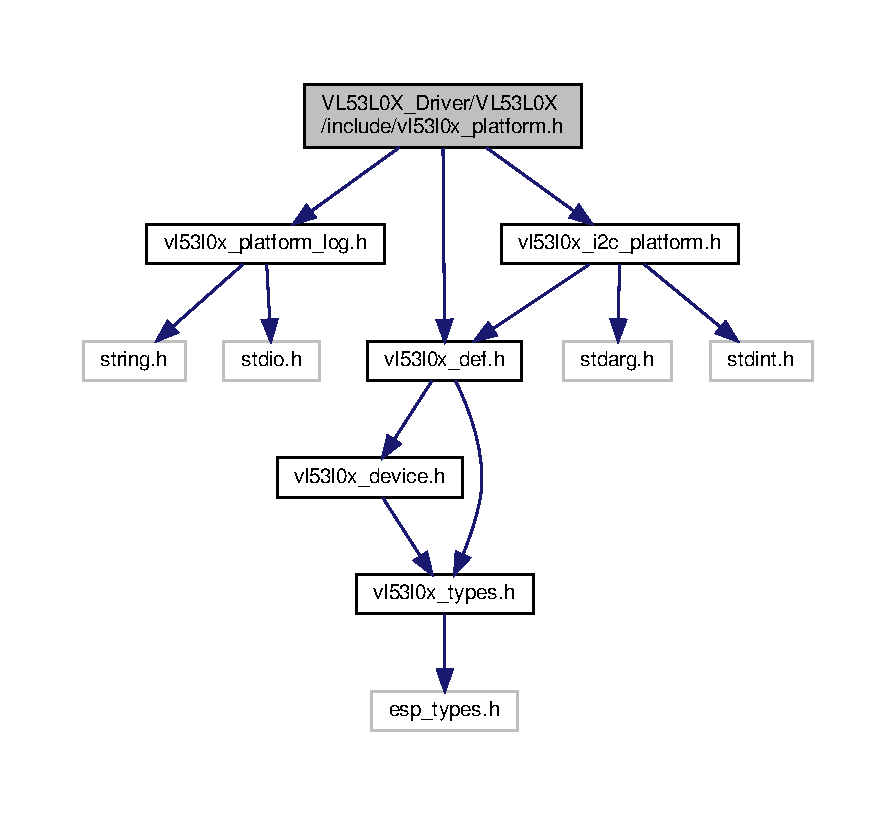
\includegraphics[width=350pt]{vl53l0x__platform_8h__incl}
\end{center}
\end{figure}
This graph shows which files directly or indirectly include this file\+:\nopagebreak
\begin{figure}[H]
\begin{center}
\leavevmode
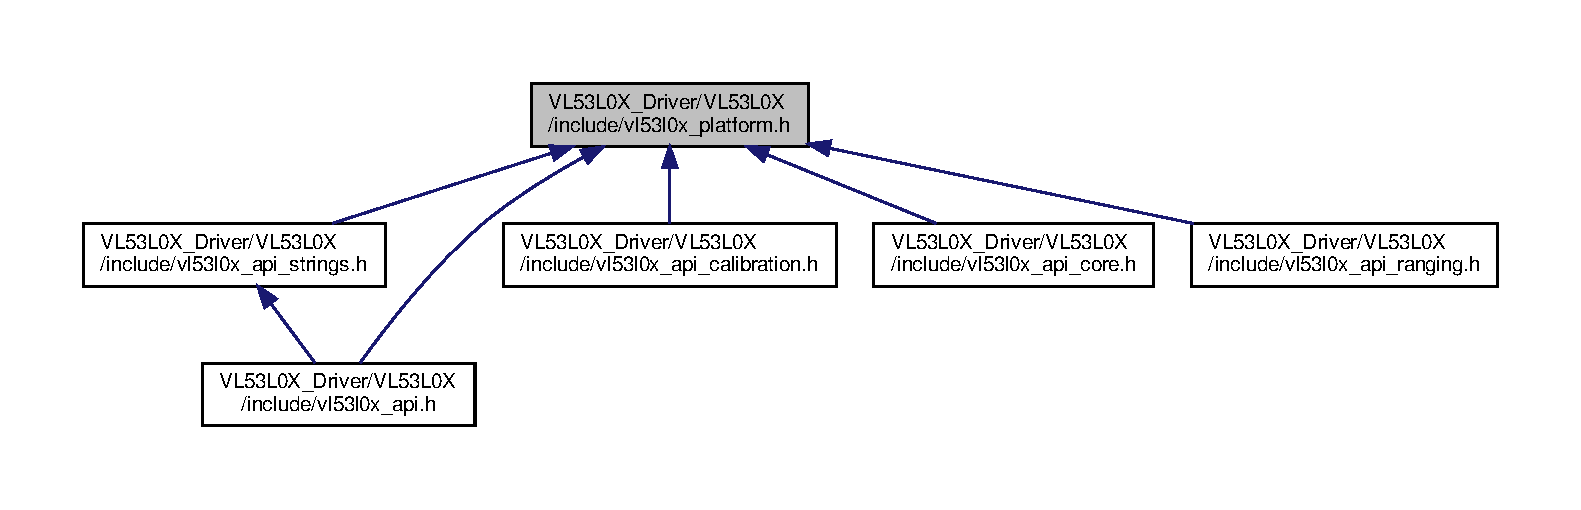
\includegraphics[width=350pt]{vl53l0x__platform_8h__dep__incl}
\end{center}
\end{figure}
\subsection*{Classes}
\begin{DoxyCompactItemize}
\item 
struct \hyperlink{structVL53L0X__Dev__t}{V\+L53\+L0\+X\+\_\+\+Dev\+\_\+t}
\begin{DoxyCompactList}\small\item\em Generic P\+AL device type that does link between A\+PI and platform abstraction layer. \end{DoxyCompactList}\end{DoxyCompactItemize}
\subsection*{Macros}
\begin{DoxyCompactItemize}
\item 
\mbox{\Hypertarget{vl53l0x__platform_8h_ae28444b326ec1d1af361df149506bd42}\label{vl53l0x__platform_8h_ae28444b326ec1d1af361df149506bd42}} 
\#define {\bfseries V\+L53\+\_\+\+M\+E\+A\+S\+U\+R\+E\+\_\+\+W\+A\+I\+T\+\_\+\+R\+E\+T\+R\+I\+ES}~10
\item 
\#define \hyperlink{group__VL53L0X__platform__group_ga21f3ef1fbe84f5cf77d989c95f21ad0a}{P\+A\+L\+Dev\+Data\+Get}(Dev,  field)~(Dev-\/$>$Data.\+field)
\begin{DoxyCompactList}\small\item\em Get ST private structure {\itshape \hyperlink{structVL53L0X__DevData__t}{V\+L53\+L0\+X\+\_\+\+Dev\+Data\+\_\+t}} data access. \end{DoxyCompactList}\item 
\#define \hyperlink{group__VL53L0X__platform__group_ga7d67a50d6fbce3ffdb71b4b3f7cbdf39}{P\+A\+L\+Dev\+Data\+Set}(Dev,  field,  data)~(Dev-\/$>$Data.\+field)=(data)
\begin{DoxyCompactList}\small\item\em Set ST private structure {\itshape \hyperlink{structVL53L0X__DevData__t}{V\+L53\+L0\+X\+\_\+\+Dev\+Data\+\_\+t}} data field. \end{DoxyCompactList}\end{DoxyCompactItemize}
\subsection*{Typedefs}
\begin{DoxyCompactItemize}
\item 
\mbox{\Hypertarget{vl53l0x__platform_8h_af085db7bd45480dfc98501d373fe8e4b}\label{vl53l0x__platform_8h_af085db7bd45480dfc98501d373fe8e4b}} 
typedef enum V\+L53\+L0\+X\+\_\+config {\bfseries V\+L53\+L0\+X\+\_\+config\+\_\+t}
\item 
typedef \hyperlink{structVL53L0X__Dev__t}{V\+L53\+L0\+X\+\_\+\+Dev\+\_\+t} $\ast$ \hyperlink{group__VL53L0X__platform__group_ga2d6405308b1dd524b462f1b8fb97d167}{V\+L53\+L0\+X\+\_\+\+D\+EV}
\begin{DoxyCompactList}\small\item\em Declare the device Handle as a pointer of the structure {\itshape \hyperlink{structVL53L0X__Dev__t}{V\+L53\+L0\+X\+\_\+\+Dev\+\_\+t}}. \end{DoxyCompactList}\end{DoxyCompactItemize}
\subsection*{Enumerations}
\begin{DoxyCompactItemize}
\item 
\mbox{\Hypertarget{vl53l0x__platform_8h_a1bb7e48805968e7aeea37520734a632d}\label{vl53l0x__platform_8h_a1bb7e48805968e7aeea37520734a632d}} 
enum {\bfseries V\+L53\+L0\+X\+\_\+config} \{ {\bfseries V\+L53\+L0\+X\+\_\+\+S\+E\+N\+S\+E\+\_\+\+D\+E\+F\+A\+U\+LT} = 0x00, 
{\bfseries V\+L53\+L0\+X\+\_\+\+S\+E\+N\+S\+E\+\_\+\+L\+O\+N\+G\+\_\+\+R\+A\+N\+GE} = 0x01, 
{\bfseries V\+L53\+L0\+X\+\_\+\+S\+E\+N\+S\+E\+\_\+\+H\+I\+G\+H\+\_\+\+S\+P\+E\+ED} = 0x02, 
{\bfseries V\+L53\+L0\+X\+\_\+\+S\+E\+N\+S\+E\+\_\+\+H\+I\+G\+H\+\_\+\+A\+C\+C\+U\+R\+A\+CY} = 0x03
 \}
\end{DoxyCompactItemize}
\subsection*{Functions}
\begin{DoxyCompactItemize}
\item 
V\+L53\+L0\+X\+\_\+\+Error \hyperlink{group__VL53L0X__registerAccess__group_gadec2e01eacfb71e35303673dba4c525a}{V\+L53\+L0\+X\+\_\+\+Lock\+Sequence\+Access} (\hyperlink{group__VL53L0X__platform__group_ga2d6405308b1dd524b462f1b8fb97d167}{V\+L53\+L0\+X\+\_\+\+D\+EV} Dev)
\item 
V\+L53\+L0\+X\+\_\+\+Error \hyperlink{group__VL53L0X__registerAccess__group_gaa842ffc920a56baf1e790b98f52c2973}{V\+L53\+L0\+X\+\_\+\+Unlock\+Sequence\+Access} (\hyperlink{group__VL53L0X__platform__group_ga2d6405308b1dd524b462f1b8fb97d167}{V\+L53\+L0\+X\+\_\+\+D\+EV} Dev)
\item 
V\+L53\+L0\+X\+\_\+\+Error \hyperlink{group__VL53L0X__registerAccess__group_ga1bd43902504d62efa30bb7d1334becb7}{V\+L53\+L0\+X\+\_\+\+Write\+Multi} (\hyperlink{group__VL53L0X__platform__group_ga2d6405308b1dd524b462f1b8fb97d167}{V\+L53\+L0\+X\+\_\+\+D\+EV} Dev, \hyperlink{vl53l0x__types_8h_aba7bc1797add20fe3efdf37ced1182c5}{uint8\+\_\+t} index, \hyperlink{vl53l0x__types_8h_aba7bc1797add20fe3efdf37ced1182c5}{uint8\+\_\+t} $\ast$pdata, \hyperlink{vl53l0x__types_8h_a435d1572bf3f880d55459d9805097f62}{uint32\+\_\+t} count)
\item 
V\+L53\+L0\+X\+\_\+\+Error \hyperlink{group__VL53L0X__registerAccess__group_ga7ada799fc93691cea5dde0cae5e3ab58}{V\+L53\+L0\+X\+\_\+\+Read\+Multi} (\hyperlink{group__VL53L0X__platform__group_ga2d6405308b1dd524b462f1b8fb97d167}{V\+L53\+L0\+X\+\_\+\+D\+EV} Dev, \hyperlink{vl53l0x__types_8h_aba7bc1797add20fe3efdf37ced1182c5}{uint8\+\_\+t} index, \hyperlink{vl53l0x__types_8h_aba7bc1797add20fe3efdf37ced1182c5}{uint8\+\_\+t} $\ast$pdata, \hyperlink{vl53l0x__types_8h_a435d1572bf3f880d55459d9805097f62}{uint32\+\_\+t} count)
\item 
V\+L53\+L0\+X\+\_\+\+Error \hyperlink{group__VL53L0X__registerAccess__group_ga17c6507a39dac954c01ef78a6bd27ca1}{V\+L53\+L0\+X\+\_\+\+Wr\+Byte} (\hyperlink{group__VL53L0X__platform__group_ga2d6405308b1dd524b462f1b8fb97d167}{V\+L53\+L0\+X\+\_\+\+D\+EV} Dev, \hyperlink{vl53l0x__types_8h_aba7bc1797add20fe3efdf37ced1182c5}{uint8\+\_\+t} index, \hyperlink{vl53l0x__types_8h_aba7bc1797add20fe3efdf37ced1182c5}{uint8\+\_\+t} data)
\item 
V\+L53\+L0\+X\+\_\+\+Error \hyperlink{group__VL53L0X__registerAccess__group_gadc1bb94017f349842e439db5a3d0fea8}{V\+L53\+L0\+X\+\_\+\+Wr\+Word} (\hyperlink{group__VL53L0X__platform__group_ga2d6405308b1dd524b462f1b8fb97d167}{V\+L53\+L0\+X\+\_\+\+D\+EV} Dev, \hyperlink{vl53l0x__types_8h_aba7bc1797add20fe3efdf37ced1182c5}{uint8\+\_\+t} index, \hyperlink{vl53l0x__types_8h_a273cf69d639a59973b6019625df33e30}{uint16\+\_\+t} data)
\item 
V\+L53\+L0\+X\+\_\+\+Error \hyperlink{group__VL53L0X__registerAccess__group_ga0a117141cf0e6b0a4b97935a367482d5}{V\+L53\+L0\+X\+\_\+\+Wr\+D\+Word} (\hyperlink{group__VL53L0X__platform__group_ga2d6405308b1dd524b462f1b8fb97d167}{V\+L53\+L0\+X\+\_\+\+D\+EV} Dev, \hyperlink{vl53l0x__types_8h_aba7bc1797add20fe3efdf37ced1182c5}{uint8\+\_\+t} index, \hyperlink{vl53l0x__types_8h_a435d1572bf3f880d55459d9805097f62}{uint32\+\_\+t} data)
\item 
V\+L53\+L0\+X\+\_\+\+Error \hyperlink{group__VL53L0X__registerAccess__group_gaab280eabdced8065bc4fb99e221e12f9}{V\+L53\+L0\+X\+\_\+\+Rd\+Byte} (\hyperlink{group__VL53L0X__platform__group_ga2d6405308b1dd524b462f1b8fb97d167}{V\+L53\+L0\+X\+\_\+\+D\+EV} Dev, \hyperlink{vl53l0x__types_8h_aba7bc1797add20fe3efdf37ced1182c5}{uint8\+\_\+t} index, \hyperlink{vl53l0x__types_8h_aba7bc1797add20fe3efdf37ced1182c5}{uint8\+\_\+t} $\ast$data)
\item 
V\+L53\+L0\+X\+\_\+\+Error \hyperlink{group__VL53L0X__registerAccess__group_gabff46b6c5c984c2b6b11783f1c640558}{V\+L53\+L0\+X\+\_\+\+Rd\+Word} (\hyperlink{group__VL53L0X__platform__group_ga2d6405308b1dd524b462f1b8fb97d167}{V\+L53\+L0\+X\+\_\+\+D\+EV} Dev, \hyperlink{vl53l0x__types_8h_aba7bc1797add20fe3efdf37ced1182c5}{uint8\+\_\+t} index, \hyperlink{vl53l0x__types_8h_a273cf69d639a59973b6019625df33e30}{uint16\+\_\+t} $\ast$data)
\item 
V\+L53\+L0\+X\+\_\+\+Error \hyperlink{group__VL53L0X__registerAccess__group_ga18d1e6fe40708046d611d581f20d735b}{V\+L53\+L0\+X\+\_\+\+Rd\+D\+Word} (\hyperlink{group__VL53L0X__platform__group_ga2d6405308b1dd524b462f1b8fb97d167}{V\+L53\+L0\+X\+\_\+\+D\+EV} Dev, \hyperlink{vl53l0x__types_8h_aba7bc1797add20fe3efdf37ced1182c5}{uint8\+\_\+t} index, \hyperlink{vl53l0x__types_8h_a435d1572bf3f880d55459d9805097f62}{uint32\+\_\+t} $\ast$data)
\item 
V\+L53\+L0\+X\+\_\+\+Error \hyperlink{group__VL53L0X__registerAccess__group_gaf8c163567d7906d16cad171957bf4198}{V\+L53\+L0\+X\+\_\+\+Update\+Byte} (\hyperlink{group__VL53L0X__platform__group_ga2d6405308b1dd524b462f1b8fb97d167}{V\+L53\+L0\+X\+\_\+\+D\+EV} Dev, \hyperlink{vl53l0x__types_8h_aba7bc1797add20fe3efdf37ced1182c5}{uint8\+\_\+t} index, \hyperlink{vl53l0x__types_8h_aba7bc1797add20fe3efdf37ced1182c5}{uint8\+\_\+t} And\+Data, \hyperlink{vl53l0x__types_8h_aba7bc1797add20fe3efdf37ced1182c5}{uint8\+\_\+t} Or\+Data)
\item 
V\+L53\+L0\+X\+\_\+\+Error \hyperlink{group__VL53L0X__platform__group_ga08518599bfc34a2c943dcd5fa14072de}{V\+L53\+L0\+X\+\_\+\+Polling\+Delay} (\hyperlink{group__VL53L0X__platform__group_ga2d6405308b1dd524b462f1b8fb97d167}{V\+L53\+L0\+X\+\_\+\+D\+EV} Dev)
\begin{DoxyCompactList}\small\item\em execute delay in all polling A\+PI call \end{DoxyCompactList}\end{DoxyCompactItemize}


\subsection{Detailed Description}
All end user O\+S/platform/application porting. 


\hypertarget{vl53l0x__platform__log_8h}{}\section{V\+L53\+L0\+X\+\_\+\+Driver/\+V\+L53\+L0\+X/include/vl53l0x\+\_\+platform\+\_\+log.h File Reference}
\label{vl53l0x__platform__log_8h}\index{V\+L53\+L0\+X\+\_\+\+Driver/\+V\+L53\+L0\+X/include/vl53l0x\+\_\+platform\+\_\+log.\+h@{V\+L53\+L0\+X\+\_\+\+Driver/\+V\+L53\+L0\+X/include/vl53l0x\+\_\+platform\+\_\+log.\+h}}


platform log function definition  


{\ttfamily \#include $<$stdio.\+h$>$}\newline
{\ttfamily \#include $<$string.\+h$>$}\newline
Include dependency graph for vl53l0x\+\_\+platform\+\_\+log.\+h\+:\nopagebreak
\begin{figure}[H]
\begin{center}
\leavevmode
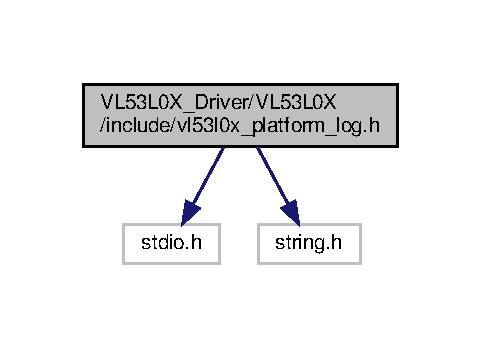
\includegraphics[width=231pt]{vl53l0x__platform__log_8h__incl}
\end{center}
\end{figure}
This graph shows which files directly or indirectly include this file\+:\nopagebreak
\begin{figure}[H]
\begin{center}
\leavevmode
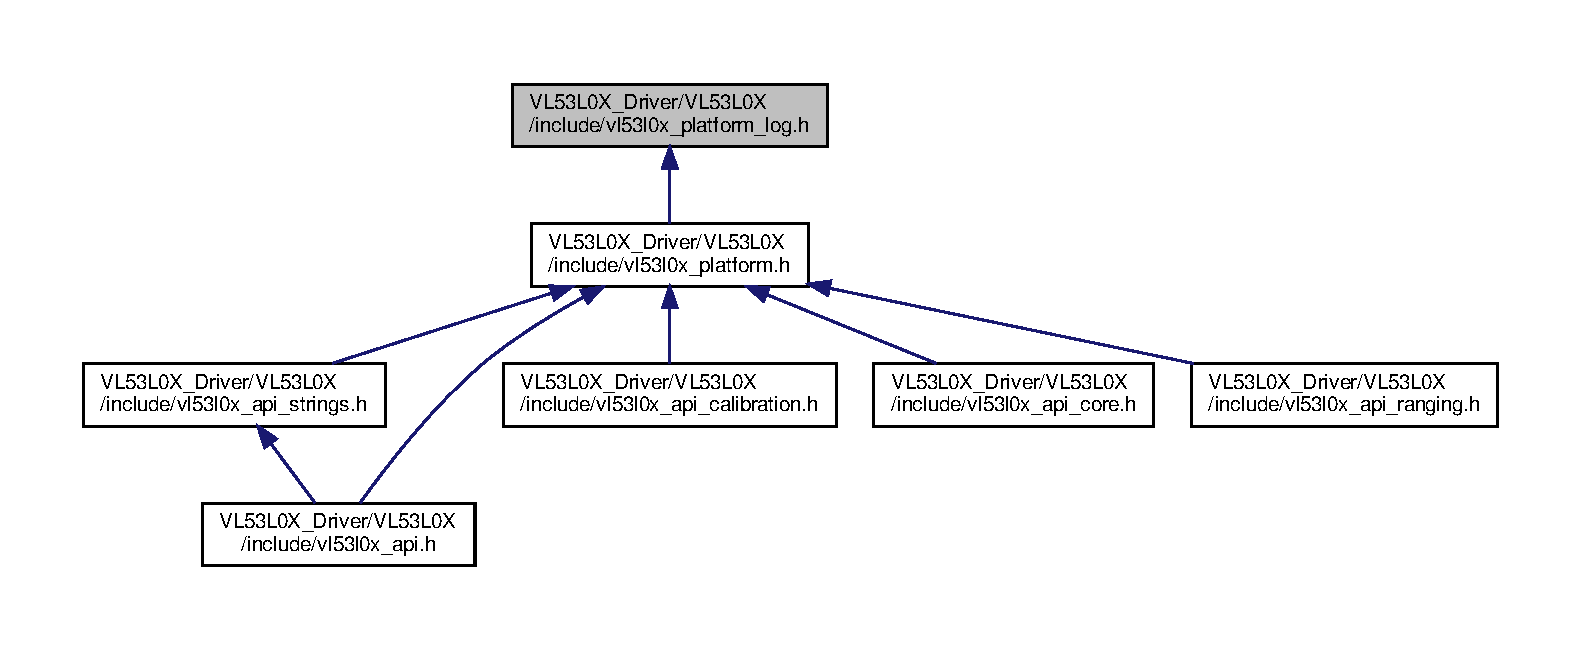
\includegraphics[width=350pt]{vl53l0x__platform__log_8h__dep__incl}
\end{center}
\end{figure}
\subsection*{Macros}
\begin{DoxyCompactItemize}
\item 
\mbox{\Hypertarget{vl53l0x__platform__log_8h_a39269d747b74f3e92edb6735fcae4cb6}\label{vl53l0x__platform__log_8h_a39269d747b74f3e92edb6735fcae4cb6}} 
\#define {\bfseries V\+L53\+L0\+X\+\_\+\+Err\+Log}(...)~(void)0
\item 
\mbox{\Hypertarget{vl53l0x__platform__log_8h_a04661915ba935d13648ff8b9bc5002cd}\label{vl53l0x__platform__log_8h_a04661915ba935d13648ff8b9bc5002cd}} 
\#define {\bfseries \+\_\+\+L\+O\+G\+\_\+\+F\+U\+N\+C\+T\+I\+O\+N\+\_\+\+S\+T\+A\+RT}(module,  fmt, ...)~(void)0
\item 
\mbox{\Hypertarget{vl53l0x__platform__log_8h_aa04b831714c5019aab1a35b6710462fb}\label{vl53l0x__platform__log_8h_aa04b831714c5019aab1a35b6710462fb}} 
\#define {\bfseries \+\_\+\+L\+O\+G\+\_\+\+F\+U\+N\+C\+T\+I\+O\+N\+\_\+\+E\+ND}(module,  status, ...)~(void)0
\item 
\mbox{\Hypertarget{vl53l0x__platform__log_8h_ac229b838e74d9a8ec587ddf1a7005e4a}\label{vl53l0x__platform__log_8h_ac229b838e74d9a8ec587ddf1a7005e4a}} 
\#define {\bfseries \+\_\+\+L\+O\+G\+\_\+\+F\+U\+N\+C\+T\+I\+O\+N\+\_\+\+E\+N\+D\+\_\+\+F\+MT}(module,  status,  fmt, ...)~(void)0
\item 
\mbox{\Hypertarget{vl53l0x__platform__log_8h_a8623ff32aa40f3ad27e1d4e374dd4bd3}\label{vl53l0x__platform__log_8h_a8623ff32aa40f3ad27e1d4e374dd4bd3}} 
\#define {\bfseries V\+L53\+L0\+X\+\_\+\+C\+O\+P\+Y\+S\+T\+R\+I\+NG}(str, ...)~strcpy(str, \#\#\+\_\+\+\_\+\+V\+A\+\_\+\+A\+R\+G\+S\+\_\+\+\_\+)
\end{DoxyCompactItemize}
\subsection*{Enumerations}
\begin{DoxyCompactItemize}
\item 
\mbox{\Hypertarget{vl53l0x__platform__log_8h_a09d9e56f5d4c14bc6d35272c7ee2692d}\label{vl53l0x__platform__log_8h_a09d9e56f5d4c14bc6d35272c7ee2692d}} 
enum \{ \newline
{\bfseries T\+R\+A\+C\+E\+\_\+\+L\+E\+V\+E\+L\+\_\+\+N\+O\+NE}, 
{\bfseries T\+R\+A\+C\+E\+\_\+\+L\+E\+V\+E\+L\+\_\+\+E\+R\+R\+O\+RS}, 
{\bfseries T\+R\+A\+C\+E\+\_\+\+L\+E\+V\+E\+L\+\_\+\+W\+A\+R\+N\+I\+NG}, 
{\bfseries T\+R\+A\+C\+E\+\_\+\+L\+E\+V\+E\+L\+\_\+\+I\+N\+FO}, 
\newline
{\bfseries T\+R\+A\+C\+E\+\_\+\+L\+E\+V\+E\+L\+\_\+\+D\+E\+B\+UG}, 
{\bfseries T\+R\+A\+C\+E\+\_\+\+L\+E\+V\+E\+L\+\_\+\+A\+LL}, 
{\bfseries T\+R\+A\+C\+E\+\_\+\+L\+E\+V\+E\+L\+\_\+\+I\+G\+N\+O\+RE}
 \}
\item 
\mbox{\Hypertarget{vl53l0x__platform__log_8h_ac8347fa324c6412b168db6df3464ad80}\label{vl53l0x__platform__log_8h_ac8347fa324c6412b168db6df3464ad80}} 
enum \{ {\bfseries T\+R\+A\+C\+E\+\_\+\+F\+U\+N\+C\+T\+I\+O\+N\+\_\+\+N\+O\+NE} = 0, 
{\bfseries T\+R\+A\+C\+E\+\_\+\+F\+U\+N\+C\+T\+I\+O\+N\+\_\+\+I2C} = 1, 
{\bfseries T\+R\+A\+C\+E\+\_\+\+F\+U\+N\+C\+T\+I\+O\+N\+\_\+\+A\+LL} = 0x7fffffff
 \}
\item 
\mbox{\Hypertarget{vl53l0x__platform__log_8h_abe821d0fac05333be298917dcb50ee1d}\label{vl53l0x__platform__log_8h_abe821d0fac05333be298917dcb50ee1d}} 
enum \{ {\bfseries T\+R\+A\+C\+E\+\_\+\+M\+O\+D\+U\+L\+E\+\_\+\+N\+O\+NE} = 0x0, 
{\bfseries T\+R\+A\+C\+E\+\_\+\+M\+O\+D\+U\+L\+E\+\_\+\+A\+PI} = 0x1, 
{\bfseries T\+R\+A\+C\+E\+\_\+\+M\+O\+D\+U\+L\+E\+\_\+\+P\+L\+A\+T\+F\+O\+RM} = 0x2, 
{\bfseries T\+R\+A\+C\+E\+\_\+\+M\+O\+D\+U\+L\+E\+\_\+\+A\+LL} = 0x7fffffff
 \}
\end{DoxyCompactItemize}


\subsection{Detailed Description}
platform log function definition 


\hypertarget{vl53l0x__types_8h}{}\section{V\+L53\+L0\+X\+\_\+\+Driver/\+V\+L53\+L0\+X/include/vl53l0x\+\_\+types.h File Reference}
\label{vl53l0x__types_8h}\index{V\+L53\+L0\+X\+\_\+\+Driver/\+V\+L53\+L0\+X/include/vl53l0x\+\_\+types.\+h@{V\+L53\+L0\+X\+\_\+\+Driver/\+V\+L53\+L0\+X/include/vl53l0x\+\_\+types.\+h}}


V\+L53\+L0X types definition.  


{\ttfamily \#include \char`\"{}esp\+\_\+types.\+h\char`\"{}}\newline
Include dependency graph for vl53l0x\+\_\+types.\+h\+:\nopagebreak
\begin{figure}[H]
\begin{center}
\leavevmode
\includegraphics[width=211pt]{vl53l0x__types_8h__incl}
\end{center}
\end{figure}
This graph shows which files directly or indirectly include this file\+:\nopagebreak
\begin{figure}[H]
\begin{center}
\leavevmode
\includegraphics[width=350pt]{vl53l0x__types_8h__dep__incl}
\end{center}
\end{figure}
\subsection*{Typedefs}
\begin{DoxyCompactItemize}
\item 
typedef \hyperlink{vl53l0x__types_8h_a435d1572bf3f880d55459d9805097f62}{uint32\+\_\+t} \hyperlink{vl53l0x__types_8h_afb910790161809fc76e1a274a6349384}{Fix\+Point1616\+\_\+t}
\end{DoxyCompactItemize}
\textbf{ }\par
\begin{DoxyCompactItemize}
\item 
\mbox{\Hypertarget{vl53l0x__types_8h_aaa5d1cd013383c889537491c3cfd9aad}\label{vl53l0x__types_8h_aaa5d1cd013383c889537491c3cfd9aad}} 
typedef unsigned long long {\bfseries uint64\+\_\+t}
\item 
\mbox{\Hypertarget{vl53l0x__types_8h_a435d1572bf3f880d55459d9805097f62}\label{vl53l0x__types_8h_a435d1572bf3f880d55459d9805097f62}} 
typedef unsigned int \hyperlink{vl53l0x__types_8h_a435d1572bf3f880d55459d9805097f62}{uint32\+\_\+t}
\begin{DoxyCompactList}\small\item\em Typedef defining 32 bit unsigned int type.~\newline
\hyperlink{structThe}{The} developer should modify this to suit the platform being deployed. \end{DoxyCompactList}\item 
\mbox{\Hypertarget{vl53l0x__types_8h_a32f2e37ee053cf2ce8ca28d1f74630e5}\label{vl53l0x__types_8h_a32f2e37ee053cf2ce8ca28d1f74630e5}} 
typedef int \hyperlink{vl53l0x__types_8h_a32f2e37ee053cf2ce8ca28d1f74630e5}{int32\+\_\+t}
\begin{DoxyCompactList}\small\item\em Typedef defining 32 bit int type.~\newline
\hyperlink{structThe}{The} developer should modify this to suit the platform being deployed. \end{DoxyCompactList}\item 
\mbox{\Hypertarget{vl53l0x__types_8h_a273cf69d639a59973b6019625df33e30}\label{vl53l0x__types_8h_a273cf69d639a59973b6019625df33e30}} 
typedef unsigned short \hyperlink{vl53l0x__types_8h_a273cf69d639a59973b6019625df33e30}{uint16\+\_\+t}
\begin{DoxyCompactList}\small\item\em Typedef defining 16 bit unsigned short type.~\newline
\hyperlink{structThe}{The} developer should modify this to suit the platform being deployed. \end{DoxyCompactList}\item 
\mbox{\Hypertarget{vl53l0x__types_8h_aa343fa3b3d06292b959ffdd4c4703b06}\label{vl53l0x__types_8h_aa343fa3b3d06292b959ffdd4c4703b06}} 
typedef short \hyperlink{vl53l0x__types_8h_aa343fa3b3d06292b959ffdd4c4703b06}{int16\+\_\+t}
\begin{DoxyCompactList}\small\item\em Typedef defining 16 bit short type.~\newline
\hyperlink{structThe}{The} developer should modify this to suit the platform being deployed. \end{DoxyCompactList}\item 
\mbox{\Hypertarget{vl53l0x__types_8h_aba7bc1797add20fe3efdf37ced1182c5}\label{vl53l0x__types_8h_aba7bc1797add20fe3efdf37ced1182c5}} 
typedef unsigned char \hyperlink{vl53l0x__types_8h_aba7bc1797add20fe3efdf37ced1182c5}{uint8\+\_\+t}
\begin{DoxyCompactList}\small\item\em Typedef defining 8 bit unsigned char type.~\newline
\hyperlink{structThe}{The} developer should modify this to suit the platform being deployed. \end{DoxyCompactList}\item 
\mbox{\Hypertarget{vl53l0x__types_8h_aef44329758059c91c76d334e8fc09700}\label{vl53l0x__types_8h_aef44329758059c91c76d334e8fc09700}} 
typedef signed char \hyperlink{vl53l0x__types_8h_aef44329758059c91c76d334e8fc09700}{int8\+\_\+t}
\begin{DoxyCompactList}\small\item\em Typedef defining 8 bit char type.~\newline
\hyperlink{structThe}{The} developer should modify this to suit the platform being deployed. \end{DoxyCompactList}\end{DoxyCompactItemize}



\subsection{Detailed Description}
V\+L53\+L0X types definition. 



\subsection{Typedef Documentation}
\mbox{\Hypertarget{vl53l0x__types_8h_afb910790161809fc76e1a274a6349384}\label{vl53l0x__types_8h_afb910790161809fc76e1a274a6349384}} 
\index{vl53l0x\+\_\+types.\+h@{vl53l0x\+\_\+types.\+h}!Fix\+Point1616\+\_\+t@{Fix\+Point1616\+\_\+t}}
\index{Fix\+Point1616\+\_\+t@{Fix\+Point1616\+\_\+t}!vl53l0x\+\_\+types.\+h@{vl53l0x\+\_\+types.\+h}}
\subsubsection{\texorpdfstring{Fix\+Point1616\+\_\+t}{FixPoint1616\_t}}
{\footnotesize\ttfamily typedef \hyperlink{vl53l0x__types_8h_a435d1572bf3f880d55459d9805097f62}{uint32\+\_\+t} \hyperlink{vl53l0x__types_8h_afb910790161809fc76e1a274a6349384}{Fix\+Point1616\+\_\+t}}

use where fractional values are expected

Given a floating point value f it\textquotesingle{}s .16 bit point is (int)(f$\ast$(1$<$$<$16)) 
%--- End generated contents ---

% Index
\backmatter
\newpage
\phantomsection
\clearemptydoublepage
\addcontentsline{toc}{chapter}{Index}
\printindex

\end{document}
